% Generated by Sphinx.
\def\sphinxdocclass{report}
\documentclass[a4paper,10pt,english]{sphinxmanual}
\usepackage[utf8]{inputenc}
\DeclareUnicodeCharacter{00A0}{\nobreakspace}
\usepackage{cmap}
\usepackage[T1]{fontenc}
\usepackage{amsfonts}
\usepackage{babel}
\usepackage{times}
\usepackage[Sonny]{fncychap}
\usepackage{longtable}
\usepackage{sphinx}
\usepackage{multirow}
\usepackage{eqparbox}


\addto\captionsenglish{\renewcommand{\figurename}{Fig. }}
\addto\captionsenglish{\renewcommand{\tablename}{Table }}
\SetupFloatingEnvironment{literal-block}{name=Listing }



\title{pgRouting Manual}
\date{May 31, 2018}
\release{v3.0.0-dev}
\author{pgRouting Contributors}
\newcommand{\sphinxlogo}{
\includegraphics{pgrouting.png}\par}
\renewcommand{\releasename}{Release}
\setcounter{tocdepth}{1}
\makeindex

\makeatletter
\def\PYG@reset{\let\PYG@it=\relax \let\PYG@bf=\relax%
    \let\PYG@ul=\relax \let\PYG@tc=\relax%
    \let\PYG@bc=\relax \let\PYG@ff=\relax}
\def\PYG@tok#1{\csname PYG@tok@#1\endcsname}
\def\PYG@toks#1+{\ifx\relax#1\empty\else%
    \PYG@tok{#1}\expandafter\PYG@toks\fi}
\def\PYG@do#1{\PYG@bc{\PYG@tc{\PYG@ul{%
    \PYG@it{\PYG@bf{\PYG@ff{#1}}}}}}}
\def\PYG#1#2{\PYG@reset\PYG@toks#1+\relax+\PYG@do{#2}}

\expandafter\def\csname PYG@tok@gd\endcsname{\def\PYG@tc##1{\textcolor[rgb]{0.63,0.00,0.00}{##1}}}
\expandafter\def\csname PYG@tok@gu\endcsname{\let\PYG@bf=\textbf\def\PYG@tc##1{\textcolor[rgb]{0.50,0.00,0.50}{##1}}}
\expandafter\def\csname PYG@tok@gt\endcsname{\def\PYG@tc##1{\textcolor[rgb]{0.00,0.27,0.87}{##1}}}
\expandafter\def\csname PYG@tok@gs\endcsname{\let\PYG@bf=\textbf}
\expandafter\def\csname PYG@tok@gr\endcsname{\def\PYG@tc##1{\textcolor[rgb]{1.00,0.00,0.00}{##1}}}
\expandafter\def\csname PYG@tok@cm\endcsname{\let\PYG@it=\textit\def\PYG@tc##1{\textcolor[rgb]{0.25,0.50,0.56}{##1}}}
\expandafter\def\csname PYG@tok@vg\endcsname{\def\PYG@tc##1{\textcolor[rgb]{0.73,0.38,0.84}{##1}}}
\expandafter\def\csname PYG@tok@vi\endcsname{\def\PYG@tc##1{\textcolor[rgb]{0.73,0.38,0.84}{##1}}}
\expandafter\def\csname PYG@tok@mh\endcsname{\def\PYG@tc##1{\textcolor[rgb]{0.13,0.50,0.31}{##1}}}
\expandafter\def\csname PYG@tok@cs\endcsname{\def\PYG@tc##1{\textcolor[rgb]{0.25,0.50,0.56}{##1}}\def\PYG@bc##1{\setlength{\fboxsep}{0pt}\colorbox[rgb]{1.00,0.94,0.94}{\strut ##1}}}
\expandafter\def\csname PYG@tok@ge\endcsname{\let\PYG@it=\textit}
\expandafter\def\csname PYG@tok@vc\endcsname{\def\PYG@tc##1{\textcolor[rgb]{0.73,0.38,0.84}{##1}}}
\expandafter\def\csname PYG@tok@il\endcsname{\def\PYG@tc##1{\textcolor[rgb]{0.13,0.50,0.31}{##1}}}
\expandafter\def\csname PYG@tok@go\endcsname{\def\PYG@tc##1{\textcolor[rgb]{0.20,0.20,0.20}{##1}}}
\expandafter\def\csname PYG@tok@cp\endcsname{\def\PYG@tc##1{\textcolor[rgb]{0.00,0.44,0.13}{##1}}}
\expandafter\def\csname PYG@tok@gi\endcsname{\def\PYG@tc##1{\textcolor[rgb]{0.00,0.63,0.00}{##1}}}
\expandafter\def\csname PYG@tok@gh\endcsname{\let\PYG@bf=\textbf\def\PYG@tc##1{\textcolor[rgb]{0.00,0.00,0.50}{##1}}}
\expandafter\def\csname PYG@tok@ni\endcsname{\let\PYG@bf=\textbf\def\PYG@tc##1{\textcolor[rgb]{0.84,0.33,0.22}{##1}}}
\expandafter\def\csname PYG@tok@nl\endcsname{\let\PYG@bf=\textbf\def\PYG@tc##1{\textcolor[rgb]{0.00,0.13,0.44}{##1}}}
\expandafter\def\csname PYG@tok@nn\endcsname{\let\PYG@bf=\textbf\def\PYG@tc##1{\textcolor[rgb]{0.05,0.52,0.71}{##1}}}
\expandafter\def\csname PYG@tok@no\endcsname{\def\PYG@tc##1{\textcolor[rgb]{0.38,0.68,0.84}{##1}}}
\expandafter\def\csname PYG@tok@na\endcsname{\def\PYG@tc##1{\textcolor[rgb]{0.25,0.44,0.63}{##1}}}
\expandafter\def\csname PYG@tok@nb\endcsname{\def\PYG@tc##1{\textcolor[rgb]{0.00,0.44,0.13}{##1}}}
\expandafter\def\csname PYG@tok@nc\endcsname{\let\PYG@bf=\textbf\def\PYG@tc##1{\textcolor[rgb]{0.05,0.52,0.71}{##1}}}
\expandafter\def\csname PYG@tok@nd\endcsname{\let\PYG@bf=\textbf\def\PYG@tc##1{\textcolor[rgb]{0.33,0.33,0.33}{##1}}}
\expandafter\def\csname PYG@tok@ne\endcsname{\def\PYG@tc##1{\textcolor[rgb]{0.00,0.44,0.13}{##1}}}
\expandafter\def\csname PYG@tok@nf\endcsname{\def\PYG@tc##1{\textcolor[rgb]{0.02,0.16,0.49}{##1}}}
\expandafter\def\csname PYG@tok@si\endcsname{\let\PYG@it=\textit\def\PYG@tc##1{\textcolor[rgb]{0.44,0.63,0.82}{##1}}}
\expandafter\def\csname PYG@tok@s2\endcsname{\def\PYG@tc##1{\textcolor[rgb]{0.25,0.44,0.63}{##1}}}
\expandafter\def\csname PYG@tok@nt\endcsname{\let\PYG@bf=\textbf\def\PYG@tc##1{\textcolor[rgb]{0.02,0.16,0.45}{##1}}}
\expandafter\def\csname PYG@tok@nv\endcsname{\def\PYG@tc##1{\textcolor[rgb]{0.73,0.38,0.84}{##1}}}
\expandafter\def\csname PYG@tok@s1\endcsname{\def\PYG@tc##1{\textcolor[rgb]{0.25,0.44,0.63}{##1}}}
\expandafter\def\csname PYG@tok@ch\endcsname{\let\PYG@it=\textit\def\PYG@tc##1{\textcolor[rgb]{0.25,0.50,0.56}{##1}}}
\expandafter\def\csname PYG@tok@m\endcsname{\def\PYG@tc##1{\textcolor[rgb]{0.13,0.50,0.31}{##1}}}
\expandafter\def\csname PYG@tok@gp\endcsname{\let\PYG@bf=\textbf\def\PYG@tc##1{\textcolor[rgb]{0.78,0.36,0.04}{##1}}}
\expandafter\def\csname PYG@tok@sh\endcsname{\def\PYG@tc##1{\textcolor[rgb]{0.25,0.44,0.63}{##1}}}
\expandafter\def\csname PYG@tok@ow\endcsname{\let\PYG@bf=\textbf\def\PYG@tc##1{\textcolor[rgb]{0.00,0.44,0.13}{##1}}}
\expandafter\def\csname PYG@tok@sx\endcsname{\def\PYG@tc##1{\textcolor[rgb]{0.78,0.36,0.04}{##1}}}
\expandafter\def\csname PYG@tok@bp\endcsname{\def\PYG@tc##1{\textcolor[rgb]{0.00,0.44,0.13}{##1}}}
\expandafter\def\csname PYG@tok@c1\endcsname{\let\PYG@it=\textit\def\PYG@tc##1{\textcolor[rgb]{0.25,0.50,0.56}{##1}}}
\expandafter\def\csname PYG@tok@o\endcsname{\def\PYG@tc##1{\textcolor[rgb]{0.40,0.40,0.40}{##1}}}
\expandafter\def\csname PYG@tok@kc\endcsname{\let\PYG@bf=\textbf\def\PYG@tc##1{\textcolor[rgb]{0.00,0.44,0.13}{##1}}}
\expandafter\def\csname PYG@tok@c\endcsname{\let\PYG@it=\textit\def\PYG@tc##1{\textcolor[rgb]{0.25,0.50,0.56}{##1}}}
\expandafter\def\csname PYG@tok@mf\endcsname{\def\PYG@tc##1{\textcolor[rgb]{0.13,0.50,0.31}{##1}}}
\expandafter\def\csname PYG@tok@err\endcsname{\def\PYG@bc##1{\setlength{\fboxsep}{0pt}\fcolorbox[rgb]{1.00,0.00,0.00}{1,1,1}{\strut ##1}}}
\expandafter\def\csname PYG@tok@mb\endcsname{\def\PYG@tc##1{\textcolor[rgb]{0.13,0.50,0.31}{##1}}}
\expandafter\def\csname PYG@tok@ss\endcsname{\def\PYG@tc##1{\textcolor[rgb]{0.32,0.47,0.09}{##1}}}
\expandafter\def\csname PYG@tok@sr\endcsname{\def\PYG@tc##1{\textcolor[rgb]{0.14,0.33,0.53}{##1}}}
\expandafter\def\csname PYG@tok@mo\endcsname{\def\PYG@tc##1{\textcolor[rgb]{0.13,0.50,0.31}{##1}}}
\expandafter\def\csname PYG@tok@kd\endcsname{\let\PYG@bf=\textbf\def\PYG@tc##1{\textcolor[rgb]{0.00,0.44,0.13}{##1}}}
\expandafter\def\csname PYG@tok@mi\endcsname{\def\PYG@tc##1{\textcolor[rgb]{0.13,0.50,0.31}{##1}}}
\expandafter\def\csname PYG@tok@kn\endcsname{\let\PYG@bf=\textbf\def\PYG@tc##1{\textcolor[rgb]{0.00,0.44,0.13}{##1}}}
\expandafter\def\csname PYG@tok@cpf\endcsname{\let\PYG@it=\textit\def\PYG@tc##1{\textcolor[rgb]{0.25,0.50,0.56}{##1}}}
\expandafter\def\csname PYG@tok@kr\endcsname{\let\PYG@bf=\textbf\def\PYG@tc##1{\textcolor[rgb]{0.00,0.44,0.13}{##1}}}
\expandafter\def\csname PYG@tok@s\endcsname{\def\PYG@tc##1{\textcolor[rgb]{0.25,0.44,0.63}{##1}}}
\expandafter\def\csname PYG@tok@kp\endcsname{\def\PYG@tc##1{\textcolor[rgb]{0.00,0.44,0.13}{##1}}}
\expandafter\def\csname PYG@tok@w\endcsname{\def\PYG@tc##1{\textcolor[rgb]{0.73,0.73,0.73}{##1}}}
\expandafter\def\csname PYG@tok@kt\endcsname{\def\PYG@tc##1{\textcolor[rgb]{0.56,0.13,0.00}{##1}}}
\expandafter\def\csname PYG@tok@sc\endcsname{\def\PYG@tc##1{\textcolor[rgb]{0.25,0.44,0.63}{##1}}}
\expandafter\def\csname PYG@tok@sb\endcsname{\def\PYG@tc##1{\textcolor[rgb]{0.25,0.44,0.63}{##1}}}
\expandafter\def\csname PYG@tok@k\endcsname{\let\PYG@bf=\textbf\def\PYG@tc##1{\textcolor[rgb]{0.00,0.44,0.13}{##1}}}
\expandafter\def\csname PYG@tok@se\endcsname{\let\PYG@bf=\textbf\def\PYG@tc##1{\textcolor[rgb]{0.25,0.44,0.63}{##1}}}
\expandafter\def\csname PYG@tok@sd\endcsname{\let\PYG@it=\textit\def\PYG@tc##1{\textcolor[rgb]{0.25,0.44,0.63}{##1}}}

\def\PYGZbs{\char`\\}
\def\PYGZus{\char`\_}
\def\PYGZob{\char`\{}
\def\PYGZcb{\char`\}}
\def\PYGZca{\char`\^}
\def\PYGZam{\char`\&}
\def\PYGZlt{\char`\<}
\def\PYGZgt{\char`\>}
\def\PYGZsh{\char`\#}
\def\PYGZpc{\char`\%}
\def\PYGZdl{\char`\$}
\def\PYGZhy{\char`\-}
\def\PYGZsq{\char`\'}
\def\PYGZdq{\char`\"}
\def\PYGZti{\char`\~}
% for compatibility with earlier versions
\def\PYGZat{@}
\def\PYGZlb{[}
\def\PYGZrb{]}
\makeatother

\renewcommand\PYGZsq{\textquotesingle}

\begin{document}

\maketitle
\tableofcontents
\phantomsection\label{index::doc}


pgRouting extends the \href{http://postgis.net}{PostGIS}\footnote[1]{
http://postgis.net
}/\href{http://postgresql.org}{PostgreSQL}\footnote[2]{
http://postgresql.org
} geospatial database to provide geospatial routing and other network analysis functionality.

This is the manual for pgRouting v3.0.0-dev.

{\includegraphics{{ccbysa}.png}\hspace*{\fill}}

The pgRouting Manual is licensed under a \href{http://creativecommons.org/licenses/by-sa/3.0/}{Creative Commons Attribution-Share Alike 3.0 License}\footnote[3]{
http://creativecommons.org/licenses/by-sa/3.0/
}. Feel free to use this material any way you like, but we ask that you attribute credit to the pgRouting Project and wherever possible, a link back to \href{http://pgrouting.org}{http://pgrouting.org}. For other licenses used in pgRouting see the {\hyperref[pgRouting\string-introduction:license]{\emph{Licensing}}} page.


\chapter{General}
\label{index:index}\label{index:table-of-contents}\label{index:general}

\section{Introduction}
\label{pgRouting-introduction:introduction}\label{pgRouting-introduction::doc}\label{pgRouting-introduction:id1}
pgRouting is an extension of \href{http://postgis.net}{PostGIS}\footnote[4]{
http://postgis.net
} and \href{http://postgresql.org}{PostgreSQL}\footnote[5]{
http://postgresql.org
} geospatial database and adds routing and other network analysis functionality. A predecessor of pgRouting – pgDijkstra, written by Sylvain Pasche from \href{http://camptocamp.com}{Camptocamp}\footnote[6]{
http://camptocamp.com
}, was later extended by \href{http://www.orkney.co.jp}{Orkney}\footnote[7]{
http://www.orkney.co.jp
} and renamed to pgRouting. The project is now supported and maintained by \href{http://georepublic.info}{Georepublic}\footnote[8]{
http://georepublic.info
}, \href{http://imaptools.com/}{iMaptools}\footnote[9]{
http://imaptools.com/
} and a broad user community.

pgRouting is part of \href{http://wiki.osgeo.org/wiki/OSGeo\_Community\_Projects}{OSGeo Community Projects}\footnote[10]{
http://wiki.osgeo.org/wiki/OSGeo\_Community\_Projects
} from the \href{http://osgeo.org}{OSGeo Foundation}\footnote[11]{
http://osgeo.org
} and included on \href{http://live.osgeo.org/}{OSGeo Live}\footnote[12]{
http://live.osgeo.org/
}.


\subsection{Licensing}
\label{pgRouting-introduction:licensing}\label{pgRouting-introduction:license}
The following licenses can be found in pgRouting:

\begin{tabular}{|p{0.475\linewidth}|p{0.475\linewidth}|}
\hline

\textbf{License}
 & \\
\hline
GNU General Public License, version 2
 & 
Most features of pgRouting are available under \href{http://www.gnu.org/licenses/gpl-2.0.html}{GNU General Public License, version 2}\protect\footnotemark[13].
\\
\hline
Boost Software License - Version 1.0
 & 
Some Boost extensions are available under \href{http://www.boost.org/LICENSE\_1\_0.txt}{Boost Software License - Version 1.0}\protect\footnotemark[14].
\\
\hline
MIT-X License
 & 
Some code contributed by iMaptools.com is available under MIT-X license.
\\
\hline
Creative Commons Attribution-Share Alike 3.0 License
 & 
The pgRouting Manual is licensed under a \href{http://creativecommons.org/licenses/by-sa/3.0/}{Creative Commons Attribution-Share Alike 3.0 License}\protect\footnotemark[15].
\\
\hline\end{tabular}

\footnotetext[13]{
http://www.gnu.org/licenses/gpl-2.0.html
}\footnotetext[14]{
http://www.boost.org/LICENSE\_1\_0.txt
}\footnotetext[15]{
http://creativecommons.org/licenses/by-sa/3.0/
}
In general license information should be included in the header of each source file.


\subsection{Contributors}
\label{pgRouting-introduction:contributors}

\subsubsection{This Release Contributors}
\label{pgRouting-introduction:this-release-contributors}

\paragraph{Individuals (in alphabetical order)}
\label{pgRouting-introduction:individuals-in-alphabetical-order}
Anthony Tasca, Virginia Vergara

And all the people that give us a little of their time making comments, finding issues, making pull requests etc.


\paragraph{Corporate Sponsors (in alphabetical order)}
\label{pgRouting-introduction:corporate-sponsors-in-alphabetical-order}
These are corporate entities that have contributed developer time, hosting, or direct monetary funding to the pgRouting project:
\begin{itemize}
\item {} 
\href{https://georepublic.info/en/}{Georepublic}\footnote[16]{
https://georepublic.info/en/
}

\item {} 
\href{https://developers.google.com/open-source/gsoc/}{Google Summer of Code}\footnote[17]{
https://developers.google.com/open-source/gsoc/
}

\item {} 
\href{http://imaptools.com}{iMaptools}\footnote[18]{
http://imaptools.com
}

\item {} 
\href{http://www.paragoncorporation.com/}{Paragon Corporation}\footnote[19]{
http://www.paragoncorporation.com/
}

\item {} 
\href{http://www.versaterm.com/}{Versaterm Inc.}\footnote[20]{
http://www.versaterm.com/
}

\end{itemize}


\subsubsection{Contributors Past \& Present:}
\label{pgRouting-introduction:contributors-past-present}

\paragraph{Individuals (in alphabetical order)}
\label{pgRouting-introduction:id2}
Akio Takubo, Andrea Nardelli, Anthony Tasca, Anton Patrushev, Ashraf Hossain, Christian Gonzalez, Daniel Kastl, Dave Potts, David Techer, Denis Rykov, Ema Miyawaki, Florian Thurkow, Frederic Junod, Gerald Fenoy, Jay Mahadeokar, Jinfu Leng, Kai Behncke, Kishore Kumar, Ko Nagase, Manikata Kondeti, Mario Basa, Martin Wiesenhaan,  Maxim Dubinin, Maoguang Wang, Mohamed Zia, Mukul Priya, Razequl Islam, Regina Obe, Rohith Reddy, Sarthak Agarwal, Stephen Woodbridge, Sylvain Housseman, Sylvain Pasche, Vidhan Jain, Virginia Vergara


\paragraph{Corporate Sponsors (in alphabetical order)}
\label{pgRouting-introduction:id3}
These are corporate entities that have contributed developer time, hosting, or direct monetary funding to the pgRouting project:
\begin{itemize}
\item {} 
Camptocamp

\item {} 
CSIS (University of Tokyo)

\item {} 
Georepublic

\item {} 
Google Summer of Code

\item {} 
iMaptools

\item {} 
Orkney

\item {} 
Paragon Corporation

\item {} 
Versaterm Inc.

\end{itemize}


\subsection{More Information}
\label{pgRouting-introduction:more-information}\begin{itemize}
\item {} 
The latest software, documentation and news items are available at the pgRouting web site \href{http://pgrouting.org}{http://pgrouting.org}.

\item {} 
PostgreSQL database server at the PostgreSQL main site \href{http://www.postgresql.org}{http://www.postgresql.org}.

\item {} 
PostGIS extension at the PostGIS project web site \href{http://postgis.net}{http://postgis.net}.

\item {} 
Boost C++ source libraries at \href{http://www.boost.org}{http://www.boost.org}.

\item {} 
Computational Geometry Algorithms Library (CGAL) at \href{http://www.cgal.org}{http://www.cgal.org}.

\item {} 
The Migration guide can be found at \href{https://github.com/pgRouting/pgrouting/wiki/Migration-Guide}{https://github.com/pgRouting/pgrouting/wiki/Migration-Guide}.

\end{itemize}


\section{Installation}
\label{pgRouting-installation:installation}\label{pgRouting-installation::doc}\label{pgRouting-installation:id1}\paragraph{Table of Contents}
\begin{itemize}
\item {} 
{\hyperref[pgRouting\string-installation:install\string-short]{\emph{Short Version}}}

\item {} 
{\hyperref[pgRouting\string-installation:install\string-get\string-sources]{\emph{Get the sources}}}

\item {} 
{\hyperref[pgRouting\string-installation:install\string-enable\string-db]{\emph{Enabling and upgrading in the database}}}

\item {} 
{\hyperref[pgRouting\string-installation:install\string-dependencies]{\emph{Dependencies}}}

\item {} 
{\hyperref[pgRouting\string-installation:install\string-configuring]{\emph{Configuring}}}

\item {} 
{\hyperref[pgRouting\string-installation:install\string-build]{\emph{Building}}}

\item {} 
{\hyperref[pgRouting\string-installation:install\string-testing]{\emph{Testing}}}

\end{itemize}

Instructions for downloading and installing binaries for different Operative systems instructions and additional notes and corrections not included in this documentation can be found in \href{https://github.com/pgRouting/pgrouting/wiki/Notes-on-Download\%2C-Installation-and-building-pgRouting}{Installation wiki}\footnote[21]{
https://github.com/pgRouting/pgrouting/wiki/Notes-on-Download\%2C-Installation-and-building-pgRouting
}

To use pgRouting postGIS needs to be installed, please read the information about installation in this \href{http://www.postgis.us/presentations/postgis\_install\_guide\_22.html}{Install Guide}\footnote[22]{
http://www.postgis.us/presentations/postgis\_install\_guide\_22.html
}


\subsection{Short Version}
\label{pgRouting-installation:short-version}\label{pgRouting-installation:install-short}
Extracting the tar ball

\begin{Verbatim}[commandchars=\\\{\}]
tar xvfz pgrouting\PYGZhy{}3.0.0.tar.gz
\PYG{n+nb}{cd} pgrouting\PYGZhy{}3.0.0
\end{Verbatim}

To compile assuming you have all the dependencies in your search path:

\begin{Verbatim}[commandchars=\\\{\}]
mkdir build
\PYG{n+nb}{cd} build
cmake  ..
make
sudo make install
\end{Verbatim}

Once pgRouting is installed, it needs to be enabled in each individual database you want to use it in.

\begin{Verbatim}[commandchars=\\\{\}]
createdb routing
psql routing \PYGZhy{}c \PYG{l+s+s1}{\PYGZsq{}CREATE EXTENSION postGIS\PYGZsq{}}
psql routing \PYGZhy{}c \PYG{l+s+s1}{\PYGZsq{}CREATE EXTENSION pgRouting\PYGZsq{}}
\end{Verbatim}


\subsection{Get the sources}
\label{pgRouting-installation:get-the-sources}\label{pgRouting-installation:install-get-sources}
The pgRouting latest release can be found in \href{https://github.com/pgRouting/pgrouting/releases/latest}{https://github.com/pgRouting/pgrouting/releases/latest}
\paragraph{wget}

To download this release:

\begin{Verbatim}[commandchars=\\\{\}]
wget \PYGZhy{}O pgrouting\PYGZhy{}3.0.0.tar.gz https://github.com/pgRouting/pgrouting/archive/v3.0.0.tar.gz
\end{Verbatim}

Goto {\hyperref[pgRouting\string-installation:install\string-short]{\emph{Short Version}}} to the extract and compile instructions.
\paragraph{git}

To download the repository

\begin{Verbatim}[commandchars=\\\{\}]
git clone git://github.com/pgRouting/pgrouting.git
\PYG{n+nb}{cd} pgrouting
git checkout v3.0.0
\end{Verbatim}

Goto {\hyperref[pgRouting\string-installation:install\string-short]{\emph{Short Version}}} to the compile instructions (there is no tar ball).


\subsection{Enabling and upgrading in the database}
\label{pgRouting-installation:install-enable-db}\label{pgRouting-installation:enabling-and-upgrading-in-the-database}\paragraph{Enabling the database}

pgRouting is an extension and depends on postGIS. Enabling postGIS before enabling pgRouting in the database

\begin{Verbatim}[commandchars=\\\{\}]
\PYG{k}{CREATE} \PYG{n}{EXTENSION} \PYG{n}{postgis}\PYG{p}{;}
\PYG{k}{CREATE} \PYG{n}{EXTENSION} \PYG{n}{pgrouting}\PYG{p}{;}
\end{Verbatim}
\paragraph{Upgrading the database}

To upgrade pgRouting in the database to version 3.0.0 use the following command:

\begin{Verbatim}[commandchars=\\\{\}]
\PYG{k}{ALTER} \PYG{n}{EXTENSION} \PYG{n}{pgrouting} \PYG{k}{UPDATE} \PYG{k}{TO} \PYG{l+s+ss}{\PYGZdq{}3.0.0\PYGZdq{}}\PYG{p}{;}
\end{Verbatim}

More information can be found in \href{https://www.postgresql.org/docs/current/static/sql-createextension.html}{https://www.postgresql.org/docs/current/static/sql-createextension.html}


\subsection{Dependencies}
\label{pgRouting-installation:install-dependencies}\label{pgRouting-installation:dependencies}\paragraph{Compilation Dependencies}

To be able to compile pgRouting, make sure that the following dependencies are met:
\begin{itemize}
\item {} 
C and C++0x compilers
* g++ version \textgreater{}= 4.8

\item {} 
Postgresql version \textgreater{}= 9.3

\item {} 
PostGIS version \textgreater{}= 2.2

\item {} 
The Boost Graph Library (BGL). Version \textgreater{}= 1.53

\item {} 
CMake \textgreater{}= 3.2

\item {} 
CGAL \textgreater{}=  4.2

\end{itemize}
\paragraph{optional dependencies}

For user's documentation
\begin{itemize}
\item {} 
Sphinx \textgreater{}= 1.1

\item {} 
Latex

\end{itemize}

For developer's documentation
\begin{itemize}
\item {} 
Doxygen \textgreater{}= 1.7

\end{itemize}

For testing
\begin{itemize}
\item {} 
pgtap

\item {} 
pg\_prove

\end{itemize}
\paragraph{Example: Installing dependencies on linux}

Installing the compilation dependencies
\paragraph{Database dependencies}

\begin{Verbatim}[commandchars=\\\{\}]
sudo apt\PYGZhy{}get install
    postgresql\PYGZhy{}10 \PYGZbs{}
    postgresql\PYGZhy{}server\PYGZhy{}dev\PYGZhy{}10 \PYGZbs{}
    postgresql\PYGZhy{}10\PYGZhy{}postgis
\end{Verbatim}
\paragraph{Build dependencies}

\begin{Verbatim}[commandchars=\\\{\}]
sudo apt\PYGZhy{}get install
    cmake \PYGZbs{}
    g++ \PYGZbs{}
    libboost\PYGZhy{}graph\PYGZhy{}dev \PYGZbs{}
    libcgal\PYGZhy{}dev
\end{Verbatim}
\paragraph{Optional dependencies}

For documentation and testing

\begin{Verbatim}[commandchars=\\\{\}]
sudo apt\PYGZhy{}get install \PYGZhy{}y python\PYGZhy{}sphinx \PYGZbs{}
    texlive \PYGZbs{}
    doxygen \PYGZbs{}
    libtap\PYGZhy{}parser\PYGZhy{}sourcehandler\PYGZhy{}pgtap\PYGZhy{}perl \PYGZbs{}
    postgresql\PYGZhy{}10\PYGZhy{}pgtap
\end{Verbatim}


\subsection{Configuring}
\label{pgRouting-installation:install-configuring}\label{pgRouting-installation:configuring}
pgRouting uses the \emph{cmake} system to do the configuration.

The build directory is different from the source directory

Create the build directory

\begin{Verbatim}[commandchars=\\\{\}]
\PYGZdl{} mkdir build
\end{Verbatim}


\subsubsection{Configurable variables}
\label{pgRouting-installation:configurable-variables}\paragraph{To see the variables that can be configured}

\begin{Verbatim}[commandchars=\\\{\}]
\PYGZdl{} \PYG{n+nb}{cd} build
\PYGZdl{} cmake \PYGZhy{}L ..
\end{Verbatim}
\paragraph{Configuring The Documentation}

Most of the effort of the documentation has being on the HTML files.
Some variables for the documentation:

\begin{tabulary}{\linewidth}{|L|L|L|}
\hline
\textsf{\relax 
Variable
} & \textsf{\relax 
Default
} & \textsf{\relax 
Comment
}\\
\hline
WITH\_DOC
 & 
BOOL=OFF
 & 
Turn on/off building the documentation
\\
\hline
BUILD\_HTML
 & 
BOOL=ON
 & 
If ON, turn on/off building HTML for user's documentation
\\
\hline
BUILD\_DOXY
 & 
BOOL=ON
 & 
If ON, turn on/off building HTML for developer's documentation
\\
\hline
BUILD\_LATEX
 & 
BOOL=OFF
 & 
If ON, turn on/off building PDF
\\
\hline
BUILD\_MAN
 & 
BOOL=OFF
 & 
If ON, turn on/off building MAN pages
\\
\hline
DOC\_USE\_BOOTSTRAP
 & 
BOOL=OFF
 & 
If ON, use sphinx-bootstrap for HTML pages of the users documentation
\\
\hline\end{tabulary}


Configuring with documentation

\begin{Verbatim}[commandchars=\\\{\}]
\PYGZdl{} cmake \PYGZhy{}DWITH\PYGZus{}DOC\PYG{o}{=}ON ..
\end{Verbatim}

\begin{notice}{note}{Note:}
Most of the effort of the documentation has being on the html files.
\end{notice}


\subsection{Building}
\label{pgRouting-installation:building}\label{pgRouting-installation:install-build}
Using \code{make} to build the code and the documentation

The following instructions start from \emph{path/to/pgrouting/build}

\begin{Verbatim}[commandchars=\\\{\}]
\PYGZdl{} make          \PYG{c+c1}{\PYGZsh{} build the code but not the documentation}
\PYGZdl{} make doc      \PYG{c+c1}{\PYGZsh{} build only the documentation}
\PYGZdl{} make all doc  \PYG{c+c1}{\PYGZsh{} build both the code and the documentation}
\end{Verbatim}

We have tested on several platforms, For installing or reinstalling all the steps are needed.

\begin{notice}{warning}{Warning:}
The sql signatures are configured and build in the \code{cmake} command.
\end{notice}
\paragraph{MinGW on Windows}

\begin{Verbatim}[commandchars=\\\{\}]
\PYGZdl{} mkdir build
\PYGZdl{} \PYG{n+nb}{cd} build
\PYGZdl{} cmake \PYGZhy{}G\PYG{l+s+s2}{\PYGZdq{}MSYS Makefiles\PYGZdq{}} ..
\PYGZdl{} make
\PYGZdl{} make install
\end{Verbatim}
\paragraph{Linux}

The following instructions start from \emph{path/to/pgrouting}

\begin{Verbatim}[commandchars=\\\{\}]
mkdir build
\PYG{n+nb}{cd} build
cmake  ..
make
sudo make install
\end{Verbatim}

When the configuration changes:

\begin{Verbatim}[commandchars=\\\{\}]
rm \PYGZhy{}rf build
\end{Verbatim}

and start the build process as mentioned above.


\subsection{Testing}
\label{pgRouting-installation:testing}\label{pgRouting-installation:install-testing}
Currently there is no \code{make test} and testing is done as follows

The following instructions start from \emph{path/to/pgrouting/}

\begin{Verbatim}[commandchars=\\\{\}]
tools/testers/algorithm\PYGZhy{}tester.pl
createdb  \PYGZhy{}U \PYGZlt{}user\PYGZgt{} \PYGZus{}\PYGZus{}\PYGZus{}pgr\PYGZus{}\PYGZus{}\PYGZus{}test\PYGZus{}\PYGZus{}\PYGZus{}
sh ./tools/testers/pg\PYGZus{}prove\PYGZus{}tests.sh \PYGZlt{}user\PYGZgt{}
dropdb  \PYGZhy{}U \PYGZlt{}user\PYGZgt{} \PYGZus{}\PYGZus{}\PYGZus{}pgr\PYGZus{}\PYGZus{}\PYGZus{}test\PYGZus{}\PYGZus{}\PYGZus{}
\end{Verbatim}


\subsection{See Also}
\label{pgRouting-installation:see-also}\paragraph{Indices and tables}
\begin{itemize}
\item {} 
\DUspan{xref,std,std-ref}{genindex}

\item {} 
\DUspan{xref,std,std-ref}{search}

\end{itemize}


\section{Support}
\label{support:support}\label{support::doc}\label{support:id1}
pgRouting community support is available through the \href{http://pgrouting.org/support.html}{pgRouting website}\footnote[23]{
http://pgrouting.org/support.html
}, \href{http://docs.pgrouting.org}{documentation}\footnote[24]{
http://docs.pgrouting.org
}, tutorials, mailing lists and others. If you’re looking for {\hyperref[support:support\string-commercial]{\emph{commercial support}}}, find below a list of companies providing pgRouting development and consulting services.


\subsection{Reporting Problems}
\label{support:reporting-problems}
Bugs are reported and managed in an \href{https://github.com/pgrouting/pgrouting/issues}{issue tracker}\footnote[25]{
https://github.com/pgrouting/pgrouting/issues
}. Please follow these steps:
\begin{enumerate}
\item {} 
Search the tickets to see if your problem has already been reported. If so, add any extra context you might have found, or at least indicate that you too are having the problem. This will help us prioritize common issues.

\item {} 
If your problem is unreported, create a \href{https://github.com/pgRouting/pgrouting/issues/new}{new issue}\footnote[26]{
https://github.com/pgRouting/pgrouting/issues/new
} for it.

\item {} 
In your report include explicit instructions to replicate your issue. The best tickets include the exact SQL necessary to replicate a problem.

\item {} 
If you can test older versions of PostGIS for your problem, please do. On your ticket, note the earliest version the problem appears.

\item {} 
For the versions where you can replicate the problem, note the operating system and version of pgRouting, PostGIS and PostgreSQL.

\item {} 
It is recommended to use the following wrapper on the problem to pin point the step that is causing the problem.

\end{enumerate}

\begin{Verbatim}[commandchars=\\\{\}]
\PYG{k}{SET} \PYG{n}{client\PYGZus{}min\PYGZus{}messages} \PYG{k}{TO} \PYG{n}{debug}\PYG{p}{;}
  \PYG{o}{\PYGZlt{}}\PYG{n}{your} \PYG{n}{code}\PYG{o}{\PYGZgt{}}
\PYG{k}{SET} \PYG{n}{client\PYGZus{}min\PYGZus{}messages} \PYG{k}{TO} \PYG{n}{notice}\PYG{p}{;}
\end{Verbatim}


\subsection{Mailing List and GIS StackExchange}
\label{support:mailing-list-and-gis-stackexchange}
There are two mailing lists for pgRouting hosted on OSGeo mailing list server:
\begin{itemize}
\item {} 
User mailing list: \href{http://lists.osgeo.org/mailman/listinfo/pgrouting-users}{http://lists.osgeo.org/mailman/listinfo/pgrouting-users}

\item {} 
Developer mailing list: \href{http://lists.osgeo.org/mailman/listinfo/pgrouting-dev}{http://lists.osgeo.org/mailman/listinfo/pgrouting-dev}

\end{itemize}

For general questions and topics about how to use pgRouting, please write to the user mailing list.

You can also ask at \href{http://gis.stackexchange.com/}{GIS StackExchange}\footnote[27]{
http://gis.stackexchange.com/
} and tag the question with \code{pgrouting}. Find all questions tagged with \code{pgrouting} under \href{http://gis.stackexchange.com/questions/tagged/pgrouting}{http://gis.stackexchange.com/questions/tagged/pgrouting} or subscribe to the \href{http://gis.stackexchange.com/feeds/tag?tagnames=pgrouting\&sort=newest}{pgRouting questions feed}\footnote[28]{
http://gis.stackexchange.com/feeds/tag?tagnames=pgrouting\&sort=newest
}.


\subsection{Commercial Support}
\label{support:support-commercial}\label{support:commercial-support}
For users who require professional support, development and consulting services, consider contacting any of the following organizations, which have significantly contributed to the development of pgRouting:

\begin{tabulary}{\linewidth}{|L|L|L|}
\hline

\textbf{Company}
 & 
\textbf{Offices in}
 & 
\textbf{Website}
\\
\hline
Georepublic
 & 
Germany, Japan
 & 
\href{https://georepublic.info}{https://georepublic.info}
\\
\hline
iMaptools
 & 
United States
 & 
\href{http://imaptools.com}{http://imaptools.com}
\\
\hline
Paragon Corporation
 & 
United States
 & 
\href{http://www.paragoncorporation.com}{http://www.paragoncorporation.com}
\\
\hline
Camptocamp
 & 
Switzerland, France
 & 
\href{http://www.camptocamp.com}{http://www.camptocamp.com}
\\
\hline\end{tabulary}

\begin{itemize}
\item {} 
{\hyperref[sampledata::doc]{\emph{\emph{Sample Data}}}} that is used in the examples of this manual.

\end{itemize}


\section{Sample Data}
\label{sampledata:sample-data}\label{sampledata::doc}
The documentation provides very simple example queries based on a small sample network.
To be able to execute the sample queries, run the following SQL commands to create a table with a small network data set.
\paragraph{Create table}

\begin{Verbatim}[commandchars=\\\{\}]
CREATE TABLE edge\PYGZus{}table (
    id BIGSERIAL,
    dir character varying,
    source BIGINT,
    target BIGINT,
    cost FLOAT,
    reverse\PYGZus{}cost FLOAT,
    capacity BIGINT,
    reverse\PYGZus{}capacity BIGINT,
    category\PYGZus{}id INTEGER,
    reverse\PYGZus{}category\PYGZus{}id INTEGER,
    x1 FLOAT,
    y1 FLOAT,
    x2 FLOAT,
    y2 FLOAT,
    the\PYGZus{}geom geometry
);
\end{Verbatim}
\paragraph{Insert data}

\begin{Verbatim}[commandchars=\\\{\}]
INSERT INTO edge\PYGZus{}table (
    category\PYGZus{}id, reverse\PYGZus{}category\PYGZus{}id,
    cost, reverse\PYGZus{}cost,
    capacity, reverse\PYGZus{}capacity,
    x1, y1,
    x2, y2) VALUES
(3, 1,    1,  1,  80, 130,   2,   0,    2, 1),
(3, 2,   \PYGZhy{}1,  1,  \PYGZhy{}1, 100,   2,   1,    3, 1),
(2, 1,   \PYGZhy{}1,  1,  \PYGZhy{}1, 130,   3,   1,    4, 1),
(2, 4,    1,  1, 100,  50,   2,   1,    2, 2),
(1, 4,    1, \PYGZhy{}1, 130,  \PYGZhy{}1,   3,   1,    3, 2),
(4, 2,    1,  1,  50, 100,   0,   2,    1, 2),
(4, 1,    1,  1,  50, 130,   1,   2,    2, 2),
(2, 1,    1,  1, 100, 130,   2,   2,    3, 2),
(1, 3,    1,  1, 130,  80,   3,   2,    4, 2),
(1, 4,    1,  1, 130,  50,   2,   2,    2, 3),
(1, 2,    1, \PYGZhy{}1, 130,  \PYGZhy{}1,   3,   2,    3, 3),
(2, 3,    1, \PYGZhy{}1, 100,  \PYGZhy{}1,   2,   3,    3, 3),
(2, 4,    1, \PYGZhy{}1, 100,  \PYGZhy{}1,   3,   3,    4, 3),
(3, 1,    1,  1,  80, 130,   2,   3,    2, 4),
(3, 4,    1,  1,  80,  50,   4,   2,    4, 3),
(3, 3,    1,  1,  80,  80,   4,   1,    4, 2),
(1, 2,    1,  1, 130, 100,   0.5, 3.5,  1.999999999999,3.5),
(4, 1,    1,  1,  50, 130,   3.5, 2.3,  3.5,4);

UPDATE edge\PYGZus{}table SET the\PYGZus{}geom = st\PYGZus{}makeline(st\PYGZus{}point(x1,y1),st\PYGZus{}point(x2,y2)),
dir = CASE WHEN (cost\PYGZgt{}0 AND reverse\PYGZus{}cost\PYGZgt{}0) THEN \PYGZsq{}B\PYGZsq{}   \PYGZhy{}\PYGZhy{} both ways
           WHEN (cost\PYGZgt{}0 AND reverse\PYGZus{}cost\PYGZlt{}0) THEN \PYGZsq{}FT\PYGZsq{}  \PYGZhy{}\PYGZhy{} direction of the LINESSTRING
           WHEN (cost\PYGZlt{}0 AND reverse\PYGZus{}cost\PYGZgt{}0) THEN \PYGZsq{}TF\PYGZsq{}  \PYGZhy{}\PYGZhy{} reverse direction of the LINESTRING
           ELSE \PYGZsq{}\PYGZsq{} END;                                \PYGZhy{}\PYGZhy{} unknown

\end{Verbatim}
\paragraph{Topology}
\begin{itemize}
\item {} 
Before you test a routing function use this query to create a topology (fills the \code{source} and \code{target} columns).

\end{itemize}

\begin{Verbatim}[commandchars=\\\{\}]
SELECT pgr\PYGZus{}createTopology(\PYGZsq{}edge\PYGZus{}table\PYGZsq{},0.001);

\end{Verbatim}
\paragraph{Points of interest}
\begin{itemize}
\item {} 
When points outside of the graph.

\item {} 
Used with the {\hyperref[withPoints\string-family:withpoints]{\emph{withPoints - Family of functions}}} functions.

\end{itemize}

\begin{Verbatim}[commandchars=\\\{\}]
CREATE TABLE pointsOfInterest(
    pid BIGSERIAL,
    x FLOAT,
    y FLOAT,
    edge\PYGZus{}id BIGINT,
    side CHAR,
    fraction FLOAT,
    the\PYGZus{}geom geometry,
    newPoint geometry
);

INSERT INTO pointsOfInterest (x, y, edge\PYGZus{}id, side, fraction) VALUES
(1.8, 0.4,   1, \PYGZsq{}l\PYGZsq{}, 0.4),
(4.2, 2.4,  15, \PYGZsq{}r\PYGZsq{}, 0.4),
(2.6, 3.2,  12, \PYGZsq{}l\PYGZsq{}, 0.6),
(0.3, 1.8,   6, \PYGZsq{}r\PYGZsq{}, 0.3),
(2.9, 1.8,   5, \PYGZsq{}l\PYGZsq{}, 0.8),
(2.2, 1.7,   4, \PYGZsq{}b\PYGZsq{}, 0.7);
UPDATE pointsOfInterest SET the\PYGZus{}geom = st\PYGZus{}makePoint(x,y);

UPDATE pointsOfInterest
    SET newPoint = ST\PYGZus{}LineInterpolatePoint(e.the\PYGZus{}geom, fraction)
    FROM edge\PYGZus{}table AS e WHERE edge\PYGZus{}id = id;

\end{Verbatim}
\paragraph{Restrictions}
\begin{itemize}
\item {} 
Used with the {\hyperref[pgr_trsp:trsp]{\emph{pgr\_trsp - Turn Restriction Shortest Path (TRSP)}}} functions.

\end{itemize}

\begin{Verbatim}[commandchars=\\\{\}]
CREATE TABLE restrictions (
    rid BIGINT NOT NULL,
    to\PYGZus{}cost FLOAT,
    target\PYGZus{}id BIGINT,
    from\PYGZus{}edge BIGINT,
    via\PYGZus{}path TEXT
);

INSERT INTO restrictions (rid, to\PYGZus{}cost, target\PYGZus{}id, from\PYGZus{}edge, via\PYGZus{}path) VALUES
(1, 100,  7,  4, NULL),
(1, 100, 11,  8, NULL),
(1, 100, 10,  7, NULL),
(2,   4,  8,  3, 5),
(3, 100,  9, 16, NULL);

\end{Verbatim}
\paragraph{Categories}
\begin{itemize}
\item {} 
Used with the {\hyperref[flow\string-family:maxflow]{\emph{Flow - Family of functions}}} functions.

\end{itemize}

\begin{Verbatim}[commandchars=\\\{\}]
/*
CREATE TABLE categories (
    category\PYGZus{}id INTEGER,
    category text,
    capacity BIGINT
);

INSERT INTO categories VALUES
(1, \PYGZsq{}Category 1\PYGZsq{}, 130),
(2, \PYGZsq{}Category 2\PYGZsq{}, 100),
(3, \PYGZsq{}Category 3\PYGZsq{},  80),
(4, \PYGZsq{}Category 4\PYGZsq{},  50);
*/
\end{Verbatim}
\paragraph{Vertex table}
\begin{itemize}
\item {} 
Used in some deprecated signatures or deprecated functions.

\end{itemize}

\begin{Verbatim}[commandchars=\\\{\}]

\PYGZhy{}\PYGZhy{} TODO check if this table is still used
CREATE TABLE vertex\PYGZus{}table (
    id SERIAL,
    x FLOAT,
    y FLOAT
);
INSERT INTO vertex\PYGZus{}table VALUES
(1,2,0), (2,2,1), (3,3,1), (4,4,1), (5,0,2), (6,1,2), (7,2,2),
(8,3,2), (9,4,2), (10,2,3), (11,3,3), (12,4,3), (13,2,4);

\end{Verbatim}


\subsection{Images}
\label{sampledata:images}\begin{itemize}
\item {} 
Red arrows correspond when \code{cost} \textgreater{} 0 in the edge table.

\item {} 
Blue arrows correspond when \code{reverse\_cost} \textgreater{} 0 in the edge table.

\item {} 
Points are outside the graph.

\item {} 
Click on the graph to enlarge.

\end{itemize}


\subsubsection{Network for queries marked as \texttt{directed} and \texttt{cost} and \texttt{reverse\_cost} columns are used}
\label{sampledata:network-for-queries-marked-as-directed-and-cost-and-reverse-cost-columns-are-used}\label{sampledata:fig1}
When working with city networks, this is recommended for point of view of vehicles.
\begin{figure}[htbp]
\centering
\capstart

\includegraphics{{Fig1-originalData}.png}
\caption{\textbf{Graph 1: Directed, with cost and reverse cost}}\end{figure}


\subsubsection{Network for queries marked as \texttt{undirected} and \texttt{cost} and \texttt{reverse\_cost} columns are used}
\label{sampledata:network-for-queries-marked-as-undirected-and-cost-and-reverse-cost-columns-are-used}\label{sampledata:fig2}
When working with city networks, this is recommended for point of view of pedestrians.
\begin{figure}[htbp]
\centering
\capstart

\scalebox{0.500000}{\includegraphics{{Fig6-undirected}.png}}
\caption{\textbf{Graph 2: Undirected, with cost and reverse cost}}\end{figure}


\subsubsection{Network for queries marked as \texttt{directed} and only \texttt{cost} column is used}
\label{sampledata:network-for-queries-marked-as-directed-and-only-cost-column-is-used}\label{sampledata:fig3}\begin{figure}[htbp]
\centering
\capstart

\scalebox{0.200000}{\includegraphics{{Fig2-cost}.png}}
\caption{\textbf{Graph 3: Directed, with cost}}\end{figure}


\subsubsection{Network for queries marked as \texttt{undirected} and only \texttt{cost} column is used}
\label{sampledata:fig4}\label{sampledata:network-for-queries-marked-as-undirected-and-only-cost-column-is-used}\begin{figure}[htbp]
\centering
\capstart

\scalebox{0.200000}{\includegraphics{{Fig4-costUndirected}.png}}
\caption{\textbf{Graph 4: Undirected, with cost}}\end{figure}


\subsubsection{Pick \& Deliver Data}
\label{sampledata:pickdeliverdata}\label{sampledata:pick-deliver-data}
\begin{Verbatim}[commandchars=\\\{\}]

DROP TABLE IF EXISTS customer CASCADE;
CREATE table customer (
    id BIGINT not null primary key,
    x DOUBLE PRECISION,
    y DOUBLE PRECISION,
    demand INTEGER,
    opentime INTEGER,
    closetime INTEGER,
    servicetime INTEGER,
    pindex BIGINT,
    dindex BIGINT
);


INSERT INTO customer(
  id,     x,    y, demand, opentime, closetime, servicetime, pindex, dindex) VALUES
(  0,    40,   50,     0,     0,  1236,    0,    0,    0),
(  1,    45,   68,   \PYGZhy{}10,   912,   967,   90,   11,    0),
(  2,    45,   70,   \PYGZhy{}20,   825,   870,   90,    6,    0),
(  3,    42,   66,    10,    65,   146,   90,    0,   75),
(  4,    42,   68,   \PYGZhy{}10,   727,   782,   90,    9,    0),
(  5,    42,   65,    10,    15,    67,   90,    0,    7),
(  6,    40,   69,    20,   621,   702,   90,    0,    2),
(  7,    40,   66,   \PYGZhy{}10,   170,   225,   90,    5,    0),
(  8,    38,   68,    20,   255,   324,   90,    0,   10),
(  9,    38,   70,    10,   534,   605,   90,    0,    4),
( 10,    35,   66,   \PYGZhy{}20,   357,   410,   90,    8,    0),
( 11,    35,   69,    10,   448,   505,   90,    0,    1),
( 12,    25,   85,   \PYGZhy{}20,   652,   721,   90,   18,    0),
( 13,    22,   75,    30,    30,    92,   90,    0,   17),
( 14,    22,   85,   \PYGZhy{}40,   567,   620,   90,   16,    0),
( 15,    20,   80,   \PYGZhy{}10,   384,   429,   90,   19,    0),
( 16,    20,   85,    40,   475,   528,   90,    0,   14),
( 17,    18,   75,   \PYGZhy{}30,    99,   148,   90,   13,    0),
( 18,    15,   75,    20,   179,   254,   90,    0,   12),
( 19,    15,   80,    10,   278,   345,   90,    0,   15),
( 20,    30,   50,    10,    10,    73,   90,    0,   24),
( 21,    30,   52,   \PYGZhy{}10,   914,   965,   90,   30,    0),
( 22,    28,   52,   \PYGZhy{}20,   812,   883,   90,   28,    0),
( 23,    28,   55,    10,   732,   777,    0,    0,  103),
( 24,    25,   50,   \PYGZhy{}10,    65,   144,   90,   20,    0),
( 25,    25,   52,    40,   169,   224,   90,    0,   27),
( 26,    25,   55,   \PYGZhy{}10,   622,   701,   90,   29,    0),
( 27,    23,   52,   \PYGZhy{}40,   261,   316,   90,   25,    0),
( 28,    23,   55,    20,   546,   593,   90,    0,   22),
( 29,    20,   50,    10,   358,   405,   90,    0,   26),
( 30,    20,   55,    10,   449,   504,   90,    0,   21),
( 31,    10,   35,   \PYGZhy{}30,   200,   237,   90,   32,    0),
( 32,    10,   40,    30,    31,   100,   90,    0,   31),
( 33,     8,   40,    40,    87,   158,   90,    0,   37),
( 34,     8,   45,   \PYGZhy{}30,   751,   816,   90,   38,    0),
( 35,     5,   35,    10,   283,   344,   90,    0,   39),
( 36,     5,   45,    10,   665,   716,    0,    0,  105),
( 37,     2,   40,   \PYGZhy{}40,   383,   434,   90,   33,    0),
( 38,     0,   40,    30,   479,   522,   90,    0,   34),
( 39,     0,   45,   \PYGZhy{}10,   567,   624,   90,   35,    0),
( 40,    35,   30,   \PYGZhy{}20,   264,   321,   90,   42,    0),
( 41,    35,   32,   \PYGZhy{}10,   166,   235,   90,   43,    0),
( 42,    33,   32,    20,    68,   149,   90,    0,   40),
( 43,    33,   35,    10,    16,    80,   90,    0,   41),
( 44,    32,   30,    10,   359,   412,   90,    0,   46),
( 45,    30,   30,    10,   541,   600,   90,    0,   48),
( 46,    30,   32,   \PYGZhy{}10,   448,   509,   90,   44,    0),
( 47,    30,   35,   \PYGZhy{}10,  1054,  1127,   90,   49,    0),
( 48,    28,   30,   \PYGZhy{}10,   632,   693,   90,   45,    0),
( 49,    28,   35,    10,  1001,  1066,   90,    0,   47),
( 50,    26,   32,    10,   815,   880,   90,    0,   52),
( 51,    25,   30,    10,   725,   786,    0,    0,  101),
( 52,    25,   35,   \PYGZhy{}10,   912,   969,   90,   50,    0),
( 53,    44,    5,    20,   286,   347,   90,    0,   58),
( 54,    42,   10,    40,   186,   257,   90,    0,   60),
( 55,    42,   15,   \PYGZhy{}40,    95,   158,   90,   57,    0),
( 56,    40,    5,    30,   385,   436,   90,    0,   59),
( 57,    40,   15,    40,    35,    87,   90,    0,   55),
( 58,    38,    5,   \PYGZhy{}20,   471,   534,   90,   53,    0),
( 59,    38,   15,   \PYGZhy{}30,   651,   740,   90,   56,    0),
( 60,    35,    5,   \PYGZhy{}40,   562,   629,   90,   54,    0),
( 61,    50,   30,   \PYGZhy{}10,   531,   610,   90,   67,    0),
( 62,    50,   35,    20,   262,   317,   90,    0,   68),
( 63,    50,   40,    50,   171,   218,   90,    0,   74),
( 64,    48,   30,    10,   632,   693,    0,    0,  102),
( 65,    48,   40,    10,    76,   129,   90,    0,   72),
( 66,    47,   35,    10,   826,   875,   90,    0,   69),
( 67,    47,   40,    10,    12,    77,   90,    0,   61),
( 68,    45,   30,   \PYGZhy{}20,   734,   777,   90,   62,    0),
( 69,    45,   35,   \PYGZhy{}10,   916,   969,   90,   66,    0),
( 70,    95,   30,   \PYGZhy{}30,   387,   456,   90,   81,    0),
( 71,    95,   35,    20,   293,   360,   90,    0,   77),
( 72,    53,   30,   \PYGZhy{}10,   450,   505,   90,   65,    0),
( 73,    92,   30,   \PYGZhy{}10,   478,   551,   90,   76,    0),
( 74,    53,   35,   \PYGZhy{}50,   353,   412,   90,   63,    0),
( 75,    45,   65,   \PYGZhy{}10,   997,  1068,   90,    3,    0),
( 76,    90,   35,    10,   203,   260,   90,    0,   73),
( 77,    88,   30,   \PYGZhy{}20,   574,   643,   90,   71,    0),
( 78,    88,   35,    20,   109,   170,    0,    0,  104),
( 79,    87,   30,    10,   668,   731,   90,    0,   80),
( 80,    85,   25,   \PYGZhy{}10,   769,   820,   90,   79,    0),
( 81,    85,   35,    30,    47,   124,   90,    0,   70),
( 82,    75,   55,    20,   369,   420,   90,    0,   85),
( 83,    72,   55,   \PYGZhy{}20,   265,   338,   90,   87,    0),
( 84,    70,   58,    20,   458,   523,   90,    0,   89),
( 85,    68,   60,   \PYGZhy{}20,   555,   612,   90,   82,    0),
( 86,    66,   55,    10,   173,   238,   90,    0,   91),
( 87,    65,   55,    20,    85,   144,   90,    0,   83),
( 88,    65,   60,   \PYGZhy{}10,   645,   708,   90,   90,    0),
( 89,    63,   58,   \PYGZhy{}20,   737,   802,   90,   84,    0),
( 90,    60,   55,    10,    20,    84,   90,    0,   88),
( 91,    60,   60,   \PYGZhy{}10,   836,   889,   90,   86,    0),
( 92,    67,   85,    20,   368,   441,   90,    0,   93),
( 93,    65,   85,   \PYGZhy{}20,   475,   518,   90,   92,    0),
( 94,    65,   82,   \PYGZhy{}10,   285,   336,   90,   96,    0),
( 95,    62,   80,   \PYGZhy{}20,   196,   239,   90,   98,    0),
( 96,    60,   80,    10,    95,   156,   90,    0,   94),
( 97,    60,   85,    30,   561,   622,    0,    0,  106),
( 98,    58,   75,    20,    30,    84,   90,    0,   95),
( 99,    55,   80,   \PYGZhy{}20,   743,   820,   90,  100,    0),
( 100,   55,   85,    20,   647,   726,   90,    0,   99),
( 101,   25,   30,   \PYGZhy{}10,   725,   786,   90,   51,    0),
( 102,   48,   30,   \PYGZhy{}10,   632,   693,   90,   64,    0),
( 103,   28,   55,   \PYGZhy{}10,   732,   777,   90,   23,    0),
( 104,   88,   35,   \PYGZhy{}20,   109,   170,   90,   78,    0),
( 105,    5,   45,   \PYGZhy{}10,   665,   716,   90,   36,    0),
( 106,   60,   85,   \PYGZhy{}30,   561,   622,   90,   97,    0);
\end{Verbatim}


\chapter{Pgrouting Concepts}
\label{index:pgrouting-concepts}

\section{pgRouting Concepts}
\label{pgRouting-concepts:pgrouting-concepts}\label{pgRouting-concepts::doc}\label{pgRouting-concepts:id1}\setbox0\vbox{
\begin{minipage}{0.95\linewidth}
\textbf{Contents}

\medskip

\begin{itemize}
\item {} 
\phantomsection\label{pgRouting-concepts:id13}{\hyperref[pgRouting\string-concepts:pgrouting\string-concepts]{\emph{pgRouting Concepts}}}
\begin{itemize}
\item {} 
\phantomsection\label{pgRouting-concepts:id14}{\hyperref[pgRouting\string-concepts:getting\string-started]{\emph{Getting Started}}}
\begin{itemize}
\item {} 
\phantomsection\label{pgRouting-concepts:id15}{\hyperref[pgRouting\string-concepts:create\string-a\string-routing\string-database]{\emph{Create a routing Database}}}

\item {} 
\phantomsection\label{pgRouting-concepts:id16}{\hyperref[pgRouting\string-concepts:load\string-data]{\emph{Load Data}}}

\item {} 
\phantomsection\label{pgRouting-concepts:id17}{\hyperref[pgRouting\string-concepts:build\string-a\string-routing\string-topology]{\emph{Build a Routing Topology}}}

\item {} 
\phantomsection\label{pgRouting-concepts:id18}{\hyperref[pgRouting\string-concepts:check\string-the\string-routing\string-topology]{\emph{Check the Routing Topology}}}

\item {} 
\phantomsection\label{pgRouting-concepts:id19}{\hyperref[pgRouting\string-concepts:compute\string-a\string-path]{\emph{Compute a Path}}}

\end{itemize}

\item {} 
\phantomsection\label{pgRouting-concepts:id20}{\hyperref[pgRouting\string-concepts:inner\string-queries]{\emph{Inner Queries}}}
\begin{itemize}
\item {} 
\phantomsection\label{pgRouting-concepts:id21}{\hyperref[pgRouting\string-concepts:description\string-of\string-the\string-edges\string-sql\string-query\string-for\string-dijkstra\string-like\string-functions]{\emph{Description of the edges\_sql query for dijkstra like functions}}}

\item {} 
\phantomsection\label{pgRouting-concepts:id22}{\hyperref[pgRouting\string-concepts:description\string-of\string-the\string-edges\string-sql\string-query\string-id\string-is\string-not\string-necessary]{\emph{Description of the edges\_sql query (id is not necessary)}}}

\item {} 
\phantomsection\label{pgRouting-concepts:id23}{\hyperref[pgRouting\string-concepts:description\string-of\string-the\string-parameters\string-of\string-the\string-signatures]{\emph{Description of the parameters of the signatures}}}

\item {} 
\phantomsection\label{pgRouting-concepts:id24}{\hyperref[pgRouting\string-concepts:description\string-of\string-the\string-edges\string-sql\string-query\string-for\string-astar\string-like\string-functions]{\emph{Description of the edges\_sql query for astar like functions}}}

\item {} 
\phantomsection\label{pgRouting-concepts:id25}{\hyperref[pgRouting\string-concepts:description\string-of\string-the\string-edges\string-sql\string-query\string-for\string-max\string-flow\string-like\string-functions]{\emph{Description of the edges\_sql query for Max-flow like functions}}}

\item {} 
\phantomsection\label{pgRouting-concepts:id26}{\hyperref[pgRouting\string-concepts:description\string-of\string-the\string-points\string-sql\string-query]{\emph{Description of the Points SQL query}}}

\end{itemize}

\item {} 
\phantomsection\label{pgRouting-concepts:id27}{\hyperref[pgRouting\string-concepts:return\string-columns\string-values]{\emph{Return columns \& values}}}
\begin{itemize}
\item {} 
\phantomsection\label{pgRouting-concepts:id28}{\hyperref[pgRouting\string-concepts:description\string-of\string-the\string-return\string-values\string-for\string-a\string-path]{\emph{Description of the return values for a path}}}

\item {} 
\phantomsection\label{pgRouting-concepts:id29}{\hyperref[pgRouting\string-concepts:description\string-of\string-the\string-return\string-values\string-for\string-a\string-cost\string-function]{\emph{Description of the return values for a Cost function}}}

\item {} 
\phantomsection\label{pgRouting-concepts:id30}{\hyperref[pgRouting\string-concepts:description\string-of\string-the\string-return\string-values]{\emph{Description of the Return Values}}}

\end{itemize}

\item {} 
\phantomsection\label{pgRouting-concepts:id31}{\hyperref[pgRouting\string-concepts:advanced\string-topics]{\emph{Advanced Topics}}}
\begin{itemize}
\item {} 
\phantomsection\label{pgRouting-concepts:id32}{\hyperref[pgRouting\string-concepts:routing\string-topology]{\emph{Routing Topology}}}

\item {} 
\phantomsection\label{pgRouting-concepts:id33}{\hyperref[pgRouting\string-concepts:graph\string-analytics]{\emph{Graph Analytics}}}

\item {} 
\phantomsection\label{pgRouting-concepts:id34}{\hyperref[pgRouting\string-concepts:analyze\string-a\string-graph]{\emph{Analyze a Graph}}}

\item {} 
\phantomsection\label{pgRouting-concepts:id35}{\hyperref[pgRouting\string-concepts:analyze\string-one\string-way\string-streets]{\emph{Analyze One Way Streets}}}
\begin{itemize}
\item {} 
\phantomsection\label{pgRouting-concepts:id36}{\hyperref[pgRouting\string-concepts:example]{\emph{Example}}}

\end{itemize}

\end{itemize}

\item {} 
\phantomsection\label{pgRouting-concepts:id37}{\hyperref[pgRouting\string-concepts:performance\string-tips]{\emph{Performance Tips}}}
\begin{itemize}
\item {} 
\phantomsection\label{pgRouting-concepts:id38}{\hyperref[pgRouting\string-concepts:for\string-the\string-routing\string-functions]{\emph{For the Routing functions}}}

\item {} 
\phantomsection\label{pgRouting-concepts:id39}{\hyperref[pgRouting\string-concepts:for\string-the\string-topology\string-functions]{\emph{For the topology functions:}}}

\end{itemize}

\item {} 
\phantomsection\label{pgRouting-concepts:id40}{\hyperref[pgRouting\string-concepts:how\string-to\string-contribute]{\emph{How to contribute}}}

\end{itemize}

\end{itemize}
\end{minipage}}
\begin{center}\setlength{\fboxsep}{5pt}\shadowbox{\box0}\end{center}


\subsection{Getting Started}
\label{pgRouting-concepts:getting-started}\label{pgRouting-concepts:id2}
This is a simple guide to walk you through the steps of getting started
with pgRouting. In this guide we will cover:
\setbox0\vbox{
\begin{minipage}{0.95\linewidth}
\begin{itemize}
\item {} 
\phantomsection\label{pgRouting-concepts:id41}{\hyperref[pgRouting\string-concepts:create\string-a\string-routing\string-database]{\emph{Create a routing Database}}}

\item {} 
\phantomsection\label{pgRouting-concepts:id42}{\hyperref[pgRouting\string-concepts:load\string-data]{\emph{Load Data}}}

\item {} 
\phantomsection\label{pgRouting-concepts:id43}{\hyperref[pgRouting\string-concepts:build\string-a\string-routing\string-topology]{\emph{Build a Routing Topology}}}

\item {} 
\phantomsection\label{pgRouting-concepts:id44}{\hyperref[pgRouting\string-concepts:check\string-the\string-routing\string-topology]{\emph{Check the Routing Topology}}}

\item {} 
\phantomsection\label{pgRouting-concepts:id45}{\hyperref[pgRouting\string-concepts:compute\string-a\string-path]{\emph{Compute a Path}}}

\end{itemize}
\end{minipage}}
\begin{center}\setlength{\fboxsep}{5pt}\shadowbox{\box0}\end{center}


\subsubsection{Create a routing Database}
\label{pgRouting-concepts:create-database}\label{pgRouting-concepts:create-a-routing-database}
The first thing we need to do is create a database and load pgrouting in
the database. Typically you will create a database for each project. Once
you have a database to work in, your can load your data and build your
application in that database. This makes it easy to move your project
later if you want to to say a production server.

For Postgresql 9.2 and later versions

\begin{Verbatim}[commandchars=\\\{\}]
createdb mydatabase
psql mydatabase \PYGZhy{}c \PYG{l+s+s2}{\PYGZdq{}create extension postgis\PYGZdq{}}
psql mydatabase \PYGZhy{}c \PYG{l+s+s2}{\PYGZdq{}create extension pgrouting\PYGZdq{}}
\end{Verbatim}


\subsubsection{Load Data}
\label{pgRouting-concepts:load-data}\label{pgRouting-concepts:id4}
How you load your data will depend in what form it comes it. There are
various OpenSource tools that can help you, like:
\begin{quote}\begin{description}
\item[{osm2pgrouting}] \leavevmode\begin{itemize}
\item {} 
this is a tool for loading OSM data into postgresql with pgRouting requirements

\end{itemize}

\item[{shp2pgsql}] \leavevmode\begin{itemize}
\item {} 
this is the postgresql shapefile loader

\end{itemize}

\item[{ogr2ogr}] \leavevmode\begin{itemize}
\item {} 
this is a vector data conversion utility

\end{itemize}

\item[{osm2pgsql}] \leavevmode\begin{itemize}
\item {} 
this is a tool for loading OSM data into postgresql

\end{itemize}

\end{description}\end{quote}

So these tools and probably others will allow you to read vector data so that
you may then load that data into your database as a table of some kind. At this
point you need to know a little about your data structure and content. One easy
way to browse your new data table is with pgAdmin3 or phpPgAdmin.


\subsubsection{Build a Routing Topology}
\label{pgRouting-concepts:build-a-routing-topology}\label{pgRouting-concepts:build-topology}
Next we need to build a topology for our street data. What this means is that
for any given edge in your street data the ends of that edge will be connected
to a unique node and to other edges that are also connected to that same unique
node. Once all the edges are connected to nodes we have a graph that can be
used for routing with pgrouting. We provide a tool that will help with this:

\begin{notice}{note}{Note:}
this step is not needed if data is loaded with \emph{osm2pgrouting}
\end{notice}

\begin{Verbatim}[commandchars=\\\{\}]
\PYG{k}{select} \PYG{n}{pgr\PYGZus{}createTopology}\PYG{p}{(}\PYG{l+s+s1}{\PYGZsq{}myroads\PYGZsq{}}\PYG{p}{,} \PYG{l+m+mi}{0}\PYG{p}{.}\PYG{l+m+mi}{000001}\PYG{p}{)}\PYG{p}{;}
\end{Verbatim}
\begin{itemize}
\item {} 
{\hyperref[pgr_createTopology:pgr\string-create\string-topology]{\emph{pgr\_createTopology}}}

\end{itemize}


\subsubsection{Check the Routing Topology}
\label{pgRouting-concepts:check-the-routing-topology}\label{pgRouting-concepts:check-graph}
There are lots of possible sources for errors in a graph. The data that you
started with may not have been designed with routing in mind. A graph has some
very specific requirements. One is that it is \emph{NODED}, this means that except
for some very specific use cases, each road segment starts and ends at a node
and that in general is does not cross another road segment that it should be
connected to.

There can be other errors like the direction of a one-way street being entered
in the wrong direction. We do not have tools to search for all possible errors
but we have some basic tools that might help.

\begin{Verbatim}[commandchars=\\\{\}]
\PYG{k}{select} \PYG{n}{pgr\PYGZus{}analyzegraph}\PYG{p}{(}\PYG{l+s+s1}{\PYGZsq{}myroads\PYGZsq{}}\PYG{p}{,} \PYG{l+m+mi}{0}\PYG{p}{.}\PYG{l+m+mi}{000001}\PYG{p}{)}\PYG{p}{;}
\PYG{k}{select} \PYG{n}{pgr\PYGZus{}analyzeoneway}\PYG{p}{(}\PYG{l+s+s1}{\PYGZsq{}myroads\PYGZsq{}}\PYG{p}{,}  \PYG{n}{s\PYGZus{}in\PYGZus{}rules}\PYG{p}{,} \PYG{n}{s\PYGZus{}out\PYGZus{}rules}\PYG{p}{,}
                                     \PYG{n}{t\PYGZus{}in\PYGZus{}rules}\PYG{p}{,} \PYG{n}{t\PYGZus{}out\PYGZus{}rules}
                                     \PYG{n}{direction}\PYG{p}{)}
\PYG{k}{select} \PYG{n}{pgr\PYGZus{}nodeNetwork}\PYG{p}{(}\PYG{l+s+s1}{\PYGZsq{}myroads\PYGZsq{}}\PYG{p}{,} \PYG{l+m+mi}{0}\PYG{p}{.}\PYG{l+m+mi}{001}\PYG{p}{)}\PYG{p}{;}
\end{Verbatim}
\begin{itemize}
\item {} 
{\hyperref[pgr_analyzeGraph:pgr\string-analyze\string-graph]{\emph{pgr\_analyzeGraph}}}

\item {} 
{\hyperref[pgr_analyzeOneWay:pgr\string-analyze\string-oneway]{\emph{pgr\_analyzeOneway}}}

\item {} 
{\hyperref[pgr_nodeNetwork:pgr\string-node\string-network]{\emph{pgr\_nodeNetwork}}}

\end{itemize}


\subsubsection{Compute a Path}
\label{pgRouting-concepts:compute-a-path}\label{pgRouting-concepts:compute-path}
Once you have all the preparation work done above, computing a route is fairly easy.
We have a lot of different algorithms that can work with your prepared road
network. The general form of a route query is:

\begin{Verbatim}[commandchars=\\\{\}]
select pgr\PYGZus{}dijkstra({}`SELECT * FROM myroads\PYGZsq{}, 1, 2)
\end{Verbatim}

As you can see this is fairly straight forward and you can look and the
specific algorithms for the details of the signatures and how to use them.
These results have information like edge id and/or the
node id along with the cost or geometry for the step in the path from \emph{start}
to \emph{end}. Using the ids you can join these result back to your edge table
to get more information about each step in the path.
\begin{itemize}
\item {} 
{\hyperref[pgr_dijkstra:pgr\string-dijkstra]{\emph{pgr\_dijkstra}}}

\end{itemize}


\subsection{Inner Queries}
\label{pgRouting-concepts:id5}\label{pgRouting-concepts:inner-queries}\setbox0\vbox{
\begin{minipage}{0.95\linewidth}
\begin{itemize}
\item {} 
\phantomsection\label{pgRouting-concepts:id46}{\hyperref[pgRouting\string-concepts:description\string-of\string-the\string-edges\string-sql\string-query\string-for\string-dijkstra\string-like\string-functions]{\emph{Description of the edges\_sql query for dijkstra like functions}}}

\item {} 
\phantomsection\label{pgRouting-concepts:id47}{\hyperref[pgRouting\string-concepts:description\string-of\string-the\string-edges\string-sql\string-query\string-id\string-is\string-not\string-necessary]{\emph{Description of the edges\_sql query (id is not necessary)}}}

\item {} 
\phantomsection\label{pgRouting-concepts:id48}{\hyperref[pgRouting\string-concepts:description\string-of\string-the\string-parameters\string-of\string-the\string-signatures]{\emph{Description of the parameters of the signatures}}}

\item {} 
\phantomsection\label{pgRouting-concepts:id49}{\hyperref[pgRouting\string-concepts:description\string-of\string-the\string-edges\string-sql\string-query\string-for\string-astar\string-like\string-functions]{\emph{Description of the edges\_sql query for astar like functions}}}

\item {} 
\phantomsection\label{pgRouting-concepts:id50}{\hyperref[pgRouting\string-concepts:description\string-of\string-the\string-edges\string-sql\string-query\string-for\string-max\string-flow\string-like\string-functions]{\emph{Description of the edges\_sql query for Max-flow like functions}}}

\item {} 
\phantomsection\label{pgRouting-concepts:id51}{\hyperref[pgRouting\string-concepts:description\string-of\string-the\string-points\string-sql\string-query]{\emph{Description of the Points SQL query}}}

\end{itemize}
\end{minipage}}
\begin{center}\setlength{\fboxsep}{5pt}\shadowbox{\box0}\end{center}

There are several kinds of valid inner queries and also the columns returned are depending of the function.
Which kind of inner query will depend on the function(s) requirements.
To simplify variety of types, \code{ANY-INTEGER} and \code{ANY-NUMERICAL} is used.

Where:
\begin{quote}\begin{description}
\item[{ANY-INTEGER}] \leavevmode
SMALLINT, INTEGER, BIGINT

\item[{ANY-NUMERICAL}] \leavevmode
SMALLINT, INTEGER, BIGINT, REAL, FLOAT

\end{description}\end{quote}


\subsubsection{Description of the edges\_sql query for dijkstra like functions}
\label{pgRouting-concepts:description-of-the-edges-sql-query-for-dijkstra-like-functions}\begin{quote}\begin{description}
\item[{edges\_sql}] \leavevmode
an SQL query, which should return a set of rows with the following columns:

\end{description}\end{quote}

\begin{tabular}{|p{0.237\linewidth}|p{0.237\linewidth}|p{0.237\linewidth}|p{0.237\linewidth}|}
\hline
\textsf{\relax 
Column
} & \textsf{\relax 
Type
} & \textsf{\relax 
Default
} & \textsf{\relax 
Description
}\\
\hline
\textbf{id}
 & 
\code{ANY-INTEGER}
 &  & 
Identifier of the edge.
\\
\hline
\textbf{source}
 & 
\code{ANY-INTEGER}
 &  & 
Identifier of the first end point vertex of the edge.
\\
\hline
\textbf{target}
 & 
\code{ANY-INTEGER}
 &  & 
Identifier of the second end point vertex of the edge.
\\
\hline
\textbf{cost}
 & 
\code{ANY-NUMERICAL}
 &  & 
Weight of the edge  \emph{(source, target)}
\begin{itemize}
\item {} 
When negative: edge \emph{(source, target)} does not exist, therefore it's not part of the graph.

\end{itemize}
\\
\hline
\textbf{reverse\_cost}
 & 
\code{ANY-NUMERICAL}
 & 
-1
 & 
Weight of the edge \emph{(target, source)},
\begin{itemize}
\item {} 
When negative: edge \emph{(target, source)} does not exist, therefore it's not part of the graph.

\end{itemize}
\\
\hline\end{tabular}


Where:
\begin{quote}\begin{description}
\item[{ANY-INTEGER}] \leavevmode
SMALLINT, INTEGER, BIGINT

\item[{ANY-NUMERICAL}] \leavevmode
SMALLINT, INTEGER, BIGINT, REAL, FLOAT

\end{description}\end{quote}


\subsubsection{Description of the edges\_sql query (id is not necessary)}
\label{pgRouting-concepts:description-of-the-edges-sql-query-id-is-not-necessary}\begin{quote}\begin{description}
\item[{edges\_sql}] \leavevmode
an SQL query, which should return a set of rows with the following columns:

\end{description}\end{quote}

\begin{tabular}{|p{0.237\linewidth}|p{0.237\linewidth}|p{0.237\linewidth}|p{0.237\linewidth}|}
\hline
\textsf{\relax 
Column
} & \textsf{\relax 
Type
} & \textsf{\relax 
Default
} & \textsf{\relax 
Description
}\\
\hline
\textbf{source}
 & 
\code{ANY-INTEGER}
 &  & 
Identifier of the first end point vertex of the edge.
\\
\hline
\textbf{target}
 & 
\code{ANY-INTEGER}
 &  & 
Identifier of the second end point vertex of the edge.
\\
\hline
\textbf{cost}
 & 
\code{ANY-NUMERICAL}
 &  & 
Weight of the edge  \emph{(source, target)}
\begin{itemize}
\item {} 
When negative: edge \emph{(source, target)} does not exist, therefore it's not part of the graph.

\end{itemize}
\\
\hline
\textbf{reverse\_cost}
 & 
\code{ANY-NUMERICAL}
 & 
-1
 & 
Weight of the edge \emph{(target, source)},
\begin{itemize}
\item {} 
When negative: edge \emph{(target, source)} does not exist, therefore it's not part of the graph.

\end{itemize}
\\
\hline\end{tabular}


Where:
\begin{quote}\begin{description}
\item[{ANY-INTEGER}] \leavevmode
SMALLINT, INTEGER, BIGINT

\item[{ANY-NUMERICAL}] \leavevmode
SMALLINT, INTEGER, BIGINT, REAL, FLOAT

\end{description}\end{quote}


\subsubsection{Description of the parameters of the signatures}
\label{pgRouting-concepts:description-of-the-parameters-of-the-signatures}
\begin{tabular}{|p{0.237\linewidth}|p{0.237\linewidth}|p{0.237\linewidth}|p{0.237\linewidth}|}
\hline
\textsf{\relax 
Parameter
} & \textsf{\relax 
Type
} & \textsf{\relax 
Default
} & \textsf{\relax 
Description
}\\
\hline
\textbf{edges\_sql}
 & 
\code{TEXT}
 &  & 
SQL query as described above.
\\
\hline
\textbf{via\_vertices}
 & 
\code{ARRAY{[}ANY-INTEGER{]}}
 &  & 
Array of ordered vertices identifiers that are going to be visited.
\\
\hline
\textbf{directed}
 & 
\code{BOOLEAN}
 & 
\code{true}
 & \begin{itemize}
\item {} 
When \code{true} Graph is considered \emph{Directed}

\item {} 
When \code{false} the graph is considered as Undirected.

\end{itemize}
\\
\hline
\textbf{strict}
 & 
\code{BOOLEAN}
 & 
\code{false}
 & \begin{itemize}
\item {} 
When \code{false} ignores missing paths returning all paths found

\item {} 
When \code{true} if a path is missing stops and returns \emph{EMPTY SET}

\end{itemize}
\\
\hline
\textbf{U\_turn\_on\_edge}
 & 
\code{BOOLEAN}
 & 
\code{true}
 & \begin{itemize}
\item {} 
When \code{true} departing from a visited vertex will not try to avoid using the edge used to reach it.  In other words, U turn using the edge with same \emph{id} is allowed.

\item {} 
When \code{false} when a departing from a visited vertex tries to avoid using the edge used to reach it.  In other words, U turn using the edge with same \emph{id} is used when no other path is found.

\end{itemize}
\\
\hline\end{tabular}



\subsubsection{Description of the edges\_sql query for astar like functions}
\label{pgRouting-concepts:description-of-the-edges-sql-query-for-astar-like-functions}\begin{quote}\begin{description}
\item[{edges\_sql}] \leavevmode
an SQL query, which should return a set of rows with the following columns:

\end{description}\end{quote}

\begin{tabular}{|p{0.237\linewidth}|p{0.237\linewidth}|p{0.237\linewidth}|p{0.237\linewidth}|}
\hline
\textsf{\relax 
Column
} & \textsf{\relax 
Type
} & \textsf{\relax 
Default
} & \textsf{\relax 
Description
}\\
\hline
\textbf{id}
 & 
\code{ANY-INTEGER}
 &  & 
Identifier of the edge.
\\
\hline
\textbf{source}
 & 
\code{ANY-INTEGER}
 &  & 
Identifier of the first end point vertex of the edge.
\\
\hline
\textbf{target}
 & 
\code{ANY-INTEGER}
 &  & 
Identifier of the second end point vertex of the edge.
\\
\hline
\textbf{cost}
 & 
\code{ANY-NUMERICAL}
 &  & 
Weight of the edge  \emph{(source, target)}
\begin{itemize}
\item {} 
When negative: edge \emph{(source, target)} does not exist, therefore it's not part of the graph.

\end{itemize}
\\
\hline
\textbf{reverse\_cost}
 & 
\code{ANY-NUMERICAL}
 & 
-1
 & 
Weight of the edge \emph{(target, source)},
\begin{itemize}
\item {} 
When negative: edge \emph{(target, source)} does not exist, therefore it's not part of the graph.

\end{itemize}
\\
\hline
\textbf{x1}
 & 
\code{ANY-NUMERICAL}
 &  & 
X coordinate of \emph{source} vertex.
\\
\hline
\textbf{y1}
 & 
\code{ANY-NUMERICAL}
 &  & 
Y coordinate of \emph{source} vertex.
\\
\hline
\textbf{x2}
 & 
\code{ANY-NUMERICAL}
 &  & 
X coordinate of \emph{target} vertex.
\\
\hline
\textbf{y2}
 & 
\code{ANY-NUMERICAL}
 &  & 
Y coordinate of \emph{target} vertex.
\\
\hline\end{tabular}


Where:
\begin{quote}\begin{description}
\item[{ANY-INTEGER}] \leavevmode
SMALLINT, INTEGER, BIGINT

\item[{ANY-NUMERICAL}] \leavevmode
SMALLINT, INTEGER, BIGINT, REAL, FLOAT

\end{description}\end{quote}


\subsubsection{Description of the edges\_sql query for Max-flow like functions}
\label{pgRouting-concepts:description-of-the-edges-sql-query-for-max-flow-like-functions}\begin{quote}\begin{description}
\item[{edges\_sql}] \leavevmode
an SQL query, which should return a set of rows with the following columns:

\end{description}\end{quote}

\begin{tabular}{|p{0.237\linewidth}|p{0.237\linewidth}|p{0.237\linewidth}|p{0.237\linewidth}|}
\hline
\textsf{\relax 
Column
} & \textsf{\relax 
Type
} & \textsf{\relax 
Default
} & \textsf{\relax 
Description
}\\
\hline
\textbf{id}
 & 
\code{ANY-INTEGER}
 &  & 
Identifier of the edge.
\\
\hline
\textbf{source}
 & 
\code{ANY-INTEGER}
 &  & 
Identifier of the first end point vertex of the edge.
\\
\hline
\textbf{target}
 & 
\code{ANY-INTEGER}
 &  & 
Identifier of the second end point vertex of the edge.
\\
\hline
\textbf{capacity}
 & 
\code{ANY-INTEGER}
 &  & 
Weight of the edge  \emph{(source, target)}
\begin{itemize}
\item {} 
When negative: edge \emph{(source, target)} does not exist, therefore it's not part of the graph.

\end{itemize}
\\
\hline
\textbf{reverse\_capacity}
 & 
\code{ANY-INTEGER}
 & 
-1
 & 
Weight of the edge \emph{(target, source)},
\begin{itemize}
\item {} 
When negative: edge \emph{(target, source)} does not exist, therefore it's not part of the graph.

\end{itemize}
\\
\hline\end{tabular}


Where:
\begin{quote}\begin{description}
\item[{ANY-INTEGER}] \leavevmode
SMALLINT, INTEGER, BIGINT

\end{description}\end{quote}


\subsubsection{Description of the Points SQL query}
\label{pgRouting-concepts:description-of-the-points-sql-query}\begin{quote}\begin{description}
\item[{points\_sql}] \leavevmode
an SQL query, which should return a set of rows with the following columns:

\end{description}\end{quote}

\begin{tabular}{|p{0.317\linewidth}|p{0.317\linewidth}|p{0.317\linewidth}|}
\hline
\textsf{\relax 
Column
} & \textsf{\relax 
Type
} & \textsf{\relax 
Description
}\\
\hline
\textbf{pid}
 & 
\code{ANY-INTEGER}
 & 
(optional) Identifier of the point.
\begin{itemize}
\item {} 
If column present, it can not be NULL.

\item {} 
If column not present, a sequential identifier will be given automatically.

\end{itemize}
\\
\hline
\textbf{edge\_id}
 & 
\code{ANY-INTEGER}
 & 
Identifier of the ``closest'' edge to the point.
\\
\hline
\textbf{fraction}
 & 
\code{ANY-NUMERICAL}
 & 
Value in \textless{}0,1\textgreater{} that indicates the relative postition from the first end point of the edge.
\\
\hline
\textbf{side}
 & 
\code{CHAR}
 & 
(optional) Value in {[}'b', `r', `l', NULL{]} indicating if the point is:
\begin{itemize}
\item {} 
In the right, left of the edge or

\item {} 
If it doesn't matter with `b' or NULL.

\item {} 
If column not present `b' is considered.

\end{itemize}
\\
\hline\end{tabular}


Where:
\begin{quote}\begin{description}
\item[{ANY-INTEGER}] \leavevmode
smallint, int, bigint

\item[{ANY-NUMERICAL}] \leavevmode
smallint, int, bigint, real, float

\end{description}\end{quote}


\subsection{Return columns \& values}
\label{pgRouting-concepts:return-values}\label{pgRouting-concepts:return-columns-values}\setbox0\vbox{
\begin{minipage}{0.95\linewidth}
\begin{itemize}
\item {} 
\phantomsection\label{pgRouting-concepts:id52}{\hyperref[pgRouting\string-concepts:description\string-of\string-the\string-return\string-values\string-for\string-a\string-path]{\emph{Description of the return values for a path}}}

\item {} 
\phantomsection\label{pgRouting-concepts:id53}{\hyperref[pgRouting\string-concepts:description\string-of\string-the\string-return\string-values\string-for\string-a\string-cost\string-function]{\emph{Description of the return values for a Cost function}}}

\item {} 
\phantomsection\label{pgRouting-concepts:id54}{\hyperref[pgRouting\string-concepts:description\string-of\string-the\string-return\string-values]{\emph{Description of the Return Values}}}

\end{itemize}
\end{minipage}}
\begin{center}\setlength{\fboxsep}{5pt}\shadowbox{\box0}\end{center}

There are several kinds of columns returned are depending of the function.


\subsubsection{Description of the return values for a path}
\label{pgRouting-concepts:description-of-the-return-values-for-a-path}
Returns set of \code{(seq, path\_seq {[}, start\_vid{]} {[}, end\_vid{]}, node, edge, cost, agg\_cost)}

\begin{tabulary}{\linewidth}{|L|L|L|}
\hline
\textsf{\relax 
Column
} & \textsf{\relax 
Type
} & \textsf{\relax 
Description
}\\
\hline
\textbf{seq}
 & 
\code{INT}
 & 
Sequential value starting from \textbf{1}.
\\
\hline
\textbf{path\_id}
 & 
\code{INT}
 & 
Path identifier. Has value \textbf{1} for the first of a path. Used when there are multiple paths for the same \code{start\_vid} to \code{end\_vid} combination.
\\
\hline
\textbf{path\_seq}
 & 
\code{INT}
 & 
Relative position in the path. Has value \textbf{1} for the beginning of a path.
\\
\hline
\textbf{start\_vid}
 & 
\code{BIGINT}
 & 
Identifier of the starting vertex. Used when multiple starting vetrices are in the query.
\\
\hline
\textbf{end\_vid}
 & 
\code{BIGINT}
 & 
Identifier of the ending vertex. Used when multiple ending vertices are in the query.
\\
\hline
\textbf{node}
 & 
\code{BIGINT}
 & 
Identifier of the node in the path from \code{start\_vid} to \code{end\_vid}.
\\
\hline
\textbf{edge}
 & 
\code{BIGINT}
 & 
Identifier of the edge used to go from \code{node} to the next node in the path sequence. \code{-1} for the last node of the path.
\\
\hline
\textbf{cost}
 & 
\code{FLOAT}
 & 
Cost to traverse from \code{node} using \code{edge} to the next node in the path sequence.
\\
\hline
\textbf{agg\_cost}
 & 
\code{FLOAT}
 & 
Aggregate cost from \code{start\_v} to \code{node}.
\\
\hline\end{tabulary}



\subsubsection{Description of the return values for a Cost function}
\label{pgRouting-concepts:description-of-the-return-values-for-a-cost-function}
Returns set of \code{(start\_vid, end\_vid, agg\_cost)}

\begin{tabulary}{\linewidth}{|L|L|L|}
\hline
\textsf{\relax 
Column
} & \textsf{\relax 
Type
} & \textsf{\relax 
Description
}\\
\hline
\textbf{start\_vid}
 & 
\code{BIGINT}
 & 
Identifier of the starting vertex. Used when multiple starting vetrices are in the query.
\\
\hline
\textbf{end\_vid}
 & 
\code{BIGINT}
 & 
Identifier of the ending vertex. Used when multiple ending vertices are in the query.
\\
\hline
\textbf{agg\_cost}
 & 
\code{FLOAT}
 & 
Aggregate cost from \code{start\_vid} to \code{end\_vid}.
\\
\hline\end{tabulary}



\subsubsection{Description of the Return Values}
\label{pgRouting-concepts:description-of-the-return-values}
\begin{tabulary}{\linewidth}{|L|L|L|}
\hline
\textsf{\relax 
Column
} & \textsf{\relax 
Type
} & \textsf{\relax 
Description
}\\
\hline
\textbf{seq}
 & 
\code{INT}
 & 
Sequential value starting from \textbf{1}.
\\
\hline
\textbf{edge\_id}
 & 
\code{BIGINT}
 & 
Identifier of the edge in the original query(edges\_sql).
\\
\hline
\textbf{source}
 & 
\code{BIGINT}
 & 
Identifier of the first end point vertex of the edge.
\\
\hline
\textbf{target}
 & 
\code{BIGINT}
 & 
Identifier of the second end point vertex of the edge.
\\
\hline
\textbf{flow}
 & 
\code{BIGINT}
 & 
Flow through the edge in the direction (source, target).
\\
\hline
\textbf{residual\_capacity}
 & 
\code{BIGINT}
 & 
Residual capacity of the edge in the direction (source, target).
\\
\hline\end{tabulary}



\subsection{Advanced Topics}
\label{pgRouting-concepts:advanced-topics}\label{pgRouting-concepts:id8}\setbox0\vbox{
\begin{minipage}{0.95\linewidth}
\begin{itemize}
\item {} 
\phantomsection\label{pgRouting-concepts:id55}{\hyperref[pgRouting\string-concepts:routing\string-topology]{\emph{Routing Topology}}}

\item {} 
\phantomsection\label{pgRouting-concepts:id56}{\hyperref[pgRouting\string-concepts:graph\string-analytics]{\emph{Graph Analytics}}}

\item {} 
\phantomsection\label{pgRouting-concepts:id57}{\hyperref[pgRouting\string-concepts:analyze\string-a\string-graph]{\emph{Analyze a Graph}}}

\item {} 
\phantomsection\label{pgRouting-concepts:id58}{\hyperref[pgRouting\string-concepts:analyze\string-one\string-way\string-streets]{\emph{Analyze One Way Streets}}}
\begin{itemize}
\item {} 
\phantomsection\label{pgRouting-concepts:id59}{\hyperref[pgRouting\string-concepts:example]{\emph{Example}}}

\end{itemize}

\end{itemize}
\end{minipage}}
\begin{center}\setlength{\fboxsep}{5pt}\shadowbox{\box0}\end{center}


\subsubsection{Routing Topology}
\label{pgRouting-concepts:routing-topology}\label{pgRouting-concepts:topology}\paragraph{Overview}

Typically when GIS files are loaded into the data database for use with pgRouting they do not have topology information associated with them. To create a useful topology the data needs to be ``noded''. This means that where two or more roads form an intersection there it needs to be a node at the intersection and all the road segments need to be broken at the intersection, assuming that you can navigate from any of these segments to any other segment via that intersection.

You can use the {\hyperref[pgRouting\string-concepts:analytics]{\emph{graph analysis functions}}} to help you see where you might have topology problems in your data. If you need to node your data, we also have a function {\hyperref[pgr_nodeNetwork:pgr\string-node\string-network]{\emph{pgr\_nodeNetwork()}}} that might work for you. This function splits ALL crossing segments and nodes them. There are some cases where this might NOT be the right thing to do.

For example, when you have an overpass and underpass intersection, you do not want these noded, but pgr\_nodeNetwork does not know that is the case and will node them which is not good because then the router will be able to turn off the overpass onto the underpass like it was a flat 2D intersection. To deal with this problem some data sets use z-levels at these types of intersections and other data might not node these intersection which would be ok.

For those cases where topology needs to be added the following functions may be useful. One way to prep the data for pgRouting is to add the following columns to your table and then populate them as appropriate. This example makes a lot of assumption like that you original data tables already has certain columns in it like \code{one\_way}, \code{fcc}, and possibly others and that they contain specific data values. This is only to give you an idea of what you can do with your data.

\begin{Verbatim}[commandchars=\\\{\}]
\PYG{k}{ALTER} \PYG{k}{TABLE} \PYG{n}{edge\PYGZus{}table}
    \PYG{k}{ADD} \PYG{k}{COLUMN} \PYG{k}{source} \PYG{n+nb}{integer}\PYG{p}{,}
    \PYG{k}{ADD} \PYG{k}{COLUMN} \PYG{n}{target} \PYG{n+nb}{integer}\PYG{p}{,}
    \PYG{k}{ADD} \PYG{k}{COLUMN} \PYG{n}{cost\PYGZus{}len} \PYG{n}{double} \PYG{k}{precision}\PYG{p}{,}
    \PYG{k}{ADD} \PYG{k}{COLUMN} \PYG{n}{cost\PYGZus{}time} \PYG{n}{double} \PYG{k}{precision}\PYG{p}{,}
    \PYG{k}{ADD} \PYG{k}{COLUMN} \PYG{n}{rcost\PYGZus{}len} \PYG{n}{double} \PYG{k}{precision}\PYG{p}{,}
    \PYG{k}{ADD} \PYG{k}{COLUMN} \PYG{n}{rcost\PYGZus{}time} \PYG{n}{double} \PYG{k}{precision}\PYG{p}{,}
    \PYG{k}{ADD} \PYG{k}{COLUMN} \PYG{n}{x1} \PYG{n}{double} \PYG{k}{precision}\PYG{p}{,}
    \PYG{k}{ADD} \PYG{k}{COLUMN} \PYG{n}{y1} \PYG{n}{double} \PYG{k}{precision}\PYG{p}{,}
    \PYG{k}{ADD} \PYG{k}{COLUMN} \PYG{n}{x2} \PYG{n}{double} \PYG{k}{precision}\PYG{p}{,}
    \PYG{k}{ADD} \PYG{k}{COLUMN} \PYG{n}{y2} \PYG{n}{double} \PYG{k}{precision}\PYG{p}{,}
    \PYG{k}{ADD} \PYG{k}{COLUMN} \PYG{n}{to\PYGZus{}cost} \PYG{n}{double} \PYG{k}{precision}\PYG{p}{,}
    \PYG{k}{ADD} \PYG{k}{COLUMN} \PYG{k}{rule} \PYG{n+nb}{text}\PYG{p}{,}
    \PYG{k}{ADD} \PYG{k}{COLUMN} \PYG{n}{isolated} \PYG{n+nb}{integer}\PYG{p}{;}

\PYG{k}{SELECT} \PYG{n}{pgr\PYGZus{}createTopology}\PYG{p}{(}\PYG{l+s+s1}{\PYGZsq{}edge\PYGZus{}table\PYGZsq{}}\PYG{p}{,} \PYG{l+m+mi}{0}\PYG{p}{.}\PYG{l+m+mi}{000001}\PYG{p}{,} \PYG{l+s+s1}{\PYGZsq{}the\PYGZus{}geom\PYGZsq{}}\PYG{p}{,} \PYG{l+s+s1}{\PYGZsq{}id\PYGZsq{}}\PYG{p}{)}\PYG{p}{;}
\end{Verbatim}

The function {\hyperref[pgr_createTopology:pgr\string-create\string-topology]{\emph{pgr\_createTopology()}}} will create the \code{vertices\_tmp} table and populate the \code{source} and \code{target} columns. The following example populated the remaining columns. In this example, the \code{fcc} column contains feature class code and the \code{CASE} statements converts it to an average speed.

\begin{Verbatim}[commandchars=\\\{\}]
\PYG{k}{UPDATE} \PYG{n}{edge\PYGZus{}table} \PYG{k}{SET} \PYG{n}{x1} \PYG{o}{=} \PYG{n}{st\PYGZus{}x}\PYG{p}{(}\PYG{n}{st\PYGZus{}startpoint}\PYG{p}{(}\PYG{n}{the\PYGZus{}geom}\PYG{p}{)}\PYG{p}{)}\PYG{p}{,}
                      \PYG{n}{y1} \PYG{o}{=} \PYG{n}{st\PYGZus{}y}\PYG{p}{(}\PYG{n}{st\PYGZus{}startpoint}\PYG{p}{(}\PYG{n}{the\PYGZus{}geom}\PYG{p}{)}\PYG{p}{)}\PYG{p}{,}
                      \PYG{n}{x2} \PYG{o}{=} \PYG{n}{st\PYGZus{}x}\PYG{p}{(}\PYG{n}{st\PYGZus{}endpoint}\PYG{p}{(}\PYG{n}{the\PYGZus{}geom}\PYG{p}{)}\PYG{p}{)}\PYG{p}{,}
                      \PYG{n}{y2} \PYG{o}{=} \PYG{n}{st\PYGZus{}y}\PYG{p}{(}\PYG{n}{st\PYGZus{}endpoint}\PYG{p}{(}\PYG{n}{the\PYGZus{}geom}\PYG{p}{)}\PYG{p}{)}\PYG{p}{,}
  \PYG{n}{cost\PYGZus{}len}  \PYG{o}{=} \PYG{n}{st\PYGZus{}length\PYGZus{}spheroid}\PYG{p}{(}\PYG{n}{the\PYGZus{}geom}\PYG{p}{,} \PYG{l+s+s1}{\PYGZsq{}SPHEROID[\PYGZdq{}WGS84\PYGZdq{},6378137,298.25728]\PYGZsq{}}\PYG{p}{)}\PYG{p}{,}
  \PYG{n}{rcost\PYGZus{}len} \PYG{o}{=} \PYG{n}{st\PYGZus{}length\PYGZus{}spheroid}\PYG{p}{(}\PYG{n}{the\PYGZus{}geom}\PYG{p}{,} \PYG{l+s+s1}{\PYGZsq{}SPHEROID[\PYGZdq{}WGS84\PYGZdq{},6378137,298.25728]\PYGZsq{}}\PYG{p}{)}\PYG{p}{,}
  \PYG{n}{len\PYGZus{}km} \PYG{o}{=} \PYG{n}{st\PYGZus{}length\PYGZus{}spheroid}\PYG{p}{(}\PYG{n}{the\PYGZus{}geom}\PYG{p}{,} \PYG{l+s+s1}{\PYGZsq{}SPHEROID[\PYGZdq{}WGS84\PYGZdq{},6378137,298.25728]\PYGZsq{}}\PYG{p}{)}\PYG{o}{/}\PYG{l+m+mi}{1000}\PYG{p}{.}\PYG{l+m+mi}{0}\PYG{p}{,}
  \PYG{n}{len\PYGZus{}miles} \PYG{o}{=} \PYG{n}{st\PYGZus{}length\PYGZus{}spheroid}\PYG{p}{(}\PYG{n}{the\PYGZus{}geom}\PYG{p}{,} \PYG{l+s+s1}{\PYGZsq{}SPHEROID[\PYGZdq{}WGS84\PYGZdq{},6378137,298.25728]\PYGZsq{}}\PYG{p}{)}
              \PYG{o}{/} \PYG{l+m+mi}{1000}\PYG{p}{.}\PYG{l+m+mi}{0} \PYG{o}{*} \PYG{l+m+mi}{0}\PYG{p}{.}\PYG{l+m+mi}{6213712}\PYG{p}{,}
  \PYG{n}{speed\PYGZus{}mph} \PYG{o}{=} \PYG{k}{CASE} \PYG{k}{WHEN} \PYG{n}{fcc}\PYG{o}{=}\PYG{l+s+s1}{\PYGZsq{}A10\PYGZsq{}} \PYG{k}{THEN} \PYG{l+m+mi}{65}
                   \PYG{k}{WHEN} \PYG{n}{fcc}\PYG{o}{=}\PYG{l+s+s1}{\PYGZsq{}A15\PYGZsq{}} \PYG{k}{THEN} \PYG{l+m+mi}{65}
                   \PYG{k}{WHEN} \PYG{n}{fcc}\PYG{o}{=}\PYG{l+s+s1}{\PYGZsq{}A20\PYGZsq{}} \PYG{k}{THEN} \PYG{l+m+mi}{55}
                   \PYG{k}{WHEN} \PYG{n}{fcc}\PYG{o}{=}\PYG{l+s+s1}{\PYGZsq{}A25\PYGZsq{}} \PYG{k}{THEN} \PYG{l+m+mi}{55}
                   \PYG{k}{WHEN} \PYG{n}{fcc}\PYG{o}{=}\PYG{l+s+s1}{\PYGZsq{}A30\PYGZsq{}} \PYG{k}{THEN} \PYG{l+m+mi}{45}
                   \PYG{k}{WHEN} \PYG{n}{fcc}\PYG{o}{=}\PYG{l+s+s1}{\PYGZsq{}A35\PYGZsq{}} \PYG{k}{THEN} \PYG{l+m+mi}{45}
                   \PYG{k}{WHEN} \PYG{n}{fcc}\PYG{o}{=}\PYG{l+s+s1}{\PYGZsq{}A40\PYGZsq{}} \PYG{k}{THEN} \PYG{l+m+mi}{35}
                   \PYG{k}{WHEN} \PYG{n}{fcc}\PYG{o}{=}\PYG{l+s+s1}{\PYGZsq{}A45\PYGZsq{}} \PYG{k}{THEN} \PYG{l+m+mi}{35}
                   \PYG{k}{WHEN} \PYG{n}{fcc}\PYG{o}{=}\PYG{l+s+s1}{\PYGZsq{}A50\PYGZsq{}} \PYG{k}{THEN} \PYG{l+m+mi}{25}
                   \PYG{k}{WHEN} \PYG{n}{fcc}\PYG{o}{=}\PYG{l+s+s1}{\PYGZsq{}A60\PYGZsq{}} \PYG{k}{THEN} \PYG{l+m+mi}{25}
                   \PYG{k}{WHEN} \PYG{n}{fcc}\PYG{o}{=}\PYG{l+s+s1}{\PYGZsq{}A61\PYGZsq{}} \PYG{k}{THEN} \PYG{l+m+mi}{25}
                   \PYG{k}{WHEN} \PYG{n}{fcc}\PYG{o}{=}\PYG{l+s+s1}{\PYGZsq{}A62\PYGZsq{}} \PYG{k}{THEN} \PYG{l+m+mi}{25}
                   \PYG{k}{WHEN} \PYG{n}{fcc}\PYG{o}{=}\PYG{l+s+s1}{\PYGZsq{}A64\PYGZsq{}} \PYG{k}{THEN} \PYG{l+m+mi}{25}
                   \PYG{k}{WHEN} \PYG{n}{fcc}\PYG{o}{=}\PYG{l+s+s1}{\PYGZsq{}A70\PYGZsq{}} \PYG{k}{THEN} \PYG{l+m+mi}{15}
                   \PYG{k}{WHEN} \PYG{n}{fcc}\PYG{o}{=}\PYG{l+s+s1}{\PYGZsq{}A69\PYGZsq{}} \PYG{k}{THEN} \PYG{l+m+mi}{10}
                   \PYG{k}{ELSE} \PYG{k}{null} \PYG{k}{END}\PYG{p}{,}
  \PYG{n}{speed\PYGZus{}kmh} \PYG{o}{=} \PYG{k}{CASE} \PYG{k}{WHEN} \PYG{n}{fcc}\PYG{o}{=}\PYG{l+s+s1}{\PYGZsq{}A10\PYGZsq{}} \PYG{k}{THEN} \PYG{l+m+mi}{104}
                   \PYG{k}{WHEN} \PYG{n}{fcc}\PYG{o}{=}\PYG{l+s+s1}{\PYGZsq{}A15\PYGZsq{}} \PYG{k}{THEN} \PYG{l+m+mi}{104}
                   \PYG{k}{WHEN} \PYG{n}{fcc}\PYG{o}{=}\PYG{l+s+s1}{\PYGZsq{}A20\PYGZsq{}} \PYG{k}{THEN} \PYG{l+m+mi}{88}
                   \PYG{k}{WHEN} \PYG{n}{fcc}\PYG{o}{=}\PYG{l+s+s1}{\PYGZsq{}A25\PYGZsq{}} \PYG{k}{THEN} \PYG{l+m+mi}{88}
                   \PYG{k}{WHEN} \PYG{n}{fcc}\PYG{o}{=}\PYG{l+s+s1}{\PYGZsq{}A30\PYGZsq{}} \PYG{k}{THEN} \PYG{l+m+mi}{72}
                   \PYG{k}{WHEN} \PYG{n}{fcc}\PYG{o}{=}\PYG{l+s+s1}{\PYGZsq{}A35\PYGZsq{}} \PYG{k}{THEN} \PYG{l+m+mi}{72}
                   \PYG{k}{WHEN} \PYG{n}{fcc}\PYG{o}{=}\PYG{l+s+s1}{\PYGZsq{}A40\PYGZsq{}} \PYG{k}{THEN} \PYG{l+m+mi}{56}
                   \PYG{k}{WHEN} \PYG{n}{fcc}\PYG{o}{=}\PYG{l+s+s1}{\PYGZsq{}A45\PYGZsq{}} \PYG{k}{THEN} \PYG{l+m+mi}{56}
                   \PYG{k}{WHEN} \PYG{n}{fcc}\PYG{o}{=}\PYG{l+s+s1}{\PYGZsq{}A50\PYGZsq{}} \PYG{k}{THEN} \PYG{l+m+mi}{40}
                   \PYG{k}{WHEN} \PYG{n}{fcc}\PYG{o}{=}\PYG{l+s+s1}{\PYGZsq{}A60\PYGZsq{}} \PYG{k}{THEN} \PYG{l+m+mi}{50}
                   \PYG{k}{WHEN} \PYG{n}{fcc}\PYG{o}{=}\PYG{l+s+s1}{\PYGZsq{}A61\PYGZsq{}} \PYG{k}{THEN} \PYG{l+m+mi}{40}
                   \PYG{k}{WHEN} \PYG{n}{fcc}\PYG{o}{=}\PYG{l+s+s1}{\PYGZsq{}A62\PYGZsq{}} \PYG{k}{THEN} \PYG{l+m+mi}{40}
                   \PYG{k}{WHEN} \PYG{n}{fcc}\PYG{o}{=}\PYG{l+s+s1}{\PYGZsq{}A64\PYGZsq{}} \PYG{k}{THEN} \PYG{l+m+mi}{40}
                   \PYG{k}{WHEN} \PYG{n}{fcc}\PYG{o}{=}\PYG{l+s+s1}{\PYGZsq{}A70\PYGZsq{}} \PYG{k}{THEN} \PYG{l+m+mi}{25}
                   \PYG{k}{WHEN} \PYG{n}{fcc}\PYG{o}{=}\PYG{l+s+s1}{\PYGZsq{}A69\PYGZsq{}} \PYG{k}{THEN} \PYG{l+m+mi}{15}
                   \PYG{k}{ELSE} \PYG{k}{null} \PYG{k}{END}\PYG{p}{;}

\PYG{c+c1}{\PYGZhy{}\PYGZhy{} UPDATE the cost information based on oneway streets}

\PYG{k}{UPDATE} \PYG{n}{edge\PYGZus{}table} \PYG{k}{SET}
    \PYG{n}{cost\PYGZus{}time} \PYG{o}{=} \PYG{k}{CASE}
        \PYG{k}{WHEN} \PYG{n}{one\PYGZus{}way}\PYG{o}{=}\PYG{l+s+s1}{\PYGZsq{}TF\PYGZsq{}} \PYG{k}{THEN} \PYG{l+m+mi}{10000}\PYG{p}{.}\PYG{l+m+mi}{0}
        \PYG{k}{ELSE} \PYG{n}{cost\PYGZus{}len}\PYG{o}{/}\PYG{l+m+mi}{1000}\PYG{p}{.}\PYG{l+m+mi}{0}\PYG{o}{/}\PYG{n}{speed\PYGZus{}kmh}\PYG{p}{:}\PYG{p}{:}\PYG{n+nb}{numeric}\PYG{o}{*}\PYG{l+m+mi}{3600}\PYG{p}{.}\PYG{l+m+mi}{0}
        \PYG{k}{END}\PYG{p}{,}
    \PYG{n}{rcost\PYGZus{}time} \PYG{o}{=} \PYG{k}{CASE}
        \PYG{k}{WHEN} \PYG{n}{one\PYGZus{}way}\PYG{o}{=}\PYG{l+s+s1}{\PYGZsq{}FT\PYGZsq{}} \PYG{k}{THEN} \PYG{l+m+mi}{10000}\PYG{p}{.}\PYG{l+m+mi}{0}
        \PYG{k}{ELSE} \PYG{n}{cost\PYGZus{}len}\PYG{o}{/}\PYG{l+m+mi}{1000}\PYG{p}{.}\PYG{l+m+mi}{0}\PYG{o}{/}\PYG{n}{speed\PYGZus{}kmh}\PYG{p}{:}\PYG{p}{:}\PYG{n+nb}{numeric}\PYG{o}{*}\PYG{l+m+mi}{3600}\PYG{p}{.}\PYG{l+m+mi}{0}
        \PYG{k}{END}\PYG{p}{;}

\PYG{c+c1}{\PYGZhy{}\PYGZhy{} clean up the database because we have updated a lot of records}

\PYG{k}{VACUUM} \PYG{k}{ANALYZE} \PYG{k}{VERBOSE} \PYG{n}{edge\PYGZus{}table}\PYG{p}{;}
\end{Verbatim}

Now your database should be ready to use any (most?) of the pgRouting algorithms.


\subsubsection{Graph Analytics}
\label{pgRouting-concepts:analytics}\label{pgRouting-concepts:graph-analytics}\paragraph{Overview}

It is common to find problems with graphs that have not been constructed fully noded or in graphs with z-levels at intersection that have been entered incorrectly. An other problem is one way streets that have been entered in the wrong direction. We can not detect errors with respect to ``ground'' truth, but we can look for inconsistencies and some anomalies in a graph and report them for additional inspections.

We do not current have any visualization tools for these problems, but I have used mapserver to render the graph and highlight potential problem areas. Someone familiar with graphviz might contribute tools for generating images with that.


\subsubsection{Analyze a Graph}
\label{pgRouting-concepts:analyze-a-graph}
With {\hyperref[pgr_analyzeGraph:pgr\string-analyze\string-graph]{\emph{pgr\_analyzeGraph}}} the graph can be checked for errors. For example for table ``mytab'' that has ``mytab\_vertices\_pgr'' as the vertices table:

\begin{Verbatim}[commandchars=\\\{\}]
\PYG{k}{SELECT} \PYG{n}{pgr\PYGZus{}analyzeGraph}\PYG{p}{(}\PYG{l+s+s1}{\PYGZsq{}mytab\PYGZsq{}}\PYG{p}{,} \PYG{l+m+mi}{0}\PYG{p}{.}\PYG{l+m+mi}{000002}\PYG{p}{)}\PYG{p}{;}
\PYG{n}{NOTICE}\PYG{p}{:}  \PYG{n}{Performing} \PYG{n}{checks}\PYG{p}{,} \PYG{n}{pelase} \PYG{n}{wait}\PYG{p}{.}\PYG{p}{.}\PYG{p}{.}
\PYG{n}{NOTICE}\PYG{p}{:}  \PYG{n}{Analyzing} \PYG{k}{for} \PYG{n}{dead} \PYG{n}{ends}\PYG{p}{.} \PYG{n}{Please} \PYG{n}{wait}\PYG{p}{.}\PYG{p}{.}\PYG{p}{.}
\PYG{n}{NOTICE}\PYG{p}{:}  \PYG{n}{Analyzing} \PYG{k}{for} \PYG{n}{gaps}\PYG{p}{.} \PYG{n}{Please} \PYG{n}{wait}\PYG{p}{.}\PYG{p}{.}\PYG{p}{.}
\PYG{n}{NOTICE}\PYG{p}{:}  \PYG{n}{Analyzing} \PYG{k}{for} \PYG{n}{isolated} \PYG{n}{edges}\PYG{p}{.} \PYG{n}{Please} \PYG{n}{wait}\PYG{p}{.}\PYG{p}{.}\PYG{p}{.}
\PYG{n}{NOTICE}\PYG{p}{:}  \PYG{n}{Analyzing} \PYG{k}{for} \PYG{n}{ring} \PYG{n}{geometries}\PYG{p}{.} \PYG{n}{Please} \PYG{n}{wait}\PYG{p}{.}\PYG{p}{.}\PYG{p}{.}
\PYG{n}{NOTICE}\PYG{p}{:}  \PYG{n}{Analyzing} \PYG{k}{for} \PYG{n}{intersections}\PYG{p}{.} \PYG{n}{Please} \PYG{n}{wait}\PYG{p}{.}\PYG{p}{.}\PYG{p}{.}
\PYG{n}{NOTICE}\PYG{p}{:}              \PYG{n}{ANALYSIS} \PYG{n}{RESULTS} \PYG{k}{FOR} \PYG{n}{SELECTED} \PYG{n}{EDGES}\PYG{p}{:}
\PYG{n}{NOTICE}\PYG{p}{:}                    \PYG{n}{Isolated} \PYG{n}{segments}\PYG{p}{:} \PYG{l+m+mi}{158}
\PYG{n}{NOTICE}\PYG{p}{:}                            \PYG{n}{Dead} \PYG{n}{ends}\PYG{p}{:} \PYG{l+m+mi}{20028}
\PYG{n}{NOTICE}\PYG{p}{:}  \PYG{n}{Potential} \PYG{n}{gaps} \PYG{k}{found} \PYG{n}{near} \PYG{n}{dead} \PYG{n}{ends}\PYG{p}{:} \PYG{l+m+mi}{527}
\PYG{n}{NOTICE}\PYG{p}{:}               \PYG{n}{Intersections} \PYG{n}{detected}\PYG{p}{:} \PYG{l+m+mi}{2560}
\PYG{n}{NOTICE}\PYG{p}{:}                      \PYG{n}{Ring} \PYG{n}{geometries}\PYG{p}{:} \PYG{l+m+mi}{0}
\PYG{n}{pgr\PYGZus{}analyzeGraph}
\PYG{c+c1}{\PYGZhy{}\PYGZhy{}\PYGZhy{}\PYGZhy{}\PYGZhy{}\PYGZhy{}\PYGZhy{}\PYGZhy{}\PYGZhy{}\PYGZhy{}}
   \PYG{n}{OK}
\PYG{p}{(}\PYG{l+m+mi}{1} \PYG{k}{row}\PYG{p}{)}
\end{Verbatim}

In the vertices table ``mytab\_vertices\_pgr'':
\begin{itemize}
\item {} 
Deadends are identified by \code{cnt=1}

\item {} 
Potencial gap problems are identified with \code{chk=1}.

\end{itemize}

\begin{Verbatim}[commandchars=\\\{\}]
\PYG{k}{SELECT} \PYG{k}{count}\PYG{p}{(}\PYG{o}{*}\PYG{p}{)} \PYG{k}{as} \PYG{n}{deadends}  \PYG{k}{FROM} \PYG{n}{mytab\PYGZus{}vertices\PYGZus{}pgr} \PYG{k}{WHERE} \PYG{n}{cnt} \PYG{o}{=} \PYG{l+m+mi}{1}\PYG{p}{;}
\PYG{n}{deadends}
\PYG{c+c1}{\PYGZhy{}\PYGZhy{}\PYGZhy{}\PYGZhy{}\PYGZhy{}\PYGZhy{}\PYGZhy{}\PYGZhy{}\PYGZhy{}\PYGZhy{}}
    \PYG{l+m+mi}{20028}
 \PYG{p}{(}\PYG{l+m+mi}{1} \PYG{k}{row}\PYG{p}{)}

\PYG{k}{SELECT} \PYG{k}{count}\PYG{p}{(}\PYG{o}{*}\PYG{p}{)} \PYG{k}{as} \PYG{n}{gaps}  \PYG{k}{FROM} \PYG{n}{mytab\PYGZus{}vertices\PYGZus{}pgr} \PYG{k}{WHERE} \PYG{n}{chk} \PYG{o}{=} \PYG{l+m+mi}{1}\PYG{p}{;}
 \PYG{n}{gaps}
 \PYG{c+c1}{\PYGZhy{}\PYGZhy{}\PYGZhy{}\PYGZhy{}\PYGZhy{}}
   \PYG{l+m+mi}{527}
 \PYG{p}{(}\PYG{l+m+mi}{1} \PYG{k}{row}\PYG{p}{)}
\end{Verbatim}

For isolated road segments, for example, a segment where both ends are deadends. you can find these with the following query:

\begin{Verbatim}[commandchars=\\\{\}]
\PYG{k}{SELECT} \PYG{o}{*}
    \PYG{k}{FROM} \PYG{n}{mytab} \PYG{n}{a}\PYG{p}{,} \PYG{n}{mytab\PYGZus{}vertices\PYGZus{}pgr} \PYG{n}{b}\PYG{p}{,} \PYG{n}{mytab\PYGZus{}vertices\PYGZus{}pgr} \PYG{k}{c}
    \PYG{k}{WHERE} \PYG{n}{a}\PYG{p}{.}\PYG{k}{source}\PYG{o}{=}\PYG{n}{b}\PYG{p}{.}\PYG{n}{id} \PYG{k}{AND} \PYG{n}{b}\PYG{p}{.}\PYG{n}{cnt}\PYG{o}{=}\PYG{l+m+mi}{1} \PYG{k}{AND} \PYG{n}{a}\PYG{p}{.}\PYG{n}{target}\PYG{o}{=}\PYG{k}{c}\PYG{p}{.}\PYG{n}{id} \PYG{k}{AND} \PYG{k}{c}\PYG{p}{.}\PYG{n}{cnt}\PYG{o}{=}\PYG{l+m+mi}{1}\PYG{p}{;}
\end{Verbatim}

If you want to visualize these on a graphic image, then you can use something like mapserver to render the edges and the vertices and style based on \code{cnt} or if they are isolated, etc. You can also do this with a tool like graphviz, or geoserver or other similar tools.


\subsubsection{Analyze One Way Streets}
\label{pgRouting-concepts:analyze-one-way-streets}
{\hyperref[pgr_analyzeOneWay:pgr\string-analyze\string-oneway]{\emph{pgr\_analyzeOneway}}} analyzes one way streets in a graph and identifies any flipped segments. Basically if you count the edges coming into a node and the edges exiting a node the number has to be greater than one.

This query will add two columns to the vertices\_tmp table \code{ein int} and \code{eout int} and populate it with the appropriate counts. After running this on a graph you can identify nodes with potential problems with the following query.

The rules are defined as an array of text strings that if match the \code{col} value would be counted as true for the source or target in or out condition.


\paragraph{Example}
\label{pgRouting-concepts:example}
Lets assume we have a table ``st'' of edges and a column ``one\_way'' that might have values like:
\begin{itemize}
\item {} 
`FT'    - oneway from the source to the target node.

\item {} 
`TF'    - oneway from the target to the source node.

\item {} 
`B'     - two way street.

\item {} 
`'      - empty field, assume twoway.

\item {} 
\textless{}NULL\textgreater{}  - NULL field, use two\_way\_if\_null flag.

\end{itemize}

Then we could form the following query to analyze the oneway streets for errors.

\begin{Verbatim}[commandchars=\\\{\}]
\PYG{k}{SELECT} \PYG{n}{pgr\PYGZus{}analyzeOneway}\PYG{p}{(}\PYG{l+s+s1}{\PYGZsq{}mytab\PYGZsq{}}\PYG{p}{,}
            \PYG{n+nb}{ARRAY}\PYG{p}{[}\PYG{l+s+s1}{\PYGZsq{}\PYGZsq{}}\PYG{p}{,} \PYG{l+s+s1}{\PYGZsq{}B\PYGZsq{}}\PYG{p}{,} \PYG{l+s+s1}{\PYGZsq{}TF\PYGZsq{}}\PYG{p}{]}\PYG{p}{,}
            \PYG{n+nb}{ARRAY}\PYG{p}{[}\PYG{l+s+s1}{\PYGZsq{}\PYGZsq{}}\PYG{p}{,} \PYG{l+s+s1}{\PYGZsq{}B\PYGZsq{}}\PYG{p}{,} \PYG{l+s+s1}{\PYGZsq{}FT\PYGZsq{}}\PYG{p}{]}\PYG{p}{,}
            \PYG{n+nb}{ARRAY}\PYG{p}{[}\PYG{l+s+s1}{\PYGZsq{}\PYGZsq{}}\PYG{p}{,} \PYG{l+s+s1}{\PYGZsq{}B\PYGZsq{}}\PYG{p}{,} \PYG{l+s+s1}{\PYGZsq{}FT\PYGZsq{}}\PYG{p}{]}\PYG{p}{,}
            \PYG{n+nb}{ARRAY}\PYG{p}{[}\PYG{l+s+s1}{\PYGZsq{}\PYGZsq{}}\PYG{p}{,} \PYG{l+s+s1}{\PYGZsq{}B\PYGZsq{}}\PYG{p}{,} \PYG{l+s+s1}{\PYGZsq{}TF\PYGZsq{}}\PYG{p}{]}\PYG{p}{,}
            \PYG{p}{)}\PYG{p}{;}

\PYG{c+c1}{\PYGZhy{}\PYGZhy{} now we can see the problem nodes}
\PYG{k}{SELECT} \PYG{o}{*} \PYG{k}{FROM} \PYG{n}{mytab\PYGZus{}vertices\PYGZus{}pgr} \PYG{k}{WHERE} \PYG{n}{ein}\PYG{o}{=}\PYG{l+m+mi}{0} \PYG{k}{OR} \PYG{n}{eout}\PYG{o}{=}\PYG{l+m+mi}{0}\PYG{p}{;}

\PYG{c+c1}{\PYGZhy{}\PYGZhy{} and the problem edges connected to those nodes}
\PYG{k}{SELECT} \PYG{n}{gid} \PYG{k}{FROM} \PYG{n}{mytab} \PYG{n}{a}\PYG{p}{,} \PYG{n}{mytab\PYGZus{}vertices\PYGZus{}pgr} \PYG{n}{b} \PYG{k}{WHERE} \PYG{n}{a}\PYG{p}{.}\PYG{k}{source}\PYG{o}{=}\PYG{n}{b}\PYG{p}{.}\PYG{n}{id} \PYG{k}{AND} \PYG{n}{ein}\PYG{o}{=}\PYG{l+m+mi}{0} \PYG{k}{OR} \PYG{n}{eout}\PYG{o}{=}\PYG{l+m+mi}{0}
\PYG{k}{UNION}
\PYG{k}{SELECT} \PYG{n}{gid} \PYG{k}{FROM} \PYG{n}{mytab} \PYG{n}{a}\PYG{p}{,} \PYG{n}{mytab\PYGZus{}vertices\PYGZus{}pgr} \PYG{n}{b} \PYG{k}{WHERE} \PYG{n}{a}\PYG{p}{.}\PYG{n}{target}\PYG{o}{=}\PYG{n}{b}\PYG{p}{.}\PYG{n}{id} \PYG{k}{AND} \PYG{n}{ein}\PYG{o}{=}\PYG{l+m+mi}{0} \PYG{k}{OR} \PYG{n}{eout}\PYG{o}{=}\PYG{l+m+mi}{0}\PYG{p}{;}
\end{Verbatim}

Typically these problems are generated by a break in the network, the one way direction set wrong, maybe an error related to z-levels or a network that is not properly noded.

The above tools do not detect all network issues, but they will identify some common problems. There are other problems that are hard to detect because they are more global in nature like multiple disconnected networks. Think of an island with a road network that is not connected to the mainland network because the bridge or ferry routes are missing.


\subsection{Performance Tips}
\label{pgRouting-concepts:performance}\label{pgRouting-concepts:performance-tips}\setbox0\vbox{
\begin{minipage}{0.95\linewidth}
\begin{itemize}
\item {} 
\phantomsection\label{pgRouting-concepts:id60}{\hyperref[pgRouting\string-concepts:for\string-the\string-routing\string-functions]{\emph{For the Routing functions}}}

\item {} 
\phantomsection\label{pgRouting-concepts:id61}{\hyperref[pgRouting\string-concepts:for\string-the\string-topology\string-functions]{\emph{For the topology functions:}}}

\end{itemize}
\end{minipage}}
\begin{center}\setlength{\fboxsep}{5pt}\shadowbox{\box0}\end{center}


\subsubsection{For the Routing functions}
\label{pgRouting-concepts:for-the-routing-functions}
To get faster results bound your queries to the area of interest of routing to have, for example, no more than one million rows.

Use an inner query SQL that does not include some edges in the routing function

\begin{Verbatim}[commandchars=\\\{\}]
\PYG{k}{SELECT} \PYG{n}{id}\PYG{p}{,} \PYG{k}{source}\PYG{p}{,} \PYG{n}{target} \PYG{k}{from} \PYG{n}{edge\PYGZus{}table} \PYG{k}{WHERE}
        \PYG{n}{id} \PYG{o}{\PYGZlt{}} \PYG{l+m+mi}{17} \PYG{k}{and}
        \PYG{n}{the\PYGZus{}geom}  \PYG{o}{\PYGZam{}}\PYG{o}{\PYGZam{}} \PYG{p}{(}\PYG{k}{select} \PYG{n}{st\PYGZus{}buffer}\PYG{p}{(}\PYG{n}{the\PYGZus{}geom}\PYG{p}{,}\PYG{l+m+mi}{1}\PYG{p}{)} \PYG{k}{as} \PYG{n}{myarea} \PYG{k}{FROM}  \PYG{n}{edge\PYGZus{}table} \PYG{k}{where} \PYG{n}{id} \PYG{o}{=} \PYG{l+m+mi}{5}\PYG{p}{)}
\end{Verbatim}

Integrating the inner query to the pgRouting function:

\begin{Verbatim}[commandchars=\\\{\}]
\PYG{k}{SELECT} \PYG{o}{*} \PYG{k}{FROM} \PYG{n}{pgr\PYGZus{}dijkstra}\PYG{p}{(}
        \PYG{l+s+s1}{\PYGZsq{}SELECT id, source, target from edge\PYGZus{}table WHERE}
\PYG{l+s+s1}{            id \PYGZlt{} 17 and}
\PYG{l+s+s1}{            the\PYGZus{}geom  \PYGZam{}\PYGZam{} (select st\PYGZus{}buffer(the\PYGZus{}geom,1) as myarea FROM  edge\PYGZus{}table where id = 5)\PYGZsq{}}\PYG{p}{,}
    \PYG{l+m+mi}{1}\PYG{p}{,} \PYG{l+m+mi}{2}\PYG{p}{)}
\end{Verbatim}


\subsubsection{For the topology functions:}
\label{pgRouting-concepts:for-the-topology-functions}
When ``you know'' that you are going to remove a set of edges from the edges table, and without those edges you are going to use a routing function you can do the following:

Analize the new topology based on the actual topology:

\begin{Verbatim}[commandchars=\\\{\}]
\PYG{n}{pgr\PYGZus{}analyzegraph}\PYG{p}{(}\PYG{l+s+s1}{\PYGZsq{}edge\PYGZus{}table\PYGZsq{}}\PYG{p}{,}\PYG{n}{rows\PYGZus{}where}\PYG{p}{:}\PYG{o}{=}\PYG{l+s+s1}{\PYGZsq{}id \PYGZlt{} 17\PYGZsq{}}\PYG{p}{)}\PYG{p}{;}
\end{Verbatim}

Or create a new topology if the change is permanent:

\begin{Verbatim}[commandchars=\\\{\}]
\PYG{n}{pgr\PYGZus{}createTopology}\PYG{p}{(}\PYG{l+s+s1}{\PYGZsq{}edge\PYGZus{}table\PYGZsq{}}\PYG{p}{,}\PYG{n}{rows\PYGZus{}where}\PYG{p}{:}\PYG{o}{=}\PYG{l+s+s1}{\PYGZsq{}id \PYGZlt{} 17\PYGZsq{}}\PYG{p}{)}\PYG{p}{;}
\PYG{n}{pgr\PYGZus{}analyzegraph}\PYG{p}{(}\PYG{l+s+s1}{\PYGZsq{}edge\PYGZus{}table\PYGZsq{}}\PYG{p}{,}\PYG{n}{rows\PYGZus{}where}\PYG{p}{:}\PYG{o}{=}\PYG{l+s+s1}{\PYGZsq{}id \PYGZlt{} 17\PYGZsq{}}\PYG{p}{)}\PYG{p}{;}
\end{Verbatim}


\subsection{How to contribute}
\label{pgRouting-concepts:how-to-contribute}\label{pgRouting-concepts:how-contribute}\paragraph{Wiki}
\begin{itemize}
\item {} 
Edit an existing  \href{https://github.com/pgRouting/pgrouting/wiki}{pgRouting Wiki}\footnote[29]{
https://github.com/pgRouting/pgrouting/wiki
} page.

\item {} 
Or create a new Wiki page
\begin{itemize}
\item {} 
Create a page on the \href{https://github.com/pgRouting/pgrouting/wiki}{pgRouting Wiki}\footnote[30]{
https://github.com/pgRouting/pgrouting/wiki
}

\item {} 
Give the title an appropriate name

\end{itemize}

\item {} 
\href{https://github.com/pgRouting/pgrouting/wiki/How-to:-Handle-parallel-edges-(KSP)}{Example}\footnote[31]{
https://github.com/pgRouting/pgrouting/wiki/How-to:-Handle-parallel-edges-(KSP)
}

\end{itemize}
\paragraph{Adding Functionaity to pgRouting}

Consult the \href{http://docs.pgrouting.org/doxy/2.4/index.html}{developer's documentation}\footnote[32]{
http://docs.pgrouting.org/doxy/2.4/index.html
}
\paragraph{Indices and tables}
\begin{itemize}
\item {} 
\DUspan{xref,std,std-ref}{genindex}

\item {} 
\DUspan{xref,std,std-ref}{search}

\end{itemize}
\paragraph{Reference}

{\hyperref[pgr_version:pgr\string-version]{\emph{pgr\_version}}} - to get pgRouting's version information.


\section{pgr\_version}
\label{pgr_version:id1}\label{pgr_version::doc}\label{pgr_version:pgr-version}
\index{version()}

\subsection{Name}
\label{pgr_version:index-0}\label{pgr_version:name}
\code{pgr\_version} — Query for pgRouting version information.


\subsection{Synopsis}
\label{pgr_version:synopsis}
Returns a table with pgRouting version information.

\begin{Verbatim}[commandchars=\\\{\}]
\PYG{k}{table}\PYG{p}{(}\PYG{p}{)} \PYG{n}{pgr\PYGZus{}version}\PYG{p}{(}\PYG{p}{)}\PYG{p}{;}
\end{Verbatim}


\subsection{Description}
\label{pgr_version:description}
Returns a table with:

\begin{tabulary}{\linewidth}{|L|L|L|}
\hline
\textsf{\relax 
Column
} & \textsf{\relax 
Type
} & \textsf{\relax 
Description
}\\
\hline
\textbf{version}
 & 
\code{varchar}
 & 
pgRouting version
\\
\hline
\textbf{tag}
 & 
\code{varchar}
 & 
Git tag of pgRouting build
\\
\hline
\textbf{hash}
 & 
\code{varchar}
 & 
Git hash of pgRouting build
\\
\hline
\textbf{branch}
 & 
\code{varchar}
 & 
Git branch of pgRouting build
\\
\hline
\textbf{boost}
 & 
\code{varchar}
 & 
Boost version
\\
\hline\end{tabulary}

\paragraph{History}
\begin{itemize}
\item {} 
New in version 2.0.0

\end{itemize}


\subsection{Examples}
\label{pgr_version:examples}\begin{itemize}
\item {} 
Query for the version string

\end{itemize}

\begin{Verbatim}[commandchars=\\\{\}]
SELECT version FROM pgr\PYGZus{}version();
 version
\PYGZhy{}\PYGZhy{}\PYGZhy{}\PYGZhy{}\PYGZhy{}\PYGZhy{}\PYGZhy{}\PYGZhy{}\PYGZhy{}
 3.0.0
(1 row)

\end{Verbatim}


\subsection{See Also}
\label{pgr_version:see-also}\paragraph{Indices and tables}
\begin{itemize}
\item {} 
\DUspan{xref,std,std-ref}{genindex}

\item {} 
\DUspan{xref,std,std-ref}{search}

\end{itemize}


\chapter{Data Types}
\label{index:data-types}\begin{itemize}
\item {} 
{\hyperref[cost_result:type\string-cost\string-result]{\emph{pgr\_costResult{[}{]}}}} -  A set of records to describe a path result with cost attribute.

\item {} 
{\hyperref[cost_result:type\string-cost\string-result3]{\emph{pgr\_costResult3{[}{]}}}} - A set of records to describe a path result with cost attribute.

\item {} 
{\hyperref[geom_result:type\string-geom\string-result]{\emph{pgr\_geomResult}}} - A set of records to describe a path result with geometry attribute.

\end{itemize}


\section{pgRouting Data Types}
\label{types_index:pgrouting-data-types}\label{types_index::doc}\label{types_index:data-types}
The following are commonly used data types for some of the pgRouting functions.
\begin{itemize}
\item {} 
{\hyperref[cost_result:type\string-cost\string-result]{\emph{pgr\_costResult{[}{]}}}} -  A set of records to describe a path result with cost attribute.

\item {} 
{\hyperref[cost_result:type\string-cost\string-result3]{\emph{pgr\_costResult3{[}{]}}}} - A set of records to describe a path result with cost attribute.

\item {} 
{\hyperref[geom_result:type\string-geom\string-result]{\emph{pgr\_geomResult}}} - A set of records to describe a path result with geometry attribute.

\end{itemize}


\subsection{pgr\_costResult{[}{]}}
\label{cost_result:type-cost-result}\label{cost_result:pgr-costresult}\label{cost_result::doc}
\index{pgr\_costResult{[}{]}}

\subsubsection{Name}
\label{cost_result:index-0}\label{cost_result:name}
\code{pgr\_costResult{[}{]}} — A set of records to describe a path result with cost attribute.


\subsubsection{Description}
\label{cost_result:description}
\begin{Verbatim}[commandchars=\\\{\}]
\PYG{k}{CREATE} \PYG{k}{TYPE} \PYG{n}{pgr\PYGZus{}costResult} \PYG{k}{AS}
\PYG{p}{(}
    \PYG{n}{seq} \PYG{n+nb}{integer}\PYG{p}{,}
    \PYG{n}{id1} \PYG{n+nb}{integer}\PYG{p}{,}
    \PYG{n}{id2} \PYG{n+nb}{integer}\PYG{p}{,}
    \PYG{n}{cost} \PYG{n}{float8}
\PYG{p}{)}\PYG{p}{;}
\end{Verbatim}
\begin{quote}\begin{description}
\item[{seq}] \leavevmode
sequential ID indicating the path order

\item[{id1}] \leavevmode
generic name, to be specified by the function, typically the node id

\item[{id2}] \leavevmode
generic name, to be specified by the function, typically the edge id

\item[{cost}] \leavevmode
cost attribute

\end{description}\end{quote}


\subsection{pgr\_costResult3{[}{]} - Multiple Path Results with Cost}
\label{cost_result:type-cost-result3}\label{cost_result:pgr-costresult3-multiple-path-results-with-cost}
\index{pgr\_costResult3{[}{]}}

\subsubsection{Name}
\label{cost_result:index-1}\label{cost_result:id1}
\code{pgr\_costResult3{[}{]}} — A set of records to describe a path result with cost attribute.


\subsubsection{Description}
\label{cost_result:id2}
\begin{Verbatim}[commandchars=\\\{\}]
\PYG{k}{CREATE} \PYG{k}{TYPE} \PYG{n}{pgr\PYGZus{}costResult3} \PYG{k}{AS}
\PYG{p}{(}
    \PYG{n}{seq} \PYG{n+nb}{integer}\PYG{p}{,}
    \PYG{n}{id1} \PYG{n+nb}{integer}\PYG{p}{,}
    \PYG{n}{id2} \PYG{n+nb}{integer}\PYG{p}{,}
    \PYG{n}{id3} \PYG{n+nb}{integer}\PYG{p}{,}
    \PYG{n}{cost} \PYG{n}{float8}
\PYG{p}{)}\PYG{p}{;}
\end{Verbatim}
\begin{quote}\begin{description}
\item[{seq}] \leavevmode
sequential ID indicating the path order

\item[{id1}] \leavevmode
generic name, to be specified by the function, typically the path id

\item[{id2}] \leavevmode
generic name, to be specified by the function, typically the node id

\item[{id3}] \leavevmode
generic name, to be specified by the function, typically the edge id

\item[{cost}] \leavevmode
cost attribute

\end{description}\end{quote}
\paragraph{History}
\begin{itemize}
\item {} 
New in version 2.0.0

\item {} 
Replaces \code{path\_result}

\end{itemize}


\subsubsection{See Also}
\label{cost_result:see-also}\begin{itemize}
\item {} 
{\hyperref[pgRouting\string-introduction:introduction]{\emph{Introduction}}}

\end{itemize}
\paragraph{Indices and tables}
\begin{itemize}
\item {} 
\DUspan{xref,std,std-ref}{genindex}

\item {} 
\DUspan{xref,std,std-ref}{search}

\end{itemize}


\subsection{pgr\_geomResult{[}{]}}
\label{geom_result::doc}\label{geom_result:type-geom-result}\label{geom_result:pgr-geomresult}
\index{pgr\_geomResult{[}{]}}

\subsubsection{Name}
\label{geom_result:index-0}\label{geom_result:name}
\code{pgr\_geomResult{[}{]}} — A set of records to describe a path result with geometry attribute.


\subsubsection{Description}
\label{geom_result:description}
\begin{Verbatim}[commandchars=\\\{\}]
\PYG{k}{CREATE} \PYG{k}{TYPE} \PYG{n}{pgr\PYGZus{}geomResult} \PYG{k}{AS}
\PYG{p}{(}
    \PYG{n}{seq} \PYG{n+nb}{integer}\PYG{p}{,}
    \PYG{n}{id1} \PYG{n+nb}{integer}\PYG{p}{,}
    \PYG{n}{id2} \PYG{n+nb}{integer}\PYG{p}{,}
    \PYG{n}{geom} \PYG{n}{geometry}
\PYG{p}{)}\PYG{p}{;}
\end{Verbatim}
\begin{quote}\begin{description}
\item[{seq}] \leavevmode
sequential ID indicating the path order

\item[{id1}] \leavevmode
generic name, to be specified by the function

\item[{id2}] \leavevmode
generic name, to be specified by the function

\item[{geom}] \leavevmode
geometry attribute

\end{description}\end{quote}
\paragraph{History}
\begin{itemize}
\item {} 
New in version 2.0.0

\item {} 
Replaces \code{geoms}

\end{itemize}


\subsubsection{See Also}
\label{geom_result:see-also}\begin{itemize}
\item {} 
{\hyperref[pgRouting\string-introduction:introduction]{\emph{Introduction}}}

\end{itemize}
\paragraph{Indices and tables}
\begin{itemize}
\item {} 
\DUspan{xref,std,std-ref}{genindex}

\item {} 
\DUspan{xref,std,std-ref}{search}

\end{itemize}


\subsection{See Also}
\label{types_index:see-also}\paragraph{Indices and tables}
\begin{itemize}
\item {} 
\DUspan{xref,std,std-ref}{genindex}

\item {} 
\DUspan{xref,std,std-ref}{search}

\end{itemize}


\chapter{Topology Functions}
\label{index:topology-functions}\begin{itemize}
\item {} 
{\hyperref[pgr_createTopology:pgr\string-create\string-topology]{\emph{pgr\_createTopology}}} -  to create a topology based on the geometry.

\item {} 
{\hyperref[pgr_createVerticesTable:pgr\string-create\string-vert\string-table]{\emph{pgr\_createVerticesTable}}} - to reconstruct the vertices table based on the source and target information.

\item {} 
{\hyperref[pgr_analyzeGraph:pgr\string-analyze\string-graph]{\emph{pgr\_analyzeGraph}}}  - to analyze the edges and vertices of the edge table.

\item {} 
{\hyperref[pgr_analyzeOneWay:pgr\string-analyze\string-oneway]{\emph{pgr\_analyzeOneway}}} - to analyze directionality of the edges.

\item {} 
{\hyperref[pgr_nodeNetwork:pgr\string-node\string-network]{\emph{pgr\_nodeNetwork}}}  -to create nodes to a not noded edge table.

\end{itemize}


\section{Topology - Family of Functions}
\label{topology-functions:topology-functions}\label{topology-functions::doc}\label{topology-functions:topology-family-of-functions}
The pgRouting's topology of a network, represented with an edge table with source and target attributes and a vertices table associated with it.
Depending on the algorithm, you can create a topology or just reconstruct the vertices table, You can analyze the topology,
We also provide a function to node an unoded network.
\begin{itemize}
\item {} 
{\hyperref[pgr_createTopology:pgr\string-create\string-topology]{\emph{pgr\_createTopology}}} -  to create a topology based on the geometry.

\item {} 
{\hyperref[pgr_createVerticesTable:pgr\string-create\string-vert\string-table]{\emph{pgr\_createVerticesTable}}} - to reconstruct the vertices table based on the source and target information.

\item {} 
{\hyperref[pgr_analyzeGraph:pgr\string-analyze\string-graph]{\emph{pgr\_analyzeGraph}}}  - to analyze the edges and vertices of the edge table.

\item {} 
{\hyperref[pgr_analyzeOneWay:pgr\string-analyze\string-oneway]{\emph{pgr\_analyzeOneway}}} - to analyze directionality of the edges.

\item {} 
{\hyperref[pgr_nodeNetwork:pgr\string-node\string-network]{\emph{pgr\_nodeNetwork}}}  -to create nodes to a not noded edge table.

\end{itemize}


\subsection{pgr\_createTopology}
\label{pgr_createTopology:pgr-createtopology}\label{pgr_createTopology::doc}\label{pgr_createTopology:pgr-create-topology}

\subsubsection{Name}
\label{pgr_createTopology:name}
\code{pgr\_createTopology} — Builds a network topology based on the geometry information.


\subsubsection{Synopsis}
\label{pgr_createTopology:synopsis}
The function returns:
\begin{itemize}
\item {} 
\code{OK} after the network topology has been built and the vertices table created.

\item {} 
\code{FAIL} when the network topology was not built due to an error.

\end{itemize}

\index{createTopology(Complete Signature)}
\begin{Verbatim}[commandchars=\\\{\}]
varchar pgr\PYGZus{}createTopology(text edge\PYGZus{}table, double precision tolerance,
                       text the\PYGZus{}geom:=\PYGZsq{}the\PYGZus{}geom\PYGZsq{}, text id:=\PYGZsq{}id\PYGZsq{},
                       text source:=\PYGZsq{}source\PYGZsq{},text target:=\PYGZsq{}target\PYGZsq{},
                       text rows\PYGZus{}where:=\PYGZsq{}true\PYGZsq{}, boolean clean:=false)
\end{Verbatim}


\subsubsection{Description}
\label{pgr_createTopology:description}\paragraph{Parameters}

The topology creation function accepts the following parameters:
\begin{quote}\begin{description}
\item[{edge\_table}] \leavevmode
\code{text} Network table name. (may contain the schema name AS well)

\item[{tolerance}] \leavevmode
\code{float8} Snapping tolerance of disconnected edges. (in projection unit)

\item[{the\_geom}] \leavevmode
\code{text}  Geometry column name of the network table. Default value is \code{the\_geom}.

\item[{id}] \leavevmode
\code{text}  Primary key column name of the network table. Default value is \code{id}.

\item[{source}] \leavevmode
\code{text} Source column name of the network table. Default value is \code{source}.

\item[{target}] \leavevmode
\code{text}  Target column name of the network table.  Default value is \code{target}.

\item[{rows\_where}] \leavevmode
\code{text}   Condition to SELECT a subset or rows.  Default value is \code{true} to indicate
all rows that where \code{source} or \code{target} have a null value, otherwise the condition is used.

\item[{clean}] \leavevmode
\code{boolean} Clean any previous topology.  Default value is \code{false}.

\end{description}\end{quote}

\begin{notice}{warning}{Warning:}
The \code{edge\_table} will be affected
\begin{itemize}
\item {} 
The \code{source} column values will change.

\item {} 
The \code{target} column values will change.
\begin{itemize}
\item {} 
An index will be created, if it doesn't exists, to speed up the process to the following columns:
\begin{itemize}
\item {} 
\code{id}

\item {} 
\code{the\_geom}

\item {} 
\code{source}

\item {} 
\code{target}

\end{itemize}

\end{itemize}

\end{itemize}
\end{notice}

The function returns:
\begin{itemize}
\item {} 
\code{OK} after the network topology has been built.
\begin{itemize}
\item {} 
Creates a vertices table: \textless{}edge\_table\textgreater{}\_vertices\_pgr.

\item {} 
Fills \code{id} and \code{the\_geom} columns of the vertices table.

\item {} 
Fills the source and target columns of the edge table referencing the \code{id} of the vertices table.

\end{itemize}

\item {} 
\code{FAIL} when the network topology was not built due to an error:
\begin{itemize}
\item {} 
A required column of the Network table is not found or is not of the appropriate type.

\item {} 
The condition is not well formed.

\item {} 
The names of source , target or id are the same.

\item {} 
The SRID of the geometry could not be determined.

\end{itemize}

\end{itemize}
\paragraph{The Vertices Table}

The vertices table is a requirement of the {\hyperref[pgr_analyzeGraph:pgr\string-analyze\string-graph]{\emph{pgr\_analyzeGraph}}} and the {\hyperref[pgr_analyzeOneWay:pgr\string-analyze\string-oneway]{\emph{pgr\_analyzeOneway}}} functions.

The structure of the vertices table is:
\begin{quote}\begin{description}
\item[{id}] \leavevmode
\code{bigint} Identifier of the vertex.

\item[{cnt}] \leavevmode
\code{integer} Number of vertices in the edge\_table that reference this vertex. See {\hyperref[pgr_analyzeGraph:pgr\string-analyze\string-graph]{\emph{pgr\_analyzeGraph}}}.

\item[{chk}] \leavevmode
\code{integer}  Indicator that the vertex might have a problem. See {\hyperref[pgr_analyzeGraph:pgr\string-analyze\string-graph]{\emph{pgr\_analyzeGraph}}}.

\item[{ein}] \leavevmode
\code{integer} Number of vertices in the edge\_table that reference this vertex AS incoming. See {\hyperref[pgr_analyzeOneWay:pgr\string-analyze\string-oneway]{\emph{pgr\_analyzeOneway}}}.

\item[{eout}] \leavevmode
\code{integer} Number of vertices in the edge\_table that reference this vertex AS outgoing. See {\hyperref[pgr_analyzeOneWay:pgr\string-analyze\string-oneway]{\emph{pgr\_analyzeOneway}}}.

\item[{the\_geom}] \leavevmode
\code{geometry} Point geometry of the vertex.

\end{description}\end{quote}
\paragraph{History}
\begin{itemize}
\item {} 
Renamed in version 2.0.0

\end{itemize}


\subsubsection{Usage when the edge table's columns MATCH the default values:}
\label{pgr_createTopology:usage-when-the-edge-table-s-columns-match-the-default-values}\paragraph{The simplest way to use pgr\_createTopology is:}

\begin{Verbatim}[commandchars=\\\{\}]
SELECT  pgr\PYGZus{}createTopology(\PYGZsq{}edge\PYGZus{}table\PYGZsq{}, 0.001);
NOTICE:  PROCESSING:
NOTICE:  pgr\PYGZus{}createTopology(\PYGZsq{}edge\PYGZus{}table\PYGZsq{}, 0.001, \PYGZsq{}the\PYGZus{}geom\PYGZsq{}, \PYGZsq{}id\PYGZsq{}, \PYGZsq{}source\PYGZsq{}, \PYGZsq{}target\PYGZsq{}, rows\PYGZus{}where := \PYGZsq{}true\PYGZsq{}, clean := f)
NOTICE:  Performing checks, please wait .....
NOTICE:  Creating Topology, Please wait...
NOTICE:  \PYGZhy{}\PYGZhy{}\PYGZhy{}\PYGZhy{}\PYGZhy{}\PYGZhy{}\PYGZhy{}\PYGZhy{}\PYGZhy{}\PYGZhy{}\PYGZhy{}\PYGZhy{}\PYGZhy{}\PYGZgt{} TOPOLOGY CREATED FOR  18 edges
NOTICE:  Rows with NULL geometry or NULL id: 0
NOTICE:  Vertices table for table public.edge\PYGZus{}table is: public.edge\PYGZus{}table\PYGZus{}vertices\PYGZus{}pgr
NOTICE:  \PYGZhy{}\PYGZhy{}\PYGZhy{}\PYGZhy{}\PYGZhy{}\PYGZhy{}\PYGZhy{}\PYGZhy{}\PYGZhy{}\PYGZhy{}\PYGZhy{}\PYGZhy{}\PYGZhy{}\PYGZhy{}\PYGZhy{}\PYGZhy{}\PYGZhy{}\PYGZhy{}\PYGZhy{}\PYGZhy{}\PYGZhy{}\PYGZhy{}\PYGZhy{}\PYGZhy{}\PYGZhy{}\PYGZhy{}\PYGZhy{}\PYGZhy{}\PYGZhy{}\PYGZhy{}\PYGZhy{}\PYGZhy{}\PYGZhy{}\PYGZhy{}\PYGZhy{}\PYGZhy{}\PYGZhy{}\PYGZhy{}\PYGZhy{}\PYGZhy{}\PYGZhy{}\PYGZhy{}\PYGZhy{}\PYGZhy{}\PYGZhy{}\PYGZhy{}
 pgr\PYGZus{}createtopology
\PYGZhy{}\PYGZhy{}\PYGZhy{}\PYGZhy{}\PYGZhy{}\PYGZhy{}\PYGZhy{}\PYGZhy{}\PYGZhy{}\PYGZhy{}\PYGZhy{}\PYGZhy{}\PYGZhy{}\PYGZhy{}\PYGZhy{}\PYGZhy{}\PYGZhy{}\PYGZhy{}\PYGZhy{}\PYGZhy{}
 OK
(1 row)

\end{Verbatim}
\paragraph{When the arguments are given in the order described in the parameters:}

We get the same result AS the simplest way to use the function.

\begin{Verbatim}[commandchars=\\\{\}]
SELECT  pgr\PYGZus{}createTopology(\PYGZsq{}edge\PYGZus{}table\PYGZsq{}, 0.001,
    \PYGZsq{}the\PYGZus{}geom\PYGZsq{}, \PYGZsq{}id\PYGZsq{}, \PYGZsq{}source\PYGZsq{}, \PYGZsq{}target\PYGZsq{});
NOTICE:  PROCESSING:
NOTICE:  pgr\PYGZus{}createTopology(\PYGZsq{}edge\PYGZus{}table\PYGZsq{}, 0.001, \PYGZsq{}the\PYGZus{}geom\PYGZsq{}, \PYGZsq{}id\PYGZsq{}, \PYGZsq{}source\PYGZsq{}, \PYGZsq{}target\PYGZsq{}, rows\PYGZus{}where := \PYGZsq{}true\PYGZsq{}, clean := f)
NOTICE:  Performing checks, please wait .....
NOTICE:  Creating Topology, Please wait...
NOTICE:  \PYGZhy{}\PYGZhy{}\PYGZhy{}\PYGZhy{}\PYGZhy{}\PYGZhy{}\PYGZhy{}\PYGZhy{}\PYGZhy{}\PYGZhy{}\PYGZhy{}\PYGZhy{}\PYGZhy{}\PYGZgt{} TOPOLOGY CREATED FOR  18 edges
NOTICE:  Rows with NULL geometry or NULL id: 0
NOTICE:  Vertices table for table public.edge\PYGZus{}table is: public.edge\PYGZus{}table\PYGZus{}vertices\PYGZus{}pgr
NOTICE:  \PYGZhy{}\PYGZhy{}\PYGZhy{}\PYGZhy{}\PYGZhy{}\PYGZhy{}\PYGZhy{}\PYGZhy{}\PYGZhy{}\PYGZhy{}\PYGZhy{}\PYGZhy{}\PYGZhy{}\PYGZhy{}\PYGZhy{}\PYGZhy{}\PYGZhy{}\PYGZhy{}\PYGZhy{}\PYGZhy{}\PYGZhy{}\PYGZhy{}\PYGZhy{}\PYGZhy{}\PYGZhy{}\PYGZhy{}\PYGZhy{}\PYGZhy{}\PYGZhy{}\PYGZhy{}\PYGZhy{}\PYGZhy{}\PYGZhy{}\PYGZhy{}\PYGZhy{}\PYGZhy{}\PYGZhy{}\PYGZhy{}\PYGZhy{}\PYGZhy{}\PYGZhy{}\PYGZhy{}\PYGZhy{}\PYGZhy{}\PYGZhy{}\PYGZhy{}
 pgr\PYGZus{}createtopology
\PYGZhy{}\PYGZhy{}\PYGZhy{}\PYGZhy{}\PYGZhy{}\PYGZhy{}\PYGZhy{}\PYGZhy{}\PYGZhy{}\PYGZhy{}\PYGZhy{}\PYGZhy{}\PYGZhy{}\PYGZhy{}\PYGZhy{}\PYGZhy{}\PYGZhy{}\PYGZhy{}\PYGZhy{}\PYGZhy{}
 OK
(1 row)

\end{Verbatim}

\begin{notice}{warning}{Warning:}
\begin{DUlineblock}{0em}
\item[] An error would occur when the arguments are not given in the appropriate order:
\item[] In this example, the column \code{id} of the table \code{ege\_table} is passed to the function as the geometry column,
\item[] and the geometry column \code{the\_geom} is passed to the function as the id column.
\end{DUlineblock}

\begin{Verbatim}[commandchars=\\\{\}]
SELECT  pgr\PYGZus{}createTopology(\PYGZsq{}edge\PYGZus{}table\PYGZsq{}, 0.001,
    \PYGZsq{}id\PYGZsq{}, \PYGZsq{}the\PYGZus{}geom\PYGZsq{});
NOTICE:  PROCESSING:
NOTICE:  pgr\PYGZus{}createTopology(\PYGZsq{}edge\PYGZus{}table\PYGZsq{}, 0.001, \PYGZsq{}id\PYGZsq{}, \PYGZsq{}the\PYGZus{}geom\PYGZsq{}, \PYGZsq{}source\PYGZsq{}, \PYGZsq{}target\PYGZsq{}, rows\PYGZus{}where := \PYGZsq{}true\PYGZsq{}, clean := f)
NOTICE:  Performing checks, please wait .....
NOTICE:  \PYGZhy{}\PYGZhy{}\PYGZhy{}\PYGZhy{}\PYGZgt{} PGR ERROR in pgr\PYGZus{}createTopology: Wrong type of Column id:the\PYGZus{}geom
NOTICE:  Unexpected error raise\PYGZus{}exception
 pgr\PYGZus{}createtopology
\PYGZhy{}\PYGZhy{}\PYGZhy{}\PYGZhy{}\PYGZhy{}\PYGZhy{}\PYGZhy{}\PYGZhy{}\PYGZhy{}\PYGZhy{}\PYGZhy{}\PYGZhy{}\PYGZhy{}\PYGZhy{}\PYGZhy{}\PYGZhy{}\PYGZhy{}\PYGZhy{}\PYGZhy{}\PYGZhy{}
 FAIL
(1 row)

\end{Verbatim}
\end{notice}
\paragraph{When using the named notation}

Parameters defined with a default value can be omitted, as long as the value matches the default
And The order of the parameters would not matter.

\begin{Verbatim}[commandchars=\\\{\}]
SELECT  pgr\PYGZus{}createTopology(\PYGZsq{}edge\PYGZus{}table\PYGZsq{}, 0.001,
    the\PYGZus{}geom:=\PYGZsq{}the\PYGZus{}geom\PYGZsq{}, id:=\PYGZsq{}id\PYGZsq{}, source:=\PYGZsq{}source\PYGZsq{}, target:=\PYGZsq{}target\PYGZsq{});
 pgr\PYGZus{}createtopology
\PYGZhy{}\PYGZhy{}\PYGZhy{}\PYGZhy{}\PYGZhy{}\PYGZhy{}\PYGZhy{}\PYGZhy{}\PYGZhy{}\PYGZhy{}\PYGZhy{}\PYGZhy{}\PYGZhy{}\PYGZhy{}\PYGZhy{}\PYGZhy{}\PYGZhy{}\PYGZhy{}\PYGZhy{}\PYGZhy{}
 OK
(1 row)

\end{Verbatim}

\begin{Verbatim}[commandchars=\\\{\}]
SELECT  pgr\PYGZus{}createTopology(\PYGZsq{}edge\PYGZus{}table\PYGZsq{}, 0.001,
    source:=\PYGZsq{}source\PYGZsq{}, id:=\PYGZsq{}id\PYGZsq{}, target:=\PYGZsq{}target\PYGZsq{}, the\PYGZus{}geom:=\PYGZsq{}the\PYGZus{}geom\PYGZsq{});
 pgr\PYGZus{}createtopology
\PYGZhy{}\PYGZhy{}\PYGZhy{}\PYGZhy{}\PYGZhy{}\PYGZhy{}\PYGZhy{}\PYGZhy{}\PYGZhy{}\PYGZhy{}\PYGZhy{}\PYGZhy{}\PYGZhy{}\PYGZhy{}\PYGZhy{}\PYGZhy{}\PYGZhy{}\PYGZhy{}\PYGZhy{}\PYGZhy{}
 OK
(1 row)

\end{Verbatim}

\begin{Verbatim}[commandchars=\\\{\}]
SELECT  pgr\PYGZus{}createTopology(\PYGZsq{}edge\PYGZus{}table\PYGZsq{}, 0.001, source:=\PYGZsq{}source\PYGZsq{});
 pgr\PYGZus{}createtopology
\PYGZhy{}\PYGZhy{}\PYGZhy{}\PYGZhy{}\PYGZhy{}\PYGZhy{}\PYGZhy{}\PYGZhy{}\PYGZhy{}\PYGZhy{}\PYGZhy{}\PYGZhy{}\PYGZhy{}\PYGZhy{}\PYGZhy{}\PYGZhy{}\PYGZhy{}\PYGZhy{}\PYGZhy{}\PYGZhy{}
 OK
(1 row)

\end{Verbatim}
\paragraph{Selecting rows using rows\_where parameter}

Selecting rows based on the id.

\begin{Verbatim}[commandchars=\\\{\}]
SELECT  pgr\PYGZus{}createTopology(\PYGZsq{}edge\PYGZus{}table\PYGZsq{}, 0.001, rows\PYGZus{}where:=\PYGZsq{}id \PYGZlt{} 10\PYGZsq{});
 pgr\PYGZus{}createtopology
\PYGZhy{}\PYGZhy{}\PYGZhy{}\PYGZhy{}\PYGZhy{}\PYGZhy{}\PYGZhy{}\PYGZhy{}\PYGZhy{}\PYGZhy{}\PYGZhy{}\PYGZhy{}\PYGZhy{}\PYGZhy{}\PYGZhy{}\PYGZhy{}\PYGZhy{}\PYGZhy{}\PYGZhy{}\PYGZhy{}
 OK
(1 row)

\end{Verbatim}

Selecting the rows where the geometry is near the geometry of row with \code{id = 5}.

\begin{Verbatim}[commandchars=\\\{\}]
SELECT  pgr\PYGZus{}createTopology(\PYGZsq{}edge\PYGZus{}table\PYGZsq{}, 0.001,
    rows\PYGZus{}where:=\PYGZsq{}the\PYGZus{}geom \PYGZam{}\PYGZam{} (SELECT st\PYGZus{}buffer(the\PYGZus{}geom, 0.05) FROM edge\PYGZus{}table WHERE id=5)\PYGZsq{});
 pgr\PYGZus{}createtopology
\PYGZhy{}\PYGZhy{}\PYGZhy{}\PYGZhy{}\PYGZhy{}\PYGZhy{}\PYGZhy{}\PYGZhy{}\PYGZhy{}\PYGZhy{}\PYGZhy{}\PYGZhy{}\PYGZhy{}\PYGZhy{}\PYGZhy{}\PYGZhy{}\PYGZhy{}\PYGZhy{}\PYGZhy{}\PYGZhy{}
 OK
(1 row)

\end{Verbatim}

Selecting the rows where the geometry is near the geometry of the row with \code{gid} =100 of the table \code{othertable}.

\begin{Verbatim}[commandchars=\\\{\}]
CREATE TABLE otherTable AS  (SELECT 100 AS gid,  st\PYGZus{}point(2.5, 2.5) AS other\PYGZus{}geom);
SELECT 1
SELECT  pgr\PYGZus{}createTopology(\PYGZsq{}edge\PYGZus{}table\PYGZsq{}, 0.001,
    rows\PYGZus{}where:=\PYGZsq{}the\PYGZus{}geom \PYGZam{}\PYGZam{} (SELECT st\PYGZus{}buffer(other\PYGZus{}geom, 1) FROM otherTable WHERE gid=100)\PYGZsq{});
 pgr\PYGZus{}createtopology
\PYGZhy{}\PYGZhy{}\PYGZhy{}\PYGZhy{}\PYGZhy{}\PYGZhy{}\PYGZhy{}\PYGZhy{}\PYGZhy{}\PYGZhy{}\PYGZhy{}\PYGZhy{}\PYGZhy{}\PYGZhy{}\PYGZhy{}\PYGZhy{}\PYGZhy{}\PYGZhy{}\PYGZhy{}\PYGZhy{}
 OK
(1 row)

\end{Verbatim}


\subsubsection{Usage when the edge table's columns DO NOT MATCH the default values:}
\label{pgr_createTopology:usage-when-the-edge-table-s-columns-do-not-match-the-default-values}
For the following table

\begin{Verbatim}[commandchars=\\\{\}]
CREATE TABLE mytable AS (SELECT id AS gid,  the\PYGZus{}geom AS mygeom, source AS src , target AS tgt FROM edge\PYGZus{}table) ;
SELECT 18
\end{Verbatim}
\paragraph{Using positional notation:}

The arguments need to be given in the order described in the parameters.

Note that this example uses clean flag. So it recreates the whole vertices table.

\begin{Verbatim}[commandchars=\\\{\}]
SELECT  pgr\PYGZus{}createTopology(\PYGZsq{}mytable\PYGZsq{}, 0.001, \PYGZsq{}mygeom\PYGZsq{}, \PYGZsq{}gid\PYGZsq{}, \PYGZsq{}src\PYGZsq{}, \PYGZsq{}tgt\PYGZsq{}, clean := TRUE);
 pgr\PYGZus{}createtopology
\PYGZhy{}\PYGZhy{}\PYGZhy{}\PYGZhy{}\PYGZhy{}\PYGZhy{}\PYGZhy{}\PYGZhy{}\PYGZhy{}\PYGZhy{}\PYGZhy{}\PYGZhy{}\PYGZhy{}\PYGZhy{}\PYGZhy{}\PYGZhy{}\PYGZhy{}\PYGZhy{}\PYGZhy{}\PYGZhy{}
 OK
(1 row)

\end{Verbatim}

\begin{notice}{warning}{Warning:}
\begin{DUlineblock}{0em}
\item[] An error would occur when the arguments are not given in the appropiriate order:
\item[] In this example, the column \code{gid} of the table \code{mytable} is passed to the function AS the geometry column,
\item[] and the geometry column \code{mygeom} is passed to the function AS the id column.
\end{DUlineblock}

\begin{Verbatim}[commandchars=\\\{\}]
SELECT  pgr\PYGZus{}createTopology(\PYGZsq{}mytable\PYGZsq{}, 0.001, \PYGZsq{}gid\PYGZsq{}, \PYGZsq{}mygeom\PYGZsq{}, \PYGZsq{}src\PYGZsq{}, \PYGZsq{}tgt\PYGZsq{});
NOTICE:  PROCESSING:
NOTICE:  pgr\PYGZus{}createTopology(\PYGZsq{}mytable\PYGZsq{}, 0.001, \PYGZsq{}gid\PYGZsq{}, \PYGZsq{}mygeom\PYGZsq{}, \PYGZsq{}src\PYGZsq{}, \PYGZsq{}tgt\PYGZsq{}, rows\PYGZus{}where := \PYGZsq{}true\PYGZsq{}, clean := f)
NOTICE:  Performing checks, please wait .....
NOTICE:  \PYGZhy{}\PYGZhy{}\PYGZhy{}\PYGZhy{}\PYGZgt{} PGR ERROR in pgr\PYGZus{}createTopology: Wrong type of Column id:mygeom
NOTICE:  Unexpected error raise\PYGZus{}exception
 pgr\PYGZus{}createtopology
\PYGZhy{}\PYGZhy{}\PYGZhy{}\PYGZhy{}\PYGZhy{}\PYGZhy{}\PYGZhy{}\PYGZhy{}\PYGZhy{}\PYGZhy{}\PYGZhy{}\PYGZhy{}\PYGZhy{}\PYGZhy{}\PYGZhy{}\PYGZhy{}\PYGZhy{}\PYGZhy{}\PYGZhy{}\PYGZhy{}
 FAIL
(1 row)

\end{Verbatim}
\end{notice}
\paragraph{When using the named notation}

In this scenario omitting a parameter would create an error because the default values for the column names do not match the column names of the table.
The order of the parameters do not matter:

\begin{Verbatim}[commandchars=\\\{\}]
SELECT  pgr\PYGZus{}createTopology(\PYGZsq{}mytable\PYGZsq{}, 0.001, the\PYGZus{}geom:=\PYGZsq{}mygeom\PYGZsq{}, id:=\PYGZsq{}gid\PYGZsq{}, source:=\PYGZsq{}src\PYGZsq{}, target:=\PYGZsq{}tgt\PYGZsq{});
 pgr\PYGZus{}createtopology
\PYGZhy{}\PYGZhy{}\PYGZhy{}\PYGZhy{}\PYGZhy{}\PYGZhy{}\PYGZhy{}\PYGZhy{}\PYGZhy{}\PYGZhy{}\PYGZhy{}\PYGZhy{}\PYGZhy{}\PYGZhy{}\PYGZhy{}\PYGZhy{}\PYGZhy{}\PYGZhy{}\PYGZhy{}\PYGZhy{}
 OK
(1 row)

\end{Verbatim}

\begin{Verbatim}[commandchars=\\\{\}]
SELECT  pgr\PYGZus{}createTopology(\PYGZsq{}mytable\PYGZsq{}, 0.001, source:=\PYGZsq{}src\PYGZsq{}, id:=\PYGZsq{}gid\PYGZsq{}, target:=\PYGZsq{}tgt\PYGZsq{}, the\PYGZus{}geom:=\PYGZsq{}mygeom\PYGZsq{});
 pgr\PYGZus{}createtopology
\PYGZhy{}\PYGZhy{}\PYGZhy{}\PYGZhy{}\PYGZhy{}\PYGZhy{}\PYGZhy{}\PYGZhy{}\PYGZhy{}\PYGZhy{}\PYGZhy{}\PYGZhy{}\PYGZhy{}\PYGZhy{}\PYGZhy{}\PYGZhy{}\PYGZhy{}\PYGZhy{}\PYGZhy{}\PYGZhy{}
 OK
(1 row)

\end{Verbatim}
\paragraph{Selecting rows using rows\_where parameter}

Based on id:

\begin{Verbatim}[commandchars=\\\{\}]
SELECT  pgr\PYGZus{}createTopology(\PYGZsq{}mytable\PYGZsq{}, 0.001, \PYGZsq{}mygeom\PYGZsq{}, \PYGZsq{}gid\PYGZsq{}, \PYGZsq{}src\PYGZsq{}, \PYGZsq{}tgt\PYGZsq{}, rows\PYGZus{}where:=\PYGZsq{}gid \PYGZlt{} 10\PYGZsq{});
 pgr\PYGZus{}createtopology
\PYGZhy{}\PYGZhy{}\PYGZhy{}\PYGZhy{}\PYGZhy{}\PYGZhy{}\PYGZhy{}\PYGZhy{}\PYGZhy{}\PYGZhy{}\PYGZhy{}\PYGZhy{}\PYGZhy{}\PYGZhy{}\PYGZhy{}\PYGZhy{}\PYGZhy{}\PYGZhy{}\PYGZhy{}\PYGZhy{}
 OK
(1 row)

SELECT  pgr\PYGZus{}createTopology(\PYGZsq{}mytable\PYGZsq{}, 0.001, source:=\PYGZsq{}src\PYGZsq{}, id:=\PYGZsq{}gid\PYGZsq{}, target:=\PYGZsq{}tgt\PYGZsq{}, the\PYGZus{}geom:=\PYGZsq{}mygeom\PYGZsq{}, rows\PYGZus{}where:=\PYGZsq{}gid \PYGZlt{} 10\PYGZsq{});
 pgr\PYGZus{}createtopology
\PYGZhy{}\PYGZhy{}\PYGZhy{}\PYGZhy{}\PYGZhy{}\PYGZhy{}\PYGZhy{}\PYGZhy{}\PYGZhy{}\PYGZhy{}\PYGZhy{}\PYGZhy{}\PYGZhy{}\PYGZhy{}\PYGZhy{}\PYGZhy{}\PYGZhy{}\PYGZhy{}\PYGZhy{}\PYGZhy{}
 OK
(1 row)

SELECT  pgr\PYGZus{}createTopology(\PYGZsq{}mytable\PYGZsq{}, 0.001, \PYGZsq{}mygeom\PYGZsq{}, \PYGZsq{}gid\PYGZsq{}, \PYGZsq{}src\PYGZsq{}, \PYGZsq{}tgt\PYGZsq{},
    rows\PYGZus{}where:=\PYGZsq{}mygeom \PYGZam{}\PYGZam{} (SELECT st\PYGZus{}buffer(mygeom, 1) FROM mytable WHERE gid=5)\PYGZsq{});
 pgr\PYGZus{}createtopology
\PYGZhy{}\PYGZhy{}\PYGZhy{}\PYGZhy{}\PYGZhy{}\PYGZhy{}\PYGZhy{}\PYGZhy{}\PYGZhy{}\PYGZhy{}\PYGZhy{}\PYGZhy{}\PYGZhy{}\PYGZhy{}\PYGZhy{}\PYGZhy{}\PYGZhy{}\PYGZhy{}\PYGZhy{}\PYGZhy{}
 OK
(1 row)

SELECT  pgr\PYGZus{}createTopology(\PYGZsq{}mytable\PYGZsq{}, 0.001, source:=\PYGZsq{}src\PYGZsq{}, id:=\PYGZsq{}gid\PYGZsq{}, target:=\PYGZsq{}tgt\PYGZsq{}, the\PYGZus{}geom:=\PYGZsq{}mygeom\PYGZsq{},
    rows\PYGZus{}where:=\PYGZsq{}mygeom \PYGZam{}\PYGZam{} (SELECT st\PYGZus{}buffer(mygeom, 1) FROM mytable WHERE gid=5)\PYGZsq{});
 pgr\PYGZus{}createtopology
\PYGZhy{}\PYGZhy{}\PYGZhy{}\PYGZhy{}\PYGZhy{}\PYGZhy{}\PYGZhy{}\PYGZhy{}\PYGZhy{}\PYGZhy{}\PYGZhy{}\PYGZhy{}\PYGZhy{}\PYGZhy{}\PYGZhy{}\PYGZhy{}\PYGZhy{}\PYGZhy{}\PYGZhy{}\PYGZhy{}
 OK
(1 row)

\end{Verbatim}

Selecting the rows where the geometry is near the geometry of the row with \code{gid} =100 of the table \code{othertable}.

\begin{Verbatim}[commandchars=\\\{\}]
SELECT  pgr\PYGZus{}createTopology(\PYGZsq{}mytable\PYGZsq{}, 0.001, \PYGZsq{}mygeom\PYGZsq{}, \PYGZsq{}gid\PYGZsq{}, \PYGZsq{}src\PYGZsq{}, \PYGZsq{}tgt\PYGZsq{},
    rows\PYGZus{}where:=\PYGZsq{}mygeom \PYGZam{}\PYGZam{} (SELECT st\PYGZus{}buffer(other\PYGZus{}geom, 1) FROM otherTable WHERE gid=100)\PYGZsq{});
 pgr\PYGZus{}createtopology
\PYGZhy{}\PYGZhy{}\PYGZhy{}\PYGZhy{}\PYGZhy{}\PYGZhy{}\PYGZhy{}\PYGZhy{}\PYGZhy{}\PYGZhy{}\PYGZhy{}\PYGZhy{}\PYGZhy{}\PYGZhy{}\PYGZhy{}\PYGZhy{}\PYGZhy{}\PYGZhy{}\PYGZhy{}\PYGZhy{}
 OK
(1 row)

SELECT  pgr\PYGZus{}createTopology(\PYGZsq{}mytable\PYGZsq{}, 0.001, source:=\PYGZsq{}src\PYGZsq{}, id:=\PYGZsq{}gid\PYGZsq{}, target:=\PYGZsq{}tgt\PYGZsq{}, the\PYGZus{}geom:=\PYGZsq{}mygeom\PYGZsq{},
    rows\PYGZus{}where:=\PYGZsq{}mygeom \PYGZam{}\PYGZam{} (SELECT st\PYGZus{}buffer(other\PYGZus{}geom, 1) FROM otherTable WHERE gid=100)\PYGZsq{});
 pgr\PYGZus{}createtopology
\PYGZhy{}\PYGZhy{}\PYGZhy{}\PYGZhy{}\PYGZhy{}\PYGZhy{}\PYGZhy{}\PYGZhy{}\PYGZhy{}\PYGZhy{}\PYGZhy{}\PYGZhy{}\PYGZhy{}\PYGZhy{}\PYGZhy{}\PYGZhy{}\PYGZhy{}\PYGZhy{}\PYGZhy{}\PYGZhy{}
 OK
(1 row)

\end{Verbatim}


\subsubsection{Examples with full output}
\label{pgr_createTopology:examples-with-full-output}
This example start a clean topology, with 5 edges, and then its incremented to the rest of the edges.

\begin{Verbatim}[commandchars=\\\{\}]
SELECT pgr\PYGZus{}createTopology(\PYGZsq{}edge\PYGZus{}table\PYGZsq{},  0.001, rows\PYGZus{}where:=\PYGZsq{}id \PYGZlt{} 6\PYGZsq{}, clean := true);
NOTICE:  PROCESSING:
NOTICE:  pgr\PYGZus{}createTopology(\PYGZsq{}edge\PYGZus{}table\PYGZsq{}, 0.001, \PYGZsq{}the\PYGZus{}geom\PYGZsq{}, \PYGZsq{}id\PYGZsq{}, \PYGZsq{}source\PYGZsq{}, \PYGZsq{}target\PYGZsq{}, rows\PYGZus{}where := \PYGZsq{}id \PYGZlt{} 6\PYGZsq{}, clean := t)
NOTICE:  Performing checks, please wait .....
NOTICE:  Creating Topology, Please wait...
NOTICE:  \PYGZhy{}\PYGZhy{}\PYGZhy{}\PYGZhy{}\PYGZhy{}\PYGZhy{}\PYGZhy{}\PYGZhy{}\PYGZhy{}\PYGZhy{}\PYGZhy{}\PYGZhy{}\PYGZhy{}\PYGZgt{} TOPOLOGY CREATED FOR  5 edges
NOTICE:  Rows with NULL geometry or NULL id: 0
NOTICE:  Vertices table for table public.edge\PYGZus{}table is: public.edge\PYGZus{}table\PYGZus{}vertices\PYGZus{}pgr
NOTICE:  \PYGZhy{}\PYGZhy{}\PYGZhy{}\PYGZhy{}\PYGZhy{}\PYGZhy{}\PYGZhy{}\PYGZhy{}\PYGZhy{}\PYGZhy{}\PYGZhy{}\PYGZhy{}\PYGZhy{}\PYGZhy{}\PYGZhy{}\PYGZhy{}\PYGZhy{}\PYGZhy{}\PYGZhy{}\PYGZhy{}\PYGZhy{}\PYGZhy{}\PYGZhy{}\PYGZhy{}\PYGZhy{}\PYGZhy{}\PYGZhy{}\PYGZhy{}\PYGZhy{}\PYGZhy{}\PYGZhy{}\PYGZhy{}\PYGZhy{}\PYGZhy{}\PYGZhy{}\PYGZhy{}\PYGZhy{}\PYGZhy{}\PYGZhy{}\PYGZhy{}\PYGZhy{}\PYGZhy{}\PYGZhy{}\PYGZhy{}\PYGZhy{}\PYGZhy{}
 pgr\PYGZus{}createtopology
\PYGZhy{}\PYGZhy{}\PYGZhy{}\PYGZhy{}\PYGZhy{}\PYGZhy{}\PYGZhy{}\PYGZhy{}\PYGZhy{}\PYGZhy{}\PYGZhy{}\PYGZhy{}\PYGZhy{}\PYGZhy{}\PYGZhy{}\PYGZhy{}\PYGZhy{}\PYGZhy{}\PYGZhy{}\PYGZhy{}
 OK
(1 row)

SELECT pgr\PYGZus{}createTopology(\PYGZsq{}edge\PYGZus{}table\PYGZsq{},  0.001);
NOTICE:  PROCESSING:
NOTICE:  pgr\PYGZus{}createTopology(\PYGZsq{}edge\PYGZus{}table\PYGZsq{}, 0.001, \PYGZsq{}the\PYGZus{}geom\PYGZsq{}, \PYGZsq{}id\PYGZsq{}, \PYGZsq{}source\PYGZsq{}, \PYGZsq{}target\PYGZsq{}, rows\PYGZus{}where := \PYGZsq{}true\PYGZsq{}, clean := f)
NOTICE:  Performing checks, please wait .....
NOTICE:  Creating Topology, Please wait...
NOTICE:  \PYGZhy{}\PYGZhy{}\PYGZhy{}\PYGZhy{}\PYGZhy{}\PYGZhy{}\PYGZhy{}\PYGZhy{}\PYGZhy{}\PYGZhy{}\PYGZhy{}\PYGZhy{}\PYGZhy{}\PYGZgt{} TOPOLOGY CREATED FOR  13 edges
NOTICE:  Rows with NULL geometry or NULL id: 0
NOTICE:  Vertices table for table public.edge\PYGZus{}table is: public.edge\PYGZus{}table\PYGZus{}vertices\PYGZus{}pgr
NOTICE:  \PYGZhy{}\PYGZhy{}\PYGZhy{}\PYGZhy{}\PYGZhy{}\PYGZhy{}\PYGZhy{}\PYGZhy{}\PYGZhy{}\PYGZhy{}\PYGZhy{}\PYGZhy{}\PYGZhy{}\PYGZhy{}\PYGZhy{}\PYGZhy{}\PYGZhy{}\PYGZhy{}\PYGZhy{}\PYGZhy{}\PYGZhy{}\PYGZhy{}\PYGZhy{}\PYGZhy{}\PYGZhy{}\PYGZhy{}\PYGZhy{}\PYGZhy{}\PYGZhy{}\PYGZhy{}\PYGZhy{}\PYGZhy{}\PYGZhy{}\PYGZhy{}\PYGZhy{}\PYGZhy{}\PYGZhy{}\PYGZhy{}\PYGZhy{}\PYGZhy{}\PYGZhy{}\PYGZhy{}\PYGZhy{}\PYGZhy{}\PYGZhy{}\PYGZhy{}
 pgr\PYGZus{}createtopology
\PYGZhy{}\PYGZhy{}\PYGZhy{}\PYGZhy{}\PYGZhy{}\PYGZhy{}\PYGZhy{}\PYGZhy{}\PYGZhy{}\PYGZhy{}\PYGZhy{}\PYGZhy{}\PYGZhy{}\PYGZhy{}\PYGZhy{}\PYGZhy{}\PYGZhy{}\PYGZhy{}\PYGZhy{}\PYGZhy{}
 OK
(1 row)

\end{Verbatim}

The example uses the {\hyperref[sampledata::doc]{\emph{\emph{Sample Data}}}} network.


\subsubsection{See Also}
\label{pgr_createTopology:see-also}\begin{itemize}
\item {} 
{\hyperref[pgRouting\string-concepts:topology]{\emph{Routing Topology}}} for an overview of a topology for routing algorithms.

\item {} 
{\hyperref[pgr_createVerticesTable:pgr\string-create\string-vert\string-table]{\emph{pgr\_createVerticesTable}}} to reconstruct the vertices table based on the source and target information.

\item {} 
{\hyperref[pgr_analyzeGraph:pgr\string-analyze\string-graph]{\emph{pgr\_analyzeGraph}}} to analyze the edges and vertices of the edge table.

\end{itemize}
\paragraph{Indices and tables}
\begin{itemize}
\item {} 
\DUspan{xref,std,std-ref}{genindex}

\item {} 
\DUspan{xref,std,std-ref}{search}

\end{itemize}


\subsection{pgr\_createVerticesTable}
\label{pgr_createVerticesTable:pgr-createverticestable}\label{pgr_createVerticesTable::doc}\label{pgr_createVerticesTable:pgr-create-vert-table}

\subsubsection{Name}
\label{pgr_createVerticesTable:name}
\code{pgr\_createVerticesTable} — Reconstructs the vertices table based on the source and target information.


\subsubsection{Synopsis}
\label{pgr_createVerticesTable:synopsis}
The function returns:
\begin{itemize}
\item {} 
\code{OK} after the vertices table has been reconstructed.

\item {} 
\code{FAIL} when the vertices table was not reconstructed due to an error.

\end{itemize}

\index{createVerticesTable(Complete Signature)}
\begin{Verbatim}[commandchars=\\\{\}]
    \PYG{n}{pgr\PYGZus{}createVerticesTable}\PYG{p}{(}\PYG{n}{edge\PYGZus{}table}\PYG{p}{,} \PYG{n}{the\PYGZus{}geom}\PYG{p}{,} \PYG{k}{source}\PYG{p}{,} \PYG{n}{target}\PYG{p}{,} \PYG{n}{rows\PYGZus{}where}\PYG{p}{)}
\PYG{k}{RETURNS} \PYG{n+nb}{VARCHAR}
\end{Verbatim}


\subsubsection{Description}
\label{pgr_createVerticesTable:description}\paragraph{Parameters}

The reconstruction of the vertices table  function accepts the following parameters:
\begin{quote}\begin{description}
\item[{edge\_table}] \leavevmode
\code{text} Network table name. (may contain the schema name as well)

\item[{the\_geom}] \leavevmode
\code{text}  Geometry column name of the network table. Default value is \code{the\_geom}.

\item[{source}] \leavevmode
\code{text} Source column name of the network table. Default value is \code{source}.

\item[{target}] \leavevmode
\code{text}  Target column name of the network table.  Default value is \code{target}.

\item[{rows\_where}] \leavevmode
\code{text}   Condition to SELECT a subset or rows.  Default value is \code{true} to indicate all rows.

\end{description}\end{quote}

\begin{notice}{warning}{Warning:}
The \code{edge\_table} will be affected
\begin{itemize}
\item {} 
An index will be created, if it doesn't exists, to speed up the process to the following columns:
\begin{itemize}
\item {} 
\code{the\_geom}

\item {} 
\code{source}

\item {} 
\code{target}

\end{itemize}

\end{itemize}
\end{notice}

The function returns:
\begin{itemize}
\item {} 
\code{OK} after the vertices table has been reconstructed.
\begin{itemize}
\item {} 
Creates a vertices table: \textless{}edge\_table\textgreater{}\_vertices\_pgr.

\item {} 
Fills \code{id} and \code{the\_geom} columns of the vertices table based on the source and target columns of the edge table.

\end{itemize}

\item {} 
\code{FAIL} when the vertices table was not reconstructed due to an error.
\begin{itemize}
\item {} 
A required column of the Network table is not found or is not of the appropriate type.

\item {} 
The condition is not well formed.

\item {} 
The names of source, target are the same.

\item {} 
The SRID of the geometry could not be determined.

\end{itemize}

\end{itemize}
\paragraph{The Vertices Table}

The vertices table is a requierment of the {\hyperref[pgr_analyzeGraph:pgr\string-analyze\string-graph]{\emph{pgr\_analyzeGraph}}} and the {\hyperref[pgr_analyzeOneWay:pgr\string-analyze\string-oneway]{\emph{pgr\_analyzeOneway}}} functions.

The structure of the vertices table is:
\begin{quote}\begin{description}
\item[{id}] \leavevmode
\code{bigint} Identifier of the vertex.

\item[{cnt}] \leavevmode
\code{integer} Number of vertices in the edge\_table that reference this vertex. See {\hyperref[pgr_analyzeGraph:pgr\string-analyze\string-graph]{\emph{pgr\_analyzeGraph}}}.

\item[{chk}] \leavevmode
\code{integer}  Indicator that the vertex might have a problem. See {\hyperref[pgr_analyzeGraph:pgr\string-analyze\string-graph]{\emph{pgr\_analyzeGraph}}}.

\item[{ein}] \leavevmode
\code{integer} Number of vertices in the edge\_table that reference this vertex as incoming. See {\hyperref[pgr_analyzeOneWay:pgr\string-analyze\string-oneway]{\emph{pgr\_analyzeOneway}}}.

\item[{eout}] \leavevmode
\code{integer} Number of vertices in the edge\_table that reference this vertex as outgoing. See {\hyperref[pgr_analyzeOneWay:pgr\string-analyze\string-oneway]{\emph{pgr\_analyzeOneway}}}.

\item[{the\_geom}] \leavevmode
\code{geometry} Point geometry of the vertex.

\end{description}\end{quote}
\paragraph{History}
\begin{itemize}
\item {} 
Renamed in version 2.0.0

\end{itemize}


\subsubsection{Usage when the edge table's columns MATCH the default values:}
\label{pgr_createVerticesTable:usage-when-the-edge-table-s-columns-match-the-default-values}\paragraph{The simplest way to use pgr\_createVerticesTable is:}

\begin{Verbatim}[commandchars=\\\{\}]
\PYG{k}{SELECT}  \PYG{n}{pgr\PYGZus{}createVerticesTable}\PYG{p}{(}\PYG{l+s+s1}{\PYGZsq{}edge\PYGZus{}table\PYGZsq{}}\PYG{p}{)}\PYG{p}{;}
\end{Verbatim}
\paragraph{When the arguments are given in the order described in the parameters:}

\begin{Verbatim}[commandchars=\\\{\}]
\PYG{k}{SELECT}  \PYG{n}{pgr\PYGZus{}createVerticesTable}\PYG{p}{(}\PYG{l+s+s1}{\PYGZsq{}edge\PYGZus{}table\PYGZsq{}}\PYG{p}{,}\PYG{l+s+s1}{\PYGZsq{}the\PYGZus{}geom\PYGZsq{}}\PYG{p}{,}\PYG{l+s+s1}{\PYGZsq{}source\PYGZsq{}}\PYG{p}{,}\PYG{l+s+s1}{\PYGZsq{}target\PYGZsq{}}\PYG{p}{)}\PYG{p}{;}
\end{Verbatim}

We get the same result as the simplest way to use the function.

\begin{notice}{warning}{Warning:}
An error would occur when the arguments are not given in the appropriate order: In this example, the column source column \code{source} of the table \code{mytable} is passed to the function as the geometry column, and the geometry column \code{the\_geom} is passed to the function as the source column.

\begin{Verbatim}[commandchars=\\\{\}]
 \PYG{k}{SELECT}  \PYG{n}{pgr\PYGZus{}createVerticesTable}\PYG{p}{(}\PYG{l+s+s1}{\PYGZsq{}edge\PYGZus{}table\PYGZsq{}}\PYG{p}{,}\PYG{l+s+s1}{\PYGZsq{}source\PYGZsq{}}\PYG{p}{,}\PYG{l+s+s1}{\PYGZsq{}the\PYGZus{}geom\PYGZsq{}}\PYG{p}{,}\PYG{l+s+s1}{\PYGZsq{}target\PYGZsq{}}\PYG{p}{)}\PYG{p}{;}
 \PYG{n}{NOTICE}\PYG{p}{:}  \PYG{n}{pgr\PYGZus{}createVerticesTable}\PYG{p}{(}\PYG{l+s+s1}{\PYGZsq{}edge\PYGZus{}table\PYGZsq{}}\PYG{p}{,}\PYG{l+s+s1}{\PYGZsq{}source\PYGZsq{}}\PYG{p}{,}\PYG{l+s+s1}{\PYGZsq{}the\PYGZus{}geom\PYGZsq{}}\PYG{p}{,}\PYG{l+s+s1}{\PYGZsq{}target\PYGZsq{}}\PYG{p}{,}\PYG{l+s+s1}{\PYGZsq{}true\PYGZsq{}}\PYG{p}{)}
 \PYG{n}{NOTICE}\PYG{p}{:}  \PYG{n}{Performing} \PYG{n}{checks}\PYG{p}{,} \PYG{n}{please} \PYG{n}{wait} \PYG{p}{.}\PYG{p}{.}\PYG{p}{.}\PYG{p}{.}\PYG{p}{.}
 \PYG{n}{NOTICE}\PYG{p}{:}  \PYG{c+c1}{\PYGZhy{}\PYGZhy{}\PYGZhy{}\PYGZhy{}\PYGZgt{} PGR ERROR in pgr\PYGZus{}createVerticesTable: Wrong type of Column source: the\PYGZus{}geom}
 \PYG{n}{HINT}\PYG{p}{:}    \PYG{c+c1}{\PYGZhy{}\PYGZhy{}\PYGZhy{}\PYGZhy{}\PYGZgt{} Expected type of the\PYGZus{}geom is integer,smallint or bigint but USER\PYGZhy{}DEFINED was found}
 \PYG{n}{NOTICE}\PYG{p}{:}  \PYG{n}{Unexpected} \PYG{n}{error} \PYG{n}{raise\PYGZus{}exception}
 \PYG{n}{pgr\PYGZus{}createverticestable}
 \PYG{c+c1}{\PYGZhy{}\PYGZhy{}\PYGZhy{}\PYGZhy{}\PYGZhy{}\PYGZhy{}\PYGZhy{}\PYGZhy{}\PYGZhy{}\PYGZhy{}\PYGZhy{}\PYGZhy{}\PYGZhy{}\PYGZhy{}\PYGZhy{}\PYGZhy{}\PYGZhy{}\PYGZhy{}\PYGZhy{}\PYGZhy{}\PYGZhy{}\PYGZhy{}\PYGZhy{}\PYGZhy{}\PYGZhy{}}
   \PYG{n}{FAIL}
\PYG{p}{(}\PYG{l+m+mi}{1} \PYG{k}{row}\PYG{p}{)}
\end{Verbatim}
\end{notice}
\paragraph{When using the named notation}

The order of the parameters do not matter:

\begin{Verbatim}[commandchars=\\\{\}]
\PYG{k}{SELECT}  \PYG{n}{pgr\PYGZus{}createVerticesTable}\PYG{p}{(}\PYG{l+s+s1}{\PYGZsq{}edge\PYGZus{}table\PYGZsq{}}\PYG{p}{,}\PYG{n}{the\PYGZus{}geom}\PYG{p}{:}\PYG{o}{=}\PYG{l+s+s1}{\PYGZsq{}the\PYGZus{}geom\PYGZsq{}}\PYG{p}{,}\PYG{k}{source}\PYG{p}{:}\PYG{o}{=}\PYG{l+s+s1}{\PYGZsq{}source\PYGZsq{}}\PYG{p}{,}\PYG{n}{target}\PYG{p}{:}\PYG{o}{=}\PYG{l+s+s1}{\PYGZsq{}target\PYGZsq{}}\PYG{p}{)}\PYG{p}{;}
\end{Verbatim}

\begin{Verbatim}[commandchars=\\\{\}]
\PYG{k}{SELECT}  \PYG{n}{pgr\PYGZus{}createVerticesTable}\PYG{p}{(}\PYG{l+s+s1}{\PYGZsq{}edge\PYGZus{}table\PYGZsq{}}\PYG{p}{,}\PYG{k}{source}\PYG{p}{:}\PYG{o}{=}\PYG{l+s+s1}{\PYGZsq{}source\PYGZsq{}}\PYG{p}{,}\PYG{n}{target}\PYG{p}{:}\PYG{o}{=}\PYG{l+s+s1}{\PYGZsq{}target\PYGZsq{}}\PYG{p}{,}\PYG{n}{the\PYGZus{}geom}\PYG{p}{:}\PYG{o}{=}\PYG{l+s+s1}{\PYGZsq{}the\PYGZus{}geom\PYGZsq{}}\PYG{p}{)}\PYG{p}{;}
\end{Verbatim}

Parameters defined with a default value can be omitted, as long as the value matches the default:

\begin{Verbatim}[commandchars=\\\{\}]
\PYG{k}{SELECT}  \PYG{n}{pgr\PYGZus{}createVerticesTable}\PYG{p}{(}\PYG{l+s+s1}{\PYGZsq{}edge\PYGZus{}table\PYGZsq{}}\PYG{p}{,}\PYG{k}{source}\PYG{p}{:}\PYG{o}{=}\PYG{l+s+s1}{\PYGZsq{}source\PYGZsq{}}\PYG{p}{)}\PYG{p}{;}
\end{Verbatim}
\paragraph{Selecting rows using rows\_where parameter}

Selecting rows based on the id.

\begin{Verbatim}[commandchars=\\\{\}]
\PYG{k}{SELECT}  \PYG{n}{pgr\PYGZus{}createVerticesTable}\PYG{p}{(}\PYG{l+s+s1}{\PYGZsq{}edge\PYGZus{}table\PYGZsq{}}\PYG{p}{,}\PYG{n}{rows\PYGZus{}where}\PYG{p}{:}\PYG{o}{=}\PYG{l+s+s1}{\PYGZsq{}id \PYGZlt{} 10\PYGZsq{}}\PYG{p}{)}\PYG{p}{;}
\end{Verbatim}

Selecting the rows where the geometry is near the geometry of row with \code{id} =5 .

\begin{Verbatim}[commandchars=\\\{\}]
\PYG{k}{SELECT}  \PYG{n}{pgr\PYGZus{}createVerticesTable}\PYG{p}{(}\PYG{l+s+s1}{\PYGZsq{}edge\PYGZus{}table\PYGZsq{}}\PYG{p}{,}\PYG{n}{rows\PYGZus{}where}\PYG{p}{:}\PYG{o}{=}\PYG{l+s+s1}{\PYGZsq{}the\PYGZus{}geom \PYGZam{}\PYGZam{} (select st\PYGZus{}buffer(the\PYGZus{}geom,0.5) FROM edge\PYGZus{}table WHERE id=5)\PYGZsq{}}\PYG{p}{)}\PYG{p}{;}
\end{Verbatim}

Selecting the rows where the geometry is near the geometry of the row with \code{gid} =100 of the table \code{othertable}.

\begin{Verbatim}[commandchars=\\\{\}]
\PYG{k}{DROP} \PYG{k}{TABLE} \PYG{n}{IF} \PYG{k}{EXISTS} \PYG{n}{otherTable}\PYG{p}{;}
\PYG{k}{CREATE} \PYG{k}{TABLE} \PYG{n}{otherTable} \PYG{k}{AS}  \PYG{p}{(}\PYG{k}{SELECT} \PYG{l+m+mi}{100} \PYG{k}{AS} \PYG{n}{gid}\PYG{p}{,} \PYG{n}{st\PYGZus{}point}\PYG{p}{(}\PYG{l+m+mi}{2}\PYG{p}{.}\PYG{l+m+mi}{5}\PYG{p}{,}\PYG{l+m+mi}{2}\PYG{p}{.}\PYG{l+m+mi}{5}\PYG{p}{)} \PYG{k}{AS} \PYG{n}{other\PYGZus{}geom}\PYG{p}{)} \PYG{p}{;}
\PYG{k}{SELECT}  \PYG{n}{pgr\PYGZus{}createVerticesTable}\PYG{p}{(}\PYG{l+s+s1}{\PYGZsq{}edge\PYGZus{}table\PYGZsq{}}\PYG{p}{,}\PYG{n}{rows\PYGZus{}where}\PYG{p}{:}\PYG{o}{=}\PYG{l+s+s1}{\PYGZsq{}the\PYGZus{}geom \PYGZam{}\PYGZam{} (select st\PYGZus{}buffer(othergeom,0.5) FROM otherTable WHERE gid=100)\PYGZsq{}}\PYG{p}{)}\PYG{p}{;}
\end{Verbatim}


\subsubsection{Usage when the edge table's columns DO NOT MATCH the default values:}
\label{pgr_createVerticesTable:usage-when-the-edge-table-s-columns-do-not-match-the-default-values}
For the following table

\begin{Verbatim}[commandchars=\\\{\}]
\PYG{k}{DROP} \PYG{k}{TABLE} \PYG{n}{IF} \PYG{k}{EXISTS} \PYG{n}{mytable}\PYG{p}{;}
\PYG{k}{CREATE} \PYG{k}{TABLE} \PYG{n}{mytable} \PYG{k}{AS} \PYG{p}{(}\PYG{k}{SELECT} \PYG{n}{id} \PYG{k}{AS} \PYG{n}{gid}\PYG{p}{,} \PYG{n}{the\PYGZus{}geom} \PYG{k}{AS} \PYG{n}{mygeom}\PYG{p}{,}\PYG{k}{source} \PYG{k}{AS} \PYG{n}{src} \PYG{p}{,}\PYG{n}{target} \PYG{k}{AS} \PYG{n}{tgt} \PYG{k}{FROM} \PYG{n}{edge\PYGZus{}table}\PYG{p}{)} \PYG{p}{;}
\end{Verbatim}
\paragraph{Using positional notation:}

The arguments need to be given in the order described in the parameters:

\begin{Verbatim}[commandchars=\\\{\}]
\PYG{k}{SELECT}  \PYG{n}{pgr\PYGZus{}createVerticesTable}\PYG{p}{(}\PYG{l+s+s1}{\PYGZsq{}mytable\PYGZsq{}}\PYG{p}{,}\PYG{l+s+s1}{\PYGZsq{}mygeom\PYGZsq{}}\PYG{p}{,}\PYG{l+s+s1}{\PYGZsq{}src\PYGZsq{}}\PYG{p}{,}\PYG{l+s+s1}{\PYGZsq{}tgt\PYGZsq{}}\PYG{p}{)}\PYG{p}{;}
\end{Verbatim}

\begin{notice}{warning}{Warning:}
\begin{DUlineblock}{0em}
\item[] An error would occur when the arguments are not given in the appropriate order: In this example, the column \code{src} of the table \code{mytable} is passed to the function as the geometry column, and the geometry column \code{mygeom} is passed to the function as the source column.
\end{DUlineblock}

\begin{Verbatim}[commandchars=\\\{\}]
\PYG{k}{SELECT}  \PYG{n}{pgr\PYGZus{}createVerticesTable}\PYG{p}{(}\PYG{l+s+s1}{\PYGZsq{}mytable\PYGZsq{}}\PYG{p}{,}\PYG{l+s+s1}{\PYGZsq{}src\PYGZsq{}}\PYG{p}{,}\PYG{l+s+s1}{\PYGZsq{}mygeom\PYGZsq{}}\PYG{p}{,}\PYG{l+s+s1}{\PYGZsq{}tgt\PYGZsq{}}\PYG{p}{)}\PYG{p}{;}
\PYG{n}{NOTICE}\PYG{p}{:}  \PYG{n}{PROCESSING}\PYG{p}{:}
\PYG{n}{NOTICE}\PYG{p}{:}  \PYG{n}{pgr\PYGZus{}createVerticesTable}\PYG{p}{(}\PYG{l+s+s1}{\PYGZsq{}mytable\PYGZsq{}}\PYG{p}{,}\PYG{l+s+s1}{\PYGZsq{}src\PYGZsq{}}\PYG{p}{,}\PYG{l+s+s1}{\PYGZsq{}mygeom\PYGZsq{}}\PYG{p}{,}\PYG{l+s+s1}{\PYGZsq{}tgt\PYGZsq{}}\PYG{p}{,}\PYG{l+s+s1}{\PYGZsq{}true\PYGZsq{}}\PYG{p}{)}
\PYG{n}{NOTICE}\PYG{p}{:}  \PYG{n}{Performing} \PYG{n}{checks}\PYG{p}{,} \PYG{n}{please} \PYG{n}{wait} \PYG{p}{.}\PYG{p}{.}\PYG{p}{.}\PYG{p}{.}\PYG{p}{.}
\PYG{n}{NOTICE}\PYG{p}{:}  \PYG{c+c1}{\PYGZhy{}\PYGZhy{}\PYGZhy{}\PYGZhy{}\PYGZgt{} PGR ERROR in pgr\PYGZus{}createVerticesTable: Table mytable not found}
\PYG{n}{HINT}\PYG{p}{:}    \PYG{c+c1}{\PYGZhy{}\PYGZhy{}\PYGZhy{}\PYGZhy{}\PYGZgt{} Check your table name}
\PYG{n}{NOTICE}\PYG{p}{:}  \PYG{n}{Unexpected} \PYG{n}{error} \PYG{n}{raise\PYGZus{}exception}
\PYG{n}{pgr\PYGZus{}createverticestable}
\PYG{c+c1}{\PYGZhy{}\PYGZhy{}\PYGZhy{}\PYGZhy{}\PYGZhy{}\PYGZhy{}\PYGZhy{}\PYGZhy{}\PYGZhy{}\PYGZhy{}\PYGZhy{}\PYGZhy{}\PYGZhy{}\PYGZhy{}\PYGZhy{}\PYGZhy{}\PYGZhy{}\PYGZhy{}\PYGZhy{}\PYGZhy{}\PYGZhy{}\PYGZhy{}\PYGZhy{}\PYGZhy{}\PYGZhy{}}
  \PYG{n}{FAIL}
\PYG{p}{(}\PYG{l+m+mi}{1} \PYG{k}{row}\PYG{p}{)}
\end{Verbatim}
\end{notice}
\paragraph{When using the named notation}

The order of the parameters do not matter:

\begin{Verbatim}[commandchars=\\\{\}]
\PYG{k}{SELECT}  \PYG{n}{pgr\PYGZus{}createVerticesTable}\PYG{p}{(}\PYG{l+s+s1}{\PYGZsq{}mytable\PYGZsq{}}\PYG{p}{,}\PYG{n}{the\PYGZus{}geom}\PYG{p}{:}\PYG{o}{=}\PYG{l+s+s1}{\PYGZsq{}mygeom\PYGZsq{}}\PYG{p}{,}\PYG{k}{source}\PYG{p}{:}\PYG{o}{=}\PYG{l+s+s1}{\PYGZsq{}src\PYGZsq{}}\PYG{p}{,}\PYG{n}{target}\PYG{p}{:}\PYG{o}{=}\PYG{l+s+s1}{\PYGZsq{}tgt\PYGZsq{}}\PYG{p}{)}\PYG{p}{;}
\end{Verbatim}

\begin{Verbatim}[commandchars=\\\{\}]
\PYG{k}{SELECT}  \PYG{n}{pgr\PYGZus{}createVerticesTable}\PYG{p}{(}\PYG{l+s+s1}{\PYGZsq{}mytable\PYGZsq{}}\PYG{p}{,}\PYG{k}{source}\PYG{p}{:}\PYG{o}{=}\PYG{l+s+s1}{\PYGZsq{}src\PYGZsq{}}\PYG{p}{,}\PYG{n}{target}\PYG{p}{:}\PYG{o}{=}\PYG{l+s+s1}{\PYGZsq{}tgt\PYGZsq{}}\PYG{p}{,}\PYG{n}{the\PYGZus{}geom}\PYG{p}{:}\PYG{o}{=}\PYG{l+s+s1}{\PYGZsq{}mygeom\PYGZsq{}}\PYG{p}{)}\PYG{p}{;}
\end{Verbatim}

In this scenario omitting a parameter would create an error because the default values for the column names do not match the column names of the table.
\paragraph{Selecting rows using rows\_where parameter}

Selecting rows based on the gid.

\begin{Verbatim}[commandchars=\\\{\}]
\PYG{k}{SELECT}  \PYG{n}{pgr\PYGZus{}createVerticesTable}\PYG{p}{(}\PYG{l+s+s1}{\PYGZsq{}mytable\PYGZsq{}}\PYG{p}{,}\PYG{l+s+s1}{\PYGZsq{}mygeom\PYGZsq{}}\PYG{p}{,}\PYG{l+s+s1}{\PYGZsq{}src\PYGZsq{}}\PYG{p}{,}\PYG{l+s+s1}{\PYGZsq{}tgt\PYGZsq{}}\PYG{p}{,}\PYG{n}{rows\PYGZus{}where}\PYG{p}{:}\PYG{o}{=}\PYG{l+s+s1}{\PYGZsq{}gid \PYGZlt{} 10\PYGZsq{}}\PYG{p}{)}\PYG{p}{;}
\end{Verbatim}

\begin{Verbatim}[commandchars=\\\{\}]
\PYG{k}{SELECT}  \PYG{n}{pgr\PYGZus{}createVerticesTable}\PYG{p}{(}\PYG{l+s+s1}{\PYGZsq{}mytable\PYGZsq{}}\PYG{p}{,}\PYG{k}{source}\PYG{p}{:}\PYG{o}{=}\PYG{l+s+s1}{\PYGZsq{}src\PYGZsq{}}\PYG{p}{,}\PYG{n}{target}\PYG{p}{:}\PYG{o}{=}\PYG{l+s+s1}{\PYGZsq{}tgt\PYGZsq{}}\PYG{p}{,}\PYG{n}{the\PYGZus{}geom}\PYG{p}{:}\PYG{o}{=}\PYG{l+s+s1}{\PYGZsq{}mygeom\PYGZsq{}}\PYG{p}{,}\PYG{n}{rows\PYGZus{}where}\PYG{p}{:}\PYG{o}{=}\PYG{l+s+s1}{\PYGZsq{}gid \PYGZlt{} 10\PYGZsq{}}\PYG{p}{)}\PYG{p}{;}
\end{Verbatim}

Selecting the rows where the geometry is near the geometry of row with \code{gid} =5 .

\begin{Verbatim}[commandchars=\\\{\}]
\PYG{k}{SELECT}  \PYG{n}{pgr\PYGZus{}createVerticesTable}\PYG{p}{(}\PYG{l+s+s1}{\PYGZsq{}mytable\PYGZsq{}}\PYG{p}{,}\PYG{l+s+s1}{\PYGZsq{}mygeom\PYGZsq{}}\PYG{p}{,}\PYG{l+s+s1}{\PYGZsq{}src\PYGZsq{}}\PYG{p}{,}\PYG{l+s+s1}{\PYGZsq{}tgt\PYGZsq{}}\PYG{p}{,}
                           \PYG{n}{rows\PYGZus{}where}\PYG{p}{:}\PYG{o}{=}\PYG{l+s+s1}{\PYGZsq{}the\PYGZus{}geom \PYGZam{}\PYGZam{} (SELECT st\PYGZus{}buffer(mygeom,0.5) FROM mytable WHERE gid=5)\PYGZsq{}}\PYG{p}{)}\PYG{p}{;}
\end{Verbatim}

\begin{Verbatim}[commandchars=\\\{\}]
\PYG{k}{SELECT}  \PYG{n}{pgr\PYGZus{}createVerticesTable}\PYG{p}{(}\PYG{l+s+s1}{\PYGZsq{}mytable\PYGZsq{}}\PYG{p}{,}\PYG{k}{source}\PYG{p}{:}\PYG{o}{=}\PYG{l+s+s1}{\PYGZsq{}src\PYGZsq{}}\PYG{p}{,}\PYG{n}{target}\PYG{p}{:}\PYG{o}{=}\PYG{l+s+s1}{\PYGZsq{}tgt\PYGZsq{}}\PYG{p}{,}\PYG{n}{the\PYGZus{}geom}\PYG{p}{:}\PYG{o}{=}\PYG{l+s+s1}{\PYGZsq{}mygeom\PYGZsq{}}\PYG{p}{,}
                           \PYG{n}{rows\PYGZus{}where}\PYG{p}{:}\PYG{o}{=}\PYG{l+s+s1}{\PYGZsq{}mygeom \PYGZam{}\PYGZam{} (SELECT st\PYGZus{}buffer(mygeom,0.5) FROM mytable WHERE id=5)\PYGZsq{}}\PYG{p}{)}\PYG{p}{;}
\end{Verbatim}

Selecting the rows where the geometry is near the geometry of the row with \code{gid} =100 of the table \code{othertable}.

\begin{Verbatim}[commandchars=\\\{\}]
\PYG{k}{DROP} \PYG{k}{TABLE} \PYG{n}{IF} \PYG{k}{EXISTS} \PYG{n}{otherTable}\PYG{p}{;}
\PYG{k}{CREATE} \PYG{k}{TABLE} \PYG{n}{otherTable} \PYG{k}{AS}  \PYG{p}{(}\PYG{k}{SELECT} \PYG{l+m+mi}{100} \PYG{k}{AS} \PYG{n}{gid}\PYG{p}{,} \PYG{n}{st\PYGZus{}point}\PYG{p}{(}\PYG{l+m+mi}{2}\PYG{p}{.}\PYG{l+m+mi}{5}\PYG{p}{,}\PYG{l+m+mi}{2}\PYG{p}{.}\PYG{l+m+mi}{5}\PYG{p}{)} \PYG{k}{AS} \PYG{n}{other\PYGZus{}geom}\PYG{p}{)} \PYG{p}{;}
\PYG{k}{SELECT}  \PYG{n}{pgr\PYGZus{}createVerticesTable}\PYG{p}{(}\PYG{l+s+s1}{\PYGZsq{}mytable\PYGZsq{}}\PYG{p}{,}\PYG{l+s+s1}{\PYGZsq{}mygeom\PYGZsq{}}\PYG{p}{,}\PYG{l+s+s1}{\PYGZsq{}src\PYGZsq{}}\PYG{p}{,}\PYG{l+s+s1}{\PYGZsq{}tgt\PYGZsq{}}\PYG{p}{,}
                            \PYG{n}{rows\PYGZus{}where}\PYG{p}{:}\PYG{o}{=}\PYG{l+s+s1}{\PYGZsq{}the\PYGZus{}geom \PYGZam{}\PYGZam{} (SELECT st\PYGZus{}buffer(othergeom,0.5) FROM otherTable WHERE gid=100)\PYGZsq{}}\PYG{p}{)}\PYG{p}{;}
\end{Verbatim}

\begin{Verbatim}[commandchars=\\\{\}]
\PYG{k}{SELECT}  \PYG{n}{pgr\PYGZus{}createVerticesTable}\PYG{p}{(}\PYG{l+s+s1}{\PYGZsq{}mytable\PYGZsq{}}\PYG{p}{,}\PYG{k}{source}\PYG{p}{:}\PYG{o}{=}\PYG{l+s+s1}{\PYGZsq{}src\PYGZsq{}}\PYG{p}{,}\PYG{n}{target}\PYG{p}{:}\PYG{o}{=}\PYG{l+s+s1}{\PYGZsq{}tgt\PYGZsq{}}\PYG{p}{,}\PYG{n}{the\PYGZus{}geom}\PYG{p}{:}\PYG{o}{=}\PYG{l+s+s1}{\PYGZsq{}mygeom\PYGZsq{}}\PYG{p}{,}
                            \PYG{n}{rows\PYGZus{}where}\PYG{p}{:}\PYG{o}{=}\PYG{l+s+s1}{\PYGZsq{}the\PYGZus{}geom \PYGZam{}\PYGZam{} (SELECT st\PYGZus{}buffer(othergeom,0.5) FROM otherTable WHERE gid=100)\PYGZsq{}}\PYG{p}{)}\PYG{p}{;}
\end{Verbatim}


\subsubsection{Examples}
\label{pgr_createVerticesTable:examples}
\begin{Verbatim}[commandchars=\\\{\}]
    \PYG{k}{SELECT} \PYG{n}{pgr\PYGZus{}createVerticesTable}\PYG{p}{(}\PYG{l+s+s1}{\PYGZsq{}edge\PYGZus{}table\PYGZsq{}}\PYG{p}{)}\PYG{p}{;}
    \PYG{n}{NOTICE}\PYG{p}{:}  \PYG{n}{PROCESSING}\PYG{p}{:}
\PYG{n}{NOTICE}\PYG{p}{:}  \PYG{n}{pgr\PYGZus{}createVerticesTable}\PYG{p}{(}\PYG{l+s+s1}{\PYGZsq{}edge\PYGZus{}table\PYGZsq{}}\PYG{p}{,}\PYG{l+s+s1}{\PYGZsq{}the\PYGZus{}geom\PYGZsq{}}\PYG{p}{,}\PYG{l+s+s1}{\PYGZsq{}source\PYGZsq{}}\PYG{p}{,}\PYG{l+s+s1}{\PYGZsq{}target\PYGZsq{}}\PYG{p}{,}\PYG{l+s+s1}{\PYGZsq{}true\PYGZsq{}}\PYG{p}{)}
\PYG{n}{NOTICE}\PYG{p}{:}  \PYG{n}{Performing} \PYG{n}{checks}\PYG{p}{,} \PYG{n}{pelase} \PYG{n}{wait} \PYG{p}{.}\PYG{p}{.}\PYG{p}{.}\PYG{p}{.}\PYG{p}{.}
\PYG{n}{NOTICE}\PYG{p}{:}  \PYG{n}{Populating} \PYG{k}{public}\PYG{p}{.}\PYG{n}{edge\PYGZus{}table\PYGZus{}vertices\PYGZus{}pgr}\PYG{p}{,} \PYG{n}{please} \PYG{n}{wait}\PYG{p}{.}\PYG{p}{.}\PYG{p}{.}
\PYG{n}{NOTICE}\PYG{p}{:}    \PYG{c+c1}{\PYGZhy{}\PYGZhy{}\PYGZhy{}\PYGZhy{}\PYGZhy{}\PYGZgt{}   VERTICES TABLE CREATED WITH  17 VERTICES}
\PYG{n}{NOTICE}\PYG{p}{:}                                         \PYG{k}{FOR}   \PYG{l+m+mi}{18}  \PYG{n}{EDGES}
\PYG{n}{NOTICE}\PYG{p}{:}    \PYG{n}{Edges} \PYG{k}{with} \PYG{k}{NULL} \PYG{n}{geometry}\PYG{p}{,}\PYG{k}{source} \PYG{k}{or} \PYG{n}{target}\PYG{p}{:} \PYG{l+m+mi}{0}
\PYG{n}{NOTICE}\PYG{p}{:}                              \PYG{n}{Edges} \PYG{n}{processed}\PYG{p}{:} \PYG{l+m+mi}{18}
\PYG{n}{NOTICE}\PYG{p}{:}  \PYG{n}{Vertices} \PYG{k}{table} \PYG{k}{for} \PYG{k}{table} \PYG{k}{public}\PYG{p}{.}\PYG{n}{edge\PYGZus{}table} \PYG{k}{is}\PYG{p}{:} \PYG{k}{public}\PYG{p}{.}\PYG{n}{edge\PYGZus{}table\PYGZus{}vertices\PYGZus{}pgr}
\PYG{n}{NOTICE}\PYG{p}{:}  \PYG{c+c1}{\PYGZhy{}\PYGZhy{}\PYGZhy{}\PYGZhy{}\PYGZhy{}\PYGZhy{}\PYGZhy{}\PYGZhy{}\PYGZhy{}\PYGZhy{}\PYGZhy{}\PYGZhy{}\PYGZhy{}\PYGZhy{}\PYGZhy{}\PYGZhy{}\PYGZhy{}\PYGZhy{}\PYGZhy{}\PYGZhy{}\PYGZhy{}\PYGZhy{}\PYGZhy{}\PYGZhy{}\PYGZhy{}\PYGZhy{}\PYGZhy{}\PYGZhy{}\PYGZhy{}\PYGZhy{}\PYGZhy{}\PYGZhy{}\PYGZhy{}\PYGZhy{}\PYGZhy{}\PYGZhy{}\PYGZhy{}\PYGZhy{}\PYGZhy{}\PYGZhy{}\PYGZhy{}\PYGZhy{}\PYGZhy{}\PYGZhy{}\PYGZhy{}\PYGZhy{}}

     \PYG{n}{pgr\PYGZus{}createVerticesTable}
    \PYG{c+c1}{\PYGZhy{}\PYGZhy{}\PYGZhy{}\PYGZhy{}\PYGZhy{}\PYGZhy{}\PYGZhy{}\PYGZhy{}\PYGZhy{}\PYGZhy{}\PYGZhy{}\PYGZhy{}\PYGZhy{}\PYGZhy{}\PYGZhy{}\PYGZhy{}\PYGZhy{}\PYGZhy{}\PYGZhy{}\PYGZhy{}}
     \PYG{n}{OK}
    \PYG{p}{(}\PYG{l+m+mi}{1} \PYG{k}{row}\PYG{p}{)}
\end{Verbatim}

The example uses the {\hyperref[sampledata::doc]{\emph{\emph{Sample Data}}}} network.


\subsubsection{See Also}
\label{pgr_createVerticesTable:see-also}\begin{itemize}
\item {} 
{\hyperref[pgRouting\string-concepts:topology]{\emph{Routing Topology}}}  for an overview of a topology for routing algorithms.

\item {} 
{\hyperref[pgr_createTopology:pgr\string-create\string-topology]{\emph{pgr\_createTopology}}} to create a topology based on the geometry.

\item {} 
{\hyperref[pgr_analyzeGraph:pgr\string-analyze\string-graph]{\emph{pgr\_analyzeGraph}}} to analyze the edges and vertices of the edge table.

\item {} 
{\hyperref[pgr_analyzeOneWay:pgr\string-analyze\string-oneway]{\emph{pgr\_analyzeOneway}}} to analyze directionality of the edges.

\end{itemize}
\paragraph{Indices and tables}
\begin{itemize}
\item {} 
\DUspan{xref,std,std-ref}{genindex}

\item {} 
\DUspan{xref,std,std-ref}{search}

\end{itemize}


\subsection{pgr\_analyzeGraph}
\label{pgr_analyzeGraph:pgr-analyzegraph}\label{pgr_analyzeGraph:pgr-analyze-graph}\label{pgr_analyzeGraph::doc}

\subsubsection{Name}
\label{pgr_analyzeGraph:name}
\code{pgr\_analyzeGraph} — Analyzes the network topology.


\subsubsection{Synopsis}
\label{pgr_analyzeGraph:synopsis}
The function returns:
\begin{itemize}
\item {} 
\code{OK} after the analysis has finished.

\item {} 
\code{FAIL} when the analysis was not completed due to an error.

\end{itemize}

\index{analyzeGraph(Complete Signature)}
\begin{Verbatim}[commandchars=\\\{\}]
\PYG{n+nb}{varchar} \PYG{n}{pgr\PYGZus{}analyzeGraph}\PYG{p}{(}\PYG{n+nb}{text} \PYG{n}{edge\PYGZus{}table}\PYG{p}{,} \PYG{n}{double} \PYG{k}{precision} \PYG{n}{tolerance}\PYG{p}{,}
                   \PYG{n+nb}{text} \PYG{n}{the\PYGZus{}geom}\PYG{p}{:}\PYG{o}{=}\PYG{l+s+s1}{\PYGZsq{}the\PYGZus{}geom\PYGZsq{}}\PYG{p}{,} \PYG{n+nb}{text} \PYG{n}{id}\PYG{p}{:}\PYG{o}{=}\PYG{l+s+s1}{\PYGZsq{}id\PYGZsq{}}\PYG{p}{,}
                   \PYG{n+nb}{text} \PYG{k}{source}\PYG{p}{:}\PYG{o}{=}\PYG{l+s+s1}{\PYGZsq{}source\PYGZsq{}}\PYG{p}{,}\PYG{n+nb}{text} \PYG{n}{target}\PYG{p}{:}\PYG{o}{=}\PYG{l+s+s1}{\PYGZsq{}target\PYGZsq{}}\PYG{p}{,}\PYG{n+nb}{text} \PYG{n}{rows\PYGZus{}where}\PYG{p}{:}\PYG{o}{=}\PYG{l+s+s1}{\PYGZsq{}true\PYGZsq{}}\PYG{p}{)}
\end{Verbatim}


\subsubsection{Description}
\label{pgr_analyzeGraph:description}\paragraph{Prerequisites}

The  edge table to be analyzed must contain a source column and a target column filled with id's of the vertices of the segments and the corresponding vertices table \textless{}edge\_table\textgreater{}\_vertices\_pgr that stores the vertices information.
\begin{itemize}
\item {} 
Use {\hyperref[pgr_createVerticesTable:pgr\string-create\string-vert\string-table]{\emph{pgr\_createVerticesTable}}} to create the vertices table.

\item {} 
Use {\hyperref[pgr_createTopology:pgr\string-create\string-topology]{\emph{pgr\_createTopology}}} to create the topology and the vertices table.

\end{itemize}
\paragraph{Parameters}

The analyze graph function accepts the following parameters:
\begin{quote}\begin{description}
\item[{edge\_table}] \leavevmode
\code{text} Network table name. (may contain the schema name as well)

\item[{tolerance}] \leavevmode
\code{float8} Snapping tolerance of disconnected edges. (in projection unit)

\item[{the\_geom}] \leavevmode
\code{text}  Geometry column name of the network table. Default value is \code{the\_geom}.

\item[{id}] \leavevmode
\code{text}  Primary key column name of the network table. Default value is \code{id}.

\item[{source}] \leavevmode
\code{text} Source column name of the network table. Default value is \code{source}.

\item[{target}] \leavevmode
\code{text}  Target column name of the network table.  Default value is \code{target}.

\item[{rows\_where}] \leavevmode
\code{text}   Condition to select  a subset or rows.  Default value is \code{true} to indicate all rows.

\end{description}\end{quote}

The function returns:
\begin{itemize}
\item {} 
\code{OK} after the analysis has finished.
\begin{itemize}
\item {} 
Uses the vertices table: \textless{}edge\_table\textgreater{}\_vertices\_pgr.

\item {} 
Fills completely the \code{cnt} and \code{chk} columns of the vertices table.

\item {} 
Returns the analysis of the section of the network defined by  \code{rows\_where}

\end{itemize}

\item {} 
\code{FAIL} when the analysis was not completed due to an error.
\begin{itemize}
\item {} 
The vertices table is not found.

\item {} 
A required column of the Network table is not found or is not of the appropriate type.

\item {} 
The condition is not well formed.

\item {} 
The names of source , target or id are the same.

\item {} 
The SRID of the geometry could not be determined.

\end{itemize}

\end{itemize}
\paragraph{The Vertices Table}

The vertices table can be created with {\hyperref[pgr_createVerticesTable:pgr\string-create\string-vert\string-table]{\emph{pgr\_createVerticesTable}}} or {\hyperref[pgr_createTopology:pgr\string-create\string-topology]{\emph{pgr\_createTopology}}}

The structure of the vertices table is:
\begin{quote}\begin{description}
\item[{id}] \leavevmode
\code{bigint} Identifier of the vertex.

\item[{cnt}] \leavevmode
\code{integer} Number of vertices in the edge\_table that reference this vertex.

\item[{chk}] \leavevmode
\code{integer}  Indicator that the vertex might have a problem.

\item[{ein}] \leavevmode
\code{integer} Number of vertices in the edge\_table that reference this vertex as incoming. See {\hyperref[pgr_analyzeOneWay:pgr\string-analyze\string-oneway]{\emph{pgr\_analyzeOneway}}}.

\item[{eout}] \leavevmode
\code{integer} Number of vertices in the edge\_table that reference this vertex as outgoing. See {\hyperref[pgr_analyzeOneWay:pgr\string-analyze\string-oneway]{\emph{pgr\_analyzeOneway}}}.

\item[{the\_geom}] \leavevmode
\code{geometry} Point geometry of the vertex.

\end{description}\end{quote}
\paragraph{History}
\begin{itemize}
\item {} 
New in version 2.0.0

\end{itemize}


\subsubsection{Usage when the edge table's columns MATCH the default values:}
\label{pgr_analyzeGraph:usage-when-the-edge-table-s-columns-match-the-default-values}\paragraph{The simplest way to use pgr\_analyzeGraph is:}

\begin{Verbatim}[commandchars=\\\{\}]
\PYG{k}{SELECT}  \PYG{n}{pgr\PYGZus{}createTopology}\PYG{p}{(}\PYG{l+s+s1}{\PYGZsq{}edge\PYGZus{}table\PYGZsq{}}\PYG{p}{,}\PYG{l+m+mi}{0}\PYG{p}{.}\PYG{l+m+mi}{001}\PYG{p}{)}\PYG{p}{;}
\PYG{k}{SELECT}  \PYG{n}{pgr\PYGZus{}analyzeGraph}\PYG{p}{(}\PYG{l+s+s1}{\PYGZsq{}edge\PYGZus{}table\PYGZsq{}}\PYG{p}{,}\PYG{l+m+mi}{0}\PYG{p}{.}\PYG{l+m+mi}{001}\PYG{p}{)}\PYG{p}{;}
\end{Verbatim}
\paragraph{When the arguments are given in the order described in the parameters:}

\begin{Verbatim}[commandchars=\\\{\}]
\PYG{k}{SELECT}  \PYG{n}{pgr\PYGZus{}analyzeGraph}\PYG{p}{(}\PYG{l+s+s1}{\PYGZsq{}edge\PYGZus{}table\PYGZsq{}}\PYG{p}{,}\PYG{l+m+mi}{0}\PYG{p}{.}\PYG{l+m+mi}{001}\PYG{p}{,}\PYG{l+s+s1}{\PYGZsq{}the\PYGZus{}geom\PYGZsq{}}\PYG{p}{,}\PYG{l+s+s1}{\PYGZsq{}id\PYGZsq{}}\PYG{p}{,}\PYG{l+s+s1}{\PYGZsq{}source\PYGZsq{}}\PYG{p}{,}\PYG{l+s+s1}{\PYGZsq{}target\PYGZsq{}}\PYG{p}{)}\PYG{p}{;}
\end{Verbatim}

We get the same result as the simplest way to use the function.

\begin{notice}{warning}{Warning:}
\begin{DUlineblock}{0em}
\item[] An error would occur when the arguments are not given in the appropriate order: In this example, the column \code{id} of the table \code{mytable} is passed to the function as the geometry column, and the geometry column \code{the\_geom} is passed to the function as the id column.
\end{DUlineblock}
\end{notice}

\begin{Verbatim}[commandchars=\\\{\}]
\PYG{k}{SELECT}  \PYG{n}{pgr\PYGZus{}analyzeGraph}\PYG{p}{(}\PYG{l+s+s1}{\PYGZsq{}edge\PYGZus{}table\PYGZsq{}}\PYG{p}{,}\PYG{l+m+mi}{0}\PYG{p}{.}\PYG{l+m+mi}{001}\PYG{p}{,}\PYG{l+s+s1}{\PYGZsq{}id\PYGZsq{}}\PYG{p}{,}\PYG{l+s+s1}{\PYGZsq{}the\PYGZus{}geom\PYGZsq{}}\PYG{p}{,}\PYG{l+s+s1}{\PYGZsq{}source\PYGZsq{}}\PYG{p}{,}\PYG{l+s+s1}{\PYGZsq{}target\PYGZsq{}}\PYG{p}{)}\PYG{p}{;}
\PYG{n}{NOTICE}\PYG{p}{:}  \PYG{n}{PROCESSING}\PYG{p}{:}
\PYG{n}{NOTICE}\PYG{p}{:}  \PYG{n}{pgr\PYGZus{}analyzeGraph}\PYG{p}{(}\PYG{l+s+s1}{\PYGZsq{}edge\PYGZus{}table\PYGZsq{}}\PYG{p}{,}\PYG{l+m+mi}{0}\PYG{p}{.}\PYG{l+m+mi}{001}\PYG{p}{,}\PYG{l+s+s1}{\PYGZsq{}id\PYGZsq{}}\PYG{p}{,}\PYG{l+s+s1}{\PYGZsq{}the\PYGZus{}geom\PYGZsq{}}\PYG{p}{,}\PYG{l+s+s1}{\PYGZsq{}source\PYGZsq{}}\PYG{p}{,}\PYG{l+s+s1}{\PYGZsq{}target\PYGZsq{}}\PYG{p}{,}\PYG{l+s+s1}{\PYGZsq{}true\PYGZsq{}}\PYG{p}{)}
\PYG{n}{NOTICE}\PYG{p}{:}  \PYG{n}{Performing} \PYG{n}{checks}\PYG{p}{,} \PYG{n}{please} \PYG{n}{wait} \PYG{p}{.}\PYG{p}{.}\PYG{p}{.}
\PYG{n}{NOTICE}\PYG{p}{:}  \PYG{n}{Got} \PYG{k}{function} \PYG{n}{st\PYGZus{}srid}\PYG{p}{(}\PYG{n+nb}{bigint}\PYG{p}{)} \PYG{n}{does} \PYG{k}{not} \PYG{n}{exist}
\PYG{n}{NOTICE}\PYG{p}{:}  \PYG{n}{ERROR}\PYG{p}{:} \PYG{n}{something} \PYG{n}{went} \PYG{n}{wrong} \PYG{k}{when} \PYG{n}{checking} \PYG{k}{for} \PYG{n}{SRID} \PYG{k}{of} \PYG{n}{id} \PYG{k}{in} \PYG{k}{table} \PYG{k}{public}\PYG{p}{.}\PYG{n}{edge\PYGZus{}table}
\PYG{n}{pgr\PYGZus{}analyzegraph}
\PYG{c+c1}{\PYGZhy{}\PYGZhy{}\PYGZhy{}\PYGZhy{}\PYGZhy{}\PYGZhy{}\PYGZhy{}\PYGZhy{}\PYGZhy{}\PYGZhy{}\PYGZhy{}\PYGZhy{}\PYGZhy{}\PYGZhy{}\PYGZhy{}\PYGZhy{}\PYGZhy{}\PYGZhy{}}
  \PYG{n}{FAIL}
\PYG{p}{(}\PYG{l+m+mi}{1} \PYG{k}{row}\PYG{p}{)}
\end{Verbatim}
\paragraph{When using the named notation}

The order of the parameters do not matter:

\begin{Verbatim}[commandchars=\\\{\}]
\PYG{k}{SELECT}  \PYG{n}{pgr\PYGZus{}analyzeGraph}\PYG{p}{(}\PYG{l+s+s1}{\PYGZsq{}edge\PYGZus{}table\PYGZsq{}}\PYG{p}{,}\PYG{l+m+mi}{0}\PYG{p}{.}\PYG{l+m+mi}{001}\PYG{p}{,}\PYG{n}{the\PYGZus{}geom}\PYG{p}{:}\PYG{o}{=}\PYG{l+s+s1}{\PYGZsq{}the\PYGZus{}geom\PYGZsq{}}\PYG{p}{,}\PYG{n}{id}\PYG{p}{:}\PYG{o}{=}\PYG{l+s+s1}{\PYGZsq{}id\PYGZsq{}}\PYG{p}{,}\PYG{k}{source}\PYG{p}{:}\PYG{o}{=}\PYG{l+s+s1}{\PYGZsq{}source\PYGZsq{}}\PYG{p}{,}\PYG{n}{target}\PYG{p}{:}\PYG{o}{=}\PYG{l+s+s1}{\PYGZsq{}target\PYGZsq{}}\PYG{p}{)}\PYG{p}{;}
\end{Verbatim}

\begin{Verbatim}[commandchars=\\\{\}]
\PYG{k}{SELECT}  \PYG{n}{pgr\PYGZus{}analyzeGraph}\PYG{p}{(}\PYG{l+s+s1}{\PYGZsq{}edge\PYGZus{}table\PYGZsq{}}\PYG{p}{,}\PYG{l+m+mi}{0}\PYG{p}{.}\PYG{l+m+mi}{001}\PYG{p}{,}\PYG{k}{source}\PYG{p}{:}\PYG{o}{=}\PYG{l+s+s1}{\PYGZsq{}source\PYGZsq{}}\PYG{p}{,}\PYG{n}{id}\PYG{p}{:}\PYG{o}{=}\PYG{l+s+s1}{\PYGZsq{}id\PYGZsq{}}\PYG{p}{,}\PYG{n}{target}\PYG{p}{:}\PYG{o}{=}\PYG{l+s+s1}{\PYGZsq{}target\PYGZsq{}}\PYG{p}{,}\PYG{n}{the\PYGZus{}geom}\PYG{p}{:}\PYG{o}{=}\PYG{l+s+s1}{\PYGZsq{}the\PYGZus{}geom\PYGZsq{}}\PYG{p}{)}\PYG{p}{;}
\end{Verbatim}

Parameters defined with a default value can be omitted, as long as the value matches the default:

\begin{Verbatim}[commandchars=\\\{\}]
\PYG{k}{SELECT}  \PYG{n}{pgr\PYGZus{}analyzeGraph}\PYG{p}{(}\PYG{l+s+s1}{\PYGZsq{}edge\PYGZus{}table\PYGZsq{}}\PYG{p}{,}\PYG{l+m+mi}{0}\PYG{p}{.}\PYG{l+m+mi}{001}\PYG{p}{,}\PYG{k}{source}\PYG{p}{:}\PYG{o}{=}\PYG{l+s+s1}{\PYGZsq{}source\PYGZsq{}}\PYG{p}{)}\PYG{p}{;}
\end{Verbatim}
\paragraph{Selecting rows using rows\_where parameter}

Selecting rows based on the id. Displays the analysis a the section of the network.

\begin{Verbatim}[commandchars=\\\{\}]
\PYG{k}{SELECT}  \PYG{n}{pgr\PYGZus{}analyzeGraph}\PYG{p}{(}\PYG{l+s+s1}{\PYGZsq{}edge\PYGZus{}table\PYGZsq{}}\PYG{p}{,}\PYG{l+m+mi}{0}\PYG{p}{.}\PYG{l+m+mi}{001}\PYG{p}{,}\PYG{n}{rows\PYGZus{}where}\PYG{p}{:}\PYG{o}{=}\PYG{l+s+s1}{\PYGZsq{}id \PYGZlt{} 10\PYGZsq{}}\PYG{p}{)}\PYG{p}{;}
\end{Verbatim}

Selecting the rows where the geometry is near the geometry of row with \code{id} =5 .

\begin{Verbatim}[commandchars=\\\{\}]
\PYG{k}{SELECT}  \PYG{n}{pgr\PYGZus{}analyzeGraph}\PYG{p}{(}\PYG{l+s+s1}{\PYGZsq{}edge\PYGZus{}table\PYGZsq{}}\PYG{p}{,}\PYG{l+m+mi}{0}\PYG{p}{.}\PYG{l+m+mi}{001}\PYG{p}{,}\PYG{n}{rows\PYGZus{}where}\PYG{p}{:}\PYG{o}{=}\PYG{l+s+s1}{\PYGZsq{}the\PYGZus{}geom \PYGZam{}\PYGZam{} (SELECT st\PYGZus{}buffer(the\PYGZus{}geom,0.05) FROM edge\PYGZus{}table WHERE id=5)\PYGZsq{}}\PYG{p}{)}\PYG{p}{;}
\end{Verbatim}

Selecting the rows where the geometry is near the geometry of the row with \code{gid} =100 of the table \code{othertable}.

\begin{Verbatim}[commandchars=\\\{\}]
\PYG{k}{DROP} \PYG{k}{TABLE} \PYG{n}{IF} \PYG{k}{EXISTS} \PYG{n}{otherTable}\PYG{p}{;}
\PYG{k}{CREATE} \PYG{k}{TABLE} \PYG{n}{otherTable} \PYG{k}{AS}  \PYG{p}{(}\PYG{k}{SELECT} \PYG{l+m+mi}{100} \PYG{k}{AS} \PYG{n}{gid}\PYG{p}{,} \PYG{n}{st\PYGZus{}point}\PYG{p}{(}\PYG{l+m+mi}{2}\PYG{p}{.}\PYG{l+m+mi}{5}\PYG{p}{,}\PYG{l+m+mi}{2}\PYG{p}{.}\PYG{l+m+mi}{5}\PYG{p}{)} \PYG{k}{AS} \PYG{n}{other\PYGZus{}geom}\PYG{p}{)} \PYG{p}{;}
\PYG{k}{SELECT}  \PYG{n}{pgr\PYGZus{}analyzeGraph}\PYG{p}{(}\PYG{l+s+s1}{\PYGZsq{}edge\PYGZus{}table\PYGZsq{}}\PYG{p}{,}\PYG{l+m+mi}{0}\PYG{p}{.}\PYG{l+m+mi}{001}\PYG{p}{,}\PYG{n}{rows\PYGZus{}where}\PYG{p}{:}\PYG{o}{=}\PYG{l+s+s1}{\PYGZsq{}the\PYGZus{}geom \PYGZam{}\PYGZam{} (SELECT st\PYGZus{}buffer(other\PYGZus{}geom,1) FROM otherTable WHERE gid=100)\PYGZsq{}}\PYG{p}{)}\PYG{p}{;}
\end{Verbatim}


\subsubsection{Usage when the edge table's columns DO NOT MATCH the default values:}
\label{pgr_analyzeGraph:usage-when-the-edge-table-s-columns-do-not-match-the-default-values}
For the following table

\begin{Verbatim}[commandchars=\\\{\}]
\PYG{k}{DROP} \PYG{k}{TABLE} \PYG{n}{IF} \PYG{k}{EXISTS} \PYG{n}{mytable}\PYG{p}{;}
\PYG{k}{CREATE} \PYG{k}{TABLE} \PYG{n}{mytable} \PYG{k}{AS} \PYG{p}{(}\PYG{k}{SELECT} \PYG{n}{id} \PYG{k}{AS} \PYG{n}{gid}\PYG{p}{,} \PYG{k}{source} \PYG{k}{AS} \PYG{n}{src} \PYG{p}{,}\PYG{n}{target} \PYG{k}{AS} \PYG{n}{tgt} \PYG{p}{,} \PYG{n}{the\PYGZus{}geom} \PYG{k}{AS} \PYG{n}{mygeom} \PYG{k}{FROM} \PYG{n}{edge\PYGZus{}table}\PYG{p}{)}\PYG{p}{;}
\PYG{k}{SELECT} \PYG{n}{pgr\PYGZus{}createTopology}\PYG{p}{(}\PYG{l+s+s1}{\PYGZsq{}mytable\PYGZsq{}}\PYG{p}{,}\PYG{l+m+mi}{0}\PYG{p}{.}\PYG{l+m+mi}{001}\PYG{p}{,}\PYG{l+s+s1}{\PYGZsq{}mygeom\PYGZsq{}}\PYG{p}{,}\PYG{l+s+s1}{\PYGZsq{}gid\PYGZsq{}}\PYG{p}{,}\PYG{l+s+s1}{\PYGZsq{}src\PYGZsq{}}\PYG{p}{,}\PYG{l+s+s1}{\PYGZsq{}tgt\PYGZsq{}}\PYG{p}{)}\PYG{p}{;}
\end{Verbatim}
\paragraph{Using positional notation:}

The arguments need to be given in the order described in the parameters:

\begin{Verbatim}[commandchars=\\\{\}]
\PYG{k}{SELECT}  \PYG{n}{pgr\PYGZus{}analyzeGraph}\PYG{p}{(}\PYG{l+s+s1}{\PYGZsq{}mytable\PYGZsq{}}\PYG{p}{,}\PYG{l+m+mi}{0}\PYG{p}{.}\PYG{l+m+mi}{001}\PYG{p}{,}\PYG{l+s+s1}{\PYGZsq{}mygeom\PYGZsq{}}\PYG{p}{,}\PYG{l+s+s1}{\PYGZsq{}gid\PYGZsq{}}\PYG{p}{,}\PYG{l+s+s1}{\PYGZsq{}src\PYGZsq{}}\PYG{p}{,}\PYG{l+s+s1}{\PYGZsq{}tgt\PYGZsq{}}\PYG{p}{)}\PYG{p}{;}
\end{Verbatim}

\begin{notice}{warning}{Warning:}
\begin{DUlineblock}{0em}
\item[] An error would occur when the arguments are not given in the appropriate order: In this example, the column \code{gid} of the table \code{mytable} is passed to the function as the geometry column, and the geometry column \code{mygeom} is passed to the function as the id column.
\end{DUlineblock}
\end{notice}

\begin{Verbatim}[commandchars=\\\{\}]
\PYG{k}{SELECT}  \PYG{n}{pgr\PYGZus{}analyzeGraph}\PYG{p}{(}\PYG{l+s+s1}{\PYGZsq{}mytable\PYGZsq{}}\PYG{p}{,}\PYG{l+m+mi}{0}\PYG{p}{.}\PYG{l+m+mi}{001}\PYG{p}{,}\PYG{l+s+s1}{\PYGZsq{}gid\PYGZsq{}}\PYG{p}{,}\PYG{l+s+s1}{\PYGZsq{}mygeom\PYGZsq{}}\PYG{p}{,}\PYG{l+s+s1}{\PYGZsq{}src\PYGZsq{}}\PYG{p}{,}\PYG{l+s+s1}{\PYGZsq{}tgt\PYGZsq{}}\PYG{p}{)}\PYG{p}{;}
\PYG{n}{NOTICE}\PYG{p}{:}  \PYG{n}{PROCESSING}\PYG{p}{:}
\PYG{n}{NOTICE}\PYG{p}{:}  \PYG{n}{pgr\PYGZus{}analyzeGraph}\PYG{p}{(}\PYG{l+s+s1}{\PYGZsq{}mytable\PYGZsq{}}\PYG{p}{,}\PYG{l+m+mi}{0}\PYG{p}{.}\PYG{l+m+mi}{001}\PYG{p}{,}\PYG{l+s+s1}{\PYGZsq{}gid\PYGZsq{}}\PYG{p}{,}\PYG{l+s+s1}{\PYGZsq{}mygeom\PYGZsq{}}\PYG{p}{,}\PYG{l+s+s1}{\PYGZsq{}src\PYGZsq{}}\PYG{p}{,}\PYG{l+s+s1}{\PYGZsq{}tgt\PYGZsq{}}\PYG{p}{,}\PYG{l+s+s1}{\PYGZsq{}true\PYGZsq{}}\PYG{p}{)}
\PYG{n}{NOTICE}\PYG{p}{:}  \PYG{n}{Performing} \PYG{n}{checks}\PYG{p}{,} \PYG{n}{please} \PYG{n}{wait} \PYG{p}{.}\PYG{p}{.}\PYG{p}{.}
\PYG{n}{NOTICE}\PYG{p}{:}  \PYG{n}{Got} \PYG{k}{function} \PYG{n}{st\PYGZus{}srid}\PYG{p}{(}\PYG{n+nb}{bigint}\PYG{p}{)} \PYG{n}{does} \PYG{k}{not} \PYG{n}{exist}
\PYG{n}{NOTICE}\PYG{p}{:}  \PYG{n}{ERROR}\PYG{p}{:} \PYG{n}{something} \PYG{n}{went} \PYG{n}{wrong} \PYG{k}{when} \PYG{n}{checking} \PYG{k}{for} \PYG{n}{SRID} \PYG{k}{of} \PYG{n}{gid} \PYG{k}{in} \PYG{k}{table} \PYG{k}{public}\PYG{p}{.}\PYG{n}{mytable}
\PYG{n}{pgr\PYGZus{}analyzegraph}
\PYG{c+c1}{\PYGZhy{}\PYGZhy{}\PYGZhy{}\PYGZhy{}\PYGZhy{}\PYGZhy{}\PYGZhy{}\PYGZhy{}\PYGZhy{}\PYGZhy{}\PYGZhy{}\PYGZhy{}\PYGZhy{}\PYGZhy{}\PYGZhy{}\PYGZhy{}\PYGZhy{}\PYGZhy{}}
  \PYG{n}{FAIL}
\PYG{p}{(}\PYG{l+m+mi}{1} \PYG{k}{row}\PYG{p}{)}
\end{Verbatim}
\paragraph{When using the named notation}

The order of the parameters do not matter:

\begin{Verbatim}[commandchars=\\\{\}]
\PYG{k}{SELECT}  \PYG{n}{pgr\PYGZus{}analyzeGraph}\PYG{p}{(}\PYG{l+s+s1}{\PYGZsq{}mytable\PYGZsq{}}\PYG{p}{,}\PYG{l+m+mi}{0}\PYG{p}{.}\PYG{l+m+mi}{001}\PYG{p}{,}\PYG{n}{the\PYGZus{}geom}\PYG{p}{:}\PYG{o}{=}\PYG{l+s+s1}{\PYGZsq{}mygeom\PYGZsq{}}\PYG{p}{,}\PYG{n}{id}\PYG{p}{:}\PYG{o}{=}\PYG{l+s+s1}{\PYGZsq{}gid\PYGZsq{}}\PYG{p}{,}\PYG{k}{source}\PYG{p}{:}\PYG{o}{=}\PYG{l+s+s1}{\PYGZsq{}src\PYGZsq{}}\PYG{p}{,}\PYG{n}{target}\PYG{p}{:}\PYG{o}{=}\PYG{l+s+s1}{\PYGZsq{}tgt\PYGZsq{}}\PYG{p}{)}\PYG{p}{;}
\end{Verbatim}

\begin{Verbatim}[commandchars=\\\{\}]
\PYG{k}{SELECT}  \PYG{n}{pgr\PYGZus{}analyzeGraph}\PYG{p}{(}\PYG{l+s+s1}{\PYGZsq{}mytable\PYGZsq{}}\PYG{p}{,}\PYG{l+m+mi}{0}\PYG{p}{.}\PYG{l+m+mi}{001}\PYG{p}{,}\PYG{k}{source}\PYG{p}{:}\PYG{o}{=}\PYG{l+s+s1}{\PYGZsq{}src\PYGZsq{}}\PYG{p}{,}\PYG{n}{id}\PYG{p}{:}\PYG{o}{=}\PYG{l+s+s1}{\PYGZsq{}gid\PYGZsq{}}\PYG{p}{,}\PYG{n}{target}\PYG{p}{:}\PYG{o}{=}\PYG{l+s+s1}{\PYGZsq{}tgt\PYGZsq{}}\PYG{p}{,}\PYG{n}{the\PYGZus{}geom}\PYG{p}{:}\PYG{o}{=}\PYG{l+s+s1}{\PYGZsq{}mygeom\PYGZsq{}}\PYG{p}{)}\PYG{p}{;}
\end{Verbatim}

In this scenario omitting a parameter would create an error because the default values for the column names do not match the column names of the table.
\paragraph{Selecting rows using rows\_where parameter}

Selecting rows based on the id.

\begin{Verbatim}[commandchars=\\\{\}]
\PYG{k}{SELECT}  \PYG{n}{pgr\PYGZus{}analyzeGraph}\PYG{p}{(}\PYG{l+s+s1}{\PYGZsq{}mytable\PYGZsq{}}\PYG{p}{,}\PYG{l+m+mi}{0}\PYG{p}{.}\PYG{l+m+mi}{001}\PYG{p}{,}\PYG{l+s+s1}{\PYGZsq{}mygeom\PYGZsq{}}\PYG{p}{,}\PYG{l+s+s1}{\PYGZsq{}gid\PYGZsq{}}\PYG{p}{,}\PYG{l+s+s1}{\PYGZsq{}src\PYGZsq{}}\PYG{p}{,}\PYG{l+s+s1}{\PYGZsq{}tgt\PYGZsq{}}\PYG{p}{,}\PYG{n}{rows\PYGZus{}where}\PYG{p}{:}\PYG{o}{=}\PYG{l+s+s1}{\PYGZsq{}gid \PYGZlt{} 10\PYGZsq{}}\PYG{p}{)}\PYG{p}{;}
\end{Verbatim}

\begin{Verbatim}[commandchars=\\\{\}]
\PYG{k}{SELECT}  \PYG{n}{pgr\PYGZus{}analyzeGraph}\PYG{p}{(}\PYG{l+s+s1}{\PYGZsq{}mytable\PYGZsq{}}\PYG{p}{,}\PYG{l+m+mi}{0}\PYG{p}{.}\PYG{l+m+mi}{001}\PYG{p}{,}\PYG{k}{source}\PYG{p}{:}\PYG{o}{=}\PYG{l+s+s1}{\PYGZsq{}src\PYGZsq{}}\PYG{p}{,}\PYG{n}{id}\PYG{p}{:}\PYG{o}{=}\PYG{l+s+s1}{\PYGZsq{}gid\PYGZsq{}}\PYG{p}{,}\PYG{n}{target}\PYG{p}{:}\PYG{o}{=}\PYG{l+s+s1}{\PYGZsq{}tgt\PYGZsq{}}\PYG{p}{,}\PYG{n}{the\PYGZus{}geom}\PYG{p}{:}\PYG{o}{=}\PYG{l+s+s1}{\PYGZsq{}mygeom\PYGZsq{}}\PYG{p}{,}\PYG{n}{rows\PYGZus{}where}\PYG{p}{:}\PYG{o}{=}\PYG{l+s+s1}{\PYGZsq{}gid \PYGZlt{} 10\PYGZsq{}}\PYG{p}{)}\PYG{p}{;}
\end{Verbatim}

Selecting the rows WHERE the geometry is near the geometry of row with \code{id} =5 .

\begin{Verbatim}[commandchars=\\\{\}]
\PYG{k}{SELECT}  \PYG{n}{pgr\PYGZus{}analyzeGraph}\PYG{p}{(}\PYG{l+s+s1}{\PYGZsq{}mytable\PYGZsq{}}\PYG{p}{,}\PYG{l+m+mi}{0}\PYG{p}{.}\PYG{l+m+mi}{001}\PYG{p}{,}\PYG{l+s+s1}{\PYGZsq{}mygeom\PYGZsq{}}\PYG{p}{,}\PYG{l+s+s1}{\PYGZsq{}gid\PYGZsq{}}\PYG{p}{,}\PYG{l+s+s1}{\PYGZsq{}src\PYGZsq{}}\PYG{p}{,}\PYG{l+s+s1}{\PYGZsq{}tgt\PYGZsq{}}\PYG{p}{,}
                           \PYG{n}{rows\PYGZus{}where}\PYG{p}{:}\PYG{o}{=}\PYG{l+s+s1}{\PYGZsq{}mygeom \PYGZam{}\PYGZam{} (SELECT st\PYGZus{}buffer(mygeom,1) FROM mytable WHERE gid=5)\PYGZsq{}}\PYG{p}{)}\PYG{p}{;}
\end{Verbatim}

\begin{Verbatim}[commandchars=\\\{\}]
\PYG{k}{SELECT}  \PYG{n}{pgr\PYGZus{}analyzeGraph}\PYG{p}{(}\PYG{l+s+s1}{\PYGZsq{}mytable\PYGZsq{}}\PYG{p}{,}\PYG{l+m+mi}{0}\PYG{p}{.}\PYG{l+m+mi}{001}\PYG{p}{,}\PYG{k}{source}\PYG{p}{:}\PYG{o}{=}\PYG{l+s+s1}{\PYGZsq{}src\PYGZsq{}}\PYG{p}{,}\PYG{n}{id}\PYG{p}{:}\PYG{o}{=}\PYG{l+s+s1}{\PYGZsq{}gid\PYGZsq{}}\PYG{p}{,}\PYG{n}{target}\PYG{p}{:}\PYG{o}{=}\PYG{l+s+s1}{\PYGZsq{}tgt\PYGZsq{}}\PYG{p}{,}\PYG{n}{the\PYGZus{}geom}\PYG{p}{:}\PYG{o}{=}\PYG{l+s+s1}{\PYGZsq{}mygeom\PYGZsq{}}\PYG{p}{,}
                           \PYG{n}{rows\PYGZus{}where}\PYG{p}{:}\PYG{o}{=}\PYG{l+s+s1}{\PYGZsq{}mygeom \PYGZam{}\PYGZam{} (SELECT st\PYGZus{}buffer(mygeom,1) FROM mytable WHERE gid=5)\PYGZsq{}}\PYG{p}{)}\PYG{p}{;}
\end{Verbatim}

Selecting the rows WHERE the geometry is near the place='myhouse' of the table \code{othertable}. (note the use of quote\_literal)

\begin{Verbatim}[commandchars=\\\{\}]
\PYG{k}{DROP} \PYG{k}{TABLE} \PYG{n}{IF} \PYG{k}{EXISTS} \PYG{n}{otherTable}\PYG{p}{;}
\PYG{k}{CREATE} \PYG{k}{TABLE} \PYG{n}{otherTable} \PYG{k}{AS}  \PYG{p}{(}\PYG{k}{SELECT} \PYG{l+s+s1}{\PYGZsq{}myhouse\PYGZsq{}}\PYG{p}{:}\PYG{p}{:}\PYG{n+nb}{text} \PYG{k}{AS} \PYG{n}{place}\PYG{p}{,} \PYG{n}{st\PYGZus{}point}\PYG{p}{(}\PYG{l+m+mi}{2}\PYG{p}{.}\PYG{l+m+mi}{5}\PYG{p}{,}\PYG{l+m+mi}{2}\PYG{p}{.}\PYG{l+m+mi}{5}\PYG{p}{)} \PYG{k}{AS} \PYG{n}{other\PYGZus{}geom}\PYG{p}{)} \PYG{p}{;}
\PYG{k}{SELECT}  \PYG{n}{pgr\PYGZus{}analyzeGraph}\PYG{p}{(}\PYG{l+s+s1}{\PYGZsq{}mytable\PYGZsq{}}\PYG{p}{,}\PYG{l+m+mi}{0}\PYG{p}{.}\PYG{l+m+mi}{001}\PYG{p}{,}\PYG{l+s+s1}{\PYGZsq{}mygeom\PYGZsq{}}\PYG{p}{,}\PYG{l+s+s1}{\PYGZsq{}gid\PYGZsq{}}\PYG{p}{,}\PYG{l+s+s1}{\PYGZsq{}src\PYGZsq{}}\PYG{p}{,}\PYG{l+s+s1}{\PYGZsq{}tgt\PYGZsq{}}\PYG{p}{,}
         \PYG{n}{rows\PYGZus{}where}\PYG{p}{:}\PYG{o}{=}\PYG{l+s+s1}{\PYGZsq{}mygeom \PYGZam{}\PYGZam{} (SELECT st\PYGZus{}buffer(other\PYGZus{}geom,1) FROM otherTable WHERE place=\PYGZsq{}}\PYG{o}{\textbar{}}\PYG{o}{\textbar{}}\PYG{n}{quote\PYGZus{}literal}\PYG{p}{(}\PYG{l+s+s1}{\PYGZsq{}myhouse\PYGZsq{}}\PYG{p}{)}\PYG{o}{\textbar{}}\PYG{o}{\textbar{}}\PYG{l+s+s1}{\PYGZsq{})\PYGZsq{}}\PYG{p}{)}\PYG{p}{;}
\end{Verbatim}

\begin{Verbatim}[commandchars=\\\{\}]
\PYG{k}{SELECT}  \PYG{n}{pgr\PYGZus{}analyzeGraph}\PYG{p}{(}\PYG{l+s+s1}{\PYGZsq{}mytable\PYGZsq{}}\PYG{p}{,}\PYG{l+m+mi}{0}\PYG{p}{.}\PYG{l+m+mi}{001}\PYG{p}{,}\PYG{k}{source}\PYG{p}{:}\PYG{o}{=}\PYG{l+s+s1}{\PYGZsq{}src\PYGZsq{}}\PYG{p}{,}\PYG{n}{id}\PYG{p}{:}\PYG{o}{=}\PYG{l+s+s1}{\PYGZsq{}gid\PYGZsq{}}\PYG{p}{,}\PYG{n}{target}\PYG{p}{:}\PYG{o}{=}\PYG{l+s+s1}{\PYGZsq{}tgt\PYGZsq{}}\PYG{p}{,}\PYG{n}{the\PYGZus{}geom}\PYG{p}{:}\PYG{o}{=}\PYG{l+s+s1}{\PYGZsq{}mygeom\PYGZsq{}}\PYG{p}{,}
        \PYG{n}{rows\PYGZus{}where}\PYG{p}{:}\PYG{o}{=}\PYG{l+s+s1}{\PYGZsq{}mygeom \PYGZam{}\PYGZam{} (SELECT st\PYGZus{}buffer(other\PYGZus{}geom,1) FROM otherTable WHERE place=\PYGZsq{}}\PYG{o}{\textbar{}}\PYG{o}{\textbar{}}\PYG{n}{quote\PYGZus{}literal}\PYG{p}{(}\PYG{l+s+s1}{\PYGZsq{}myhouse\PYGZsq{}}\PYG{p}{)}\PYG{o}{\textbar{}}\PYG{o}{\textbar{}}\PYG{l+s+s1}{\PYGZsq{})\PYGZsq{}}\PYG{p}{)}\PYG{p}{;}
\end{Verbatim}


\subsubsection{Examples}
\label{pgr_analyzeGraph:examples}
\begin{Verbatim}[commandchars=\\\{\}]
    \PYG{k}{SELECT}  \PYG{n}{pgr\PYGZus{}createTopology}\PYG{p}{(}\PYG{l+s+s1}{\PYGZsq{}edge\PYGZus{}table\PYGZsq{}}\PYG{p}{,}\PYG{l+m+mi}{0}\PYG{p}{.}\PYG{l+m+mi}{001}\PYG{p}{)}\PYG{p}{;}
    \PYG{k}{SELECT} \PYG{n}{pgr\PYGZus{}analyzeGraph}\PYG{p}{(}\PYG{l+s+s1}{\PYGZsq{}edge\PYGZus{}table\PYGZsq{}}\PYG{p}{,} \PYG{l+m+mi}{0}\PYG{p}{.}\PYG{l+m+mi}{001}\PYG{p}{)}\PYG{p}{;}
    \PYG{n}{NOTICE}\PYG{p}{:}  \PYG{n}{PROCESSING}\PYG{p}{:}
    \PYG{n}{NOTICE}\PYG{p}{:}  \PYG{n}{pgr\PYGZus{}analyzeGraph}\PYG{p}{(}\PYG{l+s+s1}{\PYGZsq{}edge\PYGZus{}table\PYGZsq{}}\PYG{p}{,}\PYG{l+m+mi}{0}\PYG{p}{.}\PYG{l+m+mi}{001}\PYG{p}{,}\PYG{l+s+s1}{\PYGZsq{}the\PYGZus{}geom\PYGZsq{}}\PYG{p}{,}\PYG{l+s+s1}{\PYGZsq{}id\PYGZsq{}}\PYG{p}{,}\PYG{l+s+s1}{\PYGZsq{}source\PYGZsq{}}\PYG{p}{,}\PYG{l+s+s1}{\PYGZsq{}target\PYGZsq{}}\PYG{p}{,}\PYG{l+s+s1}{\PYGZsq{}true\PYGZsq{}}\PYG{p}{)}
    \PYG{n}{NOTICE}\PYG{p}{:}  \PYG{n}{Performing} \PYG{n}{checks}\PYG{p}{,} \PYG{n}{pelase} \PYG{n}{wait}\PYG{p}{.}\PYG{p}{.}\PYG{p}{.}
    \PYG{n}{NOTICE}\PYG{p}{:}  \PYG{n}{Analyzing} \PYG{k}{for} \PYG{n}{dead} \PYG{n}{ends}\PYG{p}{.} \PYG{n}{Please} \PYG{n}{wait}\PYG{p}{.}\PYG{p}{.}\PYG{p}{.}
    \PYG{n}{NOTICE}\PYG{p}{:}  \PYG{n}{Analyzing} \PYG{k}{for} \PYG{n}{gaps}\PYG{p}{.} \PYG{n}{Please} \PYG{n}{wait}\PYG{p}{.}\PYG{p}{.}\PYG{p}{.}
    \PYG{n}{NOTICE}\PYG{p}{:}  \PYG{n}{Analyzing} \PYG{k}{for} \PYG{n}{isolated} \PYG{n}{edges}\PYG{p}{.} \PYG{n}{Please} \PYG{n}{wait}\PYG{p}{.}\PYG{p}{.}\PYG{p}{.}
    \PYG{n}{NOTICE}\PYG{p}{:}  \PYG{n}{Analyzing} \PYG{k}{for} \PYG{n}{ring} \PYG{n}{geometries}\PYG{p}{.} \PYG{n}{Please} \PYG{n}{wait}\PYG{p}{.}\PYG{p}{.}\PYG{p}{.}
    \PYG{n}{NOTICE}\PYG{p}{:}  \PYG{n}{Analyzing} \PYG{k}{for} \PYG{n}{intersections}\PYG{p}{.} \PYG{n}{Please} \PYG{n}{wait}\PYG{p}{.}\PYG{p}{.}\PYG{p}{.}
    \PYG{n}{NOTICE}\PYG{p}{:}              \PYG{n}{ANALYSIS} \PYG{n}{RESULTS} \PYG{k}{FOR} \PYG{n}{SELECTED} \PYG{n}{EDGES}\PYG{p}{:}
    \PYG{n}{NOTICE}\PYG{p}{:}                    \PYG{n}{Isolated} \PYG{n}{segments}\PYG{p}{:} \PYG{l+m+mi}{2}
    \PYG{n}{NOTICE}\PYG{p}{:}                            \PYG{n}{Dead} \PYG{n}{ends}\PYG{p}{:} \PYG{l+m+mi}{7}
    \PYG{n}{NOTICE}\PYG{p}{:}  \PYG{n}{Potential} \PYG{n}{gaps} \PYG{k}{found} \PYG{n}{near} \PYG{n}{dead} \PYG{n}{ends}\PYG{p}{:} \PYG{l+m+mi}{1}
    \PYG{n}{NOTICE}\PYG{p}{:}               \PYG{n}{Intersections} \PYG{n}{detected}\PYG{p}{:} \PYG{l+m+mi}{1}
    \PYG{n}{NOTICE}\PYG{p}{:}                      \PYG{n}{Ring} \PYG{n}{geometries}\PYG{p}{:} \PYG{l+m+mi}{0}

     \PYG{n}{pgr\PYGZus{}analyzeGraph}
    \PYG{c+c1}{\PYGZhy{}\PYGZhy{}\PYGZhy{}\PYGZhy{}\PYGZhy{}\PYGZhy{}\PYGZhy{}\PYGZhy{}\PYGZhy{}\PYGZhy{}\PYGZhy{}\PYGZhy{}\PYGZhy{}\PYGZhy{}\PYGZhy{}\PYGZhy{}\PYGZhy{}\PYGZhy{}\PYGZhy{}\PYGZhy{}}
     \PYG{n}{OK}
    \PYG{p}{(}\PYG{l+m+mi}{1} \PYG{k}{row}\PYG{p}{)}

    \PYG{k}{SELECT}  \PYG{n}{pgr\PYGZus{}analyzeGraph}\PYG{p}{(}\PYG{l+s+s1}{\PYGZsq{}edge\PYGZus{}table\PYGZsq{}}\PYG{p}{,}\PYG{l+m+mi}{0}\PYG{p}{.}\PYG{l+m+mi}{001}\PYG{p}{,}\PYG{n}{rows\PYGZus{}where}\PYG{p}{:}\PYG{o}{=}\PYG{l+s+s1}{\PYGZsq{}id \PYGZlt{} 10\PYGZsq{}}\PYG{p}{)}\PYG{p}{;}
    \PYG{n}{NOTICE}\PYG{p}{:}  \PYG{n}{PROCESSING}\PYG{p}{:}
    \PYG{n}{NOTICE}\PYG{p}{:}  \PYG{n}{pgr\PYGZus{}analyzeGraph}\PYG{p}{(}\PYG{l+s+s1}{\PYGZsq{}edge\PYGZus{}table\PYGZsq{}}\PYG{p}{,}\PYG{l+m+mi}{0}\PYG{p}{.}\PYG{l+m+mi}{001}\PYG{p}{,}\PYG{l+s+s1}{\PYGZsq{}the\PYGZus{}geom\PYGZsq{}}\PYG{p}{,}\PYG{l+s+s1}{\PYGZsq{}id\PYGZsq{}}\PYG{p}{,}\PYG{l+s+s1}{\PYGZsq{}source\PYGZsq{}}\PYG{p}{,}\PYG{l+s+s1}{\PYGZsq{}target\PYGZsq{}}\PYG{p}{,}\PYG{l+s+s1}{\PYGZsq{}id \PYGZlt{} 10\PYGZsq{}}\PYG{p}{)}
    \PYG{n}{NOTICE}\PYG{p}{:}  \PYG{n}{Performing} \PYG{n}{checks}\PYG{p}{,} \PYG{n}{pelase} \PYG{n}{wait}\PYG{p}{.}\PYG{p}{.}\PYG{p}{.}
    \PYG{n}{NOTICE}\PYG{p}{:}  \PYG{n}{Analyzing} \PYG{k}{for} \PYG{n}{dead} \PYG{n}{ends}\PYG{p}{.} \PYG{n}{Please} \PYG{n}{wait}\PYG{p}{.}\PYG{p}{.}\PYG{p}{.}
    \PYG{n}{NOTICE}\PYG{p}{:}  \PYG{n}{Analyzing} \PYG{k}{for} \PYG{n}{gaps}\PYG{p}{.} \PYG{n}{Please} \PYG{n}{wait}\PYG{p}{.}\PYG{p}{.}\PYG{p}{.}
    \PYG{n}{NOTICE}\PYG{p}{:}  \PYG{n}{Analyzing} \PYG{k}{for} \PYG{n}{isolated} \PYG{n}{edges}\PYG{p}{.} \PYG{n}{Please} \PYG{n}{wait}\PYG{p}{.}\PYG{p}{.}\PYG{p}{.}
    \PYG{n}{NOTICE}\PYG{p}{:}  \PYG{n}{Analyzing} \PYG{k}{for} \PYG{n}{ring} \PYG{n}{geometries}\PYG{p}{.} \PYG{n}{Please} \PYG{n}{wait}\PYG{p}{.}\PYG{p}{.}\PYG{p}{.}
    \PYG{n}{NOTICE}\PYG{p}{:}  \PYG{n}{Analyzing} \PYG{k}{for} \PYG{n}{intersections}\PYG{p}{.} \PYG{n}{Please} \PYG{n}{wait}\PYG{p}{.}\PYG{p}{.}\PYG{p}{.}
    \PYG{n}{NOTICE}\PYG{p}{:}              \PYG{n}{ANALYSIS} \PYG{n}{RESULTS} \PYG{k}{FOR} \PYG{n}{SELECTED} \PYG{n}{EDGES}\PYG{p}{:}
    \PYG{n}{NOTICE}\PYG{p}{:}                    \PYG{n}{Isolated} \PYG{n}{segments}\PYG{p}{:} \PYG{l+m+mi}{0}
    \PYG{n}{NOTICE}\PYG{p}{:}                            \PYG{n}{Dead} \PYG{n}{ends}\PYG{p}{:} \PYG{l+m+mi}{4}
    \PYG{n}{NOTICE}\PYG{p}{:}  \PYG{n}{Potential} \PYG{n}{gaps} \PYG{k}{found} \PYG{n}{near} \PYG{n}{dead} \PYG{n}{ends}\PYG{p}{:} \PYG{l+m+mi}{0}
    \PYG{n}{NOTICE}\PYG{p}{:}               \PYG{n}{Intersections} \PYG{n}{detected}\PYG{p}{:} \PYG{l+m+mi}{0}
    \PYG{n}{NOTICE}\PYG{p}{:}                      \PYG{n}{Ring} \PYG{n}{geometries}\PYG{p}{:} \PYG{l+m+mi}{0}

     \PYG{n}{pgr\PYGZus{}analyzeGraph}
    \PYG{c+c1}{\PYGZhy{}\PYGZhy{}\PYGZhy{}\PYGZhy{}\PYGZhy{}\PYGZhy{}\PYGZhy{}\PYGZhy{}\PYGZhy{}\PYGZhy{}\PYGZhy{}\PYGZhy{}\PYGZhy{}\PYGZhy{}\PYGZhy{}\PYGZhy{}\PYGZhy{}\PYGZhy{}\PYGZhy{}\PYGZhy{}}
     \PYG{n}{OK}
    \PYG{p}{(}\PYG{l+m+mi}{1} \PYG{k}{row}\PYG{p}{)}

    \PYG{k}{SELECT}  \PYG{n}{pgr\PYGZus{}analyzeGraph}\PYG{p}{(}\PYG{l+s+s1}{\PYGZsq{}edge\PYGZus{}table\PYGZsq{}}\PYG{p}{,}\PYG{l+m+mi}{0}\PYG{p}{.}\PYG{l+m+mi}{001}\PYG{p}{,}\PYG{n}{rows\PYGZus{}where}\PYG{p}{:}\PYG{o}{=}\PYG{l+s+s1}{\PYGZsq{}id \PYGZgt{}= 10\PYGZsq{}}\PYG{p}{)}\PYG{p}{;}
    \PYG{n}{NOTICE}\PYG{p}{:}  \PYG{n}{PROCESSING}\PYG{p}{:}
    \PYG{n}{NOTICE}\PYG{p}{:}  \PYG{n}{pgr\PYGZus{}analyzeGraph}\PYG{p}{(}\PYG{l+s+s1}{\PYGZsq{}edge\PYGZus{}table\PYGZsq{}}\PYG{p}{,}\PYG{l+m+mi}{0}\PYG{p}{.}\PYG{l+m+mi}{001}\PYG{p}{,}\PYG{l+s+s1}{\PYGZsq{}the\PYGZus{}geom\PYGZsq{}}\PYG{p}{,}\PYG{l+s+s1}{\PYGZsq{}id\PYGZsq{}}\PYG{p}{,}\PYG{l+s+s1}{\PYGZsq{}source\PYGZsq{}}\PYG{p}{,}\PYG{l+s+s1}{\PYGZsq{}target\PYGZsq{}}\PYG{p}{,}\PYG{l+s+s1}{\PYGZsq{}id \PYGZgt{}= 10\PYGZsq{}}\PYG{p}{)}
    \PYG{n}{NOTICE}\PYG{p}{:}  \PYG{n}{Performing} \PYG{n}{checks}\PYG{p}{,} \PYG{n}{pelase} \PYG{n}{wait}\PYG{p}{.}\PYG{p}{.}\PYG{p}{.}
    \PYG{n}{NOTICE}\PYG{p}{:}  \PYG{n}{Analyzing} \PYG{k}{for} \PYG{n}{dead} \PYG{n}{ends}\PYG{p}{.} \PYG{n}{Please} \PYG{n}{wait}\PYG{p}{.}\PYG{p}{.}\PYG{p}{.}
    \PYG{n}{NOTICE}\PYG{p}{:}  \PYG{n}{Analyzing} \PYG{k}{for} \PYG{n}{gaps}\PYG{p}{.} \PYG{n}{Please} \PYG{n}{wait}\PYG{p}{.}\PYG{p}{.}\PYG{p}{.}
    \PYG{n}{NOTICE}\PYG{p}{:}  \PYG{n}{Analyzing} \PYG{k}{for} \PYG{n}{isolated} \PYG{n}{edges}\PYG{p}{.} \PYG{n}{Please} \PYG{n}{wait}\PYG{p}{.}\PYG{p}{.}\PYG{p}{.}
    \PYG{n}{NOTICE}\PYG{p}{:}  \PYG{n}{Analyzing} \PYG{k}{for} \PYG{n}{ring} \PYG{n}{geometries}\PYG{p}{.} \PYG{n}{Please} \PYG{n}{wait}\PYG{p}{.}\PYG{p}{.}\PYG{p}{.}
    \PYG{n}{NOTICE}\PYG{p}{:}  \PYG{n}{Analyzing} \PYG{k}{for} \PYG{n}{intersections}\PYG{p}{.} \PYG{n}{Please} \PYG{n}{wait}\PYG{p}{.}\PYG{p}{.}\PYG{p}{.}
    \PYG{n}{NOTICE}\PYG{p}{:}              \PYG{n}{ANALYSIS} \PYG{n}{RESULTS} \PYG{k}{FOR} \PYG{n}{SELECTED} \PYG{n}{EDGES}\PYG{p}{:}
    \PYG{n}{NOTICE}\PYG{p}{:}                    \PYG{n}{Isolated} \PYG{n}{segments}\PYG{p}{:} \PYG{l+m+mi}{2}
    \PYG{n}{NOTICE}\PYG{p}{:}                            \PYG{n}{Dead} \PYG{n}{ends}\PYG{p}{:} \PYG{l+m+mi}{8}
    \PYG{n}{NOTICE}\PYG{p}{:}  \PYG{n}{Potential} \PYG{n}{gaps} \PYG{k}{found} \PYG{n}{near} \PYG{n}{dead} \PYG{n}{ends}\PYG{p}{:} \PYG{l+m+mi}{1}
    \PYG{n}{NOTICE}\PYG{p}{:}               \PYG{n}{Intersections} \PYG{n}{detected}\PYG{p}{:} \PYG{l+m+mi}{1}
    \PYG{n}{NOTICE}\PYG{p}{:}                      \PYG{n}{Ring} \PYG{n}{geometries}\PYG{p}{:} \PYG{l+m+mi}{0}

     \PYG{n}{pgr\PYGZus{}analyzeGraph}
    \PYG{c+c1}{\PYGZhy{}\PYGZhy{}\PYGZhy{}\PYGZhy{}\PYGZhy{}\PYGZhy{}\PYGZhy{}\PYGZhy{}\PYGZhy{}\PYGZhy{}\PYGZhy{}\PYGZhy{}\PYGZhy{}\PYGZhy{}\PYGZhy{}\PYGZhy{}\PYGZhy{}\PYGZhy{}\PYGZhy{}\PYGZhy{}}
     \PYG{n}{OK}
    \PYG{p}{(}\PYG{l+m+mi}{1} \PYG{k}{row}\PYG{p}{)}

    \PYG{c+c1}{\PYGZhy{}\PYGZhy{} Simulate removal of edges}
    \PYG{k}{SELECT} \PYG{n}{pgr\PYGZus{}createTopology}\PYG{p}{(}\PYG{l+s+s1}{\PYGZsq{}edge\PYGZus{}table\PYGZsq{}}\PYG{p}{,} \PYG{l+m+mi}{0}\PYG{p}{.}\PYG{l+m+mi}{001}\PYG{p}{,}\PYG{n}{rows\PYGZus{}where}\PYG{p}{:}\PYG{o}{=}\PYG{l+s+s1}{\PYGZsq{}id \PYGZlt{}17\PYGZsq{}}\PYG{p}{)}\PYG{p}{;}
    \PYG{k}{SELECT} \PYG{n}{pgr\PYGZus{}analyzeGraph}\PYG{p}{(}\PYG{l+s+s1}{\PYGZsq{}edge\PYGZus{}table\PYGZsq{}}\PYG{p}{,} \PYG{l+m+mi}{0}\PYG{p}{.}\PYG{l+m+mi}{001}\PYG{p}{)}\PYG{p}{;}
    \PYG{n}{NOTICE}\PYG{p}{:}  \PYG{n}{PROCESSING}\PYG{p}{:}
    \PYG{n}{NOTICE}\PYG{p}{:}  \PYG{n}{pgr\PYGZus{}analyzeGraph}\PYG{p}{(}\PYG{l+s+s1}{\PYGZsq{}edge\PYGZus{}table\PYGZsq{}}\PYG{p}{,}\PYG{l+m+mi}{0}\PYG{p}{.}\PYG{l+m+mi}{001}\PYG{p}{,}\PYG{l+s+s1}{\PYGZsq{}the\PYGZus{}geom\PYGZsq{}}\PYG{p}{,}\PYG{l+s+s1}{\PYGZsq{}id\PYGZsq{}}\PYG{p}{,}\PYG{l+s+s1}{\PYGZsq{}source\PYGZsq{}}\PYG{p}{,}\PYG{l+s+s1}{\PYGZsq{}target\PYGZsq{}}\PYG{p}{,}\PYG{l+s+s1}{\PYGZsq{}true\PYGZsq{}}\PYG{p}{)}
    \PYG{n}{NOTICE}\PYG{p}{:}  \PYG{n}{Performing} \PYG{n}{checks}\PYG{p}{,} \PYG{n}{pelase} \PYG{n}{wait}\PYG{p}{.}\PYG{p}{.}\PYG{p}{.}
    \PYG{n}{NOTICE}\PYG{p}{:}  \PYG{n}{Analyzing} \PYG{k}{for} \PYG{n}{dead} \PYG{n}{ends}\PYG{p}{.} \PYG{n}{Please} \PYG{n}{wait}\PYG{p}{.}\PYG{p}{.}\PYG{p}{.}
    \PYG{n}{NOTICE}\PYG{p}{:}  \PYG{n}{Analyzing} \PYG{k}{for} \PYG{n}{gaps}\PYG{p}{.} \PYG{n}{Please} \PYG{n}{wait}\PYG{p}{.}\PYG{p}{.}\PYG{p}{.}
    \PYG{n}{NOTICE}\PYG{p}{:}  \PYG{n}{Analyzing} \PYG{k}{for} \PYG{n}{isolated} \PYG{n}{edges}\PYG{p}{.} \PYG{n}{Please} \PYG{n}{wait}\PYG{p}{.}\PYG{p}{.}\PYG{p}{.}
    \PYG{n}{NOTICE}\PYG{p}{:}  \PYG{n}{Analyzing} \PYG{k}{for} \PYG{n}{ring} \PYG{n}{geometries}\PYG{p}{.} \PYG{n}{Please} \PYG{n}{wait}\PYG{p}{.}\PYG{p}{.}\PYG{p}{.}
    \PYG{n}{NOTICE}\PYG{p}{:}  \PYG{n}{Analyzing} \PYG{k}{for} \PYG{n}{intersections}\PYG{p}{.} \PYG{n}{Please} \PYG{n}{wait}\PYG{p}{.}\PYG{p}{.}\PYG{p}{.}
    \PYG{n}{NOTICE}\PYG{p}{:}              \PYG{n}{ANALYSIS} \PYG{n}{RESULTS} \PYG{k}{FOR} \PYG{n}{SELECTED} \PYG{n}{EDGES}\PYG{p}{:}
    \PYG{n}{NOTICE}\PYG{p}{:}                    \PYG{n}{Isolated} \PYG{n}{segments}\PYG{p}{:} \PYG{l+m+mi}{0}
    \PYG{n}{NOTICE}\PYG{p}{:}                            \PYG{n}{Dead} \PYG{n}{ends}\PYG{p}{:} \PYG{l+m+mi}{3}
    \PYG{n}{NOTICE}\PYG{p}{:}  \PYG{n}{Potential} \PYG{n}{gaps} \PYG{k}{found} \PYG{n}{near} \PYG{n}{dead} \PYG{n}{ends}\PYG{p}{:} \PYG{l+m+mi}{0}
    \PYG{n}{NOTICE}\PYG{p}{:}               \PYG{n}{Intersections} \PYG{n}{detected}\PYG{p}{:} \PYG{l+m+mi}{0}
    \PYG{n}{NOTICE}\PYG{p}{:}                      \PYG{n}{Ring} \PYG{n}{geometries}\PYG{p}{:} \PYG{l+m+mi}{0}

     \PYG{n}{pgr\PYGZus{}analyzeGraph}
    \PYG{c+c1}{\PYGZhy{}\PYGZhy{}\PYGZhy{}\PYGZhy{}\PYGZhy{}\PYGZhy{}\PYGZhy{}\PYGZhy{}\PYGZhy{}\PYGZhy{}\PYGZhy{}\PYGZhy{}\PYGZhy{}\PYGZhy{}\PYGZhy{}\PYGZhy{}\PYGZhy{}\PYGZhy{}\PYGZhy{}\PYGZhy{}}
     \PYG{n}{OK}
    \PYG{p}{(}\PYG{l+m+mi}{1} \PYG{k}{row}\PYG{p}{)}
\PYG{k}{SELECT} \PYG{n}{pgr\PYGZus{}createTopology}\PYG{p}{(}\PYG{l+s+s1}{\PYGZsq{}edge\PYGZus{}table\PYGZsq{}}\PYG{p}{,} \PYG{l+m+mi}{0}\PYG{p}{.}\PYG{l+m+mi}{001}\PYG{p}{,}\PYG{n}{rows\PYGZus{}where}\PYG{p}{:}\PYG{o}{=}\PYG{l+s+s1}{\PYGZsq{}id \PYGZlt{}17\PYGZsq{}}\PYG{p}{)}\PYG{p}{;}
\PYG{n}{NOTICE}\PYG{p}{:}  \PYG{n}{PROCESSING}\PYG{p}{:}
\PYG{n}{NOTICE}\PYG{p}{:}  \PYG{n}{pgr\PYGZus{}createTopology}\PYG{p}{(}\PYG{l+s+s1}{\PYGZsq{}edge\PYGZus{}table\PYGZsq{}}\PYG{p}{,}\PYG{l+m+mi}{0}\PYG{p}{.}\PYG{l+m+mi}{001}\PYG{p}{,}\PYG{l+s+s1}{\PYGZsq{}the\PYGZus{}geom\PYGZsq{}}\PYG{p}{,}\PYG{l+s+s1}{\PYGZsq{}id\PYGZsq{}}\PYG{p}{,}\PYG{l+s+s1}{\PYGZsq{}source\PYGZsq{}}\PYG{p}{,}\PYG{l+s+s1}{\PYGZsq{}target\PYGZsq{}}\PYG{p}{,}\PYG{l+s+s1}{\PYGZsq{}id \PYGZlt{}17\PYGZsq{}}\PYG{p}{)}
\PYG{n}{NOTICE}\PYG{p}{:}  \PYG{n}{Performing} \PYG{n}{checks}\PYG{p}{,} \PYG{n}{pelase} \PYG{n}{wait} \PYG{p}{.}\PYG{p}{.}\PYG{p}{.}\PYG{p}{.}\PYG{p}{.}
\PYG{n}{NOTICE}\PYG{p}{:}  \PYG{n}{Creating} \PYG{n}{Topology}\PYG{p}{,} \PYG{n}{Please} \PYG{n}{wait}\PYG{p}{.}\PYG{p}{.}\PYG{p}{.}
\PYG{n}{NOTICE}\PYG{p}{:}  \PYG{c+c1}{\PYGZhy{}\PYGZhy{}\PYGZhy{}\PYGZhy{}\PYGZhy{}\PYGZhy{}\PYGZhy{}\PYGZhy{}\PYGZhy{}\PYGZhy{}\PYGZhy{}\PYGZhy{}\PYGZhy{}\PYGZgt{} TOPOLOGY CREATED FOR  16 edges}
\PYG{n}{NOTICE}\PYG{p}{:}  \PYG{k}{Rows} \PYG{k}{with} \PYG{k}{NULL} \PYG{n}{geometry} \PYG{k}{or} \PYG{k}{NULL} \PYG{n}{id}\PYG{p}{:} \PYG{l+m+mi}{0}
\PYG{n}{NOTICE}\PYG{p}{:}  \PYG{n}{Vertices} \PYG{k}{table} \PYG{k}{for} \PYG{k}{table} \PYG{k}{public}\PYG{p}{.}\PYG{n}{edge\PYGZus{}table} \PYG{k}{is}\PYG{p}{:} \PYG{k}{public}\PYG{p}{.}\PYG{n}{edge\PYGZus{}table\PYGZus{}vertices\PYGZus{}pgr}
\PYG{n}{NOTICE}\PYG{p}{:}  \PYG{c+c1}{\PYGZhy{}\PYGZhy{}\PYGZhy{}\PYGZhy{}\PYGZhy{}\PYGZhy{}\PYGZhy{}\PYGZhy{}\PYGZhy{}\PYGZhy{}\PYGZhy{}\PYGZhy{}\PYGZhy{}\PYGZhy{}\PYGZhy{}\PYGZhy{}\PYGZhy{}\PYGZhy{}\PYGZhy{}\PYGZhy{}\PYGZhy{}\PYGZhy{}\PYGZhy{}\PYGZhy{}\PYGZhy{}\PYGZhy{}\PYGZhy{}\PYGZhy{}\PYGZhy{}\PYGZhy{}\PYGZhy{}\PYGZhy{}\PYGZhy{}\PYGZhy{}\PYGZhy{}\PYGZhy{}\PYGZhy{}\PYGZhy{}\PYGZhy{}\PYGZhy{}\PYGZhy{}\PYGZhy{}\PYGZhy{}\PYGZhy{}\PYGZhy{}\PYGZhy{}}

     \PYG{n}{pgr\PYGZus{}analyzeGraph}
    \PYG{c+c1}{\PYGZhy{}\PYGZhy{}\PYGZhy{}\PYGZhy{}\PYGZhy{}\PYGZhy{}\PYGZhy{}\PYGZhy{}\PYGZhy{}\PYGZhy{}\PYGZhy{}\PYGZhy{}\PYGZhy{}\PYGZhy{}\PYGZhy{}\PYGZhy{}\PYGZhy{}\PYGZhy{}\PYGZhy{}\PYGZhy{}}
     \PYG{n}{OK}
    \PYG{p}{(}\PYG{l+m+mi}{1} \PYG{k}{row}\PYG{p}{)}

\PYG{k}{SELECT} \PYG{n}{pgr\PYGZus{}analyzeGraph}\PYG{p}{(}\PYG{l+s+s1}{\PYGZsq{}edge\PYGZus{}table\PYGZsq{}}\PYG{p}{,} \PYG{l+m+mi}{0}\PYG{p}{.}\PYG{l+m+mi}{001}\PYG{p}{)}\PYG{p}{;}
\PYG{n}{NOTICE}\PYG{p}{:}  \PYG{n}{PROCESSING}\PYG{p}{:}
\PYG{n}{NOTICE}\PYG{p}{:}  \PYG{n}{pgr\PYGZus{}analyzeGraph}\PYG{p}{(}\PYG{l+s+s1}{\PYGZsq{}edge\PYGZus{}table\PYGZsq{}}\PYG{p}{,}\PYG{l+m+mi}{0}\PYG{p}{.}\PYG{l+m+mi}{001}\PYG{p}{,}\PYG{l+s+s1}{\PYGZsq{}the\PYGZus{}geom\PYGZsq{}}\PYG{p}{,}\PYG{l+s+s1}{\PYGZsq{}id\PYGZsq{}}\PYG{p}{,}\PYG{l+s+s1}{\PYGZsq{}source\PYGZsq{}}\PYG{p}{,}\PYG{l+s+s1}{\PYGZsq{}target\PYGZsq{}}\PYG{p}{,}\PYG{l+s+s1}{\PYGZsq{}true\PYGZsq{}}\PYG{p}{)}
\PYG{n}{NOTICE}\PYG{p}{:}  \PYG{n}{Performing} \PYG{n}{checks}\PYG{p}{,} \PYG{n}{pelase} \PYG{n}{wait}\PYG{p}{.}\PYG{p}{.}\PYG{p}{.}
\PYG{n}{NOTICE}\PYG{p}{:}  \PYG{n}{Analyzing} \PYG{k}{for} \PYG{n}{dead} \PYG{n}{ends}\PYG{p}{.} \PYG{n}{Please} \PYG{n}{wait}\PYG{p}{.}\PYG{p}{.}\PYG{p}{.}
\PYG{n}{NOTICE}\PYG{p}{:}  \PYG{n}{Analyzing} \PYG{k}{for} \PYG{n}{gaps}\PYG{p}{.} \PYG{n}{Please} \PYG{n}{wait}\PYG{p}{.}\PYG{p}{.}\PYG{p}{.}
\PYG{n}{NOTICE}\PYG{p}{:}  \PYG{n}{Analyzing} \PYG{k}{for} \PYG{n}{isolated} \PYG{n}{edges}\PYG{p}{.} \PYG{n}{Please} \PYG{n}{wait}\PYG{p}{.}\PYG{p}{.}\PYG{p}{.}
\PYG{n}{NOTICE}\PYG{p}{:}  \PYG{n}{Analyzing} \PYG{k}{for} \PYG{n}{ring} \PYG{n}{geometries}\PYG{p}{.} \PYG{n}{Please} \PYG{n}{wait}\PYG{p}{.}\PYG{p}{.}\PYG{p}{.}
\PYG{n}{NOTICE}\PYG{p}{:}  \PYG{n}{Analyzing} \PYG{k}{for} \PYG{n}{intersections}\PYG{p}{.} \PYG{n}{Please} \PYG{n}{wait}\PYG{p}{.}\PYG{p}{.}\PYG{p}{.}
\PYG{n}{NOTICE}\PYG{p}{:}              \PYG{n}{ANALYSIS} \PYG{n}{RESULTS} \PYG{k}{FOR} \PYG{n}{SELECTED} \PYG{n}{EDGES}\PYG{p}{:}
\PYG{n}{NOTICE}\PYG{p}{:}                    \PYG{n}{Isolated} \PYG{n}{segments}\PYG{p}{:} \PYG{l+m+mi}{0}
\PYG{n}{NOTICE}\PYG{p}{:}                            \PYG{n}{Dead} \PYG{n}{ends}\PYG{p}{:} \PYG{l+m+mi}{3}
\PYG{n}{NOTICE}\PYG{p}{:}  \PYG{n}{Potential} \PYG{n}{gaps} \PYG{k}{found} \PYG{n}{near} \PYG{n}{dead} \PYG{n}{ends}\PYG{p}{:} \PYG{l+m+mi}{0}
\PYG{n}{NOTICE}\PYG{p}{:}               \PYG{n}{Intersections} \PYG{n}{detected}\PYG{p}{:} \PYG{l+m+mi}{0}
\PYG{n}{NOTICE}\PYG{p}{:}                      \PYG{n}{Ring} \PYG{n}{geometries}\PYG{p}{:} \PYG{l+m+mi}{0}

     \PYG{n}{pgr\PYGZus{}analyzeGraph}
    \PYG{c+c1}{\PYGZhy{}\PYGZhy{}\PYGZhy{}\PYGZhy{}\PYGZhy{}\PYGZhy{}\PYGZhy{}\PYGZhy{}\PYGZhy{}\PYGZhy{}\PYGZhy{}\PYGZhy{}\PYGZhy{}\PYGZhy{}\PYGZhy{}\PYGZhy{}\PYGZhy{}\PYGZhy{}\PYGZhy{}\PYGZhy{}}
     \PYG{n}{OK}
    \PYG{p}{(}\PYG{l+m+mi}{1} \PYG{k}{row}\PYG{p}{)}
\end{Verbatim}

The examples use the {\hyperref[sampledata::doc]{\emph{\emph{Sample Data}}}} network.


\subsubsection{See Also}
\label{pgr_analyzeGraph:see-also}\begin{itemize}
\item {} 
{\hyperref[pgRouting\string-concepts:topology]{\emph{Routing Topology}}}  for an overview of a topology for routing algorithms.

\item {} 
{\hyperref[pgr_analyzeOneWay:pgr\string-analyze\string-oneway]{\emph{pgr\_analyzeOneway}}} to analyze directionality of the edges.

\item {} 
{\hyperref[pgr_createVerticesTable:pgr\string-create\string-vert\string-table]{\emph{pgr\_createVerticesTable}}} to reconstruct the vertices table based on the source and target information.

\item {} 
{\hyperref[pgr_nodeNetwork:pgr\string-node\string-network]{\emph{pgr\_nodeNetwork}}} to create nodes to a not noded edge table.

\end{itemize}
\paragraph{Indices and tables}
\begin{itemize}
\item {} 
\DUspan{xref,std,std-ref}{genindex}

\item {} 
\DUspan{xref,std,std-ref}{search}

\end{itemize}


\subsection{pgr\_analyzeOneway}
\label{pgr_analyzeOneWay:pgr-analyzeoneway}\label{pgr_analyzeOneWay:pgr-analyze-oneway}\label{pgr_analyzeOneWay::doc}

\subsubsection{Name}
\label{pgr_analyzeOneWay:name}
\code{pgr\_analyzeOneway} — Analyzes oneway Sstreets and identifies flipped segments.


\subsubsection{Synopsis}
\label{pgr_analyzeOneWay:synopsis}
This function analyzes oneway streets in a graph and identifies any flipped segments.

\index{analyzeOneway(Complete Signature)}
\begin{Verbatim}[commandchars=\\\{\}]
\PYG{n+nb}{text} \PYG{n}{pgr\PYGZus{}analyzeOneway}\PYG{p}{(}\PYG{n}{geom\PYGZus{}table} \PYG{n+nb}{text}\PYG{p}{,}
                       \PYG{n+nb}{text}\PYG{p}{[}\PYG{p}{]} \PYG{n}{s\PYGZus{}in\PYGZus{}rules}\PYG{p}{,} \PYG{n+nb}{text}\PYG{p}{[}\PYG{p}{]} \PYG{n}{s\PYGZus{}out\PYGZus{}rules}\PYG{p}{,}
                       \PYG{n+nb}{text}\PYG{p}{[}\PYG{p}{]} \PYG{n}{t\PYGZus{}in\PYGZus{}rules}\PYG{p}{,} \PYG{n+nb}{text}\PYG{p}{[}\PYG{p}{]} \PYG{n}{t\PYGZus{}out\PYGZus{}rules}\PYG{p}{,}
                       \PYG{n+nb}{text} \PYG{n}{oneway}\PYG{o}{=}\PYG{l+s+s1}{\PYGZsq{}oneway\PYGZsq{}}\PYG{p}{,} \PYG{n+nb}{text} \PYG{k}{source}\PYG{o}{=}\PYG{l+s+s1}{\PYGZsq{}source\PYGZsq{}}\PYG{p}{,} \PYG{n+nb}{text} \PYG{n}{target}\PYG{o}{=}\PYG{l+s+s1}{\PYGZsq{}target\PYGZsq{}}\PYG{p}{,}
                       \PYG{n+nb}{boolean} \PYG{n}{two\PYGZus{}way\PYGZus{}if\PYGZus{}null}\PYG{o}{=}\PYG{k}{true}\PYG{p}{)}\PYG{p}{;}
\end{Verbatim}


\subsubsection{Description}
\label{pgr_analyzeOneWay:description}
The analyses of one way segments is pretty simple but can be a powerful tools to identifying some the potential problems created by setting the direction of a segment the wrong way. A node is a \emph{source} if it has edges the exit from that node and no edges enter that node. Conversely, a node is a \emph{sink} if all edges enter the node but none exit that node. For a \emph{source} type node it is logically impossible to exist because no vehicle can exit the node if no vehicle and enter the node. Likewise, if you had a \emph{sink} node you would have an infinite number of vehicle piling up on this node because you can enter it but not leave it.

So why do we care if the are not feasible? Well if the direction of an edge was reversed by mistake we could generate exactly these conditions. Think about a divided highway and on the north bound lane one segment got entered wrong or maybe a sequence of multiple segments got entered wrong or maybe this happened on a round-about. The result would be potentially a \emph{source} and/or a \emph{sink} node.

So by counting the number of edges entering and exiting each node we can identify both \emph{source} and \emph{sink} nodes so that you can look at those areas of your network to make repairs and/or report the problem back to your data vendor.
\paragraph{Prerequisites}

The  edge table to be analyzed must contain a source column and a target column filled with id's of the vertices of the segments and the corresponding vertices table \textless{}edge\_table\textgreater{}\_vertices\_pgr that stores the vertices information.
\begin{itemize}
\item {} 
Use {\hyperref[pgr_createVerticesTable:pgr\string-create\string-vert\string-table]{\emph{pgr\_createVerticesTable}}} to create the vertices table.

\item {} 
Use {\hyperref[pgr_createTopology:pgr\string-create\string-topology]{\emph{pgr\_createTopology}}} to create the topology and the vertices table.

\end{itemize}
\paragraph{Parameters}
\begin{quote}\begin{description}
\item[{edge\_table}] \leavevmode
\code{text} Network table name. (may contain the schema name as well)

\item[{s\_in\_rules}] \leavevmode
\code{text{[}{]}} source node \textbf{in} rules

\item[{s\_out\_rules}] \leavevmode
\code{text{[}{]}} source node \textbf{out} rules

\item[{t\_in\_rules}] \leavevmode
\code{text{[}{]}} target node \textbf{in} rules

\item[{t\_out\_rules}] \leavevmode
\code{text{[}{]}} target node \textbf{out} rules

\item[{oneway}] \leavevmode
\code{text} oneway column name name of the network table. Default value is \code{oneway}.

\item[{source}] \leavevmode
\code{text} Source column name of the network table. Default value is \code{source}.

\item[{target}] \leavevmode
\code{text}  Target column name of the network table.  Default value is \code{target}.

\item[{two\_way\_if\_null}] \leavevmode
\code{boolean} flag to treat oneway NULL values as bi-directional.  Default value is \code{true}.

\end{description}\end{quote}

\begin{notice}{note}{Note:}
It is strongly recommended to use the named notation. See {\hyperref[pgr_createVerticesTable:pgr\string-create\string-vert\string-table]{\emph{pgr\_createVerticesTable}}} or {\hyperref[pgr_createTopology:pgr\string-create\string-topology]{\emph{pgr\_createTopology}}} for examples.
\end{notice}

The function returns:
\begin{itemize}
\item {} 
\code{OK} after the analysis has finished.
\begin{itemize}
\item {} 
Uses the vertices table: \textless{}edge\_table\textgreater{}\_vertices\_pgr.

\item {} 
Fills completely the \code{ein} and \code{eout} columns of the vertices table.

\end{itemize}

\item {} 
\code{FAIL} when the analysis was not completed due to an error.
\begin{itemize}
\item {} 
The vertices table is not found.

\item {} 
A required column of the Network table is not found or is not of the appropriate type.

\item {} 
The names of source , target or oneway are the same.

\end{itemize}

\end{itemize}

The rules are defined as an array of text strings that if match the \code{oneway} value would be counted as \code{true} for the source or target \textbf{in} or \textbf{out} condition.
\paragraph{The Vertices Table}

The vertices table can be created with {\hyperref[pgr_createVerticesTable:pgr\string-create\string-vert\string-table]{\emph{pgr\_createVerticesTable}}} or {\hyperref[pgr_createTopology:pgr\string-create\string-topology]{\emph{pgr\_createTopology}}}

The structure of the vertices table is:
\begin{quote}\begin{description}
\item[{id}] \leavevmode
\code{bigint} Identifier of the vertex.

\item[{cnt}] \leavevmode
\code{integer} Number of vertices in the edge\_table that reference this vertex. See {\hyperref[pgr_analyzeGraph:pgr\string-analyze\string-graph]{\emph{pgr\_analyzeGgraph}}}.

\item[{chk}] \leavevmode
\code{integer}  Indicator that the vertex might have a problem. See {\hyperref[pgr_analyzeGraph:pgr\string-analyze\string-graph]{\emph{pgr\_analyzeGraph}}}.

\item[{ein}] \leavevmode
\code{integer} Number of vertices in the edge\_table that reference this vertex as incoming.

\item[{eout}] \leavevmode
\code{integer} Number of vertices in the edge\_table that reference this vertex as outgoing.

\item[{the\_geom}] \leavevmode
\code{geometry} Point geometry of the vertex.

\end{description}\end{quote}
\paragraph{History}
\begin{itemize}
\item {} 
New in version 2.0.0

\end{itemize}


\subsubsection{Examples}
\label{pgr_analyzeOneWay:examples}
\begin{Verbatim}[commandchars=\\\{\}]
\PYG{k}{SELECT} \PYG{n}{pgr\PYGZus{}analyzeOneway}\PYG{p}{(}\PYG{l+s+s1}{\PYGZsq{}edge\PYGZus{}table\PYGZsq{}}\PYG{p}{,}
\PYG{n+nb}{ARRAY}\PYG{p}{[}\PYG{l+s+s1}{\PYGZsq{}\PYGZsq{}}\PYG{p}{,} \PYG{l+s+s1}{\PYGZsq{}B\PYGZsq{}}\PYG{p}{,} \PYG{l+s+s1}{\PYGZsq{}TF\PYGZsq{}}\PYG{p}{]}\PYG{p}{,}
\PYG{n+nb}{ARRAY}\PYG{p}{[}\PYG{l+s+s1}{\PYGZsq{}\PYGZsq{}}\PYG{p}{,} \PYG{l+s+s1}{\PYGZsq{}B\PYGZsq{}}\PYG{p}{,} \PYG{l+s+s1}{\PYGZsq{}FT\PYGZsq{}}\PYG{p}{]}\PYG{p}{,}
\PYG{n+nb}{ARRAY}\PYG{p}{[}\PYG{l+s+s1}{\PYGZsq{}\PYGZsq{}}\PYG{p}{,} \PYG{l+s+s1}{\PYGZsq{}B\PYGZsq{}}\PYG{p}{,} \PYG{l+s+s1}{\PYGZsq{}FT\PYGZsq{}}\PYG{p}{]}\PYG{p}{,}
\PYG{n+nb}{ARRAY}\PYG{p}{[}\PYG{l+s+s1}{\PYGZsq{}\PYGZsq{}}\PYG{p}{,} \PYG{l+s+s1}{\PYGZsq{}B\PYGZsq{}}\PYG{p}{,} \PYG{l+s+s1}{\PYGZsq{}TF\PYGZsq{}}\PYG{p}{]}\PYG{p}{,}
\PYG{n}{oneway}\PYG{p}{:}\PYG{o}{=}\PYG{l+s+s1}{\PYGZsq{}dir\PYGZsq{}}\PYG{p}{)}\PYG{p}{;}
\PYG{n}{NOTICE}\PYG{p}{:}  \PYG{n}{PROCESSING}\PYG{p}{:}
\PYG{n}{NOTICE}\PYG{p}{:}  \PYG{n}{pgr\PYGZus{}analyzeGraph}\PYG{p}{(}\PYG{l+s+s1}{\PYGZsq{}edge\PYGZus{}table\PYGZsq{}}\PYG{p}{,}\PYG{l+s+s1}{\PYGZsq{}\PYGZob{}\PYGZdq{}\PYGZdq{},B,TF\PYGZcb{}\PYGZsq{}}\PYG{p}{,}\PYG{l+s+s1}{\PYGZsq{}\PYGZob{}\PYGZdq{}\PYGZdq{},B,FT\PYGZcb{}\PYGZsq{}}\PYG{p}{,}\PYG{l+s+s1}{\PYGZsq{}\PYGZob{}\PYGZdq{}\PYGZdq{},B,FT\PYGZcb{}\PYGZsq{}}\PYG{p}{,}\PYG{l+s+s1}{\PYGZsq{}\PYGZob{}\PYGZdq{}\PYGZdq{},B,TF\PYGZcb{}\PYGZsq{}}\PYG{p}{,}\PYG{l+s+s1}{\PYGZsq{}dir\PYGZsq{}}\PYG{p}{,}\PYG{l+s+s1}{\PYGZsq{}source\PYGZsq{}}\PYG{p}{,}\PYG{l+s+s1}{\PYGZsq{}target\PYGZsq{}}\PYG{p}{,}\PYG{n}{t}\PYG{p}{)}
\PYG{n}{NOTICE}\PYG{p}{:}  \PYG{n}{Analyzing} \PYG{n}{graph} \PYG{k}{for} \PYG{n}{one} \PYG{n}{way} \PYG{n}{street} \PYG{n}{errors}\PYG{p}{.}
\PYG{n}{NOTICE}\PYG{p}{:}  \PYG{n}{Analysis} \PYG{l+m+mi}{25}\PYG{o}{\PYGZpc{}} \PYG{n}{complete} \PYG{p}{.}\PYG{p}{.}\PYG{p}{.}
\PYG{n}{NOTICE}\PYG{p}{:}  \PYG{n}{Analysis} \PYG{l+m+mi}{50}\PYG{o}{\PYGZpc{}} \PYG{n}{complete} \PYG{p}{.}\PYG{p}{.}\PYG{p}{.}
\PYG{n}{NOTICE}\PYG{p}{:}  \PYG{n}{Analysis} \PYG{l+m+mi}{75}\PYG{o}{\PYGZpc{}} \PYG{n}{complete} \PYG{p}{.}\PYG{p}{.}\PYG{p}{.}
\PYG{n}{NOTICE}\PYG{p}{:}  \PYG{n}{Analysis} \PYG{l+m+mi}{100}\PYG{o}{\PYGZpc{}} \PYG{n}{complete} \PYG{p}{.}\PYG{p}{.}\PYG{p}{.}
\PYG{n}{NOTICE}\PYG{p}{:}  \PYG{k}{Found} \PYG{l+m+mi}{0} \PYG{n}{potential} \PYG{n}{problems} \PYG{k}{in} \PYG{n}{directionality}

\PYG{n}{pgr\PYGZus{}analyzeoneway}
\PYG{c+c1}{\PYGZhy{}\PYGZhy{}\PYGZhy{}\PYGZhy{}\PYGZhy{}\PYGZhy{}\PYGZhy{}\PYGZhy{}\PYGZhy{}\PYGZhy{}\PYGZhy{}\PYGZhy{}\PYGZhy{}\PYGZhy{}\PYGZhy{}\PYGZhy{}\PYGZhy{}\PYGZhy{}\PYGZhy{}}
\PYG{n}{OK}
\PYG{p}{(}\PYG{l+m+mi}{1} \PYG{k}{row}\PYG{p}{)}
\end{Verbatim}

The queries use the {\hyperref[sampledata::doc]{\emph{\emph{Sample Data}}}} network.


\subsubsection{See Also}
\label{pgr_analyzeOneWay:see-also}\begin{itemize}
\item {} 
{\hyperref[pgRouting\string-concepts:topology]{\emph{Routing Topology}}}  for an overview of a topology for routing algorithms.

\item {} 
{\hyperref[pgRouting\string-concepts:analytics]{\emph{Graph Analytics}}} for an overview of the analysis of a graph.

\item {} 
{\hyperref[pgr_analyzeGraph:pgr\string-analyze\string-graph]{\emph{pgr\_analyzeGraph}}} to analyze the edges and vertices of the edge table.

\item {} 
{\hyperref[pgr_createVerticesTable:pgr\string-create\string-vert\string-table]{\emph{pgr\_createVerticesTable}}} to reconstruct the vertices table based on the source and target information.

\end{itemize}
\paragraph{Indices and tables}
\begin{itemize}
\item {} 
\DUspan{xref,std,std-ref}{genindex}

\item {} 
\DUspan{xref,std,std-ref}{search}

\end{itemize}


\subsection{pgr\_nodeNetwork}
\label{pgr_nodeNetwork:pgr-node-network}\label{pgr_nodeNetwork::doc}\label{pgr_nodeNetwork:pgr-nodenetwork}

\subsubsection{Name}
\label{pgr_nodeNetwork:name}
\code{pgr\_nodeNetwork} - Nodes an network edge table.
\begin{quote}\begin{description}
\item[{Author}] \leavevmode
Nicolas Ribot

\item[{Copyright}] \leavevmode
Nicolas Ribot, The source code is released under the MIT-X license.

\end{description}\end{quote}


\subsubsection{Synopsis}
\label{pgr_nodeNetwork:synopsis}
The function reads edges from a not ``noded'' network table and writes the ``noded'' edges into a new table.

\index{pgr\_NodeNetwork(Complete Signature)}
\begin{Verbatim}[commandchars=\\\{\}]
\PYG{n}{pgr\PYGZus{}nodenetwork}\PYG{p}{(}\PYG{n}{edge\PYGZus{}table}\PYG{p}{,} \PYG{n}{tolerance}\PYG{p}{,} \PYG{n}{id}\PYG{p}{,} \PYG{n+nb}{text} \PYG{n}{the\PYGZus{}geom}\PYG{p}{,} \PYG{n}{table\PYGZus{}ending}\PYG{p}{,} \PYG{n}{rows\PYGZus{}where}\PYG{p}{,} \PYG{n}{outall}\PYG{p}{)}
\PYG{k}{RETURNS} \PYG{n+nb}{TEXT}
\end{Verbatim}


\subsubsection{Description}
\label{pgr_nodeNetwork:description}
A common problem associated with bringing GIS data into pgRouting is the fact that the data is often not ``noded'' correctly. This will create invalid topologies, which will result in routes that are incorrect.

What we mean by ``noded'' is that at every intersection in the road network all the edges will be broken into separate road segments. There are cases like an over-pass and under-pass intersection where you can not traverse from the over-pass to the under-pass, but this function does not have the ability to detect and accommodate those situations.

This function reads the \code{edge\_table} table, that has a primary key column \code{id} and geometry column named \code{the\_geom} and intersect all the segments in it against all the other segments and then creates a table \code{edge\_table\_noded}. It uses the \code{tolerance} for deciding that multiple nodes within the tolerance are considered the same node.

Parameters
\begin{quote}\begin{description}
\item[{edge\_table}] \leavevmode
\code{text} Network table name. (may contain the schema name as well)

\item[{tolerance}] \leavevmode
\code{float8} tolerance for coincident points (in projection unit)dd

\item[{id}] \leavevmode
\code{text} Primary key column name of the network table. Default value is \code{id}.

\item[{the\_geom}] \leavevmode
\code{text} Geometry column name of the network table. Default value is \code{the\_geom}.

\item[{table\_ending}] \leavevmode
\code{text} Suffix for the new table's. Default value is \code{noded}.

\end{description}\end{quote}

The output table will have for  \code{edge\_table\_noded}
\begin{quote}\begin{description}
\item[{id}] \leavevmode
\code{bigint} Unique identifier for the table

\item[{old\_id}] \leavevmode
\code{bigint}  Identifier of the edge in original table

\item[{sub\_id}] \leavevmode
\code{integer} Segment number of the original edge

\item[{source}] \leavevmode
\code{integer} Empty source column to be used with  {\hyperref[pgr_createTopology:pgr\string-create\string-topology]{\emph{pgr\_createTopology}}} function

\item[{target}] \leavevmode
\code{integer} Empty target column to be used with  {\hyperref[pgr_createTopology:pgr\string-create\string-topology]{\emph{pgr\_createTopology}}} function

\item[{the geom}] \leavevmode
\code{geometry} Geometry column of the noded network

\end{description}\end{quote}
\paragraph{History}
\begin{itemize}
\item {} 
New in version 2.0.0

\end{itemize}


\subsubsection{Example}
\label{pgr_nodeNetwork:example}
Let's create the topology for the data in {\hyperref[sampledata::doc]{\emph{\emph{Sample Data}}}}

\begin{Verbatim}[commandchars=\\\{\}]
\PYG{k}{SELECT} \PYG{n}{pgr\PYGZus{}createTopology}\PYG{p}{(}\PYG{l+s+s1}{\PYGZsq{}edge\PYGZus{}table\PYGZsq{}}\PYG{p}{,} \PYG{l+m+mi}{0}\PYG{p}{.}\PYG{l+m+mi}{001}\PYG{p}{)}\PYG{p}{;}
\PYG{n}{NOTICE}\PYG{p}{:}  \PYG{n}{PROCESSING}\PYG{p}{:}
\PYG{n}{NOTICE}\PYG{p}{:}  \PYG{n}{pgr\PYGZus{}createTopology}\PYG{p}{(}\PYG{l+s+s1}{\PYGZsq{}edge\PYGZus{}table\PYGZsq{}}\PYG{p}{,}\PYG{l+m+mi}{0}\PYG{p}{.}\PYG{l+m+mi}{001}\PYG{p}{,}\PYG{l+s+s1}{\PYGZsq{}the\PYGZus{}geom\PYGZsq{}}\PYG{p}{,}\PYG{l+s+s1}{\PYGZsq{}id\PYGZsq{}}\PYG{p}{,}\PYG{l+s+s1}{\PYGZsq{}source\PYGZsq{}}\PYG{p}{,}\PYG{l+s+s1}{\PYGZsq{}target\PYGZsq{}}\PYG{p}{,}\PYG{l+s+s1}{\PYGZsq{}true\PYGZsq{}}\PYG{p}{)}
\PYG{n}{NOTICE}\PYG{p}{:}  \PYG{n}{Performing} \PYG{n}{checks}\PYG{p}{,} \PYG{n}{pelase} \PYG{n}{wait} \PYG{p}{.}\PYG{p}{.}\PYG{p}{.}\PYG{p}{.}\PYG{p}{.}
\PYG{n}{NOTICE}\PYG{p}{:}  \PYG{n}{Creating} \PYG{n}{Topology}\PYG{p}{,} \PYG{n}{Please} \PYG{n}{wait}\PYG{p}{.}\PYG{p}{.}\PYG{p}{.}
\PYG{n}{NOTICE}\PYG{p}{:}  \PYG{c+c1}{\PYGZhy{}\PYGZhy{}\PYGZhy{}\PYGZhy{}\PYGZhy{}\PYGZhy{}\PYGZhy{}\PYGZhy{}\PYGZhy{}\PYGZhy{}\PYGZhy{}\PYGZhy{}\PYGZhy{}\PYGZgt{} TOPOLOGY CREATED FOR  18 edges}
\PYG{n}{NOTICE}\PYG{p}{:}  \PYG{k}{Rows} \PYG{k}{with} \PYG{k}{NULL} \PYG{n}{geometry} \PYG{k}{or} \PYG{k}{NULL} \PYG{n}{id}\PYG{p}{:} \PYG{l+m+mi}{0}
\PYG{n}{NOTICE}\PYG{p}{:}  \PYG{n}{Vertices} \PYG{k}{table} \PYG{k}{for} \PYG{k}{table} \PYG{k}{public}\PYG{p}{.}\PYG{n}{edge\PYGZus{}table} \PYG{k}{is}\PYG{p}{:} \PYG{k}{public}\PYG{p}{.}\PYG{n}{edge\PYGZus{}table\PYGZus{}vertices\PYGZus{}pgr}
\PYG{n}{NOTICE}\PYG{p}{:}  \PYG{c+c1}{\PYGZhy{}\PYGZhy{}\PYGZhy{}\PYGZhy{}\PYGZhy{}\PYGZhy{}\PYGZhy{}\PYGZhy{}\PYGZhy{}\PYGZhy{}\PYGZhy{}\PYGZhy{}\PYGZhy{}\PYGZhy{}\PYGZhy{}\PYGZhy{}\PYGZhy{}\PYGZhy{}\PYGZhy{}\PYGZhy{}\PYGZhy{}\PYGZhy{}\PYGZhy{}\PYGZhy{}\PYGZhy{}\PYGZhy{}\PYGZhy{}\PYGZhy{}\PYGZhy{}\PYGZhy{}\PYGZhy{}\PYGZhy{}\PYGZhy{}\PYGZhy{}\PYGZhy{}\PYGZhy{}\PYGZhy{}\PYGZhy{}\PYGZhy{}\PYGZhy{}\PYGZhy{}\PYGZhy{}\PYGZhy{}\PYGZhy{}\PYGZhy{}\PYGZhy{}}
\PYG{n}{pgr\PYGZus{}createtopology}
\PYG{c+c1}{\PYGZhy{}\PYGZhy{}\PYGZhy{}\PYGZhy{}\PYGZhy{}\PYGZhy{}\PYGZhy{}\PYGZhy{}\PYGZhy{}\PYGZhy{}\PYGZhy{}\PYGZhy{}\PYGZhy{}\PYGZhy{}\PYGZhy{}\PYGZhy{}\PYGZhy{}\PYGZhy{}\PYGZhy{}\PYGZhy{}}
 \PYG{n}{OK}
\PYG{p}{(}\PYG{l+m+mi}{1} \PYG{k}{row}\PYG{p}{)}
\end{Verbatim}

Now we can analyze the network.

\begin{Verbatim}[commandchars=\\\{\}]
\PYG{k}{SELECT} \PYG{n}{pgr\PYGZus{}analyzegraph}\PYG{p}{(}\PYG{l+s+s1}{\PYGZsq{}edge\PYGZus{}table\PYGZsq{}}\PYG{p}{,} \PYG{l+m+mi}{0}\PYG{p}{.}\PYG{l+m+mi}{001}\PYG{p}{)}\PYG{p}{;}
\PYG{n}{NOTICE}\PYG{p}{:}  \PYG{n}{PROCESSING}\PYG{p}{:}
\PYG{n}{NOTICE}\PYG{p}{:}  \PYG{n}{pgr\PYGZus{}analyzeGraph}\PYG{p}{(}\PYG{l+s+s1}{\PYGZsq{}edge\PYGZus{}table\PYGZsq{}}\PYG{p}{,}\PYG{l+m+mi}{0}\PYG{p}{.}\PYG{l+m+mi}{001}\PYG{p}{,}\PYG{l+s+s1}{\PYGZsq{}the\PYGZus{}geom\PYGZsq{}}\PYG{p}{,}\PYG{l+s+s1}{\PYGZsq{}id\PYGZsq{}}\PYG{p}{,}\PYG{l+s+s1}{\PYGZsq{}source\PYGZsq{}}\PYG{p}{,}\PYG{l+s+s1}{\PYGZsq{}target\PYGZsq{}}\PYG{p}{,}\PYG{l+s+s1}{\PYGZsq{}true\PYGZsq{}}\PYG{p}{)}
\PYG{n}{NOTICE}\PYG{p}{:}  \PYG{n}{Performing} \PYG{n}{checks}\PYG{p}{,} \PYG{n}{pelase} \PYG{n}{wait}\PYG{p}{.}\PYG{p}{.}\PYG{p}{.}
\PYG{n}{NOTICE}\PYG{p}{:}  \PYG{n}{Analyzing} \PYG{k}{for} \PYG{n}{dead} \PYG{n}{ends}\PYG{p}{.} \PYG{n}{Please} \PYG{n}{wait}\PYG{p}{.}\PYG{p}{.}\PYG{p}{.}
\PYG{n}{NOTICE}\PYG{p}{:}  \PYG{n}{Analyzing} \PYG{k}{for} \PYG{n}{gaps}\PYG{p}{.} \PYG{n}{Please} \PYG{n}{wait}\PYG{p}{.}\PYG{p}{.}\PYG{p}{.}
\PYG{n}{NOTICE}\PYG{p}{:}  \PYG{n}{Analyzing} \PYG{k}{for} \PYG{n}{isolated} \PYG{n}{edges}\PYG{p}{.} \PYG{n}{Please} \PYG{n}{wait}\PYG{p}{.}\PYG{p}{.}\PYG{p}{.}
\PYG{n}{NOTICE}\PYG{p}{:}  \PYG{n}{Analyzing} \PYG{k}{for} \PYG{n}{ring} \PYG{n}{geometries}\PYG{p}{.} \PYG{n}{Please} \PYG{n}{wait}\PYG{p}{.}\PYG{p}{.}\PYG{p}{.}
\PYG{n}{NOTICE}\PYG{p}{:}  \PYG{n}{Analyzing} \PYG{k}{for} \PYG{n}{intersections}\PYG{p}{.} \PYG{n}{Please} \PYG{n}{wait}\PYG{p}{.}\PYG{p}{.}\PYG{p}{.}
\PYG{n}{NOTICE}\PYG{p}{:}              \PYG{n}{ANALYSIS} \PYG{n}{RESULTS} \PYG{k}{FOR} \PYG{n}{SELECTED} \PYG{n}{EDGES}\PYG{p}{:}
\PYG{n}{NOTICE}\PYG{p}{:}                    \PYG{n}{Isolated} \PYG{n}{segments}\PYG{p}{:} \PYG{l+m+mi}{2}
\PYG{n}{NOTICE}\PYG{p}{:}                            \PYG{n}{Dead} \PYG{n}{ends}\PYG{p}{:} \PYG{l+m+mi}{7}
\PYG{n}{NOTICE}\PYG{p}{:}  \PYG{n}{Potential} \PYG{n}{gaps} \PYG{k}{found} \PYG{n}{near} \PYG{n}{dead} \PYG{n}{ends}\PYG{p}{:} \PYG{l+m+mi}{1}
\PYG{n}{NOTICE}\PYG{p}{:}               \PYG{n}{Intersections} \PYG{n}{detected}\PYG{p}{:} \PYG{l+m+mi}{1}
\PYG{n}{NOTICE}\PYG{p}{:}                      \PYG{n}{Ring} \PYG{n}{geometries}\PYG{p}{:} \PYG{l+m+mi}{0}
\PYG{n}{pgr\PYGZus{}analyzegraph}
\PYG{c+c1}{\PYGZhy{}\PYGZhy{}\PYGZhy{}\PYGZhy{}\PYGZhy{}\PYGZhy{}\PYGZhy{}\PYGZhy{}\PYGZhy{}\PYGZhy{}\PYGZhy{}\PYGZhy{}\PYGZhy{}\PYGZhy{}\PYGZhy{}\PYGZhy{}\PYGZhy{}\PYGZhy{}}
 \PYG{n}{OK}
\PYG{p}{(}\PYG{l+m+mi}{1} \PYG{k}{row}\PYG{p}{)}
\end{Verbatim}

The analysis tell us that the network has a gap and an intersection. We try to fix the problem using:

\begin{Verbatim}[commandchars=\\\{\}]
\PYG{k}{SELECT} \PYG{n}{pgr\PYGZus{}nodeNetwork}\PYG{p}{(}\PYG{l+s+s1}{\PYGZsq{}edge\PYGZus{}table\PYGZsq{}}\PYG{p}{,} \PYG{l+m+mi}{0}\PYG{p}{.}\PYG{l+m+mi}{001}\PYG{p}{)}\PYG{p}{;}
\PYG{n}{NOTICE}\PYG{p}{:}  \PYG{n}{PROCESSING}\PYG{p}{:}
\PYG{n}{NOTICE}\PYG{p}{:}  \PYG{n}{pgr\PYGZus{}nodeNetwork}\PYG{p}{(}\PYG{l+s+s1}{\PYGZsq{}edge\PYGZus{}table\PYGZsq{}}\PYG{p}{,}\PYG{l+m+mi}{0}\PYG{p}{.}\PYG{l+m+mi}{001}\PYG{p}{,}\PYG{l+s+s1}{\PYGZsq{}the\PYGZus{}geom\PYGZsq{}}\PYG{p}{,}\PYG{l+s+s1}{\PYGZsq{}id\PYGZsq{}}\PYG{p}{,}\PYG{l+s+s1}{\PYGZsq{}noded\PYGZsq{}}\PYG{p}{)}
\PYG{n}{NOTICE}\PYG{p}{:}  \PYG{n}{Performing} \PYG{n}{checks}\PYG{p}{,} \PYG{n}{pelase} \PYG{n}{wait} \PYG{p}{.}\PYG{p}{.}\PYG{p}{.}\PYG{p}{.}\PYG{p}{.}
\PYG{n}{NOTICE}\PYG{p}{:}  \PYG{n}{Processing}\PYG{p}{,} \PYG{n}{pelase} \PYG{n}{wait} \PYG{p}{.}\PYG{p}{.}\PYG{p}{.}\PYG{p}{.}\PYG{p}{.}
\PYG{n}{NOTICE}\PYG{p}{:}    \PYG{n}{Split} \PYG{n}{Edges}\PYG{p}{:} \PYG{l+m+mi}{3}
\PYG{n}{NOTICE}\PYG{p}{:}   \PYG{n}{Untouched} \PYG{n}{Edges}\PYG{p}{:} \PYG{l+m+mi}{15}
\PYG{n}{NOTICE}\PYG{p}{:}       \PYG{n}{Total} \PYG{n}{original} \PYG{n}{Edges}\PYG{p}{:} \PYG{l+m+mi}{18}
\PYG{n}{NOTICE}\PYG{p}{:}   \PYG{n}{Edges} \PYG{k}{generated}\PYG{p}{:} \PYG{l+m+mi}{6}
\PYG{n}{NOTICE}\PYG{p}{:}   \PYG{n}{Untouched} \PYG{n}{Edges}\PYG{p}{:} \PYG{l+m+mi}{15}
\PYG{n}{NOTICE}\PYG{p}{:}         \PYG{n}{Total} \PYG{k}{New} \PYG{n}{segments}\PYG{p}{:} \PYG{l+m+mi}{21}
\PYG{n}{NOTICE}\PYG{p}{:}   \PYG{k}{New} \PYG{k}{Table}\PYG{p}{:} \PYG{k}{public}\PYG{p}{.}\PYG{n}{edge\PYGZus{}table\PYGZus{}noded}
\PYG{n}{NOTICE}\PYG{p}{:}  \PYG{c+c1}{\PYGZhy{}\PYGZhy{}\PYGZhy{}\PYGZhy{}\PYGZhy{}\PYGZhy{}\PYGZhy{}\PYGZhy{}\PYGZhy{}\PYGZhy{}\PYGZhy{}\PYGZhy{}\PYGZhy{}\PYGZhy{}\PYGZhy{}\PYGZhy{}\PYGZhy{}\PYGZhy{}\PYGZhy{}\PYGZhy{}\PYGZhy{}\PYGZhy{}\PYGZhy{}\PYGZhy{}\PYGZhy{}\PYGZhy{}\PYGZhy{}\PYGZhy{}\PYGZhy{}\PYGZhy{}\PYGZhy{}\PYGZhy{}\PYGZhy{}\PYGZhy{}}
\PYG{n}{pgr\PYGZus{}nodenetwork}
\PYG{c+c1}{\PYGZhy{}\PYGZhy{}\PYGZhy{}\PYGZhy{}\PYGZhy{}\PYGZhy{}\PYGZhy{}\PYGZhy{}\PYGZhy{}\PYGZhy{}\PYGZhy{}\PYGZhy{}\PYGZhy{}\PYGZhy{}\PYGZhy{}\PYGZhy{}\PYGZhy{}}
 \PYG{n}{OK}
\PYG{p}{(}\PYG{l+m+mi}{1} \PYG{k}{row}\PYG{p}{)}
\end{Verbatim}

Inspecting the generated table, we can see that edges 13,14 and 18 has been segmented

\begin{Verbatim}[commandchars=\\\{\}]
\PYG{k}{SELECT} \PYG{n}{old\PYGZus{}id}\PYG{p}{,}\PYG{n}{sub\PYGZus{}id} \PYG{k}{FROM} \PYG{n}{edge\PYGZus{}table\PYGZus{}noded} \PYG{k}{ORDER} \PYG{k}{BY} \PYG{n}{old\PYGZus{}id}\PYG{p}{,}\PYG{n}{sub\PYGZus{}id}\PYG{p}{;}
 \PYG{n}{old\PYGZus{}id} \PYG{o}{\textbar{}} \PYG{n}{sub\PYGZus{}id}
\PYG{c+c1}{\PYGZhy{}\PYGZhy{}\PYGZhy{}\PYGZhy{}\PYGZhy{}\PYGZhy{}\PYGZhy{}\PYGZhy{}+\PYGZhy{}\PYGZhy{}\PYGZhy{}\PYGZhy{}\PYGZhy{}\PYGZhy{}\PYGZhy{}\PYGZhy{}}
 \PYG{l+m+mi}{1}      \PYG{o}{\textbar{}}      \PYG{l+m+mi}{1}
 \PYG{l+m+mi}{2}      \PYG{o}{\textbar{}}      \PYG{l+m+mi}{1}
 \PYG{l+m+mi}{3}      \PYG{o}{\textbar{}}      \PYG{l+m+mi}{1}
 \PYG{l+m+mi}{4}      \PYG{o}{\textbar{}}      \PYG{l+m+mi}{1}
 \PYG{l+m+mi}{5}      \PYG{o}{\textbar{}}      \PYG{l+m+mi}{1}
 \PYG{l+m+mi}{6}      \PYG{o}{\textbar{}}      \PYG{l+m+mi}{1}
 \PYG{l+m+mi}{7}      \PYG{o}{\textbar{}}      \PYG{l+m+mi}{1}
 \PYG{l+m+mi}{8}      \PYG{o}{\textbar{}}      \PYG{l+m+mi}{1}
 \PYG{l+m+mi}{9}      \PYG{o}{\textbar{}}      \PYG{l+m+mi}{1}
 \PYG{l+m+mi}{10}     \PYG{o}{\textbar{}}      \PYG{l+m+mi}{1}
 \PYG{l+m+mi}{11}     \PYG{o}{\textbar{}}      \PYG{l+m+mi}{1}
 \PYG{l+m+mi}{12}     \PYG{o}{\textbar{}}      \PYG{l+m+mi}{1}
 \PYG{l+m+mi}{13}     \PYG{o}{\textbar{}}      \PYG{l+m+mi}{1}
 \PYG{l+m+mi}{13}     \PYG{o}{\textbar{}}      \PYG{l+m+mi}{2}
 \PYG{l+m+mi}{14}     \PYG{o}{\textbar{}}      \PYG{l+m+mi}{1}
 \PYG{l+m+mi}{14}     \PYG{o}{\textbar{}}      \PYG{l+m+mi}{2}
 \PYG{l+m+mi}{15}     \PYG{o}{\textbar{}}      \PYG{l+m+mi}{1}
 \PYG{l+m+mi}{16}     \PYG{o}{\textbar{}}      \PYG{l+m+mi}{1}
 \PYG{l+m+mi}{17}     \PYG{o}{\textbar{}}      \PYG{l+m+mi}{1}
 \PYG{l+m+mi}{18}     \PYG{o}{\textbar{}}      \PYG{l+m+mi}{1}
 \PYG{l+m+mi}{18}     \PYG{o}{\textbar{}}      \PYG{l+m+mi}{2}
\PYG{p}{(}\PYG{l+m+mi}{21} \PYG{k}{rows}\PYG{p}{)}
\end{Verbatim}

We can create the topology of the new network

\begin{Verbatim}[commandchars=\\\{\}]
\PYG{k}{SELECT} \PYG{n}{pgr\PYGZus{}createTopology}\PYG{p}{(}\PYG{l+s+s1}{\PYGZsq{}edge\PYGZus{}table\PYGZus{}noded\PYGZsq{}}\PYG{p}{,} \PYG{l+m+mi}{0}\PYG{p}{.}\PYG{l+m+mi}{001}\PYG{p}{)}\PYG{p}{;}
\PYG{n}{NOTICE}\PYG{p}{:}  \PYG{n}{PROCESSING}\PYG{p}{:}
\PYG{n}{NOTICE}\PYG{p}{:}  \PYG{n}{pgr\PYGZus{}createTopology}\PYG{p}{(}\PYG{l+s+s1}{\PYGZsq{}edge\PYGZus{}table\PYGZus{}noded\PYGZsq{}}\PYG{p}{,}\PYG{l+m+mi}{0}\PYG{p}{.}\PYG{l+m+mi}{001}\PYG{p}{,}\PYG{l+s+s1}{\PYGZsq{}the\PYGZus{}geom\PYGZsq{}}\PYG{p}{,}\PYG{l+s+s1}{\PYGZsq{}id\PYGZsq{}}\PYG{p}{,}\PYG{l+s+s1}{\PYGZsq{}source\PYGZsq{}}\PYG{p}{,}\PYG{l+s+s1}{\PYGZsq{}target\PYGZsq{}}\PYG{p}{,}\PYG{l+s+s1}{\PYGZsq{}true\PYGZsq{}}\PYG{p}{)}
\PYG{n}{NOTICE}\PYG{p}{:}  \PYG{n}{Performing} \PYG{n}{checks}\PYG{p}{,} \PYG{n}{pelase} \PYG{n}{wait} \PYG{p}{.}\PYG{p}{.}\PYG{p}{.}\PYG{p}{.}\PYG{p}{.}
\PYG{n}{NOTICE}\PYG{p}{:}  \PYG{n}{Creating} \PYG{n}{Topology}\PYG{p}{,} \PYG{n}{Please} \PYG{n}{wait}\PYG{p}{.}\PYG{p}{.}\PYG{p}{.}
\PYG{n}{NOTICE}\PYG{p}{:}  \PYG{c+c1}{\PYGZhy{}\PYGZhy{}\PYGZhy{}\PYGZhy{}\PYGZhy{}\PYGZhy{}\PYGZhy{}\PYGZhy{}\PYGZhy{}\PYGZhy{}\PYGZhy{}\PYGZhy{}\PYGZhy{}\PYGZgt{} TOPOLOGY CREATED FOR  21 edges}
\PYG{n}{NOTICE}\PYG{p}{:}  \PYG{k}{Rows} \PYG{k}{with} \PYG{k}{NULL} \PYG{n}{geometry} \PYG{k}{or} \PYG{k}{NULL} \PYG{n}{id}\PYG{p}{:} \PYG{l+m+mi}{0}
\PYG{n}{NOTICE}\PYG{p}{:}  \PYG{n}{Vertices} \PYG{k}{table} \PYG{k}{for} \PYG{k}{table} \PYG{k}{public}\PYG{p}{.}\PYG{n}{edge\PYGZus{}table\PYGZus{}noded} \PYG{k}{is}\PYG{p}{:} \PYG{k}{public}\PYG{p}{.}\PYG{n}{edge\PYGZus{}table\PYGZus{}noded\PYGZus{}vertices\PYGZus{}pgr}
\PYG{n}{NOTICE}\PYG{p}{:}  \PYG{c+c1}{\PYGZhy{}\PYGZhy{}\PYGZhy{}\PYGZhy{}\PYGZhy{}\PYGZhy{}\PYGZhy{}\PYGZhy{}\PYGZhy{}\PYGZhy{}\PYGZhy{}\PYGZhy{}\PYGZhy{}\PYGZhy{}\PYGZhy{}\PYGZhy{}\PYGZhy{}\PYGZhy{}\PYGZhy{}\PYGZhy{}\PYGZhy{}\PYGZhy{}\PYGZhy{}\PYGZhy{}\PYGZhy{}\PYGZhy{}\PYGZhy{}\PYGZhy{}\PYGZhy{}\PYGZhy{}\PYGZhy{}\PYGZhy{}\PYGZhy{}\PYGZhy{}\PYGZhy{}\PYGZhy{}\PYGZhy{}\PYGZhy{}\PYGZhy{}\PYGZhy{}\PYGZhy{}\PYGZhy{}\PYGZhy{}\PYGZhy{}\PYGZhy{}\PYGZhy{}}
\PYG{n}{pgr\PYGZus{}createtopology}
\PYG{c+c1}{\PYGZhy{}\PYGZhy{}\PYGZhy{}\PYGZhy{}\PYGZhy{}\PYGZhy{}\PYGZhy{}\PYGZhy{}\PYGZhy{}\PYGZhy{}\PYGZhy{}\PYGZhy{}\PYGZhy{}\PYGZhy{}\PYGZhy{}\PYGZhy{}\PYGZhy{}\PYGZhy{}\PYGZhy{}\PYGZhy{}}
 \PYG{n}{OK}
\PYG{p}{(}\PYG{l+m+mi}{1} \PYG{k}{row}\PYG{p}{)}
\end{Verbatim}

Now let's analyze the new topology

\begin{Verbatim}[commandchars=\\\{\}]
\PYG{k}{SELECT} \PYG{n}{pgr\PYGZus{}analyzegraph}\PYG{p}{(}\PYG{l+s+s1}{\PYGZsq{}edge\PYGZus{}table\PYGZus{}noded\PYGZsq{}}\PYG{p}{,} \PYG{l+m+mi}{0}\PYG{p}{.}\PYG{l+m+mi}{001}\PYG{p}{)}\PYG{p}{;}
\PYG{n}{NOTICE}\PYG{p}{:}  \PYG{n}{PROCESSING}\PYG{p}{:}
\PYG{n}{NOTICE}\PYG{p}{:}  \PYG{n}{pgr\PYGZus{}analyzeGraph}\PYG{p}{(}\PYG{l+s+s1}{\PYGZsq{}edge\PYGZus{}table\PYGZus{}noded\PYGZsq{}}\PYG{p}{,}\PYG{l+m+mi}{0}\PYG{p}{.}\PYG{l+m+mi}{001}\PYG{p}{,}\PYG{l+s+s1}{\PYGZsq{}the\PYGZus{}geom\PYGZsq{}}\PYG{p}{,}\PYG{l+s+s1}{\PYGZsq{}id\PYGZsq{}}\PYG{p}{,}\PYG{l+s+s1}{\PYGZsq{}source\PYGZsq{}}\PYG{p}{,}\PYG{l+s+s1}{\PYGZsq{}target\PYGZsq{}}\PYG{p}{,}\PYG{l+s+s1}{\PYGZsq{}true\PYGZsq{}}\PYG{p}{)}
\PYG{n}{NOTICE}\PYG{p}{:}  \PYG{n}{Performing} \PYG{n}{checks}\PYG{p}{,} \PYG{n}{pelase} \PYG{n}{wait}\PYG{p}{.}\PYG{p}{.}\PYG{p}{.}
\PYG{n}{NOTICE}\PYG{p}{:}  \PYG{n}{Analyzing} \PYG{k}{for} \PYG{n}{dead} \PYG{n}{ends}\PYG{p}{.} \PYG{n}{Please} \PYG{n}{wait}\PYG{p}{.}\PYG{p}{.}\PYG{p}{.}
\PYG{n}{NOTICE}\PYG{p}{:}  \PYG{n}{Analyzing} \PYG{k}{for} \PYG{n}{gaps}\PYG{p}{.} \PYG{n}{Please} \PYG{n}{wait}\PYG{p}{.}\PYG{p}{.}\PYG{p}{.}
\PYG{n}{NOTICE}\PYG{p}{:}  \PYG{n}{Analyzing} \PYG{k}{for} \PYG{n}{isolated} \PYG{n}{edges}\PYG{p}{.} \PYG{n}{Please} \PYG{n}{wait}\PYG{p}{.}\PYG{p}{.}\PYG{p}{.}
\PYG{n}{NOTICE}\PYG{p}{:}  \PYG{n}{Analyzing} \PYG{k}{for} \PYG{n}{ring} \PYG{n}{geometries}\PYG{p}{.} \PYG{n}{Please} \PYG{n}{wait}\PYG{p}{.}\PYG{p}{.}\PYG{p}{.}
\PYG{n}{NOTICE}\PYG{p}{:}  \PYG{n}{Analyzing} \PYG{k}{for} \PYG{n}{intersections}\PYG{p}{.} \PYG{n}{Please} \PYG{n}{wait}\PYG{p}{.}\PYG{p}{.}\PYG{p}{.}
\PYG{n}{NOTICE}\PYG{p}{:}              \PYG{n}{ANALYSIS} \PYG{n}{RESULTS} \PYG{k}{FOR} \PYG{n}{SELECTED} \PYG{n}{EDGES}\PYG{p}{:}
\PYG{n}{NOTICE}\PYG{p}{:}                    \PYG{n}{Isolated} \PYG{n}{segments}\PYG{p}{:} \PYG{l+m+mi}{0}
\PYG{n}{NOTICE}\PYG{p}{:}                            \PYG{n}{Dead} \PYG{n}{ends}\PYG{p}{:} \PYG{l+m+mi}{6}
\PYG{n}{NOTICE}\PYG{p}{:}  \PYG{n}{Potential} \PYG{n}{gaps} \PYG{k}{found} \PYG{n}{near} \PYG{n}{dead} \PYG{n}{ends}\PYG{p}{:} \PYG{l+m+mi}{0}
\PYG{n}{NOTICE}\PYG{p}{:}               \PYG{n}{Intersections} \PYG{n}{detected}\PYG{p}{:} \PYG{l+m+mi}{0}
\PYG{n}{NOTICE}\PYG{p}{:}                      \PYG{n}{Ring} \PYG{n}{geometries}\PYG{p}{:} \PYG{l+m+mi}{0}
\PYG{n}{pgr\PYGZus{}createtopology}
\PYG{c+c1}{\PYGZhy{}\PYGZhy{}\PYGZhy{}\PYGZhy{}\PYGZhy{}\PYGZhy{}\PYGZhy{}\PYGZhy{}\PYGZhy{}\PYGZhy{}\PYGZhy{}\PYGZhy{}\PYGZhy{}\PYGZhy{}\PYGZhy{}\PYGZhy{}\PYGZhy{}\PYGZhy{}\PYGZhy{}\PYGZhy{}}
 \PYG{n}{OK}
\PYG{p}{(}\PYG{l+m+mi}{1} \PYG{k}{row}\PYG{p}{)}
\end{Verbatim}


\subsubsection{Images}
\label{pgr_nodeNetwork:images}\paragraph{Before Image}

{\scalebox{0.600000}{\includegraphics{{before_node_net}.png}}\hspace*{\fill}}
\paragraph{After Image}

{\scalebox{0.600000}{\includegraphics{{after_node_net}.png}}\hspace*{\fill}}


\subsubsection{Comparing the results}
\label{pgr_nodeNetwork:comparing-the-results}
Comparing with the Analysis in the original edge\_table, we see that.

\begin{tabular}{|p{0.317\linewidth}|p{0.317\linewidth}|p{0.317\linewidth}|}
\hline
\textsf{\relax } & \textsf{\relax 
Before
} & \textsf{\relax 
After
}\\
\hline
Table name
 & 
edge\_table
 & 
edge\_table\_noded
\\
\hline
Fields
 & 
All original fields
 & 
Has only basic fields to do a topology analysis
\\
\hline
Dead ends
 & \begin{itemize}
\item {} 
Edges with 1 dead end: 1,6,24

\item {} 
Edges with 2 dead ends  17,18

\end{itemize}

Edge 17's right node is a dead end
because there is no other edge sharing
that same node. (cnt=1)
 & 
Edges with 1 dead end: 1-1 ,6-1,14-2, 18-1 17-1 18-2
\\
\hline
Isolated segments
 & 
two isolated segments:  17 and 18 both
they have 2 dead ends
 & \begin{description}
\item[{No Isolated segments}] \leavevmode\begin{itemize}
\item {} 
Edge 17 now shares a node with edges 14-1 and 14-2

\item {} 
Edges 18-1 and 18-2 share a node with edges 13-1 and 13-2

\end{itemize}

\end{description}
\\
\hline
Gaps
 & 
There is a gap between edge 17 and 14
because edge 14 is near to the right
node of edge 17
 & 
Edge 14 was segmented
Now edges: 14-1 14-2 17 share the same node
The tolerance value was taken in account
\\
\hline
Intersections
 & 
Edges 13 and 18 were intersecting
 & 
Edges were segmented, So, now in the interection's
point there is a node and the following edges share it:
13-1 13-2 18-1 18-2
\\
\hline\end{tabular}


Now, we are going to include the segments 13-1, 13-2 14-1, 14-2 ,18-1 and 18-2 into our edge-table, copying the data for dir,cost,and reverse cost with tho following steps:
\begin{itemize}
\item {} 
Add a column old\_id into edge\_table, this column is going to keep track the id of the original edge

\item {} 
Insert only the segmented edges, that is, the ones whose max(sub\_id) \textgreater{}1

\end{itemize}

\begin{Verbatim}[commandchars=\\\{\}]
\PYG{k}{alter} \PYG{k}{table} \PYG{n}{edge\PYGZus{}table} \PYG{k}{drop} \PYG{k}{column} \PYG{n}{if} \PYG{k}{exists} \PYG{n}{old\PYGZus{}id}\PYG{p}{;}
\PYG{k}{alter} \PYG{k}{table} \PYG{n}{edge\PYGZus{}table} \PYG{k}{add} \PYG{k}{column} \PYG{n}{old\PYGZus{}id} \PYG{n+nb}{integer}\PYG{p}{;}
\PYG{k}{insert} \PYG{k}{into} \PYG{n}{edge\PYGZus{}table} \PYG{p}{(}\PYG{n}{old\PYGZus{}id}\PYG{p}{,}\PYG{n}{dir}\PYG{p}{,}\PYG{n}{cost}\PYG{p}{,}\PYG{n}{reverse\PYGZus{}cost}\PYG{p}{,}\PYG{n}{the\PYGZus{}geom}\PYG{p}{)}
        \PYG{p}{(}\PYG{k}{with}
        \PYG{n}{segmented} \PYG{k}{as} \PYG{p}{(}\PYG{k}{select} \PYG{n}{old\PYGZus{}id}\PYG{p}{,}\PYG{k}{count}\PYG{p}{(}\PYG{o}{*}\PYG{p}{)} \PYG{k}{as} \PYG{n}{i} \PYG{k}{from} \PYG{n}{edge\PYGZus{}table\PYGZus{}noded} \PYG{k}{group} \PYG{k}{by} \PYG{n}{old\PYGZus{}id}\PYG{p}{)}
        \PYG{k}{select}  \PYG{n}{segments}\PYG{p}{.}\PYG{n}{old\PYGZus{}id}\PYG{p}{,}\PYG{n}{dir}\PYG{p}{,}\PYG{n}{cost}\PYG{p}{,}\PYG{n}{reverse\PYGZus{}cost}\PYG{p}{,}\PYG{n}{segments}\PYG{p}{.}\PYG{n}{the\PYGZus{}geom}
                \PYG{k}{from} \PYG{n}{edge\PYGZus{}table} \PYG{k}{as} \PYG{n}{edges} \PYG{k}{join} \PYG{n}{edge\PYGZus{}table\PYGZus{}noded} \PYG{k}{as} \PYG{n}{segments} \PYG{k}{on} \PYG{p}{(}\PYG{n}{edges}\PYG{p}{.}\PYG{n}{id} \PYG{o}{=} \PYG{n}{segments}\PYG{p}{.}\PYG{n}{old\PYGZus{}id}\PYG{p}{)}
                \PYG{k}{where} \PYG{n}{edges}\PYG{p}{.}\PYG{n}{id} \PYG{k}{in} \PYG{p}{(}\PYG{k}{select} \PYG{n}{old\PYGZus{}id} \PYG{k}{from} \PYG{n}{segmented} \PYG{k}{where} \PYG{n}{i}\PYG{o}{\PYGZgt{}}\PYG{l+m+mi}{1}\PYG{p}{)} \PYG{p}{)}\PYG{p}{;}
\end{Verbatim}

We recreate the topology:

\begin{Verbatim}[commandchars=\\\{\}]
\PYG{k}{SELECT} \PYG{n}{pgr\PYGZus{}createTopology}\PYG{p}{(}\PYG{l+s+s1}{\PYGZsq{}edge\PYGZus{}table\PYGZsq{}}\PYG{p}{,} \PYG{l+m+mi}{0}\PYG{p}{.}\PYG{l+m+mi}{001}\PYG{p}{)}\PYG{p}{;}

\PYG{n}{NOTICE}\PYG{p}{:}  \PYG{n}{PROCESSING}\PYG{p}{:}
\PYG{n}{NOTICE}\PYG{p}{:}  \PYG{n}{pgr\PYGZus{}createTopology}\PYG{p}{(}\PYG{l+s+s1}{\PYGZsq{}edge\PYGZus{}table\PYGZsq{}}\PYG{p}{,}\PYG{l+m+mi}{0}\PYG{p}{.}\PYG{l+m+mi}{001}\PYG{p}{,}\PYG{l+s+s1}{\PYGZsq{}the\PYGZus{}geom\PYGZsq{}}\PYG{p}{,}\PYG{l+s+s1}{\PYGZsq{}id\PYGZsq{}}\PYG{p}{,}\PYG{l+s+s1}{\PYGZsq{}source\PYGZsq{}}\PYG{p}{,}\PYG{l+s+s1}{\PYGZsq{}target\PYGZsq{}}\PYG{p}{,}\PYG{l+s+s1}{\PYGZsq{}true\PYGZsq{}}\PYG{p}{)}
\PYG{n}{NOTICE}\PYG{p}{:}  \PYG{n}{Performing} \PYG{n}{checks}\PYG{p}{,} \PYG{n}{pelase} \PYG{n}{wait} \PYG{p}{.}\PYG{p}{.}\PYG{p}{.}\PYG{p}{.}\PYG{p}{.}
\PYG{n}{NOTICE}\PYG{p}{:}  \PYG{n}{Creating} \PYG{n}{Topology}\PYG{p}{,} \PYG{n}{Please} \PYG{n}{wait}\PYG{p}{.}\PYG{p}{.}\PYG{p}{.}
\PYG{n}{NOTICE}\PYG{p}{:}  \PYG{c+c1}{\PYGZhy{}\PYGZhy{}\PYGZhy{}\PYGZhy{}\PYGZhy{}\PYGZhy{}\PYGZhy{}\PYGZhy{}\PYGZhy{}\PYGZhy{}\PYGZhy{}\PYGZhy{}\PYGZhy{}\PYGZgt{} TOPOLOGY CREATED FOR  24 edges}
\PYG{n}{NOTICE}\PYG{p}{:}  \PYG{k}{Rows} \PYG{k}{with} \PYG{k}{NULL} \PYG{n}{geometry} \PYG{k}{or} \PYG{k}{NULL} \PYG{n}{id}\PYG{p}{:} \PYG{l+m+mi}{0}
\PYG{n}{NOTICE}\PYG{p}{:}  \PYG{n}{Vertices} \PYG{k}{table} \PYG{k}{for} \PYG{k}{table} \PYG{k}{public}\PYG{p}{.}\PYG{n}{edge\PYGZus{}table} \PYG{k}{is}\PYG{p}{:} \PYG{k}{public}\PYG{p}{.}\PYG{n}{edge\PYGZus{}table\PYGZus{}vertices\PYGZus{}pgr}
\PYG{n}{NOTICE}\PYG{p}{:}  \PYG{c+c1}{\PYGZhy{}\PYGZhy{}\PYGZhy{}\PYGZhy{}\PYGZhy{}\PYGZhy{}\PYGZhy{}\PYGZhy{}\PYGZhy{}\PYGZhy{}\PYGZhy{}\PYGZhy{}\PYGZhy{}\PYGZhy{}\PYGZhy{}\PYGZhy{}\PYGZhy{}\PYGZhy{}\PYGZhy{}\PYGZhy{}\PYGZhy{}\PYGZhy{}\PYGZhy{}\PYGZhy{}\PYGZhy{}\PYGZhy{}\PYGZhy{}\PYGZhy{}\PYGZhy{}\PYGZhy{}\PYGZhy{}\PYGZhy{}\PYGZhy{}\PYGZhy{}\PYGZhy{}\PYGZhy{}\PYGZhy{}\PYGZhy{}\PYGZhy{}\PYGZhy{}\PYGZhy{}\PYGZhy{}\PYGZhy{}\PYGZhy{}\PYGZhy{}\PYGZhy{}}
\PYG{n}{pgr\PYGZus{}createtopology}
\PYG{c+c1}{\PYGZhy{}\PYGZhy{}\PYGZhy{}\PYGZhy{}\PYGZhy{}\PYGZhy{}\PYGZhy{}\PYGZhy{}\PYGZhy{}\PYGZhy{}\PYGZhy{}\PYGZhy{}\PYGZhy{}\PYGZhy{}\PYGZhy{}\PYGZhy{}\PYGZhy{}\PYGZhy{}\PYGZhy{}\PYGZhy{}}
\PYG{n}{OK}
\PYG{p}{(}\PYG{l+m+mi}{1} \PYG{k}{row}\PYG{p}{)}
\end{Verbatim}

To get the same analysis results as the topology of edge\_table\_noded, we do the following query:

\begin{Verbatim}[commandchars=\\\{\}]
\PYG{k}{SELECT} \PYG{n}{pgr\PYGZus{}analyzegraph}\PYG{p}{(}\PYG{l+s+s1}{\PYGZsq{}edge\PYGZus{}table\PYGZsq{}}\PYG{p}{,} \PYG{l+m+mi}{0}\PYG{p}{.}\PYG{l+m+mi}{001}\PYG{p}{,}\PYG{n}{rows\PYGZus{}where}\PYG{p}{:}\PYG{o}{=}\PYG{l+s+s1}{\PYGZsq{}id not in (select old\PYGZus{}id from edge\PYGZus{}table where old\PYGZus{}id is not null)\PYGZsq{}}\PYG{p}{)}\PYG{p}{;}

\PYG{n}{NOTICE}\PYG{p}{:}  \PYG{n}{PROCESSING}\PYG{p}{:}
\PYG{n}{NOTICE}\PYG{p}{:}  \PYG{n}{pgr\PYGZus{}analyzeGraph}\PYG{p}{(}\PYG{l+s+s1}{\PYGZsq{}edge\PYGZus{}table\PYGZsq{}}\PYG{p}{,}\PYG{l+m+mi}{0}\PYG{p}{.}\PYG{l+m+mi}{001}\PYG{p}{,}\PYG{l+s+s1}{\PYGZsq{}the\PYGZus{}geom\PYGZsq{}}\PYG{p}{,}\PYG{l+s+s1}{\PYGZsq{}id\PYGZsq{}}\PYG{p}{,}\PYG{l+s+s1}{\PYGZsq{}source\PYGZsq{}}\PYG{p}{,}\PYG{l+s+s1}{\PYGZsq{}target\PYGZsq{}}\PYG{p}{,}
                           \PYG{l+s+s1}{\PYGZsq{}id not in (select old\PYGZus{}id from edge\PYGZus{}table where old\PYGZus{}id is not null)\PYGZsq{}}\PYG{p}{)}
\PYG{n}{NOTICE}\PYG{p}{:}  \PYG{n}{Performing} \PYG{n}{checks}\PYG{p}{,} \PYG{n}{pelase} \PYG{n}{wait}\PYG{p}{.}\PYG{p}{.}\PYG{p}{.}
\PYG{n}{NOTICE}\PYG{p}{:}  \PYG{n}{Analyzing} \PYG{k}{for} \PYG{n}{dead} \PYG{n}{ends}\PYG{p}{.} \PYG{n}{Please} \PYG{n}{wait}\PYG{p}{.}\PYG{p}{.}\PYG{p}{.}
\PYG{n}{NOTICE}\PYG{p}{:}  \PYG{n}{Analyzing} \PYG{k}{for} \PYG{n}{gaps}\PYG{p}{.} \PYG{n}{Please} \PYG{n}{wait}\PYG{p}{.}\PYG{p}{.}\PYG{p}{.}
\PYG{n}{NOTICE}\PYG{p}{:}  \PYG{n}{Analyzing} \PYG{k}{for} \PYG{n}{isolated} \PYG{n}{edges}\PYG{p}{.} \PYG{n}{Please} \PYG{n}{wait}\PYG{p}{.}\PYG{p}{.}\PYG{p}{.}
\PYG{n}{NOTICE}\PYG{p}{:}  \PYG{n}{Analyzing} \PYG{k}{for} \PYG{n}{ring} \PYG{n}{geometries}\PYG{p}{.} \PYG{n}{Please} \PYG{n}{wait}\PYG{p}{.}\PYG{p}{.}\PYG{p}{.}
\PYG{n}{NOTICE}\PYG{p}{:}  \PYG{n}{Analyzing} \PYG{k}{for} \PYG{n}{intersections}\PYG{p}{.} \PYG{n}{Please} \PYG{n}{wait}\PYG{p}{.}\PYG{p}{.}\PYG{p}{.}
\PYG{n}{NOTICE}\PYG{p}{:}              \PYG{n}{ANALYSIS} \PYG{n}{RESULTS} \PYG{k}{FOR} \PYG{n}{SELECTED} \PYG{n}{EDGES}\PYG{p}{:}
\PYG{n}{NOTICE}\PYG{p}{:}                    \PYG{n}{Isolated} \PYG{n}{segments}\PYG{p}{:} \PYG{l+m+mi}{0}
\PYG{n}{NOTICE}\PYG{p}{:}                            \PYG{n}{Dead} \PYG{n}{ends}\PYG{p}{:} \PYG{l+m+mi}{6}
\PYG{n}{NOTICE}\PYG{p}{:}  \PYG{n}{Potential} \PYG{n}{gaps} \PYG{k}{found} \PYG{n}{near} \PYG{n}{dead} \PYG{n}{ends}\PYG{p}{:} \PYG{l+m+mi}{0}
\PYG{n}{NOTICE}\PYG{p}{:}               \PYG{n}{Intersections} \PYG{n}{detected}\PYG{p}{:} \PYG{l+m+mi}{0}
\PYG{n}{NOTICE}\PYG{p}{:}                      \PYG{n}{Ring} \PYG{n}{geometries}\PYG{p}{:} \PYG{l+m+mi}{0}
\PYG{n}{pgr\PYGZus{}createtopology}
\PYG{c+c1}{\PYGZhy{}\PYGZhy{}\PYGZhy{}\PYGZhy{}\PYGZhy{}\PYGZhy{}\PYGZhy{}\PYGZhy{}\PYGZhy{}\PYGZhy{}\PYGZhy{}\PYGZhy{}\PYGZhy{}\PYGZhy{}\PYGZhy{}\PYGZhy{}\PYGZhy{}\PYGZhy{}\PYGZhy{}\PYGZhy{}}
\PYG{n}{OK}
\PYG{p}{(}\PYG{l+m+mi}{1} \PYG{k}{row}\PYG{p}{)}
\end{Verbatim}

To get the same analysis results as the original edge\_table, we do the following query:

\begin{Verbatim}[commandchars=\\\{\}]
\PYG{k}{SELECT} \PYG{n}{pgr\PYGZus{}analyzegraph}\PYG{p}{(}\PYG{l+s+s1}{\PYGZsq{}edge\PYGZus{}table\PYGZsq{}}\PYG{p}{,} \PYG{l+m+mi}{0}\PYG{p}{.}\PYG{l+m+mi}{001}\PYG{p}{,}\PYG{n}{rows\PYGZus{}where}\PYG{p}{:}\PYG{o}{=}\PYG{l+s+s1}{\PYGZsq{}old\PYGZus{}id is null\PYGZsq{}}\PYG{p}{)}

\PYG{n}{NOTICE}\PYG{p}{:}  \PYG{n}{PROCESSING}\PYG{p}{:}
\PYG{n}{NOTICE}\PYG{p}{:}  \PYG{n}{pgr\PYGZus{}analyzeGraph}\PYG{p}{(}\PYG{l+s+s1}{\PYGZsq{}edge\PYGZus{}table\PYGZsq{}}\PYG{p}{,}\PYG{l+m+mi}{0}\PYG{p}{.}\PYG{l+m+mi}{001}\PYG{p}{,}\PYG{l+s+s1}{\PYGZsq{}the\PYGZus{}geom\PYGZsq{}}\PYG{p}{,}\PYG{l+s+s1}{\PYGZsq{}id\PYGZsq{}}\PYG{p}{,}\PYG{l+s+s1}{\PYGZsq{}source\PYGZsq{}}\PYG{p}{,}\PYG{l+s+s1}{\PYGZsq{}target\PYGZsq{}}\PYG{p}{,}\PYG{l+s+s1}{\PYGZsq{}old\PYGZus{}id is null\PYGZsq{}}\PYG{p}{)}
\PYG{n}{NOTICE}\PYG{p}{:}  \PYG{n}{Performing} \PYG{n}{checks}\PYG{p}{,} \PYG{n}{pelase} \PYG{n}{wait}\PYG{p}{.}\PYG{p}{.}\PYG{p}{.}
\PYG{n}{NOTICE}\PYG{p}{:}  \PYG{n}{Analyzing} \PYG{k}{for} \PYG{n}{dead} \PYG{n}{ends}\PYG{p}{.} \PYG{n}{Please} \PYG{n}{wait}\PYG{p}{.}\PYG{p}{.}\PYG{p}{.}
\PYG{n}{NOTICE}\PYG{p}{:}  \PYG{n}{Analyzing} \PYG{k}{for} \PYG{n}{gaps}\PYG{p}{.} \PYG{n}{Please} \PYG{n}{wait}\PYG{p}{.}\PYG{p}{.}\PYG{p}{.}
\PYG{n}{NOTICE}\PYG{p}{:}  \PYG{n}{Analyzing} \PYG{k}{for} \PYG{n}{isolated} \PYG{n}{edges}\PYG{p}{.} \PYG{n}{Please} \PYG{n}{wait}\PYG{p}{.}\PYG{p}{.}\PYG{p}{.}
\PYG{n}{NOTICE}\PYG{p}{:}  \PYG{n}{Analyzing} \PYG{k}{for} \PYG{n}{ring} \PYG{n}{geometries}\PYG{p}{.} \PYG{n}{Please} \PYG{n}{wait}\PYG{p}{.}\PYG{p}{.}\PYG{p}{.}
\PYG{n}{NOTICE}\PYG{p}{:}  \PYG{n}{Analyzing} \PYG{k}{for} \PYG{n}{intersections}\PYG{p}{.} \PYG{n}{Please} \PYG{n}{wait}\PYG{p}{.}\PYG{p}{.}\PYG{p}{.}
\PYG{n}{NOTICE}\PYG{p}{:}              \PYG{n}{ANALYSIS} \PYG{n}{RESULTS} \PYG{k}{FOR} \PYG{n}{SELECTED} \PYG{n}{EDGES}\PYG{p}{:}
\PYG{n}{NOTICE}\PYG{p}{:}                    \PYG{n}{Isolated} \PYG{n}{segments}\PYG{p}{:} \PYG{l+m+mi}{2}
\PYG{n}{NOTICE}\PYG{p}{:}                            \PYG{n}{Dead} \PYG{n}{ends}\PYG{p}{:} \PYG{l+m+mi}{7}
\PYG{n}{NOTICE}\PYG{p}{:}  \PYG{n}{Potential} \PYG{n}{gaps} \PYG{k}{found} \PYG{n}{near} \PYG{n}{dead} \PYG{n}{ends}\PYG{p}{:} \PYG{l+m+mi}{1}
\PYG{n}{NOTICE}\PYG{p}{:}               \PYG{n}{Intersections} \PYG{n}{detected}\PYG{p}{:} \PYG{l+m+mi}{1}
\PYG{n}{NOTICE}\PYG{p}{:}                      \PYG{n}{Ring} \PYG{n}{geometries}\PYG{p}{:} \PYG{l+m+mi}{0}
\PYG{n}{pgr\PYGZus{}createtopology}
\PYG{c+c1}{\PYGZhy{}\PYGZhy{}\PYGZhy{}\PYGZhy{}\PYGZhy{}\PYGZhy{}\PYGZhy{}\PYGZhy{}\PYGZhy{}\PYGZhy{}\PYGZhy{}\PYGZhy{}\PYGZhy{}\PYGZhy{}\PYGZhy{}\PYGZhy{}\PYGZhy{}\PYGZhy{}\PYGZhy{}\PYGZhy{}}
\PYG{n}{OK}
\PYG{p}{(}\PYG{l+m+mi}{1} \PYG{k}{row}\PYG{p}{)}
\end{Verbatim}

Or we can analyze everything because, maybe edge 18 is an overpass, edge 14 is an under pass and there is also a street level juction, and the same happens with edges 17 and 13.

\begin{Verbatim}[commandchars=\\\{\}]
\PYG{k}{SELECT} \PYG{n}{pgr\PYGZus{}analyzegraph}\PYG{p}{(}\PYG{l+s+s1}{\PYGZsq{}edge\PYGZus{}table\PYGZsq{}}\PYG{p}{,} \PYG{l+m+mi}{0}\PYG{p}{.}\PYG{l+m+mi}{001}\PYG{p}{)}\PYG{p}{;}

\PYG{n}{NOTICE}\PYG{p}{:}  \PYG{n}{PROCESSING}\PYG{p}{:}
\PYG{n}{NOTICE}\PYG{p}{:}  \PYG{n}{pgr\PYGZus{}analyzeGraph}\PYG{p}{(}\PYG{l+s+s1}{\PYGZsq{}edge\PYGZus{}table\PYGZsq{}}\PYG{p}{,}\PYG{l+m+mi}{0}\PYG{p}{.}\PYG{l+m+mi}{001}\PYG{p}{,}\PYG{l+s+s1}{\PYGZsq{}the\PYGZus{}geom\PYGZsq{}}\PYG{p}{,}\PYG{l+s+s1}{\PYGZsq{}id\PYGZsq{}}\PYG{p}{,}\PYG{l+s+s1}{\PYGZsq{}source\PYGZsq{}}\PYG{p}{,}\PYG{l+s+s1}{\PYGZsq{}target\PYGZsq{}}\PYG{p}{,}\PYG{l+s+s1}{\PYGZsq{}true\PYGZsq{}}\PYG{p}{)}
\PYG{n}{NOTICE}\PYG{p}{:}  \PYG{n}{Performing} \PYG{n}{checks}\PYG{p}{,} \PYG{n}{pelase} \PYG{n}{wait}\PYG{p}{.}\PYG{p}{.}\PYG{p}{.}
\PYG{n}{NOTICE}\PYG{p}{:}  \PYG{n}{Analyzing} \PYG{k}{for} \PYG{n}{dead} \PYG{n}{ends}\PYG{p}{.} \PYG{n}{Please} \PYG{n}{wait}\PYG{p}{.}\PYG{p}{.}\PYG{p}{.}
\PYG{n}{NOTICE}\PYG{p}{:}  \PYG{n}{Analyzing} \PYG{k}{for} \PYG{n}{gaps}\PYG{p}{.} \PYG{n}{Please} \PYG{n}{wait}\PYG{p}{.}\PYG{p}{.}\PYG{p}{.}
\PYG{n}{NOTICE}\PYG{p}{:}  \PYG{n}{Analyzing} \PYG{k}{for} \PYG{n}{isolated} \PYG{n}{edges}\PYG{p}{.} \PYG{n}{Please} \PYG{n}{wait}\PYG{p}{.}\PYG{p}{.}\PYG{p}{.}
\PYG{n}{NOTICE}\PYG{p}{:}  \PYG{n}{Analyzing} \PYG{k}{for} \PYG{n}{ring} \PYG{n}{geometries}\PYG{p}{.} \PYG{n}{Please} \PYG{n}{wait}\PYG{p}{.}\PYG{p}{.}\PYG{p}{.}
\PYG{n}{NOTICE}\PYG{p}{:}  \PYG{n}{Analyzing} \PYG{k}{for} \PYG{n}{intersections}\PYG{p}{.} \PYG{n}{Please} \PYG{n}{wait}\PYG{p}{.}\PYG{p}{.}\PYG{p}{.}
\PYG{n}{NOTICE}\PYG{p}{:}              \PYG{n}{ANALYSIS} \PYG{n}{RESULTS} \PYG{k}{FOR} \PYG{n}{SELECTED} \PYG{n}{EDGES}\PYG{p}{:}
\PYG{n}{NOTICE}\PYG{p}{:}                    \PYG{n}{Isolated} \PYG{n}{segments}\PYG{p}{:} \PYG{l+m+mi}{0}
\PYG{n}{NOTICE}\PYG{p}{:}                            \PYG{n}{Dead} \PYG{n}{ends}\PYG{p}{:} \PYG{l+m+mi}{3}
\PYG{n}{NOTICE}\PYG{p}{:}  \PYG{n}{Potential} \PYG{n}{gaps} \PYG{k}{found} \PYG{n}{near} \PYG{n}{dead} \PYG{n}{ends}\PYG{p}{:} \PYG{l+m+mi}{0}
\PYG{n}{NOTICE}\PYG{p}{:}               \PYG{n}{Intersections} \PYG{n}{detected}\PYG{p}{:} \PYG{l+m+mi}{5}
\PYG{n}{NOTICE}\PYG{p}{:}                      \PYG{n}{Ring} \PYG{n}{geometries}\PYG{p}{:} \PYG{l+m+mi}{0}
\PYG{n}{pgr\PYGZus{}createtopology}
\PYG{c+c1}{\PYGZhy{}\PYGZhy{}\PYGZhy{}\PYGZhy{}\PYGZhy{}\PYGZhy{}\PYGZhy{}\PYGZhy{}\PYGZhy{}\PYGZhy{}\PYGZhy{}\PYGZhy{}\PYGZhy{}\PYGZhy{}\PYGZhy{}\PYGZhy{}\PYGZhy{}\PYGZhy{}\PYGZhy{}\PYGZhy{}}
\PYG{n}{OK}
\PYG{p}{(}\PYG{l+m+mi}{1} \PYG{k}{row}\PYG{p}{)}
\end{Verbatim}


\subsubsection{See Also}
\label{pgr_nodeNetwork:see-also}
{\hyperref[pgRouting\string-concepts:topology]{\emph{Routing Topology}}} for an overview of a topology for routing algorithms.
{\hyperref[pgr_analyzeOneWay:pgr\string-analyze\string-oneway]{\emph{pgr\_analyzeOneway}}} to analyze directionality of the edges.
{\hyperref[pgr_createTopology:pgr\string-create\string-topology]{\emph{pgr\_createTopology}}} to create a topology based on the geometry.
{\hyperref[pgr_analyzeGraph:pgr\string-analyze\string-graph]{\emph{pgr\_analyzeGraph}}} to analyze the edges and vertices of the edge table.
\paragraph{Indices and tables}
\begin{itemize}
\item {} 
\DUspan{xref,std,std-ref}{genindex}

\item {} 
\DUspan{xref,std,std-ref}{search}

\end{itemize}


\subsection{See Also}
\label{topology-functions:see-also}\paragraph{Indices and tables}
\begin{itemize}
\item {} 
\DUspan{xref,std,std-ref}{genindex}

\item {} 
\DUspan{xref,std,std-ref}{search}

\end{itemize}


\chapter{Routing functions}
\label{index:routing-functions}

\section{Routing Functions}
\label{routingFunctions:id1}\label{routingFunctions::doc}\label{routingFunctions:routing-functions}
{\hyperref[allpairs\string-family:all\string-pairs]{\emph{All Pairs - Family of Functions}}}
\begin{itemize}
\item {} 
{\hyperref[pgr_floydWarshall:pgr\string-floydwarshall]{\emph{pgr\_floydWarshall}}} - Floyd-Warshall's Algorithm

\item {} 
{\hyperref[pgr_johnson:pgr\string-johnson]{\emph{pgr\_johnson}}}- Johnson’s Algorithm

\end{itemize}

{\hyperref[pgr_aStar:pgr\string-astar]{\emph{pgr\_aStar}}} - Shortest Path A*

{\hyperref[pgr_bdAstar:pgr\string-bdastar]{\emph{pgr\_bdAstar}}} - Bi-directional A* Shortest Path

{\hyperref[pgr_bdDijkstra:pgr\string-bddijkstra]{\emph{pgr\_bdDijkstra}}} - Bi-directional Dijkstra Shortest Path

{\hyperref[dijkstra\string-family:dijkstra]{\emph{Dijkstra - Family of functions}}}
\begin{itemize}
\item {} 
{\hyperref[pgr_dijkstra:pgr\string-dijkstra]{\emph{pgr\_dijkstra}}} - Dijkstra's algorithm for the shortest paths.

\item {} 
{\hyperref[pgr_dijkstraCost:pgr\string-dijkstracost]{\emph{pgr\_dijkstraCost}}} - Get the aggregate cost of the shortest paths.

\item {} 
{\hyperref[pgr_dijkstraCostMatrix:pgr\string-dijkstracostmatrix]{\emph{pgr\_dijkstraCostMatrix - proposed}}} - Use pgr\_dijkstra to create a costs matrix.

\item {} 
{\hyperref[pgr_drivingDistance:pgr\string-drivingdistance]{\emph{pgr\_drivingDistance}}} - Use pgr\_dijkstra to calculate catchament information.

\item {} 
{\hyperref[pgr_KSP:pgr\string-ksp]{\emph{pgr\_KSP}}} - Use Yen algorithm with pgr\_dijkstra to get the K shortest paths.

\item {} 
{\hyperref[pgr_dijkstraVia:pgr\string-dijkstravia]{\emph{pgr\_dijkstraVia - Proposed}}} - Get a route of a seuence of vertices.

\end{itemize}

{\hyperref[pgr_KSP:pgr\string-ksp]{\emph{pgr\_KSP}}} - K-Shortest Path

{\hyperref[pgr_trsp:trsp]{\emph{pgr\_trsp}}} - Turn Restriction Shortest Path (TRSP)

{\hyperref[TSP\string-family:tsp]{\emph{Traveling Sales Person - Family of functions}}}
\begin{itemize}
\item {} 
{\hyperref[pgr_TSP:pgr\string-tsp]{\emph{pgr\_TSP}}} - When input is given as matrix cell information.

\item {} 
{\hyperref[pgr_eucledianTSP:pgr\string-euclediantsp]{\emph{pgr\_eucledianTSP}}} - When input are coordinates.

\end{itemize}

{\hyperref[drivingDistance\string-category:drivingdistance]{\emph{Driving Distance - Category}}}
\begin{itemize}
\item {} 
{\hyperref[pgr_drivingDistance:pgr\string-drivingdistance]{\emph{pgr\_drivingDistance}}} - Driving Distance based on pgr\_dijkstra

\item {} 
{\hyperref[pgr_withPointsDD:pgr\string-withpointsdd]{\emph{pgr\_withPointsDD - Proposed}}} - Driving Distance based on pgr\_withPoints

\item {} 
Post pocessing
\begin{itemize}
\item {} 
{\hyperref[pgr_alphaShape:pgr\string-alphashape]{\emph{pgr\_alphaShape}}} - Alpha shape computation

\item {} 
{\hyperref[pgr_pointsAsPolygon:pgr\string-points\string-as\string-polygon]{\emph{pgr\_pointsAsPolygon}}} - Polygon around a set of points

\end{itemize}

\end{itemize}


\subsection{All Pairs - Family of Functions}
\label{allpairs-family:all-pairs}\label{allpairs-family::doc}\label{allpairs-family:all-pairs-family-of-functions}
The following functions work on all vertices pair combinations


\subsubsection{pgr\_floydWarshall}
\label{pgr_floydWarshall:pgr-floydwarshall}\label{pgr_floydWarshall::doc}\label{pgr_floydWarshall:id1}

\paragraph{Synopsis}
\label{pgr_floydWarshall:synopsis}
\code{pgr\_floydWarshall} - Returns the sum of the costs of the shortest path for each
pair of nodes in the graph using Floyd-Warshall algorithm.
\begin{figure}[htbp]
\centering
\capstart
\href{http://www.boost.org/libs/graph/doc/floyd\_warshall\_shortest.html}{\includegraphics{{boost-inside}.jpeg}}\protect\footnotemark[33]\caption{Boost Graph Inside}\end{figure}
\footnotetext[33]{
http://www.boost.org/libs/graph/doc/floyd\_warshall\_shortest.html
}\paragraph{Availability: 2.0.0}
\begin{itemize}
\item {} 
Renamed on 2.2.0, previous name pgr\_apspWarshall

\end{itemize}

The Floyd-Warshall algorithm, also known as Floyd's algorithm,
is a good choice to calculate the sum of the costs of the shortest path for each
pair of nodes in the graph, for \emph{dense graphs}. We use Boost's
implementation which runs in \(\Theta(V^3)\) time,


\paragraph{Characteristics}
\label{pgr_floydWarshall:characteristics}\begin{description}
\item[{The main Characteristics are:}] \leavevmode\begin{itemize}
\item {} 
It does not return a path.

\item {} 
Returns the sum of the costs of the shortest path for each pair of nodes in the graph.

\item {} 
Process is done only on edges with positive costs.

\item {} 
Boost returns a \(V \times V\) matrix, where the infinity values.
Represent the distance between vertices for which there is no path.
\begin{itemize}
\item {} 
We return only the non infinity values in form of a set of \emph{(start\_vid, end\_vid, agg\_cost)}.

\end{itemize}

\item {} 
Let be the case the values returned are stored in a table, so the unique index would be the pair:
\emph{(start\_vid, end\_vid)}.

\item {} 
For the undirected graph, the results are symmetric.
\begin{itemize}
\item {} 
The  \emph{agg\_cost} of \emph{(u, v)} is the same as for \emph{(v, u)}.

\end{itemize}

\item {} 
When  \emph{start\_vid} = \emph{end\_vid}, the \emph{agg\_cost} = 0.

\item {} 
\textbf{Recommended, use a bounding box of no more than 3500 edges.}

\end{itemize}

\end{description}


\paragraph{Signature Summary}
\label{pgr_floydWarshall:signature-summary}
\begin{Verbatim}[commandchars=\\\{\}]
pgr\PYGZus{}floydWarshall(edges\PYGZus{}sql)
pgr floydWarshall(edges\PYGZus{}sql, directed)
RETURNS SET OF (start\PYGZus{}vid, end\PYGZus{}vid,  agg\PYGZus{}cost) or EMPTY SET
\end{Verbatim}


\paragraph{Signatures}
\label{pgr_floydWarshall:signatures}
\index{floydWarshall(Minimal Signature)}

\subparagraph{Minimal Signature}
\label{pgr_floydWarshall:minimal-signature}\label{pgr_floydWarshall:index-0}
\begin{Verbatim}[commandchars=\\\{\}]
pgr\PYGZus{}floydWarshall(edges\PYGZus{}sql)
RETURNS SET OF (start\PYGZus{}vid, end\PYGZus{}vid,  agg\PYGZus{}cost) or EMPTY SET
\end{Verbatim}
\begin{quote}\begin{description}
\item[{Example 1}] \leavevmode
On a directed graph.

\end{description}\end{quote}

\begin{Verbatim}[commandchars=\\\{\}]
SELECT * FROM pgr\PYGZus{}floydWarshall(
    \PYGZsq{}SELECT id, source, target, cost FROM edge\PYGZus{}table where id \PYGZlt{} 5\PYGZsq{}
);
 start\PYGZus{}vid \textbar{} end\PYGZus{}vid \textbar{} agg\PYGZus{}cost
\PYGZhy{}\PYGZhy{}\PYGZhy{}\PYGZhy{}\PYGZhy{}\PYGZhy{}\PYGZhy{}\PYGZhy{}\PYGZhy{}\PYGZhy{}\PYGZhy{}+\PYGZhy{}\PYGZhy{}\PYGZhy{}\PYGZhy{}\PYGZhy{}\PYGZhy{}\PYGZhy{}\PYGZhy{}\PYGZhy{}+\PYGZhy{}\PYGZhy{}\PYGZhy{}\PYGZhy{}\PYGZhy{}\PYGZhy{}\PYGZhy{}\PYGZhy{}\PYGZhy{}\PYGZhy{}
         1 \textbar{}       2 \textbar{}        1
         1 \textbar{}       5 \textbar{}        2
         2 \textbar{}       5 \textbar{}        1
(3 rows)

\end{Verbatim}

\index{floydWarshall(Complete Signature)}

\subparagraph{Complete Signature}
\label{pgr_floydWarshall:index-1}\label{pgr_floydWarshall:complete-signature}
\begin{Verbatim}[commandchars=\\\{\}]
pgr\PYGZus{}floydWarshall(edges\PYGZus{}sql, directed)
RETURNS SET OF (start\PYGZus{}vid, end\PYGZus{}vid,  agg\PYGZus{}cost) or EMPTY SET
\end{Verbatim}
\begin{quote}\begin{description}
\item[{Example 2}] \leavevmode
On an undirected graph.

\end{description}\end{quote}

\begin{Verbatim}[commandchars=\\\{\}]
SELECT * FROM pgr\PYGZus{}floydWarshall(
    \PYGZsq{}SELECT id, source, target, cost FROM edge\PYGZus{}table where id \PYGZlt{} 5\PYGZsq{},
    false
);
 start\PYGZus{}vid \textbar{} end\PYGZus{}vid \textbar{} agg\PYGZus{}cost
\PYGZhy{}\PYGZhy{}\PYGZhy{}\PYGZhy{}\PYGZhy{}\PYGZhy{}\PYGZhy{}\PYGZhy{}\PYGZhy{}\PYGZhy{}\PYGZhy{}+\PYGZhy{}\PYGZhy{}\PYGZhy{}\PYGZhy{}\PYGZhy{}\PYGZhy{}\PYGZhy{}\PYGZhy{}\PYGZhy{}+\PYGZhy{}\PYGZhy{}\PYGZhy{}\PYGZhy{}\PYGZhy{}\PYGZhy{}\PYGZhy{}\PYGZhy{}\PYGZhy{}\PYGZhy{}
         1 \textbar{}       2 \textbar{}        1
         1 \textbar{}       5 \textbar{}        2
         2 \textbar{}       1 \textbar{}        1
         2 \textbar{}       5 \textbar{}        1
         5 \textbar{}       1 \textbar{}        2
         5 \textbar{}       2 \textbar{}        1
(6 rows)

\end{Verbatim}


\paragraph{Description of the Signatures}
\label{pgr_floydWarshall:description-of-the-signatures}

\subparagraph{Description of the edges\_sql query (id is not necessary)}
\label{pgr_floydWarshall:description-of-the-edges-sql-query-id-is-not-necessary}\begin{quote}\begin{description}
\item[{edges\_sql}] \leavevmode
an SQL query, which should return a set of rows with the following columns:

\end{description}\end{quote}

\begin{tabular}{|p{0.237\linewidth}|p{0.237\linewidth}|p{0.237\linewidth}|p{0.237\linewidth}|}
\hline
\textsf{\relax 
Column
} & \textsf{\relax 
Type
} & \textsf{\relax 
Default
} & \textsf{\relax 
Description
}\\
\hline
\textbf{source}
 & 
\code{ANY-INTEGER}
 &  & 
Identifier of the first end point vertex of the edge.
\\
\hline
\textbf{target}
 & 
\code{ANY-INTEGER}
 &  & 
Identifier of the second end point vertex of the edge.
\\
\hline
\textbf{cost}
 & 
\code{ANY-NUMERICAL}
 &  & 
Weight of the edge  \emph{(source, target)}
\begin{itemize}
\item {} 
When negative: edge \emph{(source, target)} does not exist, therefore it's not part of the graph.

\end{itemize}
\\
\hline
\textbf{reverse\_cost}
 & 
\code{ANY-NUMERICAL}
 & 
-1
 & 
Weight of the edge \emph{(target, source)},
\begin{itemize}
\item {} 
When negative: edge \emph{(target, source)} does not exist, therefore it's not part of the graph.

\end{itemize}
\\
\hline\end{tabular}


Where:
\begin{quote}\begin{description}
\item[{ANY-INTEGER}] \leavevmode
SMALLINT, INTEGER, BIGINT

\item[{ANY-NUMERICAL}] \leavevmode
SMALLINT, INTEGER, BIGINT, REAL, FLOAT

\end{description}\end{quote}


\subparagraph{Description of the parameters of the signatures}
\label{pgr_floydWarshall:description-of-the-parameters-of-the-signatures}
Receives  \code{(edges\_sql, directed)}

\begin{tabulary}{\linewidth}{|L|L|L|}
\hline
\textsf{\relax 
Parameter
} & \textsf{\relax 
Type
} & \textsf{\relax 
Description
}\\
\hline
\textbf{edges\_sql}
 & 
\code{TEXT}
 & 
SQL query as described above.
\\
\hline
\textbf{directed}
 & 
\code{BOOLEAN}
 & 
(optional) Default is true (is directed). When set to false the graph is considered as Undirected
\\
\hline\end{tabulary}



\subparagraph{Description of the return values}
\label{pgr_floydWarshall:description-of-the-return-values}
Returns set of \code{(start\_vid, end\_vid, agg\_cost)}

\begin{tabulary}{\linewidth}{|L|L|L|}
\hline
\textsf{\relax 
Column
} & \textsf{\relax 
Type
} & \textsf{\relax 
Description
}\\
\hline
\textbf{start\_vid}
 & 
\code{BIGINT}
 & 
Identifier of the starting vertex.
\\
\hline
\textbf{end\_vid}
 & 
\code{BIGINT}
 & 
Identifier of the ending vertex.
\\
\hline
\textbf{agg\_cost}
 & 
\code{FLOAT}
 & 
Total cost from \code{start\_vid} to \code{end\_vid}.
\\
\hline\end{tabulary}

\paragraph{History}
\begin{itemize}
\item {} 
Re-design of pgr\_apspWarshall in Version 2.2.0

\end{itemize}


\paragraph{See Also}
\label{pgr_floydWarshall:see-also}\begin{itemize}
\item {} 
{\hyperref[pgr_johnson:pgr\string-johnson]{\emph{pgr\_johnson}}}

\item {} 
\href{http://www.boost.org/libs/graph/doc/floyd\_warshall\_shortest.html}{Boost floyd-Warshall}\footnote[34]{
http://www.boost.org/libs/graph/doc/floyd\_warshall\_shortest.html
} algorithm

\item {} 
Queries uses the {\hyperref[sampledata::doc]{\emph{\emph{Sample Data}}}} network.

\end{itemize}
\paragraph{Indices and tables}
\begin{itemize}
\item {} 
\DUspan{xref,std,std-ref}{genindex}

\item {} 
\DUspan{xref,std,std-ref}{search}

\end{itemize}


\subsubsection{pgr\_johnson}
\label{pgr_johnson:pgr-johnson}\label{pgr_johnson::doc}\label{pgr_johnson:id1}

\paragraph{Synopsis}
\label{pgr_johnson:synopsis}
\code{pgr\_johnson} - Returns the sum of the costs of the shortest path for each
pair of nodes in the graph using Floyd-Warshall algorithm.
\begin{figure}[htbp]
\centering
\capstart
\href{http://www.boost.org/libs/graph/doc/johnson\_all\_pairs\_shortest.html}{\includegraphics{{boost-inside}.jpeg}}\protect\footnotemark[35]\caption{Boost Graph Inside}\end{figure}
\footnotetext[35]{
http://www.boost.org/libs/graph/doc/johnson\_all\_pairs\_shortest.html
}\paragraph{Availability: 2.0.0}
\begin{itemize}
\item {} 
Renamed on 2.2.0, previous name pgr\_apspJohnson

\end{itemize}

The Johnson algorithm, is a good choice to calculate the sum of the costs
of the shortest path for each pair of nodes in the graph, for \emph{sparse graphs}.
It usees the Boost's implementation which runs in \(O(V E \log V)\) time,


\paragraph{Characteristics}
\label{pgr_johnson:characteristics}\begin{description}
\item[{The main Characteristics are:}] \leavevmode\begin{itemize}
\item {} 
It does not return a path.

\item {} 
Returns the sum of the costs of the shortest path for each pair of nodes in the graph.

\item {} 
Process is done only on edges with positive costs.

\item {} 
Boost returns a \(V \times V\) matrix, where the infinity values.
Represent the distance between vertices for which there is no path.
\begin{itemize}
\item {} 
We return only the non infinity values in form of a set of \emph{(start\_vid, end\_vid, agg\_cost)}.

\end{itemize}

\item {} 
Let be the case the values returned are stored in a table, so the unique index would be the pair:
\emph{(start\_vid, end\_vid)}.

\item {} 
For the undirected graph, the results are symmetric.
\begin{itemize}
\item {} 
The  \emph{agg\_cost} of \emph{(u, v)} is the same as for \emph{(v, u)}.

\end{itemize}

\item {} 
When  \emph{start\_vid} = \emph{end\_vid}, the \emph{agg\_cost} = 0.

\end{itemize}

\end{description}


\paragraph{Signature Summary}
\label{pgr_johnson:signature-summary}
\begin{Verbatim}[commandchars=\\\{\}]
pgr\PYGZus{}johnson(edges\PYGZus{}sql)
pgr johnson(edges\PYGZus{}sql, directed)
RETURNS SET OF (start\PYGZus{}vid, end\PYGZus{}vid,  agg\PYGZus{}cost) or EMPTY SET
\end{Verbatim}


\paragraph{Signatures}
\label{pgr_johnson:signatures}
\index{johnson(Minimal Signature)}

\subparagraph{Minimal Signature}
\label{pgr_johnson:minimal-signature}\label{pgr_johnson:index-0}
\begin{Verbatim}[commandchars=\\\{\}]
pgr\PYGZus{}johnson(edges\PYGZus{}sql)
RETURNS SET OF (start\PYGZus{}vid, end\PYGZus{}vid,  agg\PYGZus{}cost) or EMPTY SET
\end{Verbatim}
\begin{quote}\begin{description}
\item[{Example 1}] \leavevmode
On a directed graph.

\end{description}\end{quote}

\begin{Verbatim}[commandchars=\\\{\}]
SELECT * FROM pgr\PYGZus{}johnson(
    \PYGZsq{}SELECT source, target, cost FROM edge\PYGZus{}table WHERE id \PYGZlt{} 5
         ORDER BY id\PYGZsq{}
);
 start\PYGZus{}vid \textbar{} end\PYGZus{}vid \textbar{} agg\PYGZus{}cost
\PYGZhy{}\PYGZhy{}\PYGZhy{}\PYGZhy{}\PYGZhy{}\PYGZhy{}\PYGZhy{}\PYGZhy{}\PYGZhy{}\PYGZhy{}\PYGZhy{}+\PYGZhy{}\PYGZhy{}\PYGZhy{}\PYGZhy{}\PYGZhy{}\PYGZhy{}\PYGZhy{}\PYGZhy{}\PYGZhy{}+\PYGZhy{}\PYGZhy{}\PYGZhy{}\PYGZhy{}\PYGZhy{}\PYGZhy{}\PYGZhy{}\PYGZhy{}\PYGZhy{}\PYGZhy{}
         1 \textbar{}       2 \textbar{}        1
         1 \textbar{}       5 \textbar{}        2
         2 \textbar{}       5 \textbar{}        1
(3 rows)

\end{Verbatim}

\index{johnson(Complete Signature)}

\subparagraph{Complete Signature}
\label{pgr_johnson:index-1}\label{pgr_johnson:complete-signature}
\begin{Verbatim}[commandchars=\\\{\}]
pgr\PYGZus{}johnson(edges\PYGZus{}sql, directed)
RETURNS SET OF (start\PYGZus{}vid, end\PYGZus{}vid,  agg\PYGZus{}cost) or EMPTY SET
\end{Verbatim}
\begin{quote}\begin{description}
\item[{Example 2}] \leavevmode
On an undirected graph.

\end{description}\end{quote}

\begin{Verbatim}[commandchars=\\\{\}]
SELECT * FROM pgr\PYGZus{}johnson(
    \PYGZsq{}SELECT source, target, cost FROM edge\PYGZus{}table WHERE id \PYGZlt{} 5
         ORDER BY id\PYGZsq{},
    false
);
 start\PYGZus{}vid \textbar{} end\PYGZus{}vid \textbar{} agg\PYGZus{}cost
\PYGZhy{}\PYGZhy{}\PYGZhy{}\PYGZhy{}\PYGZhy{}\PYGZhy{}\PYGZhy{}\PYGZhy{}\PYGZhy{}\PYGZhy{}\PYGZhy{}+\PYGZhy{}\PYGZhy{}\PYGZhy{}\PYGZhy{}\PYGZhy{}\PYGZhy{}\PYGZhy{}\PYGZhy{}\PYGZhy{}+\PYGZhy{}\PYGZhy{}\PYGZhy{}\PYGZhy{}\PYGZhy{}\PYGZhy{}\PYGZhy{}\PYGZhy{}\PYGZhy{}\PYGZhy{}
         1 \textbar{}       2 \textbar{}        1
         1 \textbar{}       5 \textbar{}        2
         2 \textbar{}       1 \textbar{}        1
         2 \textbar{}       5 \textbar{}        1
         5 \textbar{}       1 \textbar{}        2
         5 \textbar{}       2 \textbar{}        1
(6 rows)

\end{Verbatim}


\paragraph{Description of the Signatures}
\label{pgr_johnson:description-of-the-signatures}

\subparagraph{Description of the edges\_sql query (id is not necessary)}
\label{pgr_johnson:description-of-the-edges-sql-query-id-is-not-necessary}\begin{quote}\begin{description}
\item[{edges\_sql}] \leavevmode
an SQL query, which should return a set of rows with the following columns:

\end{description}\end{quote}

\begin{tabular}{|p{0.237\linewidth}|p{0.237\linewidth}|p{0.237\linewidth}|p{0.237\linewidth}|}
\hline
\textsf{\relax 
Column
} & \textsf{\relax 
Type
} & \textsf{\relax 
Default
} & \textsf{\relax 
Description
}\\
\hline
\textbf{source}
 & 
\code{ANY-INTEGER}
 &  & 
Identifier of the first end point vertex of the edge.
\\
\hline
\textbf{target}
 & 
\code{ANY-INTEGER}
 &  & 
Identifier of the second end point vertex of the edge.
\\
\hline
\textbf{cost}
 & 
\code{ANY-NUMERICAL}
 &  & 
Weight of the edge  \emph{(source, target)}
\begin{itemize}
\item {} 
When negative: edge \emph{(source, target)} does not exist, therefore it's not part of the graph.

\end{itemize}
\\
\hline
\textbf{reverse\_cost}
 & 
\code{ANY-NUMERICAL}
 & 
-1
 & 
Weight of the edge \emph{(target, source)},
\begin{itemize}
\item {} 
When negative: edge \emph{(target, source)} does not exist, therefore it's not part of the graph.

\end{itemize}
\\
\hline\end{tabular}


Where:
\begin{quote}\begin{description}
\item[{ANY-INTEGER}] \leavevmode
SMALLINT, INTEGER, BIGINT

\item[{ANY-NUMERICAL}] \leavevmode
SMALLINT, INTEGER, BIGINT, REAL, FLOAT

\end{description}\end{quote}


\subparagraph{Description of the parameters of the signatures}
\label{pgr_johnson:description-of-the-parameters-of-the-signatures}
Receives  \code{(edges\_sql, directed)}

\begin{tabulary}{\linewidth}{|L|L|L|}
\hline
\textsf{\relax 
Parameter
} & \textsf{\relax 
Type
} & \textsf{\relax 
Description
}\\
\hline
\textbf{edges\_sql}
 & 
\code{TEXT}
 & 
SQL query as described above.
\\
\hline
\textbf{directed}
 & 
\code{BOOLEAN}
 & 
(optional) Default is true (is directed). When set to false the graph is considered as Undirected
\\
\hline\end{tabulary}



\subparagraph{Description of the return values}
\label{pgr_johnson:description-of-the-return-values}
Returns set of \code{(start\_vid, end\_vid, agg\_cost)}

\begin{tabulary}{\linewidth}{|L|L|L|}
\hline
\textsf{\relax 
Column
} & \textsf{\relax 
Type
} & \textsf{\relax 
Description
}\\
\hline
\textbf{start\_vid}
 & 
\code{BIGINT}
 & 
Identifier of the starting vertex.
\\
\hline
\textbf{end\_vid}
 & 
\code{BIGINT}
 & 
Identifier of the ending vertex.
\\
\hline
\textbf{agg\_cost}
 & 
\code{FLOAT}
 & 
Total cost from \code{start\_vid} to \code{end\_vid}.
\\
\hline\end{tabulary}

\paragraph{History}
\begin{itemize}
\item {} 
Re-design of pgr\_apspJohnson in Version 2.2.0

\end{itemize}


\paragraph{See Also}
\label{pgr_johnson:see-also}\begin{itemize}
\item {} 
{\hyperref[pgr_floydWarshall:pgr\string-floydwarshall]{\emph{pgr\_floydWarshall}}}

\item {} 
\href{http://www.boost.org/libs/graph/doc/johnson\_all\_pairs\_shortest.html}{Boost Johnson}\footnote[36]{
http://www.boost.org/libs/graph/doc/johnson\_all\_pairs\_shortest.html
} algorithm implementation.

\item {} 
Queries uses the {\hyperref[sampledata::doc]{\emph{\emph{Sample Data}}}} network.

\end{itemize}
\paragraph{Indices and tables}
\begin{itemize}
\item {} 
\DUspan{xref,std,std-ref}{genindex}

\item {} 
\DUspan{xref,std,std-ref}{search}

\end{itemize}


\subsubsection{Performance}
\label{allpairs-family:performance}\begin{description}
\item[{The following tests:}] \leavevmode\begin{itemize}
\item {} 
non server computer

\item {} 
with AMD 64 CPU

\item {} 
4G memory

\item {} 
trusty

\item {} 
posgreSQL version 9.3

\end{itemize}

\end{description}


\paragraph{Data}
\label{allpairs-family:data}
The following data was used

\begin{Verbatim}[commandchars=\\\{\}]
BBOX=\PYGZdq{}\PYGZhy{}122.8,45.4,\PYGZhy{}122.5,45.6\PYGZdq{}
wget \PYGZhy{}\PYGZhy{}progress=dot:mega \PYGZhy{}O \PYGZdq{}sampledata.osm\PYGZdq{} \PYGZdq{}http://www.overpass\PYGZhy{}api.de/api/xapi?*[bbox=][@meta]\PYGZdq{}
\end{Verbatim}

Data processing was done with osm2pgrouting-alpha

\begin{Verbatim}[commandchars=\\\{\}]
createdb portland
psql \PYGZhy{}c \PYGZdq{}create extension postgis\PYGZdq{} portland
psql \PYGZhy{}c \PYGZdq{}create extension pgrouting\PYGZdq{} portland
osm2pgrouting \PYGZhy{}f sampledata.osm \PYGZhy{}d portland \PYGZhy{}s 0
\end{Verbatim}


\paragraph{Results}
\label{allpairs-family:results}\begin{quote}\begin{description}
\item[{Test}] \leavevmode
One

\end{description}\end{quote}

This test is not with a bounding box
The density of the passed graph is extremely low.
For each \textless{}SIZE\textgreater{} 30 tests were executed to get the average
The tested query is:

\begin{Verbatim}[commandchars=\\\{\}]
SELECT count(*) FROM pgr\PYGZus{}floydWarshall(
   \PYGZsq{}SELECT gid as id, source, target, cost, reverse\PYGZus{}cost FROM ways where id \PYGZlt{}=  \PYGZlt{}SIZE\PYGZgt{}\PYGZsq{});

SELECT count(*) FROM pgr\PYGZus{}johnson(
   \PYGZsq{}SELECT gid as id, source, target, cost, reverse\PYGZus{}cost FROM ways where id \PYGZlt{}=  \PYGZlt{}SIZE\PYGZgt{}\PYGZsq{});
\end{Verbatim}

The results of this tests are presented as:
\begin{quote}\begin{description}
\item[{SIZE}] \leavevmode
is the number of edges given as input.

\item[{EDGES}] \leavevmode
is the total number of records in the query.

\item[{DENSITY}] \leavevmode
is the density of the data \(\dfrac{E}{V \times (V-1)}\).

\item[{OUT ROWS}] \leavevmode
is the number of records returned by the queries.

\item[{Floyd-Warshall}] \leavevmode
is the average execution time in seconds of pgr\_floydWarshall.

\item[{Johnson}] \leavevmode
is the average execution time in seconds of pgr\_johnson.

\end{description}\end{quote}

\begin{tabulary}{\linewidth}{|L|L|L|L|L|L|}
\hline
\textsf{\relax 
SIZE
} & \textsf{\relax 
EDGES
} & \textsf{\relax 
DENSITY
} & \textsf{\relax 
OUT ROWS
} & \textsf{\relax 
Floyd-Warshall
} & \textsf{\relax 
Johnson
}\\
\hline
500
 & 
500
 & 
0.18E-7
 & 
1346
 & 
0.14
 & 
0.13
\\
\hline
1000
 & 
1000
 & 
0.36E-7
 & 
2655
 & 
0.23
 & 
0.18
\\
\hline
1500
 & 
1500
 & 
0.55E-7
 & 
4110
 & 
0.37
 & 
0.34
\\
\hline
2000
 & 
2000
 & 
0.73E-7
 & 
5676
 & 
0.56
 & 
0.37
\\
\hline
2500
 & 
2500
 & 
0.89E-7
 & 
7177
 & 
0.84
 & 
0.51
\\
\hline
3000
 & 
3000
 & 
1.07E-7
 & 
8778
 & 
1.28
 & 
0.68
\\
\hline
3500
 & 
3500
 & 
1.24E-7
 & 
10526
 & 
2.08
 & 
0.95
\\
\hline
4000
 & 
4000
 & 
1.41E-7
 & 
12484
 & 
3.16
 & 
1.24
\\
\hline
4500
 & 
4500
 & 
1.58E-7
 & 
14354
 & 
4.49
 & 
1.47
\\
\hline
5000
 & 
5000
 & 
1.76E-7
 & 
16503
 & 
6.05
 & 
1.78
\\
\hline
5500
 & 
5500
 & 
1.93E-7
 & 
18623
 & 
7.53
 & 
2.03
\\
\hline
6000
 & 
6000
 & 
2.11E-7
 & 
20710
 & 
8.47
 & 
2.37
\\
\hline
6500
 & 
6500
 & 
2.28E-7
 & 
22752
 & 
9.99
 & 
2.68
\\
\hline
7000
 & 
7000
 & 
2.46E-7
 & 
24687
 & 
11.82
 & 
3.12
\\
\hline
7500
 & 
7500
 & 
2.64E-7
 & 
26861
 & 
13.94
 & 
3.60
\\
\hline
8000
 & 
8000
 & 
2.83E-7
 & 
29050
 & 
15.61
 & 
4.09
\\
\hline
8500
 & 
8500
 & 
3.01E-7
 & 
31693
 & 
17.43
 & 
4.63
\\
\hline
9000
 & 
9000
 & 
3.17E-7
 & 
33879
 & 
19.19
 & 
5.34
\\
\hline
9500
 & 
9500
 & 
3.35E-7
 & 
36287
 & 
20.77
 & 
6.24
\\
\hline
10000
 & 
10000
 & 
3.52E-7
 & 
38491
 & 
23.26
 & 
6.51
\\
\hline\end{tabulary}

\begin{quote}\begin{description}
\item[{Test}] \leavevmode
Two

\end{description}\end{quote}

This test is with a bounding box
The density of the passed graph higher than of the Test One.
For each \textless{}SIZE\textgreater{} 30 tests were executed to get the average
The tested edge query is:

\begin{Verbatim}[commandchars=\\\{\}]
WITH
    buffer AS (SELECT ST\PYGZus{}Buffer(ST\PYGZus{}Centroid(ST\PYGZus{}Extent(the\PYGZus{}geom)), SIZE) AS geom FROM ways),
    bbox AS (SELECT ST\PYGZus{}Envelope(ST\PYGZus{}Extent(geom)) as box from buffer)
SELECT gid as id, source, target, cost, reverse\PYGZus{}cost FROM ways where the\PYGZus{}geom \PYGZam{}\PYGZam{} (SELECT box from bbox);
\end{Verbatim}

The tested queries

\begin{Verbatim}[commandchars=\\\{\}]
SELECT count(*) FROM pgr\PYGZus{}floydWarshall(\PYGZlt{}edge query\PYGZgt{})
SELECT count(*) FROM pgr\PYGZus{}johnson(\PYGZlt{}edge query\PYGZgt{})
\end{Verbatim}

The results of this tests are presented as:
\begin{quote}\begin{description}
\item[{SIZE}] \leavevmode
is the size of the bounding box.

\item[{EDGES}] \leavevmode
is the total number of records in the query.

\item[{DENSITY}] \leavevmode
is the density of the data \(\dfrac{E}{V \times (V-1)}\).

\item[{OUT ROWS}] \leavevmode
is the number of records returned by the queries.

\item[{Floyd-Warshall}] \leavevmode
is the average execution time in seconds of pgr\_floydWarshall.

\item[{Johnson}] \leavevmode
is the average execution time in seconds of pgr\_johnson.

\end{description}\end{quote}

\begin{tabulary}{\linewidth}{|L|L|L|L|L|L|}
\hline
\textsf{\relax 
SIZE
} & \textsf{\relax 
EDGES
} & \textsf{\relax 
DENSITY
} & \textsf{\relax 
OUT ROWS
} & \textsf{\relax 
Floyd-Warshall
} & \textsf{\relax 
Johnson
}\\
\hline
0.001
 & 
44
 & 
0.0608
 & 
1197
 & 
0.10
 & 
0.10
\\
\hline
0.002
 & 
99
 & 
0.0251
 & 
4330
 & 
0.10
 & 
0.10
\\
\hline
0.003
 & 
223
 & 
0.0122
 & 
18849
 & 
0.12
 & 
0.12
\\
\hline
0.004
 & 
358
 & 
0.0085
 & 
71834
 & 
0.16
 & 
0.16
\\
\hline
0.005
 & 
470
 & 
0.0070
 & 
116290
 & 
0.22
 & 
0.19
\\
\hline
0.006
 & 
639
 & 
0.0055
 & 
207030
 & 
0.37
 & 
0.27
\\
\hline
0.007
 & 
843
 & 
0.0043
 & 
346930
 & 
0.64
 & 
0.38
\\
\hline
0.008
 & 
996
 & 
0.0037
 & 
469936
 & 
0.90
 & 
0.49
\\
\hline
0.009
 & 
1146
 & 
0.0032
 & 
613135
 & 
1.26
 & 
0.62
\\
\hline
0.010
 & 
1360
 & 
0.0027
 & 
849304
 & 
1.87
 & 
0.82
\\
\hline
0.011
 & 
1573
 & 
0.0024
 & 
1147101
 & 
2.65
 & 
1.04
\\
\hline
0.012
 & 
1789
 & 
0.0021
 & 
1483629
 & 
3.72
 & 
1.35
\\
\hline
0.013
 & 
1975
 & 
0.0019
 & 
1846897
 & 
4.86
 & 
1.68
\\
\hline
0.014
 & 
2281
 & 
0.0017
 & 
2438298
 & 
7.08
 & 
2.28
\\
\hline
0.015
 & 
2588
 & 
0.0015
 & 
3156007
 & 
10.28
 & 
2.80
\\
\hline
0.016
 & 
2958
 & 
0.0013
 & 
4090618
 & 
14.67
 & 
3.76
\\
\hline
0.017
 & 
3247
 & 
0.0012
 & 
4868919
 & 
18.12
 & 
4.48
\\
\hline\end{tabulary}



\paragraph{See Also}
\label{allpairs-family:see-also}\begin{itemize}
\item {} 
{\hyperref[pgr_johnson:pgr\string-johnson]{\emph{pgr\_johnson}}}

\item {} 
{\hyperref[pgr_floydWarshall:pgr\string-floydwarshall]{\emph{pgr\_floydWarshall}}}

\item {} 
\href{http://www.boost.org/libs/graph/doc/floyd\_warshall\_shortest.html}{Boost floyd-Warshall}\footnote[37]{
http://www.boost.org/libs/graph/doc/floyd\_warshall\_shortest.html
} algorithm

\end{itemize}
\paragraph{Indices and tables}
\begin{itemize}
\item {} 
\DUspan{xref,std,std-ref}{genindex}

\item {} 
\DUspan{xref,std,std-ref}{search}

\end{itemize}


\subsection{pgr\_bdAstar}
\label{pgr_bdAstar:pgr-bdastar}\label{pgr_bdAstar::doc}\label{pgr_bdAstar:id1}

\subsubsection{Name}
\label{pgr_bdAstar:name}
\code{pgr\_bdAstar} — Returns the shortest path using A* algorithm.
\begin{figure}[htbp]
\centering
\capstart
\href{http://www.boost.org//libs/graph}{\includegraphics{{boost-inside}.jpeg}}\protect\footnotemark[38]\caption{Boost Graph Inside}\end{figure}
\footnotetext[38]{
http://www.boost.org//libs/graph
}\paragraph{Availability:}
\begin{itemize}
\item {} 
pgr\_bdAstar(one to one) 2.0.0, Signature change on 2.5.0

\item {} 
pgr\_bdAstar(other signatures) 2.5.0

\end{itemize}


\subsubsection{Signature Summary}
\label{pgr_bdAstar:signature-summary}
\begin{Verbatim}[commandchars=\\\{\}]
pgr\PYGZus{}bdAstar(edges\PYGZus{}sql, start\PYGZus{}vid, end\PYGZus{}vid)
pgr\PYGZus{}bdAstar(edges\PYGZus{}sql, start\PYGZus{}vid, end\PYGZus{}vid, directed [, heuristic, factor, epsilon])
RETURNS SET OF (seq, path\PYGZus{}seq , node, edge, cost, agg\PYGZus{}cost)
  OR EMPTY SET
\end{Verbatim}

\begin{notice}{warning}{Warning:}
Experimental functions
\begin{itemize}
\item {} 
They are not officially of the current release.

\item {} 
They likely will not be officially be part of the next release:
\begin{itemize}
\item {} 
The functions might not make use of ANY-INTEGER and ANY-NUMERICAL

\item {} 
Name might change.

\item {} 
Signature might change.

\item {} 
Functionality might change.

\item {} 
pgTap tests might be missing.

\item {} 
Might need c/c++ coding.

\item {} 
May lack documentation.

\item {} 
Documentation if any might need to be rewritten.

\item {} 
Documentation examples might need to be automatically generated.

\item {} 
Might need a lot of feedback from the comunity.

\item {} 
Might depend on a proposed function of pgRouting

\item {} 
Might depend on a deprecated function of pgRouting

\end{itemize}

\end{itemize}
\end{notice}

\begin{Verbatim}[commandchars=\\\{\}]
pgr\PYGZus{}bdAstar(edges\PYGZus{}sql, start\PYGZus{}vid, end\PYGZus{}vids [, directed, heuristic, factor, epsilon])
pgr\PYGZus{}bdAstar(edges\PYGZus{}sql, start\PYGZus{}vids, end\PYGZus{}vid [, directed, heuristic, factor, epsilon])
pgr\PYGZus{}bdAstar(edges\PYGZus{}sql, start\PYGZus{}vids, end\PYGZus{}vids [, directed, heuristic, factor, epsilon])

RETURNS SET OF (seq, path\PYGZus{}seq [, start\PYGZus{}vid] [, end\PYGZus{}vid], node, edge, cost, agg\PYGZus{}cost)
OR EMPTY SET
\end{Verbatim}

Using these signatures, will load once the graph and perform several one to one \emph{pgr\_bdAstar}
\begin{itemize}
\item {} 
The result is the union of the results of the one to one \emph{pgr\_bdAStar}.

\item {} 
The extra \code{start\_vid} and/or \code{end\_vid} in the result is used to distinguish to which path it belongs.

\end{itemize}
\paragraph{Avaliability}
\begin{itemize}
\item {} 
pgr\_bdAstar(one to one) 2.0, signature change on 2.5

\item {} 
pgr\_bdAstar(other signatures) 2.5

\end{itemize}


\subsubsection{Signatures}
\label{pgr_bdAstar:signatures}
\index{bdAstar(Minimal Use) -- New Signature}

\paragraph{Minimal Signature}
\label{pgr_bdAstar:minimal-signature}\label{pgr_bdAstar:index-0}
\begin{Verbatim}[commandchars=\\\{\}]
pgr\PYGZus{}bdAstar(edges\PYGZus{}sql, start\PYGZus{}vid, end\PYGZus{}vid)
RETURNS SET OF (seq, path\PYGZus{}seq, node, edge, cost, agg\PYGZus{}cost)
\end{Verbatim}
\begin{description}
\item[{This usage finds the shortest path from the \code{start\_vid} to the \code{end\_vid}}] \leavevmode\begin{itemize}
\item {} 
on a \textbf{directed} graph

\item {} 
with \textbf{heuristic}`s value 5

\item {} 
with \textbf{factor}`s value 1

\item {} 
with \textbf{epsilon}`s value 1

\end{itemize}

\end{description}
\begin{quote}\begin{description}
\item[{Example}] \leavevmode
Using the defaults

\end{description}\end{quote}

\begin{Verbatim}[commandchars=\\\{\}]
SELECT * FROM pgr\PYGZus{}bdAstar(
    \PYGZsq{}SELECT id, source, target, cost, reverse\PYGZus{}cost, x1,y1,x2,y2
    FROM edge\PYGZus{}table\PYGZsq{},
    2, 3
);
 seq \textbar{} path\PYGZus{}seq \textbar{} node \textbar{} edge \textbar{} cost \textbar{} agg\PYGZus{}cost
\PYGZhy{}\PYGZhy{}\PYGZhy{}\PYGZhy{}\PYGZhy{}+\PYGZhy{}\PYGZhy{}\PYGZhy{}\PYGZhy{}\PYGZhy{}\PYGZhy{}\PYGZhy{}\PYGZhy{}\PYGZhy{}\PYGZhy{}+\PYGZhy{}\PYGZhy{}\PYGZhy{}\PYGZhy{}\PYGZhy{}\PYGZhy{}+\PYGZhy{}\PYGZhy{}\PYGZhy{}\PYGZhy{}\PYGZhy{}\PYGZhy{}+\PYGZhy{}\PYGZhy{}\PYGZhy{}\PYGZhy{}\PYGZhy{}\PYGZhy{}+\PYGZhy{}\PYGZhy{}\PYGZhy{}\PYGZhy{}\PYGZhy{}\PYGZhy{}\PYGZhy{}\PYGZhy{}\PYGZhy{}\PYGZhy{}
   1 \textbar{}        1 \textbar{}    2 \textbar{}    4 \textbar{}    1 \textbar{}        0
   2 \textbar{}        2 \textbar{}    5 \textbar{}    8 \textbar{}    1 \textbar{}        1
   3 \textbar{}        3 \textbar{}    6 \textbar{}    9 \textbar{}    1 \textbar{}        2
   4 \textbar{}        4 \textbar{}    9 \textbar{}   16 \textbar{}    1 \textbar{}        3
   5 \textbar{}        5 \textbar{}    4 \textbar{}    3 \textbar{}    1 \textbar{}        4
   6 \textbar{}        6 \textbar{}    3 \textbar{}   \PYGZhy{}1 \textbar{}    0 \textbar{}        5
(6 rows)

\end{Verbatim}

\index{bdAstar(One to One) -- New Signature}

\paragraph{pgr\_bdAstar One to One}
\label{pgr_bdAstar:pgr-bdastar-one-to-one}\label{pgr_bdAstar:index-1}
\begin{Verbatim}[commandchars=\\\{\}]
pgr\PYGZus{}bdAstar(edges\PYGZus{}sql, start\PYGZus{}vid, end\PYGZus{}vid, directed [, heuristic, factor, epsilon])
RETURNS SET OF (seq, path\PYGZus{}seq, node, edge, cost, agg\PYGZus{}cost)
\end{Verbatim}
\begin{description}
\item[{This usage finds the shortest path from the \code{start\_vid} to the \code{end\_vid} allowing the user to choose}] \leavevmode\begin{itemize}
\item {} 
\textbf{heuristic},

\item {} 
and/or \textbf{factor}

\item {} 
and/or \textbf{epsilon}.

\end{itemize}

\end{description}

\begin{notice}{note}{Note:}
In the One to One signature, because of the deprecated signature existence, it is compulsory to indicate if the graph is \textbf{directed} or \textbf{undirected}.
\end{notice}
\begin{quote}\begin{description}
\item[{Example}] \leavevmode
Directed using Heuristic 2

\end{description}\end{quote}

\begin{Verbatim}[commandchars=\\\{\}]
SELECT * FROM pgr\PYGZus{}bdAstar(
    \PYGZsq{}SELECT id, source, target, cost, reverse\PYGZus{}cost, x1,y1,x2,y2
    FROM edge\PYGZus{}table\PYGZsq{},
    2, 3,
    true, heuristic := 2
);
 seq \textbar{} path\PYGZus{}seq \textbar{} node \textbar{} edge \textbar{} cost \textbar{} agg\PYGZus{}cost
\PYGZhy{}\PYGZhy{}\PYGZhy{}\PYGZhy{}\PYGZhy{}+\PYGZhy{}\PYGZhy{}\PYGZhy{}\PYGZhy{}\PYGZhy{}\PYGZhy{}\PYGZhy{}\PYGZhy{}\PYGZhy{}\PYGZhy{}+\PYGZhy{}\PYGZhy{}\PYGZhy{}\PYGZhy{}\PYGZhy{}\PYGZhy{}+\PYGZhy{}\PYGZhy{}\PYGZhy{}\PYGZhy{}\PYGZhy{}\PYGZhy{}+\PYGZhy{}\PYGZhy{}\PYGZhy{}\PYGZhy{}\PYGZhy{}\PYGZhy{}+\PYGZhy{}\PYGZhy{}\PYGZhy{}\PYGZhy{}\PYGZhy{}\PYGZhy{}\PYGZhy{}\PYGZhy{}\PYGZhy{}\PYGZhy{}
   1 \textbar{}        1 \textbar{}    2 \textbar{}    4 \textbar{}    1 \textbar{}        0
   2 \textbar{}        2 \textbar{}    5 \textbar{}    8 \textbar{}    1 \textbar{}        1
   3 \textbar{}        3 \textbar{}    6 \textbar{}    9 \textbar{}    1 \textbar{}        2
   4 \textbar{}        4 \textbar{}    9 \textbar{}   16 \textbar{}    1 \textbar{}        3
   5 \textbar{}        5 \textbar{}    4 \textbar{}    3 \textbar{}    1 \textbar{}        4
   6 \textbar{}        6 \textbar{}    3 \textbar{}   \PYGZhy{}1 \textbar{}    0 \textbar{}        5
(6 rows)

\end{Verbatim}

\index{bdAstar(One to Many) - Proposed}

\paragraph{pgr\_bdAstar One to many}
\label{pgr_bdAstar:pgr-bdastar-one-to-many}\label{pgr_bdAstar:index-2}
\begin{Verbatim}[commandchars=\\\{\}]
pgr\PYGZus{}bdAstar(edges\PYGZus{}sql, start\PYGZus{}vid, end\PYGZus{}vids [, directed, heuristic, factor, epsilon])
RETURNS SET OF (seq, path\PYGZus{}seq, end\PYGZus{}vid, node, edge, cost, agg\PYGZus{}cost) or EMPTY SET
\end{Verbatim}
\begin{description}
\item[{This usage finds the shortest path from the \code{start\_vid} to each \code{end\_vid} in \code{end\_vids} allowing the user to choose}] \leavevmode\begin{itemize}
\item {} 
if the graph is \textbf{directed} or \textbf{undirected}

\item {} 
and/or \textbf{heuristic},

\item {} 
and/or \textbf{factor}

\item {} 
and/or \textbf{epsilon}.

\end{itemize}

\end{description}
\begin{quote}\begin{description}
\item[{Example}] \leavevmode
Directed using Heuristic 3 and a factor of 3.5

\end{description}\end{quote}

\begin{Verbatim}[commandchars=\\\{\}]
SELECT * FROM pgr\PYGZus{}bdAstar(
    \PYGZsq{}SELECT id, source, target, cost, reverse\PYGZus{}cost, x1,y1,x2,y2
    FROM edge\PYGZus{}table\PYGZsq{},
    2, ARRAY[3, 11],
    heuristic := 3, factor := 3.5
);
 seq \textbar{} path\PYGZus{}seq \textbar{} end\PYGZus{}vid \textbar{} node \textbar{} edge \textbar{} cost \textbar{} agg\PYGZus{}cost
\PYGZhy{}\PYGZhy{}\PYGZhy{}\PYGZhy{}\PYGZhy{}+\PYGZhy{}\PYGZhy{}\PYGZhy{}\PYGZhy{}\PYGZhy{}\PYGZhy{}\PYGZhy{}\PYGZhy{}\PYGZhy{}\PYGZhy{}+\PYGZhy{}\PYGZhy{}\PYGZhy{}\PYGZhy{}\PYGZhy{}\PYGZhy{}\PYGZhy{}\PYGZhy{}\PYGZhy{}+\PYGZhy{}\PYGZhy{}\PYGZhy{}\PYGZhy{}\PYGZhy{}\PYGZhy{}+\PYGZhy{}\PYGZhy{}\PYGZhy{}\PYGZhy{}\PYGZhy{}\PYGZhy{}+\PYGZhy{}\PYGZhy{}\PYGZhy{}\PYGZhy{}\PYGZhy{}\PYGZhy{}+\PYGZhy{}\PYGZhy{}\PYGZhy{}\PYGZhy{}\PYGZhy{}\PYGZhy{}\PYGZhy{}\PYGZhy{}\PYGZhy{}\PYGZhy{}
   1 \textbar{}        1 \textbar{}       3 \textbar{}    2 \textbar{}    4 \textbar{}    1 \textbar{}        0
   2 \textbar{}        2 \textbar{}       3 \textbar{}    5 \textbar{}    8 \textbar{}    1 \textbar{}        1
   3 \textbar{}        3 \textbar{}       3 \textbar{}    6 \textbar{}    9 \textbar{}    1 \textbar{}        2
   4 \textbar{}        4 \textbar{}       3 \textbar{}    9 \textbar{}   16 \textbar{}    1 \textbar{}        3
   5 \textbar{}        5 \textbar{}       3 \textbar{}    4 \textbar{}    3 \textbar{}    1 \textbar{}        4
   6 \textbar{}        6 \textbar{}       3 \textbar{}    3 \textbar{}   \PYGZhy{}1 \textbar{}    0 \textbar{}        5
   7 \textbar{}        1 \textbar{}      11 \textbar{}    2 \textbar{}    4 \textbar{}    1 \textbar{}        0
   8 \textbar{}        2 \textbar{}      11 \textbar{}    5 \textbar{}    8 \textbar{}    1 \textbar{}        1
   9 \textbar{}        3 \textbar{}      11 \textbar{}    6 \textbar{}   11 \textbar{}    1 \textbar{}        2
  10 \textbar{}        4 \textbar{}      11 \textbar{}   11 \textbar{}   \PYGZhy{}1 \textbar{}    0 \textbar{}        3
(10 rows)

\end{Verbatim}

\index{bdAstar(Many to One) - Proposed}

\paragraph{pgr\_bdAstar Many to One}
\label{pgr_bdAstar:pgr-bdastar-many-to-one}\label{pgr_bdAstar:index-3}
\begin{Verbatim}[commandchars=\\\{\}]
pgr\PYGZus{}bdAstar(edges\PYGZus{}sql, start\PYGZus{}vids, end\PYGZus{}vid [, directed, heuristic, factor, epsilon])
RETURNS SET OF (seq, path\PYGZus{}seq, start\PYGZus{}vid, node, edge, cost, agg\PYGZus{}cost) or EMPTY SET
\end{Verbatim}
\begin{description}
\item[{This usage finds the shortest path from each \code{start\_vid} in \code{start\_vids} to the \code{end\_vid} allowing the user to choose}] \leavevmode\begin{itemize}
\item {} 
if the graph is \textbf{directed} or \textbf{undirected}

\item {} 
and/or \textbf{heuristic},

\item {} 
and/or \textbf{factor}

\item {} 
and/or \textbf{epsilon}.

\end{itemize}

\end{description}
\begin{quote}\begin{description}
\item[{Example}] \leavevmode
Undirected graph with Heuristic 4

\end{description}\end{quote}

\begin{Verbatim}[commandchars=\\\{\}]
SELECT * FROM pgr\PYGZus{}bdAstar(
    \PYGZsq{}SELECT id, source, target, cost, reverse\PYGZus{}cost, x1,y1,x2,y2
    FROM edge\PYGZus{}table\PYGZsq{},
    ARRAY[2, 7], 3,
    false, heuristic := 4
);
 seq \textbar{} path\PYGZus{}seq \textbar{} start\PYGZus{}vid \textbar{} node \textbar{} edge \textbar{} cost \textbar{} agg\PYGZus{}cost
\PYGZhy{}\PYGZhy{}\PYGZhy{}\PYGZhy{}\PYGZhy{}+\PYGZhy{}\PYGZhy{}\PYGZhy{}\PYGZhy{}\PYGZhy{}\PYGZhy{}\PYGZhy{}\PYGZhy{}\PYGZhy{}\PYGZhy{}+\PYGZhy{}\PYGZhy{}\PYGZhy{}\PYGZhy{}\PYGZhy{}\PYGZhy{}\PYGZhy{}\PYGZhy{}\PYGZhy{}\PYGZhy{}\PYGZhy{}+\PYGZhy{}\PYGZhy{}\PYGZhy{}\PYGZhy{}\PYGZhy{}\PYGZhy{}+\PYGZhy{}\PYGZhy{}\PYGZhy{}\PYGZhy{}\PYGZhy{}\PYGZhy{}+\PYGZhy{}\PYGZhy{}\PYGZhy{}\PYGZhy{}\PYGZhy{}\PYGZhy{}+\PYGZhy{}\PYGZhy{}\PYGZhy{}\PYGZhy{}\PYGZhy{}\PYGZhy{}\PYGZhy{}\PYGZhy{}\PYGZhy{}\PYGZhy{}
   1 \textbar{}        1 \textbar{}         2 \textbar{}    2 \textbar{}    2 \textbar{}    1 \textbar{}        0
   2 \textbar{}        2 \textbar{}         2 \textbar{}    3 \textbar{}   \PYGZhy{}1 \textbar{}    0 \textbar{}        1
   3 \textbar{}        1 \textbar{}         7 \textbar{}    7 \textbar{}    6 \textbar{}    1 \textbar{}        0
   4 \textbar{}        2 \textbar{}         7 \textbar{}    8 \textbar{}    7 \textbar{}    1 \textbar{}        1
   5 \textbar{}        3 \textbar{}         7 \textbar{}    5 \textbar{}    4 \textbar{}    1 \textbar{}        2
   6 \textbar{}        4 \textbar{}         7 \textbar{}    2 \textbar{}    2 \textbar{}    1 \textbar{}        3
   7 \textbar{}        5 \textbar{}         7 \textbar{}    3 \textbar{}   \PYGZhy{}1 \textbar{}    0 \textbar{}        4
(7 rows)

\end{Verbatim}

\index{bdAstar(Many to Many) - Proposed}

\paragraph{pgr\_bdAstar Many to Many}
\label{pgr_bdAstar:index-4}\label{pgr_bdAstar:pgr-bdastar-many-to-many}
\begin{Verbatim}[commandchars=\\\{\}]
pgr\PYGZus{}bdAstar(edges\PYGZus{}sql, start\PYGZus{}vids, end\PYGZus{}vids [, directed, heuristic, factor, epsilon])
RETURNS SET OF (seq, path\PYGZus{}seq, start\PYGZus{}vid, end\PYGZus{}vid, node, edge, cost, agg\PYGZus{}cost) or EMPTY SET
\end{Verbatim}
\begin{description}
\item[{This usage finds the shortest path from each \code{start\_vid} in \code{start\_vids} to each \code{end\_vid} in \code{end\_vids} allowing the user to choose}] \leavevmode\begin{itemize}
\item {} 
if the graph is \textbf{directed} or \textbf{undirected}

\item {} 
and/or \textbf{heuristic},

\item {} 
and/or \textbf{factor}

\item {} 
and/or \textbf{epsilon}.

\end{itemize}

\end{description}
\begin{quote}\begin{description}
\item[{Example}] \leavevmode
Directed graph with a factor of 0.5

\end{description}\end{quote}

\begin{Verbatim}[commandchars=\\\{\}]
SELECT * FROM pgr\PYGZus{}bdAstar(
    \PYGZsq{}SELECT id, source, target, cost, reverse\PYGZus{}cost, x1,y1,x2,y2
    FROM edge\PYGZus{}table\PYGZsq{},
    ARRAY[2, 7], ARRAY[3, 11],
    factor := 0.5
);
 seq \textbar{} path\PYGZus{}seq \textbar{} start\PYGZus{}vid \textbar{} end\PYGZus{}vid \textbar{} node \textbar{} edge \textbar{} cost \textbar{} agg\PYGZus{}cost
\PYGZhy{}\PYGZhy{}\PYGZhy{}\PYGZhy{}\PYGZhy{}+\PYGZhy{}\PYGZhy{}\PYGZhy{}\PYGZhy{}\PYGZhy{}\PYGZhy{}\PYGZhy{}\PYGZhy{}\PYGZhy{}\PYGZhy{}+\PYGZhy{}\PYGZhy{}\PYGZhy{}\PYGZhy{}\PYGZhy{}\PYGZhy{}\PYGZhy{}\PYGZhy{}\PYGZhy{}\PYGZhy{}\PYGZhy{}+\PYGZhy{}\PYGZhy{}\PYGZhy{}\PYGZhy{}\PYGZhy{}\PYGZhy{}\PYGZhy{}\PYGZhy{}\PYGZhy{}+\PYGZhy{}\PYGZhy{}\PYGZhy{}\PYGZhy{}\PYGZhy{}\PYGZhy{}+\PYGZhy{}\PYGZhy{}\PYGZhy{}\PYGZhy{}\PYGZhy{}\PYGZhy{}+\PYGZhy{}\PYGZhy{}\PYGZhy{}\PYGZhy{}\PYGZhy{}\PYGZhy{}+\PYGZhy{}\PYGZhy{}\PYGZhy{}\PYGZhy{}\PYGZhy{}\PYGZhy{}\PYGZhy{}\PYGZhy{}\PYGZhy{}\PYGZhy{}
   1 \textbar{}        1 \textbar{}         2 \textbar{}       3 \textbar{}    2 \textbar{}    4 \textbar{}    1 \textbar{}        0
   2 \textbar{}        2 \textbar{}         2 \textbar{}       3 \textbar{}    5 \textbar{}    8 \textbar{}    1 \textbar{}        1
   3 \textbar{}        3 \textbar{}         2 \textbar{}       3 \textbar{}    6 \textbar{}    9 \textbar{}    1 \textbar{}        2
   4 \textbar{}        4 \textbar{}         2 \textbar{}       3 \textbar{}    9 \textbar{}   16 \textbar{}    1 \textbar{}        3
   5 \textbar{}        5 \textbar{}         2 \textbar{}       3 \textbar{}    4 \textbar{}    3 \textbar{}    1 \textbar{}        4
   6 \textbar{}        6 \textbar{}         2 \textbar{}       3 \textbar{}    3 \textbar{}   \PYGZhy{}1 \textbar{}    0 \textbar{}        5
   7 \textbar{}        1 \textbar{}         2 \textbar{}      11 \textbar{}    2 \textbar{}    4 \textbar{}    1 \textbar{}        0
   8 \textbar{}        2 \textbar{}         2 \textbar{}      11 \textbar{}    5 \textbar{}    8 \textbar{}    1 \textbar{}        1
   9 \textbar{}        3 \textbar{}         2 \textbar{}      11 \textbar{}    6 \textbar{}   11 \textbar{}    1 \textbar{}        2
  10 \textbar{}        4 \textbar{}         2 \textbar{}      11 \textbar{}   11 \textbar{}   \PYGZhy{}1 \textbar{}    0 \textbar{}        3
  11 \textbar{}        1 \textbar{}         7 \textbar{}       3 \textbar{}    7 \textbar{}    6 \textbar{}    1 \textbar{}        0
  12 \textbar{}        2 \textbar{}         7 \textbar{}       3 \textbar{}    8 \textbar{}    7 \textbar{}    1 \textbar{}        1
  13 \textbar{}        3 \textbar{}         7 \textbar{}       3 \textbar{}    5 \textbar{}    8 \textbar{}    1 \textbar{}        2
  14 \textbar{}        4 \textbar{}         7 \textbar{}       3 \textbar{}    6 \textbar{}    9 \textbar{}    1 \textbar{}        3
  15 \textbar{}        5 \textbar{}         7 \textbar{}       3 \textbar{}    9 \textbar{}   16 \textbar{}    1 \textbar{}        4
  16 \textbar{}        6 \textbar{}         7 \textbar{}       3 \textbar{}    4 \textbar{}    3 \textbar{}    1 \textbar{}        5
  17 \textbar{}        7 \textbar{}         7 \textbar{}       3 \textbar{}    3 \textbar{}   \PYGZhy{}1 \textbar{}    0 \textbar{}        6
  18 \textbar{}        1 \textbar{}         7 \textbar{}      11 \textbar{}    7 \textbar{}    6 \textbar{}    1 \textbar{}        0
  19 \textbar{}        2 \textbar{}         7 \textbar{}      11 \textbar{}    8 \textbar{}    7 \textbar{}    1 \textbar{}        1
  20 \textbar{}        3 \textbar{}         7 \textbar{}      11 \textbar{}    5 \textbar{}   10 \textbar{}    1 \textbar{}        2
  21 \textbar{}        4 \textbar{}         7 \textbar{}      11 \textbar{}   10 \textbar{}   12 \textbar{}    1 \textbar{}        3
  22 \textbar{}        5 \textbar{}         7 \textbar{}      11 \textbar{}   11 \textbar{}   \PYGZhy{}1 \textbar{}    0 \textbar{}        4
(22 rows)

\end{Verbatim}


\subsubsection{Description of the Signatures}
\label{pgr_bdAstar:description-of-the-signatures}

\paragraph{Description of the edges\_sql query for astar like functions}
\label{pgr_bdAstar:description-of-the-edges-sql-query-for-astar-like-functions}\begin{quote}\begin{description}
\item[{edges\_sql}] \leavevmode
an SQL query, which should return a set of rows with the following columns:

\end{description}\end{quote}

\begin{tabular}{|p{0.237\linewidth}|p{0.237\linewidth}|p{0.237\linewidth}|p{0.237\linewidth}|}
\hline
\textsf{\relax 
Column
} & \textsf{\relax 
Type
} & \textsf{\relax 
Default
} & \textsf{\relax 
Description
}\\
\hline
\textbf{id}
 & 
\code{ANY-INTEGER}
 &  & 
Identifier of the edge.
\\
\hline
\textbf{source}
 & 
\code{ANY-INTEGER}
 &  & 
Identifier of the first end point vertex of the edge.
\\
\hline
\textbf{target}
 & 
\code{ANY-INTEGER}
 &  & 
Identifier of the second end point vertex of the edge.
\\
\hline
\textbf{cost}
 & 
\code{ANY-NUMERICAL}
 &  & 
Weight of the edge  \emph{(source, target)}
\begin{itemize}
\item {} 
When negative: edge \emph{(source, target)} does not exist, therefore it's not part of the graph.

\end{itemize}
\\
\hline
\textbf{reverse\_cost}
 & 
\code{ANY-NUMERICAL}
 & 
-1
 & 
Weight of the edge \emph{(target, source)},
\begin{itemize}
\item {} 
When negative: edge \emph{(target, source)} does not exist, therefore it's not part of the graph.

\end{itemize}
\\
\hline
\textbf{x1}
 & 
\code{ANY-NUMERICAL}
 &  & 
X coordinate of \emph{source} vertex.
\\
\hline
\textbf{y1}
 & 
\code{ANY-NUMERICAL}
 &  & 
Y coordinate of \emph{source} vertex.
\\
\hline
\textbf{x2}
 & 
\code{ANY-NUMERICAL}
 &  & 
X coordinate of \emph{target} vertex.
\\
\hline
\textbf{y2}
 & 
\code{ANY-NUMERICAL}
 &  & 
Y coordinate of \emph{target} vertex.
\\
\hline\end{tabular}


Where:
\begin{quote}\begin{description}
\item[{ANY-INTEGER}] \leavevmode
SMALLINT, INTEGER, BIGINT

\item[{ANY-NUMERICAL}] \leavevmode
SMALLINT, INTEGER, BIGINT, REAL, FLOAT

\end{description}\end{quote}


\paragraph{Description of the parameters of the signatures}
\label{pgr_bdAstar:description-of-the-parameters-of-the-signatures}
\begin{tabular}{|p{0.317\linewidth}|p{0.317\linewidth}|p{0.317\linewidth}|}
\hline
\textsf{\relax 
Parameter
} & \textsf{\relax 
Type
} & \textsf{\relax 
Description
}\\
\hline
\textbf{edges\_sql}
 & 
\code{TEXT}
 & 
Edges SQL query as described above.
\\
\hline
\textbf{start\_vid}
 & 
\code{ANY-INTEGER}
 & 
Starting vertex identifier.
\\
\hline
\textbf{start\_vids}
 & 
\code{ARRAY{[}ANY-INTEGER{]}}
 & 
Starting vertices identifierers.
\\
\hline
\textbf{end\_vid}
 & 
\code{ANY-INTEGER}
 & 
Ending vertex identifier.
\\
\hline
\textbf{end\_vids}
 & 
\code{ARRAY{[}ANY-INTEGER{]}}
 & 
Ending vertices identifiers.
\\
\hline
\textbf{directed}
 & 
\code{BOOLEAN}
 & \begin{itemize}
\item {} 
Optional.
\begin{itemize}
\item {} 
When \code{false} the graph is considered as Undirected.

\item {} 
Default is \code{true} which considers the graph as Directed.

\end{itemize}

\end{itemize}
\\
\hline
\textbf{heuristic}
 & 
\code{INTEGER}
 & 
(optional). Heuristic number. Current valid values 0\textasciitilde{}5. Default \code{5}
\begin{itemize}
\item {} 
0: h(v) = 0 (Use this value to compare with pgr\_dijkstra)

\item {} 
1: h(v) abs(max(dx, dy))

\item {} 
2: h(v) abs(min(dx, dy))

\item {} 
3: h(v) = dx * dx + dy * dy

\item {} 
4: h(v) = sqrt(dx * dx + dy * dy)

\item {} 
5: h(v) = abs(dx) + abs(dy)

\end{itemize}
\\
\hline
\textbf{factor}
 & 
\code{FLOAT}
 & 
(optional). For units manipulation. \(factor > 0\).  Default \code{1}. see {\hyperref[aStar\string-family:astar\string-factor]{\emph{Factor}}}
\\
\hline
\textbf{epsilon}
 & 
\code{FLOAT}
 & 
(optional). For less restricted results. \(epsilon >= 1\).  Default \code{1}.
\\
\hline\end{tabular}



\paragraph{Description of the return values for a path}
\label{pgr_bdAstar:description-of-the-return-values-for-a-path}
Returns set of \code{(seq, path\_seq {[}, start\_vid{]} {[}, end\_vid{]}, node, edge, cost, agg\_cost)}

\begin{tabulary}{\linewidth}{|L|L|L|}
\hline
\textsf{\relax 
Column
} & \textsf{\relax 
Type
} & \textsf{\relax 
Description
}\\
\hline
\textbf{seq}
 & 
\code{INT}
 & 
Sequential value starting from \textbf{1}.
\\
\hline
\textbf{path\_id}
 & 
\code{INT}
 & 
Path identifier. Has value \textbf{1} for the first of a path. Used when there are multiple paths for the same \code{start\_vid} to \code{end\_vid} combination.
\\
\hline
\textbf{path\_seq}
 & 
\code{INT}
 & 
Relative position in the path. Has value \textbf{1} for the beginning of a path.
\\
\hline
\textbf{start\_vid}
 & 
\code{BIGINT}
 & 
Identifier of the starting vertex. Used when multiple starting vetrices are in the query.
\\
\hline
\textbf{end\_vid}
 & 
\code{BIGINT}
 & 
Identifier of the ending vertex. Used when multiple ending vertices are in the query.
\\
\hline
\textbf{node}
 & 
\code{BIGINT}
 & 
Identifier of the node in the path from \code{start\_vid} to \code{end\_vid}.
\\
\hline
\textbf{edge}
 & 
\code{BIGINT}
 & 
Identifier of the edge used to go from \code{node} to the next node in the path sequence. \code{-1} for the last node of the path.
\\
\hline
\textbf{cost}
 & 
\code{FLOAT}
 & 
Cost to traverse from \code{node} using \code{edge} to the next node in the path sequence.
\\
\hline
\textbf{agg\_cost}
 & 
\code{FLOAT}
 & 
Aggregate cost from \code{start\_v} to \code{node}.
\\
\hline\end{tabulary}



\subsubsection{See Also}
\label{pgr_bdAstar:see-also}\begin{itemize}
\item {} 
{\hyperref[bdAstar\string-family:bdastar]{\emph{Bidirectional A* - Family of functions}}}

\item {} 
{\hyperref[sampledata::doc]{\emph{\emph{Sample Data}}}} network.

\item {} 
\href{http://www.boost.org/libs/graph/doc/astar\_search.html}{http://www.boost.org/libs/graph/doc/astar\_search.html}

\item {} 
\href{http://en.wikipedia.org/wiki/A*\_search\_algorithm}{http://en.wikipedia.org/wiki/A*\_search\_algorithm}

\end{itemize}
\paragraph{Indices and tables}
\begin{itemize}
\item {} 
\DUspan{xref,std,std-ref}{genindex}

\item {} 
\DUspan{xref,std,std-ref}{search}

\end{itemize}


\subsection{pgr\_bdDijkstra}
\label{pgr_bdDijkstra:pgr-bddijkstra}\label{pgr_bdDijkstra::doc}\label{pgr_bdDijkstra:id1}
\code{pgr\_bdDijkstra} — Returns the shortest path(s) using Bidirectional Dijkstra algorithm.
\begin{figure}[htbp]
\centering
\capstart
\href{http://www.boost.org/libs/graph/doc}{\includegraphics{{boost-inside}.jpeg}}\protect\footnotemark[39]\caption{Boost Graph Inside}\end{figure}
\footnotetext[39]{
http://www.boost.org/libs/graph/doc
}\paragraph{Availability:}
\begin{itemize}
\item {} 
pgr\_bdDijkstra(one to one) 2.0.0, Signature changed 2.4.0

\item {} 
pgr\_bdDijkstra(other signatures) 2.5.0

\end{itemize}


\subsubsection{Signature Summary}
\label{pgr_bdDijkstra:signature-summary}
\begin{Verbatim}[commandchars=\\\{\}]
pgr\PYGZus{}bdDijkstra(edges\PYGZus{}sql, start\PYGZus{}vid,  end\PYGZus{}vid)
pgr\PYGZus{}bdDijkstra(edges\PYGZus{}sql, start\PYGZus{}vid, end\PYGZus{}vid, directed)
RETURNS SET OF (seq, path\PYGZus{}seq, node, edge, cost, agg\PYGZus{}cost)
OR EMPTY SET
\end{Verbatim}

\begin{notice}{warning}{Warning:}
Experimental functions
\begin{itemize}
\item {} 
They are not officially of the current release.

\item {} 
They likely will not be officially be part of the next release:
\begin{itemize}
\item {} 
The functions might not make use of ANY-INTEGER and ANY-NUMERICAL

\item {} 
Name might change.

\item {} 
Signature might change.

\item {} 
Functionality might change.

\item {} 
pgTap tests might be missing.

\item {} 
Might need c/c++ coding.

\item {} 
May lack documentation.

\item {} 
Documentation if any might need to be rewritten.

\item {} 
Documentation examples might need to be automatically generated.

\item {} 
Might need a lot of feedback from the comunity.

\item {} 
Might depend on a proposed function of pgRouting

\item {} 
Might depend on a deprecated function of pgRouting

\end{itemize}

\end{itemize}
\end{notice}

\begin{Verbatim}[commandchars=\\\{\}]
pgr\PYGZus{}bdDijkstra(edges\PYGZus{}sql, start\PYGZus{}vid, end\PYGZus{}vids, directed)
pgr\PYGZus{}bdDijkstra(edges\PYGZus{}sql, start\PYGZus{}vids, end\PYGZus{}vid, directed)
pgr\PYGZus{}bdDijkstra(edges\PYGZus{}sql, start\PYGZus{}vids, end\PYGZus{}vids, directed)

RETURNS SET OF (seq, path\PYGZus{}seq [, start\PYGZus{}vid] [, end\PYGZus{}vid], node, edge, cost, agg\PYGZus{}cost)
OR EMPTY SET
\end{Verbatim}


\subsubsection{Signatures}
\label{pgr_bdDijkstra:signatures}
\index{bdDijkstra(Minimal Use)}

\paragraph{Minimal signature}
\label{pgr_bdDijkstra:minimal-signature}\label{pgr_bdDijkstra:index-0}
\begin{Verbatim}[commandchars=\\\{\}]
pgr\PYGZus{}bdDijkstra(edges\PYGZus{}sql, start\PYGZus{}vid, end\PYGZus{}vid)
RETURNS SET OF (seq, path\PYGZus{}seq, node, edge, cost, agg\PYGZus{}cost) or EMPTY SET
\end{Verbatim}

The minimal signature is for a \textbf{directed} graph from one \code{start\_vid} to one \code{end\_vid}:
\begin{quote}\begin{description}
\item[{Example}] \leavevmode
\end{description}\end{quote}

\begin{Verbatim}[commandchars=\\\{\}]
SELECT * FROM pgr\PYGZus{}bdDijkstra(
    \PYGZsq{}SELECT id, source, target, cost, reverse\PYGZus{}cost FROM edge\PYGZus{}table\PYGZsq{},
    2, 3
);
 seq \textbar{} path\PYGZus{}seq \textbar{} node \textbar{} edge \textbar{} cost \textbar{} agg\PYGZus{}cost
\PYGZhy{}\PYGZhy{}\PYGZhy{}\PYGZhy{}\PYGZhy{}+\PYGZhy{}\PYGZhy{}\PYGZhy{}\PYGZhy{}\PYGZhy{}\PYGZhy{}\PYGZhy{}\PYGZhy{}\PYGZhy{}\PYGZhy{}+\PYGZhy{}\PYGZhy{}\PYGZhy{}\PYGZhy{}\PYGZhy{}\PYGZhy{}+\PYGZhy{}\PYGZhy{}\PYGZhy{}\PYGZhy{}\PYGZhy{}\PYGZhy{}+\PYGZhy{}\PYGZhy{}\PYGZhy{}\PYGZhy{}\PYGZhy{}\PYGZhy{}+\PYGZhy{}\PYGZhy{}\PYGZhy{}\PYGZhy{}\PYGZhy{}\PYGZhy{}\PYGZhy{}\PYGZhy{}\PYGZhy{}\PYGZhy{}
   1 \textbar{}        1 \textbar{}    2 \textbar{}    4 \textbar{}    1 \textbar{}        0
   2 \textbar{}        2 \textbar{}    5 \textbar{}    8 \textbar{}    1 \textbar{}        1
   3 \textbar{}        3 \textbar{}    6 \textbar{}    9 \textbar{}    1 \textbar{}        2
   4 \textbar{}        4 \textbar{}    9 \textbar{}   16 \textbar{}    1 \textbar{}        3
   5 \textbar{}        5 \textbar{}    4 \textbar{}    3 \textbar{}    1 \textbar{}        4
   6 \textbar{}        6 \textbar{}    3 \textbar{}   \PYGZhy{}1 \textbar{}    0 \textbar{}        5
(6 rows)

\end{Verbatim}

\index{bdDijkstra(One to One)}

\paragraph{pgr\_bdDijkstra One to One}
\label{pgr_bdDijkstra:index-1}\label{pgr_bdDijkstra:pgr-bddijkstra-one-to-one}
\begin{Verbatim}[commandchars=\\\{\}]
pgr\PYGZus{}bdDijkstra(edges\PYGZus{}sql, start\PYGZus{}vid, end\PYGZus{}vid, directed)
RETURNS SET OF (seq, path\PYGZus{}seq, node, edge, cost, agg\PYGZus{}cost) or EMPTY SET
\end{Verbatim}

This signature finds the shortest path from one \code{start\_vid} to one \code{end\_vid}:
\begin{itemize}
\item {} 
on a \textbf{directed} graph when \code{directed} flag is missing or is set to \code{true}.

\item {} 
on an \textbf{undirected} graph when \code{directed} flag is set to \code{false}.

\end{itemize}
\begin{quote}\begin{description}
\item[{Example}] \leavevmode
\end{description}\end{quote}

\begin{Verbatim}[commandchars=\\\{\}]
SELECT * FROM pgr\PYGZus{}bdDijkstra(
    \PYGZsq{}SELECT id, source, target, cost, reverse\PYGZus{}cost FROM edge\PYGZus{}table\PYGZsq{},
    2, 3,
    false
);
 seq \textbar{} path\PYGZus{}seq \textbar{} node \textbar{} edge \textbar{} cost \textbar{} agg\PYGZus{}cost
\PYGZhy{}\PYGZhy{}\PYGZhy{}\PYGZhy{}\PYGZhy{}+\PYGZhy{}\PYGZhy{}\PYGZhy{}\PYGZhy{}\PYGZhy{}\PYGZhy{}\PYGZhy{}\PYGZhy{}\PYGZhy{}\PYGZhy{}+\PYGZhy{}\PYGZhy{}\PYGZhy{}\PYGZhy{}\PYGZhy{}\PYGZhy{}+\PYGZhy{}\PYGZhy{}\PYGZhy{}\PYGZhy{}\PYGZhy{}\PYGZhy{}+\PYGZhy{}\PYGZhy{}\PYGZhy{}\PYGZhy{}\PYGZhy{}\PYGZhy{}+\PYGZhy{}\PYGZhy{}\PYGZhy{}\PYGZhy{}\PYGZhy{}\PYGZhy{}\PYGZhy{}\PYGZhy{}\PYGZhy{}\PYGZhy{}
   1 \textbar{}        1 \textbar{}    2 \textbar{}    2 \textbar{}    1 \textbar{}        0
   2 \textbar{}        2 \textbar{}    3 \textbar{}   \PYGZhy{}1 \textbar{}    0 \textbar{}        1
(2 rows)

\end{Verbatim}

\index{bdDijkstra(One to Many) - Proposed}

\paragraph{pgr\_bdDijkstra One to many}
\label{pgr_bdDijkstra:index-2}\label{pgr_bdDijkstra:pgr-bddijkstra-one-to-many}
\begin{Verbatim}[commandchars=\\\{\}]
pgr\PYGZus{}bdDijkstra(edges\PYGZus{}sql, start\PYGZus{}vid, end\PYGZus{}vids, directed)
RETURNS SET OF (seq, path\PYGZus{}seq, end\PYGZus{}vid, node, edge, cost, agg\PYGZus{}cost) or EMPTY SET
\end{Verbatim}

This signature finds the shortest path from one \code{start\_vid} to each \code{end\_vid} in \code{end\_vids}:
\begin{itemize}
\item {} 
on a \textbf{directed} graph when \code{directed} flag is missing or is set to \code{true}.

\item {} 
on an \textbf{undirected} graph when \code{directed} flag is set to \code{false}.

\end{itemize}

Using this signature, will load once the graph and perform a one to one \emph{pgr\_dijkstra}
where the starting vertex is fixed, and stop when all \code{end\_vids} are reached.
\begin{itemize}
\item {} 
The result is equivalent to the union of the results of the one to one \emph{pgr\_dijkstra}.

\item {} 
The extra \code{end\_vid} in the result is used to distinguish to which path it belongs.

\end{itemize}
\begin{quote}\begin{description}
\item[{Example}] \leavevmode
\end{description}\end{quote}

\begin{Verbatim}[commandchars=\\\{\}]
SELECT * FROM pgr\PYGZus{}bdDijkstra(
    \PYGZsq{}SELECT id, source, target, cost, reverse\PYGZus{}cost FROM edge\PYGZus{}table\PYGZsq{},
    2, ARRAY[3, 11]);
 seq \textbar{} path\PYGZus{}seq \textbar{} end\PYGZus{}vid \textbar{} node \textbar{} edge \textbar{} cost \textbar{} agg\PYGZus{}cost
\PYGZhy{}\PYGZhy{}\PYGZhy{}\PYGZhy{}\PYGZhy{}+\PYGZhy{}\PYGZhy{}\PYGZhy{}\PYGZhy{}\PYGZhy{}\PYGZhy{}\PYGZhy{}\PYGZhy{}\PYGZhy{}\PYGZhy{}+\PYGZhy{}\PYGZhy{}\PYGZhy{}\PYGZhy{}\PYGZhy{}\PYGZhy{}\PYGZhy{}\PYGZhy{}\PYGZhy{}+\PYGZhy{}\PYGZhy{}\PYGZhy{}\PYGZhy{}\PYGZhy{}\PYGZhy{}+\PYGZhy{}\PYGZhy{}\PYGZhy{}\PYGZhy{}\PYGZhy{}\PYGZhy{}+\PYGZhy{}\PYGZhy{}\PYGZhy{}\PYGZhy{}\PYGZhy{}\PYGZhy{}+\PYGZhy{}\PYGZhy{}\PYGZhy{}\PYGZhy{}\PYGZhy{}\PYGZhy{}\PYGZhy{}\PYGZhy{}\PYGZhy{}\PYGZhy{}
   1 \textbar{}        1 \textbar{}       3 \textbar{}    2 \textbar{}    4 \textbar{}    1 \textbar{}        0
   2 \textbar{}        2 \textbar{}       3 \textbar{}    5 \textbar{}    8 \textbar{}    1 \textbar{}        1
   3 \textbar{}        3 \textbar{}       3 \textbar{}    6 \textbar{}    9 \textbar{}    1 \textbar{}        2
   4 \textbar{}        4 \textbar{}       3 \textbar{}    9 \textbar{}   16 \textbar{}    1 \textbar{}        3
   5 \textbar{}        5 \textbar{}       3 \textbar{}    4 \textbar{}    3 \textbar{}    1 \textbar{}        4
   6 \textbar{}        6 \textbar{}       3 \textbar{}    3 \textbar{}   \PYGZhy{}1 \textbar{}    0 \textbar{}        5
   7 \textbar{}        1 \textbar{}      11 \textbar{}    2 \textbar{}    4 \textbar{}    1 \textbar{}        0
   8 \textbar{}        2 \textbar{}      11 \textbar{}    5 \textbar{}    8 \textbar{}    1 \textbar{}        1
   9 \textbar{}        3 \textbar{}      11 \textbar{}    6 \textbar{}   11 \textbar{}    1 \textbar{}        2
  10 \textbar{}        4 \textbar{}      11 \textbar{}   11 \textbar{}   \PYGZhy{}1 \textbar{}    0 \textbar{}        3
(10 rows)

\end{Verbatim}

\index{bdDijkstra(Many to One) - Proposed}

\paragraph{pgr\_bdDijkstra Many to One}
\label{pgr_bdDijkstra:pgr-bddijkstra-many-to-one}\label{pgr_bdDijkstra:index-3}
\begin{Verbatim}[commandchars=\\\{\}]
pgr\PYGZus{}bdDijkstra(edges\PYGZus{}sql, start\PYGZus{}vids, end\PYGZus{}vid, directed)
RETURNS SET OF (seq, path\PYGZus{}seq, start\PYGZus{}vid, node, edge, cost, agg\PYGZus{}cost) or EMPTY SET
\end{Verbatim}

This signature finds the shortest path from each \code{start\_vid} in  \code{start\_vids} to one \code{end\_vid}:
\begin{itemize}
\item {} 
on a \textbf{directed} graph when \code{directed} flag is missing or is set to \code{true}.

\item {} 
on an \textbf{undirected} graph when \code{directed} flag is set to \code{false}.

\end{itemize}

Using this signature, will load once the graph and perform several one to one \emph{pgr\_dijkstra}
where the ending vertex is fixed.
\begin{itemize}
\item {} 
The result is the union of the results of the one to one \emph{pgr\_dijkstra}.

\item {} 
The extra \code{start\_vid} in the result is used to distinguish to which path it belongs.

\end{itemize}
\begin{quote}\begin{description}
\item[{Example}] \leavevmode
\end{description}\end{quote}

\begin{Verbatim}[commandchars=\\\{\}]
SELECT * FROM pgr\PYGZus{}bdDijkstra(
    \PYGZsq{}SELECT id, source, target, cost, reverse\PYGZus{}cost FROM edge\PYGZus{}table\PYGZsq{},
    ARRAY[2, 7], 3);
 seq \textbar{} path\PYGZus{}seq \textbar{} start\PYGZus{}vid \textbar{} node \textbar{} edge \textbar{} cost \textbar{} agg\PYGZus{}cost
\PYGZhy{}\PYGZhy{}\PYGZhy{}\PYGZhy{}\PYGZhy{}+\PYGZhy{}\PYGZhy{}\PYGZhy{}\PYGZhy{}\PYGZhy{}\PYGZhy{}\PYGZhy{}\PYGZhy{}\PYGZhy{}\PYGZhy{}+\PYGZhy{}\PYGZhy{}\PYGZhy{}\PYGZhy{}\PYGZhy{}\PYGZhy{}\PYGZhy{}\PYGZhy{}\PYGZhy{}\PYGZhy{}\PYGZhy{}+\PYGZhy{}\PYGZhy{}\PYGZhy{}\PYGZhy{}\PYGZhy{}\PYGZhy{}+\PYGZhy{}\PYGZhy{}\PYGZhy{}\PYGZhy{}\PYGZhy{}\PYGZhy{}+\PYGZhy{}\PYGZhy{}\PYGZhy{}\PYGZhy{}\PYGZhy{}\PYGZhy{}+\PYGZhy{}\PYGZhy{}\PYGZhy{}\PYGZhy{}\PYGZhy{}\PYGZhy{}\PYGZhy{}\PYGZhy{}\PYGZhy{}\PYGZhy{}
   1 \textbar{}        1 \textbar{}         2 \textbar{}    2 \textbar{}    4 \textbar{}    1 \textbar{}        0
   2 \textbar{}        2 \textbar{}         2 \textbar{}    5 \textbar{}    8 \textbar{}    1 \textbar{}        1
   3 \textbar{}        3 \textbar{}         2 \textbar{}    6 \textbar{}    9 \textbar{}    1 \textbar{}        2
   4 \textbar{}        4 \textbar{}         2 \textbar{}    9 \textbar{}   16 \textbar{}    1 \textbar{}        3
   5 \textbar{}        5 \textbar{}         2 \textbar{}    4 \textbar{}    3 \textbar{}    1 \textbar{}        4
   6 \textbar{}        6 \textbar{}         2 \textbar{}    3 \textbar{}   \PYGZhy{}1 \textbar{}    0 \textbar{}        5
   7 \textbar{}        1 \textbar{}         7 \textbar{}    7 \textbar{}    6 \textbar{}    1 \textbar{}        0
   8 \textbar{}        2 \textbar{}         7 \textbar{}    8 \textbar{}    7 \textbar{}    1 \textbar{}        1
   9 \textbar{}        3 \textbar{}         7 \textbar{}    5 \textbar{}    8 \textbar{}    1 \textbar{}        2
  10 \textbar{}        4 \textbar{}         7 \textbar{}    6 \textbar{}    9 \textbar{}    1 \textbar{}        3
  11 \textbar{}        5 \textbar{}         7 \textbar{}    9 \textbar{}   16 \textbar{}    1 \textbar{}        4
  12 \textbar{}        6 \textbar{}         7 \textbar{}    4 \textbar{}    3 \textbar{}    1 \textbar{}        5
  13 \textbar{}        7 \textbar{}         7 \textbar{}    3 \textbar{}   \PYGZhy{}1 \textbar{}    0 \textbar{}        6
(13 rows)

\end{Verbatim}

\index{bdDijkstra(Many to Many) - Proposed}

\paragraph{pgr\_bdDijkstra Many to Many}
\label{pgr_bdDijkstra:index-4}\label{pgr_bdDijkstra:pgr-bddijkstra-many-to-many}
\begin{Verbatim}[commandchars=\\\{\}]
pgr\PYGZus{}bdDijkstra(edges\PYGZus{}sql, start\PYGZus{}vids, end\PYGZus{}vids, directed)
RETURNS SET OF (seq, path\PYGZus{}seq, start\PYGZus{}vid, end\PYGZus{}vid, node, edge, cost, agg\PYGZus{}cost) or EMPTY SET
\end{Verbatim}

This signature finds the shortest path from each \code{start\_vid} in  \code{start\_vids} to each \code{end\_vid} in \code{end\_vids}:
\begin{itemize}
\item {} 
on a \textbf{directed} graph when \code{directed} flag is missing or is set to \code{true}.

\item {} 
on an \textbf{undirected} graph when \code{directed} flag is set to \code{false}.

\end{itemize}

Using this signature, will load once the graph and perform several one to Many \emph{pgr\_dijkstra}
for all \code{start\_vids}.
\begin{itemize}
\item {} 
The result is the union of the results of the one to one \emph{pgr\_dijkstra}.

\item {} 
The extra \code{start\_vid} in the result is used to distinguish to which path it belongs.

\end{itemize}

The extra \code{start\_vid} and \code{end\_vid} in the result is used to distinguish to which path it belongs.
\begin{quote}\begin{description}
\item[{Example}] \leavevmode
\end{description}\end{quote}

\begin{Verbatim}[commandchars=\\\{\}]
SELECT * FROM pgr\PYGZus{}bdDijkstra(
    \PYGZsq{}SELECT id, source, target, cost, reverse\PYGZus{}cost FROM edge\PYGZus{}table\PYGZsq{},
    ARRAY[2, 7], ARRAY[3, 11]);
 seq \textbar{} path\PYGZus{}seq \textbar{} start\PYGZus{}vid \textbar{} end\PYGZus{}vid \textbar{} node \textbar{} edge \textbar{} cost \textbar{} agg\PYGZus{}cost
\PYGZhy{}\PYGZhy{}\PYGZhy{}\PYGZhy{}\PYGZhy{}+\PYGZhy{}\PYGZhy{}\PYGZhy{}\PYGZhy{}\PYGZhy{}\PYGZhy{}\PYGZhy{}\PYGZhy{}\PYGZhy{}\PYGZhy{}+\PYGZhy{}\PYGZhy{}\PYGZhy{}\PYGZhy{}\PYGZhy{}\PYGZhy{}\PYGZhy{}\PYGZhy{}\PYGZhy{}\PYGZhy{}\PYGZhy{}+\PYGZhy{}\PYGZhy{}\PYGZhy{}\PYGZhy{}\PYGZhy{}\PYGZhy{}\PYGZhy{}\PYGZhy{}\PYGZhy{}+\PYGZhy{}\PYGZhy{}\PYGZhy{}\PYGZhy{}\PYGZhy{}\PYGZhy{}+\PYGZhy{}\PYGZhy{}\PYGZhy{}\PYGZhy{}\PYGZhy{}\PYGZhy{}+\PYGZhy{}\PYGZhy{}\PYGZhy{}\PYGZhy{}\PYGZhy{}\PYGZhy{}+\PYGZhy{}\PYGZhy{}\PYGZhy{}\PYGZhy{}\PYGZhy{}\PYGZhy{}\PYGZhy{}\PYGZhy{}\PYGZhy{}\PYGZhy{}
   1 \textbar{}        1 \textbar{}         2 \textbar{}       3 \textbar{}    2 \textbar{}    4 \textbar{}    1 \textbar{}        0
   2 \textbar{}        2 \textbar{}         2 \textbar{}       3 \textbar{}    5 \textbar{}    8 \textbar{}    1 \textbar{}        1
   3 \textbar{}        3 \textbar{}         2 \textbar{}       3 \textbar{}    6 \textbar{}    9 \textbar{}    1 \textbar{}        2
   4 \textbar{}        4 \textbar{}         2 \textbar{}       3 \textbar{}    9 \textbar{}   16 \textbar{}    1 \textbar{}        3
   5 \textbar{}        5 \textbar{}         2 \textbar{}       3 \textbar{}    4 \textbar{}    3 \textbar{}    1 \textbar{}        4
   6 \textbar{}        6 \textbar{}         2 \textbar{}       3 \textbar{}    3 \textbar{}   \PYGZhy{}1 \textbar{}    0 \textbar{}        5
   7 \textbar{}        1 \textbar{}         2 \textbar{}      11 \textbar{}    2 \textbar{}    4 \textbar{}    1 \textbar{}        0
   8 \textbar{}        2 \textbar{}         2 \textbar{}      11 \textbar{}    5 \textbar{}    8 \textbar{}    1 \textbar{}        1
   9 \textbar{}        3 \textbar{}         2 \textbar{}      11 \textbar{}    6 \textbar{}   11 \textbar{}    1 \textbar{}        2
  10 \textbar{}        4 \textbar{}         2 \textbar{}      11 \textbar{}   11 \textbar{}   \PYGZhy{}1 \textbar{}    0 \textbar{}        3
  11 \textbar{}        1 \textbar{}         7 \textbar{}       3 \textbar{}    7 \textbar{}    6 \textbar{}    1 \textbar{}        0
  12 \textbar{}        2 \textbar{}         7 \textbar{}       3 \textbar{}    8 \textbar{}    7 \textbar{}    1 \textbar{}        1
  13 \textbar{}        3 \textbar{}         7 \textbar{}       3 \textbar{}    5 \textbar{}    8 \textbar{}    1 \textbar{}        2
  14 \textbar{}        4 \textbar{}         7 \textbar{}       3 \textbar{}    6 \textbar{}    9 \textbar{}    1 \textbar{}        3
  15 \textbar{}        5 \textbar{}         7 \textbar{}       3 \textbar{}    9 \textbar{}   16 \textbar{}    1 \textbar{}        4
  16 \textbar{}        6 \textbar{}         7 \textbar{}       3 \textbar{}    4 \textbar{}    3 \textbar{}    1 \textbar{}        5
  17 \textbar{}        7 \textbar{}         7 \textbar{}       3 \textbar{}    3 \textbar{}   \PYGZhy{}1 \textbar{}    0 \textbar{}        6
  18 \textbar{}        1 \textbar{}         7 \textbar{}      11 \textbar{}    7 \textbar{}    6 \textbar{}    1 \textbar{}        0
  19 \textbar{}        2 \textbar{}         7 \textbar{}      11 \textbar{}    8 \textbar{}    7 \textbar{}    1 \textbar{}        1
  20 \textbar{}        3 \textbar{}         7 \textbar{}      11 \textbar{}    5 \textbar{}   10 \textbar{}    1 \textbar{}        2
  21 \textbar{}        4 \textbar{}         7 \textbar{}      11 \textbar{}   10 \textbar{}   12 \textbar{}    1 \textbar{}        3
  22 \textbar{}        5 \textbar{}         7 \textbar{}      11 \textbar{}   11 \textbar{}   \PYGZhy{}1 \textbar{}    0 \textbar{}        4
(22 rows)

\end{Verbatim}


\subsubsection{Description of the Signatures}
\label{pgr_bdDijkstra:description-of-the-signatures}

\paragraph{Description of the edges\_sql query for dijkstra like functions}
\label{pgr_bdDijkstra:description-of-the-edges-sql-query-for-dijkstra-like-functions}\begin{quote}\begin{description}
\item[{edges\_sql}] \leavevmode
an SQL query, which should return a set of rows with the following columns:

\end{description}\end{quote}

\begin{tabular}{|p{0.237\linewidth}|p{0.237\linewidth}|p{0.237\linewidth}|p{0.237\linewidth}|}
\hline
\textsf{\relax 
Column
} & \textsf{\relax 
Type
} & \textsf{\relax 
Default
} & \textsf{\relax 
Description
}\\
\hline
\textbf{id}
 & 
\code{ANY-INTEGER}
 &  & 
Identifier of the edge.
\\
\hline
\textbf{source}
 & 
\code{ANY-INTEGER}
 &  & 
Identifier of the first end point vertex of the edge.
\\
\hline
\textbf{target}
 & 
\code{ANY-INTEGER}
 &  & 
Identifier of the second end point vertex of the edge.
\\
\hline
\textbf{cost}
 & 
\code{ANY-NUMERICAL}
 &  & 
Weight of the edge  \emph{(source, target)}
\begin{itemize}
\item {} 
When negative: edge \emph{(source, target)} does not exist, therefore it's not part of the graph.

\end{itemize}
\\
\hline
\textbf{reverse\_cost}
 & 
\code{ANY-NUMERICAL}
 & 
-1
 & 
Weight of the edge \emph{(target, source)},
\begin{itemize}
\item {} 
When negative: edge \emph{(target, source)} does not exist, therefore it's not part of the graph.

\end{itemize}
\\
\hline\end{tabular}


Where:
\begin{quote}\begin{description}
\item[{ANY-INTEGER}] \leavevmode
SMALLINT, INTEGER, BIGINT

\item[{ANY-NUMERICAL}] \leavevmode
SMALLINT, INTEGER, BIGINT, REAL, FLOAT

\end{description}\end{quote}


\paragraph{Description of the parameters of the signatures}
\label{pgr_bdDijkstra:description-of-the-parameters-of-the-signatures}
\begin{tabular}{|p{0.237\linewidth}|p{0.237\linewidth}|p{0.237\linewidth}|p{0.237\linewidth}|}
\hline
\textsf{\relax 
Column
} & \textsf{\relax 
Type
} & \textsf{\relax 
Default
} & \textsf{\relax 
Description
}\\
\hline
\textbf{sql}
 & 
\code{TEXT}
 &  & 
SQL query as described above.
\\
\hline
\textbf{start\_vid}
 & 
\code{BIGINT}
 &  & 
Identifier of the starting vertex of the path.
\\
\hline
\textbf{start\_vids}
 & 
\code{ARRAY{[}BIGINT{]}}
 &  & 
Array of identifiers of starting vertices.
\\
\hline
\textbf{end\_vid}
 & 
\code{BIGINT}
 &  & 
Identifier of the ending vertex of the path.
\\
\hline
\textbf{end\_vids}
 & 
\code{ARRAY{[}BIGINT{]}}
 &  & 
Array of identifiers of ending vertices.
\\
\hline
\textbf{directed}
 & 
\code{BOOLEAN}
 & 
\code{true}
 & \begin{itemize}
\item {} 
When \code{true} Graph is considered \emph{Directed}

\item {} 
When \code{false} the graph is considered as \emph{Undirected}.

\end{itemize}
\\
\hline\end{tabular}



\paragraph{Description of the return values for a path}
\label{pgr_bdDijkstra:description-of-the-return-values-for-a-path}
Returns set of \code{(seq, path\_seq {[}, start\_vid{]} {[}, end\_vid{]}, node, edge, cost, agg\_cost)}

\begin{tabulary}{\linewidth}{|L|L|L|}
\hline
\textsf{\relax 
Column
} & \textsf{\relax 
Type
} & \textsf{\relax 
Description
}\\
\hline
\textbf{seq}
 & 
\code{INT}
 & 
Sequential value starting from \textbf{1}.
\\
\hline
\textbf{path\_id}
 & 
\code{INT}
 & 
Path identifier. Has value \textbf{1} for the first of a path. Used when there are multiple paths for the same \code{start\_vid} to \code{end\_vid} combination.
\\
\hline
\textbf{path\_seq}
 & 
\code{INT}
 & 
Relative position in the path. Has value \textbf{1} for the beginning of a path.
\\
\hline
\textbf{start\_vid}
 & 
\code{BIGINT}
 & 
Identifier of the starting vertex. Used when multiple starting vetrices are in the query.
\\
\hline
\textbf{end\_vid}
 & 
\code{BIGINT}
 & 
Identifier of the ending vertex. Used when multiple ending vertices are in the query.
\\
\hline
\textbf{node}
 & 
\code{BIGINT}
 & 
Identifier of the node in the path from \code{start\_vid} to \code{end\_vid}.
\\
\hline
\textbf{edge}
 & 
\code{BIGINT}
 & 
Identifier of the edge used to go from \code{node} to the next node in the path sequence. \code{-1} for the last node of the path.
\\
\hline
\textbf{cost}
 & 
\code{FLOAT}
 & 
Cost to traverse from \code{node} using \code{edge} to the next node in the path sequence.
\\
\hline
\textbf{agg\_cost}
 & 
\code{FLOAT}
 & 
Aggregate cost from \code{start\_v} to \code{node}.
\\
\hline\end{tabulary}



\subsubsection{See Also}
\label{pgr_bdDijkstra:see-also}\begin{itemize}
\item {} 
The queries use the {\hyperref[sampledata::doc]{\emph{\emph{Sample Data}}}} network.

\item {} 
{\hyperref[bdDijkstra\string-family:bddijkstra]{\emph{Bidirectional Dijkstra - Family of functions}}}

\item {} 
\href{http://www.cs.princeton.edu/courses/archive/spr06/cos423/Handouts/EPP\%20shortest\%20path\%20algorithms.pdf}{http://www.cs.princeton.edu/courses/archive/spr06/cos423/Handouts/EPP\%20shortest\%20path\%20algorithms.pdf}

\item {} 
\href{https://en.wikipedia.org/wiki/Bidirectional\_search}{https://en.wikipedia.org/wiki/Bidirectional\_search}

\end{itemize}
\paragraph{Indices and tables}
\begin{itemize}
\item {} 
\DUspan{xref,std,std-ref}{genindex}

\item {} 
\DUspan{xref,std,std-ref}{search}

\end{itemize}


\subsection{Dijkstra - Family of functions}
\label{dijkstra-family:dijkstra}\label{dijkstra-family:dijkstra-family-of-functions}\label{dijkstra-family::doc}\begin{itemize}
\item {} 
{\hyperref[pgr_dijkstra:pgr\string-dijkstra]{\emph{pgr\_dijkstra}}} - Dijkstra's algorithm for the shortest paths.

\item {} 
{\hyperref[pgr_dijkstraCost:pgr\string-dijkstracost]{\emph{pgr\_dijkstraCost}}} - Get the aggregate cost of the shortest paths.

\item {} 
{\hyperref[pgr_dijkstraCostMatrix:pgr\string-dijkstracostmatrix]{\emph{pgr\_dijkstraCostMatrix - proposed}}} - Use pgr\_dijkstra to create a costs matrix.

\item {} 
{\hyperref[pgr_drivingDistance:pgr\string-drivingdistance]{\emph{pgr\_drivingDistance}}} - Use pgr\_dijkstra to calculate catchament information.

\item {} 
{\hyperref[pgr_KSP:pgr\string-ksp]{\emph{pgr\_KSP}}} - Use Yen algorithm with pgr\_dijkstra to get the K shortest paths.

\item {} 
{\hyperref[pgr_dijkstraVia:pgr\string-dijkstravia]{\emph{pgr\_dijkstraVia - Proposed}}} - Get a route of a seuence of vertices.

\end{itemize}


\subsubsection{pgr\_dijkstra}
\label{pgr_dijkstra::doc}\label{pgr_dijkstra:pgr-dijkstra}\label{pgr_dijkstra:id1}
\code{pgr\_dijkstra} — Returns the shortest path(s) using Dijkstra algorithm.
In particular, the Dijkstra algorithm implemented by Boost.Graph.
\begin{figure}[htbp]
\centering
\capstart
\href{http://www.boost.org/libs/graph/doc/dijkstra\_shortest\_paths.html}{\includegraphics{{boost-inside}.jpeg}}\protect\footnotemark[40]\caption{Boost Graph Inside}\end{figure}
\footnotetext[40]{
http://www.boost.org/libs/graph/doc/dijkstra\_shortest\_paths.html
}\paragraph{Availability}
\begin{itemize}
\item {} 
pgr\_dijkstra(one to one) 2.0.0, signature change 2.1.0

\item {} 
pgr\_dijkstra(other signatures) 2.1.0

\end{itemize}


\paragraph{Synopsis}
\label{pgr_dijkstra:synopsis}
Dijkstra's algorithm, conceived by Dutch computer scientist Edsger Dijkstra in 1956.
It is a graph search algorithm that solves the shortest path problem for
a graph with non-negative edge path costs, producing a shortest path from
a starting vertex (\code{start\_vid}) to an ending vertex (\code{end\_vid}).
This implementation can be used with a directed graph and an undirected graph.


\paragraph{Characteristics}
\label{pgr_dijkstra:characteristics}\begin{description}
\item[{The main Characteristics are:}] \leavevmode\begin{itemize}
\item {} 
Process is done only on edges with positive costs.

\item {} 
Values are returned when there is a path.
\begin{itemize}
\item {} 
When the starting vertex and ending vertex are the same, there is no path.
\begin{itemize}
\item {} 
The \emph{agg\_cost} the non included values \emph{(v, v)} is \emph{0}

\end{itemize}

\item {} 
When the starting vertex and ending vertex are the different and there is no path:
\begin{itemize}
\item {} 
The \emph{agg\_cost} the non included values \emph{(u, v)} is \(\infty\)

\end{itemize}

\end{itemize}

\item {} 
For optimization purposes, any duplicated value in the \emph{start\_vids} or \emph{end\_vids} are ignored.

\item {} 
The returned values are ordered:
\begin{itemize}
\item {} 
\emph{start\_vid} ascending

\item {} 
\emph{end\_vid} ascending

\end{itemize}

\item {} 
Running time: \(O(| start\_vids | * (V \log V + E))\)

\end{itemize}

\end{description}


\paragraph{Signature Summary}
\label{pgr_dijkstra:signature-summary}
\begin{Verbatim}[commandchars=\\\{\}]
pgr\PYGZus{}dijkstra(edges\PYGZus{}sql, start\PYGZus{}vid,  end\PYGZus{}vid)
pgr\PYGZus{}dijkstra(edges\PYGZus{}sql, start\PYGZus{}vid,  end\PYGZus{}vid,  directed:=true)
pgr\PYGZus{}dijkstra(edges\PYGZus{}sql, start\PYGZus{}vid,  end\PYGZus{}vids, directed:=true)
pgr\PYGZus{}dijkstra(edges\PYGZus{}sql, start\PYGZus{}vids, end\PYGZus{}vid,  directed:=true)
pgr\PYGZus{}dijkstra(edges\PYGZus{}sql, start\PYGZus{}vids, end\PYGZus{}vids, directed:=true)

RETURNS SET OF (seq, path\PYGZus{}seq [, start\PYGZus{}vid] [, end\PYGZus{}vid], node, edge, cost, agg\PYGZus{}cost)
    OR EMPTY SET
\end{Verbatim}


\paragraph{Signatures}
\label{pgr_dijkstra:signatures}
\index{dijkstra(Minimal Use)}

\subparagraph{Minimal signature}
\label{pgr_dijkstra:minimal-signature}\label{pgr_dijkstra:index-0}
\begin{Verbatim}[commandchars=\\\{\}]
pgr\PYGZus{}dijkstra(TEXT edges\PYGZus{}sql, BIGINT start\PYGZus{}vid, BIGINT end\PYGZus{}vid)
RETURNS SET OF (seq, path\PYGZus{}seq, node, edge, cost, agg\PYGZus{}cost) or EMPTY SET
\end{Verbatim}

The minimal signature is for a \textbf{directed} graph from one \code{start\_vid} to one \code{end\_vid}.
\begin{quote}\begin{description}
\item[{Example}] \leavevmode
\end{description}\end{quote}

\begin{Verbatim}[commandchars=\\\{\}]
SELECT * FROM pgr\PYGZus{}dijkstra(
    \PYGZsq{}SELECT id, source, target, cost, reverse\PYGZus{}cost FROM edge\PYGZus{}table\PYGZsq{},
    2, 3
);
 seq \textbar{} path\PYGZus{}seq \textbar{} node \textbar{} edge \textbar{} cost \textbar{} agg\PYGZus{}cost
\PYGZhy{}\PYGZhy{}\PYGZhy{}\PYGZhy{}\PYGZhy{}+\PYGZhy{}\PYGZhy{}\PYGZhy{}\PYGZhy{}\PYGZhy{}\PYGZhy{}\PYGZhy{}\PYGZhy{}\PYGZhy{}\PYGZhy{}+\PYGZhy{}\PYGZhy{}\PYGZhy{}\PYGZhy{}\PYGZhy{}\PYGZhy{}+\PYGZhy{}\PYGZhy{}\PYGZhy{}\PYGZhy{}\PYGZhy{}\PYGZhy{}+\PYGZhy{}\PYGZhy{}\PYGZhy{}\PYGZhy{}\PYGZhy{}\PYGZhy{}+\PYGZhy{}\PYGZhy{}\PYGZhy{}\PYGZhy{}\PYGZhy{}\PYGZhy{}\PYGZhy{}\PYGZhy{}\PYGZhy{}\PYGZhy{}
   1 \textbar{}        1 \textbar{}    2 \textbar{}    4 \textbar{}    1 \textbar{}        0
   2 \textbar{}        2 \textbar{}    5 \textbar{}    8 \textbar{}    1 \textbar{}        1
   3 \textbar{}        3 \textbar{}    6 \textbar{}    9 \textbar{}    1 \textbar{}        2
   4 \textbar{}        4 \textbar{}    9 \textbar{}   16 \textbar{}    1 \textbar{}        3
   5 \textbar{}        5 \textbar{}    4 \textbar{}    3 \textbar{}    1 \textbar{}        4
   6 \textbar{}        6 \textbar{}    3 \textbar{}   \PYGZhy{}1 \textbar{}    0 \textbar{}        5
(6 rows)

\end{Verbatim}

\index{dijkstra(One to One)}

\subparagraph{pgr\_dijkstra One to One}
\label{pgr_dijkstra:index-1}\label{pgr_dijkstra:pgr-dijkstra-one-to-one}
\begin{Verbatim}[commandchars=\\\{\}]
pgr\PYGZus{}dijkstra(TEXT edges\PYGZus{}sql, BIGINT start\PYGZus{}vid, BIGINT end\PYGZus{}vid,
    BOOLEAN directed:=true);
RETURNS SET OF (seq, path\PYGZus{}seq, node, edge, cost, agg\PYGZus{}cost) or EMPTY SET
\end{Verbatim}
\begin{description}
\item[{This signature finds the shortest path from one \code{start\_vid} to one \code{end\_vid}:}] \leavevmode\begin{itemize}
\item {} 
on a \textbf{directed} graph when \code{directed} flag is missing or is set to \code{true}.

\item {} 
on an \textbf{undirected} graph when \code{directed} flag is set to \code{false}.

\end{itemize}

\end{description}
\begin{quote}\begin{description}
\item[{Example}] \leavevmode
\end{description}\end{quote}

\begin{Verbatim}[commandchars=\\\{\}]
SELECT * FROM pgr\PYGZus{}dijkstra(
    \PYGZsq{}SELECT id, source, target, cost, reverse\PYGZus{}cost FROM edge\PYGZus{}table\PYGZsq{},
    2, 3,
    FALSE
);
 seq \textbar{} path\PYGZus{}seq \textbar{} node \textbar{} edge \textbar{} cost \textbar{} agg\PYGZus{}cost
\PYGZhy{}\PYGZhy{}\PYGZhy{}\PYGZhy{}\PYGZhy{}+\PYGZhy{}\PYGZhy{}\PYGZhy{}\PYGZhy{}\PYGZhy{}\PYGZhy{}\PYGZhy{}\PYGZhy{}\PYGZhy{}\PYGZhy{}+\PYGZhy{}\PYGZhy{}\PYGZhy{}\PYGZhy{}\PYGZhy{}\PYGZhy{}+\PYGZhy{}\PYGZhy{}\PYGZhy{}\PYGZhy{}\PYGZhy{}\PYGZhy{}+\PYGZhy{}\PYGZhy{}\PYGZhy{}\PYGZhy{}\PYGZhy{}\PYGZhy{}+\PYGZhy{}\PYGZhy{}\PYGZhy{}\PYGZhy{}\PYGZhy{}\PYGZhy{}\PYGZhy{}\PYGZhy{}\PYGZhy{}\PYGZhy{}
   1 \textbar{}        1 \textbar{}    2 \textbar{}    2 \textbar{}    1 \textbar{}        0
   2 \textbar{}        2 \textbar{}    3 \textbar{}   \PYGZhy{}1 \textbar{}    0 \textbar{}        1
(2 rows)

\end{Verbatim}

\index{dijkstra(One to Many)}

\subparagraph{pgr\_dijkstra One to many}
\label{pgr_dijkstra:pgr-dijkstra-one-to-many}\label{pgr_dijkstra:index-2}
\begin{Verbatim}[commandchars=\\\{\}]
pgr\PYGZus{}dijkstra(TEXT edges\PYGZus{}sql, BIGINT start\PYGZus{}vid, ARRAY[ANY\PYGZus{}INTEGER] end\PYGZus{}vids,
    BOOLEAN directed:=true);
RETURNS SET OF (seq, path\PYGZus{}seq, end\PYGZus{}vid, node, edge, cost, agg\PYGZus{}cost) or EMPTY SET
\end{Verbatim}
\begin{description}
\item[{This signature finds the shortest path from one \code{start\_vid} to each \code{end\_vid} in \code{end\_vids}:}] \leavevmode\begin{itemize}
\item {} 
on a \textbf{directed} graph when \code{directed} flag is missing or is set to \code{true}.

\item {} 
on an \textbf{undirected} graph when \code{directed} flag is set to \code{false}.

\end{itemize}

\end{description}

Using this signature, will load once the graph and perform a one to one \emph{pgr\_dijkstra}
where the starting vertex is fixed, and stop when all \code{end\_vids} are reached.
\begin{itemize}
\item {} 
The result is equivalent to the union of the results of the one to one \emph{pgr\_dijkstra}.

\item {} 
The extra \code{end\_vid} in the result is used to distinguish to which path it belongs.

\end{itemize}
\begin{quote}\begin{description}
\item[{Example}] \leavevmode
\end{description}\end{quote}

\begin{Verbatim}[commandchars=\\\{\}]
SELECT * FROM pgr\PYGZus{}dijkstra(
    \PYGZsq{}SELECT id, source, target, cost FROM edge\PYGZus{}table\PYGZsq{},
    2, ARRAY[3,5],
    FALSE
);
 seq \textbar{} path\PYGZus{}seq \textbar{} end\PYGZus{}vid \textbar{} node \textbar{} edge \textbar{} cost \textbar{} agg\PYGZus{}cost
\PYGZhy{}\PYGZhy{}\PYGZhy{}\PYGZhy{}\PYGZhy{}+\PYGZhy{}\PYGZhy{}\PYGZhy{}\PYGZhy{}\PYGZhy{}\PYGZhy{}\PYGZhy{}\PYGZhy{}\PYGZhy{}\PYGZhy{}+\PYGZhy{}\PYGZhy{}\PYGZhy{}\PYGZhy{}\PYGZhy{}\PYGZhy{}\PYGZhy{}\PYGZhy{}\PYGZhy{}+\PYGZhy{}\PYGZhy{}\PYGZhy{}\PYGZhy{}\PYGZhy{}\PYGZhy{}+\PYGZhy{}\PYGZhy{}\PYGZhy{}\PYGZhy{}\PYGZhy{}\PYGZhy{}+\PYGZhy{}\PYGZhy{}\PYGZhy{}\PYGZhy{}\PYGZhy{}\PYGZhy{}+\PYGZhy{}\PYGZhy{}\PYGZhy{}\PYGZhy{}\PYGZhy{}\PYGZhy{}\PYGZhy{}\PYGZhy{}\PYGZhy{}\PYGZhy{}
   1 \textbar{}        1 \textbar{}       3 \textbar{}    2 \textbar{}    4 \textbar{}    1 \textbar{}        0
   2 \textbar{}        2 \textbar{}       3 \textbar{}    5 \textbar{}    8 \textbar{}    1 \textbar{}        1
   3 \textbar{}        3 \textbar{}       3 \textbar{}    6 \textbar{}    5 \textbar{}    1 \textbar{}        2
   4 \textbar{}        4 \textbar{}       3 \textbar{}    3 \textbar{}   \PYGZhy{}1 \textbar{}    0 \textbar{}        3
   5 \textbar{}        1 \textbar{}       5 \textbar{}    2 \textbar{}    4 \textbar{}    1 \textbar{}        0
   6 \textbar{}        2 \textbar{}       5 \textbar{}    5 \textbar{}   \PYGZhy{}1 \textbar{}    0 \textbar{}        1
(6 rows)

\end{Verbatim}

\index{dijkstra(Many to One)}

\subparagraph{pgr\_dijkstra Many to One}
\label{pgr_dijkstra:pgr-dijkstra-many-to-one}\label{pgr_dijkstra:index-3}
\begin{Verbatim}[commandchars=\\\{\}]
pgr\PYGZus{}dijkstra(TEXT edges\PYGZus{}sql, ARRAY[ANY\PYGZus{}INTEGER] start\PYGZus{}vids, BIGINT end\PYGZus{}vid,
    BOOLEAN directed:=true);
RETURNS SET OF (seq, path\PYGZus{}seq, start\PYGZus{}vid, node, edge, cost, agg\PYGZus{}cost) or EMPTY SET
\end{Verbatim}
\begin{description}
\item[{This signature finds the shortest path from each \code{start\_vid} in  \code{start\_vids} to one \code{end\_vid}:}] \leavevmode\begin{itemize}
\item {} 
on a \textbf{directed} graph when \code{directed} flag is missing or is set to \code{true}.

\item {} 
on an \textbf{undirected} graph when \code{directed} flag is set to \code{false}.

\end{itemize}

\end{description}

Using this signature, will load once the graph and perform several one to one \emph{pgr\_dijkstra}
where the ending vertex is fixed.
\begin{itemize}
\item {} 
The result is the union of the results of the one to one \emph{pgr\_dijkstra}.

\item {} 
The extra \code{start\_vid} in the result is used to distinguish to which path it belongs.

\end{itemize}
\begin{quote}\begin{description}
\item[{Example}] \leavevmode
\end{description}\end{quote}

\begin{Verbatim}[commandchars=\\\{\}]
SELECT * FROM pgr\PYGZus{}dijkstra(
    \PYGZsq{}SELECT id, source, target, cost, reverse\PYGZus{}cost FROM edge\PYGZus{}table\PYGZsq{},
    ARRAY[2,11], 5
);
 seq \textbar{} path\PYGZus{}seq \textbar{} start\PYGZus{}vid \textbar{} node \textbar{} edge \textbar{} cost \textbar{} agg\PYGZus{}cost
\PYGZhy{}\PYGZhy{}\PYGZhy{}\PYGZhy{}\PYGZhy{}+\PYGZhy{}\PYGZhy{}\PYGZhy{}\PYGZhy{}\PYGZhy{}\PYGZhy{}\PYGZhy{}\PYGZhy{}\PYGZhy{}\PYGZhy{}+\PYGZhy{}\PYGZhy{}\PYGZhy{}\PYGZhy{}\PYGZhy{}\PYGZhy{}\PYGZhy{}\PYGZhy{}\PYGZhy{}\PYGZhy{}\PYGZhy{}+\PYGZhy{}\PYGZhy{}\PYGZhy{}\PYGZhy{}\PYGZhy{}\PYGZhy{}+\PYGZhy{}\PYGZhy{}\PYGZhy{}\PYGZhy{}\PYGZhy{}\PYGZhy{}+\PYGZhy{}\PYGZhy{}\PYGZhy{}\PYGZhy{}\PYGZhy{}\PYGZhy{}+\PYGZhy{}\PYGZhy{}\PYGZhy{}\PYGZhy{}\PYGZhy{}\PYGZhy{}\PYGZhy{}\PYGZhy{}\PYGZhy{}\PYGZhy{}
   1 \textbar{}        1 \textbar{}         2 \textbar{}    2 \textbar{}    4 \textbar{}    1 \textbar{}        0
   2 \textbar{}        2 \textbar{}         2 \textbar{}    5 \textbar{}   \PYGZhy{}1 \textbar{}    0 \textbar{}        1
   3 \textbar{}        1 \textbar{}        11 \textbar{}   11 \textbar{}   13 \textbar{}    1 \textbar{}        0
   4 \textbar{}        2 \textbar{}        11 \textbar{}   12 \textbar{}   15 \textbar{}    1 \textbar{}        1
   5 \textbar{}        3 \textbar{}        11 \textbar{}    9 \textbar{}    9 \textbar{}    1 \textbar{}        2
   6 \textbar{}        4 \textbar{}        11 \textbar{}    6 \textbar{}    8 \textbar{}    1 \textbar{}        3
   7 \textbar{}        5 \textbar{}        11 \textbar{}    5 \textbar{}   \PYGZhy{}1 \textbar{}    0 \textbar{}        4
(7 rows)

\end{Verbatim}

\index{dijkstra(Many to Many)}

\subparagraph{pgr\_dijkstra Many to Many}
\label{pgr_dijkstra:index-4}\label{pgr_dijkstra:pgr-dijkstra-many-to-many}
\begin{Verbatim}[commandchars=\\\{\}]
pgr\PYGZus{}dijkstra(TEXT edges\PYGZus{}sql, ARRAY[ANY\PYGZus{}INTEGER] start\PYGZus{}vids, ARRAY[ANY\PYGZus{}INTEGER] end\PYGZus{}vids,
    BOOLEAN directed:=true);
RETURNS SET OF (seq, path\PYGZus{}seq, start\PYGZus{}vid, end\PYGZus{}vid, node, edge, cost, agg\PYGZus{}cost) or EMPTY SET
\end{Verbatim}
\begin{description}
\item[{This signature finds the shortest path from each \code{start\_vid} in  \code{start\_vids} to each \code{end\_vid} in \code{end\_vids}:}] \leavevmode\begin{itemize}
\item {} 
on a \textbf{directed} graph when \code{directed} flag is missing or is set to \code{true}.

\item {} 
on an \textbf{undirected} graph when \code{directed} flag is set to \code{false}.

\end{itemize}

\end{description}

Using this signature, will load once the graph and perform several one to Many \emph{pgr\_dijkstra}
for all \code{start\_vids}.
\begin{itemize}
\item {} 
The result is the union of the results of the one to one \emph{pgr\_dijkstra}.

\item {} 
The extra \code{start\_vid} in the result is used to distinguish to which path it belongs.

\end{itemize}

The extra \code{start\_vid} and \code{end\_vid} in the result is used to distinguish to which path it belongs.
\begin{quote}\begin{description}
\item[{Example}] \leavevmode
\end{description}\end{quote}

\begin{Verbatim}[commandchars=\\\{\}]
SELECT * FROM pgr\PYGZus{}dijkstra(
    \PYGZsq{}SELECT id, source, target, cost, reverse\PYGZus{}cost FROM edge\PYGZus{}table\PYGZsq{},
    ARRAY[2,11], ARRAY[3,5],
    FALSE
);
 seq \textbar{} path\PYGZus{}seq \textbar{} start\PYGZus{}vid \textbar{} end\PYGZus{}vid \textbar{} node \textbar{} edge \textbar{} cost \textbar{} agg\PYGZus{}cost
\PYGZhy{}\PYGZhy{}\PYGZhy{}\PYGZhy{}\PYGZhy{}+\PYGZhy{}\PYGZhy{}\PYGZhy{}\PYGZhy{}\PYGZhy{}\PYGZhy{}\PYGZhy{}\PYGZhy{}\PYGZhy{}\PYGZhy{}+\PYGZhy{}\PYGZhy{}\PYGZhy{}\PYGZhy{}\PYGZhy{}\PYGZhy{}\PYGZhy{}\PYGZhy{}\PYGZhy{}\PYGZhy{}\PYGZhy{}+\PYGZhy{}\PYGZhy{}\PYGZhy{}\PYGZhy{}\PYGZhy{}\PYGZhy{}\PYGZhy{}\PYGZhy{}\PYGZhy{}+\PYGZhy{}\PYGZhy{}\PYGZhy{}\PYGZhy{}\PYGZhy{}\PYGZhy{}+\PYGZhy{}\PYGZhy{}\PYGZhy{}\PYGZhy{}\PYGZhy{}\PYGZhy{}+\PYGZhy{}\PYGZhy{}\PYGZhy{}\PYGZhy{}\PYGZhy{}\PYGZhy{}+\PYGZhy{}\PYGZhy{}\PYGZhy{}\PYGZhy{}\PYGZhy{}\PYGZhy{}\PYGZhy{}\PYGZhy{}\PYGZhy{}\PYGZhy{}
   1 \textbar{}        1 \textbar{}         2 \textbar{}       3 \textbar{}    2 \textbar{}    2 \textbar{}    1 \textbar{}        0
   2 \textbar{}        2 \textbar{}         2 \textbar{}       3 \textbar{}    3 \textbar{}   \PYGZhy{}1 \textbar{}    0 \textbar{}        1
   3 \textbar{}        1 \textbar{}         2 \textbar{}       5 \textbar{}    2 \textbar{}    4 \textbar{}    1 \textbar{}        0
   4 \textbar{}        2 \textbar{}         2 \textbar{}       5 \textbar{}    5 \textbar{}   \PYGZhy{}1 \textbar{}    0 \textbar{}        1
   5 \textbar{}        1 \textbar{}        11 \textbar{}       3 \textbar{}   11 \textbar{}   11 \textbar{}    1 \textbar{}        0
   6 \textbar{}        2 \textbar{}        11 \textbar{}       3 \textbar{}    6 \textbar{}    5 \textbar{}    1 \textbar{}        1
   7 \textbar{}        3 \textbar{}        11 \textbar{}       3 \textbar{}    3 \textbar{}   \PYGZhy{}1 \textbar{}    0 \textbar{}        2
   8 \textbar{}        1 \textbar{}        11 \textbar{}       5 \textbar{}   11 \textbar{}   11 \textbar{}    1 \textbar{}        0
   9 \textbar{}        2 \textbar{}        11 \textbar{}       5 \textbar{}    6 \textbar{}    8 \textbar{}    1 \textbar{}        1
  10 \textbar{}        3 \textbar{}        11 \textbar{}       5 \textbar{}    5 \textbar{}   \PYGZhy{}1 \textbar{}    0 \textbar{}        2
(10 rows)

\end{Verbatim}


\paragraph{Description of the Signatures}
\label{pgr_dijkstra:description-of-the-signatures}

\subparagraph{Description of the edges\_sql query for dijkstra like functions}
\label{pgr_dijkstra:description-of-the-edges-sql-query-for-dijkstra-like-functions}\begin{quote}\begin{description}
\item[{edges\_sql}] \leavevmode
an SQL query, which should return a set of rows with the following columns:

\end{description}\end{quote}

\begin{tabular}{|p{0.237\linewidth}|p{0.237\linewidth}|p{0.237\linewidth}|p{0.237\linewidth}|}
\hline
\textsf{\relax 
Column
} & \textsf{\relax 
Type
} & \textsf{\relax 
Default
} & \textsf{\relax 
Description
}\\
\hline
\textbf{id}
 & 
\code{ANY-INTEGER}
 &  & 
Identifier of the edge.
\\
\hline
\textbf{source}
 & 
\code{ANY-INTEGER}
 &  & 
Identifier of the first end point vertex of the edge.
\\
\hline
\textbf{target}
 & 
\code{ANY-INTEGER}
 &  & 
Identifier of the second end point vertex of the edge.
\\
\hline
\textbf{cost}
 & 
\code{ANY-NUMERICAL}
 &  & 
Weight of the edge  \emph{(source, target)}
\begin{itemize}
\item {} 
When negative: edge \emph{(source, target)} does not exist, therefore it's not part of the graph.

\end{itemize}
\\
\hline
\textbf{reverse\_cost}
 & 
\code{ANY-NUMERICAL}
 & 
-1
 & 
Weight of the edge \emph{(target, source)},
\begin{itemize}
\item {} 
When negative: edge \emph{(target, source)} does not exist, therefore it's not part of the graph.

\end{itemize}
\\
\hline\end{tabular}


Where:
\begin{quote}\begin{description}
\item[{ANY-INTEGER}] \leavevmode
SMALLINT, INTEGER, BIGINT

\item[{ANY-NUMERICAL}] \leavevmode
SMALLINT, INTEGER, BIGINT, REAL, FLOAT

\end{description}\end{quote}


\subparagraph{Description of the parameters of the signatures}
\label{pgr_dijkstra:description-of-the-parameters-of-the-signatures}
\begin{tabular}{|p{0.237\linewidth}|p{0.237\linewidth}|p{0.237\linewidth}|p{0.237\linewidth}|}
\hline
\textsf{\relax 
Column
} & \textsf{\relax 
Type
} & \textsf{\relax 
Default
} & \textsf{\relax 
Description
}\\
\hline
\textbf{sql}
 & 
\code{TEXT}
 &  & 
SQL query as described above.
\\
\hline
\textbf{start\_vid}
 & 
\code{BIGINT}
 &  & 
Identifier of the starting vertex of the path.
\\
\hline
\textbf{start\_vids}
 & 
\code{ARRAY{[}BIGINT{]}}
 &  & 
Array of identifiers of starting vertices.
\\
\hline
\textbf{end\_vid}
 & 
\code{BIGINT}
 &  & 
Identifier of the ending vertex of the path.
\\
\hline
\textbf{end\_vids}
 & 
\code{ARRAY{[}BIGINT{]}}
 &  & 
Array of identifiers of ending vertices.
\\
\hline
\textbf{directed}
 & 
\code{BOOLEAN}
 & 
\code{true}
 & \begin{itemize}
\item {} 
When \code{true} Graph is considered \emph{Directed}

\item {} 
When \code{false} the graph is considered as \emph{Undirected}.

\end{itemize}
\\
\hline\end{tabular}



\subparagraph{Description of the return values for a path}
\label{pgr_dijkstra:description-of-the-return-values-for-a-path}
Returns set of \code{(seq, path\_seq {[}, start\_vid{]} {[}, end\_vid{]}, node, edge, cost, agg\_cost)}

\begin{tabulary}{\linewidth}{|L|L|L|}
\hline
\textsf{\relax 
Column
} & \textsf{\relax 
Type
} & \textsf{\relax 
Description
}\\
\hline
\textbf{seq}
 & 
\code{INT}
 & 
Sequential value starting from \textbf{1}.
\\
\hline
\textbf{path\_id}
 & 
\code{INT}
 & 
Path identifier. Has value \textbf{1} for the first of a path. Used when there are multiple paths for the same \code{start\_vid} to \code{end\_vid} combination.
\\
\hline
\textbf{path\_seq}
 & 
\code{INT}
 & 
Relative position in the path. Has value \textbf{1} for the beginning of a path.
\\
\hline
\textbf{start\_vid}
 & 
\code{BIGINT}
 & 
Identifier of the starting vertex. Used when multiple starting vetrices are in the query.
\\
\hline
\textbf{end\_vid}
 & 
\code{BIGINT}
 & 
Identifier of the ending vertex. Used when multiple ending vertices are in the query.
\\
\hline
\textbf{node}
 & 
\code{BIGINT}
 & 
Identifier of the node in the path from \code{start\_vid} to \code{end\_vid}.
\\
\hline
\textbf{edge}
 & 
\code{BIGINT}
 & 
Identifier of the edge used to go from \code{node} to the next node in the path sequence. \code{-1} for the last node of the path.
\\
\hline
\textbf{cost}
 & 
\code{FLOAT}
 & 
Cost to traverse from \code{node} using \code{edge} to the next node in the path sequence.
\\
\hline
\textbf{agg\_cost}
 & 
\code{FLOAT}
 & 
Aggregate cost from \code{start\_v} to \code{node}.
\\
\hline\end{tabulary}



\paragraph{Additional Examples}
\label{pgr_dijkstra:additional-examples}
The examples of this section are based on the {\hyperref[sampledata::doc]{\emph{\emph{Sample Data}}}} network.

The examples include combinations from starting vertices 2 and 11 to ending vertices 3 and 5 in a directed and
undirected graph with and with out reverse\_cost.


\subparagraph{Examples for queries marked as \texttt{directed} with \texttt{cost} and \texttt{reverse\_cost} columns}
\label{pgr_dijkstra:examples-for-queries-marked-as-directed-with-cost-and-reverse-cost-columns}
The examples in this section use the following {\hyperref[sampledata:fig1]{\emph{Network for queries marked as directed and cost and reverse\_cost columns are used}}}

\begin{Verbatim}[commandchars=\\\{\}]
SELECT * FROM pgr\PYGZus{}dijkstra(
    \PYGZsq{}SELECT id, source, target, cost, reverse\PYGZus{}cost FROM edge\PYGZus{}table\PYGZsq{},
    2, 3
);
 seq \textbar{} path\PYGZus{}seq \textbar{} node \textbar{} edge \textbar{} cost \textbar{} agg\PYGZus{}cost
\PYGZhy{}\PYGZhy{}\PYGZhy{}\PYGZhy{}\PYGZhy{}+\PYGZhy{}\PYGZhy{}\PYGZhy{}\PYGZhy{}\PYGZhy{}\PYGZhy{}\PYGZhy{}\PYGZhy{}\PYGZhy{}\PYGZhy{}+\PYGZhy{}\PYGZhy{}\PYGZhy{}\PYGZhy{}\PYGZhy{}\PYGZhy{}+\PYGZhy{}\PYGZhy{}\PYGZhy{}\PYGZhy{}\PYGZhy{}\PYGZhy{}+\PYGZhy{}\PYGZhy{}\PYGZhy{}\PYGZhy{}\PYGZhy{}\PYGZhy{}+\PYGZhy{}\PYGZhy{}\PYGZhy{}\PYGZhy{}\PYGZhy{}\PYGZhy{}\PYGZhy{}\PYGZhy{}\PYGZhy{}\PYGZhy{}
   1 \textbar{}        1 \textbar{}    2 \textbar{}    4 \textbar{}    1 \textbar{}        0
   2 \textbar{}        2 \textbar{}    5 \textbar{}    8 \textbar{}    1 \textbar{}        1
   3 \textbar{}        3 \textbar{}    6 \textbar{}    9 \textbar{}    1 \textbar{}        2
   4 \textbar{}        4 \textbar{}    9 \textbar{}   16 \textbar{}    1 \textbar{}        3
   5 \textbar{}        5 \textbar{}    4 \textbar{}    3 \textbar{}    1 \textbar{}        4
   6 \textbar{}        6 \textbar{}    3 \textbar{}   \PYGZhy{}1 \textbar{}    0 \textbar{}        5
(6 rows)

SELECT * FROM pgr\PYGZus{}dijkstra(
    \PYGZsq{}SELECT id, source, target, cost, reverse\PYGZus{}cost FROM edge\PYGZus{}table\PYGZsq{},
    2, 5
);
 seq \textbar{} path\PYGZus{}seq \textbar{} node \textbar{} edge \textbar{} cost \textbar{} agg\PYGZus{}cost
\PYGZhy{}\PYGZhy{}\PYGZhy{}\PYGZhy{}\PYGZhy{}+\PYGZhy{}\PYGZhy{}\PYGZhy{}\PYGZhy{}\PYGZhy{}\PYGZhy{}\PYGZhy{}\PYGZhy{}\PYGZhy{}\PYGZhy{}+\PYGZhy{}\PYGZhy{}\PYGZhy{}\PYGZhy{}\PYGZhy{}\PYGZhy{}+\PYGZhy{}\PYGZhy{}\PYGZhy{}\PYGZhy{}\PYGZhy{}\PYGZhy{}+\PYGZhy{}\PYGZhy{}\PYGZhy{}\PYGZhy{}\PYGZhy{}\PYGZhy{}+\PYGZhy{}\PYGZhy{}\PYGZhy{}\PYGZhy{}\PYGZhy{}\PYGZhy{}\PYGZhy{}\PYGZhy{}\PYGZhy{}\PYGZhy{}
   1 \textbar{}        1 \textbar{}    2 \textbar{}    4 \textbar{}    1 \textbar{}        0
   2 \textbar{}        2 \textbar{}    5 \textbar{}   \PYGZhy{}1 \textbar{}    0 \textbar{}        1
(2 rows)

SELECT * FROM pgr\PYGZus{}dijkstra(
    \PYGZsq{}SELECT id, source, target, cost, reverse\PYGZus{}cost FROM edge\PYGZus{}table\PYGZsq{},
    2, ARRAY[3,5]
);
 seq \textbar{} path\PYGZus{}seq \textbar{} end\PYGZus{}vid \textbar{} node \textbar{} edge \textbar{} cost \textbar{} agg\PYGZus{}cost
\PYGZhy{}\PYGZhy{}\PYGZhy{}\PYGZhy{}\PYGZhy{}+\PYGZhy{}\PYGZhy{}\PYGZhy{}\PYGZhy{}\PYGZhy{}\PYGZhy{}\PYGZhy{}\PYGZhy{}\PYGZhy{}\PYGZhy{}+\PYGZhy{}\PYGZhy{}\PYGZhy{}\PYGZhy{}\PYGZhy{}\PYGZhy{}\PYGZhy{}\PYGZhy{}\PYGZhy{}+\PYGZhy{}\PYGZhy{}\PYGZhy{}\PYGZhy{}\PYGZhy{}\PYGZhy{}+\PYGZhy{}\PYGZhy{}\PYGZhy{}\PYGZhy{}\PYGZhy{}\PYGZhy{}+\PYGZhy{}\PYGZhy{}\PYGZhy{}\PYGZhy{}\PYGZhy{}\PYGZhy{}+\PYGZhy{}\PYGZhy{}\PYGZhy{}\PYGZhy{}\PYGZhy{}\PYGZhy{}\PYGZhy{}\PYGZhy{}\PYGZhy{}\PYGZhy{}
   1 \textbar{}        1 \textbar{}       3 \textbar{}    2 \textbar{}    4 \textbar{}    1 \textbar{}        0
   2 \textbar{}        2 \textbar{}       3 \textbar{}    5 \textbar{}    8 \textbar{}    1 \textbar{}        1
   3 \textbar{}        3 \textbar{}       3 \textbar{}    6 \textbar{}    9 \textbar{}    1 \textbar{}        2
   4 \textbar{}        4 \textbar{}       3 \textbar{}    9 \textbar{}   16 \textbar{}    1 \textbar{}        3
   5 \textbar{}        5 \textbar{}       3 \textbar{}    4 \textbar{}    3 \textbar{}    1 \textbar{}        4
   6 \textbar{}        6 \textbar{}       3 \textbar{}    3 \textbar{}   \PYGZhy{}1 \textbar{}    0 \textbar{}        5
   7 \textbar{}        1 \textbar{}       5 \textbar{}    2 \textbar{}    4 \textbar{}    1 \textbar{}        0
   8 \textbar{}        2 \textbar{}       5 \textbar{}    5 \textbar{}   \PYGZhy{}1 \textbar{}    0 \textbar{}        1
(8 rows)

SELECT * FROM pgr\PYGZus{}dijkstra(
    \PYGZsq{}SELECT id, source, target, cost, reverse\PYGZus{}cost FROM edge\PYGZus{}table\PYGZsq{},
    11, 3
);
 seq \textbar{} path\PYGZus{}seq \textbar{} node \textbar{} edge \textbar{} cost \textbar{} agg\PYGZus{}cost
\PYGZhy{}\PYGZhy{}\PYGZhy{}\PYGZhy{}\PYGZhy{}+\PYGZhy{}\PYGZhy{}\PYGZhy{}\PYGZhy{}\PYGZhy{}\PYGZhy{}\PYGZhy{}\PYGZhy{}\PYGZhy{}\PYGZhy{}+\PYGZhy{}\PYGZhy{}\PYGZhy{}\PYGZhy{}\PYGZhy{}\PYGZhy{}+\PYGZhy{}\PYGZhy{}\PYGZhy{}\PYGZhy{}\PYGZhy{}\PYGZhy{}+\PYGZhy{}\PYGZhy{}\PYGZhy{}\PYGZhy{}\PYGZhy{}\PYGZhy{}+\PYGZhy{}\PYGZhy{}\PYGZhy{}\PYGZhy{}\PYGZhy{}\PYGZhy{}\PYGZhy{}\PYGZhy{}\PYGZhy{}\PYGZhy{}
   1 \textbar{}        1 \textbar{}   11 \textbar{}   13 \textbar{}    1 \textbar{}        0
   2 \textbar{}        2 \textbar{}   12 \textbar{}   15 \textbar{}    1 \textbar{}        1
   3 \textbar{}        3 \textbar{}    9 \textbar{}   16 \textbar{}    1 \textbar{}        2
   4 \textbar{}        4 \textbar{}    4 \textbar{}    3 \textbar{}    1 \textbar{}        3
   5 \textbar{}        5 \textbar{}    3 \textbar{}   \PYGZhy{}1 \textbar{}    0 \textbar{}        4
(5 rows)

SELECT * FROM pgr\PYGZus{}dijkstra(
    \PYGZsq{}SELECT id, source, target, cost, reverse\PYGZus{}cost FROM edge\PYGZus{}table\PYGZsq{},
    11, 5
);
 seq \textbar{} path\PYGZus{}seq \textbar{} node \textbar{} edge \textbar{} cost \textbar{} agg\PYGZus{}cost
\PYGZhy{}\PYGZhy{}\PYGZhy{}\PYGZhy{}\PYGZhy{}+\PYGZhy{}\PYGZhy{}\PYGZhy{}\PYGZhy{}\PYGZhy{}\PYGZhy{}\PYGZhy{}\PYGZhy{}\PYGZhy{}\PYGZhy{}+\PYGZhy{}\PYGZhy{}\PYGZhy{}\PYGZhy{}\PYGZhy{}\PYGZhy{}+\PYGZhy{}\PYGZhy{}\PYGZhy{}\PYGZhy{}\PYGZhy{}\PYGZhy{}+\PYGZhy{}\PYGZhy{}\PYGZhy{}\PYGZhy{}\PYGZhy{}\PYGZhy{}+\PYGZhy{}\PYGZhy{}\PYGZhy{}\PYGZhy{}\PYGZhy{}\PYGZhy{}\PYGZhy{}\PYGZhy{}\PYGZhy{}\PYGZhy{}
   1 \textbar{}        1 \textbar{}   11 \textbar{}   13 \textbar{}    1 \textbar{}        0
   2 \textbar{}        2 \textbar{}   12 \textbar{}   15 \textbar{}    1 \textbar{}        1
   3 \textbar{}        3 \textbar{}    9 \textbar{}    9 \textbar{}    1 \textbar{}        2
   4 \textbar{}        4 \textbar{}    6 \textbar{}    8 \textbar{}    1 \textbar{}        3
   5 \textbar{}        5 \textbar{}    5 \textbar{}   \PYGZhy{}1 \textbar{}    0 \textbar{}        4
(5 rows)

SELECT * FROM pgr\PYGZus{}dijkstra(
    \PYGZsq{}SELECT id, source, target, cost, reverse\PYGZus{}cost FROM edge\PYGZus{}table\PYGZsq{},
    ARRAY[2,11], 5
);
 seq \textbar{} path\PYGZus{}seq \textbar{} start\PYGZus{}vid \textbar{} node \textbar{} edge \textbar{} cost \textbar{} agg\PYGZus{}cost
\PYGZhy{}\PYGZhy{}\PYGZhy{}\PYGZhy{}\PYGZhy{}+\PYGZhy{}\PYGZhy{}\PYGZhy{}\PYGZhy{}\PYGZhy{}\PYGZhy{}\PYGZhy{}\PYGZhy{}\PYGZhy{}\PYGZhy{}+\PYGZhy{}\PYGZhy{}\PYGZhy{}\PYGZhy{}\PYGZhy{}\PYGZhy{}\PYGZhy{}\PYGZhy{}\PYGZhy{}\PYGZhy{}\PYGZhy{}+\PYGZhy{}\PYGZhy{}\PYGZhy{}\PYGZhy{}\PYGZhy{}\PYGZhy{}+\PYGZhy{}\PYGZhy{}\PYGZhy{}\PYGZhy{}\PYGZhy{}\PYGZhy{}+\PYGZhy{}\PYGZhy{}\PYGZhy{}\PYGZhy{}\PYGZhy{}\PYGZhy{}+\PYGZhy{}\PYGZhy{}\PYGZhy{}\PYGZhy{}\PYGZhy{}\PYGZhy{}\PYGZhy{}\PYGZhy{}\PYGZhy{}\PYGZhy{}
   1 \textbar{}        1 \textbar{}         2 \textbar{}    2 \textbar{}    4 \textbar{}    1 \textbar{}        0
   2 \textbar{}        2 \textbar{}         2 \textbar{}    5 \textbar{}   \PYGZhy{}1 \textbar{}    0 \textbar{}        1
   3 \textbar{}        1 \textbar{}        11 \textbar{}   11 \textbar{}   13 \textbar{}    1 \textbar{}        0
   4 \textbar{}        2 \textbar{}        11 \textbar{}   12 \textbar{}   15 \textbar{}    1 \textbar{}        1
   5 \textbar{}        3 \textbar{}        11 \textbar{}    9 \textbar{}    9 \textbar{}    1 \textbar{}        2
   6 \textbar{}        4 \textbar{}        11 \textbar{}    6 \textbar{}    8 \textbar{}    1 \textbar{}        3
   7 \textbar{}        5 \textbar{}        11 \textbar{}    5 \textbar{}   \PYGZhy{}1 \textbar{}    0 \textbar{}        4
(7 rows)

SELECT * FROM pgr\PYGZus{}dijkstra(
    \PYGZsq{}SELECT id, source, target, cost, reverse\PYGZus{}cost FROM edge\PYGZus{}table\PYGZsq{},
    ARRAY[2, 11], ARRAY[3,5]
);
 seq \textbar{} path\PYGZus{}seq \textbar{} start\PYGZus{}vid \textbar{} end\PYGZus{}vid \textbar{} node \textbar{} edge \textbar{} cost \textbar{} agg\PYGZus{}cost
\PYGZhy{}\PYGZhy{}\PYGZhy{}\PYGZhy{}\PYGZhy{}+\PYGZhy{}\PYGZhy{}\PYGZhy{}\PYGZhy{}\PYGZhy{}\PYGZhy{}\PYGZhy{}\PYGZhy{}\PYGZhy{}\PYGZhy{}+\PYGZhy{}\PYGZhy{}\PYGZhy{}\PYGZhy{}\PYGZhy{}\PYGZhy{}\PYGZhy{}\PYGZhy{}\PYGZhy{}\PYGZhy{}\PYGZhy{}+\PYGZhy{}\PYGZhy{}\PYGZhy{}\PYGZhy{}\PYGZhy{}\PYGZhy{}\PYGZhy{}\PYGZhy{}\PYGZhy{}+\PYGZhy{}\PYGZhy{}\PYGZhy{}\PYGZhy{}\PYGZhy{}\PYGZhy{}+\PYGZhy{}\PYGZhy{}\PYGZhy{}\PYGZhy{}\PYGZhy{}\PYGZhy{}+\PYGZhy{}\PYGZhy{}\PYGZhy{}\PYGZhy{}\PYGZhy{}\PYGZhy{}+\PYGZhy{}\PYGZhy{}\PYGZhy{}\PYGZhy{}\PYGZhy{}\PYGZhy{}\PYGZhy{}\PYGZhy{}\PYGZhy{}\PYGZhy{}
   1 \textbar{}        1 \textbar{}         2 \textbar{}       3 \textbar{}    2 \textbar{}    4 \textbar{}    1 \textbar{}        0
   2 \textbar{}        2 \textbar{}         2 \textbar{}       3 \textbar{}    5 \textbar{}    8 \textbar{}    1 \textbar{}        1
   3 \textbar{}        3 \textbar{}         2 \textbar{}       3 \textbar{}    6 \textbar{}    9 \textbar{}    1 \textbar{}        2
   4 \textbar{}        4 \textbar{}         2 \textbar{}       3 \textbar{}    9 \textbar{}   16 \textbar{}    1 \textbar{}        3
   5 \textbar{}        5 \textbar{}         2 \textbar{}       3 \textbar{}    4 \textbar{}    3 \textbar{}    1 \textbar{}        4
   6 \textbar{}        6 \textbar{}         2 \textbar{}       3 \textbar{}    3 \textbar{}   \PYGZhy{}1 \textbar{}    0 \textbar{}        5
   7 \textbar{}        1 \textbar{}         2 \textbar{}       5 \textbar{}    2 \textbar{}    4 \textbar{}    1 \textbar{}        0
   8 \textbar{}        2 \textbar{}         2 \textbar{}       5 \textbar{}    5 \textbar{}   \PYGZhy{}1 \textbar{}    0 \textbar{}        1
   9 \textbar{}        1 \textbar{}        11 \textbar{}       3 \textbar{}   11 \textbar{}   13 \textbar{}    1 \textbar{}        0
  10 \textbar{}        2 \textbar{}        11 \textbar{}       3 \textbar{}   12 \textbar{}   15 \textbar{}    1 \textbar{}        1
  11 \textbar{}        3 \textbar{}        11 \textbar{}       3 \textbar{}    9 \textbar{}   16 \textbar{}    1 \textbar{}        2
  12 \textbar{}        4 \textbar{}        11 \textbar{}       3 \textbar{}    4 \textbar{}    3 \textbar{}    1 \textbar{}        3
  13 \textbar{}        5 \textbar{}        11 \textbar{}       3 \textbar{}    3 \textbar{}   \PYGZhy{}1 \textbar{}    0 \textbar{}        4
  14 \textbar{}        1 \textbar{}        11 \textbar{}       5 \textbar{}   11 \textbar{}   13 \textbar{}    1 \textbar{}        0
  15 \textbar{}        2 \textbar{}        11 \textbar{}       5 \textbar{}   12 \textbar{}   15 \textbar{}    1 \textbar{}        1
  16 \textbar{}        3 \textbar{}        11 \textbar{}       5 \textbar{}    9 \textbar{}    9 \textbar{}    1 \textbar{}        2
  17 \textbar{}        4 \textbar{}        11 \textbar{}       5 \textbar{}    6 \textbar{}    8 \textbar{}    1 \textbar{}        3
  18 \textbar{}        5 \textbar{}        11 \textbar{}       5 \textbar{}    5 \textbar{}   \PYGZhy{}1 \textbar{}    0 \textbar{}        4
(18 rows)

\end{Verbatim}


\subparagraph{Examples for queries marked as \texttt{undirected} with \texttt{cost} and \texttt{reverse\_cost} columns}
\label{pgr_dijkstra:examples-for-queries-marked-as-undirected-with-cost-and-reverse-cost-columns}
The examples in this section use the following {\hyperref[sampledata:fig2]{\emph{Network for queries marked as undirected and cost and reverse\_cost columns are used}}}

\begin{Verbatim}[commandchars=\\\{\}]
SELECT * FROM pgr\PYGZus{}dijkstra(
    \PYGZsq{}SELECT id, source, target, cost, reverse\PYGZus{}cost FROM edge\PYGZus{}table\PYGZsq{},
    2, 3,
    FALSE
);
 seq \textbar{} path\PYGZus{}seq \textbar{} node \textbar{} edge \textbar{} cost \textbar{} agg\PYGZus{}cost
\PYGZhy{}\PYGZhy{}\PYGZhy{}\PYGZhy{}\PYGZhy{}+\PYGZhy{}\PYGZhy{}\PYGZhy{}\PYGZhy{}\PYGZhy{}\PYGZhy{}\PYGZhy{}\PYGZhy{}\PYGZhy{}\PYGZhy{}+\PYGZhy{}\PYGZhy{}\PYGZhy{}\PYGZhy{}\PYGZhy{}\PYGZhy{}+\PYGZhy{}\PYGZhy{}\PYGZhy{}\PYGZhy{}\PYGZhy{}\PYGZhy{}+\PYGZhy{}\PYGZhy{}\PYGZhy{}\PYGZhy{}\PYGZhy{}\PYGZhy{}+\PYGZhy{}\PYGZhy{}\PYGZhy{}\PYGZhy{}\PYGZhy{}\PYGZhy{}\PYGZhy{}\PYGZhy{}\PYGZhy{}\PYGZhy{}
   1 \textbar{}        1 \textbar{}    2 \textbar{}    2 \textbar{}    1 \textbar{}        0
   2 \textbar{}        2 \textbar{}    3 \textbar{}   \PYGZhy{}1 \textbar{}    0 \textbar{}        1
(2 rows)

SELECT * FROM pgr\PYGZus{}dijkstra(
    \PYGZsq{}SELECT id, source, target, cost, reverse\PYGZus{}cost FROM edge\PYGZus{}table\PYGZsq{},
    2, 5,
    FALSE
);
 seq \textbar{} path\PYGZus{}seq \textbar{} node \textbar{} edge \textbar{} cost \textbar{} agg\PYGZus{}cost
\PYGZhy{}\PYGZhy{}\PYGZhy{}\PYGZhy{}\PYGZhy{}+\PYGZhy{}\PYGZhy{}\PYGZhy{}\PYGZhy{}\PYGZhy{}\PYGZhy{}\PYGZhy{}\PYGZhy{}\PYGZhy{}\PYGZhy{}+\PYGZhy{}\PYGZhy{}\PYGZhy{}\PYGZhy{}\PYGZhy{}\PYGZhy{}+\PYGZhy{}\PYGZhy{}\PYGZhy{}\PYGZhy{}\PYGZhy{}\PYGZhy{}+\PYGZhy{}\PYGZhy{}\PYGZhy{}\PYGZhy{}\PYGZhy{}\PYGZhy{}+\PYGZhy{}\PYGZhy{}\PYGZhy{}\PYGZhy{}\PYGZhy{}\PYGZhy{}\PYGZhy{}\PYGZhy{}\PYGZhy{}\PYGZhy{}
   1 \textbar{}        1 \textbar{}    2 \textbar{}    4 \textbar{}    1 \textbar{}        0
   2 \textbar{}        2 \textbar{}    5 \textbar{}   \PYGZhy{}1 \textbar{}    0 \textbar{}        1
(2 rows)

SELECT * FROM pgr\PYGZus{}dijkstra(
    \PYGZsq{}SELECT id, source, target, cost, reverse\PYGZus{}cost FROM edge\PYGZus{}table\PYGZsq{},
    11, 3,
    FALSE
);
 seq \textbar{} path\PYGZus{}seq \textbar{} node \textbar{} edge \textbar{} cost \textbar{} agg\PYGZus{}cost
\PYGZhy{}\PYGZhy{}\PYGZhy{}\PYGZhy{}\PYGZhy{}+\PYGZhy{}\PYGZhy{}\PYGZhy{}\PYGZhy{}\PYGZhy{}\PYGZhy{}\PYGZhy{}\PYGZhy{}\PYGZhy{}\PYGZhy{}+\PYGZhy{}\PYGZhy{}\PYGZhy{}\PYGZhy{}\PYGZhy{}\PYGZhy{}+\PYGZhy{}\PYGZhy{}\PYGZhy{}\PYGZhy{}\PYGZhy{}\PYGZhy{}+\PYGZhy{}\PYGZhy{}\PYGZhy{}\PYGZhy{}\PYGZhy{}\PYGZhy{}+\PYGZhy{}\PYGZhy{}\PYGZhy{}\PYGZhy{}\PYGZhy{}\PYGZhy{}\PYGZhy{}\PYGZhy{}\PYGZhy{}\PYGZhy{}
   1 \textbar{}        1 \textbar{}   11 \textbar{}   11 \textbar{}    1 \textbar{}        0
   2 \textbar{}        2 \textbar{}    6 \textbar{}    5 \textbar{}    1 \textbar{}        1
   3 \textbar{}        3 \textbar{}    3 \textbar{}   \PYGZhy{}1 \textbar{}    0 \textbar{}        2
(3 rows)

SELECT * FROM pgr\PYGZus{}dijkstra(
    \PYGZsq{}SELECT id, source, target, cost, reverse\PYGZus{}cost FROM edge\PYGZus{}table\PYGZsq{},
    11, 5,
    FALSE
);
 seq \textbar{} path\PYGZus{}seq \textbar{} node \textbar{} edge \textbar{} cost \textbar{} agg\PYGZus{}cost
\PYGZhy{}\PYGZhy{}\PYGZhy{}\PYGZhy{}\PYGZhy{}+\PYGZhy{}\PYGZhy{}\PYGZhy{}\PYGZhy{}\PYGZhy{}\PYGZhy{}\PYGZhy{}\PYGZhy{}\PYGZhy{}\PYGZhy{}+\PYGZhy{}\PYGZhy{}\PYGZhy{}\PYGZhy{}\PYGZhy{}\PYGZhy{}+\PYGZhy{}\PYGZhy{}\PYGZhy{}\PYGZhy{}\PYGZhy{}\PYGZhy{}+\PYGZhy{}\PYGZhy{}\PYGZhy{}\PYGZhy{}\PYGZhy{}\PYGZhy{}+\PYGZhy{}\PYGZhy{}\PYGZhy{}\PYGZhy{}\PYGZhy{}\PYGZhy{}\PYGZhy{}\PYGZhy{}\PYGZhy{}\PYGZhy{}
   1 \textbar{}        1 \textbar{}   11 \textbar{}   11 \textbar{}    1 \textbar{}        0
   2 \textbar{}        2 \textbar{}    6 \textbar{}    8 \textbar{}    1 \textbar{}        1
   3 \textbar{}        3 \textbar{}    5 \textbar{}   \PYGZhy{}1 \textbar{}    0 \textbar{}        2
(3 rows)

SELECT * FROM pgr\PYGZus{}dijkstra(
    \PYGZsq{}SELECT id, source, target, cost, reverse\PYGZus{}cost FROM edge\PYGZus{}table\PYGZsq{},
    ARRAY[2,11], 5,
    FALSE
);
 seq \textbar{} path\PYGZus{}seq \textbar{} start\PYGZus{}vid \textbar{} node \textbar{} edge \textbar{} cost \textbar{} agg\PYGZus{}cost
\PYGZhy{}\PYGZhy{}\PYGZhy{}\PYGZhy{}\PYGZhy{}+\PYGZhy{}\PYGZhy{}\PYGZhy{}\PYGZhy{}\PYGZhy{}\PYGZhy{}\PYGZhy{}\PYGZhy{}\PYGZhy{}\PYGZhy{}+\PYGZhy{}\PYGZhy{}\PYGZhy{}\PYGZhy{}\PYGZhy{}\PYGZhy{}\PYGZhy{}\PYGZhy{}\PYGZhy{}\PYGZhy{}\PYGZhy{}+\PYGZhy{}\PYGZhy{}\PYGZhy{}\PYGZhy{}\PYGZhy{}\PYGZhy{}+\PYGZhy{}\PYGZhy{}\PYGZhy{}\PYGZhy{}\PYGZhy{}\PYGZhy{}+\PYGZhy{}\PYGZhy{}\PYGZhy{}\PYGZhy{}\PYGZhy{}\PYGZhy{}+\PYGZhy{}\PYGZhy{}\PYGZhy{}\PYGZhy{}\PYGZhy{}\PYGZhy{}\PYGZhy{}\PYGZhy{}\PYGZhy{}\PYGZhy{}
   1 \textbar{}        1 \textbar{}         2 \textbar{}    2 \textbar{}    4 \textbar{}    1 \textbar{}        0
   2 \textbar{}        2 \textbar{}         2 \textbar{}    5 \textbar{}   \PYGZhy{}1 \textbar{}    0 \textbar{}        1
   3 \textbar{}        1 \textbar{}        11 \textbar{}   11 \textbar{}   12 \textbar{}    1 \textbar{}        0
   4 \textbar{}        2 \textbar{}        11 \textbar{}   10 \textbar{}   10 \textbar{}    1 \textbar{}        1
   5 \textbar{}        3 \textbar{}        11 \textbar{}    5 \textbar{}   \PYGZhy{}1 \textbar{}    0 \textbar{}        2
(5 rows)

SELECT * FROM pgr\PYGZus{}dijkstra(
    \PYGZsq{}SELECT id, source, target, cost, reverse\PYGZus{}cost FROM edge\PYGZus{}table\PYGZsq{},
    2, ARRAY[3,5],
    FALSE
);
 seq \textbar{} path\PYGZus{}seq \textbar{} end\PYGZus{}vid \textbar{} node \textbar{} edge \textbar{} cost \textbar{} agg\PYGZus{}cost
\PYGZhy{}\PYGZhy{}\PYGZhy{}\PYGZhy{}\PYGZhy{}+\PYGZhy{}\PYGZhy{}\PYGZhy{}\PYGZhy{}\PYGZhy{}\PYGZhy{}\PYGZhy{}\PYGZhy{}\PYGZhy{}\PYGZhy{}+\PYGZhy{}\PYGZhy{}\PYGZhy{}\PYGZhy{}\PYGZhy{}\PYGZhy{}\PYGZhy{}\PYGZhy{}\PYGZhy{}+\PYGZhy{}\PYGZhy{}\PYGZhy{}\PYGZhy{}\PYGZhy{}\PYGZhy{}+\PYGZhy{}\PYGZhy{}\PYGZhy{}\PYGZhy{}\PYGZhy{}\PYGZhy{}+\PYGZhy{}\PYGZhy{}\PYGZhy{}\PYGZhy{}\PYGZhy{}\PYGZhy{}+\PYGZhy{}\PYGZhy{}\PYGZhy{}\PYGZhy{}\PYGZhy{}\PYGZhy{}\PYGZhy{}\PYGZhy{}\PYGZhy{}\PYGZhy{}
   1 \textbar{}        1 \textbar{}       3 \textbar{}    2 \textbar{}    2 \textbar{}    1 \textbar{}        0
   2 \textbar{}        2 \textbar{}       3 \textbar{}    3 \textbar{}   \PYGZhy{}1 \textbar{}    0 \textbar{}        1
   3 \textbar{}        1 \textbar{}       5 \textbar{}    2 \textbar{}    4 \textbar{}    1 \textbar{}        0
   4 \textbar{}        2 \textbar{}       5 \textbar{}    5 \textbar{}   \PYGZhy{}1 \textbar{}    0 \textbar{}        1
(4 rows)

SELECT * FROM pgr\PYGZus{}dijkstra(
    \PYGZsq{}SELECT id, source, target, cost, reverse\PYGZus{}cost FROM edge\PYGZus{}table\PYGZsq{},
    ARRAY[2, 11], ARRAY[3,5],
    FALSE
);
 seq \textbar{} path\PYGZus{}seq \textbar{} start\PYGZus{}vid \textbar{} end\PYGZus{}vid \textbar{} node \textbar{} edge \textbar{} cost \textbar{} agg\PYGZus{}cost
\PYGZhy{}\PYGZhy{}\PYGZhy{}\PYGZhy{}\PYGZhy{}+\PYGZhy{}\PYGZhy{}\PYGZhy{}\PYGZhy{}\PYGZhy{}\PYGZhy{}\PYGZhy{}\PYGZhy{}\PYGZhy{}\PYGZhy{}+\PYGZhy{}\PYGZhy{}\PYGZhy{}\PYGZhy{}\PYGZhy{}\PYGZhy{}\PYGZhy{}\PYGZhy{}\PYGZhy{}\PYGZhy{}\PYGZhy{}+\PYGZhy{}\PYGZhy{}\PYGZhy{}\PYGZhy{}\PYGZhy{}\PYGZhy{}\PYGZhy{}\PYGZhy{}\PYGZhy{}+\PYGZhy{}\PYGZhy{}\PYGZhy{}\PYGZhy{}\PYGZhy{}\PYGZhy{}+\PYGZhy{}\PYGZhy{}\PYGZhy{}\PYGZhy{}\PYGZhy{}\PYGZhy{}+\PYGZhy{}\PYGZhy{}\PYGZhy{}\PYGZhy{}\PYGZhy{}\PYGZhy{}+\PYGZhy{}\PYGZhy{}\PYGZhy{}\PYGZhy{}\PYGZhy{}\PYGZhy{}\PYGZhy{}\PYGZhy{}\PYGZhy{}\PYGZhy{}
   1 \textbar{}        1 \textbar{}         2 \textbar{}       3 \textbar{}    2 \textbar{}    2 \textbar{}    1 \textbar{}        0
   2 \textbar{}        2 \textbar{}         2 \textbar{}       3 \textbar{}    3 \textbar{}   \PYGZhy{}1 \textbar{}    0 \textbar{}        1
   3 \textbar{}        1 \textbar{}         2 \textbar{}       5 \textbar{}    2 \textbar{}    4 \textbar{}    1 \textbar{}        0
   4 \textbar{}        2 \textbar{}         2 \textbar{}       5 \textbar{}    5 \textbar{}   \PYGZhy{}1 \textbar{}    0 \textbar{}        1
   5 \textbar{}        1 \textbar{}        11 \textbar{}       3 \textbar{}   11 \textbar{}   11 \textbar{}    1 \textbar{}        0
   6 \textbar{}        2 \textbar{}        11 \textbar{}       3 \textbar{}    6 \textbar{}    5 \textbar{}    1 \textbar{}        1
   7 \textbar{}        3 \textbar{}        11 \textbar{}       3 \textbar{}    3 \textbar{}   \PYGZhy{}1 \textbar{}    0 \textbar{}        2
   8 \textbar{}        1 \textbar{}        11 \textbar{}       5 \textbar{}   11 \textbar{}   11 \textbar{}    1 \textbar{}        0
   9 \textbar{}        2 \textbar{}        11 \textbar{}       5 \textbar{}    6 \textbar{}    8 \textbar{}    1 \textbar{}        1
  10 \textbar{}        3 \textbar{}        11 \textbar{}       5 \textbar{}    5 \textbar{}   \PYGZhy{}1 \textbar{}    0 \textbar{}        2
(10 rows)

\end{Verbatim}


\subparagraph{Examples for queries marked as \texttt{directed} with \texttt{cost} column}
\label{pgr_dijkstra:examples-for-queries-marked-as-directed-with-cost-column}
The examples in this section use the following {\hyperref[sampledata:fig3]{\emph{Network for queries marked as directed and only cost column is used}}}

\begin{Verbatim}[commandchars=\\\{\}]
SELECT * FROM pgr\PYGZus{}dijkstra(
    \PYGZsq{}SELECT id, source, target, cost FROM edge\PYGZus{}table\PYGZsq{},
    2, 3
);
 seq \textbar{} path\PYGZus{}seq \textbar{} node \textbar{} edge \textbar{} cost \textbar{} agg\PYGZus{}cost
\PYGZhy{}\PYGZhy{}\PYGZhy{}\PYGZhy{}\PYGZhy{}+\PYGZhy{}\PYGZhy{}\PYGZhy{}\PYGZhy{}\PYGZhy{}\PYGZhy{}\PYGZhy{}\PYGZhy{}\PYGZhy{}\PYGZhy{}+\PYGZhy{}\PYGZhy{}\PYGZhy{}\PYGZhy{}\PYGZhy{}\PYGZhy{}+\PYGZhy{}\PYGZhy{}\PYGZhy{}\PYGZhy{}\PYGZhy{}\PYGZhy{}+\PYGZhy{}\PYGZhy{}\PYGZhy{}\PYGZhy{}\PYGZhy{}\PYGZhy{}+\PYGZhy{}\PYGZhy{}\PYGZhy{}\PYGZhy{}\PYGZhy{}\PYGZhy{}\PYGZhy{}\PYGZhy{}\PYGZhy{}\PYGZhy{}
(0 rows)

SELECT * FROM pgr\PYGZus{}dijkstra(
    \PYGZsq{}SELECT id, source, target, cost FROM edge\PYGZus{}table\PYGZsq{},
    2, 5
);
 seq \textbar{} path\PYGZus{}seq \textbar{} node \textbar{} edge \textbar{} cost \textbar{} agg\PYGZus{}cost
\PYGZhy{}\PYGZhy{}\PYGZhy{}\PYGZhy{}\PYGZhy{}+\PYGZhy{}\PYGZhy{}\PYGZhy{}\PYGZhy{}\PYGZhy{}\PYGZhy{}\PYGZhy{}\PYGZhy{}\PYGZhy{}\PYGZhy{}+\PYGZhy{}\PYGZhy{}\PYGZhy{}\PYGZhy{}\PYGZhy{}\PYGZhy{}+\PYGZhy{}\PYGZhy{}\PYGZhy{}\PYGZhy{}\PYGZhy{}\PYGZhy{}+\PYGZhy{}\PYGZhy{}\PYGZhy{}\PYGZhy{}\PYGZhy{}\PYGZhy{}+\PYGZhy{}\PYGZhy{}\PYGZhy{}\PYGZhy{}\PYGZhy{}\PYGZhy{}\PYGZhy{}\PYGZhy{}\PYGZhy{}\PYGZhy{}
   1 \textbar{}        1 \textbar{}    2 \textbar{}    4 \textbar{}    1 \textbar{}        0
   2 \textbar{}        2 \textbar{}    5 \textbar{}   \PYGZhy{}1 \textbar{}    0 \textbar{}        1
(2 rows)

SELECT * FROM pgr\PYGZus{}dijkstra(
    \PYGZsq{}SELECT id, source, target, cost FROM edge\PYGZus{}table\PYGZsq{},
    11, 3
);
 seq \textbar{} path\PYGZus{}seq \textbar{} node \textbar{} edge \textbar{} cost \textbar{} agg\PYGZus{}cost
\PYGZhy{}\PYGZhy{}\PYGZhy{}\PYGZhy{}\PYGZhy{}+\PYGZhy{}\PYGZhy{}\PYGZhy{}\PYGZhy{}\PYGZhy{}\PYGZhy{}\PYGZhy{}\PYGZhy{}\PYGZhy{}\PYGZhy{}+\PYGZhy{}\PYGZhy{}\PYGZhy{}\PYGZhy{}\PYGZhy{}\PYGZhy{}+\PYGZhy{}\PYGZhy{}\PYGZhy{}\PYGZhy{}\PYGZhy{}\PYGZhy{}+\PYGZhy{}\PYGZhy{}\PYGZhy{}\PYGZhy{}\PYGZhy{}\PYGZhy{}+\PYGZhy{}\PYGZhy{}\PYGZhy{}\PYGZhy{}\PYGZhy{}\PYGZhy{}\PYGZhy{}\PYGZhy{}\PYGZhy{}\PYGZhy{}
(0 rows)

SELECT * FROM pgr\PYGZus{}dijkstra(
    \PYGZsq{}SELECT id, source, target, cost FROM edge\PYGZus{}table\PYGZsq{},
    11, 5
);
 seq \textbar{} path\PYGZus{}seq \textbar{} node \textbar{} edge \textbar{} cost \textbar{} agg\PYGZus{}cost
\PYGZhy{}\PYGZhy{}\PYGZhy{}\PYGZhy{}\PYGZhy{}+\PYGZhy{}\PYGZhy{}\PYGZhy{}\PYGZhy{}\PYGZhy{}\PYGZhy{}\PYGZhy{}\PYGZhy{}\PYGZhy{}\PYGZhy{}+\PYGZhy{}\PYGZhy{}\PYGZhy{}\PYGZhy{}\PYGZhy{}\PYGZhy{}+\PYGZhy{}\PYGZhy{}\PYGZhy{}\PYGZhy{}\PYGZhy{}\PYGZhy{}+\PYGZhy{}\PYGZhy{}\PYGZhy{}\PYGZhy{}\PYGZhy{}\PYGZhy{}+\PYGZhy{}\PYGZhy{}\PYGZhy{}\PYGZhy{}\PYGZhy{}\PYGZhy{}\PYGZhy{}\PYGZhy{}\PYGZhy{}\PYGZhy{}
(0 rows)

SELECT * FROM pgr\PYGZus{}dijkstra(
    \PYGZsq{}SELECT id, source, target, cost FROM edge\PYGZus{}table\PYGZsq{},
    ARRAY[2,11], 5
);
 seq \textbar{} path\PYGZus{}seq \textbar{} start\PYGZus{}vid \textbar{} node \textbar{} edge \textbar{} cost \textbar{} agg\PYGZus{}cost
\PYGZhy{}\PYGZhy{}\PYGZhy{}\PYGZhy{}\PYGZhy{}+\PYGZhy{}\PYGZhy{}\PYGZhy{}\PYGZhy{}\PYGZhy{}\PYGZhy{}\PYGZhy{}\PYGZhy{}\PYGZhy{}\PYGZhy{}+\PYGZhy{}\PYGZhy{}\PYGZhy{}\PYGZhy{}\PYGZhy{}\PYGZhy{}\PYGZhy{}\PYGZhy{}\PYGZhy{}\PYGZhy{}\PYGZhy{}+\PYGZhy{}\PYGZhy{}\PYGZhy{}\PYGZhy{}\PYGZhy{}\PYGZhy{}+\PYGZhy{}\PYGZhy{}\PYGZhy{}\PYGZhy{}\PYGZhy{}\PYGZhy{}+\PYGZhy{}\PYGZhy{}\PYGZhy{}\PYGZhy{}\PYGZhy{}\PYGZhy{}+\PYGZhy{}\PYGZhy{}\PYGZhy{}\PYGZhy{}\PYGZhy{}\PYGZhy{}\PYGZhy{}\PYGZhy{}\PYGZhy{}\PYGZhy{}
   1 \textbar{}        1 \textbar{}         2 \textbar{}    2 \textbar{}    4 \textbar{}    1 \textbar{}        0
   2 \textbar{}        2 \textbar{}         2 \textbar{}    5 \textbar{}   \PYGZhy{}1 \textbar{}    0 \textbar{}        1
(2 rows)

SELECT * FROM pgr\PYGZus{}dijkstra(
    \PYGZsq{}SELECT id, source, target, cost FROM edge\PYGZus{}table\PYGZsq{},
    2, ARRAY[3,5]
);
 seq \textbar{} path\PYGZus{}seq \textbar{} end\PYGZus{}vid \textbar{} node \textbar{} edge \textbar{} cost \textbar{} agg\PYGZus{}cost
\PYGZhy{}\PYGZhy{}\PYGZhy{}\PYGZhy{}\PYGZhy{}+\PYGZhy{}\PYGZhy{}\PYGZhy{}\PYGZhy{}\PYGZhy{}\PYGZhy{}\PYGZhy{}\PYGZhy{}\PYGZhy{}\PYGZhy{}+\PYGZhy{}\PYGZhy{}\PYGZhy{}\PYGZhy{}\PYGZhy{}\PYGZhy{}\PYGZhy{}\PYGZhy{}\PYGZhy{}+\PYGZhy{}\PYGZhy{}\PYGZhy{}\PYGZhy{}\PYGZhy{}\PYGZhy{}+\PYGZhy{}\PYGZhy{}\PYGZhy{}\PYGZhy{}\PYGZhy{}\PYGZhy{}+\PYGZhy{}\PYGZhy{}\PYGZhy{}\PYGZhy{}\PYGZhy{}\PYGZhy{}+\PYGZhy{}\PYGZhy{}\PYGZhy{}\PYGZhy{}\PYGZhy{}\PYGZhy{}\PYGZhy{}\PYGZhy{}\PYGZhy{}\PYGZhy{}
   1 \textbar{}        1 \textbar{}       5 \textbar{}    2 \textbar{}    4 \textbar{}    1 \textbar{}        0
   2 \textbar{}        2 \textbar{}       5 \textbar{}    5 \textbar{}   \PYGZhy{}1 \textbar{}    0 \textbar{}        1
(2 rows)

SELECT * FROM pgr\PYGZus{}dijkstra(
    \PYGZsq{}SELECT id, source, target, cost FROM edge\PYGZus{}table\PYGZsq{},
    ARRAY[2, 11], ARRAY[3,5]
);
 seq \textbar{} path\PYGZus{}seq \textbar{} start\PYGZus{}vid \textbar{} end\PYGZus{}vid \textbar{} node \textbar{} edge \textbar{} cost \textbar{} agg\PYGZus{}cost
\PYGZhy{}\PYGZhy{}\PYGZhy{}\PYGZhy{}\PYGZhy{}+\PYGZhy{}\PYGZhy{}\PYGZhy{}\PYGZhy{}\PYGZhy{}\PYGZhy{}\PYGZhy{}\PYGZhy{}\PYGZhy{}\PYGZhy{}+\PYGZhy{}\PYGZhy{}\PYGZhy{}\PYGZhy{}\PYGZhy{}\PYGZhy{}\PYGZhy{}\PYGZhy{}\PYGZhy{}\PYGZhy{}\PYGZhy{}+\PYGZhy{}\PYGZhy{}\PYGZhy{}\PYGZhy{}\PYGZhy{}\PYGZhy{}\PYGZhy{}\PYGZhy{}\PYGZhy{}+\PYGZhy{}\PYGZhy{}\PYGZhy{}\PYGZhy{}\PYGZhy{}\PYGZhy{}+\PYGZhy{}\PYGZhy{}\PYGZhy{}\PYGZhy{}\PYGZhy{}\PYGZhy{}+\PYGZhy{}\PYGZhy{}\PYGZhy{}\PYGZhy{}\PYGZhy{}\PYGZhy{}+\PYGZhy{}\PYGZhy{}\PYGZhy{}\PYGZhy{}\PYGZhy{}\PYGZhy{}\PYGZhy{}\PYGZhy{}\PYGZhy{}\PYGZhy{}
   1 \textbar{}        1 \textbar{}         2 \textbar{}       5 \textbar{}    2 \textbar{}    4 \textbar{}    1 \textbar{}        0
   2 \textbar{}        2 \textbar{}         2 \textbar{}       5 \textbar{}    5 \textbar{}   \PYGZhy{}1 \textbar{}    0 \textbar{}        1
(2 rows)

\end{Verbatim}


\subparagraph{Examples for queries marked as \texttt{undirected} with \texttt{cost} column}
\label{pgr_dijkstra:examples-for-queries-marked-as-undirected-with-cost-column}
The examples in this section use the following {\hyperref[sampledata:fig4]{\emph{Network for queries marked as undirected and only cost column is used}}}

\begin{Verbatim}[commandchars=\\\{\}]
SELECT * FROM pgr\PYGZus{}dijkstra(
    \PYGZsq{}SELECT id, source, target, cost FROM edge\PYGZus{}table\PYGZsq{},
    2, 3,
    FALSE
);
 seq \textbar{} path\PYGZus{}seq \textbar{} node \textbar{} edge \textbar{} cost \textbar{} agg\PYGZus{}cost
\PYGZhy{}\PYGZhy{}\PYGZhy{}\PYGZhy{}\PYGZhy{}+\PYGZhy{}\PYGZhy{}\PYGZhy{}\PYGZhy{}\PYGZhy{}\PYGZhy{}\PYGZhy{}\PYGZhy{}\PYGZhy{}\PYGZhy{}+\PYGZhy{}\PYGZhy{}\PYGZhy{}\PYGZhy{}\PYGZhy{}\PYGZhy{}+\PYGZhy{}\PYGZhy{}\PYGZhy{}\PYGZhy{}\PYGZhy{}\PYGZhy{}+\PYGZhy{}\PYGZhy{}\PYGZhy{}\PYGZhy{}\PYGZhy{}\PYGZhy{}+\PYGZhy{}\PYGZhy{}\PYGZhy{}\PYGZhy{}\PYGZhy{}\PYGZhy{}\PYGZhy{}\PYGZhy{}\PYGZhy{}\PYGZhy{}
   1 \textbar{}        1 \textbar{}    2 \textbar{}    4 \textbar{}    1 \textbar{}        0
   2 \textbar{}        2 \textbar{}    5 \textbar{}    8 \textbar{}    1 \textbar{}        1
   3 \textbar{}        3 \textbar{}    6 \textbar{}    5 \textbar{}    1 \textbar{}        2
   4 \textbar{}        4 \textbar{}    3 \textbar{}   \PYGZhy{}1 \textbar{}    0 \textbar{}        3
(4 rows)

SELECT * FROM pgr\PYGZus{}dijkstra(
    \PYGZsq{}SELECT id, source, target, cost FROM edge\PYGZus{}table\PYGZsq{},
    2, 5,
    FALSE
);
 seq \textbar{} path\PYGZus{}seq \textbar{} node \textbar{} edge \textbar{} cost \textbar{} agg\PYGZus{}cost
\PYGZhy{}\PYGZhy{}\PYGZhy{}\PYGZhy{}\PYGZhy{}+\PYGZhy{}\PYGZhy{}\PYGZhy{}\PYGZhy{}\PYGZhy{}\PYGZhy{}\PYGZhy{}\PYGZhy{}\PYGZhy{}\PYGZhy{}+\PYGZhy{}\PYGZhy{}\PYGZhy{}\PYGZhy{}\PYGZhy{}\PYGZhy{}+\PYGZhy{}\PYGZhy{}\PYGZhy{}\PYGZhy{}\PYGZhy{}\PYGZhy{}+\PYGZhy{}\PYGZhy{}\PYGZhy{}\PYGZhy{}\PYGZhy{}\PYGZhy{}+\PYGZhy{}\PYGZhy{}\PYGZhy{}\PYGZhy{}\PYGZhy{}\PYGZhy{}\PYGZhy{}\PYGZhy{}\PYGZhy{}\PYGZhy{}
   1 \textbar{}        1 \textbar{}    2 \textbar{}    4 \textbar{}    1 \textbar{}        0
   2 \textbar{}        2 \textbar{}    5 \textbar{}   \PYGZhy{}1 \textbar{}    0 \textbar{}        1
(2 rows)

SELECT * FROM pgr\PYGZus{}dijkstra(
    \PYGZsq{}SELECT id, source, target, cost FROM edge\PYGZus{}table\PYGZsq{},
    11, 3,
    FALSE
);
 seq \textbar{} path\PYGZus{}seq \textbar{} node \textbar{} edge \textbar{} cost \textbar{} agg\PYGZus{}cost
\PYGZhy{}\PYGZhy{}\PYGZhy{}\PYGZhy{}\PYGZhy{}+\PYGZhy{}\PYGZhy{}\PYGZhy{}\PYGZhy{}\PYGZhy{}\PYGZhy{}\PYGZhy{}\PYGZhy{}\PYGZhy{}\PYGZhy{}+\PYGZhy{}\PYGZhy{}\PYGZhy{}\PYGZhy{}\PYGZhy{}\PYGZhy{}+\PYGZhy{}\PYGZhy{}\PYGZhy{}\PYGZhy{}\PYGZhy{}\PYGZhy{}+\PYGZhy{}\PYGZhy{}\PYGZhy{}\PYGZhy{}\PYGZhy{}\PYGZhy{}+\PYGZhy{}\PYGZhy{}\PYGZhy{}\PYGZhy{}\PYGZhy{}\PYGZhy{}\PYGZhy{}\PYGZhy{}\PYGZhy{}\PYGZhy{}
   1 \textbar{}        1 \textbar{}   11 \textbar{}   11 \textbar{}    1 \textbar{}        0
   2 \textbar{}        2 \textbar{}    6 \textbar{}    5 \textbar{}    1 \textbar{}        1
   3 \textbar{}        3 \textbar{}    3 \textbar{}   \PYGZhy{}1 \textbar{}    0 \textbar{}        2
(3 rows)

SELECT * FROM pgr\PYGZus{}dijkstra(
    \PYGZsq{}SELECT id, source, target, cost FROM edge\PYGZus{}table\PYGZsq{},
    11, 5,
    FALSE
);
 seq \textbar{} path\PYGZus{}seq \textbar{} node \textbar{} edge \textbar{} cost \textbar{} agg\PYGZus{}cost
\PYGZhy{}\PYGZhy{}\PYGZhy{}\PYGZhy{}\PYGZhy{}+\PYGZhy{}\PYGZhy{}\PYGZhy{}\PYGZhy{}\PYGZhy{}\PYGZhy{}\PYGZhy{}\PYGZhy{}\PYGZhy{}\PYGZhy{}+\PYGZhy{}\PYGZhy{}\PYGZhy{}\PYGZhy{}\PYGZhy{}\PYGZhy{}+\PYGZhy{}\PYGZhy{}\PYGZhy{}\PYGZhy{}\PYGZhy{}\PYGZhy{}+\PYGZhy{}\PYGZhy{}\PYGZhy{}\PYGZhy{}\PYGZhy{}\PYGZhy{}+\PYGZhy{}\PYGZhy{}\PYGZhy{}\PYGZhy{}\PYGZhy{}\PYGZhy{}\PYGZhy{}\PYGZhy{}\PYGZhy{}\PYGZhy{}
   1 \textbar{}        1 \textbar{}   11 \textbar{}   11 \textbar{}    1 \textbar{}        0
   2 \textbar{}        2 \textbar{}    6 \textbar{}    8 \textbar{}    1 \textbar{}        1
   3 \textbar{}        3 \textbar{}    5 \textbar{}   \PYGZhy{}1 \textbar{}    0 \textbar{}        2
(3 rows)

SELECT * FROM pgr\PYGZus{}dijkstra(
    \PYGZsq{}SELECT id, source, target, cost FROM edge\PYGZus{}table\PYGZsq{},
    ARRAY[2,11], 5,
    FALSE
);
 seq \textbar{} path\PYGZus{}seq \textbar{} start\PYGZus{}vid \textbar{} node \textbar{} edge \textbar{} cost \textbar{} agg\PYGZus{}cost
\PYGZhy{}\PYGZhy{}\PYGZhy{}\PYGZhy{}\PYGZhy{}+\PYGZhy{}\PYGZhy{}\PYGZhy{}\PYGZhy{}\PYGZhy{}\PYGZhy{}\PYGZhy{}\PYGZhy{}\PYGZhy{}\PYGZhy{}+\PYGZhy{}\PYGZhy{}\PYGZhy{}\PYGZhy{}\PYGZhy{}\PYGZhy{}\PYGZhy{}\PYGZhy{}\PYGZhy{}\PYGZhy{}\PYGZhy{}+\PYGZhy{}\PYGZhy{}\PYGZhy{}\PYGZhy{}\PYGZhy{}\PYGZhy{}+\PYGZhy{}\PYGZhy{}\PYGZhy{}\PYGZhy{}\PYGZhy{}\PYGZhy{}+\PYGZhy{}\PYGZhy{}\PYGZhy{}\PYGZhy{}\PYGZhy{}\PYGZhy{}+\PYGZhy{}\PYGZhy{}\PYGZhy{}\PYGZhy{}\PYGZhy{}\PYGZhy{}\PYGZhy{}\PYGZhy{}\PYGZhy{}\PYGZhy{}
   1 \textbar{}        1 \textbar{}         2 \textbar{}    2 \textbar{}    4 \textbar{}    1 \textbar{}        0
   2 \textbar{}        2 \textbar{}         2 \textbar{}    5 \textbar{}   \PYGZhy{}1 \textbar{}    0 \textbar{}        1
   3 \textbar{}        1 \textbar{}        11 \textbar{}   11 \textbar{}   12 \textbar{}    1 \textbar{}        0
   4 \textbar{}        2 \textbar{}        11 \textbar{}   10 \textbar{}   10 \textbar{}    1 \textbar{}        1
   5 \textbar{}        3 \textbar{}        11 \textbar{}    5 \textbar{}   \PYGZhy{}1 \textbar{}    0 \textbar{}        2
(5 rows)

SELECT * FROM pgr\PYGZus{}dijkstra(
    \PYGZsq{}SELECT id, source, target, cost FROM edge\PYGZus{}table\PYGZsq{},
    2, ARRAY[3,5],
    FALSE
);
 seq \textbar{} path\PYGZus{}seq \textbar{} end\PYGZus{}vid \textbar{} node \textbar{} edge \textbar{} cost \textbar{} agg\PYGZus{}cost
\PYGZhy{}\PYGZhy{}\PYGZhy{}\PYGZhy{}\PYGZhy{}+\PYGZhy{}\PYGZhy{}\PYGZhy{}\PYGZhy{}\PYGZhy{}\PYGZhy{}\PYGZhy{}\PYGZhy{}\PYGZhy{}\PYGZhy{}+\PYGZhy{}\PYGZhy{}\PYGZhy{}\PYGZhy{}\PYGZhy{}\PYGZhy{}\PYGZhy{}\PYGZhy{}\PYGZhy{}+\PYGZhy{}\PYGZhy{}\PYGZhy{}\PYGZhy{}\PYGZhy{}\PYGZhy{}+\PYGZhy{}\PYGZhy{}\PYGZhy{}\PYGZhy{}\PYGZhy{}\PYGZhy{}+\PYGZhy{}\PYGZhy{}\PYGZhy{}\PYGZhy{}\PYGZhy{}\PYGZhy{}+\PYGZhy{}\PYGZhy{}\PYGZhy{}\PYGZhy{}\PYGZhy{}\PYGZhy{}\PYGZhy{}\PYGZhy{}\PYGZhy{}\PYGZhy{}
   1 \textbar{}        1 \textbar{}       3 \textbar{}    2 \textbar{}    4 \textbar{}    1 \textbar{}        0
   2 \textbar{}        2 \textbar{}       3 \textbar{}    5 \textbar{}    8 \textbar{}    1 \textbar{}        1
   3 \textbar{}        3 \textbar{}       3 \textbar{}    6 \textbar{}    5 \textbar{}    1 \textbar{}        2
   4 \textbar{}        4 \textbar{}       3 \textbar{}    3 \textbar{}   \PYGZhy{}1 \textbar{}    0 \textbar{}        3
   5 \textbar{}        1 \textbar{}       5 \textbar{}    2 \textbar{}    4 \textbar{}    1 \textbar{}        0
   6 \textbar{}        2 \textbar{}       5 \textbar{}    5 \textbar{}   \PYGZhy{}1 \textbar{}    0 \textbar{}        1
(6 rows)

SELECT * FROM pgr\PYGZus{}dijkstra(
    \PYGZsq{}SELECT id, source, target, cost FROM edge\PYGZus{}table\PYGZsq{},
    ARRAY[2, 11], ARRAY[3,5],
    FALSE
);
 seq \textbar{} path\PYGZus{}seq \textbar{} start\PYGZus{}vid \textbar{} end\PYGZus{}vid \textbar{} node \textbar{} edge \textbar{} cost \textbar{} agg\PYGZus{}cost
\PYGZhy{}\PYGZhy{}\PYGZhy{}\PYGZhy{}\PYGZhy{}+\PYGZhy{}\PYGZhy{}\PYGZhy{}\PYGZhy{}\PYGZhy{}\PYGZhy{}\PYGZhy{}\PYGZhy{}\PYGZhy{}\PYGZhy{}+\PYGZhy{}\PYGZhy{}\PYGZhy{}\PYGZhy{}\PYGZhy{}\PYGZhy{}\PYGZhy{}\PYGZhy{}\PYGZhy{}\PYGZhy{}\PYGZhy{}+\PYGZhy{}\PYGZhy{}\PYGZhy{}\PYGZhy{}\PYGZhy{}\PYGZhy{}\PYGZhy{}\PYGZhy{}\PYGZhy{}+\PYGZhy{}\PYGZhy{}\PYGZhy{}\PYGZhy{}\PYGZhy{}\PYGZhy{}+\PYGZhy{}\PYGZhy{}\PYGZhy{}\PYGZhy{}\PYGZhy{}\PYGZhy{}+\PYGZhy{}\PYGZhy{}\PYGZhy{}\PYGZhy{}\PYGZhy{}\PYGZhy{}+\PYGZhy{}\PYGZhy{}\PYGZhy{}\PYGZhy{}\PYGZhy{}\PYGZhy{}\PYGZhy{}\PYGZhy{}\PYGZhy{}\PYGZhy{}
   1 \textbar{}        1 \textbar{}         2 \textbar{}       3 \textbar{}    2 \textbar{}    4 \textbar{}    1 \textbar{}        0
   2 \textbar{}        2 \textbar{}         2 \textbar{}       3 \textbar{}    5 \textbar{}    8 \textbar{}    1 \textbar{}        1
   3 \textbar{}        3 \textbar{}         2 \textbar{}       3 \textbar{}    6 \textbar{}    5 \textbar{}    1 \textbar{}        2
   4 \textbar{}        4 \textbar{}         2 \textbar{}       3 \textbar{}    3 \textbar{}   \PYGZhy{}1 \textbar{}    0 \textbar{}        3
   5 \textbar{}        1 \textbar{}         2 \textbar{}       5 \textbar{}    2 \textbar{}    4 \textbar{}    1 \textbar{}        0
   6 \textbar{}        2 \textbar{}         2 \textbar{}       5 \textbar{}    5 \textbar{}   \PYGZhy{}1 \textbar{}    0 \textbar{}        1
   7 \textbar{}        1 \textbar{}        11 \textbar{}       3 \textbar{}   11 \textbar{}   11 \textbar{}    1 \textbar{}        0
   8 \textbar{}        2 \textbar{}        11 \textbar{}       3 \textbar{}    6 \textbar{}    5 \textbar{}    1 \textbar{}        1
   9 \textbar{}        3 \textbar{}        11 \textbar{}       3 \textbar{}    3 \textbar{}   \PYGZhy{}1 \textbar{}    0 \textbar{}        2
  10 \textbar{}        1 \textbar{}        11 \textbar{}       5 \textbar{}   11 \textbar{}   11 \textbar{}    1 \textbar{}        0
  11 \textbar{}        2 \textbar{}        11 \textbar{}       5 \textbar{}    6 \textbar{}    8 \textbar{}    1 \textbar{}        1
  12 \textbar{}        3 \textbar{}        11 \textbar{}       5 \textbar{}    5 \textbar{}   \PYGZhy{}1 \textbar{}    0 \textbar{}        2
(12 rows)

\end{Verbatim}


\subparagraph{Equvalences between signatures}
\label{pgr_dijkstra:equvalences-between-signatures}\begin{quote}\begin{description}
\item[{Examples}] \leavevmode
For queries marked as \code{directed} with \code{cost} and \code{reverse\_cost} columns

\end{description}\end{quote}

The examples in this section use the following:
\begin{itemize}
\item {} 
{\hyperref[sampledata:fig1]{\emph{Network for queries marked as directed and cost and reverse\_cost columns are used}}}

\end{itemize}

\begin{Verbatim}[commandchars=\\\{\}]
SELECT * FROM pgr\PYGZus{}dijkstra(
    \PYGZsq{}SELECT id, source, target, cost, reverse\PYGZus{}cost FROM edge\PYGZus{}table\PYGZsq{},
    2, 3,
    TRUE
);
 seq \textbar{} path\PYGZus{}seq \textbar{} node \textbar{} edge \textbar{} cost \textbar{} agg\PYGZus{}cost
\PYGZhy{}\PYGZhy{}\PYGZhy{}\PYGZhy{}\PYGZhy{}+\PYGZhy{}\PYGZhy{}\PYGZhy{}\PYGZhy{}\PYGZhy{}\PYGZhy{}\PYGZhy{}\PYGZhy{}\PYGZhy{}\PYGZhy{}+\PYGZhy{}\PYGZhy{}\PYGZhy{}\PYGZhy{}\PYGZhy{}\PYGZhy{}+\PYGZhy{}\PYGZhy{}\PYGZhy{}\PYGZhy{}\PYGZhy{}\PYGZhy{}+\PYGZhy{}\PYGZhy{}\PYGZhy{}\PYGZhy{}\PYGZhy{}\PYGZhy{}+\PYGZhy{}\PYGZhy{}\PYGZhy{}\PYGZhy{}\PYGZhy{}\PYGZhy{}\PYGZhy{}\PYGZhy{}\PYGZhy{}\PYGZhy{}
   1 \textbar{}        1 \textbar{}    2 \textbar{}    4 \textbar{}    1 \textbar{}        0
   2 \textbar{}        2 \textbar{}    5 \textbar{}    8 \textbar{}    1 \textbar{}        1
   3 \textbar{}        3 \textbar{}    6 \textbar{}    9 \textbar{}    1 \textbar{}        2
   4 \textbar{}        4 \textbar{}    9 \textbar{}   16 \textbar{}    1 \textbar{}        3
   5 \textbar{}        5 \textbar{}    4 \textbar{}    3 \textbar{}    1 \textbar{}        4
   6 \textbar{}        6 \textbar{}    3 \textbar{}   \PYGZhy{}1 \textbar{}    0 \textbar{}        5
(6 rows)

SELECT * FROM pgr\PYGZus{}dijkstra(
    \PYGZsq{}SELECT id, source, target, cost, reverse\PYGZus{}cost FROM edge\PYGZus{}table\PYGZsq{},
    2,3
);
 seq \textbar{} path\PYGZus{}seq \textbar{} node \textbar{} edge \textbar{} cost \textbar{} agg\PYGZus{}cost
\PYGZhy{}\PYGZhy{}\PYGZhy{}\PYGZhy{}\PYGZhy{}+\PYGZhy{}\PYGZhy{}\PYGZhy{}\PYGZhy{}\PYGZhy{}\PYGZhy{}\PYGZhy{}\PYGZhy{}\PYGZhy{}\PYGZhy{}+\PYGZhy{}\PYGZhy{}\PYGZhy{}\PYGZhy{}\PYGZhy{}\PYGZhy{}+\PYGZhy{}\PYGZhy{}\PYGZhy{}\PYGZhy{}\PYGZhy{}\PYGZhy{}+\PYGZhy{}\PYGZhy{}\PYGZhy{}\PYGZhy{}\PYGZhy{}\PYGZhy{}+\PYGZhy{}\PYGZhy{}\PYGZhy{}\PYGZhy{}\PYGZhy{}\PYGZhy{}\PYGZhy{}\PYGZhy{}\PYGZhy{}\PYGZhy{}
   1 \textbar{}        1 \textbar{}    2 \textbar{}    4 \textbar{}    1 \textbar{}        0
   2 \textbar{}        2 \textbar{}    5 \textbar{}    8 \textbar{}    1 \textbar{}        1
   3 \textbar{}        3 \textbar{}    6 \textbar{}    9 \textbar{}    1 \textbar{}        2
   4 \textbar{}        4 \textbar{}    9 \textbar{}   16 \textbar{}    1 \textbar{}        3
   5 \textbar{}        5 \textbar{}    4 \textbar{}    3 \textbar{}    1 \textbar{}        4
   6 \textbar{}        6 \textbar{}    3 \textbar{}   \PYGZhy{}1 \textbar{}    0 \textbar{}        5
(6 rows)

SELECT * FROM pgr\PYGZus{}dijkstra(
    \PYGZsq{}SELECT id, source, target, cost, reverse\PYGZus{}cost FROM edge\PYGZus{}table\PYGZsq{},
    2, ARRAY[3],
    TRUE
);
 seq \textbar{} path\PYGZus{}seq \textbar{} end\PYGZus{}vid \textbar{} node \textbar{} edge \textbar{} cost \textbar{} agg\PYGZus{}cost
\PYGZhy{}\PYGZhy{}\PYGZhy{}\PYGZhy{}\PYGZhy{}+\PYGZhy{}\PYGZhy{}\PYGZhy{}\PYGZhy{}\PYGZhy{}\PYGZhy{}\PYGZhy{}\PYGZhy{}\PYGZhy{}\PYGZhy{}+\PYGZhy{}\PYGZhy{}\PYGZhy{}\PYGZhy{}\PYGZhy{}\PYGZhy{}\PYGZhy{}\PYGZhy{}\PYGZhy{}+\PYGZhy{}\PYGZhy{}\PYGZhy{}\PYGZhy{}\PYGZhy{}\PYGZhy{}+\PYGZhy{}\PYGZhy{}\PYGZhy{}\PYGZhy{}\PYGZhy{}\PYGZhy{}+\PYGZhy{}\PYGZhy{}\PYGZhy{}\PYGZhy{}\PYGZhy{}\PYGZhy{}+\PYGZhy{}\PYGZhy{}\PYGZhy{}\PYGZhy{}\PYGZhy{}\PYGZhy{}\PYGZhy{}\PYGZhy{}\PYGZhy{}\PYGZhy{}
   1 \textbar{}        1 \textbar{}       3 \textbar{}    2 \textbar{}    4 \textbar{}    1 \textbar{}        0
   2 \textbar{}        2 \textbar{}       3 \textbar{}    5 \textbar{}    8 \textbar{}    1 \textbar{}        1
   3 \textbar{}        3 \textbar{}       3 \textbar{}    6 \textbar{}    9 \textbar{}    1 \textbar{}        2
   4 \textbar{}        4 \textbar{}       3 \textbar{}    9 \textbar{}   16 \textbar{}    1 \textbar{}        3
   5 \textbar{}        5 \textbar{}       3 \textbar{}    4 \textbar{}    3 \textbar{}    1 \textbar{}        4
   6 \textbar{}        6 \textbar{}       3 \textbar{}    3 \textbar{}   \PYGZhy{}1 \textbar{}    0 \textbar{}        5
(6 rows)

SELECT * FROM pgr\PYGZus{}dijkstra(
    \PYGZsq{}SELECT id, source, target, cost, reverse\PYGZus{}cost FROM edge\PYGZus{}table\PYGZsq{},
    2, ARRAY[3]
);
 seq \textbar{} path\PYGZus{}seq \textbar{} end\PYGZus{}vid \textbar{} node \textbar{} edge \textbar{} cost \textbar{} agg\PYGZus{}cost
\PYGZhy{}\PYGZhy{}\PYGZhy{}\PYGZhy{}\PYGZhy{}+\PYGZhy{}\PYGZhy{}\PYGZhy{}\PYGZhy{}\PYGZhy{}\PYGZhy{}\PYGZhy{}\PYGZhy{}\PYGZhy{}\PYGZhy{}+\PYGZhy{}\PYGZhy{}\PYGZhy{}\PYGZhy{}\PYGZhy{}\PYGZhy{}\PYGZhy{}\PYGZhy{}\PYGZhy{}+\PYGZhy{}\PYGZhy{}\PYGZhy{}\PYGZhy{}\PYGZhy{}\PYGZhy{}+\PYGZhy{}\PYGZhy{}\PYGZhy{}\PYGZhy{}\PYGZhy{}\PYGZhy{}+\PYGZhy{}\PYGZhy{}\PYGZhy{}\PYGZhy{}\PYGZhy{}\PYGZhy{}+\PYGZhy{}\PYGZhy{}\PYGZhy{}\PYGZhy{}\PYGZhy{}\PYGZhy{}\PYGZhy{}\PYGZhy{}\PYGZhy{}\PYGZhy{}
   1 \textbar{}        1 \textbar{}       3 \textbar{}    2 \textbar{}    4 \textbar{}    1 \textbar{}        0
   2 \textbar{}        2 \textbar{}       3 \textbar{}    5 \textbar{}    8 \textbar{}    1 \textbar{}        1
   3 \textbar{}        3 \textbar{}       3 \textbar{}    6 \textbar{}    9 \textbar{}    1 \textbar{}        2
   4 \textbar{}        4 \textbar{}       3 \textbar{}    9 \textbar{}   16 \textbar{}    1 \textbar{}        3
   5 \textbar{}        5 \textbar{}       3 \textbar{}    4 \textbar{}    3 \textbar{}    1 \textbar{}        4
   6 \textbar{}        6 \textbar{}       3 \textbar{}    3 \textbar{}   \PYGZhy{}1 \textbar{}    0 \textbar{}        5
(6 rows)

SELECT * FROM pgr\PYGZus{}dijkstra(
    \PYGZsq{}SELECT id, source, target, cost, reverse\PYGZus{}cost FROM edge\PYGZus{}table\PYGZsq{},
    ARRAY[2], ARRAY[3],
    TRUE
);
 seq \textbar{} path\PYGZus{}seq \textbar{} start\PYGZus{}vid \textbar{} end\PYGZus{}vid \textbar{} node \textbar{} edge \textbar{} cost \textbar{} agg\PYGZus{}cost
\PYGZhy{}\PYGZhy{}\PYGZhy{}\PYGZhy{}\PYGZhy{}+\PYGZhy{}\PYGZhy{}\PYGZhy{}\PYGZhy{}\PYGZhy{}\PYGZhy{}\PYGZhy{}\PYGZhy{}\PYGZhy{}\PYGZhy{}+\PYGZhy{}\PYGZhy{}\PYGZhy{}\PYGZhy{}\PYGZhy{}\PYGZhy{}\PYGZhy{}\PYGZhy{}\PYGZhy{}\PYGZhy{}\PYGZhy{}+\PYGZhy{}\PYGZhy{}\PYGZhy{}\PYGZhy{}\PYGZhy{}\PYGZhy{}\PYGZhy{}\PYGZhy{}\PYGZhy{}+\PYGZhy{}\PYGZhy{}\PYGZhy{}\PYGZhy{}\PYGZhy{}\PYGZhy{}+\PYGZhy{}\PYGZhy{}\PYGZhy{}\PYGZhy{}\PYGZhy{}\PYGZhy{}+\PYGZhy{}\PYGZhy{}\PYGZhy{}\PYGZhy{}\PYGZhy{}\PYGZhy{}+\PYGZhy{}\PYGZhy{}\PYGZhy{}\PYGZhy{}\PYGZhy{}\PYGZhy{}\PYGZhy{}\PYGZhy{}\PYGZhy{}\PYGZhy{}
   1 \textbar{}        1 \textbar{}         2 \textbar{}       3 \textbar{}    2 \textbar{}    4 \textbar{}    1 \textbar{}        0
   2 \textbar{}        2 \textbar{}         2 \textbar{}       3 \textbar{}    5 \textbar{}    8 \textbar{}    1 \textbar{}        1
   3 \textbar{}        3 \textbar{}         2 \textbar{}       3 \textbar{}    6 \textbar{}    9 \textbar{}    1 \textbar{}        2
   4 \textbar{}        4 \textbar{}         2 \textbar{}       3 \textbar{}    9 \textbar{}   16 \textbar{}    1 \textbar{}        3
   5 \textbar{}        5 \textbar{}         2 \textbar{}       3 \textbar{}    4 \textbar{}    3 \textbar{}    1 \textbar{}        4
   6 \textbar{}        6 \textbar{}         2 \textbar{}       3 \textbar{}    3 \textbar{}   \PYGZhy{}1 \textbar{}    0 \textbar{}        5
(6 rows)

SELECT * FROM pgr\PYGZus{}dijkstra(
    \PYGZsq{}SELECT id, source, target, cost, reverse\PYGZus{}cost FROM edge\PYGZus{}table\PYGZsq{},
    ARRAY[2], ARRAY[3]
);
 seq \textbar{} path\PYGZus{}seq \textbar{} start\PYGZus{}vid \textbar{} end\PYGZus{}vid \textbar{} node \textbar{} edge \textbar{} cost \textbar{} agg\PYGZus{}cost
\PYGZhy{}\PYGZhy{}\PYGZhy{}\PYGZhy{}\PYGZhy{}+\PYGZhy{}\PYGZhy{}\PYGZhy{}\PYGZhy{}\PYGZhy{}\PYGZhy{}\PYGZhy{}\PYGZhy{}\PYGZhy{}\PYGZhy{}+\PYGZhy{}\PYGZhy{}\PYGZhy{}\PYGZhy{}\PYGZhy{}\PYGZhy{}\PYGZhy{}\PYGZhy{}\PYGZhy{}\PYGZhy{}\PYGZhy{}+\PYGZhy{}\PYGZhy{}\PYGZhy{}\PYGZhy{}\PYGZhy{}\PYGZhy{}\PYGZhy{}\PYGZhy{}\PYGZhy{}+\PYGZhy{}\PYGZhy{}\PYGZhy{}\PYGZhy{}\PYGZhy{}\PYGZhy{}+\PYGZhy{}\PYGZhy{}\PYGZhy{}\PYGZhy{}\PYGZhy{}\PYGZhy{}+\PYGZhy{}\PYGZhy{}\PYGZhy{}\PYGZhy{}\PYGZhy{}\PYGZhy{}+\PYGZhy{}\PYGZhy{}\PYGZhy{}\PYGZhy{}\PYGZhy{}\PYGZhy{}\PYGZhy{}\PYGZhy{}\PYGZhy{}\PYGZhy{}
   1 \textbar{}        1 \textbar{}         2 \textbar{}       3 \textbar{}    2 \textbar{}    4 \textbar{}    1 \textbar{}        0
   2 \textbar{}        2 \textbar{}         2 \textbar{}       3 \textbar{}    5 \textbar{}    8 \textbar{}    1 \textbar{}        1
   3 \textbar{}        3 \textbar{}         2 \textbar{}       3 \textbar{}    6 \textbar{}    9 \textbar{}    1 \textbar{}        2
   4 \textbar{}        4 \textbar{}         2 \textbar{}       3 \textbar{}    9 \textbar{}   16 \textbar{}    1 \textbar{}        3
   5 \textbar{}        5 \textbar{}         2 \textbar{}       3 \textbar{}    4 \textbar{}    3 \textbar{}    1 \textbar{}        4
   6 \textbar{}        6 \textbar{}         2 \textbar{}       3 \textbar{}    3 \textbar{}   \PYGZhy{}1 \textbar{}    0 \textbar{}        5
(6 rows)

\end{Verbatim}
\begin{quote}\begin{description}
\item[{Examples}] \leavevmode
For queries marked as \code{undirected} with \code{cost} and \code{reverse\_cost} columns

\end{description}\end{quote}

The examples in this section use the following:
\begin{itemize}
\item {} 
{\hyperref[sampledata:fig2]{\emph{Network for queries marked as undirected and cost and reverse\_cost columns are used}}}

\end{itemize}

\begin{Verbatim}[commandchars=\\\{\}]
SELECT * FROM pgr\PYGZus{}dijkstra(
    \PYGZsq{}SELECT id, source, target, cost, reverse\PYGZus{}cost FROM edge\PYGZus{}table\PYGZsq{},
    2, 3,
    FALSE
);
 seq \textbar{} path\PYGZus{}seq \textbar{} node \textbar{} edge \textbar{} cost \textbar{} agg\PYGZus{}cost
\PYGZhy{}\PYGZhy{}\PYGZhy{}\PYGZhy{}\PYGZhy{}+\PYGZhy{}\PYGZhy{}\PYGZhy{}\PYGZhy{}\PYGZhy{}\PYGZhy{}\PYGZhy{}\PYGZhy{}\PYGZhy{}\PYGZhy{}+\PYGZhy{}\PYGZhy{}\PYGZhy{}\PYGZhy{}\PYGZhy{}\PYGZhy{}+\PYGZhy{}\PYGZhy{}\PYGZhy{}\PYGZhy{}\PYGZhy{}\PYGZhy{}+\PYGZhy{}\PYGZhy{}\PYGZhy{}\PYGZhy{}\PYGZhy{}\PYGZhy{}+\PYGZhy{}\PYGZhy{}\PYGZhy{}\PYGZhy{}\PYGZhy{}\PYGZhy{}\PYGZhy{}\PYGZhy{}\PYGZhy{}\PYGZhy{}
   1 \textbar{}        1 \textbar{}    2 \textbar{}    2 \textbar{}    1 \textbar{}        0
   2 \textbar{}        2 \textbar{}    3 \textbar{}   \PYGZhy{}1 \textbar{}    0 \textbar{}        1
(2 rows)

SELECT * FROM pgr\PYGZus{}dijkstra(
    \PYGZsq{}SELECT id, source, target, cost, reverse\PYGZus{}cost FROM edge\PYGZus{}table\PYGZsq{},
    2, ARRAY[3],
    FALSE
);
 seq \textbar{} path\PYGZus{}seq \textbar{} end\PYGZus{}vid \textbar{} node \textbar{} edge \textbar{} cost \textbar{} agg\PYGZus{}cost
\PYGZhy{}\PYGZhy{}\PYGZhy{}\PYGZhy{}\PYGZhy{}+\PYGZhy{}\PYGZhy{}\PYGZhy{}\PYGZhy{}\PYGZhy{}\PYGZhy{}\PYGZhy{}\PYGZhy{}\PYGZhy{}\PYGZhy{}+\PYGZhy{}\PYGZhy{}\PYGZhy{}\PYGZhy{}\PYGZhy{}\PYGZhy{}\PYGZhy{}\PYGZhy{}\PYGZhy{}+\PYGZhy{}\PYGZhy{}\PYGZhy{}\PYGZhy{}\PYGZhy{}\PYGZhy{}+\PYGZhy{}\PYGZhy{}\PYGZhy{}\PYGZhy{}\PYGZhy{}\PYGZhy{}+\PYGZhy{}\PYGZhy{}\PYGZhy{}\PYGZhy{}\PYGZhy{}\PYGZhy{}+\PYGZhy{}\PYGZhy{}\PYGZhy{}\PYGZhy{}\PYGZhy{}\PYGZhy{}\PYGZhy{}\PYGZhy{}\PYGZhy{}\PYGZhy{}
   1 \textbar{}        1 \textbar{}       3 \textbar{}    2 \textbar{}    2 \textbar{}    1 \textbar{}        0
   2 \textbar{}        2 \textbar{}       3 \textbar{}    3 \textbar{}   \PYGZhy{}1 \textbar{}    0 \textbar{}        1
(2 rows)

SELECT * FROM pgr\PYGZus{}dijkstra(
    \PYGZsq{}SELECT id, source, target, cost, reverse\PYGZus{}cost FROM edge\PYGZus{}table\PYGZsq{},
    ARRAY[2], 3,
    FALSE
);
 seq \textbar{} path\PYGZus{}seq \textbar{} start\PYGZus{}vid \textbar{} node \textbar{} edge \textbar{} cost \textbar{} agg\PYGZus{}cost
\PYGZhy{}\PYGZhy{}\PYGZhy{}\PYGZhy{}\PYGZhy{}+\PYGZhy{}\PYGZhy{}\PYGZhy{}\PYGZhy{}\PYGZhy{}\PYGZhy{}\PYGZhy{}\PYGZhy{}\PYGZhy{}\PYGZhy{}+\PYGZhy{}\PYGZhy{}\PYGZhy{}\PYGZhy{}\PYGZhy{}\PYGZhy{}\PYGZhy{}\PYGZhy{}\PYGZhy{}\PYGZhy{}\PYGZhy{}+\PYGZhy{}\PYGZhy{}\PYGZhy{}\PYGZhy{}\PYGZhy{}\PYGZhy{}+\PYGZhy{}\PYGZhy{}\PYGZhy{}\PYGZhy{}\PYGZhy{}\PYGZhy{}+\PYGZhy{}\PYGZhy{}\PYGZhy{}\PYGZhy{}\PYGZhy{}\PYGZhy{}+\PYGZhy{}\PYGZhy{}\PYGZhy{}\PYGZhy{}\PYGZhy{}\PYGZhy{}\PYGZhy{}\PYGZhy{}\PYGZhy{}\PYGZhy{}
   1 \textbar{}        1 \textbar{}         2 \textbar{}    2 \textbar{}    2 \textbar{}    1 \textbar{}        0
   2 \textbar{}        2 \textbar{}         2 \textbar{}    3 \textbar{}   \PYGZhy{}1 \textbar{}    0 \textbar{}        1
(2 rows)

SELECT * FROM pgr\PYGZus{}dijkstra(
    \PYGZsq{}SELECT id, source, target, cost, reverse\PYGZus{}cost FROM edge\PYGZus{}table\PYGZsq{},
    ARRAY[2], ARRAY[3],
    FALSE
);
 seq \textbar{} path\PYGZus{}seq \textbar{} start\PYGZus{}vid \textbar{} end\PYGZus{}vid \textbar{} node \textbar{} edge \textbar{} cost \textbar{} agg\PYGZus{}cost
\PYGZhy{}\PYGZhy{}\PYGZhy{}\PYGZhy{}\PYGZhy{}+\PYGZhy{}\PYGZhy{}\PYGZhy{}\PYGZhy{}\PYGZhy{}\PYGZhy{}\PYGZhy{}\PYGZhy{}\PYGZhy{}\PYGZhy{}+\PYGZhy{}\PYGZhy{}\PYGZhy{}\PYGZhy{}\PYGZhy{}\PYGZhy{}\PYGZhy{}\PYGZhy{}\PYGZhy{}\PYGZhy{}\PYGZhy{}+\PYGZhy{}\PYGZhy{}\PYGZhy{}\PYGZhy{}\PYGZhy{}\PYGZhy{}\PYGZhy{}\PYGZhy{}\PYGZhy{}+\PYGZhy{}\PYGZhy{}\PYGZhy{}\PYGZhy{}\PYGZhy{}\PYGZhy{}+\PYGZhy{}\PYGZhy{}\PYGZhy{}\PYGZhy{}\PYGZhy{}\PYGZhy{}+\PYGZhy{}\PYGZhy{}\PYGZhy{}\PYGZhy{}\PYGZhy{}\PYGZhy{}+\PYGZhy{}\PYGZhy{}\PYGZhy{}\PYGZhy{}\PYGZhy{}\PYGZhy{}\PYGZhy{}\PYGZhy{}\PYGZhy{}\PYGZhy{}
   1 \textbar{}        1 \textbar{}         2 \textbar{}       3 \textbar{}    2 \textbar{}    2 \textbar{}    1 \textbar{}        0
   2 \textbar{}        2 \textbar{}         2 \textbar{}       3 \textbar{}    3 \textbar{}   \PYGZhy{}1 \textbar{}    0 \textbar{}        1
(2 rows)

\end{Verbatim}


\paragraph{See Also}
\label{pgr_dijkstra:see-also}\begin{itemize}
\item {} 
\href{http://en.wikipedia.org/wiki/Dijkstra\%27s\_algorithm}{http://en.wikipedia.org/wiki/Dijkstra\%27s\_algorithm}

\item {} 
The queries use the {\hyperref[sampledata::doc]{\emph{\emph{Sample Data}}}} network.

\end{itemize}
\paragraph{Indices and tables}
\begin{itemize}
\item {} 
\DUspan{xref,std,std-ref}{genindex}

\item {} 
\DUspan{xref,std,std-ref}{search}

\end{itemize}


\subsubsection{pgr\_dijkstraCost}
\label{pgr_dijkstraCost::doc}\label{pgr_dijkstraCost:pgr-dijkstracost}\label{pgr_dijkstraCost:id1}

\paragraph{Synopsis}
\label{pgr_dijkstraCost:synopsis}
\code{pgr\_dijkstraCost}

Using Dijkstra algorithm implemented by Boost.Graph, and extract only the
aggregate cost of the shortest path(s) found, for the combination of vertices given.
\begin{figure}[htbp]
\centering
\capstart
\href{http://www.boost.org/libs/graph/doc/dijkstra\_shortest\_paths.html}{\includegraphics{{boost-inside}.jpeg}}\protect\footnotemark[41]\caption{Boost Graph Inside}\end{figure}
\footnotetext[41]{
http://www.boost.org/libs/graph/doc/dijkstra\_shortest\_paths.html
}\paragraph{Availability}
\begin{itemize}
\item {} 
pgr\_dijkstraCost(all signatures) 2.2.0

\end{itemize}

The \code{pgr\_dijkstraCost} algorithm, is a good choice to calculate the sum of the costs
of the shortest path for a subset of pairs of nodes of the graph.
We make use of the Boost's implementation of dijkstra which runs in
\(O(V \log V + E)\) time.


\paragraph{Characteristics}
\label{pgr_dijkstraCost:characteristics}\begin{description}
\item[{The main Characteristics are:}] \leavevmode\begin{itemize}
\item {} 
It does not return a path.

\item {} 
Returns the sum of the costs of the shortest path for pair combination of nodes in the graph.

\item {} 
Process is done only on edges with positive costs.

\item {} 
Values are returned when there is a path.
\begin{itemize}
\item {} 
The returned values are in the form of a set of \emph{(start\_vid, end\_vid, agg\_cost)}.

\item {} 
When the starting vertex and ending vertex are the same, there is no path.
\begin{itemize}
\item {} 
The \emph{agg\_cost} int the non included values \emph{(v, v)} is \emph{0}

\end{itemize}

\item {} 
When the starting vertex and ending vertex are the different and there is no path.
\begin{itemize}
\item {} 
The \emph{agg\_cost} in the non included values \emph{(u, v)} is \(\infty\)

\end{itemize}

\end{itemize}

\item {} 
Let be the case the values returned are stored in a table, so the unique index would be the pair:
\emph{(start\_vid, end\_vid)}.

\item {} 
For undirected graphs, the results are symmetric.
\begin{itemize}
\item {} 
The  \emph{agg\_cost} of \emph{(u, v)} is the same as for \emph{(v, u)}.

\end{itemize}

\item {} 
Any duplicated value in the \emph{start\_vids} or \emph{end\_vids} is ignored.

\item {} 
The returned values are ordered:
\begin{itemize}
\item {} 
\emph{start\_vid} ascending

\item {} 
\emph{end\_vid} ascending

\end{itemize}

\item {} 
Running time: \(O(| start\_vids | * (V \log V + E))\)

\end{itemize}

\end{description}


\paragraph{Signature Summary}
\label{pgr_dijkstraCost:signature-summary}
\begin{Verbatim}[commandchars=\\\{\}]
pgr\PYGZus{}dijkstraCost(edges\PYGZus{}sql, start\PYGZus{}vid, end\PYGZus{}vid);
pgr\PYGZus{}dijkstraCost(edges\PYGZus{}sql, start\PYGZus{}vid, end\PYGZus{}vid, directed);
pgr\PYGZus{}dijkstraCost(edges\PYGZus{}sql, start\PYGZus{}vids, end\PYGZus{}vid, directed);
pgr\PYGZus{}dijkstraCost(edges\PYGZus{}sql, start\PYGZus{}vid, end\PYGZus{}vids, directed);
pgr\PYGZus{}dijkstraCost(edges\PYGZus{}sql, start\PYGZus{}vids, end\PYGZus{}vids, directed);

    RETURNS SET OF (start\PYGZus{}vid, end\PYGZus{}vid, agg\PYGZus{}cost) or EMPTY SET
\end{Verbatim}


\paragraph{Signatures}
\label{pgr_dijkstraCost:signatures}
\index{dijkstraCost(Minimal Use)}

\subparagraph{Minimal signature}
\label{pgr_dijkstraCost:minimal-signature}\label{pgr_dijkstraCost:index-0}
The minimal signature is for a \textbf{directed} graph from one \code{start\_vid} to one \code{end\_vid}:

\begin{Verbatim}[commandchars=\\\{\}]
pgr\PYGZus{}dijkstraCost(TEXT edges\PYGZus{}sql, BIGINT start\PYGZus{}vid, BIGINT end\PYGZus{}vid)
    RETURNS SET OF (start\PYGZus{}vid, end\PYGZus{}vid, agg\PYGZus{}cost) or EMPTY SET
\end{Verbatim}
\paragraph{Example}

\begin{Verbatim}[commandchars=\\\{\}]
SELECT * FROM pgr\PYGZus{}dijkstraCost(
    \PYGZsq{}select id, source, target, cost, reverse\PYGZus{}cost from edge\PYGZus{}table\PYGZsq{},
    2, 3);
 start\PYGZus{}vid \textbar{} end\PYGZus{}vid \textbar{} agg\PYGZus{}cost
\PYGZhy{}\PYGZhy{}\PYGZhy{}\PYGZhy{}\PYGZhy{}\PYGZhy{}\PYGZhy{}\PYGZhy{}\PYGZhy{}\PYGZhy{}\PYGZhy{}+\PYGZhy{}\PYGZhy{}\PYGZhy{}\PYGZhy{}\PYGZhy{}\PYGZhy{}\PYGZhy{}\PYGZhy{}\PYGZhy{}+\PYGZhy{}\PYGZhy{}\PYGZhy{}\PYGZhy{}\PYGZhy{}\PYGZhy{}\PYGZhy{}\PYGZhy{}\PYGZhy{}\PYGZhy{}
         2 \textbar{}       3 \textbar{}        5
(1 row)

\end{Verbatim}

\index{dijkstraCost(One to One)}

\subparagraph{pgr\_dijkstraCost One to One}
\label{pgr_dijkstraCost:pgr-dijkstracost-one-to-one}\label{pgr_dijkstraCost:index-1}\begin{description}
\item[{This signature performs a Dijkstra from one \code{start\_vid} to one \code{end\_vid}:}] \leavevmode\begin{itemize}
\item {} 
on a \textbf{directed} graph when \code{directed} flag is missing or is set to \code{true}.

\item {} 
on an \textbf{undirected} graph when \code{directed} flag is set to \code{false}.

\end{itemize}

\end{description}

\begin{Verbatim}[commandchars=\\\{\}]
pgr\PYGZus{}dijkstraCost(TEXT edges\PYGZus{}sql, BIGINT start\PYGZus{}vid, BIGINT end\PYGZus{}vid,
                     BOOLEAN directed:=true);
    RETURNS SET OF (start\PYGZus{}vid, end\PYGZus{}vid, agg\PYGZus{}cost) or EMPTY SET
\end{Verbatim}
\begin{quote}\begin{description}
\item[{Example}] \leavevmode
\end{description}\end{quote}

\begin{Verbatim}[commandchars=\\\{\}]
SELECT * FROM pgr\PYGZus{}dijkstraCost(
    \PYGZsq{}select id, source, target, cost, reverse\PYGZus{}cost from edge\PYGZus{}table\PYGZsq{},
    2, 3, false);
 start\PYGZus{}vid \textbar{} end\PYGZus{}vid \textbar{} agg\PYGZus{}cost
\PYGZhy{}\PYGZhy{}\PYGZhy{}\PYGZhy{}\PYGZhy{}\PYGZhy{}\PYGZhy{}\PYGZhy{}\PYGZhy{}\PYGZhy{}\PYGZhy{}+\PYGZhy{}\PYGZhy{}\PYGZhy{}\PYGZhy{}\PYGZhy{}\PYGZhy{}\PYGZhy{}\PYGZhy{}\PYGZhy{}+\PYGZhy{}\PYGZhy{}\PYGZhy{}\PYGZhy{}\PYGZhy{}\PYGZhy{}\PYGZhy{}\PYGZhy{}\PYGZhy{}\PYGZhy{}
         2 \textbar{}       3 \textbar{}        1
(1 row)

\end{Verbatim}

\index{dijkstraCost(One to Many)}

\subparagraph{pgr\_dijkstraCost One to Many}
\label{pgr_dijkstraCost:pgr-dijkstracost-one-to-many}\label{pgr_dijkstraCost:index-2}
\begin{Verbatim}[commandchars=\\\{\}]
pgr\PYGZus{}dijkstraCost(TEXT edges\PYGZus{}sql, BIGINT start\PYGZus{}vid, array[ANY\PYGZus{}INTEGER] end\PYGZus{}vids,
        BOOLEAN directed:=true);
    RETURNS SET OF (start\PYGZus{}vid, end\PYGZus{}vid, agg\PYGZus{}cost) or EMPTY SET
\end{Verbatim}
\begin{description}
\item[{This signature performs a Dijkstra from one \code{start\_vid} to each \code{end\_vid} in \code{end\_vids}:}] \leavevmode\begin{itemize}
\item {} 
on a \textbf{directed} graph when \code{directed} flag is missing or is set to \code{true}.

\item {} 
on an \textbf{undirected} graph when \code{directed} flag is set to \code{false}.

\end{itemize}

\end{description}
\begin{quote}\begin{description}
\item[{Example}] \leavevmode
\end{description}\end{quote}

\begin{Verbatim}[commandchars=\\\{\}]
SELECT * FROM pgr\PYGZus{}dijkstraCost(
    \PYGZsq{}select id, source, target, cost, reverse\PYGZus{}cost from edge\PYGZus{}table\PYGZsq{},
    2, ARRAY[3, 11]);
 start\PYGZus{}vid \textbar{} end\PYGZus{}vid \textbar{} agg\PYGZus{}cost
\PYGZhy{}\PYGZhy{}\PYGZhy{}\PYGZhy{}\PYGZhy{}\PYGZhy{}\PYGZhy{}\PYGZhy{}\PYGZhy{}\PYGZhy{}\PYGZhy{}+\PYGZhy{}\PYGZhy{}\PYGZhy{}\PYGZhy{}\PYGZhy{}\PYGZhy{}\PYGZhy{}\PYGZhy{}\PYGZhy{}+\PYGZhy{}\PYGZhy{}\PYGZhy{}\PYGZhy{}\PYGZhy{}\PYGZhy{}\PYGZhy{}\PYGZhy{}\PYGZhy{}\PYGZhy{}
         2 \textbar{}       3 \textbar{}        5
         2 \textbar{}      11 \textbar{}        3
(2 rows)

\end{Verbatim}

\index{dijkstraCost(Many to One)}

\subparagraph{pgr\_dijkstraCost Many to One}
\label{pgr_dijkstraCost:pgr-dijkstracost-many-to-one}\label{pgr_dijkstraCost:index-3}
\begin{Verbatim}[commandchars=\\\{\}]
pgr\PYGZus{}dijkstraCost(TEXT edges\PYGZus{}sql, array[ANY\PYGZus{}INTEGER] start\PYGZus{}vids, BIGINT end\PYGZus{}vid,
                     BOOLEAN directed:=true);
    RETURNS SET OF (start\PYGZus{}vid, end\PYGZus{}vid, agg\PYGZus{}cost) or EMPTY SET
\end{Verbatim}
\begin{description}
\item[{This signature performs a Dijkstra from each \code{start\_vid} in  \code{start\_vids} to one \code{end\_vid}:}] \leavevmode\begin{itemize}
\item {} 
on a \textbf{directed} graph when \code{directed} flag is missing or is set to \code{true}.

\item {} 
on an \textbf{undirected} graph when \code{directed} flag is set to \code{false}.

\end{itemize}

\end{description}
\begin{quote}\begin{description}
\item[{Example}] \leavevmode
\end{description}\end{quote}

\begin{Verbatim}[commandchars=\\\{\}]
SELECT * FROM pgr\PYGZus{}dijkstraCost(
    \PYGZsq{}select id, source, target, cost, reverse\PYGZus{}cost from edge\PYGZus{}table\PYGZsq{},
    ARRAY[2, 7], 3);
 start\PYGZus{}vid \textbar{} end\PYGZus{}vid \textbar{} agg\PYGZus{}cost
\PYGZhy{}\PYGZhy{}\PYGZhy{}\PYGZhy{}\PYGZhy{}\PYGZhy{}\PYGZhy{}\PYGZhy{}\PYGZhy{}\PYGZhy{}\PYGZhy{}+\PYGZhy{}\PYGZhy{}\PYGZhy{}\PYGZhy{}\PYGZhy{}\PYGZhy{}\PYGZhy{}\PYGZhy{}\PYGZhy{}+\PYGZhy{}\PYGZhy{}\PYGZhy{}\PYGZhy{}\PYGZhy{}\PYGZhy{}\PYGZhy{}\PYGZhy{}\PYGZhy{}\PYGZhy{}
         2 \textbar{}       3 \textbar{}        5
         7 \textbar{}       3 \textbar{}        6
(2 rows)

\end{Verbatim}

\index{dijkstraCost(Many to Many)}

\subparagraph{pgr\_dijkstraCost Many to Many}
\label{pgr_dijkstraCost:index-4}\label{pgr_dijkstraCost:pgr-dijkstracost-many-to-many}
\begin{Verbatim}[commandchars=\\\{\}]
pgr\PYGZus{}dijkstraCost(TEXT edges\PYGZus{}sql, array[ANY\PYGZus{}INTEGER] start\PYGZus{}vids, array[ANY\PYGZus{}INTEGER] end\PYGZus{}vids,
        BOOLEAN directed:=true);
    RETURNS SET OF (start\PYGZus{}vid, end\PYGZus{}vid, agg\PYGZus{}cost) or EMPTY SET
\end{Verbatim}
\begin{description}
\item[{This signature performs a Dijkstra from each \code{start\_vid} in  \code{start\_vids} to each \code{end\_vid} in \code{end\_vids}:}] \leavevmode\begin{itemize}
\item {} 
on a \textbf{directed} graph when \code{directed} flag is missing or is set to \code{true}.

\item {} 
on an \textbf{undirected} graph when \code{directed} flag is set to \code{false}.

\end{itemize}

\end{description}
\begin{quote}\begin{description}
\item[{Example}] \leavevmode
\end{description}\end{quote}

\begin{Verbatim}[commandchars=\\\{\}]
SELECT * FROM pgr\PYGZus{}dijkstraCost(
    \PYGZsq{}select id, source, target, cost, reverse\PYGZus{}cost from edge\PYGZus{}table\PYGZsq{},
    ARRAY[2, 7], ARRAY[3, 11]);
 start\PYGZus{}vid \textbar{} end\PYGZus{}vid \textbar{} agg\PYGZus{}cost
\PYGZhy{}\PYGZhy{}\PYGZhy{}\PYGZhy{}\PYGZhy{}\PYGZhy{}\PYGZhy{}\PYGZhy{}\PYGZhy{}\PYGZhy{}\PYGZhy{}+\PYGZhy{}\PYGZhy{}\PYGZhy{}\PYGZhy{}\PYGZhy{}\PYGZhy{}\PYGZhy{}\PYGZhy{}\PYGZhy{}+\PYGZhy{}\PYGZhy{}\PYGZhy{}\PYGZhy{}\PYGZhy{}\PYGZhy{}\PYGZhy{}\PYGZhy{}\PYGZhy{}\PYGZhy{}
         2 \textbar{}       3 \textbar{}        5
         2 \textbar{}      11 \textbar{}        3
         7 \textbar{}       3 \textbar{}        6
         7 \textbar{}      11 \textbar{}        4
(4 rows)

\end{Verbatim}


\paragraph{Description of the Signatures}
\label{pgr_dijkstraCost:description-of-the-signatures}

\subparagraph{Description of the edges\_sql query for dijkstra like functions}
\label{pgr_dijkstraCost:description-of-the-edges-sql-query-for-dijkstra-like-functions}\begin{quote}\begin{description}
\item[{edges\_sql}] \leavevmode
an SQL query, which should return a set of rows with the following columns:

\end{description}\end{quote}

\begin{tabular}{|p{0.237\linewidth}|p{0.237\linewidth}|p{0.237\linewidth}|p{0.237\linewidth}|}
\hline
\textsf{\relax 
Column
} & \textsf{\relax 
Type
} & \textsf{\relax 
Default
} & \textsf{\relax 
Description
}\\
\hline
\textbf{id}
 & 
\code{ANY-INTEGER}
 &  & 
Identifier of the edge.
\\
\hline
\textbf{source}
 & 
\code{ANY-INTEGER}
 &  & 
Identifier of the first end point vertex of the edge.
\\
\hline
\textbf{target}
 & 
\code{ANY-INTEGER}
 &  & 
Identifier of the second end point vertex of the edge.
\\
\hline
\textbf{cost}
 & 
\code{ANY-NUMERICAL}
 &  & 
Weight of the edge  \emph{(source, target)}
\begin{itemize}
\item {} 
When negative: edge \emph{(source, target)} does not exist, therefore it's not part of the graph.

\end{itemize}
\\
\hline
\textbf{reverse\_cost}
 & 
\code{ANY-NUMERICAL}
 & 
-1
 & 
Weight of the edge \emph{(target, source)},
\begin{itemize}
\item {} 
When negative: edge \emph{(target, source)} does not exist, therefore it's not part of the graph.

\end{itemize}
\\
\hline\end{tabular}


Where:
\begin{quote}\begin{description}
\item[{ANY-INTEGER}] \leavevmode
SMALLINT, INTEGER, BIGINT

\item[{ANY-NUMERICAL}] \leavevmode
SMALLINT, INTEGER, BIGINT, REAL, FLOAT

\end{description}\end{quote}


\subparagraph{Description of the parameters of the signatures}
\label{pgr_dijkstraCost:description-of-the-parameters-of-the-signatures}
\begin{tabular}{|p{0.237\linewidth}|p{0.237\linewidth}|p{0.237\linewidth}|p{0.237\linewidth}|}
\hline
\textsf{\relax 
Column
} & \textsf{\relax 
Type
} & \textsf{\relax 
Default
} & \textsf{\relax 
Description
}\\
\hline
\textbf{sql}
 & 
\code{TEXT}
 &  & 
SQL query as described above.
\\
\hline
\textbf{start\_vid}
 & 
\code{BIGINT}
 &  & 
Identifier of the starting vertex of the path.
\\
\hline
\textbf{start\_vids}
 & 
\code{ARRAY{[}BIGINT{]}}
 &  & 
Array of identifiers of starting vertices.
\\
\hline
\textbf{end\_vid}
 & 
\code{BIGINT}
 &  & 
Identifier of the ending vertex of the path.
\\
\hline
\textbf{end\_vids}
 & 
\code{ARRAY{[}BIGINT{]}}
 &  & 
Array of identifiers of ending vertices.
\\
\hline
\textbf{directed}
 & 
\code{BOOLEAN}
 & 
\code{true}
 & \begin{itemize}
\item {} 
When \code{true} Graph is considered \emph{Directed}

\item {} 
When \code{false} the graph is considered as \emph{Undirected}.

\end{itemize}
\\
\hline\end{tabular}



\subparagraph{Description of the return values for a Cost function}
\label{pgr_dijkstraCost:description-of-the-return-values-for-a-cost-function}
Returns set of \code{(start\_vid, end\_vid, agg\_cost)}

\begin{tabulary}{\linewidth}{|L|L|L|}
\hline
\textsf{\relax 
Column
} & \textsf{\relax 
Type
} & \textsf{\relax 
Description
}\\
\hline
\textbf{start\_vid}
 & 
\code{BIGINT}
 & 
Identifier of the starting vertex. Used when multiple starting vetrices are in the query.
\\
\hline
\textbf{end\_vid}
 & 
\code{BIGINT}
 & 
Identifier of the ending vertex. Used when multiple ending vertices are in the query.
\\
\hline
\textbf{agg\_cost}
 & 
\code{FLOAT}
 & 
Aggregate cost from \code{start\_vid} to \code{end\_vid}.
\\
\hline\end{tabulary}



\paragraph{Additional Examples}
\label{pgr_dijkstraCost:additional-examples}\begin{quote}\begin{description}
\item[{Example 1}] \leavevmode
Demonstration of repeated values are ignored, and result is sorted.

\end{description}\end{quote}

\begin{Verbatim}[commandchars=\\\{\}]
SELECT * FROM pgr\PYGZus{}dijkstraCost(
        \PYGZsq{}select id, source, target, cost, reverse\PYGZus{}cost from edge\PYGZus{}table\PYGZsq{},
            ARRAY[5, 3, 4, 3, 3, 4], ARRAY[3, 5, 3, 4]);
 start\PYGZus{}vid \textbar{} end\PYGZus{}vid \textbar{} agg\PYGZus{}cost
\PYGZhy{}\PYGZhy{}\PYGZhy{}\PYGZhy{}\PYGZhy{}\PYGZhy{}\PYGZhy{}\PYGZhy{}\PYGZhy{}\PYGZhy{}\PYGZhy{}+\PYGZhy{}\PYGZhy{}\PYGZhy{}\PYGZhy{}\PYGZhy{}\PYGZhy{}\PYGZhy{}\PYGZhy{}\PYGZhy{}+\PYGZhy{}\PYGZhy{}\PYGZhy{}\PYGZhy{}\PYGZhy{}\PYGZhy{}\PYGZhy{}\PYGZhy{}\PYGZhy{}\PYGZhy{}
         3 \textbar{}       4 \textbar{}        3
         3 \textbar{}       5 \textbar{}        2
         4 \textbar{}       3 \textbar{}        1
         4 \textbar{}       5 \textbar{}        3
         5 \textbar{}       3 \textbar{}        4
         5 \textbar{}       4 \textbar{}        3
(6 rows)

\end{Verbatim}
\begin{quote}\begin{description}
\item[{Example 2}] \leavevmode
Making \emph{start\_vids} the same as \emph{end\_vids}

\end{description}\end{quote}

\begin{Verbatim}[commandchars=\\\{\}]
SELECT * FROM pgr\PYGZus{}dijkstraCost(
        \PYGZsq{}select id, source, target, cost, reverse\PYGZus{}cost from edge\PYGZus{}table\PYGZsq{},
            ARRAY[5, 3, 4], ARRAY[5, 3, 4]);
 start\PYGZus{}vid \textbar{} end\PYGZus{}vid \textbar{} agg\PYGZus{}cost
\PYGZhy{}\PYGZhy{}\PYGZhy{}\PYGZhy{}\PYGZhy{}\PYGZhy{}\PYGZhy{}\PYGZhy{}\PYGZhy{}\PYGZhy{}\PYGZhy{}+\PYGZhy{}\PYGZhy{}\PYGZhy{}\PYGZhy{}\PYGZhy{}\PYGZhy{}\PYGZhy{}\PYGZhy{}\PYGZhy{}+\PYGZhy{}\PYGZhy{}\PYGZhy{}\PYGZhy{}\PYGZhy{}\PYGZhy{}\PYGZhy{}\PYGZhy{}\PYGZhy{}\PYGZhy{}
         3 \textbar{}       4 \textbar{}        3
         3 \textbar{}       5 \textbar{}        2
         4 \textbar{}       3 \textbar{}        1
         4 \textbar{}       5 \textbar{}        3
         5 \textbar{}       3 \textbar{}        4
         5 \textbar{}       4 \textbar{}        3
(6 rows)

\end{Verbatim}


\paragraph{See Also}
\label{pgr_dijkstraCost:see-also}\begin{itemize}
\item {} 
\href{http://en.wikipedia.org/wiki/Dijkstra\%27s\_algorithm}{http://en.wikipedia.org/wiki/Dijkstra\%27s\_algorithm}

\item {} 
{\hyperref[sampledata::doc]{\emph{\emph{Sample Data}}}} network.

\end{itemize}
\paragraph{Indices and tables}
\begin{itemize}
\item {} 
\DUspan{xref,std,std-ref}{genindex}

\item {} 
\DUspan{xref,std,std-ref}{search}

\end{itemize}


\subsubsection{pgr\_dijkstraCostMatrix - proposed}
\label{pgr_dijkstraCostMatrix:pgr-dijkstracostmatrix}\label{pgr_dijkstraCostMatrix::doc}\label{pgr_dijkstraCostMatrix:pgr-dijkstracostmatrix-proposed}

\paragraph{Name}
\label{pgr_dijkstraCostMatrix:name}
\code{pgr\_dijkstraCostMatrix} - Calculates the a cost matrix using pgr\_dijktras.

\begin{notice}{warning}{Warning:}
Proposed functions for next mayor release.
\begin{itemize}
\item {} 
They are not officially in the current release.

\item {} 
They will likely officially be part of the next mayor release:
\begin{itemize}
\item {} 
The functions make use of ANY-INTEGER and ANY-NUMERICAL

\item {} 
Name might not change. (But still can)

\item {} 
Signature might not change. (But still can)

\item {} 
Functionality might not change. (But still can)

\item {} 
pgTap tests have being done. But might need more.

\item {} 
Documentation might need refinement.

\end{itemize}

\end{itemize}
\end{notice}
\begin{figure}[htbp]
\centering
\capstart
\href{http://www.boost.org/libs/graph}{\includegraphics{{boost-inside}.jpeg}}\protect\footnotemark[42]\caption{Boost Graph Inside}\end{figure}
\footnotetext[42]{
http://www.boost.org/libs/graph
}\paragraph{Availability: 2.3.0}


\paragraph{Synopsis}
\label{pgr_dijkstraCostMatrix:synopsis}
Using Dijkstra algorithm, calculate and return a cost matrix.


\paragraph{Signature Summary}
\label{pgr_dijkstraCostMatrix:signature-summary}
\begin{Verbatim}[commandchars=\\\{\}]
pgr\PYGZus{}dijkstraCostMatrix(edges\PYGZus{}sql, start\PYGZus{}vids)
pgr\PYGZus{}dijkstraCostMatrix(edges\PYGZus{}sql, start\PYGZus{}vids, directed)
RETURNS SET OF (start\PYGZus{}vid, end\PYGZus{}vid, agg\PYGZus{}cost)
\end{Verbatim}


\paragraph{Signatures}
\label{pgr_dijkstraCostMatrix:signatures}
\index{dijkstraCostMatrix(Minimal Use) - Proposed}

\subparagraph{Minimal Signature}
\label{pgr_dijkstraCostMatrix:minimal-signature}\label{pgr_dijkstraCostMatrix:index-0}\begin{description}
\item[{The minimal signature:}] \leavevmode\begin{itemize}
\item {} 
Is for a \textbf{directed} graph.

\end{itemize}

\end{description}

\begin{Verbatim}[commandchars=\\\{\}]
pgr\PYGZus{}dijkstraCostMatrix(edges\PYGZus{}sql, start\PYGZus{}vid)
RETURNS SET OF (start\PYGZus{}vid, end\PYGZus{}vid, agg\PYGZus{}cost)
\end{Verbatim}
\begin{quote}\begin{description}
\item[{Example}] \leavevmode
Cost matrix for vertices 1, 2, 3, and 4.

\end{description}\end{quote}

\begin{Verbatim}[commandchars=\\\{\}]
SELECT * FROM pgr\PYGZus{}dijkstraCostMatrix(
    \PYGZsq{}SELECT id, source, target, cost, reverse\PYGZus{}cost FROM edge\PYGZus{}table\PYGZsq{},
    (SELECT array\PYGZus{}agg(id) FROM edge\PYGZus{}table\PYGZus{}vertices\PYGZus{}pgr WHERE id \PYGZlt{} 5)
);
 start\PYGZus{}vid \textbar{} end\PYGZus{}vid \textbar{} agg\PYGZus{}cost
\PYGZhy{}\PYGZhy{}\PYGZhy{}\PYGZhy{}\PYGZhy{}\PYGZhy{}\PYGZhy{}\PYGZhy{}\PYGZhy{}\PYGZhy{}\PYGZhy{}+\PYGZhy{}\PYGZhy{}\PYGZhy{}\PYGZhy{}\PYGZhy{}\PYGZhy{}\PYGZhy{}\PYGZhy{}\PYGZhy{}+\PYGZhy{}\PYGZhy{}\PYGZhy{}\PYGZhy{}\PYGZhy{}\PYGZhy{}\PYGZhy{}\PYGZhy{}\PYGZhy{}\PYGZhy{}
         1 \textbar{}       2 \textbar{}        1
         1 \textbar{}       3 \textbar{}        6
         1 \textbar{}       4 \textbar{}        5
         2 \textbar{}       1 \textbar{}        1
         2 \textbar{}       3 \textbar{}        5
         2 \textbar{}       4 \textbar{}        4
         3 \textbar{}       1 \textbar{}        2
         3 \textbar{}       2 \textbar{}        1
         3 \textbar{}       4 \textbar{}        3
         4 \textbar{}       1 \textbar{}        3
         4 \textbar{}       2 \textbar{}        2
         4 \textbar{}       3 \textbar{}        1
(12 rows)

\end{Verbatim}

\index{dijkstraCostMatrix(Complete Signature) - Proposed}

\subparagraph{Complete Signature}
\label{pgr_dijkstraCostMatrix:index-1}\label{pgr_dijkstraCostMatrix:complete-signature}
\begin{Verbatim}[commandchars=\\\{\}]
pgr\PYGZus{}dijkstraCostMatrix(edges\PYGZus{}sql, start\PYGZus{}vids, directed:=true)
RETURNS SET OF (start\PYGZus{}vid, end\PYGZus{}vid, agg\PYGZus{}cost)
\end{Verbatim}
\begin{quote}\begin{description}
\item[{Example}] \leavevmode
Cost matrix for an undirected graph for vertices 1, 2, 3, and 4.

\end{description}\end{quote}

This example returns a symmetric cost matrix.

\begin{Verbatim}[commandchars=\\\{\}]
SELECT * FROM pgr\PYGZus{}dijkstraCostMatrix(
    \PYGZsq{}SELECT id, source, target, cost, reverse\PYGZus{}cost FROM edge\PYGZus{}table\PYGZsq{},
    (SELECT array\PYGZus{}agg(id) FROM edge\PYGZus{}table\PYGZus{}vertices\PYGZus{}pgr WHERE id \PYGZlt{} 5),
    false
);
 start\PYGZus{}vid \textbar{} end\PYGZus{}vid \textbar{} agg\PYGZus{}cost
\PYGZhy{}\PYGZhy{}\PYGZhy{}\PYGZhy{}\PYGZhy{}\PYGZhy{}\PYGZhy{}\PYGZhy{}\PYGZhy{}\PYGZhy{}\PYGZhy{}+\PYGZhy{}\PYGZhy{}\PYGZhy{}\PYGZhy{}\PYGZhy{}\PYGZhy{}\PYGZhy{}\PYGZhy{}\PYGZhy{}+\PYGZhy{}\PYGZhy{}\PYGZhy{}\PYGZhy{}\PYGZhy{}\PYGZhy{}\PYGZhy{}\PYGZhy{}\PYGZhy{}\PYGZhy{}
         1 \textbar{}       2 \textbar{}        1
         1 \textbar{}       3 \textbar{}        2
         1 \textbar{}       4 \textbar{}        3
         2 \textbar{}       1 \textbar{}        1
         2 \textbar{}       3 \textbar{}        1
         2 \textbar{}       4 \textbar{}        2
         3 \textbar{}       1 \textbar{}        2
         3 \textbar{}       2 \textbar{}        1
         3 \textbar{}       4 \textbar{}        1
         4 \textbar{}       1 \textbar{}        3
         4 \textbar{}       2 \textbar{}        2
         4 \textbar{}       3 \textbar{}        1
(12 rows)

\end{Verbatim}


\paragraph{Description of the Signatures}
\label{pgr_dijkstraCostMatrix:description-of-the-signatures}

\subparagraph{Description of the edges\_sql query for dijkstra like functions}
\label{pgr_dijkstraCostMatrix:description-of-the-edges-sql-query-for-dijkstra-like-functions}\begin{quote}\begin{description}
\item[{edges\_sql}] \leavevmode
an SQL query, which should return a set of rows with the following columns:

\end{description}\end{quote}

\begin{tabular}{|p{0.237\linewidth}|p{0.237\linewidth}|p{0.237\linewidth}|p{0.237\linewidth}|}
\hline
\textsf{\relax 
Column
} & \textsf{\relax 
Type
} & \textsf{\relax 
Default
} & \textsf{\relax 
Description
}\\
\hline
\textbf{id}
 & 
\code{ANY-INTEGER}
 &  & 
Identifier of the edge.
\\
\hline
\textbf{source}
 & 
\code{ANY-INTEGER}
 &  & 
Identifier of the first end point vertex of the edge.
\\
\hline
\textbf{target}
 & 
\code{ANY-INTEGER}
 &  & 
Identifier of the second end point vertex of the edge.
\\
\hline
\textbf{cost}
 & 
\code{ANY-NUMERICAL}
 &  & 
Weight of the edge  \emph{(source, target)}
\begin{itemize}
\item {} 
When negative: edge \emph{(source, target)} does not exist, therefore it's not part of the graph.

\end{itemize}
\\
\hline
\textbf{reverse\_cost}
 & 
\code{ANY-NUMERICAL}
 & 
-1
 & 
Weight of the edge \emph{(target, source)},
\begin{itemize}
\item {} 
When negative: edge \emph{(target, source)} does not exist, therefore it's not part of the graph.

\end{itemize}
\\
\hline\end{tabular}


Where:
\begin{quote}\begin{description}
\item[{ANY-INTEGER}] \leavevmode
SMALLINT, INTEGER, BIGINT

\item[{ANY-NUMERICAL}] \leavevmode
SMALLINT, INTEGER, BIGINT, REAL, FLOAT

\end{description}\end{quote}


\subparagraph{Description of the parameters of the signatures}
\label{pgr_dijkstraCostMatrix:description-of-the-parameters-of-the-signatures}
\begin{tabulary}{\linewidth}{|L|L|L|}
\hline
\textsf{\relax 
Parameter
} & \textsf{\relax 
Type
} & \textsf{\relax 
Description
}\\
\hline
\textbf{edges\_sql}
 & 
\code{TEXT}
 & 
Edges SQL query as described above.
\\
\hline
\textbf{start\_vids}
 & 
\code{ARRAY{[}ANY-INTEGER{]}}
 & 
Array of identifiers of the vertices.
\\
\hline
\textbf{directed}
 & 
\code{BOOLEAN}
 & 
(optional). When \code{false} the graph is considered as Undirected. Default is \code{true} which considers the graph as Directed.
\\
\hline\end{tabulary}



\subparagraph{Description of the return values for a Cost function}
\label{pgr_dijkstraCostMatrix:description-of-the-return-values-for-a-cost-function}
Returns set of \code{(start\_vid, end\_vid, agg\_cost)}

\begin{tabulary}{\linewidth}{|L|L|L|}
\hline
\textsf{\relax 
Column
} & \textsf{\relax 
Type
} & \textsf{\relax 
Description
}\\
\hline
\textbf{start\_vid}
 & 
\code{BIGINT}
 & 
Identifier of the starting vertex. Used when multiple starting vetrices are in the query.
\\
\hline
\textbf{end\_vid}
 & 
\code{BIGINT}
 & 
Identifier of the ending vertex. Used when multiple ending vertices are in the query.
\\
\hline
\textbf{agg\_cost}
 & 
\code{FLOAT}
 & 
Aggregate cost from \code{start\_vid} to \code{end\_vid}.
\\
\hline\end{tabulary}



\paragraph{Examples}
\label{pgr_dijkstraCostMatrix:examples}\begin{quote}\begin{description}
\item[{Example}] \leavevmode
Use with tsp

\end{description}\end{quote}

\begin{Verbatim}[commandchars=\\\{\}]
SELECT * FROM pgr\PYGZus{}TSP(
    \PYGZdl{}\PYGZdl{}
    SELECT * FROM pgr\PYGZus{}dijkstraCostMatrix(
        \PYGZsq{}SELECT id, source, target, cost, reverse\PYGZus{}cost FROM edge\PYGZus{}table\PYGZsq{},
        (SELECT array\PYGZus{}agg(id) FROM edge\PYGZus{}table\PYGZus{}vertices\PYGZus{}pgr WHERE id \PYGZlt{} 5),
        false
    )
    \PYGZdl{}\PYGZdl{},
    randomize := false
);
 seq \textbar{} node \textbar{} cost \textbar{} agg\PYGZus{}cost
\PYGZhy{}\PYGZhy{}\PYGZhy{}\PYGZhy{}\PYGZhy{}+\PYGZhy{}\PYGZhy{}\PYGZhy{}\PYGZhy{}\PYGZhy{}\PYGZhy{}+\PYGZhy{}\PYGZhy{}\PYGZhy{}\PYGZhy{}\PYGZhy{}\PYGZhy{}+\PYGZhy{}\PYGZhy{}\PYGZhy{}\PYGZhy{}\PYGZhy{}\PYGZhy{}\PYGZhy{}\PYGZhy{}\PYGZhy{}\PYGZhy{}
   1 \textbar{}    1 \textbar{}    1 \textbar{}        0
   2 \textbar{}    2 \textbar{}    1 \textbar{}        1
   3 \textbar{}    3 \textbar{}    1 \textbar{}        2
   4 \textbar{}    4 \textbar{}    3 \textbar{}        3
   5 \textbar{}    1 \textbar{}    0 \textbar{}        6
(5 rows)

\end{Verbatim}


\paragraph{See Also}
\label{pgr_dijkstraCostMatrix:see-also}\begin{itemize}
\item {} 
{\hyperref[dijkstra\string-family:dijkstra]{\emph{Dijkstra - Family of functions}}}

\item {} 
{\hyperref[costMatrix\string-category:costmatrix]{\emph{Cost Matrix - Category}}}

\item {} 
{\hyperref[TSP\string-family:tsp]{\emph{Traveling Sales Person - Family of functions}}}

\item {} 
The queries use the {\hyperref[sampledata::doc]{\emph{\emph{Sample Data}}}} network.

\end{itemize}
\paragraph{Indices and tables}
\begin{itemize}
\item {} 
\DUspan{xref,std,std-ref}{genindex}

\item {} 
\DUspan{xref,std,std-ref}{search}

\end{itemize}


\subsubsection{pgr\_drivingDistance}
\label{pgr_drivingDistance:id1}\label{pgr_drivingDistance::doc}\label{pgr_drivingDistance:pgr-drivingdistance}

\paragraph{Name}
\label{pgr_drivingDistance:name}
\code{pgr\_drivingDistance} - Returns the driving distance from a start node.
\begin{figure}[htbp]
\centering
\capstart
\href{http://www.boost.org/libs/graph}{\includegraphics{{boost-inside}.jpeg}}\protect\footnotemark[43]\caption{Boost Graph Inside}\end{figure}
\footnotetext[43]{
http://www.boost.org/libs/graph
}\paragraph{Availability}
\begin{itemize}
\item {} 
pgr\_drivingDistance(single vertex) 2.0.0, signature change 2.1.0

\item {} 
pgr\_drivingDistance(multiple vertices) 2.1.0

\end{itemize}


\paragraph{Synopsis}
\label{pgr_drivingDistance:synopsis}
Using the Dijkstra algorithm, extracts all the nodes that have costs less than or equal to the value \code{distance}.
The edges extracted will conform to the corresponding spanning tree.


\paragraph{Signature Summary}
\label{pgr_drivingDistance:signature-summary}
\begin{Verbatim}[commandchars=\\\{\}]
\PYG{n}{pgr\PYGZus{}drivingDistance}\PYG{p}{(}\PYG{n}{edges\PYGZus{}sql}\PYG{p}{,} \PYG{n}{start\PYGZus{}vid}\PYG{p}{,} \PYG{n}{distance}\PYG{p}{)}
\PYG{n}{pgr\PYGZus{}drivingDistance}\PYG{p}{(}\PYG{n}{edges\PYGZus{}sql}\PYG{p}{,} \PYG{n}{start\PYGZus{}vid}\PYG{p}{,} \PYG{n}{distance}\PYG{p}{,} \PYG{n}{directed}\PYG{p}{)}
\PYG{n}{pgr\PYGZus{}drivingDistance}\PYG{p}{(}\PYG{n}{edges\PYGZus{}sql}\PYG{p}{,} \PYG{n}{start\PYGZus{}vids}\PYG{p}{,} \PYG{n}{distance}\PYG{p}{,} \PYG{n}{directed}\PYG{p}{,} \PYG{n}{equicost}\PYG{p}{)}

\PYG{k}{RETURNS} \PYG{k}{SET} \PYG{k}{OF} \PYG{p}{(}\PYG{n}{seq}\PYG{p}{,} \PYG{p}{[}\PYG{n}{start\PYGZus{}vid}\PYG{p}{,}\PYG{p}{]} \PYG{n}{node}\PYG{p}{,} \PYG{n}{edge}\PYG{p}{,} \PYG{n}{cost}\PYG{p}{,} \PYG{n}{agg\PYGZus{}cost}\PYG{p}{)}
\end{Verbatim}


\paragraph{Signatures}
\label{pgr_drivingDistance:signatures}
\index{drivingDistance(Minimal Use)}

\subparagraph{Minimal Use}
\label{pgr_drivingDistance:minimal-use}\label{pgr_drivingDistance:index-0}
\begin{Verbatim}[commandchars=\\\{\}]
\PYG{n}{pgr\PYGZus{}drivingDistance}\PYG{p}{(}\PYG{n}{edges\PYGZus{}sql}\PYG{p}{,} \PYG{n}{start\PYGZus{}vid}\PYG{p}{,} \PYG{n}{distance}\PYG{p}{)}
\PYG{k}{RETURNS} \PYG{k}{SET} \PYG{k}{OF} \PYG{p}{(}\PYG{n}{seq}\PYG{p}{,} \PYG{n}{node}\PYG{p}{,} \PYG{n}{edge}\PYG{p}{,} \PYG{n}{cost}\PYG{p}{,} \PYG{n}{agg\PYGZus{}cost}\PYG{p}{)}
\end{Verbatim}

\index{drivingDistance(Single Start Vertex)}

\subparagraph{Driving Distance From A Single Starting Vertex}
\label{pgr_drivingDistance:driving-distance-from-a-single-starting-vertex}\label{pgr_drivingDistance:index-1}
\begin{Verbatim}[commandchars=\\\{\}]
\PYG{n}{pgr\PYGZus{}drivingDistance}\PYG{p}{(}\PYG{n}{edges\PYGZus{}sql}\PYG{p}{,} \PYG{n}{start\PYGZus{}vid}\PYG{p}{,} \PYG{n}{distance}\PYG{p}{,} \PYG{n}{directed}\PYG{p}{)}
\PYG{k}{RETURNS} \PYG{k}{SET} \PYG{k}{OF} \PYG{p}{(}\PYG{n}{seq}\PYG{p}{,} \PYG{n}{node}\PYG{p}{,} \PYG{n}{edge}\PYG{p}{,} \PYG{n}{cost}\PYG{p}{,} \PYG{n}{agg\PYGZus{}cost}\PYG{p}{)}
\end{Verbatim}

\index{drivingDistance(Multiple Starting Vertices)}

\subparagraph{Driving Distance From Multiple Starting Vertices}
\label{pgr_drivingDistance:driving-distance-from-multiple-starting-vertices}\label{pgr_drivingDistance:index-2}
\begin{Verbatim}[commandchars=\\\{\}]
\PYG{n}{pgr\PYGZus{}drivingDistance}\PYG{p}{(}\PYG{n}{edges\PYGZus{}sql}\PYG{p}{,} \PYG{n}{start\PYGZus{}vids}\PYG{p}{,} \PYG{n}{distance}\PYG{p}{,} \PYG{n}{directed}\PYG{p}{,} \PYG{n}{equicost}\PYG{p}{)}
\PYG{k}{RETURNS} \PYG{k}{SET} \PYG{k}{OF} \PYG{p}{(}\PYG{n}{seq}\PYG{p}{,} \PYG{n}{start\PYGZus{}vid}\PYG{p}{,} \PYG{n}{node}\PYG{p}{,} \PYG{n}{edge}\PYG{p}{,} \PYG{n}{cost}\PYG{p}{,} \PYG{n}{agg\PYGZus{}cost}\PYG{p}{)}
\end{Verbatim}


\paragraph{Description of the Signatures}
\label{pgr_drivingDistance:description-of-the-signatures}

\subparagraph{Description of the edges\_sql query for dijkstra like functions}
\label{pgr_drivingDistance:description-of-the-edges-sql-query-for-dijkstra-like-functions}\begin{quote}\begin{description}
\item[{edges\_sql}] \leavevmode
an SQL query, which should return a set of rows with the following columns:

\end{description}\end{quote}

\begin{tabular}{|p{0.237\linewidth}|p{0.237\linewidth}|p{0.237\linewidth}|p{0.237\linewidth}|}
\hline
\textsf{\relax 
Column
} & \textsf{\relax 
Type
} & \textsf{\relax 
Default
} & \textsf{\relax 
Description
}\\
\hline
\textbf{id}
 & 
\code{ANY-INTEGER}
 &  & 
Identifier of the edge.
\\
\hline
\textbf{source}
 & 
\code{ANY-INTEGER}
 &  & 
Identifier of the first end point vertex of the edge.
\\
\hline
\textbf{target}
 & 
\code{ANY-INTEGER}
 &  & 
Identifier of the second end point vertex of the edge.
\\
\hline
\textbf{cost}
 & 
\code{ANY-NUMERICAL}
 &  & 
Weight of the edge  \emph{(source, target)}
\begin{itemize}
\item {} 
When negative: edge \emph{(source, target)} does not exist, therefore it's not part of the graph.

\end{itemize}
\\
\hline
\textbf{reverse\_cost}
 & 
\code{ANY-NUMERICAL}
 & 
-1
 & 
Weight of the edge \emph{(target, source)},
\begin{itemize}
\item {} 
When negative: edge \emph{(target, source)} does not exist, therefore it's not part of the graph.

\end{itemize}
\\
\hline\end{tabular}


Where:
\begin{quote}\begin{description}
\item[{ANY-INTEGER}] \leavevmode
SMALLINT, INTEGER, BIGINT

\item[{ANY-NUMERICAL}] \leavevmode
SMALLINT, INTEGER, BIGINT, REAL, FLOAT

\end{description}\end{quote}


\subparagraph{Description of the parameters of the signatures}
\label{pgr_drivingDistance:description-of-the-parameters-of-the-signatures}
\begin{tabulary}{\linewidth}{|L|L|L|}
\hline
\textsf{\relax 
Column
} & \textsf{\relax 
Type
} & \textsf{\relax 
Description
}\\
\hline
\textbf{edges\_sql}
 & 
\code{TEXT}
 & 
SQL query as described above.
\\
\hline
\textbf{start\_vid}
 & 
\code{BIGINT}
 & 
Identifier of the starting vertex.
\\
\hline
\textbf{start\_vids}
 & 
\code{ARRAY{[}ANY-INTEGER{]}}
 & 
Array of identifiers of the starting vertices.
\\
\hline
\textbf{distance}
 & 
\code{FLOAT}
 & 
Upper limit for the inclusion of the node in the result.
\\
\hline
\textbf{directed}
 & 
\code{BOOLEAN}
 & 
(optional). When \code{false} the graph is considered as Undirected. Default is \code{true} which considers the graph as Directed.
\\
\hline
\textbf{equicost}
 & 
\code{BOOLEAN}
 & 
(optional). When \code{true} the node will only appear in the closest \code{start\_vid} list.  Default is \code{false} which resembles several calls using the single starting point signatures. Tie brakes are arbitrary.
\\
\hline\end{tabulary}



\subparagraph{Description of the return values}
\label{pgr_drivingDistance:description-of-the-return-values}
Returns set of \code{(seq {[}, start\_v{]}, node, edge, cost, agg\_cost)}

\begin{tabulary}{\linewidth}{|L|L|L|}
\hline
\textsf{\relax 
Column
} & \textsf{\relax 
Type
} & \textsf{\relax 
Description
}\\
\hline
\textbf{seq}
 & 
\code{INTEGER}
 & 
Sequential value starting from \textbf{1}.
\\
\hline
\textbf{start\_vid}
 & 
\code{INTEGER}
 & 
Identifier of the starting vertex.
\\
\hline
\textbf{node}
 & 
\code{BIGINT}
 & 
Identifier of the node in the path within the limits from \code{start\_vid}.
\\
\hline
\textbf{edge}
 & 
\code{BIGINT}
 & 
Identifier of the edge used to arrive to \code{node}. \code{0} when the \code{node} is the \code{start\_vid}.
\\
\hline
\textbf{cost}
 & 
\code{FLOAT}
 & 
Cost to traverse \code{edge}.
\\
\hline
\textbf{agg\_cost}
 & 
\code{FLOAT}
 & 
Aggregate cost from \code{start\_vid} to \code{node}.
\\
\hline\end{tabulary}



\paragraph{Additional Examples}
\label{pgr_drivingDistance:additional-examples}

\subparagraph{Examples for queries marked as \texttt{directed} with \texttt{cost} and \texttt{reverse\_cost} columns}
\label{pgr_drivingDistance:examples-for-queries-marked-as-directed-with-cost-and-reverse-cost-columns}
The examples in this section use the following {\hyperref[sampledata:fig1]{\emph{Network for queries marked as directed and cost and reverse\_cost columns are used}}}

\begin{Verbatim}[commandchars=\\\{\}]
SELECT * FROM pgr\PYGZus{}drivingDistance(
        \PYGZsq{}SELECT id, source, target, cost, reverse\PYGZus{}cost FROM edge\PYGZus{}table\PYGZsq{},
        2, 3
      );
 seq \textbar{} node \textbar{} edge \textbar{} cost \textbar{} agg\PYGZus{}cost
\PYGZhy{}\PYGZhy{}\PYGZhy{}\PYGZhy{}\PYGZhy{}+\PYGZhy{}\PYGZhy{}\PYGZhy{}\PYGZhy{}\PYGZhy{}\PYGZhy{}+\PYGZhy{}\PYGZhy{}\PYGZhy{}\PYGZhy{}\PYGZhy{}\PYGZhy{}+\PYGZhy{}\PYGZhy{}\PYGZhy{}\PYGZhy{}\PYGZhy{}\PYGZhy{}+\PYGZhy{}\PYGZhy{}\PYGZhy{}\PYGZhy{}\PYGZhy{}\PYGZhy{}\PYGZhy{}\PYGZhy{}\PYGZhy{}\PYGZhy{}
   1 \textbar{}    2 \textbar{}   \PYGZhy{}1 \textbar{}    0 \textbar{}        0
   2 \textbar{}    1 \textbar{}    1 \textbar{}    1 \textbar{}        1
   3 \textbar{}    5 \textbar{}    4 \textbar{}    1 \textbar{}        1
   4 \textbar{}    6 \textbar{}    8 \textbar{}    1 \textbar{}        2
   5 \textbar{}    8 \textbar{}    7 \textbar{}    1 \textbar{}        2
   6 \textbar{}   10 \textbar{}   10 \textbar{}    1 \textbar{}        2
   7 \textbar{}    7 \textbar{}    6 \textbar{}    1 \textbar{}        3
   8 \textbar{}    9 \textbar{}    9 \textbar{}    1 \textbar{}        3
   9 \textbar{}   11 \textbar{}   12 \textbar{}    1 \textbar{}        3
  10 \textbar{}   13 \textbar{}   14 \textbar{}    1 \textbar{}        3
(10 rows)

SELECT * FROM pgr\PYGZus{}drivingDistance(
        \PYGZsq{}SELECT id, source, target, cost, reverse\PYGZus{}cost FROM edge\PYGZus{}table\PYGZsq{},
        13, 3
      );
 seq \textbar{} node \textbar{} edge \textbar{} cost \textbar{} agg\PYGZus{}cost
\PYGZhy{}\PYGZhy{}\PYGZhy{}\PYGZhy{}\PYGZhy{}+\PYGZhy{}\PYGZhy{}\PYGZhy{}\PYGZhy{}\PYGZhy{}\PYGZhy{}+\PYGZhy{}\PYGZhy{}\PYGZhy{}\PYGZhy{}\PYGZhy{}\PYGZhy{}+\PYGZhy{}\PYGZhy{}\PYGZhy{}\PYGZhy{}\PYGZhy{}\PYGZhy{}+\PYGZhy{}\PYGZhy{}\PYGZhy{}\PYGZhy{}\PYGZhy{}\PYGZhy{}\PYGZhy{}\PYGZhy{}\PYGZhy{}\PYGZhy{}
   1 \textbar{}   13 \textbar{}   \PYGZhy{}1 \textbar{}    0 \textbar{}        0
   2 \textbar{}   10 \textbar{}   14 \textbar{}    1 \textbar{}        1
   3 \textbar{}    5 \textbar{}   10 \textbar{}    1 \textbar{}        2
   4 \textbar{}   11 \textbar{}   12 \textbar{}    1 \textbar{}        2
   5 \textbar{}    2 \textbar{}    4 \textbar{}    1 \textbar{}        3
   6 \textbar{}    6 \textbar{}    8 \textbar{}    1 \textbar{}        3
   7 \textbar{}    8 \textbar{}    7 \textbar{}    1 \textbar{}        3
   8 \textbar{}   12 \textbar{}   13 \textbar{}    1 \textbar{}        3
(8 rows)

SELECT * FROM pgr\PYGZus{}drivingDistance(
        \PYGZsq{}SELECT id, source, target, cost, reverse\PYGZus{}cost FROM edge\PYGZus{}table\PYGZsq{},
        array[2,13], 3
      );
 seq \textbar{} from\PYGZus{}v \textbar{} node \textbar{} edge \textbar{} cost \textbar{} agg\PYGZus{}cost
\PYGZhy{}\PYGZhy{}\PYGZhy{}\PYGZhy{}\PYGZhy{}+\PYGZhy{}\PYGZhy{}\PYGZhy{}\PYGZhy{}\PYGZhy{}\PYGZhy{}\PYGZhy{}\PYGZhy{}+\PYGZhy{}\PYGZhy{}\PYGZhy{}\PYGZhy{}\PYGZhy{}\PYGZhy{}+\PYGZhy{}\PYGZhy{}\PYGZhy{}\PYGZhy{}\PYGZhy{}\PYGZhy{}+\PYGZhy{}\PYGZhy{}\PYGZhy{}\PYGZhy{}\PYGZhy{}\PYGZhy{}+\PYGZhy{}\PYGZhy{}\PYGZhy{}\PYGZhy{}\PYGZhy{}\PYGZhy{}\PYGZhy{}\PYGZhy{}\PYGZhy{}\PYGZhy{}
   1 \textbar{}      2 \textbar{}    2 \textbar{}   \PYGZhy{}1 \textbar{}    0 \textbar{}        0
   2 \textbar{}      2 \textbar{}    1 \textbar{}    1 \textbar{}    1 \textbar{}        1
   3 \textbar{}      2 \textbar{}    5 \textbar{}    4 \textbar{}    1 \textbar{}        1
   4 \textbar{}      2 \textbar{}    6 \textbar{}    8 \textbar{}    1 \textbar{}        2
   5 \textbar{}      2 \textbar{}    8 \textbar{}    7 \textbar{}    1 \textbar{}        2
   6 \textbar{}      2 \textbar{}   10 \textbar{}   10 \textbar{}    1 \textbar{}        2
   7 \textbar{}      2 \textbar{}    7 \textbar{}    6 \textbar{}    1 \textbar{}        3
   8 \textbar{}      2 \textbar{}    9 \textbar{}    9 \textbar{}    1 \textbar{}        3
   9 \textbar{}      2 \textbar{}   11 \textbar{}   12 \textbar{}    1 \textbar{}        3
  10 \textbar{}      2 \textbar{}   13 \textbar{}   14 \textbar{}    1 \textbar{}        3
  11 \textbar{}     13 \textbar{}   13 \textbar{}   \PYGZhy{}1 \textbar{}    0 \textbar{}        0
  12 \textbar{}     13 \textbar{}   10 \textbar{}   14 \textbar{}    1 \textbar{}        1
  13 \textbar{}     13 \textbar{}    5 \textbar{}   10 \textbar{}    1 \textbar{}        2
  14 \textbar{}     13 \textbar{}   11 \textbar{}   12 \textbar{}    1 \textbar{}        2
  15 \textbar{}     13 \textbar{}    2 \textbar{}    4 \textbar{}    1 \textbar{}        3
  16 \textbar{}     13 \textbar{}    6 \textbar{}    8 \textbar{}    1 \textbar{}        3
  17 \textbar{}     13 \textbar{}    8 \textbar{}    7 \textbar{}    1 \textbar{}        3
  18 \textbar{}     13 \textbar{}   12 \textbar{}   13 \textbar{}    1 \textbar{}        3
(18 rows)

SELECT * FROM pgr\PYGZus{}drivingDistance(
        \PYGZsq{}SELECT id, source, target, cost, reverse\PYGZus{}cost FROM edge\PYGZus{}table\PYGZsq{},
        array[2,13], 3, equicost:=true
      );
 seq \textbar{} from\PYGZus{}v \textbar{} node \textbar{} edge \textbar{} cost \textbar{} agg\PYGZus{}cost
\PYGZhy{}\PYGZhy{}\PYGZhy{}\PYGZhy{}\PYGZhy{}+\PYGZhy{}\PYGZhy{}\PYGZhy{}\PYGZhy{}\PYGZhy{}\PYGZhy{}\PYGZhy{}\PYGZhy{}+\PYGZhy{}\PYGZhy{}\PYGZhy{}\PYGZhy{}\PYGZhy{}\PYGZhy{}+\PYGZhy{}\PYGZhy{}\PYGZhy{}\PYGZhy{}\PYGZhy{}\PYGZhy{}+\PYGZhy{}\PYGZhy{}\PYGZhy{}\PYGZhy{}\PYGZhy{}\PYGZhy{}+\PYGZhy{}\PYGZhy{}\PYGZhy{}\PYGZhy{}\PYGZhy{}\PYGZhy{}\PYGZhy{}\PYGZhy{}\PYGZhy{}\PYGZhy{}
   1 \textbar{}      2 \textbar{}    2 \textbar{}   \PYGZhy{}1 \textbar{}    0 \textbar{}        0
   2 \textbar{}      2 \textbar{}    1 \textbar{}    1 \textbar{}    1 \textbar{}        1
   3 \textbar{}      2 \textbar{}    5 \textbar{}    4 \textbar{}    1 \textbar{}        1
   4 \textbar{}      2 \textbar{}    6 \textbar{}    8 \textbar{}    1 \textbar{}        2
   5 \textbar{}      2 \textbar{}    8 \textbar{}    7 \textbar{}    1 \textbar{}        2
   6 \textbar{}      2 \textbar{}    7 \textbar{}    6 \textbar{}    1 \textbar{}        3
   7 \textbar{}      2 \textbar{}    9 \textbar{}    9 \textbar{}    1 \textbar{}        3
   8 \textbar{}     13 \textbar{}   13 \textbar{}   \PYGZhy{}1 \textbar{}    0 \textbar{}        0
   9 \textbar{}     13 \textbar{}   10 \textbar{}   14 \textbar{}    1 \textbar{}        1
  10 \textbar{}     13 \textbar{}   11 \textbar{}   12 \textbar{}    1 \textbar{}        2
  11 \textbar{}     13 \textbar{}   12 \textbar{}   13 \textbar{}    1 \textbar{}        3
(11 rows)

\end{Verbatim}


\subparagraph{Examples for queries marked as \texttt{undirected} with \texttt{cost} and \texttt{reverse\_cost} columns}
\label{pgr_drivingDistance:examples-for-queries-marked-as-undirected-with-cost-and-reverse-cost-columns}
The examples in this section use the following {\hyperref[sampledata:fig2]{\emph{Network for queries marked as undirected and cost and reverse\_cost columns are used}}}

\begin{Verbatim}[commandchars=\\\{\}]
SELECT * FROM pgr\PYGZus{}drivingDistance(
        \PYGZsq{}SELECT id, source, target, cost, reverse\PYGZus{}cost FROM edge\PYGZus{}table\PYGZsq{},
        2, 3, false
      );
 seq \textbar{} node \textbar{} edge \textbar{} cost \textbar{} agg\PYGZus{}cost
\PYGZhy{}\PYGZhy{}\PYGZhy{}\PYGZhy{}\PYGZhy{}+\PYGZhy{}\PYGZhy{}\PYGZhy{}\PYGZhy{}\PYGZhy{}\PYGZhy{}+\PYGZhy{}\PYGZhy{}\PYGZhy{}\PYGZhy{}\PYGZhy{}\PYGZhy{}+\PYGZhy{}\PYGZhy{}\PYGZhy{}\PYGZhy{}\PYGZhy{}\PYGZhy{}+\PYGZhy{}\PYGZhy{}\PYGZhy{}\PYGZhy{}\PYGZhy{}\PYGZhy{}\PYGZhy{}\PYGZhy{}\PYGZhy{}\PYGZhy{}
   1 \textbar{}    2 \textbar{}   \PYGZhy{}1 \textbar{}    0 \textbar{}        0
   2 \textbar{}    1 \textbar{}    1 \textbar{}    1 \textbar{}        1
   3 \textbar{}    3 \textbar{}    2 \textbar{}    1 \textbar{}        1
   4 \textbar{}    5 \textbar{}    4 \textbar{}    1 \textbar{}        1
   5 \textbar{}    4 \textbar{}    3 \textbar{}    1 \textbar{}        2
   6 \textbar{}    6 \textbar{}    8 \textbar{}    1 \textbar{}        2
   7 \textbar{}    8 \textbar{}    7 \textbar{}    1 \textbar{}        2
   8 \textbar{}   10 \textbar{}   10 \textbar{}    1 \textbar{}        2
   9 \textbar{}    7 \textbar{}    6 \textbar{}    1 \textbar{}        3
  10 \textbar{}    9 \textbar{}   16 \textbar{}    1 \textbar{}        3
  11 \textbar{}   11 \textbar{}   12 \textbar{}    1 \textbar{}        3
  12 \textbar{}   13 \textbar{}   14 \textbar{}    1 \textbar{}        3
(12 rows)

SELECT * FROM pgr\PYGZus{}drivingDistance(
        \PYGZsq{}SELECT id, source, target, cost, reverse\PYGZus{}cost FROM edge\PYGZus{}table\PYGZsq{},
        13, 3, false
      );
 seq \textbar{} node \textbar{} edge \textbar{} cost \textbar{} agg\PYGZus{}cost
\PYGZhy{}\PYGZhy{}\PYGZhy{}\PYGZhy{}\PYGZhy{}+\PYGZhy{}\PYGZhy{}\PYGZhy{}\PYGZhy{}\PYGZhy{}\PYGZhy{}+\PYGZhy{}\PYGZhy{}\PYGZhy{}\PYGZhy{}\PYGZhy{}\PYGZhy{}+\PYGZhy{}\PYGZhy{}\PYGZhy{}\PYGZhy{}\PYGZhy{}\PYGZhy{}+\PYGZhy{}\PYGZhy{}\PYGZhy{}\PYGZhy{}\PYGZhy{}\PYGZhy{}\PYGZhy{}\PYGZhy{}\PYGZhy{}\PYGZhy{}
   1 \textbar{}   13 \textbar{}   \PYGZhy{}1 \textbar{}    0 \textbar{}        0
   2 \textbar{}   10 \textbar{}   14 \textbar{}    1 \textbar{}        1
   3 \textbar{}    5 \textbar{}   10 \textbar{}    1 \textbar{}        2
   4 \textbar{}   11 \textbar{}   12 \textbar{}    1 \textbar{}        2
   5 \textbar{}    2 \textbar{}    4 \textbar{}    1 \textbar{}        3
   6 \textbar{}    6 \textbar{}    8 \textbar{}    1 \textbar{}        3
   7 \textbar{}    8 \textbar{}    7 \textbar{}    1 \textbar{}        3
   8 \textbar{}   12 \textbar{}   13 \textbar{}    1 \textbar{}        3
(8 rows)

SELECT * FROM pgr\PYGZus{}drivingDistance(
        \PYGZsq{}SELECT id, source, target, cost, reverse\PYGZus{}cost FROM edge\PYGZus{}table\PYGZsq{},
        array[2,13], 3, false
      );
 seq \textbar{} from\PYGZus{}v \textbar{} node \textbar{} edge \textbar{} cost \textbar{} agg\PYGZus{}cost
\PYGZhy{}\PYGZhy{}\PYGZhy{}\PYGZhy{}\PYGZhy{}+\PYGZhy{}\PYGZhy{}\PYGZhy{}\PYGZhy{}\PYGZhy{}\PYGZhy{}\PYGZhy{}\PYGZhy{}+\PYGZhy{}\PYGZhy{}\PYGZhy{}\PYGZhy{}\PYGZhy{}\PYGZhy{}+\PYGZhy{}\PYGZhy{}\PYGZhy{}\PYGZhy{}\PYGZhy{}\PYGZhy{}+\PYGZhy{}\PYGZhy{}\PYGZhy{}\PYGZhy{}\PYGZhy{}\PYGZhy{}+\PYGZhy{}\PYGZhy{}\PYGZhy{}\PYGZhy{}\PYGZhy{}\PYGZhy{}\PYGZhy{}\PYGZhy{}\PYGZhy{}\PYGZhy{}
   1 \textbar{}      2 \textbar{}    2 \textbar{}   \PYGZhy{}1 \textbar{}    0 \textbar{}        0
   2 \textbar{}      2 \textbar{}    1 \textbar{}    1 \textbar{}    1 \textbar{}        1
   3 \textbar{}      2 \textbar{}    3 \textbar{}    2 \textbar{}    1 \textbar{}        1
   4 \textbar{}      2 \textbar{}    5 \textbar{}    4 \textbar{}    1 \textbar{}        1
   5 \textbar{}      2 \textbar{}    4 \textbar{}    3 \textbar{}    1 \textbar{}        2
   6 \textbar{}      2 \textbar{}    6 \textbar{}    8 \textbar{}    1 \textbar{}        2
   7 \textbar{}      2 \textbar{}    8 \textbar{}    7 \textbar{}    1 \textbar{}        2
   8 \textbar{}      2 \textbar{}   10 \textbar{}   10 \textbar{}    1 \textbar{}        2
   9 \textbar{}      2 \textbar{}    7 \textbar{}    6 \textbar{}    1 \textbar{}        3
  10 \textbar{}      2 \textbar{}    9 \textbar{}   16 \textbar{}    1 \textbar{}        3
  11 \textbar{}      2 \textbar{}   11 \textbar{}   12 \textbar{}    1 \textbar{}        3
  12 \textbar{}      2 \textbar{}   13 \textbar{}   14 \textbar{}    1 \textbar{}        3
  13 \textbar{}     13 \textbar{}   13 \textbar{}   \PYGZhy{}1 \textbar{}    0 \textbar{}        0
  14 \textbar{}     13 \textbar{}   10 \textbar{}   14 \textbar{}    1 \textbar{}        1
  15 \textbar{}     13 \textbar{}    5 \textbar{}   10 \textbar{}    1 \textbar{}        2
  16 \textbar{}     13 \textbar{}   11 \textbar{}   12 \textbar{}    1 \textbar{}        2
  17 \textbar{}     13 \textbar{}    2 \textbar{}    4 \textbar{}    1 \textbar{}        3
  18 \textbar{}     13 \textbar{}    6 \textbar{}    8 \textbar{}    1 \textbar{}        3
  19 \textbar{}     13 \textbar{}    8 \textbar{}    7 \textbar{}    1 \textbar{}        3
  20 \textbar{}     13 \textbar{}   12 \textbar{}   13 \textbar{}    1 \textbar{}        3
(20 rows)

SELECT * FROM pgr\PYGZus{}drivingDistance(
        \PYGZsq{}SELECT id, source, target, cost, reverse\PYGZus{}cost FROM edge\PYGZus{}table\PYGZsq{},
        array[2,13], 3, false, equicost:=true
      );
 seq \textbar{} from\PYGZus{}v \textbar{} node \textbar{} edge \textbar{} cost \textbar{} agg\PYGZus{}cost
\PYGZhy{}\PYGZhy{}\PYGZhy{}\PYGZhy{}\PYGZhy{}+\PYGZhy{}\PYGZhy{}\PYGZhy{}\PYGZhy{}\PYGZhy{}\PYGZhy{}\PYGZhy{}\PYGZhy{}+\PYGZhy{}\PYGZhy{}\PYGZhy{}\PYGZhy{}\PYGZhy{}\PYGZhy{}+\PYGZhy{}\PYGZhy{}\PYGZhy{}\PYGZhy{}\PYGZhy{}\PYGZhy{}+\PYGZhy{}\PYGZhy{}\PYGZhy{}\PYGZhy{}\PYGZhy{}\PYGZhy{}+\PYGZhy{}\PYGZhy{}\PYGZhy{}\PYGZhy{}\PYGZhy{}\PYGZhy{}\PYGZhy{}\PYGZhy{}\PYGZhy{}\PYGZhy{}
   1 \textbar{}      2 \textbar{}    2 \textbar{}   \PYGZhy{}1 \textbar{}    0 \textbar{}        0
   2 \textbar{}      2 \textbar{}    1 \textbar{}    1 \textbar{}    1 \textbar{}        1
   3 \textbar{}      2 \textbar{}    3 \textbar{}    2 \textbar{}    1 \textbar{}        1
   4 \textbar{}      2 \textbar{}    5 \textbar{}    4 \textbar{}    1 \textbar{}        1
   5 \textbar{}      2 \textbar{}    4 \textbar{}    3 \textbar{}    1 \textbar{}        2
   6 \textbar{}      2 \textbar{}    6 \textbar{}    8 \textbar{}    1 \textbar{}        2
   7 \textbar{}      2 \textbar{}    8 \textbar{}    7 \textbar{}    1 \textbar{}        2
   8 \textbar{}      2 \textbar{}    7 \textbar{}    6 \textbar{}    1 \textbar{}        3
   9 \textbar{}      2 \textbar{}    9 \textbar{}   16 \textbar{}    1 \textbar{}        3
  10 \textbar{}     13 \textbar{}   13 \textbar{}   \PYGZhy{}1 \textbar{}    0 \textbar{}        0
  11 \textbar{}     13 \textbar{}   10 \textbar{}   14 \textbar{}    1 \textbar{}        1
  12 \textbar{}     13 \textbar{}   11 \textbar{}   12 \textbar{}    1 \textbar{}        2
  13 \textbar{}     13 \textbar{}   12 \textbar{}   13 \textbar{}    1 \textbar{}        3
(13 rows)

\end{Verbatim}


\subparagraph{Examples for queries marked as \texttt{directed} with \texttt{cost} column}
\label{pgr_drivingDistance:examples-for-queries-marked-as-directed-with-cost-column}
The examples in this section use the following {\hyperref[sampledata:fig3]{\emph{Network for queries marked as directed and only cost column is used}}}

\begin{Verbatim}[commandchars=\\\{\}]
SELECT * FROM pgr\PYGZus{}drivingDistance(
        \PYGZsq{}SELECT id, source, target, cost FROM edge\PYGZus{}table\PYGZsq{},
        2, 3
      );
 seq \textbar{} node \textbar{} edge \textbar{} cost \textbar{} agg\PYGZus{}cost
\PYGZhy{}\PYGZhy{}\PYGZhy{}\PYGZhy{}\PYGZhy{}+\PYGZhy{}\PYGZhy{}\PYGZhy{}\PYGZhy{}\PYGZhy{}\PYGZhy{}+\PYGZhy{}\PYGZhy{}\PYGZhy{}\PYGZhy{}\PYGZhy{}\PYGZhy{}+\PYGZhy{}\PYGZhy{}\PYGZhy{}\PYGZhy{}\PYGZhy{}\PYGZhy{}+\PYGZhy{}\PYGZhy{}\PYGZhy{}\PYGZhy{}\PYGZhy{}\PYGZhy{}\PYGZhy{}\PYGZhy{}\PYGZhy{}\PYGZhy{}
   1 \textbar{}    2 \textbar{}   \PYGZhy{}1 \textbar{}    0 \textbar{}        0
   2 \textbar{}    5 \textbar{}    4 \textbar{}    1 \textbar{}        1
   3 \textbar{}    6 \textbar{}    8 \textbar{}    1 \textbar{}        2
   4 \textbar{}   10 \textbar{}   10 \textbar{}    1 \textbar{}        2
   5 \textbar{}    9 \textbar{}    9 \textbar{}    1 \textbar{}        3
   6 \textbar{}   11 \textbar{}   11 \textbar{}    1 \textbar{}        3
   7 \textbar{}   13 \textbar{}   14 \textbar{}    1 \textbar{}        3
(7 rows)

SELECT * FROM pgr\PYGZus{}drivingDistance(
        \PYGZsq{}SELECT id, source, target, cost FROM edge\PYGZus{}table\PYGZsq{},
        13, 3
      );
 seq \textbar{} node \textbar{} edge \textbar{} cost \textbar{} agg\PYGZus{}cost
\PYGZhy{}\PYGZhy{}\PYGZhy{}\PYGZhy{}\PYGZhy{}+\PYGZhy{}\PYGZhy{}\PYGZhy{}\PYGZhy{}\PYGZhy{}\PYGZhy{}+\PYGZhy{}\PYGZhy{}\PYGZhy{}\PYGZhy{}\PYGZhy{}\PYGZhy{}+\PYGZhy{}\PYGZhy{}\PYGZhy{}\PYGZhy{}\PYGZhy{}\PYGZhy{}+\PYGZhy{}\PYGZhy{}\PYGZhy{}\PYGZhy{}\PYGZhy{}\PYGZhy{}\PYGZhy{}\PYGZhy{}\PYGZhy{}\PYGZhy{}
   1 \textbar{}   13 \textbar{}   \PYGZhy{}1 \textbar{}    0 \textbar{}        0
(1 row)

SELECT * FROM pgr\PYGZus{}drivingDistance(
        \PYGZsq{}SELECT id, source, target, cost FROM edge\PYGZus{}table\PYGZsq{},
        array[2,13], 3
      );
 seq \textbar{} from\PYGZus{}v \textbar{} node \textbar{} edge \textbar{} cost \textbar{} agg\PYGZus{}cost
\PYGZhy{}\PYGZhy{}\PYGZhy{}\PYGZhy{}\PYGZhy{}+\PYGZhy{}\PYGZhy{}\PYGZhy{}\PYGZhy{}\PYGZhy{}\PYGZhy{}\PYGZhy{}\PYGZhy{}+\PYGZhy{}\PYGZhy{}\PYGZhy{}\PYGZhy{}\PYGZhy{}\PYGZhy{}+\PYGZhy{}\PYGZhy{}\PYGZhy{}\PYGZhy{}\PYGZhy{}\PYGZhy{}+\PYGZhy{}\PYGZhy{}\PYGZhy{}\PYGZhy{}\PYGZhy{}\PYGZhy{}+\PYGZhy{}\PYGZhy{}\PYGZhy{}\PYGZhy{}\PYGZhy{}\PYGZhy{}\PYGZhy{}\PYGZhy{}\PYGZhy{}\PYGZhy{}
   1 \textbar{}      2 \textbar{}    2 \textbar{}   \PYGZhy{}1 \textbar{}    0 \textbar{}        0
   2 \textbar{}      2 \textbar{}    5 \textbar{}    4 \textbar{}    1 \textbar{}        1
   3 \textbar{}      2 \textbar{}    6 \textbar{}    8 \textbar{}    1 \textbar{}        2
   4 \textbar{}      2 \textbar{}   10 \textbar{}   10 \textbar{}    1 \textbar{}        2
   5 \textbar{}      2 \textbar{}    9 \textbar{}    9 \textbar{}    1 \textbar{}        3
   6 \textbar{}      2 \textbar{}   11 \textbar{}   11 \textbar{}    1 \textbar{}        3
   7 \textbar{}      2 \textbar{}   13 \textbar{}   14 \textbar{}    1 \textbar{}        3
   8 \textbar{}     13 \textbar{}   13 \textbar{}   \PYGZhy{}1 \textbar{}    0 \textbar{}        0
(8 rows)

SELECT * FROM pgr\PYGZus{}drivingDistance(
        \PYGZsq{}SELECT id, source, target, cost FROM edge\PYGZus{}table\PYGZsq{},
        array[2,13], 3, equicost:=true
      );
 seq \textbar{} from\PYGZus{}v \textbar{} node \textbar{} edge \textbar{} cost \textbar{} agg\PYGZus{}cost
\PYGZhy{}\PYGZhy{}\PYGZhy{}\PYGZhy{}\PYGZhy{}+\PYGZhy{}\PYGZhy{}\PYGZhy{}\PYGZhy{}\PYGZhy{}\PYGZhy{}\PYGZhy{}\PYGZhy{}+\PYGZhy{}\PYGZhy{}\PYGZhy{}\PYGZhy{}\PYGZhy{}\PYGZhy{}+\PYGZhy{}\PYGZhy{}\PYGZhy{}\PYGZhy{}\PYGZhy{}\PYGZhy{}+\PYGZhy{}\PYGZhy{}\PYGZhy{}\PYGZhy{}\PYGZhy{}\PYGZhy{}+\PYGZhy{}\PYGZhy{}\PYGZhy{}\PYGZhy{}\PYGZhy{}\PYGZhy{}\PYGZhy{}\PYGZhy{}\PYGZhy{}\PYGZhy{}
   1 \textbar{}      2 \textbar{}    2 \textbar{}   \PYGZhy{}1 \textbar{}    0 \textbar{}        0
   2 \textbar{}      2 \textbar{}    5 \textbar{}    4 \textbar{}    1 \textbar{}        1
   3 \textbar{}      2 \textbar{}    6 \textbar{}    8 \textbar{}    1 \textbar{}        2
   4 \textbar{}      2 \textbar{}   10 \textbar{}   10 \textbar{}    1 \textbar{}        2
   5 \textbar{}      2 \textbar{}    9 \textbar{}    9 \textbar{}    1 \textbar{}        3
   6 \textbar{}      2 \textbar{}   11 \textbar{}   11 \textbar{}    1 \textbar{}        3
   7 \textbar{}     13 \textbar{}   13 \textbar{}   \PYGZhy{}1 \textbar{}    0 \textbar{}        0
(7 rows)

\end{Verbatim}


\subparagraph{Examples for queries marked as \texttt{undirected} with \texttt{cost} column}
\label{pgr_drivingDistance:examples-for-queries-marked-as-undirected-with-cost-column}
The examples in this section use the following {\hyperref[sampledata:fig4]{\emph{Network for queries marked as undirected and only cost column is used}}}

\begin{Verbatim}[commandchars=\\\{\}]
SELECT * FROM pgr\PYGZus{}drivingDistance(
        \PYGZsq{}SELECT id, source, target, cost FROM edge\PYGZus{}table\PYGZsq{},
        2, 3, false
      );
 seq \textbar{} node \textbar{} edge \textbar{} cost \textbar{} agg\PYGZus{}cost
\PYGZhy{}\PYGZhy{}\PYGZhy{}\PYGZhy{}\PYGZhy{}+\PYGZhy{}\PYGZhy{}\PYGZhy{}\PYGZhy{}\PYGZhy{}\PYGZhy{}+\PYGZhy{}\PYGZhy{}\PYGZhy{}\PYGZhy{}\PYGZhy{}\PYGZhy{}+\PYGZhy{}\PYGZhy{}\PYGZhy{}\PYGZhy{}\PYGZhy{}\PYGZhy{}+\PYGZhy{}\PYGZhy{}\PYGZhy{}\PYGZhy{}\PYGZhy{}\PYGZhy{}\PYGZhy{}\PYGZhy{}\PYGZhy{}\PYGZhy{}
   1 \textbar{}    2 \textbar{}   \PYGZhy{}1 \textbar{}    0 \textbar{}        0
   2 \textbar{}    1 \textbar{}    1 \textbar{}    1 \textbar{}        1
   3 \textbar{}    5 \textbar{}    4 \textbar{}    1 \textbar{}        1
   4 \textbar{}    6 \textbar{}    8 \textbar{}    1 \textbar{}        2
   5 \textbar{}    8 \textbar{}    7 \textbar{}    1 \textbar{}        2
   6 \textbar{}   10 \textbar{}   10 \textbar{}    1 \textbar{}        2
   7 \textbar{}    3 \textbar{}    5 \textbar{}    1 \textbar{}        3
   8 \textbar{}    7 \textbar{}    6 \textbar{}    1 \textbar{}        3
   9 \textbar{}    9 \textbar{}    9 \textbar{}    1 \textbar{}        3
  10 \textbar{}   11 \textbar{}   12 \textbar{}    1 \textbar{}        3
  11 \textbar{}   13 \textbar{}   14 \textbar{}    1 \textbar{}        3
(11 rows)

SELECT * FROM pgr\PYGZus{}drivingDistance(
        \PYGZsq{}SELECT id, source, target, cost FROM edge\PYGZus{}table\PYGZsq{},
        13, 3, false
      );
 seq \textbar{} node \textbar{} edge \textbar{} cost \textbar{} agg\PYGZus{}cost
\PYGZhy{}\PYGZhy{}\PYGZhy{}\PYGZhy{}\PYGZhy{}+\PYGZhy{}\PYGZhy{}\PYGZhy{}\PYGZhy{}\PYGZhy{}\PYGZhy{}+\PYGZhy{}\PYGZhy{}\PYGZhy{}\PYGZhy{}\PYGZhy{}\PYGZhy{}+\PYGZhy{}\PYGZhy{}\PYGZhy{}\PYGZhy{}\PYGZhy{}\PYGZhy{}+\PYGZhy{}\PYGZhy{}\PYGZhy{}\PYGZhy{}\PYGZhy{}\PYGZhy{}\PYGZhy{}\PYGZhy{}\PYGZhy{}\PYGZhy{}
   1 \textbar{}   13 \textbar{}   \PYGZhy{}1 \textbar{}    0 \textbar{}        0
   2 \textbar{}   10 \textbar{}   14 \textbar{}    1 \textbar{}        1
   3 \textbar{}    5 \textbar{}   10 \textbar{}    1 \textbar{}        2
   4 \textbar{}   11 \textbar{}   12 \textbar{}    1 \textbar{}        2
   5 \textbar{}    2 \textbar{}    4 \textbar{}    1 \textbar{}        3
   6 \textbar{}    6 \textbar{}    8 \textbar{}    1 \textbar{}        3
   7 \textbar{}    8 \textbar{}    7 \textbar{}    1 \textbar{}        3
   8 \textbar{}   12 \textbar{}   13 \textbar{}    1 \textbar{}        3
(8 rows)

SELECT * FROM pgr\PYGZus{}drivingDistance(
        \PYGZsq{}SELECT id, source, target, cost FROM edge\PYGZus{}table\PYGZsq{},
        array[2,13], 3, false
      );
 seq \textbar{} from\PYGZus{}v \textbar{} node \textbar{} edge \textbar{} cost \textbar{} agg\PYGZus{}cost
\PYGZhy{}\PYGZhy{}\PYGZhy{}\PYGZhy{}\PYGZhy{}+\PYGZhy{}\PYGZhy{}\PYGZhy{}\PYGZhy{}\PYGZhy{}\PYGZhy{}\PYGZhy{}\PYGZhy{}+\PYGZhy{}\PYGZhy{}\PYGZhy{}\PYGZhy{}\PYGZhy{}\PYGZhy{}+\PYGZhy{}\PYGZhy{}\PYGZhy{}\PYGZhy{}\PYGZhy{}\PYGZhy{}+\PYGZhy{}\PYGZhy{}\PYGZhy{}\PYGZhy{}\PYGZhy{}\PYGZhy{}+\PYGZhy{}\PYGZhy{}\PYGZhy{}\PYGZhy{}\PYGZhy{}\PYGZhy{}\PYGZhy{}\PYGZhy{}\PYGZhy{}\PYGZhy{}
   1 \textbar{}      2 \textbar{}    2 \textbar{}   \PYGZhy{}1 \textbar{}    0 \textbar{}        0
   2 \textbar{}      2 \textbar{}    1 \textbar{}    1 \textbar{}    1 \textbar{}        1
   3 \textbar{}      2 \textbar{}    5 \textbar{}    4 \textbar{}    1 \textbar{}        1
   4 \textbar{}      2 \textbar{}    6 \textbar{}    8 \textbar{}    1 \textbar{}        2
   5 \textbar{}      2 \textbar{}    8 \textbar{}    7 \textbar{}    1 \textbar{}        2
   6 \textbar{}      2 \textbar{}   10 \textbar{}   10 \textbar{}    1 \textbar{}        2
   7 \textbar{}      2 \textbar{}    3 \textbar{}    5 \textbar{}    1 \textbar{}        3
   8 \textbar{}      2 \textbar{}    7 \textbar{}    6 \textbar{}    1 \textbar{}        3
   9 \textbar{}      2 \textbar{}    9 \textbar{}    9 \textbar{}    1 \textbar{}        3
  10 \textbar{}      2 \textbar{}   11 \textbar{}   12 \textbar{}    1 \textbar{}        3
  11 \textbar{}      2 \textbar{}   13 \textbar{}   14 \textbar{}    1 \textbar{}        3
  12 \textbar{}     13 \textbar{}   13 \textbar{}   \PYGZhy{}1 \textbar{}    0 \textbar{}        0
  13 \textbar{}     13 \textbar{}   10 \textbar{}   14 \textbar{}    1 \textbar{}        1
  14 \textbar{}     13 \textbar{}    5 \textbar{}   10 \textbar{}    1 \textbar{}        2
  15 \textbar{}     13 \textbar{}   11 \textbar{}   12 \textbar{}    1 \textbar{}        2
  16 \textbar{}     13 \textbar{}    2 \textbar{}    4 \textbar{}    1 \textbar{}        3
  17 \textbar{}     13 \textbar{}    6 \textbar{}    8 \textbar{}    1 \textbar{}        3
  18 \textbar{}     13 \textbar{}    8 \textbar{}    7 \textbar{}    1 \textbar{}        3
  19 \textbar{}     13 \textbar{}   12 \textbar{}   13 \textbar{}    1 \textbar{}        3
(19 rows)

SELECT * FROM pgr\PYGZus{}drivingDistance(
        \PYGZsq{}SELECT id, source, target, cost FROM edge\PYGZus{}table\PYGZsq{},
        array[2,13], 3, false, equicost:=true
      );
 seq \textbar{} from\PYGZus{}v \textbar{} node \textbar{} edge \textbar{} cost \textbar{} agg\PYGZus{}cost
\PYGZhy{}\PYGZhy{}\PYGZhy{}\PYGZhy{}\PYGZhy{}+\PYGZhy{}\PYGZhy{}\PYGZhy{}\PYGZhy{}\PYGZhy{}\PYGZhy{}\PYGZhy{}\PYGZhy{}+\PYGZhy{}\PYGZhy{}\PYGZhy{}\PYGZhy{}\PYGZhy{}\PYGZhy{}+\PYGZhy{}\PYGZhy{}\PYGZhy{}\PYGZhy{}\PYGZhy{}\PYGZhy{}+\PYGZhy{}\PYGZhy{}\PYGZhy{}\PYGZhy{}\PYGZhy{}\PYGZhy{}+\PYGZhy{}\PYGZhy{}\PYGZhy{}\PYGZhy{}\PYGZhy{}\PYGZhy{}\PYGZhy{}\PYGZhy{}\PYGZhy{}\PYGZhy{}
   1 \textbar{}      2 \textbar{}    2 \textbar{}   \PYGZhy{}1 \textbar{}    0 \textbar{}        0
   2 \textbar{}      2 \textbar{}    1 \textbar{}    1 \textbar{}    1 \textbar{}        1
   3 \textbar{}      2 \textbar{}    5 \textbar{}    4 \textbar{}    1 \textbar{}        1
   4 \textbar{}      2 \textbar{}    6 \textbar{}    8 \textbar{}    1 \textbar{}        2
   5 \textbar{}      2 \textbar{}    8 \textbar{}    7 \textbar{}    1 \textbar{}        2
   6 \textbar{}      2 \textbar{}    3 \textbar{}    5 \textbar{}    1 \textbar{}        3
   7 \textbar{}      2 \textbar{}    7 \textbar{}    6 \textbar{}    1 \textbar{}        3
   8 \textbar{}      2 \textbar{}    9 \textbar{}    9 \textbar{}    1 \textbar{}        3
   9 \textbar{}     13 \textbar{}   13 \textbar{}   \PYGZhy{}1 \textbar{}    0 \textbar{}        0
  10 \textbar{}     13 \textbar{}   10 \textbar{}   14 \textbar{}    1 \textbar{}        1
  11 \textbar{}     13 \textbar{}   11 \textbar{}   12 \textbar{}    1 \textbar{}        2
  12 \textbar{}     13 \textbar{}   12 \textbar{}   13 \textbar{}    1 \textbar{}        3
(12 rows)

\end{Verbatim}


\paragraph{See Also}
\label{pgr_drivingDistance:see-also}\begin{itemize}
\item {} 
{\hyperref[pgr_alphaShape:pgr\string-alphashape]{\emph{pgr\_alphaShape}}} - Alpha shape computation

\item {} 
{\hyperref[pgr_pointsAsPolygon:pgr\string-points\string-as\string-polygon]{\emph{pgr\_pointsAsPolygon}}} - Polygon around set of points

\item {} 
{\hyperref[sampledata::doc]{\emph{\emph{Sample Data}}}} network.

\end{itemize}
\paragraph{Indices and tables}
\begin{itemize}
\item {} 
\DUspan{xref,std,std-ref}{genindex}

\item {} 
\DUspan{xref,std,std-ref}{search}

\end{itemize}


\subsubsection{pgr\_KSP}
\label{pgr_KSP:pgr-ksp}\label{pgr_KSP::doc}\label{pgr_KSP:id1}

\paragraph{Name}
\label{pgr_KSP:name}
\code{pgr\_KSP} — Returns the ``K'' shortest paths.
\begin{figure}[htbp]
\centering
\capstart
\href{http://www.boost.org/libs/graph}{\includegraphics{{boost-inside}.jpeg}}\protect\footnotemark[44]\caption{Boost Graph Inside}\end{figure}
\footnotetext[44]{
http://www.boost.org/libs/graph
}\paragraph{Availability: 2.0.0}
\begin{itemize}
\item {} 
Signature change 2.1.0

\end{itemize}


\paragraph{Synopsis}
\label{pgr_KSP:synopsis}
The K shortest path routing algorithm based on Yen's algorithm. ``K'' is the number of shortest paths desired.


\paragraph{Signature Summary}
\label{pgr_KSP:signature-summary}
\begin{Verbatim}[commandchars=\\\{\}]
\PYG{n}{pgr\PYGZus{}KSP}\PYG{p}{(}\PYG{n}{edges\PYGZus{}sql}\PYG{p}{,} \PYG{n}{start\PYGZus{}vid}\PYG{p}{,} \PYG{n}{end\PYGZus{}vid}\PYG{p}{,} \PYG{n}{K}\PYG{p}{)}\PYG{p}{;}
\PYG{n}{pgr\PYGZus{}KSP}\PYG{p}{(}\PYG{n}{edges\PYGZus{}sql}\PYG{p}{,} \PYG{n}{start\PYGZus{}vid}\PYG{p}{,} \PYG{n}{end\PYGZus{}vid}\PYG{p}{,} \PYG{n}{k}\PYG{p}{,} \PYG{n}{directed}\PYG{p}{,} \PYG{n}{heap\PYGZus{}paths}\PYG{p}{)}
\PYG{k}{RETURNS} \PYG{k}{SET} \PYG{k}{OF} \PYG{p}{(}\PYG{n}{seq}\PYG{p}{,} \PYG{n}{path\PYGZus{}id}\PYG{p}{,} \PYG{n}{path\PYGZus{}seq}\PYG{p}{,} \PYG{n}{node}\PYG{p}{,} \PYG{n}{edge}\PYG{p}{,} \PYG{n}{cost}\PYG{p}{,} \PYG{n}{agg\PYGZus{}cost}\PYG{p}{)} \PYG{k}{or} \PYG{n}{EMPTY} \PYG{k}{SET}
\end{Verbatim}


\paragraph{Signatures}
\label{pgr_KSP:signatures}
\index{KSP(Minimal Signature)}

\subparagraph{Minimal Signature}
\label{pgr_KSP:minimal-signature}\label{pgr_KSP:index-0}
\begin{Verbatim}[commandchars=\\\{\}]
\PYG{n}{pgr\PYGZus{}ksp}\PYG{p}{(}\PYG{n}{edges\PYGZus{}sql}\PYG{p}{,} \PYG{n}{start\PYGZus{}vid}\PYG{p}{,} \PYG{n}{end\PYGZus{}vid}\PYG{p}{,} \PYG{n}{K}\PYG{p}{)}\PYG{p}{;}
\PYG{k}{RETURNS} \PYG{k}{SET} \PYG{k}{OF} \PYG{p}{(}\PYG{n}{seq}\PYG{p}{,} \PYG{n}{path\PYGZus{}id}\PYG{p}{,} \PYG{n}{path\PYGZus{}seq}\PYG{p}{,} \PYG{n}{node}\PYG{p}{,} \PYG{n}{edge}\PYG{p}{,} \PYG{n}{cost}\PYG{p}{,} \PYG{n}{agg\PYGZus{}cost}\PYG{p}{)} \PYG{k}{or} \PYG{n}{EMPTY} \PYG{k}{SET}
\end{Verbatim}

\index{ksp(Complete Signature)}

\subparagraph{Complete Signature}
\label{pgr_KSP:index-1}\label{pgr_KSP:complete-signature}
\begin{Verbatim}[commandchars=\\\{\}]
\PYG{n}{pgr\PYGZus{}KSP}\PYG{p}{(}\PYG{n}{edges\PYGZus{}sql}\PYG{p}{,} \PYG{n}{start\PYGZus{}vid}\PYG{p}{,} \PYG{n}{end\PYGZus{}vid}\PYG{p}{,} \PYG{n}{k}\PYG{p}{,} \PYG{n}{directed}\PYG{p}{,} \PYG{n}{heap\PYGZus{}paths}\PYG{p}{)}
\PYG{k}{RETURNS} \PYG{k}{SET} \PYG{k}{OF} \PYG{p}{(}\PYG{n}{seq}\PYG{p}{,} \PYG{n}{path\PYGZus{}id}\PYG{p}{,} \PYG{n}{path\PYGZus{}seq}\PYG{p}{,} \PYG{n}{node}\PYG{p}{,} \PYG{n}{edge}\PYG{p}{,} \PYG{n}{cost}\PYG{p}{,} \PYG{n}{agg\PYGZus{}cost}\PYG{p}{)} \PYG{k}{or} \PYG{n}{EMPTY} \PYG{k}{SET}
\end{Verbatim}


\paragraph{Description of the Signatures}
\label{pgr_KSP:description-of-the-signatures}

\subparagraph{Description of the edges\_sql query for dijkstra like functions}
\label{pgr_KSP:description-of-the-edges-sql-query-for-dijkstra-like-functions}\begin{quote}\begin{description}
\item[{edges\_sql}] \leavevmode
an SQL query, which should return a set of rows with the following columns:

\end{description}\end{quote}

\begin{tabular}{|p{0.237\linewidth}|p{0.237\linewidth}|p{0.237\linewidth}|p{0.237\linewidth}|}
\hline
\textsf{\relax 
Column
} & \textsf{\relax 
Type
} & \textsf{\relax 
Default
} & \textsf{\relax 
Description
}\\
\hline
\textbf{id}
 & 
\code{ANY-INTEGER}
 &  & 
Identifier of the edge.
\\
\hline
\textbf{source}
 & 
\code{ANY-INTEGER}
 &  & 
Identifier of the first end point vertex of the edge.
\\
\hline
\textbf{target}
 & 
\code{ANY-INTEGER}
 &  & 
Identifier of the second end point vertex of the edge.
\\
\hline
\textbf{cost}
 & 
\code{ANY-NUMERICAL}
 &  & 
Weight of the edge  \emph{(source, target)}
\begin{itemize}
\item {} 
When negative: edge \emph{(source, target)} does not exist, therefore it's not part of the graph.

\end{itemize}
\\
\hline
\textbf{reverse\_cost}
 & 
\code{ANY-NUMERICAL}
 & 
-1
 & 
Weight of the edge \emph{(target, source)},
\begin{itemize}
\item {} 
When negative: edge \emph{(target, source)} does not exist, therefore it's not part of the graph.

\end{itemize}
\\
\hline\end{tabular}


Where:
\begin{quote}\begin{description}
\item[{ANY-INTEGER}] \leavevmode
SMALLINT, INTEGER, BIGINT

\item[{ANY-NUMERICAL}] \leavevmode
SMALLINT, INTEGER, BIGINT, REAL, FLOAT

\end{description}\end{quote}


\subparagraph{Description of the parameters of the signatures}
\label{pgr_KSP:description-of-the-parameters-of-the-signatures}
\begin{tabulary}{\linewidth}{|L|L|L|}
\hline
\textsf{\relax 
Column
} & \textsf{\relax 
Type
} & \textsf{\relax 
Description
}\\
\hline
\textbf{edges\_sql}
 & 
\code{TEXT}
 & 
SQL query as described above.
\\
\hline
\textbf{start\_vid}
 & 
\code{BIGINT}
 & 
Identifier of the starting vertex.
\\
\hline
\textbf{end\_vid}
 & 
\code{BIGINT}
 & 
Identifier of the ending vertex.
\\
\hline
\textbf{k}
 & 
\code{INTEGER}
 & 
The desiered number of paths.
\\
\hline
\textbf{directed}
 & 
\code{BOOLEAN}
 & 
(optional). When \code{false} the graph is considered as Undirected. Default is \code{true} which considers the graph as Directed.
\\
\hline
\textbf{heap\_paths}
 & 
\code{BOOLEAN}
 & 
(optional). When \code{true} returns all the paths stored in the process heap. Default is \code{false} which only returns \code{k} paths.
\\
\hline\end{tabulary}


Roughly, if the shortest path has \code{N} edges, the heap will contain about than \code{N * k} paths for small value of \code{k} and \code{k \textgreater{} 1}.


\subparagraph{Description of the return values}
\label{pgr_KSP:description-of-the-return-values}
Returns set of \code{(seq, path\_seq, path\_id, node, edge, cost, agg\_cost)}

\begin{tabulary}{\linewidth}{|L|L|L|}
\hline
\textsf{\relax 
Column
} & \textsf{\relax 
Type
} & \textsf{\relax 
Description
}\\
\hline
\textbf{seq}
 & 
\code{INTEGER}
 & 
Sequential value starting from \textbf{1}.
\\
\hline
\textbf{path\_seq}
 & 
\code{INTEGER}
 & 
Relative position in the path of \code{node} and \code{edge}. Has value \textbf{1} for the beginning of a path.
\\
\hline
\textbf{path\_id}
 & 
\code{BIGINT}
 & 
Path identifier. The ordering of the paths For two paths i, j if i \textless{} j then agg\_cost(i) \textless{}= agg\_cost(j).
\\
\hline
\textbf{node}
 & 
\code{BIGINT}
 & 
Identifier of the node in the path.
\\
\hline
\textbf{edge}
 & 
\code{BIGINT}
 & 
Identifier of the edge used to go from \code{node} to the next node in the path sequence. \code{-1} for the last node of the route.
\\
\hline
\textbf{cost}
 & 
\code{FLOAT}
 & 
Cost to traverse from \code{node} using \code{edge} to the next node in the path sequence.
\\
\hline
\textbf{agg\_cost}
 & 
\code{FLOAT}
 & 
Aggregate cost from \code{start\_vid} to \code{node}.
\\
\hline\end{tabulary}


\begin{notice}{warning}{Warning:}
During the transition to 3.0, because pgr\_ksp version 2.0 doesn't have defined a directed flag nor a heap\_path flag, when pgr\_ksp is used with only one flag version 2.0 signature will be used.
\end{notice}


\paragraph{Additional Examples}
\label{pgr_KSP:additional-examples}

\subparagraph{Examples to handle the one flag to choose signatures}
\label{pgr_KSP:examples-to-handle-the-one-flag-to-choose-signatures}
The examples in this section use the following {\hyperref[sampledata:fig1]{\emph{Network for queries marked as directed and cost and reverse\_cost columns are used}}}

\begin{Verbatim}[commandchars=\\\{\}]
SELECT * FROM pgr\PYGZus{}KSP(
     \PYGZsq{}SELECT id, source, target, cost, reverse\PYGZus{}cost FROM edge\PYGZus{}table\PYGZsq{},
      2, 12, 2,
      directed:=true
   );
 seq \textbar{} path\PYGZus{}id \textbar{} path\PYGZus{}seq \textbar{} node \textbar{} edge \textbar{} cost \textbar{} agg\PYGZus{}cost
\PYGZhy{}\PYGZhy{}\PYGZhy{}\PYGZhy{}\PYGZhy{}+\PYGZhy{}\PYGZhy{}\PYGZhy{}\PYGZhy{}\PYGZhy{}\PYGZhy{}\PYGZhy{}\PYGZhy{}\PYGZhy{}+\PYGZhy{}\PYGZhy{}\PYGZhy{}\PYGZhy{}\PYGZhy{}\PYGZhy{}\PYGZhy{}\PYGZhy{}\PYGZhy{}\PYGZhy{}+\PYGZhy{}\PYGZhy{}\PYGZhy{}\PYGZhy{}\PYGZhy{}\PYGZhy{}+\PYGZhy{}\PYGZhy{}\PYGZhy{}\PYGZhy{}\PYGZhy{}\PYGZhy{}+\PYGZhy{}\PYGZhy{}\PYGZhy{}\PYGZhy{}\PYGZhy{}\PYGZhy{}+\PYGZhy{}\PYGZhy{}\PYGZhy{}\PYGZhy{}\PYGZhy{}\PYGZhy{}\PYGZhy{}\PYGZhy{}\PYGZhy{}\PYGZhy{}
   1 \textbar{}       1 \textbar{}        1 \textbar{}    2 \textbar{}    4 \textbar{}    1 \textbar{}        0
   2 \textbar{}       1 \textbar{}        2 \textbar{}    5 \textbar{}    8 \textbar{}    1 \textbar{}        1
   3 \textbar{}       1 \textbar{}        3 \textbar{}    6 \textbar{}    9 \textbar{}    1 \textbar{}        2
   4 \textbar{}       1 \textbar{}        4 \textbar{}    9 \textbar{}   15 \textbar{}    1 \textbar{}        3
   5 \textbar{}       1 \textbar{}        5 \textbar{}   12 \textbar{}   \PYGZhy{}1 \textbar{}    0 \textbar{}        4
   6 \textbar{}       2 \textbar{}        1 \textbar{}    2 \textbar{}    4 \textbar{}    1 \textbar{}        0
   7 \textbar{}       2 \textbar{}        2 \textbar{}    5 \textbar{}    8 \textbar{}    1 \textbar{}        1
   8 \textbar{}       2 \textbar{}        3 \textbar{}    6 \textbar{}   11 \textbar{}    1 \textbar{}        2
   9 \textbar{}       2 \textbar{}        4 \textbar{}   11 \textbar{}   13 \textbar{}    1 \textbar{}        3
  10 \textbar{}       2 \textbar{}        5 \textbar{}   12 \textbar{}   \PYGZhy{}1 \textbar{}    0 \textbar{}        4
(10 rows)

SELECT * FROM pgr\PYGZus{}KSP(
     \PYGZsq{}SELECT id, source, target, cost, reverse\PYGZus{}cost FROM edge\PYGZus{}table\PYGZsq{},
      2, 12, 2
   );
 seq \textbar{} path\PYGZus{}id \textbar{} path\PYGZus{}seq \textbar{} node \textbar{} edge \textbar{} cost \textbar{} agg\PYGZus{}cost
\PYGZhy{}\PYGZhy{}\PYGZhy{}\PYGZhy{}\PYGZhy{}+\PYGZhy{}\PYGZhy{}\PYGZhy{}\PYGZhy{}\PYGZhy{}\PYGZhy{}\PYGZhy{}\PYGZhy{}\PYGZhy{}+\PYGZhy{}\PYGZhy{}\PYGZhy{}\PYGZhy{}\PYGZhy{}\PYGZhy{}\PYGZhy{}\PYGZhy{}\PYGZhy{}\PYGZhy{}+\PYGZhy{}\PYGZhy{}\PYGZhy{}\PYGZhy{}\PYGZhy{}\PYGZhy{}+\PYGZhy{}\PYGZhy{}\PYGZhy{}\PYGZhy{}\PYGZhy{}\PYGZhy{}+\PYGZhy{}\PYGZhy{}\PYGZhy{}\PYGZhy{}\PYGZhy{}\PYGZhy{}+\PYGZhy{}\PYGZhy{}\PYGZhy{}\PYGZhy{}\PYGZhy{}\PYGZhy{}\PYGZhy{}\PYGZhy{}\PYGZhy{}\PYGZhy{}
   1 \textbar{}       1 \textbar{}        1 \textbar{}    2 \textbar{}    4 \textbar{}    1 \textbar{}        0
   2 \textbar{}       1 \textbar{}        2 \textbar{}    5 \textbar{}    8 \textbar{}    1 \textbar{}        1
   3 \textbar{}       1 \textbar{}        3 \textbar{}    6 \textbar{}    9 \textbar{}    1 \textbar{}        2
   4 \textbar{}       1 \textbar{}        4 \textbar{}    9 \textbar{}   15 \textbar{}    1 \textbar{}        3
   5 \textbar{}       1 \textbar{}        5 \textbar{}   12 \textbar{}   \PYGZhy{}1 \textbar{}    0 \textbar{}        4
   6 \textbar{}       2 \textbar{}        1 \textbar{}    2 \textbar{}    4 \textbar{}    1 \textbar{}        0
   7 \textbar{}       2 \textbar{}        2 \textbar{}    5 \textbar{}    8 \textbar{}    1 \textbar{}        1
   8 \textbar{}       2 \textbar{}        3 \textbar{}    6 \textbar{}   11 \textbar{}    1 \textbar{}        2
   9 \textbar{}       2 \textbar{}        4 \textbar{}   11 \textbar{}   13 \textbar{}    1 \textbar{}        3
  10 \textbar{}       2 \textbar{}        5 \textbar{}   12 \textbar{}   \PYGZhy{}1 \textbar{}    0 \textbar{}        4
(10 rows)

\end{Verbatim}


\subparagraph{Examples for queries marked as \texttt{directed} with \texttt{cost} and \texttt{reverse\_cost} columns}
\label{pgr_KSP:examples-for-queries-marked-as-directed-with-cost-and-reverse-cost-columns}
The examples in this section use the following {\hyperref[sampledata:fig1]{\emph{Network for queries marked as directed and cost and reverse\_cost columns are used}}}

\begin{Verbatim}[commandchars=\\\{\}]
SELECT * FROM pgr\PYGZus{}KSP(
     \PYGZsq{}SELECT id, source, target, cost, reverse\PYGZus{}cost FROM edge\PYGZus{}table\PYGZsq{},
      2, 12, 2
   );
 seq \textbar{} path\PYGZus{}id \textbar{} path\PYGZus{}seq \textbar{} node \textbar{} edge \textbar{} cost \textbar{} agg\PYGZus{}cost
\PYGZhy{}\PYGZhy{}\PYGZhy{}\PYGZhy{}\PYGZhy{}+\PYGZhy{}\PYGZhy{}\PYGZhy{}\PYGZhy{}\PYGZhy{}\PYGZhy{}\PYGZhy{}\PYGZhy{}\PYGZhy{}+\PYGZhy{}\PYGZhy{}\PYGZhy{}\PYGZhy{}\PYGZhy{}\PYGZhy{}\PYGZhy{}\PYGZhy{}\PYGZhy{}\PYGZhy{}+\PYGZhy{}\PYGZhy{}\PYGZhy{}\PYGZhy{}\PYGZhy{}\PYGZhy{}+\PYGZhy{}\PYGZhy{}\PYGZhy{}\PYGZhy{}\PYGZhy{}\PYGZhy{}+\PYGZhy{}\PYGZhy{}\PYGZhy{}\PYGZhy{}\PYGZhy{}\PYGZhy{}+\PYGZhy{}\PYGZhy{}\PYGZhy{}\PYGZhy{}\PYGZhy{}\PYGZhy{}\PYGZhy{}\PYGZhy{}\PYGZhy{}\PYGZhy{}
   1 \textbar{}       1 \textbar{}        1 \textbar{}    2 \textbar{}    4 \textbar{}    1 \textbar{}        0
   2 \textbar{}       1 \textbar{}        2 \textbar{}    5 \textbar{}    8 \textbar{}    1 \textbar{}        1
   3 \textbar{}       1 \textbar{}        3 \textbar{}    6 \textbar{}    9 \textbar{}    1 \textbar{}        2
   4 \textbar{}       1 \textbar{}        4 \textbar{}    9 \textbar{}   15 \textbar{}    1 \textbar{}        3
   5 \textbar{}       1 \textbar{}        5 \textbar{}   12 \textbar{}   \PYGZhy{}1 \textbar{}    0 \textbar{}        4
   6 \textbar{}       2 \textbar{}        1 \textbar{}    2 \textbar{}    4 \textbar{}    1 \textbar{}        0
   7 \textbar{}       2 \textbar{}        2 \textbar{}    5 \textbar{}    8 \textbar{}    1 \textbar{}        1
   8 \textbar{}       2 \textbar{}        3 \textbar{}    6 \textbar{}   11 \textbar{}    1 \textbar{}        2
   9 \textbar{}       2 \textbar{}        4 \textbar{}   11 \textbar{}   13 \textbar{}    1 \textbar{}        3
  10 \textbar{}       2 \textbar{}        5 \textbar{}   12 \textbar{}   \PYGZhy{}1 \textbar{}    0 \textbar{}        4
(10 rows)

SELECT * FROM pgr\PYGZus{}KSP(
     \PYGZsq{}SELECT id, source, target, cost, reverse\PYGZus{}cost FROM edge\PYGZus{}table\PYGZsq{},
      2, 12, 2, heap\PYGZus{}paths:=true
   );
 seq \textbar{} path\PYGZus{}id \textbar{} path\PYGZus{}seq \textbar{} node \textbar{} edge \textbar{} cost \textbar{} agg\PYGZus{}cost
\PYGZhy{}\PYGZhy{}\PYGZhy{}\PYGZhy{}\PYGZhy{}+\PYGZhy{}\PYGZhy{}\PYGZhy{}\PYGZhy{}\PYGZhy{}\PYGZhy{}\PYGZhy{}\PYGZhy{}\PYGZhy{}+\PYGZhy{}\PYGZhy{}\PYGZhy{}\PYGZhy{}\PYGZhy{}\PYGZhy{}\PYGZhy{}\PYGZhy{}\PYGZhy{}\PYGZhy{}+\PYGZhy{}\PYGZhy{}\PYGZhy{}\PYGZhy{}\PYGZhy{}\PYGZhy{}+\PYGZhy{}\PYGZhy{}\PYGZhy{}\PYGZhy{}\PYGZhy{}\PYGZhy{}+\PYGZhy{}\PYGZhy{}\PYGZhy{}\PYGZhy{}\PYGZhy{}\PYGZhy{}+\PYGZhy{}\PYGZhy{}\PYGZhy{}\PYGZhy{}\PYGZhy{}\PYGZhy{}\PYGZhy{}\PYGZhy{}\PYGZhy{}\PYGZhy{}
   1 \textbar{}       1 \textbar{}        1 \textbar{}    2 \textbar{}    4 \textbar{}    1 \textbar{}        0
   2 \textbar{}       1 \textbar{}        2 \textbar{}    5 \textbar{}    8 \textbar{}    1 \textbar{}        1
   3 \textbar{}       1 \textbar{}        3 \textbar{}    6 \textbar{}    9 \textbar{}    1 \textbar{}        2
   4 \textbar{}       1 \textbar{}        4 \textbar{}    9 \textbar{}   15 \textbar{}    1 \textbar{}        3
   5 \textbar{}       1 \textbar{}        5 \textbar{}   12 \textbar{}   \PYGZhy{}1 \textbar{}    0 \textbar{}        4
   6 \textbar{}       2 \textbar{}        1 \textbar{}    2 \textbar{}    4 \textbar{}    1 \textbar{}        0
   7 \textbar{}       2 \textbar{}        2 \textbar{}    5 \textbar{}    8 \textbar{}    1 \textbar{}        1
   8 \textbar{}       2 \textbar{}        3 \textbar{}    6 \textbar{}   11 \textbar{}    1 \textbar{}        2
   9 \textbar{}       2 \textbar{}        4 \textbar{}   11 \textbar{}   13 \textbar{}    1 \textbar{}        3
  10 \textbar{}       2 \textbar{}        5 \textbar{}   12 \textbar{}   \PYGZhy{}1 \textbar{}    0 \textbar{}        4
  11 \textbar{}       3 \textbar{}        1 \textbar{}    2 \textbar{}    4 \textbar{}    1 \textbar{}        0
  12 \textbar{}       3 \textbar{}        2 \textbar{}    5 \textbar{}   10 \textbar{}    1 \textbar{}        1
  13 \textbar{}       3 \textbar{}        3 \textbar{}   10 \textbar{}   12 \textbar{}    1 \textbar{}        2
  14 \textbar{}       3 \textbar{}        4 \textbar{}   11 \textbar{}   13 \textbar{}    1 \textbar{}        3
  15 \textbar{}       3 \textbar{}        5 \textbar{}   12 \textbar{}   \PYGZhy{}1 \textbar{}    0 \textbar{}        4
(15 rows)

SELECT * FROM pgr\PYGZus{}KSP(
     \PYGZsq{}SELECT id, source, target, cost, reverse\PYGZus{}cost FROM edge\PYGZus{}table\PYGZsq{},
      2, 12, 2, true, true
   );
 seq \textbar{} path\PYGZus{}id \textbar{} path\PYGZus{}seq \textbar{} node \textbar{} edge \textbar{} cost \textbar{} agg\PYGZus{}cost
\PYGZhy{}\PYGZhy{}\PYGZhy{}\PYGZhy{}\PYGZhy{}+\PYGZhy{}\PYGZhy{}\PYGZhy{}\PYGZhy{}\PYGZhy{}\PYGZhy{}\PYGZhy{}\PYGZhy{}\PYGZhy{}+\PYGZhy{}\PYGZhy{}\PYGZhy{}\PYGZhy{}\PYGZhy{}\PYGZhy{}\PYGZhy{}\PYGZhy{}\PYGZhy{}\PYGZhy{}+\PYGZhy{}\PYGZhy{}\PYGZhy{}\PYGZhy{}\PYGZhy{}\PYGZhy{}+\PYGZhy{}\PYGZhy{}\PYGZhy{}\PYGZhy{}\PYGZhy{}\PYGZhy{}+\PYGZhy{}\PYGZhy{}\PYGZhy{}\PYGZhy{}\PYGZhy{}\PYGZhy{}+\PYGZhy{}\PYGZhy{}\PYGZhy{}\PYGZhy{}\PYGZhy{}\PYGZhy{}\PYGZhy{}\PYGZhy{}\PYGZhy{}\PYGZhy{}
   1 \textbar{}       1 \textbar{}        1 \textbar{}    2 \textbar{}    4 \textbar{}    1 \textbar{}        0
   2 \textbar{}       1 \textbar{}        2 \textbar{}    5 \textbar{}    8 \textbar{}    1 \textbar{}        1
   3 \textbar{}       1 \textbar{}        3 \textbar{}    6 \textbar{}    9 \textbar{}    1 \textbar{}        2
   4 \textbar{}       1 \textbar{}        4 \textbar{}    9 \textbar{}   15 \textbar{}    1 \textbar{}        3
   5 \textbar{}       1 \textbar{}        5 \textbar{}   12 \textbar{}   \PYGZhy{}1 \textbar{}    0 \textbar{}        4
   6 \textbar{}       2 \textbar{}        1 \textbar{}    2 \textbar{}    4 \textbar{}    1 \textbar{}        0
   7 \textbar{}       2 \textbar{}        2 \textbar{}    5 \textbar{}    8 \textbar{}    1 \textbar{}        1
   8 \textbar{}       2 \textbar{}        3 \textbar{}    6 \textbar{}   11 \textbar{}    1 \textbar{}        2
   9 \textbar{}       2 \textbar{}        4 \textbar{}   11 \textbar{}   13 \textbar{}    1 \textbar{}        3
  10 \textbar{}       2 \textbar{}        5 \textbar{}   12 \textbar{}   \PYGZhy{}1 \textbar{}    0 \textbar{}        4
  11 \textbar{}       3 \textbar{}        1 \textbar{}    2 \textbar{}    4 \textbar{}    1 \textbar{}        0
  12 \textbar{}       3 \textbar{}        2 \textbar{}    5 \textbar{}   10 \textbar{}    1 \textbar{}        1
  13 \textbar{}       3 \textbar{}        3 \textbar{}   10 \textbar{}   12 \textbar{}    1 \textbar{}        2
  14 \textbar{}       3 \textbar{}        4 \textbar{}   11 \textbar{}   13 \textbar{}    1 \textbar{}        3
  15 \textbar{}       3 \textbar{}        5 \textbar{}   12 \textbar{}   \PYGZhy{}1 \textbar{}    0 \textbar{}        4
(15 rows)

\end{Verbatim}


\subparagraph{Examples for queries marked as \texttt{undirected} with \texttt{cost} and \texttt{reverse\_cost} columns}
\label{pgr_KSP:examples-for-queries-marked-as-undirected-with-cost-and-reverse-cost-columns}
The examples in this section use the following {\hyperref[sampledata:fig2]{\emph{Network for queries marked as undirected and cost and reverse\_cost columns are used}}}

\begin{Verbatim}[commandchars=\\\{\}]
SELECT * FROM pgr\PYGZus{}KSP(
     \PYGZsq{}SELECT id, source, target, cost, reverse\PYGZus{}cost FROM edge\PYGZus{}table\PYGZsq{},
      2, 12, 2, directed:=false
   );
 seq \textbar{} path\PYGZus{}id \textbar{} path\PYGZus{}seq \textbar{} node \textbar{} edge \textbar{} cost \textbar{} agg\PYGZus{}cost
\PYGZhy{}\PYGZhy{}\PYGZhy{}\PYGZhy{}\PYGZhy{}+\PYGZhy{}\PYGZhy{}\PYGZhy{}\PYGZhy{}\PYGZhy{}\PYGZhy{}\PYGZhy{}\PYGZhy{}\PYGZhy{}+\PYGZhy{}\PYGZhy{}\PYGZhy{}\PYGZhy{}\PYGZhy{}\PYGZhy{}\PYGZhy{}\PYGZhy{}\PYGZhy{}\PYGZhy{}+\PYGZhy{}\PYGZhy{}\PYGZhy{}\PYGZhy{}\PYGZhy{}\PYGZhy{}+\PYGZhy{}\PYGZhy{}\PYGZhy{}\PYGZhy{}\PYGZhy{}\PYGZhy{}+\PYGZhy{}\PYGZhy{}\PYGZhy{}\PYGZhy{}\PYGZhy{}\PYGZhy{}+\PYGZhy{}\PYGZhy{}\PYGZhy{}\PYGZhy{}\PYGZhy{}\PYGZhy{}\PYGZhy{}\PYGZhy{}\PYGZhy{}\PYGZhy{}
   1 \textbar{}       1 \textbar{}        1 \textbar{}    2 \textbar{}    2 \textbar{}    1 \textbar{}        0
   2 \textbar{}       1 \textbar{}        2 \textbar{}    3 \textbar{}    3 \textbar{}    1 \textbar{}        1
   3 \textbar{}       1 \textbar{}        3 \textbar{}    4 \textbar{}   16 \textbar{}    1 \textbar{}        2
   4 \textbar{}       1 \textbar{}        4 \textbar{}    9 \textbar{}   15 \textbar{}    1 \textbar{}        3
   5 \textbar{}       1 \textbar{}        5 \textbar{}   12 \textbar{}   \PYGZhy{}1 \textbar{}    0 \textbar{}        4
   6 \textbar{}       2 \textbar{}        1 \textbar{}    2 \textbar{}    4 \textbar{}    1 \textbar{}        0
   7 \textbar{}       2 \textbar{}        2 \textbar{}    5 \textbar{}    8 \textbar{}    1 \textbar{}        1
   8 \textbar{}       2 \textbar{}        3 \textbar{}    6 \textbar{}   11 \textbar{}    1 \textbar{}        2
   9 \textbar{}       2 \textbar{}        4 \textbar{}   11 \textbar{}   13 \textbar{}    1 \textbar{}        3
  10 \textbar{}       2 \textbar{}        5 \textbar{}   12 \textbar{}   \PYGZhy{}1 \textbar{}    0 \textbar{}        4
(10 rows)

SELECT * FROM pgr\PYGZus{}KSP(
     \PYGZsq{}SELECT id, source, target, cost, reverse\PYGZus{}cost FROM edge\PYGZus{}table\PYGZsq{},
      2, 12, 2, false, true
   );
 seq \textbar{} path\PYGZus{}id \textbar{} path\PYGZus{}seq \textbar{} node \textbar{} edge \textbar{} cost \textbar{} agg\PYGZus{}cost
\PYGZhy{}\PYGZhy{}\PYGZhy{}\PYGZhy{}\PYGZhy{}+\PYGZhy{}\PYGZhy{}\PYGZhy{}\PYGZhy{}\PYGZhy{}\PYGZhy{}\PYGZhy{}\PYGZhy{}\PYGZhy{}+\PYGZhy{}\PYGZhy{}\PYGZhy{}\PYGZhy{}\PYGZhy{}\PYGZhy{}\PYGZhy{}\PYGZhy{}\PYGZhy{}\PYGZhy{}+\PYGZhy{}\PYGZhy{}\PYGZhy{}\PYGZhy{}\PYGZhy{}\PYGZhy{}+\PYGZhy{}\PYGZhy{}\PYGZhy{}\PYGZhy{}\PYGZhy{}\PYGZhy{}+\PYGZhy{}\PYGZhy{}\PYGZhy{}\PYGZhy{}\PYGZhy{}\PYGZhy{}+\PYGZhy{}\PYGZhy{}\PYGZhy{}\PYGZhy{}\PYGZhy{}\PYGZhy{}\PYGZhy{}\PYGZhy{}\PYGZhy{}\PYGZhy{}
   1 \textbar{}       1 \textbar{}        1 \textbar{}    2 \textbar{}    2 \textbar{}    1 \textbar{}        0
   2 \textbar{}       1 \textbar{}        2 \textbar{}    3 \textbar{}    3 \textbar{}    1 \textbar{}        1
   3 \textbar{}       1 \textbar{}        3 \textbar{}    4 \textbar{}   16 \textbar{}    1 \textbar{}        2
   4 \textbar{}       1 \textbar{}        4 \textbar{}    9 \textbar{}   15 \textbar{}    1 \textbar{}        3
   5 \textbar{}       1 \textbar{}        5 \textbar{}   12 \textbar{}   \PYGZhy{}1 \textbar{}    0 \textbar{}        4
   6 \textbar{}       2 \textbar{}        1 \textbar{}    2 \textbar{}    4 \textbar{}    1 \textbar{}        0
   7 \textbar{}       2 \textbar{}        2 \textbar{}    5 \textbar{}    8 \textbar{}    1 \textbar{}        1
   8 \textbar{}       2 \textbar{}        3 \textbar{}    6 \textbar{}   11 \textbar{}    1 \textbar{}        2
   9 \textbar{}       2 \textbar{}        4 \textbar{}   11 \textbar{}   13 \textbar{}    1 \textbar{}        3
  10 \textbar{}       2 \textbar{}        5 \textbar{}   12 \textbar{}   \PYGZhy{}1 \textbar{}    0 \textbar{}        4
  11 \textbar{}       3 \textbar{}        1 \textbar{}    2 \textbar{}    4 \textbar{}    1 \textbar{}        0
  12 \textbar{}       3 \textbar{}        2 \textbar{}    5 \textbar{}   10 \textbar{}    1 \textbar{}        1
  13 \textbar{}       3 \textbar{}        3 \textbar{}   10 \textbar{}   12 \textbar{}    1 \textbar{}        2
  14 \textbar{}       3 \textbar{}        4 \textbar{}   11 \textbar{}   13 \textbar{}    1 \textbar{}        3
  15 \textbar{}       3 \textbar{}        5 \textbar{}   12 \textbar{}   \PYGZhy{}1 \textbar{}    0 \textbar{}        4
  16 \textbar{}       4 \textbar{}        1 \textbar{}    2 \textbar{}    4 \textbar{}    1 \textbar{}        0
  17 \textbar{}       4 \textbar{}        2 \textbar{}    5 \textbar{}   10 \textbar{}    1 \textbar{}        1
  18 \textbar{}       4 \textbar{}        3 \textbar{}   10 \textbar{}   12 \textbar{}    1 \textbar{}        2
  19 \textbar{}       4 \textbar{}        4 \textbar{}   11 \textbar{}   11 \textbar{}    1 \textbar{}        3
  20 \textbar{}       4 \textbar{}        5 \textbar{}    6 \textbar{}    9 \textbar{}    1 \textbar{}        4
  21 \textbar{}       4 \textbar{}        6 \textbar{}    9 \textbar{}   15 \textbar{}    1 \textbar{}        5
  22 \textbar{}       4 \textbar{}        7 \textbar{}   12 \textbar{}   \PYGZhy{}1 \textbar{}    0 \textbar{}        6
(22 rows)

\end{Verbatim}


\subparagraph{Examples for queries marked as \texttt{directed} with \texttt{cost} column}
\label{pgr_KSP:examples-for-queries-marked-as-directed-with-cost-column}
The examples in this section use the following {\hyperref[sampledata:fig3]{\emph{Network for queries marked as directed and only cost column is used}}}

\begin{Verbatim}[commandchars=\\\{\}]
SELECT  * FROM pgr\PYGZus{}KSP(
     \PYGZsq{}SELECT id, source, target, cost FROM edge\PYGZus{}table\PYGZsq{},
      2, 3, 2
   );
 seq \textbar{} path\PYGZus{}id \textbar{} path\PYGZus{}seq \textbar{} node \textbar{} edge \textbar{} cost \textbar{} agg\PYGZus{}cost
\PYGZhy{}\PYGZhy{}\PYGZhy{}\PYGZhy{}\PYGZhy{}+\PYGZhy{}\PYGZhy{}\PYGZhy{}\PYGZhy{}\PYGZhy{}\PYGZhy{}\PYGZhy{}\PYGZhy{}\PYGZhy{}+\PYGZhy{}\PYGZhy{}\PYGZhy{}\PYGZhy{}\PYGZhy{}\PYGZhy{}\PYGZhy{}\PYGZhy{}\PYGZhy{}\PYGZhy{}+\PYGZhy{}\PYGZhy{}\PYGZhy{}\PYGZhy{}\PYGZhy{}\PYGZhy{}+\PYGZhy{}\PYGZhy{}\PYGZhy{}\PYGZhy{}\PYGZhy{}\PYGZhy{}+\PYGZhy{}\PYGZhy{}\PYGZhy{}\PYGZhy{}\PYGZhy{}\PYGZhy{}+\PYGZhy{}\PYGZhy{}\PYGZhy{}\PYGZhy{}\PYGZhy{}\PYGZhy{}\PYGZhy{}\PYGZhy{}\PYGZhy{}\PYGZhy{}
(0 rows)

SELECT  * FROM pgr\PYGZus{}KSP(
     \PYGZsq{}SELECT id, source, target, cost FROM edge\PYGZus{}table\PYGZsq{},
      2, 12, 2
   );
 seq \textbar{} path\PYGZus{}id \textbar{} path\PYGZus{}seq \textbar{} node \textbar{} edge \textbar{} cost \textbar{} agg\PYGZus{}cost
\PYGZhy{}\PYGZhy{}\PYGZhy{}\PYGZhy{}\PYGZhy{}+\PYGZhy{}\PYGZhy{}\PYGZhy{}\PYGZhy{}\PYGZhy{}\PYGZhy{}\PYGZhy{}\PYGZhy{}\PYGZhy{}+\PYGZhy{}\PYGZhy{}\PYGZhy{}\PYGZhy{}\PYGZhy{}\PYGZhy{}\PYGZhy{}\PYGZhy{}\PYGZhy{}\PYGZhy{}+\PYGZhy{}\PYGZhy{}\PYGZhy{}\PYGZhy{}\PYGZhy{}\PYGZhy{}+\PYGZhy{}\PYGZhy{}\PYGZhy{}\PYGZhy{}\PYGZhy{}\PYGZhy{}+\PYGZhy{}\PYGZhy{}\PYGZhy{}\PYGZhy{}\PYGZhy{}\PYGZhy{}+\PYGZhy{}\PYGZhy{}\PYGZhy{}\PYGZhy{}\PYGZhy{}\PYGZhy{}\PYGZhy{}\PYGZhy{}\PYGZhy{}\PYGZhy{}
   1 \textbar{}       1 \textbar{}        1 \textbar{}    2 \textbar{}    4 \textbar{}    1 \textbar{}        0
   2 \textbar{}       1 \textbar{}        2 \textbar{}    5 \textbar{}    8 \textbar{}    1 \textbar{}        1
   3 \textbar{}       1 \textbar{}        3 \textbar{}    6 \textbar{}    9 \textbar{}    1 \textbar{}        2
   4 \textbar{}       1 \textbar{}        4 \textbar{}    9 \textbar{}   15 \textbar{}    1 \textbar{}        3
   5 \textbar{}       1 \textbar{}        5 \textbar{}   12 \textbar{}   \PYGZhy{}1 \textbar{}    0 \textbar{}        4
   6 \textbar{}       2 \textbar{}        1 \textbar{}    2 \textbar{}    4 \textbar{}    1 \textbar{}        0
   7 \textbar{}       2 \textbar{}        2 \textbar{}    5 \textbar{}    8 \textbar{}    1 \textbar{}        1
   8 \textbar{}       2 \textbar{}        3 \textbar{}    6 \textbar{}   11 \textbar{}    1 \textbar{}        2
   9 \textbar{}       2 \textbar{}        4 \textbar{}   11 \textbar{}   13 \textbar{}    1 \textbar{}        3
  10 \textbar{}       2 \textbar{}        5 \textbar{}   12 \textbar{}   \PYGZhy{}1 \textbar{}    0 \textbar{}        4
(10 rows)

SELECT   * FROM pgr\PYGZus{}KSP(
     \PYGZsq{}SELECT id, source, target, cost FROM edge\PYGZus{}table\PYGZsq{},
      2, 12, 2, heap\PYGZus{}paths:=true
   );
 seq \textbar{} path\PYGZus{}id \textbar{} path\PYGZus{}seq \textbar{} node \textbar{} edge \textbar{} cost \textbar{} agg\PYGZus{}cost
\PYGZhy{}\PYGZhy{}\PYGZhy{}\PYGZhy{}\PYGZhy{}+\PYGZhy{}\PYGZhy{}\PYGZhy{}\PYGZhy{}\PYGZhy{}\PYGZhy{}\PYGZhy{}\PYGZhy{}\PYGZhy{}+\PYGZhy{}\PYGZhy{}\PYGZhy{}\PYGZhy{}\PYGZhy{}\PYGZhy{}\PYGZhy{}\PYGZhy{}\PYGZhy{}\PYGZhy{}+\PYGZhy{}\PYGZhy{}\PYGZhy{}\PYGZhy{}\PYGZhy{}\PYGZhy{}+\PYGZhy{}\PYGZhy{}\PYGZhy{}\PYGZhy{}\PYGZhy{}\PYGZhy{}+\PYGZhy{}\PYGZhy{}\PYGZhy{}\PYGZhy{}\PYGZhy{}\PYGZhy{}+\PYGZhy{}\PYGZhy{}\PYGZhy{}\PYGZhy{}\PYGZhy{}\PYGZhy{}\PYGZhy{}\PYGZhy{}\PYGZhy{}\PYGZhy{}
   1 \textbar{}       1 \textbar{}        1 \textbar{}    2 \textbar{}    4 \textbar{}    1 \textbar{}        0
   2 \textbar{}       1 \textbar{}        2 \textbar{}    5 \textbar{}    8 \textbar{}    1 \textbar{}        1
   3 \textbar{}       1 \textbar{}        3 \textbar{}    6 \textbar{}    9 \textbar{}    1 \textbar{}        2
   4 \textbar{}       1 \textbar{}        4 \textbar{}    9 \textbar{}   15 \textbar{}    1 \textbar{}        3
   5 \textbar{}       1 \textbar{}        5 \textbar{}   12 \textbar{}   \PYGZhy{}1 \textbar{}    0 \textbar{}        4
   6 \textbar{}       2 \textbar{}        1 \textbar{}    2 \textbar{}    4 \textbar{}    1 \textbar{}        0
   7 \textbar{}       2 \textbar{}        2 \textbar{}    5 \textbar{}    8 \textbar{}    1 \textbar{}        1
   8 \textbar{}       2 \textbar{}        3 \textbar{}    6 \textbar{}   11 \textbar{}    1 \textbar{}        2
   9 \textbar{}       2 \textbar{}        4 \textbar{}   11 \textbar{}   13 \textbar{}    1 \textbar{}        3
  10 \textbar{}       2 \textbar{}        5 \textbar{}   12 \textbar{}   \PYGZhy{}1 \textbar{}    0 \textbar{}        4
  11 \textbar{}       3 \textbar{}        1 \textbar{}    2 \textbar{}    4 \textbar{}    1 \textbar{}        0
  12 \textbar{}       3 \textbar{}        2 \textbar{}    5 \textbar{}   10 \textbar{}    1 \textbar{}        1
  13 \textbar{}       3 \textbar{}        3 \textbar{}   10 \textbar{}   12 \textbar{}    1 \textbar{}        2
  14 \textbar{}       3 \textbar{}        4 \textbar{}   11 \textbar{}   13 \textbar{}    1 \textbar{}        3
  15 \textbar{}       3 \textbar{}        5 \textbar{}   12 \textbar{}   \PYGZhy{}1 \textbar{}    0 \textbar{}        4
(15 rows)

SELECT  * FROM pgr\PYGZus{}KSP(
     \PYGZsq{}SELECT id, source, target, cost FROM edge\PYGZus{}table\PYGZsq{},
      2, 12, 2, true, true
   );
 seq \textbar{} path\PYGZus{}id \textbar{} path\PYGZus{}seq \textbar{} node \textbar{} edge \textbar{} cost \textbar{} agg\PYGZus{}cost
\PYGZhy{}\PYGZhy{}\PYGZhy{}\PYGZhy{}\PYGZhy{}+\PYGZhy{}\PYGZhy{}\PYGZhy{}\PYGZhy{}\PYGZhy{}\PYGZhy{}\PYGZhy{}\PYGZhy{}\PYGZhy{}+\PYGZhy{}\PYGZhy{}\PYGZhy{}\PYGZhy{}\PYGZhy{}\PYGZhy{}\PYGZhy{}\PYGZhy{}\PYGZhy{}\PYGZhy{}+\PYGZhy{}\PYGZhy{}\PYGZhy{}\PYGZhy{}\PYGZhy{}\PYGZhy{}+\PYGZhy{}\PYGZhy{}\PYGZhy{}\PYGZhy{}\PYGZhy{}\PYGZhy{}+\PYGZhy{}\PYGZhy{}\PYGZhy{}\PYGZhy{}\PYGZhy{}\PYGZhy{}+\PYGZhy{}\PYGZhy{}\PYGZhy{}\PYGZhy{}\PYGZhy{}\PYGZhy{}\PYGZhy{}\PYGZhy{}\PYGZhy{}\PYGZhy{}
   1 \textbar{}       1 \textbar{}        1 \textbar{}    2 \textbar{}    4 \textbar{}    1 \textbar{}        0
   2 \textbar{}       1 \textbar{}        2 \textbar{}    5 \textbar{}    8 \textbar{}    1 \textbar{}        1
   3 \textbar{}       1 \textbar{}        3 \textbar{}    6 \textbar{}    9 \textbar{}    1 \textbar{}        2
   4 \textbar{}       1 \textbar{}        4 \textbar{}    9 \textbar{}   15 \textbar{}    1 \textbar{}        3
   5 \textbar{}       1 \textbar{}        5 \textbar{}   12 \textbar{}   \PYGZhy{}1 \textbar{}    0 \textbar{}        4
   6 \textbar{}       2 \textbar{}        1 \textbar{}    2 \textbar{}    4 \textbar{}    1 \textbar{}        0
   7 \textbar{}       2 \textbar{}        2 \textbar{}    5 \textbar{}    8 \textbar{}    1 \textbar{}        1
   8 \textbar{}       2 \textbar{}        3 \textbar{}    6 \textbar{}   11 \textbar{}    1 \textbar{}        2
   9 \textbar{}       2 \textbar{}        4 \textbar{}   11 \textbar{}   13 \textbar{}    1 \textbar{}        3
  10 \textbar{}       2 \textbar{}        5 \textbar{}   12 \textbar{}   \PYGZhy{}1 \textbar{}    0 \textbar{}        4
  11 \textbar{}       3 \textbar{}        1 \textbar{}    2 \textbar{}    4 \textbar{}    1 \textbar{}        0
  12 \textbar{}       3 \textbar{}        2 \textbar{}    5 \textbar{}   10 \textbar{}    1 \textbar{}        1
  13 \textbar{}       3 \textbar{}        3 \textbar{}   10 \textbar{}   12 \textbar{}    1 \textbar{}        2
  14 \textbar{}       3 \textbar{}        4 \textbar{}   11 \textbar{}   13 \textbar{}    1 \textbar{}        3
  15 \textbar{}       3 \textbar{}        5 \textbar{}   12 \textbar{}   \PYGZhy{}1 \textbar{}    0 \textbar{}        4
(15 rows)

\end{Verbatim}


\subparagraph{Examples for queries marked as \texttt{undirected} with \texttt{cost} column}
\label{pgr_KSP:examples-for-queries-marked-as-undirected-with-cost-column}
The examples in this section use the following {\hyperref[sampledata:fig4]{\emph{Network for queries marked as undirected and only cost column is used}}}

\begin{Verbatim}[commandchars=\\\{\}]
SELECT  * FROM pgr\PYGZus{}KSP(
     \PYGZsq{}SELECT id, source, target, cost FROM edge\PYGZus{}table\PYGZsq{},
      2, 12, 2, directed:=false
   );
 seq \textbar{} path\PYGZus{}id \textbar{} path\PYGZus{}seq \textbar{} node \textbar{} edge \textbar{} cost \textbar{} agg\PYGZus{}cost
\PYGZhy{}\PYGZhy{}\PYGZhy{}\PYGZhy{}\PYGZhy{}+\PYGZhy{}\PYGZhy{}\PYGZhy{}\PYGZhy{}\PYGZhy{}\PYGZhy{}\PYGZhy{}\PYGZhy{}\PYGZhy{}+\PYGZhy{}\PYGZhy{}\PYGZhy{}\PYGZhy{}\PYGZhy{}\PYGZhy{}\PYGZhy{}\PYGZhy{}\PYGZhy{}\PYGZhy{}+\PYGZhy{}\PYGZhy{}\PYGZhy{}\PYGZhy{}\PYGZhy{}\PYGZhy{}+\PYGZhy{}\PYGZhy{}\PYGZhy{}\PYGZhy{}\PYGZhy{}\PYGZhy{}+\PYGZhy{}\PYGZhy{}\PYGZhy{}\PYGZhy{}\PYGZhy{}\PYGZhy{}+\PYGZhy{}\PYGZhy{}\PYGZhy{}\PYGZhy{}\PYGZhy{}\PYGZhy{}\PYGZhy{}\PYGZhy{}\PYGZhy{}\PYGZhy{}
   1 \textbar{}       1 \textbar{}        1 \textbar{}    2 \textbar{}    4 \textbar{}    1 \textbar{}        0
   2 \textbar{}       1 \textbar{}        2 \textbar{}    5 \textbar{}    8 \textbar{}    1 \textbar{}        1
   3 \textbar{}       1 \textbar{}        3 \textbar{}    6 \textbar{}    9 \textbar{}    1 \textbar{}        2
   4 \textbar{}       1 \textbar{}        4 \textbar{}    9 \textbar{}   15 \textbar{}    1 \textbar{}        3
   5 \textbar{}       1 \textbar{}        5 \textbar{}   12 \textbar{}   \PYGZhy{}1 \textbar{}    0 \textbar{}        4
   6 \textbar{}       2 \textbar{}        1 \textbar{}    2 \textbar{}    4 \textbar{}    1 \textbar{}        0
   7 \textbar{}       2 \textbar{}        2 \textbar{}    5 \textbar{}    8 \textbar{}    1 \textbar{}        1
   8 \textbar{}       2 \textbar{}        3 \textbar{}    6 \textbar{}   11 \textbar{}    1 \textbar{}        2
   9 \textbar{}       2 \textbar{}        4 \textbar{}   11 \textbar{}   13 \textbar{}    1 \textbar{}        3
  10 \textbar{}       2 \textbar{}        5 \textbar{}   12 \textbar{}   \PYGZhy{}1 \textbar{}    0 \textbar{}        4
(10 rows)

SELECT  * FROM pgr\PYGZus{}KSP(
     \PYGZsq{}SELECT id, source, target, cost FROM edge\PYGZus{}table\PYGZsq{},
      2, 12, 2, directed:=false, heap\PYGZus{}paths:=true
   );
 seq \textbar{} path\PYGZus{}id \textbar{} path\PYGZus{}seq \textbar{} node \textbar{} edge \textbar{} cost \textbar{} agg\PYGZus{}cost
\PYGZhy{}\PYGZhy{}\PYGZhy{}\PYGZhy{}\PYGZhy{}+\PYGZhy{}\PYGZhy{}\PYGZhy{}\PYGZhy{}\PYGZhy{}\PYGZhy{}\PYGZhy{}\PYGZhy{}\PYGZhy{}+\PYGZhy{}\PYGZhy{}\PYGZhy{}\PYGZhy{}\PYGZhy{}\PYGZhy{}\PYGZhy{}\PYGZhy{}\PYGZhy{}\PYGZhy{}+\PYGZhy{}\PYGZhy{}\PYGZhy{}\PYGZhy{}\PYGZhy{}\PYGZhy{}+\PYGZhy{}\PYGZhy{}\PYGZhy{}\PYGZhy{}\PYGZhy{}\PYGZhy{}+\PYGZhy{}\PYGZhy{}\PYGZhy{}\PYGZhy{}\PYGZhy{}\PYGZhy{}+\PYGZhy{}\PYGZhy{}\PYGZhy{}\PYGZhy{}\PYGZhy{}\PYGZhy{}\PYGZhy{}\PYGZhy{}\PYGZhy{}\PYGZhy{}
   1 \textbar{}       1 \textbar{}        1 \textbar{}    2 \textbar{}    4 \textbar{}    1 \textbar{}        0
   2 \textbar{}       1 \textbar{}        2 \textbar{}    5 \textbar{}    8 \textbar{}    1 \textbar{}        1
   3 \textbar{}       1 \textbar{}        3 \textbar{}    6 \textbar{}    9 \textbar{}    1 \textbar{}        2
   4 \textbar{}       1 \textbar{}        4 \textbar{}    9 \textbar{}   15 \textbar{}    1 \textbar{}        3
   5 \textbar{}       1 \textbar{}        5 \textbar{}   12 \textbar{}   \PYGZhy{}1 \textbar{}    0 \textbar{}        4
   6 \textbar{}       2 \textbar{}        1 \textbar{}    2 \textbar{}    4 \textbar{}    1 \textbar{}        0
   7 \textbar{}       2 \textbar{}        2 \textbar{}    5 \textbar{}    8 \textbar{}    1 \textbar{}        1
   8 \textbar{}       2 \textbar{}        3 \textbar{}    6 \textbar{}   11 \textbar{}    1 \textbar{}        2
   9 \textbar{}       2 \textbar{}        4 \textbar{}   11 \textbar{}   13 \textbar{}    1 \textbar{}        3
  10 \textbar{}       2 \textbar{}        5 \textbar{}   12 \textbar{}   \PYGZhy{}1 \textbar{}    0 \textbar{}        4
  11 \textbar{}       3 \textbar{}        1 \textbar{}    2 \textbar{}    4 \textbar{}    1 \textbar{}        0
  12 \textbar{}       3 \textbar{}        2 \textbar{}    5 \textbar{}   10 \textbar{}    1 \textbar{}        1
  13 \textbar{}       3 \textbar{}        3 \textbar{}   10 \textbar{}   12 \textbar{}    1 \textbar{}        2
  14 \textbar{}       3 \textbar{}        4 \textbar{}   11 \textbar{}   13 \textbar{}    1 \textbar{}        3
  15 \textbar{}       3 \textbar{}        5 \textbar{}   12 \textbar{}   \PYGZhy{}1 \textbar{}    0 \textbar{}        4
(15 rows)

\end{Verbatim}


\paragraph{See Also}
\label{pgr_KSP:see-also}\begin{itemize}
\item {} 
\href{http://en.wikipedia.org/wiki/K\_shortest\_path\_routing}{http://en.wikipedia.org/wiki/K\_shortest\_path\_routing}

\item {} 
{\hyperref[sampledata::doc]{\emph{\emph{Sample Data}}}} network.

\end{itemize}
\paragraph{Indices and tables}
\begin{itemize}
\item {} 
\DUspan{xref,std,std-ref}{genindex}

\item {} 
\DUspan{xref,std,std-ref}{search}

\end{itemize}


\subsubsection{pgr\_dijkstraVia - Proposed}
\label{pgr_dijkstraVia::doc}\label{pgr_dijkstraVia:pgr-dijkstravia}\label{pgr_dijkstraVia:pgr-dijkstravia-proposed}

\paragraph{Name}
\label{pgr_dijkstraVia:name}
\code{pgr\_dijkstraVia} — Using dijkstra algorithm, it finds the route that goes through
a list of vertices.
\begin{figure}[htbp]
\centering
\capstart
\href{http://www.boost.org/libs/graph}{\includegraphics{{boost-inside}.jpeg}}\protect\footnotemark[45]\caption{Boost Graph Inside}\end{figure}
\footnotetext[45]{
http://www.boost.org/libs/graph
}\paragraph{Availability: 2.2.0}


\paragraph{Synopsis}
\label{pgr_dijkstraVia:synopsis}
Given a list of vertices and a graph, this function is equivalent to finding the
shortest path between \(vertex_i\) and \(vertex_{i+1}\) for all \(i < size\_of(vertex_via)\).

The paths represents the sections of the route.

\begin{notice}{note}{Note:}
This is a proposed function
\end{notice}


\paragraph{Signatrue Summary}
\label{pgr_dijkstraVia:signatrue-summary}
\begin{Verbatim}[commandchars=\\\{\}]
pgr\PYGZus{}dijkstraVia(edges\PYGZus{}sql, via\PYGZus{}vertices)
pgr\PYGZus{}dijkstraVia(edges\PYGZus{}sql, via\PYGZus{}vertices, directed, strict, U\PYGZus{}turn\PYGZus{}on\PYGZus{}edge)

RETURNS SET OF (seq, path\PYGZus{}pid, path\PYGZus{}seq, start\PYGZus{}vid, end\PYGZus{}vid,
    node, edge, cost, agg\PYGZus{}cost, route\PYGZus{}agg\PYGZus{}cost) or EMPTY SET
\end{Verbatim}


\paragraph{Signatures}
\label{pgr_dijkstraVia:signatures}
\index{dijkstraVia(Minimal Use) - proposed}

\subparagraph{Minimal Signature}
\label{pgr_dijkstraVia:minimal-signature}\label{pgr_dijkstraVia:index-0}
\begin{Verbatim}[commandchars=\\\{\}]
pgr\PYGZus{}dijkstraVia(edges\PYGZus{}sql, via\PYGZus{}vertices)
RETURNS SET OF (seq, path\PYGZus{}pid, path\PYGZus{}seq, start\PYGZus{}vid, end\PYGZus{}vid,
    node, edge, cost, agg\PYGZus{}cost, route\PYGZus{}agg\PYGZus{}cost) or EMPTY SET
\end{Verbatim}
\begin{quote}\begin{description}
\item[{Example}] \leavevmode
Find the route that visits the vertices 1 3 9  in that order

\end{description}\end{quote}

\begin{Verbatim}[commandchars=\\\{\}]
SELECT * FROM pgr\PYGZus{}dijkstraVia(
    \PYGZsq{}SELECT id, source, target, cost, reverse\PYGZus{}cost FROM edge\PYGZus{}table order by id\PYGZsq{},
    ARRAY[1, 3, 9]
);
 seq \textbar{} path\PYGZus{}id \textbar{} path\PYGZus{}seq \textbar{} start\PYGZus{}vid \textbar{} end\PYGZus{}vid \textbar{} node \textbar{} edge \textbar{} cost \textbar{} agg\PYGZus{}cost \textbar{} route\PYGZus{}agg\PYGZus{}cost
\PYGZhy{}\PYGZhy{}\PYGZhy{}\PYGZhy{}\PYGZhy{}+\PYGZhy{}\PYGZhy{}\PYGZhy{}\PYGZhy{}\PYGZhy{}\PYGZhy{}\PYGZhy{}\PYGZhy{}\PYGZhy{}+\PYGZhy{}\PYGZhy{}\PYGZhy{}\PYGZhy{}\PYGZhy{}\PYGZhy{}\PYGZhy{}\PYGZhy{}\PYGZhy{}\PYGZhy{}+\PYGZhy{}\PYGZhy{}\PYGZhy{}\PYGZhy{}\PYGZhy{}\PYGZhy{}\PYGZhy{}\PYGZhy{}\PYGZhy{}\PYGZhy{}\PYGZhy{}+\PYGZhy{}\PYGZhy{}\PYGZhy{}\PYGZhy{}\PYGZhy{}\PYGZhy{}\PYGZhy{}\PYGZhy{}\PYGZhy{}+\PYGZhy{}\PYGZhy{}\PYGZhy{}\PYGZhy{}\PYGZhy{}\PYGZhy{}+\PYGZhy{}\PYGZhy{}\PYGZhy{}\PYGZhy{}\PYGZhy{}\PYGZhy{}+\PYGZhy{}\PYGZhy{}\PYGZhy{}\PYGZhy{}\PYGZhy{}\PYGZhy{}+\PYGZhy{}\PYGZhy{}\PYGZhy{}\PYGZhy{}\PYGZhy{}\PYGZhy{}\PYGZhy{}\PYGZhy{}\PYGZhy{}\PYGZhy{}+\PYGZhy{}\PYGZhy{}\PYGZhy{}\PYGZhy{}\PYGZhy{}\PYGZhy{}\PYGZhy{}\PYGZhy{}\PYGZhy{}\PYGZhy{}\PYGZhy{}\PYGZhy{}\PYGZhy{}\PYGZhy{}\PYGZhy{}\PYGZhy{}
   1 \textbar{}       1 \textbar{}        1 \textbar{}         1 \textbar{}       3 \textbar{}    1 \textbar{}    1 \textbar{}    1 \textbar{}        0 \textbar{}              0
   2 \textbar{}       1 \textbar{}        2 \textbar{}         1 \textbar{}       3 \textbar{}    2 \textbar{}    4 \textbar{}    1 \textbar{}        1 \textbar{}              1
   3 \textbar{}       1 \textbar{}        3 \textbar{}         1 \textbar{}       3 \textbar{}    5 \textbar{}    8 \textbar{}    1 \textbar{}        2 \textbar{}              2
   4 \textbar{}       1 \textbar{}        4 \textbar{}         1 \textbar{}       3 \textbar{}    6 \textbar{}    9 \textbar{}    1 \textbar{}        3 \textbar{}              3
   5 \textbar{}       1 \textbar{}        5 \textbar{}         1 \textbar{}       3 \textbar{}    9 \textbar{}   16 \textbar{}    1 \textbar{}        4 \textbar{}              4
   6 \textbar{}       1 \textbar{}        6 \textbar{}         1 \textbar{}       3 \textbar{}    4 \textbar{}    3 \textbar{}    1 \textbar{}        5 \textbar{}              5
   7 \textbar{}       1 \textbar{}        7 \textbar{}         1 \textbar{}       3 \textbar{}    3 \textbar{}   \PYGZhy{}1 \textbar{}    0 \textbar{}        6 \textbar{}              6
   8 \textbar{}       2 \textbar{}        1 \textbar{}         3 \textbar{}       9 \textbar{}    3 \textbar{}    5 \textbar{}    1 \textbar{}        0 \textbar{}              6
   9 \textbar{}       2 \textbar{}        2 \textbar{}         3 \textbar{}       9 \textbar{}    6 \textbar{}    9 \textbar{}    1 \textbar{}        1 \textbar{}              7
  10 \textbar{}       2 \textbar{}        3 \textbar{}         3 \textbar{}       9 \textbar{}    9 \textbar{}   \PYGZhy{}2 \textbar{}    0 \textbar{}        2 \textbar{}              8
(10 rows)

\end{Verbatim}

\index{dijkstraVia(Full signature) - proposed}

\subparagraph{Complete Signature}
\label{pgr_dijkstraVia:index-1}\label{pgr_dijkstraVia:complete-signature}
\begin{Verbatim}[commandchars=\\\{\}]
pgr\PYGZus{}dijkstraVia(edges\PYGZus{}sql, via\PYGZus{}vertices, directed, strict, U\PYGZus{}turn\PYGZus{}on\PYGZus{}edge)
RETURNS SET OF (seq, path\PYGZus{}pid, path\PYGZus{}seq, start\PYGZus{}vid, end\PYGZus{}vid,
    node, edge, cost, agg\PYGZus{}cost, route\PYGZus{}agg\PYGZus{}cost) or EMPTY SET
\end{Verbatim}
\begin{quote}\begin{description}
\item[{Example}] \leavevmode
Find the route that visits the vertices 1 3 9  in that order on an undirected graph, avoiding U-turns when possible

\end{description}\end{quote}

\begin{Verbatim}[commandchars=\\\{\}]
SELECT * FROM pgr\PYGZus{}dijkstraVia(
    \PYGZsq{}SELECT id, source, target, cost, reverse\PYGZus{}cost FROM edge\PYGZus{}table order by id\PYGZsq{},
    ARRAY[1, 3, 9], false, strict:=true, U\PYGZus{}turn\PYGZus{}on\PYGZus{}edge:=false
);
 seq \textbar{} path\PYGZus{}id \textbar{} path\PYGZus{}seq \textbar{} start\PYGZus{}vid \textbar{} end\PYGZus{}vid \textbar{} node \textbar{} edge \textbar{} cost \textbar{} agg\PYGZus{}cost \textbar{} route\PYGZus{}agg\PYGZus{}cost
\PYGZhy{}\PYGZhy{}\PYGZhy{}\PYGZhy{}\PYGZhy{}+\PYGZhy{}\PYGZhy{}\PYGZhy{}\PYGZhy{}\PYGZhy{}\PYGZhy{}\PYGZhy{}\PYGZhy{}\PYGZhy{}+\PYGZhy{}\PYGZhy{}\PYGZhy{}\PYGZhy{}\PYGZhy{}\PYGZhy{}\PYGZhy{}\PYGZhy{}\PYGZhy{}\PYGZhy{}+\PYGZhy{}\PYGZhy{}\PYGZhy{}\PYGZhy{}\PYGZhy{}\PYGZhy{}\PYGZhy{}\PYGZhy{}\PYGZhy{}\PYGZhy{}\PYGZhy{}+\PYGZhy{}\PYGZhy{}\PYGZhy{}\PYGZhy{}\PYGZhy{}\PYGZhy{}\PYGZhy{}\PYGZhy{}\PYGZhy{}+\PYGZhy{}\PYGZhy{}\PYGZhy{}\PYGZhy{}\PYGZhy{}\PYGZhy{}+\PYGZhy{}\PYGZhy{}\PYGZhy{}\PYGZhy{}\PYGZhy{}\PYGZhy{}+\PYGZhy{}\PYGZhy{}\PYGZhy{}\PYGZhy{}\PYGZhy{}\PYGZhy{}+\PYGZhy{}\PYGZhy{}\PYGZhy{}\PYGZhy{}\PYGZhy{}\PYGZhy{}\PYGZhy{}\PYGZhy{}\PYGZhy{}\PYGZhy{}+\PYGZhy{}\PYGZhy{}\PYGZhy{}\PYGZhy{}\PYGZhy{}\PYGZhy{}\PYGZhy{}\PYGZhy{}\PYGZhy{}\PYGZhy{}\PYGZhy{}\PYGZhy{}\PYGZhy{}\PYGZhy{}\PYGZhy{}\PYGZhy{}
   1 \textbar{}       1 \textbar{}        1 \textbar{}         1 \textbar{}       3 \textbar{}    1 \textbar{}    1 \textbar{}    1 \textbar{}        0 \textbar{}              0
   2 \textbar{}       1 \textbar{}        2 \textbar{}         1 \textbar{}       3 \textbar{}    2 \textbar{}    2 \textbar{}    1 \textbar{}        1 \textbar{}              1
   3 \textbar{}       1 \textbar{}        3 \textbar{}         1 \textbar{}       3 \textbar{}    3 \textbar{}   \PYGZhy{}1 \textbar{}    0 \textbar{}        2 \textbar{}              2
   4 \textbar{}       2 \textbar{}        1 \textbar{}         3 \textbar{}       9 \textbar{}    3 \textbar{}    5 \textbar{}    1 \textbar{}        0 \textbar{}              2
   5 \textbar{}       2 \textbar{}        2 \textbar{}         3 \textbar{}       9 \textbar{}    6 \textbar{}    9 \textbar{}    1 \textbar{}        1 \textbar{}              3
   6 \textbar{}       2 \textbar{}        3 \textbar{}         3 \textbar{}       9 \textbar{}    9 \textbar{}   \PYGZhy{}2 \textbar{}    0 \textbar{}        2 \textbar{}              4
(6 rows)

\end{Verbatim}


\paragraph{Description of the Signature}
\label{pgr_dijkstraVia:description-of-the-signature}

\subparagraph{Description of the edges\_sql query for dijkstra like functions}
\label{pgr_dijkstraVia:description-of-the-edges-sql-query-for-dijkstra-like-functions}\begin{quote}\begin{description}
\item[{edges\_sql}] \leavevmode
an SQL query, which should return a set of rows with the following columns:

\end{description}\end{quote}

\begin{tabular}{|p{0.237\linewidth}|p{0.237\linewidth}|p{0.237\linewidth}|p{0.237\linewidth}|}
\hline
\textsf{\relax 
Column
} & \textsf{\relax 
Type
} & \textsf{\relax 
Default
} & \textsf{\relax 
Description
}\\
\hline
\textbf{id}
 & 
\code{ANY-INTEGER}
 &  & 
Identifier of the edge.
\\
\hline
\textbf{source}
 & 
\code{ANY-INTEGER}
 &  & 
Identifier of the first end point vertex of the edge.
\\
\hline
\textbf{target}
 & 
\code{ANY-INTEGER}
 &  & 
Identifier of the second end point vertex of the edge.
\\
\hline
\textbf{cost}
 & 
\code{ANY-NUMERICAL}
 &  & 
Weight of the edge  \emph{(source, target)}
\begin{itemize}
\item {} 
When negative: edge \emph{(source, target)} does not exist, therefore it's not part of the graph.

\end{itemize}
\\
\hline
\textbf{reverse\_cost}
 & 
\code{ANY-NUMERICAL}
 & 
-1
 & 
Weight of the edge \emph{(target, source)},
\begin{itemize}
\item {} 
When negative: edge \emph{(target, source)} does not exist, therefore it's not part of the graph.

\end{itemize}
\\
\hline\end{tabular}


Where:
\begin{quote}\begin{description}
\item[{ANY-INTEGER}] \leavevmode
SMALLINT, INTEGER, BIGINT

\item[{ANY-NUMERICAL}] \leavevmode
SMALLINT, INTEGER, BIGINT, REAL, FLOAT

\end{description}\end{quote}


\subparagraph{Description of the parameters of the signatures}
\label{pgr_dijkstraVia:description-of-the-parameters-of-the-signatures}
\begin{tabular}{|p{0.237\linewidth}|p{0.237\linewidth}|p{0.237\linewidth}|p{0.237\linewidth}|}
\hline
\textsf{\relax 
Parameter
} & \textsf{\relax 
Type
} & \textsf{\relax 
Default
} & \textsf{\relax 
Description
}\\
\hline
\textbf{edges\_sql}
 & 
\code{TEXT}
 &  & 
SQL query as described above.
\\
\hline
\textbf{via\_vertices}
 & 
\code{ARRAY{[}ANY-INTEGER{]}}
 &  & 
Array of ordered vertices identifiers that are going to be visited.
\\
\hline
\textbf{directed}
 & 
\code{BOOLEAN}
 & 
\code{true}
 & \begin{itemize}
\item {} 
When \code{true} Graph is considered \emph{Directed}

\item {} 
When \code{false} the graph is considered as Undirected.

\end{itemize}
\\
\hline
\textbf{strict}
 & 
\code{BOOLEAN}
 & 
\code{false}
 & \begin{itemize}
\item {} 
When \code{false} ignores missing paths returning all paths found

\item {} 
When \code{true} if a path is missing stops and returns \emph{EMPTY SET}

\end{itemize}
\\
\hline
\textbf{U\_turn\_on\_edge}
 & 
\code{BOOLEAN}
 & 
\code{true}
 & \begin{itemize}
\item {} 
When \code{true} departing from a visited vertex will not try to avoid using the edge used to reach it.  In other words, U turn using the edge with same \emph{id} is allowed.

\item {} 
When \code{false} when a departing from a visited vertex tries to avoid using the edge used to reach it.  In other words, U turn using the edge with same \emph{id} is used when no other path is found.

\end{itemize}
\\
\hline\end{tabular}



\subparagraph{Description of the parameters of the signatures}
\label{pgr_dijkstraVia:id1}
\begin{tabulary}{\linewidth}{|L|L|L|}
\hline
\textsf{\relax 
Parameter
} & \textsf{\relax 
Type
} & \textsf{\relax 
Description
}\\
\hline
\textbf{edges\_sql}
 & 
\code{TEXT}
 & 
SQL query as described above.
\\
\hline
\textbf{via\_vertices}
 & 
\code{ARRAY{[}ANY-INTEGER{]}}
 & 
Array of vertices identifiers
\\
\hline
\textbf{directed}
 & 
\code{BOOLEAN}
 & 
(optional) Default is true (is directed). When set to false the graph is considered as Undirected
\\
\hline
\textbf{strict}
 & 
\code{BOOLEAN}
 & 
(optional) ignores if a subsection of the route is missing and returns everything it found Default is true (is directed). When set to false the graph is considered as Undirected
\\
\hline
\textbf{U\_turn\_on\_edge}
 & 
\code{BOOLEAN}
 & 
(optional) Default is true (is directed). When set to false the graph is considered as Undirected
\\
\hline\end{tabulary}



\subparagraph{Description of the return values}
\label{pgr_dijkstraVia:description-of-the-return-values}
Returns set of \code{(start\_vid, end\_vid, agg\_cost)}

\begin{tabulary}{\linewidth}{|L|L|L|}
\hline
\textsf{\relax 
Column
} & \textsf{\relax 
Type
} & \textsf{\relax 
Description
}\\
\hline
\textbf{seq}
 & 
\code{BIGINT}
 & 
Sequential value starting from 1.
\\
\hline
\textbf{path\_pid}
 & 
\code{BIGINT}
 & 
Identifier of the path.
\\
\hline
\textbf{path\_seq}
 & 
\code{BIGINT}
 & 
Sequential value starting from 1 for the path.
\\
\hline
\textbf{start\_vid}
 & 
\code{BIGINT}
 & 
Identifier of the starting vertex of the path.
\\
\hline
\textbf{end\_vid}
 & 
\code{BIGINT}
 & 
Identifier of the ending vertex of the path.
\\
\hline
\textbf{node}
 & 
\code{BIGINT}
 & 
Identifier of the node in the path from start\_vid to end\_vid.
\\
\hline
\textbf{edge}
 & 
\code{BIGINT}
 & 
Identifier of the edge used to go from node to the next node in the path sequence. -1 for the last node of the path. -2 for the last node of the route.
\\
\hline
\textbf{cost}
 & 
\code{FLOAT}
 & 
Cost to traverse from \code{node} using \code{edge} to the next node in the route sequence.
\\
\hline
\textbf{agg\_cost}
 & 
\code{FLOAT}
 & 
Total cost from \code{start\_vid} to \code{end\_vid} of the path.
\\
\hline
\textbf{route\_agg\_cost}
 & 
\code{FLOAT}
 & 
Total cost from \code{start\_vid} of \code{path\_pid = 1} to \code{end\_vid} of the current \code{path\_pid} .
\\
\hline\end{tabulary}



\paragraph{Examples}
\label{pgr_dijkstraVia:examples}\begin{quote}\begin{description}
\item[{Example 1}] \leavevmode
Find the route that visits the vertices 1 5 3 9 4 in that order

\end{description}\end{quote}

\begin{Verbatim}[commandchars=\\\{\}]
SELECT * FROM pgr\PYGZus{}dijkstraVia(
    \PYGZsq{}SELECT id, source, target, cost, reverse\PYGZus{}cost FROM edge\PYGZus{}table order by id\PYGZsq{},
    ARRAY[1, 5, 3, 9, 4]
);
 seq \textbar{} path\PYGZus{}id \textbar{} path\PYGZus{}seq \textbar{} start\PYGZus{}vid \textbar{} end\PYGZus{}vid \textbar{} node \textbar{} edge \textbar{} cost \textbar{} agg\PYGZus{}cost \textbar{} route\PYGZus{}agg\PYGZus{}cost
\PYGZhy{}\PYGZhy{}\PYGZhy{}\PYGZhy{}\PYGZhy{}+\PYGZhy{}\PYGZhy{}\PYGZhy{}\PYGZhy{}\PYGZhy{}\PYGZhy{}\PYGZhy{}\PYGZhy{}\PYGZhy{}+\PYGZhy{}\PYGZhy{}\PYGZhy{}\PYGZhy{}\PYGZhy{}\PYGZhy{}\PYGZhy{}\PYGZhy{}\PYGZhy{}\PYGZhy{}+\PYGZhy{}\PYGZhy{}\PYGZhy{}\PYGZhy{}\PYGZhy{}\PYGZhy{}\PYGZhy{}\PYGZhy{}\PYGZhy{}\PYGZhy{}\PYGZhy{}+\PYGZhy{}\PYGZhy{}\PYGZhy{}\PYGZhy{}\PYGZhy{}\PYGZhy{}\PYGZhy{}\PYGZhy{}\PYGZhy{}+\PYGZhy{}\PYGZhy{}\PYGZhy{}\PYGZhy{}\PYGZhy{}\PYGZhy{}+\PYGZhy{}\PYGZhy{}\PYGZhy{}\PYGZhy{}\PYGZhy{}\PYGZhy{}+\PYGZhy{}\PYGZhy{}\PYGZhy{}\PYGZhy{}\PYGZhy{}\PYGZhy{}+\PYGZhy{}\PYGZhy{}\PYGZhy{}\PYGZhy{}\PYGZhy{}\PYGZhy{}\PYGZhy{}\PYGZhy{}\PYGZhy{}\PYGZhy{}+\PYGZhy{}\PYGZhy{}\PYGZhy{}\PYGZhy{}\PYGZhy{}\PYGZhy{}\PYGZhy{}\PYGZhy{}\PYGZhy{}\PYGZhy{}\PYGZhy{}\PYGZhy{}\PYGZhy{}\PYGZhy{}\PYGZhy{}\PYGZhy{}
   1 \textbar{}       1 \textbar{}        1 \textbar{}         1 \textbar{}       5 \textbar{}    1 \textbar{}    1 \textbar{}    1 \textbar{}        0 \textbar{}              0
   2 \textbar{}       1 \textbar{}        2 \textbar{}         1 \textbar{}       5 \textbar{}    2 \textbar{}    4 \textbar{}    1 \textbar{}        1 \textbar{}              1
   3 \textbar{}       1 \textbar{}        3 \textbar{}         1 \textbar{}       5 \textbar{}    5 \textbar{}   \PYGZhy{}1 \textbar{}    0 \textbar{}        2 \textbar{}              2
   4 \textbar{}       2 \textbar{}        1 \textbar{}         5 \textbar{}       3 \textbar{}    5 \textbar{}    8 \textbar{}    1 \textbar{}        0 \textbar{}              2
   5 \textbar{}       2 \textbar{}        2 \textbar{}         5 \textbar{}       3 \textbar{}    6 \textbar{}    9 \textbar{}    1 \textbar{}        1 \textbar{}              3
   6 \textbar{}       2 \textbar{}        3 \textbar{}         5 \textbar{}       3 \textbar{}    9 \textbar{}   16 \textbar{}    1 \textbar{}        2 \textbar{}              4
   7 \textbar{}       2 \textbar{}        4 \textbar{}         5 \textbar{}       3 \textbar{}    4 \textbar{}    3 \textbar{}    1 \textbar{}        3 \textbar{}              5
   8 \textbar{}       2 \textbar{}        5 \textbar{}         5 \textbar{}       3 \textbar{}    3 \textbar{}   \PYGZhy{}1 \textbar{}    0 \textbar{}        4 \textbar{}              6
   9 \textbar{}       3 \textbar{}        1 \textbar{}         3 \textbar{}       9 \textbar{}    3 \textbar{}    5 \textbar{}    1 \textbar{}        0 \textbar{}              6
  10 \textbar{}       3 \textbar{}        2 \textbar{}         3 \textbar{}       9 \textbar{}    6 \textbar{}    9 \textbar{}    1 \textbar{}        1 \textbar{}              7
  11 \textbar{}       3 \textbar{}        3 \textbar{}         3 \textbar{}       9 \textbar{}    9 \textbar{}   \PYGZhy{}1 \textbar{}    0 \textbar{}        2 \textbar{}              8
  12 \textbar{}       4 \textbar{}        1 \textbar{}         9 \textbar{}       4 \textbar{}    9 \textbar{}   16 \textbar{}    1 \textbar{}        0 \textbar{}              8
  13 \textbar{}       4 \textbar{}        2 \textbar{}         9 \textbar{}       4 \textbar{}    4 \textbar{}   \PYGZhy{}2 \textbar{}    0 \textbar{}        1 \textbar{}              9
(13 rows)

\end{Verbatim}
\begin{quote}\begin{description}
\item[{Example 2}] \leavevmode
What's the aggregate cost of the third path?

\end{description}\end{quote}

\begin{Verbatim}[commandchars=\\\{\}]
SELECT agg\PYGZus{}cost FROM  pgr\PYGZus{}dijkstraVia(
    \PYGZsq{}SELECT id, source, target, cost, reverse\PYGZus{}cost FROM edge\PYGZus{}table order by id\PYGZsq{},
    ARRAY[1, 5, 3, 9, 4]
)
WHERE path\PYGZus{}id = 3 AND edge \PYGZlt{}0;
 agg\PYGZus{}cost
\PYGZhy{}\PYGZhy{}\PYGZhy{}\PYGZhy{}\PYGZhy{}\PYGZhy{}\PYGZhy{}\PYGZhy{}\PYGZhy{}\PYGZhy{}
        2
(1 row)

\end{Verbatim}
\begin{quote}\begin{description}
\item[{Example 3}] \leavevmode
What's the route's aggregate cost of the route at the end of the third path?

\end{description}\end{quote}

\begin{Verbatim}[commandchars=\\\{\}]
SELECT route\PYGZus{}agg\PYGZus{}cost FROM  pgr\PYGZus{}dijkstraVia(
    \PYGZsq{}SELECT id, source, target, cost, reverse\PYGZus{}cost FROM edge\PYGZus{}table order by id\PYGZsq{},
    ARRAY[1, 5, 3, 9, 4]
)
WHERE path\PYGZus{}id = 3 AND edge \PYGZlt{} 0;
 route\PYGZus{}agg\PYGZus{}cost
\PYGZhy{}\PYGZhy{}\PYGZhy{}\PYGZhy{}\PYGZhy{}\PYGZhy{}\PYGZhy{}\PYGZhy{}\PYGZhy{}\PYGZhy{}\PYGZhy{}\PYGZhy{}\PYGZhy{}\PYGZhy{}\PYGZhy{}\PYGZhy{}
              8
(1 row)

\end{Verbatim}
\begin{quote}\begin{description}
\item[{Example 4}] \leavevmode
How are the nodes visited in the route?

\end{description}\end{quote}

\begin{Verbatim}[commandchars=\\\{\}]
SELECT row\PYGZus{}number() over () as node\PYGZus{}seq, node
FROM  pgr\PYGZus{}dijkstraVia(
    \PYGZsq{}SELECT id, source, target, cost, reverse\PYGZus{}cost FROM edge\PYGZus{}table order by id\PYGZsq{},
    ARRAY[1, 5, 3, 9, 4]
)
WHERE edge \PYGZlt{}\PYGZgt{} \PYGZhy{}1 ORDER BY seq;
 node\PYGZus{}seq \textbar{} node
\PYGZhy{}\PYGZhy{}\PYGZhy{}\PYGZhy{}\PYGZhy{}\PYGZhy{}\PYGZhy{}\PYGZhy{}\PYGZhy{}\PYGZhy{}+\PYGZhy{}\PYGZhy{}\PYGZhy{}\PYGZhy{}\PYGZhy{}\PYGZhy{}
        1 \textbar{}    1
        2 \textbar{}    2
        3 \textbar{}    5
        4 \textbar{}    6
        5 \textbar{}    9
        6 \textbar{}    4
        7 \textbar{}    3
        8 \textbar{}    6
        9 \textbar{}    9
       10 \textbar{}    4
(10 rows)

\end{Verbatim}
\begin{quote}\begin{description}
\item[{Example 5}] \leavevmode
What are the aggregate costs of the route when the visited vertices are reached?

\end{description}\end{quote}

\begin{Verbatim}[commandchars=\\\{\}]
SELECT path\PYGZus{}id, route\PYGZus{}agg\PYGZus{}cost FROM  pgr\PYGZus{}dijkstraVia(
    \PYGZsq{}SELECT id, source, target, cost, reverse\PYGZus{}cost FROM edge\PYGZus{}table order by id\PYGZsq{},
    ARRAY[1, 5, 3, 9, 4]
)
WHERE edge \PYGZlt{} 0;
 path\PYGZus{}id \textbar{} route\PYGZus{}agg\PYGZus{}cost
\PYGZhy{}\PYGZhy{}\PYGZhy{}\PYGZhy{}\PYGZhy{}\PYGZhy{}\PYGZhy{}\PYGZhy{}\PYGZhy{}+\PYGZhy{}\PYGZhy{}\PYGZhy{}\PYGZhy{}\PYGZhy{}\PYGZhy{}\PYGZhy{}\PYGZhy{}\PYGZhy{}\PYGZhy{}\PYGZhy{}\PYGZhy{}\PYGZhy{}\PYGZhy{}\PYGZhy{}\PYGZhy{}
       1 \textbar{}              2
       2 \textbar{}              6
       3 \textbar{}              8
       4 \textbar{}              9
(4 rows)

\end{Verbatim}
\begin{quote}\begin{description}
\item[{Example 6}] \leavevmode
show the route's seq and aggregate cost and a status of ``passes in front'' or ``visits'' node 9

\end{description}\end{quote}

\begin{Verbatim}[commandchars=\\\{\}]
SELECT seq, route\PYGZus{}agg\PYGZus{}cost, node, agg\PYGZus{}cost ,
CASE WHEN edge = \PYGZhy{}1 THEN \PYGZsq{}visits\PYGZsq{}
ELSE \PYGZsq{}passes in front\PYGZsq{}
END as status
FROM  pgr\PYGZus{}dijkstraVia(
    \PYGZsq{}SELECT id, source, target, cost, reverse\PYGZus{}cost FROM edge\PYGZus{}table order by id\PYGZsq{},
    ARRAY[1, 5, 3, 9, 4])
WHERE node = 9 and (agg\PYGZus{}cost  \PYGZlt{}\PYGZgt{} 0 or seq = 1);
 seq \textbar{} route\PYGZus{}agg\PYGZus{}cost \textbar{} node \textbar{} agg\PYGZus{}cost \textbar{}     status
\PYGZhy{}\PYGZhy{}\PYGZhy{}\PYGZhy{}\PYGZhy{}+\PYGZhy{}\PYGZhy{}\PYGZhy{}\PYGZhy{}\PYGZhy{}\PYGZhy{}\PYGZhy{}\PYGZhy{}\PYGZhy{}\PYGZhy{}\PYGZhy{}\PYGZhy{}\PYGZhy{}\PYGZhy{}\PYGZhy{}\PYGZhy{}+\PYGZhy{}\PYGZhy{}\PYGZhy{}\PYGZhy{}\PYGZhy{}\PYGZhy{}+\PYGZhy{}\PYGZhy{}\PYGZhy{}\PYGZhy{}\PYGZhy{}\PYGZhy{}\PYGZhy{}\PYGZhy{}\PYGZhy{}\PYGZhy{}+\PYGZhy{}\PYGZhy{}\PYGZhy{}\PYGZhy{}\PYGZhy{}\PYGZhy{}\PYGZhy{}\PYGZhy{}\PYGZhy{}\PYGZhy{}\PYGZhy{}\PYGZhy{}\PYGZhy{}\PYGZhy{}\PYGZhy{}\PYGZhy{}\PYGZhy{}
   6 \textbar{}              4 \textbar{}    9 \textbar{}        2 \textbar{} passes in front
  11 \textbar{}              8 \textbar{}    9 \textbar{}        2 \textbar{} visits
(2 rows)

ROLLBACK;
ROLLBACK
\end{Verbatim}


\paragraph{See Also}
\label{pgr_dijkstraVia:see-also}\begin{itemize}
\item {} 
\href{http://en.wikipedia.org/wiki/Dijkstra\%27s\_algorithm}{http://en.wikipedia.org/wiki/Dijkstra\%27s\_algorithm}

\item {} 
{\hyperref[sampledata::doc]{\emph{\emph{Sample Data}}}} network.

\end{itemize}
\paragraph{Indices and tables}
\begin{itemize}
\item {} 
\DUspan{xref,std,std-ref}{genindex}

\item {} 
\DUspan{xref,std,std-ref}{search}

\end{itemize}


\subsubsection{The problem definition (Advanced documentation)}
\label{dijkstra-family:the-problem-definition-advanced-documentation}
Given the following query:

pgr\_dijkstra(\(sql, start_{vid}, end_{vid}, directed\))

where  \(sql = \{(id_i, source_i, target_i, cost_i, reverse\_cost_i)\}\)

and
\begin{itemize}
\item {} 
\(source = \bigcup source_i\),

\item {} 
\(target = \bigcup target_i\),

\end{itemize}

The graphs are defined as follows:
\paragraph{Directed graph}

The weighted directed graph, \(G_d(V,E)\), is definied by:
\begin{itemize}
\item {} 
the set of vertices  \(V\)
\begin{itemize}
\item {} 
\(V = source \cup target \cup {start_{vid}} \cup  {end_{vid}}\)

\end{itemize}

\item {} 
the set of edges \(E\)
\begin{itemize}
\item {} 
\(E = \begin{cases}
\text{ }  \{(source_i, target_i, cost_i) \text{ when } cost >=0 \} & \quad \text{if } reverse\_cost = \varnothing \\
\text{ }  \text{ }  & \quad \text{ } \\
\text{ }  \{(source_i, target_i, cost_i) \text{ when } cost >=0 \} &  \quad \text{ } \\
\cup      \{(target_i, source_i, reverse\_cost_i) \text{ when } reverse\_cost_i>=0 \} & \quad \text{if } reverse\_cost \neq \varnothing \\
\end{cases}\)

\end{itemize}

\end{itemize}
\paragraph{Undirected graph}

The weighted undirected graph, \(G_u(V,E)\), is definied by:
\begin{itemize}
\item {} 
the set of vertices  \(V\)
\begin{itemize}
\item {} 
\(V = source \cup target \cup {start_v{vid}} \cup  {end_{vid}}\)

\end{itemize}

\item {} 
the set of edges \(E\)
\begin{itemize}
\item {} 
\(E = \begin{cases}
\text{ }  \{(source_i, target_i, cost_i) \text{ when } cost >=0 \}  & \quad \text{ } \\
\cup      \{(target_i, source_i, cost_i) \text{ when } cost >=0 \}  & \quad \text{ if } reverse\_cost = \varnothing \\
\text{ }  \text{ }  & \text{ } \\
\text{ }  \{(source_i, target_i, cost_i) \text{ when } cost >=0 \} & \text{ } \\
\cup  \{(target_i, source_i, cost_i) \text{ when } cost >=0 \} & \text{ } \\
\cup  \{(target_i, source_i, reverse\_cost_i) \text{ when } reverse\_cost_i >=0)\} & \text{ } \\
\cup  \{(source_i, target_i, reverse\_cost_i) \text{ when } reverse\_cost_i >=0)\} & \quad \text{ if } reverse\_cost \neq \varnothing \\
\end{cases}\)

\end{itemize}

\end{itemize}
\paragraph{The problem}

Given:
\begin{itemize}
\item {} 
\(start_{vid} \in V\) a starting vertex

\item {} 
\(end_{vid} \in V\) an ending vertex

\item {} 
\(G(V,E) = \begin{cases}
G_d(V,E) & \quad \text{ if6 } directed = true \\
G_u(V,E) & \quad \text{ if5 } directed = false \\
\end{cases}\)

\end{itemize}

Then:
\begin{itemize}
\item {} 
\(\boldsymbol{\pi} = \{(path\_seq_i, node_i, edge_i, cost_i, agg\_cost_i)\}\)

\end{itemize}
\begin{description}
\item[{where:}] \leavevmode\begin{itemize}
\item {} 
\(path\_seq_i = i\)

\item {} 
\(path\_seq_{| \pi |} = | \pi |\)

\item {} 
\(node_i \in V\)

\item {} 
\(node_1 = start_{vid}\)

\item {} 
\(node_{| \pi |}  = end_{vid}\)

\item {} 
\(\forall i \neq | \pi |, \quad (node_i, node_{i+1}, cost_i) \in E\)

\item {} 
\(edge_i  = \begin{cases}  id_{(node_i, node_{i+1},cost_i)}  &\quad  \text{when } i \neq | \pi | \\ -1 &\quad  \text{when } i = | \pi | \\ \end{cases}\)

\item {} 
\(cost_i = cost_{(node_i, node_{i+1})}\)

\item {} 
\(agg\_cost_i  = \begin{cases}  0   &\quad  \text{when } i = 1  \\ \displaystyle\sum_{k=1}^{i}  cost_{(node_{k-1}, node_k)}  &\quad  \text{when } i \neq 1 \\ \end{cases}\)

\end{itemize}

\item[{In other words: The algorithm returns a the shortest path between \(start_{vid}\) and \(end_{vid}\) , if it exists, in terms of a sequence of nodes  and of edges,}] \leavevmode\begin{itemize}
\item {} 
\(path\_seq\) indicates the relative position in the path of the \(node\) or \(edge\).

\item {} 
\(cost\) is the cost of the edge to be used to go to the next node.

\item {} 
\(agg\_cost\) is the cost from the \(start_{vid}\) up to the node.

\end{itemize}

\end{description}

If there is no path, the resulting set is empty.


\subsubsection{See Also}
\label{dijkstra-family:see-also}\paragraph{Indices and tables}
\begin{itemize}
\item {} 
\DUspan{xref,std,std-ref}{genindex}

\item {} 
\DUspan{xref,std,std-ref}{search}

\end{itemize}


\subsection{pgr\_trsp - Turn Restriction Shortest Path (TRSP)}
\label{pgr_trsp:pgr-trsp-turn-restriction-shortest-path-trsp}\label{pgr_trsp::doc}\label{pgr_trsp:trsp}
\index{trsp(text,integer,integer,boolean,boolean)}\index{trsp(text,integer,integer,boolean,boolean,text)}\index{trspViaVertices(text,integer,double precision,integer,double precision,boolean,boolean)}\index{trspViaEdges(text,integer,double precision,integer,double precision,boolean,boolean,text)}

\subsubsection{Name}
\label{pgr_trsp:index-0}\label{pgr_trsp:name}
\code{pgr\_trsp} — Returns the shortest path with support for turn restrictions.


\subsubsection{Synopsis}
\label{pgr_trsp:synopsis}
The turn restricted shorthest path (TRSP) is a shortest path algorithm that can optionally take into account complicated turn restrictions like those found in real world navigable road networks. Performamnce wise it is nearly as fast as the A* search but has many additional features like it works with edges rather than the nodes of the network. Returns a set of {\hyperref[cost_result:type\string-cost\string-result]{\emph{pgr\_costResult}}} (seq, id1, id2, cost) rows, that make up a path.

\begin{Verbatim}[commandchars=\\\{\}]
\PYG{n}{pgr\PYGZus{}costResult}\PYG{p}{[}\PYG{p}{]} \PYG{n}{pgr\PYGZus{}trsp}\PYG{p}{(}\PYG{k}{sql} \PYG{n+nb}{text}\PYG{p}{,} \PYG{k}{source} \PYG{n+nb}{integer}\PYG{p}{,} \PYG{n}{target} \PYG{n+nb}{integer}\PYG{p}{,}
            \PYG{n}{directed} \PYG{n+nb}{boolean}\PYG{p}{,} \PYG{n}{has\PYGZus{}rcost} \PYG{n+nb}{boolean} \PYG{p}{[}\PYG{p}{,}\PYG{n}{restrict\PYGZus{}sql} \PYG{n+nb}{text}\PYG{p}{]}\PYG{p}{)}\PYG{p}{;}
\end{Verbatim}

\begin{Verbatim}[commandchars=\\\{\}]
\PYG{n}{pgr\PYGZus{}costResult}\PYG{p}{[}\PYG{p}{]} \PYG{n}{pgr\PYGZus{}trsp}\PYG{p}{(}\PYG{k}{sql} \PYG{n+nb}{text}\PYG{p}{,} \PYG{n}{source\PYGZus{}edge} \PYG{n+nb}{integer}\PYG{p}{,} \PYG{n}{source\PYGZus{}pos} \PYG{n}{float8}\PYG{p}{,}
                \PYG{n}{target\PYGZus{}edge} \PYG{n+nb}{integer}\PYG{p}{,} \PYG{n}{target\PYGZus{}pos} \PYG{n}{float8}\PYG{p}{,}
            \PYG{n}{directed} \PYG{n+nb}{boolean}\PYG{p}{,} \PYG{n}{has\PYGZus{}rcost} \PYG{n+nb}{boolean} \PYG{p}{[}\PYG{p}{,}\PYG{n}{restrict\PYGZus{}sql} \PYG{n+nb}{text}\PYG{p}{]}\PYG{p}{)}\PYG{p}{;}
\end{Verbatim}

\begin{Verbatim}[commandchars=\\\{\}]
\PYG{n}{pgr\PYGZus{}costResult3}\PYG{p}{[}\PYG{p}{]} \PYG{n}{pgr\PYGZus{}trspViaVertices}\PYG{p}{(}\PYG{k}{sql} \PYG{n+nb}{text}\PYG{p}{,} \PYG{n}{vids} \PYG{n+nb}{integer}\PYG{p}{[}\PYG{p}{]}\PYG{p}{,}
                \PYG{n}{directed} \PYG{n+nb}{boolean}\PYG{p}{,} \PYG{n}{has\PYGZus{}rcost} \PYG{n+nb}{boolean}
                \PYG{p}{[}\PYG{p}{,} \PYG{n}{turn\PYGZus{}restrict\PYGZus{}sql} \PYG{n+nb}{text}\PYG{p}{]}\PYG{p}{)}\PYG{p}{;}
\end{Verbatim}

\begin{Verbatim}[commandchars=\\\{\}]
\PYG{n}{pgr\PYGZus{}costResult3}\PYG{p}{[}\PYG{p}{]} \PYG{n}{pgr\PYGZus{}trspViaEdges}\PYG{p}{(}\PYG{k}{sql} \PYG{n+nb}{text}\PYG{p}{,} \PYG{n}{eids} \PYG{n+nb}{integer}\PYG{p}{[}\PYG{p}{]}\PYG{p}{,} \PYG{n}{pcts} \PYG{n}{float8}\PYG{p}{[}\PYG{p}{]}\PYG{p}{,}
               \PYG{n}{directed} \PYG{n+nb}{boolean}\PYG{p}{,} \PYG{n}{has\PYGZus{}rcost} \PYG{n+nb}{boolean}
               \PYG{p}{[}\PYG{p}{,} \PYG{n}{turn\PYGZus{}restrict\PYGZus{}sql} \PYG{n+nb}{text}\PYG{p}{]}\PYG{p}{)}\PYG{p}{;}
\end{Verbatim}


\subsubsection{Description}
\label{pgr_trsp:description}
The Turn Restricted Shortest Path algorithm (TRSP) is similar to the shooting star in that you can specify turn restrictions.

The TRSP setup is mostly the same as {\hyperref[pgr_dijkstra:pgr\string-dijkstra]{\emph{Dijkstra shortest path}}} with the addition of an optional turn restriction table. This provides an easy way of adding turn restrictions to a road network by placing them in a separate table.
\begin{quote}\begin{description}
\item[{sql}] \leavevmode
a SQL query, which should return a set of rows with the following columns:

\begin{Verbatim}[commandchars=\\\{\}]
\PYG{k}{SELECT} \PYG{n}{id}\PYG{p}{,} \PYG{k}{source}\PYG{p}{,} \PYG{n}{target}\PYG{p}{,} \PYG{n}{cost}\PYG{p}{,} \PYG{p}{[}\PYG{p}{,}\PYG{n}{reverse\PYGZus{}cost}\PYG{p}{]} \PYG{k}{FROM} \PYG{n}{edge\PYGZus{}table}
\end{Verbatim}
\begin{quote}\begin{description}
\item[{id}] \leavevmode
\code{int4} identifier of the edge

\item[{source}] \leavevmode
\code{int4} identifier of the source vertex

\item[{target}] \leavevmode
\code{int4} identifier of the target vertex

\item[{cost}] \leavevmode
\code{float8} value, of the edge traversal cost. A negative cost will prevent the edge from being inserted in the graph.

\item[{reverse\_cost}] \leavevmode
(optional) the cost for the reverse traversal of the edge. This is only used when the \code{directed} and \code{has\_rcost} parameters are \code{true} (see the above remark about negative costs).

\end{description}\end{quote}

\item[{source}] \leavevmode
\code{int4} \textbf{NODE id} of the start point

\item[{target}] \leavevmode
\code{int4} \textbf{NODE id} of the end point

\item[{directed}] \leavevmode
\code{true} if the graph is directed

\item[{has\_rcost}] \leavevmode
if \code{true}, the \code{reverse\_cost} column of the SQL generated set of rows will be used for the cost of the traversal of the edge in the opposite direction.

\item[{restrict\_sql}] \leavevmode
(optional) a SQL query, which should return a set of rows with the following columns:

\begin{Verbatim}[commandchars=\\\{\}]
\PYG{k}{SELECT} \PYG{n}{to\PYGZus{}cost}\PYG{p}{,} \PYG{n}{target\PYGZus{}id}\PYG{p}{,} \PYG{n}{via\PYGZus{}path} \PYG{k}{FROM} \PYG{n}{restrictions}
\end{Verbatim}
\begin{quote}\begin{description}
\item[{to\_cost}] \leavevmode
\code{float8} turn restriction cost

\item[{target\_id}] \leavevmode
\code{int4} target id

\item[{via\_path}] \leavevmode
\code{text} comma separated list of edges in the reverse order of \code{rule}

\end{description}\end{quote}

\end{description}\end{quote}

Another variant of TRSP allows to specify \textbf{EDGE id} of source and target together with a fraction to interpolate the position:
\begin{quote}\begin{description}
\item[{source\_edge}] \leavevmode
\code{int4} \textbf{EDGE id} of the start edge

\item[{source\_pos}] \leavevmode
\code{float8} fraction of 1 defines the position on the start edge

\item[{target\_edge}] \leavevmode
\code{int4} \textbf{EDGE id} of the end edge

\item[{target\_pos}] \leavevmode
\code{float8} fraction of 1 defines the position on the end edge

\end{description}\end{quote}

Returns set of {\hyperref[cost_result:type\string-cost\string-result]{\emph{pgr\_costResult{[}{]}}}}:
\begin{quote}\begin{description}
\item[{seq}] \leavevmode
row sequence

\item[{id1}] \leavevmode
node ID

\item[{id2}] \leavevmode
edge ID (\code{-1} for the last row)

\item[{cost}] \leavevmode
cost to traverse from \code{id1} using \code{id2}

\end{description}\end{quote}
\paragraph{History}
\begin{itemize}
\item {} 
New in version 2.0.0

\end{itemize}


\subsubsection{Support for Vias}
\label{pgr_trsp:support-for-vias}
\begin{notice}{warning}{Warning:}
The Support for Vias functions are prototypes. Not all corner cases are being considered.
\end{notice}

We also have support for vias where you can say generate a from A to B to C, etc. We support both methods above only you pass an array of vertices or and array of edges and percentage position along the edge in two arrays.
\begin{quote}\begin{description}
\item[{sql}] \leavevmode
a SQL query, which should return a set of rows with the following columns:

\begin{Verbatim}[commandchars=\\\{\}]
\PYG{k}{SELECT} \PYG{n}{id}\PYG{p}{,} \PYG{k}{source}\PYG{p}{,} \PYG{n}{target}\PYG{p}{,} \PYG{n}{cost}\PYG{p}{,} \PYG{p}{[}\PYG{p}{,}\PYG{n}{reverse\PYGZus{}cost}\PYG{p}{]} \PYG{k}{FROM} \PYG{n}{edge\PYGZus{}table}
\end{Verbatim}
\begin{quote}\begin{description}
\item[{id}] \leavevmode
\code{int4} identifier of the edge

\item[{source}] \leavevmode
\code{int4} identifier of the source vertex

\item[{target}] \leavevmode
\code{int4} identifier of the target vertex

\item[{cost}] \leavevmode
\code{float8} value, of the edge traversal cost. A negative cost will prevent the edge from being inserted in the graph.

\item[{reverse\_cost}] \leavevmode
(optional) the cost for the reverse traversal of the edge. This is only used when the \code{directed} and \code{has\_rcost} parameters are \code{true} (see the above remark about negative costs).

\end{description}\end{quote}

\item[{vids}] \leavevmode
\code{int4{[}{]}} An ordered array of \textbf{NODE id} the path will go through from start to end.

\item[{directed}] \leavevmode
\code{true} if the graph is directed

\item[{has\_rcost}] \leavevmode
if \code{true}, the \code{reverse\_cost} column of the SQL generated set of rows will be used for the cost of the traversal of the edge in the opposite direction.

\item[{restrict\_sql}] \leavevmode
(optional) a SQL query, which should return a set of rows with the following columns:

\begin{Verbatim}[commandchars=\\\{\}]
\PYG{k}{SELECT} \PYG{n}{to\PYGZus{}cost}\PYG{p}{,} \PYG{n}{target\PYGZus{}id}\PYG{p}{,} \PYG{n}{via\PYGZus{}path} \PYG{k}{FROM} \PYG{n}{restrictions}
\end{Verbatim}
\begin{quote}\begin{description}
\item[{to\_cost}] \leavevmode
\code{float8} turn restriction cost

\item[{target\_id}] \leavevmode
\code{int4} target id

\item[{via\_path}] \leavevmode
\code{text} commar separated list of edges in the reverse order of \code{rule}

\end{description}\end{quote}

\end{description}\end{quote}

Another variant of TRSP allows to specify \textbf{EDGE id} together with a fraction to interpolate the position:
\begin{quote}\begin{description}
\item[{eids}] \leavevmode
\code{int4} An ordered array of \textbf{EDGE id} that the path has to traverse

\item[{pcts}] \leavevmode
\code{float8} An array of fractional positions along the respective edges in \code{eids}, where 0.0 is the start of the edge and 1.0 is the end of the eadge.

\end{description}\end{quote}

Returns set of {\hyperref[cost_result:type\string-cost\string-result]{\emph{pgr\_costResult{[}{]}}}}:
\begin{quote}\begin{description}
\item[{seq}] \leavevmode
row sequence

\item[{id1}] \leavevmode
route ID

\item[{id2}] \leavevmode
node ID

\item[{id3}] \leavevmode
edge ID (\code{-1} for the last row)

\item[{cost}] \leavevmode
cost to traverse from \code{id2} using \code{id3}

\end{description}\end{quote}
\paragraph{History}
\begin{itemize}
\item {} 
Via Support prototypes new in version 2.1.0

\end{itemize}


\subsubsection{Examples}
\label{pgr_trsp:examples}
\textbf{Without turn restrictions}

\begin{Verbatim}[commandchars=\\\{\}]
SELECT * FROM pgr\PYGZus{}trsp(
        \PYGZsq{}SELECT id::INTEGER, source::INTEGER, target::INTEGER, cost FROM edge\PYGZus{}table\PYGZsq{},
        7, 12, false, false
    );
 seq \textbar{} id1 \textbar{} id2 \textbar{} cost
\PYGZhy{}\PYGZhy{}\PYGZhy{}\PYGZhy{}\PYGZhy{}+\PYGZhy{}\PYGZhy{}\PYGZhy{}\PYGZhy{}\PYGZhy{}+\PYGZhy{}\PYGZhy{}\PYGZhy{}\PYGZhy{}\PYGZhy{}+\PYGZhy{}\PYGZhy{}\PYGZhy{}\PYGZhy{}\PYGZhy{}\PYGZhy{}
   0 \textbar{}   7 \textbar{}   6 \textbar{}    1
   1 \textbar{}   8 \textbar{}   7 \textbar{}    1
   2 \textbar{}   5 \textbar{}   8 \textbar{}    1
   3 \textbar{}   6 \textbar{}   9 \textbar{}    1
   4 \textbar{}   9 \textbar{}  15 \textbar{}    1
   5 \textbar{}  12 \textbar{}  \PYGZhy{}1 \textbar{}    0
(6 rows)

\end{Verbatim}

\textbf{With turn restrictions}

Then a query with turn restrictions is created as:

\begin{Verbatim}[commandchars=\\\{\}]
SELECT * FROM pgr\PYGZus{}trsp(
        \PYGZsq{}SELECT id::INTEGER, source::INTEGER, target::INTEGER, cost FROM edge\PYGZus{}table\PYGZsq{},
        2, 7, false, false,
        \PYGZsq{}SELECT to\PYGZus{}cost, target\PYGZus{}id::int4,
        from\PYGZus{}edge \textbar{}\textbar{} coalesce(\PYGZsq{}\PYGZsq{},\PYGZsq{}\PYGZsq{} \textbar{}\textbar{} via\PYGZus{}path, \PYGZsq{}\PYGZsq{}\PYGZsq{}\PYGZsq{}) AS via\PYGZus{}path
        FROM restrictions\PYGZsq{}
    );
 seq \textbar{} id1 \textbar{} id2 \textbar{} cost
\PYGZhy{}\PYGZhy{}\PYGZhy{}\PYGZhy{}\PYGZhy{}+\PYGZhy{}\PYGZhy{}\PYGZhy{}\PYGZhy{}\PYGZhy{}+\PYGZhy{}\PYGZhy{}\PYGZhy{}\PYGZhy{}\PYGZhy{}+\PYGZhy{}\PYGZhy{}\PYGZhy{}\PYGZhy{}\PYGZhy{}\PYGZhy{}
   0 \textbar{}   2 \textbar{}   4 \textbar{}    1
   1 \textbar{}   5 \textbar{}  10 \textbar{}    1
   2 \textbar{}  10 \textbar{}  12 \textbar{}    1
   3 \textbar{}  11 \textbar{}  11 \textbar{}    1
   4 \textbar{}   6 \textbar{}   8 \textbar{}    1
   5 \textbar{}   5 \textbar{}   7 \textbar{}    1
   6 \textbar{}   8 \textbar{}   6 \textbar{}    1
   7 \textbar{}   7 \textbar{}  \PYGZhy{}1 \textbar{}    0
(8 rows)

SELECT * FROM pgr\PYGZus{}trsp(
        \PYGZsq{}SELECT id::INTEGER, source::INTEGER, target::INTEGER, cost FROM edge\PYGZus{}table\PYGZsq{},
        7, 11, false, false,
        \PYGZsq{}SELECT to\PYGZus{}cost, target\PYGZus{}id::int4,
        from\PYGZus{}edge \textbar{}\textbar{} coalesce(\PYGZsq{}\PYGZsq{},\PYGZsq{}\PYGZsq{} \textbar{}\textbar{} via\PYGZus{}path, \PYGZsq{}\PYGZsq{}\PYGZsq{}\PYGZsq{}) AS via\PYGZus{}path
        FROM restrictions\PYGZsq{}
    );
 seq \textbar{} id1 \textbar{} id2 \textbar{} cost
\PYGZhy{}\PYGZhy{}\PYGZhy{}\PYGZhy{}\PYGZhy{}+\PYGZhy{}\PYGZhy{}\PYGZhy{}\PYGZhy{}\PYGZhy{}+\PYGZhy{}\PYGZhy{}\PYGZhy{}\PYGZhy{}\PYGZhy{}+\PYGZhy{}\PYGZhy{}\PYGZhy{}\PYGZhy{}\PYGZhy{}\PYGZhy{}
   0 \textbar{}   7 \textbar{}   6 \textbar{}    1
   1 \textbar{}   8 \textbar{}   7 \textbar{}    1
   2 \textbar{}   5 \textbar{}   8 \textbar{}    1
   3 \textbar{}   6 \textbar{}   9 \textbar{}    1
   4 \textbar{}   9 \textbar{}  15 \textbar{}    1
   5 \textbar{}  12 \textbar{}  13 \textbar{}    1
   6 \textbar{}  11 \textbar{}  \PYGZhy{}1 \textbar{}    0
(7 rows)

\end{Verbatim}

An example query using vertex ids and via points:

\begin{Verbatim}[commandchars=\\\{\}]
SELECT * FROM pgr\PYGZus{}trspViaVertices(
        \PYGZsq{}SELECT id::INTEGER, source::INTEGER, target::INTEGER, cost FROM edge\PYGZus{}table\PYGZsq{},
        ARRAY[2,7,11]::INTEGER[],
        false,  false,
        \PYGZsq{}SELECT to\PYGZus{}cost, target\PYGZus{}id::int4, from\PYGZus{}edge \textbar{}\textbar{}
        coalesce(\PYGZsq{}\PYGZsq{},\PYGZsq{}\PYGZsq{}\textbar{}\textbar{}via\PYGZus{}path,\PYGZsq{}\PYGZsq{}\PYGZsq{}\PYGZsq{}) AS via\PYGZus{}path FROM restrictions\PYGZsq{});
 seq \textbar{} id1 \textbar{} id2 \textbar{} id3 \textbar{} cost
\PYGZhy{}\PYGZhy{}\PYGZhy{}\PYGZhy{}\PYGZhy{}+\PYGZhy{}\PYGZhy{}\PYGZhy{}\PYGZhy{}\PYGZhy{}+\PYGZhy{}\PYGZhy{}\PYGZhy{}\PYGZhy{}\PYGZhy{}+\PYGZhy{}\PYGZhy{}\PYGZhy{}\PYGZhy{}\PYGZhy{}+\PYGZhy{}\PYGZhy{}\PYGZhy{}\PYGZhy{}\PYGZhy{}\PYGZhy{}
   1 \textbar{}   1 \textbar{}   2 \textbar{}   4 \textbar{}    1
   2 \textbar{}   1 \textbar{}   5 \textbar{}  10 \textbar{}    1
   3 \textbar{}   1 \textbar{}  10 \textbar{}  12 \textbar{}    1
   4 \textbar{}   1 \textbar{}  11 \textbar{}  11 \textbar{}    1
   5 \textbar{}   1 \textbar{}   6 \textbar{}   8 \textbar{}    1
   6 \textbar{}   1 \textbar{}   5 \textbar{}   7 \textbar{}    1
   7 \textbar{}   1 \textbar{}   8 \textbar{}   6 \textbar{}    1
   8 \textbar{}   2 \textbar{}   7 \textbar{}   6 \textbar{}    1
   9 \textbar{}   2 \textbar{}   8 \textbar{}   7 \textbar{}    1
  10 \textbar{}   2 \textbar{}   5 \textbar{}   8 \textbar{}    1
  11 \textbar{}   2 \textbar{}   6 \textbar{}   9 \textbar{}    1
  12 \textbar{}   2 \textbar{}   9 \textbar{}  15 \textbar{}    1
  13 \textbar{}   2 \textbar{}  12 \textbar{}  13 \textbar{}    1
  14 \textbar{}   2 \textbar{}  11 \textbar{}  \PYGZhy{}1 \textbar{}    0
(14 rows)

\end{Verbatim}

An example query using edge ids and vias:

\begin{Verbatim}[commandchars=\\\{\}]
SELECT * FROM pgr\PYGZus{}trspViaEdges(
        \PYGZsq{}SELECT id::INTEGER, source::INTEGER, target::INTEGER, cost,
        reverse\PYGZus{}cost FROM edge\PYGZus{}table\PYGZsq{},
        ARRAY[2,7,11]::INTEGER[],
        ARRAY[0.5, 0.5, 0.5]::FLOAT[],
        true,
        true,
        \PYGZsq{}SELECT to\PYGZus{}cost, target\PYGZus{}id::int4, FROM\PYGZus{}edge \textbar{}\textbar{}
        coalesce(\PYGZsq{}\PYGZsq{},\PYGZsq{}\PYGZsq{}\textbar{}\textbar{}via\PYGZus{}path,\PYGZsq{}\PYGZsq{}\PYGZsq{}\PYGZsq{}) AS via\PYGZus{}path FROM restrictions\PYGZsq{});
 seq \textbar{} id1 \textbar{} id2 \textbar{} id3 \textbar{} cost
\PYGZhy{}\PYGZhy{}\PYGZhy{}\PYGZhy{}\PYGZhy{}+\PYGZhy{}\PYGZhy{}\PYGZhy{}\PYGZhy{}\PYGZhy{}+\PYGZhy{}\PYGZhy{}\PYGZhy{}\PYGZhy{}\PYGZhy{}+\PYGZhy{}\PYGZhy{}\PYGZhy{}\PYGZhy{}\PYGZhy{}+\PYGZhy{}\PYGZhy{}\PYGZhy{}\PYGZhy{}\PYGZhy{}\PYGZhy{}
   1 \textbar{}   1 \textbar{}  \PYGZhy{}1 \textbar{}   2 \textbar{}  0.5
   2 \textbar{}   1 \textbar{}   2 \textbar{}   4 \textbar{}    1
   3 \textbar{}   1 \textbar{}   5 \textbar{}   8 \textbar{}    1
   4 \textbar{}   1 \textbar{}   6 \textbar{}   9 \textbar{}    1
   5 \textbar{}   1 \textbar{}   9 \textbar{}  16 \textbar{}    1
   6 \textbar{}   1 \textbar{}   4 \textbar{}   3 \textbar{}    1
   7 \textbar{}   1 \textbar{}   3 \textbar{}   5 \textbar{}    1
   8 \textbar{}   1 \textbar{}   6 \textbar{}   8 \textbar{}    1
   9 \textbar{}   1 \textbar{}   5 \textbar{}   7 \textbar{}    1
  10 \textbar{}   2 \textbar{}   5 \textbar{}   8 \textbar{}    1
  11 \textbar{}   2 \textbar{}   6 \textbar{}   9 \textbar{}    1
  12 \textbar{}   2 \textbar{}   9 \textbar{}  16 \textbar{}    1
  13 \textbar{}   2 \textbar{}   4 \textbar{}   3 \textbar{}    1
  14 \textbar{}   2 \textbar{}   3 \textbar{}   5 \textbar{}    1
  15 \textbar{}   2 \textbar{}   6 \textbar{}  11 \textbar{}  0.5
(15 rows)

\end{Verbatim}

The queries use the {\hyperref[sampledata::doc]{\emph{\emph{Sample Data}}}} network.


\subsubsection{See Also}
\label{pgr_trsp:see-also}\begin{itemize}
\item {} 
{\hyperref[cost_result:type\string-cost\string-result]{\emph{pgr\_costResult{[}{]}}}}

\end{itemize}
\paragraph{Indices and tables}
\begin{itemize}
\item {} 
\DUspan{xref,std,std-ref}{genindex}

\item {} 
\DUspan{xref,std,std-ref}{search}

\end{itemize}


\subsection{Traveling Sales Person - Family of functions}
\label{TSP-family:traveling-sales-person-family-of-functions}\label{TSP-family::doc}\label{TSP-family:tsp}\begin{itemize}
\item {} 
{\hyperref[pgr_TSP:pgr\string-tsp]{\emph{pgr\_TSP}}} - When input is given as matrix cell information.

\item {} 
{\hyperref[pgr_eucledianTSP:pgr\string-euclediantsp]{\emph{pgr\_eucledianTSP}}} - When input are coordinates.

\end{itemize}


\subsubsection{pgr\_TSP}
\label{pgr_TSP:pgr-tsp}\label{pgr_TSP::doc}\label{pgr_TSP:id1}

\paragraph{Name}
\label{pgr_TSP:name}\begin{itemize}
\item {} 
\code{pgr\_TSP} - Returns a route that visits all the nodes exactly once.

\end{itemize}
\paragraph{Availability: 2.0.0}
\begin{itemize}
\item {} 
Signature changed 2.3.0

\end{itemize}


\paragraph{Synopsis}
\label{pgr_TSP:synopsis}
The travelling salesman problem (TSP) or travelling salesperson problem asks the following question:
\begin{itemize}
\item {} 
Given a list of cities and the distances between each pair of cities, what is the shortest possible route that visits each city exactly once and returns to the origin city?

\end{itemize}

This implementation uses simulated annealing to return the approximate solution when the input is given in the form of matrix cell contents.
The matrix information must be symmetrical.


\paragraph{Signature Summary}
\label{pgr_TSP:signature-summary}
\begin{Verbatim}[commandchars=\\\{\}]
pgr\PYGZus{}TSP(matrix\PYGZus{}cell\PYGZus{}sql)
pgr\PYGZus{}TSP(matrix\PYGZus{}cell\PYGZus{}sql,
    start\PYGZus{}id, end\PYGZus{}id,
    max\PYGZus{}processing\PYGZus{}time,
    tries\PYGZus{}per\PYGZus{}temperature, max\PYGZus{}changes\PYGZus{}per\PYGZus{}temperature, max\PYGZus{}consecutive\PYGZus{}non\PYGZus{}changes,
    initial\PYGZus{}temperature, final\PYGZus{}temperature, cooling\PYGZus{}factor,
    randomize,
RETURNS SETOF (seq, node, cost, agg\PYGZus{}cost)
\end{Verbatim}


\paragraph{Signatures}
\label{pgr_TSP:signatures}
\index{TSP(Basic Use)}

\subparagraph{Basic Use}
\label{pgr_TSP:basic-use}\label{pgr_TSP:index-0}
\begin{Verbatim}[commandchars=\\\{\}]
pgr\PYGZus{}TSP(matrix\PYGZus{}cell\PYGZus{}sql)
RETURNS SETOF (seq, node, cost, agg\PYGZus{}cost)
\end{Verbatim}
\begin{quote}\begin{description}
\item[{Example}] \leavevmode
\end{description}\end{quote}

Because the documentation examples are auto generated and tested for non changing results,
and the default is to have random execution, the example is wrapping the actual call.

\begin{Verbatim}[commandchars=\\\{\}]
WITH
query AS (
    SELECT * FROM pgr\PYGZus{}TSP(
        \PYGZdl{}\PYGZdl{}
        SELECT * FROM pgr\PYGZus{}dijkstraCostMatrix(
            \PYGZsq{}SELECT id, source, target, cost, reverse\PYGZus{}cost FROM edge\PYGZus{}table\PYGZsq{},
            (SELECT array\PYGZus{}agg(id) FROM edge\PYGZus{}table\PYGZus{}vertices\PYGZus{}pgr WHERE id \PYGZlt{} 14),
            directed := false
        )
        \PYGZdl{}\PYGZdl{}
    )
)
SELECT agg\PYGZus{}cost \PYGZlt{} 20 AS under\PYGZus{}20 FROM query WHERE seq = 14;
 under\PYGZus{}20
\PYGZhy{}\PYGZhy{}\PYGZhy{}\PYGZhy{}\PYGZhy{}\PYGZhy{}\PYGZhy{}\PYGZhy{}\PYGZhy{}\PYGZhy{}
 t
(1 row)

\end{Verbatim}

\index{TSP(Complete Signature)}

\subparagraph{Complete Signature}
\label{pgr_TSP:index-1}\label{pgr_TSP:complete-signature}
\begin{Verbatim}[commandchars=\\\{\}]
pgr\PYGZus{}TSP(matrix\PYGZus{}cell\PYGZus{}sql,
    start\PYGZus{}id, end\PYGZus{}id,
    max\PYGZus{}processing\PYGZus{}time,
    tries\PYGZus{}per\PYGZus{}temperature, max\PYGZus{}changes\PYGZus{}per\PYGZus{}temperature, max\PYGZus{}consecutive\PYGZus{}non\PYGZus{}changes,
    initial\PYGZus{}temperature, final\PYGZus{}temperature, cooling\PYGZus{}factor,
    randomize,
RETURNS SETOF (seq, node, cost, agg\PYGZus{}cost)
\end{Verbatim}
\paragraph{Example:}

\begin{Verbatim}[commandchars=\\\{\}]
SELECT * FROM pgr\PYGZus{}TSP(
    \PYGZdl{}\PYGZdl{}
    SELECT * FROM pgr\PYGZus{}dijkstraCostMatrix(
        \PYGZsq{}SELECT id, source, target, cost, reverse\PYGZus{}cost FROM edge\PYGZus{}table\PYGZsq{},
        (SELECT array\PYGZus{}agg(id) FROM edge\PYGZus{}table\PYGZus{}vertices\PYGZus{}pgr WHERE id \PYGZlt{} 14),
        directed := false
    )
    \PYGZdl{}\PYGZdl{},
    start\PYGZus{}id := 7,
    randomize := false
);
 seq \textbar{} node \textbar{} cost \textbar{} agg\PYGZus{}cost
\PYGZhy{}\PYGZhy{}\PYGZhy{}\PYGZhy{}\PYGZhy{}+\PYGZhy{}\PYGZhy{}\PYGZhy{}\PYGZhy{}\PYGZhy{}\PYGZhy{}+\PYGZhy{}\PYGZhy{}\PYGZhy{}\PYGZhy{}\PYGZhy{}\PYGZhy{}+\PYGZhy{}\PYGZhy{}\PYGZhy{}\PYGZhy{}\PYGZhy{}\PYGZhy{}\PYGZhy{}\PYGZhy{}\PYGZhy{}\PYGZhy{}
   1 \textbar{}    7 \textbar{}    1 \textbar{}        0
   2 \textbar{}    8 \textbar{}    1 \textbar{}        1
   3 \textbar{}    5 \textbar{}    1 \textbar{}        2
   4 \textbar{}    2 \textbar{}    1 \textbar{}        3
   5 \textbar{}    1 \textbar{}    2 \textbar{}        4
   6 \textbar{}    3 \textbar{}    1 \textbar{}        6
   7 \textbar{}    4 \textbar{}    1 \textbar{}        7
   8 \textbar{}    9 \textbar{}    1 \textbar{}        8
   9 \textbar{}   12 \textbar{}    1 \textbar{}        9
  10 \textbar{}   11 \textbar{}    1 \textbar{}       10
  11 \textbar{}   10 \textbar{}    1 \textbar{}       11
  12 \textbar{}   13 \textbar{}    3 \textbar{}       12
  13 \textbar{}    6 \textbar{}    3 \textbar{}       15
  14 \textbar{}    7 \textbar{}    0 \textbar{}       18
(14 rows)

\end{Verbatim}


\paragraph{Description of the Signatures}
\label{pgr_TSP:description-of-the-signatures}

\subparagraph{Description of the Matrix Cell SQL query}
\label{pgr_TSP:description-of-the-matrix-cell-sql-query}
\begin{tabulary}{\linewidth}{|L|L|L|}
\hline
\textsf{\relax 
Column
} & \textsf{\relax 
Type
} & \textsf{\relax 
Description
}\\
\hline
\textbf{start\_vid}
 & 
\code{BIGINT}
 & 
Identifier of the starting vertex.
\\
\hline
\textbf{end\_vid}
 & 
\code{BIGINT}
 & 
Identifier of the ending vertex.
\\
\hline
\textbf{agg\_cost}
 & 
\code{FLOAT}
 & 
Cost for going from start\_vid to end\_vid
\\
\hline\end{tabulary}


Can be Used with:
\begin{itemize}
\item {} 
{\hyperref[pgr_dijkstraCostMatrix:pgr\string-dijkstracostmatrix]{\emph{pgr\_dijkstraCostMatrix - proposed}}}

\item {} 
{\hyperref[pgr_withPointsCostMatrix:pgr\string-withpointscostmatrix]{\emph{pgr\_withPointsCostMatrix - proposed}}}

\item {} 
{\hyperref[pgr_floydWarshall:pgr\string-floydwarshall]{\emph{pgr\_floydWarshall}}}

\item {} 
{\hyperref[pgr_johnson:pgr\string-johnson]{\emph{pgr\_johnson}}}

\end{itemize}

To generate a symmetric matrix
\begin{itemize}
\item {} 
directed := false.

\end{itemize}

If using directed := true, the resulting non symmetric matrix must be converted to
symmetric by fixing the non symmetric values according to your application needs.

\begin{Verbatim}[commandchars=\\\{\}]

Description Of the Control parameters
.....................................................................

The control parameters are optional, and have a default value.

=============================== ===========  ============  =================================================
Parameter                       Type         Default       Description
=============================== ===========  ============  =================================================
**start\PYGZus{}vid**                   {}`{}`BIGINT{}`{}`    {}`0{}`          The greedy part of the implementation will use this identifier.
**end\PYGZus{}vid**                     {}`{}`BIGINT{}`{}`    {}`0{}`          Last visiting vertex before returning to start\PYGZus{}vid.
**max\PYGZus{}processing\PYGZus{}time**         {}`{}`FLOAT{}`{}`    {}`+infinity{}`   Stop the annealing processing when the value is reached.
**tries\PYGZus{}per\PYGZus{}temperature**       {}`{}`INTEGER{}`{}`  {}`500{}`         Maximum number of times a neighbor(s) is searched in each temperature.
**max\PYGZus{}changes\PYGZus{}per\PYGZus{}temperature** {}`{}`INTEGER{}`{}`  {}`60{}`          Maximum number of times the solution is changed in each temperature.
**max\PYGZus{}consecutive\PYGZus{}non\PYGZus{}changes** {}`{}`INTEGER{}`{}`  {}`100{}`         Maximum number of consecutive times the solution is not changed in each temperature.
**initial\PYGZus{}temperature**         {}`{}`FLOAT{}`{}`    {}`100{}`         Starting temperature.
**final\PYGZus{}temperature**           {}`{}`FLOAT{}`{}`    {}`0.1{}`         Ending temperature.
**cooling\PYGZus{}factor**              {}`{}`FLOAT{}`{}`    {}`0.9{}`         Value between between 0 and 1 (not including) used to calculate the next temperature.
**randomize**                   {}`{}`BOOLEAN{}`{}`  {}`true{}`        Choose the random seed

                                                           \PYGZhy{} true: Use current time as seed
                                                           \PYGZhy{} false: Use {}`1{}` as seed. Using this value will get the same results with the same data in each execution.

=============================== ===========  ============  =================================================


\end{Verbatim}

\begin{Verbatim}[commandchars=\\\{\}]

Description of the return columns
...............................................................................

Returns set of {}`{}`(seq, node, cost, agg\PYGZus{}cost){}`{}`

============= =========== =================================================
Column           Type              Description
============= =========== =================================================
**seq**       {}`{}`INTEGER{}`{}` Row sequence.
**node**      {}`{}`BIGINT{}`{}`  Identifier of the node/coordinate/point.
**cost**      {}`{}`FLOAT{}`{}`   Cost to traverse from the current {}`{}`node{}`{}` ito the next {}`{}`node{}`{}` in the path sequence.
                            \PYGZhy{} {}`{}`0{}`{}` for the last row in the path sequence.

**agg\PYGZus{}cost**  {}`{}`FLOAT{}`{}`   Aggregate cost from the {}`{}`node{}`{}` at {}`{}`seq = 1{}`{}` to the current node.
                            \PYGZhy{} {}`{}`0{}`{}` for the first row in the path sequence.

============= =========== =================================================

\end{Verbatim}


\paragraph{Examples}
\label{pgr_TSP:examples}\begin{quote}\begin{description}
\item[{Example}] \leavevmode
Using with points of interest.

\end{description}\end{quote}

To generate a symmetric matrix:
\begin{itemize}
\item {} 
the \textbf{side} information of pointsOfInterset is ignored by not including it in the query

\item {} 
and \textbf{directed := false}

\end{itemize}

\begin{Verbatim}[commandchars=\\\{\}]
SELECT * FROM pgr\PYGZus{}TSP(
    \PYGZdl{}\PYGZdl{}
    SELECT * FROM pgr\PYGZus{}withPointsCostMatrix(
        \PYGZsq{}SELECT id, source, target, cost, reverse\PYGZus{}cost FROM edge\PYGZus{}table ORDER BY id\PYGZsq{},
        \PYGZsq{}SELECT pid, edge\PYGZus{}id, fraction from pointsOfInterest\PYGZsq{},
        array[\PYGZhy{}1, 3, 5, 6, \PYGZhy{}6], directed := false);
    \PYGZdl{}\PYGZdl{},
    start\PYGZus{}id := 5,
    randomize := false
);
 seq \textbar{} node \textbar{} cost \textbar{} agg\PYGZus{}cost
\PYGZhy{}\PYGZhy{}\PYGZhy{}\PYGZhy{}\PYGZhy{}+\PYGZhy{}\PYGZhy{}\PYGZhy{}\PYGZhy{}\PYGZhy{}\PYGZhy{}+\PYGZhy{}\PYGZhy{}\PYGZhy{}\PYGZhy{}\PYGZhy{}\PYGZhy{}+\PYGZhy{}\PYGZhy{}\PYGZhy{}\PYGZhy{}\PYGZhy{}\PYGZhy{}\PYGZhy{}\PYGZhy{}\PYGZhy{}\PYGZhy{}
   1 \textbar{}    5 \textbar{}    1 \textbar{}        0
   2 \textbar{}    6 \textbar{}    1 \textbar{}        1
   3 \textbar{}    3 \textbar{}  1.6 \textbar{}        2
   4 \textbar{}   \PYGZhy{}1 \textbar{}  1.3 \textbar{}      3.6
   5 \textbar{}   \PYGZhy{}6 \textbar{}  0.3 \textbar{}      4.9
   6 \textbar{}    5 \textbar{}    0 \textbar{}      5.2
(6 rows)

\end{Verbatim}

The queries use the {\hyperref[sampledata::doc]{\emph{\emph{Sample Data}}}} network.


\paragraph{See Also}
\label{pgr_TSP:see-also}\begin{itemize}
\item {} 
{\hyperref[TSP\string-family:tsp]{\emph{Traveling Sales Person - Family of functions}}}

\item {} 
\href{http://en.wikipedia.org/wiki/Traveling\_salesman\_problem}{http://en.wikipedia.org/wiki/Traveling\_salesman\_problem}

\item {} 
\href{http://en.wikipedia.org/wiki/Simulated\_annealing}{http://en.wikipedia.org/wiki/Simulated\_annealing}

\end{itemize}
\paragraph{Indices and tables}
\begin{itemize}
\item {} 
\DUspan{xref,std,std-ref}{genindex}

\item {} 
\DUspan{xref,std,std-ref}{search}

\end{itemize}


\subsubsection{pgr\_eucledianTSP}
\label{pgr_eucledianTSP::doc}\label{pgr_eucledianTSP:pgr-euclediantsp}\label{pgr_eucledianTSP:id1}

\paragraph{Name}
\label{pgr_eucledianTSP:name}
\code{pgr\_eucledianTSP} - Returns a route that visits all the coordinates pairs exactly once.
\paragraph{Availability: 2.3.0}


\paragraph{Synopsis}
\label{pgr_eucledianTSP:synopsis}
The travelling salesman problem (TSP) or travelling salesperson problem asks the following question:
\begin{itemize}
\item {} 
Given a list of cities and the distances between each pair of cities, what is the shortest possible route that visits each city exactly once and returns to the origin city?

\end{itemize}

This implementation uses simulated annealing to return the approximate solution when the input is given in the form of coordinates.


\paragraph{Signature Summary}
\label{pgr_eucledianTSP:signature-summary}
\begin{Verbatim}[commandchars=\\\{\}]
pgr\PYGZus{}eucledianTSP(coordinates\PYGZus{}sql)
pgr\PYGZus{}eucledianTSP(coordinates\PYGZus{}sql,
    start\PYGZus{}id, end\PYGZus{}id,
    max\PYGZus{}processing\PYGZus{}time,
    tries\PYGZus{}per\PYGZus{}temperature, max\PYGZus{}changes\PYGZus{}per\PYGZus{}temperature, max\PYGZus{}consecutive\PYGZus{}non\PYGZus{}changes,
    initial\PYGZus{}temperature, final\PYGZus{}temperature, cooling\PYGZus{}factor,
    randomize,
RETURNS SETOF (seq, node, cost, agg\PYGZus{}cost)
\end{Verbatim}


\paragraph{Signatures}
\label{pgr_eucledianTSP:signatures}
\index{eucledianTSP(Basic Use)}

\subparagraph{Minimal Signature}
\label{pgr_eucledianTSP:minimal-signature}\label{pgr_eucledianTSP:index-0}
\begin{Verbatim}[commandchars=\\\{\}]
pgr\PYGZus{}eucledianTSP(coordinates\PYGZus{}sql)
RETURNS SETOF (seq, node, cost, agg\PYGZus{}cost)
\end{Verbatim}
\begin{quote}\begin{description}
\item[{Example}] \leavevmode
\end{description}\end{quote}

Because the documentation examples are auto generated and tested for non changing results,
and the default is to have random execution, the example is wrapping the actual call.

\begin{Verbatim}[commandchars=\\\{\}]
WITH
query AS (
    SELECT * FROM pgr\PYGZus{}eucledianTSP(
        \PYGZdl{}\PYGZdl{}
        SELECT id, st\PYGZus{}X(the\PYGZus{}geom) AS x, st\PYGZus{}Y(the\PYGZus{}geom)AS y  FROM edge\PYGZus{}table\PYGZus{}vertices\PYGZus{}pgr
        \PYGZdl{}\PYGZdl{}
    )
)
SELECT agg\PYGZus{}cost \PYGZlt{} 20 AS under\PYGZus{}20 FROM query WHERE seq = 18;
 under\PYGZus{}20
\PYGZhy{}\PYGZhy{}\PYGZhy{}\PYGZhy{}\PYGZhy{}\PYGZhy{}\PYGZhy{}\PYGZhy{}\PYGZhy{}\PYGZhy{}
 t
(1 row)

\end{Verbatim}

\index{eucledianTSP(Complete Signature)}

\subparagraph{Complete Signature}
\label{pgr_eucledianTSP:index-1}\label{pgr_eucledianTSP:complete-signature}
\begin{Verbatim}[commandchars=\\\{\}]
pgr\PYGZus{}eucledianTSP(coordinates\PYGZus{}sql,
    start\PYGZus{}id, end\PYGZus{}id,
    max\PYGZus{}processing\PYGZus{}time,
    tries\PYGZus{}per\PYGZus{}temperature, max\PYGZus{}changes\PYGZus{}per\PYGZus{}temperature, max\PYGZus{}consecutive\PYGZus{}non\PYGZus{}changes,
    initial\PYGZus{}temperature, final\PYGZus{}temperature, cooling\PYGZus{}factor,
    randomize,
RETURNS SETOF (seq, node, cost, agg\PYGZus{}cost)
\end{Verbatim}
\paragraph{Example:}

\begin{Verbatim}[commandchars=\\\{\}]
SELECT* from pgr\PYGZus{}eucledianTSP(
    \PYGZdl{}\PYGZdl{}
    SELECT id, st\PYGZus{}X(the\PYGZus{}geom) AS x, st\PYGZus{}Y(the\PYGZus{}geom) AS y FROM edge\PYGZus{}table\PYGZus{}vertices\PYGZus{}pgr
    \PYGZdl{}\PYGZdl{},
    tries\PYGZus{}per\PYGZus{}temperature := 3,
    cooling\PYGZus{}factor := 0.5,
    randomize := false
);
 seq \textbar{} node \textbar{}       cost       \textbar{}     agg\PYGZus{}cost
\PYGZhy{}\PYGZhy{}\PYGZhy{}\PYGZhy{}\PYGZhy{}+\PYGZhy{}\PYGZhy{}\PYGZhy{}\PYGZhy{}\PYGZhy{}\PYGZhy{}+\PYGZhy{}\PYGZhy{}\PYGZhy{}\PYGZhy{}\PYGZhy{}\PYGZhy{}\PYGZhy{}\PYGZhy{}\PYGZhy{}\PYGZhy{}\PYGZhy{}\PYGZhy{}\PYGZhy{}\PYGZhy{}\PYGZhy{}\PYGZhy{}\PYGZhy{}\PYGZhy{}+\PYGZhy{}\PYGZhy{}\PYGZhy{}\PYGZhy{}\PYGZhy{}\PYGZhy{}\PYGZhy{}\PYGZhy{}\PYGZhy{}\PYGZhy{}\PYGZhy{}\PYGZhy{}\PYGZhy{}\PYGZhy{}\PYGZhy{}\PYGZhy{}\PYGZhy{}\PYGZhy{}
   1 \textbar{}    1 \textbar{}  1.4142135623731 \textbar{}                0
   2 \textbar{}    3 \textbar{}                1 \textbar{}  1.4142135623731
   3 \textbar{}    4 \textbar{}                1 \textbar{} 2.41421356237309
   4 \textbar{}    9 \textbar{} 0.58309518948453 \textbar{} 3.41421356237309
   5 \textbar{}   16 \textbar{} 0.58309518948453 \textbar{} 3.99730875185762
   6 \textbar{}    6 \textbar{}                1 \textbar{} 4.58040394134215
   7 \textbar{}    5 \textbar{}                1 \textbar{} 5.58040394134215
   8 \textbar{}    8 \textbar{}                1 \textbar{} 6.58040394134215
   9 \textbar{}    7 \textbar{} 1.58113883008419 \textbar{} 7.58040394134215
  10 \textbar{}   14 \textbar{}   1.499999999999 \textbar{} 9.16154277142634
  11 \textbar{}   15 \textbar{}              0.5 \textbar{} 10.6615427714253
  12 \textbar{}   13 \textbar{}              1.5 \textbar{} 11.1615427714253
  13 \textbar{}   17 \textbar{} 1.11803398874989 \textbar{} 12.6615427714253
  14 \textbar{}   12 \textbar{}                1 \textbar{} 13.7795767601752
  15 \textbar{}   11 \textbar{}                1 \textbar{} 14.7795767601752
  16 \textbar{}   10 \textbar{}                2 \textbar{} 15.7795767601752
  17 \textbar{}    2 \textbar{}                1 \textbar{} 17.7795767601752
  18 \textbar{}    1 \textbar{}                0 \textbar{} 18.7795767601752
(18 rows)

\end{Verbatim}


\paragraph{Description of the Signatures}
\label{pgr_eucledianTSP:description-of-the-signatures}

\subparagraph{Description of the coordinates SQL query}
\label{pgr_eucledianTSP:description-of-the-coordinates-sql-query}
\begin{tabulary}{\linewidth}{|L|L|L|}
\hline
\textsf{\relax 
Column
} & \textsf{\relax 
Type
} & \textsf{\relax 
Description
}\\
\hline
\textbf{id}
 & 
\code{BIGINT}
 & 
Identifier of the coordinate. (optional)
\\
\hline
\textbf{x}
 & 
\code{FLOAT}
 & 
X value of the coordinate.
\\
\hline
\textbf{y}
 & 
\code{FLOAT}
 & 
Y value of the coordinate.
\\
\hline\end{tabulary}


When the value of \textbf{id} is not given then the coordinates will receive an \textbf{id} starting from 1, in the order given.

\begin{Verbatim}[commandchars=\\\{\}]

Description Of the Control parameters
.....................................................................

The control parameters are optional, and have a default value.

=============================== ===========  ============  =================================================
Parameter                       Type         Default       Description
=============================== ===========  ============  =================================================
**start\PYGZus{}vid**                   {}`{}`BIGINT{}`{}`    {}`0{}`          The greedy part of the implementation will use this identifier.
**end\PYGZus{}vid**                     {}`{}`BIGINT{}`{}`    {}`0{}`          Last visiting vertex before returning to start\PYGZus{}vid.
**max\PYGZus{}processing\PYGZus{}time**         {}`{}`FLOAT{}`{}`    {}`+infinity{}`   Stop the annealing processing when the value is reached.
**tries\PYGZus{}per\PYGZus{}temperature**       {}`{}`INTEGER{}`{}`  {}`500{}`         Maximum number of times a neighbor(s) is searched in each temperature.
**max\PYGZus{}changes\PYGZus{}per\PYGZus{}temperature** {}`{}`INTEGER{}`{}`  {}`60{}`          Maximum number of times the solution is changed in each temperature.
**max\PYGZus{}consecutive\PYGZus{}non\PYGZus{}changes** {}`{}`INTEGER{}`{}`  {}`100{}`         Maximum number of consecutive times the solution is not changed in each temperature.
**initial\PYGZus{}temperature**         {}`{}`FLOAT{}`{}`    {}`100{}`         Starting temperature.
**final\PYGZus{}temperature**           {}`{}`FLOAT{}`{}`    {}`0.1{}`         Ending temperature.
**cooling\PYGZus{}factor**              {}`{}`FLOAT{}`{}`    {}`0.9{}`         Value between between 0 and 1 (not including) used to calculate the next temperature.
**randomize**                   {}`{}`BOOLEAN{}`{}`  {}`true{}`        Choose the random seed

                                                           \PYGZhy{} true: Use current time as seed
                                                           \PYGZhy{} false: Use {}`1{}` as seed. Using this value will get the same results with the same data in each execution.

=============================== ===========  ============  =================================================


\end{Verbatim}

\begin{Verbatim}[commandchars=\\\{\}]

Description of the return columns
...............................................................................

Returns set of {}`{}`(seq, node, cost, agg\PYGZus{}cost){}`{}`

============= =========== =================================================
Column           Type              Description
============= =========== =================================================
**seq**       {}`{}`INTEGER{}`{}` Row sequence.
**node**      {}`{}`BIGINT{}`{}`  Identifier of the node/coordinate/point.
**cost**      {}`{}`FLOAT{}`{}`   Cost to traverse from the current {}`{}`node{}`{}` ito the next {}`{}`node{}`{}` in the path sequence.
                            \PYGZhy{} {}`{}`0{}`{}` for the last row in the path sequence.

**agg\PYGZus{}cost**  {}`{}`FLOAT{}`{}`   Aggregate cost from the {}`{}`node{}`{}` at {}`{}`seq = 1{}`{}` to the current node.
                            \PYGZhy{} {}`{}`0{}`{}` for the first row in the path sequence.

============= =========== =================================================

\end{Verbatim}


\paragraph{Examples}
\label{pgr_eucledianTSP:examples}\begin{quote}\begin{description}
\item[{Example}] \leavevmode
Skipping the Simulated Annealing \& showing some process information

\end{description}\end{quote}

\begin{Verbatim}[commandchars=\\\{\}]
SET client\PYGZus{}min\PYGZus{}messages TO DEBUG1;
SET
SELECT* from pgr\PYGZus{}eucledianTSP(
    \PYGZdl{}\PYGZdl{}
    SELECT id, st\PYGZus{}X(the\PYGZus{}geom) AS x, st\PYGZus{}Y(the\PYGZus{}geom) AS y FROM edge\PYGZus{}table\PYGZus{}vertices\PYGZus{}pgr
    \PYGZdl{}\PYGZdl{},
    tries\PYGZus{}per\PYGZus{}temperature := 0,
    randomize := false
);
DEBUG:  pgr\PYGZus{}eucledianTSP Processing Information
Initializing tsp class \PYGZhy{}\PYGZhy{}\PYGZhy{}\PYGZgt{} tsp.greedyInitial \PYGZhy{}\PYGZhy{}\PYGZhy{}\PYGZgt{} tsp.annealing \PYGZhy{}\PYGZhy{}\PYGZhy{}\PYGZgt{} OK

Cycle(100) 	total changes =0	0 were because  delta energy \PYGZlt{} 0
Total swaps: 3
Total slides: 0
Total reverses: 0
Times best tour changed: 4
Best cost reached = 18.7796
 seq \textbar{} node \textbar{}       cost       \textbar{}     agg\PYGZus{}cost
\PYGZhy{}\PYGZhy{}\PYGZhy{}\PYGZhy{}\PYGZhy{}+\PYGZhy{}\PYGZhy{}\PYGZhy{}\PYGZhy{}\PYGZhy{}\PYGZhy{}+\PYGZhy{}\PYGZhy{}\PYGZhy{}\PYGZhy{}\PYGZhy{}\PYGZhy{}\PYGZhy{}\PYGZhy{}\PYGZhy{}\PYGZhy{}\PYGZhy{}\PYGZhy{}\PYGZhy{}\PYGZhy{}\PYGZhy{}\PYGZhy{}\PYGZhy{}\PYGZhy{}+\PYGZhy{}\PYGZhy{}\PYGZhy{}\PYGZhy{}\PYGZhy{}\PYGZhy{}\PYGZhy{}\PYGZhy{}\PYGZhy{}\PYGZhy{}\PYGZhy{}\PYGZhy{}\PYGZhy{}\PYGZhy{}\PYGZhy{}\PYGZhy{}\PYGZhy{}\PYGZhy{}
   1 \textbar{}    1 \textbar{}  1.4142135623731 \textbar{}                0
   2 \textbar{}    3 \textbar{}                1 \textbar{}  1.4142135623731
   3 \textbar{}    4 \textbar{}                1 \textbar{} 2.41421356237309
   4 \textbar{}    9 \textbar{} 0.58309518948453 \textbar{} 3.41421356237309
   5 \textbar{}   16 \textbar{} 0.58309518948453 \textbar{} 3.99730875185762
   6 \textbar{}    6 \textbar{}                1 \textbar{} 4.58040394134215
   7 \textbar{}    5 \textbar{}                1 \textbar{} 5.58040394134215
   8 \textbar{}    8 \textbar{}                1 \textbar{} 6.58040394134215
   9 \textbar{}    7 \textbar{} 1.58113883008419 \textbar{} 7.58040394134215
  10 \textbar{}   14 \textbar{}   1.499999999999 \textbar{} 9.16154277142634
  11 \textbar{}   15 \textbar{}              0.5 \textbar{} 10.6615427714253
  12 \textbar{}   13 \textbar{}              1.5 \textbar{} 11.1615427714253
  13 \textbar{}   17 \textbar{} 1.11803398874989 \textbar{} 12.6615427714253
  14 \textbar{}   12 \textbar{}                1 \textbar{} 13.7795767601752
  15 \textbar{}   11 \textbar{}                1 \textbar{} 14.7795767601752
  16 \textbar{}   10 \textbar{}                2 \textbar{} 15.7795767601752
  17 \textbar{}    2 \textbar{}                1 \textbar{} 17.7795767601752
  18 \textbar{}    1 \textbar{}                0 \textbar{} 18.7795767601752
(18 rows)

\end{Verbatim}

The queries use the {\hyperref[sampledata::doc]{\emph{\emph{Sample Data}}}} network.
\paragraph{History}
\begin{itemize}
\item {} 
New in version 2.3.0

\end{itemize}


\paragraph{See Also}
\label{pgr_eucledianTSP:see-also}\begin{itemize}
\item {} 
{\hyperref[TSP\string-family:tsp]{\emph{Traveling Sales Person - Family of functions}}}

\item {} 
\href{http://en.wikipedia.org/wiki/Traveling\_salesman\_problem}{http://en.wikipedia.org/wiki/Traveling\_salesman\_problem}

\item {} 
\href{http://en.wikipedia.org/wiki/Simulated\_annealing}{http://en.wikipedia.org/wiki/Simulated\_annealing}

\end{itemize}
\paragraph{Indices and tables}
\begin{itemize}
\item {} 
\DUspan{xref,std,std-ref}{genindex}

\item {} 
\DUspan{xref,std,std-ref}{search}

\end{itemize}


\subsubsection{General Information}
\label{TSP-family:general-information}

\paragraph{Origin}
\label{TSP-family:origin}\begin{description}
\item[{The traveling sales person problem was studied in the 18th century by mathematicians}] \leavevmode
\textbf{Sir William Rowam Hamilton} and \textbf{Thomas Penyngton  Kirkman}.

\end{description}

A discussion about the work of Hamilton \& Kirkman
can be found in the book \textbf{Graph Theory (Biggs et  al. 1976)}.
\begin{itemize}
\item {} 
ISBN-13: 978-0198539162

\item {} 
ISBN-10: 0198539169

\end{itemize}

It is believed that the general form of the TSP have been first studied by Kalr Menger in Vienna and Harvard.
The problem  was  later promoted by Hassler, Whitney  \&  Merrill at Princeton.
A detailed  description about the connection between Menger \& Whitney, and the development of the
TSP can be found in  \href{http://www.cwi.nl/~lex/files/histco.ps}{On the history of combinatorial optimization (till 1960)}\footnote[46]{
http://www.cwi.nl/\textasciitilde{}lex/files/histco.ps
}


\paragraph{Problem Definition}
\label{TSP-family:problem-definition}
Given a collection of cities and travel cost between each pair,
find the cheapest way for visiting all of the cities and returning to the starting point.


\paragraph{Characteristics}
\label{TSP-family:characteristics}\begin{itemize}
\item {} 
The travel costs are symmetric:
\begin{itemize}
\item {} 
traveling costs from city A to city B are just as much as traveling from B to A.

\end{itemize}

\item {} 
This problem is an NP-hard optimization problem.

\item {} 
To calculate the number of different tours through \(n\) cities:
\begin{itemize}
\item {} 
Given a starting city,

\item {} 
There are \(n-1\) choices for the second city,

\item {} 
And  \(n-2\) choices for the third city, etc.

\item {} 
Multiplying these together we get \((n-1)!  = (n-1) (n-2) . .  1\).

\item {} 
Now since our travel costs do not depend on the direction we take around the tour:
\begin{itemize}
\item {} 
this number by 2

\item {} 
\((n-1)!/2\).

\end{itemize}

\end{itemize}

\end{itemize}


\paragraph{TSP \& Simulated Annealing}
\label{TSP-family:tsp-simulated-annealing}
The simulated annealing algorithm was originally inspired from the process of
annealing in metal work.

Annealing involves heating and cooling a material to
alter its physical properties due to the changes in its internal structure.
As the metal cools its new structure becomes fixed,
consequently causing the metal to retain its newly obtained properties. \phantomsection\label{TSP-family:id1}{\hyperref[TSP\string-family:c001]{\emph{{[}C001{]}}}}
\paragraph{Pseudocode}

Given an initial solution, the simulated annealing process, will start with a high temperature
and gradually cool down until the desired temperature is reached.

For each temperature, a neighbouring new solution \textbf{snew} is calculated. The higher the temperature
the higher the probability of accepting the new solution as a possible bester solution.

Once the desired temperature is reached, the best solution found is returned

\begin{Verbatim}[commandchars=\\\{\}]
Solution = initial\PYGZus{}solution;

temperature = initial\PYGZus{}temperature;
while (temperature \PYGZgt{} final\PYGZus{}temperature) \PYGZob{}

    do tries\PYGZus{}per\PYGZus{}temperature times \PYGZob{}
        snew = neighbour(solution);
        If P(E(solution), E(snew), T) \PYGZgt{}= random(0, 1)
            solution = snew;
    \PYGZcb{}

    temperature = temperature * cooling factor;
\PYGZcb{}

Output: the best solution
\end{Verbatim}


\paragraph{pgRouting Implementation}
\label{TSP-family:pgrouting-implementation}
pgRouting's implementation adds some extra parameters to allow some exit controls within the
simulated annealing process.

To cool down faster to the next temperature:
\begin{itemize}
\item {} 
max\_changes\_per\_temperature: limits the number of changes in the solution per temperature

\item {} 
max\_consecutive\_non\_changes: limits the number of consecutive non changes per temperature

\end{itemize}

This is done by doing some book keeping on the times \textbf{solution = snew;} is executed.
\begin{itemize}
\item {} 
max\_changes\_per\_temperature: Increases by one when \textbf{solution} changes

\item {} 
max\_consecutive\_non\_changes: Reset to 0 when \textbf{solution} changes, and increased each \textbf{try}

\end{itemize}

Additionally to stop the algorithm at a higher temperature than the desired one:
\begin{itemize}
\item {} 
max\_processing\_time: limits the time the simulated annealing is performed.

\item {} 
book keeping is done to see if there was a change in \textbf{solution} on the last temperature

\end{itemize}

Note that, if no change was found in the first \textbf{max\_consecutive\_non\_changes} tries, then the
simulated annealing will stop.

\begin{Verbatim}[commandchars=\\\{\}]
Solution = initial\PYGZus{}solution;

temperature = initial\PYGZus{}temperature;
while (temperature \PYGZgt{} final\PYGZus{}temperature) \PYGZob{}

    do tries\PYGZus{}per\PYGZus{}temperature times \PYGZob{}
        snew = neighbour(solution);
        If P(E(solution), E(snew), T) \PYGZgt{}= random(0, 1)
            solution = snew;

        when max\PYGZus{}changes\PYGZus{}per\PYGZus{}temperature is reached
            or max\PYGZus{}consecutive\PYGZus{}non\PYGZus{}changes is reached
            BREAK;
    \PYGZcb{}

    temperature = temperature * cooling factor;
    when no changes were done in the current temperature
        or max\PYGZus{}processing\PYGZus{}time has being reached
        BREAK;
\PYGZcb{}

Output: the best solution
\end{Verbatim}


\paragraph{Choosing parameters}
\label{TSP-family:choosing-parameters}
There is no exact rule on how the parameters have to be chose, it will depend on the
special characteristics of the problem.
\begin{itemize}
\item {} 
Your computational time is crucial, then put your time limit to \textbf{max\_processing\_time}.

\item {} 
Make the \textbf{tries\_per\_temperture} depending on the number of cities, for example:
\begin{itemize}
\item {} 
Useful to estimate the time it takes to do one cycle: use \emph{1}
\begin{itemize}
\item {} 
this will help to set a reasonable \textbf{max\_processing\_time}

\end{itemize}

\item {} 
\(n * (n-1)\)

\item {} 
\(500 * n\)

\end{itemize}

\item {} 
For a faster decreasing the temperature set \textbf{cooling\_factor} to a smaller number,
and set to a higher number for a slower decrease.

\item {} 
When for the same given data the same results are needed, set \textbf{randomize} to \emph{false}.
\begin{itemize}
\item {} 
When estimating how long it takes to do one cycle: use \emph{false}

\end{itemize}

\end{itemize}

A recommendation is to play with the values and see what fits to the particular data.


\paragraph{Description Of the Control parameters}
\label{TSP-family:description-of-the-control-parameters}
The control parameters are optional, and have a default value.

\begin{tabular}{|p{0.237\linewidth}|p{0.237\linewidth}|p{0.237\linewidth}|p{0.237\linewidth}|}
\hline
\textsf{\relax 
Parameter
} & \textsf{\relax 
Type
} & \textsf{\relax 
Default
} & \textsf{\relax 
Description
}\\
\hline
\textbf{start\_vid}
 & 
\code{BIGINT}
 & 
\emph{0}
 & 
The greedy part of the implementation will use this identifier.
\\
\hline
\textbf{end\_vid}
 & 
\code{BIGINT}
 & 
\emph{0}
 & 
Last visiting vertex before returning to start\_vid.
\\
\hline
\textbf{max\_processing\_time}
 & 
\code{FLOAT}
 & 
\emph{+infinity}
 & 
Stop the annealing processing when the value is reached.
\\
\hline
\textbf{tries\_per\_temperature}
 & 
\code{INTEGER}
 & 
\emph{500}
 & 
Maximum number of times a neighbor(s) is searched in each temperature.
\\
\hline
\textbf{max\_changes\_per\_temperature}
 & 
\code{INTEGER}
 & 
\emph{60}
 & 
Maximum number of times the solution is changed in each temperature.
\\
\hline
\textbf{max\_consecutive\_non\_changes}
 & 
\code{INTEGER}
 & 
\emph{100}
 & 
Maximum number of consecutive times the solution is not changed in each temperature.
\\
\hline
\textbf{initial\_temperature}
 & 
\code{FLOAT}
 & 
\emph{100}
 & 
Starting temperature.
\\
\hline
\textbf{final\_temperature}
 & 
\code{FLOAT}
 & 
\emph{0.1}
 & 
Ending temperature.
\\
\hline
\textbf{cooling\_factor}
 & 
\code{FLOAT}
 & 
\emph{0.9}
 & 
Value between between 0 and 1 (not including) used to calculate the next temperature.
\\
\hline
\textbf{randomize}
 & 
\code{BOOLEAN}
 & 
\emph{true}
 & 
Choose the random seed
\begin{itemize}
\item {} 
true: Use current time as seed

\item {} 
false: Use \emph{1} as seed. Using this value will get the same results with the same data in each execution.

\end{itemize}
\\
\hline\end{tabular}



\paragraph{Description of the return columns}
\label{TSP-family:description-of-the-return-columns}
Returns set of \code{(seq, node, cost, agg\_cost)}

\begin{tabular}{|p{0.317\linewidth}|p{0.317\linewidth}|p{0.317\linewidth}|}
\hline
\textsf{\relax 
Column
} & \textsf{\relax 
Type
} & \textsf{\relax 
Description
}\\
\hline
\textbf{seq}
 & 
\code{INTEGER}
 & 
Row sequence.
\\
\hline
\textbf{node}
 & 
\code{BIGINT}
 & 
Identifier of the node/coordinate/point.
\\
\hline
\textbf{cost}
 & 
\code{FLOAT}
 & \begin{description}
\item[{Cost to traverse from the current \code{node} ito the next \code{node} in the path sequence.}] \leavevmode\begin{itemize}
\item {} 
\code{0} for the last row in the path sequence.

\end{itemize}

\end{description}
\\
\hline
\textbf{agg\_cost}
 & 
\code{FLOAT}
 & \begin{description}
\item[{Aggregate cost from the \code{node} at \code{seq = 1} to the current node.}] \leavevmode\begin{itemize}
\item {} 
\code{0} for the first row in the path sequence.

\end{itemize}

\end{description}
\\
\hline\end{tabular}



\paragraph{See Also}
\label{TSP-family:see-also}\paragraph{References}
\begin{itemize}
\item {} 
\href{http://en.wikipedia.org/wiki/Traveling\_salesman\_problem}{http://en.wikipedia.org/wiki/Traveling\_salesman\_problem}

\item {} 
\href{http://en.wikipedia.org/wiki/Simulated\_annealing}{http://en.wikipedia.org/wiki/Simulated\_annealing}

\end{itemize}
\paragraph{Indices and tables}
\begin{itemize}
\item {} 
\DUspan{xref,std,std-ref}{genindex}

\item {} 
\DUspan{xref,std,std-ref}{search}

\end{itemize}


\subsection{Driving Distance - Category}
\label{drivingDistance-category:drivingdistance}\label{drivingDistance-category::doc}\label{drivingDistance-category:driving-distance-category}\begin{itemize}
\item {} 
{\hyperref[pgr_drivingDistance:pgr\string-drivingdistance]{\emph{pgr\_drivingDistance}}} - Driving Distance based on pgr\_dijkstra

\item {} 
{\hyperref[pgr_withPointsDD:pgr\string-withpointsdd]{\emph{pgr\_withPointsDD - Proposed}}} - Driving Distance based on pgr\_withPoints

\item {} 
Post pocessing
\begin{itemize}
\item {} 
{\hyperref[pgr_alphaShape:pgr\string-alphashape]{\emph{pgr\_alphaShape}}} - Alpha shape computation

\item {} 
{\hyperref[pgr_pointsAsPolygon:pgr\string-points\string-as\string-polygon]{\emph{pgr\_pointsAsPolygon}}} - Polygon around a set of points

\end{itemize}

\end{itemize}


\subsubsection{pgr\_alphaShape}
\label{pgr_alphaShape::doc}\label{pgr_alphaShape:pgr-alphashape}\label{pgr_alphaShape:id1}
\index{pgr\_alphashape(text,float8)}

\paragraph{Name}
\label{pgr_alphaShape:index-0}\label{pgr_alphaShape:name}
\code{pgr\_alphaShape} — Core function for alpha shape computation.


\paragraph{Synopsis}
\label{pgr_alphaShape:synopsis}
Returns a table with (x, y) rows that describe the vertices of an alpha shape.

\begin{Verbatim}[commandchars=\\\{\}]
\PYG{k}{table}\PYG{p}{(}\PYG{p}{)} \PYG{n}{pgr\PYGZus{}alphaShape}\PYG{p}{(}\PYG{n+nb}{text} \PYG{k}{sql} \PYG{p}{[}\PYG{p}{,} \PYG{n}{float8} \PYG{n}{alpha}\PYG{p}{]}\PYG{p}{)}\PYG{p}{;}
\end{Verbatim}


\paragraph{Description}
\label{pgr_alphaShape:description}\begin{quote}\begin{description}
\item[{sql}] \leavevmode
\code{text} a SQL query, which should return a set of rows with the following columns:

\begin{Verbatim}[commandchars=\\\{\}]
\PYG{k}{SELECT} \PYG{n}{id}\PYG{p}{,} \PYG{n}{x}\PYG{p}{,} \PYG{n}{y} \PYG{k}{FROM} \PYG{n}{vertex\PYGZus{}table}
\end{Verbatim}
\begin{quote}\begin{description}
\item[{id}] \leavevmode
\code{int4} identifier of the vertex

\item[{x}] \leavevmode
\code{float8} x-coordinate

\item[{y}] \leavevmode
\code{float8} y-coordinate

\end{description}\end{quote}

\item[{alpha}] \leavevmode
(optional) \code{float8} alpha value. If specified alpha value equals 0 (default), then optimal alpha value is used.
For more information, see \href{http://doc.cgal.org/latest/Alpha\_shapes\_2/group\_\_PkgAlphaShape2.html}{CGAL - 2D Alpha Shapes}\footnote[48]{
http://doc.cgal.org/latest/Alpha\_shapes\_2/group\_\_PkgAlphaShape2.html
}.

\end{description}\end{quote}

Returns a vertex record for each row:
\begin{quote}\begin{description}
\item[{x}] \leavevmode
x-coordinate

\item[{y}] \leavevmode
y-coordinate

\end{description}\end{quote}

If a result includes multiple outer/inner rings, return those with separator row (x=NULL and y=NULL).
\paragraph{History}
\begin{itemize}
\item {} 
Renamed in version 2.0.0

\item {} 
Added alpha argument with default 0 (use optimal value) in version 2.1.0

\item {} 
Supported to return multiple outer/inner ring coordinates with separator row (x=NULL and y=NULL) in version 2.1.0

\end{itemize}


\paragraph{Examples}
\label{pgr_alphaShape:examples}
PgRouting's alpha shape implementation has no way to control the order of the output points, so the actual output might different for the same input data.
The first query, has the output ordered, he second query shows an example usage:
\paragraph{Example: the (ordered) results}

\begin{Verbatim}[commandchars=\\\{\}]
SELECT * FROM pgr\PYGZus{}alphaShape(
    \PYGZsq{}SELECT id::integer, ST\PYGZus{}X(the\PYGZus{}geom)::float AS x, ST\PYGZus{}Y(the\PYGZus{}geom)::float AS y
    FROM edge\PYGZus{}table\PYGZus{}vertices\PYGZus{}pgr\PYGZsq{}) ORDER BY x, y;
  x  \textbar{}  y
\PYGZhy{}\PYGZhy{}\PYGZhy{}\PYGZhy{}\PYGZhy{}+\PYGZhy{}\PYGZhy{}\PYGZhy{}\PYGZhy{}\PYGZhy{}
   0 \textbar{}   2
 0.5 \textbar{} 3.5
   2 \textbar{}   0
   2 \textbar{}   4
 3.5 \textbar{}   4
   4 \textbar{}   1
   4 \textbar{}   2
   4 \textbar{}   3
(8 rows)

\end{Verbatim}
\paragraph{Example: calculating the area}

Steps:
\begin{itemize}
\item {} \begin{description}
\item[{Calculates the alpha shape}] \leavevmode\begin{itemize}
\item {} 
the \code{ORDER BY} clause is not used.

\end{itemize}

\end{description}

\item {} 
constructs a polygon

\item {} 
and computes the area

\end{itemize}

\begin{Verbatim}[commandchars=\\\{\}]
SELECT round(ST\PYGZus{}Area(ST\PYGZus{}MakePolygon(ST\PYGZus{}AddPoint(foo.openline, ST\PYGZus{}StartPoint(foo.openline))))::numeric, 2) AS st\PYGZus{}area
FROM (
    SELECT ST\PYGZus{}MakeLine(points ORDER BY id) AS openline
    FROM (
        SELECT ST\PYGZus{}MakePoint(x, y) AS points, row\PYGZus{}number() over() AS id
        FROM pgr\PYGZus{}alphaShape(
            \PYGZsq{}SELECT id::integer, ST\PYGZus{}X(the\PYGZus{}geom)::float AS x, ST\PYGZus{}Y(the\PYGZus{}geom)::float AS y
            FROM edge\PYGZus{}table\PYGZus{}vertices\PYGZus{}pgr\PYGZsq{})
        ) AS a
   ) AS foo;
 st\PYGZus{}area
\PYGZhy{}\PYGZhy{}\PYGZhy{}\PYGZhy{}\PYGZhy{}\PYGZhy{}\PYGZhy{}\PYGZhy{}\PYGZhy{}
   11.75
(1 row)

\end{Verbatim}

The queries use the {\hyperref[sampledata::doc]{\emph{\emph{Sample Data}}}} network.


\paragraph{See Also}
\label{pgr_alphaShape:see-also}\begin{itemize}
\item {} 
{\hyperref[pgr_drivingDistance:pgr\string-drivingdistance]{\emph{pgr\_drivingDistance}}} - Driving Distance

\item {} 
{\hyperref[pgr_pointsAsPolygon:pgr\string-points\string-as\string-polygon]{\emph{pgr\_pointsAsPolygon}}} - Polygon around set of points

\end{itemize}
\paragraph{Indices and tables}
\begin{itemize}
\item {} 
\DUspan{xref,std,std-ref}{genindex}

\item {} 
\DUspan{xref,std,std-ref}{search}

\end{itemize}


\subsubsection{pgr\_pointsAsPolygon}
\label{pgr_pointsAsPolygon:pgr-pointsaspolygon}\label{pgr_pointsAsPolygon::doc}\label{pgr_pointsAsPolygon:pgr-points-as-polygon}
\index{pgr\_pointsAsPolygon(text,float8)}

\paragraph{Name}
\label{pgr_pointsAsPolygon:index-0}\label{pgr_pointsAsPolygon:name}
\code{pgr\_pointsAsPolygon} — Draws an alpha shape around given set of points.


\paragraph{Synopsis}
\label{pgr_pointsAsPolygon:synopsis}
Returns the alpha shape as (multi)polygon geometry.

\begin{Verbatim}[commandchars=\\\{\}]
\PYG{n}{geometry} \PYG{n}{pgr\PYGZus{}pointsAsPolygon}\PYG{p}{(}\PYG{n+nb}{text} \PYG{k}{sql} \PYG{p}{[}\PYG{p}{,} \PYG{n}{float8} \PYG{n}{alpha}\PYG{p}{]}\PYG{p}{)}\PYG{p}{;}
\end{Verbatim}


\paragraph{Description}
\label{pgr_pointsAsPolygon:description}\begin{quote}\begin{description}
\item[{sql}] \leavevmode
\code{text} a SQL query, which should return a set of rows with the following columns:

\begin{Verbatim}[commandchars=\\\{\}]
\PYG{k}{SELECT} \PYG{n}{id}\PYG{p}{,} \PYG{n}{x}\PYG{p}{,} \PYG{n}{y} \PYG{k}{FROM} \PYG{n}{vertex\PYGZus{}result}\PYG{p}{;}
\end{Verbatim}
\begin{quote}\begin{description}
\item[{id}] \leavevmode
\code{int4} identifier of the vertex

\item[{x}] \leavevmode
\code{float8} x-coordinate

\item[{y}] \leavevmode
\code{float8} y-coordinate

\end{description}\end{quote}

\item[{alpha}] \leavevmode
(optional) \code{float8} alpha value. If specified alpha value equals 0 (default), then optimal alpha value is used.
For more information, see \href{http://doc.cgal.org/latest/Alpha\_shapes\_2/group\_\_PkgAlphaShape2.html}{CGAL - 2D Alpha Shapes}\footnote[49]{
http://doc.cgal.org/latest/Alpha\_shapes\_2/group\_\_PkgAlphaShape2.html
}.

\end{description}\end{quote}

Returns a (multi)polygon geometry (with holes).
\paragraph{History}
\begin{itemize}
\item {} 
Renamed in version 2.0.0

\item {} 
Added alpha argument with default 0 (use optimal value) in version 2.1.0

\item {} 
Supported to return a (multi)polygon geometry (with holes) in version 2.1.0

\end{itemize}


\paragraph{Examples}
\label{pgr_pointsAsPolygon:examples}
In the following query there is no way to control which point in the polygon is the first in the list, so you may get similar but different results than the following which are also correct.

\begin{Verbatim}[commandchars=\\\{\}]
SELECT ST\PYGZus{}AsText(pgr\PYGZus{}pointsAsPolygon(\PYGZsq{}SELECT id::integer, ST\PYGZus{}X(the\PYGZus{}geom)::float AS x, ST\PYGZus{}Y(the\PYGZus{}geom)::float AS y
        FROM edge\PYGZus{}table\PYGZus{}vertices\PYGZus{}pgr\PYGZsq{}));
                      st\PYGZus{}astext
\PYGZhy{}\PYGZhy{}\PYGZhy{}\PYGZhy{}\PYGZhy{}\PYGZhy{}\PYGZhy{}\PYGZhy{}\PYGZhy{}\PYGZhy{}\PYGZhy{}\PYGZhy{}\PYGZhy{}\PYGZhy{}\PYGZhy{}\PYGZhy{}\PYGZhy{}\PYGZhy{}\PYGZhy{}\PYGZhy{}\PYGZhy{}\PYGZhy{}\PYGZhy{}\PYGZhy{}\PYGZhy{}\PYGZhy{}\PYGZhy{}\PYGZhy{}\PYGZhy{}\PYGZhy{}\PYGZhy{}\PYGZhy{}\PYGZhy{}\PYGZhy{}\PYGZhy{}\PYGZhy{}\PYGZhy{}\PYGZhy{}\PYGZhy{}\PYGZhy{}\PYGZhy{}\PYGZhy{}\PYGZhy{}\PYGZhy{}\PYGZhy{}\PYGZhy{}\PYGZhy{}\PYGZhy{}\PYGZhy{}\PYGZhy{}\PYGZhy{}\PYGZhy{}\PYGZhy{}\PYGZhy{}
 POLYGON((2 4,3.5 4,4 3,4 2,4 1,2 0,0 2,0.5 3.5,2 4))
(1 row)

\end{Verbatim}

The query use the {\hyperref[sampledata::doc]{\emph{\emph{Sample Data}}}} network.


\paragraph{See Also}
\label{pgr_pointsAsPolygon:see-also}\begin{itemize}
\item {} 
{\hyperref[pgr_drivingDistance:pgr\string-drivingdistance]{\emph{pgr\_drivingDistance}}} - Driving Distance

\item {} 
{\hyperref[pgr_alphaShape:pgr\string-alphashape]{\emph{pgr\_alphaShape}}} - Alpha shape computation

\end{itemize}
\paragraph{Indices and tables}
\begin{itemize}
\item {} 
\DUspan{xref,std,std-ref}{genindex}

\item {} 
\DUspan{xref,std,std-ref}{search}

\end{itemize}


\subsubsection{See Also}
\label{drivingDistance-category:see-also}\paragraph{Indices and tables}
\begin{itemize}
\item {} 
\DUspan{xref,std,std-ref}{genindex}

\item {} 
\DUspan{xref,std,std-ref}{search}

\end{itemize}


\subsection{See Also}
\label{routingFunctions:see-also}\paragraph{Indices and tables}
\begin{itemize}
\item {} 
\DUspan{xref,std,std-ref}{genindex}

\item {} 
\DUspan{xref,std,std-ref}{search}

\end{itemize}

{\hyperref[allpairs\string-family:all\string-pairs]{\emph{All Pairs - Family of Functions}}}
\begin{itemize}
\item {} 
{\hyperref[pgr_floydWarshall:pgr\string-floydwarshall]{\emph{pgr\_floydWarshall}}} - Floyd-Warshall's Algorithm

\item {} 
{\hyperref[pgr_johnson:pgr\string-johnson]{\emph{pgr\_johnson}}}- Johnson’s Algorithm

\end{itemize}

{\hyperref[pgr_aStar:pgr\string-astar]{\emph{pgr\_aStar}}} - Shortest Path A*

{\hyperref[pgr_bdAstar:pgr\string-bdastar]{\emph{pgr\_bdAstar}}} - Bi-directional A* Shortest Path

{\hyperref[pgr_bdDijkstra:pgr\string-bddijkstra]{\emph{pgr\_bdDijkstra}}} - Bi-directional Dijkstra Shortest Path

{\hyperref[dijkstra\string-family:dijkstra]{\emph{Dijkstra - Family of functions}}}
\begin{itemize}
\item {} 
{\hyperref[pgr_dijkstra:pgr\string-dijkstra]{\emph{pgr\_dijkstra}}} - Dijkstra's algorithm for the shortest paths.

\item {} 
{\hyperref[pgr_dijkstraCost:pgr\string-dijkstracost]{\emph{pgr\_dijkstraCost}}} - Get the aggregate cost of the shortest paths.

\item {} 
{\hyperref[pgr_dijkstraCostMatrix:pgr\string-dijkstracostmatrix]{\emph{pgr\_dijkstraCostMatrix - proposed}}} - Use pgr\_dijkstra to create a costs matrix.

\item {} 
{\hyperref[pgr_drivingDistance:pgr\string-drivingdistance]{\emph{pgr\_drivingDistance}}} - Use pgr\_dijkstra to calculate catchament information.

\item {} 
{\hyperref[pgr_KSP:pgr\string-ksp]{\emph{pgr\_KSP}}} - Use Yen algorithm with pgr\_dijkstra to get the K shortest paths.

\item {} 
{\hyperref[pgr_dijkstraVia:pgr\string-dijkstravia]{\emph{pgr\_dijkstraVia - Proposed}}} - Get a route of a seuence of vertices.

\end{itemize}

{\hyperref[pgr_KSP:pgr\string-ksp]{\emph{pgr\_KSP}}} - K-Shortest Path

{\hyperref[pgr_trsp:trsp]{\emph{pgr\_trsp}}} - Turn Restriction Shortest Path (TRSP)

{\hyperref[TSP\string-family:tsp]{\emph{Traveling Sales Person - Family of functions}}}
\begin{itemize}
\item {} 
{\hyperref[pgr_TSP:pgr\string-tsp]{\emph{pgr\_TSP}}} - When input is given as matrix cell information.

\item {} 
{\hyperref[pgr_eucledianTSP:pgr\string-euclediantsp]{\emph{pgr\_eucledianTSP}}} - When input are coordinates.

\end{itemize}

{\hyperref[drivingDistance\string-category:drivingdistance]{\emph{Driving Distance - Category}}}
\begin{itemize}
\item {} 
{\hyperref[pgr_drivingDistance:pgr\string-drivingdistance]{\emph{pgr\_drivingDistance}}} - Driving Distance based on pgr\_dijkstra

\item {} 
{\hyperref[pgr_withPointsDD:pgr\string-withpointsdd]{\emph{pgr\_withPointsDD - Proposed}}} - Driving Distance based on pgr\_withPoints

\item {} 
Post pocessing
\begin{itemize}
\item {} 
{\hyperref[pgr_alphaShape:pgr\string-alphashape]{\emph{pgr\_alphaShape}}} - Alpha shape computation

\item {} 
{\hyperref[pgr_pointsAsPolygon:pgr\string-points\string-as\string-polygon]{\emph{pgr\_pointsAsPolygon}}} - Polygon around a set of points

\end{itemize}

\end{itemize}


\chapter{Available Functions but not official pgRouting functions}
\label{index:available-functions-but-not-official-pgrouting-functions}\begin{itemize}
\item {} 
{\hyperref[proposed:stable]{\emph{Stable Proposed Functions}}}

\item {} 
{\hyperref[proposed:proposed]{\emph{Experimental Functions}}}

\end{itemize}


\section{Stable Proposed Functions}
\label{proposed:stable-proposed-functions}\label{proposed::doc}\label{proposed:stable}
\begin{notice}{warning}{Warning:}
Proposed functions for next mayor release.
\begin{itemize}
\item {} 
They are not officially in the current release.

\item {} 
They will likely officially be part of the next mayor release:
\begin{itemize}
\item {} 
The functions make use of ANY-INTEGER and ANY-NUMERICAL

\item {} 
Name might not change. (But still can)

\item {} 
Signature might not change. (But still can)

\item {} 
Functionality might not change. (But still can)

\item {} 
pgTap tests have being done. But might need more.

\item {} 
Documentation might need refinement.

\end{itemize}

\end{itemize}
\end{notice}

As part of the {\hyperref[dijkstra\string-family:dijkstra]{\emph{Dijkstra - Family of functions}}}
\begin{itemize}
\item {} 
{\hyperref[pgr_dijkstraCostMatrix:pgr\string-dijkstracostmatrix]{\emph{pgr\_dijkstraCostMatrix - proposed}}} Use pgr\_dijkstra to calculate a cost matrix.

\item {} 
{\hyperref[pgr_dijkstraVia:pgr\string-dijkstravia]{\emph{pgr\_dijkstraVia - Proposed}}} - Use pgr\_dijkstra to make a route via vertices.

\end{itemize}
\paragraph{Families}

{\hyperref[aStar\string-family:astar]{\emph{aStar - Family of functions}}}
\begin{itemize}
\item {} 
{\hyperref[pgr_aStar:pgr\string-astar]{\emph{pgr\_aStar}}} - A* algorithm for the shortest path.

\item {} 
{\hyperref[pgr_aStarCost:pgr\string-astarcost]{\emph{pgr\_aStarCost -- proposed}}} - Get the aggregate cost of the shortest paths.

\item {} 
{\hyperref[pgr_aStarCostMatrix:pgr\string-astarcostmatrix]{\emph{pgr\_aStarCostMatrix - proposed}}} - Get the cost matrix of the shortest paths.

\end{itemize}

{\hyperref[bdAstar\string-family:bdastar]{\emph{Bidirectional A* - Family of functions}}}
\begin{itemize}
\item {} 
{\hyperref[pgr_bdAstar:pgr\string-bdastar]{\emph{pgr\_bdAstar}}} - Bidirectional A* algorithm for obtaining paths.

\item {} 
{\hyperref[pgr_bdAstarCost:pgr\string-bdastarcost]{\emph{pgr\_bdAstarCost - Proposed}}} - Bidirectional A* algorithm to calculate the cost of the paths.

\item {} 
{\hyperref[pgr_bdAstarCostMatrix:pgr\string-bdastarcostmatrix]{\emph{pgr\_bdAstarCostMatrix - proposed}}} - Bidirectional A* algorithm to calculate a cost matrix of paths.

\end{itemize}

{\hyperref[bdDijkstra\string-family:bddijkstra]{\emph{Bidirectional Dijkstra - Family of functions}}}
\begin{itemize}
\item {} 
{\hyperref[pgr_bdDijkstra:pgr\string-bddijkstra]{\emph{pgr\_bdDijkstra}}} - Bidirectional Dijkstra algorithm for the shortest paths.

\item {} 
{\hyperref[pgr_bdDijkstraCost:pgr\string-bddijkstracost]{\emph{pgr\_bdDijkstraCost - Proposed}}} - Bidirectional Dijkstra to calculate the cost of the shortest paths

\item {} 
{\hyperref[pgr_bdDijkstraCostMatrix:pgr\string-bddijkstracostmatrix]{\emph{pgr\_bdDijkstraCostMatrix - proposed}}} - Bidirectional Dijkstra algorithm  to create a matrix of costs of the shortest paths.

\end{itemize}

{\hyperref[flow\string-family:maxflow]{\emph{Flow - Family of functions}}}
\begin{itemize}
\item {} 
{\hyperref[pgr_maxFlow:pgr\string-maxflow]{\emph{pgr\_maxFlow - Proposed}}} - Only the Max flow calculation using Push and Relabel algorithm.

\item {} 
{\hyperref[pgr_boykovKolmogorov:pgr\string-boykovkolmogorov]{\emph{pgr\_boykovKolmogorov - Proposed}}} - Boykov and Kolmogorov with details of flow on edges.

\item {} 
{\hyperref[pgr_edmondsKarp:pgr\string-edmondskarp]{\emph{pgr\_edmondsKarp - Proposed}}} - Edmonds and Karp algorithm with details of flow on edges.

\item {} 
{\hyperref[pgr_pushRelabel:pgr\string-pushrelabel]{\emph{pgr\_pushRelabel - Proposed}}} - Push and relabel algorithm with details of flow on edges.

\item {} 
Applications
\begin{itemize}
\item {} 
{\hyperref[pgr_edgeDisjointPaths:pgr\string-edgedisjointpaths]{\emph{pgr\_edgeDisjointPaths - Proposed}}} - Calculates edge disjoint paths between two groups of vertices.

\item {} 
{\hyperref[pgr_maxCardinalityMatch:pgr\string-maxcardinalitymatch]{\emph{pgr\_maxCardinalityMatch - Proposed}}} - Calculates a maximum cardinality matching in a graph.

\end{itemize}

\end{itemize}

{\hyperref[withPoints\string-family:withpoints]{\emph{withPoints - Family of functions}}}
\begin{itemize}
\item {} 
{\hyperref[pgr_withPoints:pgr\string-withpoints]{\emph{pgr\_withPoints - Proposed}}} - Route from/to points anywhere on the graph.

\item {} 
{\hyperref[pgr_withPointsCost:pgr\string-withpointscost]{\emph{pgr\_withPointsCost - Proposed}}} - Costs of the shortest paths.

\item {} 
{\hyperref[pgr_withPointsCostMatrix:pgr\string-withpointscostmatrix]{\emph{pgr\_withPointsCostMatrix - proposed}}} - Costs of the shortest paths.

\item {} 
{\hyperref[pgr_withPointsKSP:pgr\string-withpointsksp]{\emph{pgr\_withPointsKSP - Proposed}}} - K shortest paths.

\item {} 
{\hyperref[pgr_withPointsDD:pgr\string-withpointsdd]{\emph{pgr\_withPointsDD - Proposed}}} - Driving distance.

\end{itemize}
\paragraph{categories}

{\hyperref[cost\string-category:cost]{\emph{Cost - Category}}}
\begin{itemize}
\item {} 
{\hyperref[pgr_aStarCost:pgr\string-astarcost]{\emph{pgr\_aStarCost -- proposed}}}

\item {} 
{\hyperref[pgr_bdAstarCost:pgr\string-bdastarcost]{\emph{pgr\_bdAstarCost - Proposed}}}

\item {} 
{\hyperref[pgr_bdDijkstraCost:pgr\string-bddijkstracost]{\emph{pgr\_bdDijkstraCost - Proposed}}}

\item {} 
{\hyperref[pgr_dijkstraCost:pgr\string-dijkstracost]{\emph{pgr\_dijkstraCost}}}

\item {} 
{\hyperref[pgr_withPointsCost:pgr\string-withpointscost]{\emph{pgr\_withPointsCost - Proposed}}}

\end{itemize}

{\hyperref[costMatrix\string-category:costmatrix]{\emph{Cost Matrix - Category}}}
\begin{itemize}
\item {} 
{\hyperref[pgr_aStarCostMatrix:pgr\string-astarcostmatrix]{\emph{pgr\_aStarCostMatrix - proposed}}}

\item {} 
{\hyperref[pgr_bdAstarCostMatrix:pgr\string-bdastarcostmatrix]{\emph{pgr\_bdAstarCostMatrix - proposed}}}

\item {} 
{\hyperref[pgr_bdDijkstraCostMatrix:pgr\string-bddijkstracostmatrix]{\emph{pgr\_bdDijkstraCostMatrix - proposed}}}

\item {} 
{\hyperref[pgr_dijkstraCostMatrix:pgr\string-dijkstracostmatrix]{\emph{pgr\_dijkstraCostMatrix - proposed}}}

\item {} 
{\hyperref[pgr_withPointsCostMatrix:pgr\string-withpointscostmatrix]{\emph{pgr\_withPointsCostMatrix - proposed}}}

\end{itemize}

{\hyperref[KSP\string-category:ksp]{\emph{KSP Category}}}
\begin{itemize}
\item {} 
{\hyperref[pgr_KSP:pgr\string-ksp]{\emph{pgr\_KSP}}} - Driving Distance based on pgr\_dijkstra

\item {} 
{\hyperref[pgr_withPointsKSP:pgr\string-withpointsksp]{\emph{pgr\_withPointsKSP - Proposed}}} - Driving Distance based on pgr\_dijkstra

\end{itemize}


\subsection{aStar - Family of functions}
\label{aStar-family:astar}\label{aStar-family::doc}\label{aStar-family:astar-family-of-functions}
The A* (pronounced ``A Star'') algorithm is based on Dijkstra's algorithm with a heuristic that allow it to solve most shortest path problems by evaluation only a sub-set of the overall graph.
\begin{itemize}
\item {} 
{\hyperref[pgr_aStar:pgr\string-astar]{\emph{pgr\_aStar}}} - A* algorithm for the shortest path.

\item {} 
{\hyperref[pgr_aStarCost:pgr\string-astarcost]{\emph{pgr\_aStarCost -- proposed}}} - Get the aggregate cost of the shortest paths.

\item {} 
{\hyperref[pgr_aStarCostMatrix:pgr\string-astarcostmatrix]{\emph{pgr\_aStarCostMatrix - proposed}}} - Get the cost matrix of the shortest paths.

\end{itemize}


\subsubsection{pgr\_aStar}
\label{pgr_aStar:pgr-astar}\label{pgr_aStar::doc}\label{pgr_aStar:id1}

\paragraph{Name}
\label{pgr_aStar:name}
\code{pgr\_aStar} — Returns the shortest path using A* algorithm.
\begin{figure}[htbp]
\centering
\capstart
\href{http://www.boost.org//libs/graph/doc/astar\_search.html}{\includegraphics{{boost-inside}.jpeg}}\protect\footnotemark[50]\caption{Boost Graph Inside}\end{figure}
\footnotetext[50]{
http://www.boost.org//libs/graph/doc/astar\_search.html
}\paragraph{Availability:}
\begin{itemize}
\item {} 
pgr\_astar(one to one) 2.0.0, Signature changed 2.3.0

\item {} 
pgr\_astar(other signatures) 2.4.0

\end{itemize}


\paragraph{Characteristics}
\label{pgr_aStar:characteristics}
The main Characteristics are:
\begin{itemize}
\item {} 
Process is done only on edges with positive costs.

\item {} 
Vertices of the graph are:
\begin{itemize}
\item {} 
\textbf{positive} when it belongs to the edges\_sql

\end{itemize}

\item {} 
Values are returned when there is a path.
\begin{itemize}
\item {} 
When the starting vertex and ending vertex are the same, there is no path.
\begin{itemize}
\item {} 
The agg\_cost the non included values (v, v) is 0

\end{itemize}

\item {} 
When the starting vertex and ending vertex are the different and there is no path:
\begin{itemize}
\item {} 
The agg\_cost the non included values (u, v) is \(\infty\)

\end{itemize}

\end{itemize}

\item {} 
When (x,y) coordinates for the same vertex identifier differ:
\begin{itemize}
\item {} 
A random selection of the vertex's (x,y) coordinates is used.

\end{itemize}

\item {} 
Running time: \(O((E + V) * \log V)\)

\end{itemize}


\paragraph{Signature Summary}
\label{pgr_aStar:signature-summary}
\begin{Verbatim}[commandchars=\\\{\}]
pgr\PYGZus{}aStar(edges\PYGZus{}sql, start\PYGZus{}vid, end\PYGZus{}vid)
pgr\PYGZus{}aStar(edges\PYGZus{}sql, start\PYGZus{}vid, end\PYGZus{}vid, directed, heuristic, factor, epsilon)
\end{Verbatim}

\begin{notice}{warning}{Warning:}
Proposed functions for next mayor release.
\begin{itemize}
\item {} 
They are not officially in the current release.

\item {} 
They will likely officially be part of the next mayor release:
\begin{itemize}
\item {} 
The functions make use of ANY-INTEGER and ANY-NUMERICAL

\item {} 
Name might not change. (But still can)

\item {} 
Signature might not change. (But still can)

\item {} 
Functionality might not change. (But still can)

\item {} 
pgTap tests have being done. But might need more.

\item {} 
Documentation might need refinement.

\end{itemize}

\end{itemize}
\end{notice}

\begin{Verbatim}[commandchars=\\\{\}]
pgr\PYGZus{}aStar(edges\PYGZus{}sql, start\PYGZus{}vid, end\PYGZus{}vids, directed, heuristic, factor, epsilon) \PYGZhy{}\PYGZhy{} proposed
pgr\PYGZus{}aStar(edges\PYGZus{}sql, starts\PYGZus{}vid, end\PYGZus{}vid, directed, heuristic, factor, epsilon) \PYGZhy{}\PYGZhy{} proposed
pgr\PYGZus{}aStar(edges\PYGZus{}sql, starts\PYGZus{}vid, end\PYGZus{}vids, directed, heuristic, factor, epsilon) \PYGZhy{}\PYGZhy{} proposed
RETURNS SET OF (seq, path\PYGZus{}seq [, start\PYGZus{}vid] [, end\PYGZus{}vid], node, edge, cost, agg\PYGZus{}cost)
  OR EMPTY SET
\end{Verbatim}


\paragraph{Signatures}
\label{pgr_aStar:signatures}
\index{aStar(Minimal Use) -- New Signature}

\subparagraph{Minimal Signature}
\label{pgr_aStar:minimal-signature}\label{pgr_aStar:index-0}
\begin{Verbatim}[commandchars=\\\{\}]
pgr\PYGZus{}aStar(edges\PYGZus{}sql, start\PYGZus{}vid, end\PYGZus{}vid)
RETURNS SET OF (seq, path\PYGZus{}seq, node, edge, cost, agg\PYGZus{}cost)
\end{Verbatim}
\begin{quote}\begin{description}
\item[{Example}] \leavevmode
Using the defaults

\end{description}\end{quote}

\begin{Verbatim}[commandchars=\\\{\}]
SELECT * FROM pgr\PYGZus{}astar(
    \PYGZsq{}SELECT id, source, target, cost, reverse\PYGZus{}cost, x1, y1, x2, y2 FROM edge\PYGZus{}table\PYGZsq{},
    2, 12);
 seq \textbar{} path\PYGZus{}seq \textbar{} node \textbar{} edge \textbar{} cost \textbar{} agg\PYGZus{}cost
\PYGZhy{}\PYGZhy{}\PYGZhy{}\PYGZhy{}\PYGZhy{}+\PYGZhy{}\PYGZhy{}\PYGZhy{}\PYGZhy{}\PYGZhy{}\PYGZhy{}\PYGZhy{}\PYGZhy{}\PYGZhy{}\PYGZhy{}+\PYGZhy{}\PYGZhy{}\PYGZhy{}\PYGZhy{}\PYGZhy{}\PYGZhy{}+\PYGZhy{}\PYGZhy{}\PYGZhy{}\PYGZhy{}\PYGZhy{}\PYGZhy{}+\PYGZhy{}\PYGZhy{}\PYGZhy{}\PYGZhy{}\PYGZhy{}\PYGZhy{}+\PYGZhy{}\PYGZhy{}\PYGZhy{}\PYGZhy{}\PYGZhy{}\PYGZhy{}\PYGZhy{}\PYGZhy{}\PYGZhy{}\PYGZhy{}
   1 \textbar{}        1 \textbar{}    2 \textbar{}    4 \textbar{}    1 \textbar{}        0
   2 \textbar{}        2 \textbar{}    5 \textbar{}   10 \textbar{}    1 \textbar{}        1
   3 \textbar{}        3 \textbar{}   10 \textbar{}   12 \textbar{}    1 \textbar{}        2
   4 \textbar{}        4 \textbar{}   11 \textbar{}   13 \textbar{}    1 \textbar{}        3
   5 \textbar{}        5 \textbar{}   12 \textbar{}   \PYGZhy{}1 \textbar{}    0 \textbar{}        4
(5 rows)

\end{Verbatim}

\index{aStar(One to One) -- New Signature}

\subparagraph{One to One}
\label{pgr_aStar:one-to-one}\label{pgr_aStar:index-1}
\begin{Verbatim}[commandchars=\\\{\}]
pgr\PYGZus{}aStar(edges\PYGZus{}sql, start\PYGZus{}vid, end\PYGZus{}vid, directed, heuristic, factor, epsilon)
RETURNS SET OF (seq, path\PYGZus{}seq, node, edge, cost, agg\PYGZus{}cost)
\end{Verbatim}
\begin{quote}\begin{description}
\item[{Example}] \leavevmode
Undirected using  Heuristic 2

\end{description}\end{quote}

\begin{Verbatim}[commandchars=\\\{\}]
SELECT * FROM pgr\PYGZus{}astar(
    \PYGZsq{}SELECT id, source, target, cost, reverse\PYGZus{}cost, x1, y1, x2, y2 FROM edge\PYGZus{}table\PYGZsq{},
    2, 12,
    directed := false, heuristic := 2);
 seq \textbar{} path\PYGZus{}seq \textbar{} node \textbar{} edge \textbar{} cost \textbar{} agg\PYGZus{}cost
\PYGZhy{}\PYGZhy{}\PYGZhy{}\PYGZhy{}\PYGZhy{}+\PYGZhy{}\PYGZhy{}\PYGZhy{}\PYGZhy{}\PYGZhy{}\PYGZhy{}\PYGZhy{}\PYGZhy{}\PYGZhy{}\PYGZhy{}+\PYGZhy{}\PYGZhy{}\PYGZhy{}\PYGZhy{}\PYGZhy{}\PYGZhy{}+\PYGZhy{}\PYGZhy{}\PYGZhy{}\PYGZhy{}\PYGZhy{}\PYGZhy{}+\PYGZhy{}\PYGZhy{}\PYGZhy{}\PYGZhy{}\PYGZhy{}\PYGZhy{}+\PYGZhy{}\PYGZhy{}\PYGZhy{}\PYGZhy{}\PYGZhy{}\PYGZhy{}\PYGZhy{}\PYGZhy{}\PYGZhy{}\PYGZhy{}
   1 \textbar{}        1 \textbar{}    2 \textbar{}    2 \textbar{}    1 \textbar{}        0
   2 \textbar{}        2 \textbar{}    3 \textbar{}    3 \textbar{}    1 \textbar{}        1
   3 \textbar{}        3 \textbar{}    4 \textbar{}   16 \textbar{}    1 \textbar{}        2
   4 \textbar{}        4 \textbar{}    9 \textbar{}   15 \textbar{}    1 \textbar{}        3
   5 \textbar{}        5 \textbar{}   12 \textbar{}   \PYGZhy{}1 \textbar{}    0 \textbar{}        4
(5 rows)

\end{Verbatim}

\index{astar(One to Many) -- Proposed}

\subparagraph{One to many}
\label{pgr_aStar:one-to-many}\label{pgr_aStar:index-2}
\begin{Verbatim}[commandchars=\\\{\}]
pgr\PYGZus{}aStar(edges\PYGZus{}sql, start\PYGZus{}vid, end\PYGZus{}vids, directed, heuristic, factor, epsilon) \PYGZhy{}\PYGZhy{} Proposed
RETURNS SET OF (seq, path\PYGZus{}seq, end\PYGZus{}vid, node, edge, cost, agg\PYGZus{}cost) or EMPTY SET
\end{Verbatim}
\begin{description}
\item[{This signature finds the shortest path from one \code{start\_vid} to each \code{end\_vid} in \code{end\_vids}:}] \leavevmode\begin{itemize}
\item {} 
on a \textbf{directed} graph when \code{directed} flag is missing or is set to \code{true}.

\item {} 
on an \textbf{undirected} graph when \code{directed} flag is set to \code{false}.

\end{itemize}

\end{description}

Using this signature, will load once the graph and perform a one to one \emph{pgr\_astar}
where the starting vertex is fixed, and stop when all \code{end\_vids} are reached.
\begin{itemize}
\item {} 
The result is equivalent to the union of the results of the one to one \emph{pgr\_astar}.

\item {} 
The extra \code{end\_vid} in the result is used to distinguish to which path it belongs.

\end{itemize}
\begin{quote}\begin{description}
\item[{Example}] \leavevmode
\end{description}\end{quote}

\begin{Verbatim}[commandchars=\\\{\}]
SELECT * FROM pgr\PYGZus{}astar(
    \PYGZsq{}SELECT id, source, target, cost, reverse\PYGZus{}cost, x1, y1, x2, y2 FROM edge\PYGZus{}table\PYGZsq{},
    2, ARRAY[3, 12], heuristic := 2);
 seq \textbar{} path\PYGZus{}seq \textbar{} end\PYGZus{}vid \textbar{} node \textbar{} edge \textbar{} cost \textbar{} agg\PYGZus{}cost
\PYGZhy{}\PYGZhy{}\PYGZhy{}\PYGZhy{}\PYGZhy{}+\PYGZhy{}\PYGZhy{}\PYGZhy{}\PYGZhy{}\PYGZhy{}\PYGZhy{}\PYGZhy{}\PYGZhy{}\PYGZhy{}\PYGZhy{}+\PYGZhy{}\PYGZhy{}\PYGZhy{}\PYGZhy{}\PYGZhy{}\PYGZhy{}\PYGZhy{}\PYGZhy{}\PYGZhy{}+\PYGZhy{}\PYGZhy{}\PYGZhy{}\PYGZhy{}\PYGZhy{}\PYGZhy{}+\PYGZhy{}\PYGZhy{}\PYGZhy{}\PYGZhy{}\PYGZhy{}\PYGZhy{}+\PYGZhy{}\PYGZhy{}\PYGZhy{}\PYGZhy{}\PYGZhy{}\PYGZhy{}+\PYGZhy{}\PYGZhy{}\PYGZhy{}\PYGZhy{}\PYGZhy{}\PYGZhy{}\PYGZhy{}\PYGZhy{}\PYGZhy{}\PYGZhy{}
   1 \textbar{}        1 \textbar{}       3 \textbar{}    2 \textbar{}    4 \textbar{}    1 \textbar{}        0
   2 \textbar{}        2 \textbar{}       3 \textbar{}    5 \textbar{}    8 \textbar{}    1 \textbar{}        1
   3 \textbar{}        3 \textbar{}       3 \textbar{}    6 \textbar{}    9 \textbar{}    1 \textbar{}        2
   4 \textbar{}        4 \textbar{}       3 \textbar{}    9 \textbar{}   16 \textbar{}    1 \textbar{}        3
   5 \textbar{}        5 \textbar{}       3 \textbar{}    4 \textbar{}    3 \textbar{}    1 \textbar{}        4
   6 \textbar{}        6 \textbar{}       3 \textbar{}    3 \textbar{}   \PYGZhy{}1 \textbar{}    0 \textbar{}        5
   7 \textbar{}        1 \textbar{}      12 \textbar{}    2 \textbar{}    4 \textbar{}    1 \textbar{}        0
   8 \textbar{}        2 \textbar{}      12 \textbar{}    5 \textbar{}   10 \textbar{}    1 \textbar{}        1
   9 \textbar{}        3 \textbar{}      12 \textbar{}   10 \textbar{}   12 \textbar{}    1 \textbar{}        2
  10 \textbar{}        4 \textbar{}      12 \textbar{}   11 \textbar{}   13 \textbar{}    1 \textbar{}        3
  11 \textbar{}        5 \textbar{}      12 \textbar{}   12 \textbar{}   \PYGZhy{}1 \textbar{}    0 \textbar{}        4
(11 rows)

\end{Verbatim}

\index{aStar(Many to One) -- Proposed}

\subparagraph{Many to One}
\label{pgr_aStar:many-to-one}\label{pgr_aStar:index-3}
\begin{Verbatim}[commandchars=\\\{\}]
pgr\PYGZus{}aStar(edges\PYGZus{}sql, starts\PYGZus{}vid, end\PYGZus{}vid, directed, heuristic, factor, epsilon) \PYGZhy{}\PYGZhy{} Proposed
RETURNS SET OF (seq, path\PYGZus{}seq, start\PYGZus{}vid, node, edge, cost, agg\PYGZus{}cost) or EMPTY SET
\end{Verbatim}
\begin{description}
\item[{This signature finds the shortest path from each \code{start\_vid} in  \code{start\_vids} to one \code{end\_vid}:}] \leavevmode\begin{itemize}
\item {} 
on a \textbf{directed} graph when \code{directed} flag is missing or is set to \code{true}.

\item {} 
on an \textbf{undirected} graph when \code{directed} flag is set to \code{false}.

\end{itemize}

\end{description}

Using this signature, will load once the graph and perform several one to one \emph{pgr\_aStar}
where the ending vertex is fixed.
\begin{itemize}
\item {} 
The result is the union of the results of the one to one \emph{pgr\_aStar}.

\item {} 
The extra \code{start\_vid} in the result is used to distinguish to which path it belongs.

\end{itemize}
\begin{quote}\begin{description}
\item[{Example}] \leavevmode
\end{description}\end{quote}

\begin{Verbatim}[commandchars=\\\{\}]
SELECT * FROM pgr\PYGZus{}astar(
    \PYGZsq{}SELECT id, source, target, cost, reverse\PYGZus{}cost, x1, y1, x2, y2 FROM edge\PYGZus{}table\PYGZsq{},
    ARRAY[7, 2], 12, heuristic := 0);
 seq \textbar{} path\PYGZus{}seq \textbar{} start\PYGZus{}vid \textbar{} node \textbar{} edge \textbar{} cost \textbar{} agg\PYGZus{}cost
\PYGZhy{}\PYGZhy{}\PYGZhy{}\PYGZhy{}\PYGZhy{}+\PYGZhy{}\PYGZhy{}\PYGZhy{}\PYGZhy{}\PYGZhy{}\PYGZhy{}\PYGZhy{}\PYGZhy{}\PYGZhy{}\PYGZhy{}+\PYGZhy{}\PYGZhy{}\PYGZhy{}\PYGZhy{}\PYGZhy{}\PYGZhy{}\PYGZhy{}\PYGZhy{}\PYGZhy{}\PYGZhy{}\PYGZhy{}+\PYGZhy{}\PYGZhy{}\PYGZhy{}\PYGZhy{}\PYGZhy{}\PYGZhy{}+\PYGZhy{}\PYGZhy{}\PYGZhy{}\PYGZhy{}\PYGZhy{}\PYGZhy{}+\PYGZhy{}\PYGZhy{}\PYGZhy{}\PYGZhy{}\PYGZhy{}\PYGZhy{}+\PYGZhy{}\PYGZhy{}\PYGZhy{}\PYGZhy{}\PYGZhy{}\PYGZhy{}\PYGZhy{}\PYGZhy{}\PYGZhy{}\PYGZhy{}
   1 \textbar{}        1 \textbar{}         2 \textbar{}    2 \textbar{}    4 \textbar{}    1 \textbar{}        0
   2 \textbar{}        2 \textbar{}         2 \textbar{}    5 \textbar{}   10 \textbar{}    1 \textbar{}        1
   3 \textbar{}        3 \textbar{}         2 \textbar{}   10 \textbar{}   12 \textbar{}    1 \textbar{}        2
   4 \textbar{}        4 \textbar{}         2 \textbar{}   11 \textbar{}   13 \textbar{}    1 \textbar{}        3
   5 \textbar{}        5 \textbar{}         2 \textbar{}   12 \textbar{}   \PYGZhy{}1 \textbar{}    0 \textbar{}        4
   6 \textbar{}        1 \textbar{}         7 \textbar{}    7 \textbar{}    6 \textbar{}    1 \textbar{}        0
   7 \textbar{}        2 \textbar{}         7 \textbar{}    8 \textbar{}    7 \textbar{}    1 \textbar{}        1
   8 \textbar{}        3 \textbar{}         7 \textbar{}    5 \textbar{}   10 \textbar{}    1 \textbar{}        2
   9 \textbar{}        4 \textbar{}         7 \textbar{}   10 \textbar{}   12 \textbar{}    1 \textbar{}        3
  10 \textbar{}        5 \textbar{}         7 \textbar{}   11 \textbar{}   13 \textbar{}    1 \textbar{}        4
  11 \textbar{}        6 \textbar{}         7 \textbar{}   12 \textbar{}   \PYGZhy{}1 \textbar{}    0 \textbar{}        5
(11 rows)

\end{Verbatim}

\index{aStar(Many to Many) -- Proposed}

\subparagraph{Many to Many}
\label{pgr_aStar:index-4}\label{pgr_aStar:many-to-many}
\begin{Verbatim}[commandchars=\\\{\}]
pgr\PYGZus{}aStar(edges\PYGZus{}sql, starts\PYGZus{}vid, end\PYGZus{}vids, directed, heuristic, factor, epsilon) \PYGZhy{}\PYGZhy{} Proposed
RETURNS SET OF (seq, path\PYGZus{}seq, start\PYGZus{}vid, end\PYGZus{}vid, node, edge, cost, agg\PYGZus{}cost) or EMPTY SET
\end{Verbatim}
\begin{description}
\item[{This signature finds the shortest path from each \code{start\_vid} in  \code{start\_vids} to each \code{end\_vid} in \code{end\_vids}:}] \leavevmode\begin{itemize}
\item {} 
on a \textbf{directed} graph when \code{directed} flag is missing or is set to \code{true}.

\item {} 
on an \textbf{undirected} graph when \code{directed} flag is set to \code{false}.

\end{itemize}

\end{description}

Using this signature, will load once the graph and perform several one to Many \emph{pgr\_dijkstra}
for all \code{start\_vids}.
\begin{itemize}
\item {} 
The result is the union of the results of the one to one \emph{pgr\_dijkstra}.

\item {} 
The extra \code{start\_vid} in the result is used to distinguish to which path it belongs.

\end{itemize}

The extra \code{start\_vid} and \code{end\_vid} in the result is used to distinguish to which path it belongs.
\begin{quote}\begin{description}
\item[{Example}] \leavevmode
\end{description}\end{quote}

\begin{Verbatim}[commandchars=\\\{\}]
SELECT * FROM pgr\PYGZus{}astar(
    \PYGZsq{}SELECT id, source, target, cost, reverse\PYGZus{}cost, x1, y1, x2, y2 FROM edge\PYGZus{}table\PYGZsq{},
    ARRAY[7, 2], ARRAY[3, 12], heuristic := 2);
 seq \textbar{} path\PYGZus{}seq \textbar{} start\PYGZus{}vid \textbar{} end\PYGZus{}vid \textbar{} node \textbar{} edge \textbar{} cost \textbar{} agg\PYGZus{}cost
\PYGZhy{}\PYGZhy{}\PYGZhy{}\PYGZhy{}\PYGZhy{}+\PYGZhy{}\PYGZhy{}\PYGZhy{}\PYGZhy{}\PYGZhy{}\PYGZhy{}\PYGZhy{}\PYGZhy{}\PYGZhy{}\PYGZhy{}+\PYGZhy{}\PYGZhy{}\PYGZhy{}\PYGZhy{}\PYGZhy{}\PYGZhy{}\PYGZhy{}\PYGZhy{}\PYGZhy{}\PYGZhy{}\PYGZhy{}+\PYGZhy{}\PYGZhy{}\PYGZhy{}\PYGZhy{}\PYGZhy{}\PYGZhy{}\PYGZhy{}\PYGZhy{}\PYGZhy{}+\PYGZhy{}\PYGZhy{}\PYGZhy{}\PYGZhy{}\PYGZhy{}\PYGZhy{}+\PYGZhy{}\PYGZhy{}\PYGZhy{}\PYGZhy{}\PYGZhy{}\PYGZhy{}+\PYGZhy{}\PYGZhy{}\PYGZhy{}\PYGZhy{}\PYGZhy{}\PYGZhy{}+\PYGZhy{}\PYGZhy{}\PYGZhy{}\PYGZhy{}\PYGZhy{}\PYGZhy{}\PYGZhy{}\PYGZhy{}\PYGZhy{}\PYGZhy{}
   1 \textbar{}        1 \textbar{}         2 \textbar{}       3 \textbar{}    2 \textbar{}    4 \textbar{}    1 \textbar{}        0
   2 \textbar{}        2 \textbar{}         2 \textbar{}       3 \textbar{}    5 \textbar{}    8 \textbar{}    1 \textbar{}        1
   3 \textbar{}        3 \textbar{}         2 \textbar{}       3 \textbar{}    6 \textbar{}    9 \textbar{}    1 \textbar{}        2
   4 \textbar{}        4 \textbar{}         2 \textbar{}       3 \textbar{}    9 \textbar{}   16 \textbar{}    1 \textbar{}        3
   5 \textbar{}        5 \textbar{}         2 \textbar{}       3 \textbar{}    4 \textbar{}    3 \textbar{}    1 \textbar{}        4
   6 \textbar{}        6 \textbar{}         2 \textbar{}       3 \textbar{}    3 \textbar{}   \PYGZhy{}1 \textbar{}    0 \textbar{}        5
   7 \textbar{}        1 \textbar{}         7 \textbar{}       3 \textbar{}    7 \textbar{}    6 \textbar{}    1 \textbar{}        0
   8 \textbar{}        2 \textbar{}         7 \textbar{}       3 \textbar{}    8 \textbar{}    7 \textbar{}    1 \textbar{}        1
   9 \textbar{}        3 \textbar{}         7 \textbar{}       3 \textbar{}    5 \textbar{}    8 \textbar{}    1 \textbar{}        2
  10 \textbar{}        4 \textbar{}         7 \textbar{}       3 \textbar{}    6 \textbar{}    9 \textbar{}    1 \textbar{}        3
  11 \textbar{}        5 \textbar{}         7 \textbar{}       3 \textbar{}    9 \textbar{}   16 \textbar{}    1 \textbar{}        4
  12 \textbar{}        6 \textbar{}         7 \textbar{}       3 \textbar{}    4 \textbar{}    3 \textbar{}    1 \textbar{}        5
  13 \textbar{}        7 \textbar{}         7 \textbar{}       3 \textbar{}    3 \textbar{}   \PYGZhy{}1 \textbar{}    0 \textbar{}        6
  14 \textbar{}        1 \textbar{}         2 \textbar{}      12 \textbar{}    2 \textbar{}    4 \textbar{}    1 \textbar{}        0
  15 \textbar{}        2 \textbar{}         2 \textbar{}      12 \textbar{}    5 \textbar{}   10 \textbar{}    1 \textbar{}        1
  16 \textbar{}        3 \textbar{}         2 \textbar{}      12 \textbar{}   10 \textbar{}   12 \textbar{}    1 \textbar{}        2
  17 \textbar{}        4 \textbar{}         2 \textbar{}      12 \textbar{}   11 \textbar{}   13 \textbar{}    1 \textbar{}        3
  18 \textbar{}        5 \textbar{}         2 \textbar{}      12 \textbar{}   12 \textbar{}   \PYGZhy{}1 \textbar{}    0 \textbar{}        4
  19 \textbar{}        1 \textbar{}         7 \textbar{}      12 \textbar{}    7 \textbar{}    6 \textbar{}    1 \textbar{}        0
  20 \textbar{}        2 \textbar{}         7 \textbar{}      12 \textbar{}    8 \textbar{}    7 \textbar{}    1 \textbar{}        1
  21 \textbar{}        3 \textbar{}         7 \textbar{}      12 \textbar{}    5 \textbar{}   10 \textbar{}    1 \textbar{}        2
  22 \textbar{}        4 \textbar{}         7 \textbar{}      12 \textbar{}   10 \textbar{}   12 \textbar{}    1 \textbar{}        3
  23 \textbar{}        5 \textbar{}         7 \textbar{}      12 \textbar{}   11 \textbar{}   13 \textbar{}    1 \textbar{}        4
  24 \textbar{}        6 \textbar{}         7 \textbar{}      12 \textbar{}   12 \textbar{}   \PYGZhy{}1 \textbar{}    0 \textbar{}        5
(24 rows)

\end{Verbatim}


\paragraph{Description of the Signatures}
\label{pgr_aStar:description-of-the-signatures}

\subparagraph{Description of the edges\_sql query for astar like functions}
\label{pgr_aStar:description-of-the-edges-sql-query-for-astar-like-functions}\begin{quote}\begin{description}
\item[{edges\_sql}] \leavevmode
an SQL query, which should return a set of rows with the following columns:

\end{description}\end{quote}

\begin{tabular}{|p{0.237\linewidth}|p{0.237\linewidth}|p{0.237\linewidth}|p{0.237\linewidth}|}
\hline
\textsf{\relax 
Column
} & \textsf{\relax 
Type
} & \textsf{\relax 
Default
} & \textsf{\relax 
Description
}\\
\hline
\textbf{id}
 & 
\code{ANY-INTEGER}
 &  & 
Identifier of the edge.
\\
\hline
\textbf{source}
 & 
\code{ANY-INTEGER}
 &  & 
Identifier of the first end point vertex of the edge.
\\
\hline
\textbf{target}
 & 
\code{ANY-INTEGER}
 &  & 
Identifier of the second end point vertex of the edge.
\\
\hline
\textbf{cost}
 & 
\code{ANY-NUMERICAL}
 &  & 
Weight of the edge  \emph{(source, target)}
\begin{itemize}
\item {} 
When negative: edge \emph{(source, target)} does not exist, therefore it's not part of the graph.

\end{itemize}
\\
\hline
\textbf{reverse\_cost}
 & 
\code{ANY-NUMERICAL}
 & 
-1
 & 
Weight of the edge \emph{(target, source)},
\begin{itemize}
\item {} 
When negative: edge \emph{(target, source)} does not exist, therefore it's not part of the graph.

\end{itemize}
\\
\hline
\textbf{x1}
 & 
\code{ANY-NUMERICAL}
 &  & 
X coordinate of \emph{source} vertex.
\\
\hline
\textbf{y1}
 & 
\code{ANY-NUMERICAL}
 &  & 
Y coordinate of \emph{source} vertex.
\\
\hline
\textbf{x2}
 & 
\code{ANY-NUMERICAL}
 &  & 
X coordinate of \emph{target} vertex.
\\
\hline
\textbf{y2}
 & 
\code{ANY-NUMERICAL}
 &  & 
Y coordinate of \emph{target} vertex.
\\
\hline\end{tabular}


Where:
\begin{quote}\begin{description}
\item[{ANY-INTEGER}] \leavevmode
SMALLINT, INTEGER, BIGINT

\item[{ANY-NUMERICAL}] \leavevmode
SMALLINT, INTEGER, BIGINT, REAL, FLOAT

\end{description}\end{quote}


\subparagraph{Description of the parameters of the signatures}
\label{pgr_aStar:description-of-the-parameters-of-the-signatures}
\begin{tabular}{|p{0.317\linewidth}|p{0.317\linewidth}|p{0.317\linewidth}|}
\hline
\textsf{\relax 
Parameter
} & \textsf{\relax 
Type
} & \textsf{\relax 
Description
}\\
\hline
\textbf{edges\_sql}
 & 
\code{TEXT}
 & 
Edges SQL query as described above.
\\
\hline
\textbf{start\_vid}
 & 
\code{ANY-INTEGER}
 & 
Starting vertex identifier.
\\
\hline
\textbf{end\_vid}
 & 
\code{ANY-INTEGER}
 & 
Ending vertex identifier.
\\
\hline
\textbf{directed}
 & 
\code{BOOLEAN}
 & \begin{itemize}
\item {} 
Optional.
\begin{itemize}
\item {} 
When \code{false} the graph is considered as Undirected.

\item {} 
Default is \code{true} which considers the graph as Directed.

\end{itemize}

\end{itemize}
\\
\hline
\textbf{heuristic}
 & 
\code{INTEGER}
 & 
(optional). Heuristic number. Current valid values 0\textasciitilde{}5. Default \code{5}
\begin{itemize}
\item {} 
0: h(v) = 0 (Use this value to compare with pgr\_dijkstra)

\item {} 
1: h(v) abs(max(dx, dy))

\item {} 
2: h(v) abs(min(dx, dy))

\item {} 
3: h(v) = dx * dx + dy * dy

\item {} 
4: h(v) = sqrt(dx * dx + dy * dy)

\item {} 
5: h(v) = abs(dx) + abs(dy)

\end{itemize}
\\
\hline
\textbf{factor}
 & 
\code{FLOAT}
 & 
(optional). For units manipulation. \(factor > 0\).  Default \code{1}. see {\hyperref[aStar\string-family:astar\string-factor]{\emph{Factor}}}
\\
\hline
\textbf{epsilon}
 & 
\code{FLOAT}
 & 
(optional). For less restricted results. \(epsilon >= 1\).  Default \code{1}.
\\
\hline\end{tabular}



\subparagraph{Description of the return values for a path}
\label{pgr_aStar:description-of-the-return-values-for-a-path}
Returns set of \code{(seq, path\_seq {[}, start\_vid{]} {[}, end\_vid{]}, node, edge, cost, agg\_cost)}

\begin{tabulary}{\linewidth}{|L|L|L|}
\hline
\textsf{\relax 
Column
} & \textsf{\relax 
Type
} & \textsf{\relax 
Description
}\\
\hline
\textbf{seq}
 & 
\code{INT}
 & 
Sequential value starting from \textbf{1}.
\\
\hline
\textbf{path\_id}
 & 
\code{INT}
 & 
Path identifier. Has value \textbf{1} for the first of a path. Used when there are multiple paths for the same \code{start\_vid} to \code{end\_vid} combination.
\\
\hline
\textbf{path\_seq}
 & 
\code{INT}
 & 
Relative position in the path. Has value \textbf{1} for the beginning of a path.
\\
\hline
\textbf{start\_vid}
 & 
\code{BIGINT}
 & 
Identifier of the starting vertex. Used when multiple starting vetrices are in the query.
\\
\hline
\textbf{end\_vid}
 & 
\code{BIGINT}
 & 
Identifier of the ending vertex. Used when multiple ending vertices are in the query.
\\
\hline
\textbf{node}
 & 
\code{BIGINT}
 & 
Identifier of the node in the path from \code{start\_vid} to \code{end\_vid}.
\\
\hline
\textbf{edge}
 & 
\code{BIGINT}
 & 
Identifier of the edge used to go from \code{node} to the next node in the path sequence. \code{-1} for the last node of the path.
\\
\hline
\textbf{cost}
 & 
\code{FLOAT}
 & 
Cost to traverse from \code{node} using \code{edge} to the next node in the path sequence.
\\
\hline
\textbf{agg\_cost}
 & 
\code{FLOAT}
 & 
Aggregate cost from \code{start\_v} to \code{node}.
\\
\hline\end{tabulary}



\paragraph{See Also}
\label{pgr_aStar:see-also}\begin{itemize}
\item {} 
{\hyperref[aStar\string-family:astar]{\emph{aStar - Family of functions}}}

\item {} 
{\hyperref[sampledata::doc]{\emph{\emph{Sample Data}}}}

\item {} 
\href{http://www.boost.org/libs/graph/doc/astar\_search.html}{http://www.boost.org/libs/graph/doc/astar\_search.html}

\item {} 
\href{http://en.wikipedia.org/wiki/A*\_search\_algorithm}{http://en.wikipedia.org/wiki/A*\_search\_algorithm}

\end{itemize}
\paragraph{Indices and tables}
\begin{itemize}
\item {} 
\DUspan{xref,std,std-ref}{genindex}

\item {} 
\DUspan{xref,std,std-ref}{search}

\end{itemize}


\subsubsection{pgr\_aStarCost -- proposed}
\label{pgr_aStarCost:pgr-astarcost-proposed}\label{pgr_aStarCost::doc}\label{pgr_aStarCost:pgr-astarcost}

\paragraph{Name}
\label{pgr_aStarCost:name}
\code{pgr\_aStarCost} — Returns the aggregate cost shortest path using {\hyperref[aStar\string-family:astar]{\emph{aStar - Family of functions}}} algorithm.
\begin{figure}[htbp]
\centering
\capstart
\href{http://www.boost.org//libs/graph/doc/astar\_search.html}{\includegraphics{{boost-inside}.jpeg}}\protect\footnotemark[51]\caption{Boost Graph Inside}\end{figure}
\footnotetext[51]{
http://www.boost.org//libs/graph/doc/astar\_search.html
}\paragraph{Availability: 2.4.0}


\paragraph{Signature Summary}
\label{pgr_aStarCost:signature-summary}
\begin{notice}{warning}{Warning:}
Proposed functions for next mayor release.
\begin{itemize}
\item {} 
They are not officially in the current release.

\item {} 
They will likely officially be part of the next mayor release:
\begin{itemize}
\item {} 
The functions make use of ANY-INTEGER and ANY-NUMERICAL

\item {} 
Name might not change. (But still can)

\item {} 
Signature might not change. (But still can)

\item {} 
Functionality might not change. (But still can)

\item {} 
pgTap tests have being done. But might need more.

\item {} 
Documentation might need refinement.

\end{itemize}

\end{itemize}
\end{notice}

\begin{Verbatim}[commandchars=\\\{\}]
pgr\PYGZus{}aStarCost(edges\PYGZus{}sql, start\PYGZus{}vid, end\PYGZus{}vid) \PYGZhy{}\PYGZhy{} Proposed
pgr\PYGZus{}aStarCost(edges\PYGZus{}sql, start\PYGZus{}vid, end\PYGZus{}vid, directed, heuristic, factor, epsilon) \PYGZhy{}\PYGZhy{} Proposed
pgr\PYGZus{}aStarCost(edges\PYGZus{}sql, start\PYGZus{}vid, end\PYGZus{}vids, directed, heuristic, factor, epsilon) \PYGZhy{}\PYGZhy{} Proposed
pgr\PYGZus{}aStarCost(edges\PYGZus{}sql, starts\PYGZus{}vid, end\PYGZus{}vid, directed, heuristic, factor, epsilon) \PYGZhy{}\PYGZhy{} Proposed
pgr\PYGZus{}aStarCost(edges\PYGZus{}sql, starts\PYGZus{}vid, end\PYGZus{}vids, directed, heuristic, factor, epsilon) \PYGZhy{}\PYGZhy{} Proposed

RETURNS SET OF (start\PYGZus{}vid, end\PYGZus{}vid, agg\PYGZus{}cost) OR EMPTY SET
\end{Verbatim}


\paragraph{Signatures}
\label{pgr_aStarCost:signatures}
\index{aStarCost(Minimal Signature) -- Proposed}

\subparagraph{Minimal Signature}
\label{pgr_aStarCost:minimal-signature}\label{pgr_aStarCost:index-0}
\begin{Verbatim}[commandchars=\\\{\}]
pgr\PYGZus{}aStarCost(edges\PYGZus{}sql, start\PYGZus{}vid, end\PYGZus{}vid)
RETURNS SET OF (start\PYGZus{}vid, end\PYGZus{}vid, agg\PYGZus{}cost) OR EMPTY SET
\end{Verbatim}
\begin{quote}\begin{description}
\item[{Example}] \leavevmode
Using the defaults

\end{description}\end{quote}

\begin{Verbatim}[commandchars=\\\{\}]
SELECT * FROM pgr\PYGZus{}aStarCost(
    \PYGZsq{}SELECT id, source, target, cost, reverse\PYGZus{}cost, x1, y1, x2, y2 FROM edge\PYGZus{}table\PYGZsq{},
    2, 12);
 start\PYGZus{}vid \textbar{} end\PYGZus{}vid \textbar{} agg\PYGZus{}cost
\PYGZhy{}\PYGZhy{}\PYGZhy{}\PYGZhy{}\PYGZhy{}\PYGZhy{}\PYGZhy{}\PYGZhy{}\PYGZhy{}\PYGZhy{}\PYGZhy{}+\PYGZhy{}\PYGZhy{}\PYGZhy{}\PYGZhy{}\PYGZhy{}\PYGZhy{}\PYGZhy{}\PYGZhy{}\PYGZhy{}+\PYGZhy{}\PYGZhy{}\PYGZhy{}\PYGZhy{}\PYGZhy{}\PYGZhy{}\PYGZhy{}\PYGZhy{}\PYGZhy{}\PYGZhy{}
         2 \textbar{}      12 \textbar{}        4
(1 row)

\end{Verbatim}

\index{aStarCost(One to One) -- Proposed}

\subparagraph{One to One}
\label{pgr_aStarCost:one-to-one}\label{pgr_aStarCost:index-1}
\begin{Verbatim}[commandchars=\\\{\}]
pgr\PYGZus{}aStarCost(edges\PYGZus{}sql, start\PYGZus{}vid, end\PYGZus{}vid, directed, heuristic, factor, epsilon)
RETURNS SET OF (start\PYGZus{}vid, end\PYGZus{}vid, agg\PYGZus{}cost) OR EMPTY SET
\end{Verbatim}
\begin{quote}\begin{description}
\item[{Example}] \leavevmode
Setting a Heuristic

\end{description}\end{quote}

\begin{Verbatim}[commandchars=\\\{\}]
SELECT * FROM pgr\PYGZus{}aStarCost(
    \PYGZsq{}SELECT id, source, target, cost, reverse\PYGZus{}cost, x1, y1, x2, y2 FROM edge\PYGZus{}table\PYGZsq{},
    2, 12,
    directed := false, heuristic := 2);
 start\PYGZus{}vid \textbar{} end\PYGZus{}vid \textbar{} agg\PYGZus{}cost
\PYGZhy{}\PYGZhy{}\PYGZhy{}\PYGZhy{}\PYGZhy{}\PYGZhy{}\PYGZhy{}\PYGZhy{}\PYGZhy{}\PYGZhy{}\PYGZhy{}+\PYGZhy{}\PYGZhy{}\PYGZhy{}\PYGZhy{}\PYGZhy{}\PYGZhy{}\PYGZhy{}\PYGZhy{}\PYGZhy{}+\PYGZhy{}\PYGZhy{}\PYGZhy{}\PYGZhy{}\PYGZhy{}\PYGZhy{}\PYGZhy{}\PYGZhy{}\PYGZhy{}\PYGZhy{}
         2 \textbar{}      12 \textbar{}        4
(1 row)

\end{Verbatim}

\index{aStarCost(One to Many) -- Proposed}

\subparagraph{One to many}
\label{pgr_aStarCost:one-to-many}\label{pgr_aStarCost:index-2}
\begin{Verbatim}[commandchars=\\\{\}]
pgr\PYGZus{}aStarCost(edges\PYGZus{}sql, start\PYGZus{}vid, end\PYGZus{}vids, directed, heuristic, factor, epsilon) \PYGZhy{}\PYGZhy{} Proposed
RETURNS SET OF (start\PYGZus{}vid, end\PYGZus{}vid, agg\PYGZus{}cost) OR EMPTY SET
\end{Verbatim}
\begin{description}
\item[{This signature finds a path from one \code{start\_vid} to each \code{end\_vid} in \code{end\_vids}:}] \leavevmode\begin{itemize}
\item {} 
on a \textbf{directed} graph when \code{directed} flag is missing or is set to \code{true}.

\item {} 
on an \textbf{undirected} graph when \code{directed} flag is set to \code{false}.

\end{itemize}

\end{description}

Using this signature, will load once the graph and perform a one to one \emph{pgr\_astar}
where the starting vertex is fixed, and stop when all \code{end\_vids} are reached.
\begin{itemize}
\item {} 
The result is equivalent to the union of the results of the one to one \emph{pgr\_astar}.

\item {} 
The extra \code{end\_vid} column in the result is used to distinguish to which path it belongs.

\end{itemize}
\begin{quote}\begin{description}
\item[{Example}] \leavevmode
\end{description}\end{quote}

\begin{Verbatim}[commandchars=\\\{\}]
SELECT * FROM pgr\PYGZus{}aStarCost(
    \PYGZsq{}SELECT id, source, target, cost, reverse\PYGZus{}cost, x1, y1, x2, y2 FROM edge\PYGZus{}table\PYGZsq{},
    2, ARRAY[3, 12], heuristic := 2);
 start\PYGZus{}vid \textbar{} end\PYGZus{}vid \textbar{} agg\PYGZus{}cost
\PYGZhy{}\PYGZhy{}\PYGZhy{}\PYGZhy{}\PYGZhy{}\PYGZhy{}\PYGZhy{}\PYGZhy{}\PYGZhy{}\PYGZhy{}\PYGZhy{}+\PYGZhy{}\PYGZhy{}\PYGZhy{}\PYGZhy{}\PYGZhy{}\PYGZhy{}\PYGZhy{}\PYGZhy{}\PYGZhy{}+\PYGZhy{}\PYGZhy{}\PYGZhy{}\PYGZhy{}\PYGZhy{}\PYGZhy{}\PYGZhy{}\PYGZhy{}\PYGZhy{}\PYGZhy{}
         2 \textbar{}       3 \textbar{}        5
         2 \textbar{}      12 \textbar{}        4
(2 rows)

\end{Verbatim}

\index{aStarCost(Many to One) -- Proposed}

\subparagraph{Many to One}
\label{pgr_aStarCost:many-to-one}\label{pgr_aStarCost:index-3}
\begin{Verbatim}[commandchars=\\\{\}]
pgr\PYGZus{}aStarCost(edges\PYGZus{}sql, starts\PYGZus{}vid, end\PYGZus{}vid, directed, heuristic, factor, epsilon) \PYGZhy{}\PYGZhy{} Proposed
RETURNS SET OF (start\PYGZus{}vid, end\PYGZus{}vid, agg\PYGZus{}cost) OR EMPTY SET
\end{Verbatim}
\begin{description}
\item[{This signature finds the shortest path from each \code{start\_vid} in  \code{start\_vids} to one \code{end\_vid}:}] \leavevmode\begin{itemize}
\item {} 
on a \textbf{directed} graph when \code{directed} flag is missing or is set to \code{true}.

\item {} 
on an \textbf{undirected} graph when \code{directed} flag is set to \code{false}.

\end{itemize}

\end{description}

Using this signature, will load once the graph and perform several one to one \emph{pgr\_aStar}
where the ending vertex is fixed.
\begin{itemize}
\item {} 
The result is the union of the results of the one to one \emph{pgr\_aStar}.

\item {} 
The extra \code{start\_vid} column  in the result is used to distinguish to which path it belongs.

\end{itemize}
\begin{quote}\begin{description}
\item[{Example}] \leavevmode
\end{description}\end{quote}

\begin{Verbatim}[commandchars=\\\{\}]
SELECT * FROM pgr\PYGZus{}aStarCost(
    \PYGZsq{}SELECT id, source, target, cost, reverse\PYGZus{}cost, x1, y1, x2, y2 FROM edge\PYGZus{}table\PYGZsq{},
    ARRAY[7, 2], 12, heuristic := 0);
 start\PYGZus{}vid \textbar{} end\PYGZus{}vid \textbar{} agg\PYGZus{}cost
\PYGZhy{}\PYGZhy{}\PYGZhy{}\PYGZhy{}\PYGZhy{}\PYGZhy{}\PYGZhy{}\PYGZhy{}\PYGZhy{}\PYGZhy{}\PYGZhy{}+\PYGZhy{}\PYGZhy{}\PYGZhy{}\PYGZhy{}\PYGZhy{}\PYGZhy{}\PYGZhy{}\PYGZhy{}\PYGZhy{}+\PYGZhy{}\PYGZhy{}\PYGZhy{}\PYGZhy{}\PYGZhy{}\PYGZhy{}\PYGZhy{}\PYGZhy{}\PYGZhy{}\PYGZhy{}
         2 \textbar{}      12 \textbar{}        4
         7 \textbar{}      12 \textbar{}        5
(2 rows)

\end{Verbatim}

\index{aStarCost(Many to Many) -- Proposed}

\subparagraph{Many to Many}
\label{pgr_aStarCost:index-4}\label{pgr_aStarCost:many-to-many}
\begin{Verbatim}[commandchars=\\\{\}]
pgr\PYGZus{}aStarCost(edges\PYGZus{}sql, starts\PYGZus{}vid, end\PYGZus{}vids, directed, heuristic, factor, epsilon) \PYGZhy{}\PYGZhy{} Proposed
RETURNS SET OF (start\PYGZus{}vid, end\PYGZus{}vid, agg\PYGZus{}cost) OR EMPTY SET
\end{Verbatim}
\begin{description}
\item[{This signature finds the shortest path from each \code{start\_vid} in  \code{start\_vids} to each \code{end\_vid} in \code{end\_vids}:}] \leavevmode\begin{itemize}
\item {} 
on a \textbf{directed} graph when \code{directed} flag is missing or is set to \code{true}.

\item {} 
on an \textbf{undirected} graph when \code{directed} flag is set to \code{false}.

\end{itemize}

\end{description}

Using this signature, will load once the graph and perform several one to Many \emph{pgr\_dijkstra}
for all \code{start\_vids}.
\begin{itemize}
\item {} 
The result is the union of the results of the one to one \emph{pgr\_dijkstra}.

\item {} 
The extra \code{start\_vid} in the result is used to distinguish to which path it belongs.

\end{itemize}

The extra \code{start\_vid} and \code{end\_vid} in the result is used to distinguish to which path it belongs.
\begin{quote}\begin{description}
\item[{Example}] \leavevmode
\end{description}\end{quote}

\begin{Verbatim}[commandchars=\\\{\}]
SELECT * FROM pgr\PYGZus{}aStarCost(
    \PYGZsq{}SELECT id, source, target, cost, reverse\PYGZus{}cost, x1, y1, x2, y2 FROM edge\PYGZus{}table\PYGZsq{},
    ARRAY[7, 2], ARRAY[3, 12], heuristic := 2);
 start\PYGZus{}vid \textbar{} end\PYGZus{}vid \textbar{} agg\PYGZus{}cost
\PYGZhy{}\PYGZhy{}\PYGZhy{}\PYGZhy{}\PYGZhy{}\PYGZhy{}\PYGZhy{}\PYGZhy{}\PYGZhy{}\PYGZhy{}\PYGZhy{}+\PYGZhy{}\PYGZhy{}\PYGZhy{}\PYGZhy{}\PYGZhy{}\PYGZhy{}\PYGZhy{}\PYGZhy{}\PYGZhy{}+\PYGZhy{}\PYGZhy{}\PYGZhy{}\PYGZhy{}\PYGZhy{}\PYGZhy{}\PYGZhy{}\PYGZhy{}\PYGZhy{}\PYGZhy{}
         2 \textbar{}       3 \textbar{}        5
         2 \textbar{}      12 \textbar{}        4
         7 \textbar{}       3 \textbar{}        6
         7 \textbar{}      12 \textbar{}        5
(4 rows)

\end{Verbatim}


\paragraph{Description of the Signatures}
\label{pgr_aStarCost:description-of-the-signatures}

\subparagraph{Description of the edges\_sql query for astar like functions}
\label{pgr_aStarCost:description-of-the-edges-sql-query-for-astar-like-functions}\begin{quote}\begin{description}
\item[{edges\_sql}] \leavevmode
an SQL query, which should return a set of rows with the following columns:

\end{description}\end{quote}

\begin{tabular}{|p{0.237\linewidth}|p{0.237\linewidth}|p{0.237\linewidth}|p{0.237\linewidth}|}
\hline
\textsf{\relax 
Column
} & \textsf{\relax 
Type
} & \textsf{\relax 
Default
} & \textsf{\relax 
Description
}\\
\hline
\textbf{id}
 & 
\code{ANY-INTEGER}
 &  & 
Identifier of the edge.
\\
\hline
\textbf{source}
 & 
\code{ANY-INTEGER}
 &  & 
Identifier of the first end point vertex of the edge.
\\
\hline
\textbf{target}
 & 
\code{ANY-INTEGER}
 &  & 
Identifier of the second end point vertex of the edge.
\\
\hline
\textbf{cost}
 & 
\code{ANY-NUMERICAL}
 &  & 
Weight of the edge  \emph{(source, target)}
\begin{itemize}
\item {} 
When negative: edge \emph{(source, target)} does not exist, therefore it's not part of the graph.

\end{itemize}
\\
\hline
\textbf{reverse\_cost}
 & 
\code{ANY-NUMERICAL}
 & 
-1
 & 
Weight of the edge \emph{(target, source)},
\begin{itemize}
\item {} 
When negative: edge \emph{(target, source)} does not exist, therefore it's not part of the graph.

\end{itemize}
\\
\hline
\textbf{x1}
 & 
\code{ANY-NUMERICAL}
 &  & 
X coordinate of \emph{source} vertex.
\\
\hline
\textbf{y1}
 & 
\code{ANY-NUMERICAL}
 &  & 
Y coordinate of \emph{source} vertex.
\\
\hline
\textbf{x2}
 & 
\code{ANY-NUMERICAL}
 &  & 
X coordinate of \emph{target} vertex.
\\
\hline
\textbf{y2}
 & 
\code{ANY-NUMERICAL}
 &  & 
Y coordinate of \emph{target} vertex.
\\
\hline\end{tabular}


Where:
\begin{quote}\begin{description}
\item[{ANY-INTEGER}] \leavevmode
SMALLINT, INTEGER, BIGINT

\item[{ANY-NUMERICAL}] \leavevmode
SMALLINT, INTEGER, BIGINT, REAL, FLOAT

\end{description}\end{quote}


\subparagraph{Description of the parameters of the signatures}
\label{pgr_aStarCost:description-of-the-parameters-of-the-signatures}
\begin{tabular}{|p{0.317\linewidth}|p{0.317\linewidth}|p{0.317\linewidth}|}
\hline
\textsf{\relax 
Parameter
} & \textsf{\relax 
Type
} & \textsf{\relax 
Description
}\\
\hline
\textbf{edges\_sql}
 & 
\code{TEXT}
 & 
Edges SQL query as described above.
\\
\hline
\textbf{start\_vid}
 & 
\code{ANY-INTEGER}
 & 
Starting vertex identifier.
\\
\hline
\textbf{end\_vid}
 & 
\code{ANY-INTEGER}
 & 
Ending vertex identifier.
\\
\hline
\textbf{directed}
 & 
\code{BOOLEAN}
 & \begin{itemize}
\item {} 
Optional.
\begin{itemize}
\item {} 
When \code{false} the graph is considered as Undirected.

\item {} 
Default is \code{true} which considers the graph as Directed.

\end{itemize}

\end{itemize}
\\
\hline
\textbf{heuristic}
 & 
\code{INTEGER}
 & 
(optional). Heuristic number. Current valid values 0\textasciitilde{}5. Default \code{5}
\begin{itemize}
\item {} 
0: h(v) = 0 (Use this value to compare with pgr\_dijkstra)

\item {} 
1: h(v) abs(max(dx, dy))

\item {} 
2: h(v) abs(min(dx, dy))

\item {} 
3: h(v) = dx * dx + dy * dy

\item {} 
4: h(v) = sqrt(dx * dx + dy * dy)

\item {} 
5: h(v) = abs(dx) + abs(dy)

\end{itemize}
\\
\hline
\textbf{factor}
 & 
\code{FLOAT}
 & 
(optional). For units manipulation. \(factor > 0\).  Default \code{1}. See {\hyperref[aStar\string-family:astar\string-factor]{\emph{Factor}}}
\\
\hline
\textbf{epsilon}
 & 
\code{FLOAT}
 & 
(optional). For less restricted results. \(epsilon >= 1\).  Default \code{1}.
\\
\hline\end{tabular}



\subparagraph{Description of the return values for a Cost function}
\label{pgr_aStarCost:description-of-the-return-values-for-a-cost-function}
Returns set of \code{(start\_vid, end\_vid, agg\_cost)}

\begin{tabulary}{\linewidth}{|L|L|L|}
\hline
\textsf{\relax 
Column
} & \textsf{\relax 
Type
} & \textsf{\relax 
Description
}\\
\hline
\textbf{start\_vid}
 & 
\code{BIGINT}
 & 
Identifier of the starting vertex. Used when multiple starting vetrices are in the query.
\\
\hline
\textbf{end\_vid}
 & 
\code{BIGINT}
 & 
Identifier of the ending vertex. Used when multiple ending vertices are in the query.
\\
\hline
\textbf{agg\_cost}
 & 
\code{FLOAT}
 & 
Aggregate cost from \code{start\_vid} to \code{end\_vid}.
\\
\hline\end{tabulary}



\paragraph{See Also}
\label{pgr_aStarCost:see-also}\begin{itemize}
\item {} 
{\hyperref[aStar\string-family:astar]{\emph{aStar - Family of functions}}}.

\item {} 
{\hyperref[sampledata::doc]{\emph{\emph{Sample Data}}}} network.

\item {} 
\href{http://www.boost.org/libs/graph/doc/astar\_search.html}{http://www.boost.org/libs/graph/doc/astar\_search.html}

\item {} 
\href{http://en.wikipedia.org/wiki/A*\_search\_algorithm}{http://en.wikipedia.org/wiki/A*\_search\_algorithm}

\end{itemize}
\paragraph{Indices and tables}
\begin{itemize}
\item {} 
\DUspan{xref,std,std-ref}{genindex}

\item {} 
\DUspan{xref,std,std-ref}{search}

\end{itemize}


\subsubsection{pgr\_aStarCostMatrix - proposed}
\label{pgr_aStarCostMatrix:pgr-astarcostmatrix-proposed}\label{pgr_aStarCostMatrix:pgr-astarcostmatrix}\label{pgr_aStarCostMatrix::doc}

\paragraph{Name}
\label{pgr_aStarCostMatrix:name}
\code{pgr\_aStarCostMatrix} - Calculates the a cost matrix using {\hyperref[pgr_aStar:pgr\string-astar]{\emph{pgr\_aStar}}}.

\begin{notice}{warning}{Warning:}
Proposed functions for next mayor release.
\begin{itemize}
\item {} 
They are not officially in the current release.

\item {} 
They will likely officially be part of the next mayor release:
\begin{itemize}
\item {} 
The functions make use of ANY-INTEGER and ANY-NUMERICAL

\item {} 
Name might not change. (But still can)

\item {} 
Signature might not change. (But still can)

\item {} 
Functionality might not change. (But still can)

\item {} 
pgTap tests have being done. But might need more.

\item {} 
Documentation might need refinement.

\end{itemize}

\end{itemize}
\end{notice}
\begin{figure}[htbp]
\centering
\capstart
\href{http://www.boost.org/libs/graph}{\includegraphics{{boost-inside}.jpeg}}\protect\footnotemark[52]\caption{Boost Graph Inside}\end{figure}
\footnotetext[52]{
http://www.boost.org/libs/graph
}\paragraph{Availability: 2.4.0}


\paragraph{Synopsis}
\label{pgr_aStarCostMatrix:synopsis}
Using aStar algorithm, calculate and return a cost matrix.


\paragraph{Signature Summary}
\label{pgr_aStarCostMatrix:signature-summary}
\begin{Verbatim}[commandchars=\\\{\}]
pgr\PYGZus{}aStarCostMatrix(edges\PYGZus{}sql, vids)
pgr\PYGZus{}aStarCostMatrix(edges\PYGZus{}sql, vids, directed, heuristic, factor, epsilon)
RETURNS SET OF (start\PYGZus{}vid, end\PYGZus{}vid, agg\PYGZus{}cost)
\end{Verbatim}


\paragraph{Signatures}
\label{pgr_aStarCostMatrix:signatures}
\index{aStarCostMatrix(Minimal Use) - Proposed}

\subparagraph{Minimal Signature}
\label{pgr_aStarCostMatrix:minimal-signature}\label{pgr_aStarCostMatrix:index-0}\begin{description}
\item[{The minimal signature:}] \leavevmode\begin{itemize}
\item {} 
Is for a \textbf{directed} graph.

\end{itemize}

\end{description}

\begin{Verbatim}[commandchars=\\\{\}]
pgr\PYGZus{}aStarCostMatrix(edges\PYGZus{}sql, vids)
RETURNS SET OF (start\PYGZus{}vid, end\PYGZus{}vid, agg\PYGZus{}cost)
\end{Verbatim}
\begin{quote}\begin{description}
\item[{Example}] \leavevmode
Cost matrix for vertices 1, 2, 3, and 4.

\end{description}\end{quote}

\begin{Verbatim}[commandchars=\\\{\}]
SELECT * FROM pgr\PYGZus{}aStarCostMatrix(
    \PYGZsq{}SELECT id, source, target, cost, reverse\PYGZus{}cost, x1, y1, x2, y2 FROM edge\PYGZus{}table\PYGZsq{},
    (SELECT array\PYGZus{}agg(id) FROM edge\PYGZus{}table\PYGZus{}vertices\PYGZus{}pgr WHERE id \PYGZlt{} 5)
);
 start\PYGZus{}vid \textbar{} end\PYGZus{}vid \textbar{} agg\PYGZus{}cost
\PYGZhy{}\PYGZhy{}\PYGZhy{}\PYGZhy{}\PYGZhy{}\PYGZhy{}\PYGZhy{}\PYGZhy{}\PYGZhy{}\PYGZhy{}\PYGZhy{}+\PYGZhy{}\PYGZhy{}\PYGZhy{}\PYGZhy{}\PYGZhy{}\PYGZhy{}\PYGZhy{}\PYGZhy{}\PYGZhy{}+\PYGZhy{}\PYGZhy{}\PYGZhy{}\PYGZhy{}\PYGZhy{}\PYGZhy{}\PYGZhy{}\PYGZhy{}\PYGZhy{}\PYGZhy{}
         2 \textbar{}       1 \textbar{}        1
         3 \textbar{}       1 \textbar{}        2
         4 \textbar{}       1 \textbar{}        3
         1 \textbar{}       2 \textbar{}        1
         3 \textbar{}       2 \textbar{}        1
         4 \textbar{}       2 \textbar{}        2
         1 \textbar{}       3 \textbar{}        6
         2 \textbar{}       3 \textbar{}        5
         4 \textbar{}       3 \textbar{}        1
         1 \textbar{}       4 \textbar{}        5
         2 \textbar{}       4 \textbar{}        4
         3 \textbar{}       4 \textbar{}        3
(12 rows)

\end{Verbatim}

\index{aStarCostMatrix(Complete Signature) - Proposed}

\subparagraph{Complete Signature}
\label{pgr_aStarCostMatrix:index-1}\label{pgr_aStarCostMatrix:complete-signature}
\begin{Verbatim}[commandchars=\\\{\}]
pgr\PYGZus{}aStarCostMatrix(edges\PYGZus{}sql, vids, directed, heuristic, factor, epsilon)
RETURNS SET OF (start\PYGZus{}vid, end\PYGZus{}vid, agg\PYGZus{}cost)
\end{Verbatim}
\begin{quote}\begin{description}
\item[{Example}] \leavevmode
Cost matrix for an undirected graph for vertices 1, 2, 3, and 4.

\end{description}\end{quote}

This example returns a symmetric cost matrix.

\begin{Verbatim}[commandchars=\\\{\}]
SELECT * FROM pgr\PYGZus{}aStarCostMatrix(
    \PYGZsq{}SELECT id, source, target, cost, reverse\PYGZus{}cost, x1, y1, x2, y2 FROM edge\PYGZus{}table\PYGZsq{},
    (SELECT array\PYGZus{}agg(id) FROM edge\PYGZus{}table\PYGZus{}vertices\PYGZus{}pgr WHERE id \PYGZlt{} 5),
    directed := false, heuristic := 2
);
 start\PYGZus{}vid \textbar{} end\PYGZus{}vid \textbar{} agg\PYGZus{}cost
\PYGZhy{}\PYGZhy{}\PYGZhy{}\PYGZhy{}\PYGZhy{}\PYGZhy{}\PYGZhy{}\PYGZhy{}\PYGZhy{}\PYGZhy{}\PYGZhy{}+\PYGZhy{}\PYGZhy{}\PYGZhy{}\PYGZhy{}\PYGZhy{}\PYGZhy{}\PYGZhy{}\PYGZhy{}\PYGZhy{}+\PYGZhy{}\PYGZhy{}\PYGZhy{}\PYGZhy{}\PYGZhy{}\PYGZhy{}\PYGZhy{}\PYGZhy{}\PYGZhy{}\PYGZhy{}
         2 \textbar{}       1 \textbar{}        1
         3 \textbar{}       1 \textbar{}        2
         4 \textbar{}       1 \textbar{}        3
         1 \textbar{}       2 \textbar{}        1
         3 \textbar{}       2 \textbar{}        1
         4 \textbar{}       2 \textbar{}        2
         1 \textbar{}       3 \textbar{}        2
         2 \textbar{}       3 \textbar{}        1
         4 \textbar{}       3 \textbar{}        1
         1 \textbar{}       4 \textbar{}        3
         2 \textbar{}       4 \textbar{}        2
         3 \textbar{}       4 \textbar{}        1
(12 rows)

\end{Verbatim}


\paragraph{Description of the Signatures}
\label{pgr_aStarCostMatrix:description-of-the-signatures}

\subparagraph{Description of the edges\_sql query for astar like functions}
\label{pgr_aStarCostMatrix:description-of-the-edges-sql-query-for-astar-like-functions}\begin{quote}\begin{description}
\item[{edges\_sql}] \leavevmode
an SQL query, which should return a set of rows with the following columns:

\end{description}\end{quote}

\begin{tabular}{|p{0.237\linewidth}|p{0.237\linewidth}|p{0.237\linewidth}|p{0.237\linewidth}|}
\hline
\textsf{\relax 
Column
} & \textsf{\relax 
Type
} & \textsf{\relax 
Default
} & \textsf{\relax 
Description
}\\
\hline
\textbf{id}
 & 
\code{ANY-INTEGER}
 &  & 
Identifier of the edge.
\\
\hline
\textbf{source}
 & 
\code{ANY-INTEGER}
 &  & 
Identifier of the first end point vertex of the edge.
\\
\hline
\textbf{target}
 & 
\code{ANY-INTEGER}
 &  & 
Identifier of the second end point vertex of the edge.
\\
\hline
\textbf{cost}
 & 
\code{ANY-NUMERICAL}
 &  & 
Weight of the edge  \emph{(source, target)}
\begin{itemize}
\item {} 
When negative: edge \emph{(source, target)} does not exist, therefore it's not part of the graph.

\end{itemize}
\\
\hline
\textbf{reverse\_cost}
 & 
\code{ANY-NUMERICAL}
 & 
-1
 & 
Weight of the edge \emph{(target, source)},
\begin{itemize}
\item {} 
When negative: edge \emph{(target, source)} does not exist, therefore it's not part of the graph.

\end{itemize}
\\
\hline
\textbf{x1}
 & 
\code{ANY-NUMERICAL}
 &  & 
X coordinate of \emph{source} vertex.
\\
\hline
\textbf{y1}
 & 
\code{ANY-NUMERICAL}
 &  & 
Y coordinate of \emph{source} vertex.
\\
\hline
\textbf{x2}
 & 
\code{ANY-NUMERICAL}
 &  & 
X coordinate of \emph{target} vertex.
\\
\hline
\textbf{y2}
 & 
\code{ANY-NUMERICAL}
 &  & 
Y coordinate of \emph{target} vertex.
\\
\hline\end{tabular}


Where:
\begin{quote}\begin{description}
\item[{ANY-INTEGER}] \leavevmode
SMALLINT, INTEGER, BIGINT

\item[{ANY-NUMERICAL}] \leavevmode
SMALLINT, INTEGER, BIGINT, REAL, FLOAT

\end{description}\end{quote}


\subparagraph{Description of the parameters of the signatures}
\label{pgr_aStarCostMatrix:description-of-the-parameters-of-the-signatures}
\begin{tabular}{|p{0.317\linewidth}|p{0.317\linewidth}|p{0.317\linewidth}|}
\hline
\textsf{\relax 
Parameter
} & \textsf{\relax 
Type
} & \textsf{\relax 
Description
}\\
\hline
\textbf{edges\_sql}
 & 
\code{TEXT}
 & 
Edges SQL query as described above.
\\
\hline
\textbf{vids}
 & 
\code{ARRAY{[}ANY-INTEGER{]}}
 & 
Array of vertices\_identifiers.
\\
\hline
\textbf{directed}
 & 
\code{BOOLEAN}
 & \begin{itemize}
\item {} 
Optional.
\begin{itemize}
\item {} 
When \code{false} the graph is considered as Undirected.

\item {} 
Default is \code{true} which considers the graph as Directed.

\end{itemize}

\end{itemize}
\\
\hline
\textbf{heuristic}
 & 
\code{INTEGER}
 & 
(optional). Heuristic number. Current valid values 0\textasciitilde{}5. Default \code{5}
\begin{itemize}
\item {} 
0: h(v) = 0 (Use this value to compare with pgr\_dijkstra)

\item {} 
1: h(v) abs(max(dx, dy))

\item {} 
2: h(v) abs(min(dx, dy))

\item {} 
3: h(v) = dx * dx + dy * dy

\item {} 
4: h(v) = sqrt(dx * dx + dy * dy)

\item {} 
5: h(v) = abs(dx) + abs(dy)

\end{itemize}
\\
\hline
\textbf{factor}
 & 
\code{FLOAT}
 & 
(optional). For units manipulation. \(factor > 0\).  Default \code{1}.
\\
\hline
\textbf{epsilon}
 & 
\code{FLOAT}
 & 
(optional). For less restricted results. \(epsilon >= 1\).  Default \code{1}.
\\
\hline\end{tabular}



\subparagraph{Description of the return values for a Cost function}
\label{pgr_aStarCostMatrix:description-of-the-return-values-for-a-cost-function}
Returns set of \code{(start\_vid, end\_vid, agg\_cost)}

\begin{tabulary}{\linewidth}{|L|L|L|}
\hline
\textsf{\relax 
Column
} & \textsf{\relax 
Type
} & \textsf{\relax 
Description
}\\
\hline
\textbf{start\_vid}
 & 
\code{BIGINT}
 & 
Identifier of the starting vertex. Used when multiple starting vetrices are in the query.
\\
\hline
\textbf{end\_vid}
 & 
\code{BIGINT}
 & 
Identifier of the ending vertex. Used when multiple ending vertices are in the query.
\\
\hline
\textbf{agg\_cost}
 & 
\code{FLOAT}
 & 
Aggregate cost from \code{start\_vid} to \code{end\_vid}.
\\
\hline\end{tabulary}



\paragraph{Examples}
\label{pgr_aStarCostMatrix:examples}\begin{quote}\begin{description}
\item[{Example}] \leavevmode
Use with tsp

\end{description}\end{quote}

\begin{Verbatim}[commandchars=\\\{\}]
SELECT * FROM pgr\PYGZus{}TSP(
    \PYGZdl{}\PYGZdl{}
    SELECT * FROM pgr\PYGZus{}aStarCostMatrix(
        \PYGZsq{}SELECT id, source, target, cost, reverse\PYGZus{}cost, x1, y1, x2, y2 FROM edge\PYGZus{}table\PYGZsq{},
        (SELECT array\PYGZus{}agg(id) FROM edge\PYGZus{}table\PYGZus{}vertices\PYGZus{}pgr WHERE id \PYGZlt{} 5),
        directed:= false, heuristic := 2
    )
    \PYGZdl{}\PYGZdl{},
    randomize := false
);
 seq \textbar{} node \textbar{} cost \textbar{} agg\PYGZus{}cost
\PYGZhy{}\PYGZhy{}\PYGZhy{}\PYGZhy{}\PYGZhy{}+\PYGZhy{}\PYGZhy{}\PYGZhy{}\PYGZhy{}\PYGZhy{}\PYGZhy{}+\PYGZhy{}\PYGZhy{}\PYGZhy{}\PYGZhy{}\PYGZhy{}\PYGZhy{}+\PYGZhy{}\PYGZhy{}\PYGZhy{}\PYGZhy{}\PYGZhy{}\PYGZhy{}\PYGZhy{}\PYGZhy{}\PYGZhy{}\PYGZhy{}
   1 \textbar{}    1 \textbar{}    1 \textbar{}        0
   2 \textbar{}    2 \textbar{}    1 \textbar{}        1
   3 \textbar{}    3 \textbar{}    1 \textbar{}        2
   4 \textbar{}    4 \textbar{}    3 \textbar{}        3
   5 \textbar{}    1 \textbar{}    0 \textbar{}        6
(5 rows)

\end{Verbatim}


\paragraph{See Also}
\label{pgr_aStarCostMatrix:see-also}\begin{itemize}
\item {} 
{\hyperref[aStar\string-family:astar]{\emph{aStar - Family of functions}}}

\item {} 
{\hyperref[costMatrix\string-category:costmatrix]{\emph{Cost Matrix - Category}}}

\item {} 
{\hyperref[TSP\string-family:tsp]{\emph{Traveling Sales Person - Family of functions}}}

\item {} 
The queries use the {\hyperref[sampledata::doc]{\emph{\emph{Sample Data}}}} network.

\end{itemize}
\paragraph{Indices and tables}
\begin{itemize}
\item {} 
\DUspan{xref,std,std-ref}{genindex}

\item {} 
\DUspan{xref,std,std-ref}{search}

\end{itemize}


\subsubsection{The problem definition (Advanced documentation)}
\label{aStar-family:the-problem-definition-advanced-documentation}
The A* (pronounced ``A Star'') algorithm is based on Dijkstra's algorithm with a heuristic, that is an estimation of the remaining cost from the vertex to the goal,
that allows to solve most shortest path problems by evaluation only a sub-set of the overall graph.
Running time: \(O((E + V) * \log V)\)


\paragraph{Heuristic}
\label{aStar-family:heuristic}\label{aStar-family:astar-heuristics}
Currently the heuristic functions available are:
\begin{itemize}
\item {} 
0: \(h(v) = 0\) (Use this value to compare with pgr\_dijkstra)

\item {} 
1: \(h(v) = abs(max(\Delta x, \Delta y))\)

\item {} 
2: \(h(v) = abs(min(\Delta x, \Delta y))\)

\item {} 
3: \(h(v) = \Delta x * \Delta x + \Delta y * \Delta y\)

\item {} 
4: \(h(v) = sqrt(\Delta x * \Delta x + \Delta y * \Delta y)\)

\item {} 
5: \(h(v) = abs(\Delta x) + abs(\Delta y)\)

\end{itemize}

where \(\Delta x = x_1 - x_0\) and \(\Delta y = y_1 - y_0\)


\subsubsection{Factor}
\label{aStar-family:factor}\label{aStar-family:astar-factor}\paragraph{Analysis 1}

Working with cost/reverse\_cost as length in degrees, x/y in lat/lon:
Factor = 1   (no need to change units)
\paragraph{Analysis 2}

Working with cost/reverse\_cost as length in meters, x/y in lat/lon:
Factor =  would depend on the location of the points:

\begin{tabulary}{\linewidth}{|L|L|L|}
\hline
\textsf{\relax 
latitude
} & \textsf{\relax 
conversion
} & \textsf{\relax 
Factor
}\\
\hline
45
 & 
1 longitude degree is  78846.81 m
 & 
78846
\\
\hline
0
 & 
1 longitude degree is 111319.46 m
 & 
111319
\\
\hline\end{tabulary}

\paragraph{Analysis 3}

Working with cost/reverse\_cost as time in seconds, x/y in lat/lon:
Factor: would depend on the location of the points and on the average speed
say 25m/s is the speed.

\begin{tabulary}{\linewidth}{|L|L|L|}
\hline
\textsf{\relax 
latitude
} & \textsf{\relax 
conversion
} & \textsf{\relax 
Factor
}\\
\hline
45
 & 
1 longitude degree is (78846.81m)/(25m/s)
 & 
3153 s
\\
\hline
0
 & 
1 longitude degree is (111319.46 m)/(25m/s)
 & 
4452 s
\\
\hline\end{tabulary}



\subsubsection{See Also}
\label{aStar-family:see-also}\begin{itemize}
\item {} 
{\hyperref[pgr_aStar:pgr\string-astar]{\emph{pgr\_aStar}}}

\item {} 
{\hyperref[pgr_aStarCost:pgr\string-astarcost]{\emph{pgr\_aStarCost -- proposed}}}

\item {} 
{\hyperref[pgr_aStarCostMatrix:pgr\string-astarcostmatrix]{\emph{pgr\_aStarCostMatrix - proposed}}}

\item {} 
\href{http://www.boost.org/libs/graph/doc/astar\_search.html}{http://www.boost.org/libs/graph/doc/astar\_search.html}

\item {} 
\href{http://en.wikipedia.org/wiki/A*\_search\_algorithm}{http://en.wikipedia.org/wiki/A*\_search\_algorithm}

\end{itemize}
\paragraph{Indices and tables}
\begin{itemize}
\item {} 
\DUspan{xref,std,std-ref}{genindex}

\item {} 
\DUspan{xref,std,std-ref}{search}

\end{itemize}


\subsection{Bidirectional A* - Family of functions}
\label{bdAstar-family:bdastar}\label{bdAstar-family::doc}\label{bdAstar-family:bidirectional-a-family-of-functions}\begin{itemize}
\item {} 
{\hyperref[pgr_bdAstar:pgr\string-bdastar]{\emph{pgr\_bdAstar}}} - Bidirectional A* algorithm for obtaining paths.

\item {} 
{\hyperref[pgr_bdAstarCost:pgr\string-bdastarcost]{\emph{pgr\_bdAstarCost - Proposed}}} - Bidirectional A* algorithm to calculate the cost of the paths.

\item {} 
{\hyperref[pgr_bdAstarCostMatrix:pgr\string-bdastarcostmatrix]{\emph{pgr\_bdAstarCostMatrix - proposed}}} - Bidirectional A* algorithm to calculate a cost matrix of paths.

\end{itemize}


\subsubsection{pgr\_bdAstarCost - Proposed}
\label{pgr_bdAstarCost:pgr-bdastarcost-proposed}\label{pgr_bdAstarCost:pgr-bdastarcost}\label{pgr_bdAstarCost::doc}

\paragraph{Name}
\label{pgr_bdAstarCost:name}
\code{pgr\_bdAstarCost} — Returns the shortest path using A* algorithm.
\begin{figure}[htbp]
\centering
\capstart
\href{http://www.boost.org//libs/graph}{\includegraphics{{boost-inside}.jpeg}}\protect\footnotemark[53]\caption{Boost Graph Inside}\end{figure}
\footnotetext[53]{
http://www.boost.org//libs/graph
}\paragraph{Availability: 2.5.0}

\begin{notice}{warning}{Warning:}
Experimental functions
\begin{itemize}
\item {} 
They are not officially of the current release.

\item {} 
They likely will not be officially be part of the next release:
\begin{itemize}
\item {} 
The functions might not make use of ANY-INTEGER and ANY-NUMERICAL

\item {} 
Name might change.

\item {} 
Signature might change.

\item {} 
Functionality might change.

\item {} 
pgTap tests might be missing.

\item {} 
Might need c/c++ coding.

\item {} 
May lack documentation.

\item {} 
Documentation if any might need to be rewritten.

\item {} 
Documentation examples might need to be automatically generated.

\item {} 
Might need a lot of feedback from the comunity.

\item {} 
Might depend on a proposed function of pgRouting

\item {} 
Might depend on a deprecated function of pgRouting

\end{itemize}

\end{itemize}
\end{notice}


\paragraph{Signature Summary}
\label{pgr_bdAstarCost:signature-summary}
\begin{Verbatim}[commandchars=\\\{\}]
pgr\PYGZus{}bdAstarCost(edges\PYGZus{}sql, start\PYGZus{}vid, end\PYGZus{}vid)
pgr\PYGZus{}bdAstarCost(edges\PYGZus{}sql, start\PYGZus{}vid, end\PYGZus{}vid [, directed , heuristic, factor, epsilon])
pgr\PYGZus{}bdAstarCost(edges\PYGZus{}sql, start\PYGZus{}vid, end\PYGZus{}vids [, directed, heuristic, factor, epsilon])
pgr\PYGZus{}bdAstarCost(edges\PYGZus{}sql, start\PYGZus{}vids, end\PYGZus{}vid [, directed, heuristic, factor, epsilon])
pgr\PYGZus{}bdAstarCost(edges\PYGZus{}sql, start\PYGZus{}vids, end\PYGZus{}vids [, directed, heuristic, factor, epsilon])

RETURNS SET OF (start\PYGZus{}vid, end\PYGZus{}vid, agg\PYGZus{}cost)
OR EMPTY SET
\end{Verbatim}

Using these signatures, will load once the graph and perform several one to one \emph{pgr\_bdAstarCost}
\begin{itemize}
\item {} 
The result is the union of the results of the one to one \emph{pgr\_bdAstarCost}.

\item {} 
The extra \code{start\_vid} and/or \code{end\_vid} in the result is used to distinguish to which path it belongs.

\end{itemize}


\paragraph{Signatures}
\label{pgr_bdAstarCost:signatures}
\index{bdAstarCost(Minimal Use) -- New Signature}

\subparagraph{Minimal Signature}
\label{pgr_bdAstarCost:minimal-signature}\label{pgr_bdAstarCost:index-0}
\begin{Verbatim}[commandchars=\\\{\}]
pgr\PYGZus{}bdAstarCost(edges\PYGZus{}sql, start\PYGZus{}vid, end\PYGZus{}vid)
RETURNS SET OF (start\PYGZus{}vid, end\PYGZus{}vid, agg\PYGZus{}cost)
\end{Verbatim}
\begin{description}
\item[{This usage finds the shortest path from the \code{start\_vid} to the \code{end\_vid}}] \leavevmode\begin{itemize}
\item {} 
on a \textbf{directed} graph

\item {} 
with \textbf{heuristic}`s value 5

\item {} 
with \textbf{factor}`s value 1

\item {} 
with \textbf{epsilon}`s value 1

\end{itemize}

\end{description}
\begin{quote}\begin{description}
\item[{Example}] \leavevmode
Using the defaults

\end{description}\end{quote}

\begin{Verbatim}[commandchars=\\\{\}]
SELECT * FROM pgr\PYGZus{}bdAstarCost(
    \PYGZsq{}SELECT id, source, target, cost, reverse\PYGZus{}cost, x1,y1,x2,y2
    FROM edge\PYGZus{}table\PYGZsq{},
    2, 3
);
 start\PYGZus{}vid \textbar{} end\PYGZus{}vid \textbar{} agg\PYGZus{}cost
\PYGZhy{}\PYGZhy{}\PYGZhy{}\PYGZhy{}\PYGZhy{}\PYGZhy{}\PYGZhy{}\PYGZhy{}\PYGZhy{}\PYGZhy{}\PYGZhy{}+\PYGZhy{}\PYGZhy{}\PYGZhy{}\PYGZhy{}\PYGZhy{}\PYGZhy{}\PYGZhy{}\PYGZhy{}\PYGZhy{}+\PYGZhy{}\PYGZhy{}\PYGZhy{}\PYGZhy{}\PYGZhy{}\PYGZhy{}\PYGZhy{}\PYGZhy{}\PYGZhy{}\PYGZhy{}
         2 \textbar{}       3 \textbar{}        5
(1 row)

\end{Verbatim}

\index{bdAstarCost(One to One) -- New Signature}

\subparagraph{pgr\_bdAstarCost One to One}
\label{pgr_bdAstarCost:index-1}\label{pgr_bdAstarCost:pgr-bdastarcost-one-to-one}
\begin{Verbatim}[commandchars=\\\{\}]
pgr\PYGZus{}bdAstarCost(edges\PYGZus{}sql, start\PYGZus{}vid, end\PYGZus{}vid [, directed, heuristic, factor, epsilon])
RETURNS SET OF (start\PYGZus{}vid, end\PYGZus{}vid, agg\PYGZus{}cost)
\end{Verbatim}
\begin{description}
\item[{This usage finds the shortest path from the \code{start\_vid} to each \code{end\_vid} in \code{end\_vids} allowing the user to choose}] \leavevmode\begin{itemize}
\item {} 
if the graph is \textbf{directed} or \textbf{undirected}

\item {} 
\textbf{heuristic},

\item {} 
and/or \textbf{factor}

\item {} 
and/or \textbf{epsilon}.

\end{itemize}

\end{description}

\begin{notice}{note}{Note:}
In the One to One signature, because of the deprecated signature existence, it is compulsory to indicate if the graph is \textbf{directed} or \textbf{undirected}.
\end{notice}
\begin{quote}\begin{description}
\item[{Example}] \leavevmode
Directed using Heuristic 2

\end{description}\end{quote}

\begin{Verbatim}[commandchars=\\\{\}]
SELECT * FROM pgr\PYGZus{}bdAstarCost(
    \PYGZsq{}SELECT id, source, target, cost, reverse\PYGZus{}cost, x1,y1,x2,y2
    FROM edge\PYGZus{}table\PYGZsq{},
    2, 3,
    true, heuristic := 2
);
 start\PYGZus{}vid \textbar{} end\PYGZus{}vid \textbar{} agg\PYGZus{}cost
\PYGZhy{}\PYGZhy{}\PYGZhy{}\PYGZhy{}\PYGZhy{}\PYGZhy{}\PYGZhy{}\PYGZhy{}\PYGZhy{}\PYGZhy{}\PYGZhy{}+\PYGZhy{}\PYGZhy{}\PYGZhy{}\PYGZhy{}\PYGZhy{}\PYGZhy{}\PYGZhy{}\PYGZhy{}\PYGZhy{}+\PYGZhy{}\PYGZhy{}\PYGZhy{}\PYGZhy{}\PYGZhy{}\PYGZhy{}\PYGZhy{}\PYGZhy{}\PYGZhy{}\PYGZhy{}
         2 \textbar{}       3 \textbar{}        5
(1 row)

\end{Verbatim}

\index{bdAstarCost(One to Many) - Proposed}

\subparagraph{pgr\_bdAstarCost One to many}
\label{pgr_bdAstarCost:pgr-bdastarcost-one-to-many}\label{pgr_bdAstarCost:index-2}
\begin{Verbatim}[commandchars=\\\{\}]
pgr\PYGZus{}bdAstarCost(edges\PYGZus{}sql, start\PYGZus{}vid, end\PYGZus{}vids [, directed, heuristic, factor, epsilon])
RETURNS SET OF (start\PYGZus{}vid, end\PYGZus{}vid, agg\PYGZus{}cost)
\end{Verbatim}
\begin{description}
\item[{This usage finds the shortest path from the \code{start\_vid} to each \code{end\_vid} in \code{end\_vids} allowing the user to choose}] \leavevmode\begin{itemize}
\item {} 
if the graph is \textbf{directed} or \textbf{undirected}

\item {} 
and/or \textbf{heuristic},

\item {} 
and/or \textbf{factor}

\item {} 
and/or \textbf{epsilon}.

\end{itemize}

\end{description}
\begin{quote}\begin{description}
\item[{Example}] \leavevmode
Directed using Heuristic 3 and a factor of 3.5

\end{description}\end{quote}

\begin{Verbatim}[commandchars=\\\{\}]
SELECT * FROM pgr\PYGZus{}bdAstarCost(
    \PYGZsq{}SELECT id, source, target, cost, reverse\PYGZus{}cost, x1,y1,x2,y2
    FROM edge\PYGZus{}table\PYGZsq{},
    2, ARRAY[3, 11],
    heuristic := 3, factor := 3.5
);
 start\PYGZus{}vid \textbar{} end\PYGZus{}vid \textbar{} agg\PYGZus{}cost
\PYGZhy{}\PYGZhy{}\PYGZhy{}\PYGZhy{}\PYGZhy{}\PYGZhy{}\PYGZhy{}\PYGZhy{}\PYGZhy{}\PYGZhy{}\PYGZhy{}+\PYGZhy{}\PYGZhy{}\PYGZhy{}\PYGZhy{}\PYGZhy{}\PYGZhy{}\PYGZhy{}\PYGZhy{}\PYGZhy{}+\PYGZhy{}\PYGZhy{}\PYGZhy{}\PYGZhy{}\PYGZhy{}\PYGZhy{}\PYGZhy{}\PYGZhy{}\PYGZhy{}\PYGZhy{}
         2 \textbar{}       3 \textbar{}        5
         2 \textbar{}      11 \textbar{}        3
(2 rows)

\end{Verbatim}

\index{bdAstarCost(Many to One) - Proposed}

\subparagraph{pgr\_bdAstarCost Many to One}
\label{pgr_bdAstarCost:pgr-bdastarcost-many-to-one}\label{pgr_bdAstarCost:index-3}
\begin{Verbatim}[commandchars=\\\{\}]
pgr\PYGZus{}bdAstarCost(edges\PYGZus{}sql, start\PYGZus{}vids, end\PYGZus{}vid [, directed, heuristic, factor, epsilon])
RETURNS SET OF (start\PYGZus{}vid, end\PYGZus{}vid, agg\PYGZus{}cost)
\end{Verbatim}
\begin{description}
\item[{This usage finds the shortest path from each \code{start\_vid} in \code{start\_vids} to the \code{end\_vid} allowing the user to choose}] \leavevmode\begin{itemize}
\item {} 
if the graph is \textbf{directed} or \textbf{undirected}

\item {} 
and/or \textbf{heuristic},

\item {} 
and/or \textbf{factor}

\item {} 
and/or \textbf{epsilon}.

\end{itemize}

\end{description}
\begin{quote}\begin{description}
\item[{Example}] \leavevmode
Undirected graph with Heuristic 4

\end{description}\end{quote}

\begin{Verbatim}[commandchars=\\\{\}]
SELECT * FROM pgr\PYGZus{}bdAstarCost(
    \PYGZsq{}SELECT id, source, target, cost, reverse\PYGZus{}cost, x1,y1,x2,y2
    FROM edge\PYGZus{}table\PYGZsq{},
    ARRAY[2, 7], 3,
    false, heuristic := 4
);
 start\PYGZus{}vid \textbar{} end\PYGZus{}vid \textbar{} agg\PYGZus{}cost
\PYGZhy{}\PYGZhy{}\PYGZhy{}\PYGZhy{}\PYGZhy{}\PYGZhy{}\PYGZhy{}\PYGZhy{}\PYGZhy{}\PYGZhy{}\PYGZhy{}+\PYGZhy{}\PYGZhy{}\PYGZhy{}\PYGZhy{}\PYGZhy{}\PYGZhy{}\PYGZhy{}\PYGZhy{}\PYGZhy{}+\PYGZhy{}\PYGZhy{}\PYGZhy{}\PYGZhy{}\PYGZhy{}\PYGZhy{}\PYGZhy{}\PYGZhy{}\PYGZhy{}\PYGZhy{}
         2 \textbar{}       3 \textbar{}        1
         7 \textbar{}       3 \textbar{}        4
(2 rows)

\end{Verbatim}

\index{bdAstarCost(Many to Many) - Proposed}

\subparagraph{pgr\_bdAstarCost Many to Many}
\label{pgr_bdAstarCost:index-4}\label{pgr_bdAstarCost:pgr-bdastarcost-many-to-many}
\begin{Verbatim}[commandchars=\\\{\}]
pgr\PYGZus{}bdAstarCost(edges\PYGZus{}sql, start\PYGZus{}vids, end\PYGZus{}vids [, directed, heuristic, factor, epsilon])
RETURNS SET OF (start\PYGZus{}vid, end\PYGZus{}vid, agg\PYGZus{}cost)
\end{Verbatim}
\begin{description}
\item[{This usage finds the shortest path from each \code{start\_vid} in \code{start\_vids} to each \code{end\_vid} in \code{end\_vids} allowing the user to choose}] \leavevmode\begin{itemize}
\item {} 
if the graph is \textbf{directed} or \textbf{undirected}

\item {} 
and/or \textbf{heuristic},

\item {} 
and/or \textbf{factor}

\item {} 
and/or \textbf{epsilon}.

\end{itemize}

\end{description}
\begin{quote}\begin{description}
\item[{Example}] \leavevmode
Directed graph with a factor of 0.5

\end{description}\end{quote}

\begin{Verbatim}[commandchars=\\\{\}]
SELECT * FROM pgr\PYGZus{}bdAstarCost(
    \PYGZsq{}SELECT id, source, target, cost, reverse\PYGZus{}cost, x1,y1,x2,y2
    FROM edge\PYGZus{}table\PYGZsq{},
    ARRAY[2, 7], ARRAY[3, 11],
    factor := 0.5
);
 start\PYGZus{}vid \textbar{} end\PYGZus{}vid \textbar{} agg\PYGZus{}cost
\PYGZhy{}\PYGZhy{}\PYGZhy{}\PYGZhy{}\PYGZhy{}\PYGZhy{}\PYGZhy{}\PYGZhy{}\PYGZhy{}\PYGZhy{}\PYGZhy{}+\PYGZhy{}\PYGZhy{}\PYGZhy{}\PYGZhy{}\PYGZhy{}\PYGZhy{}\PYGZhy{}\PYGZhy{}\PYGZhy{}+\PYGZhy{}\PYGZhy{}\PYGZhy{}\PYGZhy{}\PYGZhy{}\PYGZhy{}\PYGZhy{}\PYGZhy{}\PYGZhy{}\PYGZhy{}
         2 \textbar{}       3 \textbar{}        5
         2 \textbar{}      11 \textbar{}        3
         7 \textbar{}       3 \textbar{}        6
         7 \textbar{}      11 \textbar{}        4
(4 rows)

\end{Verbatim}


\paragraph{Description of the Signatures}
\label{pgr_bdAstarCost:description-of-the-signatures}

\subparagraph{Description of the edges\_sql query for astar like functions}
\label{pgr_bdAstarCost:description-of-the-edges-sql-query-for-astar-like-functions}\begin{quote}\begin{description}
\item[{edges\_sql}] \leavevmode
an SQL query, which should return a set of rows with the following columns:

\end{description}\end{quote}

\begin{tabular}{|p{0.237\linewidth}|p{0.237\linewidth}|p{0.237\linewidth}|p{0.237\linewidth}|}
\hline
\textsf{\relax 
Column
} & \textsf{\relax 
Type
} & \textsf{\relax 
Default
} & \textsf{\relax 
Description
}\\
\hline
\textbf{id}
 & 
\code{ANY-INTEGER}
 &  & 
Identifier of the edge.
\\
\hline
\textbf{source}
 & 
\code{ANY-INTEGER}
 &  & 
Identifier of the first end point vertex of the edge.
\\
\hline
\textbf{target}
 & 
\code{ANY-INTEGER}
 &  & 
Identifier of the second end point vertex of the edge.
\\
\hline
\textbf{cost}
 & 
\code{ANY-NUMERICAL}
 &  & 
Weight of the edge  \emph{(source, target)}
\begin{itemize}
\item {} 
When negative: edge \emph{(source, target)} does not exist, therefore it's not part of the graph.

\end{itemize}
\\
\hline
\textbf{reverse\_cost}
 & 
\code{ANY-NUMERICAL}
 & 
-1
 & 
Weight of the edge \emph{(target, source)},
\begin{itemize}
\item {} 
When negative: edge \emph{(target, source)} does not exist, therefore it's not part of the graph.

\end{itemize}
\\
\hline
\textbf{x1}
 & 
\code{ANY-NUMERICAL}
 &  & 
X coordinate of \emph{source} vertex.
\\
\hline
\textbf{y1}
 & 
\code{ANY-NUMERICAL}
 &  & 
Y coordinate of \emph{source} vertex.
\\
\hline
\textbf{x2}
 & 
\code{ANY-NUMERICAL}
 &  & 
X coordinate of \emph{target} vertex.
\\
\hline
\textbf{y2}
 & 
\code{ANY-NUMERICAL}
 &  & 
Y coordinate of \emph{target} vertex.
\\
\hline\end{tabular}


Where:
\begin{quote}\begin{description}
\item[{ANY-INTEGER}] \leavevmode
SMALLINT, INTEGER, BIGINT

\item[{ANY-NUMERICAL}] \leavevmode
SMALLINT, INTEGER, BIGINT, REAL, FLOAT

\end{description}\end{quote}


\subparagraph{Description of the parameters of the signatures}
\label{pgr_bdAstarCost:description-of-the-parameters-of-the-signatures}
\begin{tabular}{|p{0.317\linewidth}|p{0.317\linewidth}|p{0.317\linewidth}|}
\hline
\textsf{\relax 
Parameter
} & \textsf{\relax 
Type
} & \textsf{\relax 
Description
}\\
\hline
\textbf{edges\_sql}
 & 
\code{TEXT}
 & 
Edges SQL query as described above.
\\
\hline
\textbf{start\_vid}
 & 
\code{ANY-INTEGER}
 & 
Starting vertex identifier.
\\
\hline
\textbf{start\_vids}
 & 
\code{ARRAY{[}ANY-INTEGER{]}}
 & 
Starting vertices identifierers.
\\
\hline
\textbf{end\_vid}
 & 
\code{ANY-INTEGER}
 & 
Ending vertex identifier.
\\
\hline
\textbf{end\_vids}
 & 
\code{ARRAY{[}ANY-INTEGER{]}}
 & 
Ending vertices identifiers.
\\
\hline
\textbf{directed}
 & 
\code{BOOLEAN}
 & \begin{itemize}
\item {} 
Optional.
\begin{itemize}
\item {} 
When \code{false} the graph is considered as Undirected.

\item {} 
Default is \code{true} which considers the graph as Directed.

\end{itemize}

\end{itemize}
\\
\hline
\textbf{heuristic}
 & 
\code{INTEGER}
 & 
(optional). Heuristic number. Current valid values 0\textasciitilde{}5. Default \code{5}
\begin{itemize}
\item {} 
0: h(v) = 0 (Use this value to compare with pgr\_dijkstra)

\item {} 
1: h(v) abs(max(dx, dy))

\item {} 
2: h(v) abs(min(dx, dy))

\item {} 
3: h(v) = dx * dx + dy * dy

\item {} 
4: h(v) = sqrt(dx * dx + dy * dy)

\item {} 
5: h(v) = abs(dx) + abs(dy)

\end{itemize}
\\
\hline
\textbf{factor}
 & 
\code{FLOAT}
 & 
(optional). For units manipulation. \(factor > 0\).  Default \code{1}. see {\hyperref[aStar\string-family:astar\string-factor]{\emph{Factor}}}
\\
\hline
\textbf{epsilon}
 & 
\code{FLOAT}
 & 
(optional). For less restricted results. \(epsilon >= 1\).  Default \code{1}.
\\
\hline\end{tabular}



\subparagraph{Description of the return values for a Cost function}
\label{pgr_bdAstarCost:description-of-the-return-values-for-a-cost-function}
Returns set of \code{(start\_vid, end\_vid, agg\_cost)}

\begin{tabulary}{\linewidth}{|L|L|L|}
\hline
\textsf{\relax 
Column
} & \textsf{\relax 
Type
} & \textsf{\relax 
Description
}\\
\hline
\textbf{start\_vid}
 & 
\code{BIGINT}
 & 
Identifier of the starting vertex. Used when multiple starting vetrices are in the query.
\\
\hline
\textbf{end\_vid}
 & 
\code{BIGINT}
 & 
Identifier of the ending vertex. Used when multiple ending vertices are in the query.
\\
\hline
\textbf{agg\_cost}
 & 
\code{FLOAT}
 & 
Aggregate cost from \code{start\_vid} to \code{end\_vid}.
\\
\hline\end{tabulary}



\paragraph{See Also}
\label{pgr_bdAstarCost:see-also}\begin{itemize}
\item {} 
{\hyperref[bdAstar\string-family:bdastar]{\emph{Bidirectional A* - Family of functions}}}

\item {} 
{\hyperref[sampledata::doc]{\emph{\emph{Sample Data}}}} network.

\item {} 
\href{https://github.com/cvvergara/pgrouting/wiki/Migration-Guide\#pgr\_bdastar}{Migration Guide}\footnote[54]{
https://github.com/cvvergara/pgrouting/wiki/Migration-Guide\#pgr\_bdastar
}

\item {} 
\href{http://www.boost.org/libs/graph/doc/astar\_search.html}{http://www.boost.org/libs/graph/doc/astar\_search.html}

\item {} 
\href{http://en.wikipedia.org/wiki/A*\_search\_algorithm}{http://en.wikipedia.org/wiki/A*\_search\_algorithm}

\end{itemize}
\paragraph{Indices and tables}
\begin{itemize}
\item {} 
\DUspan{xref,std,std-ref}{genindex}

\item {} 
\DUspan{xref,std,std-ref}{search}

\end{itemize}


\subsubsection{pgr\_bdAstarCostMatrix - proposed}
\label{pgr_bdAstarCostMatrix:pgr-bdastarcostmatrix-proposed}\label{pgr_bdAstarCostMatrix:pgr-bdastarcostmatrix}\label{pgr_bdAstarCostMatrix::doc}

\paragraph{Name}
\label{pgr_bdAstarCostMatrix:name}
\code{pgr\_bdAstarCostMatrix} - Calculates the a cost matrix using {\hyperref[pgr_bdAstar:pgr\string-bdastar]{\emph{pgr\_bdAstar}}}.
\begin{figure}[htbp]
\centering
\capstart
\href{http://www.boost.org/libs/graph}{\includegraphics{{boost-inside}.jpeg}}\protect\footnotemark[55]\caption{Boost Graph Inside}\end{figure}
\footnotetext[55]{
http://www.boost.org/libs/graph
}\paragraph{Availability: 2.5.0}

\begin{notice}{warning}{Warning:}
Experimental functions
\begin{itemize}
\item {} 
They are not officially of the current release.

\item {} 
They likely will not be officially be part of the next release:
\begin{itemize}
\item {} 
The functions might not make use of ANY-INTEGER and ANY-NUMERICAL

\item {} 
Name might change.

\item {} 
Signature might change.

\item {} 
Functionality might change.

\item {} 
pgTap tests might be missing.

\item {} 
Might need c/c++ coding.

\item {} 
May lack documentation.

\item {} 
Documentation if any might need to be rewritten.

\item {} 
Documentation examples might need to be automatically generated.

\item {} 
Might need a lot of feedback from the comunity.

\item {} 
Might depend on a proposed function of pgRouting

\item {} 
Might depend on a deprecated function of pgRouting

\end{itemize}

\end{itemize}
\end{notice}


\paragraph{Synopsis}
\label{pgr_bdAstarCostMatrix:synopsis}
Using Dijkstra algorithm, calculate and return a cost matrix.


\paragraph{Signature Summary}
\label{pgr_bdAstarCostMatrix:signature-summary}
\begin{Verbatim}[commandchars=\\\{\}]
pgr\PYGZus{}bdAstarCostMatrix(edges\PYGZus{}sql, start\PYGZus{}vids)
pgr\PYGZus{}bdAstarCostMatrix(edges\PYGZus{}sql, start\PYGZus{}vids, [, directed , heuristic, factor, epsilon])
RETURNS SET OF (start\PYGZus{}vid, end\PYGZus{}vid, agg\PYGZus{}cost)
OR EMPTY SET
\end{Verbatim}


\paragraph{Signatures}
\label{pgr_bdAstarCostMatrix:signatures}
\index{bdAstarCostMatrix(Minimal Use) - Proposed}

\subparagraph{Minimal Signature}
\label{pgr_bdAstarCostMatrix:minimal-signature}\label{pgr_bdAstarCostMatrix:index-0}
\begin{Verbatim}[commandchars=\\\{\}]
pgr\PYGZus{}bdAstarCostMatrix(edges\PYGZus{}sql, start\PYGZus{}vids)
RETURNS SET OF (start\PYGZus{}vid, end\PYGZus{}vid, agg\PYGZus{}cost)
OR EMPTY SET
\end{Verbatim}
\begin{description}
\item[{This usage calculates the cost from the each \code{start\_vid} in \code{start\_vids} to  each \code{start\_vid} in \code{start\_vids}}] \leavevmode\begin{itemize}
\item {} 
on a \textbf{directed} graph

\item {} 
with \textbf{heuristic}`s value 5

\item {} 
with \textbf{factor}`s value 1

\item {} 
with \textbf{epsilon}`s value 1

\end{itemize}

\end{description}
\begin{quote}\begin{description}
\item[{Example}] \leavevmode
Cost matrix for vertices 1, 2, 3, and 4.

\end{description}\end{quote}

\begin{Verbatim}[commandchars=\\\{\}]
SELECT * FROM pgr\PYGZus{}bdAstarCostMatrix(
    \PYGZsq{}SELECT id, source, target, cost, reverse\PYGZus{}cost, x1, y1, x2, y2 FROM edge\PYGZus{}table\PYGZsq{},
    (SELECT array\PYGZus{}agg(id) FROM edge\PYGZus{}table\PYGZus{}vertices\PYGZus{}pgr WHERE id \PYGZlt{} 5)
);
 start\PYGZus{}vid \textbar{} end\PYGZus{}vid \textbar{} agg\PYGZus{}cost
\PYGZhy{}\PYGZhy{}\PYGZhy{}\PYGZhy{}\PYGZhy{}\PYGZhy{}\PYGZhy{}\PYGZhy{}\PYGZhy{}\PYGZhy{}\PYGZhy{}+\PYGZhy{}\PYGZhy{}\PYGZhy{}\PYGZhy{}\PYGZhy{}\PYGZhy{}\PYGZhy{}\PYGZhy{}\PYGZhy{}+\PYGZhy{}\PYGZhy{}\PYGZhy{}\PYGZhy{}\PYGZhy{}\PYGZhy{}\PYGZhy{}\PYGZhy{}\PYGZhy{}\PYGZhy{}
         1 \textbar{}       2 \textbar{}        1
         1 \textbar{}       3 \textbar{}        6
         1 \textbar{}       4 \textbar{}        5
         2 \textbar{}       1 \textbar{}        1
         2 \textbar{}       3 \textbar{}        5
         2 \textbar{}       4 \textbar{}        4
         3 \textbar{}       1 \textbar{}        2
         3 \textbar{}       2 \textbar{}        1
         3 \textbar{}       4 \textbar{}        3
         4 \textbar{}       1 \textbar{}        3
         4 \textbar{}       2 \textbar{}        2
         4 \textbar{}       3 \textbar{}        1
(12 rows)

\end{Verbatim}

\index{bdAstarCostMatrix(Complete Signature) - Proposed}

\subparagraph{Complete Signature}
\label{pgr_bdAstarCostMatrix:index-1}\label{pgr_bdAstarCostMatrix:complete-signature}
\begin{Verbatim}[commandchars=\\\{\}]
pgr\PYGZus{}bdAstarCostMatrix(edges\PYGZus{}sql, start\PYGZus{}vids, [, directed , heuristic, factor, epsilon])
RETURNS SET OF (start\PYGZus{}vid, end\PYGZus{}vid, agg\PYGZus{}cost)
OR EMPTY SET
\end{Verbatim}
\begin{description}
\item[{This usage calculates the cost from the each \code{start\_vid} in \code{start\_vids} to  each \code{start\_vid} in \code{start\_vids} allowing the user to choose}] \leavevmode\begin{itemize}
\item {} 
if the graph is \textbf{directed} or \textbf{undirected}

\item {} 
\textbf{heuristic},

\item {} 
and/or \textbf{factor}

\item {} 
and/or \textbf{epsilon}.

\end{itemize}

\end{description}
\begin{quote}\begin{description}
\item[{Example}] \leavevmode
Cost matrix for an undirected graph for vertices 1, 2, 3, and 4.

\end{description}\end{quote}

This example returns a symmetric cost matrix.

\begin{Verbatim}[commandchars=\\\{\}]
SELECT * FROM pgr\PYGZus{}bdAstarCostMatrix(
    \PYGZsq{}SELECT id, source, target, cost, reverse\PYGZus{}cost, x1, y1, x2, y2 FROM edge\PYGZus{}table\PYGZsq{},
    (SELECT array\PYGZus{}agg(id) FROM edge\PYGZus{}table\PYGZus{}vertices\PYGZus{}pgr WHERE id \PYGZlt{} 5),
    false
);
 start\PYGZus{}vid \textbar{} end\PYGZus{}vid \textbar{} agg\PYGZus{}cost
\PYGZhy{}\PYGZhy{}\PYGZhy{}\PYGZhy{}\PYGZhy{}\PYGZhy{}\PYGZhy{}\PYGZhy{}\PYGZhy{}\PYGZhy{}\PYGZhy{}+\PYGZhy{}\PYGZhy{}\PYGZhy{}\PYGZhy{}\PYGZhy{}\PYGZhy{}\PYGZhy{}\PYGZhy{}\PYGZhy{}+\PYGZhy{}\PYGZhy{}\PYGZhy{}\PYGZhy{}\PYGZhy{}\PYGZhy{}\PYGZhy{}\PYGZhy{}\PYGZhy{}\PYGZhy{}
         1 \textbar{}       2 \textbar{}        1
         1 \textbar{}       3 \textbar{}        2
         1 \textbar{}       4 \textbar{}        3
         2 \textbar{}       1 \textbar{}        1
         2 \textbar{}       3 \textbar{}        1
         2 \textbar{}       4 \textbar{}        2
         3 \textbar{}       1 \textbar{}        2
         3 \textbar{}       2 \textbar{}        1
         3 \textbar{}       4 \textbar{}        1
         4 \textbar{}       1 \textbar{}        3
         4 \textbar{}       2 \textbar{}        2
         4 \textbar{}       3 \textbar{}        1
(12 rows)

\end{Verbatim}


\paragraph{Description of the Signatures}
\label{pgr_bdAstarCostMatrix:description-of-the-signatures}

\subparagraph{Description of the edges\_sql query for astar like functions}
\label{pgr_bdAstarCostMatrix:description-of-the-edges-sql-query-for-astar-like-functions}\begin{quote}\begin{description}
\item[{edges\_sql}] \leavevmode
an SQL query, which should return a set of rows with the following columns:

\end{description}\end{quote}

\begin{tabular}{|p{0.237\linewidth}|p{0.237\linewidth}|p{0.237\linewidth}|p{0.237\linewidth}|}
\hline
\textsf{\relax 
Column
} & \textsf{\relax 
Type
} & \textsf{\relax 
Default
} & \textsf{\relax 
Description
}\\
\hline
\textbf{id}
 & 
\code{ANY-INTEGER}
 &  & 
Identifier of the edge.
\\
\hline
\textbf{source}
 & 
\code{ANY-INTEGER}
 &  & 
Identifier of the first end point vertex of the edge.
\\
\hline
\textbf{target}
 & 
\code{ANY-INTEGER}
 &  & 
Identifier of the second end point vertex of the edge.
\\
\hline
\textbf{cost}
 & 
\code{ANY-NUMERICAL}
 &  & 
Weight of the edge  \emph{(source, target)}
\begin{itemize}
\item {} 
When negative: edge \emph{(source, target)} does not exist, therefore it's not part of the graph.

\end{itemize}
\\
\hline
\textbf{reverse\_cost}
 & 
\code{ANY-NUMERICAL}
 & 
-1
 & 
Weight of the edge \emph{(target, source)},
\begin{itemize}
\item {} 
When negative: edge \emph{(target, source)} does not exist, therefore it's not part of the graph.

\end{itemize}
\\
\hline
\textbf{x1}
 & 
\code{ANY-NUMERICAL}
 &  & 
X coordinate of \emph{source} vertex.
\\
\hline
\textbf{y1}
 & 
\code{ANY-NUMERICAL}
 &  & 
Y coordinate of \emph{source} vertex.
\\
\hline
\textbf{x2}
 & 
\code{ANY-NUMERICAL}
 &  & 
X coordinate of \emph{target} vertex.
\\
\hline
\textbf{y2}
 & 
\code{ANY-NUMERICAL}
 &  & 
Y coordinate of \emph{target} vertex.
\\
\hline\end{tabular}


Where:
\begin{quote}\begin{description}
\item[{ANY-INTEGER}] \leavevmode
SMALLINT, INTEGER, BIGINT

\item[{ANY-NUMERICAL}] \leavevmode
SMALLINT, INTEGER, BIGINT, REAL, FLOAT

\end{description}\end{quote}


\subparagraph{Description of the parameters of the signatures}
\label{pgr_bdAstarCostMatrix:description-of-the-parameters-of-the-signatures}
\begin{tabular}{|p{0.317\linewidth}|p{0.317\linewidth}|p{0.317\linewidth}|}
\hline
\textsf{\relax 
Parameter
} & \textsf{\relax 
Type
} & \textsf{\relax 
Description
}\\
\hline
\textbf{edges\_sql}
 & 
\code{TEXT}
 & 
Edges SQL query as described above.
\\
\hline
\textbf{start\_vid}
 & 
\code{ANY-INTEGER}
 & 
Starting vertex identifier.
\\
\hline
\textbf{start\_vids}
 & 
\code{ARRAY{[}ANY-INTEGER{]}}
 & 
Starting vertices identifierers.
\\
\hline
\textbf{end\_vid}
 & 
\code{ANY-INTEGER}
 & 
Ending vertex identifier.
\\
\hline
\textbf{end\_vids}
 & 
\code{ARRAY{[}ANY-INTEGER{]}}
 & 
Ending vertices identifiers.
\\
\hline
\textbf{directed}
 & 
\code{BOOLEAN}
 & \begin{itemize}
\item {} 
Optional.
\begin{itemize}
\item {} 
When \code{false} the graph is considered as Undirected.

\item {} 
Default is \code{true} which considers the graph as Directed.

\end{itemize}

\end{itemize}
\\
\hline
\textbf{heuristic}
 & 
\code{INTEGER}
 & 
(optional). Heuristic number. Current valid values 0\textasciitilde{}5. Default \code{5}
\begin{itemize}
\item {} 
0: h(v) = 0 (Use this value to compare with pgr\_dijkstra)

\item {} 
1: h(v) abs(max(dx, dy))

\item {} 
2: h(v) abs(min(dx, dy))

\item {} 
3: h(v) = dx * dx + dy * dy

\item {} 
4: h(v) = sqrt(dx * dx + dy * dy)

\item {} 
5: h(v) = abs(dx) + abs(dy)

\end{itemize}
\\
\hline
\textbf{factor}
 & 
\code{FLOAT}
 & 
(optional). For units manipulation. \(factor > 0\).  Default \code{1}. see {\hyperref[aStar\string-family:astar\string-factor]{\emph{Factor}}}
\\
\hline
\textbf{epsilon}
 & 
\code{FLOAT}
 & 
(optional). For less restricted results. \(epsilon >= 1\).  Default \code{1}.
\\
\hline\end{tabular}



\subparagraph{Description of the return values for a Cost function}
\label{pgr_bdAstarCostMatrix:description-of-the-return-values-for-a-cost-function}
Returns set of \code{(start\_vid, end\_vid, agg\_cost)}

\begin{tabulary}{\linewidth}{|L|L|L|}
\hline
\textsf{\relax 
Column
} & \textsf{\relax 
Type
} & \textsf{\relax 
Description
}\\
\hline
\textbf{start\_vid}
 & 
\code{BIGINT}
 & 
Identifier of the starting vertex. Used when multiple starting vetrices are in the query.
\\
\hline
\textbf{end\_vid}
 & 
\code{BIGINT}
 & 
Identifier of the ending vertex. Used when multiple ending vertices are in the query.
\\
\hline
\textbf{agg\_cost}
 & 
\code{FLOAT}
 & 
Aggregate cost from \code{start\_vid} to \code{end\_vid}.
\\
\hline\end{tabulary}



\paragraph{Examples}
\label{pgr_bdAstarCostMatrix:examples}\begin{quote}\begin{description}
\item[{Example}] \leavevmode
Use with tsp

\end{description}\end{quote}

\begin{Verbatim}[commandchars=\\\{\}]
SELECT * FROM pgr\PYGZus{}TSP(
    \PYGZdl{}\PYGZdl{}
    SELECT * FROM pgr\PYGZus{}bdAstarCostMatrix(
        \PYGZsq{}SELECT id, source, target, cost, reverse\PYGZus{}cost, x1, y1, x2, y2 FROM edge\PYGZus{}table\PYGZsq{},
        (SELECT array\PYGZus{}agg(id) FROM edge\PYGZus{}table\PYGZus{}vertices\PYGZus{}pgr WHERE id \PYGZlt{} 5),
        false
    )
    \PYGZdl{}\PYGZdl{},
    randomize := false
);
 seq \textbar{} node \textbar{} cost \textbar{} agg\PYGZus{}cost
\PYGZhy{}\PYGZhy{}\PYGZhy{}\PYGZhy{}\PYGZhy{}+\PYGZhy{}\PYGZhy{}\PYGZhy{}\PYGZhy{}\PYGZhy{}\PYGZhy{}+\PYGZhy{}\PYGZhy{}\PYGZhy{}\PYGZhy{}\PYGZhy{}\PYGZhy{}+\PYGZhy{}\PYGZhy{}\PYGZhy{}\PYGZhy{}\PYGZhy{}\PYGZhy{}\PYGZhy{}\PYGZhy{}\PYGZhy{}\PYGZhy{}
   1 \textbar{}    1 \textbar{}    1 \textbar{}        0
   2 \textbar{}    2 \textbar{}    1 \textbar{}        1
   3 \textbar{}    3 \textbar{}    1 \textbar{}        2
   4 \textbar{}    4 \textbar{}    3 \textbar{}        3
   5 \textbar{}    1 \textbar{}    0 \textbar{}        6
(5 rows)

\end{Verbatim}


\paragraph{See Also}
\label{pgr_bdAstarCostMatrix:see-also}\begin{itemize}
\item {} 
{\hyperref[bdAstar\string-family:bdastar]{\emph{Bidirectional A* - Family of functions}}}

\item {} 
{\hyperref[costMatrix\string-category:costmatrix]{\emph{Cost Matrix - Category}}}

\item {} 
{\hyperref[TSP\string-family:tsp]{\emph{Traveling Sales Person - Family of functions}}}

\item {} 
The queries use the {\hyperref[sampledata::doc]{\emph{\emph{Sample Data}}}} network.

\end{itemize}
\paragraph{Indices and tables}
\begin{itemize}
\item {} 
\DUspan{xref,std,std-ref}{genindex}

\item {} 
\DUspan{xref,std,std-ref}{search}

\end{itemize}


\subsubsection{Synopsis}
\label{bdAstar-family:synopsis}
Based on A* algorithm, the bidirectional search finds a shortest path from
a starting vertex (\code{start\_vid}) to an ending vertex (\code{end\_vid}).
It runs two simultaneous searches: one forward from the \code{start\_vid}, and one backward from the \code{end\_vid},
stopping when the two meet in the middle.
This implementation can be used with a directed graph and an undirected graph.


\subsubsection{Characteristics}
\label{bdAstar-family:characteristics}
The main Characteristics are:
\begin{itemize}
\item {} 
Process is done only on edges with positive costs.

\item {} 
Values are returned when there is a path.

\item {} 
When the starting vertex and ending vertex are the same, there is no path.
\begin{itemize}
\item {} 
The \emph{agg\_cost} the non included values \emph{(v, v)} is \emph{0}

\end{itemize}

\item {} 
When the starting vertex and ending vertex are the different and there is no path:
\begin{itemize}
\item {} 
The \emph{agg\_cost} the non included values \emph{(u, v)} is \(\infty\)

\end{itemize}

\item {} 
Running time (worse case scenario): \(O((E + V) * \log V)\)

\item {} 
For large graphs where there is a path bewtween the starting vertex and ending vertex:
\begin{itemize}
\item {} 
It is expected to terminate faster than pgr\_astar

\end{itemize}

\end{itemize}


\subsubsection{Description of the Signatures}
\label{bdAstar-family:description-of-the-signatures}

\paragraph{Description of the edges\_sql query for astar like functions}
\label{bdAstar-family:description-of-the-edges-sql-query-for-astar-like-functions}\begin{quote}\begin{description}
\item[{edges\_sql}] \leavevmode
an SQL query, which should return a set of rows with the following columns:

\end{description}\end{quote}

\begin{tabular}{|p{0.237\linewidth}|p{0.237\linewidth}|p{0.237\linewidth}|p{0.237\linewidth}|}
\hline
\textsf{\relax 
Column
} & \textsf{\relax 
Type
} & \textsf{\relax 
Default
} & \textsf{\relax 
Description
}\\
\hline
\textbf{id}
 & 
\code{ANY-INTEGER}
 &  & 
Identifier of the edge.
\\
\hline
\textbf{source}
 & 
\code{ANY-INTEGER}
 &  & 
Identifier of the first end point vertex of the edge.
\\
\hline
\textbf{target}
 & 
\code{ANY-INTEGER}
 &  & 
Identifier of the second end point vertex of the edge.
\\
\hline
\textbf{cost}
 & 
\code{ANY-NUMERICAL}
 &  & 
Weight of the edge  \emph{(source, target)}
\begin{itemize}
\item {} 
When negative: edge \emph{(source, target)} does not exist, therefore it's not part of the graph.

\end{itemize}
\\
\hline
\textbf{reverse\_cost}
 & 
\code{ANY-NUMERICAL}
 & 
-1
 & 
Weight of the edge \emph{(target, source)},
\begin{itemize}
\item {} 
When negative: edge \emph{(target, source)} does not exist, therefore it's not part of the graph.

\end{itemize}
\\
\hline
\textbf{x1}
 & 
\code{ANY-NUMERICAL}
 &  & 
X coordinate of \emph{source} vertex.
\\
\hline
\textbf{y1}
 & 
\code{ANY-NUMERICAL}
 &  & 
Y coordinate of \emph{source} vertex.
\\
\hline
\textbf{x2}
 & 
\code{ANY-NUMERICAL}
 &  & 
X coordinate of \emph{target} vertex.
\\
\hline
\textbf{y2}
 & 
\code{ANY-NUMERICAL}
 &  & 
Y coordinate of \emph{target} vertex.
\\
\hline\end{tabular}


Where:
\begin{quote}\begin{description}
\item[{ANY-INTEGER}] \leavevmode
SMALLINT, INTEGER, BIGINT

\item[{ANY-NUMERICAL}] \leavevmode
SMALLINT, INTEGER, BIGINT, REAL, FLOAT

\end{description}\end{quote}


\paragraph{Description of the parameters of the signatures}
\label{bdAstar-family:description-of-the-parameters-of-the-signatures}
\begin{tabular}{|p{0.317\linewidth}|p{0.317\linewidth}|p{0.317\linewidth}|}
\hline
\textsf{\relax 
Parameter
} & \textsf{\relax 
Type
} & \textsf{\relax 
Description
}\\
\hline
\textbf{edges\_sql}
 & 
\code{TEXT}
 & 
Edges SQL query as described above.
\\
\hline
\textbf{start\_vid}
 & 
\code{ANY-INTEGER}
 & 
Starting vertex identifier.
\\
\hline
\textbf{start\_vids}
 & 
\code{ARRAY{[}ANY-INTEGER{]}}
 & 
Starting vertices identifierers.
\\
\hline
\textbf{end\_vid}
 & 
\code{ANY-INTEGER}
 & 
Ending vertex identifier.
\\
\hline
\textbf{end\_vids}
 & 
\code{ARRAY{[}ANY-INTEGER{]}}
 & 
Ending vertices identifiers.
\\
\hline
\textbf{directed}
 & 
\code{BOOLEAN}
 & \begin{itemize}
\item {} 
Optional.
\begin{itemize}
\item {} 
When \code{false} the graph is considered as Undirected.

\item {} 
Default is \code{true} which considers the graph as Directed.

\end{itemize}

\end{itemize}
\\
\hline
\textbf{heuristic}
 & 
\code{INTEGER}
 & 
(optional). Heuristic number. Current valid values 0\textasciitilde{}5. Default \code{5}
\begin{itemize}
\item {} 
0: h(v) = 0 (Use this value to compare with pgr\_dijkstra)

\item {} 
1: h(v) abs(max(dx, dy))

\item {} 
2: h(v) abs(min(dx, dy))

\item {} 
3: h(v) = dx * dx + dy * dy

\item {} 
4: h(v) = sqrt(dx * dx + dy * dy)

\item {} 
5: h(v) = abs(dx) + abs(dy)

\end{itemize}
\\
\hline
\textbf{factor}
 & 
\code{FLOAT}
 & 
(optional). For units manipulation. \(factor > 0\).  Default \code{1}. see {\hyperref[aStar\string-family:astar\string-factor]{\emph{Factor}}}
\\
\hline
\textbf{epsilon}
 & 
\code{FLOAT}
 & 
(optional). For less restricted results. \(epsilon >= 1\).  Default \code{1}.
\\
\hline\end{tabular}



\subsubsection{See Also}
\label{bdAstar-family:see-also}\paragraph{Indices and tables}
\begin{itemize}
\item {} 
\DUspan{xref,std,std-ref}{genindex}

\item {} 
\DUspan{xref,std,std-ref}{search}

\end{itemize}


\subsection{Bidirectional Dijkstra - Family of functions}
\label{bdDijkstra-family::doc}\label{bdDijkstra-family:bddijkstra}\label{bdDijkstra-family:bidirectional-dijkstra-family-of-functions}\begin{itemize}
\item {} 
{\hyperref[pgr_bdDijkstra:pgr\string-bddijkstra]{\emph{pgr\_bdDijkstra}}} - Bidirectional Dijkstra algorithm for the shortest paths.

\item {} 
{\hyperref[pgr_bdDijkstraCost:pgr\string-bddijkstracost]{\emph{pgr\_bdDijkstraCost - Proposed}}} - Bidirectional Dijkstra to calculate the cost of the shortest paths

\item {} 
{\hyperref[pgr_bdDijkstraCostMatrix:pgr\string-bddijkstracostmatrix]{\emph{pgr\_bdDijkstraCostMatrix - proposed}}} - Bidirectional Dijkstra algorithm  to create a matrix of costs of the shortest paths.

\end{itemize}


\subsubsection{pgr\_bdDijkstraCost - Proposed}
\label{pgr_bdDijkstraCost:pgr-bddijkstracost}\label{pgr_bdDijkstraCost::doc}\label{pgr_bdDijkstraCost:pgr-bddijkstracost-proposed}
\code{pgr\_bdDijkstraCost} — Returns the shortest path(s)'s cost using Bidirectional Dijkstra algorithm.
\begin{figure}[htbp]
\centering
\capstart
\href{http://www.boost.org/libs/graph/doc}{\includegraphics{{boost-inside}.jpeg}}\protect\footnotemark[56]\caption{Boost Graph Inside}\end{figure}
\footnotetext[56]{
http://www.boost.org/libs/graph/doc
}\paragraph{Availability: 2.5.0}

\begin{notice}{warning}{Warning:}
Experimental functions
\begin{itemize}
\item {} 
They are not officially of the current release.

\item {} 
They likely will not be officially be part of the next release:
\begin{itemize}
\item {} 
The functions might not make use of ANY-INTEGER and ANY-NUMERICAL

\item {} 
Name might change.

\item {} 
Signature might change.

\item {} 
Functionality might change.

\item {} 
pgTap tests might be missing.

\item {} 
Might need c/c++ coding.

\item {} 
May lack documentation.

\item {} 
Documentation if any might need to be rewritten.

\item {} 
Documentation examples might need to be automatically generated.

\item {} 
Might need a lot of feedback from the comunity.

\item {} 
Might depend on a proposed function of pgRouting

\item {} 
Might depend on a deprecated function of pgRouting

\end{itemize}

\end{itemize}
\end{notice}


\paragraph{Signature Summary}
\label{pgr_bdDijkstraCost:signature-summary}
\begin{Verbatim}[commandchars=\\\{\}]
pgr\PYGZus{}dijkstraCost(edges\PYGZus{}sql, start\PYGZus{}vid,  end\PYGZus{}vid)
pgr\PYGZus{}bdDijkstraCost(edges\PYGZus{}sql, start\PYGZus{}vid, end\PYGZus{}vid, directed)
pgr\PYGZus{}bdDijkstraCost(edges\PYGZus{}sql, start\PYGZus{}vid, end\PYGZus{}vids, directed)
pgr\PYGZus{}bdDijkstraCost(edges\PYGZus{}sql, start\PYGZus{}vids, end\PYGZus{}vid, directed)
pgr\PYGZus{}bdDijkstraCost(edges\PYGZus{}sql, start\PYGZus{}vids, end\PYGZus{}vids, directed)

RETURNS SET OF (start\PYGZus{}vid, end\PYGZus{}vid, agg\PYGZus{}cost)
OR EMPTY SET
\end{Verbatim}


\paragraph{Signatures}
\label{pgr_bdDijkstraCost:signatures}
\index{bdDijkstraCost(Minimal Use) - Proposed}

\subparagraph{Minimal signature}
\label{pgr_bdDijkstraCost:minimal-signature}\label{pgr_bdDijkstraCost:index-0}
\begin{Verbatim}[commandchars=\\\{\}]
pgr\PYGZus{}bdDijkstraCost(edges\PYGZus{}sql, start\PYGZus{}vid, end\PYGZus{}vid)
RETURNS SET OF (seq, path\PYGZus{}seq, node, edge, cost, agg\PYGZus{}cost) or EMPTY SET
\end{Verbatim}

The minimal signature is for a \textbf{directed} graph from one \code{start\_vid} to one \code{end\_vid}:
\begin{quote}\begin{description}
\item[{Example}] \leavevmode
\end{description}\end{quote}

\begin{Verbatim}[commandchars=\\\{\}]
SELECT * FROM pgr\PYGZus{}bdDijkstraCost(
    \PYGZsq{}SELECT id, source, target, cost, reverse\PYGZus{}cost FROM edge\PYGZus{}table\PYGZsq{},
    2, 3
);
 start\PYGZus{}vid \textbar{} end\PYGZus{}vid \textbar{} agg\PYGZus{}cost
\PYGZhy{}\PYGZhy{}\PYGZhy{}\PYGZhy{}\PYGZhy{}\PYGZhy{}\PYGZhy{}\PYGZhy{}\PYGZhy{}\PYGZhy{}\PYGZhy{}+\PYGZhy{}\PYGZhy{}\PYGZhy{}\PYGZhy{}\PYGZhy{}\PYGZhy{}\PYGZhy{}\PYGZhy{}\PYGZhy{}+\PYGZhy{}\PYGZhy{}\PYGZhy{}\PYGZhy{}\PYGZhy{}\PYGZhy{}\PYGZhy{}\PYGZhy{}\PYGZhy{}\PYGZhy{}
         2 \textbar{}       3 \textbar{}        5
(1 row)

\end{Verbatim}

\index{bdDijkstraCost(One to One)}

\subparagraph{pgr\_bdDijkstraCost One to One}
\label{pgr_bdDijkstraCost:pgr-bddijkstracost-one-to-one}\label{pgr_bdDijkstraCost:index-1}
\begin{Verbatim}[commandchars=\\\{\}]
pgr\PYGZus{}bdDijkstraCost(edges\PYGZus{}sql, start\PYGZus{}vid, end\PYGZus{}vid, directed)
RETURNS SET OF (seq, path\PYGZus{}seq, node, edge, cost, agg\PYGZus{}cost) or EMPTY SET
\end{Verbatim}
\begin{description}
\item[{This signature finds the shortest path from one \code{start\_vid} to one \code{end\_vid}:}] \leavevmode\begin{itemize}
\item {} 
on a \textbf{directed} graph when \code{directed} flag is missing or is set to \code{true}.

\item {} 
on an \textbf{undirected} graph when \code{directed} flag is set to \code{false}.

\end{itemize}

\end{description}
\begin{quote}\begin{description}
\item[{Example}] \leavevmode
\end{description}\end{quote}

\begin{Verbatim}[commandchars=\\\{\}]
SELECT * FROM pgr\PYGZus{}bdDijkstra(
    \PYGZsq{}SELECT id, source, target, cost, reverse\PYGZus{}cost FROM edge\PYGZus{}table\PYGZsq{},
    2, 3,
    false
);
 seq \textbar{} path\PYGZus{}seq \textbar{} node \textbar{} edge \textbar{} cost \textbar{} agg\PYGZus{}cost
\PYGZhy{}\PYGZhy{}\PYGZhy{}\PYGZhy{}\PYGZhy{}+\PYGZhy{}\PYGZhy{}\PYGZhy{}\PYGZhy{}\PYGZhy{}\PYGZhy{}\PYGZhy{}\PYGZhy{}\PYGZhy{}\PYGZhy{}+\PYGZhy{}\PYGZhy{}\PYGZhy{}\PYGZhy{}\PYGZhy{}\PYGZhy{}+\PYGZhy{}\PYGZhy{}\PYGZhy{}\PYGZhy{}\PYGZhy{}\PYGZhy{}+\PYGZhy{}\PYGZhy{}\PYGZhy{}\PYGZhy{}\PYGZhy{}\PYGZhy{}+\PYGZhy{}\PYGZhy{}\PYGZhy{}\PYGZhy{}\PYGZhy{}\PYGZhy{}\PYGZhy{}\PYGZhy{}\PYGZhy{}\PYGZhy{}
   1 \textbar{}        1 \textbar{}    2 \textbar{}    2 \textbar{}    1 \textbar{}        0
   2 \textbar{}        2 \textbar{}    3 \textbar{}   \PYGZhy{}1 \textbar{}    0 \textbar{}        1
(2 rows)

\end{Verbatim}

\index{bdDijkstraCost(One to Many) - Proposed}

\subparagraph{pgr\_bdDijkstraCost One to many}
\label{pgr_bdDijkstraCost:pgr-bddijkstracost-one-to-many}\label{pgr_bdDijkstraCost:index-2}
\begin{Verbatim}[commandchars=\\\{\}]
pgr\PYGZus{}bdDijkstra(edges\PYGZus{}sql, start\PYGZus{}vid, end\PYGZus{}vids, directed)
RETURNS SET OF (seq, path\PYGZus{}seq, end\PYGZus{}vid, node, edge, cost, agg\PYGZus{}cost) or EMPTY SET
\end{Verbatim}
\begin{description}
\item[{This signature finds the shortest path from one \code{start\_vid} to each \code{end\_vid} in \code{end\_vids}:}] \leavevmode\begin{itemize}
\item {} 
on a \textbf{directed} graph when \code{directed} flag is missing or is set to \code{true}.

\item {} 
on an \textbf{undirected} graph when \code{directed} flag is set to \code{false}.

\end{itemize}

\end{description}

Using this signature, will load once the graph and perform a one to one \emph{pgr\_dijkstra}
where the starting vertex is fixed, and stop when all \code{end\_vids} are reached.
\begin{itemize}
\item {} 
The result is equivalent to the union of the results of the one to one \emph{pgr\_dijkstra}.

\item {} 
The extra \code{end\_vid} in the result is used to distinguish to which path it belongs.

\end{itemize}
\begin{quote}\begin{description}
\item[{Example}] \leavevmode
\end{description}\end{quote}

\begin{Verbatim}[commandchars=\\\{\}]
SELECT * FROM pgr\PYGZus{}bdDijkstraCost(
    \PYGZsq{}SELECT id, source, target, cost, reverse\PYGZus{}cost FROM edge\PYGZus{}table\PYGZsq{},
    2, ARRAY[3, 11]);
 start\PYGZus{}vid \textbar{} end\PYGZus{}vid \textbar{} agg\PYGZus{}cost
\PYGZhy{}\PYGZhy{}\PYGZhy{}\PYGZhy{}\PYGZhy{}\PYGZhy{}\PYGZhy{}\PYGZhy{}\PYGZhy{}\PYGZhy{}\PYGZhy{}+\PYGZhy{}\PYGZhy{}\PYGZhy{}\PYGZhy{}\PYGZhy{}\PYGZhy{}\PYGZhy{}\PYGZhy{}\PYGZhy{}+\PYGZhy{}\PYGZhy{}\PYGZhy{}\PYGZhy{}\PYGZhy{}\PYGZhy{}\PYGZhy{}\PYGZhy{}\PYGZhy{}\PYGZhy{}
         2 \textbar{}       3 \textbar{}        5
         2 \textbar{}      11 \textbar{}        3
(2 rows)

\end{Verbatim}

\index{bdDijkstraCost(Many to One) - Proposed}

\subparagraph{pgr\_bdDijkstraCost Many to One}
\label{pgr_bdDijkstraCost:pgr-bddijkstracost-many-to-one}\label{pgr_bdDijkstraCost:index-3}
\begin{Verbatim}[commandchars=\\\{\}]
pgr\PYGZus{}bdDijkstra(edges\PYGZus{}sql, start\PYGZus{}vids, end\PYGZus{}vid, directed)
RETURNS SET OF (seq, path\PYGZus{}seq, start\PYGZus{}vid, node, edge, cost, agg\PYGZus{}cost) or EMPTY SET
\end{Verbatim}
\begin{description}
\item[{This signature finds the shortest path from each \code{start\_vid} in  \code{start\_vids} to one \code{end\_vid}:}] \leavevmode\begin{itemize}
\item {} 
on a \textbf{directed} graph when \code{directed} flag is missing or is set to \code{true}.

\item {} 
on an \textbf{undirected} graph when \code{directed} flag is set to \code{false}.

\end{itemize}

\end{description}

Using this signature, will load once the graph and perform several one to one \emph{pgr\_dijkstra}
where the ending vertex is fixed.
\begin{itemize}
\item {} 
The result is the union of the results of the one to one \emph{pgr\_dijkstra}.

\item {} 
The extra \code{start\_vid} in the result is used to distinguish to which path it belongs.

\end{itemize}
\begin{quote}\begin{description}
\item[{Example}] \leavevmode
\end{description}\end{quote}

\begin{Verbatim}[commandchars=\\\{\}]
SELECT * FROM pgr\PYGZus{}bdDijkstra(
    \PYGZsq{}SELECT id, source, target, cost, reverse\PYGZus{}cost FROM edge\PYGZus{}table\PYGZsq{},
    ARRAY[2, 7], 3);
 seq \textbar{} path\PYGZus{}seq \textbar{} start\PYGZus{}vid \textbar{} node \textbar{} edge \textbar{} cost \textbar{} agg\PYGZus{}cost
\PYGZhy{}\PYGZhy{}\PYGZhy{}\PYGZhy{}\PYGZhy{}+\PYGZhy{}\PYGZhy{}\PYGZhy{}\PYGZhy{}\PYGZhy{}\PYGZhy{}\PYGZhy{}\PYGZhy{}\PYGZhy{}\PYGZhy{}+\PYGZhy{}\PYGZhy{}\PYGZhy{}\PYGZhy{}\PYGZhy{}\PYGZhy{}\PYGZhy{}\PYGZhy{}\PYGZhy{}\PYGZhy{}\PYGZhy{}+\PYGZhy{}\PYGZhy{}\PYGZhy{}\PYGZhy{}\PYGZhy{}\PYGZhy{}+\PYGZhy{}\PYGZhy{}\PYGZhy{}\PYGZhy{}\PYGZhy{}\PYGZhy{}+\PYGZhy{}\PYGZhy{}\PYGZhy{}\PYGZhy{}\PYGZhy{}\PYGZhy{}+\PYGZhy{}\PYGZhy{}\PYGZhy{}\PYGZhy{}\PYGZhy{}\PYGZhy{}\PYGZhy{}\PYGZhy{}\PYGZhy{}\PYGZhy{}
   1 \textbar{}        1 \textbar{}         2 \textbar{}    2 \textbar{}    4 \textbar{}    1 \textbar{}        0
   2 \textbar{}        2 \textbar{}         2 \textbar{}    5 \textbar{}    8 \textbar{}    1 \textbar{}        1
   3 \textbar{}        3 \textbar{}         2 \textbar{}    6 \textbar{}    9 \textbar{}    1 \textbar{}        2
   4 \textbar{}        4 \textbar{}         2 \textbar{}    9 \textbar{}   16 \textbar{}    1 \textbar{}        3
   5 \textbar{}        5 \textbar{}         2 \textbar{}    4 \textbar{}    3 \textbar{}    1 \textbar{}        4
   6 \textbar{}        6 \textbar{}         2 \textbar{}    3 \textbar{}   \PYGZhy{}1 \textbar{}    0 \textbar{}        5
   7 \textbar{}        1 \textbar{}         7 \textbar{}    7 \textbar{}    6 \textbar{}    1 \textbar{}        0
   8 \textbar{}        2 \textbar{}         7 \textbar{}    8 \textbar{}    7 \textbar{}    1 \textbar{}        1
   9 \textbar{}        3 \textbar{}         7 \textbar{}    5 \textbar{}    8 \textbar{}    1 \textbar{}        2
  10 \textbar{}        4 \textbar{}         7 \textbar{}    6 \textbar{}    9 \textbar{}    1 \textbar{}        3
  11 \textbar{}        5 \textbar{}         7 \textbar{}    9 \textbar{}   16 \textbar{}    1 \textbar{}        4
  12 \textbar{}        6 \textbar{}         7 \textbar{}    4 \textbar{}    3 \textbar{}    1 \textbar{}        5
  13 \textbar{}        7 \textbar{}         7 \textbar{}    3 \textbar{}   \PYGZhy{}1 \textbar{}    0 \textbar{}        6
(13 rows)

\end{Verbatim}

\index{bdDijkstraCost(Many to Many) - Proposed}

\subparagraph{pgr\_bdDijkstraCost Many to Many}
\label{pgr_bdDijkstraCost:index-4}\label{pgr_bdDijkstraCost:pgr-bddijkstracost-many-to-many}
\begin{Verbatim}[commandchars=\\\{\}]
pgr\PYGZus{}bdDijkstra(edges\PYGZus{}sql, start\PYGZus{}vids, end\PYGZus{}vids, directed)
RETURNS SET OF (seq, path\PYGZus{}seq, start\PYGZus{}vid, end\PYGZus{}vid, node, edge, cost, agg\PYGZus{}cost) or EMPTY SET
\end{Verbatim}
\begin{description}
\item[{This signature finds the shortest path from each \code{start\_vid} in  \code{start\_vids} to each \code{end\_vid} in \code{end\_vids}:}] \leavevmode\begin{itemize}
\item {} 
on a \textbf{directed} graph when \code{directed} flag is missing or is set to \code{true}.

\item {} 
on an \textbf{undirected} graph when \code{directed} flag is set to \code{false}.

\end{itemize}

\end{description}

Using this signature, will load once the graph and perform several one to Many \emph{pgr\_dijkstra}
for all \code{start\_vids}.
\begin{itemize}
\item {} 
The result is the union of the results of the one to one \emph{pgr\_dijkstra}.

\item {} 
The extra \code{start\_vid} in the result is used to distinguish to which path it belongs.

\end{itemize}

The extra \code{start\_vid} and \code{end\_vid} in the result is used to distinguish to which path it belongs.
\begin{quote}\begin{description}
\item[{Example}] \leavevmode
\end{description}\end{quote}

\begin{Verbatim}[commandchars=\\\{\}]
SELECT * FROM pgr\PYGZus{}bdDijkstra(
    \PYGZsq{}SELECT id, source, target, cost, reverse\PYGZus{}cost FROM edge\PYGZus{}table\PYGZsq{},
    ARRAY[2, 7], ARRAY[3, 11]);
 seq \textbar{} path\PYGZus{}seq \textbar{} start\PYGZus{}vid \textbar{} end\PYGZus{}vid \textbar{} node \textbar{} edge \textbar{} cost \textbar{} agg\PYGZus{}cost
\PYGZhy{}\PYGZhy{}\PYGZhy{}\PYGZhy{}\PYGZhy{}+\PYGZhy{}\PYGZhy{}\PYGZhy{}\PYGZhy{}\PYGZhy{}\PYGZhy{}\PYGZhy{}\PYGZhy{}\PYGZhy{}\PYGZhy{}+\PYGZhy{}\PYGZhy{}\PYGZhy{}\PYGZhy{}\PYGZhy{}\PYGZhy{}\PYGZhy{}\PYGZhy{}\PYGZhy{}\PYGZhy{}\PYGZhy{}+\PYGZhy{}\PYGZhy{}\PYGZhy{}\PYGZhy{}\PYGZhy{}\PYGZhy{}\PYGZhy{}\PYGZhy{}\PYGZhy{}+\PYGZhy{}\PYGZhy{}\PYGZhy{}\PYGZhy{}\PYGZhy{}\PYGZhy{}+\PYGZhy{}\PYGZhy{}\PYGZhy{}\PYGZhy{}\PYGZhy{}\PYGZhy{}+\PYGZhy{}\PYGZhy{}\PYGZhy{}\PYGZhy{}\PYGZhy{}\PYGZhy{}+\PYGZhy{}\PYGZhy{}\PYGZhy{}\PYGZhy{}\PYGZhy{}\PYGZhy{}\PYGZhy{}\PYGZhy{}\PYGZhy{}\PYGZhy{}
   1 \textbar{}        1 \textbar{}         2 \textbar{}       3 \textbar{}    2 \textbar{}    4 \textbar{}    1 \textbar{}        0
   2 \textbar{}        2 \textbar{}         2 \textbar{}       3 \textbar{}    5 \textbar{}    8 \textbar{}    1 \textbar{}        1
   3 \textbar{}        3 \textbar{}         2 \textbar{}       3 \textbar{}    6 \textbar{}    9 \textbar{}    1 \textbar{}        2
   4 \textbar{}        4 \textbar{}         2 \textbar{}       3 \textbar{}    9 \textbar{}   16 \textbar{}    1 \textbar{}        3
   5 \textbar{}        5 \textbar{}         2 \textbar{}       3 \textbar{}    4 \textbar{}    3 \textbar{}    1 \textbar{}        4
   6 \textbar{}        6 \textbar{}         2 \textbar{}       3 \textbar{}    3 \textbar{}   \PYGZhy{}1 \textbar{}    0 \textbar{}        5
   7 \textbar{}        1 \textbar{}         2 \textbar{}      11 \textbar{}    2 \textbar{}    4 \textbar{}    1 \textbar{}        0
   8 \textbar{}        2 \textbar{}         2 \textbar{}      11 \textbar{}    5 \textbar{}    8 \textbar{}    1 \textbar{}        1
   9 \textbar{}        3 \textbar{}         2 \textbar{}      11 \textbar{}    6 \textbar{}   11 \textbar{}    1 \textbar{}        2
  10 \textbar{}        4 \textbar{}         2 \textbar{}      11 \textbar{}   11 \textbar{}   \PYGZhy{}1 \textbar{}    0 \textbar{}        3
  11 \textbar{}        1 \textbar{}         7 \textbar{}       3 \textbar{}    7 \textbar{}    6 \textbar{}    1 \textbar{}        0
  12 \textbar{}        2 \textbar{}         7 \textbar{}       3 \textbar{}    8 \textbar{}    7 \textbar{}    1 \textbar{}        1
  13 \textbar{}        3 \textbar{}         7 \textbar{}       3 \textbar{}    5 \textbar{}    8 \textbar{}    1 \textbar{}        2
  14 \textbar{}        4 \textbar{}         7 \textbar{}       3 \textbar{}    6 \textbar{}    9 \textbar{}    1 \textbar{}        3
  15 \textbar{}        5 \textbar{}         7 \textbar{}       3 \textbar{}    9 \textbar{}   16 \textbar{}    1 \textbar{}        4
  16 \textbar{}        6 \textbar{}         7 \textbar{}       3 \textbar{}    4 \textbar{}    3 \textbar{}    1 \textbar{}        5
  17 \textbar{}        7 \textbar{}         7 \textbar{}       3 \textbar{}    3 \textbar{}   \PYGZhy{}1 \textbar{}    0 \textbar{}        6
  18 \textbar{}        1 \textbar{}         7 \textbar{}      11 \textbar{}    7 \textbar{}    6 \textbar{}    1 \textbar{}        0
  19 \textbar{}        2 \textbar{}         7 \textbar{}      11 \textbar{}    8 \textbar{}    7 \textbar{}    1 \textbar{}        1
  20 \textbar{}        3 \textbar{}         7 \textbar{}      11 \textbar{}    5 \textbar{}   10 \textbar{}    1 \textbar{}        2
  21 \textbar{}        4 \textbar{}         7 \textbar{}      11 \textbar{}   10 \textbar{}   12 \textbar{}    1 \textbar{}        3
  22 \textbar{}        5 \textbar{}         7 \textbar{}      11 \textbar{}   11 \textbar{}   \PYGZhy{}1 \textbar{}    0 \textbar{}        4
(22 rows)

\end{Verbatim}


\paragraph{Description of the Signatures}
\label{pgr_bdDijkstraCost:description-of-the-signatures}

\subparagraph{Description of the edges\_sql query for dijkstra like functions}
\label{pgr_bdDijkstraCost:description-of-the-edges-sql-query-for-dijkstra-like-functions}\begin{quote}\begin{description}
\item[{edges\_sql}] \leavevmode
an SQL query, which should return a set of rows with the following columns:

\end{description}\end{quote}

\begin{tabular}{|p{0.237\linewidth}|p{0.237\linewidth}|p{0.237\linewidth}|p{0.237\linewidth}|}
\hline
\textsf{\relax 
Column
} & \textsf{\relax 
Type
} & \textsf{\relax 
Default
} & \textsf{\relax 
Description
}\\
\hline
\textbf{id}
 & 
\code{ANY-INTEGER}
 &  & 
Identifier of the edge.
\\
\hline
\textbf{source}
 & 
\code{ANY-INTEGER}
 &  & 
Identifier of the first end point vertex of the edge.
\\
\hline
\textbf{target}
 & 
\code{ANY-INTEGER}
 &  & 
Identifier of the second end point vertex of the edge.
\\
\hline
\textbf{cost}
 & 
\code{ANY-NUMERICAL}
 &  & 
Weight of the edge  \emph{(source, target)}
\begin{itemize}
\item {} 
When negative: edge \emph{(source, target)} does not exist, therefore it's not part of the graph.

\end{itemize}
\\
\hline
\textbf{reverse\_cost}
 & 
\code{ANY-NUMERICAL}
 & 
-1
 & 
Weight of the edge \emph{(target, source)},
\begin{itemize}
\item {} 
When negative: edge \emph{(target, source)} does not exist, therefore it's not part of the graph.

\end{itemize}
\\
\hline\end{tabular}


Where:
\begin{quote}\begin{description}
\item[{ANY-INTEGER}] \leavevmode
SMALLINT, INTEGER, BIGINT

\item[{ANY-NUMERICAL}] \leavevmode
SMALLINT, INTEGER, BIGINT, REAL, FLOAT

\end{description}\end{quote}


\subparagraph{Description of the parameters of the signatures}
\label{pgr_bdDijkstraCost:description-of-the-parameters-of-the-signatures}
\begin{tabular}{|p{0.237\linewidth}|p{0.237\linewidth}|p{0.237\linewidth}|p{0.237\linewidth}|}
\hline
\textsf{\relax 
Column
} & \textsf{\relax 
Type
} & \textsf{\relax 
Default
} & \textsf{\relax 
Description
}\\
\hline
\textbf{sql}
 & 
\code{TEXT}
 &  & 
SQL query as described above.
\\
\hline
\textbf{start\_vid}
 & 
\code{BIGINT}
 &  & 
Identifier of the starting vertex of the path.
\\
\hline
\textbf{start\_vids}
 & 
\code{ARRAY{[}BIGINT{]}}
 &  & 
Array of identifiers of starting vertices.
\\
\hline
\textbf{end\_vid}
 & 
\code{BIGINT}
 &  & 
Identifier of the ending vertex of the path.
\\
\hline
\textbf{end\_vids}
 & 
\code{ARRAY{[}BIGINT{]}}
 &  & 
Array of identifiers of ending vertices.
\\
\hline
\textbf{directed}
 & 
\code{BOOLEAN}
 & 
\code{true}
 & \begin{itemize}
\item {} 
When \code{true} Graph is considered \emph{Directed}

\item {} 
When \code{false} the graph is considered as \emph{Undirected}.

\end{itemize}
\\
\hline\end{tabular}



\subparagraph{Description of the return values for a Cost function}
\label{pgr_bdDijkstraCost:description-of-the-return-values-for-a-cost-function}
Returns set of \code{(start\_vid, end\_vid, agg\_cost)}

\begin{tabulary}{\linewidth}{|L|L|L|}
\hline
\textsf{\relax 
Column
} & \textsf{\relax 
Type
} & \textsf{\relax 
Description
}\\
\hline
\textbf{start\_vid}
 & 
\code{BIGINT}
 & 
Identifier of the starting vertex. Used when multiple starting vetrices are in the query.
\\
\hline
\textbf{end\_vid}
 & 
\code{BIGINT}
 & 
Identifier of the ending vertex. Used when multiple ending vertices are in the query.
\\
\hline
\textbf{agg\_cost}
 & 
\code{FLOAT}
 & 
Aggregate cost from \code{start\_vid} to \code{end\_vid}.
\\
\hline\end{tabulary}



\paragraph{See Also}
\label{pgr_bdDijkstraCost:see-also}\begin{itemize}
\item {} 
The queries use the {\hyperref[sampledata::doc]{\emph{\emph{Sample Data}}}} network.

\item {} 
{\hyperref[pgr_bdDijkstra:pgr\string-bddijkstra]{\emph{pgr\_bdDijkstra}}}

\item {} 
\href{http://www.cs.princeton.edu/courses/archive/spr06/cos423/Handouts/EPP\%20shortest\%20path\%20algorithms.pdf}{http://www.cs.princeton.edu/courses/archive/spr06/cos423/Handouts/EPP\%20shortest\%20path\%20algorithms.pdf}

\item {} 
\href{https://en.wikipedia.org/wiki/Bidirectional\_search}{https://en.wikipedia.org/wiki/Bidirectional\_search}

\end{itemize}
\paragraph{Indices and tables}
\begin{itemize}
\item {} 
\DUspan{xref,std,std-ref}{genindex}

\item {} 
\DUspan{xref,std,std-ref}{search}

\end{itemize}


\subsubsection{pgr\_bdDijkstraCostMatrix - proposed}
\label{pgr_bdDijkstraCostMatrix:pgr-bddijkstracostmatrix}\label{pgr_bdDijkstraCostMatrix::doc}\label{pgr_bdDijkstraCostMatrix:pgr-bddijkstracostmatrix-proposed}

\paragraph{Name}
\label{pgr_bdDijkstraCostMatrix:name}
\code{pgr\_bdDijkstraCostMatrix} - Calculates the a cost matrix using {\hyperref[pgr_bdDijkstra:pgr\string-bddijkstra]{\emph{pgr\_bdDijkstra}}}.
\begin{figure}[htbp]
\centering
\capstart
\href{http://www.boost.org/libs/graph}{\includegraphics{{boost-inside}.jpeg}}\protect\footnotemark[57]\caption{Boost Graph Inside}\end{figure}
\footnotetext[57]{
http://www.boost.org/libs/graph
}\paragraph{Availability: 2.5.0}

\begin{notice}{warning}{Warning:}
Experimental functions
\begin{itemize}
\item {} 
They are not officially of the current release.

\item {} 
They likely will not be officially be part of the next release:
\begin{itemize}
\item {} 
The functions might not make use of ANY-INTEGER and ANY-NUMERICAL

\item {} 
Name might change.

\item {} 
Signature might change.

\item {} 
Functionality might change.

\item {} 
pgTap tests might be missing.

\item {} 
Might need c/c++ coding.

\item {} 
May lack documentation.

\item {} 
Documentation if any might need to be rewritten.

\item {} 
Documentation examples might need to be automatically generated.

\item {} 
Might need a lot of feedback from the comunity.

\item {} 
Might depend on a proposed function of pgRouting

\item {} 
Might depend on a deprecated function of pgRouting

\end{itemize}

\end{itemize}
\end{notice}


\paragraph{Synopsis}
\label{pgr_bdDijkstraCostMatrix:synopsis}
Using Dijkstra algorithm, calculate and return a cost matrix.


\paragraph{Signature Summary}
\label{pgr_bdDijkstraCostMatrix:signature-summary}
\begin{Verbatim}[commandchars=\\\{\}]
pgr\PYGZus{}bdDijkstraCostMatrix(edges\PYGZus{}sql, start\PYGZus{}vids)
pgr\PYGZus{}bdDijkstraCostMatrix(edges\PYGZus{}sql, start\PYGZus{}vids, directed)
RETURNS SET OF (start\PYGZus{}vid, end\PYGZus{}vid, agg\PYGZus{}cost)
\end{Verbatim}


\paragraph{Signatures}
\label{pgr_bdDijkstraCostMatrix:signatures}
\index{bdDijkstraCostMatrix(Minimal Use) - Proposed}

\subparagraph{Minimal Signature}
\label{pgr_bdDijkstraCostMatrix:minimal-signature}\label{pgr_bdDijkstraCostMatrix:index-0}\begin{description}
\item[{The minimal signature:}] \leavevmode\begin{itemize}
\item {} 
Is for a \textbf{directed} graph.

\end{itemize}

\end{description}

\begin{Verbatim}[commandchars=\\\{\}]
pgr\PYGZus{}bdDijkstraCostMatrix(edges\PYGZus{}sql, start\PYGZus{}vid)
RETURNS SET OF (start\PYGZus{}vid, end\PYGZus{}vid, agg\PYGZus{}cost)
\end{Verbatim}
\begin{quote}\begin{description}
\item[{Example}] \leavevmode
Cost matrix for vertices 1, 2, 3, and 4.

\end{description}\end{quote}

\begin{Verbatim}[commandchars=\\\{\}]
SELECT * FROM pgr\PYGZus{}bdDijkstraCostMatrix(
    \PYGZsq{}SELECT id, source, target, cost, reverse\PYGZus{}cost FROM edge\PYGZus{}table\PYGZsq{},
    (SELECT array\PYGZus{}agg(id) FROM edge\PYGZus{}table\PYGZus{}vertices\PYGZus{}pgr WHERE id \PYGZlt{} 5)
);
 start\PYGZus{}vid \textbar{} end\PYGZus{}vid \textbar{} agg\PYGZus{}cost
\PYGZhy{}\PYGZhy{}\PYGZhy{}\PYGZhy{}\PYGZhy{}\PYGZhy{}\PYGZhy{}\PYGZhy{}\PYGZhy{}\PYGZhy{}\PYGZhy{}+\PYGZhy{}\PYGZhy{}\PYGZhy{}\PYGZhy{}\PYGZhy{}\PYGZhy{}\PYGZhy{}\PYGZhy{}\PYGZhy{}+\PYGZhy{}\PYGZhy{}\PYGZhy{}\PYGZhy{}\PYGZhy{}\PYGZhy{}\PYGZhy{}\PYGZhy{}\PYGZhy{}\PYGZhy{}
         1 \textbar{}       2 \textbar{}        1
         1 \textbar{}       3 \textbar{}        6
         1 \textbar{}       4 \textbar{}        5
         2 \textbar{}       1 \textbar{}        1
         2 \textbar{}       3 \textbar{}        5
         2 \textbar{}       4 \textbar{}        4
         3 \textbar{}       1 \textbar{}        2
         3 \textbar{}       2 \textbar{}        1
         3 \textbar{}       4 \textbar{}        3
         4 \textbar{}       1 \textbar{}        3
         4 \textbar{}       2 \textbar{}        2
         4 \textbar{}       3 \textbar{}        1
(12 rows)

\end{Verbatim}

\index{bdDijkstraCostMatrix(Complete Signature) - Proposed}

\subparagraph{Complete Signature}
\label{pgr_bdDijkstraCostMatrix:index-1}\label{pgr_bdDijkstraCostMatrix:complete-signature}
\begin{Verbatim}[commandchars=\\\{\}]
pgr\PYGZus{}bdDijkstraCostMatrix(edges\PYGZus{}sql, start\PYGZus{}vids, directed:=true)
RETURNS SET OF (start\PYGZus{}vid, end\PYGZus{}vid, agg\PYGZus{}cost)
\end{Verbatim}
\begin{quote}\begin{description}
\item[{Example}] \leavevmode
Cost matrix for an undirected graph for vertices 1, 2, 3, and 4.

\end{description}\end{quote}

This example returns a symmetric cost matrix.

\begin{Verbatim}[commandchars=\\\{\}]
SELECT * FROM pgr\PYGZus{}bdDijkstraCostMatrix(
    \PYGZsq{}SELECT id, source, target, cost, reverse\PYGZus{}cost FROM edge\PYGZus{}table\PYGZsq{},
    (SELECT array\PYGZus{}agg(id) FROM edge\PYGZus{}table\PYGZus{}vertices\PYGZus{}pgr WHERE id \PYGZlt{} 5),
    false
);
 start\PYGZus{}vid \textbar{} end\PYGZus{}vid \textbar{} agg\PYGZus{}cost
\PYGZhy{}\PYGZhy{}\PYGZhy{}\PYGZhy{}\PYGZhy{}\PYGZhy{}\PYGZhy{}\PYGZhy{}\PYGZhy{}\PYGZhy{}\PYGZhy{}+\PYGZhy{}\PYGZhy{}\PYGZhy{}\PYGZhy{}\PYGZhy{}\PYGZhy{}\PYGZhy{}\PYGZhy{}\PYGZhy{}+\PYGZhy{}\PYGZhy{}\PYGZhy{}\PYGZhy{}\PYGZhy{}\PYGZhy{}\PYGZhy{}\PYGZhy{}\PYGZhy{}\PYGZhy{}
         1 \textbar{}       2 \textbar{}        1
         1 \textbar{}       3 \textbar{}        2
         1 \textbar{}       4 \textbar{}        3
         2 \textbar{}       1 \textbar{}        1
         2 \textbar{}       3 \textbar{}        1
         2 \textbar{}       4 \textbar{}        2
         3 \textbar{}       1 \textbar{}        2
         3 \textbar{}       2 \textbar{}        1
         3 \textbar{}       4 \textbar{}        1
         4 \textbar{}       1 \textbar{}        3
         4 \textbar{}       2 \textbar{}        2
         4 \textbar{}       3 \textbar{}        1
(12 rows)

\end{Verbatim}


\paragraph{Description of the Signatures}
\label{pgr_bdDijkstraCostMatrix:description-of-the-signatures}

\subparagraph{Description of the edges\_sql query for dijkstra like functions}
\label{pgr_bdDijkstraCostMatrix:description-of-the-edges-sql-query-for-dijkstra-like-functions}\begin{quote}\begin{description}
\item[{edges\_sql}] \leavevmode
an SQL query, which should return a set of rows with the following columns:

\end{description}\end{quote}

\begin{tabular}{|p{0.237\linewidth}|p{0.237\linewidth}|p{0.237\linewidth}|p{0.237\linewidth}|}
\hline
\textsf{\relax 
Column
} & \textsf{\relax 
Type
} & \textsf{\relax 
Default
} & \textsf{\relax 
Description
}\\
\hline
\textbf{id}
 & 
\code{ANY-INTEGER}
 &  & 
Identifier of the edge.
\\
\hline
\textbf{source}
 & 
\code{ANY-INTEGER}
 &  & 
Identifier of the first end point vertex of the edge.
\\
\hline
\textbf{target}
 & 
\code{ANY-INTEGER}
 &  & 
Identifier of the second end point vertex of the edge.
\\
\hline
\textbf{cost}
 & 
\code{ANY-NUMERICAL}
 &  & 
Weight of the edge  \emph{(source, target)}
\begin{itemize}
\item {} 
When negative: edge \emph{(source, target)} does not exist, therefore it's not part of the graph.

\end{itemize}
\\
\hline
\textbf{reverse\_cost}
 & 
\code{ANY-NUMERICAL}
 & 
-1
 & 
Weight of the edge \emph{(target, source)},
\begin{itemize}
\item {} 
When negative: edge \emph{(target, source)} does not exist, therefore it's not part of the graph.

\end{itemize}
\\
\hline\end{tabular}


Where:
\begin{quote}\begin{description}
\item[{ANY-INTEGER}] \leavevmode
SMALLINT, INTEGER, BIGINT

\item[{ANY-NUMERICAL}] \leavevmode
SMALLINT, INTEGER, BIGINT, REAL, FLOAT

\end{description}\end{quote}


\subparagraph{Description of the parameters of the signatures}
\label{pgr_bdDijkstraCostMatrix:description-of-the-parameters-of-the-signatures}
\begin{tabulary}{\linewidth}{|L|L|L|}
\hline
\textsf{\relax 
Parameter
} & \textsf{\relax 
Type
} & \textsf{\relax 
Description
}\\
\hline
\textbf{edges\_sql}
 & 
\code{TEXT}
 & 
Edges SQL query as described above.
\\
\hline
\textbf{start\_vids}
 & 
\code{ARRAY{[}ANY-INTEGER{]}}
 & 
Array of identifiers of the vertices.
\\
\hline
\textbf{directed}
 & 
\code{BOOLEAN}
 & 
(optional). When \code{false} the graph is considered as Undirected. Default is \code{true} which considers the graph as Directed.
\\
\hline\end{tabulary}



\subparagraph{Description of the return values for a Cost function}
\label{pgr_bdDijkstraCostMatrix:description-of-the-return-values-for-a-cost-function}
Returns set of \code{(start\_vid, end\_vid, agg\_cost)}

\begin{tabulary}{\linewidth}{|L|L|L|}
\hline
\textsf{\relax 
Column
} & \textsf{\relax 
Type
} & \textsf{\relax 
Description
}\\
\hline
\textbf{start\_vid}
 & 
\code{BIGINT}
 & 
Identifier of the starting vertex. Used when multiple starting vetrices are in the query.
\\
\hline
\textbf{end\_vid}
 & 
\code{BIGINT}
 & 
Identifier of the ending vertex. Used when multiple ending vertices are in the query.
\\
\hline
\textbf{agg\_cost}
 & 
\code{FLOAT}
 & 
Aggregate cost from \code{start\_vid} to \code{end\_vid}.
\\
\hline\end{tabulary}



\paragraph{Examples}
\label{pgr_bdDijkstraCostMatrix:examples}\begin{quote}\begin{description}
\item[{Example}] \leavevmode
Use with tsp

\end{description}\end{quote}

\begin{Verbatim}[commandchars=\\\{\}]
SELECT * FROM pgr\PYGZus{}TSP(
    \PYGZdl{}\PYGZdl{}
    SELECT * FROM pgr\PYGZus{}bdDijkstraCostMatrix(
        \PYGZsq{}SELECT id, source, target, cost, reverse\PYGZus{}cost FROM edge\PYGZus{}table\PYGZsq{},
        (SELECT array\PYGZus{}agg(id) FROM edge\PYGZus{}table\PYGZus{}vertices\PYGZus{}pgr WHERE id \PYGZlt{} 5),
        false
    )
    \PYGZdl{}\PYGZdl{},
    randomize := false
);
 seq \textbar{} node \textbar{} cost \textbar{} agg\PYGZus{}cost
\PYGZhy{}\PYGZhy{}\PYGZhy{}\PYGZhy{}\PYGZhy{}+\PYGZhy{}\PYGZhy{}\PYGZhy{}\PYGZhy{}\PYGZhy{}\PYGZhy{}+\PYGZhy{}\PYGZhy{}\PYGZhy{}\PYGZhy{}\PYGZhy{}\PYGZhy{}+\PYGZhy{}\PYGZhy{}\PYGZhy{}\PYGZhy{}\PYGZhy{}\PYGZhy{}\PYGZhy{}\PYGZhy{}\PYGZhy{}\PYGZhy{}
   1 \textbar{}    1 \textbar{}    1 \textbar{}        0
   2 \textbar{}    2 \textbar{}    1 \textbar{}        1
   3 \textbar{}    3 \textbar{}    1 \textbar{}        2
   4 \textbar{}    4 \textbar{}    3 \textbar{}        3
   5 \textbar{}    1 \textbar{}    0 \textbar{}        6
(5 rows)

\end{Verbatim}


\paragraph{See Also}
\label{pgr_bdDijkstraCostMatrix:see-also}\begin{itemize}
\item {} 
{\hyperref[bdDijkstra\string-family:bddijkstra]{\emph{Bidirectional Dijkstra - Family of functions}}}

\item {} 
{\hyperref[costMatrix\string-category:costmatrix]{\emph{Cost Matrix - Category}}}

\item {} 
{\hyperref[TSP\string-family:tsp]{\emph{Traveling Sales Person - Family of functions}}}

\item {} 
The queries use the {\hyperref[sampledata::doc]{\emph{\emph{Sample Data}}}} network.

\end{itemize}
\paragraph{Indices and tables}
\begin{itemize}
\item {} 
\DUspan{xref,std,std-ref}{genindex}

\item {} 
\DUspan{xref,std,std-ref}{search}

\end{itemize}


\subsubsection{Synopsis}
\label{bdDijkstra-family:synopsis}
Based on Dijkstra's algorithm, the bidirectional search finds a shortest path
a starting vertex (\code{start\_vid}) to an ending vertex (\code{end\_vid}).
It runs two simultaneous searches: one forward from the source, and one backward from the target,
stopping when the two meet in the middle.
This implementation can be used with a directed graph and an undirected graph.


\subsubsection{Characteristics}
\label{bdDijkstra-family:characteristics}
The main Characteristics are:
\begin{itemize}
\item {} 
Process is done only on edges with positive costs.

\item {} 
Values are returned when there is a path.

\item {} 
When the starting vertex and ending vertex are the same, there is no path.
\begin{itemize}
\item {} 
The \emph{agg\_cost} the non included values \emph{(v, v)} is \emph{0}

\end{itemize}

\item {} 
When the starting vertex and ending vertex are the different and there is no path:
\begin{itemize}
\item {} 
The \emph{agg\_cost} the non included values \emph{(u, v)} is \(\infty\)

\end{itemize}

\item {} 
Running time (worse case scenario): \(O((V \log V + E))\)

\item {} 
For large graphs where there is a path bewtween the starting vertex and ending vertex:
\begin{itemize}
\item {} 
It is expected to terminate faster than pgr\_dijkstra

\end{itemize}

\end{itemize}


\subsubsection{See Also}
\label{bdDijkstra-family:see-also}\paragraph{Indices and tables}
\begin{itemize}
\item {} 
\DUspan{xref,std,std-ref}{genindex}

\item {} 
\DUspan{xref,std,std-ref}{search}

\end{itemize}


\subsection{withPoints - Family of functions}
\label{withPoints-family:withpoints-family-of-functions}\label{withPoints-family::doc}\label{withPoints-family:withpoints}
When points are also given as input:
\begin{itemize}
\item {} 
{\hyperref[pgr_withPoints:pgr\string-withpoints]{\emph{pgr\_withPoints - Proposed}}} - Route from/to points anywhere on the graph.

\item {} 
{\hyperref[pgr_withPointsCost:pgr\string-withpointscost]{\emph{pgr\_withPointsCost - Proposed}}} - Costs of the shortest paths.

\item {} 
{\hyperref[pgr_withPointsCostMatrix:pgr\string-withpointscostmatrix]{\emph{pgr\_withPointsCostMatrix - proposed}}} - Costs of the shortest paths.

\item {} 
{\hyperref[pgr_withPointsKSP:pgr\string-withpointsksp]{\emph{pgr\_withPointsKSP - Proposed}}} - K shortest paths.

\item {} 
{\hyperref[pgr_withPointsDD:pgr\string-withpointsdd]{\emph{pgr\_withPointsDD - Proposed}}} - Driving distance.

\end{itemize}


\subsubsection{pgr\_withPoints - Proposed}
\label{pgr_withPoints:pgr-withpoints}\label{pgr_withPoints::doc}\label{pgr_withPoints:pgr-withpoints-proposed}

\paragraph{Name}
\label{pgr_withPoints:name}
\code{pgr\_withPoints} - Returns the shortest path in a graph with additional temporary vertices.

\begin{notice}{warning}{Warning:}
Proposed functions for next mayor release.
\begin{itemize}
\item {} 
They are not officially in the current release.

\item {} 
They will likely officially be part of the next mayor release:
\begin{itemize}
\item {} 
The functions make use of ANY-INTEGER and ANY-NUMERICAL

\item {} 
Name might not change. (But still can)

\item {} 
Signature might not change. (But still can)

\item {} 
Functionality might not change. (But still can)

\item {} 
pgTap tests have being done. But might need more.

\item {} 
Documentation might need refinement.

\end{itemize}

\end{itemize}
\end{notice}
\begin{figure}[htbp]
\centering
\capstart
\href{http://www.boost.org/libs/graph}{\includegraphics{{boost-inside}.jpeg}}\protect\footnotemark[58]\caption{Boost Graph Inside}\end{figure}
\footnotetext[58]{
http://www.boost.org/libs/graph
}\paragraph{Availability: 2.2.0}


\paragraph{Synopsis}
\label{pgr_withPoints:synopsis}
Modify the graph to include points defined by points\_sql.
Using Dijkstra algorithm, find the shortest path(s)


\paragraph{Characteristics:}
\label{pgr_withPoints:characteristics}
The main Characteristics are:
\begin{itemize}
\item {} 
Process is done only on edges with positive costs.

\item {} 
Vertices of the graph are:
\begin{itemize}
\item {} 
\textbf{positive} when it belongs to the edges\_sql

\item {} 
\textbf{negative} when it belongs to the points\_sql

\end{itemize}

\item {} 
Values are returned when there is a path.
\begin{itemize}
\item {} 
When the starting vertex and ending vertex are the same, there is no path.
- The agg\_cost the non included values (v, v) is 0

\item {} 
When the starting vertex and ending vertex are the different and there is no path:
- The agg\_cost the non included values (u, v) is \(\infty\)

\end{itemize}

\item {} 
For optimization purposes, any duplicated value in the start\_vids or end\_vids are ignored.

\item {} 
The returned values are ordered:
- start\_vid ascending
- end\_vid ascending

\item {} 
Running time: \(O(|start\_vids|\times(V \log V + E))\)

\end{itemize}


\paragraph{Signature Summary}
\label{pgr_withPoints:signature-summary}
\begin{Verbatim}[commandchars=\\\{\}]
pgr\PYGZus{}withPoints(edges\PYGZus{}sql, points\PYGZus{}sql, start\PYGZus{}vid, end\PYGZus{}vid)
pgr\PYGZus{}withPoints(edges\PYGZus{}sql, points\PYGZus{}sql, start\PYGZus{}vid, end\PYGZus{}vid, directed, driving\PYGZus{}side, details)
pgr\PYGZus{}withPoints(edges\PYGZus{}sql, points\PYGZus{}sql, start\PYGZus{}vid, end\PYGZus{}vids, directed, driving\PYGZus{}side, details)
pgr\PYGZus{}withPoints(edges\PYGZus{}sql, points\PYGZus{}sql, start\PYGZus{}vids, end\PYGZus{}vid, directed, driving\PYGZus{}side, details)
pgr\PYGZus{}withPoints(edges\PYGZus{}sql, points\PYGZus{}sql, start\PYGZus{}vids, end\PYGZus{}vids, directed, driving\PYGZus{}side, details)
RETURNS SET OF (seq, path\PYGZus{}seq, [start\PYGZus{}vid,] [end\PYGZus{}vid,] node, edge, cost, agg\PYGZus{}cost)
\end{Verbatim}


\paragraph{Signatures}
\label{pgr_withPoints:signatures}
\index{withPoints(Minimal Use) - Proposed}

\subparagraph{Minimal Use}
\label{pgr_withPoints:minimal-use}\label{pgr_withPoints:index-0}\begin{description}
\item[{The minimal signature:}] \leavevmode\begin{itemize}
\item {} 
Is for a \textbf{directed} graph.

\item {} 
The driving side is set as \textbf{b} both. So arriving/departing to/from the point(s) can be in any direction.

\item {} 
No \textbf{details} are given about distance of other points of points\_sql query.

\end{itemize}

\end{description}

\begin{Verbatim}[commandchars=\\\{\}]
pgr\PYGZus{}withPoints(edges\PYGZus{}sql, points\PYGZus{}sql, start\PYGZus{}vid, end\PYGZus{}vid)
RETURNS SET OF (seq, path\PYGZus{}seq, node, edge, cost, agg\PYGZus{}cost)
\end{Verbatim}
\begin{quote}\begin{description}
\item[{Example}] \leavevmode
From point 1 to point 3

\end{description}\end{quote}

\begin{Verbatim}[commandchars=\\\{\}]
SELECT * FROM pgr\PYGZus{}withPoints(
    \PYGZsq{}SELECT id, source, target, cost, reverse\PYGZus{}cost FROM edge\PYGZus{}table ORDER BY id\PYGZsq{},
    \PYGZsq{}SELECT pid, edge\PYGZus{}id, fraction, side from pointsOfInterest\PYGZsq{},
    \PYGZhy{}1, \PYGZhy{}3);
 seq \textbar{} path\PYGZus{}seq \textbar{} node \textbar{} edge \textbar{} cost \textbar{} agg\PYGZus{}cost
\PYGZhy{}\PYGZhy{}\PYGZhy{}\PYGZhy{}\PYGZhy{}+\PYGZhy{}\PYGZhy{}\PYGZhy{}\PYGZhy{}\PYGZhy{}\PYGZhy{}\PYGZhy{}\PYGZhy{}\PYGZhy{}\PYGZhy{}+\PYGZhy{}\PYGZhy{}\PYGZhy{}\PYGZhy{}\PYGZhy{}\PYGZhy{}+\PYGZhy{}\PYGZhy{}\PYGZhy{}\PYGZhy{}\PYGZhy{}\PYGZhy{}+\PYGZhy{}\PYGZhy{}\PYGZhy{}\PYGZhy{}\PYGZhy{}\PYGZhy{}+\PYGZhy{}\PYGZhy{}\PYGZhy{}\PYGZhy{}\PYGZhy{}\PYGZhy{}\PYGZhy{}\PYGZhy{}\PYGZhy{}\PYGZhy{}
   1 \textbar{}        1 \textbar{}   \PYGZhy{}1 \textbar{}    1 \textbar{}  0.6 \textbar{}        0
   2 \textbar{}        2 \textbar{}    2 \textbar{}    4 \textbar{}    1 \textbar{}      0.6
   3 \textbar{}        3 \textbar{}    5 \textbar{}   10 \textbar{}    1 \textbar{}      1.6
   4 \textbar{}        4 \textbar{}   10 \textbar{}   12 \textbar{}  0.6 \textbar{}      2.6
   5 \textbar{}        5 \textbar{}   \PYGZhy{}3 \textbar{}   \PYGZhy{}1 \textbar{}    0 \textbar{}      3.2
(5 rows)

\end{Verbatim}

\index{withPoints(One to One) - Proposed}

\subparagraph{One to One}
\label{pgr_withPoints:one-to-one}\label{pgr_withPoints:index-1}
\begin{Verbatim}[commandchars=\\\{\}]
pgr\PYGZus{}withPoints(edges\PYGZus{}sql, points\PYGZus{}sql, start\PYGZus{}vid, end\PYGZus{}vid,
    directed:=true, driving\PYGZus{}side:=\PYGZsq{}b\PYGZsq{}, details:=false)
RETURNS SET OF (seq, path\PYGZus{}seq, node, edge, cost, agg\PYGZus{}cost)
\end{Verbatim}
\begin{quote}\begin{description}
\item[{Example}] \leavevmode
From point 1 to vertex 3

\end{description}\end{quote}

\begin{Verbatim}[commandchars=\\\{\}]
SELECT * FROM pgr\PYGZus{}withPoints(
    \PYGZsq{}SELECT id, source, target, cost, reverse\PYGZus{}cost FROM edge\PYGZus{}table ORDER BY id\PYGZsq{},
    \PYGZsq{}SELECT pid, edge\PYGZus{}id, fraction, side from pointsOfInterest\PYGZsq{},
    \PYGZhy{}1, 3,
    details := true);
 seq \textbar{} path\PYGZus{}seq \textbar{} node \textbar{} edge \textbar{} cost \textbar{} agg\PYGZus{}cost
\PYGZhy{}\PYGZhy{}\PYGZhy{}\PYGZhy{}\PYGZhy{}+\PYGZhy{}\PYGZhy{}\PYGZhy{}\PYGZhy{}\PYGZhy{}\PYGZhy{}\PYGZhy{}\PYGZhy{}\PYGZhy{}\PYGZhy{}+\PYGZhy{}\PYGZhy{}\PYGZhy{}\PYGZhy{}\PYGZhy{}\PYGZhy{}+\PYGZhy{}\PYGZhy{}\PYGZhy{}\PYGZhy{}\PYGZhy{}\PYGZhy{}+\PYGZhy{}\PYGZhy{}\PYGZhy{}\PYGZhy{}\PYGZhy{}\PYGZhy{}+\PYGZhy{}\PYGZhy{}\PYGZhy{}\PYGZhy{}\PYGZhy{}\PYGZhy{}\PYGZhy{}\PYGZhy{}\PYGZhy{}\PYGZhy{}
   1 \textbar{}        1 \textbar{}   \PYGZhy{}1 \textbar{}    1 \textbar{}  0.6 \textbar{}        0
   2 \textbar{}        2 \textbar{}    2 \textbar{}    4 \textbar{}  0.7 \textbar{}      0.6
   3 \textbar{}        3 \textbar{}   \PYGZhy{}6 \textbar{}    4 \textbar{}  0.3 \textbar{}      1.3
   4 \textbar{}        4 \textbar{}    5 \textbar{}    8 \textbar{}    1 \textbar{}      1.6
   5 \textbar{}        5 \textbar{}    6 \textbar{}    9 \textbar{}    1 \textbar{}      2.6
   6 \textbar{}        6 \textbar{}    9 \textbar{}   16 \textbar{}    1 \textbar{}      3.6
   7 \textbar{}        7 \textbar{}    4 \textbar{}    3 \textbar{}    1 \textbar{}      4.6
   8 \textbar{}        8 \textbar{}    3 \textbar{}   \PYGZhy{}1 \textbar{}    0 \textbar{}      5.6
(8 rows)

\end{Verbatim}

\index{withPoints(One to Many) - Proposed}

\subparagraph{One to Many}
\label{pgr_withPoints:one-to-many}\label{pgr_withPoints:index-2}
\begin{Verbatim}[commandchars=\\\{\}]
pgr\PYGZus{}withPoints(edges\PYGZus{}sql, points\PYGZus{}sql, start\PYGZus{}vid, end\PYGZus{}vids,
    directed:=true, driving\PYGZus{}side:=\PYGZsq{}b\PYGZsq{}, details:=false)
RETURNS SET OF (seq, path\PYGZus{}seq, end\PYGZus{}vid, node, edge, cost, agg\PYGZus{}cost)
\end{Verbatim}
\begin{quote}\begin{description}
\item[{Example}] \leavevmode
From point 1 to point 3 and vertex 5

\end{description}\end{quote}

\begin{Verbatim}[commandchars=\\\{\}]
SELECT * FROM pgr\PYGZus{}withPoints(
    \PYGZsq{}SELECT id, source, target, cost, reverse\PYGZus{}cost FROM edge\PYGZus{}table ORDER BY id\PYGZsq{},
    \PYGZsq{}SELECT pid, edge\PYGZus{}id, fraction, side from pointsOfInterest\PYGZsq{},
    \PYGZhy{}1, ARRAY[\PYGZhy{}3,5]);
 seq \textbar{} path\PYGZus{}seq \textbar{} end\PYGZus{}pid \textbar{} node \textbar{} edge \textbar{} cost \textbar{} agg\PYGZus{}cost
\PYGZhy{}\PYGZhy{}\PYGZhy{}\PYGZhy{}\PYGZhy{}+\PYGZhy{}\PYGZhy{}\PYGZhy{}\PYGZhy{}\PYGZhy{}\PYGZhy{}\PYGZhy{}\PYGZhy{}\PYGZhy{}\PYGZhy{}+\PYGZhy{}\PYGZhy{}\PYGZhy{}\PYGZhy{}\PYGZhy{}\PYGZhy{}\PYGZhy{}\PYGZhy{}\PYGZhy{}+\PYGZhy{}\PYGZhy{}\PYGZhy{}\PYGZhy{}\PYGZhy{}\PYGZhy{}+\PYGZhy{}\PYGZhy{}\PYGZhy{}\PYGZhy{}\PYGZhy{}\PYGZhy{}+\PYGZhy{}\PYGZhy{}\PYGZhy{}\PYGZhy{}\PYGZhy{}\PYGZhy{}+\PYGZhy{}\PYGZhy{}\PYGZhy{}\PYGZhy{}\PYGZhy{}\PYGZhy{}\PYGZhy{}\PYGZhy{}\PYGZhy{}\PYGZhy{}
   1 \textbar{}        1 \textbar{}      \PYGZhy{}3 \textbar{}   \PYGZhy{}1 \textbar{}    1 \textbar{}  0.6 \textbar{}        0
   2 \textbar{}        2 \textbar{}      \PYGZhy{}3 \textbar{}    2 \textbar{}    4 \textbar{}    1 \textbar{}      0.6
   3 \textbar{}        3 \textbar{}      \PYGZhy{}3 \textbar{}    5 \textbar{}   10 \textbar{}    1 \textbar{}      1.6
   4 \textbar{}        4 \textbar{}      \PYGZhy{}3 \textbar{}   10 \textbar{}   12 \textbar{}  0.6 \textbar{}      2.6
   5 \textbar{}        5 \textbar{}      \PYGZhy{}3 \textbar{}   \PYGZhy{}3 \textbar{}   \PYGZhy{}1 \textbar{}    0 \textbar{}      3.2
   6 \textbar{}        1 \textbar{}       5 \textbar{}   \PYGZhy{}1 \textbar{}    1 \textbar{}  0.6 \textbar{}        0
   7 \textbar{}        2 \textbar{}       5 \textbar{}    2 \textbar{}    4 \textbar{}    1 \textbar{}      0.6
   8 \textbar{}        3 \textbar{}       5 \textbar{}    5 \textbar{}   \PYGZhy{}1 \textbar{}    0 \textbar{}      1.6
(8 rows)

\end{Verbatim}

\index{withPoints(Many to One) - Proposed}

\subparagraph{Many to One}
\label{pgr_withPoints:many-to-one}\label{pgr_withPoints:index-3}
\begin{Verbatim}[commandchars=\\\{\}]
pgr\PYGZus{}withPoints(edges\PYGZus{}sql, points\PYGZus{}sql, start\PYGZus{}vids, end\PYGZus{}vid,
    directed:=true, driving\PYGZus{}side:=\PYGZsq{}b\PYGZsq{}, details:=false)
RETURNS SET OF (seq, path\PYGZus{}seq, start\PYGZus{}vid, node, edge, cost, agg\PYGZus{}cost)
\end{Verbatim}
\begin{quote}\begin{description}
\item[{Example}] \leavevmode
From point 1 and vertex 2  to point 3

\end{description}\end{quote}

\begin{Verbatim}[commandchars=\\\{\}]
SELECT * FROM pgr\PYGZus{}withPoints(
    \PYGZsq{}SELECT id, source, target, cost, reverse\PYGZus{}cost FROM edge\PYGZus{}table ORDER BY id\PYGZsq{},
    \PYGZsq{}SELECT pid, edge\PYGZus{}id, fraction, side from pointsOfInterest\PYGZsq{},
    ARRAY[\PYGZhy{}1,2], \PYGZhy{}3);
 seq \textbar{} path\PYGZus{}seq \textbar{} start\PYGZus{}pid \textbar{} node \textbar{} edge \textbar{} cost \textbar{} agg\PYGZus{}cost
\PYGZhy{}\PYGZhy{}\PYGZhy{}\PYGZhy{}\PYGZhy{}+\PYGZhy{}\PYGZhy{}\PYGZhy{}\PYGZhy{}\PYGZhy{}\PYGZhy{}\PYGZhy{}\PYGZhy{}\PYGZhy{}\PYGZhy{}+\PYGZhy{}\PYGZhy{}\PYGZhy{}\PYGZhy{}\PYGZhy{}\PYGZhy{}\PYGZhy{}\PYGZhy{}\PYGZhy{}\PYGZhy{}\PYGZhy{}+\PYGZhy{}\PYGZhy{}\PYGZhy{}\PYGZhy{}\PYGZhy{}\PYGZhy{}+\PYGZhy{}\PYGZhy{}\PYGZhy{}\PYGZhy{}\PYGZhy{}\PYGZhy{}+\PYGZhy{}\PYGZhy{}\PYGZhy{}\PYGZhy{}\PYGZhy{}\PYGZhy{}+\PYGZhy{}\PYGZhy{}\PYGZhy{}\PYGZhy{}\PYGZhy{}\PYGZhy{}\PYGZhy{}\PYGZhy{}\PYGZhy{}\PYGZhy{}
   1 \textbar{}        1 \textbar{}        \PYGZhy{}1 \textbar{}   \PYGZhy{}1 \textbar{}    1 \textbar{}  0.6 \textbar{}        0
   2 \textbar{}        2 \textbar{}        \PYGZhy{}1 \textbar{}    2 \textbar{}    4 \textbar{}    1 \textbar{}      0.6
   3 \textbar{}        3 \textbar{}        \PYGZhy{}1 \textbar{}    5 \textbar{}   10 \textbar{}    1 \textbar{}      1.6
   4 \textbar{}        4 \textbar{}        \PYGZhy{}1 \textbar{}   10 \textbar{}   12 \textbar{}  0.6 \textbar{}      2.6
   5 \textbar{}        5 \textbar{}        \PYGZhy{}1 \textbar{}   \PYGZhy{}3 \textbar{}   \PYGZhy{}1 \textbar{}    0 \textbar{}      3.2
   6 \textbar{}        1 \textbar{}         2 \textbar{}    2 \textbar{}    4 \textbar{}    1 \textbar{}        0
   7 \textbar{}        2 \textbar{}         2 \textbar{}    5 \textbar{}   10 \textbar{}    1 \textbar{}        1
   8 \textbar{}        3 \textbar{}         2 \textbar{}   10 \textbar{}   12 \textbar{}  0.6 \textbar{}        2
   9 \textbar{}        4 \textbar{}         2 \textbar{}   \PYGZhy{}3 \textbar{}   \PYGZhy{}1 \textbar{}    0 \textbar{}      2.6
(9 rows)

\end{Verbatim}

\index{withPoints(Many to Many) - Proposed}

\subparagraph{Many to Many}
\label{pgr_withPoints:index-4}\label{pgr_withPoints:many-to-many}
\begin{Verbatim}[commandchars=\\\{\}]
pgr\PYGZus{}withPoints(edges\PYGZus{}sql, points\PYGZus{}sql, start\PYGZus{}vids, end\PYGZus{}vids,
    directed:=true, driving\PYGZus{}side:=\PYGZsq{}b\PYGZsq{}, details:=false)
RETURNS SET OF (seq, path\PYGZus{}seq, start\PYGZus{}vid, end\PYGZus{}vid, node, edge, cost, agg\PYGZus{}cost)
\end{Verbatim}
\begin{quote}\begin{description}
\item[{Example}] \leavevmode
From point 1 and vertex 2  to point 3 and vertex 7

\end{description}\end{quote}

\begin{Verbatim}[commandchars=\\\{\}]
SELECT * FROM pgr\PYGZus{}withPoints(
    \PYGZsq{}SELECT id, source, target, cost, reverse\PYGZus{}cost FROM edge\PYGZus{}table ORDER BY id\PYGZsq{},
    \PYGZsq{}SELECT pid, edge\PYGZus{}id, fraction, side from pointsOfInterest\PYGZsq{},
    ARRAY[\PYGZhy{}1,2], ARRAY[\PYGZhy{}3,7]);
 seq \textbar{} path\PYGZus{}seq \textbar{} start\PYGZus{}pid \textbar{} end\PYGZus{}pid \textbar{} node \textbar{} edge \textbar{} cost \textbar{} agg\PYGZus{}cost
\PYGZhy{}\PYGZhy{}\PYGZhy{}\PYGZhy{}\PYGZhy{}+\PYGZhy{}\PYGZhy{}\PYGZhy{}\PYGZhy{}\PYGZhy{}\PYGZhy{}\PYGZhy{}\PYGZhy{}\PYGZhy{}\PYGZhy{}+\PYGZhy{}\PYGZhy{}\PYGZhy{}\PYGZhy{}\PYGZhy{}\PYGZhy{}\PYGZhy{}\PYGZhy{}\PYGZhy{}\PYGZhy{}\PYGZhy{}+\PYGZhy{}\PYGZhy{}\PYGZhy{}\PYGZhy{}\PYGZhy{}\PYGZhy{}\PYGZhy{}\PYGZhy{}\PYGZhy{}+\PYGZhy{}\PYGZhy{}\PYGZhy{}\PYGZhy{}\PYGZhy{}\PYGZhy{}+\PYGZhy{}\PYGZhy{}\PYGZhy{}\PYGZhy{}\PYGZhy{}\PYGZhy{}+\PYGZhy{}\PYGZhy{}\PYGZhy{}\PYGZhy{}\PYGZhy{}\PYGZhy{}+\PYGZhy{}\PYGZhy{}\PYGZhy{}\PYGZhy{}\PYGZhy{}\PYGZhy{}\PYGZhy{}\PYGZhy{}\PYGZhy{}\PYGZhy{}
   1 \textbar{}        1 \textbar{}        \PYGZhy{}1 \textbar{}      \PYGZhy{}3 \textbar{}   \PYGZhy{}1 \textbar{}    1 \textbar{}  0.6 \textbar{}        0
   2 \textbar{}        2 \textbar{}        \PYGZhy{}1 \textbar{}      \PYGZhy{}3 \textbar{}    2 \textbar{}    4 \textbar{}    1 \textbar{}      0.6
   3 \textbar{}        3 \textbar{}        \PYGZhy{}1 \textbar{}      \PYGZhy{}3 \textbar{}    5 \textbar{}   10 \textbar{}    1 \textbar{}      1.6
   4 \textbar{}        4 \textbar{}        \PYGZhy{}1 \textbar{}      \PYGZhy{}3 \textbar{}   10 \textbar{}   12 \textbar{}  0.6 \textbar{}      2.6
   5 \textbar{}        5 \textbar{}        \PYGZhy{}1 \textbar{}      \PYGZhy{}3 \textbar{}   \PYGZhy{}3 \textbar{}   \PYGZhy{}1 \textbar{}    0 \textbar{}      3.2
   6 \textbar{}        1 \textbar{}        \PYGZhy{}1 \textbar{}       7 \textbar{}   \PYGZhy{}1 \textbar{}    1 \textbar{}  0.6 \textbar{}        0
   7 \textbar{}        2 \textbar{}        \PYGZhy{}1 \textbar{}       7 \textbar{}    2 \textbar{}    4 \textbar{}    1 \textbar{}      0.6
   8 \textbar{}        3 \textbar{}        \PYGZhy{}1 \textbar{}       7 \textbar{}    5 \textbar{}    7 \textbar{}    1 \textbar{}      1.6
   9 \textbar{}        4 \textbar{}        \PYGZhy{}1 \textbar{}       7 \textbar{}    8 \textbar{}    6 \textbar{}    1 \textbar{}      2.6
  10 \textbar{}        5 \textbar{}        \PYGZhy{}1 \textbar{}       7 \textbar{}    7 \textbar{}   \PYGZhy{}1 \textbar{}    0 \textbar{}      3.6
  11 \textbar{}        1 \textbar{}         2 \textbar{}      \PYGZhy{}3 \textbar{}    2 \textbar{}    4 \textbar{}    1 \textbar{}        0
  12 \textbar{}        2 \textbar{}         2 \textbar{}      \PYGZhy{}3 \textbar{}    5 \textbar{}   10 \textbar{}    1 \textbar{}        1
  13 \textbar{}        3 \textbar{}         2 \textbar{}      \PYGZhy{}3 \textbar{}   10 \textbar{}   12 \textbar{}  0.6 \textbar{}        2
  14 \textbar{}        4 \textbar{}         2 \textbar{}      \PYGZhy{}3 \textbar{}   \PYGZhy{}3 \textbar{}   \PYGZhy{}1 \textbar{}    0 \textbar{}      2.6
  15 \textbar{}        1 \textbar{}         2 \textbar{}       7 \textbar{}    2 \textbar{}    4 \textbar{}    1 \textbar{}        0
  16 \textbar{}        2 \textbar{}         2 \textbar{}       7 \textbar{}    5 \textbar{}    7 \textbar{}    1 \textbar{}        1
  17 \textbar{}        3 \textbar{}         2 \textbar{}       7 \textbar{}    8 \textbar{}    6 \textbar{}    1 \textbar{}        2
  18 \textbar{}        4 \textbar{}         2 \textbar{}       7 \textbar{}    7 \textbar{}   \PYGZhy{}1 \textbar{}    0 \textbar{}        3
(18 rows)

\end{Verbatim}


\paragraph{Description of the Signatures}
\label{pgr_withPoints:description-of-the-signatures}

\subparagraph{Description of the edges\_sql query for dijkstra like functions}
\label{pgr_withPoints:description-of-the-edges-sql-query-for-dijkstra-like-functions}\begin{quote}\begin{description}
\item[{edges\_sql}] \leavevmode
an SQL query, which should return a set of rows with the following columns:

\end{description}\end{quote}

\begin{tabular}{|p{0.237\linewidth}|p{0.237\linewidth}|p{0.237\linewidth}|p{0.237\linewidth}|}
\hline
\textsf{\relax 
Column
} & \textsf{\relax 
Type
} & \textsf{\relax 
Default
} & \textsf{\relax 
Description
}\\
\hline
\textbf{id}
 & 
\code{ANY-INTEGER}
 &  & 
Identifier of the edge.
\\
\hline
\textbf{source}
 & 
\code{ANY-INTEGER}
 &  & 
Identifier of the first end point vertex of the edge.
\\
\hline
\textbf{target}
 & 
\code{ANY-INTEGER}
 &  & 
Identifier of the second end point vertex of the edge.
\\
\hline
\textbf{cost}
 & 
\code{ANY-NUMERICAL}
 &  & 
Weight of the edge  \emph{(source, target)}
\begin{itemize}
\item {} 
When negative: edge \emph{(source, target)} does not exist, therefore it's not part of the graph.

\end{itemize}
\\
\hline
\textbf{reverse\_cost}
 & 
\code{ANY-NUMERICAL}
 & 
-1
 & 
Weight of the edge \emph{(target, source)},
\begin{itemize}
\item {} 
When negative: edge \emph{(target, source)} does not exist, therefore it's not part of the graph.

\end{itemize}
\\
\hline\end{tabular}


Where:
\begin{quote}\begin{description}
\item[{ANY-INTEGER}] \leavevmode
SMALLINT, INTEGER, BIGINT

\item[{ANY-NUMERICAL}] \leavevmode
SMALLINT, INTEGER, BIGINT, REAL, FLOAT

\end{description}\end{quote}


\subparagraph{Description of the Points SQL query}
\label{pgr_withPoints:description-of-the-points-sql-query}\begin{quote}\begin{description}
\item[{points\_sql}] \leavevmode
an SQL query, which should return a set of rows with the following columns:

\end{description}\end{quote}

\begin{tabular}{|p{0.317\linewidth}|p{0.317\linewidth}|p{0.317\linewidth}|}
\hline
\textsf{\relax 
Column
} & \textsf{\relax 
Type
} & \textsf{\relax 
Description
}\\
\hline
\textbf{pid}
 & 
\code{ANY-INTEGER}
 & 
(optional) Identifier of the point.
\begin{itemize}
\item {} 
If column present, it can not be NULL.

\item {} 
If column not present, a sequential identifier will be given automatically.

\end{itemize}
\\
\hline
\textbf{edge\_id}
 & 
\code{ANY-INTEGER}
 & 
Identifier of the ``closest'' edge to the point.
\\
\hline
\textbf{fraction}
 & 
\code{ANY-NUMERICAL}
 & 
Value in \textless{}0,1\textgreater{} that indicates the relative postition from the first end point of the edge.
\\
\hline
\textbf{side}
 & 
\code{CHAR}
 & 
(optional) Value in {[}'b', `r', `l', NULL{]} indicating if the point is:
\begin{itemize}
\item {} 
In the right, left of the edge or

\item {} 
If it doesn't matter with `b' or NULL.

\item {} 
If column not present `b' is considered.

\end{itemize}
\\
\hline\end{tabular}


Where:
\begin{quote}\begin{description}
\item[{ANY-INTEGER}] \leavevmode
smallint, int, bigint

\item[{ANY-NUMERICAL}] \leavevmode
smallint, int, bigint, real, float

\end{description}\end{quote}


\subparagraph{Description of the parameters of the signatures}
\label{pgr_withPoints:description-of-the-parameters-of-the-signatures}
\begin{tabular}{|p{0.317\linewidth}|p{0.317\linewidth}|p{0.317\linewidth}|}
\hline
\textsf{\relax 
Parameter
} & \textsf{\relax 
Type
} & \textsf{\relax 
Description
}\\
\hline
\textbf{edges\_sql}
 & 
\code{TEXT}
 & 
Edges SQL query as described above.
\\
\hline
\textbf{points\_sql}
 & 
\code{TEXT}
 & 
Points SQL query as described above.
\\
\hline
\textbf{start\_vid}
 & 
\code{ANY-INTEGER}
 & 
Starting vertex identifier. When negative: is a point's pid.
\\
\hline
\textbf{end\_vid}
 & 
\code{ANY-INTEGER}
 & 
Ending vertex identifier. When negative: is a point's pid.
\\
\hline
\textbf{start\_vids}
 & 
\code{ARRAY{[}ANY-INTEGER{]}}
 & 
Array of identifiers of starting vertices. When negative: is a point's pid.
\\
\hline
\textbf{end\_vids}
 & 
\code{ARRAY{[}ANY-INTEGER{]}}
 & 
Array of identifiers of ending vertices. When negative: is a point's pid.
\\
\hline
\textbf{directed}
 & 
\code{BOOLEAN}
 & 
(optional). When \code{false} the graph is considered as Undirected. Default is \code{true} which considers the graph as Directed.
\\
\hline
\textbf{driving\_side}
 & 
\code{CHAR}
 & \begin{description}
\item[{(optional) Value in {[}'b', `r', `l', NULL{]} indicating if the driving side is:}] \leavevmode\begin{itemize}
\item {} 
In the right or left or

\item {} 
If it doesn't matter with `b' or NULL.

\item {} 
If column not present `b' is considered.

\end{itemize}

\end{description}
\\
\hline
\textbf{details}
 & 
\code{BOOLEAN}
 & 
(optional). When \code{true} the results will include the points in points\_sql that are in the path.
Default is \code{false} which ignores other points of the points\_sql.
\\
\hline\end{tabular}



\subparagraph{Description of the return values}
\label{pgr_withPoints:description-of-the-return-values}
Returns set of \code{(seq, {[}path\_seq,{]} {[}start\_vid,{]} {[}end\_vid,{]} node, edge, cost, agg\_cost)}

\begin{tabular}{|p{0.317\linewidth}|p{0.317\linewidth}|p{0.317\linewidth}|}
\hline
\textsf{\relax 
Column
} & \textsf{\relax 
Type
} & \textsf{\relax 
Description
}\\
\hline
\textbf{seq}
 & 
\code{INTEGER}
 & 
Row sequence.
\\
\hline
\textbf{path\_seq}
 & 
\code{INTEGER}
 & 
Path sequence that indicates the relative position on the path.
\\
\hline
\textbf{start\_vid}
 & 
\code{BIGINT}
 & 
Identifier of the starting vertex. When negative: is a point's pid.
\\
\hline
\textbf{end\_vid}
 & 
\code{BIGINT}
 & 
Identifier of the ending vertex. When negative: is a point's pid.
\\
\hline
\textbf{node}
 & 
\code{BIGINT}
 & \begin{description}
\item[{Identifier of the node:}] \leavevmode\begin{itemize}
\item {} 
A positive value indicates the node is a vertex of edges\_sql.

\item {} 
A negative value indicates the node is a point of points\_sql.

\end{itemize}

\end{description}
\\
\hline
\textbf{edge}
 & 
\code{BIGINT}
 & \begin{description}
\item[{Identifier of the edge used to go from \code{node} to the next node in the path sequence.}] \leavevmode\begin{itemize}
\item {} 
\code{-1} for the last row in the path sequence.

\end{itemize}

\end{description}
\\
\hline
\textbf{cost}
 & 
\code{FLOAT}
 & \begin{description}
\item[{Cost to traverse from \code{node} using \code{edge} to the next \code{node} in the path sequence.}] \leavevmode\begin{itemize}
\item {} 
\code{0} for the last row in the path sequence.

\end{itemize}

\end{description}
\\
\hline
\textbf{agg\_cost}
 & 
\code{FLOAT}
 & \begin{description}
\item[{Aggregate cost from \code{start\_pid} to \code{node}.}] \leavevmode\begin{itemize}
\item {} 
\code{0} for the first row in the path sequence.

\end{itemize}

\end{description}
\\
\hline\end{tabular}



\paragraph{Examples}
\label{pgr_withPoints:examples}\begin{quote}\begin{description}
\item[{Example}] \leavevmode
Which path (if any) passes in front of point 6 or vertex 6 with \textbf{right} side driving topology.

\end{description}\end{quote}

\begin{Verbatim}[commandchars=\\\{\}]
SELECT (\PYGZsq{}(\PYGZsq{} \textbar{}\textbar{} start\PYGZus{}pid \textbar{}\textbar{} \PYGZsq{} =\PYGZgt{} \PYGZsq{} \textbar{}\textbar{} end\PYGZus{}pid \textbar{}\textbar{}\PYGZsq{}) at \PYGZsq{} \textbar{}\textbar{} path\PYGZus{}seq \textbar{}\textbar{} \PYGZsq{}th step:\PYGZsq{})::TEXT AS path\PYGZus{}at,
        CASE WHEN edge = \PYGZhy{}1 THEN \PYGZsq{} visits\PYGZsq{}
            ELSE \PYGZsq{} passes in front of\PYGZsq{}
        END as status,
        CASE WHEN node \PYGZlt{} 0 THEN \PYGZsq{}Point\PYGZsq{}
            ELSE \PYGZsq{}Vertex\PYGZsq{}
        END as is\PYGZus{}a,
        abs(node) as id
    FROM pgr\PYGZus{}withPoints(
        \PYGZsq{}SELECT id, source, target, cost, reverse\PYGZus{}cost FROM edge\PYGZus{}table ORDER BY id\PYGZsq{},
        \PYGZsq{}SELECT pid, edge\PYGZus{}id, fraction, side from pointsOfInterest\PYGZsq{},
        ARRAY[1,\PYGZhy{}1], ARRAY[\PYGZhy{}2,\PYGZhy{}3,\PYGZhy{}6,3,6],
        driving\PYGZus{}side := \PYGZsq{}r\PYGZsq{},
        details := true)
    WHERE node IN (\PYGZhy{}6,6);
         path\PYGZus{}at         \textbar{}       status        \textbar{}  is\PYGZus{}a  \textbar{} id
\PYGZhy{}\PYGZhy{}\PYGZhy{}\PYGZhy{}\PYGZhy{}\PYGZhy{}\PYGZhy{}\PYGZhy{}\PYGZhy{}\PYGZhy{}\PYGZhy{}\PYGZhy{}\PYGZhy{}\PYGZhy{}\PYGZhy{}\PYGZhy{}\PYGZhy{}\PYGZhy{}\PYGZhy{}\PYGZhy{}\PYGZhy{}\PYGZhy{}\PYGZhy{}\PYGZhy{}\PYGZhy{}+\PYGZhy{}\PYGZhy{}\PYGZhy{}\PYGZhy{}\PYGZhy{}\PYGZhy{}\PYGZhy{}\PYGZhy{}\PYGZhy{}\PYGZhy{}\PYGZhy{}\PYGZhy{}\PYGZhy{}\PYGZhy{}\PYGZhy{}\PYGZhy{}\PYGZhy{}\PYGZhy{}\PYGZhy{}\PYGZhy{}\PYGZhy{}+\PYGZhy{}\PYGZhy{}\PYGZhy{}\PYGZhy{}\PYGZhy{}\PYGZhy{}\PYGZhy{}\PYGZhy{}+\PYGZhy{}\PYGZhy{}\PYGZhy{}\PYGZhy{}
 (\PYGZhy{}1 =\PYGZgt{} \PYGZhy{}6) at 4th step: \textbar{}  visits             \textbar{} Point  \textbar{}  6
 (\PYGZhy{}1 =\PYGZgt{} \PYGZhy{}3) at 4th step: \textbar{}  passes in front of \textbar{} Point  \textbar{}  6
 (\PYGZhy{}1 =\PYGZgt{} \PYGZhy{}2) at 4th step: \textbar{}  passes in front of \textbar{} Point  \textbar{}  6
 (\PYGZhy{}1 =\PYGZgt{} \PYGZhy{}2) at 6th step: \textbar{}  passes in front of \textbar{} Vertex \textbar{}  6
 (\PYGZhy{}1 =\PYGZgt{} 3) at 4th step:  \textbar{}  passes in front of \textbar{} Point  \textbar{}  6
 (\PYGZhy{}1 =\PYGZgt{} 3) at 6th step:  \textbar{}  passes in front of \textbar{} Vertex \textbar{}  6
 (\PYGZhy{}1 =\PYGZgt{} 6) at 4th step:  \textbar{}  passes in front of \textbar{} Point  \textbar{}  6
 (\PYGZhy{}1 =\PYGZgt{} 6) at 6th step:  \textbar{}  visits             \textbar{} Vertex \textbar{}  6
 (1 =\PYGZgt{} \PYGZhy{}6) at 3th step:  \textbar{}  visits             \textbar{} Point  \textbar{}  6
 (1 =\PYGZgt{} \PYGZhy{}3) at 3th step:  \textbar{}  passes in front of \textbar{} Point  \textbar{}  6
 (1 =\PYGZgt{} \PYGZhy{}2) at 3th step:  \textbar{}  passes in front of \textbar{} Point  \textbar{}  6
 (1 =\PYGZgt{} \PYGZhy{}2) at 5th step:  \textbar{}  passes in front of \textbar{} Vertex \textbar{}  6
 (1 =\PYGZgt{} 3) at 3th step:   \textbar{}  passes in front of \textbar{} Point  \textbar{}  6
 (1 =\PYGZgt{} 3) at 5th step:   \textbar{}  passes in front of \textbar{} Vertex \textbar{}  6
 (1 =\PYGZgt{} 6) at 3th step:   \textbar{}  passes in front of \textbar{} Point  \textbar{}  6
 (1 =\PYGZgt{} 6) at 5th step:   \textbar{}  visits             \textbar{} Vertex \textbar{}  6
(16 rows)

\end{Verbatim}
\begin{quote}\begin{description}
\item[{Example}] \leavevmode
Which path (if any) passes in front of point 6 or vertex 6 with \textbf{left} side driving topology.

\end{description}\end{quote}

\begin{Verbatim}[commandchars=\\\{\}]
SELECT (\PYGZsq{}(\PYGZsq{} \textbar{}\textbar{} start\PYGZus{}pid \textbar{}\textbar{} \PYGZsq{} =\PYGZgt{} \PYGZsq{} \textbar{}\textbar{} end\PYGZus{}pid \textbar{}\textbar{}\PYGZsq{}) at \PYGZsq{} \textbar{}\textbar{} path\PYGZus{}seq \textbar{}\textbar{} \PYGZsq{}th step:\PYGZsq{})::TEXT AS path\PYGZus{}at,
        CASE WHEN edge = \PYGZhy{}1 THEN \PYGZsq{} visits\PYGZsq{}
            ELSE \PYGZsq{} passes in front of\PYGZsq{}
        END as status,
        CASE WHEN node \PYGZlt{} 0 THEN \PYGZsq{}Point\PYGZsq{}
            ELSE \PYGZsq{}Vertex\PYGZsq{}
        END as is\PYGZus{}a,
        abs(node) as id
    FROM pgr\PYGZus{}withPoints(
        \PYGZsq{}SELECT id, source, target, cost, reverse\PYGZus{}cost FROM edge\PYGZus{}table ORDER BY id\PYGZsq{},
        \PYGZsq{}SELECT pid, edge\PYGZus{}id, fraction, side from pointsOfInterest\PYGZsq{},
        ARRAY[1,\PYGZhy{}1], ARRAY[\PYGZhy{}2,\PYGZhy{}3,\PYGZhy{}6,3,6],
        driving\PYGZus{}side := \PYGZsq{}l\PYGZsq{},
        details := true)
    WHERE node IN (\PYGZhy{}6,6);
         path\PYGZus{}at         \textbar{}       status        \textbar{}  is\PYGZus{}a  \textbar{} id
\PYGZhy{}\PYGZhy{}\PYGZhy{}\PYGZhy{}\PYGZhy{}\PYGZhy{}\PYGZhy{}\PYGZhy{}\PYGZhy{}\PYGZhy{}\PYGZhy{}\PYGZhy{}\PYGZhy{}\PYGZhy{}\PYGZhy{}\PYGZhy{}\PYGZhy{}\PYGZhy{}\PYGZhy{}\PYGZhy{}\PYGZhy{}\PYGZhy{}\PYGZhy{}\PYGZhy{}\PYGZhy{}+\PYGZhy{}\PYGZhy{}\PYGZhy{}\PYGZhy{}\PYGZhy{}\PYGZhy{}\PYGZhy{}\PYGZhy{}\PYGZhy{}\PYGZhy{}\PYGZhy{}\PYGZhy{}\PYGZhy{}\PYGZhy{}\PYGZhy{}\PYGZhy{}\PYGZhy{}\PYGZhy{}\PYGZhy{}\PYGZhy{}\PYGZhy{}+\PYGZhy{}\PYGZhy{}\PYGZhy{}\PYGZhy{}\PYGZhy{}\PYGZhy{}\PYGZhy{}\PYGZhy{}+\PYGZhy{}\PYGZhy{}\PYGZhy{}\PYGZhy{}
 (\PYGZhy{}1 =\PYGZgt{} \PYGZhy{}6) at 3th step: \textbar{}  visits             \textbar{} Point  \textbar{}  6
 (\PYGZhy{}1 =\PYGZgt{} \PYGZhy{}3) at 3th step: \textbar{}  passes in front of \textbar{} Point  \textbar{}  6
 (\PYGZhy{}1 =\PYGZgt{} \PYGZhy{}2) at 3th step: \textbar{}  passes in front of \textbar{} Point  \textbar{}  6
 (\PYGZhy{}1 =\PYGZgt{} \PYGZhy{}2) at 5th step: \textbar{}  passes in front of \textbar{} Vertex \textbar{}  6
 (\PYGZhy{}1 =\PYGZgt{} 3) at 3th step:  \textbar{}  passes in front of \textbar{} Point  \textbar{}  6
 (\PYGZhy{}1 =\PYGZgt{} 3) at 5th step:  \textbar{}  passes in front of \textbar{} Vertex \textbar{}  6
 (\PYGZhy{}1 =\PYGZgt{} 6) at 3th step:  \textbar{}  passes in front of \textbar{} Point  \textbar{}  6
 (\PYGZhy{}1 =\PYGZgt{} 6) at 5th step:  \textbar{}  visits             \textbar{} Vertex \textbar{}  6
 (1 =\PYGZgt{} \PYGZhy{}6) at 4th step:  \textbar{}  visits             \textbar{} Point  \textbar{}  6
 (1 =\PYGZgt{} \PYGZhy{}3) at 4th step:  \textbar{}  passes in front of \textbar{} Point  \textbar{}  6
 (1 =\PYGZgt{} \PYGZhy{}2) at 4th step:  \textbar{}  passes in front of \textbar{} Point  \textbar{}  6
 (1 =\PYGZgt{} \PYGZhy{}2) at 6th step:  \textbar{}  passes in front of \textbar{} Vertex \textbar{}  6
 (1 =\PYGZgt{} 3) at 4th step:   \textbar{}  passes in front of \textbar{} Point  \textbar{}  6
 (1 =\PYGZgt{} 3) at 6th step:   \textbar{}  passes in front of \textbar{} Vertex \textbar{}  6
 (1 =\PYGZgt{} 6) at 4th step:   \textbar{}  passes in front of \textbar{} Point  \textbar{}  6
 (1 =\PYGZgt{} 6) at 6th step:   \textbar{}  visits             \textbar{} Vertex \textbar{}  6
(16 rows)

\end{Verbatim}
\begin{quote}\begin{description}
\item[{Example}] \leavevmode
Many to many example with a twist: on undirected graph and showing details.

\end{description}\end{quote}

\begin{Verbatim}[commandchars=\\\{\}]
SELECT * FROM pgr\PYGZus{}withPoints(
    \PYGZsq{}SELECT id, source, target, cost, reverse\PYGZus{}cost FROM edge\PYGZus{}table ORDER BY id\PYGZsq{},
    \PYGZsq{}SELECT pid, edge\PYGZus{}id, fraction, side from pointsOfInterest\PYGZsq{},
    ARRAY[\PYGZhy{}1,2], ARRAY[\PYGZhy{}3,7],
    directed := false,
    details := true);
 seq \textbar{} path\PYGZus{}seq \textbar{} start\PYGZus{}pid \textbar{} end\PYGZus{}pid \textbar{} node \textbar{} edge \textbar{} cost \textbar{} agg\PYGZus{}cost
\PYGZhy{}\PYGZhy{}\PYGZhy{}\PYGZhy{}\PYGZhy{}+\PYGZhy{}\PYGZhy{}\PYGZhy{}\PYGZhy{}\PYGZhy{}\PYGZhy{}\PYGZhy{}\PYGZhy{}\PYGZhy{}\PYGZhy{}+\PYGZhy{}\PYGZhy{}\PYGZhy{}\PYGZhy{}\PYGZhy{}\PYGZhy{}\PYGZhy{}\PYGZhy{}\PYGZhy{}\PYGZhy{}\PYGZhy{}+\PYGZhy{}\PYGZhy{}\PYGZhy{}\PYGZhy{}\PYGZhy{}\PYGZhy{}\PYGZhy{}\PYGZhy{}\PYGZhy{}+\PYGZhy{}\PYGZhy{}\PYGZhy{}\PYGZhy{}\PYGZhy{}\PYGZhy{}+\PYGZhy{}\PYGZhy{}\PYGZhy{}\PYGZhy{}\PYGZhy{}\PYGZhy{}+\PYGZhy{}\PYGZhy{}\PYGZhy{}\PYGZhy{}\PYGZhy{}\PYGZhy{}+\PYGZhy{}\PYGZhy{}\PYGZhy{}\PYGZhy{}\PYGZhy{}\PYGZhy{}\PYGZhy{}\PYGZhy{}\PYGZhy{}\PYGZhy{}
   1 \textbar{}        1 \textbar{}        \PYGZhy{}1 \textbar{}      \PYGZhy{}3 \textbar{}   \PYGZhy{}1 \textbar{}    1 \textbar{}  0.6 \textbar{}        0
   2 \textbar{}        2 \textbar{}        \PYGZhy{}1 \textbar{}      \PYGZhy{}3 \textbar{}    2 \textbar{}    4 \textbar{}  0.7 \textbar{}      0.6
   3 \textbar{}        3 \textbar{}        \PYGZhy{}1 \textbar{}      \PYGZhy{}3 \textbar{}   \PYGZhy{}6 \textbar{}    4 \textbar{}  0.3 \textbar{}      1.3
   4 \textbar{}        4 \textbar{}        \PYGZhy{}1 \textbar{}      \PYGZhy{}3 \textbar{}    5 \textbar{}   10 \textbar{}    1 \textbar{}      1.6
   5 \textbar{}        5 \textbar{}        \PYGZhy{}1 \textbar{}      \PYGZhy{}3 \textbar{}   10 \textbar{}   12 \textbar{}  0.6 \textbar{}      2.6
   6 \textbar{}        6 \textbar{}        \PYGZhy{}1 \textbar{}      \PYGZhy{}3 \textbar{}   \PYGZhy{}3 \textbar{}   \PYGZhy{}1 \textbar{}    0 \textbar{}      3.2
   7 \textbar{}        1 \textbar{}        \PYGZhy{}1 \textbar{}       7 \textbar{}   \PYGZhy{}1 \textbar{}    1 \textbar{}  0.6 \textbar{}        0
   8 \textbar{}        2 \textbar{}        \PYGZhy{}1 \textbar{}       7 \textbar{}    2 \textbar{}    4 \textbar{}  0.7 \textbar{}      0.6
   9 \textbar{}        3 \textbar{}        \PYGZhy{}1 \textbar{}       7 \textbar{}   \PYGZhy{}6 \textbar{}    4 \textbar{}  0.3 \textbar{}      1.3
  10 \textbar{}        4 \textbar{}        \PYGZhy{}1 \textbar{}       7 \textbar{}    5 \textbar{}    7 \textbar{}    1 \textbar{}      1.6
  11 \textbar{}        5 \textbar{}        \PYGZhy{}1 \textbar{}       7 \textbar{}    8 \textbar{}    6 \textbar{}  0.7 \textbar{}      2.6
  12 \textbar{}        6 \textbar{}        \PYGZhy{}1 \textbar{}       7 \textbar{}   \PYGZhy{}4 \textbar{}    6 \textbar{}  0.3 \textbar{}      3.3
  13 \textbar{}        7 \textbar{}        \PYGZhy{}1 \textbar{}       7 \textbar{}    7 \textbar{}   \PYGZhy{}1 \textbar{}    0 \textbar{}      3.6
  14 \textbar{}        1 \textbar{}         2 \textbar{}      \PYGZhy{}3 \textbar{}    2 \textbar{}    4 \textbar{}  0.7 \textbar{}        0
  15 \textbar{}        2 \textbar{}         2 \textbar{}      \PYGZhy{}3 \textbar{}   \PYGZhy{}6 \textbar{}    4 \textbar{}  0.3 \textbar{}      0.7
  16 \textbar{}        3 \textbar{}         2 \textbar{}      \PYGZhy{}3 \textbar{}    5 \textbar{}   10 \textbar{}    1 \textbar{}        1
  17 \textbar{}        4 \textbar{}         2 \textbar{}      \PYGZhy{}3 \textbar{}   10 \textbar{}   12 \textbar{}  0.6 \textbar{}        2
  18 \textbar{}        5 \textbar{}         2 \textbar{}      \PYGZhy{}3 \textbar{}   \PYGZhy{}3 \textbar{}   \PYGZhy{}1 \textbar{}    0 \textbar{}      2.6
  19 \textbar{}        1 \textbar{}         2 \textbar{}       7 \textbar{}    2 \textbar{}    4 \textbar{}  0.7 \textbar{}        0
  20 \textbar{}        2 \textbar{}         2 \textbar{}       7 \textbar{}   \PYGZhy{}6 \textbar{}    4 \textbar{}  0.3 \textbar{}      0.7
  21 \textbar{}        3 \textbar{}         2 \textbar{}       7 \textbar{}    5 \textbar{}    7 \textbar{}    1 \textbar{}        1
  22 \textbar{}        4 \textbar{}         2 \textbar{}       7 \textbar{}    8 \textbar{}    6 \textbar{}  0.7 \textbar{}        2
  23 \textbar{}        5 \textbar{}         2 \textbar{}       7 \textbar{}   \PYGZhy{}4 \textbar{}    6 \textbar{}  0.3 \textbar{}      2.7
  24 \textbar{}        6 \textbar{}         2 \textbar{}       7 \textbar{}    7 \textbar{}   \PYGZhy{}1 \textbar{}    0 \textbar{}        3
(24 rows)

\end{Verbatim}

The queries use the {\hyperref[sampledata::doc]{\emph{\emph{Sample Data}}}} network.
\paragraph{History}
\begin{itemize}
\item {} 
Proposed in version 2.2

\end{itemize}


\paragraph{See Also}
\label{pgr_withPoints:see-also}\begin{itemize}
\item {} 
{\hyperref[withPoints\string-family:withpoints]{\emph{withPoints - Family of functions}}}

\end{itemize}
\paragraph{Indices and tables}
\begin{itemize}
\item {} 
\DUspan{xref,std,std-ref}{genindex}

\item {} 
\DUspan{xref,std,std-ref}{search}

\end{itemize}


\subsubsection{pgr\_withPointsCost - Proposed}
\label{pgr_withPointsCost:pgr-withpointscost}\label{pgr_withPointsCost::doc}\label{pgr_withPointsCost:pgr-withpointscost-proposed}

\paragraph{Name}
\label{pgr_withPointsCost:name}
\code{pgr\_withPointsCost} - Calculates the shortest path and returns only the aggregate cost of the shortest path(s) found, for the combination of points given.

\begin{notice}{warning}{Warning:}
Proposed functions for next mayor release.
\begin{itemize}
\item {} 
They are not officially in the current release.

\item {} 
They will likely officially be part of the next mayor release:
\begin{itemize}
\item {} 
The functions make use of ANY-INTEGER and ANY-NUMERICAL

\item {} 
Name might not change. (But still can)

\item {} 
Signature might not change. (But still can)

\item {} 
Functionality might not change. (But still can)

\item {} 
pgTap tests have being done. But might need more.

\item {} 
Documentation might need refinement.

\end{itemize}

\end{itemize}
\end{notice}
\begin{figure}[htbp]
\centering
\capstart
\href{http://www.boost.org/libs/graph}{\includegraphics{{boost-inside}.jpeg}}\protect\footnotemark[59]\caption{Boost Graph Inside}\end{figure}
\footnotetext[59]{
http://www.boost.org/libs/graph
}\paragraph{Availability: 2.2.0}


\paragraph{Synopsis}
\label{pgr_withPointsCost:synopsis}
Modify the graph to include points defined by points\_sql.
Using Dijkstra algorithm, return only the aggregate cost of the shortest path(s) found.


\paragraph{Characteristics:}
\label{pgr_withPointsCost:characteristics}\begin{description}
\item[{The main Characteristics are:}] \leavevmode\begin{itemize}
\item {} 
It does not return a path.

\item {} 
Returns the sum of the costs of the shortest path for pair combination of vertices in the modified graph.

\item {} 
Vertices of the graph are:
\begin{itemize}
\item {} 
\textbf{positive} when it belongs to the edges\_sql

\item {} 
\textbf{negative} when it belongs to the points\_sql

\end{itemize}

\item {} 
Process is done only on edges with positive costs.

\item {} 
Values are returned when there is a path.
\begin{itemize}
\item {} 
The returned values are in the form of a set of \emph{(start\_vid, end\_vid, agg\_cost)}.

\item {} 
When the starting vertex and ending vertex are the same, there is no path.
\begin{itemize}
\item {} 
The \emph{agg\_cost} in the non included values \emph{(v, v)} is \emph{0}

\end{itemize}

\item {} 
When the starting vertex and ending vertex are the different and there is no path.
\begin{itemize}
\item {} 
The \emph{agg\_cost} in the non included values \emph{(u, v)} is \(\infty\)

\end{itemize}

\end{itemize}

\item {} 
If the values returned are stored in a table, the unique index would be the pair:
\emph{(start\_vid, end\_vid)}.

\item {} 
For undirected graphs, the results are symmetric.
\begin{itemize}
\item {} 
The  \emph{agg\_cost} of \emph{(u, v)} is the same as for \emph{(v, u)}.

\end{itemize}

\item {} 
For optimization purposes, any duplicated value in the \emph{start\_vids} or \emph{end\_vids} is ignored.

\item {} 
The returned values are ordered:
\begin{itemize}
\item {} 
\emph{start\_vid} ascending

\item {} 
\emph{end\_vid} ascending

\end{itemize}

\item {} 
Running time: \(O(| start\_vids | * (V \log V + E))\)

\end{itemize}

\end{description}


\paragraph{Signature Summary}
\label{pgr_withPointsCost:signature-summary}
\begin{Verbatim}[commandchars=\\\{\}]
pgr\PYGZus{}withPointsCost(edges\PYGZus{}sql, points\PYGZus{}sql, start\PYGZus{}vid, end\PYGZus{}vid, directed, driving\PYGZus{}side)
pgr\PYGZus{}withPointsCost(edges\PYGZus{}sql, points\PYGZus{}sql, start\PYGZus{}vid, end\PYGZus{}vids, directed, driving\PYGZus{}side)
pgr\PYGZus{}withPointsCost(edges\PYGZus{}sql, points\PYGZus{}sql, start\PYGZus{}vids, end\PYGZus{}vid, directed, driving\PYGZus{}side)
pgr\PYGZus{}withPointsCost(edges\PYGZus{}sql, points\PYGZus{}sql, start\PYGZus{}vids, end\PYGZus{}vids, directed, driving\PYGZus{}side)
RETURNS SET OF (start\PYGZus{}vid, end\PYGZus{}vid, agg\PYGZus{}cost)
\end{Verbatim}

\begin{notice}{note}{Note:}
There is no \textbf{details} flag, unlike the other members of the withPoints family of functions.
\end{notice}


\paragraph{Signatures}
\label{pgr_withPointsCost:signatures}
\index{withPointsCost(Minimal Use) - proposed}

\subparagraph{Minimal Use}
\label{pgr_withPointsCost:minimal-use}\label{pgr_withPointsCost:index-0}\begin{description}
\item[{The minimal signature:}] \leavevmode\begin{itemize}
\item {} 
Is for a \textbf{directed} graph.

\item {} 
The driving side is set as \textbf{b} both. So arriving/departing to/from the point(s) can be in any direction.

\end{itemize}

\end{description}

\begin{Verbatim}[commandchars=\\\{\}]
pgr\PYGZus{}withPointsCost(edges\PYGZus{}sql, points\PYGZus{}sql, start\PYGZus{}vid, end\PYGZus{}vid)
RETURNS SET OF (start\PYGZus{}vid, end\PYGZus{}vid, agg\PYGZus{}cost)
\end{Verbatim}
\begin{quote}\begin{description}
\item[{Example}] \leavevmode
\end{description}\end{quote}

\begin{Verbatim}[commandchars=\\\{\}]
SELECT * FROM pgr\PYGZus{}withPointsCost(
    \PYGZsq{}SELECT id, source, target, cost, reverse\PYGZus{}cost FROM edge\PYGZus{}table ORDER BY id\PYGZsq{},
    \PYGZsq{}SELECT pid, edge\PYGZus{}id, fraction, side from pointsOfInterest\PYGZsq{},
    \PYGZhy{}1, \PYGZhy{}3);
 start\PYGZus{}pid \textbar{} end\PYGZus{}pid \textbar{} agg\PYGZus{}cost
\PYGZhy{}\PYGZhy{}\PYGZhy{}\PYGZhy{}\PYGZhy{}\PYGZhy{}\PYGZhy{}\PYGZhy{}\PYGZhy{}\PYGZhy{}\PYGZhy{}+\PYGZhy{}\PYGZhy{}\PYGZhy{}\PYGZhy{}\PYGZhy{}\PYGZhy{}\PYGZhy{}\PYGZhy{}\PYGZhy{}+\PYGZhy{}\PYGZhy{}\PYGZhy{}\PYGZhy{}\PYGZhy{}\PYGZhy{}\PYGZhy{}\PYGZhy{}\PYGZhy{}\PYGZhy{}
        \PYGZhy{}1 \textbar{}      \PYGZhy{}3 \textbar{}      3.2
(1 row)

\end{Verbatim}

\index{withPointsCost(One To One) - proposed}

\subparagraph{One to One}
\label{pgr_withPointsCost:one-to-one}\label{pgr_withPointsCost:index-1}
\begin{Verbatim}[commandchars=\\\{\}]
pgr\PYGZus{}withPointsCost(edges\PYGZus{}sql, points\PYGZus{}sql, start\PYGZus{}vid, end\PYGZus{}vid,
    directed:=true, driving\PYGZus{}side:=\PYGZsq{}b\PYGZsq{})
RETURNS SET OF (seq, node, edge, cost, agg\PYGZus{}cost)
\end{Verbatim}
\begin{quote}\begin{description}
\item[{Example}] \leavevmode
\end{description}\end{quote}

\begin{Verbatim}[commandchars=\\\{\}]
SELECT * FROM pgr\PYGZus{}withPointsCost(
    \PYGZsq{}SELECT id, source, target, cost, reverse\PYGZus{}cost FROM edge\PYGZus{}table ORDER BY id\PYGZsq{},
    \PYGZsq{}SELECT pid, edge\PYGZus{}id, fraction, side from pointsOfInterest\PYGZsq{},
    \PYGZhy{}1, 3,
    directed := false);
 start\PYGZus{}pid \textbar{} end\PYGZus{}pid \textbar{} agg\PYGZus{}cost
\PYGZhy{}\PYGZhy{}\PYGZhy{}\PYGZhy{}\PYGZhy{}\PYGZhy{}\PYGZhy{}\PYGZhy{}\PYGZhy{}\PYGZhy{}\PYGZhy{}+\PYGZhy{}\PYGZhy{}\PYGZhy{}\PYGZhy{}\PYGZhy{}\PYGZhy{}\PYGZhy{}\PYGZhy{}\PYGZhy{}+\PYGZhy{}\PYGZhy{}\PYGZhy{}\PYGZhy{}\PYGZhy{}\PYGZhy{}\PYGZhy{}\PYGZhy{}\PYGZhy{}\PYGZhy{}
        \PYGZhy{}1 \textbar{}       3 \textbar{}      1.6
(1 row)

\end{Verbatim}

\index{withPointsCost(One To Many) - proposed}

\subparagraph{One to Many}
\label{pgr_withPointsCost:one-to-many}\label{pgr_withPointsCost:index-2}
\begin{Verbatim}[commandchars=\\\{\}]
pgr\PYGZus{}withPointsCost(edges\PYGZus{}sql, points\PYGZus{}sql, start\PYGZus{}vid, end\PYGZus{}vids,
    directed:=true, driving\PYGZus{}side:=\PYGZsq{}b\PYGZsq{})
RETURNS SET OF (start\PYGZus{}vid, end\PYGZus{}vid, agg\PYGZus{}cost)
\end{Verbatim}
\begin{quote}\begin{description}
\item[{Example}] \leavevmode
\end{description}\end{quote}

\begin{Verbatim}[commandchars=\\\{\}]
SELECT * FROM pgr\PYGZus{}withPointsCost(
    \PYGZsq{}SELECT id, source, target, cost, reverse\PYGZus{}cost FROM edge\PYGZus{}table ORDER BY id\PYGZsq{},
    \PYGZsq{}SELECT pid, edge\PYGZus{}id, fraction, side from pointsOfInterest\PYGZsq{},
    \PYGZhy{}1, ARRAY[\PYGZhy{}3,5]);
 start\PYGZus{}pid \textbar{} end\PYGZus{}pid \textbar{} agg\PYGZus{}cost
\PYGZhy{}\PYGZhy{}\PYGZhy{}\PYGZhy{}\PYGZhy{}\PYGZhy{}\PYGZhy{}\PYGZhy{}\PYGZhy{}\PYGZhy{}\PYGZhy{}+\PYGZhy{}\PYGZhy{}\PYGZhy{}\PYGZhy{}\PYGZhy{}\PYGZhy{}\PYGZhy{}\PYGZhy{}\PYGZhy{}+\PYGZhy{}\PYGZhy{}\PYGZhy{}\PYGZhy{}\PYGZhy{}\PYGZhy{}\PYGZhy{}\PYGZhy{}\PYGZhy{}\PYGZhy{}
        \PYGZhy{}1 \textbar{}      \PYGZhy{}3 \textbar{}      3.2
        \PYGZhy{}1 \textbar{}       5 \textbar{}      1.6
(2 rows)

\end{Verbatim}

\index{withPointsCost(Many To One) - proposed}

\subparagraph{Many to One}
\label{pgr_withPointsCost:many-to-one}\label{pgr_withPointsCost:index-3}
\begin{Verbatim}[commandchars=\\\{\}]
pgr\PYGZus{}withPointsCost(edges\PYGZus{}sql, points\PYGZus{}sql, start\PYGZus{}vids, end\PYGZus{}vid,
    directed:=true, driving\PYGZus{}side:=\PYGZsq{}b\PYGZsq{})
RETURNS SET OF (start\PYGZus{}vid, end\PYGZus{}vid, agg\PYGZus{}cost)
\end{Verbatim}
\begin{quote}\begin{description}
\item[{Example}] \leavevmode
\end{description}\end{quote}

\begin{Verbatim}[commandchars=\\\{\}]
SELECT * FROM pgr\PYGZus{}withPointsCost(
    \PYGZsq{}SELECT id, source, target, cost, reverse\PYGZus{}cost FROM edge\PYGZus{}table ORDER BY id\PYGZsq{},
    \PYGZsq{}SELECT pid, edge\PYGZus{}id, fraction, side from pointsOfInterest\PYGZsq{},
    ARRAY[\PYGZhy{}1,2], \PYGZhy{}3);
 start\PYGZus{}pid \textbar{} end\PYGZus{}pid \textbar{} agg\PYGZus{}cost
\PYGZhy{}\PYGZhy{}\PYGZhy{}\PYGZhy{}\PYGZhy{}\PYGZhy{}\PYGZhy{}\PYGZhy{}\PYGZhy{}\PYGZhy{}\PYGZhy{}+\PYGZhy{}\PYGZhy{}\PYGZhy{}\PYGZhy{}\PYGZhy{}\PYGZhy{}\PYGZhy{}\PYGZhy{}\PYGZhy{}+\PYGZhy{}\PYGZhy{}\PYGZhy{}\PYGZhy{}\PYGZhy{}\PYGZhy{}\PYGZhy{}\PYGZhy{}\PYGZhy{}\PYGZhy{}
        \PYGZhy{}1 \textbar{}      \PYGZhy{}3 \textbar{}      3.2
         2 \textbar{}      \PYGZhy{}3 \textbar{}      2.6
(2 rows)

\end{Verbatim}

\index{withPointsCost(Many To Many) - proposed}

\subparagraph{Many to Many}
\label{pgr_withPointsCost:index-4}\label{pgr_withPointsCost:many-to-many}
\begin{Verbatim}[commandchars=\\\{\}]
pgr\PYGZus{}withPointsCost(edges\PYGZus{}sql, points\PYGZus{}sql, start\PYGZus{}vids, end\PYGZus{}vids,
    directed:=true, driving\PYGZus{}side:=\PYGZsq{}b\PYGZsq{})
RETURNS SET OF (start\PYGZus{}vid, end\PYGZus{}vid, agg\PYGZus{}cost)
\end{Verbatim}
\begin{quote}\begin{description}
\item[{Example}] \leavevmode
\end{description}\end{quote}

\begin{Verbatim}[commandchars=\\\{\}]
SELECT * FROM pgr\PYGZus{}withPointsCost(
    \PYGZsq{}SELECT id, source, target, cost, reverse\PYGZus{}cost FROM edge\PYGZus{}table ORDER BY id\PYGZsq{},
    \PYGZsq{}SELECT pid, edge\PYGZus{}id, fraction, side from pointsOfInterest\PYGZsq{},
    ARRAY[\PYGZhy{}1,2], ARRAY[\PYGZhy{}3,7]);
 start\PYGZus{}pid \textbar{} end\PYGZus{}pid \textbar{} agg\PYGZus{}cost
\PYGZhy{}\PYGZhy{}\PYGZhy{}\PYGZhy{}\PYGZhy{}\PYGZhy{}\PYGZhy{}\PYGZhy{}\PYGZhy{}\PYGZhy{}\PYGZhy{}+\PYGZhy{}\PYGZhy{}\PYGZhy{}\PYGZhy{}\PYGZhy{}\PYGZhy{}\PYGZhy{}\PYGZhy{}\PYGZhy{}+\PYGZhy{}\PYGZhy{}\PYGZhy{}\PYGZhy{}\PYGZhy{}\PYGZhy{}\PYGZhy{}\PYGZhy{}\PYGZhy{}\PYGZhy{}
        \PYGZhy{}1 \textbar{}      \PYGZhy{}3 \textbar{}      3.2
        \PYGZhy{}1 \textbar{}       7 \textbar{}      3.6
         2 \textbar{}      \PYGZhy{}3 \textbar{}      2.6
         2 \textbar{}       7 \textbar{}        3
(4 rows)

\end{Verbatim}


\paragraph{Description of the Signatures}
\label{pgr_withPointsCost:description-of-the-signatures}

\subparagraph{Description of the edges\_sql query for dijkstra like functions}
\label{pgr_withPointsCost:description-of-the-edges-sql-query-for-dijkstra-like-functions}\begin{quote}\begin{description}
\item[{edges\_sql}] \leavevmode
an SQL query, which should return a set of rows with the following columns:

\end{description}\end{quote}

\begin{tabular}{|p{0.237\linewidth}|p{0.237\linewidth}|p{0.237\linewidth}|p{0.237\linewidth}|}
\hline
\textsf{\relax 
Column
} & \textsf{\relax 
Type
} & \textsf{\relax 
Default
} & \textsf{\relax 
Description
}\\
\hline
\textbf{id}
 & 
\code{ANY-INTEGER}
 &  & 
Identifier of the edge.
\\
\hline
\textbf{source}
 & 
\code{ANY-INTEGER}
 &  & 
Identifier of the first end point vertex of the edge.
\\
\hline
\textbf{target}
 & 
\code{ANY-INTEGER}
 &  & 
Identifier of the second end point vertex of the edge.
\\
\hline
\textbf{cost}
 & 
\code{ANY-NUMERICAL}
 &  & 
Weight of the edge  \emph{(source, target)}
\begin{itemize}
\item {} 
When negative: edge \emph{(source, target)} does not exist, therefore it's not part of the graph.

\end{itemize}
\\
\hline
\textbf{reverse\_cost}
 & 
\code{ANY-NUMERICAL}
 & 
-1
 & 
Weight of the edge \emph{(target, source)},
\begin{itemize}
\item {} 
When negative: edge \emph{(target, source)} does not exist, therefore it's not part of the graph.

\end{itemize}
\\
\hline\end{tabular}


Where:
\begin{quote}\begin{description}
\item[{ANY-INTEGER}] \leavevmode
SMALLINT, INTEGER, BIGINT

\item[{ANY-NUMERICAL}] \leavevmode
SMALLINT, INTEGER, BIGINT, REAL, FLOAT

\end{description}\end{quote}


\subparagraph{Description of the Points SQL query}
\label{pgr_withPointsCost:description-of-the-points-sql-query}\begin{quote}\begin{description}
\item[{points\_sql}] \leavevmode
an SQL query, which should return a set of rows with the following columns:

\end{description}\end{quote}

\begin{tabular}{|p{0.317\linewidth}|p{0.317\linewidth}|p{0.317\linewidth}|}
\hline
\textsf{\relax 
Column
} & \textsf{\relax 
Type
} & \textsf{\relax 
Description
}\\
\hline
\textbf{pid}
 & 
\code{ANY-INTEGER}
 & 
(optional) Identifier of the point.
\begin{itemize}
\item {} 
If column present, it can not be NULL.

\item {} 
If column not present, a sequential identifier will be given automatically.

\end{itemize}
\\
\hline
\textbf{edge\_id}
 & 
\code{ANY-INTEGER}
 & 
Identifier of the ``closest'' edge to the point.
\\
\hline
\textbf{fraction}
 & 
\code{ANY-NUMERICAL}
 & 
Value in \textless{}0,1\textgreater{} that indicates the relative postition from the first end point of the edge.
\\
\hline
\textbf{side}
 & 
\code{CHAR}
 & 
(optional) Value in {[}'b', `r', `l', NULL{]} indicating if the point is:
\begin{itemize}
\item {} 
In the right, left of the edge or

\item {} 
If it doesn't matter with `b' or NULL.

\item {} 
If column not present `b' is considered.

\end{itemize}
\\
\hline\end{tabular}


Where:
\begin{quote}\begin{description}
\item[{ANY-INTEGER}] \leavevmode
smallint, int, bigint

\item[{ANY-NUMERICAL}] \leavevmode
smallint, int, bigint, real, float

\end{description}\end{quote}


\subparagraph{Description of the parameters of the signatures}
\label{pgr_withPointsCost:description-of-the-parameters-of-the-signatures}
\begin{tabular}{|p{0.317\linewidth}|p{0.317\linewidth}|p{0.317\linewidth}|}
\hline
\textsf{\relax 
Parameter
} & \textsf{\relax 
Type
} & \textsf{\relax 
Description
}\\
\hline
\textbf{edges\_sql}
 & 
\code{TEXT}
 & 
Edges SQL query as described above.
\\
\hline
\textbf{points\_sql}
 & 
\code{TEXT}
 & 
Points SQL query as described above.
\\
\hline
\textbf{start\_vid}
 & 
\code{ANY-INTEGER}
 & 
Starting vertex identifier. When negative: is a point's pid.
\\
\hline
\textbf{end\_vid}
 & 
\code{ANY-INTEGER}
 & 
Ending vertex identifier. When negative: is a point's pid.
\\
\hline
\textbf{start\_vids}
 & 
\code{ARRAY{[}ANY-INTEGER{]}}
 & 
Array of identifiers of starting vertices. When negative: is a point's pid.
\\
\hline
\textbf{end\_vids}
 & 
\code{ARRAY{[}ANY-INTEGER{]}}
 & 
Array of identifiers of ending vertices. When negative: is a point's pid.
\\
\hline
\textbf{directed}
 & 
\code{BOOLEAN}
 & 
(optional). When \code{false} the graph is considered as Undirected. Default is \code{true} which considers the graph as Directed.
\\
\hline
\textbf{driving\_side}
 & 
\code{CHAR}
 & \begin{description}
\item[{(optional) Value in {[}'b', `r', `l', NULL{]} indicating if the driving side is:}] \leavevmode\begin{itemize}
\item {} 
In the right or left or

\item {} 
If it doesn't matter with `b' or NULL.

\item {} 
If column not present `b' is considered.

\end{itemize}

\end{description}
\\
\hline\end{tabular}



\subparagraph{Description of the return values}
\label{pgr_withPointsCost:description-of-the-return-values}
Returns set of \code{(start\_vid, end\_vid, agg\_cost)}

\begin{tabulary}{\linewidth}{|L|L|L|}
\hline
\textsf{\relax 
Column
} & \textsf{\relax 
Type
} & \textsf{\relax 
Description
}\\
\hline
\textbf{start\_vid}
 & 
\code{BIGINT}
 & 
Identifier of the starting vertex. When negative: is a point's pid.
\\
\hline
\textbf{end\_vid}
 & 
\code{BIGINT}
 & 
Identifier of the ending point. When negative: is a point's pid.
\\
\hline
\textbf{agg\_cost}
 & 
\code{FLOAT}
 & 
Aggregate cost from \code{start\_vid} to \code{end\_vid}.
\\
\hline\end{tabulary}



\paragraph{Examples}
\label{pgr_withPointsCost:examples}\begin{quote}\begin{description}
\item[{Example}] \leavevmode
With \textbf{right} side driving topology.

\end{description}\end{quote}

\begin{Verbatim}[commandchars=\\\{\}]
SELECT * FROM pgr\PYGZus{}withPointsCost(
    \PYGZsq{}SELECT id, source, target, cost, reverse\PYGZus{}cost FROM edge\PYGZus{}table ORDER BY id\PYGZsq{},
    \PYGZsq{}SELECT pid, edge\PYGZus{}id, fraction, side from pointsOfInterest\PYGZsq{},
    ARRAY[\PYGZhy{}1,2], ARRAY[\PYGZhy{}3,7],
    driving\PYGZus{}side := \PYGZsq{}l\PYGZsq{});
 start\PYGZus{}pid \textbar{} end\PYGZus{}pid \textbar{} agg\PYGZus{}cost
\PYGZhy{}\PYGZhy{}\PYGZhy{}\PYGZhy{}\PYGZhy{}\PYGZhy{}\PYGZhy{}\PYGZhy{}\PYGZhy{}\PYGZhy{}\PYGZhy{}+\PYGZhy{}\PYGZhy{}\PYGZhy{}\PYGZhy{}\PYGZhy{}\PYGZhy{}\PYGZhy{}\PYGZhy{}\PYGZhy{}+\PYGZhy{}\PYGZhy{}\PYGZhy{}\PYGZhy{}\PYGZhy{}\PYGZhy{}\PYGZhy{}\PYGZhy{}\PYGZhy{}\PYGZhy{}
        \PYGZhy{}1 \textbar{}      \PYGZhy{}3 \textbar{}      3.2
        \PYGZhy{}1 \textbar{}       7 \textbar{}      3.6
         2 \textbar{}      \PYGZhy{}3 \textbar{}      2.6
         2 \textbar{}       7 \textbar{}        3
(4 rows)

\end{Verbatim}
\begin{quote}\begin{description}
\item[{Example}] \leavevmode
With \textbf{left} side driving topology.

\end{description}\end{quote}

\begin{Verbatim}[commandchars=\\\{\}]
SELECT * FROM pgr\PYGZus{}withPointsCost(
    \PYGZsq{}SELECT id, source, target, cost, reverse\PYGZus{}cost FROM edge\PYGZus{}table ORDER BY id\PYGZsq{},
    \PYGZsq{}SELECT pid, edge\PYGZus{}id, fraction, side from pointsOfInterest\PYGZsq{},
    ARRAY[\PYGZhy{}1,2], ARRAY[\PYGZhy{}3,7],
    driving\PYGZus{}side := \PYGZsq{}r\PYGZsq{});
 start\PYGZus{}pid \textbar{} end\PYGZus{}pid \textbar{} agg\PYGZus{}cost
\PYGZhy{}\PYGZhy{}\PYGZhy{}\PYGZhy{}\PYGZhy{}\PYGZhy{}\PYGZhy{}\PYGZhy{}\PYGZhy{}\PYGZhy{}\PYGZhy{}+\PYGZhy{}\PYGZhy{}\PYGZhy{}\PYGZhy{}\PYGZhy{}\PYGZhy{}\PYGZhy{}\PYGZhy{}\PYGZhy{}+\PYGZhy{}\PYGZhy{}\PYGZhy{}\PYGZhy{}\PYGZhy{}\PYGZhy{}\PYGZhy{}\PYGZhy{}\PYGZhy{}\PYGZhy{}
        \PYGZhy{}1 \textbar{}      \PYGZhy{}3 \textbar{}        4
        \PYGZhy{}1 \textbar{}       7 \textbar{}      4.4
         2 \textbar{}      \PYGZhy{}3 \textbar{}      2.6
         2 \textbar{}       7 \textbar{}        3
(4 rows)

\end{Verbatim}
\begin{quote}\begin{description}
\item[{Example}] \leavevmode
Does not matter driving side.

\end{description}\end{quote}

\begin{Verbatim}[commandchars=\\\{\}]
SELECT * FROM pgr\PYGZus{}withPointsCost(
    \PYGZsq{}SELECT id, source, target, cost, reverse\PYGZus{}cost FROM edge\PYGZus{}table ORDER BY id\PYGZsq{},
    \PYGZsq{}SELECT pid, edge\PYGZus{}id, fraction, side from pointsOfInterest\PYGZsq{},
    ARRAY[\PYGZhy{}1,2], ARRAY[\PYGZhy{}3,7],
    driving\PYGZus{}side := \PYGZsq{}b\PYGZsq{});
 start\PYGZus{}pid \textbar{} end\PYGZus{}pid \textbar{} agg\PYGZus{}cost
\PYGZhy{}\PYGZhy{}\PYGZhy{}\PYGZhy{}\PYGZhy{}\PYGZhy{}\PYGZhy{}\PYGZhy{}\PYGZhy{}\PYGZhy{}\PYGZhy{}+\PYGZhy{}\PYGZhy{}\PYGZhy{}\PYGZhy{}\PYGZhy{}\PYGZhy{}\PYGZhy{}\PYGZhy{}\PYGZhy{}+\PYGZhy{}\PYGZhy{}\PYGZhy{}\PYGZhy{}\PYGZhy{}\PYGZhy{}\PYGZhy{}\PYGZhy{}\PYGZhy{}\PYGZhy{}
        \PYGZhy{}1 \textbar{}      \PYGZhy{}3 \textbar{}      3.2
        \PYGZhy{}1 \textbar{}       7 \textbar{}      3.6
         2 \textbar{}      \PYGZhy{}3 \textbar{}      2.6
         2 \textbar{}       7 \textbar{}        3
(4 rows)

\end{Verbatim}

The queries use the {\hyperref[sampledata::doc]{\emph{\emph{Sample Data}}}} network.
\paragraph{History}
\begin{itemize}
\item {} 
Proposed in version 2.2

\end{itemize}


\paragraph{See Also}
\label{pgr_withPointsCost:see-also}\begin{itemize}
\item {} 
{\hyperref[withPoints\string-family:withpoints]{\emph{withPoints - Family of functions}}}

\end{itemize}
\paragraph{Indices and tables}
\begin{itemize}
\item {} 
\DUspan{xref,std,std-ref}{genindex}

\item {} 
\DUspan{xref,std,std-ref}{search}

\end{itemize}


\subsubsection{pgr\_withPointsCostMatrix - proposed}
\label{pgr_withPointsCostMatrix:pgr-withpointscostmatrix}\label{pgr_withPointsCostMatrix::doc}\label{pgr_withPointsCostMatrix:pgr-withpointscostmatrix-proposed}

\paragraph{Name}
\label{pgr_withPointsCostMatrix:name}
\code{pgr\_withPointsCostMatrix} - Calculates the shortest path and returns only the aggregate cost of the shortest path(s) found, for the combination of points given.

\begin{notice}{warning}{Warning:}
Proposed functions for next mayor release.
\begin{itemize}
\item {} 
They are not officially in the current release.

\item {} 
They will likely officially be part of the next mayor release:
\begin{itemize}
\item {} 
The functions make use of ANY-INTEGER and ANY-NUMERICAL

\item {} 
Name might not change. (But still can)

\item {} 
Signature might not change. (But still can)

\item {} 
Functionality might not change. (But still can)

\item {} 
pgTap tests have being done. But might need more.

\item {} 
Documentation might need refinement.

\end{itemize}

\end{itemize}
\end{notice}
\begin{figure}[htbp]
\centering
\capstart
\href{http://www.boost.org/libs/graph}{\includegraphics{{boost-inside}.jpeg}}\protect\footnotemark[60]\caption{Boost Graph Inside}\end{figure}
\footnotetext[60]{
http://www.boost.org/libs/graph
}\paragraph{Availability: 2.2.0}


\paragraph{Signature Summary}
\label{pgr_withPointsCostMatrix:signature-summary}
\begin{Verbatim}[commandchars=\\\{\}]
pgr\PYGZus{}withPointsCostMatrix(edges\PYGZus{}sql, points\PYGZus{}sql, start\PYGZus{}vids)
pgr\PYGZus{}withPointsCostMatrix(edges\PYGZus{}sql, points\PYGZus{}sql, start\PYGZus{}vids, directed, driving\PYGZus{}side)
RETURNS SET OF (start\PYGZus{}vid, end\PYGZus{}vid, agg\PYGZus{}cost)
\end{Verbatim}

\begin{notice}{note}{Note:}
There is no \textbf{details} flag, unlike the other members of the withPoints family of functions.
\end{notice}


\paragraph{Signatures}
\label{pgr_withPointsCostMatrix:signatures}
\index{withPointsCostMatrix(Minimal use) - Proposed}

\subparagraph{Minimal Signature}
\label{pgr_withPointsCostMatrix:minimal-signature}\label{pgr_withPointsCostMatrix:index-0}\begin{description}
\item[{The minimal signature:}] \leavevmode\begin{itemize}
\item {} 
Is for a \textbf{directed} graph.

\item {} 
The driving side is set as \textbf{b} both. So arriving/departing to/from the point(s) can be in any direction.

\end{itemize}

\end{description}

\begin{Verbatim}[commandchars=\\\{\}]
pgr\PYGZus{}withPointsCostMatrix(edges\PYGZus{}sql, points\PYGZus{}sql, start\PYGZus{}vid)
RETURNS SET OF (start\PYGZus{}vid, end\PYGZus{}vid, agg\PYGZus{}cost)
\end{Verbatim}
\begin{quote}\begin{description}
\item[{Example}] \leavevmode
\end{description}\end{quote}

\begin{Verbatim}[commandchars=\\\{\}]
SELECT * FROM pgr\PYGZus{}withPointsCostMatrix(
    \PYGZsq{}SELECT id, source, target, cost, reverse\PYGZus{}cost FROM edge\PYGZus{}table ORDER BY id\PYGZsq{},
    \PYGZsq{}SELECT pid, edge\PYGZus{}id, fraction from pointsOfInterest\PYGZsq{},
    array[\PYGZhy{}1, 3, 6, \PYGZhy{}6]);
 start\PYGZus{}vid \textbar{} end\PYGZus{}vid \textbar{} agg\PYGZus{}cost
\PYGZhy{}\PYGZhy{}\PYGZhy{}\PYGZhy{}\PYGZhy{}\PYGZhy{}\PYGZhy{}\PYGZhy{}\PYGZhy{}\PYGZhy{}\PYGZhy{}+\PYGZhy{}\PYGZhy{}\PYGZhy{}\PYGZhy{}\PYGZhy{}\PYGZhy{}\PYGZhy{}\PYGZhy{}\PYGZhy{}+\PYGZhy{}\PYGZhy{}\PYGZhy{}\PYGZhy{}\PYGZhy{}\PYGZhy{}\PYGZhy{}\PYGZhy{}\PYGZhy{}\PYGZhy{}
        \PYGZhy{}6 \textbar{}      \PYGZhy{}1 \textbar{}      1.3
        \PYGZhy{}6 \textbar{}       3 \textbar{}      4.3
        \PYGZhy{}6 \textbar{}       6 \textbar{}      1.3
        \PYGZhy{}1 \textbar{}      \PYGZhy{}6 \textbar{}      1.3
        \PYGZhy{}1 \textbar{}       3 \textbar{}      5.6
        \PYGZhy{}1 \textbar{}       6 \textbar{}      2.6
         3 \textbar{}      \PYGZhy{}6 \textbar{}      1.7
         3 \textbar{}      \PYGZhy{}1 \textbar{}      1.6
         3 \textbar{}       6 \textbar{}        1
         6 \textbar{}      \PYGZhy{}6 \textbar{}      1.3
         6 \textbar{}      \PYGZhy{}1 \textbar{}      2.6
         6 \textbar{}       3 \textbar{}        3
(12 rows)

\end{Verbatim}

\index{withPointsCostMatrix(Complete Signature) - Proposed}

\subparagraph{Complete Signature}
\label{pgr_withPointsCostMatrix:index-1}\label{pgr_withPointsCostMatrix:complete-signature}
\begin{Verbatim}[commandchars=\\\{\}]
pgr\PYGZus{}withPointsCostMatrix(edges\PYGZus{}sql, points\PYGZus{}sql, start\PYGZus{}vids,
    directed:=true, driving\PYGZus{}side:=\PYGZsq{}b\PYGZsq{})
RETURNS SET OF (start\PYGZus{}vid, end\PYGZus{}vid, agg\PYGZus{}cost)
\end{Verbatim}
\begin{quote}\begin{description}
\item[{Example}] \leavevmode
returning a symmetrical cost matrix

\end{description}\end{quote}
\begin{itemize}
\item {} 
Using the default \textbf{side} value on the \textbf{points\_sql} query

\item {} 
Using an undirected graph

\item {} 
Using the default \textbf{driving\_side} value

\end{itemize}

\begin{Verbatim}[commandchars=\\\{\}]
SELECT * FROM pgr\PYGZus{}withPointsCostMatrix(
    \PYGZsq{}SELECT id, source, target, cost, reverse\PYGZus{}cost FROM edge\PYGZus{}table ORDER BY id\PYGZsq{},
    \PYGZsq{}SELECT pid, edge\PYGZus{}id, fraction from pointsOfInterest\PYGZsq{},
    array[\PYGZhy{}1, 3, 6, \PYGZhy{}6], directed := false);
 start\PYGZus{}vid \textbar{} end\PYGZus{}vid \textbar{} agg\PYGZus{}cost
\PYGZhy{}\PYGZhy{}\PYGZhy{}\PYGZhy{}\PYGZhy{}\PYGZhy{}\PYGZhy{}\PYGZhy{}\PYGZhy{}\PYGZhy{}\PYGZhy{}+\PYGZhy{}\PYGZhy{}\PYGZhy{}\PYGZhy{}\PYGZhy{}\PYGZhy{}\PYGZhy{}\PYGZhy{}\PYGZhy{}+\PYGZhy{}\PYGZhy{}\PYGZhy{}\PYGZhy{}\PYGZhy{}\PYGZhy{}\PYGZhy{}\PYGZhy{}\PYGZhy{}\PYGZhy{}
        \PYGZhy{}6 \textbar{}      \PYGZhy{}1 \textbar{}      1.3
        \PYGZhy{}6 \textbar{}       3 \textbar{}      1.7
        \PYGZhy{}6 \textbar{}       6 \textbar{}      1.3
        \PYGZhy{}1 \textbar{}      \PYGZhy{}6 \textbar{}      1.3
        \PYGZhy{}1 \textbar{}       3 \textbar{}      1.6
        \PYGZhy{}1 \textbar{}       6 \textbar{}      2.6
         3 \textbar{}      \PYGZhy{}6 \textbar{}      1.7
         3 \textbar{}      \PYGZhy{}1 \textbar{}      1.6
         3 \textbar{}       6 \textbar{}        1
         6 \textbar{}      \PYGZhy{}6 \textbar{}      1.3
         6 \textbar{}      \PYGZhy{}1 \textbar{}      2.6
         6 \textbar{}       3 \textbar{}        1
(12 rows)

\end{Verbatim}


\paragraph{Description of the Signatures}
\label{pgr_withPointsCostMatrix:description-of-the-signatures}

\subparagraph{Description of the edges\_sql query for dijkstra like functions}
\label{pgr_withPointsCostMatrix:description-of-the-edges-sql-query-for-dijkstra-like-functions}\begin{quote}\begin{description}
\item[{edges\_sql}] \leavevmode
an SQL query, which should return a set of rows with the following columns:

\end{description}\end{quote}

\begin{tabular}{|p{0.237\linewidth}|p{0.237\linewidth}|p{0.237\linewidth}|p{0.237\linewidth}|}
\hline
\textsf{\relax 
Column
} & \textsf{\relax 
Type
} & \textsf{\relax 
Default
} & \textsf{\relax 
Description
}\\
\hline
\textbf{id}
 & 
\code{ANY-INTEGER}
 &  & 
Identifier of the edge.
\\
\hline
\textbf{source}
 & 
\code{ANY-INTEGER}
 &  & 
Identifier of the first end point vertex of the edge.
\\
\hline
\textbf{target}
 & 
\code{ANY-INTEGER}
 &  & 
Identifier of the second end point vertex of the edge.
\\
\hline
\textbf{cost}
 & 
\code{ANY-NUMERICAL}
 &  & 
Weight of the edge  \emph{(source, target)}
\begin{itemize}
\item {} 
When negative: edge \emph{(source, target)} does not exist, therefore it's not part of the graph.

\end{itemize}
\\
\hline
\textbf{reverse\_cost}
 & 
\code{ANY-NUMERICAL}
 & 
-1
 & 
Weight of the edge \emph{(target, source)},
\begin{itemize}
\item {} 
When negative: edge \emph{(target, source)} does not exist, therefore it's not part of the graph.

\end{itemize}
\\
\hline\end{tabular}


Where:
\begin{quote}\begin{description}
\item[{ANY-INTEGER}] \leavevmode
SMALLINT, INTEGER, BIGINT

\item[{ANY-NUMERICAL}] \leavevmode
SMALLINT, INTEGER, BIGINT, REAL, FLOAT

\end{description}\end{quote}


\subparagraph{Description of the Points SQL query}
\label{pgr_withPointsCostMatrix:description-of-the-points-sql-query}\begin{quote}\begin{description}
\item[{points\_sql}] \leavevmode
an SQL query, which should return a set of rows with the following columns:

\end{description}\end{quote}

\begin{tabular}{|p{0.317\linewidth}|p{0.317\linewidth}|p{0.317\linewidth}|}
\hline
\textsf{\relax 
Column
} & \textsf{\relax 
Type
} & \textsf{\relax 
Description
}\\
\hline
\textbf{pid}
 & 
\code{ANY-INTEGER}
 & 
(optional) Identifier of the point.
\begin{itemize}
\item {} 
If column present, it can not be NULL.

\item {} 
If column not present, a sequential identifier will be given automatically.

\end{itemize}
\\
\hline
\textbf{edge\_id}
 & 
\code{ANY-INTEGER}
 & 
Identifier of the ``closest'' edge to the point.
\\
\hline
\textbf{fraction}
 & 
\code{ANY-NUMERICAL}
 & 
Value in \textless{}0,1\textgreater{} that indicates the relative postition from the first end point of the edge.
\\
\hline
\textbf{side}
 & 
\code{CHAR}
 & 
(optional) Value in {[}'b', `r', `l', NULL{]} indicating if the point is:
\begin{itemize}
\item {} 
In the right, left of the edge or

\item {} 
If it doesn't matter with `b' or NULL.

\item {} 
If column not present `b' is considered.

\end{itemize}
\\
\hline\end{tabular}


Where:
\begin{quote}\begin{description}
\item[{ANY-INTEGER}] \leavevmode
smallint, int, bigint

\item[{ANY-NUMERICAL}] \leavevmode
smallint, int, bigint, real, float

\end{description}\end{quote}


\subparagraph{Description of the parameters of the signatures}
\label{pgr_withPointsCostMatrix:description-of-the-parameters-of-the-signatures}
\begin{tabular}{|p{0.317\linewidth}|p{0.317\linewidth}|p{0.317\linewidth}|}
\hline
\textsf{\relax 
Parameter
} & \textsf{\relax 
Type
} & \textsf{\relax 
Description
}\\
\hline
\textbf{edges\_sql}
 & 
\code{TEXT}
 & 
Edges SQL query as described above.
\\
\hline
\textbf{points\_sql}
 & 
\code{TEXT}
 & 
Points SQL query as described above.
\\
\hline
\textbf{start\_vids}
 & 
\code{ARRAY{[}ANY-INTEGER{]}}
 & 
Array of identifiers of starting vertices. When negative: is a point's pid.
\\
\hline
\textbf{directed}
 & 
\code{BOOLEAN}
 & 
(optional). When \code{false} the graph is considered as Undirected. Default is \code{true} which considers the graph as Directed.
\\
\hline
\textbf{driving\_side}
 & 
\code{CHAR}
 & \begin{description}
\item[{(optional) Value in {[}'b', `r', `l', NULL{]} indicating if the driving side is:}] \leavevmode\begin{itemize}
\item {} 
In the right or left or

\item {} 
If it doesn't matter with `b' or NULL.

\item {} 
If column not present `b' is considered.

\end{itemize}

\end{description}
\\
\hline\end{tabular}



\subparagraph{Description of the return values for a Cost function}
\label{pgr_withPointsCostMatrix:description-of-the-return-values-for-a-cost-function}
Returns set of \code{(start\_vid, end\_vid, agg\_cost)}

\begin{tabulary}{\linewidth}{|L|L|L|}
\hline
\textsf{\relax 
Column
} & \textsf{\relax 
Type
} & \textsf{\relax 
Description
}\\
\hline
\textbf{start\_vid}
 & 
\code{BIGINT}
 & 
Identifier of the starting vertex. Used when multiple starting vetrices are in the query.
\\
\hline
\textbf{end\_vid}
 & 
\code{BIGINT}
 & 
Identifier of the ending vertex. Used when multiple ending vertices are in the query.
\\
\hline
\textbf{agg\_cost}
 & 
\code{FLOAT}
 & 
Aggregate cost from \code{start\_vid} to \code{end\_vid}.
\\
\hline\end{tabulary}



\paragraph{Examples}
\label{pgr_withPointsCostMatrix:examples}\begin{quote}\begin{description}
\item[{Example}] \leavevmode
Use with tsp

\end{description}\end{quote}

\begin{Verbatim}[commandchars=\\\{\}]
SELECT * FROM pgr\PYGZus{}TSP(
    \PYGZdl{}\PYGZdl{}
    SELECT * FROM pgr\PYGZus{}withPointsCostMatrix(
        \PYGZsq{}SELECT id, source, target, cost, reverse\PYGZus{}cost FROM edge\PYGZus{}table ORDER BY id\PYGZsq{},
        \PYGZsq{}SELECT pid, edge\PYGZus{}id, fraction from pointsOfInterest\PYGZsq{},
        array[\PYGZhy{}1, 3, 6, \PYGZhy{}6], directed := false);
    \PYGZdl{}\PYGZdl{},
    randomize := false
);
 seq \textbar{} node \textbar{} cost \textbar{} agg\PYGZus{}cost
\PYGZhy{}\PYGZhy{}\PYGZhy{}\PYGZhy{}\PYGZhy{}+\PYGZhy{}\PYGZhy{}\PYGZhy{}\PYGZhy{}\PYGZhy{}\PYGZhy{}+\PYGZhy{}\PYGZhy{}\PYGZhy{}\PYGZhy{}\PYGZhy{}\PYGZhy{}+\PYGZhy{}\PYGZhy{}\PYGZhy{}\PYGZhy{}\PYGZhy{}\PYGZhy{}\PYGZhy{}\PYGZhy{}\PYGZhy{}\PYGZhy{}
   1 \textbar{}   \PYGZhy{}6 \textbar{}  1.3 \textbar{}        0
   2 \textbar{}   \PYGZhy{}1 \textbar{}  1.6 \textbar{}      1.3
   3 \textbar{}    3 \textbar{}    1 \textbar{}      2.9
   4 \textbar{}    6 \textbar{}  1.3 \textbar{}      3.9
   5 \textbar{}   \PYGZhy{}6 \textbar{}    0 \textbar{}      5.2
(5 rows)

\end{Verbatim}


\paragraph{See Also}
\label{pgr_withPointsCostMatrix:see-also}\begin{itemize}
\item {} 
{\hyperref[withPoints\string-family:withpoints]{\emph{withPoints - Family of functions}}}

\item {} 
{\hyperref[costMatrix\string-category:costmatrix]{\emph{Cost Matrix - Category}}}

\item {} 
{\hyperref[TSP\string-family:tsp]{\emph{Traveling Sales Person - Family of functions}}}

\item {} 
\emph{sampledata} network.

\end{itemize}
\paragraph{Indices and tables}
\begin{itemize}
\item {} 
\DUspan{xref,std,std-ref}{genindex}

\item {} 
\DUspan{xref,std,std-ref}{search}

\end{itemize}


\subsubsection{pgr\_withPointsKSP - Proposed}
\label{pgr_withPointsKSP:pgr-withpointsksp}\label{pgr_withPointsKSP:pgr-withpointsksp-proposed}\label{pgr_withPointsKSP::doc}

\paragraph{Name}
\label{pgr_withPointsKSP:name}
\code{pgr\_withPointsKSP} - Find the K shortest paths using Yen's algorithm.

\begin{notice}{warning}{Warning:}
Proposed functions for next mayor release.
\begin{itemize}
\item {} 
They are not officially in the current release.

\item {} 
They will likely officially be part of the next mayor release:
\begin{itemize}
\item {} 
The functions make use of ANY-INTEGER and ANY-NUMERICAL

\item {} 
Name might not change. (But still can)

\item {} 
Signature might not change. (But still can)

\item {} 
Functionality might not change. (But still can)

\item {} 
pgTap tests have being done. But might need more.

\item {} 
Documentation might need refinement.

\end{itemize}

\end{itemize}
\end{notice}
\begin{figure}[htbp]
\centering
\capstart
\href{http://www.boost.org/libs/graph}{\includegraphics{{boost-inside}.jpeg}}\protect\footnotemark[61]\caption{Boost Graph Inside}\end{figure}
\footnotetext[61]{
http://www.boost.org/libs/graph
}\paragraph{Availability: 2.2.0}


\paragraph{Synopsis}
\label{pgr_withPointsKSP:synopsis}
Modifies the graph to include the points defined in the \code{points\_sql} and
using Yen algorithm, finds the K shortest paths.


\paragraph{Signature Summary}
\label{pgr_withPointsKSP:signature-summary}
\begin{Verbatim}[commandchars=\\\{\}]
pgr\PYGZus{}withPointsKSP(edges\PYGZus{}sql, points\PYGZus{}sql, start\PYGZus{}pid, end\PYGZus{}pid, K)
pgr\PYGZus{}withPointsKSP(edges\PYGZus{}sql, points\PYGZus{}sql, start\PYGZus{}pid, end\PYGZus{}pid, K, directed, heap\PYGZus{}paths, driving\PYGZus{}side, details)
RETURNS SET OF (seq, path\PYGZus{}id, path\PYGZus{}seq, node, edge, cost, agg\PYGZus{}cost)
\end{Verbatim}


\paragraph{Signatures}
\label{pgr_withPointsKSP:signatures}
\index{withPointsKSP(Minimal Signature) - Proposed}

\subparagraph{Minimal Usage}
\label{pgr_withPointsKSP:minimal-usage}\label{pgr_withPointsKSP:index-0}\begin{description}
\item[{The minimal usage:}] \leavevmode\begin{itemize}
\item {} 
Is for a \textbf{directed} graph.

\item {} 
The driving side is set as \textbf{b} both. So arriving/departing to/from the point(s) can be in any direction.

\item {} 
No \textbf{details} are given about distance of other points of the query.

\item {} 
No \textbf{heap paths} are returned.

\end{itemize}

\end{description}

\begin{Verbatim}[commandchars=\\\{\}]
pgr\PYGZus{}withPointsKSP(edges\PYGZus{}sql, points\PYGZus{}sql, start\PYGZus{}pid, end\PYGZus{}pid, K)
RETURNS SET OF (seq, path\PYGZus{}id, path\PYGZus{}seq, node, edge, cost, agg\PYGZus{}cost)
\end{Verbatim}
\begin{quote}\begin{description}
\item[{Example}] \leavevmode
\end{description}\end{quote}

\begin{Verbatim}[commandchars=\\\{\}]
SELECT * FROM pgr\PYGZus{}withPointsKSP(
    \PYGZsq{}SELECT id, source, target, cost, reverse\PYGZus{}cost FROM edge\PYGZus{}table ORDER BY id\PYGZsq{},
    \PYGZsq{}SELECT pid, edge\PYGZus{}id, fraction, side from pointsOfInterest\PYGZsq{},
    \PYGZhy{}1, \PYGZhy{}2, 2);
 seq \textbar{} path\PYGZus{}id \textbar{} path\PYGZus{}seq \textbar{} node \textbar{} edge \textbar{} cost \textbar{} agg\PYGZus{}cost
\PYGZhy{}\PYGZhy{}\PYGZhy{}\PYGZhy{}\PYGZhy{}+\PYGZhy{}\PYGZhy{}\PYGZhy{}\PYGZhy{}\PYGZhy{}\PYGZhy{}\PYGZhy{}\PYGZhy{}\PYGZhy{}+\PYGZhy{}\PYGZhy{}\PYGZhy{}\PYGZhy{}\PYGZhy{}\PYGZhy{}\PYGZhy{}\PYGZhy{}\PYGZhy{}\PYGZhy{}+\PYGZhy{}\PYGZhy{}\PYGZhy{}\PYGZhy{}\PYGZhy{}\PYGZhy{}+\PYGZhy{}\PYGZhy{}\PYGZhy{}\PYGZhy{}\PYGZhy{}\PYGZhy{}+\PYGZhy{}\PYGZhy{}\PYGZhy{}\PYGZhy{}\PYGZhy{}\PYGZhy{}+\PYGZhy{}\PYGZhy{}\PYGZhy{}\PYGZhy{}\PYGZhy{}\PYGZhy{}\PYGZhy{}\PYGZhy{}\PYGZhy{}\PYGZhy{}
   1 \textbar{}       1 \textbar{}        1 \textbar{}   \PYGZhy{}1 \textbar{}    1 \textbar{}  0.6 \textbar{}        0
   2 \textbar{}       1 \textbar{}        2 \textbar{}    2 \textbar{}    4 \textbar{}    1 \textbar{}      0.6
   3 \textbar{}       1 \textbar{}        3 \textbar{}    5 \textbar{}    8 \textbar{}    1 \textbar{}      1.6
   4 \textbar{}       1 \textbar{}        4 \textbar{}    6 \textbar{}    9 \textbar{}    1 \textbar{}      2.6
   5 \textbar{}       1 \textbar{}        5 \textbar{}    9 \textbar{}   15 \textbar{}  0.4 \textbar{}      3.6
   6 \textbar{}       1 \textbar{}        6 \textbar{}   \PYGZhy{}2 \textbar{}   \PYGZhy{}1 \textbar{}    0 \textbar{}        4
   7 \textbar{}       2 \textbar{}        1 \textbar{}   \PYGZhy{}1 \textbar{}    1 \textbar{}  0.6 \textbar{}        0
   8 \textbar{}       2 \textbar{}        2 \textbar{}    2 \textbar{}    4 \textbar{}    1 \textbar{}      0.6
   9 \textbar{}       2 \textbar{}        3 \textbar{}    5 \textbar{}    8 \textbar{}    1 \textbar{}      1.6
  10 \textbar{}       2 \textbar{}        4 \textbar{}    6 \textbar{}   11 \textbar{}    1 \textbar{}      2.6
  11 \textbar{}       2 \textbar{}        5 \textbar{}   11 \textbar{}   13 \textbar{}    1 \textbar{}      3.6
  12 \textbar{}       2 \textbar{}        6 \textbar{}   12 \textbar{}   15 \textbar{}  0.6 \textbar{}      4.6
  13 \textbar{}       2 \textbar{}        7 \textbar{}   \PYGZhy{}2 \textbar{}   \PYGZhy{}1 \textbar{}    0 \textbar{}      5.2
(13 rows)

\end{Verbatim}

\index{withPointsKSP(Complete Signature) - Proposed}

\subparagraph{Complete Signature}
\label{pgr_withPointsKSP:index-1}\label{pgr_withPointsKSP:complete-signature}
Finds the K shortest paths depending on the optional parameters setup.

\begin{Verbatim}[commandchars=\\\{\}]
pgr\PYGZus{}withPointsKSP(edges\PYGZus{}sql, points\PYGZus{}sql, start\PYGZus{}pid, end\PYGZus{}pid, K,
    directed:=true, heap\PYGZus{}paths:=false, driving\PYGZus{}side:=\PYGZsq{}b\PYGZsq{}, details:=false)
RETURNS SET OF (seq, path\PYGZus{}id, path\PYGZus{}seq, node, edge, cost, agg\PYGZus{}cost)
\end{Verbatim}
\begin{quote}\begin{description}
\item[{Example}] \leavevmode
With details.

\end{description}\end{quote}

\begin{Verbatim}[commandchars=\\\{\}]
SELECT * FROM pgr\PYGZus{}withPointsKSP(
    \PYGZsq{}SELECT id, source, target, cost, reverse\PYGZus{}cost FROM edge\PYGZus{}table ORDER BY id\PYGZsq{},
    \PYGZsq{}SELECT pid, edge\PYGZus{}id, fraction, side from pointsOfInterest\PYGZsq{},
    \PYGZhy{}1, 6, 2, details := true);
 seq \textbar{} path\PYGZus{}id \textbar{} path\PYGZus{}seq \textbar{} node \textbar{} edge \textbar{} cost \textbar{} agg\PYGZus{}cost
\PYGZhy{}\PYGZhy{}\PYGZhy{}\PYGZhy{}\PYGZhy{}+\PYGZhy{}\PYGZhy{}\PYGZhy{}\PYGZhy{}\PYGZhy{}\PYGZhy{}\PYGZhy{}\PYGZhy{}\PYGZhy{}+\PYGZhy{}\PYGZhy{}\PYGZhy{}\PYGZhy{}\PYGZhy{}\PYGZhy{}\PYGZhy{}\PYGZhy{}\PYGZhy{}\PYGZhy{}+\PYGZhy{}\PYGZhy{}\PYGZhy{}\PYGZhy{}\PYGZhy{}\PYGZhy{}+\PYGZhy{}\PYGZhy{}\PYGZhy{}\PYGZhy{}\PYGZhy{}\PYGZhy{}+\PYGZhy{}\PYGZhy{}\PYGZhy{}\PYGZhy{}\PYGZhy{}\PYGZhy{}+\PYGZhy{}\PYGZhy{}\PYGZhy{}\PYGZhy{}\PYGZhy{}\PYGZhy{}\PYGZhy{}\PYGZhy{}\PYGZhy{}\PYGZhy{}
   1 \textbar{}       1 \textbar{}        1 \textbar{}   \PYGZhy{}1 \textbar{}    1 \textbar{}  0.6 \textbar{}        0
   2 \textbar{}       1 \textbar{}        2 \textbar{}    2 \textbar{}    4 \textbar{}  0.7 \textbar{}      0.6
   3 \textbar{}       1 \textbar{}        3 \textbar{}   \PYGZhy{}6 \textbar{}    4 \textbar{}  0.3 \textbar{}      1.3
   4 \textbar{}       1 \textbar{}        4 \textbar{}    5 \textbar{}    8 \textbar{}    1 \textbar{}      1.6
   5 \textbar{}       1 \textbar{}        5 \textbar{}    6 \textbar{}   \PYGZhy{}1 \textbar{}    0 \textbar{}      2.6
   6 \textbar{}       2 \textbar{}        1 \textbar{}   \PYGZhy{}1 \textbar{}    1 \textbar{}  0.6 \textbar{}        0
   7 \textbar{}       2 \textbar{}        2 \textbar{}    2 \textbar{}    4 \textbar{}  0.7 \textbar{}      0.6
   8 \textbar{}       2 \textbar{}        3 \textbar{}   \PYGZhy{}6 \textbar{}    4 \textbar{}  0.3 \textbar{}      1.3
   9 \textbar{}       2 \textbar{}        4 \textbar{}    5 \textbar{}   10 \textbar{}    1 \textbar{}      1.6
  10 \textbar{}       2 \textbar{}        5 \textbar{}   10 \textbar{}   12 \textbar{}  0.6 \textbar{}      2.6
  11 \textbar{}       2 \textbar{}        6 \textbar{}   \PYGZhy{}3 \textbar{}   12 \textbar{}  0.4 \textbar{}      3.2
  12 \textbar{}       2 \textbar{}        7 \textbar{}   11 \textbar{}   13 \textbar{}    1 \textbar{}      3.6
  13 \textbar{}       2 \textbar{}        8 \textbar{}   12 \textbar{}   15 \textbar{}  0.6 \textbar{}      4.6
  14 \textbar{}       2 \textbar{}        9 \textbar{}   \PYGZhy{}2 \textbar{}   15 \textbar{}  0.4 \textbar{}      5.2
  15 \textbar{}       2 \textbar{}       10 \textbar{}    9 \textbar{}    9 \textbar{}    1 \textbar{}      5.6
  16 \textbar{}       2 \textbar{}       11 \textbar{}    6 \textbar{}   \PYGZhy{}1 \textbar{}    0 \textbar{}      6.6
(16 rows)

\end{Verbatim}


\paragraph{Description of the Signatures}
\label{pgr_withPointsKSP:description-of-the-signatures}

\subparagraph{Description of the edges\_sql query for dijkstra like functions}
\label{pgr_withPointsKSP:description-of-the-edges-sql-query-for-dijkstra-like-functions}\begin{quote}\begin{description}
\item[{edges\_sql}] \leavevmode
an SQL query, which should return a set of rows with the following columns:

\end{description}\end{quote}

\begin{tabular}{|p{0.237\linewidth}|p{0.237\linewidth}|p{0.237\linewidth}|p{0.237\linewidth}|}
\hline
\textsf{\relax 
Column
} & \textsf{\relax 
Type
} & \textsf{\relax 
Default
} & \textsf{\relax 
Description
}\\
\hline
\textbf{id}
 & 
\code{ANY-INTEGER}
 &  & 
Identifier of the edge.
\\
\hline
\textbf{source}
 & 
\code{ANY-INTEGER}
 &  & 
Identifier of the first end point vertex of the edge.
\\
\hline
\textbf{target}
 & 
\code{ANY-INTEGER}
 &  & 
Identifier of the second end point vertex of the edge.
\\
\hline
\textbf{cost}
 & 
\code{ANY-NUMERICAL}
 &  & 
Weight of the edge  \emph{(source, target)}
\begin{itemize}
\item {} 
When negative: edge \emph{(source, target)} does not exist, therefore it's not part of the graph.

\end{itemize}
\\
\hline
\textbf{reverse\_cost}
 & 
\code{ANY-NUMERICAL}
 & 
-1
 & 
Weight of the edge \emph{(target, source)},
\begin{itemize}
\item {} 
When negative: edge \emph{(target, source)} does not exist, therefore it's not part of the graph.

\end{itemize}
\\
\hline\end{tabular}


Where:
\begin{quote}\begin{description}
\item[{ANY-INTEGER}] \leavevmode
SMALLINT, INTEGER, BIGINT

\item[{ANY-NUMERICAL}] \leavevmode
SMALLINT, INTEGER, BIGINT, REAL, FLOAT

\end{description}\end{quote}


\subparagraph{Description of the Points SQL query}
\label{pgr_withPointsKSP:description-of-the-points-sql-query}\begin{quote}\begin{description}
\item[{points\_sql}] \leavevmode
an SQL query, which should return a set of rows with the following columns:

\end{description}\end{quote}

\begin{tabular}{|p{0.317\linewidth}|p{0.317\linewidth}|p{0.317\linewidth}|}
\hline
\textsf{\relax 
Column
} & \textsf{\relax 
Type
} & \textsf{\relax 
Description
}\\
\hline
\textbf{pid}
 & 
\code{ANY-INTEGER}
 & 
(optional) Identifier of the point.
\begin{itemize}
\item {} 
If column present, it can not be NULL.

\item {} 
If column not present, a sequential identifier will be given automatically.

\end{itemize}
\\
\hline
\textbf{edge\_id}
 & 
\code{ANY-INTEGER}
 & 
Identifier of the ``closest'' edge to the point.
\\
\hline
\textbf{fraction}
 & 
\code{ANY-NUMERICAL}
 & 
Value in \textless{}0,1\textgreater{} that indicates the relative postition from the first end point of the edge.
\\
\hline
\textbf{side}
 & 
\code{CHAR}
 & 
(optional) Value in {[}'b', `r', `l', NULL{]} indicating if the point is:
\begin{itemize}
\item {} 
In the right, left of the edge or

\item {} 
If it doesn't matter with `b' or NULL.

\item {} 
If column not present `b' is considered.

\end{itemize}
\\
\hline\end{tabular}


Where:
\begin{quote}\begin{description}
\item[{ANY-INTEGER}] \leavevmode
smallint, int, bigint

\item[{ANY-NUMERICAL}] \leavevmode
smallint, int, bigint, real, float

\end{description}\end{quote}


\subparagraph{Description of the parameters of the signatures}
\label{pgr_withPointsKSP:description-of-the-parameters-of-the-signatures}
\begin{tabular}{|p{0.317\linewidth}|p{0.317\linewidth}|p{0.317\linewidth}|}
\hline
\textsf{\relax 
Parameter
} & \textsf{\relax 
Type
} & \textsf{\relax 
Description
}\\
\hline
\textbf{edges\_sql}
 & 
\code{TEXT}
 & 
Edges SQL query as described above.
\\
\hline
\textbf{points\_sql}
 & 
\code{TEXT}
 & 
Points SQL query as described above.
\\
\hline
\textbf{start\_pid}
 & 
\code{ANY-INTEGER}
 & 
Starting point id.
\\
\hline
\textbf{end\_pid}
 & 
\code{ANY-INTEGER}
 & 
Ending point id.
\\
\hline
\textbf{K}
 & 
\code{INTEGER}
 & 
Number of shortest paths.
\\
\hline
\textbf{directed}
 & 
\code{BOOLEAN}
 & 
(optional). When \code{false} the graph is considered as Undirected. Default is \code{true} which considers the graph as Directed.
\\
\hline
\textbf{heap\_paths}
 & 
\code{BOOLEAN}
 & 
(optional). When \code{true} the paths calculated to get the shortests paths will be returned also. Default is \code{false} only the K shortest paths are returned.
\\
\hline
\textbf{driving\_side}
 & 
\code{CHAR}
 & \begin{description}
\item[{(optional) Value in {[}'b', `r', `l', NULL{]} indicating if the driving side is:}] \leavevmode\begin{itemize}
\item {} 
In the right or left or

\item {} 
If it doesn't matter with `b' or NULL.

\item {} 
If column not present `b' is considered.

\end{itemize}

\end{description}
\\
\hline
\textbf{details}
 & 
\code{BOOLEAN}
 & 
(optional). When \code{true} the results will include the driving distance to the points with in the \code{distance}.
Default is \code{false} which ignores other points of the points\_sql.
\\
\hline\end{tabular}



\subparagraph{Description of the return values}
\label{pgr_withPointsKSP:description-of-the-return-values}
Returns set of \code{(seq, path\_id, path\_seq, node, edge, cost, agg\_cost)}

\begin{tabular}{|p{0.317\linewidth}|p{0.317\linewidth}|p{0.317\linewidth}|}
\hline
\textsf{\relax 
Column
} & \textsf{\relax 
Type
} & \textsf{\relax 
Description
}\\
\hline
\textbf{seq}
 & 
\code{INTEGER}
 & 
Row sequence.
\\
\hline
\textbf{path\_seq}
 & 
\code{INTEGER}
 & 
Relative position in the path of node and edge. Has value 1 for the beginning of a path.
\\
\hline
\textbf{path\_id}
 & 
\code{INTEGER}
 & 
Path identifier. The ordering of the paths: For two paths i, j if i \textless{} j then agg\_cost(i) \textless{}= agg\_cost(j).
\\
\hline
\textbf{node}
 & 
\code{BIGINT}
 & 
Identifier of the node in the path. Negative values are the identifiers of a point.
\\
\hline
\textbf{edge}
 & 
\code{BIGINT}
 & \begin{description}
\item[{Identifier of the edge used to go from \code{node} to the next node in the path sequence.}] \leavevmode\begin{itemize}
\item {} 
\code{-1} for the last row in the path sequence.

\end{itemize}

\end{description}
\\
\hline
\textbf{cost}
 & 
\code{FLOAT}
 & \begin{description}
\item[{Cost to traverse from \code{node} using \code{edge} to the next \code{node} in the path sequence.}] \leavevmode\begin{itemize}
\item {} 
\code{0} for the last row in the path sequence.

\end{itemize}

\end{description}
\\
\hline
\textbf{agg\_cost}
 & 
\code{FLOAT}
 & \begin{description}
\item[{Aggregate cost from \code{start\_pid} to \code{node}.}] \leavevmode\begin{itemize}
\item {} 
\code{0} for the first row in the path sequence.

\end{itemize}

\end{description}
\\
\hline\end{tabular}



\paragraph{Examples}
\label{pgr_withPointsKSP:examples}\begin{quote}\begin{description}
\item[{Example}] \leavevmode
Left side driving topology with details.

\end{description}\end{quote}

\begin{Verbatim}[commandchars=\\\{\}]
SELECT * FROM pgr\PYGZus{}withPointsKSP(
    \PYGZsq{}SELECT id, source, target, cost, reverse\PYGZus{}cost FROM edge\PYGZus{}table ORDER BY id\PYGZsq{},
    \PYGZsq{}SELECT pid, edge\PYGZus{}id, fraction, side from pointsOfInterest\PYGZsq{},
    \PYGZhy{}1, \PYGZhy{}2, 2,
    driving\PYGZus{}side := \PYGZsq{}l\PYGZsq{}, details := true);
 seq \textbar{} path\PYGZus{}id \textbar{} path\PYGZus{}seq \textbar{} node \textbar{} edge \textbar{} cost \textbar{} agg\PYGZus{}cost
\PYGZhy{}\PYGZhy{}\PYGZhy{}\PYGZhy{}\PYGZhy{}+\PYGZhy{}\PYGZhy{}\PYGZhy{}\PYGZhy{}\PYGZhy{}\PYGZhy{}\PYGZhy{}\PYGZhy{}\PYGZhy{}+\PYGZhy{}\PYGZhy{}\PYGZhy{}\PYGZhy{}\PYGZhy{}\PYGZhy{}\PYGZhy{}\PYGZhy{}\PYGZhy{}\PYGZhy{}+\PYGZhy{}\PYGZhy{}\PYGZhy{}\PYGZhy{}\PYGZhy{}\PYGZhy{}+\PYGZhy{}\PYGZhy{}\PYGZhy{}\PYGZhy{}\PYGZhy{}\PYGZhy{}+\PYGZhy{}\PYGZhy{}\PYGZhy{}\PYGZhy{}\PYGZhy{}\PYGZhy{}+\PYGZhy{}\PYGZhy{}\PYGZhy{}\PYGZhy{}\PYGZhy{}\PYGZhy{}\PYGZhy{}\PYGZhy{}\PYGZhy{}\PYGZhy{}
   1 \textbar{}       1 \textbar{}        1 \textbar{}   \PYGZhy{}1 \textbar{}    1 \textbar{}  0.6 \textbar{}        0
   2 \textbar{}       1 \textbar{}        2 \textbar{}    2 \textbar{}    4 \textbar{}  0.7 \textbar{}      0.6
   3 \textbar{}       1 \textbar{}        3 \textbar{}   \PYGZhy{}6 \textbar{}    4 \textbar{}  0.3 \textbar{}      1.3
   4 \textbar{}       1 \textbar{}        4 \textbar{}    5 \textbar{}    8 \textbar{}    1 \textbar{}      1.6
   5 \textbar{}       1 \textbar{}        5 \textbar{}    6 \textbar{}    9 \textbar{}    1 \textbar{}      2.6
   6 \textbar{}       1 \textbar{}        6 \textbar{}    9 \textbar{}   15 \textbar{}    1 \textbar{}      3.6
   7 \textbar{}       1 \textbar{}        7 \textbar{}   12 \textbar{}   15 \textbar{}  0.6 \textbar{}      4.6
   8 \textbar{}       1 \textbar{}        8 \textbar{}   \PYGZhy{}2 \textbar{}   \PYGZhy{}1 \textbar{}    0 \textbar{}      5.2
   9 \textbar{}       2 \textbar{}        1 \textbar{}   \PYGZhy{}1 \textbar{}    1 \textbar{}  0.6 \textbar{}        0
  10 \textbar{}       2 \textbar{}        2 \textbar{}    2 \textbar{}    4 \textbar{}  0.7 \textbar{}      0.6
  11 \textbar{}       2 \textbar{}        3 \textbar{}   \PYGZhy{}6 \textbar{}    4 \textbar{}  0.3 \textbar{}      1.3
  12 \textbar{}       2 \textbar{}        4 \textbar{}    5 \textbar{}    8 \textbar{}    1 \textbar{}      1.6
  13 \textbar{}       2 \textbar{}        5 \textbar{}    6 \textbar{}   11 \textbar{}    1 \textbar{}      2.6
  14 \textbar{}       2 \textbar{}        6 \textbar{}   11 \textbar{}   13 \textbar{}    1 \textbar{}      3.6
  15 \textbar{}       2 \textbar{}        7 \textbar{}   12 \textbar{}   15 \textbar{}  0.6 \textbar{}      4.6
  16 \textbar{}       2 \textbar{}        8 \textbar{}   \PYGZhy{}2 \textbar{}   \PYGZhy{}1 \textbar{}    0 \textbar{}      5.2
(16 rows)

\end{Verbatim}
\begin{quote}\begin{description}
\item[{Example}] \leavevmode
Right side driving topology with heap paths and details.

\end{description}\end{quote}

\begin{Verbatim}[commandchars=\\\{\}]
SELECT * FROM pgr\PYGZus{}withPointsKSP(
    \PYGZsq{}SELECT id, source, target, cost, reverse\PYGZus{}cost FROM edge\PYGZus{}table ORDER BY id\PYGZsq{},
    \PYGZsq{}SELECT pid, edge\PYGZus{}id, fraction, side from pointsOfInterest\PYGZsq{},
    \PYGZhy{}1, \PYGZhy{}2, 2,
    heap\PYGZus{}paths := true, driving\PYGZus{}side := \PYGZsq{}r\PYGZsq{}, details := true);
 seq \textbar{} path\PYGZus{}id \textbar{} path\PYGZus{}seq \textbar{} node \textbar{} edge \textbar{} cost \textbar{} agg\PYGZus{}cost
\PYGZhy{}\PYGZhy{}\PYGZhy{}\PYGZhy{}\PYGZhy{}+\PYGZhy{}\PYGZhy{}\PYGZhy{}\PYGZhy{}\PYGZhy{}\PYGZhy{}\PYGZhy{}\PYGZhy{}\PYGZhy{}+\PYGZhy{}\PYGZhy{}\PYGZhy{}\PYGZhy{}\PYGZhy{}\PYGZhy{}\PYGZhy{}\PYGZhy{}\PYGZhy{}\PYGZhy{}+\PYGZhy{}\PYGZhy{}\PYGZhy{}\PYGZhy{}\PYGZhy{}\PYGZhy{}+\PYGZhy{}\PYGZhy{}\PYGZhy{}\PYGZhy{}\PYGZhy{}\PYGZhy{}+\PYGZhy{}\PYGZhy{}\PYGZhy{}\PYGZhy{}\PYGZhy{}\PYGZhy{}+\PYGZhy{}\PYGZhy{}\PYGZhy{}\PYGZhy{}\PYGZhy{}\PYGZhy{}\PYGZhy{}\PYGZhy{}\PYGZhy{}\PYGZhy{}
   1 \textbar{}       1 \textbar{}        1 \textbar{}   \PYGZhy{}1 \textbar{}    1 \textbar{}  0.4 \textbar{}        0
   2 \textbar{}       1 \textbar{}        2 \textbar{}    1 \textbar{}    1 \textbar{}    1 \textbar{}      0.4
   3 \textbar{}       1 \textbar{}        3 \textbar{}    2 \textbar{}    4 \textbar{}  0.7 \textbar{}      1.4
   4 \textbar{}       1 \textbar{}        4 \textbar{}   \PYGZhy{}6 \textbar{}    4 \textbar{}  0.3 \textbar{}      2.1
   5 \textbar{}       1 \textbar{}        5 \textbar{}    5 \textbar{}    8 \textbar{}    1 \textbar{}      2.4
   6 \textbar{}       1 \textbar{}        6 \textbar{}    6 \textbar{}    9 \textbar{}    1 \textbar{}      3.4
   7 \textbar{}       1 \textbar{}        7 \textbar{}    9 \textbar{}   15 \textbar{}  0.4 \textbar{}      4.4
   8 \textbar{}       1 \textbar{}        8 \textbar{}   \PYGZhy{}2 \textbar{}   \PYGZhy{}1 \textbar{}    0 \textbar{}      4.8
   9 \textbar{}       2 \textbar{}        1 \textbar{}   \PYGZhy{}1 \textbar{}    1 \textbar{}  0.4 \textbar{}        0
  10 \textbar{}       2 \textbar{}        2 \textbar{}    1 \textbar{}    1 \textbar{}    1 \textbar{}      0.4
  11 \textbar{}       2 \textbar{}        3 \textbar{}    2 \textbar{}    4 \textbar{}  0.7 \textbar{}      1.4
  12 \textbar{}       2 \textbar{}        4 \textbar{}   \PYGZhy{}6 \textbar{}    4 \textbar{}  0.3 \textbar{}      2.1
  13 \textbar{}       2 \textbar{}        5 \textbar{}    5 \textbar{}    8 \textbar{}    1 \textbar{}      2.4
  14 \textbar{}       2 \textbar{}        6 \textbar{}    6 \textbar{}   11 \textbar{}    1 \textbar{}      3.4
  15 \textbar{}       2 \textbar{}        7 \textbar{}   11 \textbar{}   13 \textbar{}    1 \textbar{}      4.4
  16 \textbar{}       2 \textbar{}        8 \textbar{}   12 \textbar{}   15 \textbar{}    1 \textbar{}      5.4
  17 \textbar{}       2 \textbar{}        9 \textbar{}    9 \textbar{}   15 \textbar{}  0.4 \textbar{}      6.4
  18 \textbar{}       2 \textbar{}       10 \textbar{}   \PYGZhy{}2 \textbar{}   \PYGZhy{}1 \textbar{}    0 \textbar{}      6.8
  19 \textbar{}       3 \textbar{}        1 \textbar{}   \PYGZhy{}1 \textbar{}    1 \textbar{}  0.4 \textbar{}        0
  20 \textbar{}       3 \textbar{}        2 \textbar{}    1 \textbar{}    1 \textbar{}    1 \textbar{}      0.4
  21 \textbar{}       3 \textbar{}        3 \textbar{}    2 \textbar{}    4 \textbar{}  0.7 \textbar{}      1.4
  22 \textbar{}       3 \textbar{}        4 \textbar{}   \PYGZhy{}6 \textbar{}    4 \textbar{}  0.3 \textbar{}      2.1
  23 \textbar{}       3 \textbar{}        5 \textbar{}    5 \textbar{}   10 \textbar{}    1 \textbar{}      2.4
  24 \textbar{}       3 \textbar{}        6 \textbar{}   10 \textbar{}   12 \textbar{}  0.6 \textbar{}      3.4
  25 \textbar{}       3 \textbar{}        7 \textbar{}   \PYGZhy{}3 \textbar{}   12 \textbar{}  0.4 \textbar{}        4
  26 \textbar{}       3 \textbar{}        8 \textbar{}   11 \textbar{}   13 \textbar{}    1 \textbar{}      4.4
  27 \textbar{}       3 \textbar{}        9 \textbar{}   12 \textbar{}   15 \textbar{}    1 \textbar{}      5.4
  28 \textbar{}       3 \textbar{}       10 \textbar{}    9 \textbar{}   15 \textbar{}  0.4 \textbar{}      6.4
  29 \textbar{}       3 \textbar{}       11 \textbar{}   \PYGZhy{}2 \textbar{}   \PYGZhy{}1 \textbar{}    0 \textbar{}      6.8
(29 rows)

\end{Verbatim}

The queries use the {\hyperref[sampledata::doc]{\emph{\emph{Sample Data}}}} network.
\paragraph{History}
\begin{itemize}
\item {} 
Proposed in version 2.2

\end{itemize}


\paragraph{See Also}
\label{pgr_withPointsKSP:see-also}\begin{itemize}
\item {} 
{\hyperref[withPoints\string-family:withpoints]{\emph{withPoints - Family of functions}}}

\end{itemize}
\paragraph{Indices and tables}
\begin{itemize}
\item {} 
\DUspan{xref,std,std-ref}{genindex}

\item {} 
\DUspan{xref,std,std-ref}{search}

\end{itemize}


\subsubsection{pgr\_withPointsDD - Proposed}
\label{pgr_withPointsDD:pgr-withpointsdd-proposed}\label{pgr_withPointsDD::doc}\label{pgr_withPointsDD:pgr-withpointsdd}

\paragraph{Name}
\label{pgr_withPointsDD:name}
\code{pgr\_withPointsDD} - Returns the driving distance from a starting point.

\begin{notice}{warning}{Warning:}
Proposed functions for next mayor release.
\begin{itemize}
\item {} 
They are not officially in the current release.

\item {} 
They will likely officially be part of the next mayor release:
\begin{itemize}
\item {} 
The functions make use of ANY-INTEGER and ANY-NUMERICAL

\item {} 
Name might not change. (But still can)

\item {} 
Signature might not change. (But still can)

\item {} 
Functionality might not change. (But still can)

\item {} 
pgTap tests have being done. But might need more.

\item {} 
Documentation might need refinement.

\end{itemize}

\end{itemize}
\end{notice}
\begin{figure}[htbp]
\centering
\capstart
\href{http://www.boost.org/libs/graph}{\includegraphics{{boost-inside}.jpeg}}\protect\footnotemark[62]\caption{Boost Graph Inside}\end{figure}
\footnotetext[62]{
http://www.boost.org/libs/graph
}\paragraph{Availability: 2.2.0}


\paragraph{Synopsis}
\label{pgr_withPointsDD:synopsis}
Modify the graph to include points and
using Dijkstra algorithm, extracts all the nodes and points that have costs less
than or equal to the value \code{distance} from the starting point.
The edges extracted will conform the corresponding spanning tree.


\paragraph{Signature Summary}
\label{pgr_withPointsDD:signature-summary}
\begin{Verbatim}[commandchars=\\\{\}]
pgr\PYGZus{}withPointsDD(edges\PYGZus{}sql, points\PYGZus{}sql, start\PYGZus{}vid, distance)
pgr\PYGZus{}withPointsDD(edges\PYGZus{}sql, points\PYGZus{}sql, start\PYGZus{}vid, distance, directed, driving\PYGZus{}side, details)
pgr\PYGZus{}withPointsDD(edges\PYGZus{}sql, points\PYGZus{}sql, start\PYGZus{}vids, distance, directed, driving\PYGZus{}side, details, equicost)
RETURNS SET OF (seq, node, edge, cost, agg\PYGZus{}cost)
\end{Verbatim}


\paragraph{Signatures}
\label{pgr_withPointsDD:signatures}
\index{withPointsDD(Minimal Use) - proposed}

\subparagraph{Minimal Use}
\label{pgr_withPointsDD:minimal-use}\label{pgr_withPointsDD:index-0}\begin{description}
\item[{The minimal signature:}] \leavevmode\begin{itemize}
\item {} 
Is for a \textbf{directed} graph.

\item {} 
The driving side is set as \textbf{b} both. So arriving/departing to/from the point(s) can be in any direction.

\item {} 
No \textbf{details} are given about distance of other points of the query.

\end{itemize}

\end{description}

\begin{Verbatim}[commandchars=\\\{\}]
pgr\PYGZus{}withPointsDD(edges\PYGZus{}sql, points\PYGZus{}sql, start\PYGZus{}vid, distance)
    directed:=true, driving\PYGZus{}side:=\PYGZsq{}b\PYGZsq{}, details:=false)
RETURNS SET OF (seq, node, edge, cost, agg\PYGZus{}cost)
\end{Verbatim}
\begin{quote}\begin{description}
\item[{Example}] \leavevmode
\end{description}\end{quote}

\begin{Verbatim}[commandchars=\\\{\}]
SELECT * FROM pgr\PYGZus{}withPointsDD(
    \PYGZsq{}SELECT id, source, target, cost, reverse\PYGZus{}cost FROM edge\PYGZus{}table ORDER BY id\PYGZsq{},
    \PYGZsq{}SELECT pid, edge\PYGZus{}id, fraction, side from pointsOfInterest\PYGZsq{},
    \PYGZhy{}1, 3.8);
 seq \textbar{} node \textbar{} edge \textbar{} cost \textbar{} agg\PYGZus{}cost
\PYGZhy{}\PYGZhy{}\PYGZhy{}\PYGZhy{}\PYGZhy{}+\PYGZhy{}\PYGZhy{}\PYGZhy{}\PYGZhy{}\PYGZhy{}\PYGZhy{}+\PYGZhy{}\PYGZhy{}\PYGZhy{}\PYGZhy{}\PYGZhy{}\PYGZhy{}+\PYGZhy{}\PYGZhy{}\PYGZhy{}\PYGZhy{}\PYGZhy{}\PYGZhy{}+\PYGZhy{}\PYGZhy{}\PYGZhy{}\PYGZhy{}\PYGZhy{}\PYGZhy{}\PYGZhy{}\PYGZhy{}\PYGZhy{}\PYGZhy{}
   1 \textbar{}   \PYGZhy{}1 \textbar{}   \PYGZhy{}1 \textbar{}    0 \textbar{}        0
   2 \textbar{}    1 \textbar{}    1 \textbar{}  0.4 \textbar{}      0.4
   3 \textbar{}    2 \textbar{}    1 \textbar{}  0.6 \textbar{}      0.6
   4 \textbar{}    5 \textbar{}    4 \textbar{}    1 \textbar{}      1.6
   5 \textbar{}    6 \textbar{}    8 \textbar{}    1 \textbar{}      2.6
   6 \textbar{}    8 \textbar{}    7 \textbar{}    1 \textbar{}      2.6
   7 \textbar{}   10 \textbar{}   10 \textbar{}    1 \textbar{}      2.6
   8 \textbar{}    7 \textbar{}    6 \textbar{}    1 \textbar{}      3.6
   9 \textbar{}    9 \textbar{}    9 \textbar{}    1 \textbar{}      3.6
  10 \textbar{}   11 \textbar{}   11 \textbar{}    1 \textbar{}      3.6
  11 \textbar{}   13 \textbar{}   14 \textbar{}    1 \textbar{}      3.6
(11 rows)

\end{Verbatim}

\index{withPointsDD(Single Start Vertex) - proposed}

\subparagraph{Driving distance from a single point}
\label{pgr_withPointsDD:index-1}\label{pgr_withPointsDD:driving-distance-from-a-single-point}
Finds the driving distance depending on the optional parameters setup.

\begin{Verbatim}[commandchars=\\\{\}]
pgr\PYGZus{}withPointsDD(edges\PYGZus{}sql, points\PYGZus{}sql, start\PYGZus{}vids, distance,
    directed:=true, driving\PYGZus{}side:=\PYGZsq{}b\PYGZsq{}, details:=false)
RETURNS SET OF (seq, node, edge, cost, agg\PYGZus{}cost)
\end{Verbatim}
\begin{quote}\begin{description}
\item[{Example}] \leavevmode
Right side driving topology

\end{description}\end{quote}

\begin{Verbatim}[commandchars=\\\{\}]
SELECT * FROM pgr\PYGZus{}withPointsDD(
    \PYGZsq{}SELECT id, source, target, cost, reverse\PYGZus{}cost FROM edge\PYGZus{}table ORDER BY id\PYGZsq{},
    \PYGZsq{}SELECT pid, edge\PYGZus{}id, fraction, side from pointsOfInterest\PYGZsq{},
    \PYGZhy{}1, 3.8,
    driving\PYGZus{}side := \PYGZsq{}r\PYGZsq{},
    details := true);
 seq \textbar{} node \textbar{} edge \textbar{} cost \textbar{} agg\PYGZus{}cost
\PYGZhy{}\PYGZhy{}\PYGZhy{}\PYGZhy{}\PYGZhy{}+\PYGZhy{}\PYGZhy{}\PYGZhy{}\PYGZhy{}\PYGZhy{}\PYGZhy{}+\PYGZhy{}\PYGZhy{}\PYGZhy{}\PYGZhy{}\PYGZhy{}\PYGZhy{}+\PYGZhy{}\PYGZhy{}\PYGZhy{}\PYGZhy{}\PYGZhy{}\PYGZhy{}+\PYGZhy{}\PYGZhy{}\PYGZhy{}\PYGZhy{}\PYGZhy{}\PYGZhy{}\PYGZhy{}\PYGZhy{}\PYGZhy{}\PYGZhy{}
   1 \textbar{}   \PYGZhy{}1 \textbar{}   \PYGZhy{}1 \textbar{}    0 \textbar{}        0
   2 \textbar{}    1 \textbar{}    1 \textbar{}  0.4 \textbar{}      0.4
   3 \textbar{}    2 \textbar{}    1 \textbar{}    1 \textbar{}      1.4
   4 \textbar{}   \PYGZhy{}6 \textbar{}    4 \textbar{}  0.7 \textbar{}      2.1
   5 \textbar{}    5 \textbar{}    4 \textbar{}  0.3 \textbar{}      2.4
   6 \textbar{}    6 \textbar{}    8 \textbar{}    1 \textbar{}      3.4
   7 \textbar{}    8 \textbar{}    7 \textbar{}    1 \textbar{}      3.4
   8 \textbar{}   10 \textbar{}   10 \textbar{}    1 \textbar{}      3.4
(8 rows)

\end{Verbatim}

\index{withPointsDD(Multiple Starting Vertices) - proposed}

\subparagraph{Driving distance from many starting points}
\label{pgr_withPointsDD:driving-distance-from-many-starting-points}\label{pgr_withPointsDD:index-2}
Finds the driving distance depending on the optional parameters setup.

\begin{Verbatim}[commandchars=\\\{\}]
pgr\PYGZus{}withPointsDD(edges\PYGZus{}sql, points\PYGZus{}sql, start\PYGZus{}vids, distance,
    directed:=true, driving\PYGZus{}side:=\PYGZsq{}b\PYGZsq{}, details:=false, equicost:=false)
RETURNS SET OF (seq, node, edge, cost, agg\PYGZus{}cost)
\end{Verbatim}


\paragraph{Description of the Signatures}
\label{pgr_withPointsDD:description-of-the-signatures}

\subparagraph{Description of the edges\_sql query for dijkstra like functions}
\label{pgr_withPointsDD:description-of-the-edges-sql-query-for-dijkstra-like-functions}\begin{quote}\begin{description}
\item[{edges\_sql}] \leavevmode
an SQL query, which should return a set of rows with the following columns:

\end{description}\end{quote}

\begin{tabular}{|p{0.237\linewidth}|p{0.237\linewidth}|p{0.237\linewidth}|p{0.237\linewidth}|}
\hline
\textsf{\relax 
Column
} & \textsf{\relax 
Type
} & \textsf{\relax 
Default
} & \textsf{\relax 
Description
}\\
\hline
\textbf{id}
 & 
\code{ANY-INTEGER}
 &  & 
Identifier of the edge.
\\
\hline
\textbf{source}
 & 
\code{ANY-INTEGER}
 &  & 
Identifier of the first end point vertex of the edge.
\\
\hline
\textbf{target}
 & 
\code{ANY-INTEGER}
 &  & 
Identifier of the second end point vertex of the edge.
\\
\hline
\textbf{cost}
 & 
\code{ANY-NUMERICAL}
 &  & 
Weight of the edge  \emph{(source, target)}
\begin{itemize}
\item {} 
When negative: edge \emph{(source, target)} does not exist, therefore it's not part of the graph.

\end{itemize}
\\
\hline
\textbf{reverse\_cost}
 & 
\code{ANY-NUMERICAL}
 & 
-1
 & 
Weight of the edge \emph{(target, source)},
\begin{itemize}
\item {} 
When negative: edge \emph{(target, source)} does not exist, therefore it's not part of the graph.

\end{itemize}
\\
\hline\end{tabular}


Where:
\begin{quote}\begin{description}
\item[{ANY-INTEGER}] \leavevmode
SMALLINT, INTEGER, BIGINT

\item[{ANY-NUMERICAL}] \leavevmode
SMALLINT, INTEGER, BIGINT, REAL, FLOAT

\end{description}\end{quote}


\subparagraph{Description of the Points SQL query}
\label{pgr_withPointsDD:description-of-the-points-sql-query}\begin{quote}\begin{description}
\item[{points\_sql}] \leavevmode
an SQL query, which should return a set of rows with the following columns:

\end{description}\end{quote}

\begin{tabular}{|p{0.317\linewidth}|p{0.317\linewidth}|p{0.317\linewidth}|}
\hline
\textsf{\relax 
Column
} & \textsf{\relax 
Type
} & \textsf{\relax 
Description
}\\
\hline
\textbf{pid}
 & 
\code{ANY-INTEGER}
 & 
(optional) Identifier of the point.
\begin{itemize}
\item {} 
If column present, it can not be NULL.

\item {} 
If column not present, a sequential identifier will be given automatically.

\end{itemize}
\\
\hline
\textbf{edge\_id}
 & 
\code{ANY-INTEGER}
 & 
Identifier of the ``closest'' edge to the point.
\\
\hline
\textbf{fraction}
 & 
\code{ANY-NUMERICAL}
 & 
Value in \textless{}0,1\textgreater{} that indicates the relative postition from the first end point of the edge.
\\
\hline
\textbf{side}
 & 
\code{CHAR}
 & 
(optional) Value in {[}'b', `r', `l', NULL{]} indicating if the point is:
\begin{itemize}
\item {} 
In the right, left of the edge or

\item {} 
If it doesn't matter with `b' or NULL.

\item {} 
If column not present `b' is considered.

\end{itemize}
\\
\hline\end{tabular}


Where:
\begin{quote}\begin{description}
\item[{ANY-INTEGER}] \leavevmode
smallint, int, bigint

\item[{ANY-NUMERICAL}] \leavevmode
smallint, int, bigint, real, float

\end{description}\end{quote}


\subparagraph{Description of the parameters of the signatures}
\label{pgr_withPointsDD:description-of-the-parameters-of-the-signatures}
\begin{tabular}{|p{0.317\linewidth}|p{0.317\linewidth}|p{0.317\linewidth}|}
\hline
\textsf{\relax 
Parameter
} & \textsf{\relax 
Type
} & \textsf{\relax 
Description
}\\
\hline
\textbf{edges\_sql}
 & 
\code{TEXT}
 & 
Edges SQL query as described above.
\\
\hline
\textbf{points\_sql}
 & 
\code{TEXT}
 & 
Points SQL query as described above.
\\
\hline
\textbf{start\_vid}
 & 
\code{ANY-INTEGER}
 & 
Starting point id
\\
\hline
\textbf{distance}
 & 
\code{ANY-NUMERICAL}
 & 
Distance from the start\_pid
\\
\hline
\textbf{directed}
 & 
\code{BOOLEAN}
 & 
(optional). When \code{false} the graph is considered as Undirected. Default is \code{true} which considers the graph as Directed.
\\
\hline
\textbf{driving\_side}
 & 
\code{CHAR}
 & \begin{description}
\item[{(optional). Value in {[}'b', `r', `l', NULL{]} indicating if the driving side is:}] \leavevmode\begin{itemize}
\item {} 
In the right or left or

\item {} 
If it doesn't matter with `b' or NULL.

\item {} 
If column not present `b' is considered.

\end{itemize}

\end{description}
\\
\hline
\textbf{details}
 & 
\code{BOOLEAN}
 & 
(optional). When \code{true} the results will include the driving distance to the points with in the \code{distance}.
Default is \code{false} which ignores other points of the points\_sql.
\\
\hline
\textbf{equicost}
 & 
\code{BOOLEAN}
 & 
(optional). When \code{true} the nodes will only appear in the closest start\_v list. Default is \code{false} which resembles several calls using the single starting point signatures. Tie brakes are arbitrary.
\\
\hline\end{tabular}



\subparagraph{Description of the return values}
\label{pgr_withPointsDD:description-of-the-return-values}
Returns set of \code{(seq, node, edge, cost, agg\_cost)}

\begin{tabular}{|p{0.317\linewidth}|p{0.317\linewidth}|p{0.317\linewidth}|}
\hline
\textsf{\relax 
Column
} & \textsf{\relax 
Type
} & \textsf{\relax 
Description
}\\
\hline
\textbf{seq}
 & 
\code{INT}
 & 
row sequence.
\\
\hline
\textbf{node}
 & 
\code{BIGINT}
 & 
Identifier of the node within the Distance from \code{start\_pid}. If \code{details =: true} a negative value is the identifier of a point.
\\
\hline
\textbf{edge}
 & 
\code{BIGINT}
 & \begin{description}
\item[{Identifier of the edge used to go from \code{node} to the next node in the path sequence.}] \leavevmode\begin{itemize}
\item {} 
\code{-1} when \code{start\_vid} = \code{node}.

\end{itemize}

\end{description}
\\
\hline
\textbf{cost}
 & 
\code{FLOAT}
 & \begin{description}
\item[{Cost to traverse \code{edge}.}] \leavevmode\begin{itemize}
\item {} 
\code{0} when \code{start\_vid} = \code{node}.

\end{itemize}

\end{description}
\\
\hline
\textbf{agg\_cost}
 & 
\code{FLOAT}
 & \begin{description}
\item[{Aggregate cost from \code{start\_vid} to \code{node}.}] \leavevmode\begin{itemize}
\item {} 
\code{0} when \code{start\_vid} = \code{node}.

\end{itemize}

\end{description}
\\
\hline\end{tabular}



\paragraph{Examples for queries marked as \texttt{directed} with \texttt{cost} and \texttt{reverse\_cost} columns}
\label{pgr_withPointsDD:examples-for-queries-marked-as-directed-with-cost-and-reverse-cost-columns}
The examples in this section use the following {\hyperref[sampledata:fig1]{\emph{Network for queries marked as directed and cost and reverse\_cost columns are used}}}
\begin{quote}\begin{description}
\item[{Example}] \leavevmode
Left side driving topology

\end{description}\end{quote}

\begin{Verbatim}[commandchars=\\\{\}]
SELECT * FROM pgr\PYGZus{}withPointsDD(
    \PYGZsq{}SELECT id, source, target, cost, reverse\PYGZus{}cost FROM edge\PYGZus{}table ORDER BY id\PYGZsq{},
    \PYGZsq{}SELECT pid, edge\PYGZus{}id, fraction, side from pointsOfInterest\PYGZsq{},
    \PYGZhy{}1, 3.8,
    driving\PYGZus{}side := \PYGZsq{}l\PYGZsq{},
    details := true);
 seq \textbar{} node \textbar{} edge \textbar{} cost \textbar{} agg\PYGZus{}cost
\PYGZhy{}\PYGZhy{}\PYGZhy{}\PYGZhy{}\PYGZhy{}+\PYGZhy{}\PYGZhy{}\PYGZhy{}\PYGZhy{}\PYGZhy{}\PYGZhy{}+\PYGZhy{}\PYGZhy{}\PYGZhy{}\PYGZhy{}\PYGZhy{}\PYGZhy{}+\PYGZhy{}\PYGZhy{}\PYGZhy{}\PYGZhy{}\PYGZhy{}\PYGZhy{}+\PYGZhy{}\PYGZhy{}\PYGZhy{}\PYGZhy{}\PYGZhy{}\PYGZhy{}\PYGZhy{}\PYGZhy{}\PYGZhy{}\PYGZhy{}
   1 \textbar{}   \PYGZhy{}1 \textbar{}   \PYGZhy{}1 \textbar{}    0 \textbar{}        0
   2 \textbar{}    2 \textbar{}    1 \textbar{}  0.6 \textbar{}      0.6
   3 \textbar{}   \PYGZhy{}6 \textbar{}    4 \textbar{}  0.7 \textbar{}      1.3
   4 \textbar{}    5 \textbar{}    4 \textbar{}  0.3 \textbar{}      1.6
   5 \textbar{}    1 \textbar{}    1 \textbar{}    1 \textbar{}      1.6
   6 \textbar{}    6 \textbar{}    8 \textbar{}    1 \textbar{}      2.6
   7 \textbar{}    8 \textbar{}    7 \textbar{}    1 \textbar{}      2.6
   8 \textbar{}   10 \textbar{}   10 \textbar{}    1 \textbar{}      2.6
   9 \textbar{}   \PYGZhy{}3 \textbar{}   12 \textbar{}  0.6 \textbar{}      3.2
  10 \textbar{}   \PYGZhy{}4 \textbar{}    6 \textbar{}  0.7 \textbar{}      3.3
  11 \textbar{}    7 \textbar{}    6 \textbar{}  0.3 \textbar{}      3.6
  12 \textbar{}    9 \textbar{}    9 \textbar{}    1 \textbar{}      3.6
  13 \textbar{}   11 \textbar{}   11 \textbar{}    1 \textbar{}      3.6
  14 \textbar{}   13 \textbar{}   14 \textbar{}    1 \textbar{}      3.6
(14 rows)

\end{Verbatim}
\begin{quote}\begin{description}
\item[{Example}] \leavevmode
Does not matter driving side.

\end{description}\end{quote}

\begin{Verbatim}[commandchars=\\\{\}]
SELECT * FROM pgr\PYGZus{}withPointsDD(
    \PYGZsq{}SELECT id, source, target, cost, reverse\PYGZus{}cost FROM edge\PYGZus{}table ORDER BY id\PYGZsq{},
    \PYGZsq{}SELECT pid, edge\PYGZus{}id, fraction, side from pointsOfInterest\PYGZsq{},
    \PYGZhy{}1, 3.8,
    driving\PYGZus{}side := \PYGZsq{}b\PYGZsq{},
    details := true);
 seq \textbar{} node \textbar{} edge \textbar{} cost \textbar{} agg\PYGZus{}cost
\PYGZhy{}\PYGZhy{}\PYGZhy{}\PYGZhy{}\PYGZhy{}+\PYGZhy{}\PYGZhy{}\PYGZhy{}\PYGZhy{}\PYGZhy{}\PYGZhy{}+\PYGZhy{}\PYGZhy{}\PYGZhy{}\PYGZhy{}\PYGZhy{}\PYGZhy{}+\PYGZhy{}\PYGZhy{}\PYGZhy{}\PYGZhy{}\PYGZhy{}\PYGZhy{}+\PYGZhy{}\PYGZhy{}\PYGZhy{}\PYGZhy{}\PYGZhy{}\PYGZhy{}\PYGZhy{}\PYGZhy{}\PYGZhy{}\PYGZhy{}
   1 \textbar{}   \PYGZhy{}1 \textbar{}   \PYGZhy{}1 \textbar{}    0 \textbar{}        0
   2 \textbar{}    1 \textbar{}    1 \textbar{}  0.4 \textbar{}      0.4
   3 \textbar{}    2 \textbar{}    1 \textbar{}  0.6 \textbar{}      0.6
   4 \textbar{}   \PYGZhy{}6 \textbar{}    4 \textbar{}  0.7 \textbar{}      1.3
   5 \textbar{}    5 \textbar{}    4 \textbar{}  0.3 \textbar{}      1.6
   6 \textbar{}    6 \textbar{}    8 \textbar{}    1 \textbar{}      2.6
   7 \textbar{}    8 \textbar{}    7 \textbar{}    1 \textbar{}      2.6
   8 \textbar{}   10 \textbar{}   10 \textbar{}    1 \textbar{}      2.6
   9 \textbar{}   \PYGZhy{}3 \textbar{}   12 \textbar{}  0.6 \textbar{}      3.2
  10 \textbar{}   \PYGZhy{}4 \textbar{}    6 \textbar{}  0.7 \textbar{}      3.3
  11 \textbar{}    7 \textbar{}    6 \textbar{}  0.3 \textbar{}      3.6
  12 \textbar{}    9 \textbar{}    9 \textbar{}    1 \textbar{}      3.6
  13 \textbar{}   11 \textbar{}   11 \textbar{}    1 \textbar{}      3.6
  14 \textbar{}   13 \textbar{}   14 \textbar{}    1 \textbar{}      3.6
(14 rows)

\end{Verbatim}

The queries use the {\hyperref[sampledata::doc]{\emph{\emph{Sample Data}}}} network.
\paragraph{History}
\begin{itemize}
\item {} 
Proposed in version 2.2

\end{itemize}


\paragraph{See Also}
\label{pgr_withPointsDD:see-also}\begin{itemize}
\item {} 
{\hyperref[pgr_drivingDistance:pgr\string-drivingdistance]{\emph{pgr\_drivingDistance}}} - Driving distance using dijkstra.

\item {} 
{\hyperref[pgr_alphaShape:pgr\string-alphashape]{\emph{pgr\_alphaShape}}} - Alpha shape computation.

\item {} 
{\hyperref[pgr_pointsAsPolygon:pgr\string-points\string-as\string-polygon]{\emph{pgr\_pointsAsPolygon}}} - Polygon around set of points.

\end{itemize}
\paragraph{Indices and tables}
\begin{itemize}
\item {} 
\DUspan{xref,std,std-ref}{genindex}

\item {} 
\DUspan{xref,std,std-ref}{search}

\end{itemize}

\begin{notice}{warning}{Warning:}
Proposed functions for next mayor release.
\begin{itemize}
\item {} 
They are not officially in the current release.

\item {} 
They will likely officially be part of the next mayor release:
\begin{itemize}
\item {} 
The functions make use of ANY-INTEGER and ANY-NUMERICAL

\item {} 
Name might not change. (But still can)

\item {} 
Signature might not change. (But still can)

\item {} 
Functionality might not change. (But still can)

\item {} 
pgTap tests have being done. But might need more.

\item {} 
Documentation might need refinement.

\end{itemize}

\end{itemize}
\end{notice}


\subsubsection{Images}
\label{withPoints-family:images}
The squared vertices are the temporary vertices, The temporary vertices are added according to the
driving side, The following images visually show the differences on how depending on the driving side the data is interpreted.
\paragraph{Right driving side}

\scalebox{0.500000}{\includegraphics{{rightDrivingSide}.png}}
\paragraph{Left driving side}

\scalebox{0.500000}{\includegraphics{{leftDrivingSide}.png}}
\paragraph{doesn't matter the driving side}

\scalebox{0.500000}{\includegraphics{{noMatterDrivingSide}.png}}


\subsubsection{Introduction}
\label{withPoints-family:introduction}
This family of functions was thought for routing vehicles, but might as well work
for some other application that we can not think of.

The with points family of function give you the ability to route between
arbitrary points located outside the original graph.

When given a point identified with a \emph{pid} that its being mapped to and edge with
an identifier \emph{edge\_id}, with a \emph{fraction} along
that edge (from the source to the target of the edge) and some additional
information about which \emph{side} of the edge the point is on, then routing
from arbitrary points more accurately reflect routing vehicles in road networks,
\begin{description}
\item[{I talk about a family of functions because it includes different functionalities.}] \leavevmode\begin{itemize}
\item {} 
pgr\_withPoints is pgr\_dijkstra based

\item {} 
pgr\_withPointsCost is pgr\_dijkstraCost based

\item {} 
pgr\_withPointsKSP is pgr\_ksp based

\item {} 
pgr\_withPointsDD is pgr\_drivingDistance based

\end{itemize}

\end{description}

In all this functions we have to take care of as many aspects as possible:
\begin{itemize}
\item {} 
Must work for routing:
\begin{itemize}
\item {} 
Cars (directed graph)

\item {} 
Pedestrians (undirected graph)

\end{itemize}

\item {} 
Arriving at the point:
\begin{itemize}
\item {} 
In either side of the street.

\item {} 
Compulsory arrival on the side of the street where the point is located.

\end{itemize}

\item {} 
Countries with:
\begin{itemize}
\item {} 
Right side driving

\item {} 
Left side driving

\end{itemize}

\item {} 
Some points are:
\begin{itemize}
\item {} 
Permanent, for example the set of points of clients stored in a table in the data base

\item {} 
Temporal, for example points given through a web application

\end{itemize}

\item {} 
The numbering of the points are handled with negative sign.
\begin{itemize}
\item {} 
Original point identifiers are to be positive.

\item {} 
Transformation to negative is done internally.

\item {} 
For results for involving vertices identifiers
\begin{itemize}
\item {} 
positive sign is a vertex of the original graph

\item {} 
negative sign is a point of the temporary points

\end{itemize}

\end{itemize}

\end{itemize}

The reason for doing this is to avoid confusion when there is a vertex with the same number as identifier as the points identifier.


\subsubsection{Graph \& edges}
\label{withPoints-family:graph-edges}\begin{itemize}
\item {} 
Let \(G_d(V,E)\) where \(V\) is the set of vertices and \(E\) is the set of edges be the original directed graph.
\begin{itemize}
\item {} 
An edge of the original \emph{edges\_sql} is \((id, source, target, cost, reverse\_cost)\) will generate internally
\begin{itemize}
\item {} 
\((id, source, target, cost)\)

\item {} 
\((id, target, source, reverse\_cost)\)

\end{itemize}

\end{itemize}

\end{itemize}


\subsubsection{Point Definition}
\label{withPoints-family:point-definition}\begin{itemize}
\item {} 
A point is defined by the quadruplet: \((pid, eid, fraction, side)\)
\begin{itemize}
\item {} 
\textbf{pid} is the point identifier

\item {} 
\textbf{eid} is an edge id of the \emph{edges\_sql}

\item {} 
\textbf{fraction} represents where the edge \emph{eid} will be cut.

\item {} 
\textbf{side} Indicates the side of the edge where the point is located.

\end{itemize}

\end{itemize}


\subsubsection{Creating Temporary Vertices in the Graph}
\label{withPoints-family:creating-temporary-vertices-in-the-graph}
For edge (15,  9,12  10, 20), \& lets insert point (2, 12, 0.3, r)
\paragraph{On a right hand side driving network}

From first image above:
\begin{itemize}
\item {} 
We can arrive to the point only via vertex 9.

\item {} 
It only affects the edge (15, 9,12, 10) so that edge is removed.

\item {} 
Edge (15, 12,9, 20) is kept.

\item {} 
Create new edges:
\begin{itemize}
\item {} 
(15, 9,-1, 3) edge from vertex 9 to point 1 has cost 3

\item {} 
(15, -1,12, 7) edge from point 1 to vertex 12 has cost 7

\end{itemize}

\end{itemize}
\paragraph{On a left hand side driving network}

From second image above:
\begin{itemize}
\item {} 
We can arrive to the point only via vertex 12.

\item {} 
It only affects the edge (15, 12,9 20) so that edge is removed.

\item {} 
Edge (15, 9,12, 10) is kept.

\item {} 
Create new edges:
\begin{itemize}
\item {} 
(15, 12,-1, 14) edge from vertex 12 to point 1 has cost 14

\item {} 
(15, -1,9, 6) edge from point 1 to vertex 9 has cost 6

\end{itemize}

\end{itemize}
\begin{quote}\begin{description}
\item[{Remember}] \leavevmode
that fraction is from vertex 9 to vertex 12

\end{description}\end{quote}
\paragraph{When driving side does not matter}

From third image above:
\begin{itemize}
\item {} 
We can arrive to the point either via vertex 12 or via vertex 9

\item {} 
Edge (15, 12,9 20) is removed.

\item {} 
Edge (15, 9,12, 10) is removed.

\item {} 
Create new edges:
\begin{itemize}
\item {} 
(15, 12,-1, 14) edge from vertex 12 to point 1 has cost 14

\item {} 
(15, -1,9, 6) edge from point 1 to vertex 9 has cost 6

\item {} 
(15, 9,-1, 3) edge from vertex 9 to point 1 has cost 3

\item {} 
(15, -1,12, 7) edge from point 1 to vertex 12 has cost 7

\end{itemize}

\end{itemize}


\subsubsection{See Also}
\label{withPoints-family:see-also}\paragraph{Indices and tables}
\begin{itemize}
\item {} 
\DUspan{xref,std,std-ref}{genindex}

\item {} 
\DUspan{xref,std,std-ref}{search}

\end{itemize}


\subsection{Cost - Category}
\label{cost-category:cost}\label{cost-category::doc}\label{cost-category:cost-category}\begin{itemize}
\item {} 
{\hyperref[pgr_aStarCost:pgr\string-astarcost]{\emph{pgr\_aStarCost -- proposed}}}

\item {} 
{\hyperref[pgr_bdAstarCost:pgr\string-bdastarcost]{\emph{pgr\_bdAstarCost - Proposed}}}

\item {} 
{\hyperref[pgr_bdDijkstraCost:pgr\string-bddijkstracost]{\emph{pgr\_bdDijkstraCost - Proposed}}}

\item {} 
{\hyperref[pgr_dijkstraCost:pgr\string-dijkstracost]{\emph{pgr\_dijkstraCost}}}

\item {} 
{\hyperref[pgr_withPointsCost:pgr\string-withpointscost]{\emph{pgr\_withPointsCost - Proposed}}}

\end{itemize}

\begin{notice}{warning}{Warning:}
Proposed functions for next mayor release.
\begin{itemize}
\item {} 
They are not officially in the current release.

\item {} 
They will likely officially be part of the next mayor release:
\begin{itemize}
\item {} 
The functions make use of ANY-INTEGER and ANY-NUMERICAL

\item {} 
Name might not change. (But still can)

\item {} 
Signature might not change. (But still can)

\item {} 
Functionality might not change. (But still can)

\item {} 
pgTap tests have being done. But might need more.

\item {} 
Documentation might need refinement.

\end{itemize}

\end{itemize}
\end{notice}


\subsubsection{General Information}
\label{cost-category:general-information}

\paragraph{Characteristics}
\label{cost-category:characteristics}
The main Characteristics are:
\begin{itemize}
\item {} 
Each function works as part of the family it belongs to.

\item {} 
It does not return a path.

\item {} 
Returns the sum of the costs of the resulting path(s) for pair combination of nodes in the graph.

\item {} 
Process is done only on edges with positive costs.

\item {} 
Values are returned when there is a path.
\begin{itemize}
\item {} 
The returned values are in the form of a set of \emph{(start\_vid, end\_vid, agg\_cost)}.

\item {} 
When the starting vertex and ending vertex are the same, there is no path.
\begin{itemize}
\item {} 
The \emph{agg\_cost} int the non included values \emph{(v, v)} is \emph{0}.

\end{itemize}

\item {} 
When the starting vertex and ending vertex are the different and there is no path.
\begin{itemize}
\item {} 
The \emph{agg\_cost} in the non included values \emph{(u, v)} is \(\infty\).

\end{itemize}

\end{itemize}

\item {} 
Let be the case the values returned are stored in a table, so the unique index would be the pair: \emph{(start\_vid, end\_vid)}.

\item {} 
Depending on the function and its parameters, the results can be symmetric.
\begin{itemize}
\item {} 
The  \emph{agg\_cost} of \emph{(u, v)} is the same as for \emph{(v, u)}.

\end{itemize}

\item {} 
Any duplicated value in the \emph{start\_vids} or in \emph{end\_vids} are ignored.

\item {} 
The returned values are ordered:
\begin{itemize}
\item {} 
\emph{start\_vid} ascending

\item {} 
\emph{end\_vid} ascending

\end{itemize}

\end{itemize}


\paragraph{See Also}
\label{cost-category:see-also}\paragraph{Indices and tables}
\begin{itemize}
\item {} 
\DUspan{xref,std,std-ref}{genindex}

\item {} 
\DUspan{xref,std,std-ref}{search}

\end{itemize}


\subsection{Cost Matrix - Category}
\label{costMatrix-category:cost-matrix-category}\label{costMatrix-category::doc}\label{costMatrix-category:costmatrix}\begin{itemize}
\item {} 
{\hyperref[pgr_aStarCostMatrix:pgr\string-astarcostmatrix]{\emph{pgr\_aStarCostMatrix - proposed}}}

\item {} 
{\hyperref[pgr_bdAstarCostMatrix:pgr\string-bdastarcostmatrix]{\emph{pgr\_bdAstarCostMatrix - proposed}}}

\item {} 
{\hyperref[pgr_bdDijkstraCostMatrix:pgr\string-bddijkstracostmatrix]{\emph{pgr\_bdDijkstraCostMatrix - proposed}}}

\item {} 
{\hyperref[pgr_dijkstraCostMatrix:pgr\string-dijkstracostmatrix]{\emph{pgr\_dijkstraCostMatrix - proposed}}}

\item {} 
{\hyperref[pgr_withPointsCostMatrix:pgr\string-withpointscostmatrix]{\emph{pgr\_withPointsCostMatrix - proposed}}}

\end{itemize}

\begin{notice}{warning}{Warning:}
Proposed functions for next mayor release.
\begin{itemize}
\item {} 
They are not officially in the current release.

\item {} 
They will likely officially be part of the next mayor release:
\begin{itemize}
\item {} 
The functions make use of ANY-INTEGER and ANY-NUMERICAL

\item {} 
Name might not change. (But still can)

\item {} 
Signature might not change. (But still can)

\item {} 
Functionality might not change. (But still can)

\item {} 
pgTap tests have being done. But might need more.

\item {} 
Documentation might need refinement.

\end{itemize}

\end{itemize}
\end{notice}


\subsubsection{General Information}
\label{costMatrix-category:general-information}

\paragraph{Synopsis}
\label{costMatrix-category:synopsis}
{\hyperref[TSP\string-family:tsp]{\emph{Traveling Sales Person - Family of functions}}} needs as input a symmetric cost matrix and no edge \emph{(u, v)} must value \(\infty\).

This collection of functions will return a cost matrix in form of a table.


\paragraph{Characteristics}
\label{costMatrix-category:characteristics}
The main Characteristics are:
\begin{itemize}
\item {} 
Can be used as input to {\hyperref[pgr_TSP:pgr\string-tsp]{\emph{pgr\_TSP}}}.
\begin{itemize}
\item {} \begin{quote}\begin{description}
\item[{directly}] \leavevmode
when the resulting matrix is symmetric and there is no \(\infty\) value.

\end{description}\end{quote}

\item {} 
It will be the users responsibility to make the matrix symmetric.
\begin{itemize}
\item {} 
By using geometric or harmonic average of the non symmetric values.

\item {} 
By using max or min the non symmetric values.

\item {} 
By setting the upper triangle to be the mirror image of the lower triangle.

\item {} 
By setting the lower triangle to be the mirror image of the upper triangle.

\end{itemize}

\item {} 
It is also the users responsibility to fix an \(\infty\) value.

\end{itemize}

\item {} 
Each function works as part of the family it belongs to.

\item {} 
It does not return a path.

\item {} 
Returns the sum of the costs of the shortest path for pair combination of nodes in the graph.

\item {} 
Process is done only on edges with positive costs.

\item {} 
Values are returned when there is a path.
\begin{itemize}
\item {} 
The returned values are in the form of a set of \emph{(start\_vid, end\_vid, agg\_cost)}.

\item {} 
When the starting vertex and ending vertex are the same, there is no path.
\begin{itemize}
\item {} 
The \emph{agg\_cost} int the non included values \emph{(v, v)} is \emph{0}.

\end{itemize}

\item {} 
When the starting vertex and ending vertex are the different and there is no path.
\begin{itemize}
\item {} 
The \emph{agg\_cost} in the non included values \emph{(u, v)} is \(\infty\).

\end{itemize}

\end{itemize}

\item {} 
Let be the case the values returned are stored in a table, so the unique index would be the pair: \emph{(start\_vid, end\_vid)}.

\item {} 
Depending on the function and its parameters, the results can be symmetric.
\begin{itemize}
\item {} 
The  \emph{agg\_cost} of \emph{(u, v)} is the same as for \emph{(v, u)}.

\end{itemize}

\item {} 
Any duplicated value in the \emph{start\_vids} are ignored.

\item {} 
The returned values are ordered:
\begin{itemize}
\item {} 
\emph{start\_vid} ascending

\item {} 
\emph{end\_vid} ascending

\end{itemize}

\item {} 
Running time: approximately \(O(| start\_vids | * (V \log V + E))\)

\end{itemize}


\paragraph{See Also}
\label{costMatrix-category:see-also}\begin{itemize}
\item {} 
{\hyperref[pgr_TSP:pgr\string-tsp]{\emph{pgr\_TSP}}}

\end{itemize}
\paragraph{Indices and tables}
\begin{itemize}
\item {} 
\DUspan{xref,std,std-ref}{genindex}

\item {} 
\DUspan{xref,std,std-ref}{search}

\end{itemize}


\subsection{KSP Category}
\label{KSP-category::doc}\label{KSP-category:ksp}\label{KSP-category:ksp-category}\begin{itemize}
\item {} 
{\hyperref[pgr_KSP:pgr\string-ksp]{\emph{pgr\_KSP}}} - Driving Distance based on pgr\_dijkstra

\item {} 
{\hyperref[pgr_withPointsKSP:pgr\string-withpointsksp]{\emph{pgr\_withPointsKSP - Proposed}}} - Driving Distance based on pgr\_dijkstra

\end{itemize}
\paragraph{Indices and tables}
\begin{itemize}
\item {} 
\DUspan{xref,std,std-ref}{genindex}

\item {} 
\DUspan{xref,std,std-ref}{search}

\end{itemize}


\section{Experimental Functions}
\label{proposed:experimental-functions}\label{proposed:proposed}
\begin{notice}{warning}{Warning:}
Experimental functions
\begin{itemize}
\item {} 
They are not officially of the current release.

\item {} 
They likely will not be officially be part of the next release:
\begin{itemize}
\item {} 
The functions might not make use of ANY-INTEGER and ANY-NUMERICAL

\item {} 
Name might change.

\item {} 
Signature might change.

\item {} 
Functionality might change.

\item {} 
pgTap tests might be missing.

\item {} 
Might need c/c++ coding.

\item {} 
May lack documentation.

\item {} 
Documentation if any might need to be rewritten.

\item {} 
Documentation examples might need to be automatically generated.

\item {} 
Might need a lot of feedback from the comunity.

\item {} 
Might depend on a proposed function of pgRouting

\item {} 
Might depend on a deprecated function of pgRouting

\end{itemize}

\end{itemize}
\end{notice}

{\hyperref[contraction\string-family:contraction]{\emph{Contraction - Family of functions}}} - Reduce network size using contraction techniques
\begin{itemize}
\item {} 
{\hyperref[pgr_contractGraph:pgr\string-contractgraph]{\emph{pgr\_contractGraph - Experimental}}} - Reduce network size using contraction techniques

\end{itemize}
\paragraph{Graph Analysis}

{\hyperref[components\string-family:components]{\emph{Components - Family of functions}}} - Analyze components within a graph
\begin{itemize}
\item {} 
{\hyperref[pgr_connectedComponents:pgr\string-connectedcomponents]{\emph{pgr\_connectedComponents - Experimental}}} - Return the connected components of an undirected graph

\item {} 
{\hyperref[pgr_strongComponents:pgr\string-strongcomponents]{\emph{pgr\_strongComponents - Experimental}}} - Return the strongly connected components of a directed graph

\item {} 
{\hyperref[pgr_biconnectedComponents:pgr\string-biconnectedcomponents]{\emph{pgr\_biconnectedComponents - Experimental}}} - Return the biconnected components of an undirected graph

\item {} 
{\hyperref[pgr_articulationPoints:pgr\string-articulationpoints]{\emph{pgr\_articulationPoints - Experimental}}} - Return the articulation points of an undirected graph

\item {} 
{\hyperref[pgr_bridges:pgr\string-bridges]{\emph{pgr\_bridges - Experimental}}} - Return the bridges of an undirected graph

\end{itemize}
\paragraph{VRP}
\begin{itemize}
\item {} 
{\hyperref[pgr_gsoc_vrppdtw:pgr\string-gsocvrppdtw]{\emph{pgr\_gsoc\_vrppdtw - Experimental}}}

\item {} 
{\hyperref[pgr_vrpOneDepot:pgr\string-vrp\string-basic]{\emph{pgr\_vrpOneDepot - Experimental}}}

\end{itemize}


\subsection{Contraction - Family of functions}
\label{contraction-family:contraction-family-of-functions}\label{contraction-family::doc}\label{contraction-family:contraction}
\begin{notice}{warning}{Warning:}
Experimental functions
\begin{itemize}
\item {} 
They are not officially of the current release.

\item {} 
They likely will not be officially be part of the next release:
\begin{itemize}
\item {} 
The functions might not make use of ANY-INTEGER and ANY-NUMERICAL

\item {} 
Name might change.

\item {} 
Signature might change.

\item {} 
Functionality might change.

\item {} 
pgTap tests might be missing.

\item {} 
Might need c/c++ coding.

\item {} 
May lack documentation.

\item {} 
Documentation if any might need to be rewritten.

\item {} 
Documentation examples might need to be automatically generated.

\item {} 
Might need a lot of feedback from the comunity.

\item {} 
Might depend on a proposed function of pgRouting

\item {} 
Might depend on a deprecated function of pgRouting

\end{itemize}

\end{itemize}
\end{notice}

{\hyperref[pgr_contractGraph:pgr\string-contractgraph]{\emph{pgr\_contractGraph - Experimental}}}


\subsubsection{pgr\_contractGraph - Experimental}
\label{pgr_contractGraph:pgr-contractgraph-experimental}\label{pgr_contractGraph::doc}\label{pgr_contractGraph:pgr-contractgraph}
\code{pgr\_contractGraph} — Performs graph contraction and returns the contracted vertices and edges.
\begin{figure}[htbp]
\centering
\capstart
\href{http://www.boost.org/libs/graph}{\includegraphics{{boost-inside}.jpeg}}\protect\footnotemark[63]\caption{Boost Graph Inside}\end{figure}
\footnotetext[63]{
http://www.boost.org/libs/graph
}\paragraph{Availability: 2.3.0}

\begin{notice}{warning}{Warning:}
Experimental functions
\begin{itemize}
\item {} 
They are not officially of the current release.

\item {} 
They likely will not be officially be part of the next release:
\begin{itemize}
\item {} 
The functions might not make use of ANY-INTEGER and ANY-NUMERICAL

\item {} 
Name might change.

\item {} 
Signature might change.

\item {} 
Functionality might change.

\item {} 
pgTap tests might be missing.

\item {} 
Might need c/c++ coding.

\item {} 
May lack documentation.

\item {} 
Documentation if any might need to be rewritten.

\item {} 
Documentation examples might need to be automatically generated.

\item {} 
Might need a lot of feedback from the comunity.

\item {} 
Might depend on a proposed function of pgRouting

\item {} 
Might depend on a deprecated function of pgRouting

\end{itemize}

\end{itemize}
\end{notice}


\paragraph{Synopsis}
\label{pgr_contractGraph:synopsis}
Contraction reduces the size of the graph by removing some of the vertices and edges and, for example, might add edges that represent a sequence of original edges decreasing the total time and space used in graph algorithms.


\paragraph{Characteristics}
\label{pgr_contractGraph:characteristics}\begin{description}
\item[{The main Characteristics are:}] \leavevmode\begin{itemize}
\item {} 
Process is done only on edges with positive costs.

\item {} 
There are two types of contraction methods used namely,
\begin{itemize}
\item {} 
Dead End Contraction

\item {} 
Linear Contraction

\end{itemize}

\item {} 
The values returned include the added edges and contracted vertices.

\item {} 
The returned values are ordered as follows:
\begin{itemize}
\item {} 
column \emph{id} ascending when type = \emph{v}

\item {} 
column \emph{id} descending when type = \emph{e}

\end{itemize}

\end{itemize}

\end{description}


\paragraph{Signature Summary:}
\label{pgr_contractGraph:signature-summary}
The pgr\_contractGraph function has the following signatures:

\begin{Verbatim}[commandchars=\\\{\}]
pgr\PYGZus{}contractGraph(edges\PYGZus{}sql, contraction\PYGZus{}order)
pgr\PYGZus{}contractGraph(edges\PYGZus{}sql, contraction\PYGZus{}order, max\PYGZus{}cycles, forbidden\PYGZus{}vertices, directed)

RETURNS SETOF (seq, type, id, contracted\PYGZus{}vertices, source, target, cost)
\end{Verbatim}


\paragraph{Signatures}
\label{pgr_contractGraph:signatures}
\index{contractGraph(Minimal Use)}

\subparagraph{Minimal signature}
\label{pgr_contractGraph:minimal-signature}\label{pgr_contractGraph:index-0}
\begin{Verbatim}[commandchars=\\\{\}]
pgr\PYGZus{}contractGraph(edges\PYGZus{}sql, contraction\PYGZus{}order)
\end{Verbatim}
\begin{quote}\begin{description}
\item[{Example}] \leavevmode
Making a dead end contraction and a linear contraction.

\end{description}\end{quote}

\begin{Verbatim}[commandchars=\\\{\}]
SELECT * FROM pgr\PYGZus{}contractGraph(
    \PYGZsq{}SELECT id, source, target, cost, reverse\PYGZus{}cost FROM edge\PYGZus{}table\PYGZsq{},
    ARRAY[1, 2]);
 seq \textbar{} type \textbar{} id \textbar{} contracted\PYGZus{}vertices \textbar{} source \textbar{} target \textbar{} cost
\PYGZhy{}\PYGZhy{}\PYGZhy{}\PYGZhy{}\PYGZhy{}+\PYGZhy{}\PYGZhy{}\PYGZhy{}\PYGZhy{}\PYGZhy{}\PYGZhy{}+\PYGZhy{}\PYGZhy{}\PYGZhy{}\PYGZhy{}+\PYGZhy{}\PYGZhy{}\PYGZhy{}\PYGZhy{}\PYGZhy{}\PYGZhy{}\PYGZhy{}\PYGZhy{}\PYGZhy{}\PYGZhy{}\PYGZhy{}\PYGZhy{}\PYGZhy{}\PYGZhy{}\PYGZhy{}\PYGZhy{}\PYGZhy{}\PYGZhy{}\PYGZhy{}\PYGZhy{}\PYGZhy{}+\PYGZhy{}\PYGZhy{}\PYGZhy{}\PYGZhy{}\PYGZhy{}\PYGZhy{}\PYGZhy{}\PYGZhy{}+\PYGZhy{}\PYGZhy{}\PYGZhy{}\PYGZhy{}\PYGZhy{}\PYGZhy{}\PYGZhy{}\PYGZhy{}+\PYGZhy{}\PYGZhy{}\PYGZhy{}\PYGZhy{}\PYGZhy{}\PYGZhy{}
   1 \textbar{} v    \textbar{}  5 \textbar{} \PYGZob{}7,8\PYGZcb{}               \textbar{}     \PYGZhy{}1 \textbar{}     \PYGZhy{}1 \textbar{}   \PYGZhy{}1
   2 \textbar{} v    \textbar{} 15 \textbar{} \PYGZob{}14\PYGZcb{}                \textbar{}     \PYGZhy{}1 \textbar{}     \PYGZhy{}1 \textbar{}   \PYGZhy{}1
   3 \textbar{} v    \textbar{} 17 \textbar{} \PYGZob{}16\PYGZcb{}                \textbar{}     \PYGZhy{}1 \textbar{}     \PYGZhy{}1 \textbar{}   \PYGZhy{}1
   4 \textbar{} e    \textbar{} \PYGZhy{}1 \textbar{} \PYGZob{}1,2\PYGZcb{}               \textbar{}      3 \textbar{}      5 \textbar{}    2
   5 \textbar{} e    \textbar{} \PYGZhy{}2 \textbar{} \PYGZob{}4\PYGZcb{}                 \textbar{}      9 \textbar{}      3 \textbar{}    2
   6 \textbar{} e    \textbar{} \PYGZhy{}3 \textbar{} \PYGZob{}10,13\PYGZcb{}             \textbar{}      5 \textbar{}     11 \textbar{}    2
   7 \textbar{} e    \textbar{} \PYGZhy{}4 \textbar{} \PYGZob{}12\PYGZcb{}                \textbar{}     11 \textbar{}      9 \textbar{}    2
(7 rows)

\end{Verbatim}


\subparagraph{Complete signature}
\label{pgr_contractGraph:complete-signature}
\begin{Verbatim}[commandchars=\\\{\}]
pgr\PYGZus{}contractGraph(edges\PYGZus{}sql, contraction\PYGZus{}order, max\PYGZus{}cycles, forbidden\PYGZus{}vertices, directed)
\end{Verbatim}
\begin{quote}\begin{description}
\item[{Example}] \leavevmode
Making a dead end contraction and a linear contraction and vertex 2 is forbidden from contraction

\end{description}\end{quote}

\begin{Verbatim}[commandchars=\\\{\}]
SELECT * FROM pgr\PYGZus{}contractGraph(
    \PYGZsq{}SELECT id, source, target, cost, reverse\PYGZus{}cost FROM edge\PYGZus{}table\PYGZsq{},
ARRAY[1, 2], forbidden\PYGZus{}vertices:=ARRAY[2]);
 seq \textbar{} type \textbar{} id \textbar{} contracted\PYGZus{}vertices \textbar{} source \textbar{} target \textbar{} cost
\PYGZhy{}\PYGZhy{}\PYGZhy{}\PYGZhy{}\PYGZhy{}+\PYGZhy{}\PYGZhy{}\PYGZhy{}\PYGZhy{}\PYGZhy{}\PYGZhy{}+\PYGZhy{}\PYGZhy{}\PYGZhy{}\PYGZhy{}+\PYGZhy{}\PYGZhy{}\PYGZhy{}\PYGZhy{}\PYGZhy{}\PYGZhy{}\PYGZhy{}\PYGZhy{}\PYGZhy{}\PYGZhy{}\PYGZhy{}\PYGZhy{}\PYGZhy{}\PYGZhy{}\PYGZhy{}\PYGZhy{}\PYGZhy{}\PYGZhy{}\PYGZhy{}\PYGZhy{}\PYGZhy{}+\PYGZhy{}\PYGZhy{}\PYGZhy{}\PYGZhy{}\PYGZhy{}\PYGZhy{}\PYGZhy{}\PYGZhy{}+\PYGZhy{}\PYGZhy{}\PYGZhy{}\PYGZhy{}\PYGZhy{}\PYGZhy{}\PYGZhy{}\PYGZhy{}+\PYGZhy{}\PYGZhy{}\PYGZhy{}\PYGZhy{}\PYGZhy{}\PYGZhy{}
   1 \textbar{} v    \textbar{}  2 \textbar{} \PYGZob{}1\PYGZcb{}                 \textbar{}     \PYGZhy{}1 \textbar{}     \PYGZhy{}1 \textbar{}   \PYGZhy{}1
   2 \textbar{} v    \textbar{}  5 \textbar{} \PYGZob{}7,8\PYGZcb{}               \textbar{}     \PYGZhy{}1 \textbar{}     \PYGZhy{}1 \textbar{}   \PYGZhy{}1
   3 \textbar{} v    \textbar{} 15 \textbar{} \PYGZob{}14\PYGZcb{}                \textbar{}     \PYGZhy{}1 \textbar{}     \PYGZhy{}1 \textbar{}   \PYGZhy{}1
   4 \textbar{} v    \textbar{} 17 \textbar{} \PYGZob{}16\PYGZcb{}                \textbar{}     \PYGZhy{}1 \textbar{}     \PYGZhy{}1 \textbar{}   \PYGZhy{}1
   5 \textbar{} e    \textbar{} \PYGZhy{}1 \textbar{} \PYGZob{}4\PYGZcb{}                 \textbar{}      9 \textbar{}      3 \textbar{}    2
   6 \textbar{} e    \textbar{} \PYGZhy{}2 \textbar{} \PYGZob{}10,13\PYGZcb{}             \textbar{}      5 \textbar{}     11 \textbar{}    2
   7 \textbar{} e    \textbar{} \PYGZhy{}3 \textbar{} \PYGZob{}12\PYGZcb{}                \textbar{}     11 \textbar{}      9 \textbar{}    2
(7 rows)

\end{Verbatim}


\subparagraph{Description of the edges\_sql query for dijkstra like functions}
\label{pgr_contractGraph:description-of-the-edges-sql-query-for-dijkstra-like-functions}\begin{quote}\begin{description}
\item[{edges\_sql}] \leavevmode
an SQL query, which should return a set of rows with the following columns:

\end{description}\end{quote}

\begin{tabular}{|p{0.237\linewidth}|p{0.237\linewidth}|p{0.237\linewidth}|p{0.237\linewidth}|}
\hline
\textsf{\relax 
Column
} & \textsf{\relax 
Type
} & \textsf{\relax 
Default
} & \textsf{\relax 
Description
}\\
\hline
\textbf{id}
 & 
\code{ANY-INTEGER}
 &  & 
Identifier of the edge.
\\
\hline
\textbf{source}
 & 
\code{ANY-INTEGER}
 &  & 
Identifier of the first end point vertex of the edge.
\\
\hline
\textbf{target}
 & 
\code{ANY-INTEGER}
 &  & 
Identifier of the second end point vertex of the edge.
\\
\hline
\textbf{cost}
 & 
\code{ANY-NUMERICAL}
 &  & 
Weight of the edge  \emph{(source, target)}
\begin{itemize}
\item {} 
When negative: edge \emph{(source, target)} does not exist, therefore it's not part of the graph.

\end{itemize}
\\
\hline
\textbf{reverse\_cost}
 & 
\code{ANY-NUMERICAL}
 & 
-1
 & 
Weight of the edge \emph{(target, source)},
\begin{itemize}
\item {} 
When negative: edge \emph{(target, source)} does not exist, therefore it's not part of the graph.

\end{itemize}
\\
\hline\end{tabular}


Where:
\begin{quote}\begin{description}
\item[{ANY-INTEGER}] \leavevmode
SMALLINT, INTEGER, BIGINT

\item[{ANY-NUMERICAL}] \leavevmode
SMALLINT, INTEGER, BIGINT, REAL, FLOAT

\end{description}\end{quote}


\paragraph{Description of the parameters of the signatures}
\label{pgr_contractGraph:description-of-the-parameters-of-the-signatures}
\begin{tabular}{|p{0.317\linewidth}|p{0.317\linewidth}|p{0.317\linewidth}|}
\hline
\textsf{\relax 
Column
} & \textsf{\relax 
Type
} & \textsf{\relax 
Description
}\\
\hline
\textbf{edges\_sql}
 & 
\code{TEXT}
 & 
SQL query as described above.
\\
\hline
\textbf{contraction\_order}
 & 
\code{ARRAY{[}ANY-INTEGER{]}}
 & \begin{description}
\item[{Ordered contraction operations.}] \leavevmode\begin{itemize}
\item {} 
1 = Dead end contraction

\item {} 
2 = Linear contraction

\end{itemize}

\end{description}
\\
\hline
\textbf{forbidden\_vertices}
 & 
\code{ARRAY{[}ANY-INTEGER{]}}
 & 
(optional). Identifiers of vertices forbidden from contraction. Default is an empty array.
\\
\hline
\textbf{max\_cycles}
 & 
\code{INTEGER}
 & 
(optional). Number of times the contraction operations on \emph{contraction\_order} will be performed. Default is 1.
\\
\hline
\textbf{directed}
 & 
\code{BOOLEAN}
 & \begin{itemize}
\item {} 
When \code{true} the graph is considered as \emph{Directed}.

\item {} 
When \code{false} the graph is considered as \emph{Undirected}.

\end{itemize}
\\
\hline\end{tabular}



\paragraph{Description of the return values}
\label{pgr_contractGraph:description-of-the-return-values}
RETURNS SETOF  (seq, type, id, contracted\_vertices, source, target, cost)

The function returns a single row. The columns of the row are:

\begin{tabular}{|p{0.317\linewidth}|p{0.317\linewidth}|p{0.317\linewidth}|}
\hline
\textsf{\relax 
Column
} & \textsf{\relax 
Type
} & \textsf{\relax 
Description
}\\
\hline
\textbf{seq}
 & 
\code{INTEGER}
 & 
Sequential value starting from \textbf{1}.
\\
\hline
\textbf{type}
 & 
\code{TEXT}
 & \begin{description}
\item[{Type of the \emph{id}.}] \leavevmode\begin{itemize}
\item {} 
`v' when \emph{id} is an identifier of a vertex.

\item {} 
`e' when \emph{id} is an identifier of an edge.

\end{itemize}

\end{description}
\\
\hline
\textbf{id}
 & 
\code{BIGINT}
 & \begin{description}
\item[{Identifier of:}] \leavevmode\begin{itemize}
\item {} 
the  vertex when \emph{type = `v'}.
\begin{itemize}
\item {} 
The vertex belongs to the edge\_table passed as a parameter.

\end{itemize}

\item {} 
the edge when \emph{type = `e'}.
\begin{itemize}
\item {} 
The \emph{id} is a decreasing sequence starting from \textbf{-1}.

\item {} 
Representing a pseudo \emph{id} as is not incorporated into the edge\_table.

\end{itemize}

\end{itemize}

\end{description}
\\
\hline
\textbf{contracted\_vertices}
 & 
\code{ARRAY{[}BIGINT{]}}
 & 
Array of contracted vertex identifiers.
\\
\hline
\textbf{source}
 & 
\code{BIGINT}
 & 
Identifier of the source vertex of the current edge \emph{id}. Valid values when \emph{type = `e'}.
\\
\hline
\textbf{target}
 & 
\code{BIGINT}
 & 
Identifier of the target vertex of the current edge \emph{id}. Valid values when \emph{type = `e'}.
\\
\hline
\textbf{cost}
 & 
\code{FLOAT}
 & 
Weight of the edge (\emph{source}, \emph{target}). Valid values when \emph{type = `e'}.
\\
\hline\end{tabular}



\subsubsection{Examples}
\label{pgr_contractGraph:examples}\begin{quote}\begin{description}
\item[{Example}] \leavevmode
Only dead end contraction

\end{description}\end{quote}

\begin{Verbatim}[commandchars=\\\{\}]
SELECT * FROM pgr\PYGZus{}contractGraph(
    \PYGZsq{}SELECT id, source, target, cost, reverse\PYGZus{}cost FROM edge\PYGZus{}table\PYGZsq{},
ARRAY[1]);
 seq \textbar{} type \textbar{} id \textbar{} contracted\PYGZus{}vertices \textbar{} source \textbar{} target \textbar{} cost
\PYGZhy{}\PYGZhy{}\PYGZhy{}\PYGZhy{}\PYGZhy{}+\PYGZhy{}\PYGZhy{}\PYGZhy{}\PYGZhy{}\PYGZhy{}\PYGZhy{}+\PYGZhy{}\PYGZhy{}\PYGZhy{}\PYGZhy{}+\PYGZhy{}\PYGZhy{}\PYGZhy{}\PYGZhy{}\PYGZhy{}\PYGZhy{}\PYGZhy{}\PYGZhy{}\PYGZhy{}\PYGZhy{}\PYGZhy{}\PYGZhy{}\PYGZhy{}\PYGZhy{}\PYGZhy{}\PYGZhy{}\PYGZhy{}\PYGZhy{}\PYGZhy{}\PYGZhy{}\PYGZhy{}+\PYGZhy{}\PYGZhy{}\PYGZhy{}\PYGZhy{}\PYGZhy{}\PYGZhy{}\PYGZhy{}\PYGZhy{}+\PYGZhy{}\PYGZhy{}\PYGZhy{}\PYGZhy{}\PYGZhy{}\PYGZhy{}\PYGZhy{}\PYGZhy{}+\PYGZhy{}\PYGZhy{}\PYGZhy{}\PYGZhy{}\PYGZhy{}\PYGZhy{}
   1 \textbar{} v    \textbar{}  2 \textbar{} \PYGZob{}1\PYGZcb{}                 \textbar{}     \PYGZhy{}1 \textbar{}     \PYGZhy{}1 \textbar{}   \PYGZhy{}1
   2 \textbar{} v    \textbar{}  5 \textbar{} \PYGZob{}7,8\PYGZcb{}               \textbar{}     \PYGZhy{}1 \textbar{}     \PYGZhy{}1 \textbar{}   \PYGZhy{}1
   3 \textbar{} v    \textbar{} 10 \textbar{} \PYGZob{}13\PYGZcb{}                \textbar{}     \PYGZhy{}1 \textbar{}     \PYGZhy{}1 \textbar{}   \PYGZhy{}1
   4 \textbar{} v    \textbar{} 15 \textbar{} \PYGZob{}14\PYGZcb{}                \textbar{}     \PYGZhy{}1 \textbar{}     \PYGZhy{}1 \textbar{}   \PYGZhy{}1
   5 \textbar{} v    \textbar{} 17 \textbar{} \PYGZob{}16\PYGZcb{}                \textbar{}     \PYGZhy{}1 \textbar{}     \PYGZhy{}1 \textbar{}   \PYGZhy{}1
(5 rows)

\end{Verbatim}
\begin{quote}\begin{description}
\item[{Example}] \leavevmode
Only linear contraction

\end{description}\end{quote}

\begin{Verbatim}[commandchars=\\\{\}]
SELECT * FROM pgr\PYGZus{}contractGraph(
    \PYGZsq{}SELECT id, source, target, cost, reverse\PYGZus{}cost FROM edge\PYGZus{}table\PYGZsq{},
ARRAY[2]);
 seq \textbar{} type \textbar{} id \textbar{} contracted\PYGZus{}vertices \textbar{} source \textbar{} target \textbar{} cost
\PYGZhy{}\PYGZhy{}\PYGZhy{}\PYGZhy{}\PYGZhy{}+\PYGZhy{}\PYGZhy{}\PYGZhy{}\PYGZhy{}\PYGZhy{}\PYGZhy{}+\PYGZhy{}\PYGZhy{}\PYGZhy{}\PYGZhy{}+\PYGZhy{}\PYGZhy{}\PYGZhy{}\PYGZhy{}\PYGZhy{}\PYGZhy{}\PYGZhy{}\PYGZhy{}\PYGZhy{}\PYGZhy{}\PYGZhy{}\PYGZhy{}\PYGZhy{}\PYGZhy{}\PYGZhy{}\PYGZhy{}\PYGZhy{}\PYGZhy{}\PYGZhy{}\PYGZhy{}\PYGZhy{}+\PYGZhy{}\PYGZhy{}\PYGZhy{}\PYGZhy{}\PYGZhy{}\PYGZhy{}\PYGZhy{}\PYGZhy{}+\PYGZhy{}\PYGZhy{}\PYGZhy{}\PYGZhy{}\PYGZhy{}\PYGZhy{}\PYGZhy{}\PYGZhy{}+\PYGZhy{}\PYGZhy{}\PYGZhy{}\PYGZhy{}\PYGZhy{}\PYGZhy{}
   1 \textbar{} e    \textbar{} \PYGZhy{}1 \textbar{} \PYGZob{}4\PYGZcb{}                 \textbar{}      9 \textbar{}      3 \textbar{}    2
   2 \textbar{} e    \textbar{} \PYGZhy{}2 \textbar{} \PYGZob{}8\PYGZcb{}                 \textbar{}      5 \textbar{}      7 \textbar{}    2
   3 \textbar{} e    \textbar{} \PYGZhy{}3 \textbar{} \PYGZob{}8\PYGZcb{}                 \textbar{}      7 \textbar{}      5 \textbar{}    2
   4 \textbar{} e    \textbar{} \PYGZhy{}4 \textbar{} \PYGZob{}12\PYGZcb{}                \textbar{}     11 \textbar{}      9 \textbar{}    2
(4 rows)

\end{Verbatim}
\paragraph{Indices and tables}
\begin{itemize}
\item {} 
\DUspan{xref,std,std-ref}{genindex}

\item {} 
\DUspan{xref,std,std-ref}{search}

\end{itemize}


\subsubsection{Introduction}
\label{contraction-family:introduction}
In big graphs, like the road graphs, or electric networks, graph contraction can be used to speed up some graph algorithms. Contraction reduces the size of the graph by removing some of the vertices and edges and, for example, might add edges that represent a sequence of original edges decreasing the total time and space used in graph algorithms.

This implementation gives a flexible framework for adding contraction algorithms in the future, currently, it supports two algorithms:
\begin{enumerate}
\item {} 
Dead end contraction

\item {} 
Linear contraction

\end{enumerate}

Allowing the user to:
\begin{itemize}
\item {} 
Forbid contraction on a set of nodes.

\item {} 
Decide the order of the contraction algorithms and set the maximum number of times they are to be executed.

\end{itemize}

\begin{notice}{note}{Note:}
UNDER DISCUSSION:  Forbid contraction on a set of edges
\end{notice}


\subsubsection{Dead end contraction}
\label{contraction-family:dead-end-contraction}
In the algorithm, dead end contraction is represented by 1.


\paragraph{Dead end nodes}
\label{contraction-family:dead-end-nodes}
The definition of a dead end node is different for a directed and an undirected graph.

In case of a undirected graph, a node is considered a dead end node if
\begin{itemize}
\item {} 
The number of adjacent vertices is 1.

\end{itemize}

In case of an directed graph, a node is considered a dead end node if
\begin{itemize}
\item {} 
There are no outgoing edges and has at least one incoming edge.

\item {} 
There is one incoming and one outgoing edge with the same identifier.

\end{itemize}
\paragraph{Examples}
\begin{itemize}
\item {} 
The green node \code{B} represents a dead end node

\item {} 
The node \code{A} is the only node connecting to \code{B}.

\item {} 
Node \code{A} is part of the rest of the graph and has an unlimited number of incoming and outgoing edges.

\item {} 
Directed graph

\end{itemize}

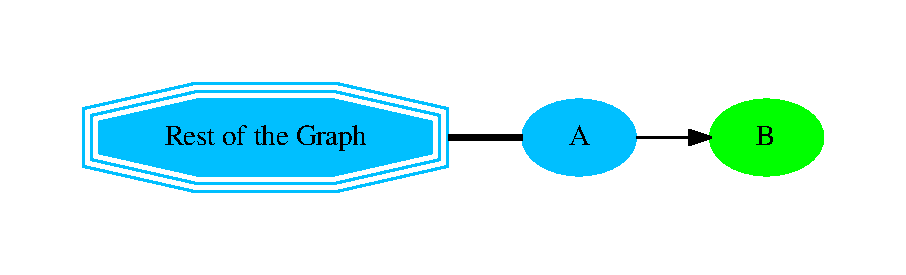
\includegraphics{graphviz-5234bd53dd71aa73dcdf49a40867bf76cd7eeece.pdf}


\paragraph{Operation: Dead End Contraction}
\label{contraction-family:operation-dead-end-contraction}
The dead end contraction will stop until there are no more dead end nodes.
For example from the following graph:
\begin{itemize}
\item {} 
Node \code{A} is connected to the rest of the graph by an unlimited number of edges.

\item {} 
Node \code{B} is connected to the rest of the graph with one incoming edge.

\item {} 
Node \code{B} is the only node connecting to \code{C}.

\item {} 
The green node \code{C} represents a \emph{Dead End} node

\end{itemize}

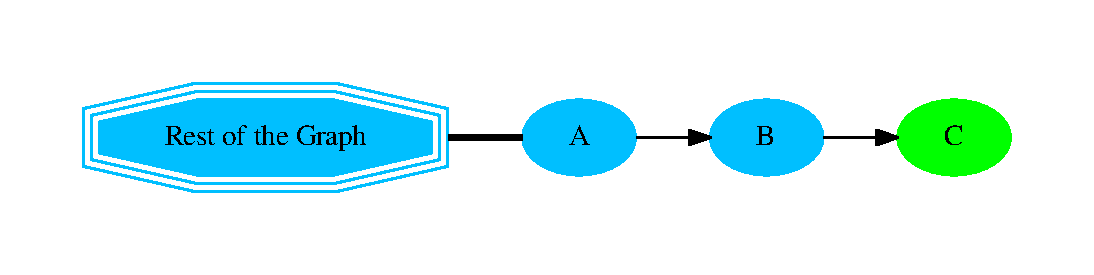
\includegraphics{graphviz-2fc5bee4aea052d2d99303cc04e3d2bd3b719d10.pdf}

After contracting \code{C}, node \code{B} is now a \emph{Dead End} node and is contracted:

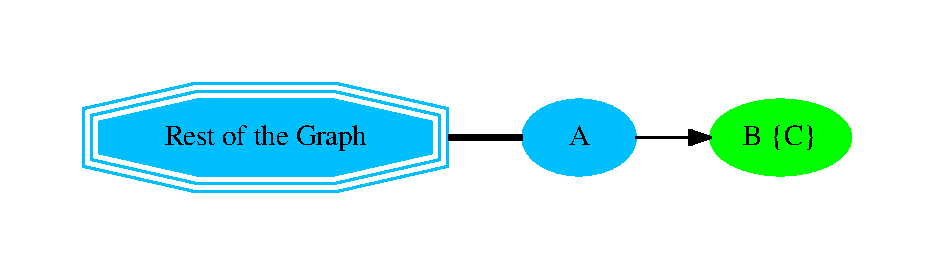
\includegraphics{graphviz-c1fa41046ff4a91086fcef9533739ae0c21423e8.pdf}

Node \code{B} gets contracted

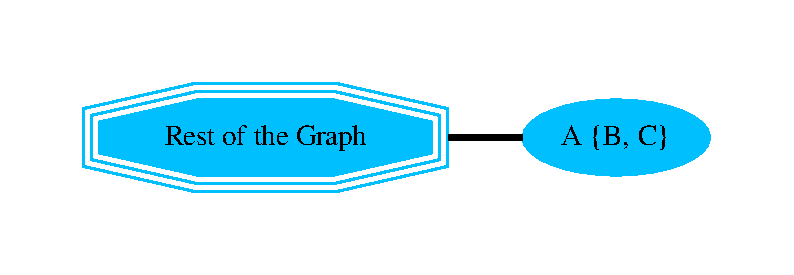
\includegraphics{graphviz-b06b0c770fa8f090fe488e5e05ad95accde5f494.pdf}

Nodes \code{B} and \code{C} belong to node \code{A}.


\paragraph{Not Dead End nodes}
\label{contraction-family:not-dead-end-nodes}
In this graph \code{B} is not a \emph{dead end} node.

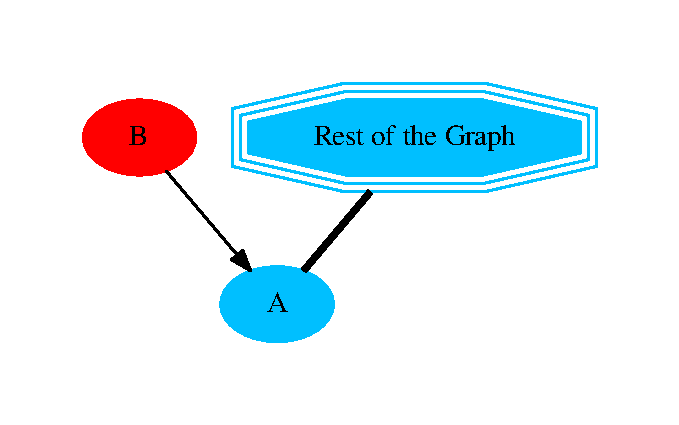
\includegraphics{graphviz-34238e76a3c7511d025e441305a318f778738bfe.pdf}


\subsubsection{Linear contraction}
\label{contraction-family:linear-contraction}
In the algorithm, linear contraction is represented by 2.


\paragraph{Linear nodes}
\label{contraction-family:linear-nodes}
A node is considered a linear node if satisfies the following:
\begin{itemize}
\item {} 
The number of adjacent vertices are 2.

\item {} 
Should have at least one incoming edge and one outgoing edge.

\end{itemize}
\paragraph{Examples}
\begin{itemize}
\item {} 
The green node \code{B} represents a linear node

\item {} 
The nodes \code{A} and \code{C} are the only nodes connecting to \code{B}.

\item {} 
Node \code{A} is part of the rest of the graph and has an unlimited number of incoming and outgoing edges.

\item {} 
Node \code{C} is part of the rest of the graph and has an unlimited number of incoming and outgoing edges.

\item {} 
Directed graph

\end{itemize}

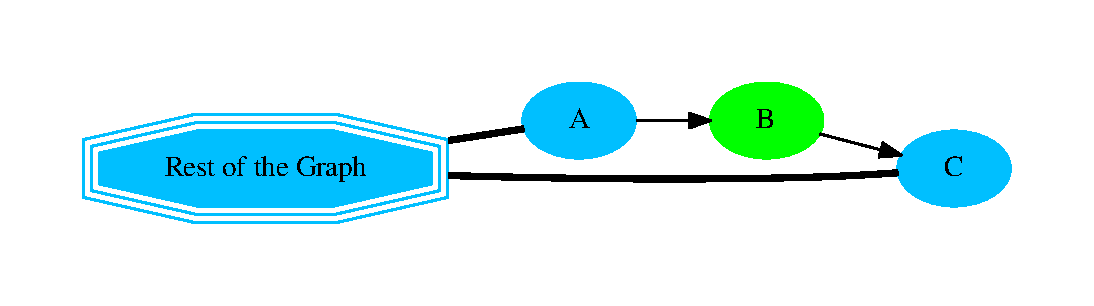
\includegraphics{graphviz-6a336f179d0b0145fe69070034f6227227050025.pdf}


\paragraph{Operation: Linear Contraction}
\label{contraction-family:operation-linear-contraction}
The linear contraction will stop until there are no more linear nodes.
For example from the following graph:
\begin{itemize}
\item {} 
Node \code{A} is connected to the rest of the graph by an unlimited number of edges.

\item {} 
Node \code{B} is connected to the rest of the graph with one incoming edge and one outgoing edge.

\item {} 
Node \code{C} is connected to the rest of the graph with one incoming edge and one outgoing edge.

\item {} 
Node \code{D} is connected to the rest of the graph by an unlimited number of edges.

\item {} 
The green nodes \code{B} and \code{C} represents \emph{Linear} nodes.

\end{itemize}

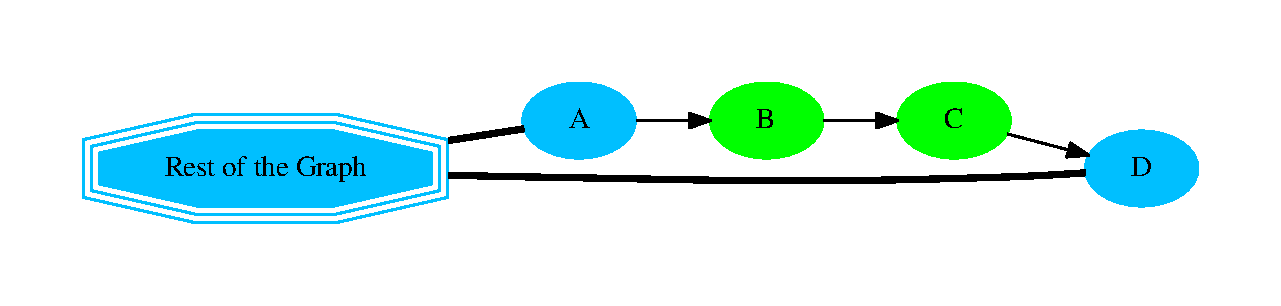
\includegraphics{graphviz-ecc4fb2219f4664e6a65401d4248e7fbed6cc8a5.pdf}

After contracting \code{B}, a new edge gets inserted between \code{A} and \code{C} which is represented by red color.

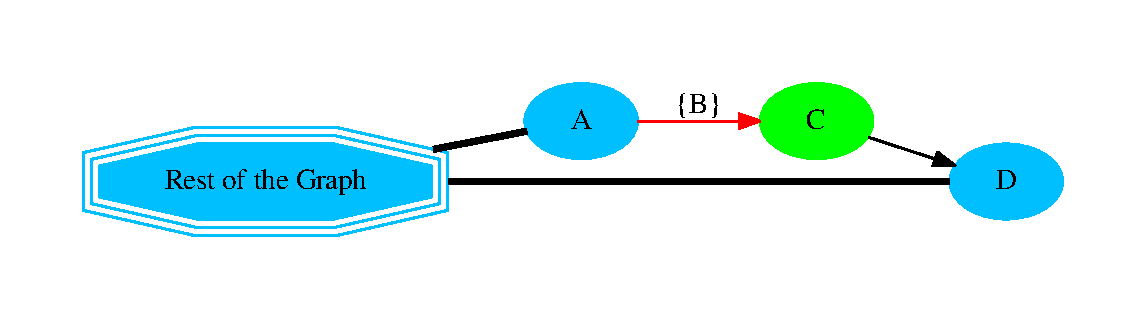
\includegraphics{graphviz-d4a7d13cd6b20a3317ca8decd49284c6cfe2cc6d.pdf}

Node \code{C} is \emph{linear node} and gets contracted.

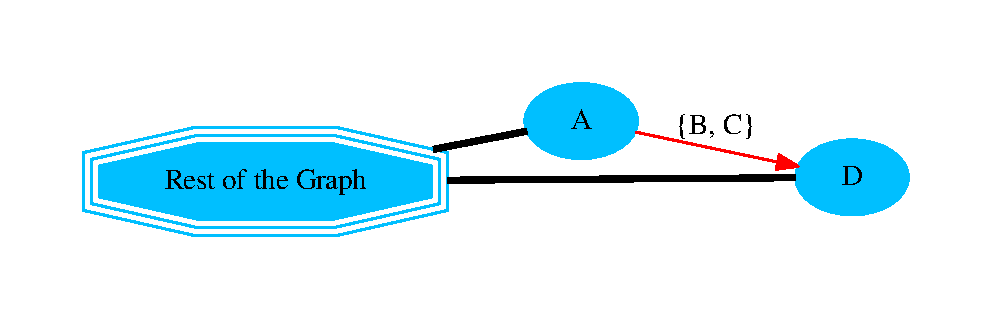
\includegraphics{graphviz-670a660fa776683b3a296840290d645cdc970e32.pdf}

Nodes \code{B} and \code{C} belong to edge connecting \code{A} and \code{D} which is represented by red color.


\paragraph{Not Linear nodes}
\label{contraction-family:not-linear-nodes}
In this graph \code{B} is not a \emph{linear} node.

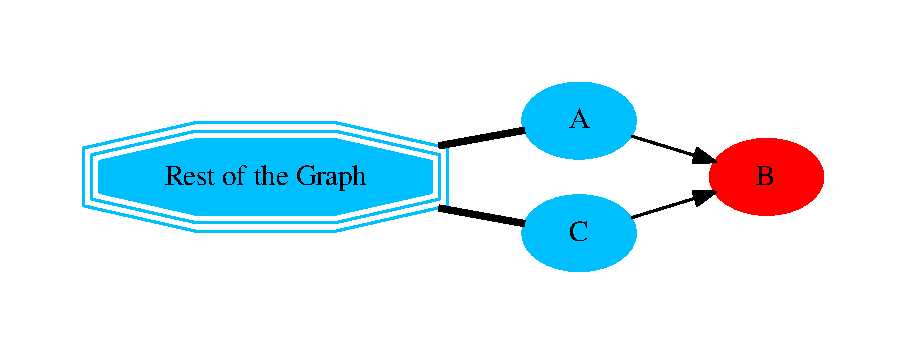
\includegraphics{graphviz-033a3e1eb36d086bdf7edd1d02d4a6687beb9c8d.pdf}


\subsubsection{The cycle}
\label{contraction-family:the-cycle}
Contracting a graph, can be done with more than one operation. The order of the operations affect the resulting contracted graph, after applying one operation, the set of vertices that can be contracted by another operation changes.

This implementation, cycles \code{max\_cycles} times through \code{operations\_order} .

\begin{Verbatim}[commandchars=\\\{\}]
\PYGZlt{}input\PYGZgt{}
do max\PYGZus{}cycles times \PYGZob{}
    for (operation in operations\PYGZus{}order)
     \PYGZob{} do operation \PYGZcb{}
\PYGZcb{}
\PYGZlt{}output\PYGZgt{}
\end{Verbatim}


\subsubsection{Contracting Sample Data}
\label{contraction-family:contracting-sample-data}
In this section, building and using a contracted graph will be shown by example.
\begin{itemize}
\item {} 
The {\hyperref[sampledata::doc]{\emph{\emph{Sample Data}}}} for an undirected graph is used

\item {} 
a dead end operation first followed by a linear operation.

\end{itemize}

The original graph:

\includegraphics{{undirected_sampledata_a}.png}

After doing a dead end contraction operation:

\includegraphics{{undirected_sampledata_b}.png}

Doing a linear contraction operation to the graph above

\includegraphics{{undirected_sampledata_c}.png}

There are five cases, in this documentation, which arise when calculating the shortest path between a given source and target.
In this examples, \code{pgr\_dijkstra} is used.
\begin{itemize}
\item {} 
\textbf{Case 1}: Both source and target belong to the contracted graph.

\item {} 
\textbf{Case 2}: Source belongs to a contracted graph, while target belongs to a edge subgraph.

\item {} 
\textbf{Case 3}: Source belongs to a vertex subgraph, while target belongs to an edge subgraph.

\item {} 
\textbf{Case 4}: Source belongs to a contracted graph, while target belongs to an vertex subgraph.

\item {} 
\textbf{Case 5}: The path contains a new edge added by the contraction algorithm.

\end{itemize}


\paragraph{Construction of the graph in the database}
\label{contraction-family:construction-of-the-graph-in-the-database}\paragraph{Original Data}

The following query shows the original data involved in the contraction operation.

\begin{Verbatim}[commandchars=\\\{\}]

\end{Verbatim}
\paragraph{Contraction Results}

\begin{Verbatim}[commandchars=\\\{\}]
SELECT * FROM pgr\PYGZus{}contractGraph(
    \PYGZsq{}SELECT id, source, target, cost, reverse\PYGZus{}cost FROM edge\PYGZus{}table\PYGZsq{},
    array[1,2], directed:=true);
 seq \textbar{} type \textbar{} id \textbar{} contracted\PYGZus{}vertices \textbar{} source \textbar{} target \textbar{} cost
\PYGZhy{}\PYGZhy{}\PYGZhy{}\PYGZhy{}\PYGZhy{}+\PYGZhy{}\PYGZhy{}\PYGZhy{}\PYGZhy{}\PYGZhy{}\PYGZhy{}+\PYGZhy{}\PYGZhy{}\PYGZhy{}\PYGZhy{}+\PYGZhy{}\PYGZhy{}\PYGZhy{}\PYGZhy{}\PYGZhy{}\PYGZhy{}\PYGZhy{}\PYGZhy{}\PYGZhy{}\PYGZhy{}\PYGZhy{}\PYGZhy{}\PYGZhy{}\PYGZhy{}\PYGZhy{}\PYGZhy{}\PYGZhy{}\PYGZhy{}\PYGZhy{}\PYGZhy{}\PYGZhy{}+\PYGZhy{}\PYGZhy{}\PYGZhy{}\PYGZhy{}\PYGZhy{}\PYGZhy{}\PYGZhy{}\PYGZhy{}+\PYGZhy{}\PYGZhy{}\PYGZhy{}\PYGZhy{}\PYGZhy{}\PYGZhy{}\PYGZhy{}\PYGZhy{}+\PYGZhy{}\PYGZhy{}\PYGZhy{}\PYGZhy{}\PYGZhy{}\PYGZhy{}
   1 \textbar{} v    \textbar{}  5 \textbar{} \PYGZob{}7,8\PYGZcb{}               \textbar{}     \PYGZhy{}1 \textbar{}     \PYGZhy{}1 \textbar{}   \PYGZhy{}1
   2 \textbar{} v    \textbar{} 15 \textbar{} \PYGZob{}14\PYGZcb{}                \textbar{}     \PYGZhy{}1 \textbar{}     \PYGZhy{}1 \textbar{}   \PYGZhy{}1
   3 \textbar{} v    \textbar{} 17 \textbar{} \PYGZob{}16\PYGZcb{}                \textbar{}     \PYGZhy{}1 \textbar{}     \PYGZhy{}1 \textbar{}   \PYGZhy{}1
   4 \textbar{} e    \textbar{} \PYGZhy{}1 \textbar{} \PYGZob{}1,2\PYGZcb{}               \textbar{}      3 \textbar{}      5 \textbar{}    2
   5 \textbar{} e    \textbar{} \PYGZhy{}2 \textbar{} \PYGZob{}4\PYGZcb{}                 \textbar{}      9 \textbar{}      3 \textbar{}    2
   6 \textbar{} e    \textbar{} \PYGZhy{}3 \textbar{} \PYGZob{}10,13\PYGZcb{}             \textbar{}      5 \textbar{}     11 \textbar{}    2
   7 \textbar{} e    \textbar{} \PYGZhy{}4 \textbar{} \PYGZob{}12\PYGZcb{}                \textbar{}     11 \textbar{}      9 \textbar{}    2
(7 rows)

\end{Verbatim}

The above results do not represent the contracted graph. They represent the changes done to the graph after applying the contraction algorithm. We can see that vertices like 6 and 11 do not appear in the contraction results because they were not affected by the contraction algorithm.
\paragraph{step 1}

Adding extra columns to the \code{edge\_table} and \code{edge\_table\_vertices\_pgr} tables:

\begin{tabulary}{\linewidth}{|L|L|}
\hline
\textsf{\relax 
Column
} & \textsf{\relax 
Description
}\\
\hline
\textbf{contracted\_vertices}
 & 
The vertices set belonging to the vertex/edge
\\
\hline
\textbf{is\_contracted}
 & 
On a \emph{vertex} table: when \code{true} the vertex is contracted, so is not part of the contracted graph.
\\
\hline
\textbf{is\_contracted}
 & 
On an \emph{edge} table: when \code{true} the edge was generated by the contraction algorithm.
\\
\hline\end{tabulary}


Using the following queries:

\begin{Verbatim}[commandchars=\\\{\}]
ALTER TABLE edge\PYGZus{}table ADD contracted\PYGZus{}vertices BIGINT[];
ALTER TABLE
ALTER TABLE edge\PYGZus{}table\PYGZus{}vertices\PYGZus{}pgr ADD contracted\PYGZus{}vertices BIGINT[];
ALTER TABLE
ALTER TABLE edge\PYGZus{}table ADD is\PYGZus{}contracted BOOLEAN DEFAULT false;
ALTER TABLE
ALTER TABLE edge\PYGZus{}table\PYGZus{}vertices\PYGZus{}pgr ADD is\PYGZus{}contracted BOOLEAN DEFAULT false;
ALTER TABLE
SET client\PYGZus{}min\PYGZus{}messages TO NOTICE;
SET
\end{Verbatim}
\paragraph{step 2}

For simplicity, in this documentation, store the results of the call to pgr\_contractGraph in a temporary table

\begin{Verbatim}[commandchars=\\\{\}]
SELECT * INTO contraction\PYGZus{}results
FROM pgr\PYGZus{}contractGraph(
    \PYGZsq{}SELECT id, source, target, cost, reverse\PYGZus{}cost FROM edge\PYGZus{}table\PYGZsq{},
    array[1,2], directed:=true);
SELECT 7
\end{Verbatim}
\paragraph{step 3}

Update the \emph{vertex} and \emph{edge} tables using the results of the call to pgr\_contraction
\begin{itemize}
\item {} 
In \emph{edge\_table\_vertices\_pgr.is\_contracted} indicate the vertices that are contracted.

\end{itemize}

\begin{Verbatim}[commandchars=\\\{\}]
UPDATE edge\PYGZus{}table\PYGZus{}vertices\PYGZus{}pgr
SET is\PYGZus{}contracted = true
WHERE id IN (SELECT  unnest(contracted\PYGZus{}vertices) FROM  contraction\PYGZus{}results);
UPDATE 10
\end{Verbatim}
\begin{itemize}
\item {} 
Add to \emph{edge\_table\_vertices\_pgr.contracted\_vertices}  the contracted vertices belonging to the vertices.

\end{itemize}

\begin{Verbatim}[commandchars=\\\{\}]
UPDATE edge\PYGZus{}table\PYGZus{}vertices\PYGZus{}pgr
SET contracted\PYGZus{}vertices = contraction\PYGZus{}results.contracted\PYGZus{}vertices
FROM contraction\PYGZus{}results
WHERE type = \PYGZsq{}v\PYGZsq{} AND edge\PYGZus{}table\PYGZus{}vertices\PYGZus{}pgr.id = contraction\PYGZus{}results.id;
UPDATE 3
\end{Verbatim}
\begin{itemize}
\item {} 
Insert the new edges generated by  pgr\_contractGraph.

\end{itemize}

\begin{Verbatim}[commandchars=\\\{\}]
INSERT INTO edge\PYGZus{}table(source, target, cost, reverse\PYGZus{}cost, contracted\PYGZus{}vertices, is\PYGZus{}contracted)
SELECT source, target, cost, \PYGZhy{}1, contracted\PYGZus{}vertices, true
FROM contraction\PYGZus{}results
WHERE type = \PYGZsq{}e\PYGZsq{};
INSERT 0 4
\end{Verbatim}
\paragraph{step 3.1}

Verify visually the updates.
\begin{itemize}
\item {} 
On the \emph{edge\_table\_vertices\_pgr}

\end{itemize}

\begin{Verbatim}[commandchars=\\\{\}]
SELECT id, contracted\PYGZus{}vertices, is\PYGZus{}contracted
FROM edge\PYGZus{}table\PYGZus{}vertices\PYGZus{}pgr
ORDER BY id;
 id \textbar{} contracted\PYGZus{}vertices \textbar{} is\PYGZus{}contracted
\PYGZhy{}\PYGZhy{}\PYGZhy{}\PYGZhy{}+\PYGZhy{}\PYGZhy{}\PYGZhy{}\PYGZhy{}\PYGZhy{}\PYGZhy{}\PYGZhy{}\PYGZhy{}\PYGZhy{}\PYGZhy{}\PYGZhy{}\PYGZhy{}\PYGZhy{}\PYGZhy{}\PYGZhy{}\PYGZhy{}\PYGZhy{}\PYGZhy{}\PYGZhy{}\PYGZhy{}\PYGZhy{}+\PYGZhy{}\PYGZhy{}\PYGZhy{}\PYGZhy{}\PYGZhy{}\PYGZhy{}\PYGZhy{}\PYGZhy{}\PYGZhy{}\PYGZhy{}\PYGZhy{}\PYGZhy{}\PYGZhy{}\PYGZhy{}\PYGZhy{}
  1 \textbar{}                     \textbar{} t
  2 \textbar{}                     \textbar{} t
  3 \textbar{}                     \textbar{} f
  4 \textbar{}                     \textbar{} t
  5 \textbar{} \PYGZob{}7,8\PYGZcb{}               \textbar{} f
  6 \textbar{}                     \textbar{} f
  7 \textbar{}                     \textbar{} t
  8 \textbar{}                     \textbar{} t
  9 \textbar{}                     \textbar{} f
 10 \textbar{}                     \textbar{} t
 11 \textbar{}                     \textbar{} f
 12 \textbar{}                     \textbar{} t
 13 \textbar{}                     \textbar{} t
 14 \textbar{}                     \textbar{} t
 15 \textbar{} \PYGZob{}14\PYGZcb{}                \textbar{} f
 16 \textbar{}                     \textbar{} t
 17 \textbar{} \PYGZob{}16\PYGZcb{}                \textbar{} f
(17 rows)

\end{Verbatim}
\begin{itemize}
\item {} 
On the \emph{edge\_table}

\end{itemize}

\begin{Verbatim}[commandchars=\\\{\}]
SELECT id, source, target, cost, reverse\PYGZus{}cost, contracted\PYGZus{}vertices, is\PYGZus{}contracted
FROM edge\PYGZus{}table
ORDER BY id;
 id \textbar{} source \textbar{} target \textbar{} cost \textbar{} reverse\PYGZus{}cost \textbar{} contracted\PYGZus{}vertices \textbar{} is\PYGZus{}contracted
\PYGZhy{}\PYGZhy{}\PYGZhy{}\PYGZhy{}+\PYGZhy{}\PYGZhy{}\PYGZhy{}\PYGZhy{}\PYGZhy{}\PYGZhy{}\PYGZhy{}\PYGZhy{}+\PYGZhy{}\PYGZhy{}\PYGZhy{}\PYGZhy{}\PYGZhy{}\PYGZhy{}\PYGZhy{}\PYGZhy{}+\PYGZhy{}\PYGZhy{}\PYGZhy{}\PYGZhy{}\PYGZhy{}\PYGZhy{}+\PYGZhy{}\PYGZhy{}\PYGZhy{}\PYGZhy{}\PYGZhy{}\PYGZhy{}\PYGZhy{}\PYGZhy{}\PYGZhy{}\PYGZhy{}\PYGZhy{}\PYGZhy{}\PYGZhy{}\PYGZhy{}+\PYGZhy{}\PYGZhy{}\PYGZhy{}\PYGZhy{}\PYGZhy{}\PYGZhy{}\PYGZhy{}\PYGZhy{}\PYGZhy{}\PYGZhy{}\PYGZhy{}\PYGZhy{}\PYGZhy{}\PYGZhy{}\PYGZhy{}\PYGZhy{}\PYGZhy{}\PYGZhy{}\PYGZhy{}\PYGZhy{}\PYGZhy{}+\PYGZhy{}\PYGZhy{}\PYGZhy{}\PYGZhy{}\PYGZhy{}\PYGZhy{}\PYGZhy{}\PYGZhy{}\PYGZhy{}\PYGZhy{}\PYGZhy{}\PYGZhy{}\PYGZhy{}\PYGZhy{}\PYGZhy{}
  1 \textbar{}      1 \textbar{}      2 \textbar{}    1 \textbar{}            1 \textbar{}                     \textbar{} f
  2 \textbar{}      2 \textbar{}      3 \textbar{}   \PYGZhy{}1 \textbar{}            1 \textbar{}                     \textbar{} f
  3 \textbar{}      3 \textbar{}      4 \textbar{}   \PYGZhy{}1 \textbar{}            1 \textbar{}                     \textbar{} f
  4 \textbar{}      2 \textbar{}      5 \textbar{}    1 \textbar{}            1 \textbar{}                     \textbar{} f
  5 \textbar{}      3 \textbar{}      6 \textbar{}    1 \textbar{}           \PYGZhy{}1 \textbar{}                     \textbar{} f
  6 \textbar{}      7 \textbar{}      8 \textbar{}    1 \textbar{}            1 \textbar{}                     \textbar{} f
  7 \textbar{}      8 \textbar{}      5 \textbar{}    1 \textbar{}            1 \textbar{}                     \textbar{} f
  8 \textbar{}      5 \textbar{}      6 \textbar{}    1 \textbar{}            1 \textbar{}                     \textbar{} f
  9 \textbar{}      6 \textbar{}      9 \textbar{}    1 \textbar{}            1 \textbar{}                     \textbar{} f
 10 \textbar{}      5 \textbar{}     10 \textbar{}    1 \textbar{}            1 \textbar{}                     \textbar{} f
 11 \textbar{}      6 \textbar{}     11 \textbar{}    1 \textbar{}           \PYGZhy{}1 \textbar{}                     \textbar{} f
 12 \textbar{}     10 \textbar{}     11 \textbar{}    1 \textbar{}           \PYGZhy{}1 \textbar{}                     \textbar{} f
 13 \textbar{}     11 \textbar{}     12 \textbar{}    1 \textbar{}           \PYGZhy{}1 \textbar{}                     \textbar{} f
 14 \textbar{}     10 \textbar{}     13 \textbar{}    1 \textbar{}            1 \textbar{}                     \textbar{} f
 15 \textbar{}      9 \textbar{}     12 \textbar{}    1 \textbar{}            1 \textbar{}                     \textbar{} f
 16 \textbar{}      4 \textbar{}      9 \textbar{}    1 \textbar{}            1 \textbar{}                     \textbar{} f
 17 \textbar{}     14 \textbar{}     15 \textbar{}    1 \textbar{}            1 \textbar{}                     \textbar{} f
 18 \textbar{}     16 \textbar{}     17 \textbar{}    1 \textbar{}            1 \textbar{}                     \textbar{} f
 19 \textbar{}      3 \textbar{}      5 \textbar{}    2 \textbar{}           \PYGZhy{}1 \textbar{} \PYGZob{}1,2\PYGZcb{}               \textbar{} t
 20 \textbar{}      9 \textbar{}      3 \textbar{}    2 \textbar{}           \PYGZhy{}1 \textbar{} \PYGZob{}4\PYGZcb{}                 \textbar{} t
 21 \textbar{}      5 \textbar{}     11 \textbar{}    2 \textbar{}           \PYGZhy{}1 \textbar{} \PYGZob{}10,13\PYGZcb{}             \textbar{} t
 22 \textbar{}     11 \textbar{}      9 \textbar{}    2 \textbar{}           \PYGZhy{}1 \textbar{} \PYGZob{}12\PYGZcb{}                \textbar{} t
(22 rows)

\end{Verbatim}
\begin{itemize}
\item {} 
vertices that belong to the contracted graph are the non contracted vertices

\end{itemize}

\begin{Verbatim}[commandchars=\\\{\}]
SELECT id  FROM edge\PYGZus{}table\PYGZus{}vertices\PYGZus{}pgr
WHERE is\PYGZus{}contracted = false
ORDER BY id;
 id
\PYGZhy{}\PYGZhy{}\PYGZhy{}\PYGZhy{}
  3
  5
  6
  9
 11
 15
 17
(7 rows)

\end{Verbatim}
\paragraph{case 1: Both source and target belong to the contracted graph.}

Inspecting the contracted graph above, vertex 3 and vertex 11 are part of the contracted graph. In the following query:
\begin{itemize}
\item {} 
vertices\_in\_graph hold the vertices that belong to the contracted graph.

\item {} 
when selecting the edges, only edges that have the source and the target in that set are the edges belonging to the contracted graph, that is done in the WHERE clause.

\end{itemize}

Visually, looking at the original graph, going from 3 to 11: 3 -\textgreater{} 6 -\textgreater{} 11, and in the contracted graph, it is also 3 -\textgreater{} 6 -\textgreater{} 11.
The results, on the contracted graph match the results as if it was done on the original graph.

\begin{Verbatim}[commandchars=\\\{\}]
SELECT * FROM pgr\PYGZus{}dijkstra(
    \PYGZdl{}\PYGZdl{}
    WITH
    vertices\PYGZus{}in\PYGZus{}graph AS (
        SELECT id  FROM edge\PYGZus{}table\PYGZus{}vertices\PYGZus{}pgr WHERE is\PYGZus{}contracted = false)
    SELECT id, source, target, cost, reverse\PYGZus{}cost
    FROM edge\PYGZus{}table
    WHERE source IN (SELECT * FROM vertices\PYGZus{}in\PYGZus{}graph)
    AND target IN (SELECT * FROM vertices\PYGZus{}in\PYGZus{}graph)
    \PYGZdl{}\PYGZdl{},
    3, 11, false);
 seq \textbar{} path\PYGZus{}seq \textbar{} node \textbar{} edge \textbar{} cost \textbar{} agg\PYGZus{}cost
\PYGZhy{}\PYGZhy{}\PYGZhy{}\PYGZhy{}\PYGZhy{}+\PYGZhy{}\PYGZhy{}\PYGZhy{}\PYGZhy{}\PYGZhy{}\PYGZhy{}\PYGZhy{}\PYGZhy{}\PYGZhy{}\PYGZhy{}+\PYGZhy{}\PYGZhy{}\PYGZhy{}\PYGZhy{}\PYGZhy{}\PYGZhy{}+\PYGZhy{}\PYGZhy{}\PYGZhy{}\PYGZhy{}\PYGZhy{}\PYGZhy{}+\PYGZhy{}\PYGZhy{}\PYGZhy{}\PYGZhy{}\PYGZhy{}\PYGZhy{}+\PYGZhy{}\PYGZhy{}\PYGZhy{}\PYGZhy{}\PYGZhy{}\PYGZhy{}\PYGZhy{}\PYGZhy{}\PYGZhy{}\PYGZhy{}
   1 \textbar{}        1 \textbar{}    3 \textbar{}    5 \textbar{}    1 \textbar{}        0
   2 \textbar{}        2 \textbar{}    6 \textbar{}   11 \textbar{}    1 \textbar{}        1
   3 \textbar{}        3 \textbar{}   11 \textbar{}   \PYGZhy{}1 \textbar{}    0 \textbar{}        2
(3 rows)

\end{Verbatim}
\paragraph{case 2: Source belongs to the contracted graph, while target belongs to a edge subgraph.}
\begin{description}
\item[{Inspecting the contracted graph above, vertex 3 is part of the contracted graph and vertex 1 belongs to the contracted subgraph of edge 19. In the following query:}] \leavevmode\begin{itemize}
\item {} 
expand1 holds the contracted vertices of the edge where vertex 1 belongs. (belongs to edge 19).

\item {} 
vertices\_in\_graph hold the vertices that belong to the contracted graph and also the contracted vertices of edge 19.

\item {} 
when selecting the edges, only edges that have the source and the target in that set are the edges belonging to the contracted graph, that is done in the WHERE clause.

\end{itemize}

\end{description}

Visually, looking at the original graph, going from 3 to 1: 3 -\textgreater{} 2 -\textgreater{} 1, and in the contracted graph, it is also 3 -\textgreater{} 2 -\textgreater{} 1.
The results, on the contracted graph match the results as if it was done on the original graph.

\begin{Verbatim}[commandchars=\\\{\}]
SELECT * FROM pgr\PYGZus{}dijkstra(
    \PYGZdl{}\PYGZdl{}
    WITH
    expand\PYGZus{}edges AS (SELECT id, unnest(contracted\PYGZus{}vertices) AS vertex FROM edge\PYGZus{}table),
    expand1 AS (SELECT contracted\PYGZus{}vertices FROM edge\PYGZus{}table
        WHERE id IN (SELECT id FROM expand\PYGZus{}edges WHERE vertex = 1)),
    vertices\PYGZus{}in\PYGZus{}graph AS (
        SELECT id  FROM edge\PYGZus{}table\PYGZus{}vertices\PYGZus{}pgr WHERE is\PYGZus{}contracted = false
        UNION
        SELECT unnest(contracted\PYGZus{}vertices) FROM expand1)
    SELECT id, source, target, cost, reverse\PYGZus{}cost
    FROM edge\PYGZus{}table
    WHERE source IN (SELECT * FROM vertices\PYGZus{}in\PYGZus{}graph)
    AND target IN (SELECT * FROM vertices\PYGZus{}in\PYGZus{}graph)
    \PYGZdl{}\PYGZdl{},
    3, 1, false);
 seq \textbar{} path\PYGZus{}seq \textbar{} node \textbar{} edge \textbar{} cost \textbar{} agg\PYGZus{}cost
\PYGZhy{}\PYGZhy{}\PYGZhy{}\PYGZhy{}\PYGZhy{}+\PYGZhy{}\PYGZhy{}\PYGZhy{}\PYGZhy{}\PYGZhy{}\PYGZhy{}\PYGZhy{}\PYGZhy{}\PYGZhy{}\PYGZhy{}+\PYGZhy{}\PYGZhy{}\PYGZhy{}\PYGZhy{}\PYGZhy{}\PYGZhy{}+\PYGZhy{}\PYGZhy{}\PYGZhy{}\PYGZhy{}\PYGZhy{}\PYGZhy{}+\PYGZhy{}\PYGZhy{}\PYGZhy{}\PYGZhy{}\PYGZhy{}\PYGZhy{}+\PYGZhy{}\PYGZhy{}\PYGZhy{}\PYGZhy{}\PYGZhy{}\PYGZhy{}\PYGZhy{}\PYGZhy{}\PYGZhy{}\PYGZhy{}
   1 \textbar{}        1 \textbar{}    3 \textbar{}    2 \textbar{}    1 \textbar{}        0
   2 \textbar{}        2 \textbar{}    2 \textbar{}    1 \textbar{}    1 \textbar{}        1
   3 \textbar{}        3 \textbar{}    1 \textbar{}   \PYGZhy{}1 \textbar{}    0 \textbar{}        2
(3 rows)

\end{Verbatim}
\paragraph{case 3: Source belongs to a vertex subgraph, while target belongs to an edge subgraph.}

Inspecting the contracted graph above, vertex 7 belongs to the contracted subgraph of vertex 5 and vertex 13 belongs to the contracted subgraph of edge 21. In the following query:
\begin{itemize}
\item {} 
expand7 holds the contracted vertices of vertex where vertex 7 belongs. (belongs to vertex 5)

\item {} 
expand13 holds the contracted vertices of edge where vertex 13 belongs. (belongs to edge 21)

\item {} 
vertices\_in\_graph hold the vertices that belong to the contracted graph, contracted vertices of vertex 5 and contracted vertices of edge 21.

\item {} 
when selecting the edges, only edges that have the source and the target in that set are the edges belonging to the contracted graph, that is done in the WHERE clause.

\end{itemize}

Visually, looking at the original graph, going from 7 to 13: 7 -\textgreater{} 8 -\textgreater{} 5 -\textgreater{} 10 -\textgreater{} 13, and in the contracted graph, it is also 7 -\textgreater{} 8 -\textgreater{} 5 -\textgreater{} 10 -\textgreater{} 13.
The results, on the contracted graph match the results as if it was done on the original graph.

\begin{Verbatim}[commandchars=\\\{\}]
SELECT * FROM pgr\PYGZus{}dijkstra(
    \PYGZdl{}\PYGZdl{}
    WITH

    expand\PYGZus{}vertices AS (SELECT id, unnest(contracted\PYGZus{}vertices) AS vertex FROM edge\PYGZus{}table\PYGZus{}vertices\PYGZus{}pgr),
    expand7 AS (SELECT contracted\PYGZus{}vertices FROM edge\PYGZus{}table\PYGZus{}vertices\PYGZus{}pgr
        WHERE id IN (SELECT id FROM expand\PYGZus{}vertices WHERE vertex = 7)),

    expand\PYGZus{}edges AS (SELECT id, unnest(contracted\PYGZus{}vertices) AS vertex FROM edge\PYGZus{}table),
    expand13 AS (SELECT contracted\PYGZus{}vertices FROM edge\PYGZus{}table
        WHERE id IN (SELECT id FROM expand\PYGZus{}edges WHERE vertex = 13)),

    vertices\PYGZus{}in\PYGZus{}graph AS (
        SELECT id  FROM edge\PYGZus{}table\PYGZus{}vertices\PYGZus{}pgr WHERE is\PYGZus{}contracted = false
        UNION
        SELECT unnest(contracted\PYGZus{}vertices) FROM expand13
        UNION
        SELECT unnest(contracted\PYGZus{}vertices) FROM expand7)

    SELECT id, source, target, cost, reverse\PYGZus{}cost
    FROM edge\PYGZus{}table
    WHERE source IN (SELECT * FROM vertices\PYGZus{}in\PYGZus{}graph)
    AND target IN (SELECT * FROM vertices\PYGZus{}in\PYGZus{}graph)
    \PYGZdl{}\PYGZdl{},
    7, 13, false);
 seq \textbar{} path\PYGZus{}seq \textbar{} node \textbar{} edge \textbar{} cost \textbar{} agg\PYGZus{}cost
\PYGZhy{}\PYGZhy{}\PYGZhy{}\PYGZhy{}\PYGZhy{}+\PYGZhy{}\PYGZhy{}\PYGZhy{}\PYGZhy{}\PYGZhy{}\PYGZhy{}\PYGZhy{}\PYGZhy{}\PYGZhy{}\PYGZhy{}+\PYGZhy{}\PYGZhy{}\PYGZhy{}\PYGZhy{}\PYGZhy{}\PYGZhy{}+\PYGZhy{}\PYGZhy{}\PYGZhy{}\PYGZhy{}\PYGZhy{}\PYGZhy{}+\PYGZhy{}\PYGZhy{}\PYGZhy{}\PYGZhy{}\PYGZhy{}\PYGZhy{}+\PYGZhy{}\PYGZhy{}\PYGZhy{}\PYGZhy{}\PYGZhy{}\PYGZhy{}\PYGZhy{}\PYGZhy{}\PYGZhy{}\PYGZhy{}
   1 \textbar{}        1 \textbar{}    7 \textbar{}    6 \textbar{}    1 \textbar{}        0
   2 \textbar{}        2 \textbar{}    8 \textbar{}    7 \textbar{}    1 \textbar{}        1
   3 \textbar{}        3 \textbar{}    5 \textbar{}   10 \textbar{}    1 \textbar{}        2
   4 \textbar{}        4 \textbar{}   10 \textbar{}   14 \textbar{}    1 \textbar{}        3
   5 \textbar{}        5 \textbar{}   13 \textbar{}   \PYGZhy{}1 \textbar{}    0 \textbar{}        4
(5 rows)

\end{Verbatim}
\paragraph{case 4: Source belongs to the contracted graph, while target belongs to an vertex subgraph.}

Inspecting the contracted graph above, vertex 3 is part of the contracted graph and vertex 7 belongs to the contracted subgraph of vertex 5. In the following query:
\begin{itemize}
\item {} 
expand7 holds the contracted vertices of vertex where vertex 7 belongs. (belongs to vertex 5)

\item {} 
vertices\_in\_graph hold the vertices that belong to the contracted graph and the contracted vertices of vertex 5.

\item {} 
when selecting the edges, only edges that have the source and the target in that set are the edges belonging to the contracted graph, that is done in the WHERE clause.

\end{itemize}

Visually, looking at the original graph, going from 3 to 7: 3 -\textgreater{} 2 -\textgreater{} 5 -\textgreater{} 8 -\textgreater{} 7, but in the contracted graph, it is 3 -\textgreater{} 5 -\textgreater{} 8 -\textgreater{} 7.
The results, on the contracted graph do not match the results as if it was done on the original graph. This is because the path contains edge 19 which is added by the contraction algorithm.

\begin{Verbatim}[commandchars=\\\{\}]
SELECT * FROM  pgr\PYGZus{}dijkstra(
    \PYGZdl{}\PYGZdl{}
    WITH
    expand\PYGZus{}vertices AS (SELECT id, unnest(contracted\PYGZus{}vertices) AS vertex FROM edge\PYGZus{}table\PYGZus{}vertices\PYGZus{}pgr),
    expand7 AS (SELECT contracted\PYGZus{}vertices FROM edge\PYGZus{}table\PYGZus{}vertices\PYGZus{}pgr
        WHERE id IN (SELECT id FROM expand\PYGZus{}vertices WHERE vertex = 7)),
    vertices\PYGZus{}in\PYGZus{}graph AS (
        SELECT id  FROM edge\PYGZus{}table\PYGZus{}vertices\PYGZus{}pgr WHERE is\PYGZus{}contracted = false
        UNION
        SELECT unnest(contracted\PYGZus{}vertices) FROM expand7)
    SELECT id, source, target, cost, reverse\PYGZus{}cost
    FROM edge\PYGZus{}table
    WHERE source IN (SELECT * FROM vertices\PYGZus{}in\PYGZus{}graph)
    AND target IN (SELECT * FROM vertices\PYGZus{}in\PYGZus{}graph)
    \PYGZdl{}\PYGZdl{},
    3, 7, false);
 seq \textbar{} path\PYGZus{}seq \textbar{} node \textbar{} edge \textbar{} cost \textbar{} agg\PYGZus{}cost
\PYGZhy{}\PYGZhy{}\PYGZhy{}\PYGZhy{}\PYGZhy{}+\PYGZhy{}\PYGZhy{}\PYGZhy{}\PYGZhy{}\PYGZhy{}\PYGZhy{}\PYGZhy{}\PYGZhy{}\PYGZhy{}\PYGZhy{}+\PYGZhy{}\PYGZhy{}\PYGZhy{}\PYGZhy{}\PYGZhy{}\PYGZhy{}+\PYGZhy{}\PYGZhy{}\PYGZhy{}\PYGZhy{}\PYGZhy{}\PYGZhy{}+\PYGZhy{}\PYGZhy{}\PYGZhy{}\PYGZhy{}\PYGZhy{}\PYGZhy{}+\PYGZhy{}\PYGZhy{}\PYGZhy{}\PYGZhy{}\PYGZhy{}\PYGZhy{}\PYGZhy{}\PYGZhy{}\PYGZhy{}\PYGZhy{}
   1 \textbar{}        1 \textbar{}    3 \textbar{}   19 \textbar{}    2 \textbar{}        0
   2 \textbar{}        2 \textbar{}    5 \textbar{}    7 \textbar{}    1 \textbar{}        2
   3 \textbar{}        3 \textbar{}    8 \textbar{}    6 \textbar{}    1 \textbar{}        3
   4 \textbar{}        4 \textbar{}    7 \textbar{}   \PYGZhy{}1 \textbar{}    0 \textbar{}        4
(4 rows)

\end{Verbatim}
\paragraph{case 5: The path contains an edge added by the contraction algorithm.}

In the previous example we can see that the path from vertex 3 to vertex 7 contains an edge which is added by the contraction algorithm.

\begin{Verbatim}[commandchars=\\\{\}]
WITH
first\PYGZus{}dijkstra AS (
    SELECT * FROM  pgr\PYGZus{}dijkstra(
        \PYGZdl{}\PYGZdl{}
        WITH
        expand\PYGZus{}vertices AS (SELECT id, unnest(contracted\PYGZus{}vertices) AS vertex FROM edge\PYGZus{}table\PYGZus{}vertices\PYGZus{}pgr),
        expand7 AS (SELECT contracted\PYGZus{}vertices FROM edge\PYGZus{}table\PYGZus{}vertices\PYGZus{}pgr
            WHERE id IN (SELECT id FROM expand\PYGZus{}vertices WHERE vertex = 7)),
        vertices\PYGZus{}in\PYGZus{}graph AS (
            SELECT id  FROM edge\PYGZus{}table\PYGZus{}vertices\PYGZus{}pgr WHERE is\PYGZus{}contracted = false
            UNION
            SELECT unnest(contracted\PYGZus{}vertices) FROM expand7)
        SELECT id, source, target, cost, reverse\PYGZus{}cost
        FROM edge\PYGZus{}table
        WHERE source IN (SELECT * FROM vertices\PYGZus{}in\PYGZus{}graph)
        AND target IN (SELECT * FROM vertices\PYGZus{}in\PYGZus{}graph)
        \PYGZdl{}\PYGZdl{},
        3, 7, false))
SELECT edge, contracted\PYGZus{}vertices
    FROM first\PYGZus{}dijkstra JOIN edge\PYGZus{}table
    ON (edge = id)
    WHERE is\PYGZus{}contracted = true;
 edge \textbar{} contracted\PYGZus{}vertices
\PYGZhy{}\PYGZhy{}\PYGZhy{}\PYGZhy{}\PYGZhy{}\PYGZhy{}+\PYGZhy{}\PYGZhy{}\PYGZhy{}\PYGZhy{}\PYGZhy{}\PYGZhy{}\PYGZhy{}\PYGZhy{}\PYGZhy{}\PYGZhy{}\PYGZhy{}\PYGZhy{}\PYGZhy{}\PYGZhy{}\PYGZhy{}\PYGZhy{}\PYGZhy{}\PYGZhy{}\PYGZhy{}\PYGZhy{}\PYGZhy{}
   19 \textbar{} \PYGZob{}1,2\PYGZcb{}
(1 row)

\end{Verbatim}

Inspecting the contracted graph above, edge 19 should be expanded. In the following query:
\begin{itemize}
\item {} 
first\_dijkstra holds the results of the dijkstra query.

\item {} 
edges\_to\_expand holds the edges added by the contraction algorithm and included in the path.

\item {} 
vertices\_in\_graph hold the vertices that belong to the contracted graph, vertices of the contracted solution and the contracted vertices of the edges added by the contraction algorithm and included in the contracted solution.

\item {} 
when selecting the edges, only edges that have the source and the target in that set are the edges belonging to the contracted graph, that is done in the WHERE clause.

\end{itemize}

Visually, looking at the original graph, going from 3 to 7: 3 -\textgreater{} 2 -\textgreater{} 5 -\textgreater{} 8 -\textgreater{} 7, and in the contracted graph, it is also 3 -\textgreater{} 2 -\textgreater{} 5 -\textgreater{} 8 -\textgreater{} 7.
The results, on the contracted graph match the results as if it was done on the original graph.

\begin{Verbatim}[commandchars=\\\{\}]
SELECT * FROM pgr\PYGZus{}dijkstra(\PYGZdl{}\PYGZdl{}
    WITH
    \PYGZhy{}\PYGZhy{} This returns the results from case 2
    first\PYGZus{}dijkstra AS (
        SELECT * FROM  pgr\PYGZus{}dijkstra(
            \PYGZsq{}
            WITH
            expand\PYGZus{}vertices AS (SELECT id, unnest(contracted\PYGZus{}vertices) AS vertex FROM edge\PYGZus{}table\PYGZus{}vertices\PYGZus{}pgr),
            expand7 AS (SELECT contracted\PYGZus{}vertices FROM edge\PYGZus{}table\PYGZus{}vertices\PYGZus{}pgr
                WHERE id IN (SELECT id FROM expand\PYGZus{}vertices WHERE vertex = 7)),
            vertices\PYGZus{}in\PYGZus{}graph AS (
                SELECT id  FROM edge\PYGZus{}table\PYGZus{}vertices\PYGZus{}pgr WHERE is\PYGZus{}contracted = false
                UNION
                SELECT unnest(contracted\PYGZus{}vertices) FROM expand7)
            SELECT id, source, target, cost, reverse\PYGZus{}cost
            FROM edge\PYGZus{}table
            WHERE source IN (SELECT * FROM vertices\PYGZus{}in\PYGZus{}graph)
            AND target IN (SELECT * FROM vertices\PYGZus{}in\PYGZus{}graph)
            \PYGZsq{},
            3, 7, false)),

    \PYGZhy{}\PYGZhy{} edges that need expansion and the vertices to be expanded.
    edges\PYGZus{}to\PYGZus{}expand AS (
        SELECT edge, contracted\PYGZus{}vertices
        FROM first\PYGZus{}dijkstra JOIN edge\PYGZus{}table
        ON (edge = id)
        WHERE is\PYGZus{}contracted = true),

    vertices\PYGZus{}in\PYGZus{}graph AS (
        \PYGZhy{}\PYGZhy{} the nodes of the contracted solution
        SELECT node FROM first\PYGZus{}dijkstra
        UNION
        \PYGZhy{}\PYGZhy{} the nodes of the expanding sections
        SELECT unnest(contracted\PYGZus{}vertices) FROM edges\PYGZus{}to\PYGZus{}expand)

    SELECT id, source, target, cost, reverse\PYGZus{}cost
    FROM edge\PYGZus{}table
    WHERE source IN (SELECT * FROM vertices\PYGZus{}in\PYGZus{}graph)
    AND target IN (SELECT * FROM vertices\PYGZus{}in\PYGZus{}graph)
    \PYGZhy{}\PYGZhy{} not including the expanded edges
    AND id NOT IN (SELECT edge FROM edges\PYGZus{}to\PYGZus{}expand)
    \PYGZdl{}\PYGZdl{},
    3, 7, false);
 seq \textbar{} path\PYGZus{}seq \textbar{} node \textbar{} edge \textbar{} cost \textbar{} agg\PYGZus{}cost
\PYGZhy{}\PYGZhy{}\PYGZhy{}\PYGZhy{}\PYGZhy{}+\PYGZhy{}\PYGZhy{}\PYGZhy{}\PYGZhy{}\PYGZhy{}\PYGZhy{}\PYGZhy{}\PYGZhy{}\PYGZhy{}\PYGZhy{}+\PYGZhy{}\PYGZhy{}\PYGZhy{}\PYGZhy{}\PYGZhy{}\PYGZhy{}+\PYGZhy{}\PYGZhy{}\PYGZhy{}\PYGZhy{}\PYGZhy{}\PYGZhy{}+\PYGZhy{}\PYGZhy{}\PYGZhy{}\PYGZhy{}\PYGZhy{}\PYGZhy{}+\PYGZhy{}\PYGZhy{}\PYGZhy{}\PYGZhy{}\PYGZhy{}\PYGZhy{}\PYGZhy{}\PYGZhy{}\PYGZhy{}\PYGZhy{}
   1 \textbar{}        1 \textbar{}    3 \textbar{}    2 \textbar{}    1 \textbar{}        0
   2 \textbar{}        2 \textbar{}    2 \textbar{}    4 \textbar{}    1 \textbar{}        1
   3 \textbar{}        3 \textbar{}    5 \textbar{}    7 \textbar{}    1 \textbar{}        2
   4 \textbar{}        4 \textbar{}    8 \textbar{}    6 \textbar{}    1 \textbar{}        3
   5 \textbar{}        5 \textbar{}    7 \textbar{}   \PYGZhy{}1 \textbar{}    0 \textbar{}        4
(5 rows)

\end{Verbatim}


\subsubsection{See Also}
\label{contraction-family:see-also}\begin{itemize}
\item {} 
\href{http://www.cs.cmu.edu/afs/cs/academic/class/15210-f12/www/lectures/lecture16.pdf}{http://www.cs.cmu.edu/afs/cs/academic/class/15210-f12/www/lectures/lecture16.pdf}

\item {} 
\href{http://algo2.iti.kit.edu/documents/routeplanning/geisberger\_dipl.pdf}{http://algo2.iti.kit.edu/documents/routeplanning/geisberger\_dipl.pdf}

\item {} 
The queries use {\hyperref[pgr_contractGraph:pgr\string-contractgraph]{\emph{pgr\_contractGraph - Experimental}}} function and the {\hyperref[sampledata::doc]{\emph{\emph{Sample Data}}}} network.

\end{itemize}
\paragraph{Indices and tables}
\begin{itemize}
\item {} 
\DUspan{xref,std,std-ref}{genindex}

\item {} 
\DUspan{xref,std,std-ref}{search}

\end{itemize}


\subsection{Flow - Family of functions}
\label{flow-family:maxflow}\label{flow-family::doc}\label{flow-family:flow-family-of-functions}\begin{itemize}
\item {} 
{\hyperref[pgr_maxFlow:pgr\string-maxflow]{\emph{pgr\_maxFlow - Proposed}}} - Only the Max flow calculation using Push and Relabel algorithm.

\item {} 
{\hyperref[pgr_boykovKolmogorov:pgr\string-boykovkolmogorov]{\emph{pgr\_boykovKolmogorov - Proposed}}} - Boykov and Kolmogorov with details of flow on edges.

\item {} 
{\hyperref[pgr_edmondsKarp:pgr\string-edmondskarp]{\emph{pgr\_edmondsKarp - Proposed}}} - Edmonds and Karp algorithm with details of flow on edges.

\item {} 
{\hyperref[pgr_pushRelabel:pgr\string-pushrelabel]{\emph{pgr\_pushRelabel - Proposed}}} - Push and relabel algorithm with details of flow on edges.

\item {} 
Applications
\begin{itemize}
\item {} 
{\hyperref[pgr_edgeDisjointPaths:pgr\string-edgedisjointpaths]{\emph{pgr\_edgeDisjointPaths - Proposed}}} - Calculates edge disjoint paths between two groups of vertices.

\item {} 
{\hyperref[pgr_maxCardinalityMatch:pgr\string-maxcardinalitymatch]{\emph{pgr\_maxCardinalityMatch - Proposed}}} - Calculates a maximum cardinality matching in a graph.

\end{itemize}

\end{itemize}

\begin{notice}{warning}{Warning:}
Experimental functions
\begin{itemize}
\item {} 
They are not officially of the current release.

\item {} 
They likely will not be officially be part of the next release:
\begin{itemize}
\item {} 
The functions might not make use of ANY-INTEGER and ANY-NUMERICAL

\item {} 
Name might change.

\item {} 
Signature might change.

\item {} 
Functionality might change.

\item {} 
pgTap tests might be missing.

\item {} 
Might need c/c++ coding.

\item {} 
May lack documentation.

\item {} 
Documentation if any might need to be rewritten.

\item {} 
Documentation examples might need to be automatically generated.

\item {} 
Might need a lot of feedback from the comunity.

\item {} 
Might depend on a proposed function of pgRouting

\item {} 
Might depend on a deprecated function of pgRouting

\end{itemize}

\end{itemize}
\end{notice}


\subsubsection{pgr\_maxFlow - Proposed}
\label{pgr_maxFlow::doc}\label{pgr_maxFlow:pgr-maxflow}\label{pgr_maxFlow:pgr-maxflow-proposed}

\paragraph{Synopsis}
\label{pgr_maxFlow:synopsis}
\code{pgr\_maxFlow} — Calculates the maximum flow in a directed graph from the source(s) to the targets(s) using the Push Relabel algorithm.
\begin{figure}[htbp]
\centering
\capstart
\href{http://www.boost.org/libs/graph/doc/push\_relabel\_max\_flow.html}{\includegraphics{{boost-inside}.jpeg}}\protect\footnotemark[64]\caption{Boost Graph Inside}\end{figure}
\footnotetext[64]{
http://www.boost.org/libs/graph/doc/push\_relabel\_max\_flow.html
}\paragraph{Availability: 2.4.0}

\begin{notice}{warning}{Warning:}
Experimental functions
\begin{itemize}
\item {} 
They are not officially of the current release.

\item {} 
They likely will not be officially be part of the next release:
\begin{itemize}
\item {} 
The functions might not make use of ANY-INTEGER and ANY-NUMERICAL

\item {} 
Name might change.

\item {} 
Signature might change.

\item {} 
Functionality might change.

\item {} 
pgTap tests might be missing.

\item {} 
Might need c/c++ coding.

\item {} 
May lack documentation.

\item {} 
Documentation if any might need to be rewritten.

\item {} 
Documentation examples might need to be automatically generated.

\item {} 
Might need a lot of feedback from the comunity.

\item {} 
Might depend on a proposed function of pgRouting

\item {} 
Might depend on a deprecated function of pgRouting

\end{itemize}

\end{itemize}
\end{notice}
\paragraph{Characteristics}
\begin{itemize}
\item {} 
The graph is \textbf{directed}.

\item {} 
When the maximum flow is 0 then there is no flow and \textbf{0} is returned.
\begin{itemize}
\item {} 
There is no flow when a \textbf{source} is the same as a \textbf{target}.

\end{itemize}

\item {} 
Any duplicated value in the source(s) or target(s) are ignored.

\item {} 
Uses the {\hyperref[pgr_pushRelabel:pgr\string-pushrelabel]{\emph{pgr\_pushRelabel}}} algorithm.

\end{itemize}
\begin{itemize}
\item {} 
Running time: \(O( V ^ 3)\)

\end{itemize}


\paragraph{Signature Summary}
\label{pgr_maxFlow:signature-summary}
\begin{Verbatim}[commandchars=\\\{\}]
pgr\PYGZus{}maxFlow(edges\PYGZus{}sql, source,  target)
pgr\PYGZus{}maxFlow(edges\PYGZus{}sql, sources,  target)
pgr\PYGZus{}maxFlow(edges\PYGZus{}sql, source,  targets)
pgr\PYGZus{}maxFlow(edges\PYGZus{}sql, sources,  targets)
RETURNS BIGINT
\end{Verbatim}

\index{maxFlow(One to One) - Proposed}

\subparagraph{One to One}
\label{pgr_maxFlow:one-to-one}\label{pgr_maxFlow:index-0}
Calculates the maximum flow from the \emph{source} to the \emph{target}.

\begin{Verbatim}[commandchars=\\\{\}]
pgr\PYGZus{}maxFlow(edges\PYGZus{}sql, source,  target)
RETURNS BIGINT
\end{Verbatim}
\begin{quote}\begin{description}
\item[{Example}] \leavevmode
\end{description}\end{quote}

\begin{Verbatim}[commandchars=\\\{\}]
SELECT * FROM pgr\PYGZus{}maxFlow(
    \PYGZsq{}SELECT id,
            source,
            target,
            capacity,
            reverse\PYGZus{}capacity
    FROM edge\PYGZus{}table\PYGZsq{}
    , 6, 11
);
 pgr\PYGZus{}maxflow
\PYGZhy{}\PYGZhy{}\PYGZhy{}\PYGZhy{}\PYGZhy{}\PYGZhy{}\PYGZhy{}\PYGZhy{}\PYGZhy{}\PYGZhy{}\PYGZhy{}\PYGZhy{}\PYGZhy{}
         230
(1 row)

\end{Verbatim}

\index{maxFlow(One to Many) - Proposed}

\subparagraph{One to Many}
\label{pgr_maxFlow:one-to-many}\label{pgr_maxFlow:index-1}
Calculates the maximum flow from the \emph{source} to all of the \emph{targets}.

\begin{Verbatim}[commandchars=\\\{\}]
pgr\PYGZus{}maxFlow(edges\PYGZus{}sql, source,  targets)
RETURNS BIGINT
\end{Verbatim}
\begin{quote}\begin{description}
\item[{Example}] \leavevmode
\end{description}\end{quote}

\begin{Verbatim}[commandchars=\\\{\}]
SELECT * FROM pgr\PYGZus{}maxFlow(
    \PYGZsq{}SELECT id,
            source,
            target,
            capacity,
            reverse\PYGZus{}capacity
    FROM edge\PYGZus{}table\PYGZsq{}
    , 6, ARRAY[11, 1, 13]
);
 pgr\PYGZus{}maxflow
\PYGZhy{}\PYGZhy{}\PYGZhy{}\PYGZhy{}\PYGZhy{}\PYGZhy{}\PYGZhy{}\PYGZhy{}\PYGZhy{}\PYGZhy{}\PYGZhy{}\PYGZhy{}\PYGZhy{}
         340
(1 row)

\end{Verbatim}

\index{maxFlow(Many to One) - Proposed}

\subparagraph{Many to One}
\label{pgr_maxFlow:many-to-one}\label{pgr_maxFlow:index-2}
Calculates the maximum flow from all the \emph{sources} to the \emph{target}.

\begin{Verbatim}[commandchars=\\\{\}]
pgr\PYGZus{}maxFlow(edges\PYGZus{}sql, sources,  target)
RETURNS BIGINT
\end{Verbatim}
\begin{quote}\begin{description}
\item[{Example}] \leavevmode
\end{description}\end{quote}

\begin{Verbatim}[commandchars=\\\{\}]
SELECT * FROM pgr\PYGZus{}maxFlow(
    \PYGZsq{}SELECT id,
            source,
            target,
            capacity,
            reverse\PYGZus{}capacity
    FROM edge\PYGZus{}table\PYGZsq{}
    , ARRAY[6, 8, 12], 11
);
 pgr\PYGZus{}maxflow
\PYGZhy{}\PYGZhy{}\PYGZhy{}\PYGZhy{}\PYGZhy{}\PYGZhy{}\PYGZhy{}\PYGZhy{}\PYGZhy{}\PYGZhy{}\PYGZhy{}\PYGZhy{}\PYGZhy{}
         230
(1 row)

\end{Verbatim}

\index{maxFlow(Many to Many) - Proposed}

\subparagraph{Many to Many}
\label{pgr_maxFlow:many-to-many}\label{pgr_maxFlow:index-3}
Calculates the maximum flow from all of the \emph{sources} to all of the \emph{targets}.

\begin{Verbatim}[commandchars=\\\{\}]
pgr\PYGZus{}maxFlow(edges\PYGZus{}sql, sources,  targets)
RETURNS BIGINT
\end{Verbatim}
\begin{quote}\begin{description}
\item[{Example}] \leavevmode
\end{description}\end{quote}

\begin{Verbatim}[commandchars=\\\{\}]
SELECT * FROM pgr\PYGZus{}maxFlow(
    \PYGZsq{}SELECT id,
            source,
            target,
            capacity,
            reverse\PYGZus{}capacity
    FROM edge\PYGZus{}table\PYGZsq{}
    , ARRAY[6, 8, 12], ARRAY[1, 3, 11]
);
 pgr\PYGZus{}maxflow
\PYGZhy{}\PYGZhy{}\PYGZhy{}\PYGZhy{}\PYGZhy{}\PYGZhy{}\PYGZhy{}\PYGZhy{}\PYGZhy{}\PYGZhy{}\PYGZhy{}\PYGZhy{}\PYGZhy{}
         360
(1 row)

\end{Verbatim}


\paragraph{Description of the Signatures}
\label{pgr_maxFlow:description-of-the-signatures}

\subparagraph{Description of the edges\_sql query for Max-flow like functions}
\label{pgr_maxFlow:description-of-the-edges-sql-query-for-max-flow-like-functions}\begin{quote}\begin{description}
\item[{edges\_sql}] \leavevmode
an SQL query, which should return a set of rows with the following columns:

\end{description}\end{quote}

\begin{tabular}{|p{0.237\linewidth}|p{0.237\linewidth}|p{0.237\linewidth}|p{0.237\linewidth}|}
\hline
\textsf{\relax 
Column
} & \textsf{\relax 
Type
} & \textsf{\relax 
Default
} & \textsf{\relax 
Description
}\\
\hline
\textbf{id}
 & 
\code{ANY-INTEGER}
 &  & 
Identifier of the edge.
\\
\hline
\textbf{source}
 & 
\code{ANY-INTEGER}
 &  & 
Identifier of the first end point vertex of the edge.
\\
\hline
\textbf{target}
 & 
\code{ANY-INTEGER}
 &  & 
Identifier of the second end point vertex of the edge.
\\
\hline
\textbf{capacity}
 & 
\code{ANY-INTEGER}
 &  & 
Weight of the edge  \emph{(source, target)}
\begin{itemize}
\item {} 
When negative: edge \emph{(source, target)} does not exist, therefore it's not part of the graph.

\end{itemize}
\\
\hline
\textbf{reverse\_capacity}
 & 
\code{ANY-INTEGER}
 & 
-1
 & 
Weight of the edge \emph{(target, source)},
\begin{itemize}
\item {} 
When negative: edge \emph{(target, source)} does not exist, therefore it's not part of the graph.

\end{itemize}
\\
\hline\end{tabular}


Where:
\begin{quote}\begin{description}
\item[{ANY-INTEGER}] \leavevmode
SMALLINT, INTEGER, BIGINT

\end{description}\end{quote}


\subparagraph{Description of the Parameters of the Flow Signatures}
\label{pgr_maxFlow:description-of-the-parameters-of-the-flow-signatures}
\begin{tabulary}{\linewidth}{|L|L|L|L|}
\hline
\textsf{\relax 
Column
} & \textsf{\relax 
Type
} & \textsf{\relax 
Default
} & \textsf{\relax 
Description
}\\
\hline
\textbf{edges\_sql}
 & 
\code{TEXT}
 &  & 
The edges SQL query as described above.
\\
\hline
\textbf{source}
 & 
\code{BIGINT}
 &  & 
Identifier of the starting vertex of the flow.
\\
\hline
\textbf{sources}
 & 
\code{ARRAY{[}BIGINT{]}}
 &  & 
Array of identifiers of the starting vertices of the flow.
\\
\hline
\textbf{target}
 & 
\code{BIGINT}
 &  & 
Identifier of the ending vertex of the flow.
\\
\hline
\textbf{targets}
 & 
\code{ARRAY{[}BIGINT{]}}
 &  & 
Array of identifiers of the ending vertices of the flow.
\\
\hline\end{tabulary}



\subparagraph{Description of the return value}
\label{pgr_maxFlow:description-of-the-return-value}
\begin{tabulary}{\linewidth}{|L|L|}
\hline
\textsf{\relax 
Type
} & \textsf{\relax 
Description
}\\
\hline
\code{BIGINT}
 & 
Maximum flow possible from the source(s) to the target(s)
\\
\hline\end{tabulary}



\paragraph{See Also}
\label{pgr_maxFlow:see-also}\begin{itemize}
\item {} 
{\hyperref[flow\string-family:maxflow]{\emph{Flow - Family of functions}}}

\item {} 
\href{http://www.boost.org/libs/graph/doc/push\_relabel\_max\_flow.html}{http://www.boost.org/libs/graph/doc/push\_relabel\_max\_flow.html}

\item {} 
\href{https://en.wikipedia.org/wiki/Push\%E2\%80\%93relabel\_maximum\_flow\_algorithm}{https://en.wikipedia.org/wiki/Push\%E2\%80\%93relabel\_maximum\_flow\_algorithm}

\end{itemize}
\paragraph{Indices and tables}
\begin{itemize}
\item {} 
\DUspan{xref,std,std-ref}{genindex}

\item {} 
\DUspan{xref,std,std-ref}{search}

\end{itemize}


\subsubsection{pgr\_pushRelabel - Proposed}
\label{pgr_pushRelabel:pgr-pushrelabel}\label{pgr_pushRelabel::doc}\label{pgr_pushRelabel:pgr-pushrelabel-proposed}

\paragraph{Synopsis}
\label{pgr_pushRelabel:synopsis}
\code{pgr\_pushRelabel} — Calculates the flow on the graph edges that maximizes the flow from the sources to the targets using Push Relabel Algorithm.
\begin{figure}[htbp]
\centering
\capstart
\href{http://www.boost.org/libs/graph/doc/push\_relabel\_max\_flow.html}{\includegraphics{{boost-inside}.jpeg}}\protect\footnotemark[65]\caption{Boost Graph Inside}\end{figure}
\footnotetext[65]{
http://www.boost.org/libs/graph/doc/push\_relabel\_max\_flow.html
}\paragraph{Availability:}
\begin{itemize}
\item {} 
Renamed 2.5.0, Previous name pgr\_maxFlowPushRelabel

\item {} 
New in 2.3.0

\end{itemize}

\begin{notice}{warning}{Warning:}
Experimental functions
\begin{itemize}
\item {} 
They are not officially of the current release.

\item {} 
They likely will not be officially be part of the next release:
\begin{itemize}
\item {} 
The functions might not make use of ANY-INTEGER and ANY-NUMERICAL

\item {} 
Name might change.

\item {} 
Signature might change.

\item {} 
Functionality might change.

\item {} 
pgTap tests might be missing.

\item {} 
Might need c/c++ coding.

\item {} 
May lack documentation.

\item {} 
Documentation if any might need to be rewritten.

\item {} 
Documentation examples might need to be automatically generated.

\item {} 
Might need a lot of feedback from the comunity.

\item {} 
Might depend on a proposed function of pgRouting

\item {} 
Might depend on a deprecated function of pgRouting

\end{itemize}

\end{itemize}
\end{notice}
\paragraph{Characteristics}
\begin{itemize}
\item {} 
The graph is \textbf{directed}.

\item {} 
Process is done only on edges with positive capacities.

\item {} 
When the maximum flow is 0 then there is no flow and \textbf{EMPTY SET} is returned.
\begin{itemize}
\item {} 
There is no flow when a \textbf{source} is the same as a \textbf{target}.

\end{itemize}

\item {} 
Any duplicated value in the source(s) or target(s) are ignored.

\item {} 
Calculates the flow/residual capacity for each edge. In the output
\begin{itemize}
\item {} 
Edges with zero flow are omitted.

\end{itemize}

\item {} 
Creates a \textbf{super source} and edges to all the source(s), and a \textbf{super target} and the edges from all the targets(s).

\item {} 
The maximum flow through the graph is guaranteed to be the value returned by {\hyperref[pgr_maxFlow:pgr\string-maxflow]{\emph{pgr\_maxFlow}}} when executed with the same parameters and can be calculated:
\begin{itemize}
\item {} 
By aggregation of the outgoing flow from the sources

\item {} 
By aggregation of the incoming flow to the targets

\end{itemize}

\end{itemize}
\begin{itemize}
\item {} 
Running time: \(O( V ^ 3)\)

\end{itemize}


\paragraph{Signature Summary}
\label{pgr_pushRelabel:signature-summary}
\begin{Verbatim}[commandchars=\\\{\}]
pgr\PYGZus{}pushRelabel(edges\PYGZus{}sql, source,  target) \PYGZhy{} Proposed
pgr\PYGZus{}pushRelabel(edges\PYGZus{}sql, sources, target) \PYGZhy{} Proposed
pgr\PYGZus{}pushRelabel(edges\PYGZus{}sql, source,  targets) \PYGZhy{} Proposed
pgr\PYGZus{}pushRelabel(edges\PYGZus{}sql, sources, targets) \PYGZhy{} Proposed
RETURNS SET OF (seq, edge, start\PYGZus{}vid, end\PYGZus{}vid, flow, residual\PYGZus{}capacity)
OR EMPTY SET
\end{Verbatim}

\index{pushRelabel(One to One) - Proposed}

\subparagraph{One to One}
\label{pgr_pushRelabel:one-to-one}\label{pgr_pushRelabel:index-0}
Calculates the flow on the graph edges that maximizes the flow from the \emph{source} to the \emph{target}.

\begin{Verbatim}[commandchars=\\\{\}]
pgr\PYGZus{}pushRelabel(edges\PYGZus{}sql, source,  target)
RETURNS SET OF (seq, edge, start\PYGZus{}vid, end\PYGZus{}vid, flow, residual\PYGZus{}capacity)
OR EMPTY SET
\end{Verbatim}
\begin{quote}\begin{description}
\item[{Example}] \leavevmode
\end{description}\end{quote}

\begin{Verbatim}[commandchars=\\\{\}]
SELECT * FROM pgr\PYGZus{}pushRelabel(
    \PYGZsq{}SELECT id,
            source,
            target,
            capacity,
            reverse\PYGZus{}capacity
    FROM edge\PYGZus{}table\PYGZsq{}
    , 6, 11
);
 seq \textbar{} edge \textbar{} start\PYGZus{}vid \textbar{} end\PYGZus{}vid \textbar{} flow \textbar{} residual\PYGZus{}capacity
\PYGZhy{}\PYGZhy{}\PYGZhy{}\PYGZhy{}\PYGZhy{}+\PYGZhy{}\PYGZhy{}\PYGZhy{}\PYGZhy{}\PYGZhy{}\PYGZhy{}+\PYGZhy{}\PYGZhy{}\PYGZhy{}\PYGZhy{}\PYGZhy{}\PYGZhy{}\PYGZhy{}\PYGZhy{}\PYGZhy{}\PYGZhy{}\PYGZhy{}+\PYGZhy{}\PYGZhy{}\PYGZhy{}\PYGZhy{}\PYGZhy{}\PYGZhy{}\PYGZhy{}\PYGZhy{}\PYGZhy{}+\PYGZhy{}\PYGZhy{}\PYGZhy{}\PYGZhy{}\PYGZhy{}\PYGZhy{}+\PYGZhy{}\PYGZhy{}\PYGZhy{}\PYGZhy{}\PYGZhy{}\PYGZhy{}\PYGZhy{}\PYGZhy{}\PYGZhy{}\PYGZhy{}\PYGZhy{}\PYGZhy{}\PYGZhy{}\PYGZhy{}\PYGZhy{}\PYGZhy{}\PYGZhy{}\PYGZhy{}\PYGZhy{}
   1 \textbar{}   10 \textbar{}         5 \textbar{}      10 \textbar{}  100 \textbar{}                30
   2 \textbar{}    8 \textbar{}         6 \textbar{}       5 \textbar{}  100 \textbar{}                30
   3 \textbar{}   11 \textbar{}         6 \textbar{}      11 \textbar{}  130 \textbar{}                 0
   4 \textbar{}   12 \textbar{}        10 \textbar{}      11 \textbar{}  100 \textbar{}                 0
(4 rows)

\end{Verbatim}

\index{pushRelabel(One to Many) - Proposed}

\subparagraph{One to Many}
\label{pgr_pushRelabel:one-to-many}\label{pgr_pushRelabel:index-1}
Calculates the flow on the graph edges that maximizes the flow from the \emph{source} to all of the \emph{targets}.

\begin{Verbatim}[commandchars=\\\{\}]
pgr\PYGZus{}pushRelabel(edges\PYGZus{}sql, source,  targets)
RETURNS SET OF (seq, edge, start\PYGZus{}vid, end\PYGZus{}vid, flow, residual\PYGZus{}capacity)
OR EMPTY SET
\end{Verbatim}
\begin{quote}\begin{description}
\item[{Example}] \leavevmode
\end{description}\end{quote}

\begin{Verbatim}[commandchars=\\\{\}]
SELECT * FROM pgr\PYGZus{}pushRelabel(
    \PYGZsq{}SELECT id,
            source,
            target,
            capacity,
            reverse\PYGZus{}capacity
    FROM edge\PYGZus{}table\PYGZsq{}
    , 6, ARRAY[11, 1, 13]
);
 seq \textbar{} edge \textbar{} start\PYGZus{}vid \textbar{} end\PYGZus{}vid \textbar{} flow \textbar{} residual\PYGZus{}capacity
\PYGZhy{}\PYGZhy{}\PYGZhy{}\PYGZhy{}\PYGZhy{}+\PYGZhy{}\PYGZhy{}\PYGZhy{}\PYGZhy{}\PYGZhy{}\PYGZhy{}+\PYGZhy{}\PYGZhy{}\PYGZhy{}\PYGZhy{}\PYGZhy{}\PYGZhy{}\PYGZhy{}\PYGZhy{}\PYGZhy{}\PYGZhy{}\PYGZhy{}+\PYGZhy{}\PYGZhy{}\PYGZhy{}\PYGZhy{}\PYGZhy{}\PYGZhy{}\PYGZhy{}\PYGZhy{}\PYGZhy{}+\PYGZhy{}\PYGZhy{}\PYGZhy{}\PYGZhy{}\PYGZhy{}\PYGZhy{}+\PYGZhy{}\PYGZhy{}\PYGZhy{}\PYGZhy{}\PYGZhy{}\PYGZhy{}\PYGZhy{}\PYGZhy{}\PYGZhy{}\PYGZhy{}\PYGZhy{}\PYGZhy{}\PYGZhy{}\PYGZhy{}\PYGZhy{}\PYGZhy{}\PYGZhy{}\PYGZhy{}\PYGZhy{}
   1 \textbar{}    1 \textbar{}         2 \textbar{}       1 \textbar{}  130 \textbar{}                 0
   2 \textbar{}    2 \textbar{}         3 \textbar{}       2 \textbar{}   80 \textbar{}                20
   3 \textbar{}    3 \textbar{}         4 \textbar{}       3 \textbar{}   80 \textbar{}                50
   4 \textbar{}    4 \textbar{}         5 \textbar{}       2 \textbar{}   50 \textbar{}                 0
   5 \textbar{}    7 \textbar{}         5 \textbar{}       8 \textbar{}   50 \textbar{}                80
   6 \textbar{}   10 \textbar{}         5 \textbar{}      10 \textbar{}   80 \textbar{}                50
   7 \textbar{}    8 \textbar{}         6 \textbar{}       5 \textbar{}  130 \textbar{}                 0
   8 \textbar{}    9 \textbar{}         6 \textbar{}       9 \textbar{}   80 \textbar{}                50
   9 \textbar{}   11 \textbar{}         6 \textbar{}      11 \textbar{}  130 \textbar{}                 0
  10 \textbar{}    6 \textbar{}         7 \textbar{}       8 \textbar{}   50 \textbar{}                 0
  11 \textbar{}    6 \textbar{}         8 \textbar{}       7 \textbar{}   50 \textbar{}                50
  12 \textbar{}    7 \textbar{}         8 \textbar{}       5 \textbar{}   50 \textbar{}                 0
  13 \textbar{}   16 \textbar{}         9 \textbar{}       4 \textbar{}   80 \textbar{}                 0
  14 \textbar{}   12 \textbar{}        10 \textbar{}      11 \textbar{}   80 \textbar{}                20
(14 rows)

\end{Verbatim}

\index{pushRelabel(Many to One) - Proposed}

\subparagraph{Many to One}
\label{pgr_pushRelabel:many-to-one}\label{pgr_pushRelabel:index-2}
Calculates the flow on the graph edges that maximizes the flow from all of the \emph{sources} to the \emph{target}.

\begin{Verbatim}[commandchars=\\\{\}]
pgr\PYGZus{}pushRelabel(edges\PYGZus{}sql, sources,  target)
RETURNS SET OF (seq, edge, start\PYGZus{}vid, end\PYGZus{}vid, flow, residual\PYGZus{}capacity)
OR EMPTY SET
\end{Verbatim}
\begin{quote}\begin{description}
\item[{Example}] \leavevmode
\end{description}\end{quote}

\begin{Verbatim}[commandchars=\\\{\}]
SELECT * FROM pgr\PYGZus{}pushRelabel(
    \PYGZsq{}SELECT id,
            source,
            target,
            capacity,
            reverse\PYGZus{}capacity
    FROM edge\PYGZus{}table\PYGZsq{}
    , ARRAY[6, 8, 12], 11
);
 seq \textbar{} edge \textbar{} start\PYGZus{}vid \textbar{} end\PYGZus{}vid \textbar{} flow \textbar{} residual\PYGZus{}capacity
\PYGZhy{}\PYGZhy{}\PYGZhy{}\PYGZhy{}\PYGZhy{}+\PYGZhy{}\PYGZhy{}\PYGZhy{}\PYGZhy{}\PYGZhy{}\PYGZhy{}+\PYGZhy{}\PYGZhy{}\PYGZhy{}\PYGZhy{}\PYGZhy{}\PYGZhy{}\PYGZhy{}\PYGZhy{}\PYGZhy{}\PYGZhy{}\PYGZhy{}+\PYGZhy{}\PYGZhy{}\PYGZhy{}\PYGZhy{}\PYGZhy{}\PYGZhy{}\PYGZhy{}\PYGZhy{}\PYGZhy{}+\PYGZhy{}\PYGZhy{}\PYGZhy{}\PYGZhy{}\PYGZhy{}\PYGZhy{}+\PYGZhy{}\PYGZhy{}\PYGZhy{}\PYGZhy{}\PYGZhy{}\PYGZhy{}\PYGZhy{}\PYGZhy{}\PYGZhy{}\PYGZhy{}\PYGZhy{}\PYGZhy{}\PYGZhy{}\PYGZhy{}\PYGZhy{}\PYGZhy{}\PYGZhy{}\PYGZhy{}\PYGZhy{}
   1 \textbar{}   10 \textbar{}         5 \textbar{}      10 \textbar{}  100 \textbar{}                30
   2 \textbar{}    8 \textbar{}         6 \textbar{}       5 \textbar{}  100 \textbar{}                30
   3 \textbar{}   11 \textbar{}         6 \textbar{}      11 \textbar{}  130 \textbar{}                 0
   4 \textbar{}   12 \textbar{}        10 \textbar{}      11 \textbar{}  100 \textbar{}                 0
(4 rows)

\end{Verbatim}

\index{pushRelabel(Many to Many) - Proposed}

\subparagraph{Many to Many}
\label{pgr_pushRelabel:many-to-many}\label{pgr_pushRelabel:index-3}
Calculates the flow on the graph edges that maximizes the flow from all of the \emph{sources} to all of the \emph{targets}.

\begin{Verbatim}[commandchars=\\\{\}]
pgr\PYGZus{}pushRelabel(edges\PYGZus{}sql, sources,  targets)
RETURNS SET OF (seq, edge, start\PYGZus{}vid, end\PYGZus{}vid, flow, residual\PYGZus{}capacity)
OR EMPTY SET
\end{Verbatim}
\begin{quote}\begin{description}
\item[{Example}] \leavevmode
\end{description}\end{quote}

\begin{Verbatim}[commandchars=\\\{\}]
SELECT * FROM pgr\PYGZus{}pushRelabel(
    \PYGZsq{}SELECT id,
            source,
            target,
            capacity,
            reverse\PYGZus{}capacity
    FROM edge\PYGZus{}table\PYGZsq{}
    , ARRAY[6, 8, 12], ARRAY[1, 3, 11]
);
 seq \textbar{} edge \textbar{} start\PYGZus{}vid \textbar{} end\PYGZus{}vid \textbar{} flow \textbar{} residual\PYGZus{}capacity
\PYGZhy{}\PYGZhy{}\PYGZhy{}\PYGZhy{}\PYGZhy{}+\PYGZhy{}\PYGZhy{}\PYGZhy{}\PYGZhy{}\PYGZhy{}\PYGZhy{}+\PYGZhy{}\PYGZhy{}\PYGZhy{}\PYGZhy{}\PYGZhy{}\PYGZhy{}\PYGZhy{}\PYGZhy{}\PYGZhy{}\PYGZhy{}\PYGZhy{}+\PYGZhy{}\PYGZhy{}\PYGZhy{}\PYGZhy{}\PYGZhy{}\PYGZhy{}\PYGZhy{}\PYGZhy{}\PYGZhy{}+\PYGZhy{}\PYGZhy{}\PYGZhy{}\PYGZhy{}\PYGZhy{}\PYGZhy{}+\PYGZhy{}\PYGZhy{}\PYGZhy{}\PYGZhy{}\PYGZhy{}\PYGZhy{}\PYGZhy{}\PYGZhy{}\PYGZhy{}\PYGZhy{}\PYGZhy{}\PYGZhy{}\PYGZhy{}\PYGZhy{}\PYGZhy{}\PYGZhy{}\PYGZhy{}\PYGZhy{}\PYGZhy{}
   1 \textbar{}    1 \textbar{}         2 \textbar{}       1 \textbar{}   50 \textbar{}                80
   2 \textbar{}    3 \textbar{}         4 \textbar{}       3 \textbar{}   80 \textbar{}                50
   3 \textbar{}    4 \textbar{}         5 \textbar{}       2 \textbar{}   50 \textbar{}                 0
   4 \textbar{}   10 \textbar{}         5 \textbar{}      10 \textbar{}  100 \textbar{}                30
   5 \textbar{}    8 \textbar{}         6 \textbar{}       5 \textbar{}  130 \textbar{}                 0
   6 \textbar{}    9 \textbar{}         6 \textbar{}       9 \textbar{}   30 \textbar{}               100
   7 \textbar{}   11 \textbar{}         6 \textbar{}      11 \textbar{}  130 \textbar{}                 0
   8 \textbar{}    7 \textbar{}         8 \textbar{}       5 \textbar{}   20 \textbar{}                30
   9 \textbar{}   16 \textbar{}         9 \textbar{}       4 \textbar{}   80 \textbar{}                 0
  10 \textbar{}   12 \textbar{}        10 \textbar{}      11 \textbar{}  100 \textbar{}                 0
  11 \textbar{}   15 \textbar{}        12 \textbar{}       9 \textbar{}   50 \textbar{}                 0
(11 rows)

\end{Verbatim}


\paragraph{Description of the Signatures}
\label{pgr_pushRelabel:description-of-the-signatures}

\subparagraph{Description of the edges\_sql query for Max-flow like functions}
\label{pgr_pushRelabel:description-of-the-edges-sql-query-for-max-flow-like-functions}\begin{quote}\begin{description}
\item[{edges\_sql}] \leavevmode
an SQL query, which should return a set of rows with the following columns:

\end{description}\end{quote}

\begin{tabular}{|p{0.237\linewidth}|p{0.237\linewidth}|p{0.237\linewidth}|p{0.237\linewidth}|}
\hline
\textsf{\relax 
Column
} & \textsf{\relax 
Type
} & \textsf{\relax 
Default
} & \textsf{\relax 
Description
}\\
\hline
\textbf{id}
 & 
\code{ANY-INTEGER}
 &  & 
Identifier of the edge.
\\
\hline
\textbf{source}
 & 
\code{ANY-INTEGER}
 &  & 
Identifier of the first end point vertex of the edge.
\\
\hline
\textbf{target}
 & 
\code{ANY-INTEGER}
 &  & 
Identifier of the second end point vertex of the edge.
\\
\hline
\textbf{capacity}
 & 
\code{ANY-INTEGER}
 &  & 
Weight of the edge  \emph{(source, target)}
\begin{itemize}
\item {} 
When negative: edge \emph{(source, target)} does not exist, therefore it's not part of the graph.

\end{itemize}
\\
\hline
\textbf{reverse\_capacity}
 & 
\code{ANY-INTEGER}
 & 
-1
 & 
Weight of the edge \emph{(target, source)},
\begin{itemize}
\item {} 
When negative: edge \emph{(target, source)} does not exist, therefore it's not part of the graph.

\end{itemize}
\\
\hline\end{tabular}


Where:
\begin{quote}\begin{description}
\item[{ANY-INTEGER}] \leavevmode
SMALLINT, INTEGER, BIGINT

\end{description}\end{quote}


\subparagraph{Description of the Parameters of the Flow Signatures}
\label{pgr_pushRelabel:description-of-the-parameters-of-the-flow-signatures}
\begin{tabulary}{\linewidth}{|L|L|L|L|}
\hline
\textsf{\relax 
Column
} & \textsf{\relax 
Type
} & \textsf{\relax 
Default
} & \textsf{\relax 
Description
}\\
\hline
\textbf{edges\_sql}
 & 
\code{TEXT}
 &  & 
The edges SQL query as described above.
\\
\hline
\textbf{source}
 & 
\code{BIGINT}
 &  & 
Identifier of the starting vertex of the flow.
\\
\hline
\textbf{sources}
 & 
\code{ARRAY{[}BIGINT{]}}
 &  & 
Array of identifiers of the starting vertices of the flow.
\\
\hline
\textbf{target}
 & 
\code{BIGINT}
 &  & 
Identifier of the ending vertex of the flow.
\\
\hline
\textbf{targets}
 & 
\code{ARRAY{[}BIGINT{]}}
 &  & 
Array of identifiers of the ending vertices of the flow.
\\
\hline\end{tabulary}



\subparagraph{Description of the Return Values}
\label{pgr_pushRelabel:description-of-the-return-values}
\begin{tabulary}{\linewidth}{|L|L|L|}
\hline
\textsf{\relax 
Column
} & \textsf{\relax 
Type
} & \textsf{\relax 
Description
}\\
\hline
\textbf{seq}
 & 
\code{INT}
 & 
Sequential value starting from \textbf{1}.
\\
\hline
\textbf{edge\_id}
 & 
\code{BIGINT}
 & 
Identifier of the edge in the original query(edges\_sql).
\\
\hline
\textbf{source}
 & 
\code{BIGINT}
 & 
Identifier of the first end point vertex of the edge.
\\
\hline
\textbf{target}
 & 
\code{BIGINT}
 & 
Identifier of the second end point vertex of the edge.
\\
\hline
\textbf{flow}
 & 
\code{BIGINT}
 & 
Flow through the edge in the direction (source, target).
\\
\hline
\textbf{residual\_capacity}
 & 
\code{BIGINT}
 & 
Residual capacity of the edge in the direction (source, target).
\\
\hline\end{tabulary}



\paragraph{See Also}
\label{pgr_pushRelabel:see-also}\begin{itemize}
\item {} 
{\hyperref[flow\string-family:maxflow]{\emph{Flow - Family of functions}}}, {\hyperref[pgr_boykovKolmogorov:pgr\string-boykovkolmogorov]{\emph{pgr\_boykovKolmogorov}}}, {\hyperref[pgr_edmondsKarp:pgr\string-edmondskarp]{\emph{pgr\_edmondsKarp}}}

\item {} 
\href{http://www.boost.org/libs/graph/doc/push\_relabel\_max\_flow.html}{http://www.boost.org/libs/graph/doc/push\_relabel\_max\_flow.html}

\item {} 
\href{https://en.wikipedia.org/wiki/Push\%E2\%80\%93relabel\_maximum\_flow\_algorithm}{https://en.wikipedia.org/wiki/Push\%E2\%80\%93relabel\_maximum\_flow\_algorithm}

\end{itemize}
\paragraph{Indices and tables}
\begin{itemize}
\item {} 
\DUspan{xref,std,std-ref}{genindex}

\item {} 
\DUspan{xref,std,std-ref}{search}

\end{itemize}


\subsubsection{pgr\_edmondsKarp - Proposed}
\label{pgr_edmondsKarp:pgr-edmondskarp}\label{pgr_edmondsKarp::doc}\label{pgr_edmondsKarp:pgr-edmondskarp-proposed}

\paragraph{Synopsis}
\label{pgr_edmondsKarp:synopsis}
\code{pgr\_edmondsKarp} — Calculates the flow on the graph edges that maximizes the flow from the sources to the targets using Push Relabel Algorithm.
\begin{figure}[htbp]
\centering
\capstart
\href{http://www.boost.org/libs/graph/doc/push\_relabel\_max\_flow.html}{\includegraphics{{boost-inside}.jpeg}}\protect\footnotemark[66]\caption{Boost Graph Inside}\end{figure}
\footnotetext[66]{
http://www.boost.org/libs/graph/doc/push\_relabel\_max\_flow.html
}\paragraph{Availability:}
\begin{itemize}
\item {} 
Renamed 2.5.0, Previous name pgr\_maxFlowEdmondsKarp

\item {} 
New in 2.3.0

\end{itemize}

\begin{notice}{warning}{Warning:}
Experimental functions
\begin{itemize}
\item {} 
They are not officially of the current release.

\item {} 
They likely will not be officially be part of the next release:
\begin{itemize}
\item {} 
The functions might not make use of ANY-INTEGER and ANY-NUMERICAL

\item {} 
Name might change.

\item {} 
Signature might change.

\item {} 
Functionality might change.

\item {} 
pgTap tests might be missing.

\item {} 
Might need c/c++ coding.

\item {} 
May lack documentation.

\item {} 
Documentation if any might need to be rewritten.

\item {} 
Documentation examples might need to be automatically generated.

\item {} 
Might need a lot of feedback from the comunity.

\item {} 
Might depend on a proposed function of pgRouting

\item {} 
Might depend on a deprecated function of pgRouting

\end{itemize}

\end{itemize}
\end{notice}
\paragraph{Characteristics}
\begin{itemize}
\item {} 
The graph is \textbf{directed}.

\item {} 
Process is done only on edges with positive capacities.

\item {} 
When the maximum flow is 0 then there is no flow and \textbf{EMPTY SET} is returned.
\begin{itemize}
\item {} 
There is no flow when a \textbf{source} is the same as a \textbf{target}.

\end{itemize}

\item {} 
Any duplicated value in the source(s) or target(s) are ignored.

\item {} 
Calculates the flow/residual capacity for each edge. In the output
\begin{itemize}
\item {} 
Edges with zero flow are omitted.

\end{itemize}

\item {} 
Creates a \textbf{super source} and edges to all the source(s), and a \textbf{super target} and the edges from all the targets(s).

\item {} 
The maximum flow through the graph is guaranteed to be the value returned by {\hyperref[pgr_maxFlow:pgr\string-maxflow]{\emph{pgr\_maxFlow}}} when executed with the same parameters and can be calculated:
\begin{itemize}
\item {} 
By aggregation of the outgoing flow from the sources

\item {} 
By aggregation of the incoming flow to the targets

\end{itemize}

\end{itemize}
\begin{itemize}
\item {} 
Running time: \(O( V * E ^ 2)\)

\end{itemize}


\paragraph{Signature Summary}
\label{pgr_edmondsKarp:signature-summary}
\begin{Verbatim}[commandchars=\\\{\}]
pgr\PYGZus{}edmondsKarp(edges\PYGZus{}sql, source,  target) \PYGZhy{} Proposed
pgr\PYGZus{}edmondsKarp(edges\PYGZus{}sql, sources, target) \PYGZhy{} Proposed
pgr\PYGZus{}edmondsKarp(edges\PYGZus{}sql, source,  targets) \PYGZhy{} Proposed
pgr\PYGZus{}edmondsKarp(edges\PYGZus{}sql, sources, targets) \PYGZhy{} Proposed
RETURNS SET OF (seq, edge, start\PYGZus{}vid, end\PYGZus{}vid, flow, residual\PYGZus{}capacity)
OR EMPTY SET
\end{Verbatim}

\index{edmondsKarp(One to One) - Proposed}

\subparagraph{One to One}
\label{pgr_edmondsKarp:one-to-one}\label{pgr_edmondsKarp:index-0}
Calculates the flow on the graph edges that maximizes the flow from the \emph{source} to the \emph{target}.

\begin{Verbatim}[commandchars=\\\{\}]
pgr\PYGZus{}edmondsKarp(edges\PYGZus{}sql, source,  target)
RETURNS SET OF (seq, edge, start\PYGZus{}vid, end\PYGZus{}vid, flow, residual\PYGZus{}capacity)
OR EMPTY SET
\end{Verbatim}
\begin{quote}\begin{description}
\item[{Example}] \leavevmode
\end{description}\end{quote}

\begin{Verbatim}[commandchars=\\\{\}]
SELECT * FROM pgr\PYGZus{}edmondsKarp(
    \PYGZsq{}SELECT id,
            source,
            target,
            capacity,
            reverse\PYGZus{}capacity
    FROM edge\PYGZus{}table\PYGZsq{}
    , 6, 11
);
 seq \textbar{} edge \textbar{} start\PYGZus{}vid \textbar{} end\PYGZus{}vid \textbar{} flow \textbar{} residual\PYGZus{}capacity
\PYGZhy{}\PYGZhy{}\PYGZhy{}\PYGZhy{}\PYGZhy{}+\PYGZhy{}\PYGZhy{}\PYGZhy{}\PYGZhy{}\PYGZhy{}\PYGZhy{}+\PYGZhy{}\PYGZhy{}\PYGZhy{}\PYGZhy{}\PYGZhy{}\PYGZhy{}\PYGZhy{}\PYGZhy{}\PYGZhy{}\PYGZhy{}\PYGZhy{}+\PYGZhy{}\PYGZhy{}\PYGZhy{}\PYGZhy{}\PYGZhy{}\PYGZhy{}\PYGZhy{}\PYGZhy{}\PYGZhy{}+\PYGZhy{}\PYGZhy{}\PYGZhy{}\PYGZhy{}\PYGZhy{}\PYGZhy{}+\PYGZhy{}\PYGZhy{}\PYGZhy{}\PYGZhy{}\PYGZhy{}\PYGZhy{}\PYGZhy{}\PYGZhy{}\PYGZhy{}\PYGZhy{}\PYGZhy{}\PYGZhy{}\PYGZhy{}\PYGZhy{}\PYGZhy{}\PYGZhy{}\PYGZhy{}\PYGZhy{}\PYGZhy{}
   1 \textbar{}   10 \textbar{}         5 \textbar{}      10 \textbar{}  100 \textbar{}                30
   2 \textbar{}    8 \textbar{}         6 \textbar{}       5 \textbar{}  100 \textbar{}                30
   3 \textbar{}   11 \textbar{}         6 \textbar{}      11 \textbar{}  130 \textbar{}                 0
   4 \textbar{}   12 \textbar{}        10 \textbar{}      11 \textbar{}  100 \textbar{}                 0
(4 rows)

\end{Verbatim}

\index{edmondsKarp(One to Many) - Proposed}

\subparagraph{One to Many}
\label{pgr_edmondsKarp:one-to-many}\label{pgr_edmondsKarp:index-1}
Calculates the flow on the graph edges that maximizes the flow from the \emph{source} to all of the \emph{targets}.

\begin{Verbatim}[commandchars=\\\{\}]
pgr\PYGZus{}edmondsKarp(edges\PYGZus{}sql, source,  targets)
RETURNS SET OF (seq, edge, start\PYGZus{}vid, end\PYGZus{}vid, flow, residual\PYGZus{}capacity)
OR EMPTY SET
\end{Verbatim}
\begin{quote}\begin{description}
\item[{Example}] \leavevmode
\end{description}\end{quote}

\begin{Verbatim}[commandchars=\\\{\}]
SELECT * FROM pgr\PYGZus{}edmondsKarp(
    \PYGZsq{}SELECT id,
            source,
            target,
            capacity,
            reverse\PYGZus{}capacity
    FROM edge\PYGZus{}table\PYGZsq{}
   , 6, ARRAY[1, 3, 11]
);
 seq \textbar{} edge \textbar{} start\PYGZus{}vid \textbar{} end\PYGZus{}vid \textbar{} flow \textbar{} residual\PYGZus{}capacity
\PYGZhy{}\PYGZhy{}\PYGZhy{}\PYGZhy{}\PYGZhy{}+\PYGZhy{}\PYGZhy{}\PYGZhy{}\PYGZhy{}\PYGZhy{}\PYGZhy{}+\PYGZhy{}\PYGZhy{}\PYGZhy{}\PYGZhy{}\PYGZhy{}\PYGZhy{}\PYGZhy{}\PYGZhy{}\PYGZhy{}\PYGZhy{}\PYGZhy{}+\PYGZhy{}\PYGZhy{}\PYGZhy{}\PYGZhy{}\PYGZhy{}\PYGZhy{}\PYGZhy{}\PYGZhy{}\PYGZhy{}+\PYGZhy{}\PYGZhy{}\PYGZhy{}\PYGZhy{}\PYGZhy{}\PYGZhy{}+\PYGZhy{}\PYGZhy{}\PYGZhy{}\PYGZhy{}\PYGZhy{}\PYGZhy{}\PYGZhy{}\PYGZhy{}\PYGZhy{}\PYGZhy{}\PYGZhy{}\PYGZhy{}\PYGZhy{}\PYGZhy{}\PYGZhy{}\PYGZhy{}\PYGZhy{}\PYGZhy{}\PYGZhy{}
   1 \textbar{}    1 \textbar{}         2 \textbar{}       1 \textbar{}   50 \textbar{}                80
   2 \textbar{}    3 \textbar{}         4 \textbar{}       3 \textbar{}   80 \textbar{}                50
   3 \textbar{}    4 \textbar{}         5 \textbar{}       2 \textbar{}   50 \textbar{}                 0
   4 \textbar{}   10 \textbar{}         5 \textbar{}      10 \textbar{}   80 \textbar{}                50
   5 \textbar{}    8 \textbar{}         6 \textbar{}       5 \textbar{}  130 \textbar{}                 0
   6 \textbar{}    9 \textbar{}         6 \textbar{}       9 \textbar{}   80 \textbar{}                50
   7 \textbar{}   11 \textbar{}         6 \textbar{}      11 \textbar{}  130 \textbar{}                 0
   8 \textbar{}   16 \textbar{}         9 \textbar{}       4 \textbar{}   80 \textbar{}                 0
   9 \textbar{}   12 \textbar{}        10 \textbar{}      11 \textbar{}   80 \textbar{}                20
(9 rows)

\end{Verbatim}

\index{edmondsKarp(Many to One) - Proposed}

\subparagraph{Many to One}
\label{pgr_edmondsKarp:many-to-one}\label{pgr_edmondsKarp:index-2}
Calculates the flow on the graph edges that maximizes the flow from all of the \emph{sources} to the \emph{target}.

\begin{Verbatim}[commandchars=\\\{\}]
pgr\PYGZus{}edmondsKarp(edges\PYGZus{}sql, sources,  target)
RETURNS SET OF (seq, edge, start\PYGZus{}vid, end\PYGZus{}vid, flow, residual\PYGZus{}capacity)
OR EMPTY SET
\end{Verbatim}
\begin{quote}\begin{description}
\item[{Example}] \leavevmode
\end{description}\end{quote}

\begin{Verbatim}[commandchars=\\\{\}]
SELECT * FROM pgr\PYGZus{}edmondsKarp(
    \PYGZsq{}SELECT id,
            source,
            target,
            capacity,
            reverse\PYGZus{}capacity
    FROM edge\PYGZus{}table\PYGZsq{}
   , ARRAY[6, 8, 12], 11
);
 seq \textbar{} edge \textbar{} start\PYGZus{}vid \textbar{} end\PYGZus{}vid \textbar{} flow \textbar{} residual\PYGZus{}capacity
\PYGZhy{}\PYGZhy{}\PYGZhy{}\PYGZhy{}\PYGZhy{}+\PYGZhy{}\PYGZhy{}\PYGZhy{}\PYGZhy{}\PYGZhy{}\PYGZhy{}+\PYGZhy{}\PYGZhy{}\PYGZhy{}\PYGZhy{}\PYGZhy{}\PYGZhy{}\PYGZhy{}\PYGZhy{}\PYGZhy{}\PYGZhy{}\PYGZhy{}+\PYGZhy{}\PYGZhy{}\PYGZhy{}\PYGZhy{}\PYGZhy{}\PYGZhy{}\PYGZhy{}\PYGZhy{}\PYGZhy{}+\PYGZhy{}\PYGZhy{}\PYGZhy{}\PYGZhy{}\PYGZhy{}\PYGZhy{}+\PYGZhy{}\PYGZhy{}\PYGZhy{}\PYGZhy{}\PYGZhy{}\PYGZhy{}\PYGZhy{}\PYGZhy{}\PYGZhy{}\PYGZhy{}\PYGZhy{}\PYGZhy{}\PYGZhy{}\PYGZhy{}\PYGZhy{}\PYGZhy{}\PYGZhy{}\PYGZhy{}\PYGZhy{}
   1 \textbar{}   10 \textbar{}         5 \textbar{}      10 \textbar{}  100 \textbar{}                30
   2 \textbar{}    8 \textbar{}         6 \textbar{}       5 \textbar{}  100 \textbar{}                30
   3 \textbar{}   11 \textbar{}         6 \textbar{}      11 \textbar{}  130 \textbar{}                 0
   4 \textbar{}   12 \textbar{}        10 \textbar{}      11 \textbar{}  100 \textbar{}                 0
(4 rows)

\end{Verbatim}

\index{edmondsKarp(Many to Many) - Proposed}

\subparagraph{Many to Many}
\label{pgr_edmondsKarp:many-to-many}\label{pgr_edmondsKarp:index-3}
Calculates the flow on the graph edges that maximizes the flow from all of the \emph{sources} to all of the \emph{targets}.

\begin{Verbatim}[commandchars=\\\{\}]
pgr\PYGZus{}edmondsKarp(edges\PYGZus{}sql, sources,  targets)
RETURNS SET OF (seq, edge, start\PYGZus{}vid, end\PYGZus{}vid, flow, residual\PYGZus{}capacity)
OR EMPTY SET
\end{Verbatim}
\begin{quote}\begin{description}
\item[{Example}] \leavevmode
\end{description}\end{quote}

\begin{Verbatim}[commandchars=\\\{\}]
SELECT * FROM pgr\PYGZus{}edmondsKarp(
    \PYGZsq{}SELECT id,
            source,
            target,
            capacity,
            reverse\PYGZus{}capacity
    FROM edge\PYGZus{}table\PYGZsq{}
   , ARRAY[6, 8, 12], ARRAY[1, 3, 11]
);
 seq \textbar{} edge \textbar{} start\PYGZus{}vid \textbar{} end\PYGZus{}vid \textbar{} flow \textbar{} residual\PYGZus{}capacity
\PYGZhy{}\PYGZhy{}\PYGZhy{}\PYGZhy{}\PYGZhy{}+\PYGZhy{}\PYGZhy{}\PYGZhy{}\PYGZhy{}\PYGZhy{}\PYGZhy{}+\PYGZhy{}\PYGZhy{}\PYGZhy{}\PYGZhy{}\PYGZhy{}\PYGZhy{}\PYGZhy{}\PYGZhy{}\PYGZhy{}\PYGZhy{}\PYGZhy{}+\PYGZhy{}\PYGZhy{}\PYGZhy{}\PYGZhy{}\PYGZhy{}\PYGZhy{}\PYGZhy{}\PYGZhy{}\PYGZhy{}+\PYGZhy{}\PYGZhy{}\PYGZhy{}\PYGZhy{}\PYGZhy{}\PYGZhy{}+\PYGZhy{}\PYGZhy{}\PYGZhy{}\PYGZhy{}\PYGZhy{}\PYGZhy{}\PYGZhy{}\PYGZhy{}\PYGZhy{}\PYGZhy{}\PYGZhy{}\PYGZhy{}\PYGZhy{}\PYGZhy{}\PYGZhy{}\PYGZhy{}\PYGZhy{}\PYGZhy{}\PYGZhy{}
   1 \textbar{}    1 \textbar{}         2 \textbar{}       1 \textbar{}   50 \textbar{}                80
   2 \textbar{}    3 \textbar{}         4 \textbar{}       3 \textbar{}   80 \textbar{}                50
   3 \textbar{}    4 \textbar{}         5 \textbar{}       2 \textbar{}   50 \textbar{}                 0
   4 \textbar{}   10 \textbar{}         5 \textbar{}      10 \textbar{}  100 \textbar{}                30
   5 \textbar{}    8 \textbar{}         6 \textbar{}       5 \textbar{}  130 \textbar{}                 0
   6 \textbar{}    9 \textbar{}         6 \textbar{}       9 \textbar{}   80 \textbar{}                50
   7 \textbar{}   11 \textbar{}         6 \textbar{}      11 \textbar{}  130 \textbar{}                 0
   8 \textbar{}    7 \textbar{}         8 \textbar{}       5 \textbar{}   20 \textbar{}                30
   9 \textbar{}   16 \textbar{}         9 \textbar{}       4 \textbar{}   80 \textbar{}                 0
  10 \textbar{}   12 \textbar{}        10 \textbar{}      11 \textbar{}  100 \textbar{}                 0
(10 rows)

\end{Verbatim}


\paragraph{Description of the Signatures}
\label{pgr_edmondsKarp:description-of-the-signatures}

\subparagraph{Description of the edges\_sql query for Max-flow like functions}
\label{pgr_edmondsKarp:description-of-the-edges-sql-query-for-max-flow-like-functions}\begin{quote}\begin{description}
\item[{edges\_sql}] \leavevmode
an SQL query, which should return a set of rows with the following columns:

\end{description}\end{quote}

\begin{tabular}{|p{0.237\linewidth}|p{0.237\linewidth}|p{0.237\linewidth}|p{0.237\linewidth}|}
\hline
\textsf{\relax 
Column
} & \textsf{\relax 
Type
} & \textsf{\relax 
Default
} & \textsf{\relax 
Description
}\\
\hline
\textbf{id}
 & 
\code{ANY-INTEGER}
 &  & 
Identifier of the edge.
\\
\hline
\textbf{source}
 & 
\code{ANY-INTEGER}
 &  & 
Identifier of the first end point vertex of the edge.
\\
\hline
\textbf{target}
 & 
\code{ANY-INTEGER}
 &  & 
Identifier of the second end point vertex of the edge.
\\
\hline
\textbf{capacity}
 & 
\code{ANY-INTEGER}
 &  & 
Weight of the edge  \emph{(source, target)}
\begin{itemize}
\item {} 
When negative: edge \emph{(source, target)} does not exist, therefore it's not part of the graph.

\end{itemize}
\\
\hline
\textbf{reverse\_capacity}
 & 
\code{ANY-INTEGER}
 & 
-1
 & 
Weight of the edge \emph{(target, source)},
\begin{itemize}
\item {} 
When negative: edge \emph{(target, source)} does not exist, therefore it's not part of the graph.

\end{itemize}
\\
\hline\end{tabular}


Where:
\begin{quote}\begin{description}
\item[{ANY-INTEGER}] \leavevmode
SMALLINT, INTEGER, BIGINT

\end{description}\end{quote}


\subparagraph{Description of the Parameters of the Flow Signatures}
\label{pgr_edmondsKarp:description-of-the-parameters-of-the-flow-signatures}
\begin{tabulary}{\linewidth}{|L|L|L|L|}
\hline
\textsf{\relax 
Column
} & \textsf{\relax 
Type
} & \textsf{\relax 
Default
} & \textsf{\relax 
Description
}\\
\hline
\textbf{edges\_sql}
 & 
\code{TEXT}
 &  & 
The edges SQL query as described above.
\\
\hline
\textbf{source}
 & 
\code{BIGINT}
 &  & 
Identifier of the starting vertex of the flow.
\\
\hline
\textbf{sources}
 & 
\code{ARRAY{[}BIGINT{]}}
 &  & 
Array of identifiers of the starting vertices of the flow.
\\
\hline
\textbf{target}
 & 
\code{BIGINT}
 &  & 
Identifier of the ending vertex of the flow.
\\
\hline
\textbf{targets}
 & 
\code{ARRAY{[}BIGINT{]}}
 &  & 
Array of identifiers of the ending vertices of the flow.
\\
\hline\end{tabulary}



\subparagraph{Description of the Return Values}
\label{pgr_edmondsKarp:description-of-the-return-values}
\begin{tabulary}{\linewidth}{|L|L|L|}
\hline
\textsf{\relax 
Column
} & \textsf{\relax 
Type
} & \textsf{\relax 
Description
}\\
\hline
\textbf{seq}
 & 
\code{INT}
 & 
Sequential value starting from \textbf{1}.
\\
\hline
\textbf{edge\_id}
 & 
\code{BIGINT}
 & 
Identifier of the edge in the original query(edges\_sql).
\\
\hline
\textbf{source}
 & 
\code{BIGINT}
 & 
Identifier of the first end point vertex of the edge.
\\
\hline
\textbf{target}
 & 
\code{BIGINT}
 & 
Identifier of the second end point vertex of the edge.
\\
\hline
\textbf{flow}
 & 
\code{BIGINT}
 & 
Flow through the edge in the direction (source, target).
\\
\hline
\textbf{residual\_capacity}
 & 
\code{BIGINT}
 & 
Residual capacity of the edge in the direction (source, target).
\\
\hline\end{tabulary}



\paragraph{See Also}
\label{pgr_edmondsKarp:see-also}\begin{itemize}
\item {} 
{\hyperref[flow\string-family:maxflow]{\emph{Flow - Family of functions}}}, {\hyperref[pgr_boykovKolmogorov:pgr\string-boykovkolmogorov]{\emph{pgr\_boykovKolmogorov}}}, {\hyperref[pgr_pushRelabel:pgr\string-pushrelabel]{\emph{pgr\_PushRelabel}}}

\item {} 
\href{http://www.boost.org/libs/graph/doc/edmonds\_karp\_max\_flow.html}{http://www.boost.org/libs/graph/doc/edmonds\_karp\_max\_flow.html}

\item {} 
\href{https://en.wikipedia.org/wiki/Edmonds\%E2\%80\%93Karp\_algorithm}{https://en.wikipedia.org/wiki/Edmonds\%E2\%80\%93Karp\_algorithm}

\end{itemize}
\paragraph{Indices and tables}
\begin{itemize}
\item {} 
\DUspan{xref,std,std-ref}{genindex}

\item {} 
\DUspan{xref,std,std-ref}{search}

\end{itemize}


\subsubsection{pgr\_boykovKolmogorov - Proposed}
\label{pgr_boykovKolmogorov:pgr-boykovkolmogorov}\label{pgr_boykovKolmogorov::doc}\label{pgr_boykovKolmogorov:pgr-boykovkolmogorov-proposed}

\paragraph{Synopsis}
\label{pgr_boykovKolmogorov:synopsis}
\code{pgr\_boykovKolmogorov} — Calculates the flow on the graph edges that maximizes the flow from the sources to the targets using Boykov Kolmogorov algorithm.
\begin{figure}[htbp]
\centering
\capstart
\href{http://www.boost.org/libs/graph/doc/boykov\_kolmogorov\_max\_flow.html}{\includegraphics{{boost-inside}.jpeg}}\protect\footnotemark[67]\caption{Boost Graph Inside}\end{figure}
\footnotetext[67]{
http://www.boost.org/libs/graph/doc/boykov\_kolmogorov\_max\_flow.html
}\paragraph{Availability:}
\begin{itemize}
\item {} 
Renamed 2.5.0, Previous name pgr\_maxFlowBoykovKolmogorov

\item {} 
New in 2.3.0

\end{itemize}

\begin{notice}{warning}{Warning:}
Experimental functions
\begin{itemize}
\item {} 
They are not officially of the current release.

\item {} 
They likely will not be officially be part of the next release:
\begin{itemize}
\item {} 
The functions might not make use of ANY-INTEGER and ANY-NUMERICAL

\item {} 
Name might change.

\item {} 
Signature might change.

\item {} 
Functionality might change.

\item {} 
pgTap tests might be missing.

\item {} 
Might need c/c++ coding.

\item {} 
May lack documentation.

\item {} 
Documentation if any might need to be rewritten.

\item {} 
Documentation examples might need to be automatically generated.

\item {} 
Might need a lot of feedback from the comunity.

\item {} 
Might depend on a proposed function of pgRouting

\item {} 
Might depend on a deprecated function of pgRouting

\end{itemize}

\end{itemize}
\end{notice}
\paragraph{Characteristics}
\begin{itemize}
\item {} 
The graph is \textbf{directed}.

\item {} 
Process is done only on edges with positive capacities.

\item {} 
When the maximum flow is 0 then there is no flow and \textbf{EMPTY SET} is returned.
\begin{itemize}
\item {} 
There is no flow when a \textbf{source} is the same as a \textbf{target}.

\end{itemize}

\item {} 
Any duplicated value in the source(s) or target(s) are ignored.

\item {} 
Calculates the flow/residual capacity for each edge. In the output
\begin{itemize}
\item {} 
Edges with zero flow are omitted.

\end{itemize}

\item {} 
Creates a \textbf{super source} and edges to all the source(s), and a \textbf{super target} and the edges from all the targets(s).

\item {} 
The maximum flow through the graph is guaranteed to be the value returned by {\hyperref[pgr_maxFlow:pgr\string-maxflow]{\emph{pgr\_maxFlow}}} when executed with the same parameters and can be calculated:
\begin{itemize}
\item {} 
By aggregation of the outgoing flow from the sources

\item {} 
By aggregation of the incoming flow to the targets

\end{itemize}

\end{itemize}
\begin{itemize}
\item {} 
Running time: Polynomial

\end{itemize}


\paragraph{Signature Summary}
\label{pgr_boykovKolmogorov:signature-summary}
\begin{Verbatim}[commandchars=\\\{\}]
pgr\PYGZus{}boykovKolmogorov(edges\PYGZus{}sql, source,  target) \PYGZhy{} Proposed
pgr\PYGZus{}boykovKolmogorov(edges\PYGZus{}sql, sources, target) \PYGZhy{} Proposed
pgr\PYGZus{}boykovKolmogorov(edges\PYGZus{}sql, source,  targets) \PYGZhy{} Proposed
pgr\PYGZus{}boykovKolmogorov(edges\PYGZus{}sql, sources, targets) \PYGZhy{} Proposed
RETURNS SET OF (seq, edge, start\PYGZus{}vid, end\PYGZus{}vid, flow, residual\PYGZus{}capacity)
OR EMPTY SET
\end{Verbatim}

\index{boykovKolmogorov(One to One) - Proposed}

\subparagraph{One to One}
\label{pgr_boykovKolmogorov:one-to-one}\label{pgr_boykovKolmogorov:index-0}
Calculates the flow on the graph edges that maximizes the flow from the \emph{source} to the \emph{target}.

\begin{Verbatim}[commandchars=\\\{\}]
pgr\PYGZus{}boykovKolmogorov(edges\PYGZus{}sql, source,  target)
RETURNS SET OF (seq, edge, start\PYGZus{}vid, end\PYGZus{}vid, flow, residual\PYGZus{}capacity)
OR EMPTY SET
\end{Verbatim}
\begin{quote}\begin{description}
\item[{Example}] \leavevmode
\end{description}\end{quote}

\begin{Verbatim}[commandchars=\\\{\}]
SELECT * FROM pgr\PYGZus{}boykovKolmogorov(
    \PYGZsq{}SELECT id,
            source,
            target,
            capacity,
            reverse\PYGZus{}capacity
    FROM edge\PYGZus{}table\PYGZsq{}
    , 6, 11
);
 seq \textbar{} edge \textbar{} start\PYGZus{}vid \textbar{} end\PYGZus{}vid \textbar{} flow \textbar{} residual\PYGZus{}capacity
\PYGZhy{}\PYGZhy{}\PYGZhy{}\PYGZhy{}\PYGZhy{}+\PYGZhy{}\PYGZhy{}\PYGZhy{}\PYGZhy{}\PYGZhy{}\PYGZhy{}+\PYGZhy{}\PYGZhy{}\PYGZhy{}\PYGZhy{}\PYGZhy{}\PYGZhy{}\PYGZhy{}\PYGZhy{}\PYGZhy{}\PYGZhy{}\PYGZhy{}+\PYGZhy{}\PYGZhy{}\PYGZhy{}\PYGZhy{}\PYGZhy{}\PYGZhy{}\PYGZhy{}\PYGZhy{}\PYGZhy{}+\PYGZhy{}\PYGZhy{}\PYGZhy{}\PYGZhy{}\PYGZhy{}\PYGZhy{}+\PYGZhy{}\PYGZhy{}\PYGZhy{}\PYGZhy{}\PYGZhy{}\PYGZhy{}\PYGZhy{}\PYGZhy{}\PYGZhy{}\PYGZhy{}\PYGZhy{}\PYGZhy{}\PYGZhy{}\PYGZhy{}\PYGZhy{}\PYGZhy{}\PYGZhy{}\PYGZhy{}\PYGZhy{}
   1 \textbar{}   10 \textbar{}         5 \textbar{}      10 \textbar{}  100 \textbar{}                30
   2 \textbar{}    8 \textbar{}         6 \textbar{}       5 \textbar{}  100 \textbar{}                30
   3 \textbar{}   11 \textbar{}         6 \textbar{}      11 \textbar{}  130 \textbar{}                 0
   4 \textbar{}   12 \textbar{}        10 \textbar{}      11 \textbar{}  100 \textbar{}                 0
(4 rows)

\end{Verbatim}

\index{boykovKolmogorov(One to Many) - Proposed}

\subparagraph{One to Many}
\label{pgr_boykovKolmogorov:one-to-many}\label{pgr_boykovKolmogorov:index-1}
Calculates the flow on the graph edges that maximizes the flow from the \emph{source} to all of the \emph{targets}.

\begin{Verbatim}[commandchars=\\\{\}]
pgr\PYGZus{}boykovKolmogorov(edges\PYGZus{}sql, source,  targets)
RETURNS SET OF (seq, edge, start\PYGZus{}vid, end\PYGZus{}vid, flow, residual\PYGZus{}capacity)
OR EMPTY SET
\end{Verbatim}
\begin{quote}\begin{description}
\item[{Example}] \leavevmode
\end{description}\end{quote}

\begin{Verbatim}[commandchars=\\\{\}]
SELECT * FROM pgr\PYGZus{}boykovKolmogorov(
    \PYGZsq{}SELECT id,
            source,
            target,
            capacity,
            reverse\PYGZus{}capacity
    FROM edge\PYGZus{}table\PYGZsq{}
    , 6, ARRAY[1, 3, 11]
);
 seq \textbar{} edge \textbar{} start\PYGZus{}vid \textbar{} end\PYGZus{}vid \textbar{} flow \textbar{} residual\PYGZus{}capacity
\PYGZhy{}\PYGZhy{}\PYGZhy{}\PYGZhy{}\PYGZhy{}+\PYGZhy{}\PYGZhy{}\PYGZhy{}\PYGZhy{}\PYGZhy{}\PYGZhy{}+\PYGZhy{}\PYGZhy{}\PYGZhy{}\PYGZhy{}\PYGZhy{}\PYGZhy{}\PYGZhy{}\PYGZhy{}\PYGZhy{}\PYGZhy{}\PYGZhy{}+\PYGZhy{}\PYGZhy{}\PYGZhy{}\PYGZhy{}\PYGZhy{}\PYGZhy{}\PYGZhy{}\PYGZhy{}\PYGZhy{}+\PYGZhy{}\PYGZhy{}\PYGZhy{}\PYGZhy{}\PYGZhy{}\PYGZhy{}+\PYGZhy{}\PYGZhy{}\PYGZhy{}\PYGZhy{}\PYGZhy{}\PYGZhy{}\PYGZhy{}\PYGZhy{}\PYGZhy{}\PYGZhy{}\PYGZhy{}\PYGZhy{}\PYGZhy{}\PYGZhy{}\PYGZhy{}\PYGZhy{}\PYGZhy{}\PYGZhy{}\PYGZhy{}
   1 \textbar{}    1 \textbar{}         2 \textbar{}       1 \textbar{}   50 \textbar{}                80
   2 \textbar{}    3 \textbar{}         4 \textbar{}       3 \textbar{}   80 \textbar{}                50
   3 \textbar{}    4 \textbar{}         5 \textbar{}       2 \textbar{}   50 \textbar{}                 0
   4 \textbar{}   10 \textbar{}         5 \textbar{}      10 \textbar{}   80 \textbar{}                50
   5 \textbar{}    8 \textbar{}         6 \textbar{}       5 \textbar{}  130 \textbar{}                 0
   6 \textbar{}    9 \textbar{}         6 \textbar{}       9 \textbar{}   80 \textbar{}                50
   7 \textbar{}   11 \textbar{}         6 \textbar{}      11 \textbar{}  130 \textbar{}                 0
   8 \textbar{}   16 \textbar{}         9 \textbar{}       4 \textbar{}   80 \textbar{}                 0
   9 \textbar{}   12 \textbar{}        10 \textbar{}      11 \textbar{}   80 \textbar{}                20
(9 rows)

\end{Verbatim}

\index{boykovKolmogorov(Many to One) - Proposed}

\subparagraph{Many to One}
\label{pgr_boykovKolmogorov:many-to-one}\label{pgr_boykovKolmogorov:index-2}
Calculates the flow on the graph edges that maximizes the flow from all of the \emph{sources} to the \emph{target}.

\begin{Verbatim}[commandchars=\\\{\}]
pgr\PYGZus{}boykovKolmogorov(edges\PYGZus{}sql, sources,  target)
RETURNS SET OF (seq, edge, start\PYGZus{}vid, end\PYGZus{}vid, flow, residual\PYGZus{}capacity)
OR EMPTY SET
\end{Verbatim}
\begin{quote}\begin{description}
\item[{Example}] \leavevmode
\end{description}\end{quote}

\begin{Verbatim}[commandchars=\\\{\}]
SELECT * FROM pgr\PYGZus{}boykovKolmogorov(
    \PYGZsq{}SELECT id,
            source,
            target,
            capacity,
            reverse\PYGZus{}capacity
    FROM edge\PYGZus{}table\PYGZsq{}
    , ARRAY[6, 8, 12], 11
);
 seq \textbar{} edge \textbar{} start\PYGZus{}vid \textbar{} end\PYGZus{}vid \textbar{} flow \textbar{} residual\PYGZus{}capacity
\PYGZhy{}\PYGZhy{}\PYGZhy{}\PYGZhy{}\PYGZhy{}+\PYGZhy{}\PYGZhy{}\PYGZhy{}\PYGZhy{}\PYGZhy{}\PYGZhy{}+\PYGZhy{}\PYGZhy{}\PYGZhy{}\PYGZhy{}\PYGZhy{}\PYGZhy{}\PYGZhy{}\PYGZhy{}\PYGZhy{}\PYGZhy{}\PYGZhy{}+\PYGZhy{}\PYGZhy{}\PYGZhy{}\PYGZhy{}\PYGZhy{}\PYGZhy{}\PYGZhy{}\PYGZhy{}\PYGZhy{}+\PYGZhy{}\PYGZhy{}\PYGZhy{}\PYGZhy{}\PYGZhy{}\PYGZhy{}+\PYGZhy{}\PYGZhy{}\PYGZhy{}\PYGZhy{}\PYGZhy{}\PYGZhy{}\PYGZhy{}\PYGZhy{}\PYGZhy{}\PYGZhy{}\PYGZhy{}\PYGZhy{}\PYGZhy{}\PYGZhy{}\PYGZhy{}\PYGZhy{}\PYGZhy{}\PYGZhy{}\PYGZhy{}
   1 \textbar{}   10 \textbar{}         5 \textbar{}      10 \textbar{}  100 \textbar{}                30
   2 \textbar{}    8 \textbar{}         6 \textbar{}       5 \textbar{}  100 \textbar{}                30
   3 \textbar{}   11 \textbar{}         6 \textbar{}      11 \textbar{}  130 \textbar{}                 0
   4 \textbar{}   12 \textbar{}        10 \textbar{}      11 \textbar{}  100 \textbar{}                 0
(4 rows)

\end{Verbatim}

\index{boykovKolmogorov(Many to Many) - Proposed}

\subparagraph{Many to Many}
\label{pgr_boykovKolmogorov:many-to-many}\label{pgr_boykovKolmogorov:index-3}
Calculates the flow on the graph edges that maximizes the flow from all of the \emph{sources} to all of the \emph{targets}.

\begin{Verbatim}[commandchars=\\\{\}]
pgr\PYGZus{}boykovKolmogorov(edges\PYGZus{}sql, sources,  targets)
RETURNS SET OF (seq, edge, start\PYGZus{}vid, end\PYGZus{}vid, flow, residual\PYGZus{}capacity)
OR EMPTY SET
\end{Verbatim}
\begin{quote}\begin{description}
\item[{Example}] \leavevmode
\end{description}\end{quote}

\begin{Verbatim}[commandchars=\\\{\}]
SELECT * FROM pgr\PYGZus{}boykovKolmogorov(
    \PYGZsq{}SELECT id,
            source,
            target,
            capacity,
            reverse\PYGZus{}capacity
    FROM edge\PYGZus{}table\PYGZsq{}
    , ARRAY[6, 8, 12], ARRAY[1, 3, 11]
);
 seq \textbar{} edge \textbar{} start\PYGZus{}vid \textbar{} end\PYGZus{}vid \textbar{} flow \textbar{} residual\PYGZus{}capacity
\PYGZhy{}\PYGZhy{}\PYGZhy{}\PYGZhy{}\PYGZhy{}+\PYGZhy{}\PYGZhy{}\PYGZhy{}\PYGZhy{}\PYGZhy{}\PYGZhy{}+\PYGZhy{}\PYGZhy{}\PYGZhy{}\PYGZhy{}\PYGZhy{}\PYGZhy{}\PYGZhy{}\PYGZhy{}\PYGZhy{}\PYGZhy{}\PYGZhy{}+\PYGZhy{}\PYGZhy{}\PYGZhy{}\PYGZhy{}\PYGZhy{}\PYGZhy{}\PYGZhy{}\PYGZhy{}\PYGZhy{}+\PYGZhy{}\PYGZhy{}\PYGZhy{}\PYGZhy{}\PYGZhy{}\PYGZhy{}+\PYGZhy{}\PYGZhy{}\PYGZhy{}\PYGZhy{}\PYGZhy{}\PYGZhy{}\PYGZhy{}\PYGZhy{}\PYGZhy{}\PYGZhy{}\PYGZhy{}\PYGZhy{}\PYGZhy{}\PYGZhy{}\PYGZhy{}\PYGZhy{}\PYGZhy{}\PYGZhy{}\PYGZhy{}
   1 \textbar{}    1 \textbar{}         2 \textbar{}       1 \textbar{}   50 \textbar{}                80
   2 \textbar{}    3 \textbar{}         4 \textbar{}       3 \textbar{}   80 \textbar{}                50
   3 \textbar{}    4 \textbar{}         5 \textbar{}       2 \textbar{}   50 \textbar{}                 0
   4 \textbar{}   10 \textbar{}         5 \textbar{}      10 \textbar{}  100 \textbar{}                30
   5 \textbar{}    8 \textbar{}         6 \textbar{}       5 \textbar{}  130 \textbar{}                 0
   6 \textbar{}    9 \textbar{}         6 \textbar{}       9 \textbar{}   80 \textbar{}                50
   7 \textbar{}   11 \textbar{}         6 \textbar{}      11 \textbar{}  130 \textbar{}                 0
   8 \textbar{}    7 \textbar{}         8 \textbar{}       5 \textbar{}   20 \textbar{}                30
   9 \textbar{}   16 \textbar{}         9 \textbar{}       4 \textbar{}   80 \textbar{}                 0
  10 \textbar{}   12 \textbar{}        10 \textbar{}      11 \textbar{}  100 \textbar{}                 0
(10 rows)

\end{Verbatim}


\paragraph{Description of the Signatures}
\label{pgr_boykovKolmogorov:description-of-the-signatures}

\subparagraph{Description of the edges\_sql query for Max-flow like functions}
\label{pgr_boykovKolmogorov:description-of-the-edges-sql-query-for-max-flow-like-functions}\begin{quote}\begin{description}
\item[{edges\_sql}] \leavevmode
an SQL query, which should return a set of rows with the following columns:

\end{description}\end{quote}

\begin{tabular}{|p{0.237\linewidth}|p{0.237\linewidth}|p{0.237\linewidth}|p{0.237\linewidth}|}
\hline
\textsf{\relax 
Column
} & \textsf{\relax 
Type
} & \textsf{\relax 
Default
} & \textsf{\relax 
Description
}\\
\hline
\textbf{id}
 & 
\code{ANY-INTEGER}
 &  & 
Identifier of the edge.
\\
\hline
\textbf{source}
 & 
\code{ANY-INTEGER}
 &  & 
Identifier of the first end point vertex of the edge.
\\
\hline
\textbf{target}
 & 
\code{ANY-INTEGER}
 &  & 
Identifier of the second end point vertex of the edge.
\\
\hline
\textbf{capacity}
 & 
\code{ANY-INTEGER}
 &  & 
Weight of the edge  \emph{(source, target)}
\begin{itemize}
\item {} 
When negative: edge \emph{(source, target)} does not exist, therefore it's not part of the graph.

\end{itemize}
\\
\hline
\textbf{reverse\_capacity}
 & 
\code{ANY-INTEGER}
 & 
-1
 & 
Weight of the edge \emph{(target, source)},
\begin{itemize}
\item {} 
When negative: edge \emph{(target, source)} does not exist, therefore it's not part of the graph.

\end{itemize}
\\
\hline\end{tabular}


Where:
\begin{quote}\begin{description}
\item[{ANY-INTEGER}] \leavevmode
SMALLINT, INTEGER, BIGINT

\end{description}\end{quote}


\subparagraph{Description of the Parameters of the Flow Signatures}
\label{pgr_boykovKolmogorov:description-of-the-parameters-of-the-flow-signatures}
\begin{tabulary}{\linewidth}{|L|L|L|L|}
\hline
\textsf{\relax 
Column
} & \textsf{\relax 
Type
} & \textsf{\relax 
Default
} & \textsf{\relax 
Description
}\\
\hline
\textbf{edges\_sql}
 & 
\code{TEXT}
 &  & 
The edges SQL query as described above.
\\
\hline
\textbf{source}
 & 
\code{BIGINT}
 &  & 
Identifier of the starting vertex of the flow.
\\
\hline
\textbf{sources}
 & 
\code{ARRAY{[}BIGINT{]}}
 &  & 
Array of identifiers of the starting vertices of the flow.
\\
\hline
\textbf{target}
 & 
\code{BIGINT}
 &  & 
Identifier of the ending vertex of the flow.
\\
\hline
\textbf{targets}
 & 
\code{ARRAY{[}BIGINT{]}}
 &  & 
Array of identifiers of the ending vertices of the flow.
\\
\hline\end{tabulary}



\subparagraph{Description of the Return Values}
\label{pgr_boykovKolmogorov:description-of-the-return-values}
\begin{tabulary}{\linewidth}{|L|L|L|}
\hline
\textsf{\relax 
Column
} & \textsf{\relax 
Type
} & \textsf{\relax 
Description
}\\
\hline
\textbf{seq}
 & 
\code{INT}
 & 
Sequential value starting from \textbf{1}.
\\
\hline
\textbf{edge\_id}
 & 
\code{BIGINT}
 & 
Identifier of the edge in the original query(edges\_sql).
\\
\hline
\textbf{source}
 & 
\code{BIGINT}
 & 
Identifier of the first end point vertex of the edge.
\\
\hline
\textbf{target}
 & 
\code{BIGINT}
 & 
Identifier of the second end point vertex of the edge.
\\
\hline
\textbf{flow}
 & 
\code{BIGINT}
 & 
Flow through the edge in the direction (source, target).
\\
\hline
\textbf{residual\_capacity}
 & 
\code{BIGINT}
 & 
Residual capacity of the edge in the direction (source, target).
\\
\hline\end{tabulary}



\paragraph{See Also}
\label{pgr_boykovKolmogorov:see-also}\begin{itemize}
\item {} 
{\hyperref[flow\string-family:maxflow]{\emph{Flow - Family of functions}}}, {\hyperref[pgr_pushRelabel:pgr\string-pushrelabel]{\emph{pgr\_pushRelabel}}}, {\hyperref[pgr_edmondsKarp:pgr\string-edmondskarp]{\emph{pgr\_EdmondsKarp}}}

\item {} 
\href{http://www.boost.org/libs/graph/doc/boykov\_kolmogorov\_max\_flow.html}{http://www.boost.org/libs/graph/doc/boykov\_kolmogorov\_max\_flow.html}

\end{itemize}
\paragraph{Indices and tables}
\begin{itemize}
\item {} 
\DUspan{xref,std,std-ref}{genindex}

\item {} 
\DUspan{xref,std,std-ref}{search}

\end{itemize}


\subsubsection{pgr\_maxCardinalityMatch - Proposed}
\label{pgr_maxCardinalityMatch:pgr-maxcardinalitymatch-proposed}\label{pgr_maxCardinalityMatch:pgr-maxcardinalitymatch}\label{pgr_maxCardinalityMatch::doc}

\paragraph{Synopsis}
\label{pgr_maxCardinalityMatch:synopsis}
\code{pgr\_maxCardinalityMatch} — Calculates a maximum cardinality matching in a graph.

\begin{notice}{warning}{Warning:}
Experimental functions
\begin{itemize}
\item {} 
They are not officially of the current release.

\item {} 
They likely will not be officially be part of the next release:
\begin{itemize}
\item {} 
The functions might not make use of ANY-INTEGER and ANY-NUMERICAL

\item {} 
Name might change.

\item {} 
Signature might change.

\item {} 
Functionality might change.

\item {} 
pgTap tests might be missing.

\item {} 
Might need c/c++ coding.

\item {} 
May lack documentation.

\item {} 
Documentation if any might need to be rewritten.

\item {} 
Documentation examples might need to be automatically generated.

\item {} 
Might need a lot of feedback from the comunity.

\item {} 
Might depend on a proposed function of pgRouting

\item {} 
Might depend on a deprecated function of pgRouting

\end{itemize}

\end{itemize}
\end{notice}
\begin{figure}[htbp]
\centering
\capstart
\href{http://www.boost.org/libs/graph/doc/maximum\_matching.html}{\includegraphics{{boost-inside}.jpeg}}\protect\footnotemark[68]\caption{Boost Graph Inside}\end{figure}
\footnotetext[68]{
http://www.boost.org/libs/graph/doc/maximum\_matching.html
}\paragraph{Availability:}
\begin{itemize}
\item {} 
Renamed 2.5.0, Previous name pgr\_maximumCardinalityMatching

\item {} 
New in 2.3.0

\end{itemize}
\paragraph{Characteristics}
\begin{itemize}
\item {} 
A matching or independent edge set in a graph is a set of edges without common vertices.

\item {} 
A maximum matching is a matching that contains the largest possible number of edges.
\begin{itemize}
\item {} 
There may be many maximum matchings.

\item {} 
Calculates \textbf{one} possible maximum cardinality matching in a graph.

\end{itemize}

\item {} 
The graph can be \textbf{directed} or \textbf{undirected}.

\item {} 
Running time: \(O( E*V * \alpha(E,V))\)
\begin{itemize}
\item {} 
\(\alpha(E,V)\) is the inverse of the \href{https://en.wikipedia.org/wiki/Ackermann\_function}{Ackermann function}\footnote[69]{
https://en.wikipedia.org/wiki/Ackermann\_function
}.

\end{itemize}

\end{itemize}


\paragraph{Signature Summary}
\label{pgr_maxCardinalityMatch:signature-summary}\label{pgr_maxCardinalityMatch:ackermann-function}
\begin{Verbatim}[commandchars=\\\{\}]
pgr\PYGZus{}MaximumCardinalityMatching(edges\PYGZus{}sql) \PYGZhy{} Proposed
pgr\PYGZus{}MaximumCardinalityMatching(edges\PYGZus{}sql, directed) \PYGZhy{} Proposed

RETURNS SET OF (seq, edge\PYGZus{}id, source, target)
    OR EMPTY SET
\end{Verbatim}

\index{MaximumCardinalityMatching(Minimal Use) - Proposed}

\subparagraph{Minimal Use}
\label{pgr_maxCardinalityMatch:minimal-use}\label{pgr_maxCardinalityMatch:index-0}
\begin{Verbatim}[commandchars=\\\{\}]
pgr\PYGZus{}MaximumCardinalityMatching(edges\PYGZus{}sql)
RETURNS SET OF (seq, edge\PYGZus{}id, source, target) OR EMPTY SET
\end{Verbatim}

The minimal use calculates one possible maximum cardinality matching on a \textbf{directed} graph.
\begin{quote}\begin{description}
\item[{Example}] \leavevmode
\end{description}\end{quote}

\begin{Verbatim}[commandchars=\\\{\}]
SELECT * FROM pgr\PYGZus{}maxCardinalityMatch(
    \PYGZsq{}SELECT id, source, target, cost AS going, reverse\PYGZus{}cost AS coming FROM edge\PYGZus{}table\PYGZsq{}
);
 seq \textbar{} edge \textbar{} source \textbar{} target
\PYGZhy{}\PYGZhy{}\PYGZhy{}\PYGZhy{}\PYGZhy{}+\PYGZhy{}\PYGZhy{}\PYGZhy{}\PYGZhy{}\PYGZhy{}\PYGZhy{}+\PYGZhy{}\PYGZhy{}\PYGZhy{}\PYGZhy{}\PYGZhy{}\PYGZhy{}\PYGZhy{}\PYGZhy{}+\PYGZhy{}\PYGZhy{}\PYGZhy{}\PYGZhy{}\PYGZhy{}\PYGZhy{}\PYGZhy{}\PYGZhy{}
   1 \textbar{}    1 \textbar{}      1 \textbar{}      2
   2 \textbar{}    3 \textbar{}      4 \textbar{}      3
   3 \textbar{}    9 \textbar{}      6 \textbar{}      9
   4 \textbar{}    6 \textbar{}      7 \textbar{}      8
   5 \textbar{}   14 \textbar{}     10 \textbar{}     13
   6 \textbar{}   13 \textbar{}     11 \textbar{}     12
   7 \textbar{}   17 \textbar{}     14 \textbar{}     15
   8 \textbar{}   18 \textbar{}     16 \textbar{}     17
(8 rows)

\end{Verbatim}

\index{MaximumCardinalityMatching(Complete Signature) - Proposed}

\subparagraph{Complete signature}
\label{pgr_maxCardinalityMatch:index-1}\label{pgr_maxCardinalityMatch:complete-signature}
\begin{Verbatim}[commandchars=\\\{\}]
pgr\PYGZus{}MaximumCardinalityMatching(edges\PYGZus{}sql, directed)
RETURNS SET OF (seq, edge\PYGZus{}id, source, target) OR EMPTY SET
\end{Verbatim}

The complete signature calculates one possible maximum cardinality matching.
\begin{quote}\begin{description}
\item[{Example}] \leavevmode
\end{description}\end{quote}

\begin{Verbatim}[commandchars=\\\{\}]
SELECT * FROM pgr\PYGZus{}maxCardinalityMatch(
    \PYGZsq{}SELECT id, source, target, cost AS going, reverse\PYGZus{}cost AS coming FROM edge\PYGZus{}table\PYGZsq{},
    directed := false
);
 seq \textbar{} edge \textbar{} source \textbar{} target
\PYGZhy{}\PYGZhy{}\PYGZhy{}\PYGZhy{}\PYGZhy{}+\PYGZhy{}\PYGZhy{}\PYGZhy{}\PYGZhy{}\PYGZhy{}\PYGZhy{}+\PYGZhy{}\PYGZhy{}\PYGZhy{}\PYGZhy{}\PYGZhy{}\PYGZhy{}\PYGZhy{}\PYGZhy{}+\PYGZhy{}\PYGZhy{}\PYGZhy{}\PYGZhy{}\PYGZhy{}\PYGZhy{}\PYGZhy{}\PYGZhy{}
   1 \textbar{}    1 \textbar{}      1 \textbar{}      2
   2 \textbar{}    3 \textbar{}      3 \textbar{}      4
   3 \textbar{}    9 \textbar{}      6 \textbar{}      9
   4 \textbar{}    6 \textbar{}      7 \textbar{}      8
   5 \textbar{}   14 \textbar{}     10 \textbar{}     13
   6 \textbar{}   13 \textbar{}     11 \textbar{}     12
   7 \textbar{}   17 \textbar{}     14 \textbar{}     15
   8 \textbar{}   18 \textbar{}     16 \textbar{}     17
(8 rows)

\end{Verbatim}


\paragraph{Description of the Signatures}
\label{pgr_maxCardinalityMatch:description-of-the-signatures}

\subparagraph{Description of the SQL query}
\label{pgr_maxCardinalityMatch:description-of-the-sql-query}\begin{quote}\begin{description}
\item[{edges\_sql}] \leavevmode
an SQL query, which should return a set of rows with the following columns:

\end{description}\end{quote}

\begin{tabulary}{\linewidth}{|L|L|L|}
\hline
\textsf{\relax 
Column
} & \textsf{\relax 
Type
} & \textsf{\relax 
Description
}\\
\hline
\textbf{id}
 & 
\code{ANY-INTEGER}
 & 
Identifier of the edge.
\\
\hline
\textbf{source}
 & 
\code{ANY-INTEGER}
 & 
Identifier of the first end point vertex of the edge.
\\
\hline
\textbf{target}
 & 
\code{ANY-INTEGER}
 & 
Identifier of the second end point vertex of the edge.
\\
\hline
\textbf{going}
 & 
\code{ANY-NUMERIC}
 & 
A positive value represents the existence of the edge (source, target).
\\
\hline
\textbf{coming}
 & 
\code{ANY-NUMERIC}
 & 
A positive value represents the existence of the edge (target, source).
\\
\hline\end{tabulary}


Where:
\begin{itemize}
\item {} \begin{quote}\begin{description}
\item[{ANY-INTEGER}] \leavevmode
SMALLINT, INTEGER, BIGINT

\end{description}\end{quote}

\item {} \begin{quote}\begin{description}
\item[{ANY-NUMERIC}] \leavevmode
SMALLINT, INTEGER, BIGINT, REAL, DOUBLE PRECISION

\end{description}\end{quote}

\end{itemize}


\subparagraph{Description of the parameters of the signatures}
\label{pgr_maxCardinalityMatch:description-of-the-parameters-of-the-signatures}
\begin{tabulary}{\linewidth}{|L|L|L|}
\hline
\textsf{\relax 
Column
} & \textsf{\relax 
Type
} & \textsf{\relax 
Description
}\\
\hline
\textbf{edges\_sql}
 & 
\code{TEXT}
 & 
SQL query as described above.
\\
\hline
\textbf{directed}
 & 
\code{BOOLEAN}
 & 
(optional) Determines the type of the graph. Default TRUE.
\\
\hline\end{tabulary}



\subparagraph{Description of the Result}
\label{pgr_maxCardinalityMatch:description-of-the-result}
\begin{tabulary}{\linewidth}{|L|L|L|}
\hline
\textsf{\relax 
Column
} & \textsf{\relax 
Type
} & \textsf{\relax 
Description
}\\
\hline
\textbf{seq}
 & 
\code{INT}
 & 
Sequential value starting from \textbf{1}.
\\
\hline
\textbf{edge}
 & 
\code{BIGINT}
 & 
Identifier of the edge in the original query(edges\_sql).
\\
\hline
\textbf{source}
 & 
\code{BIGINT}
 & 
Identifier of the first end point of the edge.
\\
\hline
\textbf{target}
 & 
\code{BIGINT}
 & 
Identifier of the second end point of the edge.
\\
\hline\end{tabulary}



\paragraph{See Also}
\label{pgr_maxCardinalityMatch:see-also}\begin{itemize}
\item {} 
{\hyperref[flow\string-family:maxflow]{\emph{Flow - Family of functions}}}

\item {} 
\href{http://www.boost.org/libs/graph/doc/maximum\_matching.html}{http://www.boost.org/libs/graph/doc/maximum\_matching.html}

\item {} 
\href{https://en.wikipedia.org/wiki/Matching\_\%28graph\_theory\%29}{https://en.wikipedia.org/wiki/Matching\_\%28graph\_theory\%29}

\item {} 
\href{https://en.wikipedia.org/wiki/Ackermann\_function}{https://en.wikipedia.org/wiki/Ackermann\_function}

\end{itemize}
\paragraph{Indices and tables}
\begin{itemize}
\item {} 
\DUspan{xref,std,std-ref}{genindex}

\item {} 
\DUspan{xref,std,std-ref}{search}

\end{itemize}


\subsubsection{pgr\_edgeDisjointPaths - Proposed}
\label{pgr_edgeDisjointPaths:pgr-edgedisjointpaths}\label{pgr_edgeDisjointPaths:pgr-edgedisjointpaths-proposed}\label{pgr_edgeDisjointPaths::doc}

\paragraph{Name}
\label{pgr_edgeDisjointPaths:name}
\code{pgr\_edgeDisjointPaths} — Calculates edge disjoint paths between two groups of vertices.
\begin{figure}[htbp]
\centering
\capstart
\href{http://www.boost.org/libs/graph/doc/boykov\_kolmogorov\_max\_flow.html}{\includegraphics{{boost-inside}.jpeg}}\protect\footnotemark[70]\caption{Boost Graph Inside}\end{figure}
\footnotetext[70]{
http://www.boost.org/libs/graph/doc/boykov\_kolmogorov\_max\_flow.html
}\paragraph{Availability: 2.3.0}

\begin{notice}{warning}{Warning:}
Experimental functions
\begin{itemize}
\item {} 
They are not officially of the current release.

\item {} 
They likely will not be officially be part of the next release:
\begin{itemize}
\item {} 
The functions might not make use of ANY-INTEGER and ANY-NUMERICAL

\item {} 
Name might change.

\item {} 
Signature might change.

\item {} 
Functionality might change.

\item {} 
pgTap tests might be missing.

\item {} 
Might need c/c++ coding.

\item {} 
May lack documentation.

\item {} 
Documentation if any might need to be rewritten.

\item {} 
Documentation examples might need to be automatically generated.

\item {} 
Might need a lot of feedback from the comunity.

\item {} 
Might depend on a proposed function of pgRouting

\item {} 
Might depend on a deprecated function of pgRouting

\end{itemize}

\end{itemize}
\end{notice}


\paragraph{Synopsis}
\label{pgr_edgeDisjointPaths:synopsis}
Calculates the edge disjoint paths between two groups of vertices.
Utilizes underlying maximum flow algorithms to calculate the paths.


\paragraph{Characteristics:}
\label{pgr_edgeDisjointPaths:characteristics}\begin{description}
\item[{The main characterics are:}] \leavevmode\begin{itemize}
\item {} 
Calculates the edge disjoint paths between any two groups of vertices.

\item {} 
Returns EMPTY SET when source and destination are the same, or cannot be reached.

\item {} 
The graph can be directed or undirected.

\item {} 
One to many, many to one, many to many versions are also supported.

\item {} 
Uses {\hyperref[pgr_boykovKolmogorov:pgr\string-boykovkolmogorov]{\emph{pgr\_boykovKolmogorov - Proposed}}} to calculate the paths.

\end{itemize}

\end{description}


\paragraph{Signature Summary}
\label{pgr_edgeDisjointPaths:signature-summary}
\begin{Verbatim}[commandchars=\\\{\}]
pgr\PYGZus{}edgeDisjointPaths(edges\PYGZus{}sql, start\PYGZus{}vid, end\PYGZus{}vid)
pgr\PYGZus{}edgeDisjointPaths(edges\PYGZus{}sql, start\PYGZus{}vid, end\PYGZus{}vid, directed)
pgr\PYGZus{}edgeDisjointPaths(edges\PYGZus{}sql, start\PYGZus{}vid, end\PYGZus{}vids, directed)
pgr\PYGZus{}edgeDisjointPaths(edges\PYGZus{}sql, start\PYGZus{}vids, end\PYGZus{}vid, directed)
pgr\PYGZus{}edgeDisjointPaths(edges\PYGZus{}sql, start\PYGZus{}vids, end\PYGZus{}vids, directed)

RETURNS SET OF (seq, path\PYGZus{}id, path\PYGZus{}seq, [start\PYGZus{}vid,] [end\PYGZus{}vid,] node, edge, cost, agg\PYGZus{}cost)
OR EMPTY SET
\end{Verbatim}


\paragraph{Signatures}
\label{pgr_edgeDisjointPaths:signatures}
\index{edgeDisjointPaths(Minimal Use) - Proposed}

\subparagraph{Minimal use}
\label{pgr_edgeDisjointPaths:minimal-use}\label{pgr_edgeDisjointPaths:index-0}
\begin{Verbatim}[commandchars=\\\{\}]
pgr\PYGZus{}edgeDisjointPaths(edges\PYGZus{}sql, start\PYGZus{}vid, end\PYGZus{}vid)
RETURNS SET OF (seq, path\PYGZus{}id, path\PYGZus{}seq, node, edge, cost, agg\PYGZus{}cost)
OR EMPTY SET
\end{Verbatim}

The minimal use is for a \textbf{directed} graph from one \code{start\_vid} to one \code{end\_vid}.
\begin{quote}\begin{description}
\item[{Example}] \leavevmode
\end{description}\end{quote}

\begin{Verbatim}[commandchars=\\\{\}]
SELECT * FROM pgr\PYGZus{}edgeDisjointPaths(
    \PYGZsq{}SELECT id, source, target, cost, reverse\PYGZus{}cost FROM edge\PYGZus{}table\PYGZsq{},
    3, 5
);
 seq \textbar{} path\PYGZus{}id \textbar{} path\PYGZus{}seq \textbar{} node \textbar{} edge \textbar{} cost \textbar{} agg\PYGZus{}cost
\PYGZhy{}\PYGZhy{}\PYGZhy{}\PYGZhy{}\PYGZhy{}+\PYGZhy{}\PYGZhy{}\PYGZhy{}\PYGZhy{}\PYGZhy{}\PYGZhy{}\PYGZhy{}\PYGZhy{}\PYGZhy{}+\PYGZhy{}\PYGZhy{}\PYGZhy{}\PYGZhy{}\PYGZhy{}\PYGZhy{}\PYGZhy{}\PYGZhy{}\PYGZhy{}\PYGZhy{}+\PYGZhy{}\PYGZhy{}\PYGZhy{}\PYGZhy{}\PYGZhy{}\PYGZhy{}+\PYGZhy{}\PYGZhy{}\PYGZhy{}\PYGZhy{}\PYGZhy{}\PYGZhy{}+\PYGZhy{}\PYGZhy{}\PYGZhy{}\PYGZhy{}\PYGZhy{}\PYGZhy{}+\PYGZhy{}\PYGZhy{}\PYGZhy{}\PYGZhy{}\PYGZhy{}\PYGZhy{}\PYGZhy{}\PYGZhy{}\PYGZhy{}\PYGZhy{}
   1 \textbar{}       1 \textbar{}        1 \textbar{}    3 \textbar{}    2 \textbar{}    1 \textbar{}        0
   2 \textbar{}       1 \textbar{}        2 \textbar{}    2 \textbar{}    4 \textbar{}    1 \textbar{}        1
   3 \textbar{}       1 \textbar{}        3 \textbar{}    5 \textbar{}   \PYGZhy{}1 \textbar{}    0 \textbar{}        2
   4 \textbar{}       2 \textbar{}        1 \textbar{}    3 \textbar{}    5 \textbar{}    1 \textbar{}        0
   5 \textbar{}       2 \textbar{}        2 \textbar{}    6 \textbar{}    8 \textbar{}    1 \textbar{}        1
   6 \textbar{}       2 \textbar{}        3 \textbar{}    5 \textbar{}   \PYGZhy{}1 \textbar{}    0 \textbar{}        2
(6 rows)

\end{Verbatim}

\index{edgeDisjointPaths(One to One) - Proposed}

\subparagraph{One to One}
\label{pgr_edgeDisjointPaths:one-to-one}\label{pgr_edgeDisjointPaths:index-1}\begin{description}
\item[{This signature finds the set of dijoint paths from one \code{start\_vid} to one \code{end\_vid}:}] \leavevmode\begin{itemize}
\item {} 
on a \textbf{directed} graph when \code{directed} flag is missing or is set to \code{true}.

\item {} 
on an \textbf{undirected} graph when \code{directed} flag is set to \code{false}.

\end{itemize}

\end{description}

\begin{Verbatim}[commandchars=\\\{\}]
pgr\PYGZus{}edgeDisjointPaths(edges\PYGZus{}sql, start\PYGZus{}vid, end\PYGZus{}vid, directed)
RETURNS SET OF (seq, path\PYGZus{}id, path\PYGZus{}seq, node, edge, cost, agg\PYGZus{}cost)
OR EMPTY SET
\end{Verbatim}
\begin{quote}\begin{description}
\item[{Example}] \leavevmode
\end{description}\end{quote}

\begin{Verbatim}[commandchars=\\\{\}]
SELECT * FROM pgr\PYGZus{}edgeDisjointPaths(
    \PYGZsq{}SELECT id, source, target, cost, reverse\PYGZus{}cost FROM edge\PYGZus{}table\PYGZsq{},
    3, 5,
    directed := false
);
 seq \textbar{} path\PYGZus{}id \textbar{} path\PYGZus{}seq \textbar{} node \textbar{} edge \textbar{} cost \textbar{} agg\PYGZus{}cost
\PYGZhy{}\PYGZhy{}\PYGZhy{}\PYGZhy{}\PYGZhy{}+\PYGZhy{}\PYGZhy{}\PYGZhy{}\PYGZhy{}\PYGZhy{}\PYGZhy{}\PYGZhy{}\PYGZhy{}\PYGZhy{}+\PYGZhy{}\PYGZhy{}\PYGZhy{}\PYGZhy{}\PYGZhy{}\PYGZhy{}\PYGZhy{}\PYGZhy{}\PYGZhy{}\PYGZhy{}+\PYGZhy{}\PYGZhy{}\PYGZhy{}\PYGZhy{}\PYGZhy{}\PYGZhy{}+\PYGZhy{}\PYGZhy{}\PYGZhy{}\PYGZhy{}\PYGZhy{}\PYGZhy{}+\PYGZhy{}\PYGZhy{}\PYGZhy{}\PYGZhy{}\PYGZhy{}\PYGZhy{}+\PYGZhy{}\PYGZhy{}\PYGZhy{}\PYGZhy{}\PYGZhy{}\PYGZhy{}\PYGZhy{}\PYGZhy{}\PYGZhy{}\PYGZhy{}
   1 \textbar{}       1 \textbar{}        1 \textbar{}    3 \textbar{}    2 \textbar{}    1 \textbar{}        0
   2 \textbar{}       1 \textbar{}        2 \textbar{}    2 \textbar{}    4 \textbar{}    1 \textbar{}        1
   3 \textbar{}       1 \textbar{}        3 \textbar{}    5 \textbar{}   \PYGZhy{}1 \textbar{}    0 \textbar{}        2
   4 \textbar{}       2 \textbar{}        1 \textbar{}    3 \textbar{}    3 \textbar{}   \PYGZhy{}1 \textbar{}        0
   5 \textbar{}       2 \textbar{}        2 \textbar{}    4 \textbar{}   16 \textbar{}    1 \textbar{}       \PYGZhy{}1
   6 \textbar{}       2 \textbar{}        3 \textbar{}    9 \textbar{}    9 \textbar{}    1 \textbar{}        0
   7 \textbar{}       2 \textbar{}        4 \textbar{}    6 \textbar{}    8 \textbar{}    1 \textbar{}        1
   8 \textbar{}       2 \textbar{}        5 \textbar{}    5 \textbar{}   \PYGZhy{}1 \textbar{}    0 \textbar{}        2
   9 \textbar{}       3 \textbar{}        1 \textbar{}    3 \textbar{}    5 \textbar{}    1 \textbar{}        0
  10 \textbar{}       3 \textbar{}        2 \textbar{}    6 \textbar{}   11 \textbar{}    1 \textbar{}        1
  11 \textbar{}       3 \textbar{}        3 \textbar{}   11 \textbar{}   12 \textbar{}   \PYGZhy{}1 \textbar{}        2
  12 \textbar{}       3 \textbar{}        4 \textbar{}   10 \textbar{}   10 \textbar{}    1 \textbar{}        1
  13 \textbar{}       3 \textbar{}        5 \textbar{}    5 \textbar{}   \PYGZhy{}1 \textbar{}    0 \textbar{}        2
(13 rows)

\end{Verbatim}

\index{edgeDisjointPaths(One to Many) - Proposed}

\subparagraph{One to Many}
\label{pgr_edgeDisjointPaths:one-to-many}\label{pgr_edgeDisjointPaths:index-2}\begin{description}
\item[{This signature finds the sset of disjoint paths  from the \code{start\_vid} to each one of the \code{end\_vid} in \code{end\_vids}:}] \leavevmode\begin{itemize}
\item {} 
on a \textbf{directed} graph when \code{directed} flag is missing or is set to \code{true}.

\item {} 
on an \textbf{undirected} graph when \code{directed} flag is set to \code{false}.

\item {} 
The result is equivalent to the union of the results of the one to one \emph{pgr\_edgeDisjointPaths}.

\item {} 
The extra \code{end\_vid} in the result is used to distinguish to which path it belongs.

\end{itemize}

\end{description}

\begin{Verbatim}[commandchars=\\\{\}]
pgr\PYGZus{}edgeDisjointPaths(edges\PYGZus{}sql, start\PYGZus{}vid, end\PYGZus{}vids, directed)
RETURNS SET OF (seq, path\PYGZus{}id, path\PYGZus{}seq, end\PYGZus{}vid, node, edge, cost, agg\PYGZus{}cost)
OR EMPTY SET
\end{Verbatim}
\begin{quote}\begin{description}
\item[{Example}] \leavevmode
\end{description}\end{quote}

\begin{Verbatim}[commandchars=\\\{\}]
SELECT * FROM pgr\PYGZus{}edgeDisjointPaths(
    \PYGZsq{}SELECT id, source, target, cost, reverse\PYGZus{}cost FROM edge\PYGZus{}table\PYGZsq{},
    3, ARRAY[4, 5, 10]
);
 seq \textbar{} path\PYGZus{}id \textbar{} path\PYGZus{}seq \textbar{} end\PYGZus{}vid \textbar{} node \textbar{} edge \textbar{} cost \textbar{} agg\PYGZus{}cost
\PYGZhy{}\PYGZhy{}\PYGZhy{}\PYGZhy{}\PYGZhy{}+\PYGZhy{}\PYGZhy{}\PYGZhy{}\PYGZhy{}\PYGZhy{}\PYGZhy{}\PYGZhy{}\PYGZhy{}\PYGZhy{}+\PYGZhy{}\PYGZhy{}\PYGZhy{}\PYGZhy{}\PYGZhy{}\PYGZhy{}\PYGZhy{}\PYGZhy{}\PYGZhy{}\PYGZhy{}+\PYGZhy{}\PYGZhy{}\PYGZhy{}\PYGZhy{}\PYGZhy{}\PYGZhy{}\PYGZhy{}\PYGZhy{}\PYGZhy{}+\PYGZhy{}\PYGZhy{}\PYGZhy{}\PYGZhy{}\PYGZhy{}\PYGZhy{}+\PYGZhy{}\PYGZhy{}\PYGZhy{}\PYGZhy{}\PYGZhy{}\PYGZhy{}+\PYGZhy{}\PYGZhy{}\PYGZhy{}\PYGZhy{}\PYGZhy{}\PYGZhy{}+\PYGZhy{}\PYGZhy{}\PYGZhy{}\PYGZhy{}\PYGZhy{}\PYGZhy{}\PYGZhy{}\PYGZhy{}\PYGZhy{}\PYGZhy{}
   1 \textbar{}       1 \textbar{}        1 \textbar{}       4 \textbar{}    3 \textbar{}    5 \textbar{}    1 \textbar{}        0
   2 \textbar{}       1 \textbar{}        2 \textbar{}       4 \textbar{}    6 \textbar{}    9 \textbar{}    1 \textbar{}        1
   3 \textbar{}       1 \textbar{}        3 \textbar{}       4 \textbar{}    9 \textbar{}   16 \textbar{}    1 \textbar{}        2
   4 \textbar{}       1 \textbar{}        4 \textbar{}       4 \textbar{}    4 \textbar{}   \PYGZhy{}1 \textbar{}    0 \textbar{}        3
   5 \textbar{}       2 \textbar{}        1 \textbar{}       5 \textbar{}    3 \textbar{}    2 \textbar{}    1 \textbar{}        0
   6 \textbar{}       2 \textbar{}        2 \textbar{}       5 \textbar{}    2 \textbar{}    4 \textbar{}    1 \textbar{}        1
   7 \textbar{}       2 \textbar{}        3 \textbar{}       5 \textbar{}    5 \textbar{}   \PYGZhy{}1 \textbar{}    0 \textbar{}        2
   8 \textbar{}       3 \textbar{}        1 \textbar{}       5 \textbar{}    3 \textbar{}    5 \textbar{}    1 \textbar{}        0
   9 \textbar{}       3 \textbar{}        2 \textbar{}       5 \textbar{}    6 \textbar{}    8 \textbar{}    1 \textbar{}        1
  10 \textbar{}       3 \textbar{}        3 \textbar{}       5 \textbar{}    5 \textbar{}   \PYGZhy{}1 \textbar{}    0 \textbar{}        2
  11 \textbar{}       4 \textbar{}        1 \textbar{}      10 \textbar{}    3 \textbar{}    2 \textbar{}    1 \textbar{}        0
  12 \textbar{}       4 \textbar{}        2 \textbar{}      10 \textbar{}    2 \textbar{}    4 \textbar{}    1 \textbar{}        1
  13 \textbar{}       4 \textbar{}        3 \textbar{}      10 \textbar{}    5 \textbar{}   10 \textbar{}    1 \textbar{}        2
  14 \textbar{}       4 \textbar{}        4 \textbar{}      10 \textbar{}   10 \textbar{}   \PYGZhy{}1 \textbar{}    0 \textbar{}        3
(14 rows)

\end{Verbatim}

\index{edgeDisjointPaths(Many to One) - Proposed}

\subparagraph{Many to One}
\label{pgr_edgeDisjointPaths:many-to-one}\label{pgr_edgeDisjointPaths:index-3}\begin{description}
\item[{This signature finds the set of disjoint paths from each one of the \code{start\_vid} in \code{start\_vids} to the \code{end\_vid}:}] \leavevmode\begin{itemize}
\item {} 
on a \textbf{directed} graph when \code{directed} flag is missing or is set to \code{true}.

\item {} 
on an \textbf{undirected} graph when \code{directed} flag is set to \code{false}.

\item {} 
The result is equivalent to the union of the results of the one to one \emph{pgr\_edgeDisjointPaths}.

\item {} 
The extra \code{start\_vid} in the result is used to distinguish to which path it belongs.

\end{itemize}

\end{description}

\begin{Verbatim}[commandchars=\\\{\}]
pgr\PYGZus{}edgeDisjointPaths(edges\PYGZus{}sql, start\PYGZus{}vids, end\PYGZus{}vid, directed)
RETURNS SET OF (seq, path\PYGZus{}id, path\PYGZus{}seq, start\PYGZus{}vid, node, edge, cost, agg\PYGZus{}cost)
OR EMPTY SET
\end{Verbatim}
\begin{quote}\begin{description}
\item[{Example}] \leavevmode
\end{description}\end{quote}

\begin{Verbatim}[commandchars=\\\{\}]
SELECT * FROM pgr\PYGZus{}edgeDisjointPaths(
    \PYGZsq{}SELECT id, source, target, cost, reverse\PYGZus{}cost FROM edge\PYGZus{}table\PYGZsq{},
    ARRAY[3, 6], 5
);
 seq \textbar{} path\PYGZus{}id \textbar{} path\PYGZus{}seq \textbar{} start\PYGZus{}vid \textbar{} node \textbar{} edge \textbar{} cost \textbar{} agg\PYGZus{}cost
\PYGZhy{}\PYGZhy{}\PYGZhy{}\PYGZhy{}\PYGZhy{}+\PYGZhy{}\PYGZhy{}\PYGZhy{}\PYGZhy{}\PYGZhy{}\PYGZhy{}\PYGZhy{}\PYGZhy{}\PYGZhy{}+\PYGZhy{}\PYGZhy{}\PYGZhy{}\PYGZhy{}\PYGZhy{}\PYGZhy{}\PYGZhy{}\PYGZhy{}\PYGZhy{}\PYGZhy{}+\PYGZhy{}\PYGZhy{}\PYGZhy{}\PYGZhy{}\PYGZhy{}\PYGZhy{}\PYGZhy{}\PYGZhy{}\PYGZhy{}\PYGZhy{}\PYGZhy{}+\PYGZhy{}\PYGZhy{}\PYGZhy{}\PYGZhy{}\PYGZhy{}\PYGZhy{}+\PYGZhy{}\PYGZhy{}\PYGZhy{}\PYGZhy{}\PYGZhy{}\PYGZhy{}+\PYGZhy{}\PYGZhy{}\PYGZhy{}\PYGZhy{}\PYGZhy{}\PYGZhy{}+\PYGZhy{}\PYGZhy{}\PYGZhy{}\PYGZhy{}\PYGZhy{}\PYGZhy{}\PYGZhy{}\PYGZhy{}\PYGZhy{}\PYGZhy{}
   1 \textbar{}       1 \textbar{}        1 \textbar{}         0 \textbar{}    3 \textbar{}    2 \textbar{}    1 \textbar{}        0
   2 \textbar{}       1 \textbar{}        2 \textbar{}         0 \textbar{}    2 \textbar{}    4 \textbar{}    1 \textbar{}        1
   3 \textbar{}       1 \textbar{}        3 \textbar{}         0 \textbar{}    5 \textbar{}   \PYGZhy{}1 \textbar{}    0 \textbar{}        2
   4 \textbar{}       2 \textbar{}        1 \textbar{}         1 \textbar{}    3 \textbar{}    5 \textbar{}    1 \textbar{}        0
   5 \textbar{}       2 \textbar{}        2 \textbar{}         1 \textbar{}    6 \textbar{}    8 \textbar{}    1 \textbar{}        1
   6 \textbar{}       2 \textbar{}        3 \textbar{}         1 \textbar{}    5 \textbar{}   \PYGZhy{}1 \textbar{}    0 \textbar{}        2
   7 \textbar{}       3 \textbar{}        1 \textbar{}         2 \textbar{}    6 \textbar{}    8 \textbar{}    1 \textbar{}        0
   8 \textbar{}       3 \textbar{}        2 \textbar{}         2 \textbar{}    5 \textbar{}   \PYGZhy{}1 \textbar{}    0 \textbar{}        1
   9 \textbar{}       4 \textbar{}        1 \textbar{}         3 \textbar{}    6 \textbar{}    9 \textbar{}    1 \textbar{}        0
  10 \textbar{}       4 \textbar{}        2 \textbar{}         3 \textbar{}    9 \textbar{}   16 \textbar{}    1 \textbar{}        1
  11 \textbar{}       4 \textbar{}        3 \textbar{}         3 \textbar{}    4 \textbar{}    3 \textbar{}    1 \textbar{}        2
  12 \textbar{}       4 \textbar{}        4 \textbar{}         3 \textbar{}    3 \textbar{}    2 \textbar{}    1 \textbar{}        3
  13 \textbar{}       4 \textbar{}        5 \textbar{}         3 \textbar{}    2 \textbar{}    4 \textbar{}    1 \textbar{}        4
  14 \textbar{}       4 \textbar{}        6 \textbar{}         3 \textbar{}    5 \textbar{}   \PYGZhy{}1 \textbar{}    0 \textbar{}        5
(14 rows)

\end{Verbatim}

\index{edgeDisjointPaths(Many to Many) - Proposed}

\subparagraph{Many to Many}
\label{pgr_edgeDisjointPaths:index-4}\label{pgr_edgeDisjointPaths:many-to-many}\begin{description}
\item[{This signature finds the set of disjoint paths from each one of the \code{start\_vid} in \code{start\_vids} to each one of the \code{end\_vid} in \code{end\_vids}:}] \leavevmode\begin{itemize}
\item {} 
on a \textbf{directed} graph when \code{directed} flag is missing or is set to \code{true}.

\item {} 
on an \textbf{undirected} graph when \code{directed} flag is set to \code{false}.

\item {} 
The result is equivalent to the union of the results of the one to one \emph{pgr\_edgeDisjointPaths}.

\item {} 
The extra \code{start\_vid} and \code{end\_vid} in the result is used to distinguish to which path it belongs.

\end{itemize}

\end{description}

\begin{Verbatim}[commandchars=\\\{\}]
pgr\PYGZus{}edgeDisjointPaths(edges\PYGZus{}sql, start\PYGZus{}vids, end\PYGZus{}vids, directed)
RETURNS SET OF (seq, path\PYGZus{}seq, start\PYGZus{}vid, end\PYGZus{}vid, node, edge, cost, agg\PYGZus{}cost)
OR EMPTY SET
\end{Verbatim}
\begin{quote}\begin{description}
\item[{Example}] \leavevmode
\end{description}\end{quote}

\begin{Verbatim}[commandchars=\\\{\}]
SELECT * FROM pgr\PYGZus{}edgeDisjointPaths(
    \PYGZsq{}SELECT id, source, target, cost, reverse\PYGZus{}cost FROM edge\PYGZus{}table\PYGZsq{},
    ARRAY[3, 6], ARRAY[4, 5, 10]
);
 seq \textbar{} path\PYGZus{}id \textbar{} path\PYGZus{}seq \textbar{} start\PYGZus{}vid \textbar{} end\PYGZus{}vid \textbar{} node \textbar{} edge \textbar{} cost \textbar{} agg\PYGZus{}cost
\PYGZhy{}\PYGZhy{}\PYGZhy{}\PYGZhy{}\PYGZhy{}+\PYGZhy{}\PYGZhy{}\PYGZhy{}\PYGZhy{}\PYGZhy{}\PYGZhy{}\PYGZhy{}\PYGZhy{}\PYGZhy{}+\PYGZhy{}\PYGZhy{}\PYGZhy{}\PYGZhy{}\PYGZhy{}\PYGZhy{}\PYGZhy{}\PYGZhy{}\PYGZhy{}\PYGZhy{}+\PYGZhy{}\PYGZhy{}\PYGZhy{}\PYGZhy{}\PYGZhy{}\PYGZhy{}\PYGZhy{}\PYGZhy{}\PYGZhy{}\PYGZhy{}\PYGZhy{}+\PYGZhy{}\PYGZhy{}\PYGZhy{}\PYGZhy{}\PYGZhy{}\PYGZhy{}\PYGZhy{}\PYGZhy{}\PYGZhy{}+\PYGZhy{}\PYGZhy{}\PYGZhy{}\PYGZhy{}\PYGZhy{}\PYGZhy{}+\PYGZhy{}\PYGZhy{}\PYGZhy{}\PYGZhy{}\PYGZhy{}\PYGZhy{}+\PYGZhy{}\PYGZhy{}\PYGZhy{}\PYGZhy{}\PYGZhy{}\PYGZhy{}+\PYGZhy{}\PYGZhy{}\PYGZhy{}\PYGZhy{}\PYGZhy{}\PYGZhy{}\PYGZhy{}\PYGZhy{}\PYGZhy{}\PYGZhy{}
   1 \textbar{}       1 \textbar{}        1 \textbar{}         0 \textbar{}       4 \textbar{}    3 \textbar{}    5 \textbar{}    1 \textbar{}        0
   2 \textbar{}       1 \textbar{}        2 \textbar{}         0 \textbar{}       4 \textbar{}    6 \textbar{}    9 \textbar{}    1 \textbar{}        1
   3 \textbar{}       1 \textbar{}        3 \textbar{}         0 \textbar{}       4 \textbar{}    9 \textbar{}   16 \textbar{}    1 \textbar{}        2
   4 \textbar{}       1 \textbar{}        4 \textbar{}         0 \textbar{}       4 \textbar{}    4 \textbar{}   \PYGZhy{}1 \textbar{}    0 \textbar{}        3
   5 \textbar{}       2 \textbar{}        1 \textbar{}         1 \textbar{}       5 \textbar{}    3 \textbar{}    2 \textbar{}    1 \textbar{}        0
   6 \textbar{}       2 \textbar{}        2 \textbar{}         1 \textbar{}       5 \textbar{}    2 \textbar{}    4 \textbar{}    1 \textbar{}        1
   7 \textbar{}       2 \textbar{}        3 \textbar{}         1 \textbar{}       5 \textbar{}    5 \textbar{}   \PYGZhy{}1 \textbar{}    0 \textbar{}        2
   8 \textbar{}       3 \textbar{}        1 \textbar{}         2 \textbar{}       5 \textbar{}    3 \textbar{}    5 \textbar{}    1 \textbar{}        0
   9 \textbar{}       3 \textbar{}        2 \textbar{}         2 \textbar{}       5 \textbar{}    6 \textbar{}    8 \textbar{}    1 \textbar{}        1
  10 \textbar{}       3 \textbar{}        3 \textbar{}         2 \textbar{}       5 \textbar{}    5 \textbar{}   \PYGZhy{}1 \textbar{}    0 \textbar{}        2
  11 \textbar{}       4 \textbar{}        1 \textbar{}         3 \textbar{}      10 \textbar{}    3 \textbar{}    2 \textbar{}    1 \textbar{}        0
  12 \textbar{}       4 \textbar{}        2 \textbar{}         3 \textbar{}      10 \textbar{}    2 \textbar{}    4 \textbar{}    1 \textbar{}        1
  13 \textbar{}       4 \textbar{}        3 \textbar{}         3 \textbar{}      10 \textbar{}    5 \textbar{}   10 \textbar{}    1 \textbar{}        2
  14 \textbar{}       4 \textbar{}        4 \textbar{}         3 \textbar{}      10 \textbar{}   10 \textbar{}   \PYGZhy{}1 \textbar{}    0 \textbar{}        3
  15 \textbar{}       5 \textbar{}        1 \textbar{}         4 \textbar{}       4 \textbar{}    6 \textbar{}    9 \textbar{}    1 \textbar{}        0
  16 \textbar{}       5 \textbar{}        2 \textbar{}         4 \textbar{}       4 \textbar{}    9 \textbar{}   16 \textbar{}    1 \textbar{}        1
  17 \textbar{}       5 \textbar{}        3 \textbar{}         4 \textbar{}       4 \textbar{}    4 \textbar{}   \PYGZhy{}1 \textbar{}    0 \textbar{}        2
  18 \textbar{}       6 \textbar{}        1 \textbar{}         5 \textbar{}       5 \textbar{}    6 \textbar{}    8 \textbar{}    1 \textbar{}        0
  19 \textbar{}       6 \textbar{}        2 \textbar{}         5 \textbar{}       5 \textbar{}    5 \textbar{}   \PYGZhy{}1 \textbar{}    0 \textbar{}        1
  20 \textbar{}       7 \textbar{}        1 \textbar{}         6 \textbar{}       5 \textbar{}    6 \textbar{}    9 \textbar{}    1 \textbar{}        0
  21 \textbar{}       7 \textbar{}        2 \textbar{}         6 \textbar{}       5 \textbar{}    9 \textbar{}   16 \textbar{}    1 \textbar{}        1
  22 \textbar{}       7 \textbar{}        3 \textbar{}         6 \textbar{}       5 \textbar{}    4 \textbar{}    3 \textbar{}    1 \textbar{}        2
  23 \textbar{}       7 \textbar{}        4 \textbar{}         6 \textbar{}       5 \textbar{}    3 \textbar{}    2 \textbar{}    1 \textbar{}        3
  24 \textbar{}       7 \textbar{}        5 \textbar{}         6 \textbar{}       5 \textbar{}    2 \textbar{}    4 \textbar{}    1 \textbar{}        4
  25 \textbar{}       7 \textbar{}        6 \textbar{}         6 \textbar{}       5 \textbar{}    5 \textbar{}   \PYGZhy{}1 \textbar{}    0 \textbar{}        5
  26 \textbar{}       8 \textbar{}        1 \textbar{}         7 \textbar{}      10 \textbar{}    6 \textbar{}    8 \textbar{}    1 \textbar{}        0
  27 \textbar{}       8 \textbar{}        2 \textbar{}         7 \textbar{}      10 \textbar{}    5 \textbar{}   10 \textbar{}    1 \textbar{}        1
  28 \textbar{}       8 \textbar{}        3 \textbar{}         7 \textbar{}      10 \textbar{}   10 \textbar{}   \PYGZhy{}1 \textbar{}    0 \textbar{}        2
(28 rows)

\end{Verbatim}


\paragraph{Description of the Signatures}
\label{pgr_edgeDisjointPaths:description-of-the-signatures}

\subparagraph{Description of the edges\_sql query for dijkstra like functions}
\label{pgr_edgeDisjointPaths:description-of-the-edges-sql-query-for-dijkstra-like-functions}\begin{quote}\begin{description}
\item[{edges\_sql}] \leavevmode
an SQL query, which should return a set of rows with the following columns:

\end{description}\end{quote}

\begin{tabular}{|p{0.237\linewidth}|p{0.237\linewidth}|p{0.237\linewidth}|p{0.237\linewidth}|}
\hline
\textsf{\relax 
Column
} & \textsf{\relax 
Type
} & \textsf{\relax 
Default
} & \textsf{\relax 
Description
}\\
\hline
\textbf{id}
 & 
\code{ANY-INTEGER}
 &  & 
Identifier of the edge.
\\
\hline
\textbf{source}
 & 
\code{ANY-INTEGER}
 &  & 
Identifier of the first end point vertex of the edge.
\\
\hline
\textbf{target}
 & 
\code{ANY-INTEGER}
 &  & 
Identifier of the second end point vertex of the edge.
\\
\hline
\textbf{cost}
 & 
\code{ANY-NUMERICAL}
 &  & 
Weight of the edge  \emph{(source, target)}
\begin{itemize}
\item {} 
When negative: edge \emph{(source, target)} does not exist, therefore it's not part of the graph.

\end{itemize}
\\
\hline
\textbf{reverse\_cost}
 & 
\code{ANY-NUMERICAL}
 & 
-1
 & 
Weight of the edge \emph{(target, source)},
\begin{itemize}
\item {} 
When negative: edge \emph{(target, source)} does not exist, therefore it's not part of the graph.

\end{itemize}
\\
\hline\end{tabular}


Where:
\begin{quote}\begin{description}
\item[{ANY-INTEGER}] \leavevmode
SMALLINT, INTEGER, BIGINT

\item[{ANY-NUMERICAL}] \leavevmode
SMALLINT, INTEGER, BIGINT, REAL, FLOAT

\end{description}\end{quote}


\subparagraph{Description of the parameters of the signatures}
\label{pgr_edgeDisjointPaths:description-of-the-parameters-of-the-signatures}
\begin{tabular}{|p{0.237\linewidth}|p{0.237\linewidth}|p{0.237\linewidth}|p{0.237\linewidth}|}
\hline
\textsf{\relax 
Column
} & \textsf{\relax 
Type
} & \textsf{\relax 
Default
} & \textsf{\relax 
Description
}\\
\hline
\textbf{sql}
 & 
\code{TEXT}
 &  & 
SQL query as described above.
\\
\hline
\textbf{start\_vid}
 & 
\code{BIGINT}
 &  & 
Identifier of the starting vertex of the path.
\\
\hline
\textbf{start\_vids}
 & 
\code{ARRAY{[}BIGINT{]}}
 &  & 
Array of identifiers of starting vertices.
\\
\hline
\textbf{end\_vid}
 & 
\code{BIGINT}
 &  & 
Identifier of the ending vertex of the path.
\\
\hline
\textbf{end\_vids}
 & 
\code{ARRAY{[}BIGINT{]}}
 &  & 
Array of identifiers of ending vertices.
\\
\hline
\textbf{directed}
 & 
\code{BOOLEAN}
 & 
\code{true}
 & \begin{itemize}
\item {} 
When \code{true} Graph is considered \emph{Directed}

\item {} 
When \code{false} the graph is considered as \emph{Undirected}.

\end{itemize}
\\
\hline\end{tabular}



\subparagraph{Description of the return values for a path}
\label{pgr_edgeDisjointPaths:description-of-the-return-values-for-a-path}
Returns set of \code{(seq, path\_seq {[}, start\_vid{]} {[}, end\_vid{]}, node, edge, cost, agg\_cost)}

\begin{tabulary}{\linewidth}{|L|L|L|}
\hline
\textsf{\relax 
Column
} & \textsf{\relax 
Type
} & \textsf{\relax 
Description
}\\
\hline
\textbf{seq}
 & 
\code{INT}
 & 
Sequential value starting from \textbf{1}.
\\
\hline
\textbf{path\_id}
 & 
\code{INT}
 & 
Path identifier. Has value \textbf{1} for the first of a path. Used when there are multiple paths for the same \code{start\_vid} to \code{end\_vid} combination.
\\
\hline
\textbf{path\_seq}
 & 
\code{INT}
 & 
Relative position in the path. Has value \textbf{1} for the beginning of a path.
\\
\hline
\textbf{start\_vid}
 & 
\code{BIGINT}
 & 
Identifier of the starting vertex. Used when multiple starting vetrices are in the query.
\\
\hline
\textbf{end\_vid}
 & 
\code{BIGINT}
 & 
Identifier of the ending vertex. Used when multiple ending vertices are in the query.
\\
\hline
\textbf{node}
 & 
\code{BIGINT}
 & 
Identifier of the node in the path from \code{start\_vid} to \code{end\_vid}.
\\
\hline
\textbf{edge}
 & 
\code{BIGINT}
 & 
Identifier of the edge used to go from \code{node} to the next node in the path sequence. \code{-1} for the last node of the path.
\\
\hline
\textbf{cost}
 & 
\code{FLOAT}
 & 
Cost to traverse from \code{node} using \code{edge} to the next node in the path sequence.
\\
\hline
\textbf{agg\_cost}
 & 
\code{FLOAT}
 & 
Aggregate cost from \code{start\_v} to \code{node}.
\\
\hline\end{tabulary}



\paragraph{See Also}
\label{pgr_edgeDisjointPaths:see-also}\begin{itemize}
\item {} 
{\hyperref[flow\string-family:maxflow]{\emph{Flow - Family of functions}}}

\end{itemize}
\paragraph{Indices and tables}
\begin{itemize}
\item {} 
\DUspan{xref,std,std-ref}{genindex}

\item {} 
\DUspan{xref,std,std-ref}{search}

\end{itemize}


\subsubsection{Flow Functions General Information}
\label{flow-family:flow-functions-general-information}\paragraph{Characteristics}
\begin{itemize}
\item {} 
The graph is \textbf{directed}.

\item {} 
Process is done only on edges with positive capacities.

\item {} 
When the maximum flow is 0 then there is no flow and \textbf{EMPTY SET} is returned.
\begin{itemize}
\item {} 
There is no flow when a \textbf{source} is the same as a \textbf{target}.

\end{itemize}

\item {} 
Any duplicated value in the source(s) or target(s) are ignored.

\item {} 
Calculates the flow/residual capacity for each edge. In the output
\begin{itemize}
\item {} 
Edges with zero flow are omitted.

\end{itemize}

\item {} 
Creates a \textbf{super source} and edges to all the source(s), and a \textbf{super target} and the edges from all the targets(s).

\item {} 
The maximum flow through the graph is guaranteed to be the value returned by {\hyperref[pgr_maxFlow:pgr\string-maxflow]{\emph{pgr\_maxFlow}}} when executed with the same parameters and can be calculated:
\begin{itemize}
\item {} 
By aggregation of the outgoing flow from the sources

\item {} 
By aggregation of the incoming flow to the targets

\end{itemize}

\end{itemize}

{\hyperref[pgr_maxFlow:pgr\string-maxflow]{\emph{pgr\_maxFlow}}}  is the  maximum Flow and that maximum is guaranteed to be the same on the functions {\hyperref[pgr_pushRelabel:pgr\string-pushrelabel]{\emph{pgr\_pushRelabel}}}, {\hyperref[pgr_edmondsKarp:pgr\string-edmondskarp]{\emph{pgr\_edmondsKarp}}}, {\hyperref[pgr_boykovKolmogorov:pgr\string-boykovkolmogorov]{\emph{pgr\_boykovKolmogorov}}}, but the actual flow through each edge may vary.


\subsubsection{Problem definition}
\label{flow-family:problem-definition}
A flow network is a directed graph where each edge has a capacity and a flow.
The flow through an edge must not exceed the capacity of the edge.
Additionally, the incoming and outgoing flow of a node must be equal except the for source which only has outgoing flow, and the destination(sink) which only has incoming flow.

Maximum flow algorithms calculate the maximum flow through the graph and the flow of each edge.

The maximum flow through the graph is guaranteed to be the same with all implementations,
but the actual flow through each edge may vary.
Given the following query:

pgr\_maxFlow \((edges\_sql, source\_vertex, sink\_vertex)\)

where \(edges\_sql = \{(id_i, source_i, target_i, capacity_i, reverse\_capacity_i)\}\)
\paragraph{Graph definition}

The weighted directed graph, \(G(V,E)\), is defined as:
\begin{itemize}
\item {} 
the set of vertices  \(V\)
\begin{itemize}
\item {} 
\(source\_vertex  \cup  sink\_vertex  \bigcup  source_i  \bigcup  target_i\)

\end{itemize}

\item {} 
the set of edges \(E\)
\begin{itemize}
\item {} 
\(E = \begin{cases}
\text{ } \{(source_i, target_i, capacity_i) \text{ when } capacity > 0 \} & \quad  \text{ if } reverse\_capacity = \varnothing \\
\text{ } & \quad \text{ } \\
\{(source_i, target_i, capacity_i) \text{ when } capacity > 0 \} & \text{ } \\
\cup \{(target_i, source_i, reverse\_capacity_i) \text{ when } reverse\_capacity_i > 0)\} & \quad \text{ if } reverse\_capacity \neq \varnothing \\ \end{cases}\)

\end{itemize}

\end{itemize}
\paragraph{Maximum flow problem}

Given:
\begin{itemize}
\item {} 
\(G(V,E)\)

\item {} 
\(source\_vertex \in V\) the source vertex

\item {} 
\(sink\_vertex \in V\) the sink vertex

\end{itemize}

Then:
\begin{quote}

\(pgr\_maxFlow(edges\_sql, source, sink) = \boldsymbol{\Phi}\)

\(\boldsymbol{\Phi} = {(id_i, edge\_id_i, source_i, target_i, flow_i, residual\_capacity_i)}\)
\end{quote}

Where:

\(\boldsymbol{\Phi}\) is a subset of the original edges with their residual capacity and flow. The maximum flow through the graph can be obtained by aggregating on the source or sink and summing the flow from/to it. In particular:
\begin{itemize}
\item {} 
\(id_i = i\)

\item {} 
\(edge\_id = id_i\) in edges\_sql

\item {} 
\(residual\_capacity_i = capacity_i - flow_i\)

\end{itemize}


\subsubsection{See Also}
\label{flow-family:see-also}\begin{itemize}
\item {} 
\href{https://en.wikipedia.org/wiki/Maximum\_flow\_problem}{https://en.wikipedia.org/wiki/Maximum\_flow\_problem}

\end{itemize}
\paragraph{Indices and tables}
\begin{itemize}
\item {} 
\DUspan{xref,std,std-ref}{genindex}

\item {} 
\DUspan{xref,std,std-ref}{search}

\end{itemize}


\subsection{Components - Family of functions}
\label{components-family:components-family-of-functions}\label{components-family::doc}\label{components-family:components}
\begin{notice}{warning}{Warning:}
Experimental functions
\begin{itemize}
\item {} 
They are not officially of the current release.

\item {} 
They likely will not be officially be part of the next release:
\begin{itemize}
\item {} 
The functions might not make use of ANY-INTEGER and ANY-NUMERICAL

\item {} 
Name might change.

\item {} 
Signature might change.

\item {} 
Functionality might change.

\item {} 
pgTap tests might be missing.

\item {} 
Might need c/c++ coding.

\item {} 
May lack documentation.

\item {} 
Documentation if any might need to be rewritten.

\item {} 
Documentation examples might need to be automatically generated.

\item {} 
Might need a lot of feedback from the comunity.

\item {} 
Might depend on a proposed function of pgRouting

\item {} 
Might depend on a deprecated function of pgRouting

\end{itemize}

\end{itemize}
\end{notice}
\begin{itemize}
\item {} 
{\hyperref[pgr_connectedComponents:pgr\string-connectedcomponents]{\emph{pgr\_connectedComponents - Experimental}}} - Return the connected components of an undirected graph.

\item {} 
{\hyperref[pgr_strongComponents:pgr\string-strongcomponents]{\emph{pgr\_strongComponents - Experimental}}} - Return the strongly connected components of a directed graph.

\item {} 
{\hyperref[pgr_biconnectedComponents:pgr\string-biconnectedcomponents]{\emph{pgr\_biconnectedComponents - Experimental}}} - Return the biconnected components of an undirected graph.

\item {} 
{\hyperref[pgr_articulationPoints:pgr\string-articulationpoints]{\emph{pgr\_articulationPoints - Experimental}}} - Return the articulation points of an undirected graph.

\item {} 
{\hyperref[pgr_bridges:pgr\string-bridges]{\emph{pgr\_bridges - Experimental}}} - Return the bridges of an undirected graph.

\end{itemize}


\subsubsection{pgr\_connectedComponents - Experimental}
\label{pgr_connectedComponents:pgr-connectedcomponents-experimental}\label{pgr_connectedComponents::doc}\label{pgr_connectedComponents:pgr-connectedcomponents}
\code{pgr\_connectedComponents} — Return the connected components of an undirected graph using a DFS-based approach.
In particular, the algorithm implemented by Boost.Graph.
\begin{figure}[htbp]
\centering
\capstart
\href{http://www.boost.org/libs/graph/doc/connected\_components.html}{\includegraphics{{boost-inside}.jpeg}}\protect\footnotemark[71]\caption{Boost Graph Inside}\end{figure}
\footnotetext[71]{
http://www.boost.org/libs/graph/doc/connected\_components.html
}
\begin{notice}{warning}{Warning:}
Experimental functions
\begin{itemize}
\item {} 
They are not officially of the current release.

\item {} 
They likely will not be officially be part of the next release:
\begin{itemize}
\item {} 
The functions might not make use of ANY-INTEGER and ANY-NUMERICAL

\item {} 
Name might change.

\item {} 
Signature might change.

\item {} 
Functionality might change.

\item {} 
pgTap tests might be missing.

\item {} 
Might need c/c++ coding.

\item {} 
May lack documentation.

\item {} 
Documentation if any might need to be rewritten.

\item {} 
Documentation examples might need to be automatically generated.

\item {} 
Might need a lot of feedback from the comunity.

\item {} 
Might depend on a proposed function of pgRouting

\item {} 
Might depend on a deprecated function of pgRouting

\end{itemize}

\end{itemize}
\end{notice}


\paragraph{Synopsis}
\label{pgr_connectedComponents:synopsis}
A connected component of an undirected graph is a set of vertices that are all reachable
from each other.
This implementation can only be used with an undirected graph.


\paragraph{Characteristics}
\label{pgr_connectedComponents:characteristics}
The main Characteristics are:
\begin{itemize}
\item {} 
Components are described by vertices

\item {} 
The returned values are ordered:
\begin{itemize}
\item {} 
\emph{component} ascending

\item {} 
\emph{node} ascending

\end{itemize}

\item {} 
Running time: \(O(V + E)\)

\end{itemize}


\paragraph{Signatures}
\label{pgr_connectedComponents:signatures}
\index{connectedComponents}
\begin{Verbatim}[commandchars=\\\{\}]
pgr\PYGZus{}connectedComponents(edges\PYGZus{}sql)

RETURNS SET OF (seq, component, n\PYGZus{}seq, node)
    OR EMPTY SET
\end{Verbatim}

The signature is for a \textbf{undirected} graph.
\begin{quote}\begin{description}
\item[{Example}] \leavevmode
\end{description}\end{quote}

\begin{Verbatim}[commandchars=\\\{\}]
SELECT * FROM pgr\PYGZus{}connectedComponents(
    \PYGZsq{}SELECT id, source, target, cost, reverse\PYGZus{}cost FROM edge\PYGZus{}table\PYGZsq{}
);
 seq \textbar{} component \textbar{} n\PYGZus{}seq \textbar{} node
\PYGZhy{}\PYGZhy{}\PYGZhy{}\PYGZhy{}\PYGZhy{}+\PYGZhy{}\PYGZhy{}\PYGZhy{}\PYGZhy{}\PYGZhy{}\PYGZhy{}\PYGZhy{}\PYGZhy{}\PYGZhy{}\PYGZhy{}\PYGZhy{}+\PYGZhy{}\PYGZhy{}\PYGZhy{}\PYGZhy{}\PYGZhy{}\PYGZhy{}\PYGZhy{}+\PYGZhy{}\PYGZhy{}\PYGZhy{}\PYGZhy{}\PYGZhy{}\PYGZhy{}
   1 \textbar{}         1 \textbar{}     1 \textbar{}    1
   2 \textbar{}         1 \textbar{}     2 \textbar{}    2
   3 \textbar{}         1 \textbar{}     3 \textbar{}    3
   4 \textbar{}         1 \textbar{}     4 \textbar{}    4
   5 \textbar{}         1 \textbar{}     5 \textbar{}    5
   6 \textbar{}         1 \textbar{}     6 \textbar{}    6
   7 \textbar{}         1 \textbar{}     7 \textbar{}    7
   8 \textbar{}         1 \textbar{}     8 \textbar{}    8
   9 \textbar{}         1 \textbar{}     9 \textbar{}    9
  10 \textbar{}         1 \textbar{}    10 \textbar{}   10
  11 \textbar{}         1 \textbar{}    11 \textbar{}   11
  12 \textbar{}         1 \textbar{}    12 \textbar{}   12
  13 \textbar{}         1 \textbar{}    13 \textbar{}   13
  14 \textbar{}        14 \textbar{}     1 \textbar{}   14
  15 \textbar{}        14 \textbar{}     2 \textbar{}   15
  16 \textbar{}        16 \textbar{}     1 \textbar{}   16
  17 \textbar{}        16 \textbar{}     2 \textbar{}   17
(17 rows)

\end{Verbatim}

\includegraphics{{cc_sampledata}.png}


\paragraph{Description of the Signatures}
\label{pgr_connectedComponents:description-of-the-signatures}

\subparagraph{Description of the edges\_sql query for components functions}
\label{pgr_connectedComponents:description-of-the-edges-sql-query-for-components-functions}\begin{quote}\begin{description}
\item[{edges\_sql}] \leavevmode
an SQL query, which should return a set of rows with the following columns:

\end{description}\end{quote}

\begin{tabular}{|p{0.237\linewidth}|p{0.237\linewidth}|p{0.237\linewidth}|p{0.237\linewidth}|}
\hline
\textsf{\relax 
Column
} & \textsf{\relax 
Type
} & \textsf{\relax 
Default
} & \textsf{\relax 
Description
}\\
\hline
\textbf{id}
 & 
\code{ANY-INTEGER}
 &  & 
Identifier of the edge.
\\
\hline
\textbf{source}
 & 
\code{ANY-INTEGER}
 &  & 
Identifier of the first end point vertex of the edge.
\\
\hline
\textbf{target}
 & 
\code{ANY-INTEGER}
 &  & 
Identifier of the second end point vertex of the edge.
\\
\hline
\textbf{cost}
 & 
\code{ANY-NUMERICAL}
 &  & 
Weight of the edge  \emph{(source, target)}
\begin{itemize}
\item {} 
When negative: edge \emph{(source, target)} does not exist, therefore it's not part of the graph.

\end{itemize}
\\
\hline
\textbf{reverse\_cost}
 & 
\code{ANY-NUMERICAL}
 & 
-1
 & 
Weight of the edge \emph{(target, source)},
\begin{itemize}
\item {} 
When negative: edge \emph{(target, source)} does not exist, therefore it's not part of the graph.

\end{itemize}
\\
\hline\end{tabular}


Where:
\begin{quote}\begin{description}
\item[{ANY-INTEGER}] \leavevmode
SMALLINT, INTEGER, BIGINT

\item[{ANY-NUMERICAL}] \leavevmode
SMALLINT, INTEGER, BIGINT, REAL, FLOAT

\end{description}\end{quote}


\subparagraph{Description of the parameters of the signatures}
\label{pgr_connectedComponents:description-of-the-parameters-of-the-signatures}
\begin{tabulary}{\linewidth}{|L|L|L|L|}
\hline
\textsf{\relax 
Parameter
} & \textsf{\relax 
Type
} & \textsf{\relax 
Default
} & \textsf{\relax 
Description
}\\
\hline
\textbf{edges\_sql}
 & 
\code{TEXT}
 &  & 
SQL query as described above.
\\
\hline\end{tabulary}



\subparagraph{Description of the return values for connected components and strongly connected components}
\label{pgr_connectedComponents:description-of-the-return-values-for-connected-components-and-strongly-connected-components}
Returns set of \code{(seq, component, n\_seq, node)}

\begin{tabulary}{\linewidth}{|L|L|L|}
\hline
\textsf{\relax 
Column
} & \textsf{\relax 
Type
} & \textsf{\relax 
Description
}\\
\hline
\textbf{seq}
 & 
\code{INT}
 & 
Sequential value starting from \textbf{1}.
\\
\hline
\textbf{component}
 & 
\code{BIGINT}
 & 
Component identifier. It is equal to the minimum node identifier in the component.
\\
\hline
\textbf{n\_seq}
 & 
\code{INT}
 & 
It is a sequential value starting from \textbf{1} in a component.
\\
\hline
\textbf{node}
 & 
\code{BIGINT}
 & 
Identifier of the vertex.
\\
\hline\end{tabulary}



\paragraph{See Also}
\label{pgr_connectedComponents:see-also}\begin{itemize}
\item {} 
\href{http://en.wikipedia.org/wiki/Connected\_component\_\%28graph\_theory\%29}{http://en.wikipedia.org/wiki/Connected\_component\_\%28graph\_theory\%29}

\item {} 
The queries use the {\hyperref[sampledata::doc]{\emph{\emph{Sample Data}}}} network.

\end{itemize}
\paragraph{Indices and tables}
\begin{itemize}
\item {} 
\DUspan{xref,std,std-ref}{genindex}

\item {} 
\DUspan{xref,std,std-ref}{search}

\end{itemize}


\subsubsection{pgr\_strongComponents - Experimental}
\label{pgr_strongComponents:pgr-strongcomponents-experimental}\label{pgr_strongComponents::doc}\label{pgr_strongComponents:pgr-strongcomponents}
\code{pgr\_strongComponents} — Return the strongly connected components of a directed graph using Tarjan's algorithm based on DFS.
In particular, the algorithm implemented by Boost.Graph.
\begin{figure}[htbp]
\centering
\capstart
\href{http://www.boost.org/libs/graph/doc/strong\_components.html}{\includegraphics{{boost-inside}.jpeg}}\protect\footnotemark[72]\caption{Boost Graph Inside}\end{figure}
\footnotetext[72]{
http://www.boost.org/libs/graph/doc/strong\_components.html
}
\begin{notice}{warning}{Warning:}
Experimental functions
\begin{itemize}
\item {} 
They are not officially of the current release.

\item {} 
They likely will not be officially be part of the next release:
\begin{itemize}
\item {} 
The functions might not make use of ANY-INTEGER and ANY-NUMERICAL

\item {} 
Name might change.

\item {} 
Signature might change.

\item {} 
Functionality might change.

\item {} 
pgTap tests might be missing.

\item {} 
Might need c/c++ coding.

\item {} 
May lack documentation.

\item {} 
Documentation if any might need to be rewritten.

\item {} 
Documentation examples might need to be automatically generated.

\item {} 
Might need a lot of feedback from the comunity.

\item {} 
Might depend on a proposed function of pgRouting

\item {} 
Might depend on a deprecated function of pgRouting

\end{itemize}

\end{itemize}
\end{notice}


\paragraph{Synopsis}
\label{pgr_strongComponents:synopsis}
A strongly connected component of a directed graph is a set of vertices that are all reachable
from each other.
This implementation can only be used with a directed graph.


\paragraph{Characteristics}
\label{pgr_strongComponents:characteristics}
The main Characteristics are:
\begin{itemize}
\item {} 
Components are described by vertices

\item {} 
The returned values are ordered:
\begin{itemize}
\item {} 
\emph{component} ascending

\item {} 
\emph{node} ascending

\end{itemize}

\item {} 
Running time: \(O(V + E)\)

\end{itemize}


\paragraph{Signatures}
\label{pgr_strongComponents:signatures}
\index{strongComponents}
\begin{Verbatim}[commandchars=\\\{\}]
pgr\PYGZus{}strongComponents(edges\PYGZus{}sql)

RETURNS SET OF (seq, component, n\PYGZus{}seq, node)
    OR EMPTY SET
\end{Verbatim}

The signature is for a \textbf{directed} graph.
\begin{quote}\begin{description}
\item[{Example}] \leavevmode
\end{description}\end{quote}

\begin{Verbatim}[commandchars=\\\{\}]
SELECT * FROM pgr\PYGZus{}strongComponents(
    \PYGZsq{}SELECT id, source, target, cost, reverse\PYGZus{}cost FROM edge\PYGZus{}table\PYGZsq{}
);
 seq \textbar{} component \textbar{} n\PYGZus{}seq \textbar{} node
\PYGZhy{}\PYGZhy{}\PYGZhy{}\PYGZhy{}\PYGZhy{}+\PYGZhy{}\PYGZhy{}\PYGZhy{}\PYGZhy{}\PYGZhy{}\PYGZhy{}\PYGZhy{}\PYGZhy{}\PYGZhy{}\PYGZhy{}\PYGZhy{}+\PYGZhy{}\PYGZhy{}\PYGZhy{}\PYGZhy{}\PYGZhy{}\PYGZhy{}\PYGZhy{}+\PYGZhy{}\PYGZhy{}\PYGZhy{}\PYGZhy{}\PYGZhy{}\PYGZhy{}
   1 \textbar{}         1 \textbar{}     1 \textbar{}    1
   2 \textbar{}         1 \textbar{}     2 \textbar{}    2
   3 \textbar{}         1 \textbar{}     3 \textbar{}    3
   4 \textbar{}         1 \textbar{}     4 \textbar{}    4
   5 \textbar{}         1 \textbar{}     5 \textbar{}    5
   6 \textbar{}         1 \textbar{}     6 \textbar{}    6
   7 \textbar{}         1 \textbar{}     7 \textbar{}    7
   8 \textbar{}         1 \textbar{}     8 \textbar{}    8
   9 \textbar{}         1 \textbar{}     9 \textbar{}    9
  10 \textbar{}         1 \textbar{}    10 \textbar{}   10
  11 \textbar{}         1 \textbar{}    11 \textbar{}   11
  12 \textbar{}         1 \textbar{}    12 \textbar{}   12
  13 \textbar{}         1 \textbar{}    13 \textbar{}   13
  14 \textbar{}        14 \textbar{}     1 \textbar{}   14
  15 \textbar{}        14 \textbar{}     2 \textbar{}   15
  16 \textbar{}        16 \textbar{}     1 \textbar{}   16
  17 \textbar{}        16 \textbar{}     2 \textbar{}   17
(17 rows)

\end{Verbatim}

\includegraphics{{scc_sampledata}.png}


\paragraph{Description of the Signatures}
\label{pgr_strongComponents:description-of-the-signatures}

\subparagraph{Description of the edges\_sql query for components functions}
\label{pgr_strongComponents:description-of-the-edges-sql-query-for-components-functions}\begin{quote}\begin{description}
\item[{edges\_sql}] \leavevmode
an SQL query, which should return a set of rows with the following columns:

\end{description}\end{quote}

\begin{tabular}{|p{0.237\linewidth}|p{0.237\linewidth}|p{0.237\linewidth}|p{0.237\linewidth}|}
\hline
\textsf{\relax 
Column
} & \textsf{\relax 
Type
} & \textsf{\relax 
Default
} & \textsf{\relax 
Description
}\\
\hline
\textbf{id}
 & 
\code{ANY-INTEGER}
 &  & 
Identifier of the edge.
\\
\hline
\textbf{source}
 & 
\code{ANY-INTEGER}
 &  & 
Identifier of the first end point vertex of the edge.
\\
\hline
\textbf{target}
 & 
\code{ANY-INTEGER}
 &  & 
Identifier of the second end point vertex of the edge.
\\
\hline
\textbf{cost}
 & 
\code{ANY-NUMERICAL}
 &  & 
Weight of the edge  \emph{(source, target)}
\begin{itemize}
\item {} 
When negative: edge \emph{(source, target)} does not exist, therefore it's not part of the graph.

\end{itemize}
\\
\hline
\textbf{reverse\_cost}
 & 
\code{ANY-NUMERICAL}
 & 
-1
 & 
Weight of the edge \emph{(target, source)},
\begin{itemize}
\item {} 
When negative: edge \emph{(target, source)} does not exist, therefore it's not part of the graph.

\end{itemize}
\\
\hline\end{tabular}


Where:
\begin{quote}\begin{description}
\item[{ANY-INTEGER}] \leavevmode
SMALLINT, INTEGER, BIGINT

\item[{ANY-NUMERICAL}] \leavevmode
SMALLINT, INTEGER, BIGINT, REAL, FLOAT

\end{description}\end{quote}


\subparagraph{Description of the parameters of the signatures}
\label{pgr_strongComponents:description-of-the-parameters-of-the-signatures}
\begin{tabulary}{\linewidth}{|L|L|L|L|}
\hline
\textsf{\relax 
Parameter
} & \textsf{\relax 
Type
} & \textsf{\relax 
Default
} & \textsf{\relax 
Description
}\\
\hline
\textbf{edges\_sql}
 & 
\code{TEXT}
 &  & 
SQL query as described above.
\\
\hline\end{tabulary}



\subparagraph{Description of the return values for connected components and strongly connected components}
\label{pgr_strongComponents:description-of-the-return-values-for-connected-components-and-strongly-connected-components}
Returns set of \code{(seq, component, n\_seq, node)}

\begin{tabulary}{\linewidth}{|L|L|L|}
\hline
\textsf{\relax 
Column
} & \textsf{\relax 
Type
} & \textsf{\relax 
Description
}\\
\hline
\textbf{seq}
 & 
\code{INT}
 & 
Sequential value starting from \textbf{1}.
\\
\hline
\textbf{component}
 & 
\code{BIGINT}
 & 
Component identifier. It is equal to the minimum node identifier in the component.
\\
\hline
\textbf{n\_seq}
 & 
\code{INT}
 & 
It is a sequential value starting from \textbf{1} in a component.
\\
\hline
\textbf{node}
 & 
\code{BIGINT}
 & 
Identifier of the vertex.
\\
\hline\end{tabulary}



\paragraph{See Also}
\label{pgr_strongComponents:see-also}\begin{itemize}
\item {} 
\href{http://en.wikipedia.org/wiki/Strongly\_connected\_component}{http://en.wikipedia.org/wiki/Strongly\_connected\_component}

\item {} 
The queries use the {\hyperref[sampledata::doc]{\emph{\emph{Sample Data}}}} network.

\end{itemize}
\paragraph{Indices and tables}
\begin{itemize}
\item {} 
\DUspan{xref,std,std-ref}{genindex}

\item {} 
\DUspan{xref,std,std-ref}{search}

\end{itemize}


\subsubsection{pgr\_biconnectedComponents - Experimental}
\label{pgr_biconnectedComponents:pgr-biconnectedcomponents-experimental}\label{pgr_biconnectedComponents::doc}\label{pgr_biconnectedComponents:pgr-biconnectedcomponents}
\code{pgr\_biconnectedComponents} — Return the biconnected components of an undirected graph.
In particular, the algorithm implemented by Boost.Graph.
\begin{figure}[htbp]
\centering
\capstart
\href{http://www.boost.org/libs/graph/doc/biconnected\_components.html}{\includegraphics{{boost-inside}.jpeg}}\protect\footnotemark[73]\caption{Boost Graph Inside}\end{figure}
\footnotetext[73]{
http://www.boost.org/libs/graph/doc/biconnected\_components.html
}
\begin{notice}{warning}{Warning:}
Experimental functions
\begin{itemize}
\item {} 
They are not officially of the current release.

\item {} 
They likely will not be officially be part of the next release:
\begin{itemize}
\item {} 
The functions might not make use of ANY-INTEGER and ANY-NUMERICAL

\item {} 
Name might change.

\item {} 
Signature might change.

\item {} 
Functionality might change.

\item {} 
pgTap tests might be missing.

\item {} 
Might need c/c++ coding.

\item {} 
May lack documentation.

\item {} 
Documentation if any might need to be rewritten.

\item {} 
Documentation examples might need to be automatically generated.

\item {} 
Might need a lot of feedback from the comunity.

\item {} 
Might depend on a proposed function of pgRouting

\item {} 
Might depend on a deprecated function of pgRouting

\end{itemize}

\end{itemize}
\end{notice}


\paragraph{Synopsis}
\label{pgr_biconnectedComponents:synopsis}
The biconnected components of an undirected graph are the maximal subsets of vertices such that the removal of a vertex from
particular component will not disconnect the component. Unlike connected components, vertices may belong to multiple biconnected
components. Vertices can be present in multiple biconnected components, but each edge can only be contained in a single biconnected
component. So, the output only has edge version.

This implementation can only be used with an undirected graph.


\paragraph{Characteristics}
\label{pgr_biconnectedComponents:characteristics}
The main Characteristics are:
\begin{itemize}
\item {} 
Components are described by edges

\item {} 
The returned values are ordered:
\begin{itemize}
\item {} 
\emph{component} ascending

\item {} 
\emph{edge} ascending

\end{itemize}

\item {} 
Running time: \(O(V + E)\)

\end{itemize}


\paragraph{Signatures}
\label{pgr_biconnectedComponents:signatures}
\index{biconnectedComponents}
\begin{Verbatim}[commandchars=\\\{\}]
pgr\PYGZus{}biconnectedComponents(edges\PYGZus{}sql)

RETURNS SET OF (seq, component, n\PYGZus{}seq, edge)
    OR EMPTY SET
\end{Verbatim}

The signature is for a \textbf{undirected} graph.
\begin{quote}\begin{description}
\item[{Example}] \leavevmode
\end{description}\end{quote}

\begin{Verbatim}[commandchars=\\\{\}]
SELECT * FROM pgr\PYGZus{}biconnectedComponents(
    \PYGZsq{}SELECT id, source, target, cost, reverse\PYGZus{}cost FROM edge\PYGZus{}table\PYGZsq{}
);
 seq \textbar{} component \textbar{} n\PYGZus{}seq \textbar{} edge
\PYGZhy{}\PYGZhy{}\PYGZhy{}\PYGZhy{}\PYGZhy{}+\PYGZhy{}\PYGZhy{}\PYGZhy{}\PYGZhy{}\PYGZhy{}\PYGZhy{}\PYGZhy{}\PYGZhy{}\PYGZhy{}\PYGZhy{}\PYGZhy{}+\PYGZhy{}\PYGZhy{}\PYGZhy{}\PYGZhy{}\PYGZhy{}\PYGZhy{}\PYGZhy{}+\PYGZhy{}\PYGZhy{}\PYGZhy{}\PYGZhy{}\PYGZhy{}\PYGZhy{}
   1 \textbar{}         1 \textbar{}     1 \textbar{}    1
   2 \textbar{}         2 \textbar{}     1 \textbar{}    2
   3 \textbar{}         2 \textbar{}     2 \textbar{}    3
   4 \textbar{}         2 \textbar{}     3 \textbar{}    4
   5 \textbar{}         2 \textbar{}     4 \textbar{}    5
   6 \textbar{}         2 \textbar{}     5 \textbar{}    8
   7 \textbar{}         2 \textbar{}     6 \textbar{}    9
   8 \textbar{}         2 \textbar{}     7 \textbar{}   10
   9 \textbar{}         2 \textbar{}     8 \textbar{}   11
  10 \textbar{}         2 \textbar{}     9 \textbar{}   12
  11 \textbar{}         2 \textbar{}    10 \textbar{}   13
  12 \textbar{}         2 \textbar{}    11 \textbar{}   15
  13 \textbar{}         2 \textbar{}    12 \textbar{}   16
  14 \textbar{}         6 \textbar{}     1 \textbar{}    6
  15 \textbar{}         7 \textbar{}     1 \textbar{}    7
  16 \textbar{}        14 \textbar{}     1 \textbar{}   14
  17 \textbar{}        17 \textbar{}     1 \textbar{}   17
  18 \textbar{}        18 \textbar{}     1 \textbar{}   18
(18 rows)

\end{Verbatim}

\includegraphics{{bcc_sampledata}.png}


\paragraph{Description of the Signatures}
\label{pgr_biconnectedComponents:description-of-the-signatures}

\subparagraph{Description of the edges\_sql query for components functions}
\label{pgr_biconnectedComponents:description-of-the-edges-sql-query-for-components-functions}\begin{quote}\begin{description}
\item[{edges\_sql}] \leavevmode
an SQL query, which should return a set of rows with the following columns:

\end{description}\end{quote}

\begin{tabular}{|p{0.237\linewidth}|p{0.237\linewidth}|p{0.237\linewidth}|p{0.237\linewidth}|}
\hline
\textsf{\relax 
Column
} & \textsf{\relax 
Type
} & \textsf{\relax 
Default
} & \textsf{\relax 
Description
}\\
\hline
\textbf{id}
 & 
\code{ANY-INTEGER}
 &  & 
Identifier of the edge.
\\
\hline
\textbf{source}
 & 
\code{ANY-INTEGER}
 &  & 
Identifier of the first end point vertex of the edge.
\\
\hline
\textbf{target}
 & 
\code{ANY-INTEGER}
 &  & 
Identifier of the second end point vertex of the edge.
\\
\hline
\textbf{cost}
 & 
\code{ANY-NUMERICAL}
 &  & 
Weight of the edge  \emph{(source, target)}
\begin{itemize}
\item {} 
When negative: edge \emph{(source, target)} does not exist, therefore it's not part of the graph.

\end{itemize}
\\
\hline
\textbf{reverse\_cost}
 & 
\code{ANY-NUMERICAL}
 & 
-1
 & 
Weight of the edge \emph{(target, source)},
\begin{itemize}
\item {} 
When negative: edge \emph{(target, source)} does not exist, therefore it's not part of the graph.

\end{itemize}
\\
\hline\end{tabular}


Where:
\begin{quote}\begin{description}
\item[{ANY-INTEGER}] \leavevmode
SMALLINT, INTEGER, BIGINT

\item[{ANY-NUMERICAL}] \leavevmode
SMALLINT, INTEGER, BIGINT, REAL, FLOAT

\end{description}\end{quote}


\subparagraph{Description of the parameters of the signatures}
\label{pgr_biconnectedComponents:description-of-the-parameters-of-the-signatures}
\begin{tabulary}{\linewidth}{|L|L|L|L|}
\hline
\textsf{\relax 
Parameter
} & \textsf{\relax 
Type
} & \textsf{\relax 
Default
} & \textsf{\relax 
Description
}\\
\hline
\textbf{edges\_sql}
 & 
\code{TEXT}
 &  & 
SQL query as described above.
\\
\hline\end{tabulary}



\subparagraph{Description of the return values for biconnected components, connected components (edge version) and strongly connected components}
\label{pgr_biconnectedComponents:description-of-the-return-values-for-biconnected-components-connected-components-edge-version-and-strongly-connected-components}
Returns set of \code{(seq, component, n\_seq, edge)}

\begin{tabulary}{\linewidth}{|L|L|L|}
\hline
\textsf{\relax 
Column
} & \textsf{\relax 
Type
} & \textsf{\relax 
Description
}\\
\hline
\textbf{seq}
 & 
\code{INT}
 & 
Sequential value starting from \textbf{1}.
\\
\hline
\textbf{component}
 & 
\code{BIGINT}
 & 
Component identifier. It is equal to the minimum edge identifier in the component.
\\
\hline
\textbf{n\_seq}
 & 
\code{INT}
 & 
It is a sequential value starting from \textbf{1} in a component.
\\
\hline
\textbf{edge}
 & 
\code{BIGINT}
 & 
Identifier of the edge.
\\
\hline\end{tabulary}



\paragraph{See Also}
\label{pgr_biconnectedComponents:see-also}\begin{itemize}
\item {} 
\href{http://en.wikipedia.org/wiki/Biconnected\_component}{http://en.wikipedia.org/wiki/Biconnected\_component}

\item {} 
The queries use the {\hyperref[sampledata::doc]{\emph{\emph{Sample Data}}}} network.

\end{itemize}
\paragraph{Indices and tables}
\begin{itemize}
\item {} 
\DUspan{xref,std,std-ref}{genindex}

\item {} 
\DUspan{xref,std,std-ref}{search}

\end{itemize}


\subsubsection{pgr\_articulationPoints - Experimental}
\label{pgr_articulationPoints:pgr-articulationpoints}\label{pgr_articulationPoints::doc}\label{pgr_articulationPoints:pgr-articulationpoints-experimental}
\code{pgr\_articulationPoints} - Return the articulation points of an undirected graph.
In particular, the algorithm implemented by Boost.Graph.
\begin{figure}[htbp]
\centering
\capstart
\href{http://www.boost.org/libs/graph/doc/connected\_components.html}{\includegraphics{{boost-inside}.jpeg}}\protect\footnotemark[74]\caption{Boost Graph Inside}\end{figure}
\footnotetext[74]{
http://www.boost.org/libs/graph/doc/connected\_components.html
}
\begin{notice}{warning}{Warning:}
Experimental functions
\begin{itemize}
\item {} 
They are not officially of the current release.

\item {} 
They likely will not be officially be part of the next release:
\begin{itemize}
\item {} 
The functions might not make use of ANY-INTEGER and ANY-NUMERICAL

\item {} 
Name might change.

\item {} 
Signature might change.

\item {} 
Functionality might change.

\item {} 
pgTap tests might be missing.

\item {} 
Might need c/c++ coding.

\item {} 
May lack documentation.

\item {} 
Documentation if any might need to be rewritten.

\item {} 
Documentation examples might need to be automatically generated.

\item {} 
Might need a lot of feedback from the comunity.

\item {} 
Might depend on a proposed function of pgRouting

\item {} 
Might depend on a deprecated function of pgRouting

\end{itemize}

\end{itemize}
\end{notice}


\paragraph{Synopsis}
\label{pgr_articulationPoints:synopsis}
Those vertices that belong to more than one biconnected component are called
articulation points or, equivalently, cut vertices. Articulation points are
vertices whose removal would increase the number of connected components in
the graph.
This implementation can only be used with an undirected graph.


\paragraph{Characteristics}
\label{pgr_articulationPoints:characteristics}
The main Characteristics are:
\begin{itemize}
\item {} 
The returned values are ordered:
\begin{itemize}
\item {} 
\emph{node} ascending

\end{itemize}

\item {} 
Running time: \(O(V + E)\)

\end{itemize}


\paragraph{Signatures}
\label{pgr_articulationPoints:signatures}
\index{articulationPoints}
\begin{Verbatim}[commandchars=\\\{\}]
pgr\PYGZus{}articulationPoints(edges\PYGZus{}sql)

RETURNS SET OF (seq, node)
    OR EMPTY SET
\end{Verbatim}

The signature is for a \textbf{undirected} graph.
\begin{quote}\begin{description}
\item[{Example}] \leavevmode
\end{description}\end{quote}

\begin{Verbatim}[commandchars=\\\{\}]
SELECT * FROM pgr\PYGZus{}articulationPoints(
    \PYGZsq{}SELECT id, source, target, cost, reverse\PYGZus{}cost FROM edge\PYGZus{}table\PYGZsq{}
);
 seq \textbar{} node
\PYGZhy{}\PYGZhy{}\PYGZhy{}\PYGZhy{}\PYGZhy{}+\PYGZhy{}\PYGZhy{}\PYGZhy{}\PYGZhy{}\PYGZhy{}\PYGZhy{}
   1 \textbar{}    2
   2 \textbar{}    5
   3 \textbar{}    8
   4 \textbar{}   10
(4 rows)

\end{Verbatim}

\includegraphics{{ap_sampledata}.png}


\paragraph{Description of the Signatures}
\label{pgr_articulationPoints:description-of-the-signatures}

\subparagraph{Description of the edges\_sql query for components functions}
\label{pgr_articulationPoints:description-of-the-edges-sql-query-for-components-functions}\begin{quote}\begin{description}
\item[{edges\_sql}] \leavevmode
an SQL query, which should return a set of rows with the following columns:

\end{description}\end{quote}

\begin{tabular}{|p{0.237\linewidth}|p{0.237\linewidth}|p{0.237\linewidth}|p{0.237\linewidth}|}
\hline
\textsf{\relax 
Column
} & \textsf{\relax 
Type
} & \textsf{\relax 
Default
} & \textsf{\relax 
Description
}\\
\hline
\textbf{id}
 & 
\code{ANY-INTEGER}
 &  & 
Identifier of the edge.
\\
\hline
\textbf{source}
 & 
\code{ANY-INTEGER}
 &  & 
Identifier of the first end point vertex of the edge.
\\
\hline
\textbf{target}
 & 
\code{ANY-INTEGER}
 &  & 
Identifier of the second end point vertex of the edge.
\\
\hline
\textbf{cost}
 & 
\code{ANY-NUMERICAL}
 &  & 
Weight of the edge  \emph{(source, target)}
\begin{itemize}
\item {} 
When negative: edge \emph{(source, target)} does not exist, therefore it's not part of the graph.

\end{itemize}
\\
\hline
\textbf{reverse\_cost}
 & 
\code{ANY-NUMERICAL}
 & 
-1
 & 
Weight of the edge \emph{(target, source)},
\begin{itemize}
\item {} 
When negative: edge \emph{(target, source)} does not exist, therefore it's not part of the graph.

\end{itemize}
\\
\hline\end{tabular}


Where:
\begin{quote}\begin{description}
\item[{ANY-INTEGER}] \leavevmode
SMALLINT, INTEGER, BIGINT

\item[{ANY-NUMERICAL}] \leavevmode
SMALLINT, INTEGER, BIGINT, REAL, FLOAT

\end{description}\end{quote}


\subparagraph{Description of the parameters of the signatures}
\label{pgr_articulationPoints:description-of-the-parameters-of-the-signatures}
\begin{tabulary}{\linewidth}{|L|L|L|L|}
\hline
\textsf{\relax 
Parameter
} & \textsf{\relax 
Type
} & \textsf{\relax 
Default
} & \textsf{\relax 
Description
}\\
\hline
\textbf{edges\_sql}
 & 
\code{TEXT}
 &  & 
SQL query as described above.
\\
\hline\end{tabulary}



\subparagraph{Description of the return values for articulation points}
\label{pgr_articulationPoints:description-of-the-return-values-for-articulation-points}
Returns set of \code{(seq, node)}

\begin{tabulary}{\linewidth}{|L|L|L|}
\hline
\textsf{\relax 
Column
} & \textsf{\relax 
Type
} & \textsf{\relax 
Description
}\\
\hline
\textbf{seq}
 & 
\code{INT}
 & 
Sequential value starting from \textbf{1}.
\\
\hline
\textbf{node}
 & 
\code{BIGINT}
 & 
Identifier of the vertex.
\\
\hline\end{tabulary}



\paragraph{See Also}
\label{pgr_articulationPoints:see-also}\begin{itemize}
\item {} 
\href{http://en.wikipedia.org/wiki/Biconnected\_component}{http://en.wikipedia.org/wiki/Biconnected\_component}

\item {} 
The queries use the {\hyperref[sampledata::doc]{\emph{\emph{Sample Data}}}} network.

\end{itemize}
\paragraph{Indices and tables}
\begin{itemize}
\item {} 
\DUspan{xref,std,std-ref}{genindex}

\item {} 
\DUspan{xref,std,std-ref}{search}

\end{itemize}


\subsubsection{pgr\_bridges - Experimental}
\label{pgr_bridges::doc}\label{pgr_bridges:pgr-bridges}\label{pgr_bridges:pgr-bridges-experimental}
\code{pgr\_bridges} - Return the bridges of an undirected graph.
\begin{figure}[htbp]
\centering
\capstart
\href{http://www.boost.org/libs/graph/doc/connected\_components.html}{\includegraphics{{boost-inside}.jpeg}}\protect\footnotemark[75]\caption{Boost Graph Inside}\end{figure}
\footnotetext[75]{
http://www.boost.org/libs/graph/doc/connected\_components.html
}
\begin{notice}{warning}{Warning:}
Experimental functions
\begin{itemize}
\item {} 
They are not officially of the current release.

\item {} 
They likely will not be officially be part of the next release:
\begin{itemize}
\item {} 
The functions might not make use of ANY-INTEGER and ANY-NUMERICAL

\item {} 
Name might change.

\item {} 
Signature might change.

\item {} 
Functionality might change.

\item {} 
pgTap tests might be missing.

\item {} 
Might need c/c++ coding.

\item {} 
May lack documentation.

\item {} 
Documentation if any might need to be rewritten.

\item {} 
Documentation examples might need to be automatically generated.

\item {} 
Might need a lot of feedback from the comunity.

\item {} 
Might depend on a proposed function of pgRouting

\item {} 
Might depend on a deprecated function of pgRouting

\end{itemize}

\end{itemize}
\end{notice}


\paragraph{Synopsis}
\label{pgr_bridges:synopsis}
A bridge is an edge of an undirected graph whose deletion increases its number
of connected components.
This implementation can only be used with an undirected graph.


\paragraph{Characteristics}
\label{pgr_bridges:characteristics}
The main Characteristics are:
\begin{itemize}
\item {} 
The returned values are ordered:
\begin{itemize}
\item {} 
\emph{edge} ascending

\end{itemize}

\item {} 
Running time: \(O(E * (V + E))\)

\end{itemize}


\paragraph{Signatures}
\label{pgr_bridges:signatures}
\index{bridges}
\begin{Verbatim}[commandchars=\\\{\}]
pgr\PYGZus{}bridges(edges\PYGZus{}sql)

RETURNS SET OF (seq, node)
    OR EMPTY SET
\end{Verbatim}

The signature is for a \textbf{undirected} graph.
\begin{quote}\begin{description}
\item[{Example}] \leavevmode
\end{description}\end{quote}

\begin{Verbatim}[commandchars=\\\{\}]
SELECT * FROM pgr\PYGZus{}bridges(
    \PYGZsq{}SELECT id, source, target, cost, reverse\PYGZus{}cost FROM edge\PYGZus{}table\PYGZsq{}
);
 seq \textbar{} edge
\PYGZhy{}\PYGZhy{}\PYGZhy{}\PYGZhy{}\PYGZhy{}+\PYGZhy{}\PYGZhy{}\PYGZhy{}\PYGZhy{}\PYGZhy{}\PYGZhy{}
   1 \textbar{}    1
   2 \textbar{}    6
   3 \textbar{}    7
   4 \textbar{}   14
   5 \textbar{}   17
   6 \textbar{}   18
(6 rows)

\end{Verbatim}

\includegraphics{{bridge_sampledata}.png}


\paragraph{Description of the Signatures}
\label{pgr_bridges:description-of-the-signatures}

\subparagraph{Description of the edges\_sql query for components functions}
\label{pgr_bridges:description-of-the-edges-sql-query-for-components-functions}\begin{quote}\begin{description}
\item[{edges\_sql}] \leavevmode
an SQL query, which should return a set of rows with the following columns:

\end{description}\end{quote}

\begin{tabular}{|p{0.237\linewidth}|p{0.237\linewidth}|p{0.237\linewidth}|p{0.237\linewidth}|}
\hline
\textsf{\relax 
Column
} & \textsf{\relax 
Type
} & \textsf{\relax 
Default
} & \textsf{\relax 
Description
}\\
\hline
\textbf{id}
 & 
\code{ANY-INTEGER}
 &  & 
Identifier of the edge.
\\
\hline
\textbf{source}
 & 
\code{ANY-INTEGER}
 &  & 
Identifier of the first end point vertex of the edge.
\\
\hline
\textbf{target}
 & 
\code{ANY-INTEGER}
 &  & 
Identifier of the second end point vertex of the edge.
\\
\hline
\textbf{cost}
 & 
\code{ANY-NUMERICAL}
 &  & 
Weight of the edge  \emph{(source, target)}
\begin{itemize}
\item {} 
When negative: edge \emph{(source, target)} does not exist, therefore it's not part of the graph.

\end{itemize}
\\
\hline
\textbf{reverse\_cost}
 & 
\code{ANY-NUMERICAL}
 & 
-1
 & 
Weight of the edge \emph{(target, source)},
\begin{itemize}
\item {} 
When negative: edge \emph{(target, source)} does not exist, therefore it's not part of the graph.

\end{itemize}
\\
\hline\end{tabular}


Where:
\begin{quote}\begin{description}
\item[{ANY-INTEGER}] \leavevmode
SMALLINT, INTEGER, BIGINT

\item[{ANY-NUMERICAL}] \leavevmode
SMALLINT, INTEGER, BIGINT, REAL, FLOAT

\end{description}\end{quote}


\subparagraph{Description of the parameters of the signatures}
\label{pgr_bridges:description-of-the-parameters-of-the-signatures}
\begin{tabulary}{\linewidth}{|L|L|L|L|}
\hline
\textsf{\relax 
Parameter
} & \textsf{\relax 
Type
} & \textsf{\relax 
Default
} & \textsf{\relax 
Description
}\\
\hline
\textbf{edges\_sql}
 & 
\code{TEXT}
 &  & 
SQL query as described above.
\\
\hline\end{tabulary}



\subparagraph{Description of the return values for bridges}
\label{pgr_bridges:description-of-the-return-values-for-bridges}
Returns set of \code{(seq, node)}

\begin{tabulary}{\linewidth}{|L|L|L|}
\hline
\textsf{\relax 
Column
} & \textsf{\relax 
Type
} & \textsf{\relax 
Description
}\\
\hline
\textbf{seq}
 & 
\code{INT}
 & 
Sequential value starting from \textbf{1}.
\\
\hline
\textbf{edge}
 & 
\code{BIGINT}
 & 
Identifier of the edge.
\\
\hline\end{tabulary}



\paragraph{See Also}
\label{pgr_bridges:see-also}\begin{itemize}
\item {} 
\href{http://en.wikipedia.org/wiki/Bridge\_\%28graph\_theory\%29}{http://en.wikipedia.org/wiki/Bridge\_\%28graph\_theory\%29}

\item {} 
The queries use the {\hyperref[sampledata::doc]{\emph{\emph{Sample Data}}}} network.

\end{itemize}
\paragraph{Indices and tables}
\begin{itemize}
\item {} 
\DUspan{xref,std,std-ref}{genindex}

\item {} 
\DUspan{xref,std,std-ref}{search}

\end{itemize}


\subsubsection{The problem definition}
\label{components-family:the-problem-definition}\paragraph{Connected components}

A connected component of an undirected graph is a set of vertices that are all reachable
from each other.

\textbf{Notice}: This problem defines on an undirected graph.

Given the following query:

pgr\_connectedComponentsV(\(sql\))

where  \(sql = \{(id_i, source_i, target_i, cost_i, reverse\_cost_i)\}\)

and
\begin{itemize}
\item {} 
\(source = \bigcup source_i\),

\item {} 
\(target = \bigcup target_i\),

\end{itemize}

The graphs are defined as follows:

The weighted undirected graph, \(G(V,E)\), is definied by:
\begin{itemize}
\item {} 
the set of vertices  \(V\)
\begin{itemize}
\item {} 
\(V = source \cup target\)

\end{itemize}

\item {} 
the set of edges \(E\)
\begin{itemize}
\item {} 
\(E = \begin{cases}
\text{ }  \{(source_i, target_i, cost_i) \text{ when } cost >=0 \}  & \quad \text{ } \\
\cup      \{(target_i, source_i, cost_i) \text{ when } cost >=0 \}  & \quad \text{ if } reverse\_cost = \varnothing \\
\text{ }  \text{ }  & \text{ } \\
\text{ }  \{(source_i, target_i, cost_i) \text{ when } cost >=0 \} & \text{ } \\
\cup  \{(target_i, source_i, cost_i) \text{ when } cost >=0 \} & \text{ } \\
\cup  \{(target_i, source_i, reverse\_cost_i) \text{ when } reverse\_cost_i >=0)\} & \text{ } \\
\cup  \{(source_i, target_i, reverse\_cost_i) \text{ when } reverse\_cost_i >=0)\} & \quad \text{ if } reverse\_cost \neq \varnothing \\
\end{cases}\)

\end{itemize}

\end{itemize}

Given:
\begin{itemize}
\item {} 
\(G(V,E)\)

\end{itemize}

Then:

\(\boldsymbol{\pi} = \{(component_i, n\_seq_i, node_i)\}\)
\begin{description}
\item[{where:}] \leavevmode\begin{itemize}
\item {} 
\(component_i = \min \{node_j | node_j \in component_i\}\)

\item {} 
\(n\_seq_i\) is a sequential value starting from \textbf{1} in a component.

\item {} 
\(node_i \in component_i\)

\item {} 
The returned values are ordered:
\begin{itemize}
\item {} 
\emph{component} ascending

\item {} 
\emph{node} ascending

\end{itemize}

\end{itemize}

\item[{Example:}] \leavevmode\begin{itemize}
\item {} 
The first component is composed of nodes \code{0}, \code{1} and \code{4}.

\item {} 
The second component is composed of node \code{3}.

\item {} 
The third component is composed of nodes \code{2} and \code{5}.

\end{itemize}

\end{description}

\includegraphics{{connected_components}.jpeg}
\paragraph{Strongly connected components}

A strongly connected component of a directed graph is a set of vertices that are all reachable
from each other.

\textbf{Notice}: This problem defines on a directed graph.

Given the following query:

pgr\_strongComponentsV(\(sql\))

where  \(sql = \{(id_i, source_i, target_i, cost_i, reverse\_cost_i)\}\)

and
\begin{itemize}
\item {} 
\(source = \bigcup source_i\),

\item {} 
\(target = \bigcup target_i\),

\end{itemize}

The graphs are defined as follows:

The weighted directed graph, \(G_d(V,E)\), is definied by:
\begin{itemize}
\item {} 
the set of vertices  \(V\)
\begin{itemize}
\item {} 
\(V = source \cup target \cup {start_{vid}} \cup  {end_{vid}}\)

\end{itemize}

\item {} 
the set of edges \(E\)
\begin{itemize}
\item {} 
\(E = \begin{cases}
\text{ }  \{(source_i, target_i, cost_i) \text{ when } cost >=0 \}  & \quad \text{ if } reverse\_cost = \varnothing \\
\text{ }  \text{ }  & \text{ } \\
\text{ }  \{(source_i, target_i, cost_i) \text{ when } cost >=0 \} & \text{ } \\
\cup  \{(target_i, source_i, reverse\_cost_i) \text{ when } reverse\_cost_i >=0)\} & \quad \text{ if } reverse\_cost \neq \varnothing \\
\end{cases}\)

\end{itemize}

\end{itemize}

Given:
\begin{itemize}
\item {} 
\(G(V,E)\)

\end{itemize}

Then:

\(\boldsymbol{\pi} = \{(component_i, n\_seq_i, node_i)\}\)
\begin{description}
\item[{where:}] \leavevmode\begin{itemize}
\item {} 
\(component_i = \min {node_j | node_j \in component_i}\)

\item {} 
\(n\_seq_i\) is a sequential value starting from \textbf{1} in a component.

\item {} 
\(node_i \in component_i\)

\item {} 
The returned values are ordered:
\begin{itemize}
\item {} 
\emph{component} ascending

\item {} 
\emph{node} ascending

\end{itemize}

\end{itemize}

\item[{Example:}] \leavevmode\begin{itemize}
\item {} 
The first component is composed of nodes \code{1}, \code{2} and \code{4}.

\item {} 
The second component is composed of node \code{0}.

\item {} 
The third component is composed of node \code{3}.

\item {} 
The fourth component is composed of node \code{5}.

\item {} 
The fifth component is composed of node \code{6}.

\end{itemize}

\end{description}

\includegraphics{{strong_components}.jpeg}
\paragraph{Biconnected components}

The biconnected components of an undirected graph are the maximal subsets of vertices such that the removal of a vertex from
particular component will not disconnect the component. Unlike connected components, vertices may belong to multiple biconnected
components. Vertices can be present in multiple biconnected components, but each edge can only be contained in a single biconnected
component. So, the output only has edge version.

\textbf{Notice}: This problem defines on an undirected graph.

Given the following query:

pgr\_biconnectedComponents(\(sql\))

where  \(sql = \{(id_i, source_i, target_i, cost_i, reverse\_cost_i)\}\)

and
\begin{itemize}
\item {} 
\(source = \bigcup source_i\),

\item {} 
\(target = \bigcup target_i\),

\end{itemize}

The graphs are defined as follows:

The weighted undirected graph, \(G(V,E)\), is definied by:
\begin{itemize}
\item {} 
the set of vertices  \(V\)
\begin{itemize}
\item {} 
\(V = source \cup target\)

\end{itemize}

\item {} 
the set of edges \(E\)
\begin{itemize}
\item {} 
\(E = \begin{cases}
\text{ }  \{(source_i, target_i, cost_i) \text{ when } cost >=0 \}  & \quad \text{ } \\
\cup      \{(target_i, source_i, cost_i) \text{ when } cost >=0 \}  & \quad \text{ if } reverse\_cost = \varnothing \\
\text{ }  \text{ }  & \text{ } \\
\text{ }  \{(source_i, target_i, cost_i) \text{ when } cost >=0 \} & \text{ } \\
\cup  \{(target_i, source_i, cost_i) \text{ when } cost >=0 \} & \text{ } \\
\cup  \{(target_i, source_i, reverse\_cost_i) \text{ when } reverse\_cost_i >=0)\} & \text{ } \\
\cup  \{(source_i, target_i, reverse\_cost_i) \text{ when } reverse\_cost_i >=0)\} & \quad \text{ if } reverse\_cost \neq \varnothing \\
\end{cases}\)

\end{itemize}

\end{itemize}

Given:
\begin{itemize}
\item {} 
\(G(V,E)\)

\end{itemize}

Then:

\(\boldsymbol{\pi} = \{(component_i, n\_seq_i, node_i)\}\)
\begin{description}
\item[{where:}] \leavevmode\begin{itemize}
\item {} 
\(component_i = \min {node_j | node_j \in component_i}\)

\item {} 
\(n\_seq_i\) is a sequential value starting from \textbf{1} in a component.

\item {} 
\(edge_i \in component_i\)

\item {} 
The returned values are ordered:
\begin{itemize}
\item {} 
\emph{component} ascending

\item {} 
\emph{edge} ascending

\end{itemize}

\end{itemize}

\item[{Example:}] \leavevmode\begin{itemize}
\item {} 
The first component is composed of edges \code{1 - 2}, \code{0 - 1} and \code{0 - 2}.

\item {} 
The second component is composed of edges \code{2 - 4}, \code{2 - 3} and \code{3 - 4}.

\item {} 
The third component is composed of edge \code{5 - 6}.

\item {} 
The fourth component is composed of edge \code{6 - 7}.

\item {} 
The fifth component is composed of edges \code{8 - 9}, \code{9 - 10} and \code{8 - 10}.

\end{itemize}

\end{description}

\includegraphics{{biconnected_components}.jpeg}
\paragraph{Articulation Points}

Those vertices that belong to more than one biconnected component are called
articulation points or, equivalently, cut vertices. Articulation points are
vertices whose removal would increase the number of connected components in
the graph.

\textbf{Notice}: This problem defines on an undirected graph.

Given the following query:

pgr\_articulationPoints(\(sql\))

where  \(sql = \{(id_i, source_i, target_i, cost_i, reverse\_cost_i)\}\)

and
\begin{itemize}
\item {} 
\(source = \bigcup source_i\),

\item {} 
\(target = \bigcup target_i\),

\end{itemize}

The graphs are defined as follows:

The weighted undirected graph, \(G(V,E)\), is definied by:
\begin{itemize}
\item {} 
the set of vertices  \(V\)
\begin{itemize}
\item {} 
\(V = source \cup target\)

\end{itemize}

\item {} 
the set of edges \(E\)
\begin{itemize}
\item {} 
\(E = \begin{cases}
\text{ }  \{(source_i, target_i, cost_i) \text{ when } cost >=0 \}  & \quad \text{ } \\
\cup      \{(target_i, source_i, cost_i) \text{ when } cost >=0 \}  & \quad \text{ if } reverse\_cost = \varnothing \\
\text{ }  \text{ }  & \text{ } \\
\text{ }  \{(source_i, target_i, cost_i) \text{ when } cost >=0 \} & \text{ } \\
\cup  \{(target_i, source_i, cost_i) \text{ when } cost >=0 \} & \text{ } \\
\cup  \{(target_i, source_i, reverse\_cost_i) \text{ when } reverse\_cost_i >=0)\} & \text{ } \\
\cup  \{(source_i, target_i, reverse\_cost_i) \text{ when } reverse\_cost_i >=0)\} & \quad \text{ if } reverse\_cost \neq \varnothing \\
\end{cases}\)

\end{itemize}

\end{itemize}

Given:
\begin{itemize}
\item {} 
\(G(V,E)\)

\end{itemize}

Then:

\(\boldsymbol{\pi} = \{node_i\}\)
\begin{description}
\item[{where:}] \leavevmode\begin{itemize}
\item {} 
\(node_i\) is an articulation point.

\item {} 
The returned values are ordered:
\begin{itemize}
\item {} 
\emph{node} ascending

\end{itemize}

\end{itemize}

\item[{Example:}] \leavevmode\begin{itemize}
\item {} 
Articulation points are nodes \code{2} and \code{6}.

\end{itemize}

\end{description}

\includegraphics{{biconnected_components}.jpeg}
\paragraph{Bridges}

A bridge is an edge of an undirected graph whose deletion increases its number
of connected components.

\textbf{Notice}: This problem defines on an undirected graph.

Given the following query:

pgr\_bridges(\(sql\))

where  \(sql = \{(id_i, source_i, target_i, cost_i, reverse\_cost_i)\}\)

and
\begin{itemize}
\item {} 
\(source = \bigcup source_i\),

\item {} 
\(target = \bigcup target_i\),

\end{itemize}

The graphs are defined as follows:

The weighted undirected graph, \(G(V,E)\), is definied by:
\begin{itemize}
\item {} 
the set of vertices  \(V\)
\begin{itemize}
\item {} 
\(V = source \cup target\)

\end{itemize}

\item {} 
the set of edges \(E\)
\begin{itemize}
\item {} 
\(E = \begin{cases}
\text{ }  \{(source_i, target_i, cost_i) \text{ when } cost >=0 \}  & \quad \text{ } \\
\cup      \{(target_i, source_i, cost_i) \text{ when } cost >=0 \}  & \quad \text{ if } reverse\_cost = \varnothing \\
\text{ }  \text{ }  & \text{ } \\
\text{ }  \{(source_i, target_i, cost_i) \text{ when } cost >=0 \} & \text{ } \\
\cup  \{(target_i, source_i, cost_i) \text{ when } cost >=0 \} & \text{ } \\
\cup  \{(target_i, source_i, reverse\_cost_i) \text{ when } reverse\_cost_i >=0)\} & \text{ } \\
\cup  \{(source_i, target_i, reverse\_cost_i) \text{ when } reverse\_cost_i >=0)\} & \quad \text{ if } reverse\_cost \neq \varnothing \\
\end{cases}\)

\end{itemize}

\end{itemize}

Given:
\begin{itemize}
\item {} 
\(G(V,E)\)

\end{itemize}

Then:

\(\boldsymbol{\pi} = \{edge_i\}\)
\begin{description}
\item[{where:}] \leavevmode\begin{itemize}
\item {} 
\(edge_i\) is an edge.

\item {} 
The returned values are ordered:
\begin{itemize}
\item {} 
\emph{edge} ascending

\end{itemize}

\end{itemize}

\item[{Example:}] \leavevmode\begin{itemize}
\item {} 
Bridges are edges \code{5 \textless{}-{-}\textgreater{} 6} and \code{6 \textless{}-{-}\textgreater{} 7}.

\end{itemize}

\end{description}

\includegraphics{{biconnected_components}.jpeg}


\paragraph{Description of the edges\_sql query for components functions}
\label{components-family:description-of-the-edges-sql-query-for-components-functions}\begin{quote}\begin{description}
\item[{edges\_sql}] \leavevmode
an SQL query, which should return a set of rows with the following columns:

\end{description}\end{quote}

\begin{tabular}{|p{0.237\linewidth}|p{0.237\linewidth}|p{0.237\linewidth}|p{0.237\linewidth}|}
\hline
\textsf{\relax 
Column
} & \textsf{\relax 
Type
} & \textsf{\relax 
Default
} & \textsf{\relax 
Description
}\\
\hline
\textbf{id}
 & 
\code{ANY-INTEGER}
 &  & 
Identifier of the edge.
\\
\hline
\textbf{source}
 & 
\code{ANY-INTEGER}
 &  & 
Identifier of the first end point vertex of the edge.
\\
\hline
\textbf{target}
 & 
\code{ANY-INTEGER}
 &  & 
Identifier of the second end point vertex of the edge.
\\
\hline
\textbf{cost}
 & 
\code{ANY-NUMERICAL}
 &  & 
Weight of the edge  \emph{(source, target)}
\begin{itemize}
\item {} 
When negative: edge \emph{(source, target)} does not exist, therefore it's not part of the graph.

\end{itemize}
\\
\hline
\textbf{reverse\_cost}
 & 
\code{ANY-NUMERICAL}
 & 
-1
 & 
Weight of the edge \emph{(target, source)},
\begin{itemize}
\item {} 
When negative: edge \emph{(target, source)} does not exist, therefore it's not part of the graph.

\end{itemize}
\\
\hline\end{tabular}


Where:
\begin{quote}\begin{description}
\item[{ANY-INTEGER}] \leavevmode
SMALLINT, INTEGER, BIGINT

\item[{ANY-NUMERICAL}] \leavevmode
SMALLINT, INTEGER, BIGINT, REAL, FLOAT

\end{description}\end{quote}


\paragraph{Description of the parameters of the signatures}
\label{components-family:description-of-the-parameters-of-the-signatures}
\begin{tabulary}{\linewidth}{|L|L|L|L|}
\hline
\textsf{\relax 
Parameter
} & \textsf{\relax 
Type
} & \textsf{\relax 
Default
} & \textsf{\relax 
Description
}\\
\hline
\textbf{edges\_sql}
 & 
\code{TEXT}
 &  & 
SQL query as described above.
\\
\hline\end{tabulary}



\paragraph{Description of the return values for connected components and strongly connected components}
\label{components-family:description-of-the-return-values-for-connected-components-and-strongly-connected-components}
Returns set of \code{(seq, component, n\_seq, node)}

\begin{tabulary}{\linewidth}{|L|L|L|}
\hline
\textsf{\relax 
Column
} & \textsf{\relax 
Type
} & \textsf{\relax 
Description
}\\
\hline
\textbf{seq}
 & 
\code{INT}
 & 
Sequential value starting from \textbf{1}.
\\
\hline
\textbf{component}
 & 
\code{BIGINT}
 & 
Component identifier. It is equal to the minimum node identifier in the component.
\\
\hline
\textbf{n\_seq}
 & 
\code{INT}
 & 
It is a sequential value starting from \textbf{1} in a component.
\\
\hline
\textbf{node}
 & 
\code{BIGINT}
 & 
Identifier of the vertex.
\\
\hline\end{tabulary}



\paragraph{Description of the return values for biconnected components, connected components (edge version) and strongly connected components}
\label{components-family:description-of-the-return-values-for-biconnected-components-connected-components-edge-version-and-strongly-connected-components}
Returns set of \code{(seq, component, n\_seq, edge)}

\begin{tabulary}{\linewidth}{|L|L|L|}
\hline
\textsf{\relax 
Column
} & \textsf{\relax 
Type
} & \textsf{\relax 
Description
}\\
\hline
\textbf{seq}
 & 
\code{INT}
 & 
Sequential value starting from \textbf{1}.
\\
\hline
\textbf{component}
 & 
\code{BIGINT}
 & 
Component identifier. It is equal to the minimum edge identifier in the component.
\\
\hline
\textbf{n\_seq}
 & 
\code{INT}
 & 
It is a sequential value starting from \textbf{1} in a component.
\\
\hline
\textbf{edge}
 & 
\code{BIGINT}
 & 
Identifier of the edge.
\\
\hline\end{tabulary}



\paragraph{Description of the return values for articulation points}
\label{components-family:description-of-the-return-values-for-articulation-points}
Returns set of \code{(seq, node)}

\begin{tabulary}{\linewidth}{|L|L|L|}
\hline
\textsf{\relax 
Column
} & \textsf{\relax 
Type
} & \textsf{\relax 
Description
}\\
\hline
\textbf{seq}
 & 
\code{INT}
 & 
Sequential value starting from \textbf{1}.
\\
\hline
\textbf{node}
 & 
\code{BIGINT}
 & 
Identifier of the vertex.
\\
\hline\end{tabulary}



\paragraph{Description of the return values for bridges}
\label{components-family:description-of-the-return-values-for-bridges}
Returns set of \code{(seq, node)}

\begin{tabulary}{\linewidth}{|L|L|L|}
\hline
\textsf{\relax 
Column
} & \textsf{\relax 
Type
} & \textsf{\relax 
Description
}\\
\hline
\textbf{seq}
 & 
\code{INT}
 & 
Sequential value starting from \textbf{1}.
\\
\hline
\textbf{edge}
 & 
\code{BIGINT}
 & 
Identifier of the edge.
\\
\hline\end{tabulary}



\subsubsection{See Also}
\label{components-family:see-also}\paragraph{Indices and tables}
\begin{itemize}
\item {} 
\DUspan{xref,std,std-ref}{genindex}

\item {} 
\DUspan{xref,std,std-ref}{search}

\end{itemize}


\subsection{pgr\_gsoc\_vrppdtw - Experimental}
\label{pgr_gsoc_vrppdtw:pgr-gsocvrppdtw}\label{pgr_gsoc_vrppdtw::doc}\label{pgr_gsoc_vrppdtw:pgr-gsoc-vrppdtw-experimental}

\subsubsection{Name}
\label{pgr_gsoc_vrppdtw:name}
\code{pgr\_gsoc\_vrppdtw} — Returns a solution for \emph{Pick and Delivery} with \emph{time windows} Vehicle Routing Problem

\begin{notice}{warning}{Warning:}
Experimental functions
\begin{itemize}
\item {} 
They are not officially of the current release.

\item {} 
They likely will not be officially be part of the next release:
\begin{itemize}
\item {} 
The functions might not make use of ANY-INTEGER and ANY-NUMERICAL

\item {} 
Name might change.

\item {} 
Signature might change.

\item {} 
Functionality might change.

\item {} 
pgTap tests might be missing.

\item {} 
Might need c/c++ coding.

\item {} 
May lack documentation.

\item {} 
Documentation if any might need to be rewritten.

\item {} 
Documentation examples might need to be automatically generated.

\item {} 
Might need a lot of feedback from the comunity.

\item {} 
Might depend on a proposed function of pgRouting

\item {} 
Might depend on a deprecated function of pgRouting

\end{itemize}

\end{itemize}
\end{notice}


\subsubsection{Signature Summary}
\label{pgr_gsoc_vrppdtw:signature-summary}
\begin{Verbatim}[commandchars=\\\{\}]
pgr\PYGZus{}gsoc\PYGZus{}vrppdtw(sql, vehicle\PYGZus{}num, capacity)
RETURNS SET OF pgr\PYGZus{}costResult[]:
\end{Verbatim}


\subsubsection{Signatures}
\label{pgr_gsoc_vrppdtw:signatures}
\index{gsoc\_vrppdtw(Complete Signature) - proposed}

\paragraph{Complete signature}
\label{pgr_gsoc_vrppdtw:index-0}\label{pgr_gsoc_vrppdtw:complete-signature}
\begin{Verbatim}[commandchars=\\\{\}]
pgr\PYGZus{}gsoc\PYGZus{}vrppdtw(sql, vehicle\PYGZus{}num, capacity)
Returns set of pgr\PYGZus{}costResult[]:
\end{Verbatim}
\paragraph{Example: Show the id1}

\begin{Verbatim}[commandchars=\\\{\}]
SELECT DISTINCT(id1) FROM pgr\PYGZus{}gsoc\PYGZus{}vrppdtw(
    \PYGZsq{}SELECT * FROM customer ORDER BY id\PYGZsq{}, 25, 200)
ORDER BY id1;
 id1
\PYGZhy{}\PYGZhy{}\PYGZhy{}\PYGZhy{}\PYGZhy{}
   1
   2
   3
   4
   5
   6
   7
   8
   9
  10
(10 rows)

\end{Verbatim}


\subsubsection{Description of the Signatures}
\label{pgr_gsoc_vrppdtw:description-of-the-signatures}

\paragraph{Description of the sql query}
\label{pgr_gsoc_vrppdtw:description-of-the-sql-query}
\begin{tabular}{|p{0.317\linewidth}|p{0.317\linewidth}|p{0.317\linewidth}|}
\hline
\textsf{\relax 
Column
} & \textsf{\relax 
Type
} & \textsf{\relax 
Description
}\\
\hline
\textbf{id}
 & 
\code{ANY-INTEGER}
 & 
Identifier of the customer.
\begin{itemize}
\item {} 
A value of \code{0} identifies the starting location

\end{itemize}
\\
\hline
\textbf{x}
 & 
\code{ANY-NUMERICAL}
 & 
\code{X} coordinate of the location.
\\
\hline
\textbf{y}
 & 
\code{ANY-NUMERICAL}
 & 
\code{Y} coordinate of the location.
\\
\hline
\textbf{demand}
 & 
\code{ANY-NUMERICAL}
 & 
How much is added / removed from the vehicle.
\begin{itemize}
\item {} 
Negative value is a delivery,

\item {} 
Positive value is a pickup,

\end{itemize}
\\
\hline
\textbf{openTime}
 & 
\code{ANY-NUMERICAL}
 & 
The time relative to 0, when the customer opens.
\\
\hline
\textbf{closeTime}
 & 
\code{ANY-NUMERICAL}
 & 
The time relative to 0, when the customer closes.
\\
\hline
\textbf{serviceTime}
 & 
\code{ANY-NUMERICAL}
 & 
The duration of the loading / unloading.
\\
\hline
\textbf{pIndex}
 & 
\code{ANY-INTEGER}
 & 
Value used when the current customer is a Delivery to find the corresponding Pickup
\\
\hline
\textbf{dIndex}
 & 
\code{ANY-INTEGER}
 & 
Value used when the current customer is a Pickup to find the corresponding Delivery
\\
\hline\end{tabular}



\paragraph{Description of the parameters of the signatures}
\label{pgr_gsoc_vrppdtw:description-of-the-parameters-of-the-signatures}
\begin{tabulary}{\linewidth}{|L|L|L|}
\hline
\textsf{\relax 
Column
} & \textsf{\relax 
Type
} & \textsf{\relax 
Description
}\\
\hline
\textbf{sql}
 & 
\code{TEXT}
 & 
SQL query as described above.
\\
\hline
\textbf{vehicle\_num}
 & 
\code{INTEGER}
 & 
Maximum number of vehicles in the result. (currently is ignored)
\\
\hline
\textbf{capacity}
 & 
\code{INTEGER}
 & 
Capacity of the vehicle.
\\
\hline\end{tabulary}



\paragraph{Description of the result}
\label{pgr_gsoc_vrppdtw:description-of-the-result}
RETURNS SET OF pgr\_costResult{[}{]}:

\begin{tabular}{|p{0.317\linewidth}|p{0.317\linewidth}|p{0.317\linewidth}|}
\hline
\textsf{\relax 
Column
} & \textsf{\relax 
Type
} & \textsf{\relax 
Description
}\\
\hline
\textbf{seq}
 & 
\code{INTEGER}
 & 
Sequential value starting from \textbf{1}.
\\
\hline
\textbf{id1}
 & 
\code{INTEGER}
 & 
Current vehicle identifier.
\\
\hline
\textbf{id2}
 & 
\code{INTEGER}
 & 
Customer identifier.
\\
\hline
\textbf{cost}
 & 
\code{FLOAT}
 & \begin{description}
\item[{Previous \code{cost} plus \emph{travel time} plus \emph{wait time} plus \emph{service time}.}] \leavevmode\begin{itemize}
\item {} 
when \code{id2 = 0} for the second time for the same \code{id1}, then has the total time for the current \code{id1}

\end{itemize}

\end{description}
\\
\hline\end{tabular}



\subsubsection{Examples}
\label{pgr_gsoc_vrppdtw:examples}\paragraph{Example: Total number of rows returned}

\begin{Verbatim}[commandchars=\\\{\}]
SELECT count(*) FROM pgr\PYGZus{}gsoc\PYGZus{}vrppdtw(
    \PYGZsq{}SELECT * FROM customer ORDER BY id\PYGZsq{}, 25, 200);
 count
\PYGZhy{}\PYGZhy{}\PYGZhy{}\PYGZhy{}\PYGZhy{}\PYGZhy{}\PYGZhy{}
   126
(1 row)

\end{Verbatim}
\paragraph{Example: Results for only id1 values: 1, 5, and 9}

\begin{Verbatim}[commandchars=\\\{\}]
SELECT * FROM pgr\PYGZus{}gsoc\PYGZus{}vrppdtw(
    \PYGZsq{}SELECT * FROM customer ORDER BY id\PYGZsq{}, 25, 200)
    WHERE id1 in (1, 5, 9);
 seq \textbar{} id1 \textbar{} id2 \textbar{}       cost
\PYGZhy{}\PYGZhy{}\PYGZhy{}\PYGZhy{}\PYGZhy{}+\PYGZhy{}\PYGZhy{}\PYGZhy{}\PYGZhy{}\PYGZhy{}+\PYGZhy{}\PYGZhy{}\PYGZhy{}\PYGZhy{}\PYGZhy{}+\PYGZhy{}\PYGZhy{}\PYGZhy{}\PYGZhy{}\PYGZhy{}\PYGZhy{}\PYGZhy{}\PYGZhy{}\PYGZhy{}\PYGZhy{}\PYGZhy{}\PYGZhy{}\PYGZhy{}\PYGZhy{}\PYGZhy{}\PYGZhy{}\PYGZhy{}\PYGZhy{}
   1 \textbar{}   1 \textbar{}   0 \textbar{}                0
   2 \textbar{}   1 \textbar{}  13 \textbar{} 120.805843601499
   3 \textbar{}   1 \textbar{}  17 \textbar{} 214.805843601499
   4 \textbar{}   1 \textbar{}  18 \textbar{} 307.805843601499
   5 \textbar{}   1 \textbar{}  19 \textbar{} 402.805843601499
   6 \textbar{}   1 \textbar{}  15 \textbar{} 497.805843601499
   7 \textbar{}   1 \textbar{}  16 \textbar{} 592.805843601499
   8 \textbar{}   1 \textbar{}  14 \textbar{} 684.805843601499
   9 \textbar{}   1 \textbar{}  12 \textbar{} 777.805843601499
  10 \textbar{}   1 \textbar{}  50 \textbar{} 920.815276724293
  11 \textbar{}   1 \textbar{}  52 \textbar{} 1013.97755438446
  12 \textbar{}   1 \textbar{}  49 \textbar{} 1106.97755438446
  13 \textbar{}   1 \textbar{}  47 \textbar{} 1198.97755438446
  14 \textbar{}   1 \textbar{}   0 \textbar{} 1217.00531076178
  57 \textbar{}   5 \textbar{}   0 \textbar{}                0
  58 \textbar{}   5 \textbar{}  90 \textbar{} 110.615528128088
  59 \textbar{}   5 \textbar{}  87 \textbar{} 205.615528128088
  60 \textbar{}   5 \textbar{}  86 \textbar{} 296.615528128088
  61 \textbar{}   5 \textbar{}  83 \textbar{} 392.615528128088
  62 \textbar{}   5 \textbar{}  82 \textbar{} 485.615528128088
  63 \textbar{}   5 \textbar{}  84 \textbar{} 581.446480022934
  64 \textbar{}   5 \textbar{}  85 \textbar{}  674.27490714768
  65 \textbar{}   5 \textbar{}  88 \textbar{}  767.27490714768
  66 \textbar{}   5 \textbar{}  89 \textbar{} 860.103334272426
  67 \textbar{}   5 \textbar{}  91 \textbar{}  953.70888554789
  68 \textbar{}   5 \textbar{}   0 \textbar{} 976.069565322888
 105 \textbar{}   9 \textbar{}   0 \textbar{}                0
 106 \textbar{}   9 \textbar{}  67 \textbar{} 102.206555615734
 107 \textbar{}   9 \textbar{}  65 \textbar{} 193.206555615734
 108 \textbar{}   9 \textbar{}  63 \textbar{} 285.206555615734
 109 \textbar{}   9 \textbar{}  62 \textbar{} 380.206555615734
 110 \textbar{}   9 \textbar{}  74 \textbar{} 473.206555615734
 111 \textbar{}   9 \textbar{}  72 \textbar{} 568.206555615734
 112 \textbar{}   9 \textbar{}  61 \textbar{} 661.206555615734
 113 \textbar{}   9 \textbar{}  64 \textbar{} 663.206555615734
 114 \textbar{}   9 \textbar{} 102 \textbar{} 753.206555615734
 115 \textbar{}   9 \textbar{}  68 \textbar{} 846.206555615734
 116 \textbar{}   9 \textbar{}   0 \textbar{} 866.822083743822
(38 rows)

\end{Verbatim}


\subsubsection{See Also}
\label{pgr_gsoc_vrppdtw:see-also}\begin{itemize}
\item {} 
The examples use {\hyperref[sampledata:pickdeliverdata]{\emph{Pick \& Deliver Data}}}

\item {} 
\href{http://en.wikipedia.org/wiki/Vehicle\_routing\_problem}{http://en.wikipedia.org/wiki/Vehicle\_routing\_problem}

\end{itemize}
\paragraph{Indices and tables}
\begin{itemize}
\item {} 
\DUspan{xref,std,std-ref}{genindex}

\item {} 
\DUspan{xref,std,std-ref}{search}

\end{itemize}


\subsection{pgr\_vrpOneDepot - Experimental}
\label{pgr_vrpOneDepot:pgr-vrp-basic}\label{pgr_vrpOneDepot::doc}\label{pgr_vrpOneDepot:pgr-vrponedepot-experimental}
\begin{notice}{warning}{Warning:}
Experimental functions
\begin{itemize}
\item {} 
They are not officially of the current release.

\item {} 
They likely will not be officially be part of the next release:
\begin{itemize}
\item {} 
The functions might not make use of ANY-INTEGER and ANY-NUMERICAL

\item {} 
Name might change.

\item {} 
Signature might change.

\item {} 
Functionality might change.

\item {} 
pgTap tests might be missing.

\item {} 
Might need c/c++ coding.

\item {} 
May lack documentation.

\item {} 
Documentation if any might need to be rewritten.

\item {} 
Documentation examples might need to be automatically generated.

\item {} 
Might need a lot of feedback from the comunity.

\item {} 
Might depend on a proposed function of pgRouting

\item {} 
Might depend on a deprecated function of pgRouting

\end{itemize}

\end{itemize}
\end{notice}

\textbf{No documentation available}


\subsubsection{Example:}
\label{pgr_vrpOneDepot:example}

\paragraph{Current Result}
\label{pgr_vrpOneDepot:current-result}
\begin{Verbatim}[commandchars=\\\{\}]
BEGIN;
BEGIN
SET client\PYGZus{}min\PYGZus{}messages TO NOTICE;
SET
SELECT * FROM pgr\PYGZus{}vrpOneDepot(
    \PYGZsq{}SELECT * FROM vrp\PYGZus{}orders\PYGZsq{},
    \PYGZsq{}SELECT * FROM vrp\PYGZus{}vehicles\PYGZsq{},
    \PYGZsq{}SELECT * FROM vrp\PYGZus{}distance\PYGZsq{},
    1);
 oid \textbar{} opos \textbar{} vid \textbar{} tarrival \textbar{} tdepart
\PYGZhy{}\PYGZhy{}\PYGZhy{}\PYGZhy{}\PYGZhy{}+\PYGZhy{}\PYGZhy{}\PYGZhy{}\PYGZhy{}\PYGZhy{}\PYGZhy{}+\PYGZhy{}\PYGZhy{}\PYGZhy{}\PYGZhy{}\PYGZhy{}+\PYGZhy{}\PYGZhy{}\PYGZhy{}\PYGZhy{}\PYGZhy{}\PYGZhy{}\PYGZhy{}\PYGZhy{}\PYGZhy{}\PYGZhy{}+\PYGZhy{}\PYGZhy{}\PYGZhy{}\PYGZhy{}\PYGZhy{}\PYGZhy{}\PYGZhy{}\PYGZhy{}\PYGZhy{}
  \PYGZhy{}1 \textbar{}    1 \textbar{}   5 \textbar{}        0 \textbar{}       0
  66 \textbar{}    2 \textbar{}   5 \textbar{}        0 \textbar{}       0
  25 \textbar{}    3 \textbar{}   5 \textbar{}        0 \textbar{}       0
  21 \textbar{}    4 \textbar{}   5 \textbar{}        0 \textbar{}       0
  84 \textbar{}    5 \textbar{}   5 \textbar{}        0 \textbar{}       0
  50 \textbar{}    6 \textbar{}   5 \textbar{}        0 \textbar{}       0
  49 \textbar{}    7 \textbar{}   5 \textbar{}        0 \textbar{}       0
  24 \textbar{}    8 \textbar{}   5 \textbar{}        0 \textbar{}       0
  22 \textbar{}    9 \textbar{}   5 \textbar{}        0 \textbar{}       0
  20 \textbar{}   10 \textbar{}   5 \textbar{}        0 \textbar{}       0
  19 \textbar{}   11 \textbar{}   5 \textbar{}        0 \textbar{}       0
  66 \textbar{}   12 \textbar{}   5 \textbar{}       11 \textbar{}      21
  84 \textbar{}   13 \textbar{}   5 \textbar{}       30 \textbar{}      45
  24 \textbar{}   14 \textbar{}   5 \textbar{}       71 \textbar{}      81
  22 \textbar{}   15 \textbar{}   5 \textbar{}       83 \textbar{}      93
  20 \textbar{}   16 \textbar{}   5 \textbar{}       98 \textbar{}     108
  19 \textbar{}   17 \textbar{}   5 \textbar{}      114 \textbar{}     124
  50 \textbar{}   18 \textbar{}   5 \textbar{}      131 \textbar{}     141
  21 \textbar{}   19 \textbar{}   5 \textbar{}      144 \textbar{}     154
  25 \textbar{}   20 \textbar{}   5 \textbar{}      158 \textbar{}     168
  49 \textbar{}   21 \textbar{}   5 \textbar{}      179 \textbar{}     189
  \PYGZhy{}1 \textbar{}   22 \textbar{}   5 \textbar{}      234 \textbar{}     234
  \PYGZhy{}1 \textbar{}    1 \textbar{}   6 \textbar{}        0 \textbar{}       0
  31 \textbar{}    2 \textbar{}   6 \textbar{}        0 \textbar{}       0
  32 \textbar{}    3 \textbar{}   6 \textbar{}        0 \textbar{}       0
  81 \textbar{}    4 \textbar{}   6 \textbar{}        0 \textbar{}       0
  94 \textbar{}    5 \textbar{}   6 \textbar{}        0 \textbar{}       0
  93 \textbar{}    6 \textbar{}   6 \textbar{}        0 \textbar{}       0
  35 \textbar{}    7 \textbar{}   6 \textbar{}        0 \textbar{}       0
  33 \textbar{}    8 \textbar{}   6 \textbar{}        0 \textbar{}       0
  28 \textbar{}    9 \textbar{}   6 \textbar{}        0 \textbar{}       0
  27 \textbar{}   10 \textbar{}   6 \textbar{}        0 \textbar{}       0
  93 \textbar{}   11 \textbar{}   6 \textbar{}       15 \textbar{}      25
  32 \textbar{}   12 \textbar{}   6 \textbar{}       61 \textbar{}      71
  28 \textbar{}   13 \textbar{}   6 \textbar{}       78 \textbar{}      88
  31 \textbar{}   14 \textbar{}   6 \textbar{}       97 \textbar{}     107
  35 \textbar{}   15 \textbar{}   6 \textbar{}      112 \textbar{}     122
  27 \textbar{}   16 \textbar{}   6 \textbar{}      134 \textbar{}     144
  33 \textbar{}   17 \textbar{}   6 \textbar{}      152 \textbar{}     162
  94 \textbar{}   18 \textbar{}   6 \textbar{}      196 \textbar{}     206
  81 \textbar{}   19 \textbar{}   6 \textbar{}      221 \textbar{}     231
  \PYGZhy{}1 \textbar{}   20 \textbar{}   6 \textbar{}      238 \textbar{}     238
  \PYGZhy{}1 \textbar{}    1 \textbar{}   3 \textbar{}        0 \textbar{}       0
  16 \textbar{}    2 \textbar{}   3 \textbar{}        0 \textbar{}       0
  14 \textbar{}    3 \textbar{}   3 \textbar{}        0 \textbar{}       0
  48 \textbar{}    4 \textbar{}   3 \textbar{}        0 \textbar{}       0
  18 \textbar{}    5 \textbar{}   3 \textbar{}        0 \textbar{}       0
  17 \textbar{}    6 \textbar{}   3 \textbar{}        0 \textbar{}       0
  15 \textbar{}    7 \textbar{}   3 \textbar{}        0 \textbar{}       0
  13 \textbar{}    8 \textbar{}   3 \textbar{}        0 \textbar{}       0
  11 \textbar{}    9 \textbar{}   3 \textbar{}        0 \textbar{}       0
  10 \textbar{}   10 \textbar{}   3 \textbar{}        0 \textbar{}       0
  15 \textbar{}   11 \textbar{}   3 \textbar{}       35 \textbar{}      45
  48 \textbar{}   12 \textbar{}   3 \textbar{}       48 \textbar{}      58
  13 \textbar{}   13 \textbar{}   3 \textbar{}       64 \textbar{}      74
  16 \textbar{}   14 \textbar{}   3 \textbar{}       82 \textbar{}      92
  17 \textbar{}   15 \textbar{}   3 \textbar{}       94 \textbar{}     104
  10 \textbar{}   16 \textbar{}   3 \textbar{}      115 \textbar{}     125
  11 \textbar{}   17 \textbar{}   3 \textbar{}      130 \textbar{}     140
  14 \textbar{}   18 \textbar{}   3 \textbar{}      147 \textbar{}     157
  18 \textbar{}   19 \textbar{}   3 \textbar{}      169 \textbar{}     179
  \PYGZhy{}1 \textbar{}   20 \textbar{}   3 \textbar{}      219 \textbar{}     219
  \PYGZhy{}1 \textbar{}    1 \textbar{}   8 \textbar{}        0 \textbar{}       0
  71 \textbar{}    2 \textbar{}   8 \textbar{}        0 \textbar{}       0
  55 \textbar{}    3 \textbar{}   8 \textbar{}        0 \textbar{}       0
  44 \textbar{}    4 \textbar{}   8 \textbar{}        0 \textbar{}       0
  43 \textbar{}    5 \textbar{}   8 \textbar{}        0 \textbar{}       0
  42 \textbar{}    6 \textbar{}   8 \textbar{}        0 \textbar{}       0
  41 \textbar{}    7 \textbar{}   8 \textbar{}        0 \textbar{}       0
  40 \textbar{}    8 \textbar{}   8 \textbar{}        0 \textbar{}       0
  39 \textbar{}    9 \textbar{}   8 \textbar{}        0 \textbar{}       0
  43 \textbar{}   10 \textbar{}   8 \textbar{}       34 \textbar{}      44
  40 \textbar{}   11 \textbar{}   8 \textbar{}       49 \textbar{}      59
  39 \textbar{}   12 \textbar{}   8 \textbar{}       61 \textbar{}      85
  41 \textbar{}   13 \textbar{}   8 \textbar{}       90 \textbar{}     100
  42 \textbar{}   14 \textbar{}   8 \textbar{}      111 \textbar{}     121
  44 \textbar{}   15 \textbar{}   8 \textbar{}      131 \textbar{}     141
  55 \textbar{}   16 \textbar{}   8 \textbar{}      166 \textbar{}     176
  71 \textbar{}   17 \textbar{}   8 \textbar{}      198 \textbar{}     208
  \PYGZhy{}1 \textbar{}   18 \textbar{}   8 \textbar{}      228 \textbar{}     228
  \PYGZhy{}1 \textbar{}    1 \textbar{}   1 \textbar{}        0 \textbar{}       0
   4 \textbar{}    2 \textbar{}   1 \textbar{}        0 \textbar{}       0
 101 \textbar{}    3 \textbar{}   1 \textbar{}        0 \textbar{}       0
  46 \textbar{}    4 \textbar{}   1 \textbar{}        0 \textbar{}       0
   5 \textbar{}    5 \textbar{}   1 \textbar{}        0 \textbar{}       0
   3 \textbar{}    6 \textbar{}   1 \textbar{}        0 \textbar{}       0
  46 \textbar{}    7 \textbar{}   1 \textbar{}       38 \textbar{}      48
   3 \textbar{}    8 \textbar{}   1 \textbar{}       55 \textbar{}      65
   2 \textbar{}    9 \textbar{}   1 \textbar{}       96 \textbar{}      96
   4 \textbar{}   10 \textbar{}   1 \textbar{}      135 \textbar{}     145
   2 \textbar{}   11 \textbar{}   1 \textbar{}      148 \textbar{}     158
   5 \textbar{}   12 \textbar{}   1 \textbar{}      165 \textbar{}     175
 101 \textbar{}   13 \textbar{}   1 \textbar{}      192 \textbar{}     202
  \PYGZhy{}1 \textbar{}   14 \textbar{}   1 \textbar{}      222 \textbar{}     222
  \PYGZhy{}1 \textbar{}    1 \textbar{}  13 \textbar{}        0 \textbar{}       0
  92 \textbar{}    2 \textbar{}  13 \textbar{}        0 \textbar{}       0
  52 \textbar{}    3 \textbar{}  13 \textbar{}        0 \textbar{}       0
  57 \textbar{}    4 \textbar{}  13 \textbar{}        0 \textbar{}       0
  85 \textbar{}    5 \textbar{}  13 \textbar{}        0 \textbar{}       0
  68 \textbar{}    6 \textbar{}  13 \textbar{}        0 \textbar{}       0
  63 \textbar{}    7 \textbar{}  13 \textbar{}        0 \textbar{}       0
  63 \textbar{}    8 \textbar{}  13 \textbar{}       29 \textbar{}      62
  68 \textbar{}    9 \textbar{}  13 \textbar{}       69 \textbar{}      80
  52 \textbar{}   10 \textbar{}  13 \textbar{}      104 \textbar{}     114
  85 \textbar{}   11 \textbar{}  13 \textbar{}      123 \textbar{}     133
  57 \textbar{}   12 \textbar{}  13 \textbar{}      142 \textbar{}     152
  92 \textbar{}   13 \textbar{}  13 \textbar{}      159 \textbar{}     177
  \PYGZhy{}1 \textbar{}   14 \textbar{}  13 \textbar{}      189 \textbar{}     189
  \PYGZhy{}1 \textbar{}    1 \textbar{}   7 \textbar{}        0 \textbar{}       0
  30 \textbar{}    2 \textbar{}   7 \textbar{}        0 \textbar{}       0
  29 \textbar{}    3 \textbar{}   7 \textbar{}        0 \textbar{}       0
  38 \textbar{}    4 \textbar{}   7 \textbar{}        0 \textbar{}       0
  36 \textbar{}    5 \textbar{}   7 \textbar{}        0 \textbar{}       0
  34 \textbar{}    6 \textbar{}   7 \textbar{}        0 \textbar{}       0
  34 \textbar{}    7 \textbar{}   7 \textbar{}       51 \textbar{}      61
  29 \textbar{}    8 \textbar{}   7 \textbar{}       70 \textbar{}      80
  30 \textbar{}    9 \textbar{}   7 \textbar{}       85 \textbar{}      95
  38 \textbar{}   10 \textbar{}   7 \textbar{}      149 \textbar{}     159
  36 \textbar{}   11 \textbar{}   7 \textbar{}      162 \textbar{}     172
  \PYGZhy{}1 \textbar{}   12 \textbar{}   7 \textbar{}      217 \textbar{}     217
  \PYGZhy{}1 \textbar{}    1 \textbar{}   2 \textbar{}        0 \textbar{}       0
  89 \textbar{}    2 \textbar{}   2 \textbar{}        0 \textbar{}       0
  47 \textbar{}    3 \textbar{}   2 \textbar{}        0 \textbar{}       0
  61 \textbar{}    4 \textbar{}   2 \textbar{}        0 \textbar{}       0
   9 \textbar{}    5 \textbar{}   2 \textbar{}        0 \textbar{}       0
   8 \textbar{}    6 \textbar{}   2 \textbar{}        0 \textbar{}       0
  89 \textbar{}    7 \textbar{}   2 \textbar{}       18 \textbar{}      77
   8 \textbar{}    8 \textbar{}   2 \textbar{}       96 \textbar{}     106
   9 \textbar{}    9 \textbar{}   2 \textbar{}      111 \textbar{}     121
  47 \textbar{}   10 \textbar{}   2 \textbar{}      124 \textbar{}     134
  61 \textbar{}   11 \textbar{}   2 \textbar{}      154 \textbar{}     165
  \PYGZhy{}1 \textbar{}   12 \textbar{}   2 \textbar{}      192 \textbar{}     192
  \PYGZhy{}1 \textbar{}    1 \textbar{}  14 \textbar{}        0 \textbar{}       0
  97 \textbar{}    2 \textbar{}  14 \textbar{}        0 \textbar{}       0
  64 \textbar{}    3 \textbar{}  14 \textbar{}        0 \textbar{}       0
  51 \textbar{}    4 \textbar{}  14 \textbar{}        0 \textbar{}       0
  96 \textbar{}    5 \textbar{}  14 \textbar{}        0 \textbar{}       0
  77 \textbar{}    6 \textbar{}  14 \textbar{}        0 \textbar{}       0
  96 \textbar{}    7 \textbar{}  14 \textbar{}       21 \textbar{}      44
  64 \textbar{}    8 \textbar{}  14 \textbar{}       63 \textbar{}      73
  77 \textbar{}    9 \textbar{}  14 \textbar{}       83 \textbar{}      93
  51 \textbar{}   10 \textbar{}  14 \textbar{}      119 \textbar{}     129
  97 \textbar{}   11 \textbar{}  14 \textbar{}      154 \textbar{}     164
  \PYGZhy{}1 \textbar{}   12 \textbar{}  14 \textbar{}      180 \textbar{}     180
  \PYGZhy{}1 \textbar{}    1 \textbar{}  15 \textbar{}        0 \textbar{}       0
  67 \textbar{}    2 \textbar{}  15 \textbar{}        0 \textbar{}       0
  73 \textbar{}    3 \textbar{}  15 \textbar{}        0 \textbar{}       0
  95 \textbar{}    4 \textbar{}  15 \textbar{}        0 \textbar{}       0
  82 \textbar{}    5 \textbar{}  15 \textbar{}        0 \textbar{}       0
  72 \textbar{}    6 \textbar{}  15 \textbar{}        0 \textbar{}       0
  73 \textbar{}    7 \textbar{}  15 \textbar{}       27 \textbar{}      40
  72 \textbar{}    8 \textbar{}  15 \textbar{}       50 \textbar{}      75
  82 \textbar{}    9 \textbar{}  15 \textbar{}       91 \textbar{}     101
  95 \textbar{}   10 \textbar{}  15 \textbar{}      114 \textbar{}     124
  67 \textbar{}   11 \textbar{}  15 \textbar{}      144 \textbar{}     154
  \PYGZhy{}1 \textbar{}   12 \textbar{}  15 \textbar{}      167 \textbar{}     167
  \PYGZhy{}1 \textbar{}    1 \textbar{}  11 \textbar{}        0 \textbar{}       0
  78 \textbar{}    2 \textbar{}  11 \textbar{}        0 \textbar{}       0
  26 \textbar{}    3 \textbar{}  11 \textbar{}        0 \textbar{}       0
  87 \textbar{}    4 \textbar{}  11 \textbar{}        0 \textbar{}       0
  23 \textbar{}    5 \textbar{}  11 \textbar{}        0 \textbar{}       0
  87 \textbar{}    6 \textbar{}  11 \textbar{}       32 \textbar{}      97
  23 \textbar{}    7 \textbar{}  11 \textbar{}      118 \textbar{}     128
  78 \textbar{}    8 \textbar{}  11 \textbar{}      149 \textbar{}     160
  26 \textbar{}    9 \textbar{}  11 \textbar{}      172 \textbar{}     182
  \PYGZhy{}1 \textbar{}   10 \textbar{}  11 \textbar{}      227 \textbar{}     227
  \PYGZhy{}1 \textbar{}    1 \textbar{}   4 \textbar{}        0 \textbar{}       0
  60 \textbar{}    2 \textbar{}   4 \textbar{}        0 \textbar{}       0
  59 \textbar{}    3 \textbar{}   4 \textbar{}        0 \textbar{}       0
 100 \textbar{}    4 \textbar{}   4 \textbar{}        0 \textbar{}       0
  54 \textbar{}    5 \textbar{}   4 \textbar{}        0 \textbar{}       0
  60 \textbar{}    6 \textbar{}   4 \textbar{}       42 \textbar{}      52
 100 \textbar{}    7 \textbar{}   4 \textbar{}       74 \textbar{}      87
  54 \textbar{}    8 \textbar{}   4 \textbar{}      103 \textbar{}     113
  59 \textbar{}    9 \textbar{}   4 \textbar{}      153 \textbar{}     163
  \PYGZhy{}1 \textbar{}   10 \textbar{}   4 \textbar{}      211 \textbar{}     211
  \PYGZhy{}1 \textbar{}    1 \textbar{}  10 \textbar{}        0 \textbar{}       0
  86 \textbar{}    2 \textbar{}  10 \textbar{}        0 \textbar{}       0
  90 \textbar{}    3 \textbar{}  10 \textbar{}        0 \textbar{}       0
  65 \textbar{}    4 \textbar{}  10 \textbar{}        0 \textbar{}       0
  53 \textbar{}    5 \textbar{}  10 \textbar{}        0 \textbar{}       0
  53 \textbar{}    6 \textbar{}  10 \textbar{}       25 \textbar{}      62
  65 \textbar{}    7 \textbar{}  10 \textbar{}       82 \textbar{}      92
  86 \textbar{}    8 \textbar{}  10 \textbar{}      111 \textbar{}     121
  90 \textbar{}    9 \textbar{}  10 \textbar{}      140 \textbar{}     154
  \PYGZhy{}1 \textbar{}   10 \textbar{}  10 \textbar{}      206 \textbar{}     206
  \PYGZhy{}1 \textbar{}    1 \textbar{}  12 \textbar{}        0 \textbar{}       0
   6 \textbar{}    2 \textbar{}  12 \textbar{}        0 \textbar{}       0
  80 \textbar{}    3 \textbar{}  12 \textbar{}        0 \textbar{}       0
   7 \textbar{}    4 \textbar{}  12 \textbar{}        0 \textbar{}       0
  56 \textbar{}    5 \textbar{}  12 \textbar{}        0 \textbar{}       0
   6 \textbar{}    6 \textbar{}  12 \textbar{}       40 \textbar{}      51
  80 \textbar{}    7 \textbar{}  12 \textbar{}       73 \textbar{}      99
   7 \textbar{}    8 \textbar{}  12 \textbar{}      113 \textbar{}     123
  56 \textbar{}    9 \textbar{}  12 \textbar{}      142 \textbar{}     152
  \PYGZhy{}1 \textbar{}   10 \textbar{}  12 \textbar{}      166 \textbar{}     166
  \PYGZhy{}1 \textbar{}    1 \textbar{}  19 \textbar{}        0 \textbar{}       0
  88 \textbar{}    2 \textbar{}  19 \textbar{}        0 \textbar{}       0
  70 \textbar{}    3 \textbar{}  19 \textbar{}        0 \textbar{}       0
  58 \textbar{}    4 \textbar{}  19 \textbar{}        0 \textbar{}       0
  99 \textbar{}    5 \textbar{}  19 \textbar{}        0 \textbar{}       0
  70 \textbar{}    6 \textbar{}  19 \textbar{}        9 \textbar{}      51
  99 \textbar{}    7 \textbar{}  19 \textbar{}       56 \textbar{}      66
  88 \textbar{}    8 \textbar{}  19 \textbar{}       97 \textbar{}     107
  58 \textbar{}    9 \textbar{}  19 \textbar{}      125 \textbar{}     135
  \PYGZhy{}1 \textbar{}   10 \textbar{}  19 \textbar{}      162 \textbar{}     162
  \PYGZhy{}1 \textbar{}    1 \textbar{}  17 \textbar{}        0 \textbar{}       0
  75 \textbar{}    2 \textbar{}  17 \textbar{}        0 \textbar{}       0
  98 \textbar{}    3 \textbar{}  17 \textbar{}        0 \textbar{}       0
  76 \textbar{}    4 \textbar{}  17 \textbar{}        0 \textbar{}       0
  76 \textbar{}    5 \textbar{}  17 \textbar{}       57 \textbar{}      84
  98 \textbar{}    6 \textbar{}  17 \textbar{}       97 \textbar{}     130
  75 \textbar{}    7 \textbar{}  17 \textbar{}      146 \textbar{}     156
  \PYGZhy{}1 \textbar{}    8 \textbar{}  17 \textbar{}      192 \textbar{}     192
  \PYGZhy{}1 \textbar{}    1 \textbar{}  16 \textbar{}        0 \textbar{}       0
  69 \textbar{}    2 \textbar{}  16 \textbar{}        0 \textbar{}       0
  79 \textbar{}    3 \textbar{}  16 \textbar{}        0 \textbar{}       0
  74 \textbar{}    4 \textbar{}  16 \textbar{}        0 \textbar{}       0
  74 \textbar{}    5 \textbar{}  16 \textbar{}       39 \textbar{}      87
  79 \textbar{}    6 \textbar{}  16 \textbar{}       94 \textbar{}     104
  69 \textbar{}    7 \textbar{}  16 \textbar{}      136 \textbar{}     154
  \PYGZhy{}1 \textbar{}    8 \textbar{}  16 \textbar{}      164 \textbar{}     164
  \PYGZhy{}1 \textbar{}    1 \textbar{}   9 \textbar{}        0 \textbar{}       0
  62 \textbar{}    2 \textbar{}   9 \textbar{}        0 \textbar{}       0
  37 \textbar{}    3 \textbar{}   9 \textbar{}        0 \textbar{}       0
  45 \textbar{}    4 \textbar{}   9 \textbar{}        0 \textbar{}       0
  37 \textbar{}    5 \textbar{}   9 \textbar{}       43 \textbar{}      53
  45 \textbar{}    6 \textbar{}   9 \textbar{}       63 \textbar{}      74
  62 \textbar{}    7 \textbar{}   9 \textbar{}       94 \textbar{}     104
  \PYGZhy{}1 \textbar{}    8 \textbar{}   9 \textbar{}      120 \textbar{}     120
  \PYGZhy{}1 \textbar{}    1 \textbar{}  18 \textbar{}        0 \textbar{}       0
  91 \textbar{}    2 \textbar{}  18 \textbar{}        0 \textbar{}       0
  12 \textbar{}    3 \textbar{}  18 \textbar{}        0 \textbar{}       0
  12 \textbar{}    4 \textbar{}  18 \textbar{}       34 \textbar{}      69
  91 \textbar{}    5 \textbar{}  18 \textbar{}       99 \textbar{}     109
  \PYGZhy{}1 \textbar{}    6 \textbar{}  18 \textbar{}      113 \textbar{}     113
  \PYGZhy{}1 \textbar{}    1 \textbar{}  20 \textbar{}        0 \textbar{}       0
  83 \textbar{}    2 \textbar{}  20 \textbar{}        0 \textbar{}       0
  83 \textbar{}    3 \textbar{}  20 \textbar{}       15 \textbar{}      52
  \PYGZhy{}1 \textbar{}    4 \textbar{}  20 \textbar{}       67 \textbar{}      67
  \PYGZhy{}1 \textbar{}    0 \textbar{}   0 \textbar{}       \PYGZhy{}1 \textbar{}    3712
(241 rows)

ROLLBACK;
ROLLBACK
\end{Verbatim}


\subsubsection{Data}
\label{pgr_vrpOneDepot:data}
\begin{Verbatim}[commandchars=\\\{\}]

drop table if exists vrp\PYGZus{}orders cascade;
create table vrp\PYGZus{}orders (
    id integer not null primary key,
    order\PYGZus{}unit integer,
    open\PYGZus{}time integer,
    close\PYGZus{}time integer,
    service\PYGZus{}time integer,
    x float8,
    y float8

);

copy vrp\PYGZus{}orders (id, x, y, order\PYGZus{}unit, open\PYGZus{}time, close\PYGZus{}time, service\PYGZus{}time) from stdin;
1	40.000000	50.000000	0	0	240	0
2	25.000000	85.000000	20	145	175	10
3	22.000000	75.000000	30	50	80	10
4	22.000000	85.000000	10	109	139	10
5	20.000000	80.000000	40	141	171	10
6	20.000000	85.000000	20	41	71	10
7	18.000000	75.000000	20	95	125	10
8	15.000000	75.000000	20	79	109	10
9	15.000000	80.000000	10	91	121	10
10	10.000000	35.000000	20	91	121	10
11	10.000000	40.000000	30	119	149	10
12	8.000000	40.000000	40	59	89	10
13	8.000000	45.000000	20	64	94	10
14	5.000000	35.000000	10	142	172	10
15	5.000000	45.000000	10	35	65	10
16	2.000000	40.000000	20	58	88	10
17	0.000000	40.000000	20	72	102	10
18	0.000000	45.000000	20	149	179	10
19	44.000000	5.000000	20	87	117	10
20	42.000000	10.000000	40	72	102	10
21	42.000000	15.000000	10	122	152	10
22	40.000000	5.000000	10	67	97	10
23	40.000000	15.000000	40	92	122	10
24	38.000000	5.000000	30	65	95	10
25	38.000000	15.000000	10	148	178	10
26	35.000000	5.000000	20	154	184	10
27	95.000000	30.000000	30	115	145	10
28	95.000000	35.000000	20	62	92	10
29	92.000000	30.000000	10	62	92	10
30	90.000000	35.000000	10	67	97	10
31	88.000000	30.000000	10	74	104	10
32	88.000000	35.000000	20	61	91	10
33	87.000000	30.000000	10	131	161	10
34	85.000000	25.000000	10	51	81	10
35	85.000000	35.000000	30	111	141	10
36	67.000000	85.000000	20	139	169	10
37	65.000000	85.000000	40	43	73	10
38	65.000000	82.000000	10	124	154	10
39	62.000000	80.000000	30	75	105	10
40	60.000000	80.000000	10	37	67	10
41	60.000000	85.000000	30	85	115	10
42	58.000000	75.000000	20	92	122	10
43	55.000000	80.000000	10	33	63	10
44	55.000000	85.000000	20	128	158	10
45	55.000000	82.000000	10	64	94	10
46	20.000000	82.000000	10	37	67	10
47	18.000000	80.000000	10	113	143	10
48	2.000000	45.000000	10	45	75	10
49	42.000000	5.000000	10	151	181	10
50	42.000000	12.000000	10	104	134	10
51	72.000000	35.000000	30	116	146	10
52	55.000000	20.000000	19	83	113	10
53	25.000000	30.000000	3	52	82	10
54	20.000000	50.000000	5	91	121	10
55	55.000000	60.000000	16	139	169	10
56	30.000000	60.000000	16	140	170	10
57	50.000000	35.000000	19	130	160	10
58	30.000000	25.000000	23	96	126	10
59	15.000000	10.000000	20	152	182	10
60	10.000000	20.000000	19	42	72	10
61	15.000000	60.000000	17	155	185	10
62	45.000000	65.000000	9	66	96	10
63	65.000000	35.000000	3	52	82	10
64	65.000000	20.000000	6	39	69	10
65	45.000000	30.000000	17	53	83	10
66	35.000000	40.000000	16	11	41	10
67	41.000000	37.000000	16	133	163	10
68	64.000000	42.000000	9	70	100	10
69	40.000000	60.000000	21	144	174	10
70	31.000000	52.000000	27	41	71	10
71	35.000000	69.000000	23	180	210	10
72	65.000000	55.000000	14	65	95	10
73	63.000000	65.000000	8	30	60	10
74	2.000000	60.000000	5	77	107	10
75	20.000000	20.000000	8	141	171	10
76	5.000000	5.000000	16	74	104	10
77	60.000000	12.000000	31	75	105	10
78	23.000000	3.000000	7	150	180	10
79	8.000000	56.000000	27	90	120	10
80	6.000000	68.000000	30	89	119	10
81	47.000000	47.000000	13	192	222	10
82	49.000000	58.000000	10	86	116	10
83	27.000000	43.000000	9	42	72	10
84	37.000000	31.000000	14	35	65	10
85	57.000000	29.000000	18	96	126	10
86	63.000000	23.000000	2	87	117	10
87	21.000000	24.000000	28	87	117	10
88	12.000000	24.000000	13	90	120	10
89	24.000000	58.000000	19	67	97	10
90	67.000000	5.000000	25	144	174	10
91	37.000000	47.000000	6	86	116	10
92	49.000000	42.000000	13	167	197	10
93	53.000000	43.000000	14	14	44	10
94	61.000000	52.000000	3	178	208	10
95	57.000000	48.000000	23	95	125	10
96	56.000000	37.000000	6	34	64	10
97	55.000000	54.000000	26	132	162	10
98	4.000000	18.000000	35	120	150	10
99	26.000000	52.000000	9	46	76	10
100	26.000000	35.000000	15	77	107	10
101	31.000000	67.000000	3	180	210	10
\PYGZbs{}.

drop table if exists vrp\PYGZus{}vehicles cascade;
create table vrp\PYGZus{}vehicles (
    vehicle\PYGZus{}id integer not null primary key,
    capacity integer,
    case\PYGZus{}no integer
);

copy vrp\PYGZus{}vehicles (vehicle\PYGZus{}id, capacity, case\PYGZus{}no) from stdin;
1	200	5
2	200	5
3	200	5
4	200	5
5	200	5
6	200	5
7	200	5
8	200	5
9	200	5
10	200	5
11	200	5
12	200	5
13	200	5
14	200	5
15	200	5
16	200	5
17	200	5
18	200	5
19	200	5
20	200	5
\PYGZbs{}.

drop table if exists vrp\PYGZus{}distance cascade;
create table vrp\PYGZus{}distance (
    src\PYGZus{}id integer,
    dest\PYGZus{}id integer,
    cost Float8,
    distance Float8,
    traveltime Float8
);

copy vrp\PYGZus{}distance (src\PYGZus{}id, dest\PYGZus{}id, cost, distance, traveltime) from stdin;
1	2	38.078866	38.078866	38.078866
1	3	30.805844	30.805844	30.805844
1	4	39.357337	39.357337	39.357337
1	5	36.055513	36.055513	36.055513
1	6	40.311289	40.311289	40.311289
1	7	33.301652	33.301652	33.301652
1	8	35.355339	35.355339	35.355339
1	9	39.051248	39.051248	39.051248
1	10	33.541020	33.541020	33.541020
1	11	31.622777	31.622777	31.622777
1	12	33.526109	33.526109	33.526109
1	13	32.388269	32.388269	32.388269
1	14	38.078866	38.078866	38.078866
1	15	35.355339	35.355339	35.355339
1	16	39.293765	39.293765	39.293765
1	17	41.231056	41.231056	41.231056
1	18	40.311289	40.311289	40.311289
1	19	45.177428	45.177428	45.177428
1	20	40.049969	40.049969	40.049969
1	21	35.057096	35.057096	35.057096
1	22	45.000000	45.000000	45.000000
1	23	35.000000	35.000000	35.000000
1	24	45.044423	45.044423	45.044423
1	25	35.057096	35.057096	35.057096
1	26	45.276926	45.276926	45.276926
1	27	58.523500	58.523500	58.523500
1	28	57.008771	57.008771	57.008771
1	29	55.713553	55.713553	55.713553
1	30	52.201533	52.201533	52.201533
1	31	52.000000	52.000000	52.000000
1	32	50.289164	50.289164	50.289164
1	33	51.078371	51.078371	51.078371
1	34	51.478151	51.478151	51.478151
1	35	47.434165	47.434165	47.434165
1	36	44.204072	44.204072	44.204072
1	37	43.011626	43.011626	43.011626
1	38	40.607881	40.607881	40.607881
1	39	37.202150	37.202150	37.202150
1	40	36.055513	36.055513	36.055513
1	41	40.311289	40.311289	40.311289
1	42	30.805844	30.805844	30.805844
1	43	33.541020	33.541020	33.541020
1	44	38.078866	38.078866	38.078866
1	45	35.341194	35.341194	35.341194
1	46	37.735925	37.735925	37.735925
1	47	37.202150	37.202150	37.202150
1	48	38.327536	38.327536	38.327536
1	49	45.044423	45.044423	45.044423
1	50	38.052595	38.052595	38.052595
1	51	35.341194	35.341194	35.341194
1	52	33.541020	33.541020	33.541020
1	53	25.000000	25.000000	25.000000
1	54	20.000000	20.000000	20.000000
1	55	18.027756	18.027756	18.027756
1	56	14.142136	14.142136	14.142136
1	57	18.027756	18.027756	18.027756
1	58	26.925824	26.925824	26.925824
1	59	47.169906	47.169906	47.169906
1	60	42.426407	42.426407	42.426407
1	61	26.925824	26.925824	26.925824
1	62	15.811388	15.811388	15.811388
1	63	29.154759	29.154759	29.154759
1	64	39.051248	39.051248	39.051248
1	65	20.615528	20.615528	20.615528
1	66	11.180340	11.180340	11.180340
1	67	13.038405	13.038405	13.038405
1	68	25.298221	25.298221	25.298221
1	69	10.000000	10.000000	10.000000
1	70	9.219544	9.219544	9.219544
1	71	19.646883	19.646883	19.646883
1	72	25.495098	25.495098	25.495098
1	73	27.459060	27.459060	27.459060
1	74	39.293765	39.293765	39.293765
1	75	36.055513	36.055513	36.055513
1	76	57.008771	57.008771	57.008771
1	77	42.941821	42.941821	42.941821
1	78	49.979996	49.979996	49.979996
1	79	32.557641	32.557641	32.557641
1	80	38.470768	38.470768	38.470768
1	81	7.615773	7.615773	7.615773
1	82	12.041595	12.041595	12.041595
1	83	14.764823	14.764823	14.764823
1	84	19.235384	19.235384	19.235384
1	85	27.018512	27.018512	27.018512
1	86	35.468296	35.468296	35.468296
1	87	32.202484	32.202484	32.202484
1	88	38.209946	38.209946	38.209946
1	89	17.888544	17.888544	17.888544
1	90	52.478567	52.478567	52.478567
1	91	4.242641	4.242641	4.242641
1	92	12.041595	12.041595	12.041595
1	93	14.764823	14.764823	14.764823
1	94	21.095023	21.095023	21.095023
1	95	17.117243	17.117243	17.117243
1	96	20.615528	20.615528	20.615528
1	97	15.524175	15.524175	15.524175
1	98	48.166378	48.166378	48.166378
1	99	14.142136	14.142136	14.142136
1	100	20.518285	20.518285	20.518285
1	101	19.235384	19.235384	19.235384
2	1	38.078866	38.078866	38.078866
2	3	10.440307	10.440307	10.440307
2	4	3.000000	3.000000	3.000000
2	5	7.071068	7.071068	7.071068
2	6	5.000000	5.000000	5.000000
2	7	12.206556	12.206556	12.206556
2	8	14.142136	14.142136	14.142136
2	9	11.180340	11.180340	11.180340
2	10	52.201533	52.201533	52.201533
2	11	47.434165	47.434165	47.434165
2	12	48.104054	48.104054	48.104054
2	13	43.462628	43.462628	43.462628
2	14	53.851648	53.851648	53.851648
2	15	44.721360	44.721360	44.721360
2	16	50.537115	50.537115	50.537115
2	17	51.478151	51.478151	51.478151
2	18	47.169906	47.169906	47.169906
2	19	82.225300	82.225300	82.225300
2	20	76.902536	76.902536	76.902536
2	21	72.034714	72.034714	72.034714
2	22	81.394103	81.394103	81.394103
2	23	71.589105	71.589105	71.589105
2	24	81.049368	81.049368	81.049368
2	25	71.196910	71.196910	71.196910
2	26	80.622577	80.622577	80.622577
2	27	89.022469	89.022469	89.022469
2	28	86.023253	86.023253	86.023253
2	29	86.683332	86.683332	86.683332
2	30	82.006097	82.006097	82.006097
2	31	83.630138	83.630138	83.630138
2	32	80.430094	80.430094	80.430094
2	33	82.879430	82.879430	82.879430
2	34	84.852814	84.852814	84.852814
2	35	78.102497	78.102497	78.102497
2	36	42.000000	42.000000	42.000000
2	37	40.000000	40.000000	40.000000
2	38	40.112342	40.112342	40.112342
2	39	37.336309	37.336309	37.336309
2	40	35.355339	35.355339	35.355339
2	41	35.000000	35.000000	35.000000
2	42	34.481879	34.481879	34.481879
2	43	30.413813	30.413813	30.413813
2	44	30.000000	30.000000	30.000000
2	45	30.149627	30.149627	30.149627
2	46	5.830952	5.830952	5.830952
2	47	8.602325	8.602325	8.602325
2	48	46.141088	46.141088	46.141088
2	49	81.786307	81.786307	81.786307
2	50	74.953319	74.953319	74.953319
2	51	68.622154	68.622154	68.622154
2	52	71.589105	71.589105	71.589105
2	53	55.000000	55.000000	55.000000
2	54	35.355339	35.355339	35.355339
2	55	39.051248	39.051248	39.051248
2	56	25.495098	25.495098	25.495098
2	57	55.901699	55.901699	55.901699
2	58	60.207973	60.207973	60.207973
2	59	75.663730	75.663730	75.663730
2	60	66.708320	66.708320	66.708320
2	61	26.925824	26.925824	26.925824
2	62	28.284271	28.284271	28.284271
2	63	64.031242	64.031242	64.031242
2	64	76.321688	76.321688	76.321688
2	65	58.523500	58.523500	58.523500
2	66	46.097722	46.097722	46.097722
2	67	50.596443	50.596443	50.596443
2	68	58.051701	58.051701	58.051701
2	69	29.154759	29.154759	29.154759
2	70	33.541020	33.541020	33.541020
2	71	18.867962	18.867962	18.867962
2	72	50.000000	50.000000	50.000000
2	73	42.941821	42.941821	42.941821
2	74	33.970576	33.970576	33.970576
2	75	65.192024	65.192024	65.192024
2	76	82.462113	82.462113	82.462113
2	77	80.956779	80.956779	80.956779
2	78	82.024387	82.024387	82.024387
2	79	33.615473	33.615473	33.615473
2	80	25.495098	25.495098	25.495098
2	81	43.908997	43.908997	43.908997
2	82	36.124784	36.124784	36.124784
2	83	42.047592	42.047592	42.047592
2	84	55.317267	55.317267	55.317267
2	85	64.498062	64.498062	64.498062
2	86	72.718636	72.718636	72.718636
2	87	61.131007	61.131007	61.131007
2	88	62.369865	62.369865	62.369865
2	89	27.018512	27.018512	27.018512
2	90	90.354856	90.354856	90.354856
2	91	39.849718	39.849718	39.849718
2	92	49.244289	49.244289	49.244289
2	93	50.477718	50.477718	50.477718
2	94	48.836462	48.836462	48.836462
2	95	48.918299	48.918299	48.918299
2	96	57.140179	57.140179	57.140179
2	97	43.139309	43.139309	43.139309
2	98	70.213959	70.213959	70.213959
2	99	33.015148	33.015148	33.015148
2	100	50.009999	50.009999	50.009999
2	101	18.973666	18.973666	18.973666
3	1	30.805844	30.805844	30.805844
3	2	10.440307	10.440307	10.440307
3	4	10.000000	10.000000	10.000000
3	5	5.385165	5.385165	5.385165
3	6	10.198039	10.198039	10.198039
3	7	4.000000	4.000000	4.000000
3	8	7.000000	7.000000	7.000000
3	9	8.602325	8.602325	8.602325
3	10	41.761226	41.761226	41.761226
3	11	37.000000	37.000000	37.000000
3	12	37.696154	37.696154	37.696154
3	13	33.105891	33.105891	33.105891
3	14	43.462628	43.462628	43.462628
3	15	34.481879	34.481879	34.481879
3	16	40.311289	40.311289	40.311289
3	17	41.340053	41.340053	41.340053
3	18	37.202150	37.202150	37.202150
3	19	73.375745	73.375745	73.375745
3	20	68.007353	68.007353	68.007353
3	21	63.245553	63.245553	63.245553
3	22	72.277244	72.277244	72.277244
3	23	62.641839	62.641839	62.641839
3	24	71.805292	71.805292	71.805292
3	25	62.096699	62.096699	62.096699
3	26	71.196910	71.196910	71.196910
3	27	85.755466	85.755466	85.755466
3	28	83.240615	83.240615	83.240615
3	29	83.216585	83.216585	83.216585
3	30	78.892332	78.892332	78.892332
3	31	79.881162	79.881162	79.881162
3	32	77.175126	77.175126	77.175126
3	33	79.056942	79.056942	79.056942
3	34	80.430094	80.430094	80.430094
3	35	74.625733	74.625733	74.625733
3	36	46.097722	46.097722	46.097722
3	37	44.147480	44.147480	44.147480
3	38	43.566042	43.566042	43.566042
3	39	40.311289	40.311289	40.311289
3	40	38.327536	38.327536	38.327536
3	41	39.293765	39.293765	39.293765
3	42	36.000000	36.000000	36.000000
3	43	33.376639	33.376639	33.376639
3	44	34.481879	34.481879	34.481879
3	45	33.734256	33.734256	33.734256
3	46	7.280110	7.280110	7.280110
3	47	6.403124	6.403124	6.403124
3	48	36.055513	36.055513	36.055513
3	49	72.801099	72.801099	72.801099
3	50	66.098411	66.098411	66.098411
3	51	64.031242	64.031242	64.031242
3	52	64.140471	64.140471	64.140471
3	53	45.099889	45.099889	45.099889
3	54	25.079872	25.079872	25.079872
3	55	36.249138	36.249138	36.249138
3	56	17.000000	17.000000	17.000000
3	57	48.826222	48.826222	48.826222
3	58	50.635956	50.635956	50.635956
3	59	65.375837	65.375837	65.375837
3	60	56.293872	56.293872	56.293872
3	61	16.552945	16.552945	16.552945
3	62	25.079872	25.079872	25.079872
3	63	58.728187	58.728187	58.728187
3	64	69.814039	69.814039	69.814039
3	65	50.537115	50.537115	50.537115
3	66	37.336309	37.336309	37.336309
3	67	42.485292	42.485292	42.485292
3	68	53.413481	53.413481	53.413481
3	69	23.430749	23.430749	23.430749
3	70	24.698178	24.698178	24.698178
3	71	14.317821	14.317821	14.317821
3	72	47.423623	47.423623	47.423623
3	73	42.201896	42.201896	42.201896
3	74	25.000000	25.000000	25.000000
3	75	55.036352	55.036352	55.036352
3	76	72.034714	72.034714	72.034714
3	77	73.573093	73.573093	73.573093
3	78	72.006944	72.006944	72.006944
3	79	23.600847	23.600847	23.600847
3	80	17.464249	17.464249	17.464249
3	81	37.536649	37.536649	37.536649
3	82	31.906112	31.906112	31.906112
3	83	32.388269	32.388269	32.388269
3	84	46.486557	46.486557	46.486557
3	85	57.801384	57.801384	57.801384
3	86	66.219333	66.219333	66.219333
3	87	51.009803	51.009803	51.009803
3	88	51.971146	51.971146	51.971146
3	89	17.117243	17.117243	17.117243
3	90	83.216585	83.216585	83.216585
3	91	31.764760	31.764760	31.764760
3	92	42.638011	42.638011	42.638011
3	93	44.553339	44.553339	44.553339
3	94	45.276926	45.276926	45.276926
3	95	44.204072	44.204072	44.204072
3	96	50.990195	50.990195	50.990195
3	97	39.115214	39.115214	39.115214
3	98	59.774577	59.774577	59.774577
3	99	23.345235	23.345235	23.345235
3	100	40.199502	40.199502	40.199502
3	101	12.041595	12.041595	12.041595
4	1	39.357337	39.357337	39.357337
4	2	3.000000	3.000000	3.000000
4	3	10.000000	10.000000	10.000000
4	5	5.385165	5.385165	5.385165
4	6	2.000000	2.000000	2.000000
4	7	10.770330	10.770330	10.770330
4	8	12.206556	12.206556	12.206556
4	9	8.602325	8.602325	8.602325
4	10	51.419841	51.419841	51.419841
4	11	46.572524	46.572524	46.572524
4	12	47.127487	47.127487	47.127487
4	13	42.379240	42.379240	42.379240
4	14	52.810984	52.810984	52.810984
4	15	43.462628	43.462628	43.462628
4	16	49.244289	49.244289	49.244289
4	17	50.089919	50.089919	50.089919
4	18	45.650849	45.650849	45.650849
4	19	82.969874	82.969874	82.969874
4	20	77.620873	77.620873	77.620873
4	21	72.801099	72.801099	72.801099
4	22	82.000000	82.000000	82.000000
4	23	72.277244	72.277244	72.277244
4	24	81.584312	81.584312	81.584312
4	25	71.805292	71.805292	71.805292
4	26	81.049368	81.049368	81.049368
4	27	91.400219	91.400219	91.400219
4	28	88.481637	88.481637	88.481637
4	29	89.022469	89.022469	89.022469
4	30	84.403791	84.403791	84.403791
4	31	85.912746	85.912746	85.912746
4	32	82.800966	82.800966	82.800966
4	33	85.146932	85.146932	85.146932
4	34	87.000000	87.000000	87.000000
4	35	80.430094	80.430094	80.430094
4	36	45.000000	45.000000	45.000000
4	37	43.000000	43.000000	43.000000
4	38	43.104524	43.104524	43.104524
4	39	40.311289	40.311289	40.311289
4	40	38.327536	38.327536	38.327536
4	41	38.000000	38.000000	38.000000
4	42	37.363083	37.363083	37.363083
4	43	33.376639	33.376639	33.376639
4	44	33.000000	33.000000	33.000000
4	45	33.136083	33.136083	33.136083
4	46	3.605551	3.605551	3.605551
4	47	6.403124	6.403124	6.403124
4	48	44.721360	44.721360	44.721360
4	49	82.462113	82.462113	82.462113
4	50	75.690158	75.690158	75.690158
4	51	70.710678	70.710678	70.710678
4	52	72.897188	72.897188	72.897188
4	53	55.081757	55.081757	55.081757
4	54	35.057096	35.057096	35.057096
4	55	41.400483	41.400483	41.400483
4	56	26.248809	26.248809	26.248809
4	57	57.306195	57.306195	57.306195
4	58	60.530984	60.530984	60.530984
4	59	75.325958	75.325958	75.325958
4	60	66.098411	66.098411	66.098411
4	61	25.961510	25.961510	25.961510
4	62	30.479501	30.479501	30.479501
4	63	65.946948	65.946948	65.946948
4	64	77.935871	77.935871	77.935871
4	65	59.615434	59.615434	59.615434
4	66	46.840154	46.840154	46.840154
4	67	51.623638	51.623638	51.623638
4	68	60.108236	60.108236	60.108236
4	69	30.805844	30.805844	30.805844
4	70	34.205263	34.205263	34.205263
4	71	20.615528	20.615528	20.615528
4	72	52.430907	52.430907	52.430907
4	73	45.617979	45.617979	45.617979
4	74	32.015621	32.015621	32.015621
4	75	65.030762	65.030762	65.030762
4	76	81.786307	81.786307	81.786307
4	77	82.298238	82.298238	82.298238
4	78	82.006097	82.006097	82.006097
4	79	32.202484	32.202484	32.202484
4	80	23.345235	23.345235	23.345235
4	81	45.486262	45.486262	45.486262
4	82	38.183766	38.183766	38.183766
4	83	42.296572	42.296572	42.296572
4	84	56.044625	56.044625	56.044625
4	85	66.037868	66.037868	66.037868
4	86	74.330344	74.330344	74.330344
4	87	61.008196	61.008196	61.008196
4	88	61.814238	61.814238	61.814238
4	89	27.073973	27.073973	27.073973
4	90	91.787799	91.787799	91.787799
4	91	40.853396	40.853396	40.853396
4	92	50.774009	50.774009	50.774009
4	93	52.201533	52.201533	52.201533
4	94	51.088159	51.088159	51.088159
4	95	50.931326	50.931326	50.931326
4	96	58.821765	58.821765	58.821765
4	97	45.276926	45.276926	45.276926
4	98	69.375788	69.375788	69.375788
4	99	33.241540	33.241540	33.241540
4	100	50.159745	50.159745	50.159745
4	101	20.124612	20.124612	20.124612
5	1	36.055513	36.055513	36.055513
5	2	7.071068	7.071068	7.071068
5	3	5.385165	5.385165	5.385165
5	4	5.385165	5.385165	5.385165
5	6	5.000000	5.000000	5.000000
5	7	5.385165	5.385165	5.385165
5	8	7.071068	7.071068	7.071068
5	9	5.000000	5.000000	5.000000
5	10	46.097722	46.097722	46.097722
5	11	41.231056	41.231056	41.231056
5	12	41.761226	41.761226	41.761226
5	13	37.000000	37.000000	37.000000
5	14	47.434165	47.434165	47.434165
5	15	38.078866	38.078866	38.078866
5	16	43.863424	43.863424	43.863424
5	17	44.721360	44.721360	44.721360
5	18	40.311289	40.311289	40.311289
5	19	78.746428	78.746428	78.746428
5	20	73.375745	73.375745	73.375745
5	21	68.622154	68.622154	68.622154
5	22	77.620873	77.620873	77.620873
5	23	68.007353	68.007353	68.007353
5	24	77.129761	77.129761	77.129761
5	25	67.446275	67.446275	67.446275
5	26	76.485293	76.485293	76.485293
5	27	90.138782	90.138782	90.138782
5	28	87.464278	87.464278	87.464278
5	29	87.658428	87.658428	87.658428
5	30	83.216585	83.216585	83.216585
5	31	84.403791	84.403791	84.403791
5	32	81.541401	81.541401	81.541401
5	33	83.600239	83.600239	83.600239
5	34	85.146932	85.146932	85.146932
5	35	79.056942	79.056942	79.056942
5	36	47.265209	47.265209	47.265209
5	37	45.276926	45.276926	45.276926
5	38	45.044423	45.044423	45.044423
5	39	42.000000	42.000000	42.000000
5	40	40.000000	40.000000	40.000000
5	41	40.311289	40.311289	40.311289
5	42	38.327536	38.327536	38.327536
5	43	35.000000	35.000000	35.000000
5	44	35.355339	35.355339	35.355339
5	45	35.057096	35.057096	35.057096
5	46	2.000000	2.000000	2.000000
5	47	2.000000	2.000000	2.000000
5	48	39.357337	39.357337	39.357337
5	49	78.160092	78.160092	78.160092
5	50	71.470274	71.470274	71.470274
5	51	68.767725	68.767725	68.767725
5	52	69.462220	69.462220	69.462220
5	53	50.249378	50.249378	50.249378
5	54	30.000000	30.000000	30.000000
5	55	40.311289	40.311289	40.311289
5	56	22.360680	22.360680	22.360680
5	57	54.083269	54.083269	54.083269
5	58	55.901699	55.901699	55.901699
5	59	70.178344	70.178344	70.178344
5	60	60.827625	60.827625	60.827625
5	61	20.615528	20.615528	20.615528
5	62	29.154759	29.154759	29.154759
5	63	63.639610	63.639610	63.639610
5	64	75.000000	75.000000	75.000000
5	65	55.901699	55.901699	55.901699
5	66	42.720019	42.720019	42.720019
5	67	47.853944	47.853944	47.853944
5	68	58.137767	58.137767	58.137767
5	69	28.284271	28.284271	28.284271
5	70	30.083218	30.083218	30.083218
5	71	18.601075	18.601075	18.601075
5	72	51.478151	51.478151	51.478151
5	73	45.541190	45.541190	45.541190
5	74	26.907248	26.907248	26.907248
5	75	60.000000	60.000000	60.000000
5	76	76.485293	76.485293	76.485293
5	77	78.892332	78.892332	78.892332
5	78	77.058419	77.058419	77.058419
5	79	26.832816	26.832816	26.832816
5	80	18.439089	18.439089	18.439089
5	81	42.638011	42.638011	42.638011
5	82	36.400549	36.400549	36.400549
5	83	37.656341	37.656341	37.656341
5	84	51.865210	51.865210	51.865210
5	85	63.007936	63.007936	63.007936
5	86	71.400280	71.400280	71.400280
5	87	56.008928	56.008928	56.008928
5	88	56.568542	56.568542	56.568542
5	89	22.360680	22.360680	22.360680
5	90	88.509886	88.509886	88.509886
5	91	37.121422	37.121422	37.121422
5	92	47.801674	47.801674	47.801674
5	93	49.578221	49.578221	49.578221
5	94	49.648766	49.648766	49.648766
5	95	48.918299	48.918299	48.918299
5	96	56.080300	56.080300	56.080300
5	97	43.600459	43.600459	43.600459
5	98	64.031242	64.031242	64.031242
5	99	28.635642	28.635642	28.635642
5	100	45.398238	45.398238	45.398238
5	101	17.029386	17.029386	17.029386
6	1	40.311289	40.311289	40.311289
6	2	5.000000	5.000000	5.000000
6	3	10.198039	10.198039	10.198039
6	4	2.000000	2.000000	2.000000
6	5	5.000000	5.000000	5.000000
6	7	10.198039	10.198039	10.198039
6	8	11.180340	11.180340	11.180340
6	9	7.071068	7.071068	7.071068
6	10	50.990195	50.990195	50.990195
6	11	46.097722	46.097722	46.097722
6	12	46.572524	46.572524	46.572524
6	13	41.761226	41.761226	41.761226
6	14	52.201533	52.201533	52.201533
6	15	42.720019	42.720019	42.720019
6	16	48.466483	48.466483	48.466483
6	17	49.244289	49.244289	49.244289
6	18	44.721360	44.721360	44.721360
6	19	83.522452	83.522452	83.522452
6	20	78.160092	78.160092	78.160092
6	21	73.375745	73.375745	73.375745
6	22	82.462113	82.462113	82.462113
6	23	72.801099	72.801099	72.801099
6	24	82.000000	82.000000	82.000000
6	25	72.277244	72.277244	72.277244
6	26	81.394103	81.394103	81.394103
6	27	93.005376	93.005376	93.005376
6	28	90.138782	90.138782	90.138782
6	29	90.603532	90.603532	90.603532
6	30	86.023253	86.023253	86.023253
6	31	87.458562	87.458562	87.458562
6	32	84.403791	84.403791	84.403791
6	33	86.683332	86.683332	86.683332
6	34	88.459030	88.459030	88.459030
6	35	82.006097	82.006097	82.006097
6	36	47.000000	47.000000	47.000000
6	37	45.000000	45.000000	45.000000
6	38	45.099889	45.099889	45.099889
6	39	42.296572	42.296572	42.296572
6	40	40.311289	40.311289	40.311289
6	41	40.000000	40.000000	40.000000
6	42	39.293765	39.293765	39.293765
6	43	35.355339	35.355339	35.355339
6	44	35.000000	35.000000	35.000000
6	45	35.128336	35.128336	35.128336
6	46	3.000000	3.000000	3.000000
6	47	5.385165	5.385165	5.385165
6	48	43.863424	43.863424	43.863424
6	49	82.969874	82.969874	82.969874
6	50	76.243032	76.243032	76.243032
6	51	72.138755	72.138755	72.138755
6	52	73.824115	73.824115	73.824115
6	53	55.226805	55.226805	55.226805
6	54	35.000000	35.000000	35.000000
6	55	43.011626	43.011626	43.011626
6	56	26.925824	26.925824	26.925824
6	57	58.309519	58.309519	58.309519
6	58	60.827625	60.827625	60.827625
6	59	75.166482	75.166482	75.166482
6	60	65.764732	65.764732	65.764732
6	61	25.495098	25.495098	25.495098
6	62	32.015621	32.015621	32.015621
6	63	67.268120	67.268120	67.268120
6	64	79.056942	79.056942	79.056942
6	65	60.415230	60.415230	60.415230
6	66	47.434165	47.434165	47.434165
6	67	52.392748	52.392748	52.392748
6	68	61.522354	61.522354	61.522354
6	69	32.015621	32.015621	32.015621
6	70	34.785054	34.785054	34.785054
6	71	21.931712	21.931712	21.931712
6	72	54.083269	54.083269	54.083269
6	73	47.423623	47.423623	47.423623
6	74	30.805844	30.805844	30.805844
6	75	65.000000	65.000000	65.000000
6	76	81.394103	81.394103	81.394103
6	77	83.240615	83.240615	83.240615
6	78	82.054860	82.054860	82.054860
6	79	31.384710	31.384710	31.384710
6	80	22.022716	22.022716	22.022716
6	81	46.615448	46.615448	46.615448
6	82	39.623226	39.623226	39.623226
6	83	42.579338	42.579338	42.579338
6	84	56.612719	56.612719	56.612719
6	85	67.119297	67.119297	67.119297
6	86	75.451971	75.451971	75.451971
6	87	61.008196	61.008196	61.008196
6	88	61.522354	61.522354	61.522354
6	89	27.294688	27.294688	27.294688
6	90	92.784697	92.784697	92.784697
6	91	41.629317	41.629317	41.629317
6	92	51.865210	51.865210	51.865210
6	93	53.413481	53.413481	53.413481
6	94	52.630789	52.630789	52.630789
6	95	52.325902	52.325902	52.325902
6	96	60.000000	60.000000	60.000000
6	97	46.754679	46.754679	46.754679
6	98	68.883960	68.883960	68.883960
6	99	33.541020	33.541020	33.541020
6	100	50.358713	50.358713	50.358713
6	101	21.095023	21.095023	21.095023
7	1	33.301652	33.301652	33.301652
7	2	12.206556	12.206556	12.206556
7	3	4.000000	4.000000	4.000000
7	4	10.770330	10.770330	10.770330
7	5	5.385165	5.385165	5.385165
7	6	10.198039	10.198039	10.198039
7	8	3.000000	3.000000	3.000000
7	9	5.830952	5.830952	5.830952
7	10	40.792156	40.792156	40.792156
7	11	35.902646	35.902646	35.902646
7	12	36.400549	36.400549	36.400549
7	13	31.622777	31.622777	31.622777
7	14	42.059482	42.059482	42.059482
7	15	32.695565	32.695565	32.695565
7	16	38.483763	38.483763	38.483763
7	17	39.357337	39.357337	39.357337
7	18	34.985711	34.985711	34.985711
7	19	74.672619	74.672619	74.672619
7	20	69.289249	69.289249	69.289249
7	21	64.621978	64.621978	64.621978
7	22	73.375745	73.375745	73.375745
7	23	63.906181	63.906181	63.906181
7	24	72.801099	72.801099	72.801099
7	25	63.245553	63.245553	63.245553
7	26	72.034714	72.034714	72.034714
7	27	89.185201	89.185201	89.185201
7	28	86.769810	86.769810	86.769810
7	29	86.608314	86.608314	86.608314
7	30	82.365041	82.365041	82.365041
7	31	83.216585	83.216585	83.216585
7	32	80.622577	80.622577	80.622577
7	33	82.377181	82.377181	82.377181
7	34	83.600239	83.600239	83.600239
7	35	78.032045	78.032045	78.032045
7	36	50.009999	50.009999	50.009999
7	37	48.052055	48.052055	48.052055
7	38	47.518417	47.518417	47.518417
7	39	44.283180	44.283180	44.283180
7	40	42.296572	42.296572	42.296572
7	41	43.174066	43.174066	43.174066
7	42	40.000000	40.000000	40.000000
7	43	37.336309	37.336309	37.336309
7	44	38.327536	38.327536	38.327536
7	45	37.656341	37.656341	37.656341
7	46	7.280110	7.280110	7.280110
7	47	5.000000	5.000000	5.000000
7	48	34.000000	34.000000	34.000000
7	49	74.000000	74.000000	74.000000
7	50	67.416615	67.416615	67.416615
7	51	67.201190	67.201190	67.201190
7	52	66.287254	66.287254	66.287254
7	53	45.541190	45.541190	45.541190
7	54	25.079872	25.079872	25.079872
7	55	39.924930	39.924930	39.924930
7	56	19.209373	19.209373	19.209373
7	57	51.224994	51.224994	51.224994
7	58	51.419841	51.419841	51.419841
7	59	65.069194	65.069194	65.069194
7	60	55.578773	55.578773	55.578773
7	61	15.297059	15.297059	15.297059
7	62	28.792360	28.792360	28.792360
7	63	61.717096	61.717096	61.717096
7	64	72.346389	72.346389	72.346389
7	65	52.478567	52.478567	52.478567
7	66	38.910153	38.910153	38.910153
7	67	44.418465	44.418465	44.418465
7	68	56.612719	56.612719	56.612719
7	69	26.627054	26.627054	26.627054
7	70	26.419690	26.419690	26.419690
7	71	18.027756	18.027756	18.027756
7	72	51.078371	51.078371	51.078371
7	73	46.097722	46.097722	46.097722
7	74	21.931712	21.931712	21.931712
7	75	55.036352	55.036352	55.036352
7	76	71.196910	71.196910	71.196910
7	77	75.716577	75.716577	75.716577
7	78	72.173402	72.173402	72.173402
7	79	21.470911	21.470911	21.470911
7	80	13.892444	13.892444	13.892444
7	81	40.311289	40.311289	40.311289
7	82	35.355339	35.355339	35.355339
7	83	33.241540	33.241540	33.241540
7	84	47.927028	47.927028	47.927028
7	85	60.307545	60.307545	60.307545
7	86	68.767725	68.767725	68.767725
7	87	51.088159	51.088159	51.088159
7	88	51.351728	51.351728	51.351728
7	89	18.027756	18.027756	18.027756
7	90	85.445889	85.445889	85.445889
7	91	33.837849	33.837849	33.837849
7	92	45.276926	45.276926	45.276926
7	93	47.423623	47.423623	47.423623
7	94	48.764741	48.764741	48.764741
7	95	47.434165	47.434165	47.434165
7	96	53.740115	53.740115	53.740115
7	97	42.544095	42.544095	42.544095
7	98	58.694122	58.694122	58.694122
7	99	24.351591	24.351591	24.351591
7	100	40.792156	40.792156	40.792156
7	101	15.264338	15.264338	15.264338
8	1	35.355339	35.355339	35.355339
8	2	14.142136	14.142136	14.142136
8	3	7.000000	7.000000	7.000000
8	4	12.206556	12.206556	12.206556
8	5	7.071068	7.071068	7.071068
8	6	11.180340	11.180340	11.180340
8	7	3.000000	3.000000	3.000000
8	9	5.000000	5.000000	5.000000
8	10	40.311289	40.311289	40.311289
8	11	35.355339	35.355339	35.355339
8	12	35.693137	35.693137	35.693137
8	13	30.805844	30.805844	30.805844
8	14	41.231056	41.231056	41.231056
8	15	31.622777	31.622777	31.622777
8	16	37.336309	37.336309	37.336309
8	17	38.078866	38.078866	38.078866
8	18	33.541020	33.541020	33.541020
8	19	75.769387	75.769387	75.769387
8	20	70.384657	70.384657	70.384657
8	21	65.795137	65.795137	65.795137
8	22	74.330344	74.330344	74.330344
8	23	65.000000	65.000000	65.000000
8	24	73.681748	73.681748	73.681748
8	25	64.257295	64.257295	64.257295
8	26	72.801099	72.801099	72.801099
8	27	91.787799	91.787799	91.787799
8	28	89.442719	89.442719	89.442719
8	29	89.185201	89.185201	89.185201
8	30	85.000000	85.000000	85.000000
8	31	85.755466	85.755466	85.755466
8	32	83.240615	83.240615	83.240615
8	33	84.905830	84.905830	84.905830
8	34	86.023253	86.023253	86.023253
8	35	80.622577	80.622577	80.622577
8	36	52.952809	52.952809	52.952809
8	37	50.990195	50.990195	50.990195
8	38	50.487622	50.487622	50.487622
8	39	47.265209	47.265209	47.265209
8	40	45.276926	45.276926	45.276926
8	41	46.097722	46.097722	46.097722
8	42	43.000000	43.000000	43.000000
8	43	40.311289	40.311289	40.311289
8	44	41.231056	41.231056	41.231056
8	45	40.607881	40.607881	40.607881
8	46	8.602325	8.602325	8.602325
8	47	5.830952	5.830952	5.830952
8	48	32.695565	32.695565	32.695565
8	49	75.026662	75.026662	75.026662
8	50	68.541958	68.541958	68.541958
8	51	69.634761	69.634761	69.634761
8	52	68.007353	68.007353	68.007353
8	53	46.097722	46.097722	46.097722
8	54	25.495098	25.495098	25.495098
8	55	42.720019	42.720019	42.720019
8	56	21.213203	21.213203	21.213203
8	57	53.150729	53.150729	53.150729
8	58	52.201533	52.201533	52.201533
8	59	65.000000	65.000000	65.000000
8	60	55.226805	55.226805	55.226805
8	61	15.000000	15.000000	15.000000
8	62	31.622777	31.622777	31.622777
8	63	64.031242	64.031242	64.031242
8	64	74.330344	74.330344	74.330344
8	65	54.083269	54.083269	54.083269
8	66	40.311289	40.311289	40.311289
8	67	46.043458	46.043458	46.043458
8	68	59.076222	59.076222	59.076222
8	69	29.154759	29.154759	29.154759
8	70	28.017851	28.017851	28.017851
8	71	20.880613	20.880613	20.880613
8	72	53.851648	53.851648	53.851648
8	73	49.030603	49.030603	49.030603
8	74	19.849433	19.849433	19.849433
8	75	55.226805	55.226805	55.226805
8	76	70.710678	70.710678	70.710678
8	77	77.420927	77.420927	77.420927
8	78	72.443081	72.443081	72.443081
8	79	20.248457	20.248457	20.248457
8	80	11.401754	11.401754	11.401754
8	81	42.520583	42.520583	42.520583
8	82	38.013156	38.013156	38.013156
8	83	34.176015	34.176015	34.176015
8	84	49.193496	49.193496	49.193496
8	85	62.289646	62.289646	62.289646
8	86	70.767224	70.767224	70.767224
8	87	51.351728	51.351728	51.351728
8	88	51.088159	51.088159	51.088159
8	89	19.235384	19.235384	19.235384
8	90	87.200917	87.200917	87.200917
8	91	35.608988	35.608988	35.608988
8	92	47.381431	47.381431	47.381431
8	93	49.678969	49.678969	49.678969
8	94	51.429563	51.429563	51.429563
8	95	49.929951	49.929951	49.929951
8	96	55.901699	55.901699	55.901699
8	97	45.177428	45.177428	45.177428
8	98	58.051701	58.051701	58.051701
8	99	25.495098	25.495098	25.495098
8	100	41.484937	41.484937	41.484937
8	101	17.888544	17.888544	17.888544
9	1	39.051248	39.051248	39.051248
9	2	11.180340	11.180340	11.180340
9	3	8.602325	8.602325	8.602325
9	4	8.602325	8.602325	8.602325
9	5	5.000000	5.000000	5.000000
9	6	7.071068	7.071068	7.071068
9	7	5.830952	5.830952	5.830952
9	8	5.000000	5.000000	5.000000
9	10	45.276926	45.276926	45.276926
9	11	40.311289	40.311289	40.311289
9	12	40.607881	40.607881	40.607881
9	13	35.693137	35.693137	35.693137
9	14	46.097722	46.097722	46.097722
9	15	36.400549	36.400549	36.400549
9	16	42.059482	42.059482	42.059482
9	17	42.720019	42.720019	42.720019
9	18	38.078866	38.078866	38.078866
9	19	80.411442	80.411442	80.411442
9	20	75.026662	75.026662	75.026662
9	21	70.384657	70.384657	70.384657
9	22	79.056942	79.056942	79.056942
9	23	69.641941	69.641941	69.641941
9	24	78.447435	78.447435	78.447435
9	25	68.949257	68.949257	68.949257
9	26	77.620873	77.620873	77.620873
9	27	94.339811	94.339811	94.339811
9	28	91.787799	91.787799	91.787799
9	29	91.809586	91.809586	91.809586
9	30	87.464278	87.464278	87.464278
9	31	88.481637	88.481637	88.481637
9	32	85.755466	85.755466	85.755466
9	33	87.658428	87.658428	87.658428
9	34	89.022469	89.022469	89.022469
9	35	83.216585	83.216585	83.216585
9	36	52.239832	52.239832	52.239832
9	37	50.249378	50.249378	50.249378
9	38	50.039984	50.039984	50.039984
9	39	47.000000	47.000000	47.000000
9	40	45.000000	45.000000	45.000000
9	41	45.276926	45.276926	45.276926
9	42	43.289722	43.289722	43.289722
9	43	40.000000	40.000000	40.000000
9	44	40.311289	40.311289	40.311289
9	45	40.049969	40.049969	40.049969
9	46	5.385165	5.385165	5.385165
9	47	3.000000	3.000000	3.000000
9	48	37.336309	37.336309	37.336309
9	49	79.711982	79.711982	79.711982
9	50	73.164199	73.164199	73.164199
9	51	72.622311	72.622311	72.622311
9	52	72.111026	72.111026	72.111026
9	53	50.990195	50.990195	50.990195
9	54	30.413813	30.413813	30.413813
9	55	44.721360	44.721360	44.721360
9	56	25.000000	25.000000	25.000000
9	57	57.008771	57.008771	57.008771
9	58	57.008771	57.008771	57.008771
9	59	70.000000	70.000000	70.000000
9	60	60.207973	60.207973	60.207973
9	61	20.000000	20.000000	20.000000
9	62	33.541020	33.541020	33.541020
9	63	67.268120	67.268120	67.268120
9	64	78.102497	78.102497	78.102497
9	65	58.309519	58.309519	58.309519
9	66	44.721360	44.721360	44.721360
9	67	50.249378	50.249378	50.249378
9	68	62.008064	62.008064	62.008064
9	69	32.015621	32.015621	32.015621
9	70	32.249031	32.249031	32.249031
9	71	22.825424	22.825424	22.825424
9	72	55.901699	55.901699	55.901699
9	73	50.289164	50.289164	50.289164
9	74	23.853721	23.853721	23.853721
9	75	60.207973	60.207973	60.207973
9	76	75.663730	75.663730	75.663730
9	77	81.541401	81.541401	81.541401
9	78	77.414469	77.414469	77.414469
9	79	25.000000	25.000000	25.000000
9	80	15.000000	15.000000	15.000000
9	81	45.967380	45.967380	45.967380
9	82	40.496913	40.496913	40.496913
9	83	38.897301	38.897301	38.897301
9	84	53.712196	53.712196	53.712196
9	85	66.068147	66.068147	66.068147
9	86	74.518454	74.518454	74.518454
9	87	56.320511	56.320511	56.320511
9	88	56.080300	56.080300	56.080300
9	89	23.769729	23.769729	23.769729
9	90	91.263355	91.263355	91.263355
9	91	39.661064	39.661064	39.661064
9	92	50.990195	50.990195	50.990195
9	93	53.037722	53.037722	53.037722
9	94	53.851648	53.851648	53.851648
9	95	52.801515	52.801515	52.801515
9	96	59.413803	59.413803	59.413803
9	97	47.707442	47.707442	47.707442
9	98	62.968246	62.968246	62.968246
9	99	30.083218	30.083218	30.083218
9	100	46.324939	46.324939	46.324939
9	101	20.615528	20.615528	20.615528
10	1	33.541020	33.541020	33.541020
10	2	52.201533	52.201533	52.201533
10	3	41.761226	41.761226	41.761226
10	4	51.419841	51.419841	51.419841
10	5	46.097722	46.097722	46.097722
10	6	50.990195	50.990195	50.990195
10	7	40.792156	40.792156	40.792156
10	8	40.311289	40.311289	40.311289
10	9	45.276926	45.276926	45.276926
10	11	5.000000	5.000000	5.000000
10	12	5.385165	5.385165	5.385165
10	13	10.198039	10.198039	10.198039
10	14	5.000000	5.000000	5.000000
10	15	11.180340	11.180340	11.180340
10	16	9.433981	9.433981	9.433981
10	17	11.180340	11.180340	11.180340
10	18	14.142136	14.142136	14.142136
10	19	45.343136	45.343136	45.343136
10	20	40.607881	40.607881	40.607881
10	21	37.735925	37.735925	37.735925
10	22	42.426407	42.426407	42.426407
10	23	36.055513	36.055513	36.055513
10	24	41.036569	41.036569	41.036569
10	25	34.409301	34.409301	34.409301
10	26	39.051248	39.051248	39.051248
10	27	85.146932	85.146932	85.146932
10	28	85.000000	85.000000	85.000000
10	29	82.152298	82.152298	82.152298
10	30	80.000000	80.000000	80.000000
10	31	78.160092	78.160092	78.160092
10	32	78.000000	78.000000	78.000000
10	33	77.162167	77.162167	77.162167
10	34	75.663730	75.663730	75.663730
10	35	75.000000	75.000000	75.000000
10	36	75.822160	75.822160	75.822160
10	37	74.330344	74.330344	74.330344
10	38	72.346389	72.346389	72.346389
10	39	68.767725	68.767725	68.767725
10	40	67.268120	67.268120	67.268120
10	41	70.710678	70.710678	70.710678
10	42	62.481997	62.481997	62.481997
10	43	63.639610	63.639610	63.639610
10	44	67.268120	67.268120	67.268120
10	45	65.069194	65.069194	65.069194
10	46	48.052055	48.052055	48.052055
10	47	45.705580	45.705580	45.705580
10	48	12.806248	12.806248	12.806248
10	49	43.863424	43.863424	43.863424
10	50	39.408121	39.408121	39.408121
10	51	62.000000	62.000000	62.000000
10	52	47.434165	47.434165	47.434165
10	53	15.811388	15.811388	15.811388
10	54	18.027756	18.027756	18.027756
10	55	51.478151	51.478151	51.478151
10	56	32.015621	32.015621	32.015621
10	57	40.000000	40.000000	40.000000
10	58	22.360680	22.360680	22.360680
10	59	25.495098	25.495098	25.495098
10	60	15.000000	15.000000	15.000000
10	61	25.495098	25.495098	25.495098
10	62	46.097722	46.097722	46.097722
10	63	55.000000	55.000000	55.000000
10	64	57.008771	57.008771	57.008771
10	65	35.355339	35.355339	35.355339
10	66	25.495098	25.495098	25.495098
10	67	31.064449	31.064449	31.064449
10	68	54.451814	54.451814	54.451814
10	69	39.051248	39.051248	39.051248
10	70	27.018512	27.018512	27.018512
10	71	42.201896	42.201896	42.201896
10	72	58.523500	58.523500	58.523500
10	73	60.901560	60.901560	60.901560
10	74	26.248809	26.248809	26.248809
10	75	18.027756	18.027756	18.027756
10	76	30.413813	30.413813	30.413813
10	77	55.036352	55.036352	55.036352
10	78	34.539832	34.539832	34.539832
10	79	21.095023	21.095023	21.095023
10	80	33.241540	33.241540	33.241540
10	81	38.897301	38.897301	38.897301
10	82	45.276926	45.276926	45.276926
10	83	18.788294	18.788294	18.788294
10	84	27.294688	27.294688	27.294688
10	85	47.381431	47.381431	47.381431
10	86	54.341513	54.341513	54.341513
10	87	15.556349	15.556349	15.556349
10	88	11.180340	11.180340	11.180340
10	89	26.925824	26.925824	26.925824
10	90	64.412732	64.412732	64.412732
10	91	29.546573	29.546573	29.546573
10	92	39.623226	39.623226	39.623226
10	93	43.737855	43.737855	43.737855
10	94	53.758720	53.758720	53.758720
10	95	48.764741	48.764741	48.764741
10	96	46.043458	46.043458	46.043458
10	97	48.846699	48.846699	48.846699
10	98	18.027756	18.027756	18.027756
10	99	23.345235	23.345235	23.345235
10	100	16.000000	16.000000	16.000000
10	101	38.275318	38.275318	38.275318
11	1	31.622777	31.622777	31.622777
11	2	47.434165	47.434165	47.434165
11	3	37.000000	37.000000	37.000000
11	4	46.572524	46.572524	46.572524
11	5	41.231056	41.231056	41.231056
11	6	46.097722	46.097722	46.097722
11	7	35.902646	35.902646	35.902646
11	8	35.355339	35.355339	35.355339
11	9	40.311289	40.311289	40.311289
11	10	5.000000	5.000000	5.000000
11	12	2.000000	2.000000	2.000000
11	13	5.385165	5.385165	5.385165
11	14	7.071068	7.071068	7.071068
11	15	7.071068	7.071068	7.071068
11	16	8.000000	8.000000	8.000000
11	17	10.000000	10.000000	10.000000
11	18	11.180340	11.180340	11.180340
11	19	48.795492	48.795492	48.795492
11	20	43.863424	43.863424	43.863424
11	21	40.607881	40.607881	40.607881
11	22	46.097722	46.097722	46.097722
11	23	39.051248	39.051248	39.051248
11	24	44.821870	44.821870	44.821870
11	25	37.536649	37.536649	37.536649
11	26	43.011626	43.011626	43.011626
11	27	85.586214	85.586214	85.586214
11	28	85.146932	85.146932	85.146932
11	29	82.607506	82.607506	82.607506
11	30	80.156098	80.156098	80.156098
11	31	78.638413	78.638413	78.638413
11	32	78.160092	78.160092	78.160092
11	33	77.646635	77.646635	77.646635
11	34	76.485293	76.485293	76.485293
11	35	75.166482	75.166482	75.166482
11	36	72.622311	72.622311	72.622311
11	37	71.063352	71.063352	71.063352
11	38	69.202601	69.202601	69.202601
11	39	65.604878	65.604878	65.604878
11	40	64.031242	64.031242	64.031242
11	41	67.268120	67.268120	67.268120
11	42	59.405387	59.405387	59.405387
11	43	60.207973	60.207973	60.207973
11	44	63.639610	63.639610	63.639610
11	45	61.554854	61.554854	61.554854
11	46	43.174066	43.174066	43.174066
11	47	40.792156	40.792156	40.792156
11	48	9.433981	9.433981	9.433981
11	49	47.423623	47.423623	47.423623
11	50	42.520583	42.520583	42.520583
11	51	62.201286	62.201286	62.201286
11	52	49.244289	49.244289	49.244289
11	53	18.027756	18.027756	18.027756
11	54	14.142136	14.142136	14.142136
11	55	49.244289	49.244289	49.244289
11	56	28.284271	28.284271	28.284271
11	57	40.311289	40.311289	40.311289
11	58	25.000000	25.000000	25.000000
11	59	30.413813	30.413813	30.413813
11	60	20.000000	20.000000	20.000000
11	61	20.615528	20.615528	20.615528
11	62	43.011626	43.011626	43.011626
11	63	55.226805	55.226805	55.226805
11	64	58.523500	58.523500	58.523500
11	65	36.400549	36.400549	36.400549
11	66	25.000000	25.000000	25.000000
11	67	31.144823	31.144823	31.144823
11	68	54.037024	54.037024	54.037024
11	69	36.055513	36.055513	36.055513
11	70	24.186773	24.186773	24.186773
11	71	38.288379	38.288379	38.288379
11	72	57.008771	57.008771	57.008771
11	73	58.600341	58.600341	58.600341
11	74	21.540659	21.540659	21.540659
11	75	22.360680	22.360680	22.360680
11	76	35.355339	35.355339	35.355339
11	77	57.306195	57.306195	57.306195
11	78	39.217343	39.217343	39.217343
11	79	16.124515	16.124515	16.124515
11	80	28.284271	28.284271	28.284271
11	81	37.656341	37.656341	37.656341
11	82	42.953463	42.953463	42.953463
11	83	17.262677	17.262677	17.262677
11	84	28.460499	28.460499	28.460499
11	85	48.270074	48.270074	48.270074
11	86	55.659680	55.659680	55.659680
11	87	19.416488	19.416488	19.416488
11	88	16.124515	16.124515	16.124515
11	89	22.803509	22.803509	22.803509
11	90	66.887966	66.887966	66.887966
11	91	27.892651	27.892651	27.892651
11	92	39.051248	39.051248	39.051248
11	93	43.104524	43.104524	43.104524
11	94	52.392748	52.392748	52.392748
11	95	47.675990	47.675990	47.675990
11	96	46.097722	46.097722	46.097722
11	97	47.127487	47.127487	47.127487
11	98	22.803509	22.803509	22.803509
11	99	20.000000	20.000000	20.000000
11	100	16.763055	16.763055	16.763055
11	101	34.205263	34.205263	34.205263
12	1	33.526109	33.526109	33.526109
12	2	48.104054	48.104054	48.104054
12	3	37.696154	37.696154	37.696154
12	4	47.127487	47.127487	47.127487
12	5	41.761226	41.761226	41.761226
12	6	46.572524	46.572524	46.572524
12	7	36.400549	36.400549	36.400549
12	8	35.693137	35.693137	35.693137
12	9	40.607881	40.607881	40.607881
12	10	5.385165	5.385165	5.385165
12	11	2.000000	2.000000	2.000000
12	13	5.000000	5.000000	5.000000
12	14	5.830952	5.830952	5.830952
12	15	5.830952	5.830952	5.830952
12	16	6.000000	6.000000	6.000000
12	17	8.000000	8.000000	8.000000
12	18	9.433981	9.433981	9.433981
12	19	50.209561	50.209561	50.209561
12	20	45.343136	45.343136	45.343136
12	21	42.201896	42.201896	42.201896
12	22	47.423623	47.423623	47.423623
12	23	40.607881	40.607881	40.607881
12	24	46.097722	46.097722	46.097722
12	25	39.051248	39.051248	39.051248
12	26	44.204072	44.204072	44.204072
12	27	87.572827	87.572827	87.572827
12	28	87.143560	87.143560	87.143560
12	29	84.593144	84.593144	84.593144
12	30	82.152298	82.152298	82.152298
12	31	80.622577	80.622577	80.622577
12	32	80.156098	80.156098	80.156098
12	33	79.630396	79.630396	79.630396
12	34	78.447435	78.447435	78.447435
12	35	77.162167	77.162167	77.162167
12	36	74.202426	74.202426	74.202426
12	37	72.622311	72.622311	72.622311
12	38	70.802542	70.802542	70.802542
12	39	67.201190	67.201190	67.201190
12	40	65.604878	65.604878	65.604878
12	41	68.767725	68.767725	68.767725
12	42	61.032778	61.032778	61.032778
12	43	61.717096	61.717096	61.717096
12	44	65.069194	65.069194	65.069194
12	45	63.031738	63.031738	63.031738
12	46	43.680659	43.680659	43.680659
12	47	41.231056	41.231056	41.231056
12	48	7.810250	7.810250	7.810250
12	49	48.795492	48.795492	48.795492
12	50	44.045431	44.045431	44.045431
12	51	64.195015	64.195015	64.195015
12	52	51.078371	51.078371	51.078371
12	53	19.723083	19.723083	19.723083
12	54	15.620499	15.620499	15.620499
12	55	51.078371	51.078371	51.078371
12	56	29.732137	29.732137	29.732137
12	57	42.296572	42.296572	42.296572
12	58	26.627054	26.627054	26.627054
12	59	30.805844	30.805844	30.805844
12	60	20.099751	20.099751	20.099751
12	61	21.189620	21.189620	21.189620
12	62	44.654227	44.654227	44.654227
12	63	57.218878	57.218878	57.218878
12	64	60.406953	60.406953	60.406953
12	65	38.327536	38.327536	38.327536
12	66	27.000000	27.000000	27.000000
12	67	33.136083	33.136083	33.136083
12	68	56.035703	56.035703	56.035703
12	69	37.735925	37.735925	37.735925
12	70	25.942244	25.942244	25.942244
12	71	39.623226	39.623226	39.623226
12	72	58.940648	58.940648	58.940648
12	73	60.415230	60.415230	60.415230
12	74	20.880613	20.880613	20.880613
12	75	23.323808	23.323808	23.323808
12	76	35.128336	35.128336	35.128336
12	77	59.059292	59.059292	59.059292
12	78	39.924930	39.924930	39.924930
12	79	16.000000	16.000000	16.000000
12	80	28.071338	28.071338	28.071338
12	81	39.623226	39.623226	39.623226
12	82	44.777226	44.777226	44.777226
12	83	19.235384	19.235384	19.235384
12	84	30.364453	30.364453	30.364453
12	85	50.219518	50.219518	50.219518
12	86	57.567352	57.567352	57.567352
12	87	20.615528	20.615528	20.615528
12	88	16.492423	16.492423	16.492423
12	89	24.083189	24.083189	24.083189
12	90	68.600292	68.600292	68.600292
12	91	29.832868	29.832868	29.832868
12	92	41.048752	41.048752	41.048752
12	93	45.099889	45.099889	45.099889
12	94	54.341513	54.341513	54.341513
12	95	49.648766	49.648766	49.648766
12	96	48.093659	48.093659	48.093659
12	97	49.040799	49.040799	49.040799
12	98	22.360680	22.360680	22.360680
12	99	21.633308	21.633308	21.633308
12	100	18.681542	18.681542	18.681542
12	101	35.468296	35.468296	35.468296
13	1	32.388269	32.388269	32.388269
13	2	43.462628	43.462628	43.462628
13	3	33.105891	33.105891	33.105891
13	4	42.379240	42.379240	42.379240
13	5	37.000000	37.000000	37.000000
13	6	41.761226	41.761226	41.761226
13	7	31.622777	31.622777	31.622777
13	8	30.805844	30.805844	30.805844
13	9	35.693137	35.693137	35.693137
13	10	10.198039	10.198039	10.198039
13	11	5.385165	5.385165	5.385165
13	12	5.000000	5.000000	5.000000
13	14	10.440307	10.440307	10.440307
13	15	3.000000	3.000000	3.000000
13	16	7.810250	7.810250	7.810250
13	17	9.433981	9.433981	9.433981
13	18	8.000000	8.000000	8.000000
13	19	53.814496	53.814496	53.814496
13	20	48.795492	48.795492	48.795492
13	21	45.343136	45.343136	45.343136
13	22	51.224994	51.224994	51.224994
13	23	43.863424	43.863424	43.863424
13	24	50.000000	50.000000	50.000000
13	25	42.426407	42.426407	42.426407
13	26	48.259714	48.259714	48.259714
13	27	88.283634	88.283634	88.283634
13	28	87.572827	87.572827	87.572827
13	29	85.328776	85.328776	85.328776
13	30	82.607506	82.607506	82.607506
13	31	81.394103	81.394103	81.394103
13	32	80.622577	80.622577	80.622577
13	33	80.411442	80.411442	80.411442
13	34	79.555012	79.555012	79.555012
13	35	77.646635	77.646635	77.646635
13	36	71.281134	71.281134	71.281134
13	37	69.634761	69.634761	69.634761
13	38	67.955868	67.955868	67.955868
13	39	64.350602	64.350602	64.350602
13	40	62.681736	62.681736	62.681736
13	41	65.604878	65.604878	65.604878
13	42	58.309519	58.309519	58.309519
13	43	58.600341	58.600341	58.600341
13	44	61.717096	61.717096	61.717096
13	45	59.816386	59.816386	59.816386
13	46	38.897301	38.897301	38.897301
13	47	36.400549	36.400549	36.400549
13	48	6.000000	6.000000	6.000000
13	49	52.497619	52.497619	52.497619
13	50	47.381431	47.381431	47.381431
13	51	64.776539	64.776539	64.776539
13	52	53.235327	53.235327	53.235327
13	53	22.671568	22.671568	22.671568
13	54	13.000000	13.000000	13.000000
13	55	49.335586	49.335586	49.335586
13	56	26.627054	26.627054	26.627054
13	57	43.174066	43.174066	43.174066
13	58	29.732137	29.732137	29.732137
13	59	35.693137	35.693137	35.693137
13	60	25.079872	25.079872	25.079872
13	61	16.552945	16.552945	16.552945
13	62	42.059482	42.059482	42.059482
13	63	57.870545	57.870545	57.870545
13	64	62.241465	62.241465	62.241465
13	65	39.924930	39.924930	39.924930
13	66	27.459060	27.459060	27.459060
13	67	33.955854	33.955854	33.955854
13	68	56.080300	56.080300	56.080300
13	69	35.341194	35.341194	35.341194
13	70	24.041631	24.041631	24.041631
13	71	36.124784	36.124784	36.124784
13	72	57.870545	57.870545	57.870545
13	73	58.523500	58.523500	58.523500
13	74	16.155494	16.155494	16.155494
13	75	27.730849	27.730849	27.730849
13	76	40.112342	40.112342	40.112342
13	77	61.587336	61.587336	61.587336
13	78	44.598206	44.598206	44.598206
13	79	11.000000	11.000000	11.000000
13	80	23.086793	23.086793	23.086793
13	81	39.051248	39.051248	39.051248
13	82	43.011626	43.011626	43.011626
13	83	19.104973	19.104973	19.104973
13	84	32.202484	32.202484	32.202484
13	85	51.546096	51.546096	51.546096
13	86	59.236813	59.236813	59.236813
13	87	24.698178	24.698178	24.698178
13	88	21.377558	21.377558	21.377558
13	89	20.615528	20.615528	20.615528
13	90	71.281134	71.281134	71.281134
13	91	29.068884	29.068884	29.068884
13	92	41.109610	41.109610	41.109610
13	93	45.044423	45.044423	45.044423
13	94	53.460266	53.460266	53.460266
13	95	49.091751	49.091751	49.091751
13	96	48.662100	48.662100	48.662100
13	97	47.853944	47.853944	47.853944
13	98	27.294688	27.294688	27.294688
13	99	19.313208	19.313208	19.313208
13	100	20.591260	20.591260	20.591260
13	101	31.827661	31.827661	31.827661
14	1	38.078866	38.078866	38.078866
14	2	53.851648	53.851648	53.851648
14	3	43.462628	43.462628	43.462628
14	4	52.810984	52.810984	52.810984
14	5	47.434165	47.434165	47.434165
14	6	52.201533	52.201533	52.201533
14	7	42.059482	42.059482	42.059482
14	8	41.231056	41.231056	41.231056
14	9	46.097722	46.097722	46.097722
14	10	5.000000	5.000000	5.000000
14	11	7.071068	7.071068	7.071068
14	12	5.830952	5.830952	5.830952
14	13	10.440307	10.440307	10.440307
14	15	10.000000	10.000000	10.000000
14	16	5.830952	5.830952	5.830952
14	17	7.071068	7.071068	7.071068
14	18	11.180340	11.180340	11.180340
14	19	49.203658	49.203658	49.203658
14	20	44.654227	44.654227	44.654227
14	21	42.059482	42.059482	42.059482
14	22	46.097722	46.097722	46.097722
14	23	40.311289	40.311289	40.311289
14	24	44.598206	44.598206	44.598206
14	25	38.587563	38.587563	38.587563
14	26	42.426407	42.426407	42.426407
14	27	90.138782	90.138782	90.138782
14	28	90.000000	90.000000	90.000000
14	29	87.143560	87.143560	87.143560
14	30	85.000000	85.000000	85.000000
14	31	83.150466	83.150466	83.150466
14	32	83.000000	83.000000	83.000000
14	33	82.152298	82.152298	82.152298
14	34	80.622577	80.622577	80.622577
14	35	80.000000	80.000000	80.000000
14	36	79.649231	79.649231	79.649231
14	37	78.102497	78.102497	78.102497
14	38	76.216796	76.216796	76.216796
14	39	72.622311	72.622311	72.622311
14	40	71.063352	71.063352	71.063352
14	41	74.330344	74.330344	74.330344
14	42	66.400301	66.400301	66.400301
14	43	67.268120	67.268120	67.268120
14	44	70.710678	70.710678	70.710678
14	45	68.622154	68.622154	68.622154
14	46	49.335586	49.335586	49.335586
14	47	46.840154	46.840154	46.840154
14	48	10.440307	10.440307	10.440307
14	49	47.634021	47.634021	47.634021
14	50	43.566042	43.566042	43.566042
14	51	67.000000	67.000000	67.000000
14	52	52.201533	52.201533	52.201533
14	53	20.615528	20.615528	20.615528
14	54	21.213203	21.213203	21.213203
14	55	55.901699	55.901699	55.901699
14	56	35.355339	35.355339	35.355339
14	57	45.000000	45.000000	45.000000
14	58	26.925824	26.925824	26.925824
14	59	26.925824	26.925824	26.925824
14	60	15.811388	15.811388	15.811388
14	61	26.925824	26.925824	26.925824
14	62	50.000000	50.000000	50.000000
14	63	60.000000	60.000000	60.000000
14	64	61.846584	61.846584	61.846584
14	65	40.311289	40.311289	40.311289
14	66	30.413813	30.413813	30.413813
14	67	36.055513	36.055513	36.055513
14	68	59.413803	59.413803	59.413803
14	69	43.011626	43.011626	43.011626
14	70	31.064449	31.064449	31.064449
14	71	45.343136	45.343136	45.343136
14	72	63.245553	63.245553	63.245553
14	73	65.299311	65.299311	65.299311
14	74	25.179357	25.179357	25.179357
14	75	21.213203	21.213203	21.213203
14	76	30.000000	30.000000	30.000000
14	77	59.615434	59.615434	59.615434
14	78	36.715120	36.715120	36.715120
14	79	21.213203	21.213203	21.213203
14	80	33.015148	33.015148	33.015148
14	81	43.680659	43.680659	43.680659
14	82	49.648766	49.648766	49.648766
14	83	23.409400	23.409400	23.409400
14	84	32.249031	32.249031	32.249031
14	85	52.345009	52.345009	52.345009
14	86	59.228372	59.228372	59.228372
14	87	19.416488	19.416488	19.416488
14	88	13.038405	13.038405	13.038405
14	89	29.832868	29.832868	29.832868
14	90	68.876701	68.876701	68.876701
14	91	34.176015	34.176015	34.176015
14	92	44.553339	44.553339	44.553339
14	93	48.662100	48.662100	48.662100
14	94	58.523500	58.523500	58.523500
14	95	53.600373	53.600373	53.600373
14	96	51.039201	51.039201	51.039201
14	97	53.488316	53.488316	53.488316
14	98	17.029386	17.029386	17.029386
14	99	27.018512	27.018512	27.018512
14	100	21.000000	21.000000	21.000000
14	101	41.231056	41.231056	41.231056
15	1	35.355339	35.355339	35.355339
15	2	44.721360	44.721360	44.721360
15	3	34.481879	34.481879	34.481879
15	4	43.462628	43.462628	43.462628
15	5	38.078866	38.078866	38.078866
15	6	42.720019	42.720019	42.720019
15	7	32.695565	32.695565	32.695565
15	8	31.622777	31.622777	31.622777
15	9	36.400549	36.400549	36.400549
15	10	11.180340	11.180340	11.180340
15	11	7.071068	7.071068	7.071068
15	12	5.830952	5.830952	5.830952
15	13	3.000000	3.000000	3.000000
15	14	10.000000	10.000000	10.000000
15	16	5.830952	5.830952	5.830952
15	17	7.071068	7.071068	7.071068
15	18	5.000000	5.000000	5.000000
15	19	55.865911	55.865911	55.865911
15	20	50.931326	50.931326	50.931326
15	21	47.634021	47.634021	47.634021
15	22	53.150729	53.150729	53.150729
15	23	46.097722	46.097722	46.097722
15	24	51.855569	51.855569	51.855569
15	25	44.598206	44.598206	44.598206
15	26	50.000000	50.000000	50.000000
15	27	91.241438	91.241438	91.241438
15	28	90.553851	90.553851	90.553851
15	29	88.283634	88.283634	88.283634
15	30	85.586214	85.586214	85.586214
15	31	84.344532	84.344532	84.344532
15	32	83.600239	83.600239	83.600239
15	33	83.360662	83.360662	83.360662
15	34	82.462113	82.462113	82.462113
15	35	80.622577	80.622577	80.622577
15	36	73.783467	73.783467	73.783467
15	37	72.111026	72.111026	72.111026
15	38	70.491134	70.491134	70.491134
15	39	66.887966	66.887966	66.887966
15	40	65.192024	65.192024	65.192024
15	41	68.007353	68.007353	68.007353
15	42	60.901560	60.901560	60.901560
15	43	61.032778	61.032778	61.032778
15	44	64.031242	64.031242	64.031242
15	45	62.201286	62.201286	62.201286
15	46	39.924930	39.924930	39.924930
15	47	37.336309	37.336309	37.336309
15	48	3.000000	3.000000	3.000000
15	49	54.488531	54.488531	54.488531
15	50	49.578221	49.578221	49.578221
15	51	67.742158	67.742158	67.742158
15	52	55.901699	55.901699	55.901699
15	53	25.000000	25.000000	25.000000
15	54	15.811388	15.811388	15.811388
15	55	52.201533	52.201533	52.201533
15	56	29.154759	29.154759	29.154759
15	57	46.097722	46.097722	46.097722
15	58	32.015621	32.015621	32.015621
15	59	36.400549	36.400549	36.400549
15	60	25.495098	25.495098	25.495098
15	61	18.027756	18.027756	18.027756
15	62	44.721360	44.721360	44.721360
15	63	60.827625	60.827625	60.827625
15	64	65.000000	65.000000	65.000000
15	65	42.720019	42.720019	42.720019
15	66	30.413813	30.413813	30.413813
15	67	36.878178	36.878178	36.878178
15	68	59.076222	59.076222	59.076222
15	69	38.078866	38.078866	38.078866
15	70	26.925824	26.925824	26.925824
15	71	38.418745	38.418745	38.418745
15	72	60.827625	60.827625	60.827625
15	73	61.351447	61.351447	61.351447
15	74	15.297059	15.297059	15.297059
15	75	29.154759	29.154759	29.154759
15	76	40.000000	40.000000	40.000000
15	77	64.140471	64.140471	64.140471
15	78	45.694639	45.694639	45.694639
15	79	11.401754	11.401754	11.401754
15	80	23.021729	23.021729	23.021729
15	81	42.047592	42.047592	42.047592
15	82	45.880279	45.880279	45.880279
15	83	22.090722	22.090722	22.090722
15	84	34.928498	34.928498	34.928498
15	85	54.405882	54.405882	54.405882
15	86	62.032250	62.032250	62.032250
15	87	26.400758	26.400758	26.400758
15	88	22.135944	22.135944	22.135944
15	89	23.021729	23.021729	23.021729
15	90	73.783467	73.783467	73.783467
15	91	32.062439	32.062439	32.062439
15	92	44.102154	44.102154	44.102154
15	93	48.041649	48.041649	48.041649
15	94	56.435804	56.435804	56.435804
15	95	52.086467	52.086467	52.086467
15	96	51.623638	51.623638	51.623638
15	97	50.803543	50.803543	50.803543
15	98	27.018512	27.018512	27.018512
15	99	22.135944	22.135944	22.135944
15	100	23.259407	23.259407	23.259407
15	101	34.058773	34.058773	34.058773
16	1	39.293765	39.293765	39.293765
16	2	50.537115	50.537115	50.537115
16	3	40.311289	40.311289	40.311289
16	4	49.244289	49.244289	49.244289
16	5	43.863424	43.863424	43.863424
16	6	48.466483	48.466483	48.466483
16	7	38.483763	38.483763	38.483763
16	8	37.336309	37.336309	37.336309
16	9	42.059482	42.059482	42.059482
16	10	9.433981	9.433981	9.433981
16	11	8.000000	8.000000	8.000000
16	12	6.000000	6.000000	6.000000
16	13	7.810250	7.810250	7.810250
16	14	5.830952	5.830952	5.830952
16	15	5.830952	5.830952	5.830952
16	17	2.000000	2.000000	2.000000
16	18	5.385165	5.385165	5.385165
16	19	54.671748	54.671748	54.671748
16	20	50.000000	50.000000	50.000000
16	21	47.169906	47.169906	47.169906
16	22	51.662365	51.662365	51.662365
16	23	45.486262	45.486262	45.486262
16	24	50.209561	50.209561	50.209561
16	25	43.829214	43.829214	43.829214
16	26	48.104054	48.104054	48.104054
16	27	93.536089	93.536089	93.536089
16	28	93.134312	93.134312	93.134312
16	29	90.553851	90.553851	90.553851
16	30	88.141931	88.141931	88.141931
16	31	86.579443	86.579443	86.579443
16	32	86.145226	86.145226	86.145226
16	33	85.586214	85.586214	85.586214
16	34	84.344532	84.344532	84.344532
16	35	83.150466	83.150466	83.150466
16	36	79.056942	79.056942	79.056942
16	37	77.420927	77.420927	77.420927
16	38	75.716577	75.716577	75.716577
16	39	72.111026	72.111026	72.111026
16	40	70.455660	70.455660	70.455660
16	41	73.409809	73.409809	73.409809
16	42	66.037868	66.037868	66.037868
16	43	66.400301	66.400301	66.400301
16	44	69.526973	69.526973	69.526973
16	45	67.623960	67.623960	67.623960
16	46	45.694639	45.694639	45.694639
16	47	43.081318	43.081318	43.081318
16	48	5.000000	5.000000	5.000000
16	49	53.150729	53.150729	53.150729
16	50	48.826222	48.826222	48.826222
16	51	70.178344	70.178344	70.178344
16	52	56.648036	56.648036	56.648036
16	53	25.079872	25.079872	25.079872
16	54	20.591260	20.591260	20.591260
16	55	56.648036	56.648036	56.648036
16	56	34.409301	34.409301	34.409301
16	57	48.259714	48.259714	48.259714
16	58	31.764760	31.764760	31.764760
16	59	32.695565	32.695565	32.695565
16	60	21.540659	21.540659	21.540659
16	61	23.853721	23.853721	23.853721
16	62	49.739320	49.739320	49.739320
16	63	63.198101	63.198101	63.198101
16	64	66.098411	66.098411	66.098411
16	65	44.147480	44.147480	44.147480
16	66	33.000000	33.000000	33.000000
16	67	39.115214	39.115214	39.115214
16	68	62.032250	62.032250	62.032250
16	69	42.941821	42.941821	42.941821
16	70	31.384710	31.384710	31.384710
16	71	43.931765	43.931765	43.931765
16	72	64.761099	64.761099	64.761099
16	73	65.924199	65.924199	65.924199
16	74	20.000000	20.000000	20.000000
16	75	26.907248	26.907248	26.907248
16	76	35.128336	35.128336	35.128336
16	77	64.404969	64.404969	64.404969
16	78	42.544095	42.544095	42.544095
16	79	17.088007	17.088007	17.088007
16	80	28.284271	28.284271	28.284271
16	81	45.541190	45.541190	45.541190
16	82	50.328918	50.328918	50.328918
16	83	25.179357	25.179357	25.179357
16	84	36.138622	36.138622	36.138622
16	85	56.089215	56.089215	56.089215
16	86	63.324561	63.324561	63.324561
16	87	24.839485	24.839485	24.839485
16	88	18.867962	18.867962	18.867962
16	89	28.425341	28.425341	28.425341
16	90	73.824115	73.824115	73.824115
16	91	35.693137	35.693137	35.693137
16	92	47.042534	47.042534	47.042534
16	93	51.088159	51.088159	51.088159
16	94	60.207973	60.207973	60.207973
16	95	55.578773	55.578773	55.578773
16	96	54.083269	54.083269	54.083269
16	97	54.817880	54.817880	54.817880
16	98	22.090722	22.090722	22.090722
16	99	26.832816	26.832816	26.832816
16	100	24.515301	24.515301	24.515301
16	101	39.623226	39.623226	39.623226
17	1	41.231056	41.231056	41.231056
17	2	51.478151	51.478151	51.478151
17	3	41.340053	41.340053	41.340053
17	4	50.089919	50.089919	50.089919
17	5	44.721360	44.721360	44.721360
17	6	49.244289	49.244289	49.244289
17	7	39.357337	39.357337	39.357337
17	8	38.078866	38.078866	38.078866
17	9	42.720019	42.720019	42.720019
17	10	11.180340	11.180340	11.180340
17	11	10.000000	10.000000	10.000000
17	12	8.000000	8.000000	8.000000
17	13	9.433981	9.433981	9.433981
17	14	7.071068	7.071068	7.071068
17	15	7.071068	7.071068	7.071068
17	16	2.000000	2.000000	2.000000
17	18	5.000000	5.000000	5.000000
17	19	56.222771	56.222771	56.222771
17	20	51.613952	51.613952	51.613952
17	21	48.877398	48.877398	48.877398
17	22	53.150729	53.150729	53.150729
17	23	47.169906	47.169906	47.169906
17	24	51.662365	51.662365	51.662365
17	25	45.486262	45.486262	45.486262
17	26	49.497475	49.497475	49.497475
17	27	95.524866	95.524866	95.524866
17	28	95.131488	95.131488	95.131488
17	29	92.541882	92.541882	92.541882
17	30	90.138782	90.138782	90.138782
17	31	88.566359	88.566359	88.566359
17	32	88.141931	88.141931	88.141931
17	33	87.572827	87.572827	87.572827
17	34	86.313383	86.313383	86.313383
17	35	85.146932	85.146932	85.146932
17	36	80.709355	80.709355	80.709355
17	37	79.056942	79.056942	79.056942
17	38	77.388630	77.388630	77.388630
17	39	73.783467	73.783467	73.783467
17	40	72.111026	72.111026	72.111026
17	41	75.000000	75.000000	75.000000
17	42	67.742158	67.742158	67.742158
17	43	68.007353	68.007353	68.007353
17	44	71.063352	71.063352	71.063352
17	45	69.202601	69.202601	69.202601
17	46	46.518813	46.518813	46.518813
17	47	43.863424	43.863424	43.863424
17	48	5.385165	5.385165	5.385165
17	49	54.671748	54.671748	54.671748
17	50	50.477718	50.477718	50.477718
17	51	72.173402	72.173402	72.173402
17	52	58.523500	58.523500	58.523500
17	53	26.925824	26.925824	26.925824
17	54	22.360680	22.360680	22.360680
17	55	58.523500	58.523500	58.523500
17	56	36.055513	36.055513	36.055513
17	57	50.249378	50.249378	50.249378
17	58	33.541020	33.541020	33.541020
17	59	33.541020	33.541020	33.541020
17	60	22.360680	22.360680	22.360680
17	61	25.000000	25.000000	25.000000
17	62	51.478151	51.478151	51.478151
17	63	65.192024	65.192024	65.192024
17	64	68.007353	68.007353	68.007353
17	65	46.097722	46.097722	46.097722
17	66	35.000000	35.000000	35.000000
17	67	41.109610	41.109610	41.109610
17	68	64.031242	64.031242	64.031242
17	69	44.721360	44.721360	44.721360
17	70	33.241540	33.241540	33.241540
17	71	45.453273	45.453273	45.453273
17	72	66.708320	66.708320	66.708320
17	73	67.779053	67.779053	67.779053
17	74	20.099751	20.099751	20.099751
17	75	28.284271	28.284271	28.284271
17	76	35.355339	35.355339	35.355339
17	77	66.211781	66.211781	66.211781
17	78	43.566042	43.566042	43.566042
17	79	17.888544	17.888544	17.888544
17	80	28.635642	28.635642	28.635642
17	81	47.518417	47.518417	47.518417
17	82	52.201533	52.201533	52.201533
17	83	27.166155	27.166155	27.166155
17	84	38.078866	38.078866	38.078866
17	85	58.051701	58.051701	58.051701
17	86	65.253352	65.253352	65.253352
17	87	26.400758	26.400758	26.400758
17	88	20.000000	20.000000	20.000000
17	89	30.000000	30.000000	30.000000
17	90	75.591005	75.591005	75.591005
17	91	37.656341	37.656341	37.656341
17	92	49.040799	49.040799	49.040799
17	93	53.084838	53.084838	53.084838
17	94	62.169124	62.169124	62.169124
17	95	57.558666	57.558666	57.558666
17	96	56.080300	56.080300	56.080300
17	97	56.753854	56.753854	56.753854
17	98	22.360680	22.360680	22.360680
17	99	28.635642	28.635642	28.635642
17	100	26.476405	26.476405	26.476405
17	101	41.109610	41.109610	41.109610
18	1	40.311289	40.311289	40.311289
18	2	47.169906	47.169906	47.169906
18	3	37.202150	37.202150	37.202150
18	4	45.650849	45.650849	45.650849
18	5	40.311289	40.311289	40.311289
18	6	44.721360	44.721360	44.721360
18	7	34.985711	34.985711	34.985711
18	8	33.541020	33.541020	33.541020
18	9	38.078866	38.078866	38.078866
18	10	14.142136	14.142136	14.142136
18	11	11.180340	11.180340	11.180340
18	12	9.433981	9.433981	9.433981
18	13	8.000000	8.000000	8.000000
18	14	11.180340	11.180340	11.180340
18	15	5.000000	5.000000	5.000000
18	16	5.385165	5.385165	5.385165
18	17	5.000000	5.000000	5.000000
18	19	59.464275	59.464275	59.464275
18	20	54.671748	54.671748	54.671748
18	21	51.613952	51.613952	51.613952
18	22	56.568542	56.568542	56.568542
18	23	50.000000	50.000000	50.000000
18	24	55.172457	55.172457	55.172457
18	25	48.414874	48.414874	48.414874
18	26	53.150729	53.150729	53.150729
18	27	96.176920	96.176920	96.176920
18	28	95.524866	95.524866	95.524866
18	29	93.214806	93.214806	93.214806
18	30	90.553851	90.553851	90.553851
18	31	89.269256	89.269256	89.269256
18	32	88.566359	88.566359	88.566359
18	33	88.283634	88.283634	88.283634
18	34	87.321246	87.321246	87.321246
18	35	85.586214	85.586214	85.586214
18	36	78.032045	78.032045	78.032045
18	37	76.321688	76.321688	76.321688
18	38	74.793048	74.793048	74.793048
18	39	71.196910	71.196910	71.196910
18	40	69.462220	69.462220	69.462220
18	41	72.111026	72.111026	72.111026
18	42	65.299311	65.299311	65.299311
18	43	65.192024	65.192024	65.192024
18	44	68.007353	68.007353	68.007353
18	45	66.287254	66.287254	66.287254
18	46	42.059482	42.059482	42.059482
18	47	39.357337	39.357337	39.357337
18	48	2.000000	2.000000	2.000000
18	49	58.000000	58.000000	58.000000
18	50	53.413481	53.413481	53.413481
18	51	72.691127	72.691127	72.691127
18	52	60.415230	60.415230	60.415230
18	53	29.154759	29.154759	29.154759
18	54	20.615528	20.615528	20.615528
18	55	57.008771	57.008771	57.008771
18	56	33.541020	33.541020	33.541020
18	57	50.990195	50.990195	50.990195
18	58	36.055513	36.055513	36.055513
18	59	38.078866	38.078866	38.078866
18	60	26.925824	26.925824	26.925824
18	61	21.213203	21.213203	21.213203
18	62	49.244289	49.244289	49.244289
18	63	65.764732	65.764732	65.764732
18	64	69.641941	69.641941	69.641941
18	65	47.434165	47.434165	47.434165
18	66	35.355339	35.355339	35.355339
18	67	41.773197	41.773197	41.773197
18	68	64.070274	64.070274	64.070274
18	69	42.720019	42.720019	42.720019
18	70	31.780497	31.780497	31.780497
18	71	42.438190	42.438190	42.438190
18	72	65.764732	65.764732	65.764732
18	73	66.098411	66.098411	66.098411
18	74	15.132746	15.132746	15.132746
18	75	32.015621	32.015621	32.015621
18	76	40.311289	40.311289	40.311289
18	77	68.476273	68.476273	68.476273
18	78	47.885280	47.885280	47.885280
18	79	13.601471	13.601471	13.601471
18	80	23.769729	23.769729	23.769729
18	81	47.042534	47.042534	47.042534
18	82	50.695167	50.695167	50.695167
18	83	27.073973	27.073973	27.073973
18	84	39.560081	39.560081	39.560081
18	85	59.203040	59.203040	59.203040
18	86	66.730802	66.730802	66.730802
18	87	29.698485	29.698485	29.698485
18	88	24.186773	24.186773	24.186773
18	89	27.294688	27.294688	27.294688
18	90	78.032045	78.032045	78.032045
18	91	37.054015	37.054015	37.054015
18	92	49.091751	49.091751	49.091751
18	93	53.037722	53.037722	53.037722
18	94	61.400326	61.400326	61.400326
18	95	57.078893	57.078893	57.078893
18	96	56.568542	56.568542	56.568542
18	97	55.731499	55.731499	55.731499
18	98	27.294688	27.294688	27.294688
18	99	26.925824	26.925824	26.925824
18	100	27.856777	27.856777	27.856777
18	101	38.013156	38.013156	38.013156
19	1	45.177428	45.177428	45.177428
19	2	82.225300	82.225300	82.225300
19	3	73.375745	73.375745	73.375745
19	4	82.969874	82.969874	82.969874
19	5	78.746428	78.746428	78.746428
19	6	83.522452	83.522452	83.522452
19	7	74.672619	74.672619	74.672619
19	8	75.769387	75.769387	75.769387
19	9	80.411442	80.411442	80.411442
19	10	45.343136	45.343136	45.343136
19	11	48.795492	48.795492	48.795492
19	12	50.209561	50.209561	50.209561
19	13	53.814496	53.814496	53.814496
19	14	49.203658	49.203658	49.203658
19	15	55.865911	55.865911	55.865911
19	16	54.671748	54.671748	54.671748
19	17	56.222771	56.222771	56.222771
19	18	59.464275	59.464275	59.464275
19	20	5.385165	5.385165	5.385165
19	21	10.198039	10.198039	10.198039
19	22	4.000000	4.000000	4.000000
19	23	10.770330	10.770330	10.770330
19	24	6.000000	6.000000	6.000000
19	25	11.661904	11.661904	11.661904
19	26	9.000000	9.000000	9.000000
19	27	56.797887	56.797887	56.797887
19	28	59.169249	59.169249	59.169249
19	29	54.120237	54.120237	54.120237
19	30	54.918121	54.918121	54.918121
19	31	50.606324	50.606324	50.606324
19	32	53.254108	53.254108	53.254108
19	33	49.739320	49.739320	49.739320
19	34	45.617979	45.617979	45.617979
19	35	50.803543	50.803543	50.803543
19	36	83.240615	83.240615	83.240615
19	37	82.710338	82.710338	82.710338
19	38	79.812280	79.812280	79.812280
19	39	77.129761	77.129761	77.129761
19	40	76.687678	76.687678	76.687678
19	41	81.584312	81.584312	81.584312
19	42	71.386273	71.386273	71.386273
19	43	75.802375	75.802375	75.802375
19	44	80.752709	80.752709	80.752709
19	45	77.781746	77.781746	77.781746
19	46	80.653580	80.653580	80.653580
19	47	79.378838	79.378838	79.378838
19	48	58.000000	58.000000	58.000000
19	49	2.000000	2.000000	2.000000
19	50	7.280110	7.280110	7.280110
19	51	41.036569	41.036569	41.036569
19	52	18.601075	18.601075	18.601075
19	53	31.400637	31.400637	31.400637
19	54	51.000000	51.000000	51.000000
19	55	56.089215	56.089215	56.089215
19	56	56.753854	56.753854	56.753854
19	57	30.594117	30.594117	30.594117
19	58	24.413111	24.413111	24.413111
19	59	29.427878	29.427878	29.427878
19	60	37.161808	37.161808	37.161808
19	61	62.177166	62.177166	62.177166
19	62	60.008333	60.008333	60.008333
19	63	36.619667	36.619667	36.619667
19	64	25.806976	25.806976	25.806976
19	65	25.019992	25.019992	25.019992
19	66	36.138622	36.138622	36.138622
19	67	32.140317	32.140317	32.140317
19	68	42.059482	42.059482	42.059482
19	69	55.145263	55.145263	55.145263
19	70	48.764741	48.764741	48.764741
19	71	64.629715	64.629715	64.629715
19	72	54.230987	54.230987	54.230987
19	73	62.936476	62.936476	62.936476
19	74	69.202601	69.202601	69.202601
19	75	28.301943	28.301943	28.301943
19	76	39.000000	39.000000	39.000000
19	77	17.464249	17.464249	17.464249
19	78	21.095023	21.095023	21.095023
19	79	62.425956	62.425956	62.425956
19	80	73.573093	73.573093	73.573093
19	81	42.107007	42.107007	42.107007
19	82	53.235327	53.235327	53.235327
19	83	41.629317	41.629317	41.629317
19	84	26.925824	26.925824	26.925824
19	85	27.294688	27.294688	27.294688
19	86	26.172505	26.172505	26.172505
19	87	29.832868	29.832868	29.832868
19	88	37.215588	37.215588	37.215588
19	89	56.648036	56.648036	56.648036
19	90	23.000000	23.000000	23.000000
19	91	42.579338	42.579338	42.579338
19	92	37.336309	37.336309	37.336309
19	93	39.051248	39.051248	39.051248
19	94	49.979996	49.979996	49.979996
19	95	44.922155	44.922155	44.922155
19	96	34.176015	34.176015	34.176015
19	97	50.219518	50.219518	50.219518
19	98	42.059482	42.059482	42.059482
19	99	50.328918	50.328918	50.328918
19	100	34.985711	34.985711	34.985711
19	101	63.348244	63.348244	63.348244
20	1	40.049969	40.049969	40.049969
20	2	76.902536	76.902536	76.902536
20	3	68.007353	68.007353	68.007353
20	4	77.620873	77.620873	77.620873
20	5	73.375745	73.375745	73.375745
20	6	78.160092	78.160092	78.160092
20	7	69.289249	69.289249	69.289249
20	8	70.384657	70.384657	70.384657
20	9	75.026662	75.026662	75.026662
20	10	40.607881	40.607881	40.607881
20	11	43.863424	43.863424	43.863424
20	12	45.343136	45.343136	45.343136
20	13	48.795492	48.795492	48.795492
20	14	44.654227	44.654227	44.654227
20	15	50.931326	50.931326	50.931326
20	16	50.000000	50.000000	50.000000
20	17	51.613952	51.613952	51.613952
20	18	54.671748	54.671748	54.671748
20	19	5.385165	5.385165	5.385165
20	21	5.000000	5.000000	5.000000
20	22	5.385165	5.385165	5.385165
20	23	5.385165	5.385165	5.385165
20	24	6.403124	6.403124	6.403124
20	25	6.403124	6.403124	6.403124
20	26	8.602325	8.602325	8.602325
20	27	56.648036	56.648036	56.648036
20	28	58.600341	58.600341	58.600341
20	29	53.851648	53.851648	53.851648
20	30	54.120237	54.120237	54.120237
20	31	50.159745	50.159745	50.159745
20	32	52.354560	52.354560	52.354560
20	33	49.244289	49.244289	49.244289
20	34	45.541190	45.541190	45.541190
20	35	49.739320	49.739320	49.739320
20	36	79.056942	79.056942	79.056942
20	37	78.447435	78.447435	78.447435
20	38	75.584390	75.584390	75.584390
20	39	72.801099	72.801099	72.801099
20	40	72.277244	72.277244	72.277244
20	41	77.129761	77.129761	77.129761
20	42	66.940272	66.940272	66.940272
20	43	71.196910	71.196910	71.196910
20	44	76.118329	76.118329	76.118329
20	45	73.164199	73.164199	73.164199
20	46	75.286121	75.286121	75.286121
20	47	74.000000	74.000000	74.000000
20	48	53.150729	53.150729	53.150729
20	49	5.000000	5.000000	5.000000
20	50	2.000000	2.000000	2.000000
20	51	39.051248	39.051248	39.051248
20	52	16.401219	16.401219	16.401219
20	53	26.248809	26.248809	26.248809
20	54	45.650849	45.650849	45.650849
20	55	51.662365	51.662365	51.662365
20	56	51.419841	51.419841	51.419841
20	57	26.248809	26.248809	26.248809
20	58	19.209373	19.209373	19.209373
20	59	27.000000	27.000000	27.000000
20	60	33.526109	33.526109	33.526109
20	61	56.824291	56.824291	56.824291
20	62	55.081757	55.081757	55.081757
20	63	33.970576	33.970576	33.970576
20	64	25.079872	25.079872	25.079872
20	65	20.223748	20.223748	20.223748
20	66	30.805844	30.805844	30.805844
20	67	27.018512	27.018512	27.018512
20	68	38.832976	38.832976	38.832976
20	69	50.039984	50.039984	50.039984
20	70	43.416587	43.416587	43.416587
20	71	59.413803	59.413803	59.413803
20	72	50.537115	50.537115	50.537115
20	73	58.872744	58.872744	58.872744
20	74	64.031242	64.031242	64.031242
20	75	24.166092	24.166092	24.166092
20	76	37.336309	37.336309	37.336309
20	77	18.110770	18.110770	18.110770
20	78	20.248457	20.248457	20.248457
20	79	57.201399	57.201399	57.201399
20	80	68.264193	68.264193	68.264193
20	81	37.336309	37.336309	37.336309
20	82	48.507731	48.507731	48.507731
20	83	36.249138	36.249138	36.249138
20	84	21.587033	21.587033	21.587033
20	85	24.207437	24.207437	24.207437
20	86	24.698178	24.698178	24.698178
20	87	25.238859	25.238859	25.238859
20	88	33.105891	33.105891	33.105891
20	89	51.264022	51.264022	51.264022
20	90	25.495098	25.495098	25.495098
20	91	37.336309	37.336309	37.336309
20	92	32.756679	32.756679	32.756679
20	93	34.785054	34.785054	34.785054
20	94	46.097722	46.097722	46.097722
20	95	40.853396	40.853396	40.853396
20	96	30.413813	30.413813	30.413813
20	97	45.880279	45.880279	45.880279
20	98	38.832976	38.832976	38.832976
20	99	44.944410	44.944410	44.944410
20	100	29.681644	29.681644	29.681644
20	101	58.051701	58.051701	58.051701
21	1	35.057096	35.057096	35.057096
21	2	72.034714	72.034714	72.034714
21	3	63.245553	63.245553	63.245553
21	4	72.801099	72.801099	72.801099
21	5	68.622154	68.622154	68.622154
21	6	73.375745	73.375745	73.375745
21	7	64.621978	64.621978	64.621978
21	8	65.795137	65.795137	65.795137
21	9	70.384657	70.384657	70.384657
21	10	37.735925	37.735925	37.735925
21	11	40.607881	40.607881	40.607881
21	12	42.201896	42.201896	42.201896
21	13	45.343136	45.343136	45.343136
21	14	42.059482	42.059482	42.059482
21	15	47.634021	47.634021	47.634021
21	16	47.169906	47.169906	47.169906
21	17	48.877398	48.877398	48.877398
21	18	51.613952	51.613952	51.613952
21	19	10.198039	10.198039	10.198039
21	20	5.000000	5.000000	5.000000
21	22	10.198039	10.198039	10.198039
21	23	2.000000	2.000000	2.000000
21	24	10.770330	10.770330	10.770330
21	25	4.000000	4.000000	4.000000
21	26	12.206556	12.206556	12.206556
21	27	55.081757	55.081757	55.081757
21	28	56.648036	56.648036	56.648036
21	29	52.201533	52.201533	52.201533
21	30	52.000000	52.000000	52.000000
21	31	48.383882	48.383882	48.383882
21	32	50.159745	50.159745	50.159745
21	33	47.434165	47.434165	47.434165
21	34	44.147480	44.147480	44.147480
21	35	47.423623	47.423623	47.423623
21	36	74.330344	74.330344	74.330344
21	37	73.681748	73.681748	73.681748
21	38	70.837843	70.837843	70.837843
21	39	68.007353	68.007353	68.007353
21	40	67.446275	67.446275	67.446275
21	41	72.277244	72.277244	72.277244
21	42	62.096699	62.096699	62.096699
21	43	66.287254	66.287254	66.287254
21	44	71.196910	71.196910	71.196910
21	45	68.249542	68.249542	68.249542
21	46	70.519501	70.519501	70.519501
21	47	69.289249	69.289249	69.289249
21	48	50.000000	50.000000	50.000000
21	49	10.000000	10.000000	10.000000
21	50	3.000000	3.000000	3.000000
21	51	36.055513	36.055513	36.055513
21	52	13.928388	13.928388	13.928388
21	53	22.671568	22.671568	22.671568
21	54	41.340053	41.340053	41.340053
21	55	46.840154	46.840154	46.840154
21	56	46.572524	46.572524	46.572524
21	57	21.540659	21.540659	21.540659
21	58	15.620499	15.620499	15.620499
21	59	27.459060	27.459060	27.459060
21	60	32.388269	32.388269	32.388269
21	61	52.478567	52.478567	52.478567
21	62	50.089919	50.089919	50.089919
21	63	30.479501	30.479501	30.479501
21	64	23.537205	23.537205	23.537205
21	65	15.297059	15.297059	15.297059
21	66	25.961510	25.961510	25.961510
21	67	22.022716	22.022716	22.022716
21	68	34.828150	34.828150	34.828150
21	69	45.044423	45.044423	45.044423
21	70	38.600518	38.600518	38.600518
21	71	54.451814	54.451814	54.451814
21	72	46.141088	46.141088	46.141088
21	73	54.230987	54.230987	54.230987
21	74	60.207973	60.207973	60.207973
21	75	22.561028	22.561028	22.561028
21	76	38.327536	38.327536	38.327536
21	77	18.248288	18.248288	18.248288
21	78	22.472205	22.472205	22.472205
21	79	53.263496	53.263496	53.263496
21	80	64.070274	64.070274	64.070274
21	81	32.388269	32.388269	32.388269
21	82	43.566042	43.566042	43.566042
21	83	31.764760	31.764760	31.764760
21	84	16.763055	16.763055	16.763055
21	85	20.518285	20.518285	20.518285
21	86	22.472205	22.472205	22.472205
21	87	22.847319	22.847319	22.847319
21	88	31.320920	31.320920	31.320920
21	89	46.615448	46.615448	46.615448
21	90	26.925824	26.925824	26.925824
21	91	32.388269	32.388269	32.388269
21	92	27.892651	27.892651	27.892651
21	93	30.083218	30.083218	30.083218
21	94	41.593269	41.593269	41.593269
21	95	36.249138	36.249138	36.249138
21	96	26.076810	26.076810	26.076810
21	97	41.109610	41.109610	41.109610
21	98	38.118237	38.118237	38.118237
21	99	40.311289	40.311289	40.311289
21	100	25.612497	25.612497	25.612497
21	101	53.150729	53.150729	53.150729
22	1	45.000000	45.000000	45.000000
22	2	81.394103	81.394103	81.394103
22	3	72.277244	72.277244	72.277244
22	4	82.000000	82.000000	82.000000
22	5	77.620873	77.620873	77.620873
22	6	82.462113	82.462113	82.462113
22	7	73.375745	73.375745	73.375745
22	8	74.330344	74.330344	74.330344
22	9	79.056942	79.056942	79.056942
22	10	42.426407	42.426407	42.426407
22	11	46.097722	46.097722	46.097722
22	12	47.423623	47.423623	47.423623
22	13	51.224994	51.224994	51.224994
22	14	46.097722	46.097722	46.097722
22	15	53.150729	53.150729	53.150729
22	16	51.662365	51.662365	51.662365
22	17	53.150729	53.150729	53.150729
22	18	56.568542	56.568542	56.568542
22	19	4.000000	4.000000	4.000000
22	20	5.385165	5.385165	5.385165
22	21	10.198039	10.198039	10.198039
22	23	10.000000	10.000000	10.000000
22	24	2.000000	2.000000	2.000000
22	25	10.198039	10.198039	10.198039
22	26	5.000000	5.000000	5.000000
22	27	60.415230	60.415230	60.415230
22	28	62.649820	62.649820	62.649820
22	29	57.697487	57.697487	57.697487
22	30	58.309519	58.309519	58.309519
22	31	54.120237	54.120237	54.120237
22	32	56.603887	56.603887	56.603887
22	33	53.235327	53.235327	53.235327
22	34	49.244289	49.244289	49.244289
22	35	54.083269	54.083269	54.083269
22	36	84.433406	84.433406	84.433406
22	37	83.815273	83.815273	83.815273
22	38	80.956779	80.956779	80.956779
22	39	78.160092	78.160092	78.160092
22	40	77.620873	77.620873	77.620873
22	41	82.462113	82.462113	82.462113
22	42	72.277244	72.277244	72.277244
22	43	76.485293	76.485293	76.485293
22	44	81.394103	81.394103	81.394103
22	45	78.447435	78.447435	78.447435
22	46	79.555012	79.555012	79.555012
22	47	78.160092	78.160092	78.160092
22	48	55.172457	55.172457	55.172457
22	49	2.000000	2.000000	2.000000
22	50	7.280110	7.280110	7.280110
22	51	43.863424	43.863424	43.863424
22	52	21.213203	21.213203	21.213203
22	53	29.154759	29.154759	29.154759
22	54	49.244289	49.244289	49.244289
22	55	57.008771	57.008771	57.008771
22	56	55.901699	55.901699	55.901699
22	57	31.622777	31.622777	31.622777
22	58	22.360680	22.360680	22.360680
22	59	25.495098	25.495098	25.495098
22	60	33.541020	33.541020	33.541020
22	61	60.415230	60.415230	60.415230
22	62	60.207973	60.207973	60.207973
22	63	39.051248	39.051248	39.051248
22	64	29.154759	29.154759	29.154759
22	65	25.495098	25.495098	25.495098
22	66	35.355339	35.355339	35.355339
22	67	32.015621	32.015621	32.015621
22	68	44.102154	44.102154	44.102154
22	69	55.000000	55.000000	55.000000
22	70	47.853944	47.853944	47.853944
22	71	64.195015	64.195015	64.195015
22	72	55.901699	55.901699	55.901699
22	73	64.257295	64.257295	64.257295
22	74	66.850580	66.850580	66.850580
22	75	25.000000	25.000000	25.000000
22	76	35.000000	35.000000	35.000000
22	77	21.189620	21.189620	21.189620
22	78	17.117243	17.117243	17.117243
22	79	60.207973	60.207973	60.207973
22	80	71.589105	71.589105	71.589105
22	81	42.579338	42.579338	42.579338
22	82	53.758720	53.758720	53.758720
22	83	40.162171	40.162171	40.162171
22	84	26.172505	26.172505	26.172505
22	85	29.410882	29.410882	29.410882
22	86	29.206164	29.206164	29.206164
22	87	26.870058	26.870058	26.870058
22	88	33.837849	33.837849	33.837849
22	89	55.362442	55.362442	55.362442
22	90	27.000000	27.000000	27.000000
22	91	42.107007	42.107007	42.107007
22	92	38.078866	38.078866	38.078866
22	93	40.162171	40.162171	40.162171
22	94	51.478151	51.478151	51.478151
22	95	46.238512	46.238512	46.238512
22	96	35.777088	35.777088	35.777088
22	97	51.244512	51.244512	51.244512
22	98	38.275318	38.275318	38.275318
22	99	49.040799	49.040799	49.040799
22	100	33.105891	33.105891	33.105891
22	101	62.649820	62.649820	62.649820
23	1	35.000000	35.000000	35.000000
23	2	71.589105	71.589105	71.589105
23	3	62.641839	62.641839	62.641839
23	4	72.277244	72.277244	72.277244
23	5	68.007353	68.007353	68.007353
23	6	72.801099	72.801099	72.801099
23	7	63.906181	63.906181	63.906181
23	8	65.000000	65.000000	65.000000
23	9	69.641941	69.641941	69.641941
23	10	36.055513	36.055513	36.055513
23	11	39.051248	39.051248	39.051248
23	12	40.607881	40.607881	40.607881
23	13	43.863424	43.863424	43.863424
23	14	40.311289	40.311289	40.311289
23	15	46.097722	46.097722	46.097722
23	16	45.486262	45.486262	45.486262
23	17	47.169906	47.169906	47.169906
23	18	50.000000	50.000000	50.000000
23	19	10.770330	10.770330	10.770330
23	20	5.385165	5.385165	5.385165
23	21	2.000000	2.000000	2.000000
23	22	10.000000	10.000000	10.000000
23	24	10.198039	10.198039	10.198039
23	25	2.000000	2.000000	2.000000
23	26	11.180340	11.180340	11.180340
23	27	57.008771	57.008771	57.008771
23	28	58.523500	58.523500	58.523500
23	29	54.120237	54.120237	54.120237
23	30	53.851648	53.851648	53.851648
23	31	50.289164	50.289164	50.289164
23	32	52.000000	52.000000	52.000000
23	33	49.335586	49.335586	49.335586
23	34	46.097722	46.097722	46.097722
23	35	49.244289	49.244289	49.244289
23	36	75.026662	75.026662	75.026662
23	37	74.330344	74.330344	74.330344
23	38	71.512237	71.512237	71.512237
23	39	68.622154	68.622154	68.622154
23	40	68.007353	68.007353	68.007353
23	41	72.801099	72.801099	72.801099
23	42	62.641839	62.641839	62.641839
23	43	66.708320	66.708320	66.708320
23	44	71.589105	71.589105	71.589105
23	45	68.658576	68.658576	68.658576
23	46	69.921384	69.921384	69.921384
23	47	68.622154	68.622154	68.622154
23	48	48.414874	48.414874	48.414874
23	49	10.198039	10.198039	10.198039
23	50	3.605551	3.605551	3.605551
23	51	37.735925	37.735925	37.735925
23	52	15.811388	15.811388	15.811388
23	53	21.213203	21.213203	21.213203
23	54	40.311289	40.311289	40.311289
23	55	47.434165	47.434165	47.434165
23	56	46.097722	46.097722	46.097722
23	57	22.360680	22.360680	22.360680
23	58	14.142136	14.142136	14.142136
23	59	25.495098	25.495098	25.495098
23	60	30.413813	30.413813	30.413813
23	61	51.478151	51.478151	51.478151
23	62	50.249378	50.249378	50.249378
23	63	32.015621	32.015621	32.015621
23	64	25.495098	25.495098	25.495098
23	65	15.811388	15.811388	15.811388
23	66	25.495098	25.495098	25.495098
23	67	22.022716	22.022716	22.022716
23	68	36.124784	36.124784	36.124784
23	69	45.000000	45.000000	45.000000
23	70	38.078866	38.078866	38.078866
23	71	54.230987	54.230987	54.230987
23	72	47.169906	47.169906	47.169906
23	73	55.036352	55.036352	55.036352
23	74	58.898217	58.898217	58.898217
23	75	20.615528	20.615528	20.615528
23	76	36.400549	36.400549	36.400549
23	77	20.223748	20.223748	20.223748
23	78	20.808652	20.808652	20.808652
23	79	52.009614	52.009614	52.009614
23	80	62.968246	62.968246	62.968246
23	81	32.756679	32.756679	32.756679
23	82	43.931765	43.931765	43.931765
23	83	30.870698	30.870698	30.870698
23	84	16.278821	16.278821	16.278821
23	85	22.022716	22.022716	22.022716
23	86	24.351591	24.351591	24.351591
23	87	21.023796	21.023796	21.023796
23	88	29.410882	29.410882	29.410882
23	89	45.880279	45.880279	45.880279
23	90	28.792360	28.792360	28.792360
23	91	32.140317	32.140317	32.140317
23	92	28.460499	28.460499	28.460499
23	93	30.870698	30.870698	30.870698
23	94	42.544095	42.544095	42.544095
23	95	37.121422	37.121422	37.121422
23	96	27.202941	27.202941	27.202941
23	97	41.785165	41.785165	41.785165
23	98	36.124784	36.124784	36.124784
23	99	39.560081	39.560081	39.560081
23	100	24.413111	24.413111	24.413111
23	101	52.773099	52.773099	52.773099
24	1	45.044423	45.044423	45.044423
24	2	81.049368	81.049368	81.049368
24	3	71.805292	71.805292	71.805292
24	4	81.584312	81.584312	81.584312
24	5	77.129761	77.129761	77.129761
24	6	82.000000	82.000000	82.000000
24	7	72.801099	72.801099	72.801099
24	8	73.681748	73.681748	73.681748
24	9	78.447435	78.447435	78.447435
24	10	41.036569	41.036569	41.036569
24	11	44.821870	44.821870	44.821870
24	12	46.097722	46.097722	46.097722
24	13	50.000000	50.000000	50.000000
24	14	44.598206	44.598206	44.598206
24	15	51.855569	51.855569	51.855569
24	16	50.209561	50.209561	50.209561
24	17	51.662365	51.662365	51.662365
24	18	55.172457	55.172457	55.172457
24	19	6.000000	6.000000	6.000000
24	20	6.403124	6.403124	6.403124
24	21	10.770330	10.770330	10.770330
24	22	2.000000	2.000000	2.000000
24	23	10.198039	10.198039	10.198039
24	25	10.000000	10.000000	10.000000
24	26	3.000000	3.000000	3.000000
24	27	62.241465	62.241465	62.241465
24	28	64.412732	64.412732	64.412732
24	29	59.506302	59.506302	59.506302
24	30	60.033324	60.033324	60.033324
24	31	55.901699	55.901699	55.901699
24	32	58.309519	58.309519	58.309519
24	33	55.009090	55.009090	55.009090
24	34	51.078371	51.078371	51.078371
24	35	55.758407	55.758407	55.758407
24	36	85.094066	85.094066	85.094066
24	37	84.433406	84.433406	84.433406
24	38	81.596569	81.596569	81.596569
24	39	78.746428	78.746428	78.746428
24	40	78.160092	78.160092	78.160092
24	41	82.969874	82.969874	82.969874
24	42	72.801099	72.801099	72.801099
24	43	76.902536	76.902536	76.902536
24	44	81.786307	81.786307	81.786307
24	45	78.854296	78.854296	78.854296
24	46	79.075913	79.075913	79.075913
24	47	77.620873	77.620873	77.620873
24	48	53.814496	53.814496	53.814496
24	49	4.000000	4.000000	4.000000
24	50	8.062258	8.062258	8.062258
24	51	45.343136	45.343136	45.343136
24	52	22.671568	22.671568	22.671568
24	53	28.178006	28.178006	28.178006
24	54	48.466483	48.466483	48.466483
24	55	57.567352	57.567352	57.567352
24	56	55.578773	55.578773	55.578773
24	57	32.310989	32.310989	32.310989
24	58	21.540659	21.540659	21.540659
24	59	23.537205	23.537205	23.537205
24	60	31.764760	31.764760	31.764760
24	61	59.615434	59.615434	59.615434
24	62	60.406953	60.406953	60.406953
24	63	40.360872	40.360872	40.360872
24	64	30.886890	30.886890	30.886890
24	65	25.961510	25.961510	25.961510
24	66	35.128336	35.128336	35.128336
24	67	32.140317	32.140317	32.140317
24	68	45.221676	45.221676	45.221676
24	69	55.036352	55.036352	55.036352
24	70	47.518417	47.518417	47.518417
24	71	64.070274	64.070274	64.070274
24	72	56.824291	56.824291	56.824291
24	73	65.000000	65.000000	65.000000
24	74	65.734314	65.734314	65.734314
24	75	23.430749	23.430749	23.430749
24	76	33.000000	33.000000	33.000000
24	77	23.086793	23.086793	23.086793
24	78	15.132746	15.132746	15.132746
24	79	59.169249	59.169249	59.169249
24	80	70.661163	70.661163	70.661163
24	81	42.953463	42.953463	42.953463
24	82	54.129474	54.129474	54.129474
24	83	39.560081	39.560081	39.560081
24	84	26.019224	26.019224	26.019224
24	85	30.610456	30.610456	30.610456
24	86	30.805844	30.805844	30.805844
24	87	25.495098	25.495098	25.495098
24	88	32.202484	32.202484	32.202484
24	89	54.817880	54.817880	54.817880
24	90	29.000000	29.000000	29.000000
24	91	42.011903	42.011903	42.011903
24	92	38.600518	38.600518	38.600518
24	93	40.853396	40.853396	40.853396
24	94	52.325902	52.325902	52.325902
24	95	47.010637	47.010637	47.010637
24	96	36.715120	36.715120	36.715120
24	97	51.865210	51.865210	51.865210
24	98	36.400549	36.400549	36.400549
24	99	48.507731	48.507731	48.507731
24	100	32.310989	32.310989	32.310989
24	101	62.393910	62.393910	62.393910
25	1	35.057096	35.057096	35.057096
25	2	71.196910	71.196910	71.196910
25	3	62.096699	62.096699	62.096699
25	4	71.805292	71.805292	71.805292
25	5	67.446275	67.446275	67.446275
25	6	72.277244	72.277244	72.277244
25	7	63.245553	63.245553	63.245553
25	8	64.257295	64.257295	64.257295
25	9	68.949257	68.949257	68.949257
25	10	34.409301	34.409301	34.409301
25	11	37.536649	37.536649	37.536649
25	12	39.051248	39.051248	39.051248
25	13	42.426407	42.426407	42.426407
25	14	38.587563	38.587563	38.587563
25	15	44.598206	44.598206	44.598206
25	16	43.829214	43.829214	43.829214
25	17	45.486262	45.486262	45.486262
25	18	48.414874	48.414874	48.414874
25	19	11.661904	11.661904	11.661904
25	20	6.403124	6.403124	6.403124
25	21	4.000000	4.000000	4.000000
25	22	10.198039	10.198039	10.198039
25	23	2.000000	2.000000	2.000000
25	24	10.000000	10.000000	10.000000
25	26	10.440307	10.440307	10.440307
25	27	58.940648	58.940648	58.940648
25	28	60.406953	60.406953	60.406953
25	29	56.044625	56.044625	56.044625
25	30	55.713553	55.713553	55.713553
25	31	52.201533	52.201533	52.201533
25	32	53.851648	53.851648	53.851648
25	33	51.244512	51.244512	51.244512
25	34	48.052055	48.052055	48.052055
25	35	51.078371	51.078371	51.078371
25	36	75.769387	75.769387	75.769387
25	37	75.026662	75.026662	75.026662
25	38	72.235725	72.235725	72.235725
25	39	69.289249	69.289249	69.289249
25	40	68.622154	68.622154	68.622154
25	41	73.375745	73.375745	73.375745
25	42	63.245553	63.245553	63.245553
25	43	67.186308	67.186308	67.186308
25	44	72.034714	72.034714	72.034714
25	45	69.123079	69.123079	69.123079
25	46	69.375788	69.375788	69.375788
25	47	68.007353	68.007353	68.007353
25	48	46.861498	46.861498	46.861498
25	49	10.770330	10.770330	10.770330
25	50	5.000000	5.000000	5.000000
25	51	39.446166	39.446166	39.446166
25	52	17.720045	17.720045	17.720045
25	53	19.849433	19.849433	19.849433
25	54	39.357337	39.357337	39.357337
25	55	48.104054	48.104054	48.104054
25	56	45.705580	45.705580	45.705580
25	57	23.323808	23.323808	23.323808
25	58	12.806248	12.806248	12.806248
25	59	23.537205	23.537205	23.537205
25	60	28.442925	28.442925	28.442925
25	61	50.537115	50.537115	50.537115
25	62	50.487622	50.487622	50.487622
25	63	33.600595	33.600595	33.600595
25	64	27.459060	27.459060	27.459060
25	65	16.552945	16.552945	16.552945
25	66	25.179357	25.179357	25.179357
25	67	22.203603	22.203603	22.203603
25	68	37.483330	37.483330	37.483330
25	69	45.044423	45.044423	45.044423
25	70	37.656341	37.656341	37.656341
25	71	54.083269	54.083269	54.083269
25	72	48.259714	48.259714	48.259714
25	73	55.901699	55.901699	55.901699
25	74	57.628118	57.628118	57.628118
25	75	18.681542	18.681542	18.681542
25	76	34.481879	34.481879	34.481879
25	77	22.203603	22.203603	22.203603
25	78	19.209373	19.209373	19.209373
25	79	50.803543	50.803543	50.803543
25	80	61.911227	61.911227	61.911227
25	81	33.241540	33.241540	33.241540
25	82	44.384682	44.384682	44.384682
25	83	30.083218	30.083218	30.083218
25	84	16.031220	16.031220	16.031220
25	85	23.600847	23.600847	23.600847
25	86	26.248809	26.248809	26.248809
25	87	19.235384	19.235384	19.235384
25	88	27.513633	27.513633	27.513633
25	89	45.221676	45.221676	45.221676
25	90	30.675723	30.675723	30.675723
25	91	32.015621	32.015621	32.015621
25	92	29.154759	29.154759	29.154759
25	93	31.764760	31.764760	31.764760
25	94	43.566042	43.566042	43.566042
25	95	38.078866	38.078866	38.078866
25	96	28.425341	28.425341	28.425341
25	97	42.544095	42.544095	42.544095
25	98	34.132096	34.132096	34.132096
25	99	38.897301	38.897301	38.897301
25	100	23.323808	23.323808	23.323808
25	101	52.469038	52.469038	52.469038
26	1	45.276926	45.276926	45.276926
26	2	80.622577	80.622577	80.622577
26	3	71.196910	71.196910	71.196910
26	4	81.049368	81.049368	81.049368
26	5	76.485293	76.485293	76.485293
26	6	81.394103	81.394103	81.394103
26	7	72.034714	72.034714	72.034714
26	8	72.801099	72.801099	72.801099
26	9	77.620873	77.620873	77.620873
26	10	39.051248	39.051248	39.051248
26	11	43.011626	43.011626	43.011626
26	12	44.204072	44.204072	44.204072
26	13	48.259714	48.259714	48.259714
26	14	42.426407	42.426407	42.426407
26	15	50.000000	50.000000	50.000000
26	16	48.104054	48.104054	48.104054
26	17	49.497475	49.497475	49.497475
26	18	53.150729	53.150729	53.150729
26	19	9.000000	9.000000	9.000000
26	20	8.602325	8.602325	8.602325
26	21	12.206556	12.206556	12.206556
26	22	5.000000	5.000000	5.000000
26	23	11.180340	11.180340	11.180340
26	24	3.000000	3.000000	3.000000
26	25	10.440307	10.440307	10.440307
26	27	65.000000	65.000000	65.000000
26	28	67.082039	67.082039	67.082039
26	29	62.241465	62.241465	62.241465
26	30	62.649820	62.649820	62.649820
26	31	58.600341	58.600341	58.600341
26	32	60.901560	60.901560	60.901560
26	33	57.697487	57.697487	57.697487
26	34	53.851648	53.851648	53.851648
26	35	58.309519	58.309519	58.309519
26	36	86.162637	86.162637	86.162637
26	37	85.440037	85.440037	85.440037
26	38	82.637764	82.637764	82.637764
26	39	79.711982	79.711982	79.711982
26	40	79.056942	79.056942	79.056942
26	41	83.815273	83.815273	83.815273
26	42	73.681748	73.681748	73.681748
26	43	77.620873	77.620873	77.620873
26	44	82.462113	82.462113	82.462113
26	45	79.555012	79.555012	79.555012
26	46	78.447435	78.447435	78.447435
26	47	76.902536	76.902536	76.902536
26	48	51.855569	51.855569	51.855569
26	49	7.000000	7.000000	7.000000
26	50	9.899495	9.899495	9.899495
26	51	47.634021	47.634021	47.634021
26	52	25.000000	25.000000	25.000000
26	53	26.925824	26.925824	26.925824
26	54	47.434165	47.434165	47.434165
26	55	58.523500	58.523500	58.523500
26	56	55.226805	55.226805	55.226805
26	57	33.541020	33.541020	33.541020
26	58	20.615528	20.615528	20.615528
26	59	20.615528	20.615528	20.615528
26	60	29.154759	29.154759	29.154759
26	61	58.523500	58.523500	58.523500
26	62	60.827625	60.827625	60.827625
26	63	42.426407	42.426407	42.426407
26	64	33.541020	33.541020	33.541020
26	65	26.925824	26.925824	26.925824
26	66	35.000000	35.000000	35.000000
26	67	32.557641	32.557641	32.557641
26	68	47.010637	47.010637	47.010637
26	69	55.226805	55.226805	55.226805
26	70	47.169906	47.169906	47.169906
26	71	64.000000	64.000000	64.000000
26	72	58.309519	58.309519	58.309519
26	73	66.211781	66.211781	66.211781
26	74	64.140471	64.140471	64.140471
26	75	21.213203	21.213203	21.213203
26	76	30.000000	30.000000	30.000000
26	77	25.961510	25.961510	25.961510
26	78	12.165525	12.165525	12.165525
26	79	57.706152	57.706152	57.706152
26	80	69.354164	69.354164	69.354164
26	81	43.680659	43.680659	43.680659
26	82	54.817880	54.817880	54.817880
26	83	38.832976	38.832976	38.832976
26	84	26.076810	26.076810	26.076810
26	85	32.557641	32.557641	32.557641
26	86	33.286634	33.286634	33.286634
26	87	23.600847	23.600847	23.600847
26	88	29.832868	29.832868	29.832868
26	89	54.129474	54.129474	54.129474
26	90	32.000000	32.000000	32.000000
26	91	42.047592	42.047592	42.047592
26	92	39.560081	39.560081	39.560081
26	93	42.047592	42.047592	42.047592
26	94	53.712196	53.712196	53.712196
26	95	48.301139	48.301139	48.301139
26	96	38.275318	38.275318	38.275318
26	97	52.924474	52.924474	52.924474
26	98	33.615473	33.615473	33.615473
26	99	47.853944	47.853944	47.853944
26	100	31.320920	31.320920	31.320920
26	101	62.128898	62.128898	62.128898
27	1	58.523500	58.523500	58.523500
27	2	89.022469	89.022469	89.022469
27	3	85.755466	85.755466	85.755466
27	4	91.400219	91.400219	91.400219
27	5	90.138782	90.138782	90.138782
27	6	93.005376	93.005376	93.005376
27	7	89.185201	89.185201	89.185201
27	8	91.787799	91.787799	91.787799
27	9	94.339811	94.339811	94.339811
27	10	85.146932	85.146932	85.146932
27	11	85.586214	85.586214	85.586214
27	12	87.572827	87.572827	87.572827
27	13	88.283634	88.283634	88.283634
27	14	90.138782	90.138782	90.138782
27	15	91.241438	91.241438	91.241438
27	16	93.536089	93.536089	93.536089
27	17	95.524866	95.524866	95.524866
27	18	96.176920	96.176920	96.176920
27	19	56.797887	56.797887	56.797887
27	20	56.648036	56.648036	56.648036
27	21	55.081757	55.081757	55.081757
27	22	60.415230	60.415230	60.415230
27	23	57.008771	57.008771	57.008771
27	24	62.241465	62.241465	62.241465
27	25	58.940648	58.940648	58.940648
27	26	65.000000	65.000000	65.000000
27	28	5.000000	5.000000	5.000000
27	29	3.000000	3.000000	3.000000
27	30	7.071068	7.071068	7.071068
27	31	7.000000	7.000000	7.000000
27	32	8.602325	8.602325	8.602325
27	33	8.000000	8.000000	8.000000
27	34	11.180340	11.180340	11.180340
27	35	11.180340	11.180340	11.180340
27	36	61.717096	61.717096	61.717096
27	37	62.649820	62.649820	62.649820
27	38	60.033324	60.033324	60.033324
27	39	59.908263	59.908263	59.908263
27	40	61.032778	61.032778	61.032778
27	41	65.192024	65.192024	65.192024
27	42	58.258047	58.258047	58.258047
27	43	64.031242	64.031242	64.031242
27	44	68.007353	68.007353	68.007353
27	45	65.604878	65.604878	65.604878
27	46	91.263355	91.263355	91.263355
27	47	91.809586	91.809586	91.809586
27	48	94.201911	94.201911	94.201911
27	49	58.600341	58.600341	58.600341
27	50	55.973208	55.973208	55.973208
27	51	23.537205	23.537205	23.537205
27	52	41.231056	41.231056	41.231056
27	53	70.000000	70.000000	70.000000
27	54	77.620873	77.620873	77.620873
27	55	50.000000	50.000000	50.000000
27	56	71.589105	71.589105	71.589105
27	57	45.276926	45.276926	45.276926
27	58	65.192024	65.192024	65.192024
27	59	82.462113	82.462113	82.462113
27	60	85.586214	85.586214	85.586214
27	61	85.440037	85.440037	85.440037
27	62	61.032778	61.032778	61.032778
27	63	30.413813	30.413813	30.413813
27	64	31.622777	31.622777	31.622777
27	65	50.000000	50.000000	50.000000
27	66	60.827625	60.827625	60.827625
27	67	54.451814	54.451814	54.451814
27	68	33.241540	33.241540	33.241540
27	69	62.649820	62.649820	62.649820
27	70	67.675697	67.675697	67.675697
27	71	71.561163	71.561163	71.561163
27	72	39.051248	39.051248	39.051248
27	73	47.423623	47.423623	47.423623
27	74	97.718985	97.718985	97.718985
27	75	75.663730	75.663730	75.663730
27	76	93.407708	93.407708	93.407708
27	77	39.357337	39.357337	39.357337
27	78	76.896034	76.896034	76.896034
27	79	90.801982	90.801982	90.801982
27	80	96.772930	96.772930	96.772930
27	81	50.921508	50.921508	50.921508
27	82	53.851648	53.851648	53.851648
27	83	69.231496	69.231496	69.231496
27	84	58.008620	58.008620	58.008620
27	85	38.013156	38.013156	38.013156
27	86	32.756679	32.756679	32.756679
27	87	74.242845	74.242845	74.242845
27	88	83.216585	83.216585	83.216585
27	89	76.321688	76.321688	76.321688
27	90	37.536649	37.536649	37.536649
27	91	60.440053	60.440053	60.440053
27	92	47.539457	47.539457	47.539457
27	93	43.965896	43.965896	43.965896
27	94	40.496913	40.496913	40.496913
27	95	42.047592	42.047592	42.047592
27	96	39.623226	39.623226	39.623226
27	97	46.647615	46.647615	46.647615
27	98	91.787799	91.787799	91.787799
27	99	72.422372	72.422372	72.422372
27	100	69.180922	69.180922	69.180922
27	101	73.925638	73.925638	73.925638
28	1	57.008771	57.008771	57.008771
28	2	86.023253	86.023253	86.023253
28	3	83.240615	83.240615	83.240615
28	4	88.481637	88.481637	88.481637
28	5	87.464278	87.464278	87.464278
28	6	90.138782	90.138782	90.138782
28	7	86.769810	86.769810	86.769810
28	8	89.442719	89.442719	89.442719
28	9	91.787799	91.787799	91.787799
28	10	85.000000	85.000000	85.000000
28	11	85.146932	85.146932	85.146932
28	12	87.143560	87.143560	87.143560
28	13	87.572827	87.572827	87.572827
28	14	90.000000	90.000000	90.000000
28	15	90.553851	90.553851	90.553851
28	16	93.134312	93.134312	93.134312
28	17	95.131488	95.131488	95.131488
28	18	95.524866	95.524866	95.524866
28	19	59.169249	59.169249	59.169249
28	20	58.600341	58.600341	58.600341
28	21	56.648036	56.648036	56.648036
28	22	62.649820	62.649820	62.649820
28	23	58.523500	58.523500	58.523500
28	24	64.412732	64.412732	64.412732
28	25	60.406953	60.406953	60.406953
28	26	67.082039	67.082039	67.082039
28	27	5.000000	5.000000	5.000000
28	29	5.830952	5.830952	5.830952
28	30	5.000000	5.000000	5.000000
28	31	8.602325	8.602325	8.602325
28	32	7.000000	7.000000	7.000000
28	33	9.433981	9.433981	9.433981
28	34	14.142136	14.142136	14.142136
28	35	10.000000	10.000000	10.000000
28	36	57.306195	57.306195	57.306195
28	37	58.309519	58.309519	58.309519
28	38	55.758407	55.758407	55.758407
28	39	55.803226	55.803226	55.803226
28	40	57.008771	57.008771	57.008771
28	41	61.032778	61.032778	61.032778
28	42	54.488531	54.488531	54.488531
28	43	60.207973	60.207973	60.207973
28	44	64.031242	64.031242	64.031242
28	45	61.717096	61.717096	61.717096
28	46	88.509886	88.509886	88.509886
28	47	89.185201	89.185201	89.185201
28	48	93.536089	93.536089	93.536089
28	49	60.901560	60.901560	60.901560
28	50	57.775427	57.775427	57.775427
28	51	23.000000	23.000000	23.000000
28	52	42.720019	42.720019	42.720019
28	53	70.178344	70.178344	70.178344
28	54	76.485293	76.485293	76.485293
28	55	47.169906	47.169906	47.169906
28	56	69.641941	69.641941	69.641941
28	57	45.000000	45.000000	45.000000
28	58	65.764732	65.764732	65.764732
28	59	83.815273	83.815273	83.815273
28	60	86.313383	86.313383	86.313383
28	61	83.815273	83.815273	83.815273
28	62	58.309519	58.309519	58.309519
28	63	30.000000	30.000000	30.000000
28	64	33.541020	33.541020	33.541020
28	65	50.249378	50.249378	50.249378
28	66	60.207973	60.207973	60.207973
28	67	54.037024	54.037024	54.037024
28	68	31.780497	31.780497	31.780497
28	69	60.415230	60.415230	60.415230
28	70	66.219333	66.219333	66.219333
28	71	68.963759	68.963759	68.963759
28	72	36.055513	36.055513	36.055513
28	73	43.863424	43.863424	43.863424
28	74	96.301610	96.301610	96.301610
28	75	76.485293	76.485293	76.485293
28	76	94.868330	94.868330	94.868330
28	77	41.880783	41.880783	41.880783
28	78	78.790862	78.790862	78.790862
28	79	89.498603	89.498603	89.498603
28	80	94.921020	94.921020	94.921020
28	81	49.477268	49.477268	49.477268
28	82	51.429563	51.429563	51.429563
28	83	68.468971	68.468971	68.468971
28	84	58.137767	58.137767	58.137767
28	85	38.470768	38.470768	38.470768
28	86	34.176015	34.176015	34.176015
28	87	74.813100	74.813100	74.813100
28	88	83.725743	83.725743	83.725743
28	89	74.632433	74.632433	74.632433
28	90	41.036569	41.036569	41.036569
28	91	59.228372	59.228372	59.228372
28	92	46.529560	46.529560	46.529560
28	93	42.755117	42.755117	42.755117
28	94	38.013156	38.013156	38.013156
28	95	40.162171	40.162171	40.162171
28	96	39.051248	39.051248	39.051248
28	97	44.283180	44.283180	44.283180
28	98	92.574294	92.574294	92.574294
28	99	71.063352	71.063352	71.063352
28	100	69.000000	69.000000	69.000000
28	101	71.554175	71.554175	71.554175
29	1	55.713553	55.713553	55.713553
29	2	86.683332	86.683332	86.683332
29	3	83.216585	83.216585	83.216585
29	4	89.022469	89.022469	89.022469
29	5	87.658428	87.658428	87.658428
29	6	90.603532	90.603532	90.603532
29	7	86.608314	86.608314	86.608314
29	8	89.185201	89.185201	89.185201
29	9	91.809586	91.809586	91.809586
29	10	82.152298	82.152298	82.152298
29	11	82.607506	82.607506	82.607506
29	12	84.593144	84.593144	84.593144
29	13	85.328776	85.328776	85.328776
29	14	87.143560	87.143560	87.143560
29	15	88.283634	88.283634	88.283634
29	16	90.553851	90.553851	90.553851
29	17	92.541882	92.541882	92.541882
29	18	93.214806	93.214806	93.214806
29	19	54.120237	54.120237	54.120237
29	20	53.851648	53.851648	53.851648
29	21	52.201533	52.201533	52.201533
29	22	57.697487	57.697487	57.697487
29	23	54.120237	54.120237	54.120237
29	24	59.506302	59.506302	59.506302
29	25	56.044625	56.044625	56.044625
29	26	62.241465	62.241465	62.241465
29	27	3.000000	3.000000	3.000000
29	28	5.830952	5.830952	5.830952
29	30	5.385165	5.385165	5.385165
29	31	4.000000	4.000000	4.000000
29	32	6.403124	6.403124	6.403124
29	33	5.000000	5.000000	5.000000
29	34	8.602325	8.602325	8.602325
29	35	8.602325	8.602325	8.602325
29	36	60.415230	60.415230	60.415230
29	37	61.269895	61.269895	61.269895
29	38	58.591808	58.591808	58.591808
29	39	58.309519	58.309519	58.309519
29	40	59.363288	59.363288	59.363288
29	41	63.631753	63.631753	63.631753
29	42	56.400355	56.400355	56.400355
29	43	62.201286	62.201286	62.201286
29	44	66.287254	66.287254	66.287254
29	45	63.820060	63.820060	63.820060
29	46	88.814413	88.814413	88.814413
29	47	89.308454	89.308454	89.308454
29	48	91.241438	91.241438	91.241438
29	49	55.901699	55.901699	55.901699
29	50	53.141321	53.141321	53.141321
29	51	20.615528	20.615528	20.615528
29	52	38.327536	38.327536	38.327536
29	53	67.000000	67.000000	67.000000
29	54	74.726167	74.726167	74.726167
29	55	47.634021	47.634021	47.634021
29	56	68.876701	68.876701	68.876701
29	57	42.296572	42.296572	42.296572
29	58	62.201286	62.201286	62.201286
29	59	79.555012	79.555012	79.555012
29	60	82.607506	82.607506	82.607506
29	61	82.637764	82.637764	82.637764
29	62	58.600341	58.600341	58.600341
29	63	27.459060	27.459060	27.459060
29	64	28.792360	28.792360	28.792360
29	65	47.000000	47.000000	47.000000
29	66	57.870545	57.870545	57.870545
29	67	51.478151	51.478151	51.478151
29	68	30.463092	30.463092	30.463092
29	69	60.033324	60.033324	60.033324
29	70	64.845971	64.845971	64.845971
29	71	69.065187	69.065187	69.065187
29	72	36.796739	36.796739	36.796739
29	73	45.453273	45.453273	45.453273
29	74	94.868330	94.868330	94.868330
29	75	72.691127	72.691127	72.691127
29	76	90.520716	90.520716	90.520716
29	77	36.715120	36.715120	36.715120
29	78	74.094534	74.094534	74.094534
29	79	87.931792	87.931792	87.931792
29	80	94.021274	94.021274	94.021274
29	81	48.104054	48.104054	48.104054
29	82	51.312766	51.312766	51.312766
29	83	66.287254	66.287254	66.287254
29	84	55.009090	55.009090	55.009090
29	85	35.014283	35.014283	35.014283
29	86	29.832868	29.832868	29.832868
29	87	71.253070	71.253070	71.253070
29	88	80.224684	80.224684	80.224684
29	89	73.539105	73.539105	73.539105
29	90	35.355339	35.355339	35.355339
29	91	57.567352	57.567352	57.567352
29	92	44.643029	44.643029	44.643029
29	93	41.109610	41.109610	41.109610
29	94	38.013156	38.013156	38.013156
29	95	39.357337	39.357337	39.357337
29	96	36.674242	36.674242	36.674242
29	97	44.102154	44.102154	44.102154
29	98	88.814413	88.814413	88.814413
29	99	69.570109	69.570109	69.570109
29	100	66.189123	66.189123	66.189123
29	101	71.344236	71.344236	71.344236
30	1	52.201533	52.201533	52.201533
30	2	82.006097	82.006097	82.006097
30	3	78.892332	78.892332	78.892332
30	4	84.403791	84.403791	84.403791
30	5	83.216585	83.216585	83.216585
30	6	86.023253	86.023253	86.023253
30	7	82.365041	82.365041	82.365041
30	8	85.000000	85.000000	85.000000
30	9	87.464278	87.464278	87.464278
30	10	80.000000	80.000000	80.000000
30	11	80.156098	80.156098	80.156098
30	12	82.152298	82.152298	82.152298
30	13	82.607506	82.607506	82.607506
30	14	85.000000	85.000000	85.000000
30	15	85.586214	85.586214	85.586214
30	16	88.141931	88.141931	88.141931
30	17	90.138782	90.138782	90.138782
30	18	90.553851	90.553851	90.553851
30	19	54.918121	54.918121	54.918121
30	20	54.120237	54.120237	54.120237
30	21	52.000000	52.000000	52.000000
30	22	58.309519	58.309519	58.309519
30	23	53.851648	53.851648	53.851648
30	24	60.033324	60.033324	60.033324
30	25	55.713553	55.713553	55.713553
30	26	62.649820	62.649820	62.649820
30	27	7.071068	7.071068	7.071068
30	28	5.000000	5.000000	5.000000
30	29	5.385165	5.385165	5.385165
30	31	5.385165	5.385165	5.385165
30	32	2.000000	2.000000	2.000000
30	33	5.830952	5.830952	5.830952
30	34	11.180340	11.180340	11.180340
30	35	5.000000	5.000000	5.000000
30	36	55.036352	55.036352	55.036352
30	37	55.901699	55.901699	55.901699
30	38	53.235327	53.235327	53.235327
30	39	53.000000	53.000000	53.000000
30	40	54.083269	54.083269	54.083269
30	41	58.309519	58.309519	58.309519
30	42	51.224994	51.224994	51.224994
30	43	57.008771	57.008771	57.008771
30	44	61.032778	61.032778	61.032778
30	45	58.600341	58.600341	58.600341
30	46	84.314886	84.314886	84.314886
30	47	84.905830	84.905830	84.905830
30	48	88.566359	88.566359	88.566359
30	49	56.603887	56.603887	56.603887
30	50	53.225934	53.225934	53.225934
30	51	18.000000	18.000000	18.000000
30	52	38.078866	38.078866	38.078866
30	53	65.192024	65.192024	65.192024
30	54	71.589105	71.589105	71.589105
30	55	43.011626	43.011626	43.011626
30	56	65.000000	65.000000	65.000000
30	57	40.000000	40.000000	40.000000
30	58	60.827625	60.827625	60.827625
30	59	79.056942	79.056942	79.056942
30	60	81.394103	81.394103	81.394103
30	61	79.056942	79.056942	79.056942
30	62	54.083269	54.083269	54.083269
30	63	25.000000	25.000000	25.000000
30	64	29.154759	29.154759	29.154759
30	65	45.276926	45.276926	45.276926
30	66	55.226805	55.226805	55.226805
30	67	49.040799	49.040799	49.040799
30	68	26.925824	26.925824	26.925824
30	69	55.901699	55.901699	55.901699
30	70	61.400326	61.400326	61.400326
30	71	64.660653	64.660653	64.660653
30	72	32.015621	32.015621	32.015621
30	73	40.360872	40.360872	40.360872
30	74	91.482239	91.482239	91.482239
30	75	71.589105	71.589105	71.589105
30	76	90.138782	90.138782	90.138782
30	77	37.802116	37.802116	37.802116
30	78	74.249579	74.249579	74.249579
30	79	84.646323	84.646323	84.646323
30	80	90.249654	90.249654	90.249654
30	81	44.643029	44.643029	44.643029
30	82	47.010637	47.010637	47.010637
30	83	63.505905	63.505905	63.505905
30	84	53.150729	53.150729	53.150729
30	85	33.541020	33.541020	33.541020
30	86	29.546573	29.546573	29.546573
30	87	69.871310	69.871310	69.871310
30	88	78.771822	78.771822	78.771822
30	89	69.892775	69.892775	69.892775
30	90	37.802116	37.802116	37.802116
30	91	54.341513	54.341513	54.341513
30	92	41.593269	41.593269	41.593269
30	93	37.854986	37.854986	37.854986
30	94	33.615473	33.615473	33.615473
30	95	35.468296	35.468296	35.468296
30	96	34.058773	34.058773	34.058773
30	97	39.824616	39.824616	39.824616
30	98	87.664132	87.664132	87.664132
30	99	66.219333	66.219333	66.219333
30	100	64.000000	64.000000	64.000000
30	101	67.119297	67.119297	67.119297
31	1	52.000000	52.000000	52.000000
31	2	83.630138	83.630138	83.630138
31	3	79.881162	79.881162	79.881162
31	4	85.912746	85.912746	85.912746
31	5	84.403791	84.403791	84.403791
31	6	87.458562	87.458562	87.458562
31	7	83.216585	83.216585	83.216585
31	8	85.755466	85.755466	85.755466
31	9	88.481637	88.481637	88.481637
31	10	78.160092	78.160092	78.160092
31	11	78.638413	78.638413	78.638413
31	12	80.622577	80.622577	80.622577
31	13	81.394103	81.394103	81.394103
31	14	83.150466	83.150466	83.150466
31	15	84.344532	84.344532	84.344532
31	16	86.579443	86.579443	86.579443
31	17	88.566359	88.566359	88.566359
31	18	89.269256	89.269256	89.269256
31	19	50.606324	50.606324	50.606324
31	20	50.159745	50.159745	50.159745
31	21	48.383882	48.383882	48.383882
31	22	54.120237	54.120237	54.120237
31	23	50.289164	50.289164	50.289164
31	24	55.901699	55.901699	55.901699
31	25	52.201533	52.201533	52.201533
31	26	58.600341	58.600341	58.600341
31	27	7.000000	7.000000	7.000000
31	28	8.602325	8.602325	8.602325
31	29	4.000000	4.000000	4.000000
31	30	5.385165	5.385165	5.385165
31	32	5.000000	5.000000	5.000000
31	33	1.000000	1.000000	1.000000
31	34	5.830952	5.830952	5.830952
31	35	5.830952	5.830952	5.830952
31	36	58.872744	58.872744	58.872744
31	37	59.615434	59.615434	59.615434
31	38	56.859476	56.859476	56.859476
31	39	56.356011	56.356011	56.356011
31	40	57.306195	57.306195	57.306195
31	41	61.717096	61.717096	61.717096
31	42	54.083269	54.083269	54.083269
31	43	59.908263	59.908263	59.908263
31	44	64.140471	64.140471	64.140471
31	45	61.587336	61.587336	61.587336
31	46	85.603738	85.603738	85.603738
31	47	86.023253	86.023253	86.023253
31	48	87.298339	87.298339	87.298339
31	49	52.354560	52.354560	52.354560
31	50	49.396356	49.396356	49.396356
31	51	16.763055	16.763055	16.763055
31	52	34.481879	34.481879	34.481879
31	53	63.000000	63.000000	63.000000
31	54	70.880181	70.880181	70.880181
31	55	44.598206	44.598206	44.598206
31	56	65.299311	65.299311	65.299311
31	57	38.327536	38.327536	38.327536
31	58	58.215118	58.215118	58.215118
31	59	75.690158	75.690158	75.690158
31	60	78.638413	78.638413	78.638413
31	61	78.924014	78.924014	78.924014
31	62	55.443665	55.443665	55.443665
31	63	23.537205	23.537205	23.537205
31	64	25.079872	25.079872	25.079872
31	65	43.000000	43.000000	43.000000
31	66	53.935146	53.935146	53.935146
31	67	47.518417	47.518417	47.518417
31	68	26.832816	26.832816	26.832816
31	69	56.603887	56.603887	56.603887
31	70	61.098281	61.098281	61.098281
31	71	65.802736	65.802736	65.802736
31	72	33.970576	33.970576	33.970576
31	73	43.011626	43.011626	43.011626
31	74	91.082380	91.082380	91.082380
31	75	68.731361	68.731361	68.731361
31	76	86.683332	86.683332	86.683332
31	77	33.286634	33.286634	33.286634
31	78	70.384657	70.384657	70.384657
31	79	84.118963	84.118963	84.118963
31	80	90.376988	90.376988	90.376988
31	81	44.384682	44.384682	44.384682
31	82	48.010416	48.010416	48.010416
31	83	62.369865	62.369865	62.369865
31	84	51.009803	51.009803	51.009803
31	85	31.016125	31.016125	31.016125
31	86	25.961510	25.961510	25.961510
31	87	67.268120	67.268120	67.268120
31	88	76.236474	76.236474	76.236474
31	89	69.856997	69.856997	69.856997
31	90	32.649655	32.649655	32.649655
31	91	53.758720	53.758720	53.758720
31	92	40.804412	40.804412	40.804412
31	93	37.336309	37.336309	37.336309
31	94	34.828150	34.828150	34.828150
31	95	35.846897	35.846897	35.846897
31	96	32.756679	32.756679	32.756679
31	97	40.804412	40.804412	40.804412
31	98	84.852814	84.852814	84.852814
31	99	65.787537	65.787537	65.787537
31	100	62.201286	62.201286	62.201286
31	101	67.955868	67.955868	67.955868
32	1	50.289164	50.289164	50.289164
32	2	80.430094	80.430094	80.430094
32	3	77.175126	77.175126	77.175126
32	4	82.800966	82.800966	82.800966
32	5	81.541401	81.541401	81.541401
32	6	84.403791	84.403791	84.403791
32	7	80.622577	80.622577	80.622577
32	8	83.240615	83.240615	83.240615
32	9	85.755466	85.755466	85.755466
32	10	78.000000	78.000000	78.000000
32	11	78.160092	78.160092	78.160092
32	12	80.156098	80.156098	80.156098
32	13	80.622577	80.622577	80.622577
32	14	83.000000	83.000000	83.000000
32	15	83.600239	83.600239	83.600239
32	16	86.145226	86.145226	86.145226
32	17	88.141931	88.141931	88.141931
32	18	88.566359	88.566359	88.566359
32	19	53.254108	53.254108	53.254108
32	20	52.354560	52.354560	52.354560
32	21	50.159745	50.159745	50.159745
32	22	56.603887	56.603887	56.603887
32	23	52.000000	52.000000	52.000000
32	24	58.309519	58.309519	58.309519
32	25	53.851648	53.851648	53.851648
32	26	60.901560	60.901560	60.901560
32	27	8.602325	8.602325	8.602325
32	28	7.000000	7.000000	7.000000
32	29	6.403124	6.403124	6.403124
32	30	2.000000	2.000000	2.000000
32	31	5.000000	5.000000	5.000000
32	33	5.099020	5.099020	5.099020
32	34	10.440307	10.440307	10.440307
32	35	3.000000	3.000000	3.000000
32	36	54.230987	54.230987	54.230987
32	37	55.036352	55.036352	55.036352
32	38	52.325902	52.325902	52.325902
32	39	51.971146	51.971146	51.971146
32	40	53.000000	53.000000	53.000000
32	41	57.306195	57.306195	57.306195
32	42	50.000000	50.000000	50.000000
32	43	55.803226	55.803226	55.803226
32	44	59.908263	59.908263	59.908263
32	45	57.428216	57.428216	57.428216
32	46	82.661962	82.661962	82.661962
32	47	83.216585	83.216585	83.216585
32	48	86.579443	86.579443	86.579443
32	49	54.918121	54.918121	54.918121
32	50	51.429563	51.429563	51.429563
32	51	16.000000	16.000000	16.000000
32	52	36.249138	36.249138	36.249138
32	53	63.198101	63.198101	63.198101
32	54	69.634761	69.634761	69.634761
32	55	41.400483	41.400483	41.400483
32	56	63.158531	63.158531	63.158531
32	57	38.000000	38.000000	38.000000
32	58	58.855756	58.855756	58.855756
32	59	77.162167	77.162167	77.162167
32	60	79.429214	79.429214	79.429214
32	61	77.162167	77.162167	77.162167
32	62	52.430907	52.430907	52.430907
32	63	23.000000	23.000000	23.000000
32	64	27.459060	27.459060	27.459060
32	65	43.289722	43.289722	43.289722
32	66	53.235327	53.235327	53.235327
32	67	47.042534	47.042534	47.042534
32	68	25.000000	25.000000	25.000000
32	69	54.120237	54.120237	54.120237
32	70	59.481089	59.481089	59.481089
32	71	62.968246	62.968246	62.968246
32	72	30.479501	30.479501	30.479501
32	73	39.051248	39.051248	39.051248
32	74	89.560036	89.560036	89.560036
32	75	69.634761	69.634761	69.634761
32	76	88.255311	88.255311	88.255311
32	77	36.235342	36.235342	36.235342
32	78	72.449983	72.449983	72.449983
32	79	82.710338	82.710338	82.710338
32	80	88.391176	88.391176	88.391176
32	81	42.720019	42.720019	42.720019
32	82	45.276926	45.276926	45.276926
32	83	61.522354	61.522354	61.522354
32	84	51.156622	51.156622	51.156622
32	85	31.575307	31.575307	31.575307
32	86	27.730849	27.730849	27.730849
32	87	67.896981	67.896981	67.896981
32	88	76.791927	76.791927	76.791927
32	89	68.007353	68.007353	68.007353
32	90	36.619667	36.619667	36.619667
32	91	52.392748	52.392748	52.392748
32	92	39.623226	39.623226	39.623226
32	93	35.902646	35.902646	35.902646
32	94	31.906112	31.906112	31.906112
32	95	33.615473	33.615473	33.615473
32	96	32.062439	32.062439	32.062439
32	97	38.078866	38.078866	38.078866
32	98	85.702975	85.702975	85.702975
32	99	64.288413	64.288413	64.288413
32	100	62.000000	62.000000	62.000000
32	101	65.368188	65.368188	65.368188
33	1	51.078371	51.078371	51.078371
33	2	82.879430	82.879430	82.879430
33	3	79.056942	79.056942	79.056942
33	4	85.146932	85.146932	85.146932
33	5	83.600239	83.600239	83.600239
33	6	86.683332	86.683332	86.683332
33	7	82.377181	82.377181	82.377181
33	8	84.905830	84.905830	84.905830
33	9	87.658428	87.658428	87.658428
33	10	77.162167	77.162167	77.162167
33	11	77.646635	77.646635	77.646635
33	12	79.630396	79.630396	79.630396
33	13	80.411442	80.411442	80.411442
33	14	82.152298	82.152298	82.152298
33	15	83.360662	83.360662	83.360662
33	16	85.586214	85.586214	85.586214
33	17	87.572827	87.572827	87.572827
33	18	88.283634	88.283634	88.283634
33	19	49.739320	49.739320	49.739320
33	20	49.244289	49.244289	49.244289
33	21	47.434165	47.434165	47.434165
33	22	53.235327	53.235327	53.235327
33	23	49.335586	49.335586	49.335586
33	24	55.009090	55.009090	55.009090
33	25	51.244512	51.244512	51.244512
33	26	57.697487	57.697487	57.697487
33	27	8.000000	8.000000	8.000000
33	28	9.433981	9.433981	9.433981
33	29	5.000000	5.000000	5.000000
33	30	5.830952	5.830952	5.830952
33	31	1.000000	1.000000	1.000000
33	32	5.099020	5.099020	5.099020
33	34	5.385165	5.385165	5.385165
33	35	5.385165	5.385165	5.385165
33	36	58.523500	58.523500	58.523500
33	37	59.236813	59.236813	59.236813
33	38	56.462377	56.462377	56.462377
33	39	55.901699	55.901699	55.901699
33	40	56.824291	56.824291	56.824291
33	41	61.269895	61.269895	61.269895
33	42	53.535035	53.535035	53.535035
33	43	59.363288	59.363288	59.363288
33	44	63.631753	63.631753	63.631753
33	45	61.057350	61.057350	61.057350
33	46	84.811556	84.811556	84.811556
33	47	85.211502	85.211502	85.211502
33	48	86.313383	86.313383	86.313383
33	49	51.478151	51.478151	51.478151
33	50	48.466483	48.466483	48.466483
33	51	15.811388	15.811388	15.811388
33	52	33.526109	33.526109	33.526109
33	53	62.000000	62.000000	62.000000
33	54	69.921384	69.921384	69.921384
33	55	43.863424	43.863424	43.863424
33	56	64.412732	64.412732	64.412732
33	57	37.336309	37.336309	37.336309
33	58	57.218878	57.218878	57.218878
33	59	74.726167	74.726167	74.726167
33	60	77.646635	77.646635	77.646635
33	61	78.000000	78.000000	78.000000
33	62	54.671748	54.671748	54.671748
33	63	22.561028	22.561028	22.561028
33	64	24.166092	24.166092	24.166092
33	65	42.000000	42.000000	42.000000
33	66	52.952809	52.952809	52.952809
33	67	46.529560	46.529560	46.529560
33	68	25.942244	25.942244	25.942244
33	69	55.758407	55.758407	55.758407
33	70	60.166436	60.166436	60.166436
33	71	65.000000	65.000000	65.000000
33	72	33.301652	33.301652	33.301652
33	73	42.438190	42.438190	42.438190
33	74	90.138782	90.138782	90.138782
33	75	67.742158	67.742158	67.742158
33	76	85.726309	85.726309	85.726309
33	77	32.449961	32.449961	32.449961
33	78	69.462220	69.462220	69.462220
33	79	83.168504	83.168504	83.168504
33	80	89.470666	89.470666	89.470666
33	81	43.462628	43.462628	43.462628
33	82	47.201695	47.201695	47.201695
33	83	61.392182	61.392182	61.392182
33	84	50.009999	50.009999	50.009999
33	85	30.016662	30.016662	30.016662
33	86	25.000000	25.000000	25.000000
33	87	66.272166	66.272166	66.272166
33	88	75.239617	75.239617	75.239617
33	89	68.942005	68.942005	68.942005
33	90	32.015621	32.015621	32.015621
33	91	52.810984	52.810984	52.810984
33	92	39.849718	39.849718	39.849718
33	93	36.400549	36.400549	36.400549
33	94	34.058773	34.058773	34.058773
33	95	34.985711	34.985711	34.985711
33	96	31.780497	31.780497	31.780497
33	97	40.000000	40.000000	40.000000
33	98	83.862983	83.862983	83.862983
33	99	64.845971	64.845971	64.845971
33	100	61.204575	61.204575	61.204575
33	101	67.119297	67.119297	67.119297
34	1	51.478151	51.478151	51.478151
34	2	84.852814	84.852814	84.852814
34	3	80.430094	80.430094	80.430094
34	4	87.000000	87.000000	87.000000
34	5	85.146932	85.146932	85.146932
34	6	88.459030	88.459030	88.459030
34	7	83.600239	83.600239	83.600239
34	8	86.023253	86.023253	86.023253
34	9	89.022469	89.022469	89.022469
34	10	75.663730	75.663730	75.663730
34	11	76.485293	76.485293	76.485293
34	12	78.447435	78.447435	78.447435
34	13	79.555012	79.555012	79.555012
34	14	80.622577	80.622577	80.622577
34	15	82.462113	82.462113	82.462113
34	16	84.344532	84.344532	84.344532
34	17	86.313383	86.313383	86.313383
34	18	87.321246	87.321246	87.321246
34	19	45.617979	45.617979	45.617979
34	20	45.541190	45.541190	45.541190
34	21	44.147480	44.147480	44.147480
34	22	49.244289	49.244289	49.244289
34	23	46.097722	46.097722	46.097722
34	24	51.078371	51.078371	51.078371
34	25	48.052055	48.052055	48.052055
34	26	53.851648	53.851648	53.851648
34	27	11.180340	11.180340	11.180340
34	28	14.142136	14.142136	14.142136
34	29	8.602325	8.602325	8.602325
34	30	11.180340	11.180340	11.180340
34	31	5.830952	5.830952	5.830952
34	32	10.440307	10.440307	10.440307
34	33	5.385165	5.385165	5.385165
34	35	10.000000	10.000000	10.000000
34	36	62.641839	62.641839	62.641839
34	37	63.245553	63.245553	63.245553
34	38	60.406953	60.406953	60.406953
34	39	59.615434	59.615434	59.615434
34	40	60.415230	60.415230	60.415230
34	41	65.000000	65.000000	65.000000
34	42	56.824291	56.824291	56.824291
34	43	62.649820	62.649820	62.649820
34	44	67.082039	67.082039	67.082039
34	45	64.412732	64.412732	64.412732
34	46	86.452299	86.452299	86.452299
34	47	86.683332	86.683332	86.683332
34	48	85.375641	85.375641	85.375641
34	49	47.423623	47.423623	47.423623
34	50	44.922155	44.922155	44.922155
34	51	16.401219	16.401219	16.401219
34	52	30.413813	30.413813	30.413813
34	53	60.207973	60.207973	60.207973
34	54	69.641941	69.641941	69.641941
34	55	46.097722	46.097722	46.097722
34	56	65.192024	65.192024	65.192024
34	57	36.400549	36.400549	36.400549
34	58	55.000000	55.000000	55.000000
34	59	71.589105	71.589105	71.589105
34	60	75.166482	75.166482	75.166482
34	61	78.262379	78.262379	78.262379
34	62	56.568542	56.568542	56.568542
34	63	22.360680	22.360680	22.360680
34	64	20.615528	20.615528	20.615528
34	65	40.311289	40.311289	40.311289
34	66	52.201533	52.201533	52.201533
34	67	45.607017	45.607017	45.607017
34	68	27.018512	27.018512	27.018512
34	69	57.008771	57.008771	57.008771
34	70	60.373835	60.373835	60.373835
34	71	66.603303	66.603303	66.603303
34	72	36.055513	36.055513	36.055513
34	73	45.650849	45.650849	45.650849
34	74	90.077744	90.077744	90.077744
34	75	65.192024	65.192024	65.192024
34	76	82.462113	82.462113	82.462113
34	77	28.178006	28.178006	28.178006
34	78	65.787537	65.787537	65.787537
34	79	83.006024	83.006024	83.006024
34	80	89.944427	89.944427	89.944427
34	81	43.908997	43.908997	43.908997
34	82	48.836462	48.836462	48.836462
34	83	60.728906	60.728906	60.728906
34	84	48.373546	48.373546	48.373546
34	85	28.284271	28.284271	28.284271
34	86	22.090722	22.090722	22.090722
34	87	64.007812	64.007812	64.007812
34	88	73.006849	73.006849	73.006849
34	89	69.354164	69.354164	69.354164
34	90	26.907248	26.907248	26.907248
34	91	52.801515	52.801515	52.801515
34	92	39.812058	39.812058	39.812058
34	93	36.715120	36.715120	36.715120
34	94	36.124784	36.124784	36.124784
34	95	36.235342	36.235342	36.235342
34	96	31.384710	31.384710	31.384710
34	97	41.725292	41.725292	41.725292
34	98	81.301906	81.301906	81.301906
34	99	64.884513	64.884513	64.884513
34	100	59.841457	59.841457	59.841457
34	101	68.410526	68.410526	68.410526
35	1	47.434165	47.434165	47.434165
35	2	78.102497	78.102497	78.102497
35	3	74.625733	74.625733	74.625733
35	4	80.430094	80.430094	80.430094
35	5	79.056942	79.056942	79.056942
35	6	82.006097	82.006097	82.006097
35	7	78.032045	78.032045	78.032045
35	8	80.622577	80.622577	80.622577
35	9	83.216585	83.216585	83.216585
35	10	75.000000	75.000000	75.000000
35	11	75.166482	75.166482	75.166482
35	12	77.162167	77.162167	77.162167
35	13	77.646635	77.646635	77.646635
35	14	80.000000	80.000000	80.000000
35	15	80.622577	80.622577	80.622577
35	16	83.150466	83.150466	83.150466
35	17	85.146932	85.146932	85.146932
35	18	85.586214	85.586214	85.586214
35	19	50.803543	50.803543	50.803543
35	20	49.739320	49.739320	49.739320
35	21	47.423623	47.423623	47.423623
35	22	54.083269	54.083269	54.083269
35	23	49.244289	49.244289	49.244289
35	24	55.758407	55.758407	55.758407
35	25	51.078371	51.078371	51.078371
35	26	58.309519	58.309519	58.309519
35	27	11.180340	11.180340	11.180340
35	28	10.000000	10.000000	10.000000
35	29	8.602325	8.602325	8.602325
35	30	5.000000	5.000000	5.000000
35	31	5.830952	5.830952	5.830952
35	32	3.000000	3.000000	3.000000
35	33	5.385165	5.385165	5.385165
35	34	10.000000	10.000000	10.000000
35	36	53.141321	53.141321	53.141321
35	37	53.851648	53.851648	53.851648
35	38	51.078371	51.078371	51.078371
35	39	50.537115	50.537115	50.537115
35	40	51.478151	51.478151	51.478151
35	41	55.901699	55.901699	55.901699
35	42	48.259714	48.259714	48.259714
35	43	54.083269	54.083269	54.083269
35	44	58.309519	58.309519	58.309519
35	45	55.758407	55.758407	55.758407
35	46	80.212219	80.212219	80.212219
35	47	80.709355	80.709355	80.709355
35	48	83.600239	83.600239	83.600239
35	49	52.430907	52.430907	52.430907
35	50	48.764741	48.764741	48.764741
35	51	13.000000	13.000000	13.000000
35	52	33.541020	33.541020	33.541020
35	53	60.207973	60.207973	60.207973
35	54	66.708320	66.708320	66.708320
35	55	39.051248	39.051248	39.051248
35	56	60.415230	60.415230	60.415230
35	57	35.000000	35.000000	35.000000
35	58	55.901699	55.901699	55.901699
35	59	74.330344	74.330344	74.330344
35	60	76.485293	76.485293	76.485293
35	61	74.330344	74.330344	74.330344
35	62	50.000000	50.000000	50.000000
35	63	20.000000	20.000000	20.000000
35	64	25.000000	25.000000	25.000000
35	65	40.311289	40.311289	40.311289
35	66	50.249378	50.249378	50.249378
35	67	44.045431	44.045431	44.045431
35	68	22.135944	22.135944	22.135944
35	69	51.478151	51.478151	51.478151
35	70	56.612719	56.612719	56.612719
35	71	60.464866	60.464866	60.464866
35	72	28.284271	28.284271	28.284271
35	73	37.202150	37.202150	37.202150
35	74	86.683332	86.683332	86.683332
35	75	66.708320	66.708320	66.708320
35	76	85.440037	85.440037	85.440037
35	77	33.970576	33.970576	33.970576
35	78	69.771054	69.771054	69.771054
35	79	79.812280	79.812280	79.812280
35	80	85.615419	85.615419	85.615419
35	81	39.849718	39.849718	39.849718
35	82	42.720019	42.720019	42.720019
35	83	58.549125	58.549125	58.549125
35	84	48.166378	48.166378	48.166378
35	85	28.635642	28.635642	28.635642
35	86	25.059928	25.059928	25.059928
35	87	64.938432	64.938432	64.938432
35	88	73.824115	73.824115	73.824115
35	89	65.192024	65.192024	65.192024
35	90	34.985711	34.985711	34.985711
35	91	49.477268	49.477268	49.477268
35	92	36.674242	36.674242	36.674242
35	93	32.984845	32.984845	32.984845
35	94	29.410882	29.410882	29.410882
35	95	30.870698	30.870698	30.870698
35	96	29.068884	29.068884	29.068884
35	97	35.510562	35.510562	35.510562
35	98	82.764727	82.764727	82.764727
35	99	61.400326	61.400326	61.400326
35	100	59.000000	59.000000	59.000000
35	101	62.769419	62.769419	62.769419
36	1	44.204072	44.204072	44.204072
36	2	42.000000	42.000000	42.000000
36	3	46.097722	46.097722	46.097722
36	4	45.000000	45.000000	45.000000
36	5	47.265209	47.265209	47.265209
36	6	47.000000	47.000000	47.000000
36	7	50.009999	50.009999	50.009999
36	8	52.952809	52.952809	52.952809
36	9	52.239832	52.239832	52.239832
36	10	75.822160	75.822160	75.822160
36	11	72.622311	72.622311	72.622311
36	12	74.202426	74.202426	74.202426
36	13	71.281134	71.281134	71.281134
36	14	79.649231	79.649231	79.649231
36	15	73.783467	73.783467	73.783467
36	16	79.056942	79.056942	79.056942
36	17	80.709355	80.709355	80.709355
36	18	78.032045	78.032045	78.032045
36	19	83.240615	83.240615	83.240615
36	20	79.056942	79.056942	79.056942
36	21	74.330344	74.330344	74.330344
36	22	84.433406	84.433406	84.433406
36	23	75.026662	75.026662	75.026662
36	24	85.094066	85.094066	85.094066
36	25	75.769387	75.769387	75.769387
36	26	86.162637	86.162637	86.162637
36	27	61.717096	61.717096	61.717096
36	28	57.306195	57.306195	57.306195
36	29	60.415230	60.415230	60.415230
36	30	55.036352	55.036352	55.036352
36	31	58.872744	58.872744	58.872744
36	32	54.230987	54.230987	54.230987
36	33	58.523500	58.523500	58.523500
36	34	62.641839	62.641839	62.641839
36	35	53.141321	53.141321	53.141321
36	37	2.000000	2.000000	2.000000
36	38	3.605551	3.605551	3.605551
36	39	7.071068	7.071068	7.071068
36	40	8.602325	8.602325	8.602325
36	41	7.000000	7.000000	7.000000
36	42	13.453624	13.453624	13.453624
36	43	13.000000	13.000000	13.000000
36	44	12.000000	12.000000	12.000000
36	45	12.369317	12.369317	12.369317
36	46	47.095647	47.095647	47.095647
36	47	49.254441	49.254441	49.254441
36	48	76.321688	76.321688	76.321688
36	49	83.815273	83.815273	83.815273
36	50	77.162167	77.162167	77.162167
36	51	50.249378	50.249378	50.249378
36	52	66.098411	66.098411	66.098411
36	53	69.202601	69.202601	69.202601
36	54	58.600341	58.600341	58.600341
36	55	27.730849	27.730849	27.730849
36	56	44.654227	44.654227	44.654227
36	57	52.810984	52.810984	52.810984
36	58	70.491134	70.491134	70.491134
36	59	91.263355	91.263355	91.263355
36	60	86.452299	86.452299	86.452299
36	61	57.697487	57.697487	57.697487
36	62	29.732137	29.732137	29.732137
36	63	50.039984	50.039984	50.039984
36	64	65.030762	65.030762	65.030762
36	65	59.236813	59.236813	59.236813
36	66	55.217751	55.217751	55.217751
36	67	54.589376	54.589376	54.589376
36	68	43.104524	43.104524	43.104524
36	69	36.796739	36.796739	36.796739
36	70	48.836462	48.836462	48.836462
36	71	35.777088	35.777088	35.777088
36	72	30.066593	30.066593	30.066593
36	73	20.396078	20.396078	20.396078
36	74	69.641941	69.641941	69.641941
36	75	80.212219	80.212219	80.212219
36	76	101.212647	101.212647	101.212647
36	77	73.334848	73.334848	73.334848
36	78	93.059121	93.059121	93.059121
36	79	65.741920	65.741920	65.741920
36	80	63.324561	63.324561	63.324561
36	81	42.941821	42.941821	42.941821
36	82	32.449961	32.449961	32.449961
36	83	58.000000	58.000000	58.000000
36	84	61.773781	61.773781	61.773781
36	85	56.885851	56.885851	56.885851
36	86	62.128898	62.128898	62.128898
36	87	76.400262	76.400262	76.400262
36	88	82.134037	82.134037	82.134037
36	89	50.774009	50.774009	50.774009
36	90	80.000000	80.000000	80.000000
36	91	48.414874	48.414874	48.414874
36	92	46.615448	46.615448	46.615448
36	93	44.271887	44.271887	44.271887
36	94	33.541020	33.541020	33.541020
36	95	38.327536	38.327536	38.327536
36	96	49.244289	49.244289	49.244289
36	97	33.241540	33.241540	33.241540
36	98	91.967386	91.967386	91.967386
36	99	52.630789	52.630789	52.630789
36	100	64.660653	64.660653	64.660653
36	101	40.249224	40.249224	40.249224
37	1	43.011626	43.011626	43.011626
37	2	40.000000	40.000000	40.000000
37	3	44.147480	44.147480	44.147480
37	4	43.000000	43.000000	43.000000
37	5	45.276926	45.276926	45.276926
37	6	45.000000	45.000000	45.000000
37	7	48.052055	48.052055	48.052055
37	8	50.990195	50.990195	50.990195
37	9	50.249378	50.249378	50.249378
37	10	74.330344	74.330344	74.330344
37	11	71.063352	71.063352	71.063352
37	12	72.622311	72.622311	72.622311
37	13	69.634761	69.634761	69.634761
37	14	78.102497	78.102497	78.102497
37	15	72.111026	72.111026	72.111026
37	16	77.420927	77.420927	77.420927
37	17	79.056942	79.056942	79.056942
37	18	76.321688	76.321688	76.321688
37	19	82.710338	82.710338	82.710338
37	20	78.447435	78.447435	78.447435
37	21	73.681748	73.681748	73.681748
37	22	83.815273	83.815273	83.815273
37	23	74.330344	74.330344	74.330344
37	24	84.433406	84.433406	84.433406
37	25	75.026662	75.026662	75.026662
37	26	85.440037	85.440037	85.440037
37	27	62.649820	62.649820	62.649820
37	28	58.309519	58.309519	58.309519
37	29	61.269895	61.269895	61.269895
37	30	55.901699	55.901699	55.901699
37	31	59.615434	59.615434	59.615434
37	32	55.036352	55.036352	55.036352
37	33	59.236813	59.236813	59.236813
37	34	63.245553	63.245553	63.245553
37	35	53.851648	53.851648	53.851648
37	36	2.000000	2.000000	2.000000
37	38	3.000000	3.000000	3.000000
37	39	5.830952	5.830952	5.830952
37	40	7.071068	7.071068	7.071068
37	41	5.000000	5.000000	5.000000
37	42	12.206556	12.206556	12.206556
37	43	11.180340	11.180340	11.180340
37	44	10.000000	10.000000	10.000000
37	45	10.440307	10.440307	10.440307
37	46	45.099889	45.099889	45.099889
37	47	47.265209	47.265209	47.265209
37	48	74.625733	74.625733	74.625733
37	49	83.240615	83.240615	83.240615
37	50	76.537572	76.537572	76.537572
37	51	50.487622	50.487622	50.487622
37	52	65.764732	65.764732	65.764732
37	53	68.007353	68.007353	68.007353
37	54	57.008771	57.008771	57.008771
37	55	26.925824	26.925824	26.925824
37	56	43.011626	43.011626	43.011626
37	57	52.201533	52.201533	52.201533
37	58	69.462220	69.462220	69.462220
37	59	90.138782	90.138782	90.138782
37	60	85.146932	85.146932	85.146932
37	61	55.901699	55.901699	55.901699
37	62	28.284271	28.284271	28.284271
37	63	50.000000	50.000000	50.000000
37	64	65.000000	65.000000	65.000000
37	65	58.523500	58.523500	58.523500
37	66	54.083269	54.083269	54.083269
37	67	53.665631	53.665631	53.665631
37	68	43.011626	43.011626	43.011626
37	69	35.355339	35.355339	35.355339
37	70	47.381431	47.381431	47.381431
37	71	34.000000	34.000000	34.000000
37	72	30.000000	30.000000	30.000000
37	73	20.099751	20.099751	20.099751
37	74	67.779053	67.779053	67.779053
37	75	79.056942	79.056942	79.056942
37	76	100.000000	100.000000	100.000000
37	77	73.171033	73.171033	73.171033
37	78	92.130342	92.130342	92.130342
37	79	63.953108	63.953108	63.953108
37	80	61.400326	61.400326	61.400326
37	81	42.047592	42.047592	42.047592
37	82	31.384710	31.384710	31.384710
37	83	56.639209	56.639209	56.639209
37	84	60.827625	60.827625	60.827625
37	85	56.568542	56.568542	56.568542
37	86	62.032250	62.032250	62.032250
37	87	75.213031	75.213031	75.213031
37	88	80.808415	80.808415	80.808415
37	89	49.091751	49.091751	49.091751
37	90	80.024996	80.024996	80.024996
37	91	47.201695	47.201695	47.201695
37	92	45.880279	45.880279	45.880279
37	93	43.680659	43.680659	43.680659
37	94	33.241540	33.241540	33.241540
37	95	37.854986	37.854986	37.854986
37	96	48.836462	48.836462	48.836462
37	97	32.572995	32.572995	32.572995
37	98	90.609050	90.609050	90.609050
37	99	51.088159	51.088159	51.088159
37	100	63.411355	63.411355	63.411355
37	101	38.470768	38.470768	38.470768
38	1	40.607881	40.607881	40.607881
38	2	40.112342	40.112342	40.112342
38	3	43.566042	43.566042	43.566042
38	4	43.104524	43.104524	43.104524
38	5	45.044423	45.044423	45.044423
38	6	45.099889	45.099889	45.099889
38	7	47.518417	47.518417	47.518417
38	8	50.487622	50.487622	50.487622
38	9	50.039984	50.039984	50.039984
38	10	72.346389	72.346389	72.346389
38	11	69.202601	69.202601	69.202601
38	12	70.802542	70.802542	70.802542
38	13	67.955868	67.955868	67.955868
38	14	76.216796	76.216796	76.216796
38	15	70.491134	70.491134	70.491134
38	16	75.716577	75.716577	75.716577
38	17	77.388630	77.388630	77.388630
38	18	74.793048	74.793048	74.793048
38	19	79.812280	79.812280	79.812280
38	20	75.584390	75.584390	75.584390
38	21	70.837843	70.837843	70.837843
38	22	80.956779	80.956779	80.956779
38	23	71.512237	71.512237	71.512237
38	24	81.596569	81.596569	81.596569
38	25	72.235725	72.235725	72.235725
38	26	82.637764	82.637764	82.637764
38	27	60.033324	60.033324	60.033324
38	28	55.758407	55.758407	55.758407
38	29	58.591808	58.591808	58.591808
38	30	53.235327	53.235327	53.235327
38	31	56.859476	56.859476	56.859476
38	32	52.325902	52.325902	52.325902
38	33	56.462377	56.462377	56.462377
38	34	60.406953	60.406953	60.406953
38	35	51.078371	51.078371	51.078371
38	36	3.605551	3.605551	3.605551
38	37	3.000000	3.000000	3.000000
38	39	3.605551	3.605551	3.605551
38	40	5.385165	5.385165	5.385165
38	41	5.830952	5.830952	5.830952
38	42	9.899495	9.899495	9.899495
38	43	10.198039	10.198039	10.198039
38	44	10.440307	10.440307	10.440307
38	45	10.000000	10.000000	10.000000
38	46	45.000000	45.000000	45.000000
38	47	47.042534	47.042534	47.042534
38	48	73.061618	73.061618	73.061618
38	49	80.361682	80.361682	80.361682
38	50	73.681748	73.681748	73.681748
38	51	47.518417	47.518417	47.518417
38	52	62.801274	62.801274	62.801274
38	53	65.604878	65.604878	65.604878
38	54	55.217751	55.217751	55.217751
38	55	24.166092	24.166092	24.166092
38	56	41.340053	41.340053	41.340053
38	57	49.335586	49.335586	49.335586
38	58	66.887966	66.887966	66.887966
38	59	87.658428	87.658428	87.658428
38	60	82.879430	82.879430	82.879430
38	61	54.626001	54.626001	54.626001
38	62	26.248809	26.248809	26.248809
38	63	47.000000	47.000000	47.000000
38	64	62.000000	62.000000	62.000000
38	65	55.713553	55.713553	55.713553
38	66	51.613952	51.613952	51.613952
38	67	51.000000	51.000000	51.000000
38	68	40.012498	40.012498	40.012498
38	69	33.301652	33.301652	33.301652
38	70	45.343136	45.343136	45.343136
38	71	32.695565	32.695565	32.695565
38	72	27.000000	27.000000	27.000000
38	73	17.117243	17.117243	17.117243
38	74	66.730802	66.730802	66.730802
38	75	76.609399	76.609399	76.609399
38	76	97.616597	97.616597	97.616597
38	77	70.178344	70.178344	70.178344
38	78	89.470666	89.470666	89.470666
38	79	62.649820	62.649820	62.649820
38	80	60.638272	60.638272	60.638272
38	81	39.357337	39.357337	39.357337
38	82	28.844410	28.844410	28.844410
38	83	54.451814	54.451814	54.451814
38	84	58.180753	58.180753	58.180753
38	85	53.600373	53.600373	53.600373
38	86	59.033889	59.033889	59.033889
38	87	72.801099	72.801099	72.801099
38	88	78.568442	78.568442	78.568442
38	89	47.507894	47.507894	47.507894
38	90	77.025970	77.025970	77.025970
38	91	44.821870	44.821870	44.821870
38	92	43.081318	43.081318	43.081318
38	93	40.804412	40.804412	40.804412
38	94	30.265492	30.265492	30.265492
38	95	34.928498	34.928498	34.928498
38	96	45.891176	45.891176	45.891176
38	97	29.732137	29.732137	29.732137
38	98	88.413800	88.413800	88.413800
38	99	49.203658	49.203658	49.203658
38	100	61.073726	61.073726	61.073726
38	101	37.161808	37.161808	37.161808
39	1	37.202150	37.202150	37.202150
39	2	37.336309	37.336309	37.336309
39	3	40.311289	40.311289	40.311289
39	4	40.311289	40.311289	40.311289
39	5	42.000000	42.000000	42.000000
39	6	42.296572	42.296572	42.296572
39	7	44.283180	44.283180	44.283180
39	8	47.265209	47.265209	47.265209
39	9	47.000000	47.000000	47.000000
39	10	68.767725	68.767725	68.767725
39	11	65.604878	65.604878	65.604878
39	12	67.201190	67.201190	67.201190
39	13	64.350602	64.350602	64.350602
39	14	72.622311	72.622311	72.622311
39	15	66.887966	66.887966	66.887966
39	16	72.111026	72.111026	72.111026
39	17	73.783467	73.783467	73.783467
39	18	71.196910	71.196910	71.196910
39	19	77.129761	77.129761	77.129761
39	20	72.801099	72.801099	72.801099
39	21	68.007353	68.007353	68.007353
39	22	78.160092	78.160092	78.160092
39	23	68.622154	68.622154	68.622154
39	24	78.746428	78.746428	78.746428
39	25	69.289249	69.289249	69.289249
39	26	79.711982	79.711982	79.711982
39	27	59.908263	59.908263	59.908263
39	28	55.803226	55.803226	55.803226
39	29	58.309519	58.309519	58.309519
39	30	53.000000	53.000000	53.000000
39	31	56.356011	56.356011	56.356011
39	32	51.971146	51.971146	51.971146
39	33	55.901699	55.901699	55.901699
39	34	59.615434	59.615434	59.615434
39	35	50.537115	50.537115	50.537115
39	36	7.071068	7.071068	7.071068
39	37	5.830952	5.830952	5.830952
39	38	3.605551	3.605551	3.605551
39	40	2.000000	2.000000	2.000000
39	41	5.385165	5.385165	5.385165
39	42	6.403124	6.403124	6.403124
39	43	7.000000	7.000000	7.000000
39	44	8.602325	8.602325	8.602325
39	45	7.280110	7.280110	7.280110
39	46	42.047592	42.047592	42.047592
39	47	44.000000	44.000000	44.000000
39	48	69.462220	69.462220	69.462220
39	49	77.620873	77.620873	77.620873
39	50	70.880181	70.880181	70.880181
39	51	46.097722	46.097722	46.097722
39	52	60.406953	60.406953	60.406953
39	53	62.201286	62.201286	62.201286
39	54	51.613952	51.613952	51.613952
39	55	21.189620	21.189620	21.189620
39	56	37.735925	37.735925	37.735925
39	57	46.572524	46.572524	46.572524
39	58	63.631753	63.631753	63.631753
39	59	84.314886	84.314886	84.314886
39	60	79.397733	79.397733	79.397733
39	61	51.078371	51.078371	51.078371
39	62	22.671568	22.671568	22.671568
39	63	45.099889	45.099889	45.099889
39	64	60.074953	60.074953	60.074953
39	65	52.810984	52.810984	52.810984
39	66	48.259714	48.259714	48.259714
39	67	47.853944	47.853944	47.853944
39	68	38.052595	38.052595	38.052595
39	69	29.732137	29.732137	29.732137
39	70	41.773197	41.773197	41.773197
39	71	29.154759	29.154759	29.154759
39	72	25.179357	25.179357	25.179357
39	73	15.033296	15.033296	15.033296
39	74	63.245553	63.245553	63.245553
39	75	73.239334	73.239334	73.239334
39	76	94.201911	94.201911	94.201911
39	77	68.029405	68.029405	68.029405
39	78	86.313383	86.313383	86.313383
39	79	59.093147	59.093147	59.093147
39	80	57.271284	57.271284	57.271284
39	81	36.249138	36.249138	36.249138
39	82	25.553865	25.553865	25.553865
39	83	50.931326	50.931326	50.931326
39	84	55.009090	55.009090	55.009090
39	85	51.244512	51.244512	51.244512
39	86	57.008771	57.008771	57.008771
39	87	69.404611	69.404611	69.404611
39	88	75.073298	75.073298	75.073298
39	89	43.908997	43.908997	43.908997
39	90	75.166482	75.166482	75.166482
39	91	41.400483	41.400483	41.400483
39	92	40.162171	40.162171	40.162171
39	93	38.078866	38.078866	38.078866
39	94	28.017851	28.017851	28.017851
39	95	32.388269	32.388269	32.388269
39	96	43.416587	43.416587	43.416587
39	97	26.925824	26.925824	26.925824
39	98	84.899941	84.899941	84.899941
39	99	45.607017	45.607017	45.607017
39	100	57.628118	57.628118	57.628118
39	101	33.615473	33.615473	33.615473
40	1	36.055513	36.055513	36.055513
40	2	35.355339	35.355339	35.355339
40	3	38.327536	38.327536	38.327536
40	4	38.327536	38.327536	38.327536
40	5	40.000000	40.000000	40.000000
40	6	40.311289	40.311289	40.311289
40	7	42.296572	42.296572	42.296572
40	8	45.276926	45.276926	45.276926
40	9	45.000000	45.000000	45.000000
40	10	67.268120	67.268120	67.268120
40	11	64.031242	64.031242	64.031242
40	12	65.604878	65.604878	65.604878
40	13	62.681736	62.681736	62.681736
40	14	71.063352	71.063352	71.063352
40	15	65.192024	65.192024	65.192024
40	16	70.455660	70.455660	70.455660
40	17	72.111026	72.111026	72.111026
40	18	69.462220	69.462220	69.462220
40	19	76.687678	76.687678	76.687678
40	20	72.277244	72.277244	72.277244
40	21	67.446275	67.446275	67.446275
40	22	77.620873	77.620873	77.620873
40	23	68.007353	68.007353	68.007353
40	24	78.160092	78.160092	78.160092
40	25	68.622154	68.622154	68.622154
40	26	79.056942	79.056942	79.056942
40	27	61.032778	61.032778	61.032778
40	28	57.008771	57.008771	57.008771
40	29	59.363288	59.363288	59.363288
40	30	54.083269	54.083269	54.083269
40	31	57.306195	57.306195	57.306195
40	32	53.000000	53.000000	53.000000
40	33	56.824291	56.824291	56.824291
40	34	60.415230	60.415230	60.415230
40	35	51.478151	51.478151	51.478151
40	36	8.602325	8.602325	8.602325
40	37	7.071068	7.071068	7.071068
40	38	5.385165	5.385165	5.385165
40	39	2.000000	2.000000	2.000000
40	41	5.000000	5.000000	5.000000
40	42	5.385165	5.385165	5.385165
40	43	5.000000	5.000000	5.000000
40	44	7.071068	7.071068	7.071068
40	45	5.385165	5.385165	5.385165
40	46	40.049969	40.049969	40.049969
40	47	42.000000	42.000000	42.000000
40	48	67.742158	67.742158	67.742158
40	49	77.129761	77.129761	77.129761
40	50	70.342022	70.342022	70.342022
40	51	46.572524	46.572524	46.572524
40	52	60.207973	60.207973	60.207973
40	53	61.032778	61.032778	61.032778
40	54	50.000000	50.000000	50.000000
40	55	20.615528	20.615528	20.615528
40	56	36.055513	36.055513	36.055513
40	57	46.097722	46.097722	46.097722
40	58	62.649820	62.649820	62.649820
40	59	83.216585	83.216585	83.216585
40	60	78.102497	78.102497	78.102497
40	61	49.244289	49.244289	49.244289
40	62	21.213203	21.213203	21.213203
40	63	45.276926	45.276926	45.276926
40	64	60.207973	60.207973	60.207973
40	65	52.201533	52.201533	52.201533
40	66	47.169906	47.169906	47.169906
40	67	47.010637	47.010637	47.010637
40	68	38.209946	38.209946	38.209946
40	69	28.284271	28.284271	28.284271
40	70	40.311289	40.311289	40.311289
40	71	27.313001	27.313001	27.313001
40	72	25.495098	25.495098	25.495098
40	73	15.297059	15.297059	15.297059
40	74	61.351447	61.351447	61.351447
40	75	72.111026	72.111026	72.111026
40	76	93.005376	93.005376	93.005376
40	77	68.000000	68.000000	68.000000
40	78	85.428333	85.428333	85.428333
40	79	57.271284	57.271284	57.271284
40	80	55.317267	55.317267	55.317267
40	81	35.468296	35.468296	35.468296
40	82	24.596748	24.596748	24.596748
40	83	49.578221	49.578221	49.578221
40	84	54.129474	54.129474	54.129474
40	85	51.088159	51.088159	51.088159
40	86	57.078893	57.078893	57.078893
40	87	68.242216	68.242216	68.242216
40	88	73.756356	73.756356	73.756356
40	89	42.190046	42.190046	42.190046
40	90	75.325958	75.325958	75.325958
40	91	40.224371	40.224371	40.224371
40	92	39.560081	39.560081	39.560081
40	93	37.656341	37.656341	37.656341
40	94	28.017851	28.017851	28.017851
40	95	32.140317	32.140317	32.140317
40	96	43.185646	43.185646	43.185646
40	97	26.476405	26.476405	26.476405
40	98	83.546394	83.546394	83.546394
40	99	44.045431	44.045431	44.045431
40	100	56.400355	56.400355	56.400355
40	101	31.780497	31.780497	31.780497
41	1	40.311289	40.311289	40.311289
41	2	35.000000	35.000000	35.000000
41	3	39.293765	39.293765	39.293765
41	4	38.000000	38.000000	38.000000
41	5	40.311289	40.311289	40.311289
41	6	40.000000	40.000000	40.000000
41	7	43.174066	43.174066	43.174066
41	8	46.097722	46.097722	46.097722
41	9	45.276926	45.276926	45.276926
41	10	70.710678	70.710678	70.710678
41	11	67.268120	67.268120	67.268120
41	12	68.767725	68.767725	68.767725
41	13	65.604878	65.604878	65.604878
41	14	74.330344	74.330344	74.330344
41	15	68.007353	68.007353	68.007353
41	16	73.409809	73.409809	73.409809
41	17	75.000000	75.000000	75.000000
41	18	72.111026	72.111026	72.111026
41	19	81.584312	81.584312	81.584312
41	20	77.129761	77.129761	77.129761
41	21	72.277244	72.277244	72.277244
41	22	82.462113	82.462113	82.462113
41	23	72.801099	72.801099	72.801099
41	24	82.969874	82.969874	82.969874
41	25	73.375745	73.375745	73.375745
41	26	83.815273	83.815273	83.815273
41	27	65.192024	65.192024	65.192024
41	28	61.032778	61.032778	61.032778
41	29	63.631753	63.631753	63.631753
41	30	58.309519	58.309519	58.309519
41	31	61.717096	61.717096	61.717096
41	32	57.306195	57.306195	57.306195
41	33	61.269895	61.269895	61.269895
41	34	65.000000	65.000000	65.000000
41	35	55.901699	55.901699	55.901699
41	36	7.000000	7.000000	7.000000
41	37	5.000000	5.000000	5.000000
41	38	5.830952	5.830952	5.830952
41	39	5.385165	5.385165	5.385165
41	40	5.000000	5.000000	5.000000
41	42	10.198039	10.198039	10.198039
41	43	7.071068	7.071068	7.071068
41	44	5.000000	5.000000	5.000000
41	45	5.830952	5.830952	5.830952
41	46	40.112342	40.112342	40.112342
41	47	42.296572	42.296572	42.296572
41	48	70.455660	70.455660	70.455660
41	49	82.000000	82.000000	82.000000
41	50	75.186435	75.186435	75.186435
41	51	51.419841	51.419841	51.419841
41	52	65.192024	65.192024	65.192024
41	53	65.192024	65.192024	65.192024
41	54	53.150729	53.150729	53.150729
41	55	25.495098	25.495098	25.495098
41	56	39.051248	39.051248	39.051248
41	57	50.990195	50.990195	50.990195
41	58	67.082039	67.082039	67.082039
41	59	87.464278	87.464278	87.464278
41	60	82.006097	82.006097	82.006097
41	61	51.478151	51.478151	51.478151
41	62	25.000000	25.000000	25.000000
41	63	50.249378	50.249378	50.249378
41	64	65.192024	65.192024	65.192024
41	65	57.008771	57.008771	57.008771
41	66	51.478151	51.478151	51.478151
41	67	51.623638	51.623638	51.623638
41	68	43.185646	43.185646	43.185646
41	69	32.015621	32.015621	32.015621
41	70	43.931765	43.931765	43.931765
41	71	29.681644	29.681644	29.681644
41	72	30.413813	30.413813	30.413813
41	73	20.223748	20.223748	20.223748
41	74	63.158531	63.158531	63.158531
41	75	76.321688	76.321688	76.321688
41	76	97.082439	97.082439	97.082439
41	77	73.000000	73.000000	73.000000
41	78	89.961103	89.961103	89.961103
41	79	59.539903	59.539903	59.539903
41	80	56.612719	56.612719	56.612719
41	81	40.162171	40.162171	40.162171
41	82	29.154759	29.154759	29.154759
41	83	53.413481	53.413481	53.413481
41	84	58.694122	58.694122	58.694122
41	85	56.080300	56.080300	56.080300
41	86	62.072538	62.072538	62.072538
41	87	72.401657	72.401657	72.401657
41	88	77.620873	77.620873	77.620873
41	89	45.000000	45.000000	45.000000
41	90	80.305666	80.305666	80.305666
41	91	44.418465	44.418465	44.418465
41	92	44.384682	44.384682	44.384682
41	93	42.579338	42.579338	42.579338
41	94	33.015148	33.015148	33.015148
41	95	37.121422	37.121422	37.121422
41	96	48.166378	48.166378	48.166378
41	97	31.400637	31.400637	31.400637
41	98	87.321246	87.321246	87.321246
41	99	47.381431	47.381431	47.381431
41	100	60.464866	60.464866	60.464866
41	101	34.132096	34.132096	34.132096
42	1	30.805844	30.805844	30.805844
42	2	34.481879	34.481879	34.481879
42	3	36.000000	36.000000	36.000000
42	4	37.363083	37.363083	37.363083
42	5	38.327536	38.327536	38.327536
42	6	39.293765	39.293765	39.293765
42	7	40.000000	40.000000	40.000000
42	8	43.000000	43.000000	43.000000
42	9	43.289722	43.289722	43.289722
42	10	62.481997	62.481997	62.481997
42	11	59.405387	59.405387	59.405387
42	12	61.032778	61.032778	61.032778
42	13	58.309519	58.309519	58.309519
42	14	66.400301	66.400301	66.400301
42	15	60.901560	60.901560	60.901560
42	16	66.037868	66.037868	66.037868
42	17	67.742158	67.742158	67.742158
42	18	65.299311	65.299311	65.299311
42	19	71.386273	71.386273	71.386273
42	20	66.940272	66.940272	66.940272
42	21	62.096699	62.096699	62.096699
42	22	72.277244	72.277244	72.277244
42	23	62.641839	62.641839	62.641839
42	24	72.801099	72.801099	72.801099
42	25	63.245553	63.245553	63.245553
42	26	73.681748	73.681748	73.681748
42	27	58.258047	58.258047	58.258047
42	28	54.488531	54.488531	54.488531
42	29	56.400355	56.400355	56.400355
42	30	51.224994	51.224994	51.224994
42	31	54.083269	54.083269	54.083269
42	32	50.000000	50.000000	50.000000
42	33	53.535035	53.535035	53.535035
42	34	56.824291	56.824291	56.824291
42	35	48.259714	48.259714	48.259714
42	36	13.453624	13.453624	13.453624
42	37	12.206556	12.206556	12.206556
42	38	9.899495	9.899495	9.899495
42	39	6.403124	6.403124	6.403124
42	40	5.385165	5.385165	5.385165
42	41	10.198039	10.198039	10.198039
42	43	5.830952	5.830952	5.830952
42	44	10.440307	10.440307	10.440307
42	45	7.615773	7.615773	7.615773
42	46	38.639358	38.639358	38.639358
42	47	40.311289	40.311289	40.311289
42	48	63.529521	63.529521	63.529521
42	49	71.805292	71.805292	71.805292
42	50	65.000000	65.000000	65.000000
42	51	42.379240	42.379240	42.379240
42	52	55.081757	55.081757	55.081757
42	53	55.803226	55.803226	55.803226
42	54	45.486262	45.486262	45.486262
42	55	15.297059	15.297059	15.297059
42	56	31.764760	31.764760	31.764760
42	57	40.792156	40.792156	40.792156
42	58	57.306195	57.306195	57.306195
42	59	77.935871	77.935871	77.935871
42	60	73.000000	73.000000	73.000000
42	61	45.541190	45.541190	45.541190
42	62	16.401219	16.401219	16.401219
42	63	40.607881	40.607881	40.607881
42	64	55.443665	55.443665	55.443665
42	65	46.840154	46.840154	46.840154
42	66	41.880783	41.880783	41.880783
42	67	41.629317	41.629317	41.629317
42	68	33.541020	33.541020	33.541020
42	69	23.430749	23.430749	23.430749
42	70	35.468296	35.468296	35.468296
42	71	23.769729	23.769729	23.769729
42	72	21.189620	21.189620	21.189620
42	73	11.180340	11.180340	11.180340
42	74	57.974132	57.974132	57.974132
42	75	66.850580	66.850580	66.850580
42	76	87.800911	87.800911	87.800911
42	77	63.031738	63.031738	63.031738
42	78	80.056230	80.056230	80.056230
42	79	53.488316	53.488316	53.488316
42	80	52.469038	52.469038	52.469038
42	81	30.083218	30.083218	30.083218
42	82	19.235384	19.235384	19.235384
42	83	44.553339	44.553339	44.553339
42	84	48.754487	48.754487	48.754487
42	85	46.010868	46.010868	46.010868
42	86	52.239832	52.239832	52.239832
42	87	63.007936	63.007936	63.007936
42	88	68.680419	68.680419	68.680419
42	89	38.013156	38.013156	38.013156
42	90	70.576200	70.576200	70.576200
42	91	35.000000	35.000000	35.000000
42	92	34.205263	34.205263	34.205263
42	93	32.388269	32.388269	32.388269
42	94	23.194827	23.194827	23.194827
42	95	27.018512	27.018512	27.018512
42	96	38.052595	38.052595	38.052595
42	97	21.213203	21.213203	21.213203
42	98	78.517514	78.517514	78.517514
42	99	39.408121	39.408121	39.408121
42	100	51.224994	51.224994	51.224994
42	101	28.160256	28.160256	28.160256
43	1	33.541020	33.541020	33.541020
43	2	30.413813	30.413813	30.413813
43	3	33.376639	33.376639	33.376639
43	4	33.376639	33.376639	33.376639
43	5	35.000000	35.000000	35.000000
43	6	35.355339	35.355339	35.355339
43	7	37.336309	37.336309	37.336309
43	8	40.311289	40.311289	40.311289
43	9	40.000000	40.000000	40.000000
43	10	63.639610	63.639610	63.639610
43	11	60.207973	60.207973	60.207973
43	12	61.717096	61.717096	61.717096
43	13	58.600341	58.600341	58.600341
43	14	67.268120	67.268120	67.268120
43	15	61.032778	61.032778	61.032778
43	16	66.400301	66.400301	66.400301
43	17	68.007353	68.007353	68.007353
43	18	65.192024	65.192024	65.192024
43	19	75.802375	75.802375	75.802375
43	20	71.196910	71.196910	71.196910
43	21	66.287254	66.287254	66.287254
43	22	76.485293	76.485293	76.485293
43	23	66.708320	66.708320	66.708320
43	24	76.902536	76.902536	76.902536
43	25	67.186308	67.186308	67.186308
43	26	77.620873	77.620873	77.620873
43	27	64.031242	64.031242	64.031242
43	28	60.207973	60.207973	60.207973
43	29	62.201286	62.201286	62.201286
43	30	57.008771	57.008771	57.008771
43	31	59.908263	59.908263	59.908263
43	32	55.803226	55.803226	55.803226
43	33	59.363288	59.363288	59.363288
43	34	62.649820	62.649820	62.649820
43	35	54.083269	54.083269	54.083269
43	36	13.000000	13.000000	13.000000
43	37	11.180340	11.180340	11.180340
43	38	10.198039	10.198039	10.198039
43	39	7.000000	7.000000	7.000000
43	40	5.000000	5.000000	5.000000
43	41	7.071068	7.071068	7.071068
43	42	5.830952	5.830952	5.830952
43	44	5.000000	5.000000	5.000000
43	45	2.000000	2.000000	2.000000
43	46	35.057096	35.057096	35.057096
43	47	37.000000	37.000000	37.000000
43	48	63.513778	63.513778	63.513778
43	49	76.118329	76.118329	76.118329
43	50	69.231496	69.231496	69.231496
43	51	48.104054	48.104054	48.104054
43	52	60.000000	60.000000	60.000000
43	53	58.309519	58.309519	58.309519
43	54	46.097722	46.097722	46.097722
43	55	20.000000	20.000000	20.000000
43	56	32.015621	32.015621	32.015621
43	57	45.276926	45.276926	45.276926
43	58	60.415230	60.415230	60.415230
43	59	80.622577	80.622577	80.622577
43	60	75.000000	75.000000	75.000000
43	61	44.721360	44.721360	44.721360
43	62	18.027756	18.027756	18.027756
43	63	46.097722	46.097722	46.097722
43	64	60.827625	60.827625	60.827625
43	65	50.990195	50.990195	50.990195
43	66	44.721360	44.721360	44.721360
43	67	45.221676	45.221676	45.221676
43	68	39.051248	39.051248	39.051248
43	69	25.000000	25.000000	25.000000
43	70	36.878178	36.878178	36.878178
43	71	22.825424	22.825424	22.825424
43	72	26.925824	26.925824	26.925824
43	73	17.000000	17.000000	17.000000
43	74	56.648036	56.648036	56.648036
43	75	69.462220	69.462220	69.462220
43	76	90.138782	90.138782	90.138782
43	77	68.183576	68.183576	68.183576
43	78	83.384651	83.384651	83.384651
43	79	52.773099	52.773099	52.773099
43	80	50.447993	50.447993	50.447993
43	81	33.955854	33.955854	33.955854
43	82	22.803509	22.803509	22.803509
43	83	46.400431	46.400431	46.400431
43	84	52.201533	52.201533	52.201533
43	85	51.039201	51.039201	51.039201
43	86	57.558666	57.558666	57.558666
43	87	65.513357	65.513357	65.513357
43	88	70.604532	70.604532	70.604532
43	89	38.013156	38.013156	38.013156
43	90	75.953933	75.953933	75.953933
43	91	37.589892	37.589892	37.589892
43	92	38.470768	38.470768	38.470768
43	93	37.054015	37.054015	37.054015
43	94	28.635642	28.635642	28.635642
43	95	32.062439	32.062439	32.062439
43	96	43.011626	43.011626	43.011626
43	97	26.000000	26.000000	26.000000
43	98	80.280757	80.280757	80.280757
43	99	40.311289	40.311289	40.311289
43	100	53.535035	53.535035	53.535035
43	101	27.294688	27.294688	27.294688
44	1	38.078866	38.078866	38.078866
44	2	30.000000	30.000000	30.000000
44	3	34.481879	34.481879	34.481879
44	4	33.000000	33.000000	33.000000
44	5	35.355339	35.355339	35.355339
44	6	35.000000	35.000000	35.000000
44	7	38.327536	38.327536	38.327536
44	8	41.231056	41.231056	41.231056
44	9	40.311289	40.311289	40.311289
44	10	67.268120	67.268120	67.268120
44	11	63.639610	63.639610	63.639610
44	12	65.069194	65.069194	65.069194
44	13	61.717096	61.717096	61.717096
44	14	70.710678	70.710678	70.710678
44	15	64.031242	64.031242	64.031242
44	16	69.526973	69.526973	69.526973
44	17	71.063352	71.063352	71.063352
44	18	68.007353	68.007353	68.007353
44	19	80.752709	80.752709	80.752709
44	20	76.118329	76.118329	76.118329
44	21	71.196910	71.196910	71.196910
44	22	81.394103	81.394103	81.394103
44	23	71.589105	71.589105	71.589105
44	24	81.786307	81.786307	81.786307
44	25	72.034714	72.034714	72.034714
44	26	82.462113	82.462113	82.462113
44	27	68.007353	68.007353	68.007353
44	28	64.031242	64.031242	64.031242
44	29	66.287254	66.287254	66.287254
44	30	61.032778	61.032778	61.032778
44	31	64.140471	64.140471	64.140471
44	32	59.908263	59.908263	59.908263
44	33	63.631753	63.631753	63.631753
44	34	67.082039	67.082039	67.082039
44	35	58.309519	58.309519	58.309519
44	36	12.000000	12.000000	12.000000
44	37	10.000000	10.000000	10.000000
44	38	10.440307	10.440307	10.440307
44	39	8.602325	8.602325	8.602325
44	40	7.071068	7.071068	7.071068
44	41	5.000000	5.000000	5.000000
44	42	10.440307	10.440307	10.440307
44	43	5.000000	5.000000	5.000000
44	45	3.000000	3.000000	3.000000
44	46	35.128336	35.128336	35.128336
44	47	37.336309	37.336309	37.336309
44	48	66.400301	66.400301	66.400301
44	49	81.049368	81.049368	81.049368
44	50	74.148500	74.148500	74.148500
44	51	52.810984	52.810984	52.810984
44	52	65.000000	65.000000	65.000000
44	53	62.649820	62.649820	62.649820
44	54	49.497475	49.497475	49.497475
44	55	25.000000	25.000000	25.000000
44	56	35.355339	35.355339	35.355339
44	57	50.249378	50.249378	50.249378
44	58	65.000000	65.000000	65.000000
44	59	85.000000	85.000000	85.000000
44	60	79.056942	79.056942	79.056942
44	61	47.169906	47.169906	47.169906
44	62	22.360680	22.360680	22.360680
44	63	50.990195	50.990195	50.990195
44	64	65.764732	65.764732	65.764732
44	65	55.901699	55.901699	55.901699
44	66	49.244289	49.244289	49.244289
44	67	50.000000	50.000000	50.000000
44	68	43.931765	43.931765	43.931765
44	69	29.154759	29.154759	29.154759
44	70	40.804412	40.804412	40.804412
44	71	25.612497	25.612497	25.612497
44	72	31.622777	31.622777	31.622777
44	73	21.540659	21.540659	21.540659
44	74	58.600341	58.600341	58.600341
44	75	73.824115	73.824115	73.824115
44	76	94.339811	94.339811	94.339811
44	77	73.171033	73.171033	73.171033
44	78	88.022724	88.022724	88.022724
44	79	55.226805	55.226805	55.226805
44	80	51.865210	51.865210	51.865210
44	81	38.832976	38.832976	38.832976
44	82	27.658633	27.658633	27.658633
44	83	50.477718	50.477718	50.477718
44	84	56.920998	56.920998	56.920998
44	85	56.035703	56.035703	56.035703
44	86	62.513998	62.513998	62.513998
44	87	69.835521	69.835521	69.835521
44	88	74.632433	74.632433	74.632433
44	89	41.109610	41.109610	41.109610
44	90	80.894994	80.894994	80.894994
44	91	42.047592	42.047592	42.047592
44	92	43.416587	43.416587	43.416587
44	93	42.047592	42.047592	42.047592
44	94	33.541020	33.541020	33.541020
44	95	37.054015	37.054015	37.054015
44	96	48.010416	48.010416	48.010416
44	97	31.000000	31.000000	31.000000
44	98	84.202138	84.202138	84.202138
44	99	43.931765	43.931765	43.931765
44	100	57.801384	57.801384	57.801384
44	101	30.000000	30.000000	30.000000
45	1	35.341194	35.341194	35.341194
45	2	30.149627	30.149627	30.149627
45	3	33.734256	33.734256	33.734256
45	4	33.136083	33.136083	33.136083
45	5	35.057096	35.057096	35.057096
45	6	35.128336	35.128336	35.128336
45	7	37.656341	37.656341	37.656341
45	8	40.607881	40.607881	40.607881
45	9	40.049969	40.049969	40.049969
45	10	65.069194	65.069194	65.069194
45	11	61.554854	61.554854	61.554854
45	12	63.031738	63.031738	63.031738
45	13	59.816386	59.816386	59.816386
45	14	68.622154	68.622154	68.622154
45	15	62.201286	62.201286	62.201286
45	16	67.623960	67.623960	67.623960
45	17	69.202601	69.202601	69.202601
45	18	66.287254	66.287254	66.287254
45	19	77.781746	77.781746	77.781746
45	20	73.164199	73.164199	73.164199
45	21	68.249542	68.249542	68.249542
45	22	78.447435	78.447435	78.447435
45	23	68.658576	68.658576	68.658576
45	24	78.854296	78.854296	78.854296
45	25	69.123079	69.123079	69.123079
45	26	79.555012	79.555012	79.555012
45	27	65.604878	65.604878	65.604878
45	28	61.717096	61.717096	61.717096
45	29	63.820060	63.820060	63.820060
45	30	58.600341	58.600341	58.600341
45	31	61.587336	61.587336	61.587336
45	32	57.428216	57.428216	57.428216
45	33	61.057350	61.057350	61.057350
45	34	64.412732	64.412732	64.412732
45	35	55.758407	55.758407	55.758407
45	36	12.369317	12.369317	12.369317
45	37	10.440307	10.440307	10.440307
45	38	10.000000	10.000000	10.000000
45	39	7.280110	7.280110	7.280110
45	40	5.385165	5.385165	5.385165
45	41	5.830952	5.830952	5.830952
45	42	7.615773	7.615773	7.615773
45	43	2.000000	2.000000	2.000000
45	44	3.000000	3.000000	3.000000
45	46	35.000000	35.000000	35.000000
45	47	37.054015	37.054015	37.054015
45	48	64.637450	64.637450	64.637450
45	49	78.089692	78.089692	78.089692
45	50	71.196910	71.196910	71.196910
45	51	49.979996	49.979996	49.979996
45	52	62.000000	62.000000	62.000000
45	53	60.033324	60.033324	60.033324
45	54	47.423623	47.423623	47.423623
45	55	22.000000	22.000000	22.000000
45	56	33.301652	33.301652	33.301652
45	57	47.265209	47.265209	47.265209
45	58	62.241465	62.241465	62.241465
45	59	82.365041	82.365041	82.365041
45	60	76.609399	76.609399	76.609399
45	61	45.650849	45.650849	45.650849
45	62	19.723083	19.723083	19.723083
45	63	48.052055	48.052055	48.052055
45	64	62.801274	62.801274	62.801274
45	65	52.952809	52.952809	52.952809
45	66	46.518813	46.518813	46.518813
45	67	47.127487	47.127487	47.127487
45	68	41.000000	41.000000	41.000000
45	69	26.627054	26.627054	26.627054
45	70	38.418745	38.418745	38.418745
45	71	23.853721	23.853721	23.853721
45	72	28.792360	28.792360	28.792360
45	73	18.788294	18.788294	18.788294
45	74	57.384667	57.384667	57.384667
45	75	71.196910	71.196910	71.196910
45	76	91.809586	91.809586	91.809586
45	77	70.178344	70.178344	70.178344
45	78	85.234969	85.234969	85.234969
45	79	53.712196	53.712196	53.712196
45	80	50.960769	50.960769	50.960769
45	81	35.902646	35.902646	35.902646
45	82	24.738634	24.738634	24.738634
45	83	48.010416	48.010416	48.010416
45	84	54.083269	54.083269	54.083269
45	85	53.037722	53.037722	53.037722
45	86	59.539903	59.539903	59.539903
45	87	67.230945	67.230945	67.230945
45	88	72.201108	72.201108	72.201108
45	89	39.204592	39.204592	39.204592
45	90	77.929455	77.929455	77.929455
45	91	39.357337	39.357337	39.357337
45	92	40.447497	40.447497	40.447497
45	93	39.051248	39.051248	39.051248
45	94	30.594117	30.594117	30.594117
45	95	34.058773	34.058773	34.058773
45	96	45.011110	45.011110	45.011110
45	97	28.000000	28.000000	28.000000
45	98	81.835200	81.835200	81.835200
45	99	41.725292	41.725292	41.725292
45	100	55.226805	55.226805	55.226805
45	101	28.301943	28.301943	28.301943
46	1	37.735925	37.735925	37.735925
46	2	5.830952	5.830952	5.830952
46	3	7.280110	7.280110	7.280110
46	4	3.605551	3.605551	3.605551
46	5	2.000000	2.000000	2.000000
46	6	3.000000	3.000000	3.000000
46	7	7.280110	7.280110	7.280110
46	8	8.602325	8.602325	8.602325
46	9	5.385165	5.385165	5.385165
46	10	48.052055	48.052055	48.052055
46	11	43.174066	43.174066	43.174066
46	12	43.680659	43.680659	43.680659
46	13	38.897301	38.897301	38.897301
46	14	49.335586	49.335586	49.335586
46	15	39.924930	39.924930	39.924930
46	16	45.694639	45.694639	45.694639
46	17	46.518813	46.518813	46.518813
46	18	42.059482	42.059482	42.059482
46	19	80.653580	80.653580	80.653580
46	20	75.286121	75.286121	75.286121
46	21	70.519501	70.519501	70.519501
46	22	79.555012	79.555012	79.555012
46	23	69.921384	69.921384	69.921384
46	24	79.075913	79.075913	79.075913
46	25	69.375788	69.375788	69.375788
46	26	78.447435	78.447435	78.447435
46	27	91.263355	91.263355	91.263355
46	28	88.509886	88.509886	88.509886
46	29	88.814413	88.814413	88.814413
46	30	84.314886	84.314886	84.314886
46	31	85.603738	85.603738	85.603738
46	32	82.661962	82.661962	82.661962
46	33	84.811556	84.811556	84.811556
46	34	86.452299	86.452299	86.452299
46	35	80.212219	80.212219	80.212219
46	36	47.095647	47.095647	47.095647
46	37	45.099889	45.099889	45.099889
46	38	45.000000	45.000000	45.000000
46	39	42.047592	42.047592	42.047592
46	40	40.049969	40.049969	40.049969
46	41	40.112342	40.112342	40.112342
46	42	38.639358	38.639358	38.639358
46	43	35.057096	35.057096	35.057096
46	44	35.128336	35.128336	35.128336
46	45	35.000000	35.000000	35.000000
46	47	2.828427	2.828427	2.828427
46	48	41.146081	41.146081	41.146081
46	49	80.081209	80.081209	80.081209
46	50	73.375745	73.375745	73.375745
46	51	70.092796	70.092796	70.092796
46	52	71.196910	71.196910	71.196910
46	53	52.239832	52.239832	52.239832
46	54	32.000000	32.000000	32.000000
46	55	41.340053	41.340053	41.340053
46	56	24.166092	24.166092	24.166092
46	57	55.758407	55.758407	55.758407
46	58	57.870545	57.870545	57.870545
46	59	72.173402	72.173402	72.173402
46	60	62.801274	62.801274	62.801274
46	61	22.561028	22.561028	22.561028
46	62	30.232433	30.232433	30.232433
46	63	65.069194	65.069194	65.069194
46	64	76.609399	76.609399	76.609399
46	65	57.697487	57.697487	57.697487
46	66	44.598206	44.598206	44.598206
46	67	49.658836	49.658836	49.658836
46	68	59.464275	59.464275	59.464275
46	69	29.732137	29.732137	29.732137
46	70	31.953091	31.953091	31.953091
46	71	19.849433	19.849433	19.849433
46	72	52.478567	52.478567	52.478567
46	73	46.238512	46.238512	46.238512
46	74	28.425341	28.425341	28.425341
46	75	62.000000	62.000000	62.000000
46	76	78.447435	78.447435	78.447435
46	77	80.622577	80.622577	80.622577
46	78	79.056942	79.056942	79.056942
46	79	28.635642	28.635642	28.635642
46	80	19.798990	19.798990	19.798990
46	81	44.204072	44.204072	44.204072
46	82	37.643060	37.643060	37.643060
46	83	39.623226	39.623226	39.623226
46	84	53.758720	53.758720	53.758720
46	85	64.637450	64.637450	64.637450
46	86	73.006849	73.006849	73.006849
46	87	58.008620	58.008620	58.008620
46	88	58.549125	58.549125	58.549125
46	89	24.331050	24.331050	24.331050
46	90	90.210864	90.210864	90.210864
46	91	38.910153	38.910153	38.910153
46	92	49.406477	49.406477	49.406477
46	93	51.088159	51.088159	51.088159
46	94	50.803543	50.803543	50.803543
46	95	50.249378	50.249378	50.249378
46	96	57.628118	57.628118	57.628118
46	97	44.821870	44.821870	44.821870
46	98	65.969690	65.969690	65.969690
46	99	30.594117	30.594117	30.594117
46	100	47.381431	47.381431	47.381431
46	101	18.601075	18.601075	18.601075
47	1	37.202150	37.202150	37.202150
47	2	8.602325	8.602325	8.602325
47	3	6.403124	6.403124	6.403124
47	4	6.403124	6.403124	6.403124
47	5	2.000000	2.000000	2.000000
47	6	5.385165	5.385165	5.385165
47	7	5.000000	5.000000	5.000000
47	8	5.830952	5.830952	5.830952
47	9	3.000000	3.000000	3.000000
47	10	45.705580	45.705580	45.705580
47	11	40.792156	40.792156	40.792156
47	12	41.231056	41.231056	41.231056
47	13	36.400549	36.400549	36.400549
47	14	46.840154	46.840154	46.840154
47	15	37.336309	37.336309	37.336309
47	16	43.081318	43.081318	43.081318
47	17	43.863424	43.863424	43.863424
47	18	39.357337	39.357337	39.357337
47	19	79.378838	79.378838	79.378838
47	20	74.000000	74.000000	74.000000
47	21	69.289249	69.289249	69.289249
47	22	78.160092	78.160092	78.160092
47	23	68.622154	68.622154	68.622154
47	24	77.620873	77.620873	77.620873
47	25	68.007353	68.007353	68.007353
47	26	76.902536	76.902536	76.902536
47	27	91.809586	91.809586	91.809586
47	28	89.185201	89.185201	89.185201
47	29	89.308454	89.308454	89.308454
47	30	84.905830	84.905830	84.905830
47	31	86.023253	86.023253	86.023253
47	32	83.216585	83.216585	83.216585
47	33	85.211502	85.211502	85.211502
47	34	86.683332	86.683332	86.683332
47	35	80.709355	80.709355	80.709355
47	36	49.254441	49.254441	49.254441
47	37	47.265209	47.265209	47.265209
47	38	47.042534	47.042534	47.042534
47	39	44.000000	44.000000	44.000000
47	40	42.000000	42.000000	42.000000
47	41	42.296572	42.296572	42.296572
47	42	40.311289	40.311289	40.311289
47	43	37.000000	37.000000	37.000000
47	44	37.336309	37.336309	37.336309
47	45	37.054015	37.054015	37.054015
47	46	2.828427	2.828427	2.828427
47	48	38.483763	38.483763	38.483763
47	49	78.746428	78.746428	78.746428
47	50	72.111026	72.111026	72.111026
47	51	70.292247	70.292247	70.292247
47	52	70.491134	70.491134	70.491134
47	53	50.487622	50.487622	50.487622
47	54	30.066593	30.066593	30.066593
47	55	42.059482	42.059482	42.059482
47	56	23.323808	23.323808	23.323808
47	57	55.217751	55.217751	55.217751
47	58	56.293872	56.293872	56.293872
47	59	70.064256	70.064256	70.064256
47	60	60.530984	60.530984	60.530984
47	61	20.223748	20.223748	20.223748
47	62	30.886890	30.886890	30.886890
47	63	65.069194	65.069194	65.069194
47	64	76.216796	76.216796	76.216796
47	65	56.824291	56.824291	56.824291
47	66	43.462628	43.462628	43.462628
47	67	48.764741	48.764741	48.764741
47	68	59.665736	59.665736	59.665736
47	69	29.732137	29.732137	29.732137
47	70	30.870698	30.870698	30.870698
47	71	20.248457	20.248457	20.248457
47	72	53.235327	53.235327	53.235327
47	73	47.434165	47.434165	47.434165
47	74	25.612497	25.612497	25.612497
47	75	60.033324	60.033324	60.033324
47	76	76.118329	76.118329	76.118329
47	77	79.924965	79.924965	79.924965
47	78	77.162167	77.162167	77.162167
47	79	26.000000	26.000000	26.000000
47	80	16.970563	16.970563	16.970563
47	81	43.931765	43.931765	43.931765
47	82	38.013156	38.013156	38.013156
47	83	38.078866	38.078866	38.078866
47	84	52.554733	52.554733	52.554733
47	85	64.202804	64.202804	64.202804
47	86	72.622311	72.622311	72.622311
47	87	56.080300	56.080300	56.080300
47	88	56.320511	56.320511	56.320511
47	89	22.803509	22.803509	22.803509
47	90	89.587946	89.587946	89.587946
47	91	38.078866	38.078866	38.078866
47	92	49.040799	49.040799	49.040799
47	93	50.931326	50.931326	50.931326
47	94	51.312766	51.312766	51.312766
47	95	50.447993	50.447993	50.447993
47	96	57.384667	57.384667	57.384667
47	97	45.221676	45.221676	45.221676
47	98	63.560994	63.560994	63.560994
47	99	29.120440	29.120440	29.120440
47	100	45.705580	45.705580	45.705580
47	101	18.384776	18.384776	18.384776
48	1	38.327536	38.327536	38.327536
48	2	46.141088	46.141088	46.141088
48	3	36.055513	36.055513	36.055513
48	4	44.721360	44.721360	44.721360
48	5	39.357337	39.357337	39.357337
48	6	43.863424	43.863424	43.863424
48	7	34.000000	34.000000	34.000000
48	8	32.695565	32.695565	32.695565
48	9	37.336309	37.336309	37.336309
48	10	12.806248	12.806248	12.806248
48	11	9.433981	9.433981	9.433981
48	12	7.810250	7.810250	7.810250
48	13	6.000000	6.000000	6.000000
48	14	10.440307	10.440307	10.440307
48	15	3.000000	3.000000	3.000000
48	16	5.000000	5.000000	5.000000
48	17	5.385165	5.385165	5.385165
48	18	2.000000	2.000000	2.000000
48	19	58.000000	58.000000	58.000000
48	20	53.150729	53.150729	53.150729
48	21	50.000000	50.000000	50.000000
48	22	55.172457	55.172457	55.172457
48	23	48.414874	48.414874	48.414874
48	24	53.814496	53.814496	53.814496
48	25	46.861498	46.861498	46.861498
48	26	51.855569	51.855569	51.855569
48	27	94.201911	94.201911	94.201911
48	28	93.536089	93.536089	93.536089
48	29	91.241438	91.241438	91.241438
48	30	88.566359	88.566359	88.566359
48	31	87.298339	87.298339	87.298339
48	32	86.579443	86.579443	86.579443
48	33	86.313383	86.313383	86.313383
48	34	85.375641	85.375641	85.375641
48	35	83.600239	83.600239	83.600239
48	36	76.321688	76.321688	76.321688
48	37	74.625733	74.625733	74.625733
48	38	73.061618	73.061618	73.061618
48	39	69.462220	69.462220	69.462220
48	40	67.742158	67.742158	67.742158
48	41	70.455660	70.455660	70.455660
48	42	63.529521	63.529521	63.529521
48	43	63.513778	63.513778	63.513778
48	44	66.400301	66.400301	66.400301
48	45	64.637450	64.637450	64.637450
48	46	41.146081	41.146081	41.146081
48	47	38.483763	38.483763	38.483763
48	49	56.568542	56.568542	56.568542
48	50	51.855569	51.855569	51.855569
48	51	70.710678	70.710678	70.710678
48	52	58.600341	58.600341	58.600341
48	53	27.459060	27.459060	27.459060
48	54	18.681542	18.681542	18.681542
48	55	55.081757	55.081757	55.081757
48	56	31.764760	31.764760	31.764760
48	57	49.030603	49.030603	49.030603
48	58	34.409301	34.409301	34.409301
48	59	37.336309	37.336309	37.336309
48	60	26.248809	26.248809	26.248809
48	61	19.849433	19.849433	19.849433
48	62	47.423623	47.423623	47.423623
48	63	63.788714	63.788714	63.788714
48	64	67.779053	67.779053	67.779053
48	65	45.541190	45.541190	45.541190
48	66	33.376639	33.376639	33.376639
48	67	39.812058	39.812058	39.812058
48	68	62.072538	62.072538	62.072538
48	69	40.853396	40.853396	40.853396
48	70	29.832868	29.832868	29.832868
48	71	40.804412	40.804412	40.804412
48	72	63.788714	63.788714	63.788714
48	73	64.195015	64.195015	64.195015
48	74	15.000000	15.000000	15.000000
48	75	30.805844	30.805844	30.805844
48	76	40.112342	40.112342	40.112342
48	77	66.730802	66.730802	66.730802
48	78	46.957428	46.957428	46.957428
48	79	12.529964	12.529964	12.529964
48	80	23.345235	23.345235	23.345235
48	81	45.044423	45.044423	45.044423
48	82	48.764741	48.764741	48.764741
48	83	25.079872	25.079872	25.079872
48	84	37.696154	37.696154	37.696154
48	85	57.280014	57.280014	57.280014
48	86	64.845971	64.845971	64.845971
48	87	28.319605	28.319605	28.319605
48	88	23.259407	23.259407	23.259407
48	89	25.553865	25.553865	25.553865
48	90	76.321688	76.321688	76.321688
48	91	35.057096	35.057096	35.057096
48	92	47.095647	47.095647	47.095647
48	93	51.039201	51.039201	51.039201
48	94	59.413803	59.413803	59.413803
48	95	55.081757	55.081757	55.081757
48	96	54.589376	54.589376	54.589376
48	97	53.758720	53.758720	53.758720
48	98	27.073973	27.073973	27.073973
48	99	25.000000	25.000000	25.000000
48	100	26.000000	26.000000	26.000000
48	101	36.400549	36.400549	36.400549
49	1	45.044423	45.044423	45.044423
49	2	81.786307	81.786307	81.786307
49	3	72.801099	72.801099	72.801099
49	4	82.462113	82.462113	82.462113
49	5	78.160092	78.160092	78.160092
49	6	82.969874	82.969874	82.969874
49	7	74.000000	74.000000	74.000000
49	8	75.026662	75.026662	75.026662
49	9	79.711982	79.711982	79.711982
49	10	43.863424	43.863424	43.863424
49	11	47.423623	47.423623	47.423623
49	12	48.795492	48.795492	48.795492
49	13	52.497619	52.497619	52.497619
49	14	47.634021	47.634021	47.634021
49	15	54.488531	54.488531	54.488531
49	16	53.150729	53.150729	53.150729
49	17	54.671748	54.671748	54.671748
49	18	58.000000	58.000000	58.000000
49	19	2.000000	2.000000	2.000000
49	20	5.000000	5.000000	5.000000
49	21	10.000000	10.000000	10.000000
49	22	2.000000	2.000000	2.000000
49	23	10.198039	10.198039	10.198039
49	24	4.000000	4.000000	4.000000
49	25	10.770330	10.770330	10.770330
49	26	7.000000	7.000000	7.000000
49	27	58.600341	58.600341	58.600341
49	28	60.901560	60.901560	60.901560
49	29	55.901699	55.901699	55.901699
49	30	56.603887	56.603887	56.603887
49	31	52.354560	52.354560	52.354560
49	32	54.918121	54.918121	54.918121
49	33	51.478151	51.478151	51.478151
49	34	47.423623	47.423623	47.423623
49	35	52.430907	52.430907	52.430907
49	36	83.815273	83.815273	83.815273
49	37	83.240615	83.240615	83.240615
49	38	80.361682	80.361682	80.361682
49	39	77.620873	77.620873	77.620873
49	40	77.129761	77.129761	77.129761
49	41	82.000000	82.000000	82.000000
49	42	71.805292	71.805292	71.805292
49	43	76.118329	76.118329	76.118329
49	44	81.049368	81.049368	81.049368
49	45	78.089692	78.089692	78.089692
49	46	80.081209	80.081209	80.081209
49	47	78.746428	78.746428	78.746428
49	48	56.568542	56.568542	56.568542
49	50	7.000000	7.000000	7.000000
49	51	42.426407	42.426407	42.426407
49	52	19.849433	19.849433	19.849433
49	53	30.232433	30.232433	30.232433
49	54	50.089919	50.089919	50.089919
49	55	56.515485	56.515485	56.515485
49	56	56.293872	56.293872	56.293872
49	57	31.048349	31.048349	31.048349
49	58	23.323808	23.323808	23.323808
49	59	27.459060	27.459060	27.459060
49	60	35.341194	35.341194	35.341194
49	61	61.269895	61.269895	61.269895
49	62	60.074953	60.074953	60.074953
49	63	37.802116	37.802116	37.802116
49	64	27.459060	27.459060	27.459060
49	65	25.179357	25.179357	25.179357
49	66	35.693137	35.693137	35.693137
49	67	32.015621	32.015621	32.015621
49	68	43.046487	43.046487	43.046487
49	69	55.036352	55.036352	55.036352
49	70	48.270074	48.270074	48.270074
49	71	64.381674	64.381674	64.381674
49	72	55.036352	55.036352	55.036352
49	73	63.568860	63.568860	63.568860
49	74	68.007353	68.007353	68.007353
49	75	26.627054	26.627054	26.627054
49	76	37.000000	37.000000	37.000000
49	77	19.313208	19.313208	19.313208
49	78	19.104973	19.104973	19.104973
49	79	61.294372	61.294372	61.294372
49	80	72.560320	72.560320	72.560320
49	81	42.296572	42.296572	42.296572
49	82	53.460266	53.460266	53.460266
49	83	40.853396	40.853396	40.853396
49	84	26.476405	26.476405	26.476405
49	85	28.301943	28.301943	28.301943
49	86	27.658633	27.658633	27.658633
49	87	28.319605	28.319605	28.319605
49	88	35.510562	35.510562	35.510562
49	89	55.973208	55.973208	55.973208
49	90	25.000000	25.000000	25.000000
49	91	42.296572	42.296572	42.296572
49	92	37.656341	37.656341	37.656341
49	93	39.560081	39.560081	39.560081
49	94	50.695167	50.695167	50.695167
49	95	45.541190	45.541190	45.541190
49	96	34.928498	34.928498	34.928498
49	97	50.695167	50.695167	50.695167
49	98	40.162171	40.162171	40.162171
49	99	49.648766	49.648766	49.648766
49	100	34.000000	34.000000	34.000000
49	101	62.968246	62.968246	62.968246
50	1	38.052595	38.052595	38.052595
50	2	74.953319	74.953319	74.953319
50	3	66.098411	66.098411	66.098411
50	4	75.690158	75.690158	75.690158
50	5	71.470274	71.470274	71.470274
50	6	76.243032	76.243032	76.243032
50	7	67.416615	67.416615	67.416615
50	8	68.541958	68.541958	68.541958
50	9	73.164199	73.164199	73.164199
50	10	39.408121	39.408121	39.408121
50	11	42.520583	42.520583	42.520583
50	12	44.045431	44.045431	44.045431
50	13	47.381431	47.381431	47.381431
50	14	43.566042	43.566042	43.566042
50	15	49.578221	49.578221	49.578221
50	16	48.826222	48.826222	48.826222
50	17	50.477718	50.477718	50.477718
50	18	53.413481	53.413481	53.413481
50	19	7.280110	7.280110	7.280110
50	20	2.000000	2.000000	2.000000
50	21	3.000000	3.000000	3.000000
50	22	7.280110	7.280110	7.280110
50	23	3.605551	3.605551	3.605551
50	24	8.062258	8.062258	8.062258
50	25	5.000000	5.000000	5.000000
50	26	9.899495	9.899495	9.899495
50	27	55.973208	55.973208	55.973208
50	28	57.775427	57.775427	57.775427
50	29	53.141321	53.141321	53.141321
50	30	53.225934	53.225934	53.225934
50	31	49.396356	49.396356	49.396356
50	32	51.429563	51.429563	51.429563
50	33	48.466483	48.466483	48.466483
50	34	44.922155	44.922155	44.922155
50	35	48.764741	48.764741	48.764741
50	36	77.162167	77.162167	77.162167
50	37	76.537572	76.537572	76.537572
50	38	73.681748	73.681748	73.681748
50	39	70.880181	70.880181	70.880181
50	40	70.342022	70.342022	70.342022
50	41	75.186435	75.186435	75.186435
50	42	65.000000	65.000000	65.000000
50	43	69.231496	69.231496	69.231496
50	44	74.148500	74.148500	74.148500
50	45	71.196910	71.196910	71.196910
50	46	73.375745	73.375745	73.375745
50	47	72.111026	72.111026	72.111026
50	48	51.855569	51.855569	51.855569
50	49	7.000000	7.000000	7.000000
50	51	37.802116	37.802116	37.802116
50	52	15.264338	15.264338	15.264338
50	53	24.758837	24.758837	24.758837
50	54	43.908997	43.908997	43.908997
50	55	49.729267	49.729267	49.729267
50	56	49.477268	49.477268	49.477268
50	57	24.351591	24.351591	24.351591
50	58	17.691806	17.691806	17.691806
50	59	27.073973	27.073973	27.073973
50	60	32.984845	32.984845	32.984845
50	61	55.072679	55.072679	55.072679
50	62	53.084838	53.084838	53.084838
50	63	32.526912	32.526912	32.526912
50	64	24.351591	24.351591	24.351591
50	65	18.248288	18.248288	18.248288
50	66	28.861739	28.861739	28.861739
50	67	25.019992	25.019992	25.019992
50	68	37.202150	37.202150	37.202150
50	69	48.041649	48.041649	48.041649
50	70	41.484937	41.484937	41.484937
50	71	57.428216	57.428216	57.428216
50	72	48.764741	48.764741	48.764741
50	73	57.008771	57.008771	57.008771
50	74	62.481997	62.481997	62.481997
50	75	23.409400	23.409400	23.409400
50	76	37.656341	37.656341	37.656341
50	77	18.000000	18.000000	18.000000
50	78	21.023796	21.023796	21.023796
50	79	55.605755	55.605755	55.605755
50	80	66.573268	66.573268	66.573268
50	81	35.355339	35.355339	35.355339
50	82	46.529560	46.529560	46.529560
50	83	34.438351	34.438351	34.438351
50	84	19.646883	19.646883	19.646883
50	85	22.671568	22.671568	22.671568
50	86	23.706539	23.706539	23.706539
50	87	24.186773	24.186773	24.186773
50	88	32.310989	32.310989	32.310989
50	89	49.396356	49.396356	49.396356
50	90	25.961510	25.961510	25.961510
50	91	35.355339	35.355339	35.355339
50	92	30.805844	30.805844	30.805844
50	93	32.893768	32.893768	32.893768
50	94	44.283180	44.283180	44.283180
50	95	39.000000	39.000000	39.000000
50	96	28.653098	28.653098	28.653098
50	97	43.965896	43.965896	43.965896
50	98	38.470768	38.470768	38.470768
50	99	43.081318	43.081318	43.081318
50	100	28.017851	28.017851	28.017851
50	101	56.089215	56.089215	56.089215
51	1	35.341194	35.341194	35.341194
51	2	68.622154	68.622154	68.622154
51	3	64.031242	64.031242	64.031242
51	4	70.710678	70.710678	70.710678
51	5	68.767725	68.767725	68.767725
51	6	72.138755	72.138755	72.138755
51	7	67.201190	67.201190	67.201190
51	8	69.634761	69.634761	69.634761
51	9	72.622311	72.622311	72.622311
51	10	62.000000	62.000000	62.000000
51	11	62.201286	62.201286	62.201286
51	12	64.195015	64.195015	64.195015
51	13	64.776539	64.776539	64.776539
51	14	67.000000	67.000000	67.000000
51	15	67.742158	67.742158	67.742158
51	16	70.178344	70.178344	70.178344
51	17	72.173402	72.173402	72.173402
51	18	72.691127	72.691127	72.691127
51	19	41.036569	41.036569	41.036569
51	20	39.051248	39.051248	39.051248
51	21	36.055513	36.055513	36.055513
51	22	43.863424	43.863424	43.863424
51	23	37.735925	37.735925	37.735925
51	24	45.343136	45.343136	45.343136
51	25	39.446166	39.446166	39.446166
51	26	47.634021	47.634021	47.634021
51	27	23.537205	23.537205	23.537205
51	28	23.000000	23.000000	23.000000
51	29	20.615528	20.615528	20.615528
51	30	18.000000	18.000000	18.000000
51	31	16.763055	16.763055	16.763055
51	32	16.000000	16.000000	16.000000
51	33	15.811388	15.811388	15.811388
51	34	16.401219	16.401219	16.401219
51	35	13.000000	13.000000	13.000000
51	36	50.249378	50.249378	50.249378
51	37	50.487622	50.487622	50.487622
51	38	47.518417	47.518417	47.518417
51	39	46.097722	46.097722	46.097722
51	40	46.572524	46.572524	46.572524
51	41	51.419841	51.419841	51.419841
51	42	42.379240	42.379240	42.379240
51	43	48.104054	48.104054	48.104054
51	44	52.810984	52.810984	52.810984
51	45	49.979996	49.979996	49.979996
51	46	70.092796	70.092796	70.092796
51	47	70.292247	70.292247	70.292247
51	48	70.710678	70.710678	70.710678
51	49	42.426407	42.426407	42.426407
51	50	37.802116	37.802116	37.802116
51	52	22.671568	22.671568	22.671568
51	53	47.265209	47.265209	47.265209
51	54	54.120237	54.120237	54.120237
51	55	30.232433	30.232433	30.232433
51	56	48.877398	48.877398	48.877398
51	57	22.000000	22.000000	22.000000
51	58	43.174066	43.174066	43.174066
51	59	62.241465	62.241465	62.241465
51	60	63.788714	63.788714	63.788714
51	61	62.241465	62.241465	62.241465
51	62	40.360872	40.360872	40.360872
51	63	7.000000	7.000000	7.000000
51	64	16.552945	16.552945	16.552945
51	65	27.459060	27.459060	27.459060
51	66	37.336309	37.336309	37.336309
51	67	31.064449	31.064449	31.064449
51	68	10.630146	10.630146	10.630146
51	69	40.607881	40.607881	40.607881
51	70	44.384682	44.384682	44.384682
51	71	50.249378	50.249378	50.249378
51	72	21.189620	21.189620	21.189620
51	73	31.320920	31.320920	31.320920
51	74	74.330344	74.330344	74.330344
51	75	54.120237	54.120237	54.120237
51	76	73.409809	73.409809	73.409809
51	77	25.942244	25.942244	25.942244
51	78	58.523500	58.523500	58.523500
51	79	67.357256	67.357256	67.357256
51	80	73.790243	73.790243	73.790243
51	81	27.730849	27.730849	27.730849
51	82	32.526912	32.526912	32.526912
51	83	45.705580	45.705580	45.705580
51	84	35.227830	35.227830	35.227830
51	85	16.155494	16.155494	16.155494
51	86	15.000000	15.000000	15.000000
51	87	52.172790	52.172790	52.172790
51	88	61.000000	61.000000	61.000000
51	89	53.225934	53.225934	53.225934
51	90	30.413813	30.413813	30.413813
51	91	37.000000	37.000000	37.000000
51	92	24.041631	24.041631	24.041631
51	93	20.615528	20.615528	20.615528
51	94	20.248457	20.248457	20.248457
51	95	19.849433	19.849433	19.849433
51	96	16.124515	16.124515	16.124515
51	97	25.495098	25.495098	25.495098
51	98	70.092796	70.092796	70.092796
51	99	49.040799	49.040799	49.040799
51	100	46.000000	46.000000	46.000000
51	101	52.009614	52.009614	52.009614
52	1	33.541020	33.541020	33.541020
52	2	71.589105	71.589105	71.589105
52	3	64.140471	64.140471	64.140471
52	4	72.897188	72.897188	72.897188
52	5	69.462220	69.462220	69.462220
52	6	73.824115	73.824115	73.824115
52	7	66.287254	66.287254	66.287254
52	8	68.007353	68.007353	68.007353
52	9	72.111026	72.111026	72.111026
52	10	47.434165	47.434165	47.434165
52	11	49.244289	49.244289	49.244289
52	12	51.078371	51.078371	51.078371
52	13	53.235327	53.235327	53.235327
52	14	52.201533	52.201533	52.201533
52	15	55.901699	55.901699	55.901699
52	16	56.648036	56.648036	56.648036
52	17	58.523500	58.523500	58.523500
52	18	60.415230	60.415230	60.415230
52	19	18.601075	18.601075	18.601075
52	20	16.401219	16.401219	16.401219
52	21	13.928388	13.928388	13.928388
52	22	21.213203	21.213203	21.213203
52	23	15.811388	15.811388	15.811388
52	24	22.671568	22.671568	22.671568
52	25	17.720045	17.720045	17.720045
52	26	25.000000	25.000000	25.000000
52	27	41.231056	41.231056	41.231056
52	28	42.720019	42.720019	42.720019
52	29	38.327536	38.327536	38.327536
52	30	38.078866	38.078866	38.078866
52	31	34.481879	34.481879	34.481879
52	32	36.249138	36.249138	36.249138
52	33	33.526109	33.526109	33.526109
52	34	30.413813	30.413813	30.413813
52	35	33.541020	33.541020	33.541020
52	36	66.098411	66.098411	66.098411
52	37	65.764732	65.764732	65.764732
52	38	62.801274	62.801274	62.801274
52	39	60.406953	60.406953	60.406953
52	40	60.207973	60.207973	60.207973
52	41	65.192024	65.192024	65.192024
52	42	55.081757	55.081757	55.081757
52	43	60.000000	60.000000	60.000000
52	44	65.000000	65.000000	65.000000
52	45	62.000000	62.000000	62.000000
52	46	71.196910	71.196910	71.196910
52	47	70.491134	70.491134	70.491134
52	48	58.600341	58.600341	58.600341
52	49	19.849433	19.849433	19.849433
52	50	15.264338	15.264338	15.264338
52	51	22.671568	22.671568	22.671568
52	53	31.622777	31.622777	31.622777
52	54	46.097722	46.097722	46.097722
52	55	40.000000	40.000000	40.000000
52	56	47.169906	47.169906	47.169906
52	57	15.811388	15.811388	15.811388
52	58	25.495098	25.495098	25.495098
52	59	41.231056	41.231056	41.231056
52	60	45.000000	45.000000	45.000000
52	61	56.568542	56.568542	56.568542
52	62	46.097722	46.097722	46.097722
52	63	18.027756	18.027756	18.027756
52	64	10.000000	10.000000	10.000000
52	65	14.142136	14.142136	14.142136
52	66	28.284271	28.284271	28.284271
52	67	22.022716	22.022716	22.022716
52	68	23.769729	23.769729	23.769729
52	69	42.720019	42.720019	42.720019
52	70	40.000000	40.000000	40.000000
52	71	52.924474	52.924474	52.924474
52	72	36.400549	36.400549	36.400549
52	73	45.705580	45.705580	45.705580
52	74	66.400301	66.400301	66.400301
52	75	35.000000	35.000000	35.000000
52	76	52.201533	52.201533	52.201533
52	77	9.433981	9.433981	9.433981
52	78	36.235342	36.235342	36.235342
52	79	59.203040	59.203040	59.203040
52	80	68.593003	68.593003	68.593003
52	81	28.160256	28.160256	28.160256
52	82	38.470768	38.470768	38.470768
52	83	36.235342	36.235342	36.235342
52	84	21.095023	21.095023	21.095023
52	85	9.219544	9.219544	9.219544
52	86	8.544004	8.544004	8.544004
52	87	34.234486	34.234486	34.234486
52	88	43.185646	43.185646	43.185646
52	89	49.040799	49.040799	49.040799
52	90	19.209373	19.209373	19.209373
52	91	32.449961	32.449961	32.449961
52	92	22.803509	22.803509	22.803509
52	93	23.086793	23.086793	23.086793
52	94	32.557641	32.557641	32.557641
52	95	28.071338	28.071338	28.071338
52	96	17.029386	17.029386	17.029386
52	97	34.000000	34.000000	34.000000
52	98	51.039201	51.039201	51.039201
52	99	43.185646	43.185646	43.185646
52	100	32.649655	32.649655	32.649655
52	101	52.773099	52.773099	52.773099
53	1	25.000000	25.000000	25.000000
53	2	55.000000	55.000000	55.000000
53	3	45.099889	45.099889	45.099889
53	4	55.081757	55.081757	55.081757
53	5	50.249378	50.249378	50.249378
53	6	55.226805	55.226805	55.226805
53	7	45.541190	45.541190	45.541190
53	8	46.097722	46.097722	46.097722
53	9	50.990195	50.990195	50.990195
53	10	15.811388	15.811388	15.811388
53	11	18.027756	18.027756	18.027756
53	12	19.723083	19.723083	19.723083
53	13	22.671568	22.671568	22.671568
53	14	20.615528	20.615528	20.615528
53	15	25.000000	25.000000	25.000000
53	16	25.079872	25.079872	25.079872
53	17	26.925824	26.925824	26.925824
53	18	29.154759	29.154759	29.154759
53	19	31.400637	31.400637	31.400637
53	20	26.248809	26.248809	26.248809
53	21	22.671568	22.671568	22.671568
53	22	29.154759	29.154759	29.154759
53	23	21.213203	21.213203	21.213203
53	24	28.178006	28.178006	28.178006
53	25	19.849433	19.849433	19.849433
53	26	26.925824	26.925824	26.925824
53	27	70.000000	70.000000	70.000000
53	28	70.178344	70.178344	70.178344
53	29	67.000000	67.000000	67.000000
53	30	65.192024	65.192024	65.192024
53	31	63.000000	63.000000	63.000000
53	32	63.198101	63.198101	63.198101
53	33	62.000000	62.000000	62.000000
53	34	60.207973	60.207973	60.207973
53	35	60.207973	60.207973	60.207973
53	36	69.202601	69.202601	69.202601
53	37	68.007353	68.007353	68.007353
53	38	65.604878	65.604878	65.604878
53	39	62.201286	62.201286	62.201286
53	40	61.032778	61.032778	61.032778
53	41	65.192024	65.192024	65.192024
53	42	55.803226	55.803226	55.803226
53	43	58.309519	58.309519	58.309519
53	44	62.649820	62.649820	62.649820
53	45	60.033324	60.033324	60.033324
53	46	52.239832	52.239832	52.239832
53	47	50.487622	50.487622	50.487622
53	48	27.459060	27.459060	27.459060
53	49	30.232433	30.232433	30.232433
53	50	24.758837	24.758837	24.758837
53	51	47.265209	47.265209	47.265209
53	52	31.622777	31.622777	31.622777
53	54	20.615528	20.615528	20.615528
53	55	42.426407	42.426407	42.426407
53	56	30.413813	30.413813	30.413813
53	57	25.495098	25.495098	25.495098
53	58	7.071068	7.071068	7.071068
53	59	22.360680	22.360680	22.360680
53	60	18.027756	18.027756	18.027756
53	61	31.622777	31.622777	31.622777
53	62	40.311289	40.311289	40.311289
53	63	40.311289	40.311289	40.311289
53	64	41.231056	41.231056	41.231056
53	65	20.000000	20.000000	20.000000
53	66	14.142136	14.142136	14.142136
53	67	17.464249	17.464249	17.464249
53	68	40.804412	40.804412	40.804412
53	69	33.541020	33.541020	33.541020
53	70	22.803509	22.803509	22.803509
53	71	40.261644	40.261644	40.261644
53	72	47.169906	47.169906	47.169906
53	73	51.662365	51.662365	51.662365
53	74	37.802116	37.802116	37.802116
53	75	11.180340	11.180340	11.180340
53	76	32.015621	32.015621	32.015621
53	77	39.357337	39.357337	39.357337
53	78	27.073973	27.073973	27.073973
53	79	31.064449	31.064449	31.064449
53	80	42.485292	42.485292	42.485292
53	81	27.802878	27.802878	27.802878
53	82	36.878178	36.878178	36.878178
53	83	13.152946	13.152946	13.152946
53	84	12.041595	12.041595	12.041595
53	85	32.015621	32.015621	32.015621
53	86	38.639358	38.639358	38.639358
53	87	7.211103	7.211103	7.211103
53	88	14.317821	14.317821	14.317821
53	89	28.017851	28.017851	28.017851
53	90	48.877398	48.877398	48.877398
53	91	20.808652	20.808652	20.808652
53	92	26.832816	26.832816	26.832816
53	93	30.870698	30.870698	30.870698
53	94	42.190046	42.190046	42.190046
53	95	36.715120	36.715120	36.715120
53	96	31.780497	31.780497	31.780497
53	97	38.418745	38.418745	38.418745
53	98	24.186773	24.186773	24.186773
53	99	22.022716	22.022716	22.022716
53	100	5.099020	5.099020	5.099020
53	101	37.483330	37.483330	37.483330
54	1	20.000000	20.000000	20.000000
54	2	35.355339	35.355339	35.355339
54	3	25.079872	25.079872	25.079872
54	4	35.057096	35.057096	35.057096
54	5	30.000000	30.000000	30.000000
54	6	35.000000	35.000000	35.000000
54	7	25.079872	25.079872	25.079872
54	8	25.495098	25.495098	25.495098
54	9	30.413813	30.413813	30.413813
54	10	18.027756	18.027756	18.027756
54	11	14.142136	14.142136	14.142136
54	12	15.620499	15.620499	15.620499
54	13	13.000000	13.000000	13.000000
54	14	21.213203	21.213203	21.213203
54	15	15.811388	15.811388	15.811388
54	16	20.591260	20.591260	20.591260
54	17	22.360680	22.360680	22.360680
54	18	20.615528	20.615528	20.615528
54	19	51.000000	51.000000	51.000000
54	20	45.650849	45.650849	45.650849
54	21	41.340053	41.340053	41.340053
54	22	49.244289	49.244289	49.244289
54	23	40.311289	40.311289	40.311289
54	24	48.466483	48.466483	48.466483
54	25	39.357337	39.357337	39.357337
54	26	47.434165	47.434165	47.434165
54	27	77.620873	77.620873	77.620873
54	28	76.485293	76.485293	76.485293
54	29	74.726167	74.726167	74.726167
54	30	71.589105	71.589105	71.589105
54	31	70.880181	70.880181	70.880181
54	32	69.634761	69.634761	69.634761
54	33	69.921384	69.921384	69.921384
54	34	69.641941	69.641941	69.641941
54	35	66.708320	66.708320	66.708320
54	36	58.600341	58.600341	58.600341
54	37	57.008771	57.008771	57.008771
54	38	55.217751	55.217751	55.217751
54	39	51.613952	51.613952	51.613952
54	40	50.000000	50.000000	50.000000
54	41	53.150729	53.150729	53.150729
54	42	45.486262	45.486262	45.486262
54	43	46.097722	46.097722	46.097722
54	44	49.497475	49.497475	49.497475
54	45	47.423623	47.423623	47.423623
54	46	32.000000	32.000000	32.000000
54	47	30.066593	30.066593	30.066593
54	48	18.681542	18.681542	18.681542
54	49	50.089919	50.089919	50.089919
54	50	43.908997	43.908997	43.908997
54	51	54.120237	54.120237	54.120237
54	52	46.097722	46.097722	46.097722
54	53	20.615528	20.615528	20.615528
54	55	36.400549	36.400549	36.400549
54	56	14.142136	14.142136	14.142136
54	57	33.541020	33.541020	33.541020
54	58	26.925824	26.925824	26.925824
54	59	40.311289	40.311289	40.311289
54	60	31.622777	31.622777	31.622777
54	61	11.180340	11.180340	11.180340
54	62	29.154759	29.154759	29.154759
54	63	47.434165	47.434165	47.434165
54	64	54.083269	54.083269	54.083269
54	65	32.015621	32.015621	32.015621
54	66	18.027756	18.027756	18.027756
54	67	24.698178	24.698178	24.698178
54	68	44.721360	44.721360	44.721360
54	69	22.360680	22.360680	22.360680
54	70	11.180340	11.180340	11.180340
54	71	24.207437	24.207437	24.207437
54	72	45.276926	45.276926	45.276926
54	73	45.541190	45.541190	45.541190
54	74	20.591260	20.591260	20.591260
54	75	30.000000	30.000000	30.000000
54	76	47.434165	47.434165	47.434165
54	77	55.172457	55.172457	55.172457
54	78	47.095647	47.095647	47.095647
54	79	13.416408	13.416408	13.416408
54	80	22.803509	22.803509	22.803509
54	81	27.166155	27.166155	27.166155
54	82	30.083218	30.083218	30.083218
54	83	9.899495	9.899495	9.899495
54	84	25.495098	25.495098	25.495098
54	85	42.544095	42.544095	42.544095
54	86	50.774009	50.774009	50.774009
54	87	26.019224	26.019224	26.019224
54	88	27.202941	27.202941	27.202941
54	89	8.944272	8.944272	8.944272
54	90	65.069194	65.069194	65.069194
54	91	17.262677	17.262677	17.262677
54	92	30.083218	30.083218	30.083218
54	93	33.734256	33.734256	33.734256
54	94	41.048752	41.048752	41.048752
54	95	37.054015	37.054015	37.054015
54	96	38.275318	38.275318	38.275318
54	97	35.227830	35.227830	35.227830
54	98	35.777088	35.777088	35.777088
54	99	6.324555	6.324555	6.324555
54	100	16.155494	16.155494	16.155494
54	101	20.248457	20.248457	20.248457
55	1	18.027756	18.027756	18.027756
55	2	39.051248	39.051248	39.051248
55	3	36.249138	36.249138	36.249138
55	4	41.400483	41.400483	41.400483
55	5	40.311289	40.311289	40.311289
55	6	43.011626	43.011626	43.011626
55	7	39.924930	39.924930	39.924930
55	8	42.720019	42.720019	42.720019
55	9	44.721360	44.721360	44.721360
55	10	51.478151	51.478151	51.478151
55	11	49.244289	49.244289	49.244289
55	12	51.078371	51.078371	51.078371
55	13	49.335586	49.335586	49.335586
55	14	55.901699	55.901699	55.901699
55	15	52.201533	52.201533	52.201533
55	16	56.648036	56.648036	56.648036
55	17	58.523500	58.523500	58.523500
55	18	57.008771	57.008771	57.008771
55	19	56.089215	56.089215	56.089215
55	20	51.662365	51.662365	51.662365
55	21	46.840154	46.840154	46.840154
55	22	57.008771	57.008771	57.008771
55	23	47.434165	47.434165	47.434165
55	24	57.567352	57.567352	57.567352
55	25	48.104054	48.104054	48.104054
55	26	58.523500	58.523500	58.523500
55	27	50.000000	50.000000	50.000000
55	28	47.169906	47.169906	47.169906
55	29	47.634021	47.634021	47.634021
55	30	43.011626	43.011626	43.011626
55	31	44.598206	44.598206	44.598206
55	32	41.400483	41.400483	41.400483
55	33	43.863424	43.863424	43.863424
55	34	46.097722	46.097722	46.097722
55	35	39.051248	39.051248	39.051248
55	36	27.730849	27.730849	27.730849
55	37	26.925824	26.925824	26.925824
55	38	24.166092	24.166092	24.166092
55	39	21.189620	21.189620	21.189620
55	40	20.615528	20.615528	20.615528
55	41	25.495098	25.495098	25.495098
55	42	15.297059	15.297059	15.297059
55	43	20.000000	20.000000	20.000000
55	44	25.000000	25.000000	25.000000
55	45	22.000000	22.000000	22.000000
55	46	41.340053	41.340053	41.340053
55	47	42.059482	42.059482	42.059482
55	48	55.081757	55.081757	55.081757
55	49	56.515485	56.515485	56.515485
55	50	49.729267	49.729267	49.729267
55	51	30.232433	30.232433	30.232433
55	52	40.000000	40.000000	40.000000
55	53	42.426407	42.426407	42.426407
55	54	36.400549	36.400549	36.400549
55	56	25.000000	25.000000	25.000000
55	57	25.495098	25.495098	25.495098
55	58	43.011626	43.011626	43.011626
55	59	64.031242	64.031242	64.031242
55	60	60.207973	60.207973	60.207973
55	61	40.000000	40.000000	40.000000
55	62	11.180340	11.180340	11.180340
55	63	26.925824	26.925824	26.925824
55	64	41.231056	41.231056	41.231056
55	65	31.622777	31.622777	31.622777
55	66	28.284271	28.284271	28.284271
55	67	26.925824	26.925824	26.925824
55	68	20.124612	20.124612	20.124612
55	69	15.000000	15.000000	15.000000
55	70	25.298221	25.298221	25.298221
55	71	21.931712	21.931712	21.931712
55	72	11.180340	11.180340	11.180340
55	73	9.433981	9.433981	9.433981
55	74	53.000000	53.000000	53.000000
55	75	53.150729	53.150729	53.150729
55	76	74.330344	74.330344	74.330344
55	77	48.259714	48.259714	48.259714
55	78	65.368188	65.368188	65.368188
55	79	47.169906	47.169906	47.169906
55	80	49.648766	49.648766	49.648766
55	81	15.264338	15.264338	15.264338
55	82	6.324555	6.324555	6.324555
55	83	32.756679	32.756679	32.756679
55	84	34.132096	34.132096	34.132096
55	85	31.064449	31.064449	31.064449
55	86	37.854986	37.854986	37.854986
55	87	49.517674	49.517674	49.517674
55	88	56.080300	56.080300	56.080300
55	89	31.064449	31.064449	31.064449
55	90	56.293872	56.293872	56.293872
55	91	22.203603	22.203603	22.203603
55	92	18.973666	18.973666	18.973666
55	93	17.117243	17.117243	17.117243
55	94	10.000000	10.000000	10.000000
55	95	12.165525	12.165525	12.165525
55	96	23.021729	23.021729	23.021729
55	97	6.000000	6.000000	6.000000
55	98	66.068147	66.068147	66.068147
55	99	30.083218	30.083218	30.083218
55	100	38.288379	38.288379	38.288379
55	101	25.000000	25.000000	25.000000
56	1	14.142136	14.142136	14.142136
56	2	25.495098	25.495098	25.495098
56	3	17.000000	17.000000	17.000000
56	4	26.248809	26.248809	26.248809
56	5	22.360680	22.360680	22.360680
56	6	26.925824	26.925824	26.925824
56	7	19.209373	19.209373	19.209373
56	8	21.213203	21.213203	21.213203
56	9	25.000000	25.000000	25.000000
56	10	32.015621	32.015621	32.015621
56	11	28.284271	28.284271	28.284271
56	12	29.732137	29.732137	29.732137
56	13	26.627054	26.627054	26.627054
56	14	35.355339	35.355339	35.355339
56	15	29.154759	29.154759	29.154759
56	16	34.409301	34.409301	34.409301
56	17	36.055513	36.055513	36.055513
56	18	33.541020	33.541020	33.541020
56	19	56.753854	56.753854	56.753854
56	20	51.419841	51.419841	51.419841
56	21	46.572524	46.572524	46.572524
56	22	55.901699	55.901699	55.901699
56	23	46.097722	46.097722	46.097722
56	24	55.578773	55.578773	55.578773
56	25	45.705580	45.705580	45.705580
56	26	55.226805	55.226805	55.226805
56	27	71.589105	71.589105	71.589105
56	28	69.641941	69.641941	69.641941
56	29	68.876701	68.876701	68.876701
56	30	65.000000	65.000000	65.000000
56	31	65.299311	65.299311	65.299311
56	32	63.158531	63.158531	63.158531
56	33	64.412732	64.412732	64.412732
56	34	65.192024	65.192024	65.192024
56	35	60.415230	60.415230	60.415230
56	36	44.654227	44.654227	44.654227
56	37	43.011626	43.011626	43.011626
56	38	41.340053	41.340053	41.340053
56	39	37.735925	37.735925	37.735925
56	40	36.055513	36.055513	36.055513
56	41	39.051248	39.051248	39.051248
56	42	31.764760	31.764760	31.764760
56	43	32.015621	32.015621	32.015621
56	44	35.355339	35.355339	35.355339
56	45	33.301652	33.301652	33.301652
56	46	24.166092	24.166092	24.166092
56	47	23.323808	23.323808	23.323808
56	48	31.764760	31.764760	31.764760
56	49	56.293872	56.293872	56.293872
56	50	49.477268	49.477268	49.477268
56	51	48.877398	48.877398	48.877398
56	52	47.169906	47.169906	47.169906
56	53	30.413813	30.413813	30.413813
56	54	14.142136	14.142136	14.142136
56	55	25.000000	25.000000	25.000000
56	57	32.015621	32.015621	32.015621
56	58	35.000000	35.000000	35.000000
56	59	52.201533	52.201533	52.201533
56	60	44.721360	44.721360	44.721360
56	61	15.000000	15.000000	15.000000
56	62	15.811388	15.811388	15.811388
56	63	43.011626	43.011626	43.011626
56	64	53.150729	53.150729	53.150729
56	65	33.541020	33.541020	33.541020
56	66	20.615528	20.615528	20.615528
56	67	25.495098	25.495098	25.495098
56	68	38.470768	38.470768	38.470768
56	69	10.000000	10.000000	10.000000
56	70	8.062258	8.062258	8.062258
56	71	10.295630	10.295630	10.295630
56	72	35.355339	35.355339	35.355339
56	73	33.376639	33.376639	33.376639
56	74	28.000000	28.000000	28.000000
56	75	41.231056	41.231056	41.231056
56	76	60.415230	60.415230	60.415230
56	77	56.603887	56.603887	56.603887
56	78	57.428216	57.428216	57.428216
56	79	22.360680	22.360680	22.360680
56	80	25.298221	25.298221	25.298221
56	81	21.400935	21.400935	21.400935
56	82	19.104973	19.104973	19.104973
56	83	17.262677	17.262677	17.262677
56	84	29.832868	29.832868	29.832868
56	85	41.109610	41.109610	41.109610
56	86	49.578221	49.578221	49.578221
56	87	37.107951	37.107951	37.107951
56	88	40.249224	40.249224	40.249224
56	89	6.324555	6.324555	6.324555
56	90	66.287254	66.287254	66.287254
56	91	14.764823	14.764823	14.764823
56	92	26.172505	26.172505	26.172505
56	93	28.600699	28.600699	28.600699
56	94	32.015621	32.015621	32.015621
56	95	29.546573	29.546573	29.546573
56	96	34.713110	34.713110	34.713110
56	97	25.709920	25.709920	25.709920
56	98	49.396356	49.396356	49.396356
56	99	8.944272	8.944272	8.944272
56	100	25.317978	25.317978	25.317978
56	101	7.071068	7.071068	7.071068
57	1	18.027756	18.027756	18.027756
57	2	55.901699	55.901699	55.901699
57	3	48.826222	48.826222	48.826222
57	4	57.306195	57.306195	57.306195
57	5	54.083269	54.083269	54.083269
57	6	58.309519	58.309519	58.309519
57	7	51.224994	51.224994	51.224994
57	8	53.150729	53.150729	53.150729
57	9	57.008771	57.008771	57.008771
57	10	40.000000	40.000000	40.000000
57	11	40.311289	40.311289	40.311289
57	12	42.296572	42.296572	42.296572
57	13	43.174066	43.174066	43.174066
57	14	45.000000	45.000000	45.000000
57	15	46.097722	46.097722	46.097722
57	16	48.259714	48.259714	48.259714
57	17	50.249378	50.249378	50.249378
57	18	50.990195	50.990195	50.990195
57	19	30.594117	30.594117	30.594117
57	20	26.248809	26.248809	26.248809
57	21	21.540659	21.540659	21.540659
57	22	31.622777	31.622777	31.622777
57	23	22.360680	22.360680	22.360680
57	24	32.310989	32.310989	32.310989
57	25	23.323808	23.323808	23.323808
57	26	33.541020	33.541020	33.541020
57	27	45.276926	45.276926	45.276926
57	28	45.000000	45.000000	45.000000
57	29	42.296572	42.296572	42.296572
57	30	40.000000	40.000000	40.000000
57	31	38.327536	38.327536	38.327536
57	32	38.000000	38.000000	38.000000
57	33	37.336309	37.336309	37.336309
57	34	36.400549	36.400549	36.400549
57	35	35.000000	35.000000	35.000000
57	36	52.810984	52.810984	52.810984
57	37	52.201533	52.201533	52.201533
57	38	49.335586	49.335586	49.335586
57	39	46.572524	46.572524	46.572524
57	40	46.097722	46.097722	46.097722
57	41	50.990195	50.990195	50.990195
57	42	40.792156	40.792156	40.792156
57	43	45.276926	45.276926	45.276926
57	44	50.249378	50.249378	50.249378
57	45	47.265209	47.265209	47.265209
57	46	55.758407	55.758407	55.758407
57	47	55.217751	55.217751	55.217751
57	48	49.030603	49.030603	49.030603
57	49	31.048349	31.048349	31.048349
57	50	24.351591	24.351591	24.351591
57	51	22.000000	22.000000	22.000000
57	52	15.811388	15.811388	15.811388
57	53	25.495098	25.495098	25.495098
57	54	33.541020	33.541020	33.541020
57	55	25.495098	25.495098	25.495098
57	56	32.015621	32.015621	32.015621
57	58	22.360680	22.360680	22.360680
57	59	43.011626	43.011626	43.011626
57	60	42.720019	42.720019	42.720019
57	61	43.011626	43.011626	43.011626
57	62	30.413813	30.413813	30.413813
57	63	15.000000	15.000000	15.000000
57	64	21.213203	21.213203	21.213203
57	65	7.071068	7.071068	7.071068
57	66	15.811388	15.811388	15.811388
57	67	9.219544	9.219544	9.219544
57	68	15.652476	15.652476	15.652476
57	69	26.925824	26.925824	26.925824
57	70	25.495098	25.495098	25.495098
57	71	37.161808	37.161808	37.161808
57	72	25.000000	25.000000	25.000000
57	73	32.695565	32.695565	32.695565
57	74	54.120237	54.120237	54.120237
57	75	33.541020	33.541020	33.541020
57	76	54.083269	54.083269	54.083269
57	77	25.079872	25.079872	25.079872
57	78	41.868843	41.868843	41.868843
57	79	46.957428	46.957428	46.957428
57	80	55.000000	55.000000	55.000000
57	81	12.369317	12.369317	12.369317
57	82	23.021729	23.021729	23.021729
57	83	24.351591	24.351591	24.351591
57	84	13.601471	13.601471	13.601471
57	85	9.219544	9.219544	9.219544
57	86	17.691806	17.691806	17.691806
57	87	31.016125	31.016125	31.016125
57	88	39.560081	39.560081	39.560081
57	89	34.713110	34.713110	34.713110
57	90	34.481879	34.481879	34.481879
57	91	17.691806	17.691806	17.691806
57	92	7.071068	7.071068	7.071068
57	93	8.544004	8.544004	8.544004
57	94	20.248457	20.248457	20.248457
57	95	14.764823	14.764823	14.764823
57	96	6.324555	6.324555	6.324555
57	97	19.646883	19.646883	19.646883
57	98	49.040799	49.040799	49.040799
57	99	29.410882	29.410882	29.410882
57	100	24.000000	24.000000	24.000000
57	101	37.215588	37.215588	37.215588
58	1	26.925824	26.925824	26.925824
58	2	60.207973	60.207973	60.207973
58	3	50.635956	50.635956	50.635956
58	4	60.530984	60.530984	60.530984
58	5	55.901699	55.901699	55.901699
58	6	60.827625	60.827625	60.827625
58	7	51.419841	51.419841	51.419841
58	8	52.201533	52.201533	52.201533
58	9	57.008771	57.008771	57.008771
58	10	22.360680	22.360680	22.360680
58	11	25.000000	25.000000	25.000000
58	12	26.627054	26.627054	26.627054
58	13	29.732137	29.732137	29.732137
58	14	26.925824	26.925824	26.925824
58	15	32.015621	32.015621	32.015621
58	16	31.764760	31.764760	31.764760
58	17	33.541020	33.541020	33.541020
58	18	36.055513	36.055513	36.055513
58	19	24.413111	24.413111	24.413111
58	20	19.209373	19.209373	19.209373
58	21	15.620499	15.620499	15.620499
58	22	22.360680	22.360680	22.360680
58	23	14.142136	14.142136	14.142136
58	24	21.540659	21.540659	21.540659
58	25	12.806248	12.806248	12.806248
58	26	20.615528	20.615528	20.615528
58	27	65.192024	65.192024	65.192024
58	28	65.764732	65.764732	65.764732
58	29	62.201286	62.201286	62.201286
58	30	60.827625	60.827625	60.827625
58	31	58.215118	58.215118	58.215118
58	32	58.855756	58.855756	58.855756
58	33	57.218878	57.218878	57.218878
58	34	55.000000	55.000000	55.000000
58	35	55.901699	55.901699	55.901699
58	36	70.491134	70.491134	70.491134
58	37	69.462220	69.462220	69.462220
58	38	66.887966	66.887966	66.887966
58	39	63.631753	63.631753	63.631753
58	40	62.649820	62.649820	62.649820
58	41	67.082039	67.082039	67.082039
58	42	57.306195	57.306195	57.306195
58	43	60.415230	60.415230	60.415230
58	44	65.000000	65.000000	65.000000
58	45	62.241465	62.241465	62.241465
58	46	57.870545	57.870545	57.870545
58	47	56.293872	56.293872	56.293872
58	48	34.409301	34.409301	34.409301
58	49	23.323808	23.323808	23.323808
58	50	17.691806	17.691806	17.691806
58	51	43.174066	43.174066	43.174066
58	52	25.495098	25.495098	25.495098
58	53	7.071068	7.071068	7.071068
58	54	26.925824	26.925824	26.925824
58	55	43.011626	43.011626	43.011626
58	56	35.000000	35.000000	35.000000
58	57	22.360680	22.360680	22.360680
58	59	21.213203	21.213203	21.213203
58	60	20.615528	20.615528	20.615528
58	61	38.078866	38.078866	38.078866
58	62	42.720019	42.720019	42.720019
58	63	36.400549	36.400549	36.400549
58	64	35.355339	35.355339	35.355339
58	65	15.811388	15.811388	15.811388
58	66	15.811388	15.811388	15.811388
58	67	16.278821	16.278821	16.278821
58	68	38.013156	38.013156	38.013156
58	69	36.400549	36.400549	36.400549
58	70	27.018512	27.018512	27.018512
58	71	44.283180	44.283180	44.283180
58	72	46.097722	46.097722	46.097722
58	73	51.855569	51.855569	51.855569
58	74	44.821870	44.821870	44.821870
58	75	11.180340	11.180340	11.180340
58	76	32.015621	32.015621	32.015621
58	77	32.695565	32.695565	32.695565
58	78	23.086793	23.086793	23.086793
58	79	38.013156	38.013156	38.013156
58	80	49.244289	49.244289	49.244289
58	81	27.802878	27.802878	27.802878
58	82	38.078866	38.078866	38.078866
58	83	18.248288	18.248288	18.248288
58	84	9.219544	9.219544	9.219544
58	85	27.294688	27.294688	27.294688
58	86	33.060551	33.060551	33.060551
58	87	9.055385	9.055385	9.055385
58	88	18.027756	18.027756	18.027756
58	89	33.541020	33.541020	33.541020
58	90	42.059482	42.059482	42.059482
58	91	23.086793	23.086793	23.086793
58	92	25.495098	25.495098	25.495098
58	93	29.206164	29.206164	29.206164
58	94	41.109610	41.109610	41.109610
58	95	35.468296	35.468296	35.468296
58	96	28.635642	28.635642	28.635642
58	97	38.288379	38.288379	38.288379
58	98	26.925824	26.925824	26.925824
58	99	27.294688	27.294688	27.294688
58	100	10.770330	10.770330	10.770330
58	101	42.011903	42.011903	42.011903
59	1	47.169906	47.169906	47.169906
59	2	75.663730	75.663730	75.663730
59	3	65.375837	65.375837	65.375837
59	4	75.325958	75.325958	75.325958
59	5	70.178344	70.178344	70.178344
59	6	75.166482	75.166482	75.166482
59	7	65.069194	65.069194	65.069194
59	8	65.000000	65.000000	65.000000
59	9	70.000000	70.000000	70.000000
59	10	25.495098	25.495098	25.495098
59	11	30.413813	30.413813	30.413813
59	12	30.805844	30.805844	30.805844
59	13	35.693137	35.693137	35.693137
59	14	26.925824	26.925824	26.925824
59	15	36.400549	36.400549	36.400549
59	16	32.695565	32.695565	32.695565
59	17	33.541020	33.541020	33.541020
59	18	38.078866	38.078866	38.078866
59	19	29.427878	29.427878	29.427878
59	20	27.000000	27.000000	27.000000
59	21	27.459060	27.459060	27.459060
59	22	25.495098	25.495098	25.495098
59	23	25.495098	25.495098	25.495098
59	24	23.537205	23.537205	23.537205
59	25	23.537205	23.537205	23.537205
59	26	20.615528	20.615528	20.615528
59	27	82.462113	82.462113	82.462113
59	28	83.815273	83.815273	83.815273
59	29	79.555012	79.555012	79.555012
59	30	79.056942	79.056942	79.056942
59	31	75.690158	75.690158	75.690158
59	32	77.162167	77.162167	77.162167
59	33	74.726167	74.726167	74.726167
59	34	71.589105	71.589105	71.589105
59	35	74.330344	74.330344	74.330344
59	36	91.263355	91.263355	91.263355
59	37	90.138782	90.138782	90.138782
59	38	87.658428	87.658428	87.658428
59	39	84.314886	84.314886	84.314886
59	40	83.216585	83.216585	83.216585
59	41	87.464278	87.464278	87.464278
59	42	77.935871	77.935871	77.935871
59	43	80.622577	80.622577	80.622577
59	44	85.000000	85.000000	85.000000
59	45	82.365041	82.365041	82.365041
59	46	72.173402	72.173402	72.173402
59	47	70.064256	70.064256	70.064256
59	48	37.336309	37.336309	37.336309
59	49	27.459060	27.459060	27.459060
59	50	27.073973	27.073973	27.073973
59	51	62.241465	62.241465	62.241465
59	52	41.231056	41.231056	41.231056
59	53	22.360680	22.360680	22.360680
59	54	40.311289	40.311289	40.311289
59	55	64.031242	64.031242	64.031242
59	56	52.201533	52.201533	52.201533
59	57	43.011626	43.011626	43.011626
59	58	21.213203	21.213203	21.213203
59	60	11.180340	11.180340	11.180340
59	61	50.000000	50.000000	50.000000
59	62	62.649820	62.649820	62.649820
59	63	55.901699	55.901699	55.901699
59	64	50.990195	50.990195	50.990195
59	65	36.055513	36.055513	36.055513
59	66	36.055513	36.055513	36.055513
59	67	37.483330	37.483330	37.483330
59	68	58.523500	58.523500	58.523500
59	69	55.901699	55.901699	55.901699
59	70	44.944410	44.944410	44.944410
59	71	62.297673	62.297673	62.297673
59	72	67.268120	67.268120	67.268120
59	73	73.000000	73.000000	73.000000
59	74	51.662365	51.662365	51.662365
59	75	11.180340	11.180340	11.180340
59	76	11.180340	11.180340	11.180340
59	77	45.044423	45.044423	45.044423
59	78	10.630146	10.630146	10.630146
59	79	46.529560	46.529560	46.529560
59	80	58.694122	58.694122	58.694122
59	81	48.918299	48.918299	48.918299
59	82	58.821765	58.821765	58.821765
59	83	35.114100	35.114100	35.114100
59	84	30.413813	30.413813	30.413813
59	85	46.097722	46.097722	46.097722
59	86	49.729267	49.729267	49.729267
59	87	15.231546	15.231546	15.231546
59	88	14.317821	14.317821	14.317821
59	89	48.836462	48.836462	48.836462
59	90	52.239832	52.239832	52.239832
59	91	43.046487	43.046487	43.046487
59	92	46.690470	46.690470	46.690470
59	93	50.328918	50.328918	50.328918
59	94	62.289646	62.289646	62.289646
59	95	56.639209	56.639209	56.639209
59	96	49.091751	49.091751	49.091751
59	97	59.464275	59.464275	59.464275
59	98	13.601471	13.601471	13.601471
59	99	43.416587	43.416587	43.416587
59	100	27.313001	27.313001	27.313001
59	101	59.203040	59.203040	59.203040
60	1	42.426407	42.426407	42.426407
60	2	66.708320	66.708320	66.708320
60	3	56.293872	56.293872	56.293872
60	4	66.098411	66.098411	66.098411
60	5	60.827625	60.827625	60.827625
60	6	65.764732	65.764732	65.764732
60	7	55.578773	55.578773	55.578773
60	8	55.226805	55.226805	55.226805
60	9	60.207973	60.207973	60.207973
60	10	15.000000	15.000000	15.000000
60	11	20.000000	20.000000	20.000000
60	12	20.099751	20.099751	20.099751
60	13	25.079872	25.079872	25.079872
60	14	15.811388	15.811388	15.811388
60	15	25.495098	25.495098	25.495098
60	16	21.540659	21.540659	21.540659
60	17	22.360680	22.360680	22.360680
60	18	26.925824	26.925824	26.925824
60	19	37.161808	37.161808	37.161808
60	20	33.526109	33.526109	33.526109
60	21	32.388269	32.388269	32.388269
60	22	33.541020	33.541020	33.541020
60	23	30.413813	30.413813	30.413813
60	24	31.764760	31.764760	31.764760
60	25	28.442925	28.442925	28.442925
60	26	29.154759	29.154759	29.154759
60	27	85.586214	85.586214	85.586214
60	28	86.313383	86.313383	86.313383
60	29	82.607506	82.607506	82.607506
60	30	81.394103	81.394103	81.394103
60	31	78.638413	78.638413	78.638413
60	32	79.429214	79.429214	79.429214
60	33	77.646635	77.646635	77.646635
60	34	75.166482	75.166482	75.166482
60	35	76.485293	76.485293	76.485293
60	36	86.452299	86.452299	86.452299
60	37	85.146932	85.146932	85.146932
60	38	82.879430	82.879430	82.879430
60	39	79.397733	79.397733	79.397733
60	40	78.102497	78.102497	78.102497
60	41	82.006097	82.006097	82.006097
60	42	73.000000	73.000000	73.000000
60	43	75.000000	75.000000	75.000000
60	44	79.056942	79.056942	79.056942
60	45	76.609399	76.609399	76.609399
60	46	62.801274	62.801274	62.801274
60	47	60.530984	60.530984	60.530984
60	48	26.248809	26.248809	26.248809
60	49	35.341194	35.341194	35.341194
60	50	32.984845	32.984845	32.984845
60	51	63.788714	63.788714	63.788714
60	52	45.000000	45.000000	45.000000
60	53	18.027756	18.027756	18.027756
60	54	31.622777	31.622777	31.622777
60	55	60.207973	60.207973	60.207973
60	56	44.721360	44.721360	44.721360
60	57	42.720019	42.720019	42.720019
60	58	20.615528	20.615528	20.615528
60	59	11.180340	11.180340	11.180340
60	61	40.311289	40.311289	40.311289
60	62	57.008771	57.008771	57.008771
60	63	57.008771	57.008771	57.008771
60	64	55.000000	55.000000	55.000000
60	65	36.400549	36.400549	36.400549
60	66	32.015621	32.015621	32.015621
60	67	35.355339	35.355339	35.355339
60	68	58.309519	58.309519	58.309519
60	69	50.000000	50.000000	50.000000
60	70	38.275318	38.275318	38.275318
60	71	55.009090	55.009090	55.009090
60	72	65.192024	65.192024	65.192024
60	73	69.526973	69.526973	69.526973
60	74	40.792156	40.792156	40.792156
60	75	10.000000	10.000000	10.000000
60	76	15.811388	15.811388	15.811388
60	77	50.635956	50.635956	50.635956
60	78	21.400935	21.400935	21.400935
60	79	36.055513	36.055513	36.055513
60	80	48.166378	48.166378	48.166378
60	81	45.803930	45.803930	45.803930
60	82	54.451814	54.451814	54.451814
60	83	28.600699	28.600699	28.600699
60	84	29.154759	29.154759	29.154759
60	85	47.853944	47.853944	47.853944
60	86	53.084838	53.084838	53.084838
60	87	11.704700	11.704700	11.704700
60	88	4.472136	4.472136	4.472136
60	89	40.496913	40.496913	40.496913
60	90	58.940648	58.940648	58.940648
60	91	38.183766	38.183766	38.183766
60	92	44.777226	44.777226	44.777226
60	93	48.764741	48.764741	48.764741
60	94	60.207973	60.207973	60.207973
60	95	54.708317	54.708317	54.708317
60	96	49.040799	49.040799	49.040799
60	97	56.400355	56.400355	56.400355
60	98	6.324555	6.324555	6.324555
60	99	35.777088	35.777088	35.777088
60	100	21.931712	21.931712	21.931712
60	101	51.478151	51.478151	51.478151
61	1	26.925824	26.925824	26.925824
61	2	26.925824	26.925824	26.925824
61	3	16.552945	16.552945	16.552945
61	4	25.961510	25.961510	25.961510
61	5	20.615528	20.615528	20.615528
61	6	25.495098	25.495098	25.495098
61	7	15.297059	15.297059	15.297059
61	8	15.000000	15.000000	15.000000
61	9	20.000000	20.000000	20.000000
61	10	25.495098	25.495098	25.495098
61	11	20.615528	20.615528	20.615528
61	12	21.189620	21.189620	21.189620
61	13	16.552945	16.552945	16.552945
61	14	26.925824	26.925824	26.925824
61	15	18.027756	18.027756	18.027756
61	16	23.853721	23.853721	23.853721
61	17	25.000000	25.000000	25.000000
61	18	21.213203	21.213203	21.213203
61	19	62.177166	62.177166	62.177166
61	20	56.824291	56.824291	56.824291
61	21	52.478567	52.478567	52.478567
61	22	60.415230	60.415230	60.415230
61	23	51.478151	51.478151	51.478151
61	24	59.615434	59.615434	59.615434
61	25	50.537115	50.537115	50.537115
61	26	58.523500	58.523500	58.523500
61	27	85.440037	85.440037	85.440037
61	28	83.815273	83.815273	83.815273
61	29	82.637764	82.637764	82.637764
61	30	79.056942	79.056942	79.056942
61	31	78.924014	78.924014	78.924014
61	32	77.162167	77.162167	77.162167
61	33	78.000000	78.000000	78.000000
61	34	78.262379	78.262379	78.262379
61	35	74.330344	74.330344	74.330344
61	36	57.697487	57.697487	57.697487
61	37	55.901699	55.901699	55.901699
61	38	54.626001	54.626001	54.626001
61	39	51.078371	51.078371	51.078371
61	40	49.244289	49.244289	49.244289
61	41	51.478151	51.478151	51.478151
61	42	45.541190	45.541190	45.541190
61	43	44.721360	44.721360	44.721360
61	44	47.169906	47.169906	47.169906
61	45	45.650849	45.650849	45.650849
61	46	22.561028	22.561028	22.561028
61	47	20.223748	20.223748	20.223748
61	48	19.849433	19.849433	19.849433
61	49	61.269895	61.269895	61.269895
61	50	55.072679	55.072679	55.072679
61	51	62.241465	62.241465	62.241465
61	52	56.568542	56.568542	56.568542
61	53	31.622777	31.622777	31.622777
61	54	11.180340	11.180340	11.180340
61	55	40.000000	40.000000	40.000000
61	56	15.000000	15.000000	15.000000
61	57	43.011626	43.011626	43.011626
61	58	38.078866	38.078866	38.078866
61	59	50.000000	50.000000	50.000000
61	60	40.311289	40.311289	40.311289
61	62	30.413813	30.413813	30.413813
61	63	55.901699	55.901699	55.901699
61	64	64.031242	64.031242	64.031242
61	65	42.426407	42.426407	42.426407
61	66	28.284271	28.284271	28.284271
61	67	34.713110	34.713110	34.713110
61	68	52.201533	52.201533	52.201533
61	69	25.000000	25.000000	25.000000
61	70	17.888544	17.888544	17.888544
61	71	21.931712	21.931712	21.931712
61	72	50.249378	50.249378	50.249378
61	73	48.259714	48.259714	48.259714
61	74	13.000000	13.000000	13.000000
61	75	40.311289	40.311289	40.311289
61	76	55.901699	55.901699	55.901699
61	77	65.795137	65.795137	65.795137
61	78	57.558666	57.558666	57.558666
61	79	8.062258	8.062258	8.062258
61	80	12.041595	12.041595	12.041595
61	81	34.539832	34.539832	34.539832
61	82	34.058773	34.058773	34.058773
61	83	20.808652	20.808652	20.808652
61	84	36.400549	36.400549	36.400549
61	85	52.201533	52.201533	52.201533
61	86	60.605280	60.605280	60.605280
61	87	36.496575	36.496575	36.496575
61	88	36.124784	36.124784	36.124784
61	89	9.219544	9.219544	9.219544
61	90	75.690158	75.690158	75.690158
61	91	25.553865	25.553865	25.553865
61	92	38.470768	38.470768	38.470768
61	93	41.629317	41.629317	41.629317
61	94	46.690470	46.690470	46.690470
61	95	43.680659	43.680659	43.680659
61	96	47.010637	47.010637	47.010637
61	97	40.447497	40.447497	40.447497
61	98	43.416587	43.416587	43.416587
61	99	13.601471	13.601471	13.601471
61	100	27.313001	27.313001	27.313001
61	101	17.464249	17.464249	17.464249
62	1	15.811388	15.811388	15.811388
62	2	28.284271	28.284271	28.284271
62	3	25.079872	25.079872	25.079872
62	4	30.479501	30.479501	30.479501
62	5	29.154759	29.154759	29.154759
62	6	32.015621	32.015621	32.015621
62	7	28.792360	28.792360	28.792360
62	8	31.622777	31.622777	31.622777
62	9	33.541020	33.541020	33.541020
62	10	46.097722	46.097722	46.097722
62	11	43.011626	43.011626	43.011626
62	12	44.654227	44.654227	44.654227
62	13	42.059482	42.059482	42.059482
62	14	50.000000	50.000000	50.000000
62	15	44.721360	44.721360	44.721360
62	16	49.739320	49.739320	49.739320
62	17	51.478151	51.478151	51.478151
62	18	49.244289	49.244289	49.244289
62	19	60.008333	60.008333	60.008333
62	20	55.081757	55.081757	55.081757
62	21	50.089919	50.089919	50.089919
62	22	60.207973	60.207973	60.207973
62	23	50.249378	50.249378	50.249378
62	24	60.406953	60.406953	60.406953
62	25	50.487622	50.487622	50.487622
62	26	60.827625	60.827625	60.827625
62	27	61.032778	61.032778	61.032778
62	28	58.309519	58.309519	58.309519
62	29	58.600341	58.600341	58.600341
62	30	54.083269	54.083269	54.083269
62	31	55.443665	55.443665	55.443665
62	32	52.430907	52.430907	52.430907
62	33	54.671748	54.671748	54.671748
62	34	56.568542	56.568542	56.568542
62	35	50.000000	50.000000	50.000000
62	36	29.732137	29.732137	29.732137
62	37	28.284271	28.284271	28.284271
62	38	26.248809	26.248809	26.248809
62	39	22.671568	22.671568	22.671568
62	40	21.213203	21.213203	21.213203
62	41	25.000000	25.000000	25.000000
62	42	16.401219	16.401219	16.401219
62	43	18.027756	18.027756	18.027756
62	44	22.360680	22.360680	22.360680
62	45	19.723083	19.723083	19.723083
62	46	30.232433	30.232433	30.232433
62	47	30.886890	30.886890	30.886890
62	48	47.423623	47.423623	47.423623
62	49	60.074953	60.074953	60.074953
62	50	53.084838	53.084838	53.084838
62	51	40.360872	40.360872	40.360872
62	52	46.097722	46.097722	46.097722
62	53	40.311289	40.311289	40.311289
62	54	29.154759	29.154759	29.154759
62	55	11.180340	11.180340	11.180340
62	56	15.811388	15.811388	15.811388
62	57	30.413813	30.413813	30.413813
62	58	42.720019	42.720019	42.720019
62	59	62.649820	62.649820	62.649820
62	60	57.008771	57.008771	57.008771
62	61	30.413813	30.413813	30.413813
62	63	36.055513	36.055513	36.055513
62	64	49.244289	49.244289	49.244289
62	65	35.000000	35.000000	35.000000
62	66	26.925824	26.925824	26.925824
62	67	28.284271	28.284271	28.284271
62	68	29.832868	29.832868	29.832868
62	69	7.071068	7.071068	7.071068
62	70	19.104973	19.104973	19.104973
62	71	10.770330	10.770330	10.770330
62	72	22.360680	22.360680	22.360680
62	73	18.000000	18.000000	18.000000
62	74	43.289722	43.289722	43.289722
62	75	51.478151	51.478151	51.478151
62	76	72.111026	72.111026	72.111026
62	77	55.081757	55.081757	55.081757
62	78	65.787537	65.787537	65.787537
62	79	38.078866	38.078866	38.078866
62	80	39.115214	39.115214	39.115214
62	81	18.110770	18.110770	18.110770
62	82	8.062258	8.062258	8.062258
62	83	28.425341	28.425341	28.425341
62	84	34.928498	34.928498	34.928498
62	85	37.947332	37.947332	37.947332
62	86	45.694639	45.694639	45.694639
62	87	47.507894	47.507894	47.507894
62	88	52.630789	52.630789	52.630789
62	89	22.135944	22.135944	22.135944
62	90	63.906181	63.906181	63.906181
62	91	19.697716	19.697716	19.697716
62	92	23.345235	23.345235	23.345235
62	93	23.409400	23.409400	23.409400
62	94	20.615528	20.615528	20.615528
62	95	20.808652	20.808652	20.808652
62	96	30.083218	30.083218	30.083218
62	97	14.866069	14.866069	14.866069
62	98	62.369865	62.369865	62.369865
62	99	23.021729	23.021729	23.021729
62	100	35.510562	35.510562	35.510562
62	101	14.142136	14.142136	14.142136
63	1	29.154759	29.154759	29.154759
63	2	64.031242	64.031242	64.031242
63	3	58.728187	58.728187	58.728187
63	4	65.946948	65.946948	65.946948
63	5	63.639610	63.639610	63.639610
63	6	67.268120	67.268120	67.268120
63	7	61.717096	61.717096	61.717096
63	8	64.031242	64.031242	64.031242
63	9	67.268120	67.268120	67.268120
63	10	55.000000	55.000000	55.000000
63	11	55.226805	55.226805	55.226805
63	12	57.218878	57.218878	57.218878
63	13	57.870545	57.870545	57.870545
63	14	60.000000	60.000000	60.000000
63	15	60.827625	60.827625	60.827625
63	16	63.198101	63.198101	63.198101
63	17	65.192024	65.192024	65.192024
63	18	65.764732	65.764732	65.764732
63	19	36.619667	36.619667	36.619667
63	20	33.970576	33.970576	33.970576
63	21	30.479501	30.479501	30.479501
63	22	39.051248	39.051248	39.051248
63	23	32.015621	32.015621	32.015621
63	24	40.360872	40.360872	40.360872
63	25	33.600595	33.600595	33.600595
63	26	42.426407	42.426407	42.426407
63	27	30.413813	30.413813	30.413813
63	28	30.000000	30.000000	30.000000
63	29	27.459060	27.459060	27.459060
63	30	25.000000	25.000000	25.000000
63	31	23.537205	23.537205	23.537205
63	32	23.000000	23.000000	23.000000
63	33	22.561028	22.561028	22.561028
63	34	22.360680	22.360680	22.360680
63	35	20.000000	20.000000	20.000000
63	36	50.039984	50.039984	50.039984
63	37	50.000000	50.000000	50.000000
63	38	47.000000	47.000000	47.000000
63	39	45.099889	45.099889	45.099889
63	40	45.276926	45.276926	45.276926
63	41	50.249378	50.249378	50.249378
63	42	40.607881	40.607881	40.607881
63	43	46.097722	46.097722	46.097722
63	44	50.990195	50.990195	50.990195
63	45	48.052055	48.052055	48.052055
63	46	65.069194	65.069194	65.069194
63	47	65.069194	65.069194	65.069194
63	48	63.788714	63.788714	63.788714
63	49	37.802116	37.802116	37.802116
63	50	32.526912	32.526912	32.526912
63	51	7.000000	7.000000	7.000000
63	52	18.027756	18.027756	18.027756
63	53	40.311289	40.311289	40.311289
63	54	47.434165	47.434165	47.434165
63	55	26.925824	26.925824	26.925824
63	56	43.011626	43.011626	43.011626
63	57	15.000000	15.000000	15.000000
63	58	36.400549	36.400549	36.400549
63	59	55.901699	55.901699	55.901699
63	60	57.008771	57.008771	57.008771
63	61	55.901699	55.901699	55.901699
63	62	36.055513	36.055513	36.055513
63	64	15.000000	15.000000	15.000000
63	65	20.615528	20.615528	20.615528
63	66	30.413813	30.413813	30.413813
63	67	24.083189	24.083189	24.083189
63	68	7.071068	7.071068	7.071068
63	69	35.355339	35.355339	35.355339
63	70	38.013156	38.013156	38.013156
63	71	45.343136	45.343136	45.343136
63	72	20.000000	20.000000	20.000000
63	73	30.066593	30.066593	30.066593
63	74	67.779053	67.779053	67.779053
63	75	47.434165	47.434165	47.434165
63	76	67.082039	67.082039	67.082039
63	77	23.537205	23.537205	23.537205
63	78	52.801515	52.801515	52.801515
63	79	60.745370	60.745370	60.745370
63	80	67.601775	67.601775	67.601775
63	81	21.633308	21.633308	21.633308
63	82	28.017851	28.017851	28.017851
63	83	38.832976	38.832976	38.832976
63	84	28.284271	28.284271	28.284271
63	85	10.000000	10.000000	10.000000
63	86	12.165525	12.165525	12.165525
63	87	45.354162	45.354162	45.354162
63	88	54.129474	54.129474	54.129474
63	89	47.010637	47.010637	47.010637
63	90	30.066593	30.066593	30.066593
63	91	30.463092	30.463092	30.463092
63	92	17.464249	17.464249	17.464249
63	93	14.422205	14.422205	14.422205
63	94	17.464249	17.464249	17.464249
63	95	15.264338	15.264338	15.264338
63	96	9.219544	9.219544	9.219544
63	97	21.470911	21.470911	21.470911
63	98	63.324561	63.324561	63.324561
63	99	42.544095	42.544095	42.544095
63	100	39.000000	39.000000	39.000000
63	101	46.690470	46.690470	46.690470
64	1	39.051248	39.051248	39.051248
64	2	76.321688	76.321688	76.321688
64	3	69.814039	69.814039	69.814039
64	4	77.935871	77.935871	77.935871
64	5	75.000000	75.000000	75.000000
64	6	79.056942	79.056942	79.056942
64	7	72.346389	72.346389	72.346389
64	8	74.330344	74.330344	74.330344
64	9	78.102497	78.102497	78.102497
64	10	57.008771	57.008771	57.008771
64	11	58.523500	58.523500	58.523500
64	12	60.406953	60.406953	60.406953
64	13	62.241465	62.241465	62.241465
64	14	61.846584	61.846584	61.846584
64	15	65.000000	65.000000	65.000000
64	16	66.098411	66.098411	66.098411
64	17	68.007353	68.007353	68.007353
64	18	69.641941	69.641941	69.641941
64	19	25.806976	25.806976	25.806976
64	20	25.079872	25.079872	25.079872
64	21	23.537205	23.537205	23.537205
64	22	29.154759	29.154759	29.154759
64	23	25.495098	25.495098	25.495098
64	24	30.886890	30.886890	30.886890
64	25	27.459060	27.459060	27.459060
64	26	33.541020	33.541020	33.541020
64	27	31.622777	31.622777	31.622777
64	28	33.541020	33.541020	33.541020
64	29	28.792360	28.792360	28.792360
64	30	29.154759	29.154759	29.154759
64	31	25.079872	25.079872	25.079872
64	32	27.459060	27.459060	27.459060
64	33	24.166092	24.166092	24.166092
64	34	20.615528	20.615528	20.615528
64	35	25.000000	25.000000	25.000000
64	36	65.030762	65.030762	65.030762
64	37	65.000000	65.000000	65.000000
64	38	62.000000	62.000000	62.000000
64	39	60.074953	60.074953	60.074953
64	40	60.207973	60.207973	60.207973
64	41	65.192024	65.192024	65.192024
64	42	55.443665	55.443665	55.443665
64	43	60.827625	60.827625	60.827625
64	44	65.764732	65.764732	65.764732
64	45	62.801274	62.801274	62.801274
64	46	76.609399	76.609399	76.609399
64	47	76.216796	76.216796	76.216796
64	48	67.779053	67.779053	67.779053
64	49	27.459060	27.459060	27.459060
64	50	24.351591	24.351591	24.351591
64	51	16.552945	16.552945	16.552945
64	52	10.000000	10.000000	10.000000
64	53	41.231056	41.231056	41.231056
64	54	54.083269	54.083269	54.083269
64	55	41.231056	41.231056	41.231056
64	56	53.150729	53.150729	53.150729
64	57	21.213203	21.213203	21.213203
64	58	35.355339	35.355339	35.355339
64	59	50.990195	50.990195	50.990195
64	60	55.000000	55.000000	55.000000
64	61	64.031242	64.031242	64.031242
64	62	49.244289	49.244289	49.244289
64	63	15.000000	15.000000	15.000000
64	65	22.360680	22.360680	22.360680
64	66	36.055513	36.055513	36.055513
64	67	29.410882	29.410882	29.410882
64	68	22.022716	22.022716	22.022716
64	69	47.169906	47.169906	47.169906
64	70	46.690470	46.690470	46.690470
64	71	57.454330	57.454330	57.454330
64	72	35.000000	35.000000	35.000000
64	73	45.044423	45.044423	45.044423
64	74	74.625733	74.625733	74.625733
64	75	45.000000	45.000000	45.000000
64	76	61.846584	61.846584	61.846584
64	77	9.433981	9.433981	9.433981
64	78	45.310043	45.310043	45.310043
64	79	67.416615	67.416615	67.416615
64	80	76.059187	76.059187	76.059187
64	81	32.449961	32.449961	32.449961
64	82	41.231056	41.231056	41.231056
64	83	44.418465	44.418465	44.418465
64	84	30.083218	30.083218	30.083218
64	85	12.041595	12.041595	12.041595
64	86	3.605551	3.605551	3.605551
64	87	44.181444	44.181444	44.181444
64	88	53.150729	53.150729	53.150729
64	89	55.901699	55.901699	55.901699
64	90	15.132746	15.132746	15.132746
64	91	38.897301	38.897301	38.897301
64	92	27.202941	27.202941	27.202941
64	93	25.942244	25.942244	25.942244
64	94	32.249031	32.249031	32.249031
64	95	29.120440	29.120440	29.120440
64	96	19.235384	19.235384	19.235384
64	97	35.440090	35.440090	35.440090
64	98	61.032778	61.032778	61.032778
64	99	50.447993	50.447993	50.447993
64	100	41.785165	41.785165	41.785165
64	101	58.008620	58.008620	58.008620
65	1	20.615528	20.615528	20.615528
65	2	58.523500	58.523500	58.523500
65	3	50.537115	50.537115	50.537115
65	4	59.615434	59.615434	59.615434
65	5	55.901699	55.901699	55.901699
65	6	60.415230	60.415230	60.415230
65	7	52.478567	52.478567	52.478567
65	8	54.083269	54.083269	54.083269
65	9	58.309519	58.309519	58.309519
65	10	35.355339	35.355339	35.355339
65	11	36.400549	36.400549	36.400549
65	12	38.327536	38.327536	38.327536
65	13	39.924930	39.924930	39.924930
65	14	40.311289	40.311289	40.311289
65	15	42.720019	42.720019	42.720019
65	16	44.147480	44.147480	44.147480
65	17	46.097722	46.097722	46.097722
65	18	47.434165	47.434165	47.434165
65	19	25.019992	25.019992	25.019992
65	20	20.223748	20.223748	20.223748
65	21	15.297059	15.297059	15.297059
65	22	25.495098	25.495098	25.495098
65	23	15.811388	15.811388	15.811388
65	24	25.961510	25.961510	25.961510
65	25	16.552945	16.552945	16.552945
65	26	26.925824	26.925824	26.925824
65	27	50.000000	50.000000	50.000000
65	28	50.249378	50.249378	50.249378
65	29	47.000000	47.000000	47.000000
65	30	45.276926	45.276926	45.276926
65	31	43.000000	43.000000	43.000000
65	32	43.289722	43.289722	43.289722
65	33	42.000000	42.000000	42.000000
65	34	40.311289	40.311289	40.311289
65	35	40.311289	40.311289	40.311289
65	36	59.236813	59.236813	59.236813
65	37	58.523500	58.523500	58.523500
65	38	55.713553	55.713553	55.713553
65	39	52.810984	52.810984	52.810984
65	40	52.201533	52.201533	52.201533
65	41	57.008771	57.008771	57.008771
65	42	46.840154	46.840154	46.840154
65	43	50.990195	50.990195	50.990195
65	44	55.901699	55.901699	55.901699
65	45	52.952809	52.952809	52.952809
65	46	57.697487	57.697487	57.697487
65	47	56.824291	56.824291	56.824291
65	48	45.541190	45.541190	45.541190
65	49	25.179357	25.179357	25.179357
65	50	18.248288	18.248288	18.248288
65	51	27.459060	27.459060	27.459060
65	52	14.142136	14.142136	14.142136
65	53	20.000000	20.000000	20.000000
65	54	32.015621	32.015621	32.015621
65	55	31.622777	31.622777	31.622777
65	56	33.541020	33.541020	33.541020
65	57	7.071068	7.071068	7.071068
65	58	15.811388	15.811388	15.811388
65	59	36.055513	36.055513	36.055513
65	60	36.400549	36.400549	36.400549
65	61	42.426407	42.426407	42.426407
65	62	35.000000	35.000000	35.000000
65	63	20.615528	20.615528	20.615528
65	64	22.360680	22.360680	22.360680
65	66	14.142136	14.142136	14.142136
65	67	8.062258	8.062258	8.062258
65	68	22.472205	22.472205	22.472205
65	69	30.413813	30.413813	30.413813
65	70	26.076810	26.076810	26.076810
65	71	40.261644	40.261644	40.261644
65	72	32.015621	32.015621	32.015621
65	73	39.357337	39.357337	39.357337
65	74	52.430907	52.430907	52.430907
65	75	26.925824	26.925824	26.925824
65	76	47.169906	47.169906	47.169906
65	77	23.430749	23.430749	23.430749
65	78	34.828150	34.828150	34.828150
65	79	45.221676	45.221676	45.221676
65	80	54.451814	54.451814	54.451814
65	81	17.117243	17.117243	17.117243
65	82	28.284271	28.284271	28.284271
65	83	22.203603	22.203603	22.203603
65	84	8.062258	8.062258	8.062258
65	85	12.041595	12.041595	12.041595
65	86	19.313208	19.313208	19.313208
65	87	24.738634	24.738634	24.738634
65	88	33.541020	33.541020	33.541020
65	89	35.000000	35.000000	35.000000
65	90	33.301652	33.301652	33.301652
65	91	18.788294	18.788294	18.788294
65	92	12.649111	12.649111	12.649111
65	93	15.264338	15.264338	15.264338
65	94	27.202941	27.202941	27.202941
65	95	21.633308	21.633308	21.633308
65	96	13.038405	13.038405	13.038405
65	97	26.000000	26.000000	26.000000
65	98	42.720019	42.720019	42.720019
65	99	29.068884	29.068884	29.068884
65	100	19.646883	19.646883	19.646883
65	101	39.560081	39.560081	39.560081
66	1	11.180340	11.180340	11.180340
66	2	46.097722	46.097722	46.097722
66	3	37.336309	37.336309	37.336309
66	4	46.840154	46.840154	46.840154
66	5	42.720019	42.720019	42.720019
66	6	47.434165	47.434165	47.434165
66	7	38.910153	38.910153	38.910153
66	8	40.311289	40.311289	40.311289
66	9	44.721360	44.721360	44.721360
66	10	25.495098	25.495098	25.495098
66	11	25.000000	25.000000	25.000000
66	12	27.000000	27.000000	27.000000
66	13	27.459060	27.459060	27.459060
66	14	30.413813	30.413813	30.413813
66	15	30.413813	30.413813	30.413813
66	16	33.000000	33.000000	33.000000
66	17	35.000000	35.000000	35.000000
66	18	35.355339	35.355339	35.355339
66	19	36.138622	36.138622	36.138622
66	20	30.805844	30.805844	30.805844
66	21	25.961510	25.961510	25.961510
66	22	35.355339	35.355339	35.355339
66	23	25.495098	25.495098	25.495098
66	24	35.128336	35.128336	35.128336
66	25	25.179357	25.179357	25.179357
66	26	35.000000	35.000000	35.000000
66	27	60.827625	60.827625	60.827625
66	28	60.207973	60.207973	60.207973
66	29	57.870545	57.870545	57.870545
66	30	55.226805	55.226805	55.226805
66	31	53.935146	53.935146	53.935146
66	32	53.235327	53.235327	53.235327
66	33	52.952809	52.952809	52.952809
66	34	52.201533	52.201533	52.201533
66	35	50.249378	50.249378	50.249378
66	36	55.217751	55.217751	55.217751
66	37	54.083269	54.083269	54.083269
66	38	51.613952	51.613952	51.613952
66	39	48.259714	48.259714	48.259714
66	40	47.169906	47.169906	47.169906
66	41	51.478151	51.478151	51.478151
66	42	41.880783	41.880783	41.880783
66	43	44.721360	44.721360	44.721360
66	44	49.244289	49.244289	49.244289
66	45	46.518813	46.518813	46.518813
66	46	44.598206	44.598206	44.598206
66	47	43.462628	43.462628	43.462628
66	48	33.376639	33.376639	33.376639
66	49	35.693137	35.693137	35.693137
66	50	28.861739	28.861739	28.861739
66	51	37.336309	37.336309	37.336309
66	52	28.284271	28.284271	28.284271
66	53	14.142136	14.142136	14.142136
66	54	18.027756	18.027756	18.027756
66	55	28.284271	28.284271	28.284271
66	56	20.615528	20.615528	20.615528
66	57	15.811388	15.811388	15.811388
66	58	15.811388	15.811388	15.811388
66	59	36.055513	36.055513	36.055513
66	60	32.015621	32.015621	32.015621
66	61	28.284271	28.284271	28.284271
66	62	26.925824	26.925824	26.925824
66	63	30.413813	30.413813	30.413813
66	64	36.055513	36.055513	36.055513
66	65	14.142136	14.142136	14.142136
66	67	6.708204	6.708204	6.708204
66	68	29.068884	29.068884	29.068884
66	69	20.615528	20.615528	20.615528
66	70	12.649111	12.649111	12.649111
66	71	29.000000	29.000000	29.000000
66	72	33.541020	33.541020	33.541020
66	73	37.536649	37.536649	37.536649
66	74	38.587563	38.587563	38.587563
66	75	25.000000	25.000000	25.000000
66	76	46.097722	46.097722	46.097722
66	77	37.536649	37.536649	37.536649
66	78	38.897301	38.897301	38.897301
66	79	31.384710	31.384710	31.384710
66	80	40.311289	40.311289	40.311289
66	81	13.892444	13.892444	13.892444
66	82	22.803509	22.803509	22.803509
66	83	8.544004	8.544004	8.544004
66	84	9.219544	9.219544	9.219544
66	85	24.596748	24.596748	24.596748
66	86	32.756679	32.756679	32.756679
66	87	21.260292	21.260292	21.260292
66	88	28.017851	28.017851	28.017851
66	89	21.095023	21.095023	21.095023
66	90	47.423623	47.423623	47.423623
66	91	7.280110	7.280110	7.280110
66	92	14.142136	14.142136	14.142136
66	93	18.248288	18.248288	18.248288
66	94	28.635642	28.635642	28.635642
66	95	23.409400	23.409400	23.409400
66	96	21.213203	21.213203	21.213203
66	97	24.413111	24.413111	24.413111
66	98	38.013156	38.013156	38.013156
66	99	15.000000	15.000000	15.000000
66	100	10.295630	10.295630	10.295630
66	101	27.294688	27.294688	27.294688
67	1	13.038405	13.038405	13.038405
67	2	50.596443	50.596443	50.596443
67	3	42.485292	42.485292	42.485292
67	4	51.623638	51.623638	51.623638
67	5	47.853944	47.853944	47.853944
67	6	52.392748	52.392748	52.392748
67	7	44.418465	44.418465	44.418465
67	8	46.043458	46.043458	46.043458
67	9	50.249378	50.249378	50.249378
67	10	31.064449	31.064449	31.064449
67	11	31.144823	31.144823	31.144823
67	12	33.136083	33.136083	33.136083
67	13	33.955854	33.955854	33.955854
67	14	36.055513	36.055513	36.055513
67	15	36.878178	36.878178	36.878178
67	16	39.115214	39.115214	39.115214
67	17	41.109610	41.109610	41.109610
67	18	41.773197	41.773197	41.773197
67	19	32.140317	32.140317	32.140317
67	20	27.018512	27.018512	27.018512
67	21	22.022716	22.022716	22.022716
67	22	32.015621	32.015621	32.015621
67	23	22.022716	22.022716	22.022716
67	24	32.140317	32.140317	32.140317
67	25	22.203603	22.203603	22.203603
67	26	32.557641	32.557641	32.557641
67	27	54.451814	54.451814	54.451814
67	28	54.037024	54.037024	54.037024
67	29	51.478151	51.478151	51.478151
67	30	49.040799	49.040799	49.040799
67	31	47.518417	47.518417	47.518417
67	32	47.042534	47.042534	47.042534
67	33	46.529560	46.529560	46.529560
67	34	45.607017	45.607017	45.607017
67	35	44.045431	44.045431	44.045431
67	36	54.589376	54.589376	54.589376
67	37	53.665631	53.665631	53.665631
67	38	51.000000	51.000000	51.000000
67	39	47.853944	47.853944	47.853944
67	40	47.010637	47.010637	47.010637
67	41	51.623638	51.623638	51.623638
67	42	41.629317	41.629317	41.629317
67	43	45.221676	45.221676	45.221676
67	44	50.000000	50.000000	50.000000
67	45	47.127487	47.127487	47.127487
67	46	49.658836	49.658836	49.658836
67	47	48.764741	48.764741	48.764741
67	48	39.812058	39.812058	39.812058
67	49	32.015621	32.015621	32.015621
67	50	25.019992	25.019992	25.019992
67	51	31.064449	31.064449	31.064449
67	52	22.022716	22.022716	22.022716
67	53	17.464249	17.464249	17.464249
67	54	24.698178	24.698178	24.698178
67	55	26.925824	26.925824	26.925824
67	56	25.495098	25.495098	25.495098
67	57	9.219544	9.219544	9.219544
67	58	16.278821	16.278821	16.278821
67	59	37.483330	37.483330	37.483330
67	60	35.355339	35.355339	35.355339
67	61	34.713110	34.713110	34.713110
67	62	28.284271	28.284271	28.284271
67	63	24.083189	24.083189	24.083189
67	64	29.410882	29.410882	29.410882
67	65	8.062258	8.062258	8.062258
67	66	6.708204	6.708204	6.708204
67	68	23.537205	23.537205	23.537205
67	69	23.021729	23.021729	23.021729
67	70	18.027756	18.027756	18.027756
67	71	32.557641	32.557641	32.557641
67	72	30.000000	30.000000	30.000000
67	73	35.608988	35.608988	35.608988
67	74	45.276926	45.276926	45.276926
67	75	27.018512	27.018512	27.018512
67	76	48.166378	48.166378	48.166378
67	77	31.400637	31.400637	31.400637
67	78	38.470768	38.470768	38.470768
67	79	38.078866	38.078866	38.078866
67	80	46.754679	46.754679	46.754679
67	81	11.661904	11.661904	11.661904
67	82	22.472205	22.472205	22.472205
67	83	15.231546	15.231546	15.231546
67	84	7.211103	7.211103	7.211103
67	85	17.888544	17.888544	17.888544
67	86	26.076810	26.076810	26.076810
67	87	23.853721	23.853721	23.853721
67	88	31.780497	31.780497	31.780497
67	89	27.018512	27.018512	27.018512
67	90	41.231056	41.231056	41.231056
67	91	10.770330	10.770330	10.770330
67	92	9.433981	9.433981	9.433981
67	93	13.416408	13.416408	13.416408
67	94	25.000000	25.000000	25.000000
67	95	19.416488	19.416488	19.416488
67	96	15.000000	15.000000	15.000000
67	97	22.022716	22.022716	22.022716
67	98	41.593269	41.593269	41.593269
67	99	21.213203	21.213203	21.213203
67	100	15.132746	15.132746	15.132746
67	101	31.622777	31.622777	31.622777
68	1	25.298221	25.298221	25.298221
68	2	58.051701	58.051701	58.051701
68	3	53.413481	53.413481	53.413481
68	4	60.108236	60.108236	60.108236
68	5	58.137767	58.137767	58.137767
68	6	61.522354	61.522354	61.522354
68	7	56.612719	56.612719	56.612719
68	8	59.076222	59.076222	59.076222
68	9	62.008064	62.008064	62.008064
68	10	54.451814	54.451814	54.451814
68	11	54.037024	54.037024	54.037024
68	12	56.035703	56.035703	56.035703
68	13	56.080300	56.080300	56.080300
68	14	59.413803	59.413803	59.413803
68	15	59.076222	59.076222	59.076222
68	16	62.032250	62.032250	62.032250
68	17	64.031242	64.031242	64.031242
68	18	64.070274	64.070274	64.070274
68	19	42.059482	42.059482	42.059482
68	20	38.832976	38.832976	38.832976
68	21	34.828150	34.828150	34.828150
68	22	44.102154	44.102154	44.102154
68	23	36.124784	36.124784	36.124784
68	24	45.221676	45.221676	45.221676
68	25	37.483330	37.483330	37.483330
68	26	47.010637	47.010637	47.010637
68	27	33.241540	33.241540	33.241540
68	28	31.780497	31.780497	31.780497
68	29	30.463092	30.463092	30.463092
68	30	26.925824	26.925824	26.925824
68	31	26.832816	26.832816	26.832816
68	32	25.000000	25.000000	25.000000
68	33	25.942244	25.942244	25.942244
68	34	27.018512	27.018512	27.018512
68	35	22.135944	22.135944	22.135944
68	36	43.104524	43.104524	43.104524
68	37	43.011626	43.011626	43.011626
68	38	40.012498	40.012498	40.012498
68	39	38.052595	38.052595	38.052595
68	40	38.209946	38.209946	38.209946
68	41	43.185646	43.185646	43.185646
68	42	33.541020	33.541020	33.541020
68	43	39.051248	39.051248	39.051248
68	44	43.931765	43.931765	43.931765
68	45	41.000000	41.000000	41.000000
68	46	59.464275	59.464275	59.464275
68	47	59.665736	59.665736	59.665736
68	48	62.072538	62.072538	62.072538
68	49	43.046487	43.046487	43.046487
68	50	37.202150	37.202150	37.202150
68	51	10.630146	10.630146	10.630146
68	52	23.769729	23.769729	23.769729
68	53	40.804412	40.804412	40.804412
68	54	44.721360	44.721360	44.721360
68	55	20.124612	20.124612	20.124612
68	56	38.470768	38.470768	38.470768
68	57	15.652476	15.652476	15.652476
68	58	38.013156	38.013156	38.013156
68	59	58.523500	58.523500	58.523500
68	60	58.309519	58.309519	58.309519
68	61	52.201533	52.201533	52.201533
68	62	29.832868	29.832868	29.832868
68	63	7.071068	7.071068	7.071068
68	64	22.022716	22.022716	22.022716
68	65	22.472205	22.472205	22.472205
68	66	29.068884	29.068884	29.068884
68	67	23.537205	23.537205	23.537205
68	69	30.000000	30.000000	30.000000
68	70	34.481879	34.481879	34.481879
68	71	39.623226	39.623226	39.623226
68	72	13.038405	13.038405	13.038405
68	73	23.021729	23.021729	23.021729
68	74	64.560050	64.560050	64.560050
68	75	49.193496	49.193496	49.193496
68	76	69.641941	69.641941	69.641941
68	77	30.265492	30.265492	30.265492
68	78	56.586217	56.586217	56.586217
68	79	57.723479	57.723479	57.723479
68	80	63.560994	63.560994	63.560994
68	81	17.720045	17.720045	17.720045
68	82	21.931712	21.931712	21.931712
68	83	37.013511	37.013511	37.013511
68	84	29.154759	29.154759	29.154759
68	85	14.764823	14.764823	14.764823
68	86	19.026298	19.026298	19.026298
68	87	46.615448	46.615448	46.615448
68	88	55.027266	55.027266	55.027266
68	89	43.081318	43.081318	43.081318
68	90	37.121422	37.121422	37.121422
68	91	27.459060	27.459060	27.459060
68	92	15.000000	15.000000	15.000000
68	93	11.045361	11.045361	11.045361
68	94	10.440307	10.440307	10.440307
68	95	9.219544	9.219544	9.219544
68	96	9.433981	9.433981	9.433981
68	97	15.000000	15.000000	15.000000
68	98	64.621978	64.621978	64.621978
68	99	39.293765	39.293765	39.293765
68	100	38.639358	38.639358	38.639358
68	101	41.400483	41.400483	41.400483
69	1	10.000000	10.000000	10.000000
69	2	29.154759	29.154759	29.154759
69	3	23.430749	23.430749	23.430749
69	4	30.805844	30.805844	30.805844
69	5	28.284271	28.284271	28.284271
69	6	32.015621	32.015621	32.015621
69	7	26.627054	26.627054	26.627054
69	8	29.154759	29.154759	29.154759
69	9	32.015621	32.015621	32.015621
69	10	39.051248	39.051248	39.051248
69	11	36.055513	36.055513	36.055513
69	12	37.735925	37.735925	37.735925
69	13	35.341194	35.341194	35.341194
69	14	43.011626	43.011626	43.011626
69	15	38.078866	38.078866	38.078866
69	16	42.941821	42.941821	42.941821
69	17	44.721360	44.721360	44.721360
69	18	42.720019	42.720019	42.720019
69	19	55.145263	55.145263	55.145263
69	20	50.039984	50.039984	50.039984
69	21	45.044423	45.044423	45.044423
69	22	55.000000	55.000000	55.000000
69	23	45.000000	45.000000	45.000000
69	24	55.036352	55.036352	55.036352
69	25	45.044423	45.044423	45.044423
69	26	55.226805	55.226805	55.226805
69	27	62.649820	62.649820	62.649820
69	28	60.415230	60.415230	60.415230
69	29	60.033324	60.033324	60.033324
69	30	55.901699	55.901699	55.901699
69	31	56.603887	56.603887	56.603887
69	32	54.120237	54.120237	54.120237
69	33	55.758407	55.758407	55.758407
69	34	57.008771	57.008771	57.008771
69	35	51.478151	51.478151	51.478151
69	36	36.796739	36.796739	36.796739
69	37	35.355339	35.355339	35.355339
69	38	33.301652	33.301652	33.301652
69	39	29.732137	29.732137	29.732137
69	40	28.284271	28.284271	28.284271
69	41	32.015621	32.015621	32.015621
69	42	23.430749	23.430749	23.430749
69	43	25.000000	25.000000	25.000000
69	44	29.154759	29.154759	29.154759
69	45	26.627054	26.627054	26.627054
69	46	29.732137	29.732137	29.732137
69	47	29.732137	29.732137	29.732137
69	48	40.853396	40.853396	40.853396
69	49	55.036352	55.036352	55.036352
69	50	48.041649	48.041649	48.041649
69	51	40.607881	40.607881	40.607881
69	52	42.720019	42.720019	42.720019
69	53	33.541020	33.541020	33.541020
69	54	22.360680	22.360680	22.360680
69	55	15.000000	15.000000	15.000000
69	56	10.000000	10.000000	10.000000
69	57	26.925824	26.925824	26.925824
69	58	36.400549	36.400549	36.400549
69	59	55.901699	55.901699	55.901699
69	60	50.000000	50.000000	50.000000
69	61	25.000000	25.000000	25.000000
69	62	7.071068	7.071068	7.071068
69	63	35.355339	35.355339	35.355339
69	64	47.169906	47.169906	47.169906
69	65	30.413813	30.413813	30.413813
69	66	20.615528	20.615528	20.615528
69	67	23.021729	23.021729	23.021729
69	68	30.000000	30.000000	30.000000
69	70	12.041595	12.041595	12.041595
69	71	10.295630	10.295630	10.295630
69	72	25.495098	25.495098	25.495098
69	73	23.537205	23.537205	23.537205
69	74	38.000000	38.000000	38.000000
69	75	44.721360	44.721360	44.721360
69	76	65.192024	65.192024	65.192024
69	77	52.000000	52.000000	52.000000
69	78	59.481089	59.481089	59.481089
69	79	32.249031	32.249031	32.249031
69	80	34.928498	34.928498	34.928498
69	81	14.764823	14.764823	14.764823
69	82	9.219544	9.219544	9.219544
69	83	21.400935	21.400935	21.400935
69	84	29.154759	29.154759	29.154759
69	85	35.355339	35.355339	35.355339
69	86	43.566042	43.566042	43.566042
69	87	40.706265	40.706265	40.706265
69	88	45.607017	45.607017	45.607017
69	89	16.124515	16.124515	16.124515
69	90	61.269895	61.269895	61.269895
69	91	13.341664	13.341664	13.341664
69	92	20.124612	20.124612	20.124612
69	93	21.400935	21.400935	21.400935
69	94	22.472205	22.472205	22.472205
69	95	20.808652	20.808652	20.808652
69	96	28.017851	28.017851	28.017851
69	97	16.155494	16.155494	16.155494
69	98	55.317267	55.317267	55.317267
69	99	16.124515	16.124515	16.124515
69	100	28.653098	28.653098	28.653098
69	101	11.401754	11.401754	11.401754
70	1	9.219544	9.219544	9.219544
70	2	33.541020	33.541020	33.541020
70	3	24.698178	24.698178	24.698178
70	4	34.205263	34.205263	34.205263
70	5	30.083218	30.083218	30.083218
70	6	34.785054	34.785054	34.785054
70	7	26.419690	26.419690	26.419690
70	8	28.017851	28.017851	28.017851
70	9	32.249031	32.249031	32.249031
70	10	27.018512	27.018512	27.018512
70	11	24.186773	24.186773	24.186773
70	12	25.942244	25.942244	25.942244
70	13	24.041631	24.041631	24.041631
70	14	31.064449	31.064449	31.064449
70	15	26.925824	26.925824	26.925824
70	16	31.384710	31.384710	31.384710
70	17	33.241540	33.241540	33.241540
70	18	31.780497	31.780497	31.780497
70	19	48.764741	48.764741	48.764741
70	20	43.416587	43.416587	43.416587
70	21	38.600518	38.600518	38.600518
70	22	47.853944	47.853944	47.853944
70	23	38.078866	38.078866	38.078866
70	24	47.518417	47.518417	47.518417
70	25	37.656341	37.656341	37.656341
70	26	47.169906	47.169906	47.169906
70	27	67.675697	67.675697	67.675697
70	28	66.219333	66.219333	66.219333
70	29	64.845971	64.845971	64.845971
70	30	61.400326	61.400326	61.400326
70	31	61.098281	61.098281	61.098281
70	32	59.481089	59.481089	59.481089
70	33	60.166436	60.166436	60.166436
70	34	60.373835	60.373835	60.373835
70	35	56.612719	56.612719	56.612719
70	36	48.836462	48.836462	48.836462
70	37	47.381431	47.381431	47.381431
70	38	45.343136	45.343136	45.343136
70	39	41.773197	41.773197	41.773197
70	40	40.311289	40.311289	40.311289
70	41	43.931765	43.931765	43.931765
70	42	35.468296	35.468296	35.468296
70	43	36.878178	36.878178	36.878178
70	44	40.804412	40.804412	40.804412
70	45	38.418745	38.418745	38.418745
70	46	31.953091	31.953091	31.953091
70	47	30.870698	30.870698	30.870698
70	48	29.832868	29.832868	29.832868
70	49	48.270074	48.270074	48.270074
70	50	41.484937	41.484937	41.484937
70	51	44.384682	44.384682	44.384682
70	52	40.000000	40.000000	40.000000
70	53	22.803509	22.803509	22.803509
70	54	11.180340	11.180340	11.180340
70	55	25.298221	25.298221	25.298221
70	56	8.062258	8.062258	8.062258
70	57	25.495098	25.495098	25.495098
70	58	27.018512	27.018512	27.018512
70	59	44.944410	44.944410	44.944410
70	60	38.275318	38.275318	38.275318
70	61	17.888544	17.888544	17.888544
70	62	19.104973	19.104973	19.104973
70	63	38.013156	38.013156	38.013156
70	64	46.690470	46.690470	46.690470
70	65	26.076810	26.076810	26.076810
70	66	12.649111	12.649111	12.649111
70	67	18.027756	18.027756	18.027756
70	68	34.481879	34.481879	34.481879
70	69	12.041595	12.041595	12.041595
70	71	17.464249	17.464249	17.464249
70	72	34.132096	34.132096	34.132096
70	73	34.539832	34.539832	34.539832
70	74	30.083218	30.083218	30.083218
70	75	33.837849	33.837849	33.837849
70	76	53.712196	53.712196	53.712196
70	77	49.406477	49.406477	49.406477
70	78	49.648766	49.648766	49.648766
70	79	23.345235	23.345235	23.345235
70	80	29.681644	29.681644	29.681644
70	81	16.763055	16.763055	16.763055
70	82	18.973666	18.973666	18.973666
70	83	9.848858	9.848858	9.848858
70	84	21.840330	21.840330	21.840330
70	85	34.713110	34.713110	34.713110
70	86	43.185646	43.185646	43.185646
70	87	29.732137	29.732137	29.732137
70	88	33.837849	33.837849	33.837849
70	89	9.219544	9.219544	9.219544
70	90	59.203040	59.203040	59.203040
70	91	7.810250	7.810250	7.810250
70	92	20.591260	20.591260	20.591260
70	93	23.769729	23.769729	23.769729
70	94	30.000000	30.000000	30.000000
70	95	26.305893	26.305893	26.305893
70	96	29.154759	29.154759	29.154759
70	97	24.083189	24.083189	24.083189
70	98	43.416587	43.416587	43.416587
70	99	5.000000	5.000000	5.000000
70	100	17.720045	17.720045	17.720045
70	101	15.000000	15.000000	15.000000
71	1	19.646883	19.646883	19.646883
71	2	18.867962	18.867962	18.867962
71	3	14.317821	14.317821	14.317821
71	4	20.615528	20.615528	20.615528
71	5	18.601075	18.601075	18.601075
71	6	21.931712	21.931712	21.931712
71	7	18.027756	18.027756	18.027756
71	8	20.880613	20.880613	20.880613
71	9	22.825424	22.825424	22.825424
71	10	42.201896	42.201896	42.201896
71	11	38.288379	38.288379	38.288379
71	12	39.623226	39.623226	39.623226
71	13	36.124784	36.124784	36.124784
71	14	45.343136	45.343136	45.343136
71	15	38.418745	38.418745	38.418745
71	16	43.931765	43.931765	43.931765
71	17	45.453273	45.453273	45.453273
71	18	42.438190	42.438190	42.438190
71	19	64.629715	64.629715	64.629715
71	20	59.413803	59.413803	59.413803
71	21	54.451814	54.451814	54.451814
71	22	64.195015	64.195015	64.195015
71	23	54.230987	54.230987	54.230987
71	24	64.070274	64.070274	64.070274
71	25	54.083269	54.083269	54.083269
71	26	64.000000	64.000000	64.000000
71	27	71.561163	71.561163	71.561163
71	28	68.963759	68.963759	68.963759
71	29	69.065187	69.065187	69.065187
71	30	64.660653	64.660653	64.660653
71	31	65.802736	65.802736	65.802736
71	32	62.968246	62.968246	62.968246
71	33	65.000000	65.000000	65.000000
71	34	66.603303	66.603303	66.603303
71	35	60.464866	60.464866	60.464866
71	36	35.777088	35.777088	35.777088
71	37	34.000000	34.000000	34.000000
71	38	32.695565	32.695565	32.695565
71	39	29.154759	29.154759	29.154759
71	40	27.313001	27.313001	27.313001
71	41	29.681644	29.681644	29.681644
71	42	23.769729	23.769729	23.769729
71	43	22.825424	22.825424	22.825424
71	44	25.612497	25.612497	25.612497
71	45	23.853721	23.853721	23.853721
71	46	19.849433	19.849433	19.849433
71	47	20.248457	20.248457	20.248457
71	48	40.804412	40.804412	40.804412
71	49	64.381674	64.381674	64.381674
71	50	57.428216	57.428216	57.428216
71	51	50.249378	50.249378	50.249378
71	52	52.924474	52.924474	52.924474
71	53	40.261644	40.261644	40.261644
71	54	24.207437	24.207437	24.207437
71	55	21.931712	21.931712	21.931712
71	56	10.295630	10.295630	10.295630
71	57	37.161808	37.161808	37.161808
71	58	44.283180	44.283180	44.283180
71	59	62.297673	62.297673	62.297673
71	60	55.009090	55.009090	55.009090
71	61	21.931712	21.931712	21.931712
71	62	10.770330	10.770330	10.770330
71	63	45.343136	45.343136	45.343136
71	64	57.454330	57.454330	57.454330
71	65	40.261644	40.261644	40.261644
71	66	29.000000	29.000000	29.000000
71	67	32.557641	32.557641	32.557641
71	68	39.623226	39.623226	39.623226
71	69	10.295630	10.295630	10.295630
71	70	17.464249	17.464249	17.464249
71	72	33.105891	33.105891	33.105891
71	73	28.284271	28.284271	28.284271
71	74	34.205263	34.205263	34.205263
71	75	51.244512	51.244512	51.244512
71	76	70.682388	70.682388	70.682388
71	77	62.241465	62.241465	62.241465
71	78	67.082039	67.082039	67.082039
71	79	29.966648	29.966648	29.966648
71	80	29.017236	29.017236	29.017236
71	81	25.059928	25.059928	25.059928
71	82	17.804494	17.804494	17.804494
71	83	27.202941	27.202941	27.202941
71	84	38.052595	38.052595	38.052595
71	85	45.650849	45.650849	45.650849
71	86	53.851648	53.851648	53.851648
71	87	47.127487	47.127487	47.127487
71	88	50.537115	50.537115	50.537115
71	89	15.556349	15.556349	15.556349
71	90	71.554175	71.554175	71.554175
71	91	22.090722	22.090722	22.090722
71	92	30.413813	30.413813	30.413813
71	93	31.622777	31.622777	31.622777
71	94	31.064449	31.064449	31.064449
71	95	30.413813	30.413813	30.413813
71	96	38.275318	38.275318	38.275318
71	97	25.000000	25.000000	25.000000
71	98	59.682493	59.682493	59.682493
71	99	19.235384	19.235384	19.235384
71	100	35.171011	35.171011	35.171011
71	101	4.472136	4.472136	4.472136
72	1	25.495098	25.495098	25.495098
72	2	50.000000	50.000000	50.000000
72	3	47.423623	47.423623	47.423623
72	4	52.430907	52.430907	52.430907
72	5	51.478151	51.478151	51.478151
72	6	54.083269	54.083269	54.083269
72	7	51.078371	51.078371	51.078371
72	8	53.851648	53.851648	53.851648
72	9	55.901699	55.901699	55.901699
72	10	58.523500	58.523500	58.523500
72	11	57.008771	57.008771	57.008771
72	12	58.940648	58.940648	58.940648
72	13	57.870545	57.870545	57.870545
72	14	63.245553	63.245553	63.245553
72	15	60.827625	60.827625	60.827625
72	16	64.761099	64.761099	64.761099
72	17	66.708320	66.708320	66.708320
72	18	65.764732	65.764732	65.764732
72	19	54.230987	54.230987	54.230987
72	20	50.537115	50.537115	50.537115
72	21	46.141088	46.141088	46.141088
72	22	55.901699	55.901699	55.901699
72	23	47.169906	47.169906	47.169906
72	24	56.824291	56.824291	56.824291
72	25	48.259714	48.259714	48.259714
72	26	58.309519	58.309519	58.309519
72	27	39.051248	39.051248	39.051248
72	28	36.055513	36.055513	36.055513
72	29	36.796739	36.796739	36.796739
72	30	32.015621	32.015621	32.015621
72	31	33.970576	33.970576	33.970576
72	32	30.479501	30.479501	30.479501
72	33	33.301652	33.301652	33.301652
72	34	36.055513	36.055513	36.055513
72	35	28.284271	28.284271	28.284271
72	36	30.066593	30.066593	30.066593
72	37	30.000000	30.000000	30.000000
72	38	27.000000	27.000000	27.000000
72	39	25.179357	25.179357	25.179357
72	40	25.495098	25.495098	25.495098
72	41	30.413813	30.413813	30.413813
72	42	21.189620	21.189620	21.189620
72	43	26.925824	26.925824	26.925824
72	44	31.622777	31.622777	31.622777
72	45	28.792360	28.792360	28.792360
72	46	52.478567	52.478567	52.478567
72	47	53.235327	53.235327	53.235327
72	48	63.788714	63.788714	63.788714
72	49	55.036352	55.036352	55.036352
72	50	48.764741	48.764741	48.764741
72	51	21.189620	21.189620	21.189620
72	52	36.400549	36.400549	36.400549
72	53	47.169906	47.169906	47.169906
72	54	45.276926	45.276926	45.276926
72	55	11.180340	11.180340	11.180340
72	56	35.355339	35.355339	35.355339
72	57	25.000000	25.000000	25.000000
72	58	46.097722	46.097722	46.097722
72	59	67.268120	67.268120	67.268120
72	60	65.192024	65.192024	65.192024
72	61	50.249378	50.249378	50.249378
72	62	22.360680	22.360680	22.360680
72	63	20.000000	20.000000	20.000000
72	64	35.000000	35.000000	35.000000
72	65	32.015621	32.015621	32.015621
72	66	33.541020	33.541020	33.541020
72	67	30.000000	30.000000	30.000000
72	68	13.038405	13.038405	13.038405
72	69	25.495098	25.495098	25.495098
72	70	34.132096	34.132096	34.132096
72	71	33.105891	33.105891	33.105891
72	73	10.198039	10.198039	10.198039
72	74	63.198101	63.198101	63.198101
72	75	57.008771	57.008771	57.008771
72	76	78.102497	78.102497	78.102497
72	77	43.289722	43.289722	43.289722
72	78	66.843100	66.843100	66.843100
72	79	57.008771	57.008771	57.008771
72	80	60.415230	60.415230	60.415230
72	81	19.697716	19.697716	19.697716
72	82	16.278821	16.278821	16.278821
72	83	39.849718	39.849718	39.849718
72	84	36.878178	36.878178	36.878178
72	85	27.202941	27.202941	27.202941
72	86	32.062439	32.062439	32.062439
72	87	53.823787	53.823787	53.823787
72	88	61.400326	61.400326	61.400326
72	89	41.109610	41.109610	41.109610
72	90	50.039984	50.039984	50.039984
72	91	29.120440	29.120440	29.120440
72	92	20.615528	20.615528	20.615528
72	93	16.970563	16.970563	16.970563
72	94	5.000000	5.000000	5.000000
72	95	10.630146	10.630146	10.630146
72	96	20.124612	20.124612	20.124612
72	97	10.049876	10.049876	10.049876
72	98	71.344236	71.344236	71.344236
72	99	39.115214	39.115214	39.115214
72	100	43.829214	43.829214	43.829214
72	101	36.055513	36.055513	36.055513
73	1	27.459060	27.459060	27.459060
73	2	42.941821	42.941821	42.941821
73	3	42.201896	42.201896	42.201896
73	4	45.617979	45.617979	45.617979
73	5	45.541190	45.541190	45.541190
73	6	47.423623	47.423623	47.423623
73	7	46.097722	46.097722	46.097722
73	8	49.030603	49.030603	49.030603
73	9	50.289164	50.289164	50.289164
73	10	60.901560	60.901560	60.901560
73	11	58.600341	58.600341	58.600341
73	12	60.415230	60.415230	60.415230
73	13	58.523500	58.523500	58.523500
73	14	65.299311	65.299311	65.299311
73	15	61.351447	61.351447	61.351447
73	16	65.924199	65.924199	65.924199
73	17	67.779053	67.779053	67.779053
73	18	66.098411	66.098411	66.098411
73	19	62.936476	62.936476	62.936476
73	20	58.872744	58.872744	58.872744
73	21	54.230987	54.230987	54.230987
73	22	64.257295	64.257295	64.257295
73	23	55.036352	55.036352	55.036352
73	24	65.000000	65.000000	65.000000
73	25	55.901699	55.901699	55.901699
73	26	66.211781	66.211781	66.211781
73	27	47.423623	47.423623	47.423623
73	28	43.863424	43.863424	43.863424
73	29	45.453273	45.453273	45.453273
73	30	40.360872	40.360872	40.360872
73	31	43.011626	43.011626	43.011626
73	32	39.051248	39.051248	39.051248
73	33	42.438190	42.438190	42.438190
73	34	45.650849	45.650849	45.650849
73	35	37.202150	37.202150	37.202150
73	36	20.396078	20.396078	20.396078
73	37	20.099751	20.099751	20.099751
73	38	17.117243	17.117243	17.117243
73	39	15.033296	15.033296	15.033296
73	40	15.297059	15.297059	15.297059
73	41	20.223748	20.223748	20.223748
73	42	11.180340	11.180340	11.180340
73	43	17.000000	17.000000	17.000000
73	44	21.540659	21.540659	21.540659
73	45	18.788294	18.788294	18.788294
73	46	46.238512	46.238512	46.238512
73	47	47.434165	47.434165	47.434165
73	48	64.195015	64.195015	64.195015
73	49	63.568860	63.568860	63.568860
73	50	57.008771	57.008771	57.008771
73	51	31.320920	31.320920	31.320920
73	52	45.705580	45.705580	45.705580
73	53	51.662365	51.662365	51.662365
73	54	45.541190	45.541190	45.541190
73	55	9.433981	9.433981	9.433981
73	56	33.376639	33.376639	33.376639
73	57	32.695565	32.695565	32.695565
73	58	51.855569	51.855569	51.855569
73	59	73.000000	73.000000	73.000000
73	60	69.526973	69.526973	69.526973
73	61	48.259714	48.259714	48.259714
73	62	18.000000	18.000000	18.000000
73	63	30.066593	30.066593	30.066593
73	64	45.044423	45.044423	45.044423
73	65	39.357337	39.357337	39.357337
73	66	37.536649	37.536649	37.536649
73	67	35.608988	35.608988	35.608988
73	68	23.021729	23.021729	23.021729
73	69	23.537205	23.537205	23.537205
73	70	34.539832	34.539832	34.539832
73	71	28.284271	28.284271	28.284271
73	72	10.198039	10.198039	10.198039
73	74	61.204575	61.204575	61.204575
73	75	62.241465	62.241465	62.241465
73	76	83.450584	83.450584	83.450584
73	77	53.084838	53.084838	53.084838
73	78	73.783467	73.783467	73.783467
73	79	55.731499	55.731499	55.731499
73	80	57.078893	57.078893	57.078893
73	81	24.083189	24.083189	24.083189
73	82	15.652476	15.652476	15.652476
73	83	42.190046	42.190046	42.190046
73	84	42.801869	42.801869	42.801869
73	85	36.496575	36.496575	36.496575
73	86	42.000000	42.000000	42.000000
73	87	58.694122	58.694122	58.694122
73	88	65.436993	65.436993	65.436993
73	89	39.623226	39.623226	39.623226
73	90	60.133186	60.133186	60.133186
73	91	31.622777	31.622777	31.622777
73	92	26.925824	26.925824	26.925824
73	93	24.166092	24.166092	24.166092
73	94	13.152946	13.152946	13.152946
73	95	18.027756	18.027756	18.027756
73	96	28.861739	28.861739	28.861739
73	97	13.601471	13.601471	13.601471
73	98	75.432089	75.432089	75.432089
73	99	39.217343	39.217343	39.217343
73	100	47.634021	47.634021	47.634021
73	101	32.062439	32.062439	32.062439
74	1	39.293765	39.293765	39.293765
74	2	33.970576	33.970576	33.970576
74	3	25.000000	25.000000	25.000000
74	4	32.015621	32.015621	32.015621
74	5	26.907248	26.907248	26.907248
74	6	30.805844	30.805844	30.805844
74	7	21.931712	21.931712	21.931712
74	8	19.849433	19.849433	19.849433
74	9	23.853721	23.853721	23.853721
74	10	26.248809	26.248809	26.248809
74	11	21.540659	21.540659	21.540659
74	12	20.880613	20.880613	20.880613
74	13	16.155494	16.155494	16.155494
74	14	25.179357	25.179357	25.179357
74	15	15.297059	15.297059	15.297059
74	16	20.000000	20.000000	20.000000
74	17	20.099751	20.099751	20.099751
74	18	15.132746	15.132746	15.132746
74	19	69.202601	69.202601	69.202601
74	20	64.031242	64.031242	64.031242
74	21	60.207973	60.207973	60.207973
74	22	66.850580	66.850580	66.850580
74	23	58.898217	58.898217	58.898217
74	24	65.734314	65.734314	65.734314
74	25	57.628118	57.628118	57.628118
74	26	64.140471	64.140471	64.140471
74	27	97.718985	97.718985	97.718985
74	28	96.301610	96.301610	96.301610
74	29	94.868330	94.868330	94.868330
74	30	91.482239	91.482239	91.482239
74	31	91.082380	91.082380	91.082380
74	32	89.560036	89.560036	89.560036
74	33	90.138782	90.138782	90.138782
74	34	90.077744	90.077744	90.077744
74	35	86.683332	86.683332	86.683332
74	36	69.641941	69.641941	69.641941
74	37	67.779053	67.779053	67.779053
74	38	66.730802	66.730802	66.730802
74	39	63.245553	63.245553	63.245553
74	40	61.351447	61.351447	61.351447
74	41	63.158531	63.158531	63.158531
74	42	57.974132	57.974132	57.974132
74	43	56.648036	56.648036	56.648036
74	44	58.600341	58.600341	58.600341
74	45	57.384667	57.384667	57.384667
74	46	28.425341	28.425341	28.425341
74	47	25.612497	25.612497	25.612497
74	48	15.000000	15.000000	15.000000
74	49	68.007353	68.007353	68.007353
74	50	62.481997	62.481997	62.481997
74	51	74.330344	74.330344	74.330344
74	52	66.400301	66.400301	66.400301
74	53	37.802116	37.802116	37.802116
74	54	20.591260	20.591260	20.591260
74	55	53.000000	53.000000	53.000000
74	56	28.000000	28.000000	28.000000
74	57	54.120237	54.120237	54.120237
74	58	44.821870	44.821870	44.821870
74	59	51.662365	51.662365	51.662365
74	60	40.792156	40.792156	40.792156
74	61	13.000000	13.000000	13.000000
74	62	43.289722	43.289722	43.289722
74	63	67.779053	67.779053	67.779053
74	64	74.625733	74.625733	74.625733
74	65	52.430907	52.430907	52.430907
74	66	38.587563	38.587563	38.587563
74	67	45.276926	45.276926	45.276926
74	68	64.560050	64.560050	64.560050
74	69	38.000000	38.000000	38.000000
74	70	30.083218	30.083218	30.083218
74	71	34.205263	34.205263	34.205263
74	72	63.198101	63.198101	63.198101
74	73	61.204575	61.204575	61.204575
74	75	43.863424	43.863424	43.863424
74	76	55.081757	55.081757	55.081757
74	77	75.286121	75.286121	75.286121
74	78	60.745370	60.745370	60.745370
74	79	7.211103	7.211103	7.211103
74	80	8.944272	8.944272	8.944272
74	81	46.840154	46.840154	46.840154
74	82	47.042534	47.042534	47.042534
74	83	30.232433	30.232433	30.232433
74	84	45.453273	45.453273	45.453273
74	85	63.134776	63.134776	63.134776
74	86	71.344236	71.344236	71.344236
74	87	40.706265	40.706265	40.706265
74	88	37.363083	37.363083	37.363083
74	89	22.090722	22.090722	22.090722
74	90	85.146932	85.146932	85.146932
74	91	37.336309	37.336309	37.336309
74	92	50.328918	50.328918	50.328918
74	93	53.758720	53.758720	53.758720
74	94	59.539903	59.539903	59.539903
74	95	56.293872	56.293872	56.293872
74	96	58.694122	58.694122	58.694122
74	97	53.338541	53.338541	53.338541
74	98	42.047592	42.047592	42.047592
74	99	25.298221	25.298221	25.298221
74	100	34.655447	34.655447	34.655447
74	101	29.832868	29.832868	29.832868
75	1	36.055513	36.055513	36.055513
75	2	65.192024	65.192024	65.192024
75	3	55.036352	55.036352	55.036352
75	4	65.030762	65.030762	65.030762
75	5	60.000000	60.000000	60.000000
75	6	65.000000	65.000000	65.000000
75	7	55.036352	55.036352	55.036352
75	8	55.226805	55.226805	55.226805
75	9	60.207973	60.207973	60.207973
75	10	18.027756	18.027756	18.027756
75	11	22.360680	22.360680	22.360680
75	12	23.323808	23.323808	23.323808
75	13	27.730849	27.730849	27.730849
75	14	21.213203	21.213203	21.213203
75	15	29.154759	29.154759	29.154759
75	16	26.907248	26.907248	26.907248
75	17	28.284271	28.284271	28.284271
75	18	32.015621	32.015621	32.015621
75	19	28.301943	28.301943	28.301943
75	20	24.166092	24.166092	24.166092
75	21	22.561028	22.561028	22.561028
75	22	25.000000	25.000000	25.000000
75	23	20.615528	20.615528	20.615528
75	24	23.430749	23.430749	23.430749
75	25	18.681542	18.681542	18.681542
75	26	21.213203	21.213203	21.213203
75	27	75.663730	75.663730	75.663730
75	28	76.485293	76.485293	76.485293
75	29	72.691127	72.691127	72.691127
75	30	71.589105	71.589105	71.589105
75	31	68.731361	68.731361	68.731361
75	32	69.634761	69.634761	69.634761
75	33	67.742158	67.742158	67.742158
75	34	65.192024	65.192024	65.192024
75	35	66.708320	66.708320	66.708320
75	36	80.212219	80.212219	80.212219
75	37	79.056942	79.056942	79.056942
75	38	76.609399	76.609399	76.609399
75	39	73.239334	73.239334	73.239334
75	40	72.111026	72.111026	72.111026
75	41	76.321688	76.321688	76.321688
75	42	66.850580	66.850580	66.850580
75	43	69.462220	69.462220	69.462220
75	44	73.824115	73.824115	73.824115
75	45	71.196910	71.196910	71.196910
75	46	62.000000	62.000000	62.000000
75	47	60.033324	60.033324	60.033324
75	48	30.805844	30.805844	30.805844
75	49	26.627054	26.627054	26.627054
75	50	23.409400	23.409400	23.409400
75	51	54.120237	54.120237	54.120237
75	52	35.000000	35.000000	35.000000
75	53	11.180340	11.180340	11.180340
75	54	30.000000	30.000000	30.000000
75	55	53.150729	53.150729	53.150729
75	56	41.231056	41.231056	41.231056
75	57	33.541020	33.541020	33.541020
75	58	11.180340	11.180340	11.180340
75	59	11.180340	11.180340	11.180340
75	60	10.000000	10.000000	10.000000
75	61	40.311289	40.311289	40.311289
75	62	51.478151	51.478151	51.478151
75	63	47.434165	47.434165	47.434165
75	64	45.000000	45.000000	45.000000
75	65	26.925824	26.925824	26.925824
75	66	25.000000	25.000000	25.000000
75	67	27.018512	27.018512	27.018512
75	68	49.193496	49.193496	49.193496
75	69	44.721360	44.721360	44.721360
75	70	33.837849	33.837849	33.837849
75	71	51.244512	51.244512	51.244512
75	72	57.008771	57.008771	57.008771
75	73	62.241465	62.241465	62.241465
75	74	43.863424	43.863424	43.863424
75	76	21.213203	21.213203	21.213203
75	77	40.792156	40.792156	40.792156
75	78	17.262677	17.262677	17.262677
75	79	37.947332	37.947332	37.947332
75	80	50.000000	50.000000	50.000000
75	81	38.183766	38.183766	38.183766
75	82	47.801674	47.801674	47.801674
75	83	24.041631	24.041631	24.041631
75	84	20.248457	20.248457	20.248457
75	85	38.078866	38.078866	38.078866
75	86	43.104524	43.104524	43.104524
75	87	4.123106	4.123106	4.123106
75	88	8.944272	8.944272	8.944272
75	89	38.209946	38.209946	38.209946
75	90	49.335586	49.335586	49.335586
75	91	31.906112	31.906112	31.906112
75	92	36.400549	36.400549	36.400549
75	93	40.224371	40.224371	40.224371
75	94	52.009614	52.009614	52.009614
75	95	46.400431	46.400431	46.400431
75	96	39.812058	39.812058	39.812058
75	97	48.795492	48.795492	48.795492
75	98	16.124515	16.124515	16.124515
75	99	32.557641	32.557641	32.557641
75	100	16.155494	16.155494	16.155494
75	101	48.270074	48.270074	48.270074
76	1	57.008771	57.008771	57.008771
76	2	82.462113	82.462113	82.462113
76	3	72.034714	72.034714	72.034714
76	4	81.786307	81.786307	81.786307
76	5	76.485293	76.485293	76.485293
76	6	81.394103	81.394103	81.394103
76	7	71.196910	71.196910	71.196910
76	8	70.710678	70.710678	70.710678
76	9	75.663730	75.663730	75.663730
76	10	30.413813	30.413813	30.413813
76	11	35.355339	35.355339	35.355339
76	12	35.128336	35.128336	35.128336
76	13	40.112342	40.112342	40.112342
76	14	30.000000	30.000000	30.000000
76	15	40.000000	40.000000	40.000000
76	16	35.128336	35.128336	35.128336
76	17	35.355339	35.355339	35.355339
76	18	40.311289	40.311289	40.311289
76	19	39.000000	39.000000	39.000000
76	20	37.336309	37.336309	37.336309
76	21	38.327536	38.327536	38.327536
76	22	35.000000	35.000000	35.000000
76	23	36.400549	36.400549	36.400549
76	24	33.000000	33.000000	33.000000
76	25	34.481879	34.481879	34.481879
76	26	30.000000	30.000000	30.000000
76	27	93.407708	93.407708	93.407708
76	28	94.868330	94.868330	94.868330
76	29	90.520716	90.520716	90.520716
76	30	90.138782	90.138782	90.138782
76	31	86.683332	86.683332	86.683332
76	32	88.255311	88.255311	88.255311
76	33	85.726309	85.726309	85.726309
76	34	82.462113	82.462113	82.462113
76	35	85.440037	85.440037	85.440037
76	36	101.212647	101.212647	101.212647
76	37	100.000000	100.000000	100.000000
76	38	97.616597	97.616597	97.616597
76	39	94.201911	94.201911	94.201911
76	40	93.005376	93.005376	93.005376
76	41	97.082439	97.082439	97.082439
76	42	87.800911	87.800911	87.800911
76	43	90.138782	90.138782	90.138782
76	44	94.339811	94.339811	94.339811
76	45	91.809586	91.809586	91.809586
76	46	78.447435	78.447435	78.447435
76	47	76.118329	76.118329	76.118329
76	48	40.112342	40.112342	40.112342
76	49	37.000000	37.000000	37.000000
76	50	37.656341	37.656341	37.656341
76	51	73.409809	73.409809	73.409809
76	52	52.201533	52.201533	52.201533
76	53	32.015621	32.015621	32.015621
76	54	47.434165	47.434165	47.434165
76	55	74.330344	74.330344	74.330344
76	56	60.415230	60.415230	60.415230
76	57	54.083269	54.083269	54.083269
76	58	32.015621	32.015621	32.015621
76	59	11.180340	11.180340	11.180340
76	60	15.811388	15.811388	15.811388
76	61	55.901699	55.901699	55.901699
76	62	72.111026	72.111026	72.111026
76	63	67.082039	67.082039	67.082039
76	64	61.846584	61.846584	61.846584
76	65	47.169906	47.169906	47.169906
76	66	46.097722	46.097722	46.097722
76	67	48.166378	48.166378	48.166378
76	68	69.641941	69.641941	69.641941
76	69	65.192024	65.192024	65.192024
76	70	53.712196	53.712196	53.712196
76	71	70.682388	70.682388	70.682388
76	72	78.102497	78.102497	78.102497
76	73	83.450584	83.450584	83.450584
76	74	55.081757	55.081757	55.081757
76	75	21.213203	21.213203	21.213203
76	77	55.443665	55.443665	55.443665
76	78	18.110770	18.110770	18.110770
76	79	51.088159	51.088159	51.088159
76	80	63.007936	63.007936	63.007936
76	81	59.396970	59.396970	59.396970
76	82	68.883960	68.883960	68.883960
76	83	43.908997	43.908997	43.908997
76	84	41.231056	41.231056	41.231056
76	85	57.271284	57.271284	57.271284
76	86	60.728906	60.728906	60.728906
76	87	24.839485	24.839485	24.839485
76	88	20.248457	20.248457	20.248457
76	89	56.302753	56.302753	56.302753
76	90	62.000000	62.000000	62.000000
76	91	52.801515	52.801515	52.801515
76	92	57.489129	57.489129	57.489129
76	93	61.220911	61.220911	61.220911
76	94	73.109507	73.109507	73.109507
76	95	67.475922	67.475922	67.475922
76	96	60.207973	60.207973	60.207973
76	97	70.007142	70.007142	70.007142
76	98	13.038405	13.038405	13.038405
76	99	51.478151	51.478151	51.478151
76	100	36.619667	36.619667	36.619667
76	101	67.230945	67.230945	67.230945
77	1	42.941821	42.941821	42.941821
77	2	80.956779	80.956779	80.956779
77	3	73.573093	73.573093	73.573093
77	4	82.298238	82.298238	82.298238
77	5	78.892332	78.892332	78.892332
77	6	83.240615	83.240615	83.240615
77	7	75.716577	75.716577	75.716577
77	8	77.420927	77.420927	77.420927
77	9	81.541401	81.541401	81.541401
77	10	55.036352	55.036352	55.036352
77	11	57.306195	57.306195	57.306195
77	12	59.059292	59.059292	59.059292
77	13	61.587336	61.587336	61.587336
77	14	59.615434	59.615434	59.615434
77	15	64.140471	64.140471	64.140471
77	16	64.404969	64.404969	64.404969
77	17	66.211781	66.211781	66.211781
77	18	68.476273	68.476273	68.476273
77	19	17.464249	17.464249	17.464249
77	20	18.110770	18.110770	18.110770
77	21	18.248288	18.248288	18.248288
77	22	21.189620	21.189620	21.189620
77	23	20.223748	20.223748	20.223748
77	24	23.086793	23.086793	23.086793
77	25	22.203603	22.203603	22.203603
77	26	25.961510	25.961510	25.961510
77	27	39.357337	39.357337	39.357337
77	28	41.880783	41.880783	41.880783
77	29	36.715120	36.715120	36.715120
77	30	37.802116	37.802116	37.802116
77	31	33.286634	33.286634	33.286634
77	32	36.235342	36.235342	36.235342
77	33	32.449961	32.449961	32.449961
77	34	28.178006	28.178006	28.178006
77	35	33.970576	33.970576	33.970576
77	36	73.334848	73.334848	73.334848
77	37	73.171033	73.171033	73.171033
77	38	70.178344	70.178344	70.178344
77	39	68.029405	68.029405	68.029405
77	40	68.000000	68.000000	68.000000
77	41	73.000000	73.000000	73.000000
77	42	63.031738	63.031738	63.031738
77	43	68.183576	68.183576	68.183576
77	44	73.171033	73.171033	73.171033
77	45	70.178344	70.178344	70.178344
77	46	80.622577	80.622577	80.622577
77	47	79.924965	79.924965	79.924965
77	48	66.730802	66.730802	66.730802
77	49	19.313208	19.313208	19.313208
77	50	18.000000	18.000000	18.000000
77	51	25.942244	25.942244	25.942244
77	52	9.433981	9.433981	9.433981
77	53	39.357337	39.357337	39.357337
77	54	55.172457	55.172457	55.172457
77	55	48.259714	48.259714	48.259714
77	56	56.603887	56.603887	56.603887
77	57	25.079872	25.079872	25.079872
77	58	32.695565	32.695565	32.695565
77	59	45.044423	45.044423	45.044423
77	60	50.635956	50.635956	50.635956
77	61	65.795137	65.795137	65.795137
77	62	55.081757	55.081757	55.081757
77	63	23.537205	23.537205	23.537205
77	64	9.433981	9.433981	9.433981
77	65	23.430749	23.430749	23.430749
77	66	37.536649	37.536649	37.536649
77	67	31.400637	31.400637	31.400637
77	68	30.265492	30.265492	30.265492
77	69	52.000000	52.000000	52.000000
77	70	49.406477	49.406477	49.406477
77	71	62.241465	62.241465	62.241465
77	72	43.289722	43.289722	43.289722
77	73	53.084838	53.084838	53.084838
77	74	75.286121	75.286121	75.286121
77	75	40.792156	40.792156	40.792156
77	76	55.443665	55.443665	55.443665
77	78	38.078866	38.078866	38.078866
77	79	68.117545	68.117545	68.117545
77	80	77.794601	77.794601	77.794601
77	81	37.336309	37.336309	37.336309
77	82	47.296934	47.296934	47.296934
77	83	45.276926	45.276926	45.276926
77	84	29.832868	29.832868	29.832868
77	85	17.262677	17.262677	17.262677
77	86	11.401754	11.401754	11.401754
77	87	40.804412	40.804412	40.804412
77	88	49.477268	49.477268	49.477268
77	89	58.412327	58.412327	58.412327
77	90	9.899495	9.899495	9.899495
77	91	41.880783	41.880783	41.880783
77	92	31.953091	31.953091	31.953091
77	93	31.780497	31.780497	31.780497
77	94	40.012498	40.012498	40.012498
77	95	36.124784	36.124784	36.124784
77	96	25.317978	25.317978	25.317978
77	97	42.296572	42.296572	42.296572
77	98	56.320511	56.320511	56.320511
77	99	52.497619	52.497619	52.497619
77	100	41.048752	41.048752	41.048752
77	101	62.177166	62.177166	62.177166
78	1	49.979996	49.979996	49.979996
78	2	82.024387	82.024387	82.024387
78	3	72.006944	72.006944	72.006944
78	4	82.006097	82.006097	82.006097
78	5	77.058419	77.058419	77.058419
78	6	82.054860	82.054860	82.054860
78	7	72.173402	72.173402	72.173402
78	8	72.443081	72.443081	72.443081
78	9	77.414469	77.414469	77.414469
78	10	34.539832	34.539832	34.539832
78	11	39.217343	39.217343	39.217343
78	12	39.924930	39.924930	39.924930
78	13	44.598206	44.598206	44.598206
78	14	36.715120	36.715120	36.715120
78	15	45.694639	45.694639	45.694639
78	16	42.544095	42.544095	42.544095
78	17	43.566042	43.566042	43.566042
78	18	47.885280	47.885280	47.885280
78	19	21.095023	21.095023	21.095023
78	20	20.248457	20.248457	20.248457
78	21	22.472205	22.472205	22.472205
78	22	17.117243	17.117243	17.117243
78	23	20.808652	20.808652	20.808652
78	24	15.132746	15.132746	15.132746
78	25	19.209373	19.209373	19.209373
78	26	12.165525	12.165525	12.165525
78	27	76.896034	76.896034	76.896034
78	28	78.790862	78.790862	78.790862
78	29	74.094534	74.094534	74.094534
78	30	74.249579	74.249579	74.249579
78	31	70.384657	70.384657	70.384657
78	32	72.449983	72.449983	72.449983
78	33	69.462220	69.462220	69.462220
78	34	65.787537	65.787537	65.787537
78	35	69.771054	69.771054	69.771054
78	36	93.059121	93.059121	93.059121
78	37	92.130342	92.130342	92.130342
78	38	89.470666	89.470666	89.470666
78	39	86.313383	86.313383	86.313383
78	40	85.428333	85.428333	85.428333
78	41	89.961103	89.961103	89.961103
78	42	80.056230	80.056230	80.056230
78	43	83.384651	83.384651	83.384651
78	44	88.022724	88.022724	88.022724
78	45	85.234969	85.234969	85.234969
78	46	79.056942	79.056942	79.056942
78	47	77.162167	77.162167	77.162167
78	48	46.957428	46.957428	46.957428
78	49	19.104973	19.104973	19.104973
78	50	21.023796	21.023796	21.023796
78	51	58.523500	58.523500	58.523500
78	52	36.235342	36.235342	36.235342
78	53	27.073973	27.073973	27.073973
78	54	47.095647	47.095647	47.095647
78	55	65.368188	65.368188	65.368188
78	56	57.428216	57.428216	57.428216
78	57	41.868843	41.868843	41.868843
78	58	23.086793	23.086793	23.086793
78	59	10.630146	10.630146	10.630146
78	60	21.400935	21.400935	21.400935
78	61	57.558666	57.558666	57.558666
78	62	65.787537	65.787537	65.787537
78	63	52.801515	52.801515	52.801515
78	64	45.310043	45.310043	45.310043
78	65	34.828150	34.828150	34.828150
78	66	38.897301	38.897301	38.897301
78	67	38.470768	38.470768	38.470768
78	68	56.586217	56.586217	56.586217
78	69	59.481089	59.481089	59.481089
78	70	49.648766	49.648766	49.648766
78	71	67.082039	67.082039	67.082039
78	72	66.843100	66.843100	66.843100
78	73	73.783467	73.783467	73.783467
78	74	60.745370	60.745370	60.745370
78	75	17.262677	17.262677	17.262677
78	76	18.110770	18.110770	18.110770
78	77	38.078866	38.078866	38.078866
78	79	55.081757	55.081757	55.081757
78	80	67.186308	67.186308	67.186308
78	81	50.119856	50.119856	50.119856
78	82	60.835845	60.835845	60.835845
78	83	40.199502	40.199502	40.199502
78	84	31.304952	31.304952	31.304952
78	85	42.801869	42.801869	42.801869
78	86	44.721360	44.721360	44.721360
78	87	21.095023	21.095023	21.095023
78	88	23.706539	23.706539	23.706539
78	89	55.009090	55.009090	55.009090
78	90	44.045431	44.045431	44.045431
78	91	46.173586	46.173586	46.173586
78	92	46.872167	46.872167	46.872167
78	93	50.000000	50.000000	50.000000
78	94	62.008064	62.008064	62.008064
78	95	56.400355	56.400355	56.400355
78	96	47.381431	47.381431	47.381431
78	97	60.207973	60.207973	60.207973
78	98	24.207437	24.207437	24.207437
78	99	49.091751	49.091751	49.091751
78	100	32.140317	32.140317	32.140317
78	101	64.498062	64.498062	64.498062
79	1	32.557641	32.557641	32.557641
79	2	33.615473	33.615473	33.615473
79	3	23.600847	23.600847	23.600847
79	4	32.202484	32.202484	32.202484
79	5	26.832816	26.832816	26.832816
79	6	31.384710	31.384710	31.384710
79	7	21.470911	21.470911	21.470911
79	8	20.248457	20.248457	20.248457
79	9	25.000000	25.000000	25.000000
79	10	21.095023	21.095023	21.095023
79	11	16.124515	16.124515	16.124515
79	12	16.000000	16.000000	16.000000
79	13	11.000000	11.000000	11.000000
79	14	21.213203	21.213203	21.213203
79	15	11.401754	11.401754	11.401754
79	16	17.088007	17.088007	17.088007
79	17	17.888544	17.888544	17.888544
79	18	13.601471	13.601471	13.601471
79	19	62.425956	62.425956	62.425956
79	20	57.201399	57.201399	57.201399
79	21	53.263496	53.263496	53.263496
79	22	60.207973	60.207973	60.207973
79	23	52.009614	52.009614	52.009614
79	24	59.169249	59.169249	59.169249
79	25	50.803543	50.803543	50.803543
79	26	57.706152	57.706152	57.706152
79	27	90.801982	90.801982	90.801982
79	28	89.498603	89.498603	89.498603
79	29	87.931792	87.931792	87.931792
79	30	84.646323	84.646323	84.646323
79	31	84.118963	84.118963	84.118963
79	32	82.710338	82.710338	82.710338
79	33	83.168504	83.168504	83.168504
79	34	83.006024	83.006024	83.006024
79	35	79.812280	79.812280	79.812280
79	36	65.741920	65.741920	65.741920
79	37	63.953108	63.953108	63.953108
79	38	62.649820	62.649820	62.649820
79	39	59.093147	59.093147	59.093147
79	40	57.271284	57.271284	57.271284
79	41	59.539903	59.539903	59.539903
79	42	53.488316	53.488316	53.488316
79	43	52.773099	52.773099	52.773099
79	44	55.226805	55.226805	55.226805
79	45	53.712196	53.712196	53.712196
79	46	28.635642	28.635642	28.635642
79	47	26.000000	26.000000	26.000000
79	48	12.529964	12.529964	12.529964
79	49	61.294372	61.294372	61.294372
79	50	55.605755	55.605755	55.605755
79	51	67.357256	67.357256	67.357256
79	52	59.203040	59.203040	59.203040
79	53	31.064449	31.064449	31.064449
79	54	13.416408	13.416408	13.416408
79	55	47.169906	47.169906	47.169906
79	56	22.360680	22.360680	22.360680
79	57	46.957428	46.957428	46.957428
79	58	38.013156	38.013156	38.013156
79	59	46.529560	46.529560	46.529560
79	60	36.055513	36.055513	36.055513
79	61	8.062258	8.062258	8.062258
79	62	38.078866	38.078866	38.078866
79	63	60.745370	60.745370	60.745370
79	64	67.416615	67.416615	67.416615
79	65	45.221676	45.221676	45.221676
79	66	31.384710	31.384710	31.384710
79	67	38.078866	38.078866	38.078866
79	68	57.723479	57.723479	57.723479
79	69	32.249031	32.249031	32.249031
79	70	23.345235	23.345235	23.345235
79	71	29.966648	29.966648	29.966648
79	72	57.008771	57.008771	57.008771
79	73	55.731499	55.731499	55.731499
79	74	7.211103	7.211103	7.211103
79	75	37.947332	37.947332	37.947332
79	76	51.088159	51.088159	51.088159
79	77	68.117545	68.117545	68.117545
79	78	55.081757	55.081757	55.081757
79	80	12.165525	12.165525	12.165525
79	81	40.024992	40.024992	40.024992
79	82	41.048752	41.048752	41.048752
79	83	23.021729	23.021729	23.021729
79	84	38.288379	38.288379	38.288379
79	85	55.946403	55.946403	55.946403
79	86	64.140471	64.140471	64.140471
79	87	34.539832	34.539832	34.539832
79	88	32.249031	32.249031	32.249031
79	89	16.124515	16.124515	16.124515
79	90	77.987178	77.987178	77.987178
79	91	30.364453	30.364453	30.364453
79	92	43.324358	43.324358	43.324358
79	93	46.840154	46.840154	46.840154
79	94	53.150729	53.150729	53.150729
79	95	49.648766	49.648766	49.648766
79	96	51.623638	51.623638	51.623638
79	97	47.042534	47.042534	47.042534
79	98	38.209946	38.209946	38.209946
79	99	18.439089	18.439089	18.439089
79	100	27.658633	27.658633	27.658633
79	101	25.495098	25.495098	25.495098
80	1	38.470768	38.470768	38.470768
80	2	25.495098	25.495098	25.495098
80	3	17.464249	17.464249	17.464249
80	4	23.345235	23.345235	23.345235
80	5	18.439089	18.439089	18.439089
80	6	22.022716	22.022716	22.022716
80	7	13.892444	13.892444	13.892444
80	8	11.401754	11.401754	11.401754
80	9	15.000000	15.000000	15.000000
80	10	33.241540	33.241540	33.241540
80	11	28.284271	28.284271	28.284271
80	12	28.071338	28.071338	28.071338
80	13	23.086793	23.086793	23.086793
80	14	33.015148	33.015148	33.015148
80	15	23.021729	23.021729	23.021729
80	16	28.284271	28.284271	28.284271
80	17	28.635642	28.635642	28.635642
80	18	23.769729	23.769729	23.769729
80	19	73.573093	73.573093	73.573093
80	20	68.264193	68.264193	68.264193
80	21	64.070274	64.070274	64.070274
80	22	71.589105	71.589105	71.589105
80	23	62.968246	62.968246	62.968246
80	24	70.661163	70.661163	70.661163
80	25	61.911227	61.911227	61.911227
80	26	69.354164	69.354164	69.354164
80	27	96.772930	96.772930	96.772930
80	28	94.921020	94.921020	94.921020
80	29	94.021274	94.021274	94.021274
80	30	90.249654	90.249654	90.249654
80	31	90.376988	90.376988	90.376988
80	32	88.391176	88.391176	88.391176
80	33	89.470666	89.470666	89.470666
80	34	89.944427	89.944427	89.944427
80	35	85.615419	85.615419	85.615419
80	36	63.324561	63.324561	63.324561
80	37	61.400326	61.400326	61.400326
80	38	60.638272	60.638272	60.638272
80	39	57.271284	57.271284	57.271284
80	40	55.317267	55.317267	55.317267
80	41	56.612719	56.612719	56.612719
80	42	52.469038	52.469038	52.469038
80	43	50.447993	50.447993	50.447993
80	44	51.865210	51.865210	51.865210
80	45	50.960769	50.960769	50.960769
80	46	19.798990	19.798990	19.798990
80	47	16.970563	16.970563	16.970563
80	48	23.345235	23.345235	23.345235
80	49	72.560320	72.560320	72.560320
80	50	66.573268	66.573268	66.573268
80	51	73.790243	73.790243	73.790243
80	52	68.593003	68.593003	68.593003
80	53	42.485292	42.485292	42.485292
80	54	22.803509	22.803509	22.803509
80	55	49.648766	49.648766	49.648766
80	56	25.298221	25.298221	25.298221
80	57	55.000000	55.000000	55.000000
80	58	49.244289	49.244289	49.244289
80	59	58.694122	58.694122	58.694122
80	60	48.166378	48.166378	48.166378
80	61	12.041595	12.041595	12.041595
80	62	39.115214	39.115214	39.115214
80	63	67.601775	67.601775	67.601775
80	64	76.059187	76.059187	76.059187
80	65	54.451814	54.451814	54.451814
80	66	40.311289	40.311289	40.311289
80	67	46.754679	46.754679	46.754679
80	68	63.560994	63.560994	63.560994
80	69	34.928498	34.928498	34.928498
80	70	29.681644	29.681644	29.681644
80	71	29.017236	29.017236	29.017236
80	72	60.415230	60.415230	60.415230
80	73	57.078893	57.078893	57.078893
80	74	8.944272	8.944272	8.944272
80	75	50.000000	50.000000	50.000000
80	76	63.007936	63.007936	63.007936
80	77	77.794601	77.794601	77.794601
80	78	67.186308	67.186308	67.186308
80	79	12.165525	12.165525	12.165525
80	81	46.065171	46.065171	46.065171
80	82	44.147480	44.147480	44.147480
80	83	32.649655	32.649655	32.649655
80	84	48.270074	48.270074	48.270074
80	85	64.202804	64.202804	64.202804
80	86	72.622311	72.622311	72.622311
80	87	46.486557	46.486557	46.486557
80	88	44.407207	44.407207	44.407207
80	89	20.591260	20.591260	20.591260
80	90	87.692645	87.692645	87.692645
80	91	37.443290	37.443290	37.443290
80	92	50.249378	50.249378	50.249378
80	93	53.235327	53.235327	53.235327
80	94	57.280014	57.280014	57.280014
80	95	54.781384	54.781384	54.781384
80	96	58.830264	58.830264	58.830264
80	97	50.960769	50.960769	50.960769
80	98	50.039984	50.039984	50.039984
80	99	25.612497	25.612497	25.612497
80	100	38.587563	38.587563	38.587563
80	101	25.019992	25.019992	25.019992
81	1	7.615773	7.615773	7.615773
81	2	43.908997	43.908997	43.908997
81	3	37.536649	37.536649	37.536649
81	4	45.486262	45.486262	45.486262
81	5	42.638011	42.638011	42.638011
81	6	46.615448	46.615448	46.615448
81	7	40.311289	40.311289	40.311289
81	8	42.520583	42.520583	42.520583
81	9	45.967380	45.967380	45.967380
81	10	38.897301	38.897301	38.897301
81	11	37.656341	37.656341	37.656341
81	12	39.623226	39.623226	39.623226
81	13	39.051248	39.051248	39.051248
81	14	43.680659	43.680659	43.680659
81	15	42.047592	42.047592	42.047592
81	16	45.541190	45.541190	45.541190
81	17	47.518417	47.518417	47.518417
81	18	47.042534	47.042534	47.042534
81	19	42.107007	42.107007	42.107007
81	20	37.336309	37.336309	37.336309
81	21	32.388269	32.388269	32.388269
81	22	42.579338	42.579338	42.579338
81	23	32.756679	32.756679	32.756679
81	24	42.953463	42.953463	42.953463
81	25	33.241540	33.241540	33.241540
81	26	43.680659	43.680659	43.680659
81	27	50.921508	50.921508	50.921508
81	28	49.477268	49.477268	49.477268
81	29	48.104054	48.104054	48.104054
81	30	44.643029	44.643029	44.643029
81	31	44.384682	44.384682	44.384682
81	32	42.720019	42.720019	42.720019
81	33	43.462628	43.462628	43.462628
81	34	43.908997	43.908997	43.908997
81	35	39.849718	39.849718	39.849718
81	36	42.941821	42.941821	42.941821
81	37	42.047592	42.047592	42.047592
81	38	39.357337	39.357337	39.357337
81	39	36.249138	36.249138	36.249138
81	40	35.468296	35.468296	35.468296
81	41	40.162171	40.162171	40.162171
81	42	30.083218	30.083218	30.083218
81	43	33.955854	33.955854	33.955854
81	44	38.832976	38.832976	38.832976
81	45	35.902646	35.902646	35.902646
81	46	44.204072	44.204072	44.204072
81	47	43.931765	43.931765	43.931765
81	48	45.044423	45.044423	45.044423
81	49	42.296572	42.296572	42.296572
81	50	35.355339	35.355339	35.355339
81	51	27.730849	27.730849	27.730849
81	52	28.160256	28.160256	28.160256
81	53	27.802878	27.802878	27.802878
81	54	27.166155	27.166155	27.166155
81	55	15.264338	15.264338	15.264338
81	56	21.400935	21.400935	21.400935
81	57	12.369317	12.369317	12.369317
81	58	27.802878	27.802878	27.802878
81	59	48.918299	48.918299	48.918299
81	60	45.803930	45.803930	45.803930
81	61	34.539832	34.539832	34.539832
81	62	18.110770	18.110770	18.110770
81	63	21.633308	21.633308	21.633308
81	64	32.449961	32.449961	32.449961
81	65	17.117243	17.117243	17.117243
81	66	13.892444	13.892444	13.892444
81	67	11.661904	11.661904	11.661904
81	68	17.720045	17.720045	17.720045
81	69	14.764823	14.764823	14.764823
81	70	16.763055	16.763055	16.763055
81	71	25.059928	25.059928	25.059928
81	72	19.697716	19.697716	19.697716
81	73	24.083189	24.083189	24.083189
81	74	46.840154	46.840154	46.840154
81	75	38.183766	38.183766	38.183766
81	76	59.396970	59.396970	59.396970
81	77	37.336309	37.336309	37.336309
81	78	50.119856	50.119856	50.119856
81	79	40.024992	40.024992	40.024992
81	80	46.065171	46.065171	46.065171
81	82	11.180340	11.180340	11.180340
81	83	20.396078	20.396078	20.396078
81	84	18.867962	18.867962	18.867962
81	85	20.591260	20.591260	20.591260
81	86	28.844410	28.844410	28.844410
81	87	34.713110	34.713110	34.713110
81	88	41.880783	41.880783	41.880783
81	89	25.495098	25.495098	25.495098
81	90	46.518813	46.518813	46.518813
81	91	10.000000	10.000000	10.000000
81	92	5.385165	5.385165	5.385165
81	93	7.211103	7.211103	7.211103
81	94	14.866069	14.866069	14.866069
81	95	10.049876	10.049876	10.049876
81	96	13.453624	13.453624	13.453624
81	97	10.630146	10.630146	10.630146
81	98	51.865210	51.865210	51.865210
81	99	21.587033	21.587033	21.587033
81	100	24.186773	24.186773	24.186773
81	101	25.612497	25.612497	25.612497
82	1	12.041595	12.041595	12.041595
82	2	36.124784	36.124784	36.124784
82	3	31.906112	31.906112	31.906112
82	4	38.183766	38.183766	38.183766
82	5	36.400549	36.400549	36.400549
82	6	39.623226	39.623226	39.623226
82	7	35.355339	35.355339	35.355339
82	8	38.013156	38.013156	38.013156
82	9	40.496913	40.496913	40.496913
82	10	45.276926	45.276926	45.276926
82	11	42.953463	42.953463	42.953463
82	12	44.777226	44.777226	44.777226
82	13	43.011626	43.011626	43.011626
82	14	49.648766	49.648766	49.648766
82	15	45.880279	45.880279	45.880279
82	16	50.328918	50.328918	50.328918
82	17	52.201533	52.201533	52.201533
82	18	50.695167	50.695167	50.695167
82	19	53.235327	53.235327	53.235327
82	20	48.507731	48.507731	48.507731
82	21	43.566042	43.566042	43.566042
82	22	53.758720	53.758720	53.758720
82	23	43.931765	43.931765	43.931765
82	24	54.129474	54.129474	54.129474
82	25	44.384682	44.384682	44.384682
82	26	54.817880	54.817880	54.817880
82	27	53.851648	53.851648	53.851648
82	28	51.429563	51.429563	51.429563
82	29	51.312766	51.312766	51.312766
82	30	47.010637	47.010637	47.010637
82	31	48.010416	48.010416	48.010416
82	32	45.276926	45.276926	45.276926
82	33	47.201695	47.201695	47.201695
82	34	48.836462	48.836462	48.836462
82	35	42.720019	42.720019	42.720019
82	36	32.449961	32.449961	32.449961
82	37	31.384710	31.384710	31.384710
82	38	28.844410	28.844410	28.844410
82	39	25.553865	25.553865	25.553865
82	40	24.596748	24.596748	24.596748
82	41	29.154759	29.154759	29.154759
82	42	19.235384	19.235384	19.235384
82	43	22.803509	22.803509	22.803509
82	44	27.658633	27.658633	27.658633
82	45	24.738634	24.738634	24.738634
82	46	37.643060	37.643060	37.643060
82	47	38.013156	38.013156	38.013156
82	48	48.764741	48.764741	48.764741
82	49	53.460266	53.460266	53.460266
82	50	46.529560	46.529560	46.529560
82	51	32.526912	32.526912	32.526912
82	52	38.470768	38.470768	38.470768
82	53	36.878178	36.878178	36.878178
82	54	30.083218	30.083218	30.083218
82	55	6.324555	6.324555	6.324555
82	56	19.104973	19.104973	19.104973
82	57	23.021729	23.021729	23.021729
82	58	38.078866	38.078866	38.078866
82	59	58.821765	58.821765	58.821765
82	60	54.451814	54.451814	54.451814
82	61	34.058773	34.058773	34.058773
82	62	8.062258	8.062258	8.062258
82	63	28.017851	28.017851	28.017851
82	64	41.231056	41.231056	41.231056
82	65	28.284271	28.284271	28.284271
82	66	22.803509	22.803509	22.803509
82	67	22.472205	22.472205	22.472205
82	68	21.931712	21.931712	21.931712
82	69	9.219544	9.219544	9.219544
82	70	18.973666	18.973666	18.973666
82	71	17.804494	17.804494	17.804494
82	72	16.278821	16.278821	16.278821
82	73	15.652476	15.652476	15.652476
82	74	47.042534	47.042534	47.042534
82	75	47.801674	47.801674	47.801674
82	76	68.883960	68.883960	68.883960
82	77	47.296934	47.296934	47.296934
82	78	60.835845	60.835845	60.835845
82	79	41.048752	41.048752	41.048752
82	80	44.147480	44.147480	44.147480
82	81	11.180340	11.180340	11.180340
82	83	26.627054	26.627054	26.627054
82	84	29.546573	29.546573	29.546573
82	85	30.083218	30.083218	30.083218
82	86	37.696154	37.696154	37.696154
82	87	44.045431	44.045431	44.045431
82	88	50.249378	50.249378	50.249378
82	89	25.000000	25.000000	25.000000
82	90	55.973208	55.973208	55.973208
82	91	16.278821	16.278821	16.278821
82	92	16.000000	16.000000	16.000000
82	93	15.524175	15.524175	15.524175
82	94	13.416408	13.416408	13.416408
82	95	12.806248	12.806248	12.806248
82	96	22.135944	22.135944	22.135944
82	97	7.211103	7.211103	7.211103
82	98	60.207973	60.207973	60.207973
82	99	23.769729	23.769729	23.769729
82	100	32.526912	32.526912	32.526912
82	101	20.124612	20.124612	20.124612
83	1	14.764823	14.764823	14.764823
83	2	42.047592	42.047592	42.047592
83	3	32.388269	32.388269	32.388269
83	4	42.296572	42.296572	42.296572
83	5	37.656341	37.656341	37.656341
83	6	42.579338	42.579338	42.579338
83	7	33.241540	33.241540	33.241540
83	8	34.176015	34.176015	34.176015
83	9	38.897301	38.897301	38.897301
83	10	18.788294	18.788294	18.788294
83	11	17.262677	17.262677	17.262677
83	12	19.235384	19.235384	19.235384
83	13	19.104973	19.104973	19.104973
83	14	23.409400	23.409400	23.409400
83	15	22.090722	22.090722	22.090722
83	16	25.179357	25.179357	25.179357
83	17	27.166155	27.166155	27.166155
83	18	27.073973	27.073973	27.073973
83	19	41.629317	41.629317	41.629317
83	20	36.249138	36.249138	36.249138
83	21	31.764760	31.764760	31.764760
83	22	40.162171	40.162171	40.162171
83	23	30.870698	30.870698	30.870698
83	24	39.560081	39.560081	39.560081
83	25	30.083218	30.083218	30.083218
83	26	38.832976	38.832976	38.832976
83	27	69.231496	69.231496	69.231496
83	28	68.468971	68.468971	68.468971
83	29	66.287254	66.287254	66.287254
83	30	63.505905	63.505905	63.505905
83	31	62.369865	62.369865	62.369865
83	32	61.522354	61.522354	61.522354
83	33	61.392182	61.392182	61.392182
83	34	60.728906	60.728906	60.728906
83	35	58.549125	58.549125	58.549125
83	36	58.000000	58.000000	58.000000
83	37	56.639209	56.639209	56.639209
83	38	54.451814	54.451814	54.451814
83	39	50.931326	50.931326	50.931326
83	40	49.578221	49.578221	49.578221
83	41	53.413481	53.413481	53.413481
83	42	44.553339	44.553339	44.553339
83	43	46.400431	46.400431	46.400431
83	44	50.477718	50.477718	50.477718
83	45	48.010416	48.010416	48.010416
83	46	39.623226	39.623226	39.623226
83	47	38.078866	38.078866	38.078866
83	48	25.079872	25.079872	25.079872
83	49	40.853396	40.853396	40.853396
83	50	34.438351	34.438351	34.438351
83	51	45.705580	45.705580	45.705580
83	52	36.235342	36.235342	36.235342
83	53	13.152946	13.152946	13.152946
83	54	9.899495	9.899495	9.899495
83	55	32.756679	32.756679	32.756679
83	56	17.262677	17.262677	17.262677
83	57	24.351591	24.351591	24.351591
83	58	18.248288	18.248288	18.248288
83	59	35.114100	35.114100	35.114100
83	60	28.600699	28.600699	28.600699
83	61	20.808652	20.808652	20.808652
83	62	28.425341	28.425341	28.425341
83	63	38.832976	38.832976	38.832976
83	64	44.418465	44.418465	44.418465
83	65	22.203603	22.203603	22.203603
83	66	8.544004	8.544004	8.544004
83	67	15.231546	15.231546	15.231546
83	68	37.013511	37.013511	37.013511
83	69	21.400935	21.400935	21.400935
83	70	9.848858	9.848858	9.848858
83	71	27.202941	27.202941	27.202941
83	72	39.849718	39.849718	39.849718
83	73	42.190046	42.190046	42.190046
83	74	30.232433	30.232433	30.232433
83	75	24.041631	24.041631	24.041631
83	76	43.908997	43.908997	43.908997
83	77	45.276926	45.276926	45.276926
83	78	40.199502	40.199502	40.199502
83	79	23.021729	23.021729	23.021729
83	80	32.649655	32.649655	32.649655
83	81	20.396078	20.396078	20.396078
83	82	26.627054	26.627054	26.627054
83	84	15.620499	15.620499	15.620499
83	85	33.105891	33.105891	33.105891
83	86	41.182521	41.182521	41.182521
83	87	19.924859	19.924859	19.924859
83	88	24.207437	24.207437	24.207437
83	89	15.297059	15.297059	15.297059
83	90	55.172457	55.172457	55.172457
83	91	10.770330	10.770330	10.770330
83	92	22.022716	22.022716	22.022716
83	93	26.000000	26.000000	26.000000
83	94	35.171011	35.171011	35.171011
83	95	30.413813	30.413813	30.413813
83	96	29.614186	29.614186	29.614186
83	97	30.083218	30.083218	30.083218
83	98	33.970576	33.970576	33.970576
83	99	9.055385	9.055385	9.055385
83	100	8.062258	8.062258	8.062258
83	101	24.331050	24.331050	24.331050
84	1	19.235384	19.235384	19.235384
84	2	55.317267	55.317267	55.317267
84	3	46.486557	46.486557	46.486557
84	4	56.044625	56.044625	56.044625
84	5	51.865210	51.865210	51.865210
84	6	56.612719	56.612719	56.612719
84	7	47.927028	47.927028	47.927028
84	8	49.193496	49.193496	49.193496
84	9	53.712196	53.712196	53.712196
84	10	27.294688	27.294688	27.294688
84	11	28.460499	28.460499	28.460499
84	12	30.364453	30.364453	30.364453
84	13	32.202484	32.202484	32.202484
84	14	32.249031	32.249031	32.249031
84	15	34.928498	34.928498	34.928498
84	16	36.138622	36.138622	36.138622
84	17	38.078866	38.078866	38.078866
84	18	39.560081	39.560081	39.560081
84	19	26.925824	26.925824	26.925824
84	20	21.587033	21.587033	21.587033
84	21	16.763055	16.763055	16.763055
84	22	26.172505	26.172505	26.172505
84	23	16.278821	16.278821	16.278821
84	24	26.019224	26.019224	26.019224
84	25	16.031220	16.031220	16.031220
84	26	26.076810	26.076810	26.076810
84	27	58.008620	58.008620	58.008620
84	28	58.137767	58.137767	58.137767
84	29	55.009090	55.009090	55.009090
84	30	53.150729	53.150729	53.150729
84	31	51.009803	51.009803	51.009803
84	32	51.156622	51.156622	51.156622
84	33	50.009999	50.009999	50.009999
84	34	48.373546	48.373546	48.373546
84	35	48.166378	48.166378	48.166378
84	36	61.773781	61.773781	61.773781
84	37	60.827625	60.827625	60.827625
84	38	58.180753	58.180753	58.180753
84	39	55.009090	55.009090	55.009090
84	40	54.129474	54.129474	54.129474
84	41	58.694122	58.694122	58.694122
84	42	48.754487	48.754487	48.754487
84	43	52.201533	52.201533	52.201533
84	44	56.920998	56.920998	56.920998
84	45	54.083269	54.083269	54.083269
84	46	53.758720	53.758720	53.758720
84	47	52.554733	52.554733	52.554733
84	48	37.696154	37.696154	37.696154
84	49	26.476405	26.476405	26.476405
84	50	19.646883	19.646883	19.646883
84	51	35.227830	35.227830	35.227830
84	52	21.095023	21.095023	21.095023
84	53	12.041595	12.041595	12.041595
84	54	25.495098	25.495098	25.495098
84	55	34.132096	34.132096	34.132096
84	56	29.832868	29.832868	29.832868
84	57	13.601471	13.601471	13.601471
84	58	9.219544	9.219544	9.219544
84	59	30.413813	30.413813	30.413813
84	60	29.154759	29.154759	29.154759
84	61	36.400549	36.400549	36.400549
84	62	34.928498	34.928498	34.928498
84	63	28.284271	28.284271	28.284271
84	64	30.083218	30.083218	30.083218
84	65	8.062258	8.062258	8.062258
84	66	9.219544	9.219544	9.219544
84	67	7.211103	7.211103	7.211103
84	68	29.154759	29.154759	29.154759
84	69	29.154759	29.154759	29.154759
84	70	21.840330	21.840330	21.840330
84	71	38.052595	38.052595	38.052595
84	72	36.878178	36.878178	36.878178
84	73	42.801869	42.801869	42.801869
84	74	45.453273	45.453273	45.453273
84	75	20.248457	20.248457	20.248457
84	76	41.231056	41.231056	41.231056
84	77	29.832868	29.832868	29.832868
84	78	31.304952	31.304952	31.304952
84	79	38.288379	38.288379	38.288379
84	80	48.270074	48.270074	48.270074
84	81	18.867962	18.867962	18.867962
84	82	29.546573	29.546573	29.546573
84	83	15.620499	15.620499	15.620499
84	85	20.099751	20.099751	20.099751
84	86	27.202941	27.202941	27.202941
84	87	17.464249	17.464249	17.464249
84	88	25.961510	25.961510	25.961510
84	89	29.966648	29.966648	29.966648
84	90	39.698866	39.698866	39.698866
84	91	16.000000	16.000000	16.000000
84	92	16.278821	16.278821	16.278821
84	93	20.000000	20.000000	20.000000
84	94	31.890437	31.890437	31.890437
84	95	26.248809	26.248809	26.248809
84	96	19.924859	19.924859	19.924859
84	97	29.206164	29.206164	29.206164
84	98	35.468296	35.468296	35.468296
84	99	23.706539	23.706539	23.706539
84	100	11.704700	11.704700	11.704700
84	101	36.496575	36.496575	36.496575
85	1	27.018512	27.018512	27.018512
85	2	64.498062	64.498062	64.498062
85	3	57.801384	57.801384	57.801384
85	4	66.037868	66.037868	66.037868
85	5	63.007936	63.007936	63.007936
85	6	67.119297	67.119297	67.119297
85	7	60.307545	60.307545	60.307545
85	8	62.289646	62.289646	62.289646
85	9	66.068147	66.068147	66.068147
85	10	47.381431	47.381431	47.381431
85	11	48.270074	48.270074	48.270074
85	12	50.219518	50.219518	50.219518
85	13	51.546096	51.546096	51.546096
85	14	52.345009	52.345009	52.345009
85	15	54.405882	54.405882	54.405882
85	16	56.089215	56.089215	56.089215
85	17	58.051701	58.051701	58.051701
85	18	59.203040	59.203040	59.203040
85	19	27.294688	27.294688	27.294688
85	20	24.207437	24.207437	24.207437
85	21	20.518285	20.518285	20.518285
85	22	29.410882	29.410882	29.410882
85	23	22.022716	22.022716	22.022716
85	24	30.610456	30.610456	30.610456
85	25	23.600847	23.600847	23.600847
85	26	32.557641	32.557641	32.557641
85	27	38.013156	38.013156	38.013156
85	28	38.470768	38.470768	38.470768
85	29	35.014283	35.014283	35.014283
85	30	33.541020	33.541020	33.541020
85	31	31.016125	31.016125	31.016125
85	32	31.575307	31.575307	31.575307
85	33	30.016662	30.016662	30.016662
85	34	28.284271	28.284271	28.284271
85	35	28.635642	28.635642	28.635642
85	36	56.885851	56.885851	56.885851
85	37	56.568542	56.568542	56.568542
85	38	53.600373	53.600373	53.600373
85	39	51.244512	51.244512	51.244512
85	40	51.088159	51.088159	51.088159
85	41	56.080300	56.080300	56.080300
85	42	46.010868	46.010868	46.010868
85	43	51.039201	51.039201	51.039201
85	44	56.035703	56.035703	56.035703
85	45	53.037722	53.037722	53.037722
85	46	64.637450	64.637450	64.637450
85	47	64.202804	64.202804	64.202804
85	48	57.280014	57.280014	57.280014
85	49	28.301943	28.301943	28.301943
85	50	22.671568	22.671568	22.671568
85	51	16.155494	16.155494	16.155494
85	52	9.219544	9.219544	9.219544
85	53	32.015621	32.015621	32.015621
85	54	42.544095	42.544095	42.544095
85	55	31.064449	31.064449	31.064449
85	56	41.109610	41.109610	41.109610
85	57	9.219544	9.219544	9.219544
85	58	27.294688	27.294688	27.294688
85	59	46.097722	46.097722	46.097722
85	60	47.853944	47.853944	47.853944
85	61	52.201533	52.201533	52.201533
85	62	37.947332	37.947332	37.947332
85	63	10.000000	10.000000	10.000000
85	64	12.041595	12.041595	12.041595
85	65	12.041595	12.041595	12.041595
85	66	24.596748	24.596748	24.596748
85	67	17.888544	17.888544	17.888544
85	68	14.764823	14.764823	14.764823
85	69	35.355339	35.355339	35.355339
85	70	34.713110	34.713110	34.713110
85	71	45.650849	45.650849	45.650849
85	72	27.202941	27.202941	27.202941
85	73	36.496575	36.496575	36.496575
85	74	63.134776	63.134776	63.134776
85	75	38.078866	38.078866	38.078866
85	76	57.271284	57.271284	57.271284
85	77	17.262677	17.262677	17.262677
85	78	42.801869	42.801869	42.801869
85	79	55.946403	55.946403	55.946403
85	80	64.202804	64.202804	64.202804
85	81	20.591260	20.591260	20.591260
85	82	30.083218	30.083218	30.083218
85	83	33.105891	33.105891	33.105891
85	84	20.099751	20.099751	20.099751
85	86	8.485281	8.485281	8.485281
85	87	36.345564	36.345564	36.345564
85	88	45.276926	45.276926	45.276926
85	89	43.931765	43.931765	43.931765
85	90	26.000000	26.000000	26.000000
85	91	26.907248	26.907248	26.907248
85	92	15.264338	15.264338	15.264338
85	93	14.560220	14.560220	14.560220
85	94	23.345235	23.345235	23.345235
85	95	19.000000	19.000000	19.000000
85	96	8.062258	8.062258	8.062258
85	97	25.079872	25.079872	25.079872
85	98	54.129474	54.129474	54.129474
85	99	38.600518	38.600518	38.600518
85	100	31.575307	31.575307	31.575307
85	101	46.043458	46.043458	46.043458
86	1	35.468296	35.468296	35.468296
86	2	72.718636	72.718636	72.718636
86	3	66.219333	66.219333	66.219333
86	4	74.330344	74.330344	74.330344
86	5	71.400280	71.400280	71.400280
86	6	75.451971	75.451971	75.451971
86	7	68.767725	68.767725	68.767725
86	8	70.767224	70.767224	70.767224
86	9	74.518454	74.518454	74.518454
86	10	54.341513	54.341513	54.341513
86	11	55.659680	55.659680	55.659680
86	12	57.567352	57.567352	57.567352
86	13	59.236813	59.236813	59.236813
86	14	59.228372	59.228372	59.228372
86	15	62.032250	62.032250	62.032250
86	16	63.324561	63.324561	63.324561
86	17	65.253352	65.253352	65.253352
86	18	66.730802	66.730802	66.730802
86	19	26.172505	26.172505	26.172505
86	20	24.698178	24.698178	24.698178
86	21	22.472205	22.472205	22.472205
86	22	29.206164	29.206164	29.206164
86	23	24.351591	24.351591	24.351591
86	24	30.805844	30.805844	30.805844
86	25	26.248809	26.248809	26.248809
86	26	33.286634	33.286634	33.286634
86	27	32.756679	32.756679	32.756679
86	28	34.176015	34.176015	34.176015
86	29	29.832868	29.832868	29.832868
86	30	29.546573	29.546573	29.546573
86	31	25.961510	25.961510	25.961510
86	32	27.730849	27.730849	27.730849
86	33	25.000000	25.000000	25.000000
86	34	22.090722	22.090722	22.090722
86	35	25.059928	25.059928	25.059928
86	36	62.128898	62.128898	62.128898
86	37	62.032250	62.032250	62.032250
86	38	59.033889	59.033889	59.033889
86	39	57.008771	57.008771	57.008771
86	40	57.078893	57.078893	57.078893
86	41	62.072538	62.072538	62.072538
86	42	52.239832	52.239832	52.239832
86	43	57.558666	57.558666	57.558666
86	44	62.513998	62.513998	62.513998
86	45	59.539903	59.539903	59.539903
86	46	73.006849	73.006849	73.006849
86	47	72.622311	72.622311	72.622311
86	48	64.845971	64.845971	64.845971
86	49	27.658633	27.658633	27.658633
86	50	23.706539	23.706539	23.706539
86	51	15.000000	15.000000	15.000000
86	52	8.544004	8.544004	8.544004
86	53	38.639358	38.639358	38.639358
86	54	50.774009	50.774009	50.774009
86	55	37.854986	37.854986	37.854986
86	56	49.578221	49.578221	49.578221
86	57	17.691806	17.691806	17.691806
86	58	33.060551	33.060551	33.060551
86	59	49.729267	49.729267	49.729267
86	60	53.084838	53.084838	53.084838
86	61	60.605280	60.605280	60.605280
86	62	45.694639	45.694639	45.694639
86	63	12.165525	12.165525	12.165525
86	64	3.605551	3.605551	3.605551
86	65	19.313208	19.313208	19.313208
86	66	32.756679	32.756679	32.756679
86	67	26.076810	26.076810	26.076810
86	68	19.026298	19.026298	19.026298
86	69	43.566042	43.566042	43.566042
86	70	43.185646	43.185646	43.185646
86	71	53.851648	53.851648	53.851648
86	72	32.062439	32.062439	32.062439
86	73	42.000000	42.000000	42.000000
86	74	71.344236	71.344236	71.344236
86	75	43.104524	43.104524	43.104524
86	76	60.728906	60.728906	60.728906
86	77	11.401754	11.401754	11.401754
86	78	44.721360	44.721360	44.721360
86	79	64.140471	64.140471	64.140471
86	80	72.622311	72.622311	72.622311
86	81	28.844410	28.844410	28.844410
86	82	37.696154	37.696154	37.696154
86	83	41.182521	41.182521	41.182521
86	84	27.202941	27.202941	27.202941
86	85	8.485281	8.485281	8.485281
86	87	42.011903	42.011903	42.011903
86	88	51.009803	51.009803	51.009803
86	89	52.402290	52.402290	52.402290
86	90	18.439089	18.439089	18.439089
86	91	35.383612	35.383612	35.383612
86	92	23.600847	23.600847	23.600847
86	93	22.360680	22.360680	22.360680
86	94	29.068884	29.068884	29.068884
86	95	25.709920	25.709920	25.709920
86	96	15.652476	15.652476	15.652476
86	97	32.015621	32.015621	32.015621
86	98	59.211485	59.211485	59.211485
86	99	47.010637	47.010637	47.010637
86	100	38.897301	38.897301	38.897301
86	101	54.405882	54.405882	54.405882
87	1	32.202484	32.202484	32.202484
87	2	61.131007	61.131007	61.131007
87	3	51.009803	51.009803	51.009803
87	4	61.008196	61.008196	61.008196
87	5	56.008928	56.008928	56.008928
87	6	61.008196	61.008196	61.008196
87	7	51.088159	51.088159	51.088159
87	8	51.351728	51.351728	51.351728
87	9	56.320511	56.320511	56.320511
87	10	15.556349	15.556349	15.556349
87	11	19.416488	19.416488	19.416488
87	12	20.615528	20.615528	20.615528
87	13	24.698178	24.698178	24.698178
87	14	19.416488	19.416488	19.416488
87	15	26.400758	26.400758	26.400758
87	16	24.839485	24.839485	24.839485
87	17	26.400758	26.400758	26.400758
87	18	29.698485	29.698485	29.698485
87	19	29.832868	29.832868	29.832868
87	20	25.238859	25.238859	25.238859
87	21	22.847319	22.847319	22.847319
87	22	26.870058	26.870058	26.870058
87	23	21.023796	21.023796	21.023796
87	24	25.495098	25.495098	25.495098
87	25	19.235384	19.235384	19.235384
87	26	23.600847	23.600847	23.600847
87	27	74.242845	74.242845	74.242845
87	28	74.813100	74.813100	74.813100
87	29	71.253070	71.253070	71.253070
87	30	69.871310	69.871310	69.871310
87	31	67.268120	67.268120	67.268120
87	32	67.896981	67.896981	67.896981
87	33	66.272166	66.272166	66.272166
87	34	64.007812	64.007812	64.007812
87	35	64.938432	64.938432	64.938432
87	36	76.400262	76.400262	76.400262
87	37	75.213031	75.213031	75.213031
87	38	72.801099	72.801099	72.801099
87	39	69.404611	69.404611	69.404611
87	40	68.242216	68.242216	68.242216
87	41	72.401657	72.401657	72.401657
87	42	63.007936	63.007936	63.007936
87	43	65.513357	65.513357	65.513357
87	44	69.835521	69.835521	69.835521
87	45	67.230945	67.230945	67.230945
87	46	58.008620	58.008620	58.008620
87	47	56.080300	56.080300	56.080300
87	48	28.319605	28.319605	28.319605
87	49	28.319605	28.319605	28.319605
87	50	24.186773	24.186773	24.186773
87	51	52.172790	52.172790	52.172790
87	52	34.234486	34.234486	34.234486
87	53	7.211103	7.211103	7.211103
87	54	26.019224	26.019224	26.019224
87	55	49.517674	49.517674	49.517674
87	56	37.107951	37.107951	37.107951
87	57	31.016125	31.016125	31.016125
87	58	9.055385	9.055385	9.055385
87	59	15.231546	15.231546	15.231546
87	60	11.704700	11.704700	11.704700
87	61	36.496575	36.496575	36.496575
87	62	47.507894	47.507894	47.507894
87	63	45.354162	45.354162	45.354162
87	64	44.181444	44.181444	44.181444
87	65	24.738634	24.738634	24.738634
87	66	21.260292	21.260292	21.260292
87	67	23.853721	23.853721	23.853721
87	68	46.615448	46.615448	46.615448
87	69	40.706265	40.706265	40.706265
87	70	29.732137	29.732137	29.732137
87	71	47.127487	47.127487	47.127487
87	72	53.823787	53.823787	53.823787
87	73	58.694122	58.694122	58.694122
87	74	40.706265	40.706265	40.706265
87	75	4.123106	4.123106	4.123106
87	76	24.839485	24.839485	24.839485
87	77	40.804412	40.804412	40.804412
87	78	21.095023	21.095023	21.095023
87	79	34.539832	34.539832	34.539832
87	80	46.486557	46.486557	46.486557
87	81	34.713110	34.713110	34.713110
87	82	44.045431	44.045431	44.045431
87	83	19.924859	19.924859	19.924859
87	84	17.464249	17.464249	17.464249
87	85	36.345564	36.345564	36.345564
87	86	42.011903	42.011903	42.011903
87	88	9.000000	9.000000	9.000000
87	89	34.132096	34.132096	34.132096
87	90	49.769469	49.769469	49.769469
87	91	28.017851	28.017851	28.017851
87	92	33.286634	33.286634	33.286634
87	93	37.215588	37.215588	37.215588
87	94	48.826222	48.826222	48.826222
87	95	43.266615	43.266615	43.266615
87	96	37.336309	37.336309	37.336309
87	97	45.343136	45.343136	45.343136
87	98	18.027756	18.027756	18.027756
87	99	28.442925	28.442925	28.442925
87	100	12.083046	12.083046	12.083046
87	101	44.147480	44.147480	44.147480
88	1	38.209946	38.209946	38.209946
88	2	62.369865	62.369865	62.369865
88	3	51.971146	51.971146	51.971146
88	4	61.814238	61.814238	61.814238
88	5	56.568542	56.568542	56.568542
88	6	61.522354	61.522354	61.522354
88	7	51.351728	51.351728	51.351728
88	8	51.088159	51.088159	51.088159
88	9	56.080300	56.080300	56.080300
88	10	11.180340	11.180340	11.180340
88	11	16.124515	16.124515	16.124515
88	12	16.492423	16.492423	16.492423
88	13	21.377558	21.377558	21.377558
88	14	13.038405	13.038405	13.038405
88	15	22.135944	22.135944	22.135944
88	16	18.867962	18.867962	18.867962
88	17	20.000000	20.000000	20.000000
88	18	24.186773	24.186773	24.186773
88	19	37.215588	37.215588	37.215588
88	20	33.105891	33.105891	33.105891
88	21	31.320920	31.320920	31.320920
88	22	33.837849	33.837849	33.837849
88	23	29.410882	29.410882	29.410882
88	24	32.202484	32.202484	32.202484
88	25	27.513633	27.513633	27.513633
88	26	29.832868	29.832868	29.832868
88	27	83.216585	83.216585	83.216585
88	28	83.725743	83.725743	83.725743
88	29	80.224684	80.224684	80.224684
88	30	78.771822	78.771822	78.771822
88	31	76.236474	76.236474	76.236474
88	32	76.791927	76.791927	76.791927
88	33	75.239617	75.239617	75.239617
88	34	73.006849	73.006849	73.006849
88	35	73.824115	73.824115	73.824115
88	36	82.134037	82.134037	82.134037
88	37	80.808415	80.808415	80.808415
88	38	78.568442	78.568442	78.568442
88	39	75.073298	75.073298	75.073298
88	40	73.756356	73.756356	73.756356
88	41	77.620873	77.620873	77.620873
88	42	68.680419	68.680419	68.680419
88	43	70.604532	70.604532	70.604532
88	44	74.632433	74.632433	74.632433
88	45	72.201108	72.201108	72.201108
88	46	58.549125	58.549125	58.549125
88	47	56.320511	56.320511	56.320511
88	48	23.259407	23.259407	23.259407
88	49	35.510562	35.510562	35.510562
88	50	32.310989	32.310989	32.310989
88	51	61.000000	61.000000	61.000000
88	52	43.185646	43.185646	43.185646
88	53	14.317821	14.317821	14.317821
88	54	27.202941	27.202941	27.202941
88	55	56.080300	56.080300	56.080300
88	56	40.249224	40.249224	40.249224
88	57	39.560081	39.560081	39.560081
88	58	18.027756	18.027756	18.027756
88	59	14.317821	14.317821	14.317821
88	60	4.472136	4.472136	4.472136
88	61	36.124784	36.124784	36.124784
88	62	52.630789	52.630789	52.630789
88	63	54.129474	54.129474	54.129474
88	64	53.150729	53.150729	53.150729
88	65	33.541020	33.541020	33.541020
88	66	28.017851	28.017851	28.017851
88	67	31.780497	31.780497	31.780497
88	68	55.027266	55.027266	55.027266
88	69	45.607017	45.607017	45.607017
88	70	33.837849	33.837849	33.837849
88	71	50.537115	50.537115	50.537115
88	72	61.400326	61.400326	61.400326
88	73	65.436993	65.436993	65.436993
88	74	37.363083	37.363083	37.363083
88	75	8.944272	8.944272	8.944272
88	76	20.248457	20.248457	20.248457
88	77	49.477268	49.477268	49.477268
88	78	23.706539	23.706539	23.706539
88	79	32.249031	32.249031	32.249031
88	80	44.407207	44.407207	44.407207
88	81	41.880783	41.880783	41.880783
88	82	50.249378	50.249378	50.249378
88	83	24.207437	24.207437	24.207437
88	84	25.961510	25.961510	25.961510
88	85	45.276926	45.276926	45.276926
88	86	51.009803	51.009803	51.009803
88	87	9.000000	9.000000	9.000000
88	89	36.055513	36.055513	36.055513
88	90	58.189346	58.189346	58.189346
88	91	33.970576	33.970576	33.970576
88	92	41.146081	41.146081	41.146081
88	93	45.188494	45.188494	45.188494
88	94	56.435804	56.435804	56.435804
88	95	51.000000	51.000000	51.000000
88	96	45.880279	45.880279	45.880279
88	97	52.430907	52.430907	52.430907
88	98	10.000000	10.000000	10.000000
88	99	31.304952	31.304952	31.304952
88	100	17.804494	17.804494	17.804494
88	101	47.010637	47.010637	47.010637
89	1	17.888544	17.888544	17.888544
89	2	27.018512	27.018512	27.018512
89	3	17.117243	17.117243	17.117243
89	4	27.073973	27.073973	27.073973
89	5	22.360680	22.360680	22.360680
89	6	27.294688	27.294688	27.294688
89	7	18.027756	18.027756	18.027756
89	8	19.235384	19.235384	19.235384
89	9	23.769729	23.769729	23.769729
89	10	26.925824	26.925824	26.925824
89	11	22.803509	22.803509	22.803509
89	12	24.083189	24.083189	24.083189
89	13	20.615528	20.615528	20.615528
89	14	29.832868	29.832868	29.832868
89	15	23.021729	23.021729	23.021729
89	16	28.425341	28.425341	28.425341
89	17	30.000000	30.000000	30.000000
89	18	27.294688	27.294688	27.294688
89	19	56.648036	56.648036	56.648036
89	20	51.264022	51.264022	51.264022
89	21	46.615448	46.615448	46.615448
89	22	55.362442	55.362442	55.362442
89	23	45.880279	45.880279	45.880279
89	24	54.817880	54.817880	54.817880
89	25	45.221676	45.221676	45.221676
89	26	54.129474	54.129474	54.129474
89	27	76.321688	76.321688	76.321688
89	28	74.632433	74.632433	74.632433
89	29	73.539105	73.539105	73.539105
89	30	69.892775	69.892775	69.892775
89	31	69.856997	69.856997	69.856997
89	32	68.007353	68.007353	68.007353
89	33	68.942005	68.942005	68.942005
89	34	69.354164	69.354164	69.354164
89	35	65.192024	65.192024	65.192024
89	36	50.774009	50.774009	50.774009
89	37	49.091751	49.091751	49.091751
89	38	47.507894	47.507894	47.507894
89	39	43.908997	43.908997	43.908997
89	40	42.190046	42.190046	42.190046
89	41	45.000000	45.000000	45.000000
89	42	38.013156	38.013156	38.013156
89	43	38.013156	38.013156	38.013156
89	44	41.109610	41.109610	41.109610
89	45	39.204592	39.204592	39.204592
89	46	24.331050	24.331050	24.331050
89	47	22.803509	22.803509	22.803509
89	48	25.553865	25.553865	25.553865
89	49	55.973208	55.973208	55.973208
89	50	49.396356	49.396356	49.396356
89	51	53.225934	53.225934	53.225934
89	52	49.040799	49.040799	49.040799
89	53	28.017851	28.017851	28.017851
89	54	8.944272	8.944272	8.944272
89	55	31.064449	31.064449	31.064449
89	56	6.324555	6.324555	6.324555
89	57	34.713110	34.713110	34.713110
89	58	33.541020	33.541020	33.541020
89	59	48.836462	48.836462	48.836462
89	60	40.496913	40.496913	40.496913
89	61	9.219544	9.219544	9.219544
89	62	22.135944	22.135944	22.135944
89	63	47.010637	47.010637	47.010637
89	64	55.901699	55.901699	55.901699
89	65	35.000000	35.000000	35.000000
89	66	21.095023	21.095023	21.095023
89	67	27.018512	27.018512	27.018512
89	68	43.081318	43.081318	43.081318
89	69	16.124515	16.124515	16.124515
89	70	9.219544	9.219544	9.219544
89	71	15.556349	15.556349	15.556349
89	72	41.109610	41.109610	41.109610
89	73	39.623226	39.623226	39.623226
89	74	22.090722	22.090722	22.090722
89	75	38.209946	38.209946	38.209946
89	76	56.302753	56.302753	56.302753
89	77	58.412327	58.412327	58.412327
89	78	55.009090	55.009090	55.009090
89	79	16.124515	16.124515	16.124515
89	80	20.591260	20.591260	20.591260
89	81	25.495098	25.495098	25.495098
89	82	25.000000	25.000000	25.000000
89	83	15.297059	15.297059	15.297059
89	84	29.966648	29.966648	29.966648
89	85	43.931765	43.931765	43.931765
89	86	52.402290	52.402290	52.402290
89	87	34.132096	34.132096	34.132096
89	88	36.055513	36.055513	36.055513
89	90	68.249542	68.249542	68.249542
89	91	17.029386	17.029386	17.029386
89	92	29.681644	29.681644	29.681644
89	93	32.649655	32.649655	32.649655
89	94	37.483330	37.483330	37.483330
89	95	34.481879	34.481879	34.481879
89	96	38.275318	38.275318	38.275318
89	97	31.256999	31.256999	31.256999
89	98	44.721360	44.721360	44.721360
89	99	6.324555	6.324555	6.324555
89	100	23.086793	23.086793	23.086793
89	101	11.401754	11.401754	11.401754
90	1	52.478567	52.478567	52.478567
90	2	90.354856	90.354856	90.354856
90	3	83.216585	83.216585	83.216585
90	4	91.787799	91.787799	91.787799
90	5	88.509886	88.509886	88.509886
90	6	92.784697	92.784697	92.784697
90	7	85.445889	85.445889	85.445889
90	8	87.200917	87.200917	87.200917
90	9	91.263355	91.263355	91.263355
90	10	64.412732	64.412732	64.412732
90	11	66.887966	66.887966	66.887966
90	12	68.600292	68.600292	68.600292
90	13	71.281134	71.281134	71.281134
90	14	68.876701	68.876701	68.876701
90	15	73.783467	73.783467	73.783467
90	16	73.824115	73.824115	73.824115
90	17	75.591005	75.591005	75.591005
90	18	78.032045	78.032045	78.032045
90	19	23.000000	23.000000	23.000000
90	20	25.495098	25.495098	25.495098
90	21	26.925824	26.925824	26.925824
90	22	27.000000	27.000000	27.000000
90	23	28.792360	28.792360	28.792360
90	24	29.000000	29.000000	29.000000
90	25	30.675723	30.675723	30.675723
90	26	32.000000	32.000000	32.000000
90	27	37.536649	37.536649	37.536649
90	28	41.036569	41.036569	41.036569
90	29	35.355339	35.355339	35.355339
90	30	37.802116	37.802116	37.802116
90	31	32.649655	32.649655	32.649655
90	32	36.619667	36.619667	36.619667
90	33	32.015621	32.015621	32.015621
90	34	26.907248	26.907248	26.907248
90	35	34.985711	34.985711	34.985711
90	36	80.000000	80.000000	80.000000
90	37	80.024996	80.024996	80.024996
90	38	77.025970	77.025970	77.025970
90	39	75.166482	75.166482	75.166482
90	40	75.325958	75.325958	75.325958
90	41	80.305666	80.305666	80.305666
90	42	70.576200	70.576200	70.576200
90	43	75.953933	75.953933	75.953933
90	44	80.894994	80.894994	80.894994
90	45	77.929455	77.929455	77.929455
90	46	90.210864	90.210864	90.210864
90	47	89.587946	89.587946	89.587946
90	48	76.321688	76.321688	76.321688
90	49	25.000000	25.000000	25.000000
90	50	25.961510	25.961510	25.961510
90	51	30.413813	30.413813	30.413813
90	52	19.209373	19.209373	19.209373
90	53	48.877398	48.877398	48.877398
90	54	65.069194	65.069194	65.069194
90	55	56.293872	56.293872	56.293872
90	56	66.287254	66.287254	66.287254
90	57	34.481879	34.481879	34.481879
90	58	42.059482	42.059482	42.059482
90	59	52.239832	52.239832	52.239832
90	60	58.940648	58.940648	58.940648
90	61	75.690158	75.690158	75.690158
90	62	63.906181	63.906181	63.906181
90	63	30.066593	30.066593	30.066593
90	64	15.132746	15.132746	15.132746
90	65	33.301652	33.301652	33.301652
90	66	47.423623	47.423623	47.423623
90	67	41.231056	41.231056	41.231056
90	68	37.121422	37.121422	37.121422
90	69	61.269895	61.269895	61.269895
90	70	59.203040	59.203040	59.203040
90	71	71.554175	71.554175	71.554175
90	72	50.039984	50.039984	50.039984
90	73	60.133186	60.133186	60.133186
90	74	85.146932	85.146932	85.146932
90	75	49.335586	49.335586	49.335586
90	76	62.000000	62.000000	62.000000
90	77	9.899495	9.899495	9.899495
90	78	44.045431	44.045431	44.045431
90	79	77.987178	77.987178	77.987178
90	80	87.692645	87.692645	87.692645
90	81	46.518813	46.518813	46.518813
90	82	55.973208	55.973208	55.973208
90	83	55.172457	55.172457	55.172457
90	84	39.698866	39.698866	39.698866
90	85	26.000000	26.000000	26.000000
90	86	18.439089	18.439089	18.439089
90	87	49.769469	49.769469	49.769469
90	88	58.189346	58.189346	58.189346
90	89	68.249542	68.249542	68.249542
90	91	51.613952	51.613952	51.613952
90	92	41.146081	41.146081	41.146081
90	93	40.496913	40.496913	40.496913
90	94	47.381431	47.381431	47.381431
90	95	44.147480	44.147480	44.147480
90	96	33.837849	33.837849	33.837849
90	97	50.447993	50.447993	50.447993
90	98	64.327288	64.327288	64.327288
90	99	62.369865	62.369865	62.369865
90	100	50.803543	50.803543	50.803543
90	101	71.693793	71.693793	71.693793
91	1	4.242641	4.242641	4.242641
91	2	39.849718	39.849718	39.849718
91	3	31.764760	31.764760	31.764760
91	4	40.853396	40.853396	40.853396
91	5	37.121422	37.121422	37.121422
91	6	41.629317	41.629317	41.629317
91	7	33.837849	33.837849	33.837849
91	8	35.608988	35.608988	35.608988
91	9	39.661064	39.661064	39.661064
91	10	29.546573	29.546573	29.546573
91	11	27.892651	27.892651	27.892651
91	12	29.832868	29.832868	29.832868
91	13	29.068884	29.068884	29.068884
91	14	34.176015	34.176015	34.176015
91	15	32.062439	32.062439	32.062439
91	16	35.693137	35.693137	35.693137
91	17	37.656341	37.656341	37.656341
91	18	37.054015	37.054015	37.054015
91	19	42.579338	42.579338	42.579338
91	20	37.336309	37.336309	37.336309
91	21	32.388269	32.388269	32.388269
91	22	42.107007	42.107007	42.107007
91	23	32.140317	32.140317	32.140317
91	24	42.011903	42.011903	42.011903
91	25	32.015621	32.015621	32.015621
91	26	42.047592	42.047592	42.047592
91	27	60.440053	60.440053	60.440053
91	28	59.228372	59.228372	59.228372
91	29	57.567352	57.567352	57.567352
91	30	54.341513	54.341513	54.341513
91	31	53.758720	53.758720	53.758720
91	32	52.392748	52.392748	52.392748
91	33	52.810984	52.810984	52.810984
91	34	52.801515	52.801515	52.801515
91	35	49.477268	49.477268	49.477268
91	36	48.414874	48.414874	48.414874
91	37	47.201695	47.201695	47.201695
91	38	44.821870	44.821870	44.821870
91	39	41.400483	41.400483	41.400483
91	40	40.224371	40.224371	40.224371
91	41	44.418465	44.418465	44.418465
91	42	35.000000	35.000000	35.000000
91	43	37.589892	37.589892	37.589892
91	44	42.047592	42.047592	42.047592
91	45	39.357337	39.357337	39.357337
91	46	38.910153	38.910153	38.910153
91	47	38.078866	38.078866	38.078866
91	48	35.057096	35.057096	35.057096
91	49	42.296572	42.296572	42.296572
91	50	35.355339	35.355339	35.355339
91	51	37.000000	37.000000	37.000000
91	52	32.449961	32.449961	32.449961
91	53	20.808652	20.808652	20.808652
91	54	17.262677	17.262677	17.262677
91	55	22.203603	22.203603	22.203603
91	56	14.764823	14.764823	14.764823
91	57	17.691806	17.691806	17.691806
91	58	23.086793	23.086793	23.086793
91	59	43.046487	43.046487	43.046487
91	60	38.183766	38.183766	38.183766
91	61	25.553865	25.553865	25.553865
91	62	19.697716	19.697716	19.697716
91	63	30.463092	30.463092	30.463092
91	64	38.897301	38.897301	38.897301
91	65	18.788294	18.788294	18.788294
91	66	7.280110	7.280110	7.280110
91	67	10.770330	10.770330	10.770330
91	68	27.459060	27.459060	27.459060
91	69	13.341664	13.341664	13.341664
91	70	7.810250	7.810250	7.810250
91	71	22.090722	22.090722	22.090722
91	72	29.120440	29.120440	29.120440
91	73	31.622777	31.622777	31.622777
91	74	37.336309	37.336309	37.336309
91	75	31.906112	31.906112	31.906112
91	76	52.801515	52.801515	52.801515
91	77	41.880783	41.880783	41.880783
91	78	46.173586	46.173586	46.173586
91	79	30.364453	30.364453	30.364453
91	80	37.443290	37.443290	37.443290
91	81	10.000000	10.000000	10.000000
91	82	16.278821	16.278821	16.278821
91	83	10.770330	10.770330	10.770330
91	84	16.000000	16.000000	16.000000
91	85	26.907248	26.907248	26.907248
91	86	35.383612	35.383612	35.383612
91	87	28.017851	28.017851	28.017851
91	88	33.970576	33.970576	33.970576
91	89	17.029386	17.029386	17.029386
91	90	51.613952	51.613952	51.613952
91	92	13.000000	13.000000	13.000000
91	93	16.492423	16.492423	16.492423
91	94	24.515301	24.515301	24.515301
91	95	20.024984	20.024984	20.024984
91	96	21.470911	21.470911	21.470911
91	97	19.313208	19.313208	19.313208
91	98	43.931765	43.931765	43.931765
91	99	12.083046	12.083046	12.083046
91	100	16.278821	16.278821	16.278821
91	101	20.880613	20.880613	20.880613
92	1	12.041595	12.041595	12.041595
92	2	49.244289	49.244289	49.244289
92	3	42.638011	42.638011	42.638011
92	4	50.774009	50.774009	50.774009
92	5	47.801674	47.801674	47.801674
92	6	51.865210	51.865210	51.865210
92	7	45.276926	45.276926	45.276926
92	8	47.381431	47.381431	47.381431
92	9	50.990195	50.990195	50.990195
92	10	39.623226	39.623226	39.623226
92	11	39.051248	39.051248	39.051248
92	12	41.048752	41.048752	41.048752
92	13	41.109610	41.109610	41.109610
92	14	44.553339	44.553339	44.553339
92	15	44.102154	44.102154	44.102154
92	16	47.042534	47.042534	47.042534
92	17	49.040799	49.040799	49.040799
92	18	49.091751	49.091751	49.091751
92	19	37.336309	37.336309	37.336309
92	20	32.756679	32.756679	32.756679
92	21	27.892651	27.892651	27.892651
92	22	38.078866	38.078866	38.078866
92	23	28.460499	28.460499	28.460499
92	24	38.600518	38.600518	38.600518
92	25	29.154759	29.154759	29.154759
92	26	39.560081	39.560081	39.560081
92	27	47.539457	47.539457	47.539457
92	28	46.529560	46.529560	46.529560
92	29	44.643029	44.643029	44.643029
92	30	41.593269	41.593269	41.593269
92	31	40.804412	40.804412	40.804412
92	32	39.623226	39.623226	39.623226
92	33	39.849718	39.849718	39.849718
92	34	39.812058	39.812058	39.812058
92	35	36.674242	36.674242	36.674242
92	36	46.615448	46.615448	46.615448
92	37	45.880279	45.880279	45.880279
92	38	43.081318	43.081318	43.081318
92	39	40.162171	40.162171	40.162171
92	40	39.560081	39.560081	39.560081
92	41	44.384682	44.384682	44.384682
92	42	34.205263	34.205263	34.205263
92	43	38.470768	38.470768	38.470768
92	44	43.416587	43.416587	43.416587
92	45	40.447497	40.447497	40.447497
92	46	49.406477	49.406477	49.406477
92	47	49.040799	49.040799	49.040799
92	48	47.095647	47.095647	47.095647
92	49	37.656341	37.656341	37.656341
92	50	30.805844	30.805844	30.805844
92	51	24.041631	24.041631	24.041631
92	52	22.803509	22.803509	22.803509
92	53	26.832816	26.832816	26.832816
92	54	30.083218	30.083218	30.083218
92	55	18.973666	18.973666	18.973666
92	56	26.172505	26.172505	26.172505
92	57	7.071068	7.071068	7.071068
92	58	25.495098	25.495098	25.495098
92	59	46.690470	46.690470	46.690470
92	60	44.777226	44.777226	44.777226
92	61	38.470768	38.470768	38.470768
92	62	23.345235	23.345235	23.345235
92	63	17.464249	17.464249	17.464249
92	64	27.202941	27.202941	27.202941
92	65	12.649111	12.649111	12.649111
92	66	14.142136	14.142136	14.142136
92	67	9.433981	9.433981	9.433981
92	68	15.000000	15.000000	15.000000
92	69	20.124612	20.124612	20.124612
92	70	20.591260	20.591260	20.591260
92	71	30.413813	30.413813	30.413813
92	72	20.615528	20.615528	20.615528
92	73	26.925824	26.925824	26.925824
92	74	50.328918	50.328918	50.328918
92	75	36.400549	36.400549	36.400549
92	76	57.489129	57.489129	57.489129
92	77	31.953091	31.953091	31.953091
92	78	46.872167	46.872167	46.872167
92	79	43.324358	43.324358	43.324358
92	80	50.249378	50.249378	50.249378
92	81	5.385165	5.385165	5.385165
92	82	16.000000	16.000000	16.000000
92	83	22.022716	22.022716	22.022716
92	84	16.278821	16.278821	16.278821
92	85	15.264338	15.264338	15.264338
92	86	23.600847	23.600847	23.600847
92	87	33.286634	33.286634	33.286634
92	88	41.146081	41.146081	41.146081
92	89	29.681644	29.681644	29.681644
92	90	41.146081	41.146081	41.146081
92	91	13.000000	13.000000	13.000000
92	93	4.123106	4.123106	4.123106
92	94	15.620499	15.620499	15.620499
92	95	10.000000	10.000000	10.000000
92	96	8.602325	8.602325	8.602325
92	97	13.416408	13.416408	13.416408
92	98	51.000000	51.000000	51.000000
92	99	25.079872	25.079872	25.079872
92	100	24.041631	24.041631	24.041631
92	101	30.805844	30.805844	30.805844
93	1	14.764823	14.764823	14.764823
93	2	50.477718	50.477718	50.477718
93	3	44.553339	44.553339	44.553339
93	4	52.201533	52.201533	52.201533
93	5	49.578221	49.578221	49.578221
93	6	53.413481	53.413481	53.413481
93	7	47.423623	47.423623	47.423623
93	8	49.678969	49.678969	49.678969
93	9	53.037722	53.037722	53.037722
93	10	43.737855	43.737855	43.737855
93	11	43.104524	43.104524	43.104524
93	12	45.099889	45.099889	45.099889
93	13	45.044423	45.044423	45.044423
93	14	48.662100	48.662100	48.662100
93	15	48.041649	48.041649	48.041649
93	16	51.088159	51.088159	51.088159
93	17	53.084838	53.084838	53.084838
93	18	53.037722	53.037722	53.037722
93	19	39.051248	39.051248	39.051248
93	20	34.785054	34.785054	34.785054
93	21	30.083218	30.083218	30.083218
93	22	40.162171	40.162171	40.162171
93	23	30.870698	30.870698	30.870698
93	24	40.853396	40.853396	40.853396
93	25	31.764760	31.764760	31.764760
93	26	42.047592	42.047592	42.047592
93	27	43.965896	43.965896	43.965896
93	28	42.755117	42.755117	42.755117
93	29	41.109610	41.109610	41.109610
93	30	37.854986	37.854986	37.854986
93	31	37.336309	37.336309	37.336309
93	32	35.902646	35.902646	35.902646
93	33	36.400549	36.400549	36.400549
93	34	36.715120	36.715120	36.715120
93	35	32.984845	32.984845	32.984845
93	36	44.271887	44.271887	44.271887
93	37	43.680659	43.680659	43.680659
93	38	40.804412	40.804412	40.804412
93	39	38.078866	38.078866	38.078866
93	40	37.656341	37.656341	37.656341
93	41	42.579338	42.579338	42.579338
93	42	32.388269	32.388269	32.388269
93	43	37.054015	37.054015	37.054015
93	44	42.047592	42.047592	42.047592
93	45	39.051248	39.051248	39.051248
93	46	51.088159	51.088159	51.088159
93	47	50.931326	50.931326	50.931326
93	48	51.039201	51.039201	51.039201
93	49	39.560081	39.560081	39.560081
93	50	32.893768	32.893768	32.893768
93	51	20.615528	20.615528	20.615528
93	52	23.086793	23.086793	23.086793
93	53	30.870698	30.870698	30.870698
93	54	33.734256	33.734256	33.734256
93	55	17.117243	17.117243	17.117243
93	56	28.600699	28.600699	28.600699
93	57	8.544004	8.544004	8.544004
93	58	29.206164	29.206164	29.206164
93	59	50.328918	50.328918	50.328918
93	60	48.764741	48.764741	48.764741
93	61	41.629317	41.629317	41.629317
93	62	23.409400	23.409400	23.409400
93	63	14.422205	14.422205	14.422205
93	64	25.942244	25.942244	25.942244
93	65	15.264338	15.264338	15.264338
93	66	18.248288	18.248288	18.248288
93	67	13.416408	13.416408	13.416408
93	68	11.045361	11.045361	11.045361
93	69	21.400935	21.400935	21.400935
93	70	23.769729	23.769729	23.769729
93	71	31.622777	31.622777	31.622777
93	72	16.970563	16.970563	16.970563
93	73	24.166092	24.166092	24.166092
93	74	53.758720	53.758720	53.758720
93	75	40.224371	40.224371	40.224371
93	76	61.220911	61.220911	61.220911
93	77	31.780497	31.780497	31.780497
93	78	50.000000	50.000000	50.000000
93	79	46.840154	46.840154	46.840154
93	80	53.235327	53.235327	53.235327
93	81	7.211103	7.211103	7.211103
93	82	15.524175	15.524175	15.524175
93	83	26.000000	26.000000	26.000000
93	84	20.000000	20.000000	20.000000
93	85	14.560220	14.560220	14.560220
93	86	22.360680	22.360680	22.360680
93	87	37.215588	37.215588	37.215588
93	88	45.188494	45.188494	45.188494
93	89	32.649655	32.649655	32.649655
93	90	40.496913	40.496913	40.496913
93	91	16.492423	16.492423	16.492423
93	92	4.123106	4.123106	4.123106
93	94	12.041595	12.041595	12.041595
93	95	6.403124	6.403124	6.403124
93	96	6.708204	6.708204	6.708204
93	97	11.180340	11.180340	11.180340
93	98	55.009090	55.009090	55.009090
93	99	28.460499	28.460499	28.460499
93	100	28.160256	28.160256	28.160256
93	101	32.557641	32.557641	32.557641
94	1	21.095023	21.095023	21.095023
94	2	48.836462	48.836462	48.836462
94	3	45.276926	45.276926	45.276926
94	4	51.088159	51.088159	51.088159
94	5	49.648766	49.648766	49.648766
94	6	52.630789	52.630789	52.630789
94	7	48.764741	48.764741	48.764741
94	8	51.429563	51.429563	51.429563
94	9	53.851648	53.851648	53.851648
94	10	53.758720	53.758720	53.758720
94	11	52.392748	52.392748	52.392748
94	12	54.341513	54.341513	54.341513
94	13	53.460266	53.460266	53.460266
94	14	58.523500	58.523500	58.523500
94	15	56.435804	56.435804	56.435804
94	16	60.207973	60.207973	60.207973
94	17	62.169124	62.169124	62.169124
94	18	61.400326	61.400326	61.400326
94	19	49.979996	49.979996	49.979996
94	20	46.097722	46.097722	46.097722
94	21	41.593269	41.593269	41.593269
94	22	51.478151	51.478151	51.478151
94	23	42.544095	42.544095	42.544095
94	24	52.325902	52.325902	52.325902
94	25	43.566042	43.566042	43.566042
94	26	53.712196	53.712196	53.712196
94	27	40.496913	40.496913	40.496913
94	28	38.013156	38.013156	38.013156
94	29	38.013156	38.013156	38.013156
94	30	33.615473	33.615473	33.615473
94	31	34.828150	34.828150	34.828150
94	32	31.906112	31.906112	31.906112
94	33	34.058773	34.058773	34.058773
94	34	36.124784	36.124784	36.124784
94	35	29.410882	29.410882	29.410882
94	36	33.541020	33.541020	33.541020
94	37	33.241540	33.241540	33.241540
94	38	30.265492	30.265492	30.265492
94	39	28.017851	28.017851	28.017851
94	40	28.017851	28.017851	28.017851
94	41	33.015148	33.015148	33.015148
94	42	23.194827	23.194827	23.194827
94	43	28.635642	28.635642	28.635642
94	44	33.541020	33.541020	33.541020
94	45	30.594117	30.594117	30.594117
94	46	50.803543	50.803543	50.803543
94	47	51.312766	51.312766	51.312766
94	48	59.413803	59.413803	59.413803
94	49	50.695167	50.695167	50.695167
94	50	44.283180	44.283180	44.283180
94	51	20.248457	20.248457	20.248457
94	52	32.557641	32.557641	32.557641
94	53	42.190046	42.190046	42.190046
94	54	41.048752	41.048752	41.048752
94	55	10.000000	10.000000	10.000000
94	56	32.015621	32.015621	32.015621
94	57	20.248457	20.248457	20.248457
94	58	41.109610	41.109610	41.109610
94	59	62.289646	62.289646	62.289646
94	60	60.207973	60.207973	60.207973
94	61	46.690470	46.690470	46.690470
94	62	20.615528	20.615528	20.615528
94	63	17.464249	17.464249	17.464249
94	64	32.249031	32.249031	32.249031
94	65	27.202941	27.202941	27.202941
94	66	28.635642	28.635642	28.635642
94	67	25.000000	25.000000	25.000000
94	68	10.440307	10.440307	10.440307
94	69	22.472205	22.472205	22.472205
94	70	30.000000	30.000000	30.000000
94	71	31.064449	31.064449	31.064449
94	72	5.000000	5.000000	5.000000
94	73	13.152946	13.152946	13.152946
94	74	59.539903	59.539903	59.539903
94	75	52.009614	52.009614	52.009614
94	76	73.109507	73.109507	73.109507
94	77	40.012498	40.012498	40.012498
94	78	62.008064	62.008064	62.008064
94	79	53.150729	53.150729	53.150729
94	80	57.280014	57.280014	57.280014
94	81	14.866069	14.866069	14.866069
94	82	13.416408	13.416408	13.416408
94	83	35.171011	35.171011	35.171011
94	84	31.890437	31.890437	31.890437
94	85	23.345235	23.345235	23.345235
94	86	29.068884	29.068884	29.068884
94	87	48.826222	48.826222	48.826222
94	88	56.435804	56.435804	56.435804
94	89	37.483330	37.483330	37.483330
94	90	47.381431	47.381431	47.381431
94	91	24.515301	24.515301	24.515301
94	92	15.620499	15.620499	15.620499
94	93	12.041595	12.041595	12.041595
94	95	5.656854	5.656854	5.656854
94	96	15.811388	15.811388	15.811388
94	97	6.324555	6.324555	6.324555
94	98	66.370174	66.370174	66.370174
94	99	35.000000	35.000000	35.000000
94	100	38.910153	38.910153	38.910153
94	101	33.541020	33.541020	33.541020
95	1	17.117243	17.117243	17.117243
95	2	48.918299	48.918299	48.918299
95	3	44.204072	44.204072	44.204072
95	4	50.931326	50.931326	50.931326
95	5	48.918299	48.918299	48.918299
95	6	52.325902	52.325902	52.325902
95	7	47.434165	47.434165	47.434165
95	8	49.929951	49.929951	49.929951
95	9	52.801515	52.801515	52.801515
95	10	48.764741	48.764741	48.764741
95	11	47.675990	47.675990	47.675990
95	12	49.648766	49.648766	49.648766
95	13	49.091751	49.091751	49.091751
95	14	53.600373	53.600373	53.600373
95	15	52.086467	52.086467	52.086467
95	16	55.578773	55.578773	55.578773
95	17	57.558666	57.558666	57.558666
95	18	57.078893	57.078893	57.078893
95	19	44.922155	44.922155	44.922155
95	20	40.853396	40.853396	40.853396
95	21	36.249138	36.249138	36.249138
95	22	46.238512	46.238512	46.238512
95	23	37.121422	37.121422	37.121422
95	24	47.010637	47.010637	47.010637
95	25	38.078866	38.078866	38.078866
95	26	48.301139	48.301139	48.301139
95	27	42.047592	42.047592	42.047592
95	28	40.162171	40.162171	40.162171
95	29	39.357337	39.357337	39.357337
95	30	35.468296	35.468296	35.468296
95	31	35.846897	35.846897	35.846897
95	32	33.615473	33.615473	33.615473
95	33	34.985711	34.985711	34.985711
95	34	36.235342	36.235342	36.235342
95	35	30.870698	30.870698	30.870698
95	36	38.327536	38.327536	38.327536
95	37	37.854986	37.854986	37.854986
95	38	34.928498	34.928498	34.928498
95	39	32.388269	32.388269	32.388269
95	40	32.140317	32.140317	32.140317
95	41	37.121422	37.121422	37.121422
95	42	27.018512	27.018512	27.018512
95	43	32.062439	32.062439	32.062439
95	44	37.054015	37.054015	37.054015
95	45	34.058773	34.058773	34.058773
95	46	50.249378	50.249378	50.249378
95	47	50.447993	50.447993	50.447993
95	48	55.081757	55.081757	55.081757
95	49	45.541190	45.541190	45.541190
95	50	39.000000	39.000000	39.000000
95	51	19.849433	19.849433	19.849433
95	52	28.071338	28.071338	28.071338
95	53	36.715120	36.715120	36.715120
95	54	37.054015	37.054015	37.054015
95	55	12.165525	12.165525	12.165525
95	56	29.546573	29.546573	29.546573
95	57	14.764823	14.764823	14.764823
95	58	35.468296	35.468296	35.468296
95	59	56.639209	56.639209	56.639209
95	60	54.708317	54.708317	54.708317
95	61	43.680659	43.680659	43.680659
95	62	20.808652	20.808652	20.808652
95	63	15.264338	15.264338	15.264338
95	64	29.120440	29.120440	29.120440
95	65	21.633308	21.633308	21.633308
95	66	23.409400	23.409400	23.409400
95	67	19.416488	19.416488	19.416488
95	68	9.219544	9.219544	9.219544
95	69	20.808652	20.808652	20.808652
95	70	26.305893	26.305893	26.305893
95	71	30.413813	30.413813	30.413813
95	72	10.630146	10.630146	10.630146
95	73	18.027756	18.027756	18.027756
95	74	56.293872	56.293872	56.293872
95	75	46.400431	46.400431	46.400431
95	76	67.475922	67.475922	67.475922
95	77	36.124784	36.124784	36.124784
95	78	56.400355	56.400355	56.400355
95	79	49.648766	49.648766	49.648766
95	80	54.781384	54.781384	54.781384
95	81	10.049876	10.049876	10.049876
95	82	12.806248	12.806248	12.806248
95	83	30.413813	30.413813	30.413813
95	84	26.248809	26.248809	26.248809
95	85	19.000000	19.000000	19.000000
95	86	25.709920	25.709920	25.709920
95	87	43.266615	43.266615	43.266615
95	88	51.000000	51.000000	51.000000
95	89	34.481879	34.481879	34.481879
95	90	44.147480	44.147480	44.147480
95	91	20.024984	20.024984	20.024984
95	92	10.000000	10.000000	10.000000
95	93	6.403124	6.403124	6.403124
95	94	5.656854	5.656854	5.656854
95	96	11.045361	11.045361	11.045361
95	97	6.324555	6.324555	6.324555
95	98	60.901560	60.901560	60.901560
95	99	31.256999	31.256999	31.256999
95	100	33.615473	33.615473	33.615473
95	101	32.202484	32.202484	32.202484
96	1	20.615528	20.615528	20.615528
96	2	57.140179	57.140179	57.140179
96	3	50.990195	50.990195	50.990195
96	4	58.821765	58.821765	58.821765
96	5	56.080300	56.080300	56.080300
96	6	60.000000	60.000000	60.000000
96	7	53.740115	53.740115	53.740115
96	8	55.901699	55.901699	55.901699
96	9	59.413803	59.413803	59.413803
96	10	46.043458	46.043458	46.043458
96	11	46.097722	46.097722	46.097722
96	12	48.093659	48.093659	48.093659
96	13	48.662100	48.662100	48.662100
96	14	51.039201	51.039201	51.039201
96	15	51.623638	51.623638	51.623638
96	16	54.083269	54.083269	54.083269
96	17	56.080300	56.080300	56.080300
96	18	56.568542	56.568542	56.568542
96	19	34.176015	34.176015	34.176015
96	20	30.413813	30.413813	30.413813
96	21	26.076810	26.076810	26.076810
96	22	35.777088	35.777088	35.777088
96	23	27.202941	27.202941	27.202941
96	24	36.715120	36.715120	36.715120
96	25	28.425341	28.425341	28.425341
96	26	38.275318	38.275318	38.275318
96	27	39.623226	39.623226	39.623226
96	28	39.051248	39.051248	39.051248
96	29	36.674242	36.674242	36.674242
96	30	34.058773	34.058773	34.058773
96	31	32.756679	32.756679	32.756679
96	32	32.062439	32.062439	32.062439
96	33	31.780497	31.780497	31.780497
96	34	31.384710	31.384710	31.384710
96	35	29.068884	29.068884	29.068884
96	36	49.244289	49.244289	49.244289
96	37	48.836462	48.836462	48.836462
96	38	45.891176	45.891176	45.891176
96	39	43.416587	43.416587	43.416587
96	40	43.185646	43.185646	43.185646
96	41	48.166378	48.166378	48.166378
96	42	38.052595	38.052595	38.052595
96	43	43.011626	43.011626	43.011626
96	44	48.010416	48.010416	48.010416
96	45	45.011110	45.011110	45.011110
96	46	57.628118	57.628118	57.628118
96	47	57.384667	57.384667	57.384667
96	48	54.589376	54.589376	54.589376
96	49	34.928498	34.928498	34.928498
96	50	28.653098	28.653098	28.653098
96	51	16.124515	16.124515	16.124515
96	52	17.029386	17.029386	17.029386
96	53	31.780497	31.780497	31.780497
96	54	38.275318	38.275318	38.275318
96	55	23.021729	23.021729	23.021729
96	56	34.713110	34.713110	34.713110
96	57	6.324555	6.324555	6.324555
96	58	28.635642	28.635642	28.635642
96	59	49.091751	49.091751	49.091751
96	60	49.040799	49.040799	49.040799
96	61	47.010637	47.010637	47.010637
96	62	30.083218	30.083218	30.083218
96	63	9.219544	9.219544	9.219544
96	64	19.235384	19.235384	19.235384
96	65	13.038405	13.038405	13.038405
96	66	21.213203	21.213203	21.213203
96	67	15.000000	15.000000	15.000000
96	68	9.433981	9.433981	9.433981
96	69	28.017851	28.017851	28.017851
96	70	29.154759	29.154759	29.154759
96	71	38.275318	38.275318	38.275318
96	72	20.124612	20.124612	20.124612
96	73	28.861739	28.861739	28.861739
96	74	58.694122	58.694122	58.694122
96	75	39.812058	39.812058	39.812058
96	76	60.207973	60.207973	60.207973
96	77	25.317978	25.317978	25.317978
96	78	47.381431	47.381431	47.381431
96	79	51.623638	51.623638	51.623638
96	80	58.830264	58.830264	58.830264
96	81	13.453624	13.453624	13.453624
96	82	22.135944	22.135944	22.135944
96	83	29.614186	29.614186	29.614186
96	84	19.924859	19.924859	19.924859
96	85	8.062258	8.062258	8.062258
96	86	15.652476	15.652476	15.652476
96	87	37.336309	37.336309	37.336309
96	88	45.880279	45.880279	45.880279
96	89	38.275318	38.275318	38.275318
96	90	33.837849	33.837849	33.837849
96	91	21.470911	21.470911	21.470911
96	92	8.602325	8.602325	8.602325
96	93	6.708204	6.708204	6.708204
96	94	15.811388	15.811388	15.811388
96	95	11.045361	11.045361	11.045361
96	97	17.029386	17.029386	17.029386
96	98	55.362442	55.362442	55.362442
96	99	33.541020	33.541020	33.541020
96	100	30.066593	30.066593	30.066593
96	101	39.051248	39.051248	39.051248
97	1	15.524175	15.524175	15.524175
97	2	43.139309	43.139309	43.139309
97	3	39.115214	39.115214	39.115214
97	4	45.276926	45.276926	45.276926
97	5	43.600459	43.600459	43.600459
97	6	46.754679	46.754679	46.754679
97	7	42.544095	42.544095	42.544095
97	8	45.177428	45.177428	45.177428
97	9	47.707442	47.707442	47.707442
97	10	48.846699	48.846699	48.846699
97	11	47.127487	47.127487	47.127487
97	12	49.040799	49.040799	49.040799
97	13	47.853944	47.853944	47.853944
97	14	53.488316	53.488316	53.488316
97	15	50.803543	50.803543	50.803543
97	16	54.817880	54.817880	54.817880
97	17	56.753854	56.753854	56.753854
97	18	55.731499	55.731499	55.731499
97	19	50.219518	50.219518	50.219518
97	20	45.880279	45.880279	45.880279
97	21	41.109610	41.109610	41.109610
97	22	51.244512	51.244512	51.244512
97	23	41.785165	41.785165	41.785165
97	24	51.865210	51.865210	51.865210
97	25	42.544095	42.544095	42.544095
97	26	52.924474	52.924474	52.924474
97	27	46.647615	46.647615	46.647615
97	28	44.283180	44.283180	44.283180
97	29	44.102154	44.102154	44.102154
97	30	39.824616	39.824616	39.824616
97	31	40.804412	40.804412	40.804412
97	32	38.078866	38.078866	38.078866
97	33	40.000000	40.000000	40.000000
97	34	41.725292	41.725292	41.725292
97	35	35.510562	35.510562	35.510562
97	36	33.241540	33.241540	33.241540
97	37	32.572995	32.572995	32.572995
97	38	29.732137	29.732137	29.732137
97	39	26.925824	26.925824	26.925824
97	40	26.476405	26.476405	26.476405
97	41	31.400637	31.400637	31.400637
97	42	21.213203	21.213203	21.213203
97	43	26.000000	26.000000	26.000000
97	44	31.000000	31.000000	31.000000
97	45	28.000000	28.000000	28.000000
97	46	44.821870	44.821870	44.821870
97	47	45.221676	45.221676	45.221676
97	48	53.758720	53.758720	53.758720
97	49	50.695167	50.695167	50.695167
97	50	43.965896	43.965896	43.965896
97	51	25.495098	25.495098	25.495098
97	52	34.000000	34.000000	34.000000
97	53	38.418745	38.418745	38.418745
97	54	35.227830	35.227830	35.227830
97	55	6.000000	6.000000	6.000000
97	56	25.709920	25.709920	25.709920
97	57	19.646883	19.646883	19.646883
97	58	38.288379	38.288379	38.288379
97	59	59.464275	59.464275	59.464275
97	60	56.400355	56.400355	56.400355
97	61	40.447497	40.447497	40.447497
97	62	14.866069	14.866069	14.866069
97	63	21.470911	21.470911	21.470911
97	64	35.440090	35.440090	35.440090
97	65	26.000000	26.000000	26.000000
97	66	24.413111	24.413111	24.413111
97	67	22.022716	22.022716	22.022716
97	68	15.000000	15.000000	15.000000
97	69	16.155494	16.155494	16.155494
97	70	24.083189	24.083189	24.083189
97	71	25.000000	25.000000	25.000000
97	72	10.049876	10.049876	10.049876
97	73	13.601471	13.601471	13.601471
97	74	53.338541	53.338541	53.338541
97	75	48.795492	48.795492	48.795492
97	76	70.007142	70.007142	70.007142
97	77	42.296572	42.296572	42.296572
97	78	60.207973	60.207973	60.207973
97	79	47.042534	47.042534	47.042534
97	80	50.960769	50.960769	50.960769
97	81	10.630146	10.630146	10.630146
97	82	7.211103	7.211103	7.211103
97	83	30.083218	30.083218	30.083218
97	84	29.206164	29.206164	29.206164
97	85	25.079872	25.079872	25.079872
97	86	32.015621	32.015621	32.015621
97	87	45.343136	45.343136	45.343136
97	88	52.430907	52.430907	52.430907
97	89	31.256999	31.256999	31.256999
97	90	50.447993	50.447993	50.447993
97	91	19.313208	19.313208	19.313208
97	92	13.416408	13.416408	13.416408
97	93	11.180340	11.180340	11.180340
97	94	6.324555	6.324555	6.324555
97	95	6.324555	6.324555	6.324555
97	96	17.029386	17.029386	17.029386
97	98	62.425956	62.425956	62.425956
97	99	29.068884	29.068884	29.068884
97	100	34.669872	34.669872	34.669872
97	101	27.294688	27.294688	27.294688
98	1	48.166378	48.166378	48.166378
98	2	70.213959	70.213959	70.213959
98	3	59.774577	59.774577	59.774577
98	4	69.375788	69.375788	69.375788
98	5	64.031242	64.031242	64.031242
98	6	68.883960	68.883960	68.883960
98	7	58.694122	58.694122	58.694122
98	8	58.051701	58.051701	58.051701
98	9	62.968246	62.968246	62.968246
98	10	18.027756	18.027756	18.027756
98	11	22.803509	22.803509	22.803509
98	12	22.360680	22.360680	22.360680
98	13	27.294688	27.294688	27.294688
98	14	17.029386	17.029386	17.029386
98	15	27.018512	27.018512	27.018512
98	16	22.090722	22.090722	22.090722
98	17	22.360680	22.360680	22.360680
98	18	27.294688	27.294688	27.294688
98	19	42.059482	42.059482	42.059482
98	20	38.832976	38.832976	38.832976
98	21	38.118237	38.118237	38.118237
98	22	38.275318	38.275318	38.275318
98	23	36.124784	36.124784	36.124784
98	24	36.400549	36.400549	36.400549
98	25	34.132096	34.132096	34.132096
98	26	33.615473	33.615473	33.615473
98	27	91.787799	91.787799	91.787799
98	28	92.574294	92.574294	92.574294
98	29	88.814413	88.814413	88.814413
98	30	87.664132	87.664132	87.664132
98	31	84.852814	84.852814	84.852814
98	32	85.702975	85.702975	85.702975
98	33	83.862983	83.862983	83.862983
98	34	81.301906	81.301906	81.301906
98	35	82.764727	82.764727	82.764727
98	36	91.967386	91.967386	91.967386
98	37	90.609050	90.609050	90.609050
98	38	88.413800	88.413800	88.413800
98	39	84.899941	84.899941	84.899941
98	40	83.546394	83.546394	83.546394
98	41	87.321246	87.321246	87.321246
98	42	78.517514	78.517514	78.517514
98	43	80.280757	80.280757	80.280757
98	44	84.202138	84.202138	84.202138
98	45	81.835200	81.835200	81.835200
98	46	65.969690	65.969690	65.969690
98	47	63.560994	63.560994	63.560994
98	48	27.073973	27.073973	27.073973
98	49	40.162171	40.162171	40.162171
98	50	38.470768	38.470768	38.470768
98	51	70.092796	70.092796	70.092796
98	52	51.039201	51.039201	51.039201
98	53	24.186773	24.186773	24.186773
98	54	35.777088	35.777088	35.777088
98	55	66.068147	66.068147	66.068147
98	56	49.396356	49.396356	49.396356
98	57	49.040799	49.040799	49.040799
98	58	26.925824	26.925824	26.925824
98	59	13.601471	13.601471	13.601471
98	60	6.324555	6.324555	6.324555
98	61	43.416587	43.416587	43.416587
98	62	62.369865	62.369865	62.369865
98	63	63.324561	63.324561	63.324561
98	64	61.032778	61.032778	61.032778
98	65	42.720019	42.720019	42.720019
98	66	38.013156	38.013156	38.013156
98	67	41.593269	41.593269	41.593269
98	68	64.621978	64.621978	64.621978
98	69	55.317267	55.317267	55.317267
98	70	43.416587	43.416587	43.416587
98	71	59.682493	59.682493	59.682493
98	72	71.344236	71.344236	71.344236
98	73	75.432089	75.432089	75.432089
98	74	42.047592	42.047592	42.047592
98	75	16.124515	16.124515	16.124515
98	76	13.038405	13.038405	13.038405
98	77	56.320511	56.320511	56.320511
98	78	24.207437	24.207437	24.207437
98	79	38.209946	38.209946	38.209946
98	80	50.039984	50.039984	50.039984
98	81	51.865210	51.865210	51.865210
98	82	60.207973	60.207973	60.207973
98	83	33.970576	33.970576	33.970576
98	84	35.468296	35.468296	35.468296
98	85	54.129474	54.129474	54.129474
98	86	59.211485	59.211485	59.211485
98	87	18.027756	18.027756	18.027756
98	88	10.000000	10.000000	10.000000
98	89	44.721360	44.721360	44.721360
98	90	64.327288	64.327288	64.327288
98	91	43.931765	43.931765	43.931765
98	92	51.000000	51.000000	51.000000
98	93	55.009090	55.009090	55.009090
98	94	66.370174	66.370174	66.370174
98	95	60.901560	60.901560	60.901560
98	96	55.362442	55.362442	55.362442
98	97	62.425956	62.425956	62.425956
98	99	40.496913	40.496913	40.496913
98	100	27.802878	27.802878	27.802878
98	101	55.946403	55.946403	55.946403
99	1	14.142136	14.142136	14.142136
99	2	33.015148	33.015148	33.015148
99	3	23.345235	23.345235	23.345235
99	4	33.241540	33.241540	33.241540
99	5	28.635642	28.635642	28.635642
99	6	33.541020	33.541020	33.541020
99	7	24.351591	24.351591	24.351591
99	8	25.495098	25.495098	25.495098
99	9	30.083218	30.083218	30.083218
99	10	23.345235	23.345235	23.345235
99	11	20.000000	20.000000	20.000000
99	12	21.633308	21.633308	21.633308
99	13	19.313208	19.313208	19.313208
99	14	27.018512	27.018512	27.018512
99	15	22.135944	22.135944	22.135944
99	16	26.832816	26.832816	26.832816
99	17	28.635642	28.635642	28.635642
99	18	26.925824	26.925824	26.925824
99	19	50.328918	50.328918	50.328918
99	20	44.944410	44.944410	44.944410
99	21	40.311289	40.311289	40.311289
99	22	49.040799	49.040799	49.040799
99	23	39.560081	39.560081	39.560081
99	24	48.507731	48.507731	48.507731
99	25	38.897301	38.897301	38.897301
99	26	47.853944	47.853944	47.853944
99	27	72.422372	72.422372	72.422372
99	28	71.063352	71.063352	71.063352
99	29	69.570109	69.570109	69.570109
99	30	66.219333	66.219333	66.219333
99	31	65.787537	65.787537	65.787537
99	32	64.288413	64.288413	64.288413
99	33	64.845971	64.845971	64.845971
99	34	64.884513	64.884513	64.884513
99	35	61.400326	61.400326	61.400326
99	36	52.630789	52.630789	52.630789
99	37	51.088159	51.088159	51.088159
99	38	49.203658	49.203658	49.203658
99	39	45.607017	45.607017	45.607017
99	40	44.045431	44.045431	44.045431
99	41	47.381431	47.381431	47.381431
99	42	39.408121	39.408121	39.408121
99	43	40.311289	40.311289	40.311289
99	44	43.931765	43.931765	43.931765
99	45	41.725292	41.725292	41.725292
99	46	30.594117	30.594117	30.594117
99	47	29.120440	29.120440	29.120440
99	48	25.000000	25.000000	25.000000
99	49	49.648766	49.648766	49.648766
99	50	43.081318	43.081318	43.081318
99	51	49.040799	49.040799	49.040799
99	52	43.185646	43.185646	43.185646
99	53	22.022716	22.022716	22.022716
99	54	6.324555	6.324555	6.324555
99	55	30.083218	30.083218	30.083218
99	56	8.944272	8.944272	8.944272
99	57	29.410882	29.410882	29.410882
99	58	27.294688	27.294688	27.294688
99	59	43.416587	43.416587	43.416587
99	60	35.777088	35.777088	35.777088
99	61	13.601471	13.601471	13.601471
99	62	23.021729	23.021729	23.021729
99	63	42.544095	42.544095	42.544095
99	64	50.447993	50.447993	50.447993
99	65	29.068884	29.068884	29.068884
99	66	15.000000	15.000000	15.000000
99	67	21.213203	21.213203	21.213203
99	68	39.293765	39.293765	39.293765
99	69	16.124515	16.124515	16.124515
99	70	5.000000	5.000000	5.000000
99	71	19.235384	19.235384	19.235384
99	72	39.115214	39.115214	39.115214
99	73	39.217343	39.217343	39.217343
99	74	25.298221	25.298221	25.298221
99	75	32.557641	32.557641	32.557641
99	76	51.478151	51.478151	51.478151
99	77	52.497619	52.497619	52.497619
99	78	49.091751	49.091751	49.091751
99	79	18.439089	18.439089	18.439089
99	80	25.612497	25.612497	25.612497
99	81	21.587033	21.587033	21.587033
99	82	23.769729	23.769729	23.769729
99	83	9.055385	9.055385	9.055385
99	84	23.706539	23.706539	23.706539
99	85	38.600518	38.600518	38.600518
99	86	47.010637	47.010637	47.010637
99	87	28.442925	28.442925	28.442925
99	88	31.304952	31.304952	31.304952
99	89	6.324555	6.324555	6.324555
99	90	62.369865	62.369865	62.369865
99	91	12.083046	12.083046	12.083046
99	92	25.079872	25.079872	25.079872
99	93	28.460499	28.460499	28.460499
99	94	35.000000	35.000000	35.000000
99	95	31.256999	31.256999	31.256999
99	96	33.541020	33.541020	33.541020
99	97	29.068884	29.068884	29.068884
99	98	40.496913	40.496913	40.496913
99	100	17.000000	17.000000	17.000000
99	101	15.811388	15.811388	15.811388
100	1	20.518285	20.518285	20.518285
100	2	50.009999	50.009999	50.009999
100	3	40.199502	40.199502	40.199502
100	4	50.159745	50.159745	50.159745
100	5	45.398238	45.398238	45.398238
100	6	50.358713	50.358713	50.358713
100	7	40.792156	40.792156	40.792156
100	8	41.484937	41.484937	41.484937
100	9	46.324939	46.324939	46.324939
100	10	16.000000	16.000000	16.000000
100	11	16.763055	16.763055	16.763055
100	12	18.681542	18.681542	18.681542
100	13	20.591260	20.591260	20.591260
100	14	21.000000	21.000000	21.000000
100	15	23.259407	23.259407	23.259407
100	16	24.515301	24.515301	24.515301
100	17	26.476405	26.476405	26.476405
100	18	27.856777	27.856777	27.856777
100	19	34.985711	34.985711	34.985711
100	20	29.681644	29.681644	29.681644
100	21	25.612497	25.612497	25.612497
100	22	33.105891	33.105891	33.105891
100	23	24.413111	24.413111	24.413111
100	24	32.310989	32.310989	32.310989
100	25	23.323808	23.323808	23.323808
100	26	31.320920	31.320920	31.320920
100	27	69.180922	69.180922	69.180922
100	28	69.000000	69.000000	69.000000
100	29	66.189123	66.189123	66.189123
100	30	64.000000	64.000000	64.000000
100	31	62.201286	62.201286	62.201286
100	32	62.000000	62.000000	62.000000
100	33	61.204575	61.204575	61.204575
100	34	59.841457	59.841457	59.841457
100	35	59.000000	59.000000	59.000000
100	36	64.660653	64.660653	64.660653
100	37	63.411355	63.411355	63.411355
100	38	61.073726	61.073726	61.073726
100	39	57.628118	57.628118	57.628118
100	40	56.400355	56.400355	56.400355
100	41	60.464866	60.464866	60.464866
100	42	51.224994	51.224994	51.224994
100	43	53.535035	53.535035	53.535035
100	44	57.801384	57.801384	57.801384
100	45	55.226805	55.226805	55.226805
100	46	47.381431	47.381431	47.381431
100	47	45.705580	45.705580	45.705580
100	48	26.000000	26.000000	26.000000
100	49	34.000000	34.000000	34.000000
100	50	28.017851	28.017851	28.017851
100	51	46.000000	46.000000	46.000000
100	52	32.649655	32.649655	32.649655
100	53	5.099020	5.099020	5.099020
100	54	16.155494	16.155494	16.155494
100	55	38.288379	38.288379	38.288379
100	56	25.317978	25.317978	25.317978
100	57	24.000000	24.000000	24.000000
100	58	10.770330	10.770330	10.770330
100	59	27.313001	27.313001	27.313001
100	60	21.931712	21.931712	21.931712
100	61	27.313001	27.313001	27.313001
100	62	35.510562	35.510562	35.510562
100	63	39.000000	39.000000	39.000000
100	64	41.785165	41.785165	41.785165
100	65	19.646883	19.646883	19.646883
100	66	10.295630	10.295630	10.295630
100	67	15.132746	15.132746	15.132746
100	68	38.639358	38.639358	38.639358
100	69	28.653098	28.653098	28.653098
100	70	17.720045	17.720045	17.720045
100	71	35.171011	35.171011	35.171011
100	72	43.829214	43.829214	43.829214
100	73	47.634021	47.634021	47.634021
100	74	34.655447	34.655447	34.655447
100	75	16.155494	16.155494	16.155494
100	76	36.619667	36.619667	36.619667
100	77	41.048752	41.048752	41.048752
100	78	32.140317	32.140317	32.140317
100	79	27.658633	27.658633	27.658633
100	80	38.587563	38.587563	38.587563
100	81	24.186773	24.186773	24.186773
100	82	32.526912	32.526912	32.526912
100	83	8.062258	8.062258	8.062258
100	84	11.704700	11.704700	11.704700
100	85	31.575307	31.575307	31.575307
100	86	38.897301	38.897301	38.897301
100	87	12.083046	12.083046	12.083046
100	88	17.804494	17.804494	17.804494
100	89	23.086793	23.086793	23.086793
100	90	50.803543	50.803543	50.803543
100	91	16.278821	16.278821	16.278821
100	92	24.041631	24.041631	24.041631
100	93	28.160256	28.160256	28.160256
100	94	38.910153	38.910153	38.910153
100	95	33.615473	33.615473	33.615473
100	96	30.066593	30.066593	30.066593
100	97	34.669872	34.669872	34.669872
100	98	27.802878	27.802878	27.802878
100	99	17.000000	17.000000	17.000000
100	101	32.388269	32.388269	32.388269
101	1	19.235384	19.235384	19.235384
101	2	18.973666	18.973666	18.973666
101	3	12.041595	12.041595	12.041595
101	4	20.124612	20.124612	20.124612
101	5	17.029386	17.029386	17.029386
101	6	21.095023	21.095023	21.095023
101	7	15.264338	15.264338	15.264338
101	8	17.888544	17.888544	17.888544
101	9	20.615528	20.615528	20.615528
101	10	38.275318	38.275318	38.275318
101	11	34.205263	34.205263	34.205263
101	12	35.468296	35.468296	35.468296
101	13	31.827661	31.827661	31.827661
101	14	41.231056	41.231056	41.231056
101	15	34.058773	34.058773	34.058773
101	16	39.623226	39.623226	39.623226
101	17	41.109610	41.109610	41.109610
101	18	38.013156	38.013156	38.013156
101	19	63.348244	63.348244	63.348244
101	20	58.051701	58.051701	58.051701
101	21	53.150729	53.150729	53.150729
101	22	62.649820	62.649820	62.649820
101	23	52.773099	52.773099	52.773099
101	24	62.393910	62.393910	62.393910
101	25	52.469038	52.469038	52.469038
101	26	62.128898	62.128898	62.128898
101	27	73.925638	73.925638	73.925638
101	28	71.554175	71.554175	71.554175
101	29	71.344236	71.344236	71.344236
101	30	67.119297	67.119297	67.119297
101	31	67.955868	67.955868	67.955868
101	32	65.368188	65.368188	65.368188
101	33	67.119297	67.119297	67.119297
101	34	68.410526	68.410526	68.410526
101	35	62.769419	62.769419	62.769419
101	36	40.249224	40.249224	40.249224
101	37	38.470768	38.470768	38.470768
101	38	37.161808	37.161808	37.161808
101	39	33.615473	33.615473	33.615473
101	40	31.780497	31.780497	31.780497
101	41	34.132096	34.132096	34.132096
101	42	28.160256	28.160256	28.160256
101	43	27.294688	27.294688	27.294688
101	44	30.000000	30.000000	30.000000
101	45	28.301943	28.301943	28.301943
101	46	18.601075	18.601075	18.601075
101	47	18.384776	18.384776	18.384776
101	48	36.400549	36.400549	36.400549
101	49	62.968246	62.968246	62.968246
101	50	56.089215	56.089215	56.089215
101	51	52.009614	52.009614	52.009614
101	52	52.773099	52.773099	52.773099
101	53	37.483330	37.483330	37.483330
101	54	20.248457	20.248457	20.248457
101	55	25.000000	25.000000	25.000000
101	56	7.071068	7.071068	7.071068
101	57	37.215588	37.215588	37.215588
101	58	42.011903	42.011903	42.011903
101	59	59.203040	59.203040	59.203040
101	60	51.478151	51.478151	51.478151
101	61	17.464249	17.464249	17.464249
101	62	14.142136	14.142136	14.142136
101	63	46.690470	46.690470	46.690470
101	64	58.008620	58.008620	58.008620
101	65	39.560081	39.560081	39.560081
101	66	27.294688	27.294688	27.294688
101	67	31.622777	31.622777	31.622777
101	68	41.400483	41.400483	41.400483
101	69	11.401754	11.401754	11.401754
101	70	15.000000	15.000000	15.000000
101	71	4.472136	4.472136	4.472136
101	72	36.055513	36.055513	36.055513
101	73	32.062439	32.062439	32.062439
101	74	29.832868	29.832868	29.832868
101	75	48.270074	48.270074	48.270074
101	76	67.230945	67.230945	67.230945
101	77	62.177166	62.177166	62.177166
101	78	64.498062	64.498062	64.498062
101	79	25.495098	25.495098	25.495098
101	80	25.019992	25.019992	25.019992
101	81	25.612497	25.612497	25.612497
101	82	20.124612	20.124612	20.124612
101	83	24.331050	24.331050	24.331050
101	84	36.496575	36.496575	36.496575
101	85	46.043458	46.043458	46.043458
101	86	54.405882	54.405882	54.405882
101	87	44.147480	44.147480	44.147480
101	88	47.010637	47.010637	47.010637
101	89	11.401754	11.401754	11.401754
101	90	71.693793	71.693793	71.693793
101	91	20.880613	20.880613	20.880613
101	92	30.805844	30.805844	30.805844
101	93	32.557641	32.557641	32.557641
101	94	33.541020	33.541020	33.541020
101	95	32.202484	32.202484	32.202484
101	96	39.051248	39.051248	39.051248
101	97	27.294688	27.294688	27.294688
101	98	55.946403	55.946403	55.946403
101	99	15.811388	15.811388	15.811388
101	100	32.388269	32.388269	32.388269
\PYGZbs{}.

\end{Verbatim}


\subsubsection{See Also}
\label{pgr_vrpOneDepot:see-also}\begin{itemize}
\item {} 
\href{http://en.wikipedia.org/wiki/Vehicle\_routing\_problem}{http://en.wikipedia.org/wiki/Vehicle\_routing\_problem}

\end{itemize}
\paragraph{Indices and tables}
\begin{itemize}
\item {} 
\DUspan{xref,std,std-ref}{genindex}

\item {} 
\DUspan{xref,std,std-ref}{search}

\end{itemize}
\paragraph{Graph Operations}

{\hyperref[transformation\string-family:transformation]{\emph{Transformation - Family of functions}}} - Maps a given graph to a new form
\begin{itemize}
\item {} 
{\hyperref[pgr_lineGraph:pgr\string-linegraph]{\emph{pgr\_lineGraph - Experimental}}} - Transformation algorithm for generating a Line Graph.

\item {} 
{\hyperref[pgr_lineGraphFull:pgr\string-linegraphfull]{\emph{pgr\_lineGraphFull - Experimental}}} - Transformation algorithm for generating a Line Graph out of each vertex in the input graph.

\end{itemize}


\subsection{pgr\_lineGraph - Experimental}
\label{pgr_lineGraph:pgr-linegraph}\label{pgr_lineGraph::doc}\label{pgr_lineGraph:pgr-linegraph-experimental}
\code{pgr\_lineGraph} — Transforms a given graph into its corresponding edge-based graph.
\begin{figure}[htbp]
\centering
\capstart
\href{http://www.boost.org/libs/graph/doc/dijkstra\_shortest\_paths.html}{\includegraphics{{boost-inside}.jpeg}}\protect\footnotemark[76]\caption{Boost Graph Inside}\end{figure}
\footnotetext[76]{
http://www.boost.org/libs/graph/doc/dijkstra\_shortest\_paths.html
}
\begin{notice}{warning}{Warning:}
Experimental functions
\begin{itemize}
\item {} 
They are not officially of the current release.

\item {} 
They likely will not be officially be part of the next release:
\begin{itemize}
\item {} 
The functions might not make use of ANY-INTEGER and ANY-NUMERICAL

\item {} 
Name might change.

\item {} 
Signature might change.

\item {} 
Functionality might change.

\item {} 
pgTap tests might be missing.

\item {} 
Might need c/c++ coding.

\item {} 
May lack documentation.

\item {} 
Documentation if any might need to be rewritten.

\item {} 
Documentation examples might need to be automatically generated.

\item {} 
Might need a lot of feedback from the comunity.

\item {} 
Might depend on a proposed function of pgRouting

\item {} 
Might depend on a deprecated function of pgRouting

\end{itemize}

\end{itemize}
\end{notice}


\subsubsection{Synopsis}
\label{pgr_lineGraph:synopsis}
Given a graph G, its line graph L(G) is a graph such that:-
\begin{itemize}
\item {} 
each vertex of L(G) represents an edge of G

\item {} 
two vertices of L(G) are adjacent if and only if their corresponding edges share a common endpoint in G.

\end{itemize}

The following figures show a graph (left, with blue vertices) and its
Line Graph (right, with green vertices).

\begin{DUlineblock}{0em}
\item[] \raisebox{-0.5\height}{\includegraphics{{lineGraph}.png}}
\end{DUlineblock}


\subsubsection{Signature Summary}
\label{pgr_lineGraph:signature-summary}
\begin{Verbatim}[commandchars=\\\{\}]
pgr\PYGZus{}lineGraph(edges\PYGZus{}sql, directed)
RETURNS SET OF (seq, source, target, cost, reverse\PYGZus{}cost)
    OR EMPTY SET
\end{Verbatim}


\subsubsection{Signatures}
\label{pgr_lineGraph:signatures}
\index{lineGraph(Minimal Use)}

\paragraph{Minimal signature}
\label{pgr_lineGraph:minimal-signature}\label{pgr_lineGraph:index-0}
\begin{Verbatim}[commandchars=\\\{\}]
pgr\PYGZus{}lineGraph(edges\PYGZus{}sql)
RETURNS SET OF (seq, source, target, cost, reverse\PYGZus{}cost) or EMPTY SET
\end{Verbatim}

The minimal signature is for a \textbf{directed} graph:
\begin{quote}\begin{description}
\item[{Example}] \leavevmode
\end{description}\end{quote}

\begin{Verbatim}[commandchars=\\\{\}]
SELECT * FROM pgr\PYGZus{}lineGraph(
    \PYGZsq{}SELECT id, source, target, cost, reverse\PYGZus{}cost FROM edge\PYGZus{}table\PYGZsq{}
);
 seq \textbar{} source \textbar{} target \textbar{} cost \textbar{} reverse\PYGZus{}cost
\PYGZhy{}\PYGZhy{}\PYGZhy{}\PYGZhy{}\PYGZhy{}+\PYGZhy{}\PYGZhy{}\PYGZhy{}\PYGZhy{}\PYGZhy{}\PYGZhy{}\PYGZhy{}\PYGZhy{}+\PYGZhy{}\PYGZhy{}\PYGZhy{}\PYGZhy{}\PYGZhy{}\PYGZhy{}\PYGZhy{}\PYGZhy{}+\PYGZhy{}\PYGZhy{}\PYGZhy{}\PYGZhy{}\PYGZhy{}\PYGZhy{}+\PYGZhy{}\PYGZhy{}\PYGZhy{}\PYGZhy{}\PYGZhy{}\PYGZhy{}\PYGZhy{}\PYGZhy{}\PYGZhy{}\PYGZhy{}\PYGZhy{}\PYGZhy{}\PYGZhy{}\PYGZhy{}
   1 \textbar{}    \PYGZhy{}18 \textbar{}     18 \textbar{}    1 \textbar{}            1
   2 \textbar{}    \PYGZhy{}17 \textbar{}     17 \textbar{}    1 \textbar{}            1
   3 \textbar{}    \PYGZhy{}16 \textbar{}     \PYGZhy{}3 \textbar{}    1 \textbar{}           \PYGZhy{}1
   4 \textbar{}    \PYGZhy{}16 \textbar{}     16 \textbar{}    1 \textbar{}            1
   5 \textbar{}    \PYGZhy{}15 \textbar{}     \PYGZhy{}9 \textbar{}    1 \textbar{}            1
   6 \textbar{}    \PYGZhy{}15 \textbar{}     15 \textbar{}    1 \textbar{}            1
   7 \textbar{}    \PYGZhy{}14 \textbar{}    \PYGZhy{}10 \textbar{}    1 \textbar{}            1
   8 \textbar{}    \PYGZhy{}14 \textbar{}     12 \textbar{}    1 \textbar{}           \PYGZhy{}1
   9 \textbar{}    \PYGZhy{}14 \textbar{}     14 \textbar{}    1 \textbar{}            1
  10 \textbar{}    \PYGZhy{}10 \textbar{}     \PYGZhy{}7 \textbar{}    1 \textbar{}            1
  11 \textbar{}    \PYGZhy{}10 \textbar{}     \PYGZhy{}4 \textbar{}    1 \textbar{}            1
  12 \textbar{}    \PYGZhy{}10 \textbar{}      8 \textbar{}    1 \textbar{}            1
  13 \textbar{}    \PYGZhy{}10 \textbar{}     10 \textbar{}    1 \textbar{}            1
  14 \textbar{}     \PYGZhy{}9 \textbar{}     \PYGZhy{}8 \textbar{}    1 \textbar{}            1
  15 \textbar{}     \PYGZhy{}9 \textbar{}      9 \textbar{}    1 \textbar{}            1
  16 \textbar{}     \PYGZhy{}9 \textbar{}     11 \textbar{}    1 \textbar{}           \PYGZhy{}1
  17 \textbar{}     \PYGZhy{}8 \textbar{}     \PYGZhy{}7 \textbar{}    1 \textbar{}            1
  18 \textbar{}     \PYGZhy{}8 \textbar{}     \PYGZhy{}4 \textbar{}    1 \textbar{}            1
  19 \textbar{}     \PYGZhy{}8 \textbar{}      8 \textbar{}    1 \textbar{}            1
  20 \textbar{}     \PYGZhy{}7 \textbar{}     \PYGZhy{}6 \textbar{}    1 \textbar{}            1
  21 \textbar{}     \PYGZhy{}6 \textbar{}      6 \textbar{}    1 \textbar{}            1
  22 \textbar{}     \PYGZhy{}4 \textbar{}     \PYGZhy{}1 \textbar{}    1 \textbar{}            1
  23 \textbar{}     \PYGZhy{}4 \textbar{}      4 \textbar{}    1 \textbar{}            1
  24 \textbar{}     \PYGZhy{}3 \textbar{}     \PYGZhy{}2 \textbar{}    1 \textbar{}           \PYGZhy{}1
  25 \textbar{}     \PYGZhy{}3 \textbar{}      5 \textbar{}    1 \textbar{}           \PYGZhy{}1
  26 \textbar{}     \PYGZhy{}2 \textbar{}     \PYGZhy{}1 \textbar{}    1 \textbar{}           \PYGZhy{}1
  27 \textbar{}     \PYGZhy{}2 \textbar{}      4 \textbar{}    1 \textbar{}           \PYGZhy{}1
  28 \textbar{}     \PYGZhy{}1 \textbar{}      1 \textbar{}    1 \textbar{}            1
  29 \textbar{}      5 \textbar{}     \PYGZhy{}8 \textbar{}    1 \textbar{}           \PYGZhy{}1
  30 \textbar{}      5 \textbar{}      9 \textbar{}    1 \textbar{}           \PYGZhy{}1
  31 \textbar{}      5 \textbar{}     11 \textbar{}    1 \textbar{}           \PYGZhy{}1
  32 \textbar{}      7 \textbar{}     \PYGZhy{}7 \textbar{}    1 \textbar{}            1
  33 \textbar{}      7 \textbar{}     \PYGZhy{}4 \textbar{}    1 \textbar{}            1
  34 \textbar{}      8 \textbar{}     11 \textbar{}    1 \textbar{}           \PYGZhy{}1
  35 \textbar{}     10 \textbar{}     12 \textbar{}    1 \textbar{}           \PYGZhy{}1
  36 \textbar{}     11 \textbar{}     13 \textbar{}    1 \textbar{}           \PYGZhy{}1
  37 \textbar{}     12 \textbar{}     13 \textbar{}    1 \textbar{}           \PYGZhy{}1
  38 \textbar{}     13 \textbar{}    \PYGZhy{}15 \textbar{}    1 \textbar{}           \PYGZhy{}1
  39 \textbar{}     16 \textbar{}     \PYGZhy{}9 \textbar{}    1 \textbar{}            1
  40 \textbar{}     16 \textbar{}     15 \textbar{}    1 \textbar{}            1
(40 rows)

\end{Verbatim}

\index{lineGraph(Complete signature)}

\paragraph{Complete Signature}
\label{pgr_lineGraph:index-1}\label{pgr_lineGraph:complete-signature}
\begin{Verbatim}[commandchars=\\\{\}]
pgr\PYGZus{}lineGraph(edges\PYGZus{}sql, directed);
RETURNS SET OF (seq, source, target, cost, reverse\PYGZus{}cost) or EMPTY SET
\end{Verbatim}
\begin{description}
\item[{This signature returns the Line Graph of the current graph:}] \leavevmode\begin{itemize}
\item {} 
on a \textbf{directed} graph when \code{directed} flag is missing or is set to \code{true}.

\item {} 
on an \textbf{undirected} graph when \code{directed} flag is set to \code{false}.

\end{itemize}

\end{description}
\begin{quote}\begin{description}
\item[{Example}] \leavevmode
\end{description}\end{quote}

\begin{Verbatim}[commandchars=\\\{\}]
SELECT * FROM pgr\PYGZus{}lineGraph(
    \PYGZsq{}SELECT id, source, target, cost, reverse\PYGZus{}cost FROM edge\PYGZus{}table\PYGZsq{},
    FALSE
);
 seq \textbar{} source \textbar{} target \textbar{} cost \textbar{} reverse\PYGZus{}cost
\PYGZhy{}\PYGZhy{}\PYGZhy{}\PYGZhy{}\PYGZhy{}+\PYGZhy{}\PYGZhy{}\PYGZhy{}\PYGZhy{}\PYGZhy{}\PYGZhy{}\PYGZhy{}\PYGZhy{}+\PYGZhy{}\PYGZhy{}\PYGZhy{}\PYGZhy{}\PYGZhy{}\PYGZhy{}\PYGZhy{}\PYGZhy{}+\PYGZhy{}\PYGZhy{}\PYGZhy{}\PYGZhy{}\PYGZhy{}\PYGZhy{}+\PYGZhy{}\PYGZhy{}\PYGZhy{}\PYGZhy{}\PYGZhy{}\PYGZhy{}\PYGZhy{}\PYGZhy{}\PYGZhy{}\PYGZhy{}\PYGZhy{}\PYGZhy{}\PYGZhy{}\PYGZhy{}
   1 \textbar{}     \PYGZhy{}3 \textbar{}     \PYGZhy{}2 \textbar{}    1 \textbar{}           \PYGZhy{}1
   2 \textbar{}     \PYGZhy{}3 \textbar{}      5 \textbar{}    1 \textbar{}           \PYGZhy{}1
   3 \textbar{}     \PYGZhy{}2 \textbar{}      4 \textbar{}    1 \textbar{}           \PYGZhy{}1
   4 \textbar{}      1 \textbar{}      4 \textbar{}    1 \textbar{}           \PYGZhy{}1
   5 \textbar{}      4 \textbar{}      8 \textbar{}    1 \textbar{}           \PYGZhy{}1
   6 \textbar{}      4 \textbar{}     10 \textbar{}    1 \textbar{}           \PYGZhy{}1
   7 \textbar{}      5 \textbar{}      9 \textbar{}    1 \textbar{}           \PYGZhy{}1
   8 \textbar{}      5 \textbar{}     11 \textbar{}    1 \textbar{}           \PYGZhy{}1
   9 \textbar{}      6 \textbar{}      7 \textbar{}    1 \textbar{}           \PYGZhy{}1
  10 \textbar{}      7 \textbar{}      8 \textbar{}    1 \textbar{}           \PYGZhy{}1
  11 \textbar{}      7 \textbar{}     10 \textbar{}    1 \textbar{}           \PYGZhy{}1
  12 \textbar{}      8 \textbar{}      9 \textbar{}    1 \textbar{}           \PYGZhy{}1
  13 \textbar{}      8 \textbar{}     11 \textbar{}    1 \textbar{}           \PYGZhy{}1
  14 \textbar{}      9 \textbar{}     15 \textbar{}    1 \textbar{}           \PYGZhy{}1
  15 \textbar{}     10 \textbar{}     12 \textbar{}    1 \textbar{}           \PYGZhy{}1
  16 \textbar{}     10 \textbar{}     14 \textbar{}    1 \textbar{}           \PYGZhy{}1
  17 \textbar{}     11 \textbar{}     13 \textbar{}    1 \textbar{}           \PYGZhy{}1
  18 \textbar{}     12 \textbar{}     13 \textbar{}    1 \textbar{}           \PYGZhy{}1
  19 \textbar{}     16 \textbar{}     15 \textbar{}    1 \textbar{}           \PYGZhy{}1
(19 rows)

\end{Verbatim}


\subsubsection{Description of the Signatures}
\label{pgr_lineGraph:description-of-the-signatures}

\paragraph{Description of the edges\_sql query for dijkstra like functions}
\label{pgr_lineGraph:description-of-the-edges-sql-query-for-dijkstra-like-functions}\begin{quote}\begin{description}
\item[{edges\_sql}] \leavevmode
an SQL query, which should return a set of rows with the following columns:

\end{description}\end{quote}

\begin{tabular}{|p{0.237\linewidth}|p{0.237\linewidth}|p{0.237\linewidth}|p{0.237\linewidth}|}
\hline
\textsf{\relax 
Column
} & \textsf{\relax 
Type
} & \textsf{\relax 
Default
} & \textsf{\relax 
Description
}\\
\hline
\textbf{id}
 & 
\code{ANY-INTEGER}
 &  & 
Identifier of the edge.
\\
\hline
\textbf{source}
 & 
\code{ANY-INTEGER}
 &  & 
Identifier of the first end point vertex of the edge.
\\
\hline
\textbf{target}
 & 
\code{ANY-INTEGER}
 &  & 
Identifier of the second end point vertex of the edge.
\\
\hline
\textbf{cost}
 & 
\code{ANY-NUMERICAL}
 &  & 
Weight of the edge  \emph{(source, target)}
\begin{itemize}
\item {} 
When negative: edge \emph{(source, target)} does not exist, therefore it's not part of the graph.

\end{itemize}
\\
\hline
\textbf{reverse\_cost}
 & 
\code{ANY-NUMERICAL}
 & 
-1
 & 
Weight of the edge \emph{(target, source)},
\begin{itemize}
\item {} 
When negative: edge \emph{(target, source)} does not exist, therefore it's not part of the graph.

\end{itemize}
\\
\hline\end{tabular}


Where:
\begin{quote}\begin{description}
\item[{ANY-INTEGER}] \leavevmode
SMALLINT, INTEGER, BIGINT

\item[{ANY-NUMERICAL}] \leavevmode
SMALLINT, INTEGER, BIGINT, REAL, FLOAT

\end{description}\end{quote}


\subsubsection{Description of the parameters of the signatures}
\label{pgr_lineGraph:description-of-the-parameters-of-the-signatures}
\begin{tabular}{|p{0.317\linewidth}|p{0.317\linewidth}|p{0.317\linewidth}|}
\hline
\textsf{\relax 
Column
} & \textsf{\relax 
Type
} & \textsf{\relax 
Description
}\\
\hline
\textbf{edges\_sql}
 & 
\code{TEXT}
 & 
SQL query as described above.
\\
\hline
\textbf{directed}
 & 
\code{BOOLEAN}
 & \begin{itemize}
\item {} 
When \code{true} the graph is considered as \emph{Directed}.

\item {} 
When \code{false} the graph is considered as \emph{Undirected}.

\end{itemize}
\\
\hline\end{tabular}



\subsubsection{Description of the return values}
\label{pgr_lineGraph:description-of-the-return-values}
RETURNS SETOF  (seq, source, target, cost, reverse\_cost)

\begin{tabular}{|p{0.317\linewidth}|p{0.317\linewidth}|p{0.317\linewidth}|}
\hline
\textsf{\relax 
Column
} & \textsf{\relax 
Type
} & \textsf{\relax 
Description
}\\
\hline
\textbf{seq}
 & 
\code{INTEGER}
 & 
Sequential value starting from \textbf{1}.
\\
\hline
\textbf{source}
 & 
\code{BIGINT}
 & 
Identifier of the source vertex of the current edge \emph{id}.
\begin{itemize}
\item {} 
When \emph{negative}: the source is the reverse edge in the original graph.

\end{itemize}
\\
\hline
\textbf{target}
 & 
\code{BIGINT}
 & 
Identifier of the target vertex of the current edge \emph{id}.
\begin{itemize}
\item {} 
When \emph{negative}: the target is the reverse edge in the original graph.

\end{itemize}
\\
\hline
\textbf{cost}
 & 
\code{FLOAT}
 & 
Weight of the edge (\emph{source}, \emph{target}).
\begin{itemize}
\item {} 
When \emph{negative}: edge (\emph{source}, \emph{target}) does not exist, therefore it’s not part of the graph.

\end{itemize}
\\
\hline
\textbf{reverse\_cost}
 & 
\code{FLOAT}
 & 
Weight of the edge (\emph{target}, \emph{source}).
\begin{itemize}
\item {} 
When \emph{negative}: edge (\emph{target}, \emph{source}) does not exist, therefore it’s not part of the graph.

\end{itemize}
\\
\hline\end{tabular}



\subsubsection{See Also}
\label{pgr_lineGraph:see-also}\begin{itemize}
\item {} 
\href{https://en.wikipedia.org/wiki/Line\_graph}{https://en.wikipedia.org/wiki/Line\_graph}

\item {} 
The queries use the {\hyperref[sampledata::doc]{\emph{\emph{Sample Data}}}} network.

\end{itemize}
\paragraph{Indices and tables}
\begin{itemize}
\item {} 
\DUspan{xref,std,std-ref}{genindex}

\item {} 
\DUspan{xref,std,std-ref}{search}

\end{itemize}


\subsection{pgr\_lineGraphFull - Experimental}
\label{pgr_lineGraphFull:pgr-linegraphfull}\label{pgr_lineGraphFull::doc}\label{pgr_lineGraphFull:pgr-linegraphfull-experimental}
\code{pgr\_lineGraphFull} — Transforms a given graph into a new graph where all of the vertices from the original graph are converted to line graphs.

\begin{notice}{warning}{Warning:}
Experimental functions
\begin{itemize}
\item {} 
They are not officially of the current release.

\item {} 
They likely will not be officially be part of the next release:
\begin{itemize}
\item {} 
The functions might not make use of ANY-INTEGER and ANY-NUMERICAL

\item {} 
Name might change.

\item {} 
Signature might change.

\item {} 
Functionality might change.

\item {} 
pgTap tests might be missing.

\item {} 
Might need c/c++ coding.

\item {} 
May lack documentation.

\item {} 
Documentation if any might need to be rewritten.

\item {} 
Documentation examples might need to be automatically generated.

\item {} 
Might need a lot of feedback from the comunity.

\item {} 
Might depend on a proposed function of pgRouting

\item {} 
Might depend on a deprecated function of pgRouting

\end{itemize}

\end{itemize}
\end{notice}


\subsubsection{Synopsis}
\label{pgr_lineGraphFull:synopsis}
pgr\_lineGraphFull, converts original directed graph to a directed line graph by converting each vertex to a complete graph and keeping all the original edges. The new connecting edges have a cost 0 and go between the adjacent original edges, respecting the directionality.
\begin{description}
\item[{A possible application of the resulting graph is ``routing with two edge restrictions'':}] \leavevmode\begin{itemize}
\item {} 
Setting a cost of using the vertex when routing between edges on the connecting edge

\item {} 
Forbid the routing between two edges by removing the connecting edge

\end{itemize}

\end{description}

This is possible because each of the intersections (vertices) in the original graph are now complete graphs that have a new edge for each possible turn across that intersection.


\subsubsection{Characteristics}
\label{pgr_lineGraphFull:characteristics}\begin{description}
\item[{The main characteristics are:}] \leavevmode\begin{itemize}
\item {} 
This function is for directed graphs.

\item {} 
Results are undefined when a negative vertex id is used in the input graph.

\item {} 
Results are undefined when a duplicated edge id is used in the input graph.

\item {} 
Running time: TBD

\end{itemize}

\end{description}


\subsubsection{Signature Summary}
\label{pgr_lineGraphFull:signature-summary}
\begin{Verbatim}[commandchars=\\\{\}]
pgr\PYGZus{}lineGraphFull(edges\PYGZus{}sql)
RETURNS SET OF (seq, source, target, cost, edge)
    OR EMPTY SET
\end{Verbatim}


\subsubsection{Signatures}
\label{pgr_lineGraphFull:signatures}
\index{lineGraphFull(Only signature)}

\subsubsection{Minimal signature}
\label{pgr_lineGraphFull:minimal-signature}\label{pgr_lineGraphFull:index-0}
\begin{Verbatim}[commandchars=\\\{\}]
pgr\PYGZus{}lineGraphFull(TEXT edges\PYGZus{}sql)
RETURNS SET OF (seq, source, target, cost, edge) OR EMPTY SET
\end{Verbatim}
\begin{quote}\begin{description}
\item[{Example}] \leavevmode
\end{description}\end{quote}

\begin{Verbatim}[commandchars=\\\{\}]
SELECT * FROM pgr\PYGZus{}lineGraphFull(
    \PYGZsq{}SELECT id, source, target, cost, reverse\PYGZus{}cost
      FROM edge\PYGZus{}table
      WHERE id IN (4,7,8,10)\PYGZsq{}
);
 seq \textbar{} source \textbar{} target \textbar{} cost \textbar{} edge
\PYGZhy{}\PYGZhy{}\PYGZhy{}\PYGZhy{}\PYGZhy{}+\PYGZhy{}\PYGZhy{}\PYGZhy{}\PYGZhy{}\PYGZhy{}\PYGZhy{}\PYGZhy{}\PYGZhy{}+\PYGZhy{}\PYGZhy{}\PYGZhy{}\PYGZhy{}\PYGZhy{}\PYGZhy{}\PYGZhy{}\PYGZhy{}+\PYGZhy{}\PYGZhy{}\PYGZhy{}\PYGZhy{}\PYGZhy{}\PYGZhy{}+\PYGZhy{}\PYGZhy{}\PYGZhy{}\PYGZhy{}\PYGZhy{}\PYGZhy{}
   1 \textbar{}     \PYGZhy{}1 \textbar{}      5 \textbar{}    1 \textbar{}    4
   2 \textbar{}      2 \textbar{}     \PYGZhy{}1 \textbar{}    0 \textbar{}    0
   3 \textbar{}     \PYGZhy{}2 \textbar{}      2 \textbar{}    1 \textbar{}   \PYGZhy{}4
   4 \textbar{}     \PYGZhy{}3 \textbar{}      8 \textbar{}    1 \textbar{}   \PYGZhy{}7
   5 \textbar{}     \PYGZhy{}4 \textbar{}      6 \textbar{}    1 \textbar{}    8
   6 \textbar{}     \PYGZhy{}5 \textbar{}     10 \textbar{}    1 \textbar{}   10
   7 \textbar{}      5 \textbar{}     \PYGZhy{}2 \textbar{}    0 \textbar{}    0
   8 \textbar{}      5 \textbar{}     \PYGZhy{}3 \textbar{}    0 \textbar{}    0
   9 \textbar{}      5 \textbar{}     \PYGZhy{}4 \textbar{}    0 \textbar{}    0
  10 \textbar{}      5 \textbar{}     \PYGZhy{}5 \textbar{}    0 \textbar{}    0
  11 \textbar{}     \PYGZhy{}6 \textbar{}     \PYGZhy{}2 \textbar{}    0 \textbar{}    0
  12 \textbar{}     \PYGZhy{}6 \textbar{}     \PYGZhy{}3 \textbar{}    0 \textbar{}    0
  13 \textbar{}     \PYGZhy{}6 \textbar{}     \PYGZhy{}4 \textbar{}    0 \textbar{}    0
  14 \textbar{}     \PYGZhy{}6 \textbar{}     \PYGZhy{}5 \textbar{}    0 \textbar{}    0
  15 \textbar{}     \PYGZhy{}7 \textbar{}     \PYGZhy{}2 \textbar{}    0 \textbar{}    0
  16 \textbar{}     \PYGZhy{}7 \textbar{}     \PYGZhy{}3 \textbar{}    0 \textbar{}    0
  17 \textbar{}     \PYGZhy{}7 \textbar{}     \PYGZhy{}4 \textbar{}    0 \textbar{}    0
  18 \textbar{}     \PYGZhy{}7 \textbar{}     \PYGZhy{}5 \textbar{}    0 \textbar{}    0
  19 \textbar{}     \PYGZhy{}8 \textbar{}     \PYGZhy{}2 \textbar{}    0 \textbar{}    0
  20 \textbar{}     \PYGZhy{}8 \textbar{}     \PYGZhy{}3 \textbar{}    0 \textbar{}    0
  21 \textbar{}     \PYGZhy{}8 \textbar{}     \PYGZhy{}4 \textbar{}    0 \textbar{}    0
  22 \textbar{}     \PYGZhy{}8 \textbar{}     \PYGZhy{}5 \textbar{}    0 \textbar{}    0
  23 \textbar{}     \PYGZhy{}9 \textbar{}     \PYGZhy{}6 \textbar{}    1 \textbar{}    7
  24 \textbar{}      8 \textbar{}     \PYGZhy{}9 \textbar{}    0 \textbar{}    0
  25 \textbar{}    \PYGZhy{}10 \textbar{}     \PYGZhy{}7 \textbar{}    1 \textbar{}   \PYGZhy{}8
  26 \textbar{}      6 \textbar{}    \PYGZhy{}10 \textbar{}    0 \textbar{}    0
  27 \textbar{}    \PYGZhy{}11 \textbar{}     \PYGZhy{}8 \textbar{}    1 \textbar{}  \PYGZhy{}10
  28 \textbar{}     10 \textbar{}    \PYGZhy{}11 \textbar{}    0 \textbar{}    0
(28 rows)

\end{Verbatim}


\subsubsection{Description of the Signatures}
\label{pgr_lineGraphFull:description-of-the-signatures}

\paragraph{Description of the edges\_sql query for dijkstra like functions}
\label{pgr_lineGraphFull:description-of-the-edges-sql-query-for-dijkstra-like-functions}\begin{quote}\begin{description}
\item[{edges\_sql}] \leavevmode
an SQL query, which should return a set of rows with the following columns:

\end{description}\end{quote}

\begin{tabular}{|p{0.237\linewidth}|p{0.237\linewidth}|p{0.237\linewidth}|p{0.237\linewidth}|}
\hline
\textsf{\relax 
Column
} & \textsf{\relax 
Type
} & \textsf{\relax 
Default
} & \textsf{\relax 
Description
}\\
\hline
\textbf{id}
 & 
\code{ANY-INTEGER}
 &  & 
Identifier of the edge.
\\
\hline
\textbf{source}
 & 
\code{ANY-INTEGER}
 &  & 
Identifier of the first end point vertex of the edge.
\\
\hline
\textbf{target}
 & 
\code{ANY-INTEGER}
 &  & 
Identifier of the second end point vertex of the edge.
\\
\hline
\textbf{cost}
 & 
\code{ANY-NUMERICAL}
 &  & 
Weight of the edge  \emph{(source, target)}
\begin{itemize}
\item {} 
When negative: edge \emph{(source, target)} does not exist, therefore it's not part of the graph.

\end{itemize}
\\
\hline
\textbf{reverse\_cost}
 & 
\code{ANY-NUMERICAL}
 & 
-1
 & 
Weight of the edge \emph{(target, source)},
\begin{itemize}
\item {} 
When negative: edge \emph{(target, source)} does not exist, therefore it's not part of the graph.

\end{itemize}
\\
\hline\end{tabular}


Where:
\begin{quote}\begin{description}
\item[{ANY-INTEGER}] \leavevmode
SMALLINT, INTEGER, BIGINT

\item[{ANY-NUMERICAL}] \leavevmode
SMALLINT, INTEGER, BIGINT, REAL, FLOAT

\end{description}\end{quote}


\paragraph{Description of the parameters of the signatures}
\label{pgr_lineGraphFull:description-of-the-parameters-of-the-signatures}
\begin{tabulary}{\linewidth}{|L|L|L|L|}
\hline
\textsf{\relax 
Column
} & \textsf{\relax 
Type
} & \textsf{\relax 
Default
} & \textsf{\relax 
Description
}\\
\hline
\textbf{sql}
 & 
\code{TEXT}
 &  & 
SQL query as described above.
\\
\hline\end{tabulary}



\subsubsection{Additional Examples}
\label{pgr_lineGraphFull:additional-examples}
The examples of this section are based on the {\hyperref[sampledata::doc]{\emph{\emph{Sample Data}}}} network.

The examples include the subgraph including edges 4, 7, 8, and 10 with reverse\_cost.


\subsubsection{Example for generating the LineGraphFull}
\label{pgr_lineGraphFull:example-for-generating-the-linegraphfull}
This example displays how this graph transformation works to create additional edges for each possible turn in a graph.

\begin{Verbatim}[commandchars=\\\{\}]
SELECT id, source, target, cost, reverse\PYGZus{}cost
  FROM edge\PYGZus{}table
  WHERE id IN (4,7,8,10);
\end{Verbatim}

\begin{DUlineblock}{0em}
\item[] \raisebox{-0.5\height}{\includegraphics{{original}.png}}
\end{DUlineblock}

\begin{Verbatim}[commandchars=\\\{\}]
SELECT * FROM pgr\PYGZus{}lineGraphFull(\PYGZsq{}SELECT id,
                                        source,
                                        target,
                                        cost,
                                        reverse\PYGZus{}cost
                                   FROM edge\PYGZus{}table
                                     WHERE id IN (4,7,8,10)\PYGZsq{});
\end{Verbatim}

\begin{DUlineblock}{0em}
\item[] \raisebox{-0.5\height}{\includegraphics{{transformation}.png}}
\end{DUlineblock}

In the transformed graph, all of the edges from the original graph are still present (yellow), but we now have additional edges for every turn that could be made across vertex 6 (orange).


\subsubsection{Example for creating table that identifies transformed vertices}
\label{pgr_lineGraphFull:example-for-creating-table-that-identifies-transformed-vertices}
The vertices in the transformed graph are each created by splitting up the vertices in the original graph. Unless a vertex in the original graph is a leaf vertex, it will generate more than one vertex in the transformed graph. One of the newly created vertices in the transformed graph will be given the same vertex-id as the vertex that it was created from in the original graph, but the rest of the newly created vertices will have negative vertex ids. Following is an example of how to generate a table that maps the ids of the newly created vertices with the original vertex that they were created from

The first step is to store your results graph into a table and then create the vertex mapping table with one row for each distinct vertex id in the results graph.

\begin{Verbatim}[commandchars=\\\{\}]
CREATE TABLE lineGraph\PYGZus{}edges AS SELECT * FROM pgr\PYGZus{}lineGraphFull(
    \PYGZdl{}\PYGZdl{}SELECT id, source, target, cost, reverse\PYGZus{}cost
    FROM edge\PYGZus{}table WHERE id IN (4,7,8,10)\PYGZdl{}\PYGZdl{}
);
SELECT 28
CREATE TABLE lineGraph\PYGZus{}vertices AS
SELECT *, NULL::BIGINT AS original\PYGZus{}id
FROM (SELECT source AS id FROM lineGraph\PYGZus{}edges
    UNION
    SELECT target FROM lineGraph\PYGZus{}edges) as foo
ORDER BY id;
SELECT 16
\end{Verbatim}

Next, we set the original\_id of all of the vertices in the results graph that were given the same vertex id as the vertex that it was created from in the original graph.

\begin{Verbatim}[commandchars=\\\{\}]
UPDATE lineGraph\PYGZus{}vertices AS r
  SET original\PYGZus{}id = v.id
  FROM edge\PYGZus{}table\PYGZus{}vertices\PYGZus{}pgr AS v
  WHERE v.id = r.id;
UPDATE 5
\end{Verbatim}

Then, we cross reference all of the other newly created vertices that do not have the same original\_id and set their original\_id values.

\begin{Verbatim}[commandchars=\\\{\}]
WITH
unassignedVertices
  AS (SELECT e.id, e.original\PYGZus{}id
       FROM lineGraph\PYGZus{}vertices AS e
       WHERE original\PYGZus{}id IS NOT NULL),
edgesWithUnassignedSource
  AS (SELECT *
        FROM lineGraph\PYGZus{}edges
        WHERE cost = 0 and source IN (SELECT id FROM unassignedVertices)),
edgesWithUnassignedSourcePlusVertices
  AS (SELECT *
        FROM edgesWithUnassignedSource
        JOIN lineGraph\PYGZus{}vertices
        ON(source = id)),
verticesFromEdgesWithUnassignedSource
  AS (SELECT DISTINCT edgesWithUnassignedSourcePlusVertices.target,
                      edgesWithUnassignedSourcePlusVertices.original\PYGZus{}id
        FROM edgesWithUnassignedSourcePlusVertices
        JOIN lineGraph\PYGZus{}vertices AS r
        ON(target = r.id AND r.original\PYGZus{}id IS NULL))
UPDATE lineGraph\PYGZus{}vertices
  SET original\PYGZus{}id = verticesFromEdgesWithUnassignedSource.original\PYGZus{}id
  FROM verticesFromEdgesWithUnassignedSource
  WHERE verticesFromEdgesWithUnassignedSource.target = id;
UPDATE 8
WITH
unassignedVertices
  AS (SELECT e.id, e.original\PYGZus{}id
        FROM lineGraph\PYGZus{}vertices AS e
        WHERE original\PYGZus{}id IS NOT NULL),
edgesWithUnassignedTarget
  AS (SELECT *
        FROM lineGraph\PYGZus{}edges
        WHERE cost = 0 and target IN (SELECT id FROM unassignedVertices)),
edgesWithUnassignedTargetPlusVertices
  AS (SELECT *
        FROM edgesWithUnassignedTarget
        JOIN lineGraph\PYGZus{}vertices
        ON(target = id)),
verticesFromEdgesWithUnassignedTarget
  AS (SELECT DISTINCT edgesWithUnassignedTargetPlusVertices.source,
                     edgesWithUnassignedTargetPlusVertices.original\PYGZus{}id
        FROM edgesWithUnassignedTargetPlusVertices
        JOIN lineGraph\PYGZus{}vertices AS r
        ON(source = r.id AND r.original\PYGZus{}id IS NULL))
UPDATE lineGraph\PYGZus{}vertices
  SET original\PYGZus{}id = verticesFromEdgesWithUnassignedTarget.original\PYGZus{}id
  FROM verticesFromEdgesWithUnassignedTarget
  WHERE verticesFromEdgesWithUnassignedTarget.source = id;
UPDATE 3
\end{Verbatim}

The only vertices left that have not been mapped are a few of the leaf vertices from the original graph. The following sql completes the mapping for these leaf vertices (in the case of this example graph there are no leaf vertices but this is necessary for larger graphs).

\begin{Verbatim}[commandchars=\\\{\}]
WITH
unassignedVertexIds
  AS (SELECT id
        FROM lineGraph\PYGZus{}vertices
        WHERE original\PYGZus{}id IS NULL),
edgesWithUnassignedSource
  AS (SELECT source,edge
        FROM lineGraph\PYGZus{}edges
        WHERE source IN (SELECT id FROM unassignedVertexIds)),
originalEdgesWithUnassignedSource
  AS (SELECT id,source
        FROM edge\PYGZus{}table
        WHERE id IN (SELECT edge FROM edgesWithUnassignedSource))
UPDATE lineGraph\PYGZus{}vertices AS d
  SET original\PYGZus{}id = (SELECT source
                       FROM originalEdgesWithUnassignedSource
                       WHERE originalEdgesWithUnassignedSource.id =
                         (SELECT edge
                            FROM edgesWithUnassignedSource
                            WHERE edgesWithUnassignedSource.source = d.id))
  WHERE id IN (SELECT id FROM unassignedVertexIds);
UPDATE 0
WITH
unassignedVertexIds
  AS (SELECT id
        FROM lineGraph\PYGZus{}vertices
        WHERE original\PYGZus{}id IS NULL),
edgesWithUnassignedTarget
  AS (SELECT target,edge
        FROM lineGraph\PYGZus{}edges
        WHERE target IN (SELECT id FROM unassignedVertexIds)),
originalEdgesWithUnassignedTarget
  AS (SELECT id,target
        FROM edge\PYGZus{}table
        WHERE id IN (SELECT edge FROM edgesWithUnassignedTarget))
UPDATE lineGraph\PYGZus{}vertices AS d
  SET original\PYGZus{}id = (SELECT target
                       FROM originalEdgesWithUnassignedTarget
                       WHERE originalEdgesWithUnassignedTarget.id =
                         (SELECT edge
                            FROM edgesWithUnassignedTarget
                            WHERE edgesWithUnassignedTarget.target = d.id))
  WHERE id IN (SELECT id FROM unassignedVertexIds);
UPDATE 0
\end{Verbatim}

Now our vertex mapping table is complete:

\begin{Verbatim}[commandchars=\\\{\}]
SELECT * FROM lineGraph\PYGZus{}vertices;
 id  \textbar{} original\PYGZus{}id
\PYGZhy{}\PYGZhy{}\PYGZhy{}\PYGZhy{}\PYGZhy{}+\PYGZhy{}\PYGZhy{}\PYGZhy{}\PYGZhy{}\PYGZhy{}\PYGZhy{}\PYGZhy{}\PYGZhy{}\PYGZhy{}\PYGZhy{}\PYGZhy{}\PYGZhy{}\PYGZhy{}
   2 \textbar{}           2
   5 \textbar{}           5
   6 \textbar{}           6
   8 \textbar{}           8
  10 \textbar{}          10
 \PYGZhy{}11 \textbar{}          10
 \PYGZhy{}10 \textbar{}           6
  \PYGZhy{}9 \textbar{}           8
  \PYGZhy{}5 \textbar{}           5
  \PYGZhy{}4 \textbar{}           5
  \PYGZhy{}3 \textbar{}           5
  \PYGZhy{}2 \textbar{}           5
  \PYGZhy{}1 \textbar{}           2
  \PYGZhy{}8 \textbar{}           5
  \PYGZhy{}7 \textbar{}           5
  \PYGZhy{}6 \textbar{}           5
(16 rows)

\end{Verbatim}


\subsubsection{Example for running a dijkstra's shortest path with turn penalties}
\label{pgr_lineGraphFull:example-for-running-a-dijkstra-s-shortest-path-with-turn-penalties}
One use case for this graph transformation is to be able to run a shortest path search that takes into account the cost or limitation of turning. Below is an example of running a dijkstra's shortest path from vertex 2 to vertex 8 in the original graph, while adding a turn penalty cost of 100 to the turn from edge 4 to edge -7.

First we must increase set the cost of making the turn to 100:

\begin{Verbatim}[commandchars=\\\{\}]
UPDATE lineGraph\PYGZus{}edges
  SET cost = 100
  WHERE source IN (SELECT target
                     FROM lineGraph\PYGZus{}edges
                     WHERE edge = 4) AND target IN (SELECT source
                                                      FROM lineGraph\PYGZus{}edges
                                                      WHERE edge = \PYGZhy{}7);
UPDATE 1
\end{Verbatim}

Then we must run a dijkstra's shortest path search using all of the vertices in the new graph that were created from vertex 2 as the starting point, and all of the vertices in the new graph that were created from vertex 8 as the ending point.

\begin{Verbatim}[commandchars=\\\{\}]
SELECT * FROM
  (SELECT * FROM
    (SELECT * FROM pgr\PYGZus{}dijkstra(\PYGZdl{}\PYGZdl{}SELECT seq AS id, * FROM lineGraph\PYGZus{}edges\PYGZdl{}\PYGZdl{},
      (SELECT array\PYGZus{}agg(id) FROM lineGraph\PYGZus{}vertices where original\PYGZus{}id = 2),
      (SELECT array\PYGZus{}agg(id) FROM lineGraph\PYGZus{}vertices where original\PYGZus{}id = 8)
    )) as shortestPaths
  WHERE start\PYGZus{}vid = 2 AND end\PYGZus{}vid = 8 AND (cost != 0 OR edge = \PYGZhy{}1)) as b;
 seq \textbar{} path\PYGZus{}seq \textbar{} start\PYGZus{}vid \textbar{} end\PYGZus{}vid \textbar{} node \textbar{} edge \textbar{} cost \textbar{} agg\PYGZus{}cost
\PYGZhy{}\PYGZhy{}\PYGZhy{}\PYGZhy{}\PYGZhy{}+\PYGZhy{}\PYGZhy{}\PYGZhy{}\PYGZhy{}\PYGZhy{}\PYGZhy{}\PYGZhy{}\PYGZhy{}\PYGZhy{}\PYGZhy{}+\PYGZhy{}\PYGZhy{}\PYGZhy{}\PYGZhy{}\PYGZhy{}\PYGZhy{}\PYGZhy{}\PYGZhy{}\PYGZhy{}\PYGZhy{}\PYGZhy{}+\PYGZhy{}\PYGZhy{}\PYGZhy{}\PYGZhy{}\PYGZhy{}\PYGZhy{}\PYGZhy{}\PYGZhy{}\PYGZhy{}+\PYGZhy{}\PYGZhy{}\PYGZhy{}\PYGZhy{}\PYGZhy{}\PYGZhy{}+\PYGZhy{}\PYGZhy{}\PYGZhy{}\PYGZhy{}\PYGZhy{}\PYGZhy{}+\PYGZhy{}\PYGZhy{}\PYGZhy{}\PYGZhy{}\PYGZhy{}\PYGZhy{}+\PYGZhy{}\PYGZhy{}\PYGZhy{}\PYGZhy{}\PYGZhy{}\PYGZhy{}\PYGZhy{}\PYGZhy{}\PYGZhy{}\PYGZhy{}
  29 \textbar{}        2 \textbar{}         2 \textbar{}       8 \textbar{}   \PYGZhy{}1 \textbar{}    1 \textbar{}    1 \textbar{}        0
  31 \textbar{}        4 \textbar{}         2 \textbar{}       8 \textbar{}   \PYGZhy{}4 \textbar{}    5 \textbar{}    1 \textbar{}        1
  33 \textbar{}        6 \textbar{}         2 \textbar{}       8 \textbar{}  \PYGZhy{}10 \textbar{}   25 \textbar{}    1 \textbar{}        2
  35 \textbar{}        8 \textbar{}         2 \textbar{}       8 \textbar{}   \PYGZhy{}3 \textbar{}    4 \textbar{}    1 \textbar{}        3
  36 \textbar{}        9 \textbar{}         2 \textbar{}       8 \textbar{}    8 \textbar{}   \PYGZhy{}1 \textbar{}    0 \textbar{}        4
(5 rows)

\end{Verbatim}

Normally the shortest path from vertex 2 to vertex 8 would have an aggregate cost of 2, but since there is a large penalty for making the turn needed to get this cost, the route goes through vertex 6 to avoid this turn.

If you cross reference the node column in the dijkstra results with the vertex id mapping table, this will show you that the path goes from v2 -\textgreater{} v5 -\textgreater{} v6 -\textgreater{} v5 -\textgreater{} v8 in the original graph.


\subsubsection{See Also}
\label{pgr_lineGraphFull:see-also}\begin{itemize}
\item {} 
\href{http://en.wikipedia.org/wiki/Line\_graph}{http://en.wikipedia.org/wiki/Line\_graph}

\item {} 
\href{http://en.wikipedia.org/wiki/Complete\_graph}{http://en.wikipedia.org/wiki/Complete\_graph}

\end{itemize}
\paragraph{Indices and tables}
\begin{itemize}
\item {} 
\DUspan{xref,std,std-ref}{genindex}

\item {} 
\DUspan{xref,std,std-ref}{search}

\end{itemize}


\subsection{Transformation - Family of functions}
\label{transformation-family:transformation-family-of-functions}\label{transformation-family::doc}\label{transformation-family:transformation}\begin{itemize}
\item {} 
{\hyperref[pgr_lineGraph:pgr\string-linegraph]{\emph{pgr\_lineGraph - Experimental}}} - Transformation algorithm for generating a Line Graph.

\item {} 
{\hyperref[pgr_lineGraphFull:pgr\string-linegraphfull]{\emph{pgr\_lineGraphFull - Experimental}}} - Transformation algorithm for generating a Line Graph out of each vertex in the input graph.

\end{itemize}


\subsubsection{Introduction}
\label{transformation-family:introduction}
This family of functions is used for transforming a given input graph \(G(V,E)\) into a new graph \(G'(V',E')\).


\subsubsection{See Also}
\label{transformation-family:see-also}\paragraph{Indices and tables}
\begin{itemize}
\item {} 
\DUspan{xref,std,std-ref}{genindex}

\item {} 
\DUspan{xref,std,std-ref}{search}

\end{itemize}


\subsection{See Also}
\label{proposed:see-also}\paragraph{Indices and tables}
\begin{itemize}
\item {} 
\DUspan{xref,std,std-ref}{genindex}

\item {} 
\DUspan{xref,std,std-ref}{search}

\end{itemize}


\chapter{Change Log}
\label{index:change-log}\begin{itemize}
\item {} 
{\hyperref[release_notes:changelog\string-3\string-0\string-0]{\emph{pgRouting 3.0.0 Release Notes}}}

\item {} 
{\hyperref[release_notes:changelog\string-2\string-6\string-0]{\emph{pgRouting 2.6.0 Release Notes}}}

\item {} 
{\hyperref[release_notes:changelog\string-2\string-5\string-3]{\emph{pgRouting 2.5.3 Release Notes}}}

\item {} 
{\hyperref[release_notes:changelog\string-2\string-5\string-2]{\emph{pgRouting 2.5.2 Release Notes}}}

\item {} 
{\hyperref[release_notes:changelog\string-2\string-5\string-1]{\emph{pgRouting 2.5.1 Release Notes}}}

\item {} 
{\hyperref[release_notes:changelog\string-2\string-5\string-0]{\emph{pgRouting 2.5.0 Release Notes}}}

\item {} 
{\hyperref[release_notes:changelog\string-2\string-4\string-2]{\emph{pgRouting 2.4.2 Release Notes}}}

\item {} 
{\hyperref[release_notes:changelog\string-2\string-4\string-1]{\emph{pgRouting 2.4.1 Release Notes}}}

\item {} 
{\hyperref[release_notes:changelog\string-2\string-4\string-0]{\emph{pgRouting 2.4.0 Release Notes}}}

\item {} 
{\hyperref[release_notes:changelog\string-2\string-3\string-2]{\emph{pgRouting 2.3.2 Release Notes}}}

\item {} 
{\hyperref[release_notes:changelog\string-2\string-3\string-1]{\emph{pgRouting 2.3.1 Release Notes}}}

\item {} 
{\hyperref[release_notes:changelog\string-2\string-3\string-0]{\emph{pgRouting 2.3.0 Release Notes}}}

\item {} 
{\hyperref[release_notes:changelog\string-2\string-2\string-4]{\emph{pgRouting 2.2.4 Release Notes}}}

\item {} 
{\hyperref[release_notes:changelog\string-2\string-2\string-3]{\emph{pgRouting 2.2.3 Release Notes}}}

\item {} 
{\hyperref[release_notes:changelog\string-2\string-2\string-2]{\emph{pgRouting 2.2.2 Release Notes}}}

\item {} 
{\hyperref[release_notes:changelog\string-2\string-2\string-1]{\emph{pgRouting 2.2.1 Release Notes}}}

\item {} 
{\hyperref[release_notes:changelog\string-2\string-2\string-0]{\emph{pgRouting 2.2.0 Release Notes}}}

\item {} 
{\hyperref[release_notes:changelog\string-2\string-1\string-0]{\emph{pgRouting 2.1.0 Release Notes}}}

\item {} 
{\hyperref[release_notes:changelog\string-2\string-0\string-1]{\emph{pgRouting 2.0.1 Release Notes}}}

\item {} 
{\hyperref[release_notes:changelog\string-2\string-0\string-0]{\emph{pgRouting 2.0.0 Release Notes}}}

\item {} 
{\hyperref[release_notes:changelog\string-1\string-x]{\emph{pgRouting 1.x Release Notes}}}

\end{itemize}


\section{Release Notes}
\label{release_notes:release-notes}\label{release_notes::doc}\label{release_notes:change-log}
To see the full list of changes check the list of \href{https://github.com/pgRouting/pgrouting/commits}{Git commits}\footnote[77]{
https://github.com/pgRouting/pgrouting/commits
} on Github.
\paragraph{Table of contents}
\begin{itemize}
\item {} 
{\hyperref[release_notes:changelog\string-3\string-0\string-0]{\emph{pgRouting 3.0.0 Release Notes}}}

\item {} 
{\hyperref[release_notes:changelog\string-2\string-6\string-0]{\emph{pgRouting 2.6.0 Release Notes}}}

\item {} 
{\hyperref[release_notes:changelog\string-2\string-5\string-3]{\emph{pgRouting 2.5.3 Release Notes}}}

\item {} 
{\hyperref[release_notes:changelog\string-2\string-5\string-2]{\emph{pgRouting 2.5.2 Release Notes}}}

\item {} 
{\hyperref[release_notes:changelog\string-2\string-5\string-1]{\emph{pgRouting 2.5.1 Release Notes}}}

\item {} 
{\hyperref[release_notes:changelog\string-2\string-5\string-0]{\emph{pgRouting 2.5.0 Release Notes}}}

\item {} 
{\hyperref[release_notes:changelog\string-2\string-4\string-2]{\emph{pgRouting 2.4.2 Release Notes}}}

\item {} 
{\hyperref[release_notes:changelog\string-2\string-4\string-1]{\emph{pgRouting 2.4.1 Release Notes}}}

\item {} 
{\hyperref[release_notes:changelog\string-2\string-4\string-0]{\emph{pgRouting 2.4.0 Release Notes}}}

\item {} 
{\hyperref[release_notes:changelog\string-2\string-3\string-2]{\emph{pgRouting 2.3.2 Release Notes}}}

\item {} 
{\hyperref[release_notes:changelog\string-2\string-3\string-1]{\emph{pgRouting 2.3.1 Release Notes}}}

\item {} 
{\hyperref[release_notes:changelog\string-2\string-3\string-0]{\emph{pgRouting 2.3.0 Release Notes}}}

\item {} 
{\hyperref[release_notes:changelog\string-2\string-2\string-4]{\emph{pgRouting 2.2.4 Release Notes}}}

\item {} 
{\hyperref[release_notes:changelog\string-2\string-2\string-3]{\emph{pgRouting 2.2.3 Release Notes}}}

\item {} 
{\hyperref[release_notes:changelog\string-2\string-2\string-2]{\emph{pgRouting 2.2.2 Release Notes}}}

\item {} 
{\hyperref[release_notes:changelog\string-2\string-2\string-1]{\emph{pgRouting 2.2.1 Release Notes}}}

\item {} 
{\hyperref[release_notes:changelog\string-2\string-2\string-0]{\emph{pgRouting 2.2.0 Release Notes}}}

\item {} 
{\hyperref[release_notes:changelog\string-2\string-1\string-0]{\emph{pgRouting 2.1.0 Release Notes}}}

\item {} 
{\hyperref[release_notes:changelog\string-2\string-0\string-1]{\emph{pgRouting 2.0.1 Release Notes}}}

\item {} 
{\hyperref[release_notes:changelog\string-2\string-0\string-0]{\emph{pgRouting 2.0.0 Release Notes}}}

\item {} 
{\hyperref[release_notes:changelog\string-1\string-x]{\emph{pgRouting 1.x Release Notes}}}

\end{itemize}


\subsection{pgRouting 3.0.0 Release Notes}
\label{release_notes:changelog-3-0-0}\label{release_notes:pgrouting-3-0-0-release-notes}\paragraph{Moved to legacy}
\begin{itemize}
\item {} 
Experimental functions
\begin{itemize}
\item {} 
pgr\_labelGraph  -  Use the components family of functions instead.

\item {} 
Max flow - functions were renamed on v2.5.0
\begin{itemize}
\item {} 
pgr\_maxFlowPushRelabel

\item {} 
pgr\_maxFlowBoykovKolmogorov

\item {} 
pgr\_maxFlowEdmondsKarp

\item {} 
pgr\_maximumcardinalitymatching

\end{itemize}

\end{itemize}

\end{itemize}


\subsection{pgRouting 2.6.0 Release Notes}
\label{release_notes:pgrouting-2-6-0-release-notes}\label{release_notes:changelog-2-6-0}
To see the issues closed by this release see the \href{https://github.com/pgRouting/pgrouting/issues?utf8=\%E2\%9C\%93\&q=milestone\%3A\%22Release\%202.6.0\%22\%20}{Git closed milestone for 2.6.0}\footnote[78]{
https://github.com/pgRouting/pgrouting/issues?utf8=\%E2\%9C\%93\&q=milestone\%3A\%22Release\%202.6.0\%22\%20
} on Github.
\paragraph{New fexperimental functions}
\begin{itemize}
\item {} 
pgr\_lineGraphFull

\end{itemize}
\paragraph{Bug fixes}
\begin{itemize}
\item {} 
Fix pgr\_trsp(text,integer,double precision,integer,double precision,boolean,boolean{[},text{]})
\begin{itemize}
\item {} 
without restrictions
\begin{itemize}
\item {} 
calls pgr\_dijkstra when both end points have a fraction IN (0,1)

\item {} 
calls pgr\_withPoints when at least one fraction NOT IN (0,1)

\end{itemize}

\item {} 
with restrictions
\begin{itemize}
\item {} 
calls original trsp code

\end{itemize}

\end{itemize}

\end{itemize}
\paragraph{Internal code}
\begin{itemize}
\item {} 
Cleaned the internal code of trsp(text,integer,integer,boolean,boolean {[}, text{]})
\begin{itemize}
\item {} 
Removed the use of pointers

\item {} 
Internal code can accept BIGINT

\end{itemize}

\item {} 
Cleaned the internal code of withPoints

\end{itemize}


\subsection{pgRouting 2.5.3 Release Notes}
\label{release_notes:pgrouting-2-5-3-release-notes}\label{release_notes:changelog-2-5-3}
To see the issues closed by this release see the \href{https://github.com/pgRouting/pgrouting/issues?utf8=\%E2\%9C\%93\&q=milestone\%3A\%22Release\%202.5.3\%22\%20}{Git closed milestone for 2.5.3}\footnote[79]{
https://github.com/pgRouting/pgrouting/issues?utf8=\%E2\%9C\%93\&q=milestone\%3A\%22Release\%202.5.3\%22\%20
} on Github.
\paragraph{Bug fixes}
\begin{itemize}
\item {} 
Fix for postgresql 11: Removed a compilation error when compiling with postgreSQL

\end{itemize}


\subsection{pgRouting 2.5.2 Release Notes}
\label{release_notes:changelog-2-5-2}\label{release_notes:pgrouting-2-5-2-release-notes}
To see the issues closed by this release see the \href{https://github.com/pgRouting/pgrouting/issues?utf8=\%E2\%9C\%93\&q=milestone\%3A\%22Release\%202.5.2\%22\%20}{Git closed milestone for 2.5.2}\footnote[80]{
https://github.com/pgRouting/pgrouting/issues?utf8=\%E2\%9C\%93\&q=milestone\%3A\%22Release\%202.5.2\%22\%20
} on Github.
\paragraph{Bug fixes}
\begin{itemize}
\item {} 
Fix for postgresql 10.1: Removed a compiler condition

\end{itemize}


\subsection{pgRouting 2.5.1 Release Notes}
\label{release_notes:changelog-2-5-1}\label{release_notes:pgrouting-2-5-1-release-notes}
To see the issues closed by this release see the \href{https://github.com/pgRouting/pgrouting/issues?utf8=\%E2\%9C\%93\&q=milestone\%3A\%22Release\%202.5.1\%22\%20}{Git closed milestone for 2.5.1}\footnote[81]{
https://github.com/pgRouting/pgrouting/issues?utf8=\%E2\%9C\%93\&q=milestone\%3A\%22Release\%202.5.1\%22\%20
} on Github.
\paragraph{Bug fixes}
\begin{itemize}
\item {} 
Fixed prerequisite minimum version of: cmake

\end{itemize}


\subsection{pgRouting 2.5.0 Release Notes}
\label{release_notes:changelog-2-5-0}\label{release_notes:pgrouting-2-5-0-release-notes}
To see the issues closed by this release see the \href{https://github.com/pgRouting/pgrouting/issues?q=milestone\%3A\%22Release+2.5.0\%22+is\%3Aclosed}{Git closed issues for 2.5.0}\footnote[82]{
https://github.com/pgRouting/pgrouting/issues?q=milestone\%3A\%22Release+2.5.0\%22+is\%3Aclosed
} on Github.
\paragraph{enhancement:}
\begin{itemize}
\item {} 
pgr\_version is now on SQL language

\end{itemize}
\paragraph{Breaking change on:}
\begin{itemize}
\item {} 
pgr\_edgeDisjointPaths:
\begin{itemize}
\item {} 
Added path\_id, cost and agg\_cost columns on the result

\item {} 
Parameter names changed

\item {} 
The many version results are the union of the one to one version

\end{itemize}

\end{itemize}
\paragraph{New Signatures:}
\begin{itemize}
\item {} 
pgr\_bdAstar(one to one)

\end{itemize}
\paragraph{New Proposed functions}
\begin{itemize}
\item {} 
pgr\_bdAstar(one to many)

\item {} 
pgr\_bdAstar(many to one)

\item {} 
pgr\_bdAstar(many to many)

\item {} 
pgr\_bdAstarCost(one to one)

\item {} 
pgr\_bdAstarCost(one to many)

\item {} 
pgr\_bdAstarCost(many to one)

\item {} 
pgr\_bdAstarCost(many to many)

\item {} 
pgr\_bdAstarCostMatrix

\item {} 
pgr\_bdDijkstra(one to many)

\item {} 
pgr\_bdDijkstra(many to one)

\item {} 
pgr\_bdDijkstra(many to many)

\item {} 
pgr\_bdDijkstraCost(one to one)

\item {} 
pgr\_bdDijkstraCost(one to many)

\item {} 
pgr\_bdDijkstraCost(many to one)

\item {} 
pgr\_bdDijkstraCost(many to many)

\item {} 
pgr\_bdDijkstraCostMatrix

\item {} 
pgr\_lineGraph

\item {} 
pgr\_lineGraphFull

\item {} 
pgr\_connectedComponents

\item {} 
pgr\_strongComponents

\item {} 
pgr\_biconnectedComponents

\item {} 
pgr\_articulationPoints

\item {} 
pgr\_bridges

\end{itemize}
\paragraph{Deprecated Signatures}
\begin{itemize}
\item {} 
pgr\_bdastar - use pgr\_bdAstar instead

\end{itemize}
\paragraph{Renamed Functions}
\begin{itemize}
\item {} 
pgr\_maxFlowPushRelabel - use pgr\_pushRelabel instead

\item {} 
pgr\_maxFlowEdmondsKarp -use pgr\_edmondsKarp instead

\item {} 
pgr\_maxFlowBoykovKolmogorov - use pgr\_boykovKolmogorov instead

\item {} 
pgr\_maximumCardinalityMatching - use pgr\_maxCardinalityMatch instead

\end{itemize}
\paragraph{Deprecated function}
\begin{itemize}
\item {} 
pgr\_pointToEdgeNode

\end{itemize}


\subsection{pgRouting 2.4.2 Release Notes}
\label{release_notes:pgrouting-2-4-2-release-notes}\label{release_notes:changelog-2-4-2}
To see the issues closed by this release see the \href{https://github.com/pgRouting/pgrouting/issues?utf8=\%E2\%9C\%93\&q=milestone\%3A\%22Release\%202.4.2\%22\%20}{Git closed milestone for 2.4.2}\footnote[83]{
https://github.com/pgRouting/pgrouting/issues?utf8=\%E2\%9C\%93\&q=milestone\%3A\%22Release\%202.4.2\%22\%20
} on Github.
\paragraph{Improvement}
\begin{itemize}
\item {} 
Works for postgreSQL 10

\end{itemize}
\paragraph{Bug fixes}
\begin{itemize}
\item {} 
Fixed: Unexpected error column ``cname''

\item {} 
Replace \_\_linux\_\_ with \_\_GLIBC\_\_ for glibc-specific headers and functions

\end{itemize}


\subsection{pgRouting 2.4.1 Release Notes}
\label{release_notes:changelog-2-4-1}\label{release_notes:pgrouting-2-4-1-release-notes}
To see the issues closed by this release see the \href{https://github.com/pgRouting/pgrouting/issues?utf8=\%E2\%9C\%93\&q=milestone\%3A\%22Release\%202.4.1\%22\%20}{Git closed milestone for 2.4.1}\footnote[84]{
https://github.com/pgRouting/pgrouting/issues?utf8=\%E2\%9C\%93\&q=milestone\%3A\%22Release\%202.4.1\%22\%20
} on Github.
\paragraph{Bug fixes}
\begin{itemize}
\item {} 
Fixed compiling error on macOS

\item {} 
Condition error on pgr\_withPoints

\end{itemize}


\subsection{pgRouting 2.4.0 Release Notes}
\label{release_notes:pgrouting-2-4-0-release-notes}\label{release_notes:changelog-2-4-0}
To see the issues closed by this release see the \href{https://github.com/pgRouting/pgrouting/issues?q=milestone\%3A\%22Release+2.4.0\%22+is\%3Aclosed}{Git closed issues for 2.4.0}\footnote[85]{
https://github.com/pgRouting/pgrouting/issues?q=milestone\%3A\%22Release+2.4.0\%22+is\%3Aclosed
} on Github.
\paragraph{New Signatures}
\begin{itemize}
\item {} 
pgr\_bdDijkstra

\end{itemize}
\paragraph{New Proposed Signatures}
\begin{itemize}
\item {} 
pgr\_maxFlow

\item {} 
pgr\_astar(one to many)

\item {} 
pgr\_astar(many to one)

\item {} 
pgr\_astar(many to many)

\item {} 
pgr\_astarCost(one to one)

\item {} 
pgr\_astarCost(one to many)

\item {} 
pgr\_astarCost(many to one)

\item {} 
pgr\_astarCost(many to many)

\item {} 
pgr\_astarCostMatrix

\end{itemize}
\paragraph{Deprecated Signatures}
\begin{itemize}
\item {} 
pgr\_bddijkstra - use pgr\_bdDijkstra instead

\end{itemize}
\paragraph{Deprecated Functions}
\begin{itemize}
\item {} 
pgr\_pointsToVids

\end{itemize}
\paragraph{Bug fixes}
\begin{itemize}
\item {} 
Bug fixes on proposed functions
\begin{itemize}
\item {} 
pgr\_withPointsKSP: fixed ordering

\end{itemize}

\item {} 
TRSP original code is used with no changes on the compilation warnings

\end{itemize}


\subsection{pgRouting 2.3.2 Release Notes}
\label{release_notes:changelog-2-3-2}\label{release_notes:pgrouting-2-3-2-release-notes}
To see the issues closed by this release see the \href{https://github.com/pgRouting/pgrouting/issues?q=milestone\%3A\%22Release+2.3.2\%22+is\%3Aclosed}{Git closed issues for 2.3.2}\footnote[86]{
https://github.com/pgRouting/pgrouting/issues?q=milestone\%3A\%22Release+2.3.2\%22+is\%3Aclosed
} on Github.
\paragraph{Bug Fixes}
\begin{itemize}
\item {} 
Fixed pgr\_gsoc\_vrppdtw crash when all orders fit on one truck.

\item {} 
Fixed pgr\_trsp:
\begin{itemize}
\item {} 
Alternate code is not executed when the point is in reality a vertex

\item {} 
Fixed ambiguity on seq

\end{itemize}

\end{itemize}


\subsection{pgRouting 2.3.1 Release Notes}
\label{release_notes:pgrouting-2-3-1-release-notes}\label{release_notes:changelog-2-3-1}
To see the issues closed by this release see the \href{https://github.com/pgRouting/pgrouting/issues?q=milestone\%3A\%22Release+2.3.1\%22+is\%3Aclosed}{Git closed issues for 2.3.1}\footnote[87]{
https://github.com/pgRouting/pgrouting/issues?q=milestone\%3A\%22Release+2.3.1\%22+is\%3Aclosed
} on Github.
\paragraph{Bug Fixes}
\begin{itemize}
\item {} 
Leaks on proposed max\_flow functions

\item {} 
Regression error on pgr\_trsp

\item {} 
Types discrepancy on pgr\_createVerticesTable

\end{itemize}


\subsection{pgRouting 2.3.0 Release Notes}
\label{release_notes:changelog-2-3-0}\label{release_notes:pgrouting-2-3-0-release-notes}
To see the issues closed by this release see the \href{https://github.com/pgRouting/pgrouting/issues?q=milestone\%3A\%22Release+2.3.0\%22+is\%3Aclosed}{Git closed issues for 2.3.0}\footnote[88]{
https://github.com/pgRouting/pgrouting/issues?q=milestone\%3A\%22Release+2.3.0\%22+is\%3Aclosed
} on Github.
\paragraph{New Signatures}
\begin{itemize}
\item {} 
pgr\_TSP

\item {} 
pgr\_aStar

\end{itemize}
\paragraph{New Functions}
\begin{itemize}
\item {} 
pgr\_eucledianTSP

\end{itemize}
\paragraph{New Proposed functions}
\begin{itemize}
\item {} 
pgr\_dijkstraCostMatrix

\item {} 
pgr\_withPointsCostMatrix

\item {} 
pgr\_maxFlowPushRelabel(one to one)

\item {} 
pgr\_maxFlowPushRelabel(one to many)

\item {} 
pgr\_maxFlowPushRelabel(many to one)

\item {} 
pgr\_maxFlowPushRelabel(many to many)

\item {} 
pgr\_maxFlowEdmondsKarp(one to one)

\item {} 
pgr\_maxFlowEdmondsKarp(one to many)

\item {} 
pgr\_maxFlowEdmondsKarp(many to one)

\item {} 
pgr\_maxFlowEdmondsKarp(many to many)

\item {} 
pgr\_maxFlowBoykovKolmogorov (one to one)

\item {} 
pgr\_maxFlowBoykovKolmogorov (one to many)

\item {} 
pgr\_maxFlowBoykovKolmogorov (many to one)

\item {} 
pgr\_maxFlowBoykovKolmogorov (many to many)

\item {} 
pgr\_maximumCardinalityMatching

\item {} 
pgr\_edgeDisjointPaths(one to one)

\item {} 
pgr\_edgeDisjointPaths(one to many)

\item {} 
pgr\_edgeDisjointPaths(many to one)

\item {} 
pgr\_edgeDisjointPaths(many to many)

\item {} 
pgr\_contractGraph

\end{itemize}
\paragraph{Deprecated Signatures}
\begin{itemize}
\item {} 
pgr\_tsp - use pgr\_TSP or pgr\_eucledianTSP instead

\item {} 
pgr\_astar - use pgr\_aStar instead

\end{itemize}
\paragraph{Deprecated Functions}
\begin{itemize}
\item {} 
pgr\_flip\_edges

\item {} 
pgr\_vidsToDmatrix

\item {} 
pgr\_pointsToDMatrix

\item {} 
pgr\_textToPoints

\end{itemize}


\subsection{pgRouting 2.2.4 Release Notes}
\label{release_notes:pgrouting-2-2-4-release-notes}\label{release_notes:changelog-2-2-4}
To see the issues closed by this release see the \href{https://github.com/pgRouting/pgrouting/issues?q=milestone\%3A\%22Release+2.2.4\%22+is\%3Aclosed}{Git closed issues for 2.2.4}\footnote[89]{
https://github.com/pgRouting/pgrouting/issues?q=milestone\%3A\%22Release+2.2.4\%22+is\%3Aclosed
} on Github.
\paragraph{Bug Fixes}
\begin{itemize}
\item {} 
Bogus uses of extern ``C''

\item {} 
Build error on Fedora 24 + GCC 6.0

\item {} 
Regression error pgr\_nodeNetwork

\end{itemize}


\subsection{pgRouting 2.2.3 Release Notes}
\label{release_notes:changelog-2-2-3}\label{release_notes:pgrouting-2-2-3-release-notes}
To see the issues closed by this release see the \href{https://github.com/pgRouting/pgrouting/issues?q=milestone\%3A\%22Release+2.2.3\%22+is\%3Aclosed}{Git closed issues for 2.2.3}\footnote[90]{
https://github.com/pgRouting/pgrouting/issues?q=milestone\%3A\%22Release+2.2.3\%22+is\%3Aclosed
} on Github.
\paragraph{Bug Fixes}
\begin{itemize}
\item {} 
Fixed compatibility issues with PostgreSQL 9.6.

\end{itemize}


\subsection{pgRouting 2.2.2 Release Notes}
\label{release_notes:pgrouting-2-2-2-release-notes}\label{release_notes:changelog-2-2-2}
To see the issues closed by this release see the \href{https://github.com/pgRouting/pgrouting/issues?q=milestone\%3A\%22Release+2.2.2\%22+is\%3Aclosed}{Git closed issues for 2.2.2}\footnote[91]{
https://github.com/pgRouting/pgrouting/issues?q=milestone\%3A\%22Release+2.2.2\%22+is\%3Aclosed
} on Github.
\paragraph{Bug Fixes}
\begin{itemize}
\item {} 
Fixed regression error on pgr\_drivingDistance

\end{itemize}


\subsection{pgRouting 2.2.1 Release Notes}
\label{release_notes:pgrouting-2-2-1-release-notes}\label{release_notes:changelog-2-2-1}
To see the issues closed by this release see the \href{https://github.com/pgRouting/pgrouting/issues?q=milestone\%3A2.2.1+is\%3Aclosed}{Git closed issues for 2.2.1}\footnote[92]{
https://github.com/pgRouting/pgrouting/issues?q=milestone\%3A2.2.1+is\%3Aclosed
} on Github.
\paragraph{Bug Fixes}
\begin{itemize}
\item {} 
Server crash fix on pgr\_alphaShape

\item {} 
Bug fix on With Points family of functions

\end{itemize}


\subsection{pgRouting 2.2.0 Release Notes}
\label{release_notes:pgrouting-2-2-0-release-notes}\label{release_notes:changelog-2-2-0}
To see the issues closed by this release see the \href{https://github.com/pgRouting/pgrouting/issues?q=milestone\%3A\%22Release+2.2.0\%22+is\%3Aclosed}{Git closed issues for 2.2.0}\footnote[93]{
https://github.com/pgRouting/pgrouting/issues?q=milestone\%3A\%22Release+2.2.0\%22+is\%3Aclosed
} on Github.
\paragraph{Improvements}
\begin{itemize}
\item {} 
pgr\_nodeNetwork
\begin{itemize}
\item {} 
Adding a row\_where and outall optional parameters

\end{itemize}

\item {} 
Signature fix
\begin{itemize}
\item {} 
pgr\_dijkstra  -- to match what is documented

\end{itemize}

\end{itemize}
\paragraph{New Functions}
\begin{itemize}
\item {} 
pgr\_floydWarshall

\item {} 
pgr\_Johnson

\item {} 
pgr\_dijkstraCost(one to one)

\item {} 
pgr\_dijkstraCost(one to many)

\item {} 
pgr\_dijkstraCost(many to one)

\item {} 
pgr\_dijkstraCost(many to many)

\end{itemize}
\paragraph{Proposed functionality}
\begin{itemize}
\item {} 
pgr\_withPoints(one to one)

\item {} 
pgr\_withPoints(one to many)

\item {} 
pgr\_withPoints(many to one)

\item {} 
pgr\_withPoints(many to many)

\item {} 
pgr\_withPointsCost(one to one)

\item {} 
pgr\_withPointsCost(one to many)

\item {} 
pgr\_withPointsCost(many to one)

\item {} 
pgr\_withPointsCost(many to many)

\item {} 
pgr\_withPointsDD(single vertex)

\item {} 
pgr\_withPointsDD(multiple vertices)

\item {} 
pgr\_withPointsKSP

\item {} 
pgr\_dijkstraVia

\end{itemize}
\paragraph{Deprecated functions:}
\begin{itemize}
\item {} 
pgr\_apspWarshall  use pgr\_floydWarshall instead

\item {} 
pgr\_apspJohnson   use pgr\_Johnson instead

\item {} 
pgr\_kDijkstraCost use pgr\_dijkstraCost instead

\item {} 
pgr\_kDijkstraPath use pgr\_dijkstra instead

\end{itemize}
\paragraph{Renamed and deprecated function}
\begin{itemize}
\item {} 
pgr\_makeDistanceMatrix renamed to \_pgr\_makeDistanceMatrix

\end{itemize}


\subsection{pgRouting 2.1.0 Release Notes}
\label{release_notes:changelog-2-1-0}\label{release_notes:pgrouting-2-1-0-release-notes}
To see the issues closed by this release see the \href{https://github.com/pgRouting/pgrouting/issues?q=is\%3Aissue+milestone\%3A\%22Release+2.1.0\%22+is\%3Aclosed}{Git closed issues for 2.1.0}\footnote[94]{
https://github.com/pgRouting/pgrouting/issues?q=is\%3Aissue+milestone\%3A\%22Release+2.1.0\%22+is\%3Aclosed
} on Github.
\paragraph{New Signatures}
\begin{itemize}
\item {} 
pgr\_dijkstra(one to many)

\item {} 
pgr\_dijkstra(many to one)

\item {} 
pgr\_dijkstra(many to many)

\item {} 
pgr\_drivingDistance(multiple vertices)

\end{itemize}
\paragraph{Refactored}
\begin{itemize}
\item {} 
pgr\_dijkstra(one to one)

\item {} 
pgr\_ksp

\item {} 
pgr\_drivingDistance(single vertex)

\end{itemize}
\paragraph{Improvements}
\begin{itemize}
\item {} 
pgr\_alphaShape function now can generate better (multi)polygon with holes and alpha parameter.

\end{itemize}
\paragraph{Proposed functionality}
\begin{itemize}
\item {} 
Proposed functions from Steve Woodbridge, (Classified as Convenience by the author.)
\begin{itemize}
\item {} 
pgr\_pointToEdgeNode - convert a point geometry to a vertex\_id based on closest edge.

\item {} 
pgr\_flipEdges - flip the edges in an array of geometries so the connect end to end.

\item {} 
pgr\_textToPoints - convert a string of x,y;x,y;... locations into point geometries.

\item {} 
pgr\_pointsToVids - convert an array of point geometries into vertex ids.

\item {} 
pgr\_pointsToDMatrix - Create a distance matrix from an array of points.

\item {} 
pgr\_vidsToDMatrix - Create a distance matrix from an array of vertix\_id.

\item {} 
pgr\_vidsToDMatrix - Create a distance matrix from an array of vertix\_id.

\end{itemize}

\item {} 
Added proposed functions from GSoc Projects:
\begin{itemize}
\item {} 
pgr\_vrppdtw

\item {} 
pgr\_vrponedepot

\end{itemize}

\end{itemize}
\paragraph{Deprecated functions}
\begin{itemize}
\item {} 
pgr\_getColumnName

\item {} 
pgr\_getTableName

\item {} 
pgr\_isColumnCndexed

\item {} 
pgr\_isColumnInTable

\item {} 
pgr\_quote\_ident

\item {} 
pgr\_versionless

\item {} 
pgr\_startPoint

\item {} 
pgr\_endPoint

\item {} 
pgr\_pointToId

\end{itemize}
\paragraph{No longer supported}
\begin{itemize}
\item {} 
Removed the 1.x legacy functions

\end{itemize}
\paragraph{Bug Fixes}
\begin{itemize}
\item {} 
Some bug fixes in other functions

\end{itemize}
\paragraph{Refactoring Internal Code}
\begin{itemize}
\item {} 
A C and C++ library for developer was created
\begin{itemize}
\item {} 
encapsulates postgreSQL related functions

\item {} 
encapsulates Boost.Graph graphs
\begin{itemize}
\item {} 
Directed Boost.Graph

\item {} 
Undirected Boost.graph.

\end{itemize}

\item {} 
allow any-integer in the id's

\item {} 
allow any-numerical on the cost/reverse\_cost columns

\end{itemize}

\item {} 
Instead of generating many libraries:
- All functions are encapsulated in one library
- The library has the prefix 2-1-0

\end{itemize}


\subsection{pgRouting 2.0.1 Release Notes}
\label{release_notes:changelog-2-0-1}\label{release_notes:pgrouting-2-0-1-release-notes}
Minor bug fixes.
\paragraph{Bug Fixes}
\begin{itemize}
\item {} 
No track of the bug fixes were kept.

\end{itemize}


\subsection{pgRouting 2.0.0 Release Notes}
\label{release_notes:changelog-2-0-0}\label{release_notes:pgrouting-2-0-0-release-notes}
To see the issues closed by this release see the \href{https://github.com/pgRouting/pgrouting/issues?q=milestone\%3A\%22Release+2.0.0\%22+is\%3Aclosed}{Git closed issues for 2.0.0}\footnote[95]{
https://github.com/pgRouting/pgrouting/issues?q=milestone\%3A\%22Release+2.0.0\%22+is\%3Aclosed
} on Github.

With the release of pgRouting 2.0.0 the library has abandoned backwards compatibility to {\hyperref[release_notes:changelog\string-1\string-x]{\emph{pgRouting 1.x}}} releases.
The main Goals for this release are:
\begin{itemize}
\item {} 
Major restructuring of pgRouting.

\item {} 
Standardization of the function naming

\item {} 
Preparation of the project for future development.

\end{itemize}

As a result of this effort:
\begin{itemize}
\item {} 
pgRouting has a simplified structure

\item {} 
Significant new functionality has being added

\item {} 
Documentation has being integrated

\item {} 
Testing has being integrated

\item {} 
And made it easier for multiple developers to make contributions.

\end{itemize}
\paragraph{Important Changes}
\begin{itemize}
\item {} 
Graph Analytics - tools for detecting and fixing connection some problems in a graph

\item {} 
A collection of useful utility functions

\item {} 
Two new All Pairs Short Path algorithms (pgr\_apspJohnson, pgr\_apspWarshall)

\item {} 
Bi-directional Dijkstra and A-star search algorithms (pgr\_bdAstar, pgr\_bdDijkstra)

\item {} 
One to many nodes search (pgr\_kDijkstra)

\item {} 
K alternate paths shortest path (pgr\_ksp)

\item {} 
New TSP solver that simplifies the code and the build process (pgr\_tsp), dropped ``Gaul Library'' dependency

\item {} 
Turn Restricted shortest path (pgr\_trsp) that replaces Shooting Star

\item {} 
Dropped support for Shooting Star

\item {} 
Built a test infrastructure that is run before major code changes are checked in

\item {} 
Tested and fixed most all of the outstanding bugs reported against 1.x that existing in the 2.0-dev code base.

\item {} 
Improved build process for Windows

\item {} 
Automated testing on Linux and Windows platforms trigger by every commit

\item {} 
Modular library design

\item {} 
Compatibility with PostgreSQL 9.1 or newer

\item {} 
Compatibility with PostGIS 2.0 or newer

\item {} 
Installs as PostgreSQL EXTENSION

\item {} 
Return types re factored and unified

\item {} 
Support for table SCHEMA in function parameters

\item {} 
Support for \code{st\_} PostGIS function prefix

\item {} 
Added \code{pgr\_} prefix to functions and types

\item {} 
Better documentation: \href{http://docs.pgrouting.org}{http://docs.pgrouting.org}

\item {} 
shooting\_star is discontinued

\end{itemize}


\subsection{pgRouting 1.x Release Notes}
\label{release_notes:pgrouting-1-x-release-notes}\label{release_notes:changelog-1-x}
To see the issues closed by this release see the \href{https://github.com/pgRouting/pgrouting/issues?q=milestone\%3A\%22Release+1.x\%22+is\%3Aclosed}{Git closed issues for 1.x}\footnote[96]{
https://github.com/pgRouting/pgrouting/issues?q=milestone\%3A\%22Release+1.x\%22+is\%3Aclosed
} on Github.
The following release notes have been copied from the previous \code{RELEASE\_NOTES} file and are kept as a reference.


\subsubsection{Changes for release 1.05}
\label{release_notes:changes-for-release-1-05}\begin{itemize}
\item {} 
Bug fixes

\end{itemize}


\subsubsection{Changes for release 1.03}
\label{release_notes:changes-for-release-1-03}\begin{itemize}
\item {} 
Much faster topology creation

\item {} 
Bug fixes

\end{itemize}


\subsubsection{Changes for release 1.02}
\label{release_notes:changes-for-release-1-02}\begin{itemize}
\item {} 
Shooting* bug fixes

\item {} 
Compilation problems solved

\end{itemize}


\subsubsection{Changes for release 1.01}
\label{release_notes:changes-for-release-1-01}\begin{itemize}
\item {} 
Shooting* bug fixes

\end{itemize}


\subsubsection{Changes for release 1.0}
\label{release_notes:changes-for-release-1-0}\begin{itemize}
\item {} 
Core and extra functions are separated

\item {} 
Cmake build process

\item {} 
Bug fixes

\end{itemize}


\subsubsection{Changes for release 1.0.0b}
\label{release_notes:changes-for-release-1-0-0b}\begin{itemize}
\item {} 
Additional SQL file with more simple names for wrapper functions

\item {} 
Bug fixes

\end{itemize}


\subsubsection{Changes for release 1.0.0a}
\label{release_notes:changes-for-release-1-0-0a}\begin{itemize}
\item {} 
Shooting* shortest path algorithm for real road networks

\item {} 
Several SQL bugs were fixed

\end{itemize}


\subsubsection{Changes for release 0.9.9}
\label{release_notes:changes-for-release-0-9-9}\begin{itemize}
\item {} 
PostgreSQL 8.2 support

\item {} 
Shortest path functions return empty result if they could not find any path

\end{itemize}


\subsubsection{Changes for release 0.9.8}
\label{release_notes:changes-for-release-0-9-8}\begin{itemize}
\item {} 
Renumbering scheme was added to shortest path functions

\item {} 
Directed shortest path functions were added

\item {} 
routing\_postgis.sql was modified to use dijkstra in TSP search

\end{itemize}
\paragraph{Indices and tables}
\begin{itemize}
\item {} 
\DUspan{xref,std,std-ref}{genindex}

\item {} 
\DUspan{xref,std,std-ref}{search}

\end{itemize}

\begin{thebibliography}{C001}
\bibitem[C001]{C001}{\phantomsection\label{TSP-family:c001} 
\href{http://www.theprojectspot.com/tutorial-post/simulated-annealing-algorithm-for-beginners/6}{Simulated annaeling algorithm for beginners}\footnote[47]{
http://www.theprojectspot.com/tutorial-post/simulated-annealing-algorithm-for-beginners/6
}
}
\end{thebibliography}



\renewcommand{\indexname}{Index}
\printindex
\end{document}
